\chapter{Data Exploration} \label{chap:data}

% This section will contain the exploration of the patient metadata, input data (peak strain values, and strain curves) and target variables. \bigskip
In this chapter the variability, distribution and type of data used in the assignment will be explored. 
The exploration is divided into three sections corresponding to the three main groups of variables: 
The \textit{patient meta-data}, the \textit{input variables} and the \textit{target variables}. 
The \textit{meta-data} is the data about the patients which is not used in the classification models, 
but can be used to give a description of the patient demographich which makes up the dataset. 
The \textit{input variables} are the variables that are inputed into the machine learning models in order to train them, 
and later used to make predictions about the patients' \textit{target variables}. 
The target variables are then variables that the models will be trained to predict. 
Target variables are used both in training to correct erroneus predictions that models make during training, and to evaluate the accuracy of the model after training. \bigskip

\section{Patient Meta-data} \label{sec:metadata}
The patient meta-data that will be considered in this section are age, gender, \acrfull{bmi} and blood pressure.

\begin{figure}
    \centering
    %% Creator: Matplotlib, PGF backend
%%
%% To include the figure in your LaTeX document, write
%%   \input{<filename>.pgf}
%%
%% Make sure the required packages are loaded in your preamble
%%   \usepackage{pgf}
%%
%% Figures using additional raster images can only be included by \input if
%% they are in the same directory as the main LaTeX file. For loading figures
%% from other directories you can use the `import` package
%%   \usepackage{import}
%% and then include the figures with
%%   \import{<path to file>}{<filename>.pgf}
%%
%% Matplotlib used the following preamble
%%
\begingroup%
\makeatletter%
\begin{pgfpicture}%
\pgfpathrectangle{\pgfpointorigin}{\pgfqpoint{6.340000in}{2.540000in}}%
\pgfusepath{use as bounding box, clip}%
\begin{pgfscope}%
\pgfsetbuttcap%
\pgfsetmiterjoin%
\definecolor{currentfill}{rgb}{1.000000,1.000000,1.000000}%
\pgfsetfillcolor{currentfill}%
\pgfsetlinewidth{0.000000pt}%
\definecolor{currentstroke}{rgb}{1.000000,1.000000,1.000000}%
\pgfsetstrokecolor{currentstroke}%
\pgfsetdash{}{0pt}%
\pgfpathmoveto{\pgfqpoint{0.000000in}{0.000000in}}%
\pgfpathlineto{\pgfqpoint{6.340000in}{0.000000in}}%
\pgfpathlineto{\pgfqpoint{6.340000in}{2.540000in}}%
\pgfpathlineto{\pgfqpoint{0.000000in}{2.540000in}}%
\pgfpathclose%
\pgfusepath{fill}%
\end{pgfscope}%
\begin{pgfscope}%
\pgfsetbuttcap%
\pgfsetmiterjoin%
\definecolor{currentfill}{rgb}{0.917647,0.917647,0.949020}%
\pgfsetfillcolor{currentfill}%
\pgfsetlinewidth{0.000000pt}%
\definecolor{currentstroke}{rgb}{0.000000,0.000000,0.000000}%
\pgfsetstrokecolor{currentstroke}%
\pgfsetstrokeopacity{0.000000}%
\pgfsetdash{}{0pt}%
\pgfpathmoveto{\pgfqpoint{0.307986in}{0.367130in}}%
\pgfpathlineto{\pgfqpoint{1.925278in}{0.367130in}}%
\pgfpathlineto{\pgfqpoint{1.925278in}{2.251053in}}%
\pgfpathlineto{\pgfqpoint{0.307986in}{2.251053in}}%
\pgfpathclose%
\pgfusepath{fill}%
\end{pgfscope}%
\begin{pgfscope}%
\pgfpathrectangle{\pgfqpoint{0.307986in}{0.367130in}}{\pgfqpoint{1.617291in}{1.883924in}}%
\pgfusepath{clip}%
\pgfsetroundcap%
\pgfsetroundjoin%
\pgfsetlinewidth{1.003750pt}%
\definecolor{currentstroke}{rgb}{1.000000,1.000000,1.000000}%
\pgfsetstrokecolor{currentstroke}%
\pgfsetdash{}{0pt}%
\pgfpathmoveto{\pgfqpoint{0.571211in}{0.367130in}}%
\pgfpathlineto{\pgfqpoint{0.571211in}{2.251053in}}%
\pgfusepath{stroke}%
\end{pgfscope}%
\begin{pgfscope}%
\definecolor{textcolor}{rgb}{0.150000,0.150000,0.150000}%
\pgfsetstrokecolor{textcolor}%
\pgfsetfillcolor{textcolor}%
\pgftext[x=0.571211in,y=0.235185in,,top]{\color{textcolor}\sffamily\fontsize{11.000000}{13.200000}\selectfont \(\displaystyle 60\)}%
\end{pgfscope}%
\begin{pgfscope}%
\pgfpathrectangle{\pgfqpoint{0.307986in}{0.367130in}}{\pgfqpoint{1.617291in}{1.883924in}}%
\pgfusepath{clip}%
\pgfsetroundcap%
\pgfsetroundjoin%
\pgfsetlinewidth{1.003750pt}%
\definecolor{currentstroke}{rgb}{1.000000,1.000000,1.000000}%
\pgfsetstrokecolor{currentstroke}%
\pgfsetdash{}{0pt}%
\pgfpathmoveto{\pgfqpoint{1.519769in}{0.367130in}}%
\pgfpathlineto{\pgfqpoint{1.519769in}{2.251053in}}%
\pgfusepath{stroke}%
\end{pgfscope}%
\begin{pgfscope}%
\definecolor{textcolor}{rgb}{0.150000,0.150000,0.150000}%
\pgfsetstrokecolor{textcolor}%
\pgfsetfillcolor{textcolor}%
\pgftext[x=1.519769in,y=0.235185in,,top]{\color{textcolor}\sffamily\fontsize{11.000000}{13.200000}\selectfont \(\displaystyle 80\)}%
\end{pgfscope}%
\begin{pgfscope}%
\pgfpathrectangle{\pgfqpoint{0.307986in}{0.367130in}}{\pgfqpoint{1.617291in}{1.883924in}}%
\pgfusepath{clip}%
\pgfsetroundcap%
\pgfsetroundjoin%
\pgfsetlinewidth{1.003750pt}%
\definecolor{currentstroke}{rgb}{1.000000,1.000000,1.000000}%
\pgfsetstrokecolor{currentstroke}%
\pgfsetdash{}{0pt}%
\pgfpathmoveto{\pgfqpoint{0.307986in}{0.367130in}}%
\pgfpathlineto{\pgfqpoint{1.925278in}{0.367130in}}%
\pgfusepath{stroke}%
\end{pgfscope}%
\begin{pgfscope}%
\definecolor{textcolor}{rgb}{0.150000,0.150000,0.150000}%
\pgfsetstrokecolor{textcolor}%
\pgfsetfillcolor{textcolor}%
\pgftext[x=0.100000in,y=0.314323in,left,base]{\color{textcolor}\sffamily\fontsize{11.000000}{13.200000}\selectfont \(\displaystyle 0\)}%
\end{pgfscope}%
\begin{pgfscope}%
\pgfpathrectangle{\pgfqpoint{0.307986in}{0.367130in}}{\pgfqpoint{1.617291in}{1.883924in}}%
\pgfusepath{clip}%
\pgfsetroundcap%
\pgfsetroundjoin%
\pgfsetlinewidth{1.003750pt}%
\definecolor{currentstroke}{rgb}{1.000000,1.000000,1.000000}%
\pgfsetstrokecolor{currentstroke}%
\pgfsetdash{}{0pt}%
\pgfpathmoveto{\pgfqpoint{0.307986in}{0.815683in}}%
\pgfpathlineto{\pgfqpoint{1.925278in}{0.815683in}}%
\pgfusepath{stroke}%
\end{pgfscope}%
\begin{pgfscope}%
\definecolor{textcolor}{rgb}{0.150000,0.150000,0.150000}%
\pgfsetstrokecolor{textcolor}%
\pgfsetfillcolor{textcolor}%
\pgftext[x=0.100000in,y=0.762876in,left,base]{\color{textcolor}\sffamily\fontsize{11.000000}{13.200000}\selectfont \(\displaystyle 1\)}%
\end{pgfscope}%
\begin{pgfscope}%
\pgfpathrectangle{\pgfqpoint{0.307986in}{0.367130in}}{\pgfqpoint{1.617291in}{1.883924in}}%
\pgfusepath{clip}%
\pgfsetroundcap%
\pgfsetroundjoin%
\pgfsetlinewidth{1.003750pt}%
\definecolor{currentstroke}{rgb}{1.000000,1.000000,1.000000}%
\pgfsetstrokecolor{currentstroke}%
\pgfsetdash{}{0pt}%
\pgfpathmoveto{\pgfqpoint{0.307986in}{1.264236in}}%
\pgfpathlineto{\pgfqpoint{1.925278in}{1.264236in}}%
\pgfusepath{stroke}%
\end{pgfscope}%
\begin{pgfscope}%
\definecolor{textcolor}{rgb}{0.150000,0.150000,0.150000}%
\pgfsetstrokecolor{textcolor}%
\pgfsetfillcolor{textcolor}%
\pgftext[x=0.100000in,y=1.211429in,left,base]{\color{textcolor}\sffamily\fontsize{11.000000}{13.200000}\selectfont \(\displaystyle 2\)}%
\end{pgfscope}%
\begin{pgfscope}%
\pgfpathrectangle{\pgfqpoint{0.307986in}{0.367130in}}{\pgfqpoint{1.617291in}{1.883924in}}%
\pgfusepath{clip}%
\pgfsetroundcap%
\pgfsetroundjoin%
\pgfsetlinewidth{1.003750pt}%
\definecolor{currentstroke}{rgb}{1.000000,1.000000,1.000000}%
\pgfsetstrokecolor{currentstroke}%
\pgfsetdash{}{0pt}%
\pgfpathmoveto{\pgfqpoint{0.307986in}{1.712789in}}%
\pgfpathlineto{\pgfqpoint{1.925278in}{1.712789in}}%
\pgfusepath{stroke}%
\end{pgfscope}%
\begin{pgfscope}%
\definecolor{textcolor}{rgb}{0.150000,0.150000,0.150000}%
\pgfsetstrokecolor{textcolor}%
\pgfsetfillcolor{textcolor}%
\pgftext[x=0.100000in,y=1.659983in,left,base]{\color{textcolor}\sffamily\fontsize{11.000000}{13.200000}\selectfont \(\displaystyle 3\)}%
\end{pgfscope}%
\begin{pgfscope}%
\pgfpathrectangle{\pgfqpoint{0.307986in}{0.367130in}}{\pgfqpoint{1.617291in}{1.883924in}}%
\pgfusepath{clip}%
\pgfsetroundcap%
\pgfsetroundjoin%
\pgfsetlinewidth{1.003750pt}%
\definecolor{currentstroke}{rgb}{1.000000,1.000000,1.000000}%
\pgfsetstrokecolor{currentstroke}%
\pgfsetdash{}{0pt}%
\pgfpathmoveto{\pgfqpoint{0.307986in}{2.161343in}}%
\pgfpathlineto{\pgfqpoint{1.925278in}{2.161343in}}%
\pgfusepath{stroke}%
\end{pgfscope}%
\begin{pgfscope}%
\definecolor{textcolor}{rgb}{0.150000,0.150000,0.150000}%
\pgfsetstrokecolor{textcolor}%
\pgfsetfillcolor{textcolor}%
\pgftext[x=0.100000in,y=2.108536in,left,base]{\color{textcolor}\sffamily\fontsize{11.000000}{13.200000}\selectfont \(\displaystyle 4\)}%
\end{pgfscope}%
\begin{pgfscope}%
\pgfpathrectangle{\pgfqpoint{0.307986in}{0.367130in}}{\pgfqpoint{1.617291in}{1.883924in}}%
\pgfusepath{clip}%
\pgfsetbuttcap%
\pgfsetmiterjoin%
\definecolor{currentfill}{rgb}{0.298039,0.447059,0.690196}%
\pgfsetfillcolor{currentfill}%
\pgfsetfillopacity{0.400000}%
\pgfsetlinewidth{1.003750pt}%
\definecolor{currentstroke}{rgb}{1.000000,1.000000,1.000000}%
\pgfsetstrokecolor{currentstroke}%
\pgfsetstrokeopacity{0.400000}%
\pgfsetdash{}{0pt}%
\pgfpathmoveto{\pgfqpoint{0.381499in}{0.367130in}}%
\pgfpathlineto{\pgfqpoint{0.871588in}{0.367130in}}%
\pgfpathlineto{\pgfqpoint{0.871588in}{2.161343in}}%
\pgfpathlineto{\pgfqpoint{0.381499in}{2.161343in}}%
\pgfpathclose%
\pgfusepath{stroke,fill}%
\end{pgfscope}%
\begin{pgfscope}%
\pgfpathrectangle{\pgfqpoint{0.307986in}{0.367130in}}{\pgfqpoint{1.617291in}{1.883924in}}%
\pgfusepath{clip}%
\pgfsetbuttcap%
\pgfsetmiterjoin%
\definecolor{currentfill}{rgb}{0.298039,0.447059,0.690196}%
\pgfsetfillcolor{currentfill}%
\pgfsetfillopacity{0.400000}%
\pgfsetlinewidth{1.003750pt}%
\definecolor{currentstroke}{rgb}{1.000000,1.000000,1.000000}%
\pgfsetstrokecolor{currentstroke}%
\pgfsetstrokeopacity{0.400000}%
\pgfsetdash{}{0pt}%
\pgfpathmoveto{\pgfqpoint{0.871588in}{0.367130in}}%
\pgfpathlineto{\pgfqpoint{1.361676in}{0.367130in}}%
\pgfpathlineto{\pgfqpoint{1.361676in}{2.161343in}}%
\pgfpathlineto{\pgfqpoint{0.871588in}{2.161343in}}%
\pgfpathclose%
\pgfusepath{stroke,fill}%
\end{pgfscope}%
\begin{pgfscope}%
\pgfpathrectangle{\pgfqpoint{0.307986in}{0.367130in}}{\pgfqpoint{1.617291in}{1.883924in}}%
\pgfusepath{clip}%
\pgfsetbuttcap%
\pgfsetmiterjoin%
\definecolor{currentfill}{rgb}{0.298039,0.447059,0.690196}%
\pgfsetfillcolor{currentfill}%
\pgfsetfillopacity{0.400000}%
\pgfsetlinewidth{1.003750pt}%
\definecolor{currentstroke}{rgb}{1.000000,1.000000,1.000000}%
\pgfsetstrokecolor{currentstroke}%
\pgfsetstrokeopacity{0.400000}%
\pgfsetdash{}{0pt}%
\pgfpathmoveto{\pgfqpoint{1.361676in}{0.367130in}}%
\pgfpathlineto{\pgfqpoint{1.851764in}{0.367130in}}%
\pgfpathlineto{\pgfqpoint{1.851764in}{1.712789in}}%
\pgfpathlineto{\pgfqpoint{1.361676in}{1.712789in}}%
\pgfpathclose%
\pgfusepath{stroke,fill}%
\end{pgfscope}%
\begin{pgfscope}%
\pgfsetrectcap%
\pgfsetmiterjoin%
\pgfsetlinewidth{1.254687pt}%
\definecolor{currentstroke}{rgb}{1.000000,1.000000,1.000000}%
\pgfsetstrokecolor{currentstroke}%
\pgfsetdash{}{0pt}%
\pgfpathmoveto{\pgfqpoint{0.307986in}{0.367130in}}%
\pgfpathlineto{\pgfqpoint{0.307986in}{2.251053in}}%
\pgfusepath{stroke}%
\end{pgfscope}%
\begin{pgfscope}%
\pgfsetrectcap%
\pgfsetmiterjoin%
\pgfsetlinewidth{1.254687pt}%
\definecolor{currentstroke}{rgb}{1.000000,1.000000,1.000000}%
\pgfsetstrokecolor{currentstroke}%
\pgfsetdash{}{0pt}%
\pgfpathmoveto{\pgfqpoint{1.925278in}{0.367130in}}%
\pgfpathlineto{\pgfqpoint{1.925278in}{2.251053in}}%
\pgfusepath{stroke}%
\end{pgfscope}%
\begin{pgfscope}%
\pgfsetrectcap%
\pgfsetmiterjoin%
\pgfsetlinewidth{1.254687pt}%
\definecolor{currentstroke}{rgb}{1.000000,1.000000,1.000000}%
\pgfsetstrokecolor{currentstroke}%
\pgfsetdash{}{0pt}%
\pgfpathmoveto{\pgfqpoint{0.307986in}{0.367130in}}%
\pgfpathlineto{\pgfqpoint{1.925278in}{0.367130in}}%
\pgfusepath{stroke}%
\end{pgfscope}%
\begin{pgfscope}%
\pgfsetrectcap%
\pgfsetmiterjoin%
\pgfsetlinewidth{1.254687pt}%
\definecolor{currentstroke}{rgb}{1.000000,1.000000,1.000000}%
\pgfsetstrokecolor{currentstroke}%
\pgfsetdash{}{0pt}%
\pgfpathmoveto{\pgfqpoint{0.307986in}{2.251053in}}%
\pgfpathlineto{\pgfqpoint{1.925278in}{2.251053in}}%
\pgfusepath{stroke}%
\end{pgfscope}%
\begin{pgfscope}%
\definecolor{textcolor}{rgb}{0.150000,0.150000,0.150000}%
\pgfsetstrokecolor{textcolor}%
\pgfsetfillcolor{textcolor}%
\pgftext[x=1.116632in,y=2.334387in,,base]{\color{textcolor}\sffamily\fontsize{11.000000}{13.200000}\selectfont Age}%
\end{pgfscope}%
\begin{pgfscope}%
\pgfsetbuttcap%
\pgfsetmiterjoin%
\definecolor{currentfill}{rgb}{0.917647,0.917647,0.949020}%
\pgfsetfillcolor{currentfill}%
\pgfsetlinewidth{0.000000pt}%
\definecolor{currentstroke}{rgb}{0.000000,0.000000,0.000000}%
\pgfsetstrokecolor{currentstroke}%
\pgfsetstrokeopacity{0.000000}%
\pgfsetdash{}{0pt}%
\pgfpathmoveto{\pgfqpoint{2.465347in}{0.367130in}}%
\pgfpathlineto{\pgfqpoint{4.082639in}{0.367130in}}%
\pgfpathlineto{\pgfqpoint{4.082639in}{2.251053in}}%
\pgfpathlineto{\pgfqpoint{2.465347in}{2.251053in}}%
\pgfpathclose%
\pgfusepath{fill}%
\end{pgfscope}%
\begin{pgfscope}%
\definecolor{textcolor}{rgb}{0.150000,0.150000,0.150000}%
\pgfsetstrokecolor{textcolor}%
\pgfsetfillcolor{textcolor}%
\pgftext[x=2.869670in,y=0.235185in,,top]{\color{textcolor}\sffamily\fontsize{11.000000}{13.200000}\selectfont Male}%
\end{pgfscope}%
\begin{pgfscope}%
\definecolor{textcolor}{rgb}{0.150000,0.150000,0.150000}%
\pgfsetstrokecolor{textcolor}%
\pgfsetfillcolor{textcolor}%
\pgftext[x=3.678316in,y=0.235185in,,top]{\color{textcolor}\sffamily\fontsize{11.000000}{13.200000}\selectfont Female}%
\end{pgfscope}%
\begin{pgfscope}%
\pgfpathrectangle{\pgfqpoint{2.465347in}{0.367130in}}{\pgfqpoint{1.617291in}{1.883924in}}%
\pgfusepath{clip}%
\pgfsetroundcap%
\pgfsetroundjoin%
\pgfsetlinewidth{1.003750pt}%
\definecolor{currentstroke}{rgb}{1.000000,1.000000,1.000000}%
\pgfsetstrokecolor{currentstroke}%
\pgfsetdash{}{0pt}%
\pgfpathmoveto{\pgfqpoint{2.465347in}{0.367130in}}%
\pgfpathlineto{\pgfqpoint{4.082639in}{0.367130in}}%
\pgfusepath{stroke}%
\end{pgfscope}%
\begin{pgfscope}%
\definecolor{textcolor}{rgb}{0.150000,0.150000,0.150000}%
\pgfsetstrokecolor{textcolor}%
\pgfsetfillcolor{textcolor}%
\pgftext[x=2.257361in,y=0.314323in,left,base]{\color{textcolor}\sffamily\fontsize{11.000000}{13.200000}\selectfont \(\displaystyle 0\)}%
\end{pgfscope}%
\begin{pgfscope}%
\pgfpathrectangle{\pgfqpoint{2.465347in}{0.367130in}}{\pgfqpoint{1.617291in}{1.883924in}}%
\pgfusepath{clip}%
\pgfsetroundcap%
\pgfsetroundjoin%
\pgfsetlinewidth{1.003750pt}%
\definecolor{currentstroke}{rgb}{1.000000,1.000000,1.000000}%
\pgfsetstrokecolor{currentstroke}%
\pgfsetdash{}{0pt}%
\pgfpathmoveto{\pgfqpoint{2.465347in}{0.689830in}}%
\pgfpathlineto{\pgfqpoint{4.082639in}{0.689830in}}%
\pgfusepath{stroke}%
\end{pgfscope}%
\begin{pgfscope}%
\definecolor{textcolor}{rgb}{0.150000,0.150000,0.150000}%
\pgfsetstrokecolor{textcolor}%
\pgfsetfillcolor{textcolor}%
\pgftext[x=2.181319in,y=0.637023in,left,base]{\color{textcolor}\sffamily\fontsize{11.000000}{13.200000}\selectfont \(\displaystyle 25\)}%
\end{pgfscope}%
\begin{pgfscope}%
\pgfpathrectangle{\pgfqpoint{2.465347in}{0.367130in}}{\pgfqpoint{1.617291in}{1.883924in}}%
\pgfusepath{clip}%
\pgfsetroundcap%
\pgfsetroundjoin%
\pgfsetlinewidth{1.003750pt}%
\definecolor{currentstroke}{rgb}{1.000000,1.000000,1.000000}%
\pgfsetstrokecolor{currentstroke}%
\pgfsetdash{}{0pt}%
\pgfpathmoveto{\pgfqpoint{2.465347in}{1.012530in}}%
\pgfpathlineto{\pgfqpoint{4.082639in}{1.012530in}}%
\pgfusepath{stroke}%
\end{pgfscope}%
\begin{pgfscope}%
\definecolor{textcolor}{rgb}{0.150000,0.150000,0.150000}%
\pgfsetstrokecolor{textcolor}%
\pgfsetfillcolor{textcolor}%
\pgftext[x=2.181319in,y=0.959723in,left,base]{\color{textcolor}\sffamily\fontsize{11.000000}{13.200000}\selectfont \(\displaystyle 50\)}%
\end{pgfscope}%
\begin{pgfscope}%
\pgfpathrectangle{\pgfqpoint{2.465347in}{0.367130in}}{\pgfqpoint{1.617291in}{1.883924in}}%
\pgfusepath{clip}%
\pgfsetroundcap%
\pgfsetroundjoin%
\pgfsetlinewidth{1.003750pt}%
\definecolor{currentstroke}{rgb}{1.000000,1.000000,1.000000}%
\pgfsetstrokecolor{currentstroke}%
\pgfsetdash{}{0pt}%
\pgfpathmoveto{\pgfqpoint{2.465347in}{1.335230in}}%
\pgfpathlineto{\pgfqpoint{4.082639in}{1.335230in}}%
\pgfusepath{stroke}%
\end{pgfscope}%
\begin{pgfscope}%
\definecolor{textcolor}{rgb}{0.150000,0.150000,0.150000}%
\pgfsetstrokecolor{textcolor}%
\pgfsetfillcolor{textcolor}%
\pgftext[x=2.181319in,y=1.282424in,left,base]{\color{textcolor}\sffamily\fontsize{11.000000}{13.200000}\selectfont \(\displaystyle 75\)}%
\end{pgfscope}%
\begin{pgfscope}%
\pgfpathrectangle{\pgfqpoint{2.465347in}{0.367130in}}{\pgfqpoint{1.617291in}{1.883924in}}%
\pgfusepath{clip}%
\pgfsetroundcap%
\pgfsetroundjoin%
\pgfsetlinewidth{1.003750pt}%
\definecolor{currentstroke}{rgb}{1.000000,1.000000,1.000000}%
\pgfsetstrokecolor{currentstroke}%
\pgfsetdash{}{0pt}%
\pgfpathmoveto{\pgfqpoint{2.465347in}{1.657930in}}%
\pgfpathlineto{\pgfqpoint{4.082639in}{1.657930in}}%
\pgfusepath{stroke}%
\end{pgfscope}%
\begin{pgfscope}%
\definecolor{textcolor}{rgb}{0.150000,0.150000,0.150000}%
\pgfsetstrokecolor{textcolor}%
\pgfsetfillcolor{textcolor}%
\pgftext[x=2.105278in,y=1.605124in,left,base]{\color{textcolor}\sffamily\fontsize{11.000000}{13.200000}\selectfont \(\displaystyle 100\)}%
\end{pgfscope}%
\begin{pgfscope}%
\pgfpathrectangle{\pgfqpoint{2.465347in}{0.367130in}}{\pgfqpoint{1.617291in}{1.883924in}}%
\pgfusepath{clip}%
\pgfsetroundcap%
\pgfsetroundjoin%
\pgfsetlinewidth{1.003750pt}%
\definecolor{currentstroke}{rgb}{1.000000,1.000000,1.000000}%
\pgfsetstrokecolor{currentstroke}%
\pgfsetdash{}{0pt}%
\pgfpathmoveto{\pgfqpoint{2.465347in}{1.980631in}}%
\pgfpathlineto{\pgfqpoint{4.082639in}{1.980631in}}%
\pgfusepath{stroke}%
\end{pgfscope}%
\begin{pgfscope}%
\definecolor{textcolor}{rgb}{0.150000,0.150000,0.150000}%
\pgfsetstrokecolor{textcolor}%
\pgfsetfillcolor{textcolor}%
\pgftext[x=2.105278in,y=1.927824in,left,base]{\color{textcolor}\sffamily\fontsize{11.000000}{13.200000}\selectfont \(\displaystyle 125\)}%
\end{pgfscope}%
\begin{pgfscope}%
\pgfpathrectangle{\pgfqpoint{2.465347in}{0.367130in}}{\pgfqpoint{1.617291in}{1.883924in}}%
\pgfusepath{clip}%
\pgfsetbuttcap%
\pgfsetmiterjoin%
\definecolor{currentfill}{rgb}{0.347059,0.458824,0.641176}%
\pgfsetfillcolor{currentfill}%
\pgfsetlinewidth{1.003750pt}%
\definecolor{currentstroke}{rgb}{1.000000,1.000000,1.000000}%
\pgfsetstrokecolor{currentstroke}%
\pgfsetdash{}{0pt}%
\pgfpathmoveto{\pgfqpoint{2.546212in}{0.367130in}}%
\pgfpathlineto{\pgfqpoint{3.193128in}{0.367130in}}%
\pgfpathlineto{\pgfqpoint{3.193128in}{2.161343in}}%
\pgfpathlineto{\pgfqpoint{2.546212in}{2.161343in}}%
\pgfpathclose%
\pgfusepath{stroke,fill}%
\end{pgfscope}%
\begin{pgfscope}%
\pgfpathrectangle{\pgfqpoint{2.465347in}{0.367130in}}{\pgfqpoint{1.617291in}{1.883924in}}%
\pgfusepath{clip}%
\pgfsetbuttcap%
\pgfsetmiterjoin%
\definecolor{currentfill}{rgb}{0.798529,0.536765,0.389706}%
\pgfsetfillcolor{currentfill}%
\pgfsetlinewidth{1.003750pt}%
\definecolor{currentstroke}{rgb}{1.000000,1.000000,1.000000}%
\pgfsetstrokecolor{currentstroke}%
\pgfsetdash{}{0pt}%
\pgfpathmoveto{\pgfqpoint{3.354858in}{0.367130in}}%
\pgfpathlineto{\pgfqpoint{4.001774in}{0.367130in}}%
\pgfpathlineto{\pgfqpoint{4.001774in}{1.102886in}}%
\pgfpathlineto{\pgfqpoint{3.354858in}{1.102886in}}%
\pgfpathclose%
\pgfusepath{stroke,fill}%
\end{pgfscope}%
\begin{pgfscope}%
\pgfsetrectcap%
\pgfsetmiterjoin%
\pgfsetlinewidth{1.254687pt}%
\definecolor{currentstroke}{rgb}{1.000000,1.000000,1.000000}%
\pgfsetstrokecolor{currentstroke}%
\pgfsetdash{}{0pt}%
\pgfpathmoveto{\pgfqpoint{2.465347in}{0.367130in}}%
\pgfpathlineto{\pgfqpoint{2.465347in}{2.251053in}}%
\pgfusepath{stroke}%
\end{pgfscope}%
\begin{pgfscope}%
\pgfsetrectcap%
\pgfsetmiterjoin%
\pgfsetlinewidth{1.254687pt}%
\definecolor{currentstroke}{rgb}{1.000000,1.000000,1.000000}%
\pgfsetstrokecolor{currentstroke}%
\pgfsetdash{}{0pt}%
\pgfpathmoveto{\pgfqpoint{4.082639in}{0.367130in}}%
\pgfpathlineto{\pgfqpoint{4.082639in}{2.251053in}}%
\pgfusepath{stroke}%
\end{pgfscope}%
\begin{pgfscope}%
\pgfsetrectcap%
\pgfsetmiterjoin%
\pgfsetlinewidth{1.254687pt}%
\definecolor{currentstroke}{rgb}{1.000000,1.000000,1.000000}%
\pgfsetstrokecolor{currentstroke}%
\pgfsetdash{}{0pt}%
\pgfpathmoveto{\pgfqpoint{2.465347in}{0.367130in}}%
\pgfpathlineto{\pgfqpoint{4.082639in}{0.367130in}}%
\pgfusepath{stroke}%
\end{pgfscope}%
\begin{pgfscope}%
\pgfsetrectcap%
\pgfsetmiterjoin%
\pgfsetlinewidth{1.254687pt}%
\definecolor{currentstroke}{rgb}{1.000000,1.000000,1.000000}%
\pgfsetstrokecolor{currentstroke}%
\pgfsetdash{}{0pt}%
\pgfpathmoveto{\pgfqpoint{2.465347in}{2.251053in}}%
\pgfpathlineto{\pgfqpoint{4.082639in}{2.251053in}}%
\pgfusepath{stroke}%
\end{pgfscope}%
\begin{pgfscope}%
\definecolor{textcolor}{rgb}{0.150000,0.150000,0.150000}%
\pgfsetstrokecolor{textcolor}%
\pgfsetfillcolor{textcolor}%
\pgftext[x=3.273993in,y=2.334387in,,base]{\color{textcolor}\sffamily\fontsize{11.000000}{13.200000}\selectfont Gender}%
\end{pgfscope}%
\begin{pgfscope}%
\pgfsetbuttcap%
\pgfsetmiterjoin%
\definecolor{currentfill}{rgb}{0.917647,0.917647,0.949020}%
\pgfsetfillcolor{currentfill}%
\pgfsetlinewidth{0.000000pt}%
\definecolor{currentstroke}{rgb}{0.000000,0.000000,0.000000}%
\pgfsetstrokecolor{currentstroke}%
\pgfsetstrokeopacity{0.000000}%
\pgfsetdash{}{0pt}%
\pgfpathmoveto{\pgfqpoint{4.622709in}{0.367130in}}%
\pgfpathlineto{\pgfqpoint{6.240000in}{0.367130in}}%
\pgfpathlineto{\pgfqpoint{6.240000in}{2.251053in}}%
\pgfpathlineto{\pgfqpoint{4.622709in}{2.251053in}}%
\pgfpathclose%
\pgfusepath{fill}%
\end{pgfscope}%
\begin{pgfscope}%
\pgfpathrectangle{\pgfqpoint{4.622709in}{0.367130in}}{\pgfqpoint{1.617291in}{1.883924in}}%
\pgfusepath{clip}%
\pgfsetroundcap%
\pgfsetroundjoin%
\pgfsetlinewidth{1.003750pt}%
\definecolor{currentstroke}{rgb}{1.000000,1.000000,1.000000}%
\pgfsetstrokecolor{currentstroke}%
\pgfsetdash{}{0pt}%
\pgfpathmoveto{\pgfqpoint{4.835704in}{0.367130in}}%
\pgfpathlineto{\pgfqpoint{4.835704in}{2.251053in}}%
\pgfusepath{stroke}%
\end{pgfscope}%
\begin{pgfscope}%
\definecolor{textcolor}{rgb}{0.150000,0.150000,0.150000}%
\pgfsetstrokecolor{textcolor}%
\pgfsetfillcolor{textcolor}%
\pgftext[x=4.835704in,y=0.235185in,,top]{\color{textcolor}\sffamily\fontsize{11.000000}{13.200000}\selectfont \(\displaystyle 20\)}%
\end{pgfscope}%
\begin{pgfscope}%
\pgfpathrectangle{\pgfqpoint{4.622709in}{0.367130in}}{\pgfqpoint{1.617291in}{1.883924in}}%
\pgfusepath{clip}%
\pgfsetroundcap%
\pgfsetroundjoin%
\pgfsetlinewidth{1.003750pt}%
\definecolor{currentstroke}{rgb}{1.000000,1.000000,1.000000}%
\pgfsetstrokecolor{currentstroke}%
\pgfsetdash{}{0pt}%
\pgfpathmoveto{\pgfqpoint{5.415092in}{0.367130in}}%
\pgfpathlineto{\pgfqpoint{5.415092in}{2.251053in}}%
\pgfusepath{stroke}%
\end{pgfscope}%
\begin{pgfscope}%
\definecolor{textcolor}{rgb}{0.150000,0.150000,0.150000}%
\pgfsetstrokecolor{textcolor}%
\pgfsetfillcolor{textcolor}%
\pgftext[x=5.415092in,y=0.235185in,,top]{\color{textcolor}\sffamily\fontsize{11.000000}{13.200000}\selectfont \(\displaystyle 30\)}%
\end{pgfscope}%
\begin{pgfscope}%
\pgfpathrectangle{\pgfqpoint{4.622709in}{0.367130in}}{\pgfqpoint{1.617291in}{1.883924in}}%
\pgfusepath{clip}%
\pgfsetroundcap%
\pgfsetroundjoin%
\pgfsetlinewidth{1.003750pt}%
\definecolor{currentstroke}{rgb}{1.000000,1.000000,1.000000}%
\pgfsetstrokecolor{currentstroke}%
\pgfsetdash{}{0pt}%
\pgfpathmoveto{\pgfqpoint{5.994481in}{0.367130in}}%
\pgfpathlineto{\pgfqpoint{5.994481in}{2.251053in}}%
\pgfusepath{stroke}%
\end{pgfscope}%
\begin{pgfscope}%
\definecolor{textcolor}{rgb}{0.150000,0.150000,0.150000}%
\pgfsetstrokecolor{textcolor}%
\pgfsetfillcolor{textcolor}%
\pgftext[x=5.994481in,y=0.235185in,,top]{\color{textcolor}\sffamily\fontsize{11.000000}{13.200000}\selectfont \(\displaystyle 40\)}%
\end{pgfscope}%
\begin{pgfscope}%
\pgfpathrectangle{\pgfqpoint{4.622709in}{0.367130in}}{\pgfqpoint{1.617291in}{1.883924in}}%
\pgfusepath{clip}%
\pgfsetroundcap%
\pgfsetroundjoin%
\pgfsetlinewidth{1.003750pt}%
\definecolor{currentstroke}{rgb}{1.000000,1.000000,1.000000}%
\pgfsetstrokecolor{currentstroke}%
\pgfsetdash{}{0pt}%
\pgfpathmoveto{\pgfqpoint{4.622709in}{0.367130in}}%
\pgfpathlineto{\pgfqpoint{6.240000in}{0.367130in}}%
\pgfusepath{stroke}%
\end{pgfscope}%
\begin{pgfscope}%
\definecolor{textcolor}{rgb}{0.150000,0.150000,0.150000}%
\pgfsetstrokecolor{textcolor}%
\pgfsetfillcolor{textcolor}%
\pgftext[x=4.414722in,y=0.314323in,left,base]{\color{textcolor}\sffamily\fontsize{11.000000}{13.200000}\selectfont \(\displaystyle 0\)}%
\end{pgfscope}%
\begin{pgfscope}%
\pgfpathrectangle{\pgfqpoint{4.622709in}{0.367130in}}{\pgfqpoint{1.617291in}{1.883924in}}%
\pgfusepath{clip}%
\pgfsetroundcap%
\pgfsetroundjoin%
\pgfsetlinewidth{1.003750pt}%
\definecolor{currentstroke}{rgb}{1.000000,1.000000,1.000000}%
\pgfsetstrokecolor{currentstroke}%
\pgfsetdash{}{0pt}%
\pgfpathmoveto{\pgfqpoint{4.622709in}{0.865522in}}%
\pgfpathlineto{\pgfqpoint{6.240000in}{0.865522in}}%
\pgfusepath{stroke}%
\end{pgfscope}%
\begin{pgfscope}%
\definecolor{textcolor}{rgb}{0.150000,0.150000,0.150000}%
\pgfsetstrokecolor{textcolor}%
\pgfsetfillcolor{textcolor}%
\pgftext[x=4.338681in,y=0.812715in,left,base]{\color{textcolor}\sffamily\fontsize{11.000000}{13.200000}\selectfont \(\displaystyle 10\)}%
\end{pgfscope}%
\begin{pgfscope}%
\pgfpathrectangle{\pgfqpoint{4.622709in}{0.367130in}}{\pgfqpoint{1.617291in}{1.883924in}}%
\pgfusepath{clip}%
\pgfsetroundcap%
\pgfsetroundjoin%
\pgfsetlinewidth{1.003750pt}%
\definecolor{currentstroke}{rgb}{1.000000,1.000000,1.000000}%
\pgfsetstrokecolor{currentstroke}%
\pgfsetdash{}{0pt}%
\pgfpathmoveto{\pgfqpoint{4.622709in}{1.363915in}}%
\pgfpathlineto{\pgfqpoint{6.240000in}{1.363915in}}%
\pgfusepath{stroke}%
\end{pgfscope}%
\begin{pgfscope}%
\definecolor{textcolor}{rgb}{0.150000,0.150000,0.150000}%
\pgfsetstrokecolor{textcolor}%
\pgfsetfillcolor{textcolor}%
\pgftext[x=4.338681in,y=1.311108in,left,base]{\color{textcolor}\sffamily\fontsize{11.000000}{13.200000}\selectfont \(\displaystyle 20\)}%
\end{pgfscope}%
\begin{pgfscope}%
\pgfpathrectangle{\pgfqpoint{4.622709in}{0.367130in}}{\pgfqpoint{1.617291in}{1.883924in}}%
\pgfusepath{clip}%
\pgfsetroundcap%
\pgfsetroundjoin%
\pgfsetlinewidth{1.003750pt}%
\definecolor{currentstroke}{rgb}{1.000000,1.000000,1.000000}%
\pgfsetstrokecolor{currentstroke}%
\pgfsetdash{}{0pt}%
\pgfpathmoveto{\pgfqpoint{4.622709in}{1.862307in}}%
\pgfpathlineto{\pgfqpoint{6.240000in}{1.862307in}}%
\pgfusepath{stroke}%
\end{pgfscope}%
\begin{pgfscope}%
\definecolor{textcolor}{rgb}{0.150000,0.150000,0.150000}%
\pgfsetstrokecolor{textcolor}%
\pgfsetfillcolor{textcolor}%
\pgftext[x=4.338681in,y=1.809500in,left,base]{\color{textcolor}\sffamily\fontsize{11.000000}{13.200000}\selectfont \(\displaystyle 30\)}%
\end{pgfscope}%
\begin{pgfscope}%
\pgfpathrectangle{\pgfqpoint{4.622709in}{0.367130in}}{\pgfqpoint{1.617291in}{1.883924in}}%
\pgfusepath{clip}%
\pgfsetbuttcap%
\pgfsetmiterjoin%
\definecolor{currentfill}{rgb}{0.298039,0.447059,0.690196}%
\pgfsetfillcolor{currentfill}%
\pgfsetfillopacity{0.400000}%
\pgfsetlinewidth{1.003750pt}%
\definecolor{currentstroke}{rgb}{1.000000,1.000000,1.000000}%
\pgfsetstrokecolor{currentstroke}%
\pgfsetstrokeopacity{0.400000}%
\pgfsetdash{}{0pt}%
\pgfpathmoveto{\pgfqpoint{4.696222in}{0.367130in}}%
\pgfpathlineto{\pgfqpoint{4.794239in}{0.367130in}}%
\pgfpathlineto{\pgfqpoint{4.794239in}{0.666165in}}%
\pgfpathlineto{\pgfqpoint{4.696222in}{0.666165in}}%
\pgfpathclose%
\pgfusepath{stroke,fill}%
\end{pgfscope}%
\begin{pgfscope}%
\pgfpathrectangle{\pgfqpoint{4.622709in}{0.367130in}}{\pgfqpoint{1.617291in}{1.883924in}}%
\pgfusepath{clip}%
\pgfsetbuttcap%
\pgfsetmiterjoin%
\definecolor{currentfill}{rgb}{0.298039,0.447059,0.690196}%
\pgfsetfillcolor{currentfill}%
\pgfsetfillopacity{0.400000}%
\pgfsetlinewidth{1.003750pt}%
\definecolor{currentstroke}{rgb}{1.000000,1.000000,1.000000}%
\pgfsetstrokecolor{currentstroke}%
\pgfsetstrokeopacity{0.400000}%
\pgfsetdash{}{0pt}%
\pgfpathmoveto{\pgfqpoint{4.794239in}{0.367130in}}%
\pgfpathlineto{\pgfqpoint{4.892257in}{0.367130in}}%
\pgfpathlineto{\pgfqpoint{4.892257in}{0.765844in}}%
\pgfpathlineto{\pgfqpoint{4.794239in}{0.765844in}}%
\pgfpathclose%
\pgfusepath{stroke,fill}%
\end{pgfscope}%
\begin{pgfscope}%
\pgfpathrectangle{\pgfqpoint{4.622709in}{0.367130in}}{\pgfqpoint{1.617291in}{1.883924in}}%
\pgfusepath{clip}%
\pgfsetbuttcap%
\pgfsetmiterjoin%
\definecolor{currentfill}{rgb}{0.298039,0.447059,0.690196}%
\pgfsetfillcolor{currentfill}%
\pgfsetfillopacity{0.400000}%
\pgfsetlinewidth{1.003750pt}%
\definecolor{currentstroke}{rgb}{1.000000,1.000000,1.000000}%
\pgfsetstrokecolor{currentstroke}%
\pgfsetstrokeopacity{0.400000}%
\pgfsetdash{}{0pt}%
\pgfpathmoveto{\pgfqpoint{4.892257in}{0.367130in}}%
\pgfpathlineto{\pgfqpoint{4.990275in}{0.367130in}}%
\pgfpathlineto{\pgfqpoint{4.990275in}{1.064879in}}%
\pgfpathlineto{\pgfqpoint{4.892257in}{1.064879in}}%
\pgfpathclose%
\pgfusepath{stroke,fill}%
\end{pgfscope}%
\begin{pgfscope}%
\pgfpathrectangle{\pgfqpoint{4.622709in}{0.367130in}}{\pgfqpoint{1.617291in}{1.883924in}}%
\pgfusepath{clip}%
\pgfsetbuttcap%
\pgfsetmiterjoin%
\definecolor{currentfill}{rgb}{0.298039,0.447059,0.690196}%
\pgfsetfillcolor{currentfill}%
\pgfsetfillopacity{0.400000}%
\pgfsetlinewidth{1.003750pt}%
\definecolor{currentstroke}{rgb}{1.000000,1.000000,1.000000}%
\pgfsetstrokecolor{currentstroke}%
\pgfsetstrokeopacity{0.400000}%
\pgfsetdash{}{0pt}%
\pgfpathmoveto{\pgfqpoint{4.990275in}{0.367130in}}%
\pgfpathlineto{\pgfqpoint{5.088292in}{0.367130in}}%
\pgfpathlineto{\pgfqpoint{5.088292in}{1.862307in}}%
\pgfpathlineto{\pgfqpoint{4.990275in}{1.862307in}}%
\pgfpathclose%
\pgfusepath{stroke,fill}%
\end{pgfscope}%
\begin{pgfscope}%
\pgfpathrectangle{\pgfqpoint{4.622709in}{0.367130in}}{\pgfqpoint{1.617291in}{1.883924in}}%
\pgfusepath{clip}%
\pgfsetbuttcap%
\pgfsetmiterjoin%
\definecolor{currentfill}{rgb}{0.298039,0.447059,0.690196}%
\pgfsetfillcolor{currentfill}%
\pgfsetfillopacity{0.400000}%
\pgfsetlinewidth{1.003750pt}%
\definecolor{currentstroke}{rgb}{1.000000,1.000000,1.000000}%
\pgfsetstrokecolor{currentstroke}%
\pgfsetstrokeopacity{0.400000}%
\pgfsetdash{}{0pt}%
\pgfpathmoveto{\pgfqpoint{5.088292in}{0.367130in}}%
\pgfpathlineto{\pgfqpoint{5.186310in}{0.367130in}}%
\pgfpathlineto{\pgfqpoint{5.186310in}{2.161343in}}%
\pgfpathlineto{\pgfqpoint{5.088292in}{2.161343in}}%
\pgfpathclose%
\pgfusepath{stroke,fill}%
\end{pgfscope}%
\begin{pgfscope}%
\pgfpathrectangle{\pgfqpoint{4.622709in}{0.367130in}}{\pgfqpoint{1.617291in}{1.883924in}}%
\pgfusepath{clip}%
\pgfsetbuttcap%
\pgfsetmiterjoin%
\definecolor{currentfill}{rgb}{0.298039,0.447059,0.690196}%
\pgfsetfillcolor{currentfill}%
\pgfsetfillopacity{0.400000}%
\pgfsetlinewidth{1.003750pt}%
\definecolor{currentstroke}{rgb}{1.000000,1.000000,1.000000}%
\pgfsetstrokecolor{currentstroke}%
\pgfsetstrokeopacity{0.400000}%
\pgfsetdash{}{0pt}%
\pgfpathmoveto{\pgfqpoint{5.186310in}{0.367130in}}%
\pgfpathlineto{\pgfqpoint{5.284328in}{0.367130in}}%
\pgfpathlineto{\pgfqpoint{5.284328in}{1.912146in}}%
\pgfpathlineto{\pgfqpoint{5.186310in}{1.912146in}}%
\pgfpathclose%
\pgfusepath{stroke,fill}%
\end{pgfscope}%
\begin{pgfscope}%
\pgfpathrectangle{\pgfqpoint{4.622709in}{0.367130in}}{\pgfqpoint{1.617291in}{1.883924in}}%
\pgfusepath{clip}%
\pgfsetbuttcap%
\pgfsetmiterjoin%
\definecolor{currentfill}{rgb}{0.298039,0.447059,0.690196}%
\pgfsetfillcolor{currentfill}%
\pgfsetfillopacity{0.400000}%
\pgfsetlinewidth{1.003750pt}%
\definecolor{currentstroke}{rgb}{1.000000,1.000000,1.000000}%
\pgfsetstrokecolor{currentstroke}%
\pgfsetstrokeopacity{0.400000}%
\pgfsetdash{}{0pt}%
\pgfpathmoveto{\pgfqpoint{5.284328in}{0.367130in}}%
\pgfpathlineto{\pgfqpoint{5.382345in}{0.367130in}}%
\pgfpathlineto{\pgfqpoint{5.382345in}{1.862307in}}%
\pgfpathlineto{\pgfqpoint{5.284328in}{1.862307in}}%
\pgfpathclose%
\pgfusepath{stroke,fill}%
\end{pgfscope}%
\begin{pgfscope}%
\pgfpathrectangle{\pgfqpoint{4.622709in}{0.367130in}}{\pgfqpoint{1.617291in}{1.883924in}}%
\pgfusepath{clip}%
\pgfsetbuttcap%
\pgfsetmiterjoin%
\definecolor{currentfill}{rgb}{0.298039,0.447059,0.690196}%
\pgfsetfillcolor{currentfill}%
\pgfsetfillopacity{0.400000}%
\pgfsetlinewidth{1.003750pt}%
\definecolor{currentstroke}{rgb}{1.000000,1.000000,1.000000}%
\pgfsetstrokecolor{currentstroke}%
\pgfsetstrokeopacity{0.400000}%
\pgfsetdash{}{0pt}%
\pgfpathmoveto{\pgfqpoint{5.382345in}{0.367130in}}%
\pgfpathlineto{\pgfqpoint{5.480363in}{0.367130in}}%
\pgfpathlineto{\pgfqpoint{5.480363in}{1.413754in}}%
\pgfpathlineto{\pgfqpoint{5.382345in}{1.413754in}}%
\pgfpathclose%
\pgfusepath{stroke,fill}%
\end{pgfscope}%
\begin{pgfscope}%
\pgfpathrectangle{\pgfqpoint{4.622709in}{0.367130in}}{\pgfqpoint{1.617291in}{1.883924in}}%
\pgfusepath{clip}%
\pgfsetbuttcap%
\pgfsetmiterjoin%
\definecolor{currentfill}{rgb}{0.298039,0.447059,0.690196}%
\pgfsetfillcolor{currentfill}%
\pgfsetfillopacity{0.400000}%
\pgfsetlinewidth{1.003750pt}%
\definecolor{currentstroke}{rgb}{1.000000,1.000000,1.000000}%
\pgfsetstrokecolor{currentstroke}%
\pgfsetstrokeopacity{0.400000}%
\pgfsetdash{}{0pt}%
\pgfpathmoveto{\pgfqpoint{5.480363in}{0.367130in}}%
\pgfpathlineto{\pgfqpoint{5.578381in}{0.367130in}}%
\pgfpathlineto{\pgfqpoint{5.578381in}{0.865522in}}%
\pgfpathlineto{\pgfqpoint{5.480363in}{0.865522in}}%
\pgfpathclose%
\pgfusepath{stroke,fill}%
\end{pgfscope}%
\begin{pgfscope}%
\pgfpathrectangle{\pgfqpoint{4.622709in}{0.367130in}}{\pgfqpoint{1.617291in}{1.883924in}}%
\pgfusepath{clip}%
\pgfsetbuttcap%
\pgfsetmiterjoin%
\definecolor{currentfill}{rgb}{0.298039,0.447059,0.690196}%
\pgfsetfillcolor{currentfill}%
\pgfsetfillopacity{0.400000}%
\pgfsetlinewidth{1.003750pt}%
\definecolor{currentstroke}{rgb}{1.000000,1.000000,1.000000}%
\pgfsetstrokecolor{currentstroke}%
\pgfsetstrokeopacity{0.400000}%
\pgfsetdash{}{0pt}%
\pgfpathmoveto{\pgfqpoint{5.578381in}{0.367130in}}%
\pgfpathlineto{\pgfqpoint{5.676398in}{0.367130in}}%
\pgfpathlineto{\pgfqpoint{5.676398in}{0.815683in}}%
\pgfpathlineto{\pgfqpoint{5.578381in}{0.815683in}}%
\pgfpathclose%
\pgfusepath{stroke,fill}%
\end{pgfscope}%
\begin{pgfscope}%
\pgfpathrectangle{\pgfqpoint{4.622709in}{0.367130in}}{\pgfqpoint{1.617291in}{1.883924in}}%
\pgfusepath{clip}%
\pgfsetbuttcap%
\pgfsetmiterjoin%
\definecolor{currentfill}{rgb}{0.298039,0.447059,0.690196}%
\pgfsetfillcolor{currentfill}%
\pgfsetfillopacity{0.400000}%
\pgfsetlinewidth{1.003750pt}%
\definecolor{currentstroke}{rgb}{1.000000,1.000000,1.000000}%
\pgfsetstrokecolor{currentstroke}%
\pgfsetstrokeopacity{0.400000}%
\pgfsetdash{}{0pt}%
\pgfpathmoveto{\pgfqpoint{5.676398in}{0.367130in}}%
\pgfpathlineto{\pgfqpoint{5.774416in}{0.367130in}}%
\pgfpathlineto{\pgfqpoint{5.774416in}{0.416969in}}%
\pgfpathlineto{\pgfqpoint{5.676398in}{0.416969in}}%
\pgfpathclose%
\pgfusepath{stroke,fill}%
\end{pgfscope}%
\begin{pgfscope}%
\pgfpathrectangle{\pgfqpoint{4.622709in}{0.367130in}}{\pgfqpoint{1.617291in}{1.883924in}}%
\pgfusepath{clip}%
\pgfsetbuttcap%
\pgfsetmiterjoin%
\definecolor{currentfill}{rgb}{0.298039,0.447059,0.690196}%
\pgfsetfillcolor{currentfill}%
\pgfsetfillopacity{0.400000}%
\pgfsetlinewidth{1.003750pt}%
\definecolor{currentstroke}{rgb}{1.000000,1.000000,1.000000}%
\pgfsetstrokecolor{currentstroke}%
\pgfsetstrokeopacity{0.400000}%
\pgfsetdash{}{0pt}%
\pgfpathmoveto{\pgfqpoint{5.774416in}{0.367130in}}%
\pgfpathlineto{\pgfqpoint{5.872434in}{0.367130in}}%
\pgfpathlineto{\pgfqpoint{5.872434in}{0.416969in}}%
\pgfpathlineto{\pgfqpoint{5.774416in}{0.416969in}}%
\pgfpathclose%
\pgfusepath{stroke,fill}%
\end{pgfscope}%
\begin{pgfscope}%
\pgfpathrectangle{\pgfqpoint{4.622709in}{0.367130in}}{\pgfqpoint{1.617291in}{1.883924in}}%
\pgfusepath{clip}%
\pgfsetbuttcap%
\pgfsetmiterjoin%
\definecolor{currentfill}{rgb}{0.298039,0.447059,0.690196}%
\pgfsetfillcolor{currentfill}%
\pgfsetfillopacity{0.400000}%
\pgfsetlinewidth{1.003750pt}%
\definecolor{currentstroke}{rgb}{1.000000,1.000000,1.000000}%
\pgfsetstrokecolor{currentstroke}%
\pgfsetstrokeopacity{0.400000}%
\pgfsetdash{}{0pt}%
\pgfpathmoveto{\pgfqpoint{5.872434in}{0.367130in}}%
\pgfpathlineto{\pgfqpoint{5.970451in}{0.367130in}}%
\pgfpathlineto{\pgfqpoint{5.970451in}{0.416969in}}%
\pgfpathlineto{\pgfqpoint{5.872434in}{0.416969in}}%
\pgfpathclose%
\pgfusepath{stroke,fill}%
\end{pgfscope}%
\begin{pgfscope}%
\pgfpathrectangle{\pgfqpoint{4.622709in}{0.367130in}}{\pgfqpoint{1.617291in}{1.883924in}}%
\pgfusepath{clip}%
\pgfsetbuttcap%
\pgfsetmiterjoin%
\definecolor{currentfill}{rgb}{0.298039,0.447059,0.690196}%
\pgfsetfillcolor{currentfill}%
\pgfsetfillopacity{0.400000}%
\pgfsetlinewidth{1.003750pt}%
\definecolor{currentstroke}{rgb}{1.000000,1.000000,1.000000}%
\pgfsetstrokecolor{currentstroke}%
\pgfsetstrokeopacity{0.400000}%
\pgfsetdash{}{0pt}%
\pgfpathmoveto{\pgfqpoint{5.970451in}{0.367130in}}%
\pgfpathlineto{\pgfqpoint{6.068469in}{0.367130in}}%
\pgfpathlineto{\pgfqpoint{6.068469in}{0.367130in}}%
\pgfpathlineto{\pgfqpoint{5.970451in}{0.367130in}}%
\pgfpathclose%
\pgfusepath{stroke,fill}%
\end{pgfscope}%
\begin{pgfscope}%
\pgfpathrectangle{\pgfqpoint{4.622709in}{0.367130in}}{\pgfqpoint{1.617291in}{1.883924in}}%
\pgfusepath{clip}%
\pgfsetbuttcap%
\pgfsetmiterjoin%
\definecolor{currentfill}{rgb}{0.298039,0.447059,0.690196}%
\pgfsetfillcolor{currentfill}%
\pgfsetfillopacity{0.400000}%
\pgfsetlinewidth{1.003750pt}%
\definecolor{currentstroke}{rgb}{1.000000,1.000000,1.000000}%
\pgfsetstrokecolor{currentstroke}%
\pgfsetstrokeopacity{0.400000}%
\pgfsetdash{}{0pt}%
\pgfpathmoveto{\pgfqpoint{6.068469in}{0.367130in}}%
\pgfpathlineto{\pgfqpoint{6.166487in}{0.367130in}}%
\pgfpathlineto{\pgfqpoint{6.166487in}{0.416969in}}%
\pgfpathlineto{\pgfqpoint{6.068469in}{0.416969in}}%
\pgfpathclose%
\pgfusepath{stroke,fill}%
\end{pgfscope}%
\begin{pgfscope}%
\pgfsetrectcap%
\pgfsetmiterjoin%
\pgfsetlinewidth{1.254687pt}%
\definecolor{currentstroke}{rgb}{1.000000,1.000000,1.000000}%
\pgfsetstrokecolor{currentstroke}%
\pgfsetdash{}{0pt}%
\pgfpathmoveto{\pgfqpoint{4.622709in}{0.367130in}}%
\pgfpathlineto{\pgfqpoint{4.622709in}{2.251053in}}%
\pgfusepath{stroke}%
\end{pgfscope}%
\begin{pgfscope}%
\pgfsetrectcap%
\pgfsetmiterjoin%
\pgfsetlinewidth{1.254687pt}%
\definecolor{currentstroke}{rgb}{1.000000,1.000000,1.000000}%
\pgfsetstrokecolor{currentstroke}%
\pgfsetdash{}{0pt}%
\pgfpathmoveto{\pgfqpoint{6.240000in}{0.367130in}}%
\pgfpathlineto{\pgfqpoint{6.240000in}{2.251053in}}%
\pgfusepath{stroke}%
\end{pgfscope}%
\begin{pgfscope}%
\pgfsetrectcap%
\pgfsetmiterjoin%
\pgfsetlinewidth{1.254687pt}%
\definecolor{currentstroke}{rgb}{1.000000,1.000000,1.000000}%
\pgfsetstrokecolor{currentstroke}%
\pgfsetdash{}{0pt}%
\pgfpathmoveto{\pgfqpoint{4.622709in}{0.367130in}}%
\pgfpathlineto{\pgfqpoint{6.240000in}{0.367130in}}%
\pgfusepath{stroke}%
\end{pgfscope}%
\begin{pgfscope}%
\pgfsetrectcap%
\pgfsetmiterjoin%
\pgfsetlinewidth{1.254687pt}%
\definecolor{currentstroke}{rgb}{1.000000,1.000000,1.000000}%
\pgfsetstrokecolor{currentstroke}%
\pgfsetdash{}{0pt}%
\pgfpathmoveto{\pgfqpoint{4.622709in}{2.251053in}}%
\pgfpathlineto{\pgfqpoint{6.240000in}{2.251053in}}%
\pgfusepath{stroke}%
\end{pgfscope}%
\begin{pgfscope}%
\definecolor{textcolor}{rgb}{0.150000,0.150000,0.150000}%
\pgfsetstrokecolor{textcolor}%
\pgfsetfillcolor{textcolor}%
\pgftext[x=5.431354in,y=2.334387in,,base]{\color{textcolor}\sffamily\fontsize{11.000000}{13.200000}\selectfont BMI}%
\end{pgfscope}%
\end{pgfpicture}%
\makeatother%
\endgroup%

    \caption{Distribution of age, gender and \acrshort{bmi}.}
    \label{fig:meta_dist4}
\end{figure}

\begin{figure}
    \centering
    % 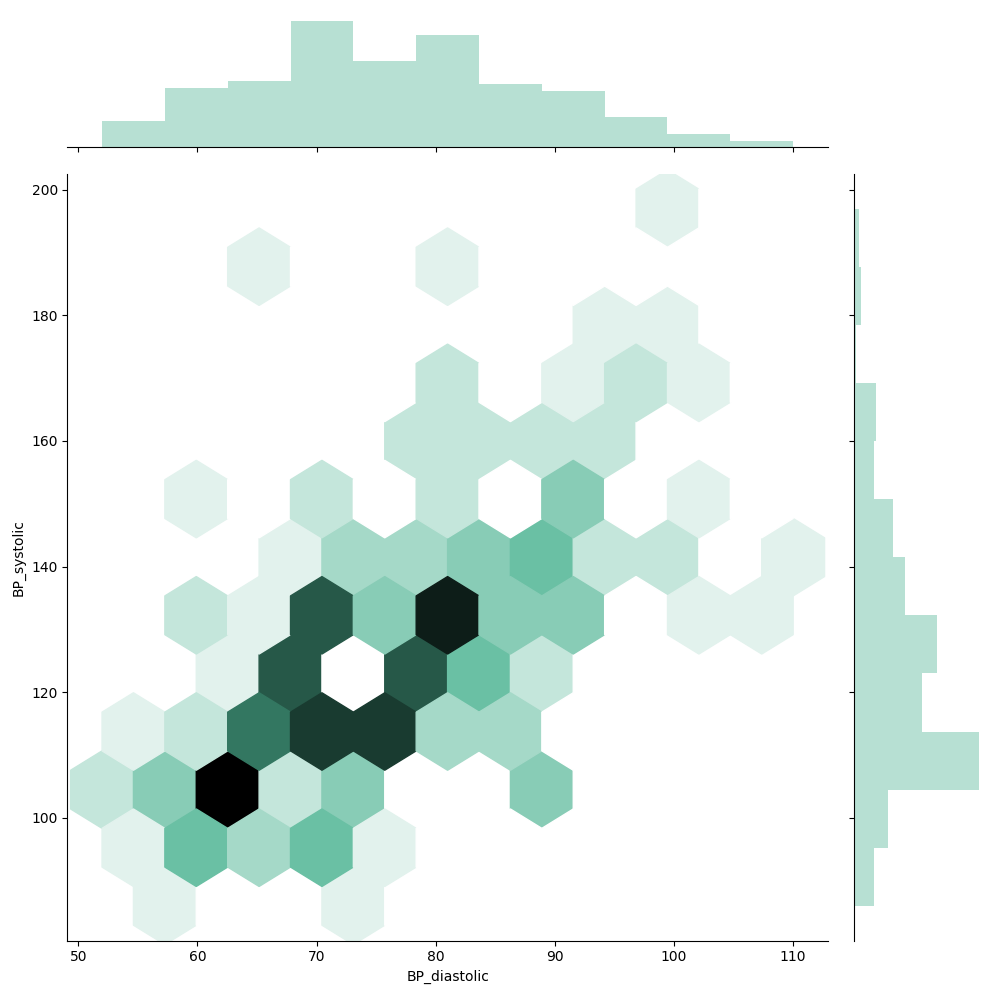
\includegraphics[width=0.4\textwidth]{data-exp/bp.png}
    %% Creator: Matplotlib, PGF backend
%%
%% To include the figure in your LaTeX document, write
%%   \input{<filename>.pgf}
%%
%% Make sure the required packages are loaded in your preamble
%%   \usepackage{pgf}
%%
%% Figures using additional raster images can only be included by \input if
%% they are in the same directory as the main LaTeX file. For loading figures
%% from other directories you can use the `import` package
%%   \usepackage{import}
%% and then include the figures with
%%   \import{<path to file>}{<filename>.pgf}
%%
%% Matplotlib used the following preamble
%%
\begingroup%
\makeatletter%
\begin{pgfpicture}%
\pgfpathrectangle{\pgfpointorigin}{\pgfqpoint{5.817937in}{2.961869in}}%
\pgfusepath{use as bounding box, clip}%
\begin{pgfscope}%
\pgfsetbuttcap%
\pgfsetmiterjoin%
\definecolor{currentfill}{rgb}{1.000000,1.000000,1.000000}%
\pgfsetfillcolor{currentfill}%
\pgfsetlinewidth{0.000000pt}%
\definecolor{currentstroke}{rgb}{1.000000,1.000000,1.000000}%
\pgfsetstrokecolor{currentstroke}%
\pgfsetdash{}{0pt}%
\pgfpathmoveto{\pgfqpoint{0.000000in}{0.000000in}}%
\pgfpathlineto{\pgfqpoint{5.817937in}{0.000000in}}%
\pgfpathlineto{\pgfqpoint{5.817937in}{2.961869in}}%
\pgfpathlineto{\pgfqpoint{0.000000in}{2.961869in}}%
\pgfpathclose%
\pgfusepath{fill}%
\end{pgfscope}%
\begin{pgfscope}%
\pgfsetbuttcap%
\pgfsetmiterjoin%
\definecolor{currentfill}{rgb}{0.917647,0.917647,0.949020}%
\pgfsetfillcolor{currentfill}%
\pgfsetlinewidth{0.000000pt}%
\definecolor{currentstroke}{rgb}{0.000000,0.000000,0.000000}%
\pgfsetstrokecolor{currentstroke}%
\pgfsetstrokeopacity{0.000000}%
\pgfsetdash{}{0pt}%
\pgfpathmoveto{\pgfqpoint{0.680437in}{0.583795in}}%
\pgfpathlineto{\pgfqpoint{5.717937in}{0.583795in}}%
\pgfpathlineto{\pgfqpoint{5.717937in}{2.662795in}}%
\pgfpathlineto{\pgfqpoint{0.680437in}{2.662795in}}%
\pgfpathclose%
\pgfusepath{fill}%
\end{pgfscope}%
\begin{pgfscope}%
\pgfpathrectangle{\pgfqpoint{0.680437in}{0.583795in}}{\pgfqpoint{5.037500in}{2.079000in}}%
\pgfusepath{clip}%
\pgfsetroundcap%
\pgfsetroundjoin%
\pgfsetlinewidth{1.003750pt}%
\definecolor{currentstroke}{rgb}{1.000000,1.000000,1.000000}%
\pgfsetstrokecolor{currentstroke}%
\pgfsetdash{}{0pt}%
\pgfpathmoveto{\pgfqpoint{0.752001in}{0.583795in}}%
\pgfpathlineto{\pgfqpoint{0.752001in}{2.662795in}}%
\pgfusepath{stroke}%
\end{pgfscope}%
\begin{pgfscope}%
\definecolor{textcolor}{rgb}{0.150000,0.150000,0.150000}%
\pgfsetstrokecolor{textcolor}%
\pgfsetfillcolor{textcolor}%
\pgftext[x=0.752001in,y=0.451851in,,top]{\color{textcolor}\sffamily\fontsize{12.000000}{14.400000}\selectfont \(\displaystyle 50\)}%
\end{pgfscope}%
\begin{pgfscope}%
\pgfpathrectangle{\pgfqpoint{0.680437in}{0.583795in}}{\pgfqpoint{5.037500in}{2.079000in}}%
\pgfusepath{clip}%
\pgfsetroundcap%
\pgfsetroundjoin%
\pgfsetlinewidth{1.003750pt}%
\definecolor{currentstroke}{rgb}{1.000000,1.000000,1.000000}%
\pgfsetstrokecolor{currentstroke}%
\pgfsetdash{}{0pt}%
\pgfpathmoveto{\pgfqpoint{1.541416in}{0.583795in}}%
\pgfpathlineto{\pgfqpoint{1.541416in}{2.662795in}}%
\pgfusepath{stroke}%
\end{pgfscope}%
\begin{pgfscope}%
\definecolor{textcolor}{rgb}{0.150000,0.150000,0.150000}%
\pgfsetstrokecolor{textcolor}%
\pgfsetfillcolor{textcolor}%
\pgftext[x=1.541416in,y=0.451851in,,top]{\color{textcolor}\sffamily\fontsize{12.000000}{14.400000}\selectfont \(\displaystyle 60\)}%
\end{pgfscope}%
\begin{pgfscope}%
\pgfpathrectangle{\pgfqpoint{0.680437in}{0.583795in}}{\pgfqpoint{5.037500in}{2.079000in}}%
\pgfusepath{clip}%
\pgfsetroundcap%
\pgfsetroundjoin%
\pgfsetlinewidth{1.003750pt}%
\definecolor{currentstroke}{rgb}{1.000000,1.000000,1.000000}%
\pgfsetstrokecolor{currentstroke}%
\pgfsetdash{}{0pt}%
\pgfpathmoveto{\pgfqpoint{2.330831in}{0.583795in}}%
\pgfpathlineto{\pgfqpoint{2.330831in}{2.662795in}}%
\pgfusepath{stroke}%
\end{pgfscope}%
\begin{pgfscope}%
\definecolor{textcolor}{rgb}{0.150000,0.150000,0.150000}%
\pgfsetstrokecolor{textcolor}%
\pgfsetfillcolor{textcolor}%
\pgftext[x=2.330831in,y=0.451851in,,top]{\color{textcolor}\sffamily\fontsize{12.000000}{14.400000}\selectfont \(\displaystyle 70\)}%
\end{pgfscope}%
\begin{pgfscope}%
\pgfpathrectangle{\pgfqpoint{0.680437in}{0.583795in}}{\pgfqpoint{5.037500in}{2.079000in}}%
\pgfusepath{clip}%
\pgfsetroundcap%
\pgfsetroundjoin%
\pgfsetlinewidth{1.003750pt}%
\definecolor{currentstroke}{rgb}{1.000000,1.000000,1.000000}%
\pgfsetstrokecolor{currentstroke}%
\pgfsetdash{}{0pt}%
\pgfpathmoveto{\pgfqpoint{3.120245in}{0.583795in}}%
\pgfpathlineto{\pgfqpoint{3.120245in}{2.662795in}}%
\pgfusepath{stroke}%
\end{pgfscope}%
\begin{pgfscope}%
\definecolor{textcolor}{rgb}{0.150000,0.150000,0.150000}%
\pgfsetstrokecolor{textcolor}%
\pgfsetfillcolor{textcolor}%
\pgftext[x=3.120245in,y=0.451851in,,top]{\color{textcolor}\sffamily\fontsize{12.000000}{14.400000}\selectfont \(\displaystyle 80\)}%
\end{pgfscope}%
\begin{pgfscope}%
\pgfpathrectangle{\pgfqpoint{0.680437in}{0.583795in}}{\pgfqpoint{5.037500in}{2.079000in}}%
\pgfusepath{clip}%
\pgfsetroundcap%
\pgfsetroundjoin%
\pgfsetlinewidth{1.003750pt}%
\definecolor{currentstroke}{rgb}{1.000000,1.000000,1.000000}%
\pgfsetstrokecolor{currentstroke}%
\pgfsetdash{}{0pt}%
\pgfpathmoveto{\pgfqpoint{3.909660in}{0.583795in}}%
\pgfpathlineto{\pgfqpoint{3.909660in}{2.662795in}}%
\pgfusepath{stroke}%
\end{pgfscope}%
\begin{pgfscope}%
\definecolor{textcolor}{rgb}{0.150000,0.150000,0.150000}%
\pgfsetstrokecolor{textcolor}%
\pgfsetfillcolor{textcolor}%
\pgftext[x=3.909660in,y=0.451851in,,top]{\color{textcolor}\sffamily\fontsize{12.000000}{14.400000}\selectfont \(\displaystyle 90\)}%
\end{pgfscope}%
\begin{pgfscope}%
\pgfpathrectangle{\pgfqpoint{0.680437in}{0.583795in}}{\pgfqpoint{5.037500in}{2.079000in}}%
\pgfusepath{clip}%
\pgfsetroundcap%
\pgfsetroundjoin%
\pgfsetlinewidth{1.003750pt}%
\definecolor{currentstroke}{rgb}{1.000000,1.000000,1.000000}%
\pgfsetstrokecolor{currentstroke}%
\pgfsetdash{}{0pt}%
\pgfpathmoveto{\pgfqpoint{4.699075in}{0.583795in}}%
\pgfpathlineto{\pgfqpoint{4.699075in}{2.662795in}}%
\pgfusepath{stroke}%
\end{pgfscope}%
\begin{pgfscope}%
\definecolor{textcolor}{rgb}{0.150000,0.150000,0.150000}%
\pgfsetstrokecolor{textcolor}%
\pgfsetfillcolor{textcolor}%
\pgftext[x=4.699075in,y=0.451851in,,top]{\color{textcolor}\sffamily\fontsize{12.000000}{14.400000}\selectfont \(\displaystyle 100\)}%
\end{pgfscope}%
\begin{pgfscope}%
\pgfpathrectangle{\pgfqpoint{0.680437in}{0.583795in}}{\pgfqpoint{5.037500in}{2.079000in}}%
\pgfusepath{clip}%
\pgfsetroundcap%
\pgfsetroundjoin%
\pgfsetlinewidth{1.003750pt}%
\definecolor{currentstroke}{rgb}{1.000000,1.000000,1.000000}%
\pgfsetstrokecolor{currentstroke}%
\pgfsetdash{}{0pt}%
\pgfpathmoveto{\pgfqpoint{5.488489in}{0.583795in}}%
\pgfpathlineto{\pgfqpoint{5.488489in}{2.662795in}}%
\pgfusepath{stroke}%
\end{pgfscope}%
\begin{pgfscope}%
\definecolor{textcolor}{rgb}{0.150000,0.150000,0.150000}%
\pgfsetstrokecolor{textcolor}%
\pgfsetfillcolor{textcolor}%
\pgftext[x=5.488489in,y=0.451851in,,top]{\color{textcolor}\sffamily\fontsize{12.000000}{14.400000}\selectfont \(\displaystyle 110\)}%
\end{pgfscope}%
\begin{pgfscope}%
\definecolor{textcolor}{rgb}{0.150000,0.150000,0.150000}%
\pgfsetstrokecolor{textcolor}%
\pgfsetfillcolor{textcolor}%
\pgftext[x=3.199187in,y=0.248148in,,top]{\color{textcolor}\sffamily\fontsize{12.000000}{14.400000}\selectfont Diastole}%
\end{pgfscope}%
\begin{pgfscope}%
\pgfpathrectangle{\pgfqpoint{0.680437in}{0.583795in}}{\pgfqpoint{5.037500in}{2.079000in}}%
\pgfusepath{clip}%
\pgfsetroundcap%
\pgfsetroundjoin%
\pgfsetlinewidth{1.003750pt}%
\definecolor{currentstroke}{rgb}{1.000000,1.000000,1.000000}%
\pgfsetstrokecolor{currentstroke}%
\pgfsetdash{}{0pt}%
\pgfpathmoveto{\pgfqpoint{0.680437in}{0.916857in}}%
\pgfpathlineto{\pgfqpoint{5.717937in}{0.916857in}}%
\pgfusepath{stroke}%
\end{pgfscope}%
\begin{pgfscope}%
\definecolor{textcolor}{rgb}{0.150000,0.150000,0.150000}%
\pgfsetstrokecolor{textcolor}%
\pgfsetfillcolor{textcolor}%
\pgftext[x=0.303703in,y=0.858987in,left,base]{\color{textcolor}\sffamily\fontsize{12.000000}{14.400000}\selectfont \(\displaystyle 100\)}%
\end{pgfscope}%
\begin{pgfscope}%
\pgfpathrectangle{\pgfqpoint{0.680437in}{0.583795in}}{\pgfqpoint{5.037500in}{2.079000in}}%
\pgfusepath{clip}%
\pgfsetroundcap%
\pgfsetroundjoin%
\pgfsetlinewidth{1.003750pt}%
\definecolor{currentstroke}{rgb}{1.000000,1.000000,1.000000}%
\pgfsetstrokecolor{currentstroke}%
\pgfsetdash{}{0pt}%
\pgfpathmoveto{\pgfqpoint{0.680437in}{1.342422in}}%
\pgfpathlineto{\pgfqpoint{5.717937in}{1.342422in}}%
\pgfusepath{stroke}%
\end{pgfscope}%
\begin{pgfscope}%
\definecolor{textcolor}{rgb}{0.150000,0.150000,0.150000}%
\pgfsetstrokecolor{textcolor}%
\pgfsetfillcolor{textcolor}%
\pgftext[x=0.303703in,y=1.284552in,left,base]{\color{textcolor}\sffamily\fontsize{12.000000}{14.400000}\selectfont \(\displaystyle 125\)}%
\end{pgfscope}%
\begin{pgfscope}%
\pgfpathrectangle{\pgfqpoint{0.680437in}{0.583795in}}{\pgfqpoint{5.037500in}{2.079000in}}%
\pgfusepath{clip}%
\pgfsetroundcap%
\pgfsetroundjoin%
\pgfsetlinewidth{1.003750pt}%
\definecolor{currentstroke}{rgb}{1.000000,1.000000,1.000000}%
\pgfsetstrokecolor{currentstroke}%
\pgfsetdash{}{0pt}%
\pgfpathmoveto{\pgfqpoint{0.680437in}{1.767987in}}%
\pgfpathlineto{\pgfqpoint{5.717937in}{1.767987in}}%
\pgfusepath{stroke}%
\end{pgfscope}%
\begin{pgfscope}%
\definecolor{textcolor}{rgb}{0.150000,0.150000,0.150000}%
\pgfsetstrokecolor{textcolor}%
\pgfsetfillcolor{textcolor}%
\pgftext[x=0.303703in,y=1.710117in,left,base]{\color{textcolor}\sffamily\fontsize{12.000000}{14.400000}\selectfont \(\displaystyle 150\)}%
\end{pgfscope}%
\begin{pgfscope}%
\pgfpathrectangle{\pgfqpoint{0.680437in}{0.583795in}}{\pgfqpoint{5.037500in}{2.079000in}}%
\pgfusepath{clip}%
\pgfsetroundcap%
\pgfsetroundjoin%
\pgfsetlinewidth{1.003750pt}%
\definecolor{currentstroke}{rgb}{1.000000,1.000000,1.000000}%
\pgfsetstrokecolor{currentstroke}%
\pgfsetdash{}{0pt}%
\pgfpathmoveto{\pgfqpoint{0.680437in}{2.193552in}}%
\pgfpathlineto{\pgfqpoint{5.717937in}{2.193552in}}%
\pgfusepath{stroke}%
\end{pgfscope}%
\begin{pgfscope}%
\definecolor{textcolor}{rgb}{0.150000,0.150000,0.150000}%
\pgfsetstrokecolor{textcolor}%
\pgfsetfillcolor{textcolor}%
\pgftext[x=0.303703in,y=2.135682in,left,base]{\color{textcolor}\sffamily\fontsize{12.000000}{14.400000}\selectfont \(\displaystyle 175\)}%
\end{pgfscope}%
\begin{pgfscope}%
\pgfpathrectangle{\pgfqpoint{0.680437in}{0.583795in}}{\pgfqpoint{5.037500in}{2.079000in}}%
\pgfusepath{clip}%
\pgfsetroundcap%
\pgfsetroundjoin%
\pgfsetlinewidth{1.003750pt}%
\definecolor{currentstroke}{rgb}{1.000000,1.000000,1.000000}%
\pgfsetstrokecolor{currentstroke}%
\pgfsetdash{}{0pt}%
\pgfpathmoveto{\pgfqpoint{0.680437in}{2.619117in}}%
\pgfpathlineto{\pgfqpoint{5.717937in}{2.619117in}}%
\pgfusepath{stroke}%
\end{pgfscope}%
\begin{pgfscope}%
\definecolor{textcolor}{rgb}{0.150000,0.150000,0.150000}%
\pgfsetstrokecolor{textcolor}%
\pgfsetfillcolor{textcolor}%
\pgftext[x=0.303703in,y=2.561247in,left,base]{\color{textcolor}\sffamily\fontsize{12.000000}{14.400000}\selectfont \(\displaystyle 200\)}%
\end{pgfscope}%
\begin{pgfscope}%
\definecolor{textcolor}{rgb}{0.150000,0.150000,0.150000}%
\pgfsetstrokecolor{textcolor}%
\pgfsetfillcolor{textcolor}%
\pgftext[x=0.248148in,y=1.623295in,,bottom,rotate=90.000000]{\color{textcolor}\sffamily\fontsize{12.000000}{14.400000}\selectfont Systole}%
\end{pgfscope}%
\begin{pgfscope}%
\pgfpathrectangle{\pgfqpoint{0.680437in}{0.583795in}}{\pgfqpoint{5.037500in}{2.079000in}}%
\pgfusepath{clip}%
\pgfsetbuttcap%
\pgfsetroundjoin%
\definecolor{currentfill}{rgb}{0.298039,0.447059,0.690196}%
\pgfsetfillcolor{currentfill}%
\pgfsetlinewidth{1.003750pt}%
\definecolor{currentstroke}{rgb}{0.298039,0.447059,0.690196}%
\pgfsetstrokecolor{currentstroke}%
\pgfsetdash{}{0pt}%
\pgfpathmoveto{\pgfqpoint{2.330831in}{1.215642in}}%
\pgfpathcurveto{\pgfqpoint{2.341881in}{1.215642in}}{\pgfqpoint{2.352480in}{1.220033in}}{\pgfqpoint{2.360293in}{1.227846in}}%
\pgfpathcurveto{\pgfqpoint{2.368107in}{1.235660in}}{\pgfqpoint{2.372497in}{1.246259in}}{\pgfqpoint{2.372497in}{1.257309in}}%
\pgfpathcurveto{\pgfqpoint{2.372497in}{1.268359in}}{\pgfqpoint{2.368107in}{1.278958in}}{\pgfqpoint{2.360293in}{1.286772in}}%
\pgfpathcurveto{\pgfqpoint{2.352480in}{1.294585in}}{\pgfqpoint{2.341881in}{1.298976in}}{\pgfqpoint{2.330831in}{1.298976in}}%
\pgfpathcurveto{\pgfqpoint{2.319780in}{1.298976in}}{\pgfqpoint{2.309181in}{1.294585in}}{\pgfqpoint{2.301368in}{1.286772in}}%
\pgfpathcurveto{\pgfqpoint{2.293554in}{1.278958in}}{\pgfqpoint{2.289164in}{1.268359in}}{\pgfqpoint{2.289164in}{1.257309in}}%
\pgfpathcurveto{\pgfqpoint{2.289164in}{1.246259in}}{\pgfqpoint{2.293554in}{1.235660in}}{\pgfqpoint{2.301368in}{1.227846in}}%
\pgfpathcurveto{\pgfqpoint{2.309181in}{1.220033in}}{\pgfqpoint{2.319780in}{1.215642in}}{\pgfqpoint{2.330831in}{1.215642in}}%
\pgfpathclose%
\pgfusepath{stroke,fill}%
\end{pgfscope}%
\begin{pgfscope}%
\pgfpathrectangle{\pgfqpoint{0.680437in}{0.583795in}}{\pgfqpoint{5.037500in}{2.079000in}}%
\pgfusepath{clip}%
\pgfsetbuttcap%
\pgfsetroundjoin%
\definecolor{currentfill}{rgb}{0.298039,0.447059,0.690196}%
\pgfsetfillcolor{currentfill}%
\pgfsetlinewidth{1.003750pt}%
\definecolor{currentstroke}{rgb}{0.298039,0.447059,0.690196}%
\pgfsetstrokecolor{currentstroke}%
\pgfsetdash{}{0pt}%
\pgfpathmoveto{\pgfqpoint{3.120245in}{1.385868in}}%
\pgfpathcurveto{\pgfqpoint{3.131295in}{1.385868in}}{\pgfqpoint{3.141894in}{1.390259in}}{\pgfqpoint{3.149708in}{1.398072in}}%
\pgfpathcurveto{\pgfqpoint{3.157522in}{1.405886in}}{\pgfqpoint{3.161912in}{1.416485in}}{\pgfqpoint{3.161912in}{1.427535in}}%
\pgfpathcurveto{\pgfqpoint{3.161912in}{1.438585in}}{\pgfqpoint{3.157522in}{1.449184in}}{\pgfqpoint{3.149708in}{1.456998in}}%
\pgfpathcurveto{\pgfqpoint{3.141894in}{1.464811in}}{\pgfqpoint{3.131295in}{1.469202in}}{\pgfqpoint{3.120245in}{1.469202in}}%
\pgfpathcurveto{\pgfqpoint{3.109195in}{1.469202in}}{\pgfqpoint{3.098596in}{1.464811in}}{\pgfqpoint{3.090782in}{1.456998in}}%
\pgfpathcurveto{\pgfqpoint{3.082969in}{1.449184in}}{\pgfqpoint{3.078579in}{1.438585in}}{\pgfqpoint{3.078579in}{1.427535in}}%
\pgfpathcurveto{\pgfqpoint{3.078579in}{1.416485in}}{\pgfqpoint{3.082969in}{1.405886in}}{\pgfqpoint{3.090782in}{1.398072in}}%
\pgfpathcurveto{\pgfqpoint{3.098596in}{1.390259in}}{\pgfqpoint{3.109195in}{1.385868in}}{\pgfqpoint{3.120245in}{1.385868in}}%
\pgfpathclose%
\pgfusepath{stroke,fill}%
\end{pgfscope}%
\begin{pgfscope}%
\pgfpathrectangle{\pgfqpoint{0.680437in}{0.583795in}}{\pgfqpoint{5.037500in}{2.079000in}}%
\pgfusepath{clip}%
\pgfsetbuttcap%
\pgfsetroundjoin%
\definecolor{currentfill}{rgb}{0.298039,0.447059,0.690196}%
\pgfsetfillcolor{currentfill}%
\pgfsetlinewidth{1.003750pt}%
\definecolor{currentstroke}{rgb}{0.298039,0.447059,0.690196}%
\pgfsetstrokecolor{currentstroke}%
\pgfsetdash{}{0pt}%
\pgfpathmoveto{\pgfqpoint{3.909660in}{0.960303in}}%
\pgfpathcurveto{\pgfqpoint{3.920710in}{0.960303in}}{\pgfqpoint{3.931309in}{0.964694in}}{\pgfqpoint{3.939123in}{0.972507in}}%
\pgfpathcurveto{\pgfqpoint{3.946936in}{0.980321in}}{\pgfqpoint{3.951327in}{0.990920in}}{\pgfqpoint{3.951327in}{1.001970in}}%
\pgfpathcurveto{\pgfqpoint{3.951327in}{1.013020in}}{\pgfqpoint{3.946936in}{1.023619in}}{\pgfqpoint{3.939123in}{1.031433in}}%
\pgfpathcurveto{\pgfqpoint{3.931309in}{1.039246in}}{\pgfqpoint{3.920710in}{1.043637in}}{\pgfqpoint{3.909660in}{1.043637in}}%
\pgfpathcurveto{\pgfqpoint{3.898610in}{1.043637in}}{\pgfqpoint{3.888011in}{1.039246in}}{\pgfqpoint{3.880197in}{1.031433in}}%
\pgfpathcurveto{\pgfqpoint{3.872383in}{1.023619in}}{\pgfqpoint{3.867993in}{1.013020in}}{\pgfqpoint{3.867993in}{1.001970in}}%
\pgfpathcurveto{\pgfqpoint{3.867993in}{0.990920in}}{\pgfqpoint{3.872383in}{0.980321in}}{\pgfqpoint{3.880197in}{0.972507in}}%
\pgfpathcurveto{\pgfqpoint{3.888011in}{0.964694in}}{\pgfqpoint{3.898610in}{0.960303in}}{\pgfqpoint{3.909660in}{0.960303in}}%
\pgfpathclose%
\pgfusepath{stroke,fill}%
\end{pgfscope}%
\begin{pgfscope}%
\pgfpathrectangle{\pgfqpoint{0.680437in}{0.583795in}}{\pgfqpoint{5.037500in}{2.079000in}}%
\pgfusepath{clip}%
\pgfsetbuttcap%
\pgfsetroundjoin%
\definecolor{currentfill}{rgb}{0.298039,0.447059,0.690196}%
\pgfsetfillcolor{currentfill}%
\pgfsetlinewidth{1.003750pt}%
\definecolor{currentstroke}{rgb}{0.298039,0.447059,0.690196}%
\pgfsetstrokecolor{currentstroke}%
\pgfsetdash{}{0pt}%
\pgfpathmoveto{\pgfqpoint{1.936123in}{0.960303in}}%
\pgfpathcurveto{\pgfqpoint{1.947173in}{0.960303in}}{\pgfqpoint{1.957772in}{0.964694in}}{\pgfqpoint{1.965586in}{0.972507in}}%
\pgfpathcurveto{\pgfqpoint{1.973400in}{0.980321in}}{\pgfqpoint{1.977790in}{0.990920in}}{\pgfqpoint{1.977790in}{1.001970in}}%
\pgfpathcurveto{\pgfqpoint{1.977790in}{1.013020in}}{\pgfqpoint{1.973400in}{1.023619in}}{\pgfqpoint{1.965586in}{1.031433in}}%
\pgfpathcurveto{\pgfqpoint{1.957772in}{1.039246in}}{\pgfqpoint{1.947173in}{1.043637in}}{\pgfqpoint{1.936123in}{1.043637in}}%
\pgfpathcurveto{\pgfqpoint{1.925073in}{1.043637in}}{\pgfqpoint{1.914474in}{1.039246in}}{\pgfqpoint{1.906660in}{1.031433in}}%
\pgfpathcurveto{\pgfqpoint{1.898847in}{1.023619in}}{\pgfqpoint{1.894456in}{1.013020in}}{\pgfqpoint{1.894456in}{1.001970in}}%
\pgfpathcurveto{\pgfqpoint{1.894456in}{0.990920in}}{\pgfqpoint{1.898847in}{0.980321in}}{\pgfqpoint{1.906660in}{0.972507in}}%
\pgfpathcurveto{\pgfqpoint{1.914474in}{0.964694in}}{\pgfqpoint{1.925073in}{0.960303in}}{\pgfqpoint{1.936123in}{0.960303in}}%
\pgfpathclose%
\pgfusepath{stroke,fill}%
\end{pgfscope}%
\begin{pgfscope}%
\pgfpathrectangle{\pgfqpoint{0.680437in}{0.583795in}}{\pgfqpoint{5.037500in}{2.079000in}}%
\pgfusepath{clip}%
\pgfsetbuttcap%
\pgfsetroundjoin%
\definecolor{currentfill}{rgb}{0.298039,0.447059,0.690196}%
\pgfsetfillcolor{currentfill}%
\pgfsetlinewidth{1.003750pt}%
\definecolor{currentstroke}{rgb}{0.298039,0.447059,0.690196}%
\pgfsetstrokecolor{currentstroke}%
\pgfsetdash{}{0pt}%
\pgfpathmoveto{\pgfqpoint{1.936123in}{1.045416in}}%
\pgfpathcurveto{\pgfqpoint{1.947173in}{1.045416in}}{\pgfqpoint{1.957772in}{1.049807in}}{\pgfqpoint{1.965586in}{1.057620in}}%
\pgfpathcurveto{\pgfqpoint{1.973400in}{1.065434in}}{\pgfqpoint{1.977790in}{1.076033in}}{\pgfqpoint{1.977790in}{1.087083in}}%
\pgfpathcurveto{\pgfqpoint{1.977790in}{1.098133in}}{\pgfqpoint{1.973400in}{1.108732in}}{\pgfqpoint{1.965586in}{1.116546in}}%
\pgfpathcurveto{\pgfqpoint{1.957772in}{1.124359in}}{\pgfqpoint{1.947173in}{1.128750in}}{\pgfqpoint{1.936123in}{1.128750in}}%
\pgfpathcurveto{\pgfqpoint{1.925073in}{1.128750in}}{\pgfqpoint{1.914474in}{1.124359in}}{\pgfqpoint{1.906660in}{1.116546in}}%
\pgfpathcurveto{\pgfqpoint{1.898847in}{1.108732in}}{\pgfqpoint{1.894456in}{1.098133in}}{\pgfqpoint{1.894456in}{1.087083in}}%
\pgfpathcurveto{\pgfqpoint{1.894456in}{1.076033in}}{\pgfqpoint{1.898847in}{1.065434in}}{\pgfqpoint{1.906660in}{1.057620in}}%
\pgfpathcurveto{\pgfqpoint{1.914474in}{1.049807in}}{\pgfqpoint{1.925073in}{1.045416in}}{\pgfqpoint{1.936123in}{1.045416in}}%
\pgfpathclose%
\pgfusepath{stroke,fill}%
\end{pgfscope}%
\begin{pgfscope}%
\pgfpathrectangle{\pgfqpoint{0.680437in}{0.583795in}}{\pgfqpoint{5.037500in}{2.079000in}}%
\pgfusepath{clip}%
\pgfsetbuttcap%
\pgfsetroundjoin%
\definecolor{currentfill}{rgb}{0.298039,0.447059,0.690196}%
\pgfsetfillcolor{currentfill}%
\pgfsetlinewidth{1.003750pt}%
\definecolor{currentstroke}{rgb}{0.298039,0.447059,0.690196}%
\pgfsetstrokecolor{currentstroke}%
\pgfsetdash{}{0pt}%
\pgfpathmoveto{\pgfqpoint{2.330831in}{1.215642in}}%
\pgfpathcurveto{\pgfqpoint{2.341881in}{1.215642in}}{\pgfqpoint{2.352480in}{1.220033in}}{\pgfqpoint{2.360293in}{1.227846in}}%
\pgfpathcurveto{\pgfqpoint{2.368107in}{1.235660in}}{\pgfqpoint{2.372497in}{1.246259in}}{\pgfqpoint{2.372497in}{1.257309in}}%
\pgfpathcurveto{\pgfqpoint{2.372497in}{1.268359in}}{\pgfqpoint{2.368107in}{1.278958in}}{\pgfqpoint{2.360293in}{1.286772in}}%
\pgfpathcurveto{\pgfqpoint{2.352480in}{1.294585in}}{\pgfqpoint{2.341881in}{1.298976in}}{\pgfqpoint{2.330831in}{1.298976in}}%
\pgfpathcurveto{\pgfqpoint{2.319780in}{1.298976in}}{\pgfqpoint{2.309181in}{1.294585in}}{\pgfqpoint{2.301368in}{1.286772in}}%
\pgfpathcurveto{\pgfqpoint{2.293554in}{1.278958in}}{\pgfqpoint{2.289164in}{1.268359in}}{\pgfqpoint{2.289164in}{1.257309in}}%
\pgfpathcurveto{\pgfqpoint{2.289164in}{1.246259in}}{\pgfqpoint{2.293554in}{1.235660in}}{\pgfqpoint{2.301368in}{1.227846in}}%
\pgfpathcurveto{\pgfqpoint{2.309181in}{1.220033in}}{\pgfqpoint{2.319780in}{1.215642in}}{\pgfqpoint{2.330831in}{1.215642in}}%
\pgfpathclose%
\pgfusepath{stroke,fill}%
\end{pgfscope}%
\begin{pgfscope}%
\pgfpathrectangle{\pgfqpoint{0.680437in}{0.583795in}}{\pgfqpoint{5.037500in}{2.079000in}}%
\pgfusepath{clip}%
\pgfsetbuttcap%
\pgfsetroundjoin%
\definecolor{currentfill}{rgb}{0.298039,0.447059,0.690196}%
\pgfsetfillcolor{currentfill}%
\pgfsetlinewidth{1.003750pt}%
\definecolor{currentstroke}{rgb}{0.298039,0.447059,0.690196}%
\pgfsetstrokecolor{currentstroke}%
\pgfsetdash{}{0pt}%
\pgfpathmoveto{\pgfqpoint{3.120245in}{1.385868in}}%
\pgfpathcurveto{\pgfqpoint{3.131295in}{1.385868in}}{\pgfqpoint{3.141894in}{1.390259in}}{\pgfqpoint{3.149708in}{1.398072in}}%
\pgfpathcurveto{\pgfqpoint{3.157522in}{1.405886in}}{\pgfqpoint{3.161912in}{1.416485in}}{\pgfqpoint{3.161912in}{1.427535in}}%
\pgfpathcurveto{\pgfqpoint{3.161912in}{1.438585in}}{\pgfqpoint{3.157522in}{1.449184in}}{\pgfqpoint{3.149708in}{1.456998in}}%
\pgfpathcurveto{\pgfqpoint{3.141894in}{1.464811in}}{\pgfqpoint{3.131295in}{1.469202in}}{\pgfqpoint{3.120245in}{1.469202in}}%
\pgfpathcurveto{\pgfqpoint{3.109195in}{1.469202in}}{\pgfqpoint{3.098596in}{1.464811in}}{\pgfqpoint{3.090782in}{1.456998in}}%
\pgfpathcurveto{\pgfqpoint{3.082969in}{1.449184in}}{\pgfqpoint{3.078579in}{1.438585in}}{\pgfqpoint{3.078579in}{1.427535in}}%
\pgfpathcurveto{\pgfqpoint{3.078579in}{1.416485in}}{\pgfqpoint{3.082969in}{1.405886in}}{\pgfqpoint{3.090782in}{1.398072in}}%
\pgfpathcurveto{\pgfqpoint{3.098596in}{1.390259in}}{\pgfqpoint{3.109195in}{1.385868in}}{\pgfqpoint{3.120245in}{1.385868in}}%
\pgfpathclose%
\pgfusepath{stroke,fill}%
\end{pgfscope}%
\begin{pgfscope}%
\pgfpathrectangle{\pgfqpoint{0.680437in}{0.583795in}}{\pgfqpoint{5.037500in}{2.079000in}}%
\pgfusepath{clip}%
\pgfsetbuttcap%
\pgfsetroundjoin%
\definecolor{currentfill}{rgb}{0.298039,0.447059,0.690196}%
\pgfsetfillcolor{currentfill}%
\pgfsetlinewidth{1.003750pt}%
\definecolor{currentstroke}{rgb}{0.298039,0.447059,0.690196}%
\pgfsetstrokecolor{currentstroke}%
\pgfsetdash{}{0pt}%
\pgfpathmoveto{\pgfqpoint{3.120245in}{1.385868in}}%
\pgfpathcurveto{\pgfqpoint{3.131295in}{1.385868in}}{\pgfqpoint{3.141894in}{1.390259in}}{\pgfqpoint{3.149708in}{1.398072in}}%
\pgfpathcurveto{\pgfqpoint{3.157522in}{1.405886in}}{\pgfqpoint{3.161912in}{1.416485in}}{\pgfqpoint{3.161912in}{1.427535in}}%
\pgfpathcurveto{\pgfqpoint{3.161912in}{1.438585in}}{\pgfqpoint{3.157522in}{1.449184in}}{\pgfqpoint{3.149708in}{1.456998in}}%
\pgfpathcurveto{\pgfqpoint{3.141894in}{1.464811in}}{\pgfqpoint{3.131295in}{1.469202in}}{\pgfqpoint{3.120245in}{1.469202in}}%
\pgfpathcurveto{\pgfqpoint{3.109195in}{1.469202in}}{\pgfqpoint{3.098596in}{1.464811in}}{\pgfqpoint{3.090782in}{1.456998in}}%
\pgfpathcurveto{\pgfqpoint{3.082969in}{1.449184in}}{\pgfqpoint{3.078579in}{1.438585in}}{\pgfqpoint{3.078579in}{1.427535in}}%
\pgfpathcurveto{\pgfqpoint{3.078579in}{1.416485in}}{\pgfqpoint{3.082969in}{1.405886in}}{\pgfqpoint{3.090782in}{1.398072in}}%
\pgfpathcurveto{\pgfqpoint{3.098596in}{1.390259in}}{\pgfqpoint{3.109195in}{1.385868in}}{\pgfqpoint{3.120245in}{1.385868in}}%
\pgfpathclose%
\pgfusepath{stroke,fill}%
\end{pgfscope}%
\begin{pgfscope}%
\pgfpathrectangle{\pgfqpoint{0.680437in}{0.583795in}}{\pgfqpoint{5.037500in}{2.079000in}}%
\pgfusepath{clip}%
\pgfsetbuttcap%
\pgfsetroundjoin%
\definecolor{currentfill}{rgb}{0.298039,0.447059,0.690196}%
\pgfsetfillcolor{currentfill}%
\pgfsetlinewidth{1.003750pt}%
\definecolor{currentstroke}{rgb}{0.298039,0.447059,0.690196}%
\pgfsetstrokecolor{currentstroke}%
\pgfsetdash{}{0pt}%
\pgfpathmoveto{\pgfqpoint{1.936123in}{1.130529in}}%
\pgfpathcurveto{\pgfqpoint{1.947173in}{1.130529in}}{\pgfqpoint{1.957772in}{1.134920in}}{\pgfqpoint{1.965586in}{1.142733in}}%
\pgfpathcurveto{\pgfqpoint{1.973400in}{1.150547in}}{\pgfqpoint{1.977790in}{1.161146in}}{\pgfqpoint{1.977790in}{1.172196in}}%
\pgfpathcurveto{\pgfqpoint{1.977790in}{1.183246in}}{\pgfqpoint{1.973400in}{1.193845in}}{\pgfqpoint{1.965586in}{1.201659in}}%
\pgfpathcurveto{\pgfqpoint{1.957772in}{1.209472in}}{\pgfqpoint{1.947173in}{1.213863in}}{\pgfqpoint{1.936123in}{1.213863in}}%
\pgfpathcurveto{\pgfqpoint{1.925073in}{1.213863in}}{\pgfqpoint{1.914474in}{1.209472in}}{\pgfqpoint{1.906660in}{1.201659in}}%
\pgfpathcurveto{\pgfqpoint{1.898847in}{1.193845in}}{\pgfqpoint{1.894456in}{1.183246in}}{\pgfqpoint{1.894456in}{1.172196in}}%
\pgfpathcurveto{\pgfqpoint{1.894456in}{1.161146in}}{\pgfqpoint{1.898847in}{1.150547in}}{\pgfqpoint{1.906660in}{1.142733in}}%
\pgfpathcurveto{\pgfqpoint{1.914474in}{1.134920in}}{\pgfqpoint{1.925073in}{1.130529in}}{\pgfqpoint{1.936123in}{1.130529in}}%
\pgfpathclose%
\pgfusepath{stroke,fill}%
\end{pgfscope}%
\begin{pgfscope}%
\pgfpathrectangle{\pgfqpoint{0.680437in}{0.583795in}}{\pgfqpoint{5.037500in}{2.079000in}}%
\pgfusepath{clip}%
\pgfsetbuttcap%
\pgfsetroundjoin%
\definecolor{currentfill}{rgb}{0.298039,0.447059,0.690196}%
\pgfsetfillcolor{currentfill}%
\pgfsetlinewidth{1.003750pt}%
\definecolor{currentstroke}{rgb}{0.298039,0.447059,0.690196}%
\pgfsetstrokecolor{currentstroke}%
\pgfsetdash{}{0pt}%
\pgfpathmoveto{\pgfqpoint{2.646596in}{1.011371in}}%
\pgfpathcurveto{\pgfqpoint{2.657647in}{1.011371in}}{\pgfqpoint{2.668246in}{1.015761in}}{\pgfqpoint{2.676059in}{1.023575in}}%
\pgfpathcurveto{\pgfqpoint{2.683873in}{1.031389in}}{\pgfqpoint{2.688263in}{1.041988in}}{\pgfqpoint{2.688263in}{1.053038in}}%
\pgfpathcurveto{\pgfqpoint{2.688263in}{1.064088in}}{\pgfqpoint{2.683873in}{1.074687in}}{\pgfqpoint{2.676059in}{1.082501in}}%
\pgfpathcurveto{\pgfqpoint{2.668246in}{1.090314in}}{\pgfqpoint{2.657647in}{1.094705in}}{\pgfqpoint{2.646596in}{1.094705in}}%
\pgfpathcurveto{\pgfqpoint{2.635546in}{1.094705in}}{\pgfqpoint{2.624947in}{1.090314in}}{\pgfqpoint{2.617134in}{1.082501in}}%
\pgfpathcurveto{\pgfqpoint{2.609320in}{1.074687in}}{\pgfqpoint{2.604930in}{1.064088in}}{\pgfqpoint{2.604930in}{1.053038in}}%
\pgfpathcurveto{\pgfqpoint{2.604930in}{1.041988in}}{\pgfqpoint{2.609320in}{1.031389in}}{\pgfqpoint{2.617134in}{1.023575in}}%
\pgfpathcurveto{\pgfqpoint{2.624947in}{1.015761in}}{\pgfqpoint{2.635546in}{1.011371in}}{\pgfqpoint{2.646596in}{1.011371in}}%
\pgfpathclose%
\pgfusepath{stroke,fill}%
\end{pgfscope}%
\begin{pgfscope}%
\pgfpathrectangle{\pgfqpoint{0.680437in}{0.583795in}}{\pgfqpoint{5.037500in}{2.079000in}}%
\pgfusepath{clip}%
\pgfsetbuttcap%
\pgfsetroundjoin%
\definecolor{currentfill}{rgb}{0.298039,0.447059,0.690196}%
\pgfsetfillcolor{currentfill}%
\pgfsetlinewidth{1.003750pt}%
\definecolor{currentstroke}{rgb}{0.298039,0.447059,0.690196}%
\pgfsetstrokecolor{currentstroke}%
\pgfsetdash{}{0pt}%
\pgfpathmoveto{\pgfqpoint{3.672835in}{1.011371in}}%
\pgfpathcurveto{\pgfqpoint{3.683886in}{1.011371in}}{\pgfqpoint{3.694485in}{1.015761in}}{\pgfqpoint{3.702298in}{1.023575in}}%
\pgfpathcurveto{\pgfqpoint{3.710112in}{1.031389in}}{\pgfqpoint{3.714502in}{1.041988in}}{\pgfqpoint{3.714502in}{1.053038in}}%
\pgfpathcurveto{\pgfqpoint{3.714502in}{1.064088in}}{\pgfqpoint{3.710112in}{1.074687in}}{\pgfqpoint{3.702298in}{1.082501in}}%
\pgfpathcurveto{\pgfqpoint{3.694485in}{1.090314in}}{\pgfqpoint{3.683886in}{1.094705in}}{\pgfqpoint{3.672835in}{1.094705in}}%
\pgfpathcurveto{\pgfqpoint{3.661785in}{1.094705in}}{\pgfqpoint{3.651186in}{1.090314in}}{\pgfqpoint{3.643373in}{1.082501in}}%
\pgfpathcurveto{\pgfqpoint{3.635559in}{1.074687in}}{\pgfqpoint{3.631169in}{1.064088in}}{\pgfqpoint{3.631169in}{1.053038in}}%
\pgfpathcurveto{\pgfqpoint{3.631169in}{1.041988in}}{\pgfqpoint{3.635559in}{1.031389in}}{\pgfqpoint{3.643373in}{1.023575in}}%
\pgfpathcurveto{\pgfqpoint{3.651186in}{1.015761in}}{\pgfqpoint{3.661785in}{1.011371in}}{\pgfqpoint{3.672835in}{1.011371in}}%
\pgfpathclose%
\pgfusepath{stroke,fill}%
\end{pgfscope}%
\begin{pgfscope}%
\pgfpathrectangle{\pgfqpoint{0.680437in}{0.583795in}}{\pgfqpoint{5.037500in}{2.079000in}}%
\pgfusepath{clip}%
\pgfsetbuttcap%
\pgfsetroundjoin%
\definecolor{currentfill}{rgb}{0.298039,0.447059,0.690196}%
\pgfsetfillcolor{currentfill}%
\pgfsetlinewidth{1.003750pt}%
\definecolor{currentstroke}{rgb}{0.298039,0.447059,0.690196}%
\pgfsetstrokecolor{currentstroke}%
\pgfsetdash{}{0pt}%
\pgfpathmoveto{\pgfqpoint{2.330831in}{1.045416in}}%
\pgfpathcurveto{\pgfqpoint{2.341881in}{1.045416in}}{\pgfqpoint{2.352480in}{1.049807in}}{\pgfqpoint{2.360293in}{1.057620in}}%
\pgfpathcurveto{\pgfqpoint{2.368107in}{1.065434in}}{\pgfqpoint{2.372497in}{1.076033in}}{\pgfqpoint{2.372497in}{1.087083in}}%
\pgfpathcurveto{\pgfqpoint{2.372497in}{1.098133in}}{\pgfqpoint{2.368107in}{1.108732in}}{\pgfqpoint{2.360293in}{1.116546in}}%
\pgfpathcurveto{\pgfqpoint{2.352480in}{1.124359in}}{\pgfqpoint{2.341881in}{1.128750in}}{\pgfqpoint{2.330831in}{1.128750in}}%
\pgfpathcurveto{\pgfqpoint{2.319780in}{1.128750in}}{\pgfqpoint{2.309181in}{1.124359in}}{\pgfqpoint{2.301368in}{1.116546in}}%
\pgfpathcurveto{\pgfqpoint{2.293554in}{1.108732in}}{\pgfqpoint{2.289164in}{1.098133in}}{\pgfqpoint{2.289164in}{1.087083in}}%
\pgfpathcurveto{\pgfqpoint{2.289164in}{1.076033in}}{\pgfqpoint{2.293554in}{1.065434in}}{\pgfqpoint{2.301368in}{1.057620in}}%
\pgfpathcurveto{\pgfqpoint{2.309181in}{1.049807in}}{\pgfqpoint{2.319780in}{1.045416in}}{\pgfqpoint{2.330831in}{1.045416in}}%
\pgfpathclose%
\pgfusepath{stroke,fill}%
\end{pgfscope}%
\begin{pgfscope}%
\pgfpathrectangle{\pgfqpoint{0.680437in}{0.583795in}}{\pgfqpoint{5.037500in}{2.079000in}}%
\pgfusepath{clip}%
\pgfsetbuttcap%
\pgfsetroundjoin%
\definecolor{currentfill}{rgb}{0.298039,0.447059,0.690196}%
\pgfsetfillcolor{currentfill}%
\pgfsetlinewidth{1.003750pt}%
\definecolor{currentstroke}{rgb}{0.298039,0.447059,0.690196}%
\pgfsetstrokecolor{currentstroke}%
\pgfsetdash{}{0pt}%
\pgfpathmoveto{\pgfqpoint{3.514953in}{1.215642in}}%
\pgfpathcurveto{\pgfqpoint{3.526003in}{1.215642in}}{\pgfqpoint{3.536602in}{1.220033in}}{\pgfqpoint{3.544415in}{1.227846in}}%
\pgfpathcurveto{\pgfqpoint{3.552229in}{1.235660in}}{\pgfqpoint{3.556619in}{1.246259in}}{\pgfqpoint{3.556619in}{1.257309in}}%
\pgfpathcurveto{\pgfqpoint{3.556619in}{1.268359in}}{\pgfqpoint{3.552229in}{1.278958in}}{\pgfqpoint{3.544415in}{1.286772in}}%
\pgfpathcurveto{\pgfqpoint{3.536602in}{1.294585in}}{\pgfqpoint{3.526003in}{1.298976in}}{\pgfqpoint{3.514953in}{1.298976in}}%
\pgfpathcurveto{\pgfqpoint{3.503902in}{1.298976in}}{\pgfqpoint{3.493303in}{1.294585in}}{\pgfqpoint{3.485490in}{1.286772in}}%
\pgfpathcurveto{\pgfqpoint{3.477676in}{1.278958in}}{\pgfqpoint{3.473286in}{1.268359in}}{\pgfqpoint{3.473286in}{1.257309in}}%
\pgfpathcurveto{\pgfqpoint{3.473286in}{1.246259in}}{\pgfqpoint{3.477676in}{1.235660in}}{\pgfqpoint{3.485490in}{1.227846in}}%
\pgfpathcurveto{\pgfqpoint{3.493303in}{1.220033in}}{\pgfqpoint{3.503902in}{1.215642in}}{\pgfqpoint{3.514953in}{1.215642in}}%
\pgfpathclose%
\pgfusepath{stroke,fill}%
\end{pgfscope}%
\begin{pgfscope}%
\pgfpathrectangle{\pgfqpoint{0.680437in}{0.583795in}}{\pgfqpoint{5.037500in}{2.079000in}}%
\pgfusepath{clip}%
\pgfsetbuttcap%
\pgfsetroundjoin%
\definecolor{currentfill}{rgb}{0.298039,0.447059,0.690196}%
\pgfsetfillcolor{currentfill}%
\pgfsetlinewidth{1.003750pt}%
\definecolor{currentstroke}{rgb}{0.298039,0.447059,0.690196}%
\pgfsetstrokecolor{currentstroke}%
\pgfsetdash{}{0pt}%
\pgfpathmoveto{\pgfqpoint{2.330831in}{1.045416in}}%
\pgfpathcurveto{\pgfqpoint{2.341881in}{1.045416in}}{\pgfqpoint{2.352480in}{1.049807in}}{\pgfqpoint{2.360293in}{1.057620in}}%
\pgfpathcurveto{\pgfqpoint{2.368107in}{1.065434in}}{\pgfqpoint{2.372497in}{1.076033in}}{\pgfqpoint{2.372497in}{1.087083in}}%
\pgfpathcurveto{\pgfqpoint{2.372497in}{1.098133in}}{\pgfqpoint{2.368107in}{1.108732in}}{\pgfqpoint{2.360293in}{1.116546in}}%
\pgfpathcurveto{\pgfqpoint{2.352480in}{1.124359in}}{\pgfqpoint{2.341881in}{1.128750in}}{\pgfqpoint{2.330831in}{1.128750in}}%
\pgfpathcurveto{\pgfqpoint{2.319780in}{1.128750in}}{\pgfqpoint{2.309181in}{1.124359in}}{\pgfqpoint{2.301368in}{1.116546in}}%
\pgfpathcurveto{\pgfqpoint{2.293554in}{1.108732in}}{\pgfqpoint{2.289164in}{1.098133in}}{\pgfqpoint{2.289164in}{1.087083in}}%
\pgfpathcurveto{\pgfqpoint{2.289164in}{1.076033in}}{\pgfqpoint{2.293554in}{1.065434in}}{\pgfqpoint{2.301368in}{1.057620in}}%
\pgfpathcurveto{\pgfqpoint{2.309181in}{1.049807in}}{\pgfqpoint{2.319780in}{1.045416in}}{\pgfqpoint{2.330831in}{1.045416in}}%
\pgfpathclose%
\pgfusepath{stroke,fill}%
\end{pgfscope}%
\begin{pgfscope}%
\pgfpathrectangle{\pgfqpoint{0.680437in}{0.583795in}}{\pgfqpoint{5.037500in}{2.079000in}}%
\pgfusepath{clip}%
\pgfsetbuttcap%
\pgfsetroundjoin%
\definecolor{currentfill}{rgb}{0.298039,0.447059,0.690196}%
\pgfsetfillcolor{currentfill}%
\pgfsetlinewidth{1.003750pt}%
\definecolor{currentstroke}{rgb}{0.298039,0.447059,0.690196}%
\pgfsetstrokecolor{currentstroke}%
\pgfsetdash{}{0pt}%
\pgfpathmoveto{\pgfqpoint{1.857182in}{1.130529in}}%
\pgfpathcurveto{\pgfqpoint{1.868232in}{1.130529in}}{\pgfqpoint{1.878831in}{1.134920in}}{\pgfqpoint{1.886644in}{1.142733in}}%
\pgfpathcurveto{\pgfqpoint{1.894458in}{1.150547in}}{\pgfqpoint{1.898848in}{1.161146in}}{\pgfqpoint{1.898848in}{1.172196in}}%
\pgfpathcurveto{\pgfqpoint{1.898848in}{1.183246in}}{\pgfqpoint{1.894458in}{1.193845in}}{\pgfqpoint{1.886644in}{1.201659in}}%
\pgfpathcurveto{\pgfqpoint{1.878831in}{1.209472in}}{\pgfqpoint{1.868232in}{1.213863in}}{\pgfqpoint{1.857182in}{1.213863in}}%
\pgfpathcurveto{\pgfqpoint{1.846132in}{1.213863in}}{\pgfqpoint{1.835533in}{1.209472in}}{\pgfqpoint{1.827719in}{1.201659in}}%
\pgfpathcurveto{\pgfqpoint{1.819905in}{1.193845in}}{\pgfqpoint{1.815515in}{1.183246in}}{\pgfqpoint{1.815515in}{1.172196in}}%
\pgfpathcurveto{\pgfqpoint{1.815515in}{1.161146in}}{\pgfqpoint{1.819905in}{1.150547in}}{\pgfqpoint{1.827719in}{1.142733in}}%
\pgfpathcurveto{\pgfqpoint{1.835533in}{1.134920in}}{\pgfqpoint{1.846132in}{1.130529in}}{\pgfqpoint{1.857182in}{1.130529in}}%
\pgfpathclose%
\pgfusepath{stroke,fill}%
\end{pgfscope}%
\begin{pgfscope}%
\pgfpathrectangle{\pgfqpoint{0.680437in}{0.583795in}}{\pgfqpoint{5.037500in}{2.079000in}}%
\pgfusepath{clip}%
\pgfsetbuttcap%
\pgfsetroundjoin%
\definecolor{currentfill}{rgb}{0.298039,0.447059,0.690196}%
\pgfsetfillcolor{currentfill}%
\pgfsetlinewidth{1.003750pt}%
\definecolor{currentstroke}{rgb}{0.298039,0.447059,0.690196}%
\pgfsetstrokecolor{currentstroke}%
\pgfsetdash{}{0pt}%
\pgfpathmoveto{\pgfqpoint{2.330831in}{1.045416in}}%
\pgfpathcurveto{\pgfqpoint{2.341881in}{1.045416in}}{\pgfqpoint{2.352480in}{1.049807in}}{\pgfqpoint{2.360293in}{1.057620in}}%
\pgfpathcurveto{\pgfqpoint{2.368107in}{1.065434in}}{\pgfqpoint{2.372497in}{1.076033in}}{\pgfqpoint{2.372497in}{1.087083in}}%
\pgfpathcurveto{\pgfqpoint{2.372497in}{1.098133in}}{\pgfqpoint{2.368107in}{1.108732in}}{\pgfqpoint{2.360293in}{1.116546in}}%
\pgfpathcurveto{\pgfqpoint{2.352480in}{1.124359in}}{\pgfqpoint{2.341881in}{1.128750in}}{\pgfqpoint{2.330831in}{1.128750in}}%
\pgfpathcurveto{\pgfqpoint{2.319780in}{1.128750in}}{\pgfqpoint{2.309181in}{1.124359in}}{\pgfqpoint{2.301368in}{1.116546in}}%
\pgfpathcurveto{\pgfqpoint{2.293554in}{1.108732in}}{\pgfqpoint{2.289164in}{1.098133in}}{\pgfqpoint{2.289164in}{1.087083in}}%
\pgfpathcurveto{\pgfqpoint{2.289164in}{1.076033in}}{\pgfqpoint{2.293554in}{1.065434in}}{\pgfqpoint{2.301368in}{1.057620in}}%
\pgfpathcurveto{\pgfqpoint{2.309181in}{1.049807in}}{\pgfqpoint{2.319780in}{1.045416in}}{\pgfqpoint{2.330831in}{1.045416in}}%
\pgfpathclose%
\pgfusepath{stroke,fill}%
\end{pgfscope}%
\begin{pgfscope}%
\pgfpathrectangle{\pgfqpoint{0.680437in}{0.583795in}}{\pgfqpoint{5.037500in}{2.079000in}}%
\pgfusepath{clip}%
\pgfsetbuttcap%
\pgfsetroundjoin%
\definecolor{currentfill}{rgb}{0.298039,0.447059,0.690196}%
\pgfsetfillcolor{currentfill}%
\pgfsetlinewidth{1.003750pt}%
\definecolor{currentstroke}{rgb}{0.298039,0.447059,0.690196}%
\pgfsetstrokecolor{currentstroke}%
\pgfsetdash{}{0pt}%
\pgfpathmoveto{\pgfqpoint{2.646596in}{0.892213in}}%
\pgfpathcurveto{\pgfqpoint{2.657647in}{0.892213in}}{\pgfqpoint{2.668246in}{0.896603in}}{\pgfqpoint{2.676059in}{0.904417in}}%
\pgfpathcurveto{\pgfqpoint{2.683873in}{0.912230in}}{\pgfqpoint{2.688263in}{0.922830in}}{\pgfqpoint{2.688263in}{0.933880in}}%
\pgfpathcurveto{\pgfqpoint{2.688263in}{0.944930in}}{\pgfqpoint{2.683873in}{0.955529in}}{\pgfqpoint{2.676059in}{0.963342in}}%
\pgfpathcurveto{\pgfqpoint{2.668246in}{0.971156in}}{\pgfqpoint{2.657647in}{0.975546in}}{\pgfqpoint{2.646596in}{0.975546in}}%
\pgfpathcurveto{\pgfqpoint{2.635546in}{0.975546in}}{\pgfqpoint{2.624947in}{0.971156in}}{\pgfqpoint{2.617134in}{0.963342in}}%
\pgfpathcurveto{\pgfqpoint{2.609320in}{0.955529in}}{\pgfqpoint{2.604930in}{0.944930in}}{\pgfqpoint{2.604930in}{0.933880in}}%
\pgfpathcurveto{\pgfqpoint{2.604930in}{0.922830in}}{\pgfqpoint{2.609320in}{0.912230in}}{\pgfqpoint{2.617134in}{0.904417in}}%
\pgfpathcurveto{\pgfqpoint{2.624947in}{0.896603in}}{\pgfqpoint{2.635546in}{0.892213in}}{\pgfqpoint{2.646596in}{0.892213in}}%
\pgfpathclose%
\pgfusepath{stroke,fill}%
\end{pgfscope}%
\begin{pgfscope}%
\pgfpathrectangle{\pgfqpoint{0.680437in}{0.583795in}}{\pgfqpoint{5.037500in}{2.079000in}}%
\pgfusepath{clip}%
\pgfsetbuttcap%
\pgfsetroundjoin%
\definecolor{currentfill}{rgb}{0.298039,0.447059,0.690196}%
\pgfsetfillcolor{currentfill}%
\pgfsetlinewidth{1.003750pt}%
\definecolor{currentstroke}{rgb}{0.298039,0.447059,0.690196}%
\pgfsetstrokecolor{currentstroke}%
\pgfsetdash{}{0pt}%
\pgfpathmoveto{\pgfqpoint{2.330831in}{1.215642in}}%
\pgfpathcurveto{\pgfqpoint{2.341881in}{1.215642in}}{\pgfqpoint{2.352480in}{1.220033in}}{\pgfqpoint{2.360293in}{1.227846in}}%
\pgfpathcurveto{\pgfqpoint{2.368107in}{1.235660in}}{\pgfqpoint{2.372497in}{1.246259in}}{\pgfqpoint{2.372497in}{1.257309in}}%
\pgfpathcurveto{\pgfqpoint{2.372497in}{1.268359in}}{\pgfqpoint{2.368107in}{1.278958in}}{\pgfqpoint{2.360293in}{1.286772in}}%
\pgfpathcurveto{\pgfqpoint{2.352480in}{1.294585in}}{\pgfqpoint{2.341881in}{1.298976in}}{\pgfqpoint{2.330831in}{1.298976in}}%
\pgfpathcurveto{\pgfqpoint{2.319780in}{1.298976in}}{\pgfqpoint{2.309181in}{1.294585in}}{\pgfqpoint{2.301368in}{1.286772in}}%
\pgfpathcurveto{\pgfqpoint{2.293554in}{1.278958in}}{\pgfqpoint{2.289164in}{1.268359in}}{\pgfqpoint{2.289164in}{1.257309in}}%
\pgfpathcurveto{\pgfqpoint{2.289164in}{1.246259in}}{\pgfqpoint{2.293554in}{1.235660in}}{\pgfqpoint{2.301368in}{1.227846in}}%
\pgfpathcurveto{\pgfqpoint{2.309181in}{1.220033in}}{\pgfqpoint{2.319780in}{1.215642in}}{\pgfqpoint{2.330831in}{1.215642in}}%
\pgfpathclose%
\pgfusepath{stroke,fill}%
\end{pgfscope}%
\begin{pgfscope}%
\pgfpathrectangle{\pgfqpoint{0.680437in}{0.583795in}}{\pgfqpoint{5.037500in}{2.079000in}}%
\pgfusepath{clip}%
\pgfsetbuttcap%
\pgfsetroundjoin%
\definecolor{currentfill}{rgb}{0.298039,0.447059,0.690196}%
\pgfsetfillcolor{currentfill}%
\pgfsetlinewidth{1.003750pt}%
\definecolor{currentstroke}{rgb}{0.298039,0.447059,0.690196}%
\pgfsetstrokecolor{currentstroke}%
\pgfsetdash{}{0pt}%
\pgfpathmoveto{\pgfqpoint{4.304367in}{1.862501in}}%
\pgfpathcurveto{\pgfqpoint{4.315417in}{1.862501in}}{\pgfqpoint{4.326016in}{1.866892in}}{\pgfqpoint{4.333830in}{1.874705in}}%
\pgfpathcurveto{\pgfqpoint{4.341644in}{1.882519in}}{\pgfqpoint{4.346034in}{1.893118in}}{\pgfqpoint{4.346034in}{1.904168in}}%
\pgfpathcurveto{\pgfqpoint{4.346034in}{1.915218in}}{\pgfqpoint{4.341644in}{1.925817in}}{\pgfqpoint{4.333830in}{1.933631in}}%
\pgfpathcurveto{\pgfqpoint{4.326016in}{1.941444in}}{\pgfqpoint{4.315417in}{1.945835in}}{\pgfqpoint{4.304367in}{1.945835in}}%
\pgfpathcurveto{\pgfqpoint{4.293317in}{1.945835in}}{\pgfqpoint{4.282718in}{1.941444in}}{\pgfqpoint{4.274904in}{1.933631in}}%
\pgfpathcurveto{\pgfqpoint{4.267091in}{1.925817in}}{\pgfqpoint{4.262701in}{1.915218in}}{\pgfqpoint{4.262701in}{1.904168in}}%
\pgfpathcurveto{\pgfqpoint{4.262701in}{1.893118in}}{\pgfqpoint{4.267091in}{1.882519in}}{\pgfqpoint{4.274904in}{1.874705in}}%
\pgfpathcurveto{\pgfqpoint{4.282718in}{1.866892in}}{\pgfqpoint{4.293317in}{1.862501in}}{\pgfqpoint{4.304367in}{1.862501in}}%
\pgfpathclose%
\pgfusepath{stroke,fill}%
\end{pgfscope}%
\begin{pgfscope}%
\pgfpathrectangle{\pgfqpoint{0.680437in}{0.583795in}}{\pgfqpoint{5.037500in}{2.079000in}}%
\pgfusepath{clip}%
\pgfsetbuttcap%
\pgfsetroundjoin%
\definecolor{currentfill}{rgb}{0.298039,0.447059,0.690196}%
\pgfsetfillcolor{currentfill}%
\pgfsetlinewidth{1.003750pt}%
\definecolor{currentstroke}{rgb}{0.298039,0.447059,0.690196}%
\pgfsetstrokecolor{currentstroke}%
\pgfsetdash{}{0pt}%
\pgfpathmoveto{\pgfqpoint{2.725538in}{0.960303in}}%
\pgfpathcurveto{\pgfqpoint{2.736588in}{0.960303in}}{\pgfqpoint{2.747187in}{0.964694in}}{\pgfqpoint{2.755001in}{0.972507in}}%
\pgfpathcurveto{\pgfqpoint{2.762814in}{0.980321in}}{\pgfqpoint{2.767205in}{0.990920in}}{\pgfqpoint{2.767205in}{1.001970in}}%
\pgfpathcurveto{\pgfqpoint{2.767205in}{1.013020in}}{\pgfqpoint{2.762814in}{1.023619in}}{\pgfqpoint{2.755001in}{1.031433in}}%
\pgfpathcurveto{\pgfqpoint{2.747187in}{1.039246in}}{\pgfqpoint{2.736588in}{1.043637in}}{\pgfqpoint{2.725538in}{1.043637in}}%
\pgfpathcurveto{\pgfqpoint{2.714488in}{1.043637in}}{\pgfqpoint{2.703889in}{1.039246in}}{\pgfqpoint{2.696075in}{1.031433in}}%
\pgfpathcurveto{\pgfqpoint{2.688261in}{1.023619in}}{\pgfqpoint{2.683871in}{1.013020in}}{\pgfqpoint{2.683871in}{1.001970in}}%
\pgfpathcurveto{\pgfqpoint{2.683871in}{0.990920in}}{\pgfqpoint{2.688261in}{0.980321in}}{\pgfqpoint{2.696075in}{0.972507in}}%
\pgfpathcurveto{\pgfqpoint{2.703889in}{0.964694in}}{\pgfqpoint{2.714488in}{0.960303in}}{\pgfqpoint{2.725538in}{0.960303in}}%
\pgfpathclose%
\pgfusepath{stroke,fill}%
\end{pgfscope}%
\begin{pgfscope}%
\pgfpathrectangle{\pgfqpoint{0.680437in}{0.583795in}}{\pgfqpoint{5.037500in}{2.079000in}}%
\pgfusepath{clip}%
\pgfsetbuttcap%
\pgfsetroundjoin%
\definecolor{currentfill}{rgb}{0.298039,0.447059,0.690196}%
\pgfsetfillcolor{currentfill}%
\pgfsetlinewidth{1.003750pt}%
\definecolor{currentstroke}{rgb}{0.298039,0.447059,0.690196}%
\pgfsetstrokecolor{currentstroke}%
\pgfsetdash{}{0pt}%
\pgfpathmoveto{\pgfqpoint{3.909660in}{2.049750in}}%
\pgfpathcurveto{\pgfqpoint{3.920710in}{2.049750in}}{\pgfqpoint{3.931309in}{2.054140in}}{\pgfqpoint{3.939123in}{2.061954in}}%
\pgfpathcurveto{\pgfqpoint{3.946936in}{2.069767in}}{\pgfqpoint{3.951327in}{2.080366in}}{\pgfqpoint{3.951327in}{2.091417in}}%
\pgfpathcurveto{\pgfqpoint{3.951327in}{2.102467in}}{\pgfqpoint{3.946936in}{2.113066in}}{\pgfqpoint{3.939123in}{2.120879in}}%
\pgfpathcurveto{\pgfqpoint{3.931309in}{2.128693in}}{\pgfqpoint{3.920710in}{2.133083in}}{\pgfqpoint{3.909660in}{2.133083in}}%
\pgfpathcurveto{\pgfqpoint{3.898610in}{2.133083in}}{\pgfqpoint{3.888011in}{2.128693in}}{\pgfqpoint{3.880197in}{2.120879in}}%
\pgfpathcurveto{\pgfqpoint{3.872383in}{2.113066in}}{\pgfqpoint{3.867993in}{2.102467in}}{\pgfqpoint{3.867993in}{2.091417in}}%
\pgfpathcurveto{\pgfqpoint{3.867993in}{2.080366in}}{\pgfqpoint{3.872383in}{2.069767in}}{\pgfqpoint{3.880197in}{2.061954in}}%
\pgfpathcurveto{\pgfqpoint{3.888011in}{2.054140in}}{\pgfqpoint{3.898610in}{2.049750in}}{\pgfqpoint{3.909660in}{2.049750in}}%
\pgfpathclose%
\pgfusepath{stroke,fill}%
\end{pgfscope}%
\begin{pgfscope}%
\pgfpathrectangle{\pgfqpoint{0.680437in}{0.583795in}}{\pgfqpoint{5.037500in}{2.079000in}}%
\pgfusepath{clip}%
\pgfsetbuttcap%
\pgfsetroundjoin%
\definecolor{currentfill}{rgb}{0.298039,0.447059,0.690196}%
\pgfsetfillcolor{currentfill}%
\pgfsetlinewidth{1.003750pt}%
\definecolor{currentstroke}{rgb}{0.298039,0.447059,0.690196}%
\pgfsetstrokecolor{currentstroke}%
\pgfsetdash{}{0pt}%
\pgfpathmoveto{\pgfqpoint{3.988601in}{1.743343in}}%
\pgfpathcurveto{\pgfqpoint{3.999651in}{1.743343in}}{\pgfqpoint{4.010251in}{1.747733in}}{\pgfqpoint{4.018064in}{1.755547in}}%
\pgfpathcurveto{\pgfqpoint{4.025878in}{1.763361in}}{\pgfqpoint{4.030268in}{1.773960in}}{\pgfqpoint{4.030268in}{1.785010in}}%
\pgfpathcurveto{\pgfqpoint{4.030268in}{1.796060in}}{\pgfqpoint{4.025878in}{1.806659in}}{\pgfqpoint{4.018064in}{1.814472in}}%
\pgfpathcurveto{\pgfqpoint{4.010251in}{1.822286in}}{\pgfqpoint{3.999651in}{1.826676in}}{\pgfqpoint{3.988601in}{1.826676in}}%
\pgfpathcurveto{\pgfqpoint{3.977551in}{1.826676in}}{\pgfqpoint{3.966952in}{1.822286in}}{\pgfqpoint{3.959139in}{1.814472in}}%
\pgfpathcurveto{\pgfqpoint{3.951325in}{1.806659in}}{\pgfqpoint{3.946935in}{1.796060in}}{\pgfqpoint{3.946935in}{1.785010in}}%
\pgfpathcurveto{\pgfqpoint{3.946935in}{1.773960in}}{\pgfqpoint{3.951325in}{1.763361in}}{\pgfqpoint{3.959139in}{1.755547in}}%
\pgfpathcurveto{\pgfqpoint{3.966952in}{1.747733in}}{\pgfqpoint{3.977551in}{1.743343in}}{\pgfqpoint{3.988601in}{1.743343in}}%
\pgfpathclose%
\pgfusepath{stroke,fill}%
\end{pgfscope}%
\begin{pgfscope}%
\pgfpathrectangle{\pgfqpoint{0.680437in}{0.583795in}}{\pgfqpoint{5.037500in}{2.079000in}}%
\pgfusepath{clip}%
\pgfsetbuttcap%
\pgfsetroundjoin%
\definecolor{currentfill}{rgb}{0.298039,0.447059,0.690196}%
\pgfsetfillcolor{currentfill}%
\pgfsetlinewidth{1.003750pt}%
\definecolor{currentstroke}{rgb}{0.298039,0.447059,0.690196}%
\pgfsetstrokecolor{currentstroke}%
\pgfsetdash{}{0pt}%
\pgfpathmoveto{\pgfqpoint{4.146484in}{1.505027in}}%
\pgfpathcurveto{\pgfqpoint{4.157534in}{1.505027in}}{\pgfqpoint{4.168133in}{1.509417in}}{\pgfqpoint{4.175947in}{1.517231in}}%
\pgfpathcurveto{\pgfqpoint{4.183761in}{1.525044in}}{\pgfqpoint{4.188151in}{1.535643in}}{\pgfqpoint{4.188151in}{1.546693in}}%
\pgfpathcurveto{\pgfqpoint{4.188151in}{1.557743in}}{\pgfqpoint{4.183761in}{1.568342in}}{\pgfqpoint{4.175947in}{1.576156in}}%
\pgfpathcurveto{\pgfqpoint{4.168133in}{1.583970in}}{\pgfqpoint{4.157534in}{1.588360in}}{\pgfqpoint{4.146484in}{1.588360in}}%
\pgfpathcurveto{\pgfqpoint{4.135434in}{1.588360in}}{\pgfqpoint{4.124835in}{1.583970in}}{\pgfqpoint{4.117022in}{1.576156in}}%
\pgfpathcurveto{\pgfqpoint{4.109208in}{1.568342in}}{\pgfqpoint{4.104818in}{1.557743in}}{\pgfqpoint{4.104818in}{1.546693in}}%
\pgfpathcurveto{\pgfqpoint{4.104818in}{1.535643in}}{\pgfqpoint{4.109208in}{1.525044in}}{\pgfqpoint{4.117022in}{1.517231in}}%
\pgfpathcurveto{\pgfqpoint{4.124835in}{1.509417in}}{\pgfqpoint{4.135434in}{1.505027in}}{\pgfqpoint{4.146484in}{1.505027in}}%
\pgfpathclose%
\pgfusepath{stroke,fill}%
\end{pgfscope}%
\begin{pgfscope}%
\pgfpathrectangle{\pgfqpoint{0.680437in}{0.583795in}}{\pgfqpoint{5.037500in}{2.079000in}}%
\pgfusepath{clip}%
\pgfsetbuttcap%
\pgfsetroundjoin%
\definecolor{currentfill}{rgb}{0.298039,0.447059,0.690196}%
\pgfsetfillcolor{currentfill}%
\pgfsetlinewidth{1.003750pt}%
\definecolor{currentstroke}{rgb}{0.298039,0.447059,0.690196}%
\pgfsetstrokecolor{currentstroke}%
\pgfsetdash{}{0pt}%
\pgfpathmoveto{\pgfqpoint{3.909660in}{0.960303in}}%
\pgfpathcurveto{\pgfqpoint{3.920710in}{0.960303in}}{\pgfqpoint{3.931309in}{0.964694in}}{\pgfqpoint{3.939123in}{0.972507in}}%
\pgfpathcurveto{\pgfqpoint{3.946936in}{0.980321in}}{\pgfqpoint{3.951327in}{0.990920in}}{\pgfqpoint{3.951327in}{1.001970in}}%
\pgfpathcurveto{\pgfqpoint{3.951327in}{1.013020in}}{\pgfqpoint{3.946936in}{1.023619in}}{\pgfqpoint{3.939123in}{1.031433in}}%
\pgfpathcurveto{\pgfqpoint{3.931309in}{1.039246in}}{\pgfqpoint{3.920710in}{1.043637in}}{\pgfqpoint{3.909660in}{1.043637in}}%
\pgfpathcurveto{\pgfqpoint{3.898610in}{1.043637in}}{\pgfqpoint{3.888011in}{1.039246in}}{\pgfqpoint{3.880197in}{1.031433in}}%
\pgfpathcurveto{\pgfqpoint{3.872383in}{1.023619in}}{\pgfqpoint{3.867993in}{1.013020in}}{\pgfqpoint{3.867993in}{1.001970in}}%
\pgfpathcurveto{\pgfqpoint{3.867993in}{0.990920in}}{\pgfqpoint{3.872383in}{0.980321in}}{\pgfqpoint{3.880197in}{0.972507in}}%
\pgfpathcurveto{\pgfqpoint{3.888011in}{0.964694in}}{\pgfqpoint{3.898610in}{0.960303in}}{\pgfqpoint{3.909660in}{0.960303in}}%
\pgfpathclose%
\pgfusepath{stroke,fill}%
\end{pgfscope}%
\begin{pgfscope}%
\pgfpathrectangle{\pgfqpoint{0.680437in}{0.583795in}}{\pgfqpoint{5.037500in}{2.079000in}}%
\pgfusepath{clip}%
\pgfsetbuttcap%
\pgfsetroundjoin%
\definecolor{currentfill}{rgb}{0.298039,0.447059,0.690196}%
\pgfsetfillcolor{currentfill}%
\pgfsetlinewidth{1.003750pt}%
\definecolor{currentstroke}{rgb}{0.298039,0.447059,0.690196}%
\pgfsetstrokecolor{currentstroke}%
\pgfsetdash{}{0pt}%
\pgfpathmoveto{\pgfqpoint{1.936123in}{0.977326in}}%
\pgfpathcurveto{\pgfqpoint{1.947173in}{0.977326in}}{\pgfqpoint{1.957772in}{0.981716in}}{\pgfqpoint{1.965586in}{0.989530in}}%
\pgfpathcurveto{\pgfqpoint{1.973400in}{0.997343in}}{\pgfqpoint{1.977790in}{1.007943in}}{\pgfqpoint{1.977790in}{1.018993in}}%
\pgfpathcurveto{\pgfqpoint{1.977790in}{1.030043in}}{\pgfqpoint{1.973400in}{1.040642in}}{\pgfqpoint{1.965586in}{1.048455in}}%
\pgfpathcurveto{\pgfqpoint{1.957772in}{1.056269in}}{\pgfqpoint{1.947173in}{1.060659in}}{\pgfqpoint{1.936123in}{1.060659in}}%
\pgfpathcurveto{\pgfqpoint{1.925073in}{1.060659in}}{\pgfqpoint{1.914474in}{1.056269in}}{\pgfqpoint{1.906660in}{1.048455in}}%
\pgfpathcurveto{\pgfqpoint{1.898847in}{1.040642in}}{\pgfqpoint{1.894456in}{1.030043in}}{\pgfqpoint{1.894456in}{1.018993in}}%
\pgfpathcurveto{\pgfqpoint{1.894456in}{1.007943in}}{\pgfqpoint{1.898847in}{0.997343in}}{\pgfqpoint{1.906660in}{0.989530in}}%
\pgfpathcurveto{\pgfqpoint{1.914474in}{0.981716in}}{\pgfqpoint{1.925073in}{0.977326in}}{\pgfqpoint{1.936123in}{0.977326in}}%
\pgfpathclose%
\pgfusepath{stroke,fill}%
\end{pgfscope}%
\begin{pgfscope}%
\pgfpathrectangle{\pgfqpoint{0.680437in}{0.583795in}}{\pgfqpoint{5.037500in}{2.079000in}}%
\pgfusepath{clip}%
\pgfsetbuttcap%
\pgfsetroundjoin%
\definecolor{currentfill}{rgb}{0.298039,0.447059,0.690196}%
\pgfsetfillcolor{currentfill}%
\pgfsetlinewidth{1.003750pt}%
\definecolor{currentstroke}{rgb}{0.298039,0.447059,0.690196}%
\pgfsetstrokecolor{currentstroke}%
\pgfsetdash{}{0pt}%
\pgfpathmoveto{\pgfqpoint{2.409772in}{1.028394in}}%
\pgfpathcurveto{\pgfqpoint{2.420822in}{1.028394in}}{\pgfqpoint{2.431421in}{1.032784in}}{\pgfqpoint{2.439235in}{1.040598in}}%
\pgfpathcurveto{\pgfqpoint{2.447048in}{1.048411in}}{\pgfqpoint{2.451439in}{1.059010in}}{\pgfqpoint{2.451439in}{1.070060in}}%
\pgfpathcurveto{\pgfqpoint{2.451439in}{1.081111in}}{\pgfqpoint{2.447048in}{1.091710in}}{\pgfqpoint{2.439235in}{1.099523in}}%
\pgfpathcurveto{\pgfqpoint{2.431421in}{1.107337in}}{\pgfqpoint{2.420822in}{1.111727in}}{\pgfqpoint{2.409772in}{1.111727in}}%
\pgfpathcurveto{\pgfqpoint{2.398722in}{1.111727in}}{\pgfqpoint{2.388123in}{1.107337in}}{\pgfqpoint{2.380309in}{1.099523in}}%
\pgfpathcurveto{\pgfqpoint{2.372496in}{1.091710in}}{\pgfqpoint{2.368105in}{1.081111in}}{\pgfqpoint{2.368105in}{1.070060in}}%
\pgfpathcurveto{\pgfqpoint{2.368105in}{1.059010in}}{\pgfqpoint{2.372496in}{1.048411in}}{\pgfqpoint{2.380309in}{1.040598in}}%
\pgfpathcurveto{\pgfqpoint{2.388123in}{1.032784in}}{\pgfqpoint{2.398722in}{1.028394in}}{\pgfqpoint{2.409772in}{1.028394in}}%
\pgfpathclose%
\pgfusepath{stroke,fill}%
\end{pgfscope}%
\begin{pgfscope}%
\pgfpathrectangle{\pgfqpoint{0.680437in}{0.583795in}}{\pgfqpoint{5.037500in}{2.079000in}}%
\pgfusepath{clip}%
\pgfsetbuttcap%
\pgfsetroundjoin%
\definecolor{currentfill}{rgb}{0.298039,0.447059,0.690196}%
\pgfsetfillcolor{currentfill}%
\pgfsetlinewidth{1.003750pt}%
\definecolor{currentstroke}{rgb}{0.298039,0.447059,0.690196}%
\pgfsetstrokecolor{currentstroke}%
\pgfsetdash{}{0pt}%
\pgfpathmoveto{\pgfqpoint{1.936123in}{1.130529in}}%
\pgfpathcurveto{\pgfqpoint{1.947173in}{1.130529in}}{\pgfqpoint{1.957772in}{1.134920in}}{\pgfqpoint{1.965586in}{1.142733in}}%
\pgfpathcurveto{\pgfqpoint{1.973400in}{1.150547in}}{\pgfqpoint{1.977790in}{1.161146in}}{\pgfqpoint{1.977790in}{1.172196in}}%
\pgfpathcurveto{\pgfqpoint{1.977790in}{1.183246in}}{\pgfqpoint{1.973400in}{1.193845in}}{\pgfqpoint{1.965586in}{1.201659in}}%
\pgfpathcurveto{\pgfqpoint{1.957772in}{1.209472in}}{\pgfqpoint{1.947173in}{1.213863in}}{\pgfqpoint{1.936123in}{1.213863in}}%
\pgfpathcurveto{\pgfqpoint{1.925073in}{1.213863in}}{\pgfqpoint{1.914474in}{1.209472in}}{\pgfqpoint{1.906660in}{1.201659in}}%
\pgfpathcurveto{\pgfqpoint{1.898847in}{1.193845in}}{\pgfqpoint{1.894456in}{1.183246in}}{\pgfqpoint{1.894456in}{1.172196in}}%
\pgfpathcurveto{\pgfqpoint{1.894456in}{1.161146in}}{\pgfqpoint{1.898847in}{1.150547in}}{\pgfqpoint{1.906660in}{1.142733in}}%
\pgfpathcurveto{\pgfqpoint{1.914474in}{1.134920in}}{\pgfqpoint{1.925073in}{1.130529in}}{\pgfqpoint{1.936123in}{1.130529in}}%
\pgfpathclose%
\pgfusepath{stroke,fill}%
\end{pgfscope}%
\begin{pgfscope}%
\pgfpathrectangle{\pgfqpoint{0.680437in}{0.583795in}}{\pgfqpoint{5.037500in}{2.079000in}}%
\pgfusepath{clip}%
\pgfsetbuttcap%
\pgfsetroundjoin%
\definecolor{currentfill}{rgb}{0.298039,0.447059,0.690196}%
\pgfsetfillcolor{currentfill}%
\pgfsetlinewidth{1.003750pt}%
\definecolor{currentstroke}{rgb}{0.298039,0.447059,0.690196}%
\pgfsetstrokecolor{currentstroke}%
\pgfsetdash{}{0pt}%
\pgfpathmoveto{\pgfqpoint{3.909660in}{1.641207in}}%
\pgfpathcurveto{\pgfqpoint{3.920710in}{1.641207in}}{\pgfqpoint{3.931309in}{1.645598in}}{\pgfqpoint{3.939123in}{1.653411in}}%
\pgfpathcurveto{\pgfqpoint{3.946936in}{1.661225in}}{\pgfqpoint{3.951327in}{1.671824in}}{\pgfqpoint{3.951327in}{1.682874in}}%
\pgfpathcurveto{\pgfqpoint{3.951327in}{1.693924in}}{\pgfqpoint{3.946936in}{1.704523in}}{\pgfqpoint{3.939123in}{1.712337in}}%
\pgfpathcurveto{\pgfqpoint{3.931309in}{1.720151in}}{\pgfqpoint{3.920710in}{1.724541in}}{\pgfqpoint{3.909660in}{1.724541in}}%
\pgfpathcurveto{\pgfqpoint{3.898610in}{1.724541in}}{\pgfqpoint{3.888011in}{1.720151in}}{\pgfqpoint{3.880197in}{1.712337in}}%
\pgfpathcurveto{\pgfqpoint{3.872383in}{1.704523in}}{\pgfqpoint{3.867993in}{1.693924in}}{\pgfqpoint{3.867993in}{1.682874in}}%
\pgfpathcurveto{\pgfqpoint{3.867993in}{1.671824in}}{\pgfqpoint{3.872383in}{1.661225in}}{\pgfqpoint{3.880197in}{1.653411in}}%
\pgfpathcurveto{\pgfqpoint{3.888011in}{1.645598in}}{\pgfqpoint{3.898610in}{1.641207in}}{\pgfqpoint{3.909660in}{1.641207in}}%
\pgfpathclose%
\pgfusepath{stroke,fill}%
\end{pgfscope}%
\begin{pgfscope}%
\pgfpathrectangle{\pgfqpoint{0.680437in}{0.583795in}}{\pgfqpoint{5.037500in}{2.079000in}}%
\pgfusepath{clip}%
\pgfsetbuttcap%
\pgfsetroundjoin%
\definecolor{currentfill}{rgb}{0.298039,0.447059,0.690196}%
\pgfsetfillcolor{currentfill}%
\pgfsetlinewidth{1.003750pt}%
\definecolor{currentstroke}{rgb}{0.298039,0.447059,0.690196}%
\pgfsetstrokecolor{currentstroke}%
\pgfsetdash{}{0pt}%
\pgfpathmoveto{\pgfqpoint{3.909660in}{1.896546in}}%
\pgfpathcurveto{\pgfqpoint{3.920710in}{1.896546in}}{\pgfqpoint{3.931309in}{1.900937in}}{\pgfqpoint{3.939123in}{1.908750in}}%
\pgfpathcurveto{\pgfqpoint{3.946936in}{1.916564in}}{\pgfqpoint{3.951327in}{1.927163in}}{\pgfqpoint{3.951327in}{1.938213in}}%
\pgfpathcurveto{\pgfqpoint{3.951327in}{1.949263in}}{\pgfqpoint{3.946936in}{1.959862in}}{\pgfqpoint{3.939123in}{1.967676in}}%
\pgfpathcurveto{\pgfqpoint{3.931309in}{1.975490in}}{\pgfqpoint{3.920710in}{1.979880in}}{\pgfqpoint{3.909660in}{1.979880in}}%
\pgfpathcurveto{\pgfqpoint{3.898610in}{1.979880in}}{\pgfqpoint{3.888011in}{1.975490in}}{\pgfqpoint{3.880197in}{1.967676in}}%
\pgfpathcurveto{\pgfqpoint{3.872383in}{1.959862in}}{\pgfqpoint{3.867993in}{1.949263in}}{\pgfqpoint{3.867993in}{1.938213in}}%
\pgfpathcurveto{\pgfqpoint{3.867993in}{1.927163in}}{\pgfqpoint{3.872383in}{1.916564in}}{\pgfqpoint{3.880197in}{1.908750in}}%
\pgfpathcurveto{\pgfqpoint{3.888011in}{1.900937in}}{\pgfqpoint{3.898610in}{1.896546in}}{\pgfqpoint{3.909660in}{1.896546in}}%
\pgfpathclose%
\pgfusepath{stroke,fill}%
\end{pgfscope}%
\begin{pgfscope}%
\pgfpathrectangle{\pgfqpoint{0.680437in}{0.583795in}}{\pgfqpoint{5.037500in}{2.079000in}}%
\pgfusepath{clip}%
\pgfsetbuttcap%
\pgfsetroundjoin%
\definecolor{currentfill}{rgb}{0.298039,0.447059,0.690196}%
\pgfsetfillcolor{currentfill}%
\pgfsetlinewidth{1.003750pt}%
\definecolor{currentstroke}{rgb}{0.298039,0.447059,0.690196}%
\pgfsetstrokecolor{currentstroke}%
\pgfsetdash{}{0pt}%
\pgfpathmoveto{\pgfqpoint{1.936123in}{1.368846in}}%
\pgfpathcurveto{\pgfqpoint{1.947173in}{1.368846in}}{\pgfqpoint{1.957772in}{1.373236in}}{\pgfqpoint{1.965586in}{1.381050in}}%
\pgfpathcurveto{\pgfqpoint{1.973400in}{1.388863in}}{\pgfqpoint{1.977790in}{1.399462in}}{\pgfqpoint{1.977790in}{1.410512in}}%
\pgfpathcurveto{\pgfqpoint{1.977790in}{1.421563in}}{\pgfqpoint{1.973400in}{1.432162in}}{\pgfqpoint{1.965586in}{1.439975in}}%
\pgfpathcurveto{\pgfqpoint{1.957772in}{1.447789in}}{\pgfqpoint{1.947173in}{1.452179in}}{\pgfqpoint{1.936123in}{1.452179in}}%
\pgfpathcurveto{\pgfqpoint{1.925073in}{1.452179in}}{\pgfqpoint{1.914474in}{1.447789in}}{\pgfqpoint{1.906660in}{1.439975in}}%
\pgfpathcurveto{\pgfqpoint{1.898847in}{1.432162in}}{\pgfqpoint{1.894456in}{1.421563in}}{\pgfqpoint{1.894456in}{1.410512in}}%
\pgfpathcurveto{\pgfqpoint{1.894456in}{1.399462in}}{\pgfqpoint{1.898847in}{1.388863in}}{\pgfqpoint{1.906660in}{1.381050in}}%
\pgfpathcurveto{\pgfqpoint{1.914474in}{1.373236in}}{\pgfqpoint{1.925073in}{1.368846in}}{\pgfqpoint{1.936123in}{1.368846in}}%
\pgfpathclose%
\pgfusepath{stroke,fill}%
\end{pgfscope}%
\begin{pgfscope}%
\pgfpathrectangle{\pgfqpoint{0.680437in}{0.583795in}}{\pgfqpoint{5.037500in}{2.079000in}}%
\pgfusepath{clip}%
\pgfsetbuttcap%
\pgfsetroundjoin%
\definecolor{currentfill}{rgb}{0.298039,0.447059,0.690196}%
\pgfsetfillcolor{currentfill}%
\pgfsetlinewidth{1.003750pt}%
\definecolor{currentstroke}{rgb}{0.298039,0.447059,0.690196}%
\pgfsetstrokecolor{currentstroke}%
\pgfsetdash{}{0pt}%
\pgfpathmoveto{\pgfqpoint{4.541192in}{2.526383in}}%
\pgfpathcurveto{\pgfqpoint{4.552242in}{2.526383in}}{\pgfqpoint{4.562841in}{2.530773in}}{\pgfqpoint{4.570654in}{2.538587in}}%
\pgfpathcurveto{\pgfqpoint{4.578468in}{2.546400in}}{\pgfqpoint{4.582858in}{2.556999in}}{\pgfqpoint{4.582858in}{2.568049in}}%
\pgfpathcurveto{\pgfqpoint{4.582858in}{2.579099in}}{\pgfqpoint{4.578468in}{2.589699in}}{\pgfqpoint{4.570654in}{2.597512in}}%
\pgfpathcurveto{\pgfqpoint{4.562841in}{2.605326in}}{\pgfqpoint{4.552242in}{2.609716in}}{\pgfqpoint{4.541192in}{2.609716in}}%
\pgfpathcurveto{\pgfqpoint{4.530142in}{2.609716in}}{\pgfqpoint{4.519542in}{2.605326in}}{\pgfqpoint{4.511729in}{2.597512in}}%
\pgfpathcurveto{\pgfqpoint{4.503915in}{2.589699in}}{\pgfqpoint{4.499525in}{2.579099in}}{\pgfqpoint{4.499525in}{2.568049in}}%
\pgfpathcurveto{\pgfqpoint{4.499525in}{2.556999in}}{\pgfqpoint{4.503915in}{2.546400in}}{\pgfqpoint{4.511729in}{2.538587in}}%
\pgfpathcurveto{\pgfqpoint{4.519542in}{2.530773in}}{\pgfqpoint{4.530142in}{2.526383in}}{\pgfqpoint{4.541192in}{2.526383in}}%
\pgfpathclose%
\pgfusepath{stroke,fill}%
\end{pgfscope}%
\begin{pgfscope}%
\pgfpathrectangle{\pgfqpoint{0.680437in}{0.583795in}}{\pgfqpoint{5.037500in}{2.079000in}}%
\pgfusepath{clip}%
\pgfsetbuttcap%
\pgfsetroundjoin%
\definecolor{currentfill}{rgb}{0.298039,0.447059,0.690196}%
\pgfsetfillcolor{currentfill}%
\pgfsetlinewidth{1.003750pt}%
\definecolor{currentstroke}{rgb}{0.298039,0.447059,0.690196}%
\pgfsetstrokecolor{currentstroke}%
\pgfsetdash{}{0pt}%
\pgfpathmoveto{\pgfqpoint{4.462250in}{1.573117in}}%
\pgfpathcurveto{\pgfqpoint{4.473300in}{1.573117in}}{\pgfqpoint{4.483899in}{1.577507in}}{\pgfqpoint{4.491713in}{1.585321in}}%
\pgfpathcurveto{\pgfqpoint{4.499527in}{1.593135in}}{\pgfqpoint{4.503917in}{1.603734in}}{\pgfqpoint{4.503917in}{1.614784in}}%
\pgfpathcurveto{\pgfqpoint{4.503917in}{1.625834in}}{\pgfqpoint{4.499527in}{1.636433in}}{\pgfqpoint{4.491713in}{1.644246in}}%
\pgfpathcurveto{\pgfqpoint{4.483899in}{1.652060in}}{\pgfqpoint{4.473300in}{1.656450in}}{\pgfqpoint{4.462250in}{1.656450in}}%
\pgfpathcurveto{\pgfqpoint{4.451200in}{1.656450in}}{\pgfqpoint{4.440601in}{1.652060in}}{\pgfqpoint{4.432787in}{1.644246in}}%
\pgfpathcurveto{\pgfqpoint{4.424974in}{1.636433in}}{\pgfqpoint{4.420584in}{1.625834in}}{\pgfqpoint{4.420584in}{1.614784in}}%
\pgfpathcurveto{\pgfqpoint{4.420584in}{1.603734in}}{\pgfqpoint{4.424974in}{1.593135in}}{\pgfqpoint{4.432787in}{1.585321in}}%
\pgfpathcurveto{\pgfqpoint{4.440601in}{1.577507in}}{\pgfqpoint{4.451200in}{1.573117in}}{\pgfqpoint{4.462250in}{1.573117in}}%
\pgfpathclose%
\pgfusepath{stroke,fill}%
\end{pgfscope}%
\begin{pgfscope}%
\pgfpathrectangle{\pgfqpoint{0.680437in}{0.583795in}}{\pgfqpoint{5.037500in}{2.079000in}}%
\pgfusepath{clip}%
\pgfsetbuttcap%
\pgfsetroundjoin%
\definecolor{currentfill}{rgb}{0.298039,0.447059,0.690196}%
\pgfsetfillcolor{currentfill}%
\pgfsetlinewidth{1.003750pt}%
\definecolor{currentstroke}{rgb}{0.298039,0.447059,0.690196}%
\pgfsetstrokecolor{currentstroke}%
\pgfsetdash{}{0pt}%
\pgfpathmoveto{\pgfqpoint{5.488489in}{1.641207in}}%
\pgfpathcurveto{\pgfqpoint{5.499539in}{1.641207in}}{\pgfqpoint{5.510138in}{1.645598in}}{\pgfqpoint{5.517952in}{1.653411in}}%
\pgfpathcurveto{\pgfqpoint{5.525766in}{1.661225in}}{\pgfqpoint{5.530156in}{1.671824in}}{\pgfqpoint{5.530156in}{1.682874in}}%
\pgfpathcurveto{\pgfqpoint{5.530156in}{1.693924in}}{\pgfqpoint{5.525766in}{1.704523in}}{\pgfqpoint{5.517952in}{1.712337in}}%
\pgfpathcurveto{\pgfqpoint{5.510138in}{1.720151in}}{\pgfqpoint{5.499539in}{1.724541in}}{\pgfqpoint{5.488489in}{1.724541in}}%
\pgfpathcurveto{\pgfqpoint{5.477439in}{1.724541in}}{\pgfqpoint{5.466840in}{1.720151in}}{\pgfqpoint{5.459026in}{1.712337in}}%
\pgfpathcurveto{\pgfqpoint{5.451213in}{1.704523in}}{\pgfqpoint{5.446823in}{1.693924in}}{\pgfqpoint{5.446823in}{1.682874in}}%
\pgfpathcurveto{\pgfqpoint{5.446823in}{1.671824in}}{\pgfqpoint{5.451213in}{1.661225in}}{\pgfqpoint{5.459026in}{1.653411in}}%
\pgfpathcurveto{\pgfqpoint{5.466840in}{1.645598in}}{\pgfqpoint{5.477439in}{1.641207in}}{\pgfqpoint{5.488489in}{1.641207in}}%
\pgfpathclose%
\pgfusepath{stroke,fill}%
\end{pgfscope}%
\begin{pgfscope}%
\pgfpathrectangle{\pgfqpoint{0.680437in}{0.583795in}}{\pgfqpoint{5.037500in}{2.079000in}}%
\pgfusepath{clip}%
\pgfsetbuttcap%
\pgfsetroundjoin%
\definecolor{currentfill}{rgb}{0.298039,0.447059,0.690196}%
\pgfsetfillcolor{currentfill}%
\pgfsetlinewidth{1.003750pt}%
\definecolor{currentstroke}{rgb}{0.298039,0.447059,0.690196}%
\pgfsetstrokecolor{currentstroke}%
\pgfsetdash{}{0pt}%
\pgfpathmoveto{\pgfqpoint{3.120245in}{1.641207in}}%
\pgfpathcurveto{\pgfqpoint{3.131295in}{1.641207in}}{\pgfqpoint{3.141894in}{1.645598in}}{\pgfqpoint{3.149708in}{1.653411in}}%
\pgfpathcurveto{\pgfqpoint{3.157522in}{1.661225in}}{\pgfqpoint{3.161912in}{1.671824in}}{\pgfqpoint{3.161912in}{1.682874in}}%
\pgfpathcurveto{\pgfqpoint{3.161912in}{1.693924in}}{\pgfqpoint{3.157522in}{1.704523in}}{\pgfqpoint{3.149708in}{1.712337in}}%
\pgfpathcurveto{\pgfqpoint{3.141894in}{1.720151in}}{\pgfqpoint{3.131295in}{1.724541in}}{\pgfqpoint{3.120245in}{1.724541in}}%
\pgfpathcurveto{\pgfqpoint{3.109195in}{1.724541in}}{\pgfqpoint{3.098596in}{1.720151in}}{\pgfqpoint{3.090782in}{1.712337in}}%
\pgfpathcurveto{\pgfqpoint{3.082969in}{1.704523in}}{\pgfqpoint{3.078579in}{1.693924in}}{\pgfqpoint{3.078579in}{1.682874in}}%
\pgfpathcurveto{\pgfqpoint{3.078579in}{1.671824in}}{\pgfqpoint{3.082969in}{1.661225in}}{\pgfqpoint{3.090782in}{1.653411in}}%
\pgfpathcurveto{\pgfqpoint{3.098596in}{1.645598in}}{\pgfqpoint{3.109195in}{1.641207in}}{\pgfqpoint{3.120245in}{1.641207in}}%
\pgfpathclose%
\pgfusepath{stroke,fill}%
\end{pgfscope}%
\begin{pgfscope}%
\pgfpathrectangle{\pgfqpoint{0.680437in}{0.583795in}}{\pgfqpoint{5.037500in}{2.079000in}}%
\pgfusepath{clip}%
\pgfsetbuttcap%
\pgfsetroundjoin%
\definecolor{currentfill}{rgb}{0.298039,0.447059,0.690196}%
\pgfsetfillcolor{currentfill}%
\pgfsetlinewidth{1.003750pt}%
\definecolor{currentstroke}{rgb}{0.298039,0.447059,0.690196}%
\pgfsetstrokecolor{currentstroke}%
\pgfsetdash{}{0pt}%
\pgfpathmoveto{\pgfqpoint{3.278128in}{1.556094in}}%
\pgfpathcurveto{\pgfqpoint{3.289178in}{1.556094in}}{\pgfqpoint{3.299777in}{1.560485in}}{\pgfqpoint{3.307591in}{1.568298in}}%
\pgfpathcurveto{\pgfqpoint{3.315405in}{1.576112in}}{\pgfqpoint{3.319795in}{1.586711in}}{\pgfqpoint{3.319795in}{1.597761in}}%
\pgfpathcurveto{\pgfqpoint{3.319795in}{1.608811in}}{\pgfqpoint{3.315405in}{1.619410in}}{\pgfqpoint{3.307591in}{1.627224in}}%
\pgfpathcurveto{\pgfqpoint{3.299777in}{1.635038in}}{\pgfqpoint{3.289178in}{1.639428in}}{\pgfqpoint{3.278128in}{1.639428in}}%
\pgfpathcurveto{\pgfqpoint{3.267078in}{1.639428in}}{\pgfqpoint{3.256479in}{1.635038in}}{\pgfqpoint{3.248665in}{1.627224in}}%
\pgfpathcurveto{\pgfqpoint{3.240852in}{1.619410in}}{\pgfqpoint{3.236461in}{1.608811in}}{\pgfqpoint{3.236461in}{1.597761in}}%
\pgfpathcurveto{\pgfqpoint{3.236461in}{1.586711in}}{\pgfqpoint{3.240852in}{1.576112in}}{\pgfqpoint{3.248665in}{1.568298in}}%
\pgfpathcurveto{\pgfqpoint{3.256479in}{1.560485in}}{\pgfqpoint{3.267078in}{1.556094in}}{\pgfqpoint{3.278128in}{1.556094in}}%
\pgfpathclose%
\pgfusepath{stroke,fill}%
\end{pgfscope}%
\begin{pgfscope}%
\pgfpathrectangle{\pgfqpoint{0.680437in}{0.583795in}}{\pgfqpoint{5.037500in}{2.079000in}}%
\pgfusepath{clip}%
\pgfsetbuttcap%
\pgfsetroundjoin%
\definecolor{currentfill}{rgb}{0.298039,0.447059,0.690196}%
\pgfsetfillcolor{currentfill}%
\pgfsetlinewidth{1.003750pt}%
\definecolor{currentstroke}{rgb}{0.298039,0.447059,0.690196}%
\pgfsetstrokecolor{currentstroke}%
\pgfsetdash{}{0pt}%
\pgfpathmoveto{\pgfqpoint{2.330831in}{0.858168in}}%
\pgfpathcurveto{\pgfqpoint{2.341881in}{0.858168in}}{\pgfqpoint{2.352480in}{0.862558in}}{\pgfqpoint{2.360293in}{0.870372in}}%
\pgfpathcurveto{\pgfqpoint{2.368107in}{0.878185in}}{\pgfqpoint{2.372497in}{0.888784in}}{\pgfqpoint{2.372497in}{0.899834in}}%
\pgfpathcurveto{\pgfqpoint{2.372497in}{0.910885in}}{\pgfqpoint{2.368107in}{0.921484in}}{\pgfqpoint{2.360293in}{0.929297in}}%
\pgfpathcurveto{\pgfqpoint{2.352480in}{0.937111in}}{\pgfqpoint{2.341881in}{0.941501in}}{\pgfqpoint{2.330831in}{0.941501in}}%
\pgfpathcurveto{\pgfqpoint{2.319780in}{0.941501in}}{\pgfqpoint{2.309181in}{0.937111in}}{\pgfqpoint{2.301368in}{0.929297in}}%
\pgfpathcurveto{\pgfqpoint{2.293554in}{0.921484in}}{\pgfqpoint{2.289164in}{0.910885in}}{\pgfqpoint{2.289164in}{0.899834in}}%
\pgfpathcurveto{\pgfqpoint{2.289164in}{0.888784in}}{\pgfqpoint{2.293554in}{0.878185in}}{\pgfqpoint{2.301368in}{0.870372in}}%
\pgfpathcurveto{\pgfqpoint{2.309181in}{0.862558in}}{\pgfqpoint{2.319780in}{0.858168in}}{\pgfqpoint{2.330831in}{0.858168in}}%
\pgfpathclose%
\pgfusepath{stroke,fill}%
\end{pgfscope}%
\begin{pgfscope}%
\pgfpathrectangle{\pgfqpoint{0.680437in}{0.583795in}}{\pgfqpoint{5.037500in}{2.079000in}}%
\pgfusepath{clip}%
\pgfsetbuttcap%
\pgfsetroundjoin%
\definecolor{currentfill}{rgb}{0.298039,0.447059,0.690196}%
\pgfsetfillcolor{currentfill}%
\pgfsetlinewidth{1.003750pt}%
\definecolor{currentstroke}{rgb}{0.298039,0.447059,0.690196}%
\pgfsetstrokecolor{currentstroke}%
\pgfsetdash{}{0pt}%
\pgfpathmoveto{\pgfqpoint{3.593894in}{1.351823in}}%
\pgfpathcurveto{\pgfqpoint{3.604944in}{1.351823in}}{\pgfqpoint{3.615543in}{1.356213in}}{\pgfqpoint{3.623357in}{1.364027in}}%
\pgfpathcurveto{\pgfqpoint{3.631170in}{1.371841in}}{\pgfqpoint{3.635561in}{1.382440in}}{\pgfqpoint{3.635561in}{1.393490in}}%
\pgfpathcurveto{\pgfqpoint{3.635561in}{1.404540in}}{\pgfqpoint{3.631170in}{1.415139in}}{\pgfqpoint{3.623357in}{1.422953in}}%
\pgfpathcurveto{\pgfqpoint{3.615543in}{1.430766in}}{\pgfqpoint{3.604944in}{1.435157in}}{\pgfqpoint{3.593894in}{1.435157in}}%
\pgfpathcurveto{\pgfqpoint{3.582844in}{1.435157in}}{\pgfqpoint{3.572245in}{1.430766in}}{\pgfqpoint{3.564431in}{1.422953in}}%
\pgfpathcurveto{\pgfqpoint{3.556618in}{1.415139in}}{\pgfqpoint{3.552227in}{1.404540in}}{\pgfqpoint{3.552227in}{1.393490in}}%
\pgfpathcurveto{\pgfqpoint{3.552227in}{1.382440in}}{\pgfqpoint{3.556618in}{1.371841in}}{\pgfqpoint{3.564431in}{1.364027in}}%
\pgfpathcurveto{\pgfqpoint{3.572245in}{1.356213in}}{\pgfqpoint{3.582844in}{1.351823in}}{\pgfqpoint{3.593894in}{1.351823in}}%
\pgfpathclose%
\pgfusepath{stroke,fill}%
\end{pgfscope}%
\begin{pgfscope}%
\pgfpathrectangle{\pgfqpoint{0.680437in}{0.583795in}}{\pgfqpoint{5.037500in}{2.079000in}}%
\pgfusepath{clip}%
\pgfsetbuttcap%
\pgfsetroundjoin%
\definecolor{currentfill}{rgb}{0.298039,0.447059,0.690196}%
\pgfsetfillcolor{currentfill}%
\pgfsetlinewidth{1.003750pt}%
\definecolor{currentstroke}{rgb}{0.298039,0.447059,0.690196}%
\pgfsetstrokecolor{currentstroke}%
\pgfsetdash{}{0pt}%
\pgfpathmoveto{\pgfqpoint{2.725538in}{1.385868in}}%
\pgfpathcurveto{\pgfqpoint{2.736588in}{1.385868in}}{\pgfqpoint{2.747187in}{1.390259in}}{\pgfqpoint{2.755001in}{1.398072in}}%
\pgfpathcurveto{\pgfqpoint{2.762814in}{1.405886in}}{\pgfqpoint{2.767205in}{1.416485in}}{\pgfqpoint{2.767205in}{1.427535in}}%
\pgfpathcurveto{\pgfqpoint{2.767205in}{1.438585in}}{\pgfqpoint{2.762814in}{1.449184in}}{\pgfqpoint{2.755001in}{1.456998in}}%
\pgfpathcurveto{\pgfqpoint{2.747187in}{1.464811in}}{\pgfqpoint{2.736588in}{1.469202in}}{\pgfqpoint{2.725538in}{1.469202in}}%
\pgfpathcurveto{\pgfqpoint{2.714488in}{1.469202in}}{\pgfqpoint{2.703889in}{1.464811in}}{\pgfqpoint{2.696075in}{1.456998in}}%
\pgfpathcurveto{\pgfqpoint{2.688261in}{1.449184in}}{\pgfqpoint{2.683871in}{1.438585in}}{\pgfqpoint{2.683871in}{1.427535in}}%
\pgfpathcurveto{\pgfqpoint{2.683871in}{1.416485in}}{\pgfqpoint{2.688261in}{1.405886in}}{\pgfqpoint{2.696075in}{1.398072in}}%
\pgfpathcurveto{\pgfqpoint{2.703889in}{1.390259in}}{\pgfqpoint{2.714488in}{1.385868in}}{\pgfqpoint{2.725538in}{1.385868in}}%
\pgfpathclose%
\pgfusepath{stroke,fill}%
\end{pgfscope}%
\begin{pgfscope}%
\pgfpathrectangle{\pgfqpoint{0.680437in}{0.583795in}}{\pgfqpoint{5.037500in}{2.079000in}}%
\pgfusepath{clip}%
\pgfsetbuttcap%
\pgfsetroundjoin%
\definecolor{currentfill}{rgb}{0.298039,0.447059,0.690196}%
\pgfsetfillcolor{currentfill}%
\pgfsetlinewidth{1.003750pt}%
\definecolor{currentstroke}{rgb}{0.298039,0.447059,0.690196}%
\pgfsetstrokecolor{currentstroke}%
\pgfsetdash{}{0pt}%
\pgfpathmoveto{\pgfqpoint{3.593894in}{1.334801in}}%
\pgfpathcurveto{\pgfqpoint{3.604944in}{1.334801in}}{\pgfqpoint{3.615543in}{1.339191in}}{\pgfqpoint{3.623357in}{1.347005in}}%
\pgfpathcurveto{\pgfqpoint{3.631170in}{1.354818in}}{\pgfqpoint{3.635561in}{1.365417in}}{\pgfqpoint{3.635561in}{1.376467in}}%
\pgfpathcurveto{\pgfqpoint{3.635561in}{1.387517in}}{\pgfqpoint{3.631170in}{1.398116in}}{\pgfqpoint{3.623357in}{1.405930in}}%
\pgfpathcurveto{\pgfqpoint{3.615543in}{1.413744in}}{\pgfqpoint{3.604944in}{1.418134in}}{\pgfqpoint{3.593894in}{1.418134in}}%
\pgfpathcurveto{\pgfqpoint{3.582844in}{1.418134in}}{\pgfqpoint{3.572245in}{1.413744in}}{\pgfqpoint{3.564431in}{1.405930in}}%
\pgfpathcurveto{\pgfqpoint{3.556618in}{1.398116in}}{\pgfqpoint{3.552227in}{1.387517in}}{\pgfqpoint{3.552227in}{1.376467in}}%
\pgfpathcurveto{\pgfqpoint{3.552227in}{1.365417in}}{\pgfqpoint{3.556618in}{1.354818in}}{\pgfqpoint{3.564431in}{1.347005in}}%
\pgfpathcurveto{\pgfqpoint{3.572245in}{1.339191in}}{\pgfqpoint{3.582844in}{1.334801in}}{\pgfqpoint{3.593894in}{1.334801in}}%
\pgfpathclose%
\pgfusepath{stroke,fill}%
\end{pgfscope}%
\begin{pgfscope}%
\pgfpathrectangle{\pgfqpoint{0.680437in}{0.583795in}}{\pgfqpoint{5.037500in}{2.079000in}}%
\pgfusepath{clip}%
\pgfsetbuttcap%
\pgfsetroundjoin%
\definecolor{currentfill}{rgb}{0.298039,0.447059,0.690196}%
\pgfsetfillcolor{currentfill}%
\pgfsetlinewidth{1.003750pt}%
\definecolor{currentstroke}{rgb}{0.298039,0.447059,0.690196}%
\pgfsetstrokecolor{currentstroke}%
\pgfsetdash{}{0pt}%
\pgfpathmoveto{\pgfqpoint{1.936123in}{1.300755in}}%
\pgfpathcurveto{\pgfqpoint{1.947173in}{1.300755in}}{\pgfqpoint{1.957772in}{1.305146in}}{\pgfqpoint{1.965586in}{1.312959in}}%
\pgfpathcurveto{\pgfqpoint{1.973400in}{1.320773in}}{\pgfqpoint{1.977790in}{1.331372in}}{\pgfqpoint{1.977790in}{1.342422in}}%
\pgfpathcurveto{\pgfqpoint{1.977790in}{1.353472in}}{\pgfqpoint{1.973400in}{1.364071in}}{\pgfqpoint{1.965586in}{1.371885in}}%
\pgfpathcurveto{\pgfqpoint{1.957772in}{1.379698in}}{\pgfqpoint{1.947173in}{1.384089in}}{\pgfqpoint{1.936123in}{1.384089in}}%
\pgfpathcurveto{\pgfqpoint{1.925073in}{1.384089in}}{\pgfqpoint{1.914474in}{1.379698in}}{\pgfqpoint{1.906660in}{1.371885in}}%
\pgfpathcurveto{\pgfqpoint{1.898847in}{1.364071in}}{\pgfqpoint{1.894456in}{1.353472in}}{\pgfqpoint{1.894456in}{1.342422in}}%
\pgfpathcurveto{\pgfqpoint{1.894456in}{1.331372in}}{\pgfqpoint{1.898847in}{1.320773in}}{\pgfqpoint{1.906660in}{1.312959in}}%
\pgfpathcurveto{\pgfqpoint{1.914474in}{1.305146in}}{\pgfqpoint{1.925073in}{1.300755in}}{\pgfqpoint{1.936123in}{1.300755in}}%
\pgfpathclose%
\pgfusepath{stroke,fill}%
\end{pgfscope}%
\begin{pgfscope}%
\pgfpathrectangle{\pgfqpoint{0.680437in}{0.583795in}}{\pgfqpoint{5.037500in}{2.079000in}}%
\pgfusepath{clip}%
\pgfsetbuttcap%
\pgfsetroundjoin%
\definecolor{currentfill}{rgb}{0.298039,0.447059,0.690196}%
\pgfsetfillcolor{currentfill}%
\pgfsetlinewidth{1.003750pt}%
\definecolor{currentstroke}{rgb}{0.298039,0.447059,0.690196}%
\pgfsetstrokecolor{currentstroke}%
\pgfsetdash{}{0pt}%
\pgfpathmoveto{\pgfqpoint{1.225650in}{1.096484in}}%
\pgfpathcurveto{\pgfqpoint{1.236700in}{1.096484in}}{\pgfqpoint{1.247299in}{1.100874in}}{\pgfqpoint{1.255113in}{1.108688in}}%
\pgfpathcurveto{\pgfqpoint{1.262926in}{1.116502in}}{\pgfqpoint{1.267317in}{1.127101in}}{\pgfqpoint{1.267317in}{1.138151in}}%
\pgfpathcurveto{\pgfqpoint{1.267317in}{1.149201in}}{\pgfqpoint{1.262926in}{1.159800in}}{\pgfqpoint{1.255113in}{1.167614in}}%
\pgfpathcurveto{\pgfqpoint{1.247299in}{1.175427in}}{\pgfqpoint{1.236700in}{1.179818in}}{\pgfqpoint{1.225650in}{1.179818in}}%
\pgfpathcurveto{\pgfqpoint{1.214600in}{1.179818in}}{\pgfqpoint{1.204001in}{1.175427in}}{\pgfqpoint{1.196187in}{1.167614in}}%
\pgfpathcurveto{\pgfqpoint{1.188374in}{1.159800in}}{\pgfqpoint{1.183983in}{1.149201in}}{\pgfqpoint{1.183983in}{1.138151in}}%
\pgfpathcurveto{\pgfqpoint{1.183983in}{1.127101in}}{\pgfqpoint{1.188374in}{1.116502in}}{\pgfqpoint{1.196187in}{1.108688in}}%
\pgfpathcurveto{\pgfqpoint{1.204001in}{1.100874in}}{\pgfqpoint{1.214600in}{1.096484in}}{\pgfqpoint{1.225650in}{1.096484in}}%
\pgfpathclose%
\pgfusepath{stroke,fill}%
\end{pgfscope}%
\begin{pgfscope}%
\pgfpathrectangle{\pgfqpoint{0.680437in}{0.583795in}}{\pgfqpoint{5.037500in}{2.079000in}}%
\pgfusepath{clip}%
\pgfsetbuttcap%
\pgfsetroundjoin%
\definecolor{currentfill}{rgb}{0.298039,0.447059,0.690196}%
\pgfsetfillcolor{currentfill}%
\pgfsetlinewidth{1.003750pt}%
\definecolor{currentstroke}{rgb}{0.298039,0.447059,0.690196}%
\pgfsetstrokecolor{currentstroke}%
\pgfsetdash{}{0pt}%
\pgfpathmoveto{\pgfqpoint{1.541416in}{0.960303in}}%
\pgfpathcurveto{\pgfqpoint{1.552466in}{0.960303in}}{\pgfqpoint{1.563065in}{0.964694in}}{\pgfqpoint{1.570879in}{0.972507in}}%
\pgfpathcurveto{\pgfqpoint{1.578692in}{0.980321in}}{\pgfqpoint{1.583082in}{0.990920in}}{\pgfqpoint{1.583082in}{1.001970in}}%
\pgfpathcurveto{\pgfqpoint{1.583082in}{1.013020in}}{\pgfqpoint{1.578692in}{1.023619in}}{\pgfqpoint{1.570879in}{1.031433in}}%
\pgfpathcurveto{\pgfqpoint{1.563065in}{1.039246in}}{\pgfqpoint{1.552466in}{1.043637in}}{\pgfqpoint{1.541416in}{1.043637in}}%
\pgfpathcurveto{\pgfqpoint{1.530366in}{1.043637in}}{\pgfqpoint{1.519767in}{1.039246in}}{\pgfqpoint{1.511953in}{1.031433in}}%
\pgfpathcurveto{\pgfqpoint{1.504139in}{1.023619in}}{\pgfqpoint{1.499749in}{1.013020in}}{\pgfqpoint{1.499749in}{1.001970in}}%
\pgfpathcurveto{\pgfqpoint{1.499749in}{0.990920in}}{\pgfqpoint{1.504139in}{0.980321in}}{\pgfqpoint{1.511953in}{0.972507in}}%
\pgfpathcurveto{\pgfqpoint{1.519767in}{0.964694in}}{\pgfqpoint{1.530366in}{0.960303in}}{\pgfqpoint{1.541416in}{0.960303in}}%
\pgfpathclose%
\pgfusepath{stroke,fill}%
\end{pgfscope}%
\begin{pgfscope}%
\pgfpathrectangle{\pgfqpoint{0.680437in}{0.583795in}}{\pgfqpoint{5.037500in}{2.079000in}}%
\pgfusepath{clip}%
\pgfsetbuttcap%
\pgfsetroundjoin%
\definecolor{currentfill}{rgb}{0.298039,0.447059,0.690196}%
\pgfsetfillcolor{currentfill}%
\pgfsetlinewidth{1.003750pt}%
\definecolor{currentstroke}{rgb}{0.298039,0.447059,0.690196}%
\pgfsetstrokecolor{currentstroke}%
\pgfsetdash{}{0pt}%
\pgfpathmoveto{\pgfqpoint{2.962362in}{1.079462in}}%
\pgfpathcurveto{\pgfqpoint{2.973412in}{1.079462in}}{\pgfqpoint{2.984011in}{1.083852in}}{\pgfqpoint{2.991825in}{1.091665in}}%
\pgfpathcurveto{\pgfqpoint{2.999639in}{1.099479in}}{\pgfqpoint{3.004029in}{1.110078in}}{\pgfqpoint{3.004029in}{1.121128in}}%
\pgfpathcurveto{\pgfqpoint{3.004029in}{1.132178in}}{\pgfqpoint{2.999639in}{1.142777in}}{\pgfqpoint{2.991825in}{1.150591in}}%
\pgfpathcurveto{\pgfqpoint{2.984011in}{1.158405in}}{\pgfqpoint{2.973412in}{1.162795in}}{\pgfqpoint{2.962362in}{1.162795in}}%
\pgfpathcurveto{\pgfqpoint{2.951312in}{1.162795in}}{\pgfqpoint{2.940713in}{1.158405in}}{\pgfqpoint{2.932899in}{1.150591in}}%
\pgfpathcurveto{\pgfqpoint{2.925086in}{1.142777in}}{\pgfqpoint{2.920696in}{1.132178in}}{\pgfqpoint{2.920696in}{1.121128in}}%
\pgfpathcurveto{\pgfqpoint{2.920696in}{1.110078in}}{\pgfqpoint{2.925086in}{1.099479in}}{\pgfqpoint{2.932899in}{1.091665in}}%
\pgfpathcurveto{\pgfqpoint{2.940713in}{1.083852in}}{\pgfqpoint{2.951312in}{1.079462in}}{\pgfqpoint{2.962362in}{1.079462in}}%
\pgfpathclose%
\pgfusepath{stroke,fill}%
\end{pgfscope}%
\begin{pgfscope}%
\pgfpathrectangle{\pgfqpoint{0.680437in}{0.583795in}}{\pgfqpoint{5.037500in}{2.079000in}}%
\pgfusepath{clip}%
\pgfsetbuttcap%
\pgfsetroundjoin%
\definecolor{currentfill}{rgb}{0.298039,0.447059,0.690196}%
\pgfsetfillcolor{currentfill}%
\pgfsetlinewidth{1.003750pt}%
\definecolor{currentstroke}{rgb}{0.298039,0.447059,0.690196}%
\pgfsetstrokecolor{currentstroke}%
\pgfsetdash{}{0pt}%
\pgfpathmoveto{\pgfqpoint{1.541416in}{0.756032in}}%
\pgfpathcurveto{\pgfqpoint{1.552466in}{0.756032in}}{\pgfqpoint{1.563065in}{0.760422in}}{\pgfqpoint{1.570879in}{0.768236in}}%
\pgfpathcurveto{\pgfqpoint{1.578692in}{0.776050in}}{\pgfqpoint{1.583082in}{0.786649in}}{\pgfqpoint{1.583082in}{0.797699in}}%
\pgfpathcurveto{\pgfqpoint{1.583082in}{0.808749in}}{\pgfqpoint{1.578692in}{0.819348in}}{\pgfqpoint{1.570879in}{0.827162in}}%
\pgfpathcurveto{\pgfqpoint{1.563065in}{0.834975in}}{\pgfqpoint{1.552466in}{0.839366in}}{\pgfqpoint{1.541416in}{0.839366in}}%
\pgfpathcurveto{\pgfqpoint{1.530366in}{0.839366in}}{\pgfqpoint{1.519767in}{0.834975in}}{\pgfqpoint{1.511953in}{0.827162in}}%
\pgfpathcurveto{\pgfqpoint{1.504139in}{0.819348in}}{\pgfqpoint{1.499749in}{0.808749in}}{\pgfqpoint{1.499749in}{0.797699in}}%
\pgfpathcurveto{\pgfqpoint{1.499749in}{0.786649in}}{\pgfqpoint{1.504139in}{0.776050in}}{\pgfqpoint{1.511953in}{0.768236in}}%
\pgfpathcurveto{\pgfqpoint{1.519767in}{0.760422in}}{\pgfqpoint{1.530366in}{0.756032in}}{\pgfqpoint{1.541416in}{0.756032in}}%
\pgfpathclose%
\pgfusepath{stroke,fill}%
\end{pgfscope}%
\begin{pgfscope}%
\pgfpathrectangle{\pgfqpoint{0.680437in}{0.583795in}}{\pgfqpoint{5.037500in}{2.079000in}}%
\pgfusepath{clip}%
\pgfsetbuttcap%
\pgfsetroundjoin%
\definecolor{currentfill}{rgb}{0.298039,0.447059,0.690196}%
\pgfsetfillcolor{currentfill}%
\pgfsetlinewidth{1.003750pt}%
\definecolor{currentstroke}{rgb}{0.298039,0.447059,0.690196}%
\pgfsetstrokecolor{currentstroke}%
\pgfsetdash{}{0pt}%
\pgfpathmoveto{\pgfqpoint{3.909660in}{1.539072in}}%
\pgfpathcurveto{\pgfqpoint{3.920710in}{1.539072in}}{\pgfqpoint{3.931309in}{1.543462in}}{\pgfqpoint{3.939123in}{1.551276in}}%
\pgfpathcurveto{\pgfqpoint{3.946936in}{1.559089in}}{\pgfqpoint{3.951327in}{1.569688in}}{\pgfqpoint{3.951327in}{1.580738in}}%
\pgfpathcurveto{\pgfqpoint{3.951327in}{1.591789in}}{\pgfqpoint{3.946936in}{1.602388in}}{\pgfqpoint{3.939123in}{1.610201in}}%
\pgfpathcurveto{\pgfqpoint{3.931309in}{1.618015in}}{\pgfqpoint{3.920710in}{1.622405in}}{\pgfqpoint{3.909660in}{1.622405in}}%
\pgfpathcurveto{\pgfqpoint{3.898610in}{1.622405in}}{\pgfqpoint{3.888011in}{1.618015in}}{\pgfqpoint{3.880197in}{1.610201in}}%
\pgfpathcurveto{\pgfqpoint{3.872383in}{1.602388in}}{\pgfqpoint{3.867993in}{1.591789in}}{\pgfqpoint{3.867993in}{1.580738in}}%
\pgfpathcurveto{\pgfqpoint{3.867993in}{1.569688in}}{\pgfqpoint{3.872383in}{1.559089in}}{\pgfqpoint{3.880197in}{1.551276in}}%
\pgfpathcurveto{\pgfqpoint{3.888011in}{1.543462in}}{\pgfqpoint{3.898610in}{1.539072in}}{\pgfqpoint{3.909660in}{1.539072in}}%
\pgfpathclose%
\pgfusepath{stroke,fill}%
\end{pgfscope}%
\begin{pgfscope}%
\pgfpathrectangle{\pgfqpoint{0.680437in}{0.583795in}}{\pgfqpoint{5.037500in}{2.079000in}}%
\pgfusepath{clip}%
\pgfsetbuttcap%
\pgfsetroundjoin%
\definecolor{currentfill}{rgb}{0.298039,0.447059,0.690196}%
\pgfsetfillcolor{currentfill}%
\pgfsetlinewidth{1.003750pt}%
\definecolor{currentstroke}{rgb}{0.298039,0.447059,0.690196}%
\pgfsetstrokecolor{currentstroke}%
\pgfsetdash{}{0pt}%
\pgfpathmoveto{\pgfqpoint{2.725538in}{1.045416in}}%
\pgfpathcurveto{\pgfqpoint{2.736588in}{1.045416in}}{\pgfqpoint{2.747187in}{1.049807in}}{\pgfqpoint{2.755001in}{1.057620in}}%
\pgfpathcurveto{\pgfqpoint{2.762814in}{1.065434in}}{\pgfqpoint{2.767205in}{1.076033in}}{\pgfqpoint{2.767205in}{1.087083in}}%
\pgfpathcurveto{\pgfqpoint{2.767205in}{1.098133in}}{\pgfqpoint{2.762814in}{1.108732in}}{\pgfqpoint{2.755001in}{1.116546in}}%
\pgfpathcurveto{\pgfqpoint{2.747187in}{1.124359in}}{\pgfqpoint{2.736588in}{1.128750in}}{\pgfqpoint{2.725538in}{1.128750in}}%
\pgfpathcurveto{\pgfqpoint{2.714488in}{1.128750in}}{\pgfqpoint{2.703889in}{1.124359in}}{\pgfqpoint{2.696075in}{1.116546in}}%
\pgfpathcurveto{\pgfqpoint{2.688261in}{1.108732in}}{\pgfqpoint{2.683871in}{1.098133in}}{\pgfqpoint{2.683871in}{1.087083in}}%
\pgfpathcurveto{\pgfqpoint{2.683871in}{1.076033in}}{\pgfqpoint{2.688261in}{1.065434in}}{\pgfqpoint{2.696075in}{1.057620in}}%
\pgfpathcurveto{\pgfqpoint{2.703889in}{1.049807in}}{\pgfqpoint{2.714488in}{1.045416in}}{\pgfqpoint{2.725538in}{1.045416in}}%
\pgfpathclose%
\pgfusepath{stroke,fill}%
\end{pgfscope}%
\begin{pgfscope}%
\pgfpathrectangle{\pgfqpoint{0.680437in}{0.583795in}}{\pgfqpoint{5.037500in}{2.079000in}}%
\pgfusepath{clip}%
\pgfsetbuttcap%
\pgfsetroundjoin%
\definecolor{currentfill}{rgb}{0.298039,0.447059,0.690196}%
\pgfsetfillcolor{currentfill}%
\pgfsetlinewidth{1.003750pt}%
\definecolor{currentstroke}{rgb}{0.298039,0.447059,0.690196}%
\pgfsetstrokecolor{currentstroke}%
\pgfsetdash{}{0pt}%
\pgfpathmoveto{\pgfqpoint{2.330831in}{1.470981in}}%
\pgfpathcurveto{\pgfqpoint{2.341881in}{1.470981in}}{\pgfqpoint{2.352480in}{1.475372in}}{\pgfqpoint{2.360293in}{1.483185in}}%
\pgfpathcurveto{\pgfqpoint{2.368107in}{1.490999in}}{\pgfqpoint{2.372497in}{1.501598in}}{\pgfqpoint{2.372497in}{1.512648in}}%
\pgfpathcurveto{\pgfqpoint{2.372497in}{1.523698in}}{\pgfqpoint{2.368107in}{1.534297in}}{\pgfqpoint{2.360293in}{1.542111in}}%
\pgfpathcurveto{\pgfqpoint{2.352480in}{1.549924in}}{\pgfqpoint{2.341881in}{1.554315in}}{\pgfqpoint{2.330831in}{1.554315in}}%
\pgfpathcurveto{\pgfqpoint{2.319780in}{1.554315in}}{\pgfqpoint{2.309181in}{1.549924in}}{\pgfqpoint{2.301368in}{1.542111in}}%
\pgfpathcurveto{\pgfqpoint{2.293554in}{1.534297in}}{\pgfqpoint{2.289164in}{1.523698in}}{\pgfqpoint{2.289164in}{1.512648in}}%
\pgfpathcurveto{\pgfqpoint{2.289164in}{1.501598in}}{\pgfqpoint{2.293554in}{1.490999in}}{\pgfqpoint{2.301368in}{1.483185in}}%
\pgfpathcurveto{\pgfqpoint{2.309181in}{1.475372in}}{\pgfqpoint{2.319780in}{1.470981in}}{\pgfqpoint{2.330831in}{1.470981in}}%
\pgfpathclose%
\pgfusepath{stroke,fill}%
\end{pgfscope}%
\begin{pgfscope}%
\pgfpathrectangle{\pgfqpoint{0.680437in}{0.583795in}}{\pgfqpoint{5.037500in}{2.079000in}}%
\pgfusepath{clip}%
\pgfsetbuttcap%
\pgfsetroundjoin%
\definecolor{currentfill}{rgb}{0.298039,0.447059,0.690196}%
\pgfsetfillcolor{currentfill}%
\pgfsetlinewidth{1.003750pt}%
\definecolor{currentstroke}{rgb}{0.298039,0.447059,0.690196}%
\pgfsetstrokecolor{currentstroke}%
\pgfsetdash{}{0pt}%
\pgfpathmoveto{\pgfqpoint{3.120245in}{1.215642in}}%
\pgfpathcurveto{\pgfqpoint{3.131295in}{1.215642in}}{\pgfqpoint{3.141894in}{1.220033in}}{\pgfqpoint{3.149708in}{1.227846in}}%
\pgfpathcurveto{\pgfqpoint{3.157522in}{1.235660in}}{\pgfqpoint{3.161912in}{1.246259in}}{\pgfqpoint{3.161912in}{1.257309in}}%
\pgfpathcurveto{\pgfqpoint{3.161912in}{1.268359in}}{\pgfqpoint{3.157522in}{1.278958in}}{\pgfqpoint{3.149708in}{1.286772in}}%
\pgfpathcurveto{\pgfqpoint{3.141894in}{1.294585in}}{\pgfqpoint{3.131295in}{1.298976in}}{\pgfqpoint{3.120245in}{1.298976in}}%
\pgfpathcurveto{\pgfqpoint{3.109195in}{1.298976in}}{\pgfqpoint{3.098596in}{1.294585in}}{\pgfqpoint{3.090782in}{1.286772in}}%
\pgfpathcurveto{\pgfqpoint{3.082969in}{1.278958in}}{\pgfqpoint{3.078579in}{1.268359in}}{\pgfqpoint{3.078579in}{1.257309in}}%
\pgfpathcurveto{\pgfqpoint{3.078579in}{1.246259in}}{\pgfqpoint{3.082969in}{1.235660in}}{\pgfqpoint{3.090782in}{1.227846in}}%
\pgfpathcurveto{\pgfqpoint{3.098596in}{1.220033in}}{\pgfqpoint{3.109195in}{1.215642in}}{\pgfqpoint{3.120245in}{1.215642in}}%
\pgfpathclose%
\pgfusepath{stroke,fill}%
\end{pgfscope}%
\begin{pgfscope}%
\pgfpathrectangle{\pgfqpoint{0.680437in}{0.583795in}}{\pgfqpoint{5.037500in}{2.079000in}}%
\pgfusepath{clip}%
\pgfsetbuttcap%
\pgfsetroundjoin%
\definecolor{currentfill}{rgb}{0.298039,0.447059,0.690196}%
\pgfsetfillcolor{currentfill}%
\pgfsetlinewidth{1.003750pt}%
\definecolor{currentstroke}{rgb}{0.298039,0.447059,0.690196}%
\pgfsetstrokecolor{currentstroke}%
\pgfsetdash{}{0pt}%
\pgfpathmoveto{\pgfqpoint{4.699075in}{2.066772in}}%
\pgfpathcurveto{\pgfqpoint{4.710125in}{2.066772in}}{\pgfqpoint{4.720724in}{2.071163in}}{\pgfqpoint{4.728537in}{2.078976in}}%
\pgfpathcurveto{\pgfqpoint{4.736351in}{2.086790in}}{\pgfqpoint{4.740741in}{2.097389in}}{\pgfqpoint{4.740741in}{2.108439in}}%
\pgfpathcurveto{\pgfqpoint{4.740741in}{2.119489in}}{\pgfqpoint{4.736351in}{2.130088in}}{\pgfqpoint{4.728537in}{2.137902in}}%
\pgfpathcurveto{\pgfqpoint{4.720724in}{2.145716in}}{\pgfqpoint{4.710125in}{2.150106in}}{\pgfqpoint{4.699075in}{2.150106in}}%
\pgfpathcurveto{\pgfqpoint{4.688024in}{2.150106in}}{\pgfqpoint{4.677425in}{2.145716in}}{\pgfqpoint{4.669612in}{2.137902in}}%
\pgfpathcurveto{\pgfqpoint{4.661798in}{2.130088in}}{\pgfqpoint{4.657408in}{2.119489in}}{\pgfqpoint{4.657408in}{2.108439in}}%
\pgfpathcurveto{\pgfqpoint{4.657408in}{2.097389in}}{\pgfqpoint{4.661798in}{2.086790in}}{\pgfqpoint{4.669612in}{2.078976in}}%
\pgfpathcurveto{\pgfqpoint{4.677425in}{2.071163in}}{\pgfqpoint{4.688024in}{2.066772in}}{\pgfqpoint{4.699075in}{2.066772in}}%
\pgfpathclose%
\pgfusepath{stroke,fill}%
\end{pgfscope}%
\begin{pgfscope}%
\pgfpathrectangle{\pgfqpoint{0.680437in}{0.583795in}}{\pgfqpoint{5.037500in}{2.079000in}}%
\pgfusepath{clip}%
\pgfsetbuttcap%
\pgfsetroundjoin%
\definecolor{currentfill}{rgb}{0.298039,0.447059,0.690196}%
\pgfsetfillcolor{currentfill}%
\pgfsetlinewidth{1.003750pt}%
\definecolor{currentstroke}{rgb}{0.298039,0.447059,0.690196}%
\pgfsetstrokecolor{currentstroke}%
\pgfsetdash{}{0pt}%
\pgfpathmoveto{\pgfqpoint{3.120245in}{1.385868in}}%
\pgfpathcurveto{\pgfqpoint{3.131295in}{1.385868in}}{\pgfqpoint{3.141894in}{1.390259in}}{\pgfqpoint{3.149708in}{1.398072in}}%
\pgfpathcurveto{\pgfqpoint{3.157522in}{1.405886in}}{\pgfqpoint{3.161912in}{1.416485in}}{\pgfqpoint{3.161912in}{1.427535in}}%
\pgfpathcurveto{\pgfqpoint{3.161912in}{1.438585in}}{\pgfqpoint{3.157522in}{1.449184in}}{\pgfqpoint{3.149708in}{1.456998in}}%
\pgfpathcurveto{\pgfqpoint{3.141894in}{1.464811in}}{\pgfqpoint{3.131295in}{1.469202in}}{\pgfqpoint{3.120245in}{1.469202in}}%
\pgfpathcurveto{\pgfqpoint{3.109195in}{1.469202in}}{\pgfqpoint{3.098596in}{1.464811in}}{\pgfqpoint{3.090782in}{1.456998in}}%
\pgfpathcurveto{\pgfqpoint{3.082969in}{1.449184in}}{\pgfqpoint{3.078579in}{1.438585in}}{\pgfqpoint{3.078579in}{1.427535in}}%
\pgfpathcurveto{\pgfqpoint{3.078579in}{1.416485in}}{\pgfqpoint{3.082969in}{1.405886in}}{\pgfqpoint{3.090782in}{1.398072in}}%
\pgfpathcurveto{\pgfqpoint{3.098596in}{1.390259in}}{\pgfqpoint{3.109195in}{1.385868in}}{\pgfqpoint{3.120245in}{1.385868in}}%
\pgfpathclose%
\pgfusepath{stroke,fill}%
\end{pgfscope}%
\begin{pgfscope}%
\pgfpathrectangle{\pgfqpoint{0.680437in}{0.583795in}}{\pgfqpoint{5.037500in}{2.079000in}}%
\pgfusepath{clip}%
\pgfsetbuttcap%
\pgfsetroundjoin%
\definecolor{currentfill}{rgb}{0.298039,0.447059,0.690196}%
\pgfsetfillcolor{currentfill}%
\pgfsetlinewidth{1.003750pt}%
\definecolor{currentstroke}{rgb}{0.298039,0.447059,0.690196}%
\pgfsetstrokecolor{currentstroke}%
\pgfsetdash{}{0pt}%
\pgfpathmoveto{\pgfqpoint{3.830718in}{1.402891in}}%
\pgfpathcurveto{\pgfqpoint{3.841769in}{1.402891in}}{\pgfqpoint{3.852368in}{1.407281in}}{\pgfqpoint{3.860181in}{1.415095in}}%
\pgfpathcurveto{\pgfqpoint{3.867995in}{1.422909in}}{\pgfqpoint{3.872385in}{1.433508in}}{\pgfqpoint{3.872385in}{1.444558in}}%
\pgfpathcurveto{\pgfqpoint{3.872385in}{1.455608in}}{\pgfqpoint{3.867995in}{1.466207in}}{\pgfqpoint{3.860181in}{1.474020in}}%
\pgfpathcurveto{\pgfqpoint{3.852368in}{1.481834in}}{\pgfqpoint{3.841769in}{1.486224in}}{\pgfqpoint{3.830718in}{1.486224in}}%
\pgfpathcurveto{\pgfqpoint{3.819668in}{1.486224in}}{\pgfqpoint{3.809069in}{1.481834in}}{\pgfqpoint{3.801256in}{1.474020in}}%
\pgfpathcurveto{\pgfqpoint{3.793442in}{1.466207in}}{\pgfqpoint{3.789052in}{1.455608in}}{\pgfqpoint{3.789052in}{1.444558in}}%
\pgfpathcurveto{\pgfqpoint{3.789052in}{1.433508in}}{\pgfqpoint{3.793442in}{1.422909in}}{\pgfqpoint{3.801256in}{1.415095in}}%
\pgfpathcurveto{\pgfqpoint{3.809069in}{1.407281in}}{\pgfqpoint{3.819668in}{1.402891in}}{\pgfqpoint{3.830718in}{1.402891in}}%
\pgfpathclose%
\pgfusepath{stroke,fill}%
\end{pgfscope}%
\begin{pgfscope}%
\pgfpathrectangle{\pgfqpoint{0.680437in}{0.583795in}}{\pgfqpoint{5.037500in}{2.079000in}}%
\pgfusepath{clip}%
\pgfsetbuttcap%
\pgfsetroundjoin%
\definecolor{currentfill}{rgb}{0.298039,0.447059,0.690196}%
\pgfsetfillcolor{currentfill}%
\pgfsetlinewidth{1.003750pt}%
\definecolor{currentstroke}{rgb}{0.298039,0.447059,0.690196}%
\pgfsetstrokecolor{currentstroke}%
\pgfsetdash{}{0pt}%
\pgfpathmoveto{\pgfqpoint{2.725538in}{1.556094in}}%
\pgfpathcurveto{\pgfqpoint{2.736588in}{1.556094in}}{\pgfqpoint{2.747187in}{1.560485in}}{\pgfqpoint{2.755001in}{1.568298in}}%
\pgfpathcurveto{\pgfqpoint{2.762814in}{1.576112in}}{\pgfqpoint{2.767205in}{1.586711in}}{\pgfqpoint{2.767205in}{1.597761in}}%
\pgfpathcurveto{\pgfqpoint{2.767205in}{1.608811in}}{\pgfqpoint{2.762814in}{1.619410in}}{\pgfqpoint{2.755001in}{1.627224in}}%
\pgfpathcurveto{\pgfqpoint{2.747187in}{1.635038in}}{\pgfqpoint{2.736588in}{1.639428in}}{\pgfqpoint{2.725538in}{1.639428in}}%
\pgfpathcurveto{\pgfqpoint{2.714488in}{1.639428in}}{\pgfqpoint{2.703889in}{1.635038in}}{\pgfqpoint{2.696075in}{1.627224in}}%
\pgfpathcurveto{\pgfqpoint{2.688261in}{1.619410in}}{\pgfqpoint{2.683871in}{1.608811in}}{\pgfqpoint{2.683871in}{1.597761in}}%
\pgfpathcurveto{\pgfqpoint{2.683871in}{1.586711in}}{\pgfqpoint{2.688261in}{1.576112in}}{\pgfqpoint{2.696075in}{1.568298in}}%
\pgfpathcurveto{\pgfqpoint{2.703889in}{1.560485in}}{\pgfqpoint{2.714488in}{1.556094in}}{\pgfqpoint{2.725538in}{1.556094in}}%
\pgfpathclose%
\pgfusepath{stroke,fill}%
\end{pgfscope}%
\begin{pgfscope}%
\pgfpathrectangle{\pgfqpoint{0.680437in}{0.583795in}}{\pgfqpoint{5.037500in}{2.079000in}}%
\pgfusepath{clip}%
\pgfsetbuttcap%
\pgfsetroundjoin%
\definecolor{currentfill}{rgb}{0.298039,0.447059,0.690196}%
\pgfsetfillcolor{currentfill}%
\pgfsetlinewidth{1.003750pt}%
\definecolor{currentstroke}{rgb}{0.298039,0.447059,0.690196}%
\pgfsetstrokecolor{currentstroke}%
\pgfsetdash{}{0pt}%
\pgfpathmoveto{\pgfqpoint{2.330831in}{1.045416in}}%
\pgfpathcurveto{\pgfqpoint{2.341881in}{1.045416in}}{\pgfqpoint{2.352480in}{1.049807in}}{\pgfqpoint{2.360293in}{1.057620in}}%
\pgfpathcurveto{\pgfqpoint{2.368107in}{1.065434in}}{\pgfqpoint{2.372497in}{1.076033in}}{\pgfqpoint{2.372497in}{1.087083in}}%
\pgfpathcurveto{\pgfqpoint{2.372497in}{1.098133in}}{\pgfqpoint{2.368107in}{1.108732in}}{\pgfqpoint{2.360293in}{1.116546in}}%
\pgfpathcurveto{\pgfqpoint{2.352480in}{1.124359in}}{\pgfqpoint{2.341881in}{1.128750in}}{\pgfqpoint{2.330831in}{1.128750in}}%
\pgfpathcurveto{\pgfqpoint{2.319780in}{1.128750in}}{\pgfqpoint{2.309181in}{1.124359in}}{\pgfqpoint{2.301368in}{1.116546in}}%
\pgfpathcurveto{\pgfqpoint{2.293554in}{1.108732in}}{\pgfqpoint{2.289164in}{1.098133in}}{\pgfqpoint{2.289164in}{1.087083in}}%
\pgfpathcurveto{\pgfqpoint{2.289164in}{1.076033in}}{\pgfqpoint{2.293554in}{1.065434in}}{\pgfqpoint{2.301368in}{1.057620in}}%
\pgfpathcurveto{\pgfqpoint{2.309181in}{1.049807in}}{\pgfqpoint{2.319780in}{1.045416in}}{\pgfqpoint{2.330831in}{1.045416in}}%
\pgfpathclose%
\pgfusepath{stroke,fill}%
\end{pgfscope}%
\begin{pgfscope}%
\pgfpathrectangle{\pgfqpoint{0.680437in}{0.583795in}}{\pgfqpoint{5.037500in}{2.079000in}}%
\pgfusepath{clip}%
\pgfsetbuttcap%
\pgfsetroundjoin%
\definecolor{currentfill}{rgb}{0.298039,0.447059,0.690196}%
\pgfsetfillcolor{currentfill}%
\pgfsetlinewidth{1.003750pt}%
\definecolor{currentstroke}{rgb}{0.298039,0.447059,0.690196}%
\pgfsetstrokecolor{currentstroke}%
\pgfsetdash{}{0pt}%
\pgfpathmoveto{\pgfqpoint{2.330831in}{1.300755in}}%
\pgfpathcurveto{\pgfqpoint{2.341881in}{1.300755in}}{\pgfqpoint{2.352480in}{1.305146in}}{\pgfqpoint{2.360293in}{1.312959in}}%
\pgfpathcurveto{\pgfqpoint{2.368107in}{1.320773in}}{\pgfqpoint{2.372497in}{1.331372in}}{\pgfqpoint{2.372497in}{1.342422in}}%
\pgfpathcurveto{\pgfqpoint{2.372497in}{1.353472in}}{\pgfqpoint{2.368107in}{1.364071in}}{\pgfqpoint{2.360293in}{1.371885in}}%
\pgfpathcurveto{\pgfqpoint{2.352480in}{1.379698in}}{\pgfqpoint{2.341881in}{1.384089in}}{\pgfqpoint{2.330831in}{1.384089in}}%
\pgfpathcurveto{\pgfqpoint{2.319780in}{1.384089in}}{\pgfqpoint{2.309181in}{1.379698in}}{\pgfqpoint{2.301368in}{1.371885in}}%
\pgfpathcurveto{\pgfqpoint{2.293554in}{1.364071in}}{\pgfqpoint{2.289164in}{1.353472in}}{\pgfqpoint{2.289164in}{1.342422in}}%
\pgfpathcurveto{\pgfqpoint{2.289164in}{1.331372in}}{\pgfqpoint{2.293554in}{1.320773in}}{\pgfqpoint{2.301368in}{1.312959in}}%
\pgfpathcurveto{\pgfqpoint{2.309181in}{1.305146in}}{\pgfqpoint{2.319780in}{1.300755in}}{\pgfqpoint{2.330831in}{1.300755in}}%
\pgfpathclose%
\pgfusepath{stroke,fill}%
\end{pgfscope}%
\begin{pgfscope}%
\pgfpathrectangle{\pgfqpoint{0.680437in}{0.583795in}}{\pgfqpoint{5.037500in}{2.079000in}}%
\pgfusepath{clip}%
\pgfsetbuttcap%
\pgfsetroundjoin%
\definecolor{currentfill}{rgb}{0.298039,0.447059,0.690196}%
\pgfsetfillcolor{currentfill}%
\pgfsetlinewidth{1.003750pt}%
\definecolor{currentstroke}{rgb}{0.298039,0.447059,0.690196}%
\pgfsetstrokecolor{currentstroke}%
\pgfsetdash{}{0pt}%
\pgfpathmoveto{\pgfqpoint{2.725538in}{1.385868in}}%
\pgfpathcurveto{\pgfqpoint{2.736588in}{1.385868in}}{\pgfqpoint{2.747187in}{1.390259in}}{\pgfqpoint{2.755001in}{1.398072in}}%
\pgfpathcurveto{\pgfqpoint{2.762814in}{1.405886in}}{\pgfqpoint{2.767205in}{1.416485in}}{\pgfqpoint{2.767205in}{1.427535in}}%
\pgfpathcurveto{\pgfqpoint{2.767205in}{1.438585in}}{\pgfqpoint{2.762814in}{1.449184in}}{\pgfqpoint{2.755001in}{1.456998in}}%
\pgfpathcurveto{\pgfqpoint{2.747187in}{1.464811in}}{\pgfqpoint{2.736588in}{1.469202in}}{\pgfqpoint{2.725538in}{1.469202in}}%
\pgfpathcurveto{\pgfqpoint{2.714488in}{1.469202in}}{\pgfqpoint{2.703889in}{1.464811in}}{\pgfqpoint{2.696075in}{1.456998in}}%
\pgfpathcurveto{\pgfqpoint{2.688261in}{1.449184in}}{\pgfqpoint{2.683871in}{1.438585in}}{\pgfqpoint{2.683871in}{1.427535in}}%
\pgfpathcurveto{\pgfqpoint{2.683871in}{1.416485in}}{\pgfqpoint{2.688261in}{1.405886in}}{\pgfqpoint{2.696075in}{1.398072in}}%
\pgfpathcurveto{\pgfqpoint{2.703889in}{1.390259in}}{\pgfqpoint{2.714488in}{1.385868in}}{\pgfqpoint{2.725538in}{1.385868in}}%
\pgfpathclose%
\pgfusepath{stroke,fill}%
\end{pgfscope}%
\begin{pgfscope}%
\pgfpathrectangle{\pgfqpoint{0.680437in}{0.583795in}}{\pgfqpoint{5.037500in}{2.079000in}}%
\pgfusepath{clip}%
\pgfsetbuttcap%
\pgfsetroundjoin%
\definecolor{currentfill}{rgb}{0.298039,0.447059,0.690196}%
\pgfsetfillcolor{currentfill}%
\pgfsetlinewidth{1.003750pt}%
\definecolor{currentstroke}{rgb}{0.298039,0.447059,0.690196}%
\pgfsetstrokecolor{currentstroke}%
\pgfsetdash{}{0pt}%
\pgfpathmoveto{\pgfqpoint{1.383533in}{0.704964in}}%
\pgfpathcurveto{\pgfqpoint{1.394583in}{0.704964in}}{\pgfqpoint{1.405182in}{0.709355in}}{\pgfqpoint{1.412996in}{0.717168in}}%
\pgfpathcurveto{\pgfqpoint{1.420809in}{0.724982in}}{\pgfqpoint{1.425200in}{0.735581in}}{\pgfqpoint{1.425200in}{0.746631in}}%
\pgfpathcurveto{\pgfqpoint{1.425200in}{0.757681in}}{\pgfqpoint{1.420809in}{0.768280in}}{\pgfqpoint{1.412996in}{0.776094in}}%
\pgfpathcurveto{\pgfqpoint{1.405182in}{0.783907in}}{\pgfqpoint{1.394583in}{0.788298in}}{\pgfqpoint{1.383533in}{0.788298in}}%
\pgfpathcurveto{\pgfqpoint{1.372483in}{0.788298in}}{\pgfqpoint{1.361884in}{0.783907in}}{\pgfqpoint{1.354070in}{0.776094in}}%
\pgfpathcurveto{\pgfqpoint{1.346256in}{0.768280in}}{\pgfqpoint{1.341866in}{0.757681in}}{\pgfqpoint{1.341866in}{0.746631in}}%
\pgfpathcurveto{\pgfqpoint{1.341866in}{0.735581in}}{\pgfqpoint{1.346256in}{0.724982in}}{\pgfqpoint{1.354070in}{0.717168in}}%
\pgfpathcurveto{\pgfqpoint{1.361884in}{0.709355in}}{\pgfqpoint{1.372483in}{0.704964in}}{\pgfqpoint{1.383533in}{0.704964in}}%
\pgfpathclose%
\pgfusepath{stroke,fill}%
\end{pgfscope}%
\begin{pgfscope}%
\pgfpathrectangle{\pgfqpoint{0.680437in}{0.583795in}}{\pgfqpoint{5.037500in}{2.079000in}}%
\pgfusepath{clip}%
\pgfsetbuttcap%
\pgfsetroundjoin%
\definecolor{currentfill}{rgb}{0.298039,0.447059,0.690196}%
\pgfsetfillcolor{currentfill}%
\pgfsetlinewidth{1.003750pt}%
\definecolor{currentstroke}{rgb}{0.298039,0.447059,0.690196}%
\pgfsetstrokecolor{currentstroke}%
\pgfsetdash{}{0pt}%
\pgfpathmoveto{\pgfqpoint{1.936123in}{0.875190in}}%
\pgfpathcurveto{\pgfqpoint{1.947173in}{0.875190in}}{\pgfqpoint{1.957772in}{0.879581in}}{\pgfqpoint{1.965586in}{0.887394in}}%
\pgfpathcurveto{\pgfqpoint{1.973400in}{0.895208in}}{\pgfqpoint{1.977790in}{0.905807in}}{\pgfqpoint{1.977790in}{0.916857in}}%
\pgfpathcurveto{\pgfqpoint{1.977790in}{0.927907in}}{\pgfqpoint{1.973400in}{0.938506in}}{\pgfqpoint{1.965586in}{0.946320in}}%
\pgfpathcurveto{\pgfqpoint{1.957772in}{0.954133in}}{\pgfqpoint{1.947173in}{0.958524in}}{\pgfqpoint{1.936123in}{0.958524in}}%
\pgfpathcurveto{\pgfqpoint{1.925073in}{0.958524in}}{\pgfqpoint{1.914474in}{0.954133in}}{\pgfqpoint{1.906660in}{0.946320in}}%
\pgfpathcurveto{\pgfqpoint{1.898847in}{0.938506in}}{\pgfqpoint{1.894456in}{0.927907in}}{\pgfqpoint{1.894456in}{0.916857in}}%
\pgfpathcurveto{\pgfqpoint{1.894456in}{0.905807in}}{\pgfqpoint{1.898847in}{0.895208in}}{\pgfqpoint{1.906660in}{0.887394in}}%
\pgfpathcurveto{\pgfqpoint{1.914474in}{0.879581in}}{\pgfqpoint{1.925073in}{0.875190in}}{\pgfqpoint{1.936123in}{0.875190in}}%
\pgfpathclose%
\pgfusepath{stroke,fill}%
\end{pgfscope}%
\begin{pgfscope}%
\pgfpathrectangle{\pgfqpoint{0.680437in}{0.583795in}}{\pgfqpoint{5.037500in}{2.079000in}}%
\pgfusepath{clip}%
\pgfsetbuttcap%
\pgfsetroundjoin%
\definecolor{currentfill}{rgb}{0.298039,0.447059,0.690196}%
\pgfsetfillcolor{currentfill}%
\pgfsetlinewidth{1.003750pt}%
\definecolor{currentstroke}{rgb}{0.298039,0.447059,0.690196}%
\pgfsetstrokecolor{currentstroke}%
\pgfsetdash{}{0pt}%
\pgfpathmoveto{\pgfqpoint{1.541416in}{0.960303in}}%
\pgfpathcurveto{\pgfqpoint{1.552466in}{0.960303in}}{\pgfqpoint{1.563065in}{0.964694in}}{\pgfqpoint{1.570879in}{0.972507in}}%
\pgfpathcurveto{\pgfqpoint{1.578692in}{0.980321in}}{\pgfqpoint{1.583082in}{0.990920in}}{\pgfqpoint{1.583082in}{1.001970in}}%
\pgfpathcurveto{\pgfqpoint{1.583082in}{1.013020in}}{\pgfqpoint{1.578692in}{1.023619in}}{\pgfqpoint{1.570879in}{1.031433in}}%
\pgfpathcurveto{\pgfqpoint{1.563065in}{1.039246in}}{\pgfqpoint{1.552466in}{1.043637in}}{\pgfqpoint{1.541416in}{1.043637in}}%
\pgfpathcurveto{\pgfqpoint{1.530366in}{1.043637in}}{\pgfqpoint{1.519767in}{1.039246in}}{\pgfqpoint{1.511953in}{1.031433in}}%
\pgfpathcurveto{\pgfqpoint{1.504139in}{1.023619in}}{\pgfqpoint{1.499749in}{1.013020in}}{\pgfqpoint{1.499749in}{1.001970in}}%
\pgfpathcurveto{\pgfqpoint{1.499749in}{0.990920in}}{\pgfqpoint{1.504139in}{0.980321in}}{\pgfqpoint{1.511953in}{0.972507in}}%
\pgfpathcurveto{\pgfqpoint{1.519767in}{0.964694in}}{\pgfqpoint{1.530366in}{0.960303in}}{\pgfqpoint{1.541416in}{0.960303in}}%
\pgfpathclose%
\pgfusepath{stroke,fill}%
\end{pgfscope}%
\begin{pgfscope}%
\pgfpathrectangle{\pgfqpoint{0.680437in}{0.583795in}}{\pgfqpoint{5.037500in}{2.079000in}}%
\pgfusepath{clip}%
\pgfsetbuttcap%
\pgfsetroundjoin%
\definecolor{currentfill}{rgb}{0.298039,0.447059,0.690196}%
\pgfsetfillcolor{currentfill}%
\pgfsetlinewidth{1.003750pt}%
\definecolor{currentstroke}{rgb}{0.298039,0.447059,0.690196}%
\pgfsetstrokecolor{currentstroke}%
\pgfsetdash{}{0pt}%
\pgfpathmoveto{\pgfqpoint{2.962362in}{1.930592in}}%
\pgfpathcurveto{\pgfqpoint{2.973412in}{1.930592in}}{\pgfqpoint{2.984011in}{1.934982in}}{\pgfqpoint{2.991825in}{1.942796in}}%
\pgfpathcurveto{\pgfqpoint{2.999639in}{1.950609in}}{\pgfqpoint{3.004029in}{1.961208in}}{\pgfqpoint{3.004029in}{1.972258in}}%
\pgfpathcurveto{\pgfqpoint{3.004029in}{1.983308in}}{\pgfqpoint{2.999639in}{1.993907in}}{\pgfqpoint{2.991825in}{2.001721in}}%
\pgfpathcurveto{\pgfqpoint{2.984011in}{2.009535in}}{\pgfqpoint{2.973412in}{2.013925in}}{\pgfqpoint{2.962362in}{2.013925in}}%
\pgfpathcurveto{\pgfqpoint{2.951312in}{2.013925in}}{\pgfqpoint{2.940713in}{2.009535in}}{\pgfqpoint{2.932899in}{2.001721in}}%
\pgfpathcurveto{\pgfqpoint{2.925086in}{1.993907in}}{\pgfqpoint{2.920696in}{1.983308in}}{\pgfqpoint{2.920696in}{1.972258in}}%
\pgfpathcurveto{\pgfqpoint{2.920696in}{1.961208in}}{\pgfqpoint{2.925086in}{1.950609in}}{\pgfqpoint{2.932899in}{1.942796in}}%
\pgfpathcurveto{\pgfqpoint{2.940713in}{1.934982in}}{\pgfqpoint{2.951312in}{1.930592in}}{\pgfqpoint{2.962362in}{1.930592in}}%
\pgfpathclose%
\pgfusepath{stroke,fill}%
\end{pgfscope}%
\begin{pgfscope}%
\pgfpathrectangle{\pgfqpoint{0.680437in}{0.583795in}}{\pgfqpoint{5.037500in}{2.079000in}}%
\pgfusepath{clip}%
\pgfsetbuttcap%
\pgfsetroundjoin%
\definecolor{currentfill}{rgb}{0.298039,0.447059,0.690196}%
\pgfsetfillcolor{currentfill}%
\pgfsetlinewidth{1.003750pt}%
\definecolor{currentstroke}{rgb}{0.298039,0.447059,0.690196}%
\pgfsetstrokecolor{currentstroke}%
\pgfsetdash{}{0pt}%
\pgfpathmoveto{\pgfqpoint{3.514953in}{1.215642in}}%
\pgfpathcurveto{\pgfqpoint{3.526003in}{1.215642in}}{\pgfqpoint{3.536602in}{1.220033in}}{\pgfqpoint{3.544415in}{1.227846in}}%
\pgfpathcurveto{\pgfqpoint{3.552229in}{1.235660in}}{\pgfqpoint{3.556619in}{1.246259in}}{\pgfqpoint{3.556619in}{1.257309in}}%
\pgfpathcurveto{\pgfqpoint{3.556619in}{1.268359in}}{\pgfqpoint{3.552229in}{1.278958in}}{\pgfqpoint{3.544415in}{1.286772in}}%
\pgfpathcurveto{\pgfqpoint{3.536602in}{1.294585in}}{\pgfqpoint{3.526003in}{1.298976in}}{\pgfqpoint{3.514953in}{1.298976in}}%
\pgfpathcurveto{\pgfqpoint{3.503902in}{1.298976in}}{\pgfqpoint{3.493303in}{1.294585in}}{\pgfqpoint{3.485490in}{1.286772in}}%
\pgfpathcurveto{\pgfqpoint{3.477676in}{1.278958in}}{\pgfqpoint{3.473286in}{1.268359in}}{\pgfqpoint{3.473286in}{1.257309in}}%
\pgfpathcurveto{\pgfqpoint{3.473286in}{1.246259in}}{\pgfqpoint{3.477676in}{1.235660in}}{\pgfqpoint{3.485490in}{1.227846in}}%
\pgfpathcurveto{\pgfqpoint{3.493303in}{1.220033in}}{\pgfqpoint{3.503902in}{1.215642in}}{\pgfqpoint{3.514953in}{1.215642in}}%
\pgfpathclose%
\pgfusepath{stroke,fill}%
\end{pgfscope}%
\begin{pgfscope}%
\pgfpathrectangle{\pgfqpoint{0.680437in}{0.583795in}}{\pgfqpoint{5.037500in}{2.079000in}}%
\pgfusepath{clip}%
\pgfsetbuttcap%
\pgfsetroundjoin%
\definecolor{currentfill}{rgb}{0.298039,0.447059,0.690196}%
\pgfsetfillcolor{currentfill}%
\pgfsetlinewidth{1.003750pt}%
\definecolor{currentstroke}{rgb}{0.298039,0.447059,0.690196}%
\pgfsetstrokecolor{currentstroke}%
\pgfsetdash{}{0pt}%
\pgfpathmoveto{\pgfqpoint{1.936123in}{0.875190in}}%
\pgfpathcurveto{\pgfqpoint{1.947173in}{0.875190in}}{\pgfqpoint{1.957772in}{0.879581in}}{\pgfqpoint{1.965586in}{0.887394in}}%
\pgfpathcurveto{\pgfqpoint{1.973400in}{0.895208in}}{\pgfqpoint{1.977790in}{0.905807in}}{\pgfqpoint{1.977790in}{0.916857in}}%
\pgfpathcurveto{\pgfqpoint{1.977790in}{0.927907in}}{\pgfqpoint{1.973400in}{0.938506in}}{\pgfqpoint{1.965586in}{0.946320in}}%
\pgfpathcurveto{\pgfqpoint{1.957772in}{0.954133in}}{\pgfqpoint{1.947173in}{0.958524in}}{\pgfqpoint{1.936123in}{0.958524in}}%
\pgfpathcurveto{\pgfqpoint{1.925073in}{0.958524in}}{\pgfqpoint{1.914474in}{0.954133in}}{\pgfqpoint{1.906660in}{0.946320in}}%
\pgfpathcurveto{\pgfqpoint{1.898847in}{0.938506in}}{\pgfqpoint{1.894456in}{0.927907in}}{\pgfqpoint{1.894456in}{0.916857in}}%
\pgfpathcurveto{\pgfqpoint{1.894456in}{0.905807in}}{\pgfqpoint{1.898847in}{0.895208in}}{\pgfqpoint{1.906660in}{0.887394in}}%
\pgfpathcurveto{\pgfqpoint{1.914474in}{0.879581in}}{\pgfqpoint{1.925073in}{0.875190in}}{\pgfqpoint{1.936123in}{0.875190in}}%
\pgfpathclose%
\pgfusepath{stroke,fill}%
\end{pgfscope}%
\begin{pgfscope}%
\pgfpathrectangle{\pgfqpoint{0.680437in}{0.583795in}}{\pgfqpoint{5.037500in}{2.079000in}}%
\pgfusepath{clip}%
\pgfsetbuttcap%
\pgfsetroundjoin%
\definecolor{currentfill}{rgb}{0.298039,0.447059,0.690196}%
\pgfsetfillcolor{currentfill}%
\pgfsetlinewidth{1.003750pt}%
\definecolor{currentstroke}{rgb}{0.298039,0.447059,0.690196}%
\pgfsetstrokecolor{currentstroke}%
\pgfsetdash{}{0pt}%
\pgfpathmoveto{\pgfqpoint{2.725538in}{0.960303in}}%
\pgfpathcurveto{\pgfqpoint{2.736588in}{0.960303in}}{\pgfqpoint{2.747187in}{0.964694in}}{\pgfqpoint{2.755001in}{0.972507in}}%
\pgfpathcurveto{\pgfqpoint{2.762814in}{0.980321in}}{\pgfqpoint{2.767205in}{0.990920in}}{\pgfqpoint{2.767205in}{1.001970in}}%
\pgfpathcurveto{\pgfqpoint{2.767205in}{1.013020in}}{\pgfqpoint{2.762814in}{1.023619in}}{\pgfqpoint{2.755001in}{1.031433in}}%
\pgfpathcurveto{\pgfqpoint{2.747187in}{1.039246in}}{\pgfqpoint{2.736588in}{1.043637in}}{\pgfqpoint{2.725538in}{1.043637in}}%
\pgfpathcurveto{\pgfqpoint{2.714488in}{1.043637in}}{\pgfqpoint{2.703889in}{1.039246in}}{\pgfqpoint{2.696075in}{1.031433in}}%
\pgfpathcurveto{\pgfqpoint{2.688261in}{1.023619in}}{\pgfqpoint{2.683871in}{1.013020in}}{\pgfqpoint{2.683871in}{1.001970in}}%
\pgfpathcurveto{\pgfqpoint{2.683871in}{0.990920in}}{\pgfqpoint{2.688261in}{0.980321in}}{\pgfqpoint{2.696075in}{0.972507in}}%
\pgfpathcurveto{\pgfqpoint{2.703889in}{0.964694in}}{\pgfqpoint{2.714488in}{0.960303in}}{\pgfqpoint{2.725538in}{0.960303in}}%
\pgfpathclose%
\pgfusepath{stroke,fill}%
\end{pgfscope}%
\begin{pgfscope}%
\pgfpathrectangle{\pgfqpoint{0.680437in}{0.583795in}}{\pgfqpoint{5.037500in}{2.079000in}}%
\pgfusepath{clip}%
\pgfsetbuttcap%
\pgfsetroundjoin%
\definecolor{currentfill}{rgb}{0.298039,0.447059,0.690196}%
\pgfsetfillcolor{currentfill}%
\pgfsetlinewidth{1.003750pt}%
\definecolor{currentstroke}{rgb}{0.298039,0.447059,0.690196}%
\pgfsetstrokecolor{currentstroke}%
\pgfsetdash{}{0pt}%
\pgfpathmoveto{\pgfqpoint{1.541416in}{0.909236in}}%
\pgfpathcurveto{\pgfqpoint{1.552466in}{0.909236in}}{\pgfqpoint{1.563065in}{0.913626in}}{\pgfqpoint{1.570879in}{0.921439in}}%
\pgfpathcurveto{\pgfqpoint{1.578692in}{0.929253in}}{\pgfqpoint{1.583082in}{0.939852in}}{\pgfqpoint{1.583082in}{0.950902in}}%
\pgfpathcurveto{\pgfqpoint{1.583082in}{0.961952in}}{\pgfqpoint{1.578692in}{0.972551in}}{\pgfqpoint{1.570879in}{0.980365in}}%
\pgfpathcurveto{\pgfqpoint{1.563065in}{0.988179in}}{\pgfqpoint{1.552466in}{0.992569in}}{\pgfqpoint{1.541416in}{0.992569in}}%
\pgfpathcurveto{\pgfqpoint{1.530366in}{0.992569in}}{\pgfqpoint{1.519767in}{0.988179in}}{\pgfqpoint{1.511953in}{0.980365in}}%
\pgfpathcurveto{\pgfqpoint{1.504139in}{0.972551in}}{\pgfqpoint{1.499749in}{0.961952in}}{\pgfqpoint{1.499749in}{0.950902in}}%
\pgfpathcurveto{\pgfqpoint{1.499749in}{0.939852in}}{\pgfqpoint{1.504139in}{0.929253in}}{\pgfqpoint{1.511953in}{0.921439in}}%
\pgfpathcurveto{\pgfqpoint{1.519767in}{0.913626in}}{\pgfqpoint{1.530366in}{0.909236in}}{\pgfqpoint{1.541416in}{0.909236in}}%
\pgfpathclose%
\pgfusepath{stroke,fill}%
\end{pgfscope}%
\begin{pgfscope}%
\pgfpathrectangle{\pgfqpoint{0.680437in}{0.583795in}}{\pgfqpoint{5.037500in}{2.079000in}}%
\pgfusepath{clip}%
\pgfsetbuttcap%
\pgfsetroundjoin%
\definecolor{currentfill}{rgb}{0.298039,0.447059,0.690196}%
\pgfsetfillcolor{currentfill}%
\pgfsetlinewidth{1.003750pt}%
\definecolor{currentstroke}{rgb}{0.298039,0.447059,0.690196}%
\pgfsetstrokecolor{currentstroke}%
\pgfsetdash{}{0pt}%
\pgfpathmoveto{\pgfqpoint{3.751777in}{1.062439in}}%
\pgfpathcurveto{\pgfqpoint{3.762827in}{1.062439in}}{\pgfqpoint{3.773426in}{1.066829in}}{\pgfqpoint{3.781240in}{1.074643in}}%
\pgfpathcurveto{\pgfqpoint{3.789053in}{1.082457in}}{\pgfqpoint{3.793444in}{1.093056in}}{\pgfqpoint{3.793444in}{1.104106in}}%
\pgfpathcurveto{\pgfqpoint{3.793444in}{1.115156in}}{\pgfqpoint{3.789053in}{1.125755in}}{\pgfqpoint{3.781240in}{1.133568in}}%
\pgfpathcurveto{\pgfqpoint{3.773426in}{1.141382in}}{\pgfqpoint{3.762827in}{1.145772in}}{\pgfqpoint{3.751777in}{1.145772in}}%
\pgfpathcurveto{\pgfqpoint{3.740727in}{1.145772in}}{\pgfqpoint{3.730128in}{1.141382in}}{\pgfqpoint{3.722314in}{1.133568in}}%
\pgfpathcurveto{\pgfqpoint{3.714501in}{1.125755in}}{\pgfqpoint{3.710110in}{1.115156in}}{\pgfqpoint{3.710110in}{1.104106in}}%
\pgfpathcurveto{\pgfqpoint{3.710110in}{1.093056in}}{\pgfqpoint{3.714501in}{1.082457in}}{\pgfqpoint{3.722314in}{1.074643in}}%
\pgfpathcurveto{\pgfqpoint{3.730128in}{1.066829in}}{\pgfqpoint{3.740727in}{1.062439in}}{\pgfqpoint{3.751777in}{1.062439in}}%
\pgfpathclose%
\pgfusepath{stroke,fill}%
\end{pgfscope}%
\begin{pgfscope}%
\pgfpathrectangle{\pgfqpoint{0.680437in}{0.583795in}}{\pgfqpoint{5.037500in}{2.079000in}}%
\pgfusepath{clip}%
\pgfsetbuttcap%
\pgfsetroundjoin%
\definecolor{currentfill}{rgb}{0.298039,0.447059,0.690196}%
\pgfsetfillcolor{currentfill}%
\pgfsetlinewidth{1.003750pt}%
\definecolor{currentstroke}{rgb}{0.298039,0.447059,0.690196}%
\pgfsetstrokecolor{currentstroke}%
\pgfsetdash{}{0pt}%
\pgfpathmoveto{\pgfqpoint{2.646596in}{1.505027in}}%
\pgfpathcurveto{\pgfqpoint{2.657647in}{1.505027in}}{\pgfqpoint{2.668246in}{1.509417in}}{\pgfqpoint{2.676059in}{1.517231in}}%
\pgfpathcurveto{\pgfqpoint{2.683873in}{1.525044in}}{\pgfqpoint{2.688263in}{1.535643in}}{\pgfqpoint{2.688263in}{1.546693in}}%
\pgfpathcurveto{\pgfqpoint{2.688263in}{1.557743in}}{\pgfqpoint{2.683873in}{1.568342in}}{\pgfqpoint{2.676059in}{1.576156in}}%
\pgfpathcurveto{\pgfqpoint{2.668246in}{1.583970in}}{\pgfqpoint{2.657647in}{1.588360in}}{\pgfqpoint{2.646596in}{1.588360in}}%
\pgfpathcurveto{\pgfqpoint{2.635546in}{1.588360in}}{\pgfqpoint{2.624947in}{1.583970in}}{\pgfqpoint{2.617134in}{1.576156in}}%
\pgfpathcurveto{\pgfqpoint{2.609320in}{1.568342in}}{\pgfqpoint{2.604930in}{1.557743in}}{\pgfqpoint{2.604930in}{1.546693in}}%
\pgfpathcurveto{\pgfqpoint{2.604930in}{1.535643in}}{\pgfqpoint{2.609320in}{1.525044in}}{\pgfqpoint{2.617134in}{1.517231in}}%
\pgfpathcurveto{\pgfqpoint{2.624947in}{1.509417in}}{\pgfqpoint{2.635546in}{1.505027in}}{\pgfqpoint{2.646596in}{1.505027in}}%
\pgfpathclose%
\pgfusepath{stroke,fill}%
\end{pgfscope}%
\begin{pgfscope}%
\pgfpathrectangle{\pgfqpoint{0.680437in}{0.583795in}}{\pgfqpoint{5.037500in}{2.079000in}}%
\pgfusepath{clip}%
\pgfsetbuttcap%
\pgfsetroundjoin%
\definecolor{currentfill}{rgb}{0.298039,0.447059,0.690196}%
\pgfsetfillcolor{currentfill}%
\pgfsetlinewidth{1.003750pt}%
\definecolor{currentstroke}{rgb}{0.298039,0.447059,0.690196}%
\pgfsetstrokecolor{currentstroke}%
\pgfsetdash{}{0pt}%
\pgfpathmoveto{\pgfqpoint{3.120245in}{1.505027in}}%
\pgfpathcurveto{\pgfqpoint{3.131295in}{1.505027in}}{\pgfqpoint{3.141894in}{1.509417in}}{\pgfqpoint{3.149708in}{1.517231in}}%
\pgfpathcurveto{\pgfqpoint{3.157522in}{1.525044in}}{\pgfqpoint{3.161912in}{1.535643in}}{\pgfqpoint{3.161912in}{1.546693in}}%
\pgfpathcurveto{\pgfqpoint{3.161912in}{1.557743in}}{\pgfqpoint{3.157522in}{1.568342in}}{\pgfqpoint{3.149708in}{1.576156in}}%
\pgfpathcurveto{\pgfqpoint{3.141894in}{1.583970in}}{\pgfqpoint{3.131295in}{1.588360in}}{\pgfqpoint{3.120245in}{1.588360in}}%
\pgfpathcurveto{\pgfqpoint{3.109195in}{1.588360in}}{\pgfqpoint{3.098596in}{1.583970in}}{\pgfqpoint{3.090782in}{1.576156in}}%
\pgfpathcurveto{\pgfqpoint{3.082969in}{1.568342in}}{\pgfqpoint{3.078579in}{1.557743in}}{\pgfqpoint{3.078579in}{1.546693in}}%
\pgfpathcurveto{\pgfqpoint{3.078579in}{1.535643in}}{\pgfqpoint{3.082969in}{1.525044in}}{\pgfqpoint{3.090782in}{1.517231in}}%
\pgfpathcurveto{\pgfqpoint{3.098596in}{1.509417in}}{\pgfqpoint{3.109195in}{1.505027in}}{\pgfqpoint{3.120245in}{1.505027in}}%
\pgfpathclose%
\pgfusepath{stroke,fill}%
\end{pgfscope}%
\begin{pgfscope}%
\pgfpathrectangle{\pgfqpoint{0.680437in}{0.583795in}}{\pgfqpoint{5.037500in}{2.079000in}}%
\pgfusepath{clip}%
\pgfsetbuttcap%
\pgfsetroundjoin%
\definecolor{currentfill}{rgb}{0.298039,0.447059,0.690196}%
\pgfsetfillcolor{currentfill}%
\pgfsetlinewidth{1.003750pt}%
\definecolor{currentstroke}{rgb}{0.298039,0.447059,0.690196}%
\pgfsetstrokecolor{currentstroke}%
\pgfsetdash{}{0pt}%
\pgfpathmoveto{\pgfqpoint{2.330831in}{0.875190in}}%
\pgfpathcurveto{\pgfqpoint{2.341881in}{0.875190in}}{\pgfqpoint{2.352480in}{0.879581in}}{\pgfqpoint{2.360293in}{0.887394in}}%
\pgfpathcurveto{\pgfqpoint{2.368107in}{0.895208in}}{\pgfqpoint{2.372497in}{0.905807in}}{\pgfqpoint{2.372497in}{0.916857in}}%
\pgfpathcurveto{\pgfqpoint{2.372497in}{0.927907in}}{\pgfqpoint{2.368107in}{0.938506in}}{\pgfqpoint{2.360293in}{0.946320in}}%
\pgfpathcurveto{\pgfqpoint{2.352480in}{0.954133in}}{\pgfqpoint{2.341881in}{0.958524in}}{\pgfqpoint{2.330831in}{0.958524in}}%
\pgfpathcurveto{\pgfqpoint{2.319780in}{0.958524in}}{\pgfqpoint{2.309181in}{0.954133in}}{\pgfqpoint{2.301368in}{0.946320in}}%
\pgfpathcurveto{\pgfqpoint{2.293554in}{0.938506in}}{\pgfqpoint{2.289164in}{0.927907in}}{\pgfqpoint{2.289164in}{0.916857in}}%
\pgfpathcurveto{\pgfqpoint{2.289164in}{0.905807in}}{\pgfqpoint{2.293554in}{0.895208in}}{\pgfqpoint{2.301368in}{0.887394in}}%
\pgfpathcurveto{\pgfqpoint{2.309181in}{0.879581in}}{\pgfqpoint{2.319780in}{0.875190in}}{\pgfqpoint{2.330831in}{0.875190in}}%
\pgfpathclose%
\pgfusepath{stroke,fill}%
\end{pgfscope}%
\begin{pgfscope}%
\pgfpathrectangle{\pgfqpoint{0.680437in}{0.583795in}}{\pgfqpoint{5.037500in}{2.079000in}}%
\pgfusepath{clip}%
\pgfsetbuttcap%
\pgfsetroundjoin%
\definecolor{currentfill}{rgb}{0.298039,0.447059,0.690196}%
\pgfsetfillcolor{currentfill}%
\pgfsetlinewidth{1.003750pt}%
\definecolor{currentstroke}{rgb}{0.298039,0.447059,0.690196}%
\pgfsetstrokecolor{currentstroke}%
\pgfsetdash{}{0pt}%
\pgfpathmoveto{\pgfqpoint{2.409772in}{1.181597in}}%
\pgfpathcurveto{\pgfqpoint{2.420822in}{1.181597in}}{\pgfqpoint{2.431421in}{1.185987in}}{\pgfqpoint{2.439235in}{1.193801in}}%
\pgfpathcurveto{\pgfqpoint{2.447048in}{1.201615in}}{\pgfqpoint{2.451439in}{1.212214in}}{\pgfqpoint{2.451439in}{1.223264in}}%
\pgfpathcurveto{\pgfqpoint{2.451439in}{1.234314in}}{\pgfqpoint{2.447048in}{1.244913in}}{\pgfqpoint{2.439235in}{1.252727in}}%
\pgfpathcurveto{\pgfqpoint{2.431421in}{1.260540in}}{\pgfqpoint{2.420822in}{1.264931in}}{\pgfqpoint{2.409772in}{1.264931in}}%
\pgfpathcurveto{\pgfqpoint{2.398722in}{1.264931in}}{\pgfqpoint{2.388123in}{1.260540in}}{\pgfqpoint{2.380309in}{1.252727in}}%
\pgfpathcurveto{\pgfqpoint{2.372496in}{1.244913in}}{\pgfqpoint{2.368105in}{1.234314in}}{\pgfqpoint{2.368105in}{1.223264in}}%
\pgfpathcurveto{\pgfqpoint{2.368105in}{1.212214in}}{\pgfqpoint{2.372496in}{1.201615in}}{\pgfqpoint{2.380309in}{1.193801in}}%
\pgfpathcurveto{\pgfqpoint{2.388123in}{1.185987in}}{\pgfqpoint{2.398722in}{1.181597in}}{\pgfqpoint{2.409772in}{1.181597in}}%
\pgfpathclose%
\pgfusepath{stroke,fill}%
\end{pgfscope}%
\begin{pgfscope}%
\pgfpathrectangle{\pgfqpoint{0.680437in}{0.583795in}}{\pgfqpoint{5.037500in}{2.079000in}}%
\pgfusepath{clip}%
\pgfsetbuttcap%
\pgfsetroundjoin%
\definecolor{currentfill}{rgb}{0.298039,0.447059,0.690196}%
\pgfsetfillcolor{currentfill}%
\pgfsetlinewidth{1.003750pt}%
\definecolor{currentstroke}{rgb}{0.298039,0.447059,0.690196}%
\pgfsetstrokecolor{currentstroke}%
\pgfsetdash{}{0pt}%
\pgfpathmoveto{\pgfqpoint{1.936123in}{0.960303in}}%
\pgfpathcurveto{\pgfqpoint{1.947173in}{0.960303in}}{\pgfqpoint{1.957772in}{0.964694in}}{\pgfqpoint{1.965586in}{0.972507in}}%
\pgfpathcurveto{\pgfqpoint{1.973400in}{0.980321in}}{\pgfqpoint{1.977790in}{0.990920in}}{\pgfqpoint{1.977790in}{1.001970in}}%
\pgfpathcurveto{\pgfqpoint{1.977790in}{1.013020in}}{\pgfqpoint{1.973400in}{1.023619in}}{\pgfqpoint{1.965586in}{1.031433in}}%
\pgfpathcurveto{\pgfqpoint{1.957772in}{1.039246in}}{\pgfqpoint{1.947173in}{1.043637in}}{\pgfqpoint{1.936123in}{1.043637in}}%
\pgfpathcurveto{\pgfqpoint{1.925073in}{1.043637in}}{\pgfqpoint{1.914474in}{1.039246in}}{\pgfqpoint{1.906660in}{1.031433in}}%
\pgfpathcurveto{\pgfqpoint{1.898847in}{1.023619in}}{\pgfqpoint{1.894456in}{1.013020in}}{\pgfqpoint{1.894456in}{1.001970in}}%
\pgfpathcurveto{\pgfqpoint{1.894456in}{0.990920in}}{\pgfqpoint{1.898847in}{0.980321in}}{\pgfqpoint{1.906660in}{0.972507in}}%
\pgfpathcurveto{\pgfqpoint{1.914474in}{0.964694in}}{\pgfqpoint{1.925073in}{0.960303in}}{\pgfqpoint{1.936123in}{0.960303in}}%
\pgfpathclose%
\pgfusepath{stroke,fill}%
\end{pgfscope}%
\begin{pgfscope}%
\pgfpathrectangle{\pgfqpoint{0.680437in}{0.583795in}}{\pgfqpoint{5.037500in}{2.079000in}}%
\pgfusepath{clip}%
\pgfsetbuttcap%
\pgfsetroundjoin%
\definecolor{currentfill}{rgb}{0.298039,0.447059,0.690196}%
\pgfsetfillcolor{currentfill}%
\pgfsetlinewidth{1.003750pt}%
\definecolor{currentstroke}{rgb}{0.298039,0.447059,0.690196}%
\pgfsetstrokecolor{currentstroke}%
\pgfsetdash{}{0pt}%
\pgfpathmoveto{\pgfqpoint{2.330831in}{0.704964in}}%
\pgfpathcurveto{\pgfqpoint{2.341881in}{0.704964in}}{\pgfqpoint{2.352480in}{0.709355in}}{\pgfqpoint{2.360293in}{0.717168in}}%
\pgfpathcurveto{\pgfqpoint{2.368107in}{0.724982in}}{\pgfqpoint{2.372497in}{0.735581in}}{\pgfqpoint{2.372497in}{0.746631in}}%
\pgfpathcurveto{\pgfqpoint{2.372497in}{0.757681in}}{\pgfqpoint{2.368107in}{0.768280in}}{\pgfqpoint{2.360293in}{0.776094in}}%
\pgfpathcurveto{\pgfqpoint{2.352480in}{0.783907in}}{\pgfqpoint{2.341881in}{0.788298in}}{\pgfqpoint{2.330831in}{0.788298in}}%
\pgfpathcurveto{\pgfqpoint{2.319780in}{0.788298in}}{\pgfqpoint{2.309181in}{0.783907in}}{\pgfqpoint{2.301368in}{0.776094in}}%
\pgfpathcurveto{\pgfqpoint{2.293554in}{0.768280in}}{\pgfqpoint{2.289164in}{0.757681in}}{\pgfqpoint{2.289164in}{0.746631in}}%
\pgfpathcurveto{\pgfqpoint{2.289164in}{0.735581in}}{\pgfqpoint{2.293554in}{0.724982in}}{\pgfqpoint{2.301368in}{0.717168in}}%
\pgfpathcurveto{\pgfqpoint{2.309181in}{0.709355in}}{\pgfqpoint{2.319780in}{0.704964in}}{\pgfqpoint{2.330831in}{0.704964in}}%
\pgfpathclose%
\pgfusepath{stroke,fill}%
\end{pgfscope}%
\begin{pgfscope}%
\pgfpathrectangle{\pgfqpoint{0.680437in}{0.583795in}}{\pgfqpoint{5.037500in}{2.079000in}}%
\pgfusepath{clip}%
\pgfsetbuttcap%
\pgfsetroundjoin%
\definecolor{currentfill}{rgb}{0.298039,0.447059,0.690196}%
\pgfsetfillcolor{currentfill}%
\pgfsetlinewidth{1.003750pt}%
\definecolor{currentstroke}{rgb}{0.298039,0.447059,0.690196}%
\pgfsetstrokecolor{currentstroke}%
\pgfsetdash{}{0pt}%
\pgfpathmoveto{\pgfqpoint{4.462250in}{1.556094in}}%
\pgfpathcurveto{\pgfqpoint{4.473300in}{1.556094in}}{\pgfqpoint{4.483899in}{1.560485in}}{\pgfqpoint{4.491713in}{1.568298in}}%
\pgfpathcurveto{\pgfqpoint{4.499527in}{1.576112in}}{\pgfqpoint{4.503917in}{1.586711in}}{\pgfqpoint{4.503917in}{1.597761in}}%
\pgfpathcurveto{\pgfqpoint{4.503917in}{1.608811in}}{\pgfqpoint{4.499527in}{1.619410in}}{\pgfqpoint{4.491713in}{1.627224in}}%
\pgfpathcurveto{\pgfqpoint{4.483899in}{1.635038in}}{\pgfqpoint{4.473300in}{1.639428in}}{\pgfqpoint{4.462250in}{1.639428in}}%
\pgfpathcurveto{\pgfqpoint{4.451200in}{1.639428in}}{\pgfqpoint{4.440601in}{1.635038in}}{\pgfqpoint{4.432787in}{1.627224in}}%
\pgfpathcurveto{\pgfqpoint{4.424974in}{1.619410in}}{\pgfqpoint{4.420584in}{1.608811in}}{\pgfqpoint{4.420584in}{1.597761in}}%
\pgfpathcurveto{\pgfqpoint{4.420584in}{1.586711in}}{\pgfqpoint{4.424974in}{1.576112in}}{\pgfqpoint{4.432787in}{1.568298in}}%
\pgfpathcurveto{\pgfqpoint{4.440601in}{1.560485in}}{\pgfqpoint{4.451200in}{1.556094in}}{\pgfqpoint{4.462250in}{1.556094in}}%
\pgfpathclose%
\pgfusepath{stroke,fill}%
\end{pgfscope}%
\begin{pgfscope}%
\pgfpathrectangle{\pgfqpoint{0.680437in}{0.583795in}}{\pgfqpoint{5.037500in}{2.079000in}}%
\pgfusepath{clip}%
\pgfsetbuttcap%
\pgfsetroundjoin%
\definecolor{currentfill}{rgb}{0.298039,0.447059,0.690196}%
\pgfsetfillcolor{currentfill}%
\pgfsetlinewidth{1.003750pt}%
\definecolor{currentstroke}{rgb}{0.298039,0.447059,0.690196}%
\pgfsetstrokecolor{currentstroke}%
\pgfsetdash{}{0pt}%
\pgfpathmoveto{\pgfqpoint{2.646596in}{1.147552in}}%
\pgfpathcurveto{\pgfqpoint{2.657647in}{1.147552in}}{\pgfqpoint{2.668246in}{1.151942in}}{\pgfqpoint{2.676059in}{1.159756in}}%
\pgfpathcurveto{\pgfqpoint{2.683873in}{1.167570in}}{\pgfqpoint{2.688263in}{1.178169in}}{\pgfqpoint{2.688263in}{1.189219in}}%
\pgfpathcurveto{\pgfqpoint{2.688263in}{1.200269in}}{\pgfqpoint{2.683873in}{1.210868in}}{\pgfqpoint{2.676059in}{1.218681in}}%
\pgfpathcurveto{\pgfqpoint{2.668246in}{1.226495in}}{\pgfqpoint{2.657647in}{1.230885in}}{\pgfqpoint{2.646596in}{1.230885in}}%
\pgfpathcurveto{\pgfqpoint{2.635546in}{1.230885in}}{\pgfqpoint{2.624947in}{1.226495in}}{\pgfqpoint{2.617134in}{1.218681in}}%
\pgfpathcurveto{\pgfqpoint{2.609320in}{1.210868in}}{\pgfqpoint{2.604930in}{1.200269in}}{\pgfqpoint{2.604930in}{1.189219in}}%
\pgfpathcurveto{\pgfqpoint{2.604930in}{1.178169in}}{\pgfqpoint{2.609320in}{1.167570in}}{\pgfqpoint{2.617134in}{1.159756in}}%
\pgfpathcurveto{\pgfqpoint{2.624947in}{1.151942in}}{\pgfqpoint{2.635546in}{1.147552in}}{\pgfqpoint{2.646596in}{1.147552in}}%
\pgfpathclose%
\pgfusepath{stroke,fill}%
\end{pgfscope}%
\begin{pgfscope}%
\pgfpathrectangle{\pgfqpoint{0.680437in}{0.583795in}}{\pgfqpoint{5.037500in}{2.079000in}}%
\pgfusepath{clip}%
\pgfsetbuttcap%
\pgfsetroundjoin%
\definecolor{currentfill}{rgb}{0.298039,0.447059,0.690196}%
\pgfsetfillcolor{currentfill}%
\pgfsetlinewidth{1.003750pt}%
\definecolor{currentstroke}{rgb}{0.298039,0.447059,0.690196}%
\pgfsetstrokecolor{currentstroke}%
\pgfsetdash{}{0pt}%
\pgfpathmoveto{\pgfqpoint{2.488713in}{1.436936in}}%
\pgfpathcurveto{\pgfqpoint{2.499764in}{1.436936in}}{\pgfqpoint{2.510363in}{1.441326in}}{\pgfqpoint{2.518176in}{1.449140in}}%
\pgfpathcurveto{\pgfqpoint{2.525990in}{1.456954in}}{\pgfqpoint{2.530380in}{1.467553in}}{\pgfqpoint{2.530380in}{1.478603in}}%
\pgfpathcurveto{\pgfqpoint{2.530380in}{1.489653in}}{\pgfqpoint{2.525990in}{1.500252in}}{\pgfqpoint{2.518176in}{1.508066in}}%
\pgfpathcurveto{\pgfqpoint{2.510363in}{1.515879in}}{\pgfqpoint{2.499764in}{1.520270in}}{\pgfqpoint{2.488713in}{1.520270in}}%
\pgfpathcurveto{\pgfqpoint{2.477663in}{1.520270in}}{\pgfqpoint{2.467064in}{1.515879in}}{\pgfqpoint{2.459251in}{1.508066in}}%
\pgfpathcurveto{\pgfqpoint{2.451437in}{1.500252in}}{\pgfqpoint{2.447047in}{1.489653in}}{\pgfqpoint{2.447047in}{1.478603in}}%
\pgfpathcurveto{\pgfqpoint{2.447047in}{1.467553in}}{\pgfqpoint{2.451437in}{1.456954in}}{\pgfqpoint{2.459251in}{1.449140in}}%
\pgfpathcurveto{\pgfqpoint{2.467064in}{1.441326in}}{\pgfqpoint{2.477663in}{1.436936in}}{\pgfqpoint{2.488713in}{1.436936in}}%
\pgfpathclose%
\pgfusepath{stroke,fill}%
\end{pgfscope}%
\begin{pgfscope}%
\pgfpathrectangle{\pgfqpoint{0.680437in}{0.583795in}}{\pgfqpoint{5.037500in}{2.079000in}}%
\pgfusepath{clip}%
\pgfsetbuttcap%
\pgfsetroundjoin%
\definecolor{currentfill}{rgb}{0.298039,0.447059,0.690196}%
\pgfsetfillcolor{currentfill}%
\pgfsetlinewidth{1.003750pt}%
\definecolor{currentstroke}{rgb}{0.298039,0.447059,0.690196}%
\pgfsetstrokecolor{currentstroke}%
\pgfsetdash{}{0pt}%
\pgfpathmoveto{\pgfqpoint{1.936123in}{0.960303in}}%
\pgfpathcurveto{\pgfqpoint{1.947173in}{0.960303in}}{\pgfqpoint{1.957772in}{0.964694in}}{\pgfqpoint{1.965586in}{0.972507in}}%
\pgfpathcurveto{\pgfqpoint{1.973400in}{0.980321in}}{\pgfqpoint{1.977790in}{0.990920in}}{\pgfqpoint{1.977790in}{1.001970in}}%
\pgfpathcurveto{\pgfqpoint{1.977790in}{1.013020in}}{\pgfqpoint{1.973400in}{1.023619in}}{\pgfqpoint{1.965586in}{1.031433in}}%
\pgfpathcurveto{\pgfqpoint{1.957772in}{1.039246in}}{\pgfqpoint{1.947173in}{1.043637in}}{\pgfqpoint{1.936123in}{1.043637in}}%
\pgfpathcurveto{\pgfqpoint{1.925073in}{1.043637in}}{\pgfqpoint{1.914474in}{1.039246in}}{\pgfqpoint{1.906660in}{1.031433in}}%
\pgfpathcurveto{\pgfqpoint{1.898847in}{1.023619in}}{\pgfqpoint{1.894456in}{1.013020in}}{\pgfqpoint{1.894456in}{1.001970in}}%
\pgfpathcurveto{\pgfqpoint{1.894456in}{0.990920in}}{\pgfqpoint{1.898847in}{0.980321in}}{\pgfqpoint{1.906660in}{0.972507in}}%
\pgfpathcurveto{\pgfqpoint{1.914474in}{0.964694in}}{\pgfqpoint{1.925073in}{0.960303in}}{\pgfqpoint{1.936123in}{0.960303in}}%
\pgfpathclose%
\pgfusepath{stroke,fill}%
\end{pgfscope}%
\begin{pgfscope}%
\pgfpathrectangle{\pgfqpoint{0.680437in}{0.583795in}}{\pgfqpoint{5.037500in}{2.079000in}}%
\pgfusepath{clip}%
\pgfsetbuttcap%
\pgfsetroundjoin%
\definecolor{currentfill}{rgb}{0.298039,0.447059,0.690196}%
\pgfsetfillcolor{currentfill}%
\pgfsetlinewidth{1.003750pt}%
\definecolor{currentstroke}{rgb}{0.298039,0.447059,0.690196}%
\pgfsetstrokecolor{currentstroke}%
\pgfsetdash{}{0pt}%
\pgfpathmoveto{\pgfqpoint{3.909660in}{1.385868in}}%
\pgfpathcurveto{\pgfqpoint{3.920710in}{1.385868in}}{\pgfqpoint{3.931309in}{1.390259in}}{\pgfqpoint{3.939123in}{1.398072in}}%
\pgfpathcurveto{\pgfqpoint{3.946936in}{1.405886in}}{\pgfqpoint{3.951327in}{1.416485in}}{\pgfqpoint{3.951327in}{1.427535in}}%
\pgfpathcurveto{\pgfqpoint{3.951327in}{1.438585in}}{\pgfqpoint{3.946936in}{1.449184in}}{\pgfqpoint{3.939123in}{1.456998in}}%
\pgfpathcurveto{\pgfqpoint{3.931309in}{1.464811in}}{\pgfqpoint{3.920710in}{1.469202in}}{\pgfqpoint{3.909660in}{1.469202in}}%
\pgfpathcurveto{\pgfqpoint{3.898610in}{1.469202in}}{\pgfqpoint{3.888011in}{1.464811in}}{\pgfqpoint{3.880197in}{1.456998in}}%
\pgfpathcurveto{\pgfqpoint{3.872383in}{1.449184in}}{\pgfqpoint{3.867993in}{1.438585in}}{\pgfqpoint{3.867993in}{1.427535in}}%
\pgfpathcurveto{\pgfqpoint{3.867993in}{1.416485in}}{\pgfqpoint{3.872383in}{1.405886in}}{\pgfqpoint{3.880197in}{1.398072in}}%
\pgfpathcurveto{\pgfqpoint{3.888011in}{1.390259in}}{\pgfqpoint{3.898610in}{1.385868in}}{\pgfqpoint{3.909660in}{1.385868in}}%
\pgfpathclose%
\pgfusepath{stroke,fill}%
\end{pgfscope}%
\begin{pgfscope}%
\pgfpathrectangle{\pgfqpoint{0.680437in}{0.583795in}}{\pgfqpoint{5.037500in}{2.079000in}}%
\pgfusepath{clip}%
\pgfsetbuttcap%
\pgfsetroundjoin%
\definecolor{currentfill}{rgb}{0.298039,0.447059,0.690196}%
\pgfsetfillcolor{currentfill}%
\pgfsetlinewidth{1.003750pt}%
\definecolor{currentstroke}{rgb}{0.298039,0.447059,0.690196}%
\pgfsetstrokecolor{currentstroke}%
\pgfsetdash{}{0pt}%
\pgfpathmoveto{\pgfqpoint{3.751777in}{1.011371in}}%
\pgfpathcurveto{\pgfqpoint{3.762827in}{1.011371in}}{\pgfqpoint{3.773426in}{1.015761in}}{\pgfqpoint{3.781240in}{1.023575in}}%
\pgfpathcurveto{\pgfqpoint{3.789053in}{1.031389in}}{\pgfqpoint{3.793444in}{1.041988in}}{\pgfqpoint{3.793444in}{1.053038in}}%
\pgfpathcurveto{\pgfqpoint{3.793444in}{1.064088in}}{\pgfqpoint{3.789053in}{1.074687in}}{\pgfqpoint{3.781240in}{1.082501in}}%
\pgfpathcurveto{\pgfqpoint{3.773426in}{1.090314in}}{\pgfqpoint{3.762827in}{1.094705in}}{\pgfqpoint{3.751777in}{1.094705in}}%
\pgfpathcurveto{\pgfqpoint{3.740727in}{1.094705in}}{\pgfqpoint{3.730128in}{1.090314in}}{\pgfqpoint{3.722314in}{1.082501in}}%
\pgfpathcurveto{\pgfqpoint{3.714501in}{1.074687in}}{\pgfqpoint{3.710110in}{1.064088in}}{\pgfqpoint{3.710110in}{1.053038in}}%
\pgfpathcurveto{\pgfqpoint{3.710110in}{1.041988in}}{\pgfqpoint{3.714501in}{1.031389in}}{\pgfqpoint{3.722314in}{1.023575in}}%
\pgfpathcurveto{\pgfqpoint{3.730128in}{1.015761in}}{\pgfqpoint{3.740727in}{1.011371in}}{\pgfqpoint{3.751777in}{1.011371in}}%
\pgfpathclose%
\pgfusepath{stroke,fill}%
\end{pgfscope}%
\begin{pgfscope}%
\pgfpathrectangle{\pgfqpoint{0.680437in}{0.583795in}}{\pgfqpoint{5.037500in}{2.079000in}}%
\pgfusepath{clip}%
\pgfsetbuttcap%
\pgfsetroundjoin%
\definecolor{currentfill}{rgb}{0.298039,0.447059,0.690196}%
\pgfsetfillcolor{currentfill}%
\pgfsetlinewidth{1.003750pt}%
\definecolor{currentstroke}{rgb}{0.298039,0.447059,0.690196}%
\pgfsetstrokecolor{currentstroke}%
\pgfsetdash{}{0pt}%
\pgfpathmoveto{\pgfqpoint{4.304367in}{1.811433in}}%
\pgfpathcurveto{\pgfqpoint{4.315417in}{1.811433in}}{\pgfqpoint{4.326016in}{1.815824in}}{\pgfqpoint{4.333830in}{1.823637in}}%
\pgfpathcurveto{\pgfqpoint{4.341644in}{1.831451in}}{\pgfqpoint{4.346034in}{1.842050in}}{\pgfqpoint{4.346034in}{1.853100in}}%
\pgfpathcurveto{\pgfqpoint{4.346034in}{1.864150in}}{\pgfqpoint{4.341644in}{1.874749in}}{\pgfqpoint{4.333830in}{1.882563in}}%
\pgfpathcurveto{\pgfqpoint{4.326016in}{1.890377in}}{\pgfqpoint{4.315417in}{1.894767in}}{\pgfqpoint{4.304367in}{1.894767in}}%
\pgfpathcurveto{\pgfqpoint{4.293317in}{1.894767in}}{\pgfqpoint{4.282718in}{1.890377in}}{\pgfqpoint{4.274904in}{1.882563in}}%
\pgfpathcurveto{\pgfqpoint{4.267091in}{1.874749in}}{\pgfqpoint{4.262701in}{1.864150in}}{\pgfqpoint{4.262701in}{1.853100in}}%
\pgfpathcurveto{\pgfqpoint{4.262701in}{1.842050in}}{\pgfqpoint{4.267091in}{1.831451in}}{\pgfqpoint{4.274904in}{1.823637in}}%
\pgfpathcurveto{\pgfqpoint{4.282718in}{1.815824in}}{\pgfqpoint{4.293317in}{1.811433in}}{\pgfqpoint{4.304367in}{1.811433in}}%
\pgfpathclose%
\pgfusepath{stroke,fill}%
\end{pgfscope}%
\begin{pgfscope}%
\pgfpathrectangle{\pgfqpoint{0.680437in}{0.583795in}}{\pgfqpoint{5.037500in}{2.079000in}}%
\pgfusepath{clip}%
\pgfsetbuttcap%
\pgfsetroundjoin%
\definecolor{currentfill}{rgb}{0.298039,0.447059,0.690196}%
\pgfsetfillcolor{currentfill}%
\pgfsetlinewidth{1.003750pt}%
\definecolor{currentstroke}{rgb}{0.298039,0.447059,0.690196}%
\pgfsetstrokecolor{currentstroke}%
\pgfsetdash{}{0pt}%
\pgfpathmoveto{\pgfqpoint{3.514953in}{1.896546in}}%
\pgfpathcurveto{\pgfqpoint{3.526003in}{1.896546in}}{\pgfqpoint{3.536602in}{1.900937in}}{\pgfqpoint{3.544415in}{1.908750in}}%
\pgfpathcurveto{\pgfqpoint{3.552229in}{1.916564in}}{\pgfqpoint{3.556619in}{1.927163in}}{\pgfqpoint{3.556619in}{1.938213in}}%
\pgfpathcurveto{\pgfqpoint{3.556619in}{1.949263in}}{\pgfqpoint{3.552229in}{1.959862in}}{\pgfqpoint{3.544415in}{1.967676in}}%
\pgfpathcurveto{\pgfqpoint{3.536602in}{1.975490in}}{\pgfqpoint{3.526003in}{1.979880in}}{\pgfqpoint{3.514953in}{1.979880in}}%
\pgfpathcurveto{\pgfqpoint{3.503902in}{1.979880in}}{\pgfqpoint{3.493303in}{1.975490in}}{\pgfqpoint{3.485490in}{1.967676in}}%
\pgfpathcurveto{\pgfqpoint{3.477676in}{1.959862in}}{\pgfqpoint{3.473286in}{1.949263in}}{\pgfqpoint{3.473286in}{1.938213in}}%
\pgfpathcurveto{\pgfqpoint{3.473286in}{1.927163in}}{\pgfqpoint{3.477676in}{1.916564in}}{\pgfqpoint{3.485490in}{1.908750in}}%
\pgfpathcurveto{\pgfqpoint{3.493303in}{1.900937in}}{\pgfqpoint{3.503902in}{1.896546in}}{\pgfqpoint{3.514953in}{1.896546in}}%
\pgfpathclose%
\pgfusepath{stroke,fill}%
\end{pgfscope}%
\begin{pgfscope}%
\pgfpathrectangle{\pgfqpoint{0.680437in}{0.583795in}}{\pgfqpoint{5.037500in}{2.079000in}}%
\pgfusepath{clip}%
\pgfsetbuttcap%
\pgfsetroundjoin%
\definecolor{currentfill}{rgb}{0.298039,0.447059,0.690196}%
\pgfsetfillcolor{currentfill}%
\pgfsetlinewidth{1.003750pt}%
\definecolor{currentstroke}{rgb}{0.298039,0.447059,0.690196}%
\pgfsetstrokecolor{currentstroke}%
\pgfsetdash{}{0pt}%
\pgfpathmoveto{\pgfqpoint{3.199187in}{1.283733in}}%
\pgfpathcurveto{\pgfqpoint{3.210237in}{1.283733in}}{\pgfqpoint{3.220836in}{1.288123in}}{\pgfqpoint{3.228649in}{1.295937in}}%
\pgfpathcurveto{\pgfqpoint{3.236463in}{1.303750in}}{\pgfqpoint{3.240853in}{1.314349in}}{\pgfqpoint{3.240853in}{1.325399in}}%
\pgfpathcurveto{\pgfqpoint{3.240853in}{1.336450in}}{\pgfqpoint{3.236463in}{1.347049in}}{\pgfqpoint{3.228649in}{1.354862in}}%
\pgfpathcurveto{\pgfqpoint{3.220836in}{1.362676in}}{\pgfqpoint{3.210237in}{1.367066in}}{\pgfqpoint{3.199187in}{1.367066in}}%
\pgfpathcurveto{\pgfqpoint{3.188137in}{1.367066in}}{\pgfqpoint{3.177538in}{1.362676in}}{\pgfqpoint{3.169724in}{1.354862in}}%
\pgfpathcurveto{\pgfqpoint{3.161910in}{1.347049in}}{\pgfqpoint{3.157520in}{1.336450in}}{\pgfqpoint{3.157520in}{1.325399in}}%
\pgfpathcurveto{\pgfqpoint{3.157520in}{1.314349in}}{\pgfqpoint{3.161910in}{1.303750in}}{\pgfqpoint{3.169724in}{1.295937in}}%
\pgfpathcurveto{\pgfqpoint{3.177538in}{1.288123in}}{\pgfqpoint{3.188137in}{1.283733in}}{\pgfqpoint{3.199187in}{1.283733in}}%
\pgfpathclose%
\pgfusepath{stroke,fill}%
\end{pgfscope}%
\begin{pgfscope}%
\pgfpathrectangle{\pgfqpoint{0.680437in}{0.583795in}}{\pgfqpoint{5.037500in}{2.079000in}}%
\pgfusepath{clip}%
\pgfsetbuttcap%
\pgfsetroundjoin%
\definecolor{currentfill}{rgb}{0.298039,0.447059,0.690196}%
\pgfsetfillcolor{currentfill}%
\pgfsetlinewidth{1.003750pt}%
\definecolor{currentstroke}{rgb}{0.298039,0.447059,0.690196}%
\pgfsetstrokecolor{currentstroke}%
\pgfsetdash{}{0pt}%
\pgfpathmoveto{\pgfqpoint{2.646596in}{1.045416in}}%
\pgfpathcurveto{\pgfqpoint{2.657647in}{1.045416in}}{\pgfqpoint{2.668246in}{1.049807in}}{\pgfqpoint{2.676059in}{1.057620in}}%
\pgfpathcurveto{\pgfqpoint{2.683873in}{1.065434in}}{\pgfqpoint{2.688263in}{1.076033in}}{\pgfqpoint{2.688263in}{1.087083in}}%
\pgfpathcurveto{\pgfqpoint{2.688263in}{1.098133in}}{\pgfqpoint{2.683873in}{1.108732in}}{\pgfqpoint{2.676059in}{1.116546in}}%
\pgfpathcurveto{\pgfqpoint{2.668246in}{1.124359in}}{\pgfqpoint{2.657647in}{1.128750in}}{\pgfqpoint{2.646596in}{1.128750in}}%
\pgfpathcurveto{\pgfqpoint{2.635546in}{1.128750in}}{\pgfqpoint{2.624947in}{1.124359in}}{\pgfqpoint{2.617134in}{1.116546in}}%
\pgfpathcurveto{\pgfqpoint{2.609320in}{1.108732in}}{\pgfqpoint{2.604930in}{1.098133in}}{\pgfqpoint{2.604930in}{1.087083in}}%
\pgfpathcurveto{\pgfqpoint{2.604930in}{1.076033in}}{\pgfqpoint{2.609320in}{1.065434in}}{\pgfqpoint{2.617134in}{1.057620in}}%
\pgfpathcurveto{\pgfqpoint{2.624947in}{1.049807in}}{\pgfqpoint{2.635546in}{1.045416in}}{\pgfqpoint{2.646596in}{1.045416in}}%
\pgfpathclose%
\pgfusepath{stroke,fill}%
\end{pgfscope}%
\begin{pgfscope}%
\pgfpathrectangle{\pgfqpoint{0.680437in}{0.583795in}}{\pgfqpoint{5.037500in}{2.079000in}}%
\pgfusepath{clip}%
\pgfsetbuttcap%
\pgfsetroundjoin%
\definecolor{currentfill}{rgb}{0.298039,0.447059,0.690196}%
\pgfsetfillcolor{currentfill}%
\pgfsetlinewidth{1.003750pt}%
\definecolor{currentstroke}{rgb}{0.298039,0.447059,0.690196}%
\pgfsetstrokecolor{currentstroke}%
\pgfsetdash{}{0pt}%
\pgfpathmoveto{\pgfqpoint{3.120245in}{1.045416in}}%
\pgfpathcurveto{\pgfqpoint{3.131295in}{1.045416in}}{\pgfqpoint{3.141894in}{1.049807in}}{\pgfqpoint{3.149708in}{1.057620in}}%
\pgfpathcurveto{\pgfqpoint{3.157522in}{1.065434in}}{\pgfqpoint{3.161912in}{1.076033in}}{\pgfqpoint{3.161912in}{1.087083in}}%
\pgfpathcurveto{\pgfqpoint{3.161912in}{1.098133in}}{\pgfqpoint{3.157522in}{1.108732in}}{\pgfqpoint{3.149708in}{1.116546in}}%
\pgfpathcurveto{\pgfqpoint{3.141894in}{1.124359in}}{\pgfqpoint{3.131295in}{1.128750in}}{\pgfqpoint{3.120245in}{1.128750in}}%
\pgfpathcurveto{\pgfqpoint{3.109195in}{1.128750in}}{\pgfqpoint{3.098596in}{1.124359in}}{\pgfqpoint{3.090782in}{1.116546in}}%
\pgfpathcurveto{\pgfqpoint{3.082969in}{1.108732in}}{\pgfqpoint{3.078579in}{1.098133in}}{\pgfqpoint{3.078579in}{1.087083in}}%
\pgfpathcurveto{\pgfqpoint{3.078579in}{1.076033in}}{\pgfqpoint{3.082969in}{1.065434in}}{\pgfqpoint{3.090782in}{1.057620in}}%
\pgfpathcurveto{\pgfqpoint{3.098596in}{1.049807in}}{\pgfqpoint{3.109195in}{1.045416in}}{\pgfqpoint{3.120245in}{1.045416in}}%
\pgfpathclose%
\pgfusepath{stroke,fill}%
\end{pgfscope}%
\begin{pgfscope}%
\pgfpathrectangle{\pgfqpoint{0.680437in}{0.583795in}}{\pgfqpoint{5.037500in}{2.079000in}}%
\pgfusepath{clip}%
\pgfsetbuttcap%
\pgfsetroundjoin%
\definecolor{currentfill}{rgb}{0.298039,0.447059,0.690196}%
\pgfsetfillcolor{currentfill}%
\pgfsetlinewidth{1.003750pt}%
\definecolor{currentstroke}{rgb}{0.298039,0.447059,0.690196}%
\pgfsetstrokecolor{currentstroke}%
\pgfsetdash{}{0pt}%
\pgfpathmoveto{\pgfqpoint{1.541416in}{0.960303in}}%
\pgfpathcurveto{\pgfqpoint{1.552466in}{0.960303in}}{\pgfqpoint{1.563065in}{0.964694in}}{\pgfqpoint{1.570879in}{0.972507in}}%
\pgfpathcurveto{\pgfqpoint{1.578692in}{0.980321in}}{\pgfqpoint{1.583082in}{0.990920in}}{\pgfqpoint{1.583082in}{1.001970in}}%
\pgfpathcurveto{\pgfqpoint{1.583082in}{1.013020in}}{\pgfqpoint{1.578692in}{1.023619in}}{\pgfqpoint{1.570879in}{1.031433in}}%
\pgfpathcurveto{\pgfqpoint{1.563065in}{1.039246in}}{\pgfqpoint{1.552466in}{1.043637in}}{\pgfqpoint{1.541416in}{1.043637in}}%
\pgfpathcurveto{\pgfqpoint{1.530366in}{1.043637in}}{\pgfqpoint{1.519767in}{1.039246in}}{\pgfqpoint{1.511953in}{1.031433in}}%
\pgfpathcurveto{\pgfqpoint{1.504139in}{1.023619in}}{\pgfqpoint{1.499749in}{1.013020in}}{\pgfqpoint{1.499749in}{1.001970in}}%
\pgfpathcurveto{\pgfqpoint{1.499749in}{0.990920in}}{\pgfqpoint{1.504139in}{0.980321in}}{\pgfqpoint{1.511953in}{0.972507in}}%
\pgfpathcurveto{\pgfqpoint{1.519767in}{0.964694in}}{\pgfqpoint{1.530366in}{0.960303in}}{\pgfqpoint{1.541416in}{0.960303in}}%
\pgfpathclose%
\pgfusepath{stroke,fill}%
\end{pgfscope}%
\begin{pgfscope}%
\pgfpathrectangle{\pgfqpoint{0.680437in}{0.583795in}}{\pgfqpoint{5.037500in}{2.079000in}}%
\pgfusepath{clip}%
\pgfsetbuttcap%
\pgfsetroundjoin%
\definecolor{currentfill}{rgb}{0.298039,0.447059,0.690196}%
\pgfsetfillcolor{currentfill}%
\pgfsetlinewidth{1.003750pt}%
\definecolor{currentstroke}{rgb}{0.298039,0.447059,0.690196}%
\pgfsetstrokecolor{currentstroke}%
\pgfsetdash{}{0pt}%
\pgfpathmoveto{\pgfqpoint{2.725538in}{0.636874in}}%
\pgfpathcurveto{\pgfqpoint{2.736588in}{0.636874in}}{\pgfqpoint{2.747187in}{0.641264in}}{\pgfqpoint{2.755001in}{0.649078in}}%
\pgfpathcurveto{\pgfqpoint{2.762814in}{0.656891in}}{\pgfqpoint{2.767205in}{0.667491in}}{\pgfqpoint{2.767205in}{0.678541in}}%
\pgfpathcurveto{\pgfqpoint{2.767205in}{0.689591in}}{\pgfqpoint{2.762814in}{0.700190in}}{\pgfqpoint{2.755001in}{0.708003in}}%
\pgfpathcurveto{\pgfqpoint{2.747187in}{0.715817in}}{\pgfqpoint{2.736588in}{0.720207in}}{\pgfqpoint{2.725538in}{0.720207in}}%
\pgfpathcurveto{\pgfqpoint{2.714488in}{0.720207in}}{\pgfqpoint{2.703889in}{0.715817in}}{\pgfqpoint{2.696075in}{0.708003in}}%
\pgfpathcurveto{\pgfqpoint{2.688261in}{0.700190in}}{\pgfqpoint{2.683871in}{0.689591in}}{\pgfqpoint{2.683871in}{0.678541in}}%
\pgfpathcurveto{\pgfqpoint{2.683871in}{0.667491in}}{\pgfqpoint{2.688261in}{0.656891in}}{\pgfqpoint{2.696075in}{0.649078in}}%
\pgfpathcurveto{\pgfqpoint{2.703889in}{0.641264in}}{\pgfqpoint{2.714488in}{0.636874in}}{\pgfqpoint{2.725538in}{0.636874in}}%
\pgfpathclose%
\pgfusepath{stroke,fill}%
\end{pgfscope}%
\begin{pgfscope}%
\pgfpathrectangle{\pgfqpoint{0.680437in}{0.583795in}}{\pgfqpoint{5.037500in}{2.079000in}}%
\pgfusepath{clip}%
\pgfsetbuttcap%
\pgfsetroundjoin%
\definecolor{currentfill}{rgb}{0.298039,0.447059,0.690196}%
\pgfsetfillcolor{currentfill}%
\pgfsetlinewidth{1.003750pt}%
\definecolor{currentstroke}{rgb}{0.298039,0.447059,0.690196}%
\pgfsetstrokecolor{currentstroke}%
\pgfsetdash{}{0pt}%
\pgfpathmoveto{\pgfqpoint{3.514953in}{1.249688in}}%
\pgfpathcurveto{\pgfqpoint{3.526003in}{1.249688in}}{\pgfqpoint{3.536602in}{1.254078in}}{\pgfqpoint{3.544415in}{1.261891in}}%
\pgfpathcurveto{\pgfqpoint{3.552229in}{1.269705in}}{\pgfqpoint{3.556619in}{1.280304in}}{\pgfqpoint{3.556619in}{1.291354in}}%
\pgfpathcurveto{\pgfqpoint{3.556619in}{1.302404in}}{\pgfqpoint{3.552229in}{1.313003in}}{\pgfqpoint{3.544415in}{1.320817in}}%
\pgfpathcurveto{\pgfqpoint{3.536602in}{1.328631in}}{\pgfqpoint{3.526003in}{1.333021in}}{\pgfqpoint{3.514953in}{1.333021in}}%
\pgfpathcurveto{\pgfqpoint{3.503902in}{1.333021in}}{\pgfqpoint{3.493303in}{1.328631in}}{\pgfqpoint{3.485490in}{1.320817in}}%
\pgfpathcurveto{\pgfqpoint{3.477676in}{1.313003in}}{\pgfqpoint{3.473286in}{1.302404in}}{\pgfqpoint{3.473286in}{1.291354in}}%
\pgfpathcurveto{\pgfqpoint{3.473286in}{1.280304in}}{\pgfqpoint{3.477676in}{1.269705in}}{\pgfqpoint{3.485490in}{1.261891in}}%
\pgfpathcurveto{\pgfqpoint{3.493303in}{1.254078in}}{\pgfqpoint{3.503902in}{1.249688in}}{\pgfqpoint{3.514953in}{1.249688in}}%
\pgfpathclose%
\pgfusepath{stroke,fill}%
\end{pgfscope}%
\begin{pgfscope}%
\pgfpathrectangle{\pgfqpoint{0.680437in}{0.583795in}}{\pgfqpoint{5.037500in}{2.079000in}}%
\pgfusepath{clip}%
\pgfsetbuttcap%
\pgfsetroundjoin%
\definecolor{currentfill}{rgb}{0.298039,0.447059,0.690196}%
\pgfsetfillcolor{currentfill}%
\pgfsetlinewidth{1.003750pt}%
\definecolor{currentstroke}{rgb}{0.298039,0.447059,0.690196}%
\pgfsetstrokecolor{currentstroke}%
\pgfsetdash{}{0pt}%
\pgfpathmoveto{\pgfqpoint{3.672835in}{1.215642in}}%
\pgfpathcurveto{\pgfqpoint{3.683886in}{1.215642in}}{\pgfqpoint{3.694485in}{1.220033in}}{\pgfqpoint{3.702298in}{1.227846in}}%
\pgfpathcurveto{\pgfqpoint{3.710112in}{1.235660in}}{\pgfqpoint{3.714502in}{1.246259in}}{\pgfqpoint{3.714502in}{1.257309in}}%
\pgfpathcurveto{\pgfqpoint{3.714502in}{1.268359in}}{\pgfqpoint{3.710112in}{1.278958in}}{\pgfqpoint{3.702298in}{1.286772in}}%
\pgfpathcurveto{\pgfqpoint{3.694485in}{1.294585in}}{\pgfqpoint{3.683886in}{1.298976in}}{\pgfqpoint{3.672835in}{1.298976in}}%
\pgfpathcurveto{\pgfqpoint{3.661785in}{1.298976in}}{\pgfqpoint{3.651186in}{1.294585in}}{\pgfqpoint{3.643373in}{1.286772in}}%
\pgfpathcurveto{\pgfqpoint{3.635559in}{1.278958in}}{\pgfqpoint{3.631169in}{1.268359in}}{\pgfqpoint{3.631169in}{1.257309in}}%
\pgfpathcurveto{\pgfqpoint{3.631169in}{1.246259in}}{\pgfqpoint{3.635559in}{1.235660in}}{\pgfqpoint{3.643373in}{1.227846in}}%
\pgfpathcurveto{\pgfqpoint{3.651186in}{1.220033in}}{\pgfqpoint{3.661785in}{1.215642in}}{\pgfqpoint{3.672835in}{1.215642in}}%
\pgfpathclose%
\pgfusepath{stroke,fill}%
\end{pgfscope}%
\begin{pgfscope}%
\pgfpathrectangle{\pgfqpoint{0.680437in}{0.583795in}}{\pgfqpoint{5.037500in}{2.079000in}}%
\pgfusepath{clip}%
\pgfsetbuttcap%
\pgfsetroundjoin%
\definecolor{currentfill}{rgb}{0.298039,0.447059,0.690196}%
\pgfsetfillcolor{currentfill}%
\pgfsetlinewidth{1.003750pt}%
\definecolor{currentstroke}{rgb}{0.298039,0.447059,0.690196}%
\pgfsetstrokecolor{currentstroke}%
\pgfsetdash{}{0pt}%
\pgfpathmoveto{\pgfqpoint{3.672835in}{1.249688in}}%
\pgfpathcurveto{\pgfqpoint{3.683886in}{1.249688in}}{\pgfqpoint{3.694485in}{1.254078in}}{\pgfqpoint{3.702298in}{1.261891in}}%
\pgfpathcurveto{\pgfqpoint{3.710112in}{1.269705in}}{\pgfqpoint{3.714502in}{1.280304in}}{\pgfqpoint{3.714502in}{1.291354in}}%
\pgfpathcurveto{\pgfqpoint{3.714502in}{1.302404in}}{\pgfqpoint{3.710112in}{1.313003in}}{\pgfqpoint{3.702298in}{1.320817in}}%
\pgfpathcurveto{\pgfqpoint{3.694485in}{1.328631in}}{\pgfqpoint{3.683886in}{1.333021in}}{\pgfqpoint{3.672835in}{1.333021in}}%
\pgfpathcurveto{\pgfqpoint{3.661785in}{1.333021in}}{\pgfqpoint{3.651186in}{1.328631in}}{\pgfqpoint{3.643373in}{1.320817in}}%
\pgfpathcurveto{\pgfqpoint{3.635559in}{1.313003in}}{\pgfqpoint{3.631169in}{1.302404in}}{\pgfqpoint{3.631169in}{1.291354in}}%
\pgfpathcurveto{\pgfqpoint{3.631169in}{1.280304in}}{\pgfqpoint{3.635559in}{1.269705in}}{\pgfqpoint{3.643373in}{1.261891in}}%
\pgfpathcurveto{\pgfqpoint{3.651186in}{1.254078in}}{\pgfqpoint{3.661785in}{1.249688in}}{\pgfqpoint{3.672835in}{1.249688in}}%
\pgfpathclose%
\pgfusepath{stroke,fill}%
\end{pgfscope}%
\begin{pgfscope}%
\pgfpathrectangle{\pgfqpoint{0.680437in}{0.583795in}}{\pgfqpoint{5.037500in}{2.079000in}}%
\pgfusepath{clip}%
\pgfsetbuttcap%
\pgfsetroundjoin%
\definecolor{currentfill}{rgb}{0.298039,0.447059,0.690196}%
\pgfsetfillcolor{currentfill}%
\pgfsetlinewidth{1.003750pt}%
\definecolor{currentstroke}{rgb}{0.298039,0.447059,0.690196}%
\pgfsetstrokecolor{currentstroke}%
\pgfsetdash{}{0pt}%
\pgfpathmoveto{\pgfqpoint{2.094006in}{1.300755in}}%
\pgfpathcurveto{\pgfqpoint{2.105056in}{1.300755in}}{\pgfqpoint{2.115655in}{1.305146in}}{\pgfqpoint{2.123469in}{1.312959in}}%
\pgfpathcurveto{\pgfqpoint{2.131283in}{1.320773in}}{\pgfqpoint{2.135673in}{1.331372in}}{\pgfqpoint{2.135673in}{1.342422in}}%
\pgfpathcurveto{\pgfqpoint{2.135673in}{1.353472in}}{\pgfqpoint{2.131283in}{1.364071in}}{\pgfqpoint{2.123469in}{1.371885in}}%
\pgfpathcurveto{\pgfqpoint{2.115655in}{1.379698in}}{\pgfqpoint{2.105056in}{1.384089in}}{\pgfqpoint{2.094006in}{1.384089in}}%
\pgfpathcurveto{\pgfqpoint{2.082956in}{1.384089in}}{\pgfqpoint{2.072357in}{1.379698in}}{\pgfqpoint{2.064543in}{1.371885in}}%
\pgfpathcurveto{\pgfqpoint{2.056730in}{1.364071in}}{\pgfqpoint{2.052339in}{1.353472in}}{\pgfqpoint{2.052339in}{1.342422in}}%
\pgfpathcurveto{\pgfqpoint{2.052339in}{1.331372in}}{\pgfqpoint{2.056730in}{1.320773in}}{\pgfqpoint{2.064543in}{1.312959in}}%
\pgfpathcurveto{\pgfqpoint{2.072357in}{1.305146in}}{\pgfqpoint{2.082956in}{1.300755in}}{\pgfqpoint{2.094006in}{1.300755in}}%
\pgfpathclose%
\pgfusepath{stroke,fill}%
\end{pgfscope}%
\begin{pgfscope}%
\pgfpathrectangle{\pgfqpoint{0.680437in}{0.583795in}}{\pgfqpoint{5.037500in}{2.079000in}}%
\pgfusepath{clip}%
\pgfsetbuttcap%
\pgfsetroundjoin%
\definecolor{currentfill}{rgb}{0.298039,0.447059,0.690196}%
\pgfsetfillcolor{currentfill}%
\pgfsetlinewidth{1.003750pt}%
\definecolor{currentstroke}{rgb}{0.298039,0.447059,0.690196}%
\pgfsetstrokecolor{currentstroke}%
\pgfsetdash{}{0pt}%
\pgfpathmoveto{\pgfqpoint{4.778016in}{1.436936in}}%
\pgfpathcurveto{\pgfqpoint{4.789066in}{1.436936in}}{\pgfqpoint{4.799665in}{1.441326in}}{\pgfqpoint{4.807479in}{1.449140in}}%
\pgfpathcurveto{\pgfqpoint{4.815292in}{1.456954in}}{\pgfqpoint{4.819683in}{1.467553in}}{\pgfqpoint{4.819683in}{1.478603in}}%
\pgfpathcurveto{\pgfqpoint{4.819683in}{1.489653in}}{\pgfqpoint{4.815292in}{1.500252in}}{\pgfqpoint{4.807479in}{1.508066in}}%
\pgfpathcurveto{\pgfqpoint{4.799665in}{1.515879in}}{\pgfqpoint{4.789066in}{1.520270in}}{\pgfqpoint{4.778016in}{1.520270in}}%
\pgfpathcurveto{\pgfqpoint{4.766966in}{1.520270in}}{\pgfqpoint{4.756367in}{1.515879in}}{\pgfqpoint{4.748553in}{1.508066in}}%
\pgfpathcurveto{\pgfqpoint{4.740740in}{1.500252in}}{\pgfqpoint{4.736349in}{1.489653in}}{\pgfqpoint{4.736349in}{1.478603in}}%
\pgfpathcurveto{\pgfqpoint{4.736349in}{1.467553in}}{\pgfqpoint{4.740740in}{1.456954in}}{\pgfqpoint{4.748553in}{1.449140in}}%
\pgfpathcurveto{\pgfqpoint{4.756367in}{1.441326in}}{\pgfqpoint{4.766966in}{1.436936in}}{\pgfqpoint{4.778016in}{1.436936in}}%
\pgfpathclose%
\pgfusepath{stroke,fill}%
\end{pgfscope}%
\begin{pgfscope}%
\pgfpathrectangle{\pgfqpoint{0.680437in}{0.583795in}}{\pgfqpoint{5.037500in}{2.079000in}}%
\pgfusepath{clip}%
\pgfsetbuttcap%
\pgfsetroundjoin%
\definecolor{currentfill}{rgb}{0.298039,0.447059,0.690196}%
\pgfsetfillcolor{currentfill}%
\pgfsetlinewidth{1.003750pt}%
\definecolor{currentstroke}{rgb}{0.298039,0.447059,0.690196}%
\pgfsetstrokecolor{currentstroke}%
\pgfsetdash{}{0pt}%
\pgfpathmoveto{\pgfqpoint{2.330831in}{1.402891in}}%
\pgfpathcurveto{\pgfqpoint{2.341881in}{1.402891in}}{\pgfqpoint{2.352480in}{1.407281in}}{\pgfqpoint{2.360293in}{1.415095in}}%
\pgfpathcurveto{\pgfqpoint{2.368107in}{1.422909in}}{\pgfqpoint{2.372497in}{1.433508in}}{\pgfqpoint{2.372497in}{1.444558in}}%
\pgfpathcurveto{\pgfqpoint{2.372497in}{1.455608in}}{\pgfqpoint{2.368107in}{1.466207in}}{\pgfqpoint{2.360293in}{1.474020in}}%
\pgfpathcurveto{\pgfqpoint{2.352480in}{1.481834in}}{\pgfqpoint{2.341881in}{1.486224in}}{\pgfqpoint{2.330831in}{1.486224in}}%
\pgfpathcurveto{\pgfqpoint{2.319780in}{1.486224in}}{\pgfqpoint{2.309181in}{1.481834in}}{\pgfqpoint{2.301368in}{1.474020in}}%
\pgfpathcurveto{\pgfqpoint{2.293554in}{1.466207in}}{\pgfqpoint{2.289164in}{1.455608in}}{\pgfqpoint{2.289164in}{1.444558in}}%
\pgfpathcurveto{\pgfqpoint{2.289164in}{1.433508in}}{\pgfqpoint{2.293554in}{1.422909in}}{\pgfqpoint{2.301368in}{1.415095in}}%
\pgfpathcurveto{\pgfqpoint{2.309181in}{1.407281in}}{\pgfqpoint{2.319780in}{1.402891in}}{\pgfqpoint{2.330831in}{1.402891in}}%
\pgfpathclose%
\pgfusepath{stroke,fill}%
\end{pgfscope}%
\begin{pgfscope}%
\pgfpathrectangle{\pgfqpoint{0.680437in}{0.583795in}}{\pgfqpoint{5.037500in}{2.079000in}}%
\pgfusepath{clip}%
\pgfsetbuttcap%
\pgfsetroundjoin%
\definecolor{currentfill}{rgb}{0.298039,0.447059,0.690196}%
\pgfsetfillcolor{currentfill}%
\pgfsetlinewidth{1.003750pt}%
\definecolor{currentstroke}{rgb}{0.298039,0.447059,0.690196}%
\pgfsetstrokecolor{currentstroke}%
\pgfsetdash{}{0pt}%
\pgfpathmoveto{\pgfqpoint{1.541416in}{0.841145in}}%
\pgfpathcurveto{\pgfqpoint{1.552466in}{0.841145in}}{\pgfqpoint{1.563065in}{0.845535in}}{\pgfqpoint{1.570879in}{0.853349in}}%
\pgfpathcurveto{\pgfqpoint{1.578692in}{0.861163in}}{\pgfqpoint{1.583082in}{0.871762in}}{\pgfqpoint{1.583082in}{0.882812in}}%
\pgfpathcurveto{\pgfqpoint{1.583082in}{0.893862in}}{\pgfqpoint{1.578692in}{0.904461in}}{\pgfqpoint{1.570879in}{0.912275in}}%
\pgfpathcurveto{\pgfqpoint{1.563065in}{0.920088in}}{\pgfqpoint{1.552466in}{0.924479in}}{\pgfqpoint{1.541416in}{0.924479in}}%
\pgfpathcurveto{\pgfqpoint{1.530366in}{0.924479in}}{\pgfqpoint{1.519767in}{0.920088in}}{\pgfqpoint{1.511953in}{0.912275in}}%
\pgfpathcurveto{\pgfqpoint{1.504139in}{0.904461in}}{\pgfqpoint{1.499749in}{0.893862in}}{\pgfqpoint{1.499749in}{0.882812in}}%
\pgfpathcurveto{\pgfqpoint{1.499749in}{0.871762in}}{\pgfqpoint{1.504139in}{0.861163in}}{\pgfqpoint{1.511953in}{0.853349in}}%
\pgfpathcurveto{\pgfqpoint{1.519767in}{0.845535in}}{\pgfqpoint{1.530366in}{0.841145in}}{\pgfqpoint{1.541416in}{0.841145in}}%
\pgfpathclose%
\pgfusepath{stroke,fill}%
\end{pgfscope}%
\begin{pgfscope}%
\pgfpathrectangle{\pgfqpoint{0.680437in}{0.583795in}}{\pgfqpoint{5.037500in}{2.079000in}}%
\pgfusepath{clip}%
\pgfsetbuttcap%
\pgfsetroundjoin%
\definecolor{currentfill}{rgb}{0.298039,0.447059,0.690196}%
\pgfsetfillcolor{currentfill}%
\pgfsetlinewidth{1.003750pt}%
\definecolor{currentstroke}{rgb}{0.298039,0.447059,0.690196}%
\pgfsetstrokecolor{currentstroke}%
\pgfsetdash{}{0pt}%
\pgfpathmoveto{\pgfqpoint{3.357070in}{1.368846in}}%
\pgfpathcurveto{\pgfqpoint{3.368120in}{1.368846in}}{\pgfqpoint{3.378719in}{1.373236in}}{\pgfqpoint{3.386532in}{1.381050in}}%
\pgfpathcurveto{\pgfqpoint{3.394346in}{1.388863in}}{\pgfqpoint{3.398736in}{1.399462in}}{\pgfqpoint{3.398736in}{1.410512in}}%
\pgfpathcurveto{\pgfqpoint{3.398736in}{1.421563in}}{\pgfqpoint{3.394346in}{1.432162in}}{\pgfqpoint{3.386532in}{1.439975in}}%
\pgfpathcurveto{\pgfqpoint{3.378719in}{1.447789in}}{\pgfqpoint{3.368120in}{1.452179in}}{\pgfqpoint{3.357070in}{1.452179in}}%
\pgfpathcurveto{\pgfqpoint{3.346019in}{1.452179in}}{\pgfqpoint{3.335420in}{1.447789in}}{\pgfqpoint{3.327607in}{1.439975in}}%
\pgfpathcurveto{\pgfqpoint{3.319793in}{1.432162in}}{\pgfqpoint{3.315403in}{1.421563in}}{\pgfqpoint{3.315403in}{1.410512in}}%
\pgfpathcurveto{\pgfqpoint{3.315403in}{1.399462in}}{\pgfqpoint{3.319793in}{1.388863in}}{\pgfqpoint{3.327607in}{1.381050in}}%
\pgfpathcurveto{\pgfqpoint{3.335420in}{1.373236in}}{\pgfqpoint{3.346019in}{1.368846in}}{\pgfqpoint{3.357070in}{1.368846in}}%
\pgfpathclose%
\pgfusepath{stroke,fill}%
\end{pgfscope}%
\begin{pgfscope}%
\pgfpathrectangle{\pgfqpoint{0.680437in}{0.583795in}}{\pgfqpoint{5.037500in}{2.079000in}}%
\pgfusepath{clip}%
\pgfsetbuttcap%
\pgfsetroundjoin%
\definecolor{currentfill}{rgb}{0.298039,0.447059,0.690196}%
\pgfsetfillcolor{currentfill}%
\pgfsetlinewidth{1.003750pt}%
\definecolor{currentstroke}{rgb}{0.298039,0.447059,0.690196}%
\pgfsetstrokecolor{currentstroke}%
\pgfsetdash{}{0pt}%
\pgfpathmoveto{\pgfqpoint{4.620133in}{2.049750in}}%
\pgfpathcurveto{\pgfqpoint{4.631183in}{2.049750in}}{\pgfqpoint{4.641782in}{2.054140in}}{\pgfqpoint{4.649596in}{2.061954in}}%
\pgfpathcurveto{\pgfqpoint{4.657410in}{2.069767in}}{\pgfqpoint{4.661800in}{2.080366in}}{\pgfqpoint{4.661800in}{2.091417in}}%
\pgfpathcurveto{\pgfqpoint{4.661800in}{2.102467in}}{\pgfqpoint{4.657410in}{2.113066in}}{\pgfqpoint{4.649596in}{2.120879in}}%
\pgfpathcurveto{\pgfqpoint{4.641782in}{2.128693in}}{\pgfqpoint{4.631183in}{2.133083in}}{\pgfqpoint{4.620133in}{2.133083in}}%
\pgfpathcurveto{\pgfqpoint{4.609083in}{2.133083in}}{\pgfqpoint{4.598484in}{2.128693in}}{\pgfqpoint{4.590670in}{2.120879in}}%
\pgfpathcurveto{\pgfqpoint{4.582857in}{2.113066in}}{\pgfqpoint{4.578466in}{2.102467in}}{\pgfqpoint{4.578466in}{2.091417in}}%
\pgfpathcurveto{\pgfqpoint{4.578466in}{2.080366in}}{\pgfqpoint{4.582857in}{2.069767in}}{\pgfqpoint{4.590670in}{2.061954in}}%
\pgfpathcurveto{\pgfqpoint{4.598484in}{2.054140in}}{\pgfqpoint{4.609083in}{2.049750in}}{\pgfqpoint{4.620133in}{2.049750in}}%
\pgfpathclose%
\pgfusepath{stroke,fill}%
\end{pgfscope}%
\begin{pgfscope}%
\pgfpathrectangle{\pgfqpoint{0.680437in}{0.583795in}}{\pgfqpoint{5.037500in}{2.079000in}}%
\pgfusepath{clip}%
\pgfsetbuttcap%
\pgfsetroundjoin%
\definecolor{currentfill}{rgb}{0.298039,0.447059,0.690196}%
\pgfsetfillcolor{currentfill}%
\pgfsetlinewidth{1.003750pt}%
\definecolor{currentstroke}{rgb}{0.298039,0.447059,0.690196}%
\pgfsetstrokecolor{currentstroke}%
\pgfsetdash{}{0pt}%
\pgfpathmoveto{\pgfqpoint{2.330831in}{0.960303in}}%
\pgfpathcurveto{\pgfqpoint{2.341881in}{0.960303in}}{\pgfqpoint{2.352480in}{0.964694in}}{\pgfqpoint{2.360293in}{0.972507in}}%
\pgfpathcurveto{\pgfqpoint{2.368107in}{0.980321in}}{\pgfqpoint{2.372497in}{0.990920in}}{\pgfqpoint{2.372497in}{1.001970in}}%
\pgfpathcurveto{\pgfqpoint{2.372497in}{1.013020in}}{\pgfqpoint{2.368107in}{1.023619in}}{\pgfqpoint{2.360293in}{1.031433in}}%
\pgfpathcurveto{\pgfqpoint{2.352480in}{1.039246in}}{\pgfqpoint{2.341881in}{1.043637in}}{\pgfqpoint{2.330831in}{1.043637in}}%
\pgfpathcurveto{\pgfqpoint{2.319780in}{1.043637in}}{\pgfqpoint{2.309181in}{1.039246in}}{\pgfqpoint{2.301368in}{1.031433in}}%
\pgfpathcurveto{\pgfqpoint{2.293554in}{1.023619in}}{\pgfqpoint{2.289164in}{1.013020in}}{\pgfqpoint{2.289164in}{1.001970in}}%
\pgfpathcurveto{\pgfqpoint{2.289164in}{0.990920in}}{\pgfqpoint{2.293554in}{0.980321in}}{\pgfqpoint{2.301368in}{0.972507in}}%
\pgfpathcurveto{\pgfqpoint{2.309181in}{0.964694in}}{\pgfqpoint{2.319780in}{0.960303in}}{\pgfqpoint{2.330831in}{0.960303in}}%
\pgfpathclose%
\pgfusepath{stroke,fill}%
\end{pgfscope}%
\begin{pgfscope}%
\pgfpathrectangle{\pgfqpoint{0.680437in}{0.583795in}}{\pgfqpoint{5.037500in}{2.079000in}}%
\pgfusepath{clip}%
\pgfsetbuttcap%
\pgfsetroundjoin%
\definecolor{currentfill}{rgb}{0.298039,0.447059,0.690196}%
\pgfsetfillcolor{currentfill}%
\pgfsetlinewidth{1.003750pt}%
\definecolor{currentstroke}{rgb}{0.298039,0.447059,0.690196}%
\pgfsetstrokecolor{currentstroke}%
\pgfsetdash{}{0pt}%
\pgfpathmoveto{\pgfqpoint{1.620357in}{0.841145in}}%
\pgfpathcurveto{\pgfqpoint{1.631407in}{0.841145in}}{\pgfqpoint{1.642006in}{0.845535in}}{\pgfqpoint{1.649820in}{0.853349in}}%
\pgfpathcurveto{\pgfqpoint{1.657634in}{0.861163in}}{\pgfqpoint{1.662024in}{0.871762in}}{\pgfqpoint{1.662024in}{0.882812in}}%
\pgfpathcurveto{\pgfqpoint{1.662024in}{0.893862in}}{\pgfqpoint{1.657634in}{0.904461in}}{\pgfqpoint{1.649820in}{0.912275in}}%
\pgfpathcurveto{\pgfqpoint{1.642006in}{0.920088in}}{\pgfqpoint{1.631407in}{0.924479in}}{\pgfqpoint{1.620357in}{0.924479in}}%
\pgfpathcurveto{\pgfqpoint{1.609307in}{0.924479in}}{\pgfqpoint{1.598708in}{0.920088in}}{\pgfqpoint{1.590895in}{0.912275in}}%
\pgfpathcurveto{\pgfqpoint{1.583081in}{0.904461in}}{\pgfqpoint{1.578691in}{0.893862in}}{\pgfqpoint{1.578691in}{0.882812in}}%
\pgfpathcurveto{\pgfqpoint{1.578691in}{0.871762in}}{\pgfqpoint{1.583081in}{0.861163in}}{\pgfqpoint{1.590895in}{0.853349in}}%
\pgfpathcurveto{\pgfqpoint{1.598708in}{0.845535in}}{\pgfqpoint{1.609307in}{0.841145in}}{\pgfqpoint{1.620357in}{0.841145in}}%
\pgfpathclose%
\pgfusepath{stroke,fill}%
\end{pgfscope}%
\begin{pgfscope}%
\pgfpathrectangle{\pgfqpoint{0.680437in}{0.583795in}}{\pgfqpoint{5.037500in}{2.079000in}}%
\pgfusepath{clip}%
\pgfsetbuttcap%
\pgfsetroundjoin%
\definecolor{currentfill}{rgb}{0.298039,0.447059,0.690196}%
\pgfsetfillcolor{currentfill}%
\pgfsetlinewidth{1.003750pt}%
\definecolor{currentstroke}{rgb}{0.298039,0.447059,0.690196}%
\pgfsetstrokecolor{currentstroke}%
\pgfsetdash{}{0pt}%
\pgfpathmoveto{\pgfqpoint{2.567655in}{1.062439in}}%
\pgfpathcurveto{\pgfqpoint{2.578705in}{1.062439in}}{\pgfqpoint{2.589304in}{1.066829in}}{\pgfqpoint{2.597118in}{1.074643in}}%
\pgfpathcurveto{\pgfqpoint{2.604931in}{1.082457in}}{\pgfqpoint{2.609322in}{1.093056in}}{\pgfqpoint{2.609322in}{1.104106in}}%
\pgfpathcurveto{\pgfqpoint{2.609322in}{1.115156in}}{\pgfqpoint{2.604931in}{1.125755in}}{\pgfqpoint{2.597118in}{1.133568in}}%
\pgfpathcurveto{\pgfqpoint{2.589304in}{1.141382in}}{\pgfqpoint{2.578705in}{1.145772in}}{\pgfqpoint{2.567655in}{1.145772in}}%
\pgfpathcurveto{\pgfqpoint{2.556605in}{1.145772in}}{\pgfqpoint{2.546006in}{1.141382in}}{\pgfqpoint{2.538192in}{1.133568in}}%
\pgfpathcurveto{\pgfqpoint{2.530379in}{1.125755in}}{\pgfqpoint{2.525988in}{1.115156in}}{\pgfqpoint{2.525988in}{1.104106in}}%
\pgfpathcurveto{\pgfqpoint{2.525988in}{1.093056in}}{\pgfqpoint{2.530379in}{1.082457in}}{\pgfqpoint{2.538192in}{1.074643in}}%
\pgfpathcurveto{\pgfqpoint{2.546006in}{1.066829in}}{\pgfqpoint{2.556605in}{1.062439in}}{\pgfqpoint{2.567655in}{1.062439in}}%
\pgfpathclose%
\pgfusepath{stroke,fill}%
\end{pgfscope}%
\begin{pgfscope}%
\pgfpathrectangle{\pgfqpoint{0.680437in}{0.583795in}}{\pgfqpoint{5.037500in}{2.079000in}}%
\pgfusepath{clip}%
\pgfsetbuttcap%
\pgfsetroundjoin%
\definecolor{currentfill}{rgb}{0.298039,0.447059,0.690196}%
\pgfsetfillcolor{currentfill}%
\pgfsetlinewidth{1.003750pt}%
\definecolor{currentstroke}{rgb}{0.298039,0.447059,0.690196}%
\pgfsetstrokecolor{currentstroke}%
\pgfsetdash{}{0pt}%
\pgfpathmoveto{\pgfqpoint{2.962362in}{1.283733in}}%
\pgfpathcurveto{\pgfqpoint{2.973412in}{1.283733in}}{\pgfqpoint{2.984011in}{1.288123in}}{\pgfqpoint{2.991825in}{1.295937in}}%
\pgfpathcurveto{\pgfqpoint{2.999639in}{1.303750in}}{\pgfqpoint{3.004029in}{1.314349in}}{\pgfqpoint{3.004029in}{1.325399in}}%
\pgfpathcurveto{\pgfqpoint{3.004029in}{1.336450in}}{\pgfqpoint{2.999639in}{1.347049in}}{\pgfqpoint{2.991825in}{1.354862in}}%
\pgfpathcurveto{\pgfqpoint{2.984011in}{1.362676in}}{\pgfqpoint{2.973412in}{1.367066in}}{\pgfqpoint{2.962362in}{1.367066in}}%
\pgfpathcurveto{\pgfqpoint{2.951312in}{1.367066in}}{\pgfqpoint{2.940713in}{1.362676in}}{\pgfqpoint{2.932899in}{1.354862in}}%
\pgfpathcurveto{\pgfqpoint{2.925086in}{1.347049in}}{\pgfqpoint{2.920696in}{1.336450in}}{\pgfqpoint{2.920696in}{1.325399in}}%
\pgfpathcurveto{\pgfqpoint{2.920696in}{1.314349in}}{\pgfqpoint{2.925086in}{1.303750in}}{\pgfqpoint{2.932899in}{1.295937in}}%
\pgfpathcurveto{\pgfqpoint{2.940713in}{1.288123in}}{\pgfqpoint{2.951312in}{1.283733in}}{\pgfqpoint{2.962362in}{1.283733in}}%
\pgfpathclose%
\pgfusepath{stroke,fill}%
\end{pgfscope}%
\begin{pgfscope}%
\pgfpathrectangle{\pgfqpoint{0.680437in}{0.583795in}}{\pgfqpoint{5.037500in}{2.079000in}}%
\pgfusepath{clip}%
\pgfsetbuttcap%
\pgfsetroundjoin%
\definecolor{currentfill}{rgb}{0.298039,0.447059,0.690196}%
\pgfsetfillcolor{currentfill}%
\pgfsetlinewidth{1.003750pt}%
\definecolor{currentstroke}{rgb}{0.298039,0.447059,0.690196}%
\pgfsetstrokecolor{currentstroke}%
\pgfsetdash{}{0pt}%
\pgfpathmoveto{\pgfqpoint{3.120245in}{1.726320in}}%
\pgfpathcurveto{\pgfqpoint{3.131295in}{1.726320in}}{\pgfqpoint{3.141894in}{1.730711in}}{\pgfqpoint{3.149708in}{1.738524in}}%
\pgfpathcurveto{\pgfqpoint{3.157522in}{1.746338in}}{\pgfqpoint{3.161912in}{1.756937in}}{\pgfqpoint{3.161912in}{1.767987in}}%
\pgfpathcurveto{\pgfqpoint{3.161912in}{1.779037in}}{\pgfqpoint{3.157522in}{1.789636in}}{\pgfqpoint{3.149708in}{1.797450in}}%
\pgfpathcurveto{\pgfqpoint{3.141894in}{1.805264in}}{\pgfqpoint{3.131295in}{1.809654in}}{\pgfqpoint{3.120245in}{1.809654in}}%
\pgfpathcurveto{\pgfqpoint{3.109195in}{1.809654in}}{\pgfqpoint{3.098596in}{1.805264in}}{\pgfqpoint{3.090782in}{1.797450in}}%
\pgfpathcurveto{\pgfqpoint{3.082969in}{1.789636in}}{\pgfqpoint{3.078579in}{1.779037in}}{\pgfqpoint{3.078579in}{1.767987in}}%
\pgfpathcurveto{\pgfqpoint{3.078579in}{1.756937in}}{\pgfqpoint{3.082969in}{1.746338in}}{\pgfqpoint{3.090782in}{1.738524in}}%
\pgfpathcurveto{\pgfqpoint{3.098596in}{1.730711in}}{\pgfqpoint{3.109195in}{1.726320in}}{\pgfqpoint{3.120245in}{1.726320in}}%
\pgfpathclose%
\pgfusepath{stroke,fill}%
\end{pgfscope}%
\begin{pgfscope}%
\pgfpathrectangle{\pgfqpoint{0.680437in}{0.583795in}}{\pgfqpoint{5.037500in}{2.079000in}}%
\pgfusepath{clip}%
\pgfsetbuttcap%
\pgfsetroundjoin%
\definecolor{currentfill}{rgb}{0.298039,0.447059,0.690196}%
\pgfsetfillcolor{currentfill}%
\pgfsetlinewidth{1.003750pt}%
\definecolor{currentstroke}{rgb}{0.298039,0.447059,0.690196}%
\pgfsetstrokecolor{currentstroke}%
\pgfsetdash{}{0pt}%
\pgfpathmoveto{\pgfqpoint{1.541416in}{1.045416in}}%
\pgfpathcurveto{\pgfqpoint{1.552466in}{1.045416in}}{\pgfqpoint{1.563065in}{1.049807in}}{\pgfqpoint{1.570879in}{1.057620in}}%
\pgfpathcurveto{\pgfqpoint{1.578692in}{1.065434in}}{\pgfqpoint{1.583082in}{1.076033in}}{\pgfqpoint{1.583082in}{1.087083in}}%
\pgfpathcurveto{\pgfqpoint{1.583082in}{1.098133in}}{\pgfqpoint{1.578692in}{1.108732in}}{\pgfqpoint{1.570879in}{1.116546in}}%
\pgfpathcurveto{\pgfqpoint{1.563065in}{1.124359in}}{\pgfqpoint{1.552466in}{1.128750in}}{\pgfqpoint{1.541416in}{1.128750in}}%
\pgfpathcurveto{\pgfqpoint{1.530366in}{1.128750in}}{\pgfqpoint{1.519767in}{1.124359in}}{\pgfqpoint{1.511953in}{1.116546in}}%
\pgfpathcurveto{\pgfqpoint{1.504139in}{1.108732in}}{\pgfqpoint{1.499749in}{1.098133in}}{\pgfqpoint{1.499749in}{1.087083in}}%
\pgfpathcurveto{\pgfqpoint{1.499749in}{1.076033in}}{\pgfqpoint{1.504139in}{1.065434in}}{\pgfqpoint{1.511953in}{1.057620in}}%
\pgfpathcurveto{\pgfqpoint{1.519767in}{1.049807in}}{\pgfqpoint{1.530366in}{1.045416in}}{\pgfqpoint{1.541416in}{1.045416in}}%
\pgfpathclose%
\pgfusepath{stroke,fill}%
\end{pgfscope}%
\begin{pgfscope}%
\pgfpathrectangle{\pgfqpoint{0.680437in}{0.583795in}}{\pgfqpoint{5.037500in}{2.079000in}}%
\pgfusepath{clip}%
\pgfsetbuttcap%
\pgfsetroundjoin%
\definecolor{currentfill}{rgb}{0.298039,0.447059,0.690196}%
\pgfsetfillcolor{currentfill}%
\pgfsetlinewidth{1.003750pt}%
\definecolor{currentstroke}{rgb}{0.298039,0.447059,0.690196}%
\pgfsetstrokecolor{currentstroke}%
\pgfsetdash{}{0pt}%
\pgfpathmoveto{\pgfqpoint{2.330831in}{1.215642in}}%
\pgfpathcurveto{\pgfqpoint{2.341881in}{1.215642in}}{\pgfqpoint{2.352480in}{1.220033in}}{\pgfqpoint{2.360293in}{1.227846in}}%
\pgfpathcurveto{\pgfqpoint{2.368107in}{1.235660in}}{\pgfqpoint{2.372497in}{1.246259in}}{\pgfqpoint{2.372497in}{1.257309in}}%
\pgfpathcurveto{\pgfqpoint{2.372497in}{1.268359in}}{\pgfqpoint{2.368107in}{1.278958in}}{\pgfqpoint{2.360293in}{1.286772in}}%
\pgfpathcurveto{\pgfqpoint{2.352480in}{1.294585in}}{\pgfqpoint{2.341881in}{1.298976in}}{\pgfqpoint{2.330831in}{1.298976in}}%
\pgfpathcurveto{\pgfqpoint{2.319780in}{1.298976in}}{\pgfqpoint{2.309181in}{1.294585in}}{\pgfqpoint{2.301368in}{1.286772in}}%
\pgfpathcurveto{\pgfqpoint{2.293554in}{1.278958in}}{\pgfqpoint{2.289164in}{1.268359in}}{\pgfqpoint{2.289164in}{1.257309in}}%
\pgfpathcurveto{\pgfqpoint{2.289164in}{1.246259in}}{\pgfqpoint{2.293554in}{1.235660in}}{\pgfqpoint{2.301368in}{1.227846in}}%
\pgfpathcurveto{\pgfqpoint{2.309181in}{1.220033in}}{\pgfqpoint{2.319780in}{1.215642in}}{\pgfqpoint{2.330831in}{1.215642in}}%
\pgfpathclose%
\pgfusepath{stroke,fill}%
\end{pgfscope}%
\begin{pgfscope}%
\pgfpathrectangle{\pgfqpoint{0.680437in}{0.583795in}}{\pgfqpoint{5.037500in}{2.079000in}}%
\pgfusepath{clip}%
\pgfsetbuttcap%
\pgfsetroundjoin%
\definecolor{currentfill}{rgb}{0.298039,0.447059,0.690196}%
\pgfsetfillcolor{currentfill}%
\pgfsetlinewidth{1.003750pt}%
\definecolor{currentstroke}{rgb}{0.298039,0.447059,0.690196}%
\pgfsetstrokecolor{currentstroke}%
\pgfsetdash{}{0pt}%
\pgfpathmoveto{\pgfqpoint{2.330831in}{1.215642in}}%
\pgfpathcurveto{\pgfqpoint{2.341881in}{1.215642in}}{\pgfqpoint{2.352480in}{1.220033in}}{\pgfqpoint{2.360293in}{1.227846in}}%
\pgfpathcurveto{\pgfqpoint{2.368107in}{1.235660in}}{\pgfqpoint{2.372497in}{1.246259in}}{\pgfqpoint{2.372497in}{1.257309in}}%
\pgfpathcurveto{\pgfqpoint{2.372497in}{1.268359in}}{\pgfqpoint{2.368107in}{1.278958in}}{\pgfqpoint{2.360293in}{1.286772in}}%
\pgfpathcurveto{\pgfqpoint{2.352480in}{1.294585in}}{\pgfqpoint{2.341881in}{1.298976in}}{\pgfqpoint{2.330831in}{1.298976in}}%
\pgfpathcurveto{\pgfqpoint{2.319780in}{1.298976in}}{\pgfqpoint{2.309181in}{1.294585in}}{\pgfqpoint{2.301368in}{1.286772in}}%
\pgfpathcurveto{\pgfqpoint{2.293554in}{1.278958in}}{\pgfqpoint{2.289164in}{1.268359in}}{\pgfqpoint{2.289164in}{1.257309in}}%
\pgfpathcurveto{\pgfqpoint{2.289164in}{1.246259in}}{\pgfqpoint{2.293554in}{1.235660in}}{\pgfqpoint{2.301368in}{1.227846in}}%
\pgfpathcurveto{\pgfqpoint{2.309181in}{1.220033in}}{\pgfqpoint{2.319780in}{1.215642in}}{\pgfqpoint{2.330831in}{1.215642in}}%
\pgfpathclose%
\pgfusepath{stroke,fill}%
\end{pgfscope}%
\begin{pgfscope}%
\pgfpathrectangle{\pgfqpoint{0.680437in}{0.583795in}}{\pgfqpoint{5.037500in}{2.079000in}}%
\pgfusepath{clip}%
\pgfsetbuttcap%
\pgfsetroundjoin%
\definecolor{currentfill}{rgb}{0.298039,0.447059,0.690196}%
\pgfsetfillcolor{currentfill}%
\pgfsetlinewidth{1.003750pt}%
\definecolor{currentstroke}{rgb}{0.298039,0.447059,0.690196}%
\pgfsetstrokecolor{currentstroke}%
\pgfsetdash{}{0pt}%
\pgfpathmoveto{\pgfqpoint{2.725538in}{1.045416in}}%
\pgfpathcurveto{\pgfqpoint{2.736588in}{1.045416in}}{\pgfqpoint{2.747187in}{1.049807in}}{\pgfqpoint{2.755001in}{1.057620in}}%
\pgfpathcurveto{\pgfqpoint{2.762814in}{1.065434in}}{\pgfqpoint{2.767205in}{1.076033in}}{\pgfqpoint{2.767205in}{1.087083in}}%
\pgfpathcurveto{\pgfqpoint{2.767205in}{1.098133in}}{\pgfqpoint{2.762814in}{1.108732in}}{\pgfqpoint{2.755001in}{1.116546in}}%
\pgfpathcurveto{\pgfqpoint{2.747187in}{1.124359in}}{\pgfqpoint{2.736588in}{1.128750in}}{\pgfqpoint{2.725538in}{1.128750in}}%
\pgfpathcurveto{\pgfqpoint{2.714488in}{1.128750in}}{\pgfqpoint{2.703889in}{1.124359in}}{\pgfqpoint{2.696075in}{1.116546in}}%
\pgfpathcurveto{\pgfqpoint{2.688261in}{1.108732in}}{\pgfqpoint{2.683871in}{1.098133in}}{\pgfqpoint{2.683871in}{1.087083in}}%
\pgfpathcurveto{\pgfqpoint{2.683871in}{1.076033in}}{\pgfqpoint{2.688261in}{1.065434in}}{\pgfqpoint{2.696075in}{1.057620in}}%
\pgfpathcurveto{\pgfqpoint{2.703889in}{1.049807in}}{\pgfqpoint{2.714488in}{1.045416in}}{\pgfqpoint{2.725538in}{1.045416in}}%
\pgfpathclose%
\pgfusepath{stroke,fill}%
\end{pgfscope}%
\begin{pgfscope}%
\pgfpathrectangle{\pgfqpoint{0.680437in}{0.583795in}}{\pgfqpoint{5.037500in}{2.079000in}}%
\pgfusepath{clip}%
\pgfsetbuttcap%
\pgfsetroundjoin%
\definecolor{currentfill}{rgb}{0.298039,0.447059,0.690196}%
\pgfsetfillcolor{currentfill}%
\pgfsetlinewidth{1.003750pt}%
\definecolor{currentstroke}{rgb}{0.298039,0.447059,0.690196}%
\pgfsetstrokecolor{currentstroke}%
\pgfsetdash{}{0pt}%
\pgfpathmoveto{\pgfqpoint{2.725538in}{1.045416in}}%
\pgfpathcurveto{\pgfqpoint{2.736588in}{1.045416in}}{\pgfqpoint{2.747187in}{1.049807in}}{\pgfqpoint{2.755001in}{1.057620in}}%
\pgfpathcurveto{\pgfqpoint{2.762814in}{1.065434in}}{\pgfqpoint{2.767205in}{1.076033in}}{\pgfqpoint{2.767205in}{1.087083in}}%
\pgfpathcurveto{\pgfqpoint{2.767205in}{1.098133in}}{\pgfqpoint{2.762814in}{1.108732in}}{\pgfqpoint{2.755001in}{1.116546in}}%
\pgfpathcurveto{\pgfqpoint{2.747187in}{1.124359in}}{\pgfqpoint{2.736588in}{1.128750in}}{\pgfqpoint{2.725538in}{1.128750in}}%
\pgfpathcurveto{\pgfqpoint{2.714488in}{1.128750in}}{\pgfqpoint{2.703889in}{1.124359in}}{\pgfqpoint{2.696075in}{1.116546in}}%
\pgfpathcurveto{\pgfqpoint{2.688261in}{1.108732in}}{\pgfqpoint{2.683871in}{1.098133in}}{\pgfqpoint{2.683871in}{1.087083in}}%
\pgfpathcurveto{\pgfqpoint{2.683871in}{1.076033in}}{\pgfqpoint{2.688261in}{1.065434in}}{\pgfqpoint{2.696075in}{1.057620in}}%
\pgfpathcurveto{\pgfqpoint{2.703889in}{1.049807in}}{\pgfqpoint{2.714488in}{1.045416in}}{\pgfqpoint{2.725538in}{1.045416in}}%
\pgfpathclose%
\pgfusepath{stroke,fill}%
\end{pgfscope}%
\begin{pgfscope}%
\pgfpathrectangle{\pgfqpoint{0.680437in}{0.583795in}}{\pgfqpoint{5.037500in}{2.079000in}}%
\pgfusepath{clip}%
\pgfsetbuttcap%
\pgfsetroundjoin%
\definecolor{currentfill}{rgb}{0.298039,0.447059,0.690196}%
\pgfsetfillcolor{currentfill}%
\pgfsetlinewidth{1.003750pt}%
\definecolor{currentstroke}{rgb}{0.298039,0.447059,0.690196}%
\pgfsetstrokecolor{currentstroke}%
\pgfsetdash{}{0pt}%
\pgfpathmoveto{\pgfqpoint{2.962362in}{1.181597in}}%
\pgfpathcurveto{\pgfqpoint{2.973412in}{1.181597in}}{\pgfqpoint{2.984011in}{1.185987in}}{\pgfqpoint{2.991825in}{1.193801in}}%
\pgfpathcurveto{\pgfqpoint{2.999639in}{1.201615in}}{\pgfqpoint{3.004029in}{1.212214in}}{\pgfqpoint{3.004029in}{1.223264in}}%
\pgfpathcurveto{\pgfqpoint{3.004029in}{1.234314in}}{\pgfqpoint{2.999639in}{1.244913in}}{\pgfqpoint{2.991825in}{1.252727in}}%
\pgfpathcurveto{\pgfqpoint{2.984011in}{1.260540in}}{\pgfqpoint{2.973412in}{1.264931in}}{\pgfqpoint{2.962362in}{1.264931in}}%
\pgfpathcurveto{\pgfqpoint{2.951312in}{1.264931in}}{\pgfqpoint{2.940713in}{1.260540in}}{\pgfqpoint{2.932899in}{1.252727in}}%
\pgfpathcurveto{\pgfqpoint{2.925086in}{1.244913in}}{\pgfqpoint{2.920696in}{1.234314in}}{\pgfqpoint{2.920696in}{1.223264in}}%
\pgfpathcurveto{\pgfqpoint{2.920696in}{1.212214in}}{\pgfqpoint{2.925086in}{1.201615in}}{\pgfqpoint{2.932899in}{1.193801in}}%
\pgfpathcurveto{\pgfqpoint{2.940713in}{1.185987in}}{\pgfqpoint{2.951312in}{1.181597in}}{\pgfqpoint{2.962362in}{1.181597in}}%
\pgfpathclose%
\pgfusepath{stroke,fill}%
\end{pgfscope}%
\begin{pgfscope}%
\pgfpathrectangle{\pgfqpoint{0.680437in}{0.583795in}}{\pgfqpoint{5.037500in}{2.079000in}}%
\pgfusepath{clip}%
\pgfsetbuttcap%
\pgfsetroundjoin%
\definecolor{currentfill}{rgb}{0.298039,0.447059,0.690196}%
\pgfsetfillcolor{currentfill}%
\pgfsetlinewidth{1.003750pt}%
\definecolor{currentstroke}{rgb}{0.298039,0.447059,0.690196}%
\pgfsetstrokecolor{currentstroke}%
\pgfsetdash{}{0pt}%
\pgfpathmoveto{\pgfqpoint{2.094006in}{1.079462in}}%
\pgfpathcurveto{\pgfqpoint{2.105056in}{1.079462in}}{\pgfqpoint{2.115655in}{1.083852in}}{\pgfqpoint{2.123469in}{1.091665in}}%
\pgfpathcurveto{\pgfqpoint{2.131283in}{1.099479in}}{\pgfqpoint{2.135673in}{1.110078in}}{\pgfqpoint{2.135673in}{1.121128in}}%
\pgfpathcurveto{\pgfqpoint{2.135673in}{1.132178in}}{\pgfqpoint{2.131283in}{1.142777in}}{\pgfqpoint{2.123469in}{1.150591in}}%
\pgfpathcurveto{\pgfqpoint{2.115655in}{1.158405in}}{\pgfqpoint{2.105056in}{1.162795in}}{\pgfqpoint{2.094006in}{1.162795in}}%
\pgfpathcurveto{\pgfqpoint{2.082956in}{1.162795in}}{\pgfqpoint{2.072357in}{1.158405in}}{\pgfqpoint{2.064543in}{1.150591in}}%
\pgfpathcurveto{\pgfqpoint{2.056730in}{1.142777in}}{\pgfqpoint{2.052339in}{1.132178in}}{\pgfqpoint{2.052339in}{1.121128in}}%
\pgfpathcurveto{\pgfqpoint{2.052339in}{1.110078in}}{\pgfqpoint{2.056730in}{1.099479in}}{\pgfqpoint{2.064543in}{1.091665in}}%
\pgfpathcurveto{\pgfqpoint{2.072357in}{1.083852in}}{\pgfqpoint{2.082956in}{1.079462in}}{\pgfqpoint{2.094006in}{1.079462in}}%
\pgfpathclose%
\pgfusepath{stroke,fill}%
\end{pgfscope}%
\begin{pgfscope}%
\pgfpathrectangle{\pgfqpoint{0.680437in}{0.583795in}}{\pgfqpoint{5.037500in}{2.079000in}}%
\pgfusepath{clip}%
\pgfsetbuttcap%
\pgfsetroundjoin%
\definecolor{currentfill}{rgb}{0.298039,0.447059,0.690196}%
\pgfsetfillcolor{currentfill}%
\pgfsetlinewidth{1.003750pt}%
\definecolor{currentstroke}{rgb}{0.298039,0.447059,0.690196}%
\pgfsetstrokecolor{currentstroke}%
\pgfsetdash{}{0pt}%
\pgfpathmoveto{\pgfqpoint{3.199187in}{1.624185in}}%
\pgfpathcurveto{\pgfqpoint{3.210237in}{1.624185in}}{\pgfqpoint{3.220836in}{1.628575in}}{\pgfqpoint{3.228649in}{1.636389in}}%
\pgfpathcurveto{\pgfqpoint{3.236463in}{1.644202in}}{\pgfqpoint{3.240853in}{1.654801in}}{\pgfqpoint{3.240853in}{1.665852in}}%
\pgfpathcurveto{\pgfqpoint{3.240853in}{1.676902in}}{\pgfqpoint{3.236463in}{1.687501in}}{\pgfqpoint{3.228649in}{1.695314in}}%
\pgfpathcurveto{\pgfqpoint{3.220836in}{1.703128in}}{\pgfqpoint{3.210237in}{1.707518in}}{\pgfqpoint{3.199187in}{1.707518in}}%
\pgfpathcurveto{\pgfqpoint{3.188137in}{1.707518in}}{\pgfqpoint{3.177538in}{1.703128in}}{\pgfqpoint{3.169724in}{1.695314in}}%
\pgfpathcurveto{\pgfqpoint{3.161910in}{1.687501in}}{\pgfqpoint{3.157520in}{1.676902in}}{\pgfqpoint{3.157520in}{1.665852in}}%
\pgfpathcurveto{\pgfqpoint{3.157520in}{1.654801in}}{\pgfqpoint{3.161910in}{1.644202in}}{\pgfqpoint{3.169724in}{1.636389in}}%
\pgfpathcurveto{\pgfqpoint{3.177538in}{1.628575in}}{\pgfqpoint{3.188137in}{1.624185in}}{\pgfqpoint{3.199187in}{1.624185in}}%
\pgfpathclose%
\pgfusepath{stroke,fill}%
\end{pgfscope}%
\begin{pgfscope}%
\pgfpathrectangle{\pgfqpoint{0.680437in}{0.583795in}}{\pgfqpoint{5.037500in}{2.079000in}}%
\pgfusepath{clip}%
\pgfsetbuttcap%
\pgfsetroundjoin%
\definecolor{currentfill}{rgb}{0.298039,0.447059,0.690196}%
\pgfsetfillcolor{currentfill}%
\pgfsetlinewidth{1.003750pt}%
\definecolor{currentstroke}{rgb}{0.298039,0.447059,0.690196}%
\pgfsetstrokecolor{currentstroke}%
\pgfsetdash{}{0pt}%
\pgfpathmoveto{\pgfqpoint{1.383533in}{1.675253in}}%
\pgfpathcurveto{\pgfqpoint{1.394583in}{1.675253in}}{\pgfqpoint{1.405182in}{1.679643in}}{\pgfqpoint{1.412996in}{1.687457in}}%
\pgfpathcurveto{\pgfqpoint{1.420809in}{1.695270in}}{\pgfqpoint{1.425200in}{1.705869in}}{\pgfqpoint{1.425200in}{1.716919in}}%
\pgfpathcurveto{\pgfqpoint{1.425200in}{1.727969in}}{\pgfqpoint{1.420809in}{1.738568in}}{\pgfqpoint{1.412996in}{1.746382in}}%
\pgfpathcurveto{\pgfqpoint{1.405182in}{1.754196in}}{\pgfqpoint{1.394583in}{1.758586in}}{\pgfqpoint{1.383533in}{1.758586in}}%
\pgfpathcurveto{\pgfqpoint{1.372483in}{1.758586in}}{\pgfqpoint{1.361884in}{1.754196in}}{\pgfqpoint{1.354070in}{1.746382in}}%
\pgfpathcurveto{\pgfqpoint{1.346256in}{1.738568in}}{\pgfqpoint{1.341866in}{1.727969in}}{\pgfqpoint{1.341866in}{1.716919in}}%
\pgfpathcurveto{\pgfqpoint{1.341866in}{1.705869in}}{\pgfqpoint{1.346256in}{1.695270in}}{\pgfqpoint{1.354070in}{1.687457in}}%
\pgfpathcurveto{\pgfqpoint{1.361884in}{1.679643in}}{\pgfqpoint{1.372483in}{1.675253in}}{\pgfqpoint{1.383533in}{1.675253in}}%
\pgfpathclose%
\pgfusepath{stroke,fill}%
\end{pgfscope}%
\begin{pgfscope}%
\pgfpathrectangle{\pgfqpoint{0.680437in}{0.583795in}}{\pgfqpoint{5.037500in}{2.079000in}}%
\pgfusepath{clip}%
\pgfsetbuttcap%
\pgfsetroundjoin%
\definecolor{currentfill}{rgb}{0.298039,0.447059,0.690196}%
\pgfsetfillcolor{currentfill}%
\pgfsetlinewidth{1.003750pt}%
\definecolor{currentstroke}{rgb}{0.298039,0.447059,0.690196}%
\pgfsetstrokecolor{currentstroke}%
\pgfsetdash{}{0pt}%
\pgfpathmoveto{\pgfqpoint{4.146484in}{1.488004in}}%
\pgfpathcurveto{\pgfqpoint{4.157534in}{1.488004in}}{\pgfqpoint{4.168133in}{1.492394in}}{\pgfqpoint{4.175947in}{1.500208in}}%
\pgfpathcurveto{\pgfqpoint{4.183761in}{1.508022in}}{\pgfqpoint{4.188151in}{1.518621in}}{\pgfqpoint{4.188151in}{1.529671in}}%
\pgfpathcurveto{\pgfqpoint{4.188151in}{1.540721in}}{\pgfqpoint{4.183761in}{1.551320in}}{\pgfqpoint{4.175947in}{1.559133in}}%
\pgfpathcurveto{\pgfqpoint{4.168133in}{1.566947in}}{\pgfqpoint{4.157534in}{1.571337in}}{\pgfqpoint{4.146484in}{1.571337in}}%
\pgfpathcurveto{\pgfqpoint{4.135434in}{1.571337in}}{\pgfqpoint{4.124835in}{1.566947in}}{\pgfqpoint{4.117022in}{1.559133in}}%
\pgfpathcurveto{\pgfqpoint{4.109208in}{1.551320in}}{\pgfqpoint{4.104818in}{1.540721in}}{\pgfqpoint{4.104818in}{1.529671in}}%
\pgfpathcurveto{\pgfqpoint{4.104818in}{1.518621in}}{\pgfqpoint{4.109208in}{1.508022in}}{\pgfqpoint{4.117022in}{1.500208in}}%
\pgfpathcurveto{\pgfqpoint{4.124835in}{1.492394in}}{\pgfqpoint{4.135434in}{1.488004in}}{\pgfqpoint{4.146484in}{1.488004in}}%
\pgfpathclose%
\pgfusepath{stroke,fill}%
\end{pgfscope}%
\begin{pgfscope}%
\pgfpathrectangle{\pgfqpoint{0.680437in}{0.583795in}}{\pgfqpoint{5.037500in}{2.079000in}}%
\pgfusepath{clip}%
\pgfsetbuttcap%
\pgfsetroundjoin%
\definecolor{currentfill}{rgb}{0.298039,0.447059,0.690196}%
\pgfsetfillcolor{currentfill}%
\pgfsetlinewidth{1.003750pt}%
\definecolor{currentstroke}{rgb}{0.298039,0.447059,0.690196}%
\pgfsetstrokecolor{currentstroke}%
\pgfsetdash{}{0pt}%
\pgfpathmoveto{\pgfqpoint{0.909884in}{0.994349in}}%
\pgfpathcurveto{\pgfqpoint{0.920934in}{0.994349in}}{\pgfqpoint{0.931533in}{0.998739in}}{\pgfqpoint{0.939347in}{1.006552in}}%
\pgfpathcurveto{\pgfqpoint{0.947160in}{1.014366in}}{\pgfqpoint{0.951551in}{1.024965in}}{\pgfqpoint{0.951551in}{1.036015in}}%
\pgfpathcurveto{\pgfqpoint{0.951551in}{1.047065in}}{\pgfqpoint{0.947160in}{1.057664in}}{\pgfqpoint{0.939347in}{1.065478in}}%
\pgfpathcurveto{\pgfqpoint{0.931533in}{1.073292in}}{\pgfqpoint{0.920934in}{1.077682in}}{\pgfqpoint{0.909884in}{1.077682in}}%
\pgfpathcurveto{\pgfqpoint{0.898834in}{1.077682in}}{\pgfqpoint{0.888235in}{1.073292in}}{\pgfqpoint{0.880421in}{1.065478in}}%
\pgfpathcurveto{\pgfqpoint{0.872608in}{1.057664in}}{\pgfqpoint{0.868217in}{1.047065in}}{\pgfqpoint{0.868217in}{1.036015in}}%
\pgfpathcurveto{\pgfqpoint{0.868217in}{1.024965in}}{\pgfqpoint{0.872608in}{1.014366in}}{\pgfqpoint{0.880421in}{1.006552in}}%
\pgfpathcurveto{\pgfqpoint{0.888235in}{0.998739in}}{\pgfqpoint{0.898834in}{0.994349in}}{\pgfqpoint{0.909884in}{0.994349in}}%
\pgfpathclose%
\pgfusepath{stroke,fill}%
\end{pgfscope}%
\begin{pgfscope}%
\pgfpathrectangle{\pgfqpoint{0.680437in}{0.583795in}}{\pgfqpoint{5.037500in}{2.079000in}}%
\pgfusepath{clip}%
\pgfsetbuttcap%
\pgfsetroundjoin%
\definecolor{currentfill}{rgb}{0.298039,0.447059,0.690196}%
\pgfsetfillcolor{currentfill}%
\pgfsetlinewidth{1.003750pt}%
\definecolor{currentstroke}{rgb}{0.298039,0.447059,0.690196}%
\pgfsetstrokecolor{currentstroke}%
\pgfsetdash{}{0pt}%
\pgfpathmoveto{\pgfqpoint{2.330831in}{1.726320in}}%
\pgfpathcurveto{\pgfqpoint{2.341881in}{1.726320in}}{\pgfqpoint{2.352480in}{1.730711in}}{\pgfqpoint{2.360293in}{1.738524in}}%
\pgfpathcurveto{\pgfqpoint{2.368107in}{1.746338in}}{\pgfqpoint{2.372497in}{1.756937in}}{\pgfqpoint{2.372497in}{1.767987in}}%
\pgfpathcurveto{\pgfqpoint{2.372497in}{1.779037in}}{\pgfqpoint{2.368107in}{1.789636in}}{\pgfqpoint{2.360293in}{1.797450in}}%
\pgfpathcurveto{\pgfqpoint{2.352480in}{1.805264in}}{\pgfqpoint{2.341881in}{1.809654in}}{\pgfqpoint{2.330831in}{1.809654in}}%
\pgfpathcurveto{\pgfqpoint{2.319780in}{1.809654in}}{\pgfqpoint{2.309181in}{1.805264in}}{\pgfqpoint{2.301368in}{1.797450in}}%
\pgfpathcurveto{\pgfqpoint{2.293554in}{1.789636in}}{\pgfqpoint{2.289164in}{1.779037in}}{\pgfqpoint{2.289164in}{1.767987in}}%
\pgfpathcurveto{\pgfqpoint{2.289164in}{1.756937in}}{\pgfqpoint{2.293554in}{1.746338in}}{\pgfqpoint{2.301368in}{1.738524in}}%
\pgfpathcurveto{\pgfqpoint{2.309181in}{1.730711in}}{\pgfqpoint{2.319780in}{1.726320in}}{\pgfqpoint{2.330831in}{1.726320in}}%
\pgfpathclose%
\pgfusepath{stroke,fill}%
\end{pgfscope}%
\begin{pgfscope}%
\pgfpathrectangle{\pgfqpoint{0.680437in}{0.583795in}}{\pgfqpoint{5.037500in}{2.079000in}}%
\pgfusepath{clip}%
\pgfsetbuttcap%
\pgfsetroundjoin%
\definecolor{currentfill}{rgb}{0.298039,0.447059,0.690196}%
\pgfsetfillcolor{currentfill}%
\pgfsetlinewidth{1.003750pt}%
\definecolor{currentstroke}{rgb}{0.298039,0.447059,0.690196}%
\pgfsetstrokecolor{currentstroke}%
\pgfsetdash{}{0pt}%
\pgfpathmoveto{\pgfqpoint{2.330831in}{0.704964in}}%
\pgfpathcurveto{\pgfqpoint{2.341881in}{0.704964in}}{\pgfqpoint{2.352480in}{0.709355in}}{\pgfqpoint{2.360293in}{0.717168in}}%
\pgfpathcurveto{\pgfqpoint{2.368107in}{0.724982in}}{\pgfqpoint{2.372497in}{0.735581in}}{\pgfqpoint{2.372497in}{0.746631in}}%
\pgfpathcurveto{\pgfqpoint{2.372497in}{0.757681in}}{\pgfqpoint{2.368107in}{0.768280in}}{\pgfqpoint{2.360293in}{0.776094in}}%
\pgfpathcurveto{\pgfqpoint{2.352480in}{0.783907in}}{\pgfqpoint{2.341881in}{0.788298in}}{\pgfqpoint{2.330831in}{0.788298in}}%
\pgfpathcurveto{\pgfqpoint{2.319780in}{0.788298in}}{\pgfqpoint{2.309181in}{0.783907in}}{\pgfqpoint{2.301368in}{0.776094in}}%
\pgfpathcurveto{\pgfqpoint{2.293554in}{0.768280in}}{\pgfqpoint{2.289164in}{0.757681in}}{\pgfqpoint{2.289164in}{0.746631in}}%
\pgfpathcurveto{\pgfqpoint{2.289164in}{0.735581in}}{\pgfqpoint{2.293554in}{0.724982in}}{\pgfqpoint{2.301368in}{0.717168in}}%
\pgfpathcurveto{\pgfqpoint{2.309181in}{0.709355in}}{\pgfqpoint{2.319780in}{0.704964in}}{\pgfqpoint{2.330831in}{0.704964in}}%
\pgfpathclose%
\pgfusepath{stroke,fill}%
\end{pgfscope}%
\begin{pgfscope}%
\pgfpathrectangle{\pgfqpoint{0.680437in}{0.583795in}}{\pgfqpoint{5.037500in}{2.079000in}}%
\pgfusepath{clip}%
\pgfsetbuttcap%
\pgfsetroundjoin%
\definecolor{currentfill}{rgb}{0.298039,0.447059,0.690196}%
\pgfsetfillcolor{currentfill}%
\pgfsetlinewidth{1.003750pt}%
\definecolor{currentstroke}{rgb}{0.298039,0.447059,0.690196}%
\pgfsetstrokecolor{currentstroke}%
\pgfsetdash{}{0pt}%
\pgfpathmoveto{\pgfqpoint{0.909884in}{0.994349in}}%
\pgfpathcurveto{\pgfqpoint{0.920934in}{0.994349in}}{\pgfqpoint{0.931533in}{0.998739in}}{\pgfqpoint{0.939347in}{1.006552in}}%
\pgfpathcurveto{\pgfqpoint{0.947160in}{1.014366in}}{\pgfqpoint{0.951551in}{1.024965in}}{\pgfqpoint{0.951551in}{1.036015in}}%
\pgfpathcurveto{\pgfqpoint{0.951551in}{1.047065in}}{\pgfqpoint{0.947160in}{1.057664in}}{\pgfqpoint{0.939347in}{1.065478in}}%
\pgfpathcurveto{\pgfqpoint{0.931533in}{1.073292in}}{\pgfqpoint{0.920934in}{1.077682in}}{\pgfqpoint{0.909884in}{1.077682in}}%
\pgfpathcurveto{\pgfqpoint{0.898834in}{1.077682in}}{\pgfqpoint{0.888235in}{1.073292in}}{\pgfqpoint{0.880421in}{1.065478in}}%
\pgfpathcurveto{\pgfqpoint{0.872608in}{1.057664in}}{\pgfqpoint{0.868217in}{1.047065in}}{\pgfqpoint{0.868217in}{1.036015in}}%
\pgfpathcurveto{\pgfqpoint{0.868217in}{1.024965in}}{\pgfqpoint{0.872608in}{1.014366in}}{\pgfqpoint{0.880421in}{1.006552in}}%
\pgfpathcurveto{\pgfqpoint{0.888235in}{0.998739in}}{\pgfqpoint{0.898834in}{0.994349in}}{\pgfqpoint{0.909884in}{0.994349in}}%
\pgfpathclose%
\pgfusepath{stroke,fill}%
\end{pgfscope}%
\begin{pgfscope}%
\pgfpathrectangle{\pgfqpoint{0.680437in}{0.583795in}}{\pgfqpoint{5.037500in}{2.079000in}}%
\pgfusepath{clip}%
\pgfsetbuttcap%
\pgfsetroundjoin%
\definecolor{currentfill}{rgb}{0.298039,0.447059,0.690196}%
\pgfsetfillcolor{currentfill}%
\pgfsetlinewidth{1.003750pt}%
\definecolor{currentstroke}{rgb}{0.298039,0.447059,0.690196}%
\pgfsetstrokecolor{currentstroke}%
\pgfsetdash{}{0pt}%
\pgfpathmoveto{\pgfqpoint{3.120245in}{1.385868in}}%
\pgfpathcurveto{\pgfqpoint{3.131295in}{1.385868in}}{\pgfqpoint{3.141894in}{1.390259in}}{\pgfqpoint{3.149708in}{1.398072in}}%
\pgfpathcurveto{\pgfqpoint{3.157522in}{1.405886in}}{\pgfqpoint{3.161912in}{1.416485in}}{\pgfqpoint{3.161912in}{1.427535in}}%
\pgfpathcurveto{\pgfqpoint{3.161912in}{1.438585in}}{\pgfqpoint{3.157522in}{1.449184in}}{\pgfqpoint{3.149708in}{1.456998in}}%
\pgfpathcurveto{\pgfqpoint{3.141894in}{1.464811in}}{\pgfqpoint{3.131295in}{1.469202in}}{\pgfqpoint{3.120245in}{1.469202in}}%
\pgfpathcurveto{\pgfqpoint{3.109195in}{1.469202in}}{\pgfqpoint{3.098596in}{1.464811in}}{\pgfqpoint{3.090782in}{1.456998in}}%
\pgfpathcurveto{\pgfqpoint{3.082969in}{1.449184in}}{\pgfqpoint{3.078579in}{1.438585in}}{\pgfqpoint{3.078579in}{1.427535in}}%
\pgfpathcurveto{\pgfqpoint{3.078579in}{1.416485in}}{\pgfqpoint{3.082969in}{1.405886in}}{\pgfqpoint{3.090782in}{1.398072in}}%
\pgfpathcurveto{\pgfqpoint{3.098596in}{1.390259in}}{\pgfqpoint{3.109195in}{1.385868in}}{\pgfqpoint{3.120245in}{1.385868in}}%
\pgfpathclose%
\pgfusepath{stroke,fill}%
\end{pgfscope}%
\begin{pgfscope}%
\pgfpathrectangle{\pgfqpoint{0.680437in}{0.583795in}}{\pgfqpoint{5.037500in}{2.079000in}}%
\pgfusepath{clip}%
\pgfsetbuttcap%
\pgfsetroundjoin%
\definecolor{currentfill}{rgb}{0.298039,0.447059,0.690196}%
\pgfsetfillcolor{currentfill}%
\pgfsetlinewidth{1.003750pt}%
\definecolor{currentstroke}{rgb}{0.298039,0.447059,0.690196}%
\pgfsetstrokecolor{currentstroke}%
\pgfsetdash{}{0pt}%
\pgfpathmoveto{\pgfqpoint{2.725538in}{1.130529in}}%
\pgfpathcurveto{\pgfqpoint{2.736588in}{1.130529in}}{\pgfqpoint{2.747187in}{1.134920in}}{\pgfqpoint{2.755001in}{1.142733in}}%
\pgfpathcurveto{\pgfqpoint{2.762814in}{1.150547in}}{\pgfqpoint{2.767205in}{1.161146in}}{\pgfqpoint{2.767205in}{1.172196in}}%
\pgfpathcurveto{\pgfqpoint{2.767205in}{1.183246in}}{\pgfqpoint{2.762814in}{1.193845in}}{\pgfqpoint{2.755001in}{1.201659in}}%
\pgfpathcurveto{\pgfqpoint{2.747187in}{1.209472in}}{\pgfqpoint{2.736588in}{1.213863in}}{\pgfqpoint{2.725538in}{1.213863in}}%
\pgfpathcurveto{\pgfqpoint{2.714488in}{1.213863in}}{\pgfqpoint{2.703889in}{1.209472in}}{\pgfqpoint{2.696075in}{1.201659in}}%
\pgfpathcurveto{\pgfqpoint{2.688261in}{1.193845in}}{\pgfqpoint{2.683871in}{1.183246in}}{\pgfqpoint{2.683871in}{1.172196in}}%
\pgfpathcurveto{\pgfqpoint{2.683871in}{1.161146in}}{\pgfqpoint{2.688261in}{1.150547in}}{\pgfqpoint{2.696075in}{1.142733in}}%
\pgfpathcurveto{\pgfqpoint{2.703889in}{1.134920in}}{\pgfqpoint{2.714488in}{1.130529in}}{\pgfqpoint{2.725538in}{1.130529in}}%
\pgfpathclose%
\pgfusepath{stroke,fill}%
\end{pgfscope}%
\begin{pgfscope}%
\pgfpathrectangle{\pgfqpoint{0.680437in}{0.583795in}}{\pgfqpoint{5.037500in}{2.079000in}}%
\pgfusepath{clip}%
\pgfsetbuttcap%
\pgfsetroundjoin%
\definecolor{currentfill}{rgb}{0.298039,0.447059,0.690196}%
\pgfsetfillcolor{currentfill}%
\pgfsetlinewidth{1.003750pt}%
\definecolor{currentstroke}{rgb}{0.298039,0.447059,0.690196}%
\pgfsetstrokecolor{currentstroke}%
\pgfsetdash{}{0pt}%
\pgfpathmoveto{\pgfqpoint{3.830718in}{1.624185in}}%
\pgfpathcurveto{\pgfqpoint{3.841769in}{1.624185in}}{\pgfqpoint{3.852368in}{1.628575in}}{\pgfqpoint{3.860181in}{1.636389in}}%
\pgfpathcurveto{\pgfqpoint{3.867995in}{1.644202in}}{\pgfqpoint{3.872385in}{1.654801in}}{\pgfqpoint{3.872385in}{1.665852in}}%
\pgfpathcurveto{\pgfqpoint{3.872385in}{1.676902in}}{\pgfqpoint{3.867995in}{1.687501in}}{\pgfqpoint{3.860181in}{1.695314in}}%
\pgfpathcurveto{\pgfqpoint{3.852368in}{1.703128in}}{\pgfqpoint{3.841769in}{1.707518in}}{\pgfqpoint{3.830718in}{1.707518in}}%
\pgfpathcurveto{\pgfqpoint{3.819668in}{1.707518in}}{\pgfqpoint{3.809069in}{1.703128in}}{\pgfqpoint{3.801256in}{1.695314in}}%
\pgfpathcurveto{\pgfqpoint{3.793442in}{1.687501in}}{\pgfqpoint{3.789052in}{1.676902in}}{\pgfqpoint{3.789052in}{1.665852in}}%
\pgfpathcurveto{\pgfqpoint{3.789052in}{1.654801in}}{\pgfqpoint{3.793442in}{1.644202in}}{\pgfqpoint{3.801256in}{1.636389in}}%
\pgfpathcurveto{\pgfqpoint{3.809069in}{1.628575in}}{\pgfqpoint{3.819668in}{1.624185in}}{\pgfqpoint{3.830718in}{1.624185in}}%
\pgfpathclose%
\pgfusepath{stroke,fill}%
\end{pgfscope}%
\begin{pgfscope}%
\pgfpathrectangle{\pgfqpoint{0.680437in}{0.583795in}}{\pgfqpoint{5.037500in}{2.079000in}}%
\pgfusepath{clip}%
\pgfsetbuttcap%
\pgfsetroundjoin%
\definecolor{currentfill}{rgb}{0.298039,0.447059,0.690196}%
\pgfsetfillcolor{currentfill}%
\pgfsetlinewidth{1.003750pt}%
\definecolor{currentstroke}{rgb}{0.298039,0.447059,0.690196}%
\pgfsetstrokecolor{currentstroke}%
\pgfsetdash{}{0pt}%
\pgfpathmoveto{\pgfqpoint{3.909660in}{1.811433in}}%
\pgfpathcurveto{\pgfqpoint{3.920710in}{1.811433in}}{\pgfqpoint{3.931309in}{1.815824in}}{\pgfqpoint{3.939123in}{1.823637in}}%
\pgfpathcurveto{\pgfqpoint{3.946936in}{1.831451in}}{\pgfqpoint{3.951327in}{1.842050in}}{\pgfqpoint{3.951327in}{1.853100in}}%
\pgfpathcurveto{\pgfqpoint{3.951327in}{1.864150in}}{\pgfqpoint{3.946936in}{1.874749in}}{\pgfqpoint{3.939123in}{1.882563in}}%
\pgfpathcurveto{\pgfqpoint{3.931309in}{1.890377in}}{\pgfqpoint{3.920710in}{1.894767in}}{\pgfqpoint{3.909660in}{1.894767in}}%
\pgfpathcurveto{\pgfqpoint{3.898610in}{1.894767in}}{\pgfqpoint{3.888011in}{1.890377in}}{\pgfqpoint{3.880197in}{1.882563in}}%
\pgfpathcurveto{\pgfqpoint{3.872383in}{1.874749in}}{\pgfqpoint{3.867993in}{1.864150in}}{\pgfqpoint{3.867993in}{1.853100in}}%
\pgfpathcurveto{\pgfqpoint{3.867993in}{1.842050in}}{\pgfqpoint{3.872383in}{1.831451in}}{\pgfqpoint{3.880197in}{1.823637in}}%
\pgfpathcurveto{\pgfqpoint{3.888011in}{1.815824in}}{\pgfqpoint{3.898610in}{1.811433in}}{\pgfqpoint{3.909660in}{1.811433in}}%
\pgfpathclose%
\pgfusepath{stroke,fill}%
\end{pgfscope}%
\begin{pgfscope}%
\pgfpathrectangle{\pgfqpoint{0.680437in}{0.583795in}}{\pgfqpoint{5.037500in}{2.079000in}}%
\pgfusepath{clip}%
\pgfsetbuttcap%
\pgfsetroundjoin%
\definecolor{currentfill}{rgb}{0.298039,0.447059,0.690196}%
\pgfsetfillcolor{currentfill}%
\pgfsetlinewidth{1.003750pt}%
\definecolor{currentstroke}{rgb}{0.298039,0.447059,0.690196}%
\pgfsetstrokecolor{currentstroke}%
\pgfsetdash{}{0pt}%
\pgfpathmoveto{\pgfqpoint{1.699299in}{0.858168in}}%
\pgfpathcurveto{\pgfqpoint{1.710349in}{0.858168in}}{\pgfqpoint{1.720948in}{0.862558in}}{\pgfqpoint{1.728762in}{0.870372in}}%
\pgfpathcurveto{\pgfqpoint{1.736575in}{0.878185in}}{\pgfqpoint{1.740965in}{0.888784in}}{\pgfqpoint{1.740965in}{0.899834in}}%
\pgfpathcurveto{\pgfqpoint{1.740965in}{0.910885in}}{\pgfqpoint{1.736575in}{0.921484in}}{\pgfqpoint{1.728762in}{0.929297in}}%
\pgfpathcurveto{\pgfqpoint{1.720948in}{0.937111in}}{\pgfqpoint{1.710349in}{0.941501in}}{\pgfqpoint{1.699299in}{0.941501in}}%
\pgfpathcurveto{\pgfqpoint{1.688249in}{0.941501in}}{\pgfqpoint{1.677650in}{0.937111in}}{\pgfqpoint{1.669836in}{0.929297in}}%
\pgfpathcurveto{\pgfqpoint{1.662022in}{0.921484in}}{\pgfqpoint{1.657632in}{0.910885in}}{\pgfqpoint{1.657632in}{0.899834in}}%
\pgfpathcurveto{\pgfqpoint{1.657632in}{0.888784in}}{\pgfqpoint{1.662022in}{0.878185in}}{\pgfqpoint{1.669836in}{0.870372in}}%
\pgfpathcurveto{\pgfqpoint{1.677650in}{0.862558in}}{\pgfqpoint{1.688249in}{0.858168in}}{\pgfqpoint{1.699299in}{0.858168in}}%
\pgfpathclose%
\pgfusepath{stroke,fill}%
\end{pgfscope}%
\begin{pgfscope}%
\pgfpathrectangle{\pgfqpoint{0.680437in}{0.583795in}}{\pgfqpoint{5.037500in}{2.079000in}}%
\pgfusepath{clip}%
\pgfsetbuttcap%
\pgfsetroundjoin%
\definecolor{currentfill}{rgb}{0.298039,0.447059,0.690196}%
\pgfsetfillcolor{currentfill}%
\pgfsetlinewidth{1.003750pt}%
\definecolor{currentstroke}{rgb}{0.298039,0.447059,0.690196}%
\pgfsetstrokecolor{currentstroke}%
\pgfsetdash{}{0pt}%
\pgfpathmoveto{\pgfqpoint{3.672835in}{1.351823in}}%
\pgfpathcurveto{\pgfqpoint{3.683886in}{1.351823in}}{\pgfqpoint{3.694485in}{1.356213in}}{\pgfqpoint{3.702298in}{1.364027in}}%
\pgfpathcurveto{\pgfqpoint{3.710112in}{1.371841in}}{\pgfqpoint{3.714502in}{1.382440in}}{\pgfqpoint{3.714502in}{1.393490in}}%
\pgfpathcurveto{\pgfqpoint{3.714502in}{1.404540in}}{\pgfqpoint{3.710112in}{1.415139in}}{\pgfqpoint{3.702298in}{1.422953in}}%
\pgfpathcurveto{\pgfqpoint{3.694485in}{1.430766in}}{\pgfqpoint{3.683886in}{1.435157in}}{\pgfqpoint{3.672835in}{1.435157in}}%
\pgfpathcurveto{\pgfqpoint{3.661785in}{1.435157in}}{\pgfqpoint{3.651186in}{1.430766in}}{\pgfqpoint{3.643373in}{1.422953in}}%
\pgfpathcurveto{\pgfqpoint{3.635559in}{1.415139in}}{\pgfqpoint{3.631169in}{1.404540in}}{\pgfqpoint{3.631169in}{1.393490in}}%
\pgfpathcurveto{\pgfqpoint{3.631169in}{1.382440in}}{\pgfqpoint{3.635559in}{1.371841in}}{\pgfqpoint{3.643373in}{1.364027in}}%
\pgfpathcurveto{\pgfqpoint{3.651186in}{1.356213in}}{\pgfqpoint{3.661785in}{1.351823in}}{\pgfqpoint{3.672835in}{1.351823in}}%
\pgfpathclose%
\pgfusepath{stroke,fill}%
\end{pgfscope}%
\begin{pgfscope}%
\pgfpathrectangle{\pgfqpoint{0.680437in}{0.583795in}}{\pgfqpoint{5.037500in}{2.079000in}}%
\pgfusepath{clip}%
\pgfsetbuttcap%
\pgfsetroundjoin%
\definecolor{currentfill}{rgb}{0.298039,0.447059,0.690196}%
\pgfsetfillcolor{currentfill}%
\pgfsetlinewidth{1.003750pt}%
\definecolor{currentstroke}{rgb}{0.298039,0.447059,0.690196}%
\pgfsetstrokecolor{currentstroke}%
\pgfsetdash{}{0pt}%
\pgfpathmoveto{\pgfqpoint{4.383309in}{2.219976in}}%
\pgfpathcurveto{\pgfqpoint{4.394359in}{2.219976in}}{\pgfqpoint{4.404958in}{2.224366in}}{\pgfqpoint{4.412771in}{2.232180in}}%
\pgfpathcurveto{\pgfqpoint{4.420585in}{2.239993in}}{\pgfqpoint{4.424975in}{2.250592in}}{\pgfqpoint{4.424975in}{2.261643in}}%
\pgfpathcurveto{\pgfqpoint{4.424975in}{2.272693in}}{\pgfqpoint{4.420585in}{2.283292in}}{\pgfqpoint{4.412771in}{2.291105in}}%
\pgfpathcurveto{\pgfqpoint{4.404958in}{2.298919in}}{\pgfqpoint{4.394359in}{2.303309in}}{\pgfqpoint{4.383309in}{2.303309in}}%
\pgfpathcurveto{\pgfqpoint{4.372259in}{2.303309in}}{\pgfqpoint{4.361660in}{2.298919in}}{\pgfqpoint{4.353846in}{2.291105in}}%
\pgfpathcurveto{\pgfqpoint{4.346032in}{2.283292in}}{\pgfqpoint{4.341642in}{2.272693in}}{\pgfqpoint{4.341642in}{2.261643in}}%
\pgfpathcurveto{\pgfqpoint{4.341642in}{2.250592in}}{\pgfqpoint{4.346032in}{2.239993in}}{\pgfqpoint{4.353846in}{2.232180in}}%
\pgfpathcurveto{\pgfqpoint{4.361660in}{2.224366in}}{\pgfqpoint{4.372259in}{2.219976in}}{\pgfqpoint{4.383309in}{2.219976in}}%
\pgfpathclose%
\pgfusepath{stroke,fill}%
\end{pgfscope}%
\begin{pgfscope}%
\pgfpathrectangle{\pgfqpoint{0.680437in}{0.583795in}}{\pgfqpoint{5.037500in}{2.079000in}}%
\pgfusepath{clip}%
\pgfsetbuttcap%
\pgfsetroundjoin%
\definecolor{currentfill}{rgb}{0.298039,0.447059,0.690196}%
\pgfsetfillcolor{currentfill}%
\pgfsetlinewidth{1.003750pt}%
\definecolor{currentstroke}{rgb}{0.298039,0.447059,0.690196}%
\pgfsetstrokecolor{currentstroke}%
\pgfsetdash{}{0pt}%
\pgfpathmoveto{\pgfqpoint{4.699075in}{2.236998in}}%
\pgfpathcurveto{\pgfqpoint{4.710125in}{2.236998in}}{\pgfqpoint{4.720724in}{2.241389in}}{\pgfqpoint{4.728537in}{2.249202in}}%
\pgfpathcurveto{\pgfqpoint{4.736351in}{2.257016in}}{\pgfqpoint{4.740741in}{2.267615in}}{\pgfqpoint{4.740741in}{2.278665in}}%
\pgfpathcurveto{\pgfqpoint{4.740741in}{2.289715in}}{\pgfqpoint{4.736351in}{2.300314in}}{\pgfqpoint{4.728537in}{2.308128in}}%
\pgfpathcurveto{\pgfqpoint{4.720724in}{2.315942in}}{\pgfqpoint{4.710125in}{2.320332in}}{\pgfqpoint{4.699075in}{2.320332in}}%
\pgfpathcurveto{\pgfqpoint{4.688024in}{2.320332in}}{\pgfqpoint{4.677425in}{2.315942in}}{\pgfqpoint{4.669612in}{2.308128in}}%
\pgfpathcurveto{\pgfqpoint{4.661798in}{2.300314in}}{\pgfqpoint{4.657408in}{2.289715in}}{\pgfqpoint{4.657408in}{2.278665in}}%
\pgfpathcurveto{\pgfqpoint{4.657408in}{2.267615in}}{\pgfqpoint{4.661798in}{2.257016in}}{\pgfqpoint{4.669612in}{2.249202in}}%
\pgfpathcurveto{\pgfqpoint{4.677425in}{2.241389in}}{\pgfqpoint{4.688024in}{2.236998in}}{\pgfqpoint{4.699075in}{2.236998in}}%
\pgfpathclose%
\pgfusepath{stroke,fill}%
\end{pgfscope}%
\begin{pgfscope}%
\pgfpathrectangle{\pgfqpoint{0.680437in}{0.583795in}}{\pgfqpoint{5.037500in}{2.079000in}}%
\pgfusepath{clip}%
\pgfsetbuttcap%
\pgfsetroundjoin%
\definecolor{currentfill}{rgb}{0.298039,0.447059,0.690196}%
\pgfsetfillcolor{currentfill}%
\pgfsetlinewidth{1.003750pt}%
\definecolor{currentstroke}{rgb}{0.298039,0.447059,0.690196}%
\pgfsetstrokecolor{currentstroke}%
\pgfsetdash{}{0pt}%
\pgfpathmoveto{\pgfqpoint{1.857182in}{1.147552in}}%
\pgfpathcurveto{\pgfqpoint{1.868232in}{1.147552in}}{\pgfqpoint{1.878831in}{1.151942in}}{\pgfqpoint{1.886644in}{1.159756in}}%
\pgfpathcurveto{\pgfqpoint{1.894458in}{1.167570in}}{\pgfqpoint{1.898848in}{1.178169in}}{\pgfqpoint{1.898848in}{1.189219in}}%
\pgfpathcurveto{\pgfqpoint{1.898848in}{1.200269in}}{\pgfqpoint{1.894458in}{1.210868in}}{\pgfqpoint{1.886644in}{1.218681in}}%
\pgfpathcurveto{\pgfqpoint{1.878831in}{1.226495in}}{\pgfqpoint{1.868232in}{1.230885in}}{\pgfqpoint{1.857182in}{1.230885in}}%
\pgfpathcurveto{\pgfqpoint{1.846132in}{1.230885in}}{\pgfqpoint{1.835533in}{1.226495in}}{\pgfqpoint{1.827719in}{1.218681in}}%
\pgfpathcurveto{\pgfqpoint{1.819905in}{1.210868in}}{\pgfqpoint{1.815515in}{1.200269in}}{\pgfqpoint{1.815515in}{1.189219in}}%
\pgfpathcurveto{\pgfqpoint{1.815515in}{1.178169in}}{\pgfqpoint{1.819905in}{1.167570in}}{\pgfqpoint{1.827719in}{1.159756in}}%
\pgfpathcurveto{\pgfqpoint{1.835533in}{1.151942in}}{\pgfqpoint{1.846132in}{1.147552in}}{\pgfqpoint{1.857182in}{1.147552in}}%
\pgfpathclose%
\pgfusepath{stroke,fill}%
\end{pgfscope}%
\begin{pgfscope}%
\pgfpathrectangle{\pgfqpoint{0.680437in}{0.583795in}}{\pgfqpoint{5.037500in}{2.079000in}}%
\pgfusepath{clip}%
\pgfsetbuttcap%
\pgfsetroundjoin%
\definecolor{currentfill}{rgb}{0.298039,0.447059,0.690196}%
\pgfsetfillcolor{currentfill}%
\pgfsetlinewidth{1.003750pt}%
\definecolor{currentstroke}{rgb}{0.298039,0.447059,0.690196}%
\pgfsetstrokecolor{currentstroke}%
\pgfsetdash{}{0pt}%
\pgfpathmoveto{\pgfqpoint{3.357070in}{1.641207in}}%
\pgfpathcurveto{\pgfqpoint{3.368120in}{1.641207in}}{\pgfqpoint{3.378719in}{1.645598in}}{\pgfqpoint{3.386532in}{1.653411in}}%
\pgfpathcurveto{\pgfqpoint{3.394346in}{1.661225in}}{\pgfqpoint{3.398736in}{1.671824in}}{\pgfqpoint{3.398736in}{1.682874in}}%
\pgfpathcurveto{\pgfqpoint{3.398736in}{1.693924in}}{\pgfqpoint{3.394346in}{1.704523in}}{\pgfqpoint{3.386532in}{1.712337in}}%
\pgfpathcurveto{\pgfqpoint{3.378719in}{1.720151in}}{\pgfqpoint{3.368120in}{1.724541in}}{\pgfqpoint{3.357070in}{1.724541in}}%
\pgfpathcurveto{\pgfqpoint{3.346019in}{1.724541in}}{\pgfqpoint{3.335420in}{1.720151in}}{\pgfqpoint{3.327607in}{1.712337in}}%
\pgfpathcurveto{\pgfqpoint{3.319793in}{1.704523in}}{\pgfqpoint{3.315403in}{1.693924in}}{\pgfqpoint{3.315403in}{1.682874in}}%
\pgfpathcurveto{\pgfqpoint{3.315403in}{1.671824in}}{\pgfqpoint{3.319793in}{1.661225in}}{\pgfqpoint{3.327607in}{1.653411in}}%
\pgfpathcurveto{\pgfqpoint{3.335420in}{1.645598in}}{\pgfqpoint{3.346019in}{1.641207in}}{\pgfqpoint{3.357070in}{1.641207in}}%
\pgfpathclose%
\pgfusepath{stroke,fill}%
\end{pgfscope}%
\begin{pgfscope}%
\pgfpathrectangle{\pgfqpoint{0.680437in}{0.583795in}}{\pgfqpoint{5.037500in}{2.079000in}}%
\pgfusepath{clip}%
\pgfsetbuttcap%
\pgfsetroundjoin%
\definecolor{currentfill}{rgb}{0.298039,0.447059,0.690196}%
\pgfsetfillcolor{currentfill}%
\pgfsetlinewidth{1.003750pt}%
\definecolor{currentstroke}{rgb}{0.298039,0.447059,0.690196}%
\pgfsetstrokecolor{currentstroke}%
\pgfsetdash{}{0pt}%
\pgfpathmoveto{\pgfqpoint{3.120245in}{1.045416in}}%
\pgfpathcurveto{\pgfqpoint{3.131295in}{1.045416in}}{\pgfqpoint{3.141894in}{1.049807in}}{\pgfqpoint{3.149708in}{1.057620in}}%
\pgfpathcurveto{\pgfqpoint{3.157522in}{1.065434in}}{\pgfqpoint{3.161912in}{1.076033in}}{\pgfqpoint{3.161912in}{1.087083in}}%
\pgfpathcurveto{\pgfqpoint{3.161912in}{1.098133in}}{\pgfqpoint{3.157522in}{1.108732in}}{\pgfqpoint{3.149708in}{1.116546in}}%
\pgfpathcurveto{\pgfqpoint{3.141894in}{1.124359in}}{\pgfqpoint{3.131295in}{1.128750in}}{\pgfqpoint{3.120245in}{1.128750in}}%
\pgfpathcurveto{\pgfqpoint{3.109195in}{1.128750in}}{\pgfqpoint{3.098596in}{1.124359in}}{\pgfqpoint{3.090782in}{1.116546in}}%
\pgfpathcurveto{\pgfqpoint{3.082969in}{1.108732in}}{\pgfqpoint{3.078579in}{1.098133in}}{\pgfqpoint{3.078579in}{1.087083in}}%
\pgfpathcurveto{\pgfqpoint{3.078579in}{1.076033in}}{\pgfqpoint{3.082969in}{1.065434in}}{\pgfqpoint{3.090782in}{1.057620in}}%
\pgfpathcurveto{\pgfqpoint{3.098596in}{1.049807in}}{\pgfqpoint{3.109195in}{1.045416in}}{\pgfqpoint{3.120245in}{1.045416in}}%
\pgfpathclose%
\pgfusepath{stroke,fill}%
\end{pgfscope}%
\begin{pgfscope}%
\pgfpathrectangle{\pgfqpoint{0.680437in}{0.583795in}}{\pgfqpoint{5.037500in}{2.079000in}}%
\pgfusepath{clip}%
\pgfsetbuttcap%
\pgfsetroundjoin%
\definecolor{currentfill}{rgb}{0.298039,0.447059,0.690196}%
\pgfsetfillcolor{currentfill}%
\pgfsetlinewidth{1.003750pt}%
\definecolor{currentstroke}{rgb}{0.298039,0.447059,0.690196}%
\pgfsetstrokecolor{currentstroke}%
\pgfsetdash{}{0pt}%
\pgfpathmoveto{\pgfqpoint{1.936123in}{2.407224in}}%
\pgfpathcurveto{\pgfqpoint{1.947173in}{2.407224in}}{\pgfqpoint{1.957772in}{2.411615in}}{\pgfqpoint{1.965586in}{2.419428in}}%
\pgfpathcurveto{\pgfqpoint{1.973400in}{2.427242in}}{\pgfqpoint{1.977790in}{2.437841in}}{\pgfqpoint{1.977790in}{2.448891in}}%
\pgfpathcurveto{\pgfqpoint{1.977790in}{2.459941in}}{\pgfqpoint{1.973400in}{2.470540in}}{\pgfqpoint{1.965586in}{2.478354in}}%
\pgfpathcurveto{\pgfqpoint{1.957772in}{2.486168in}}{\pgfqpoint{1.947173in}{2.490558in}}{\pgfqpoint{1.936123in}{2.490558in}}%
\pgfpathcurveto{\pgfqpoint{1.925073in}{2.490558in}}{\pgfqpoint{1.914474in}{2.486168in}}{\pgfqpoint{1.906660in}{2.478354in}}%
\pgfpathcurveto{\pgfqpoint{1.898847in}{2.470540in}}{\pgfqpoint{1.894456in}{2.459941in}}{\pgfqpoint{1.894456in}{2.448891in}}%
\pgfpathcurveto{\pgfqpoint{1.894456in}{2.437841in}}{\pgfqpoint{1.898847in}{2.427242in}}{\pgfqpoint{1.906660in}{2.419428in}}%
\pgfpathcurveto{\pgfqpoint{1.914474in}{2.411615in}}{\pgfqpoint{1.925073in}{2.407224in}}{\pgfqpoint{1.936123in}{2.407224in}}%
\pgfpathclose%
\pgfusepath{stroke,fill}%
\end{pgfscope}%
\begin{pgfscope}%
\pgfpathrectangle{\pgfqpoint{0.680437in}{0.583795in}}{\pgfqpoint{5.037500in}{2.079000in}}%
\pgfusepath{clip}%
\pgfsetbuttcap%
\pgfsetroundjoin%
\definecolor{currentfill}{rgb}{0.298039,0.447059,0.690196}%
\pgfsetfillcolor{currentfill}%
\pgfsetlinewidth{1.003750pt}%
\definecolor{currentstroke}{rgb}{0.298039,0.447059,0.690196}%
\pgfsetstrokecolor{currentstroke}%
\pgfsetdash{}{0pt}%
\pgfpathmoveto{\pgfqpoint{2.725538in}{0.790077in}}%
\pgfpathcurveto{\pgfqpoint{2.736588in}{0.790077in}}{\pgfqpoint{2.747187in}{0.794468in}}{\pgfqpoint{2.755001in}{0.802281in}}%
\pgfpathcurveto{\pgfqpoint{2.762814in}{0.810095in}}{\pgfqpoint{2.767205in}{0.820694in}}{\pgfqpoint{2.767205in}{0.831744in}}%
\pgfpathcurveto{\pgfqpoint{2.767205in}{0.842794in}}{\pgfqpoint{2.762814in}{0.853393in}}{\pgfqpoint{2.755001in}{0.861207in}}%
\pgfpathcurveto{\pgfqpoint{2.747187in}{0.869020in}}{\pgfqpoint{2.736588in}{0.873411in}}{\pgfqpoint{2.725538in}{0.873411in}}%
\pgfpathcurveto{\pgfqpoint{2.714488in}{0.873411in}}{\pgfqpoint{2.703889in}{0.869020in}}{\pgfqpoint{2.696075in}{0.861207in}}%
\pgfpathcurveto{\pgfqpoint{2.688261in}{0.853393in}}{\pgfqpoint{2.683871in}{0.842794in}}{\pgfqpoint{2.683871in}{0.831744in}}%
\pgfpathcurveto{\pgfqpoint{2.683871in}{0.820694in}}{\pgfqpoint{2.688261in}{0.810095in}}{\pgfqpoint{2.696075in}{0.802281in}}%
\pgfpathcurveto{\pgfqpoint{2.703889in}{0.794468in}}{\pgfqpoint{2.714488in}{0.790077in}}{\pgfqpoint{2.725538in}{0.790077in}}%
\pgfpathclose%
\pgfusepath{stroke,fill}%
\end{pgfscope}%
\begin{pgfscope}%
\pgfpathrectangle{\pgfqpoint{0.680437in}{0.583795in}}{\pgfqpoint{5.037500in}{2.079000in}}%
\pgfusepath{clip}%
\pgfsetbuttcap%
\pgfsetroundjoin%
\definecolor{currentfill}{rgb}{0.298039,0.447059,0.690196}%
\pgfsetfillcolor{currentfill}%
\pgfsetlinewidth{1.003750pt}%
\definecolor{currentstroke}{rgb}{0.298039,0.447059,0.690196}%
\pgfsetstrokecolor{currentstroke}%
\pgfsetdash{}{0pt}%
\pgfpathmoveto{\pgfqpoint{3.593894in}{1.028394in}}%
\pgfpathcurveto{\pgfqpoint{3.604944in}{1.028394in}}{\pgfqpoint{3.615543in}{1.032784in}}{\pgfqpoint{3.623357in}{1.040598in}}%
\pgfpathcurveto{\pgfqpoint{3.631170in}{1.048411in}}{\pgfqpoint{3.635561in}{1.059010in}}{\pgfqpoint{3.635561in}{1.070060in}}%
\pgfpathcurveto{\pgfqpoint{3.635561in}{1.081111in}}{\pgfqpoint{3.631170in}{1.091710in}}{\pgfqpoint{3.623357in}{1.099523in}}%
\pgfpathcurveto{\pgfqpoint{3.615543in}{1.107337in}}{\pgfqpoint{3.604944in}{1.111727in}}{\pgfqpoint{3.593894in}{1.111727in}}%
\pgfpathcurveto{\pgfqpoint{3.582844in}{1.111727in}}{\pgfqpoint{3.572245in}{1.107337in}}{\pgfqpoint{3.564431in}{1.099523in}}%
\pgfpathcurveto{\pgfqpoint{3.556618in}{1.091710in}}{\pgfqpoint{3.552227in}{1.081111in}}{\pgfqpoint{3.552227in}{1.070060in}}%
\pgfpathcurveto{\pgfqpoint{3.552227in}{1.059010in}}{\pgfqpoint{3.556618in}{1.048411in}}{\pgfqpoint{3.564431in}{1.040598in}}%
\pgfpathcurveto{\pgfqpoint{3.572245in}{1.032784in}}{\pgfqpoint{3.582844in}{1.028394in}}{\pgfqpoint{3.593894in}{1.028394in}}%
\pgfpathclose%
\pgfusepath{stroke,fill}%
\end{pgfscope}%
\begin{pgfscope}%
\pgfpathrectangle{\pgfqpoint{0.680437in}{0.583795in}}{\pgfqpoint{5.037500in}{2.079000in}}%
\pgfusepath{clip}%
\pgfsetbuttcap%
\pgfsetroundjoin%
\definecolor{currentfill}{rgb}{0.298039,0.447059,0.690196}%
\pgfsetfillcolor{currentfill}%
\pgfsetlinewidth{1.003750pt}%
\definecolor{currentstroke}{rgb}{0.298039,0.447059,0.690196}%
\pgfsetstrokecolor{currentstroke}%
\pgfsetdash{}{0pt}%
\pgfpathmoveto{\pgfqpoint{3.751777in}{1.811433in}}%
\pgfpathcurveto{\pgfqpoint{3.762827in}{1.811433in}}{\pgfqpoint{3.773426in}{1.815824in}}{\pgfqpoint{3.781240in}{1.823637in}}%
\pgfpathcurveto{\pgfqpoint{3.789053in}{1.831451in}}{\pgfqpoint{3.793444in}{1.842050in}}{\pgfqpoint{3.793444in}{1.853100in}}%
\pgfpathcurveto{\pgfqpoint{3.793444in}{1.864150in}}{\pgfqpoint{3.789053in}{1.874749in}}{\pgfqpoint{3.781240in}{1.882563in}}%
\pgfpathcurveto{\pgfqpoint{3.773426in}{1.890377in}}{\pgfqpoint{3.762827in}{1.894767in}}{\pgfqpoint{3.751777in}{1.894767in}}%
\pgfpathcurveto{\pgfqpoint{3.740727in}{1.894767in}}{\pgfqpoint{3.730128in}{1.890377in}}{\pgfqpoint{3.722314in}{1.882563in}}%
\pgfpathcurveto{\pgfqpoint{3.714501in}{1.874749in}}{\pgfqpoint{3.710110in}{1.864150in}}{\pgfqpoint{3.710110in}{1.853100in}}%
\pgfpathcurveto{\pgfqpoint{3.710110in}{1.842050in}}{\pgfqpoint{3.714501in}{1.831451in}}{\pgfqpoint{3.722314in}{1.823637in}}%
\pgfpathcurveto{\pgfqpoint{3.730128in}{1.815824in}}{\pgfqpoint{3.740727in}{1.811433in}}{\pgfqpoint{3.751777in}{1.811433in}}%
\pgfpathclose%
\pgfusepath{stroke,fill}%
\end{pgfscope}%
\begin{pgfscope}%
\pgfpathrectangle{\pgfqpoint{0.680437in}{0.583795in}}{\pgfqpoint{5.037500in}{2.079000in}}%
\pgfusepath{clip}%
\pgfsetbuttcap%
\pgfsetroundjoin%
\definecolor{currentfill}{rgb}{0.298039,0.447059,0.690196}%
\pgfsetfillcolor{currentfill}%
\pgfsetlinewidth{1.003750pt}%
\definecolor{currentstroke}{rgb}{0.298039,0.447059,0.690196}%
\pgfsetstrokecolor{currentstroke}%
\pgfsetdash{}{0pt}%
\pgfpathmoveto{\pgfqpoint{2.883421in}{1.062439in}}%
\pgfpathcurveto{\pgfqpoint{2.894471in}{1.062439in}}{\pgfqpoint{2.905070in}{1.066829in}}{\pgfqpoint{2.912884in}{1.074643in}}%
\pgfpathcurveto{\pgfqpoint{2.920697in}{1.082457in}}{\pgfqpoint{2.925087in}{1.093056in}}{\pgfqpoint{2.925087in}{1.104106in}}%
\pgfpathcurveto{\pgfqpoint{2.925087in}{1.115156in}}{\pgfqpoint{2.920697in}{1.125755in}}{\pgfqpoint{2.912884in}{1.133568in}}%
\pgfpathcurveto{\pgfqpoint{2.905070in}{1.141382in}}{\pgfqpoint{2.894471in}{1.145772in}}{\pgfqpoint{2.883421in}{1.145772in}}%
\pgfpathcurveto{\pgfqpoint{2.872371in}{1.145772in}}{\pgfqpoint{2.861772in}{1.141382in}}{\pgfqpoint{2.853958in}{1.133568in}}%
\pgfpathcurveto{\pgfqpoint{2.846144in}{1.125755in}}{\pgfqpoint{2.841754in}{1.115156in}}{\pgfqpoint{2.841754in}{1.104106in}}%
\pgfpathcurveto{\pgfqpoint{2.841754in}{1.093056in}}{\pgfqpoint{2.846144in}{1.082457in}}{\pgfqpoint{2.853958in}{1.074643in}}%
\pgfpathcurveto{\pgfqpoint{2.861772in}{1.066829in}}{\pgfqpoint{2.872371in}{1.062439in}}{\pgfqpoint{2.883421in}{1.062439in}}%
\pgfpathclose%
\pgfusepath{stroke,fill}%
\end{pgfscope}%
\begin{pgfscope}%
\pgfpathrectangle{\pgfqpoint{0.680437in}{0.583795in}}{\pgfqpoint{5.037500in}{2.079000in}}%
\pgfusepath{clip}%
\pgfsetbuttcap%
\pgfsetroundjoin%
\definecolor{currentfill}{rgb}{0.298039,0.447059,0.690196}%
\pgfsetfillcolor{currentfill}%
\pgfsetlinewidth{1.003750pt}%
\definecolor{currentstroke}{rgb}{0.298039,0.447059,0.690196}%
\pgfsetstrokecolor{currentstroke}%
\pgfsetdash{}{0pt}%
\pgfpathmoveto{\pgfqpoint{3.278128in}{2.305089in}}%
\pgfpathcurveto{\pgfqpoint{3.289178in}{2.305089in}}{\pgfqpoint{3.299777in}{2.309479in}}{\pgfqpoint{3.307591in}{2.317293in}}%
\pgfpathcurveto{\pgfqpoint{3.315405in}{2.325106in}}{\pgfqpoint{3.319795in}{2.335705in}}{\pgfqpoint{3.319795in}{2.346756in}}%
\pgfpathcurveto{\pgfqpoint{3.319795in}{2.357806in}}{\pgfqpoint{3.315405in}{2.368405in}}{\pgfqpoint{3.307591in}{2.376218in}}%
\pgfpathcurveto{\pgfqpoint{3.299777in}{2.384032in}}{\pgfqpoint{3.289178in}{2.388422in}}{\pgfqpoint{3.278128in}{2.388422in}}%
\pgfpathcurveto{\pgfqpoint{3.267078in}{2.388422in}}{\pgfqpoint{3.256479in}{2.384032in}}{\pgfqpoint{3.248665in}{2.376218in}}%
\pgfpathcurveto{\pgfqpoint{3.240852in}{2.368405in}}{\pgfqpoint{3.236461in}{2.357806in}}{\pgfqpoint{3.236461in}{2.346756in}}%
\pgfpathcurveto{\pgfqpoint{3.236461in}{2.335705in}}{\pgfqpoint{3.240852in}{2.325106in}}{\pgfqpoint{3.248665in}{2.317293in}}%
\pgfpathcurveto{\pgfqpoint{3.256479in}{2.309479in}}{\pgfqpoint{3.267078in}{2.305089in}}{\pgfqpoint{3.278128in}{2.305089in}}%
\pgfpathclose%
\pgfusepath{stroke,fill}%
\end{pgfscope}%
\begin{pgfscope}%
\pgfpathrectangle{\pgfqpoint{0.680437in}{0.583795in}}{\pgfqpoint{5.037500in}{2.079000in}}%
\pgfusepath{clip}%
\pgfsetbuttcap%
\pgfsetroundjoin%
\definecolor{currentfill}{rgb}{0.298039,0.447059,0.690196}%
\pgfsetfillcolor{currentfill}%
\pgfsetlinewidth{1.003750pt}%
\definecolor{currentstroke}{rgb}{0.298039,0.447059,0.690196}%
\pgfsetstrokecolor{currentstroke}%
\pgfsetdash{}{0pt}%
\pgfpathmoveto{\pgfqpoint{4.541192in}{2.032727in}}%
\pgfpathcurveto{\pgfqpoint{4.552242in}{2.032727in}}{\pgfqpoint{4.562841in}{2.037118in}}{\pgfqpoint{4.570654in}{2.044931in}}%
\pgfpathcurveto{\pgfqpoint{4.578468in}{2.052745in}}{\pgfqpoint{4.582858in}{2.063344in}}{\pgfqpoint{4.582858in}{2.074394in}}%
\pgfpathcurveto{\pgfqpoint{4.582858in}{2.085444in}}{\pgfqpoint{4.578468in}{2.096043in}}{\pgfqpoint{4.570654in}{2.103857in}}%
\pgfpathcurveto{\pgfqpoint{4.562841in}{2.111670in}}{\pgfqpoint{4.552242in}{2.116061in}}{\pgfqpoint{4.541192in}{2.116061in}}%
\pgfpathcurveto{\pgfqpoint{4.530142in}{2.116061in}}{\pgfqpoint{4.519542in}{2.111670in}}{\pgfqpoint{4.511729in}{2.103857in}}%
\pgfpathcurveto{\pgfqpoint{4.503915in}{2.096043in}}{\pgfqpoint{4.499525in}{2.085444in}}{\pgfqpoint{4.499525in}{2.074394in}}%
\pgfpathcurveto{\pgfqpoint{4.499525in}{2.063344in}}{\pgfqpoint{4.503915in}{2.052745in}}{\pgfqpoint{4.511729in}{2.044931in}}%
\pgfpathcurveto{\pgfqpoint{4.519542in}{2.037118in}}{\pgfqpoint{4.530142in}{2.032727in}}{\pgfqpoint{4.541192in}{2.032727in}}%
\pgfpathclose%
\pgfusepath{stroke,fill}%
\end{pgfscope}%
\begin{pgfscope}%
\pgfpathrectangle{\pgfqpoint{0.680437in}{0.583795in}}{\pgfqpoint{5.037500in}{2.079000in}}%
\pgfusepath{clip}%
\pgfsetbuttcap%
\pgfsetroundjoin%
\definecolor{currentfill}{rgb}{0.298039,0.447059,0.690196}%
\pgfsetfillcolor{currentfill}%
\pgfsetlinewidth{1.003750pt}%
\definecolor{currentstroke}{rgb}{0.298039,0.447059,0.690196}%
\pgfsetstrokecolor{currentstroke}%
\pgfsetdash{}{0pt}%
\pgfpathmoveto{\pgfqpoint{1.857182in}{0.909236in}}%
\pgfpathcurveto{\pgfqpoint{1.868232in}{0.909236in}}{\pgfqpoint{1.878831in}{0.913626in}}{\pgfqpoint{1.886644in}{0.921439in}}%
\pgfpathcurveto{\pgfqpoint{1.894458in}{0.929253in}}{\pgfqpoint{1.898848in}{0.939852in}}{\pgfqpoint{1.898848in}{0.950902in}}%
\pgfpathcurveto{\pgfqpoint{1.898848in}{0.961952in}}{\pgfqpoint{1.894458in}{0.972551in}}{\pgfqpoint{1.886644in}{0.980365in}}%
\pgfpathcurveto{\pgfqpoint{1.878831in}{0.988179in}}{\pgfqpoint{1.868232in}{0.992569in}}{\pgfqpoint{1.857182in}{0.992569in}}%
\pgfpathcurveto{\pgfqpoint{1.846132in}{0.992569in}}{\pgfqpoint{1.835533in}{0.988179in}}{\pgfqpoint{1.827719in}{0.980365in}}%
\pgfpathcurveto{\pgfqpoint{1.819905in}{0.972551in}}{\pgfqpoint{1.815515in}{0.961952in}}{\pgfqpoint{1.815515in}{0.950902in}}%
\pgfpathcurveto{\pgfqpoint{1.815515in}{0.939852in}}{\pgfqpoint{1.819905in}{0.929253in}}{\pgfqpoint{1.827719in}{0.921439in}}%
\pgfpathcurveto{\pgfqpoint{1.835533in}{0.913626in}}{\pgfqpoint{1.846132in}{0.909236in}}{\pgfqpoint{1.857182in}{0.909236in}}%
\pgfpathclose%
\pgfusepath{stroke,fill}%
\end{pgfscope}%
\begin{pgfscope}%
\pgfpathrectangle{\pgfqpoint{0.680437in}{0.583795in}}{\pgfqpoint{5.037500in}{2.079000in}}%
\pgfusepath{clip}%
\pgfsetbuttcap%
\pgfsetroundjoin%
\definecolor{currentfill}{rgb}{0.298039,0.447059,0.690196}%
\pgfsetfillcolor{currentfill}%
\pgfsetlinewidth{1.003750pt}%
\definecolor{currentstroke}{rgb}{0.298039,0.447059,0.690196}%
\pgfsetstrokecolor{currentstroke}%
\pgfsetdash{}{0pt}%
\pgfpathmoveto{\pgfqpoint{3.041304in}{1.556094in}}%
\pgfpathcurveto{\pgfqpoint{3.052354in}{1.556094in}}{\pgfqpoint{3.062953in}{1.560485in}}{\pgfqpoint{3.070767in}{1.568298in}}%
\pgfpathcurveto{\pgfqpoint{3.078580in}{1.576112in}}{\pgfqpoint{3.082970in}{1.586711in}}{\pgfqpoint{3.082970in}{1.597761in}}%
\pgfpathcurveto{\pgfqpoint{3.082970in}{1.608811in}}{\pgfqpoint{3.078580in}{1.619410in}}{\pgfqpoint{3.070767in}{1.627224in}}%
\pgfpathcurveto{\pgfqpoint{3.062953in}{1.635038in}}{\pgfqpoint{3.052354in}{1.639428in}}{\pgfqpoint{3.041304in}{1.639428in}}%
\pgfpathcurveto{\pgfqpoint{3.030254in}{1.639428in}}{\pgfqpoint{3.019655in}{1.635038in}}{\pgfqpoint{3.011841in}{1.627224in}}%
\pgfpathcurveto{\pgfqpoint{3.004027in}{1.619410in}}{\pgfqpoint{2.999637in}{1.608811in}}{\pgfqpoint{2.999637in}{1.597761in}}%
\pgfpathcurveto{\pgfqpoint{2.999637in}{1.586711in}}{\pgfqpoint{3.004027in}{1.576112in}}{\pgfqpoint{3.011841in}{1.568298in}}%
\pgfpathcurveto{\pgfqpoint{3.019655in}{1.560485in}}{\pgfqpoint{3.030254in}{1.556094in}}{\pgfqpoint{3.041304in}{1.556094in}}%
\pgfpathclose%
\pgfusepath{stroke,fill}%
\end{pgfscope}%
\begin{pgfscope}%
\pgfpathrectangle{\pgfqpoint{0.680437in}{0.583795in}}{\pgfqpoint{5.037500in}{2.079000in}}%
\pgfusepath{clip}%
\pgfsetbuttcap%
\pgfsetroundjoin%
\definecolor{currentfill}{rgb}{0.298039,0.447059,0.690196}%
\pgfsetfillcolor{currentfill}%
\pgfsetlinewidth{1.003750pt}%
\definecolor{currentstroke}{rgb}{0.298039,0.447059,0.690196}%
\pgfsetstrokecolor{currentstroke}%
\pgfsetdash{}{0pt}%
\pgfpathmoveto{\pgfqpoint{4.067543in}{1.828456in}}%
\pgfpathcurveto{\pgfqpoint{4.078593in}{1.828456in}}{\pgfqpoint{4.089192in}{1.832846in}}{\pgfqpoint{4.097006in}{1.840660in}}%
\pgfpathcurveto{\pgfqpoint{4.104819in}{1.848474in}}{\pgfqpoint{4.109209in}{1.859073in}}{\pgfqpoint{4.109209in}{1.870123in}}%
\pgfpathcurveto{\pgfqpoint{4.109209in}{1.881173in}}{\pgfqpoint{4.104819in}{1.891772in}}{\pgfqpoint{4.097006in}{1.899585in}}%
\pgfpathcurveto{\pgfqpoint{4.089192in}{1.907399in}}{\pgfqpoint{4.078593in}{1.911789in}}{\pgfqpoint{4.067543in}{1.911789in}}%
\pgfpathcurveto{\pgfqpoint{4.056493in}{1.911789in}}{\pgfqpoint{4.045894in}{1.907399in}}{\pgfqpoint{4.038080in}{1.899585in}}%
\pgfpathcurveto{\pgfqpoint{4.030266in}{1.891772in}}{\pgfqpoint{4.025876in}{1.881173in}}{\pgfqpoint{4.025876in}{1.870123in}}%
\pgfpathcurveto{\pgfqpoint{4.025876in}{1.859073in}}{\pgfqpoint{4.030266in}{1.848474in}}{\pgfqpoint{4.038080in}{1.840660in}}%
\pgfpathcurveto{\pgfqpoint{4.045894in}{1.832846in}}{\pgfqpoint{4.056493in}{1.828456in}}{\pgfqpoint{4.067543in}{1.828456in}}%
\pgfpathclose%
\pgfusepath{stroke,fill}%
\end{pgfscope}%
\begin{pgfscope}%
\pgfpathrectangle{\pgfqpoint{0.680437in}{0.583795in}}{\pgfqpoint{5.037500in}{2.079000in}}%
\pgfusepath{clip}%
\pgfsetbuttcap%
\pgfsetroundjoin%
\definecolor{currentfill}{rgb}{0.298039,0.447059,0.690196}%
\pgfsetfillcolor{currentfill}%
\pgfsetlinewidth{1.003750pt}%
\definecolor{currentstroke}{rgb}{0.298039,0.447059,0.690196}%
\pgfsetstrokecolor{currentstroke}%
\pgfsetdash{}{0pt}%
\pgfpathmoveto{\pgfqpoint{2.330831in}{1.181597in}}%
\pgfpathcurveto{\pgfqpoint{2.341881in}{1.181597in}}{\pgfqpoint{2.352480in}{1.185987in}}{\pgfqpoint{2.360293in}{1.193801in}}%
\pgfpathcurveto{\pgfqpoint{2.368107in}{1.201615in}}{\pgfqpoint{2.372497in}{1.212214in}}{\pgfqpoint{2.372497in}{1.223264in}}%
\pgfpathcurveto{\pgfqpoint{2.372497in}{1.234314in}}{\pgfqpoint{2.368107in}{1.244913in}}{\pgfqpoint{2.360293in}{1.252727in}}%
\pgfpathcurveto{\pgfqpoint{2.352480in}{1.260540in}}{\pgfqpoint{2.341881in}{1.264931in}}{\pgfqpoint{2.330831in}{1.264931in}}%
\pgfpathcurveto{\pgfqpoint{2.319780in}{1.264931in}}{\pgfqpoint{2.309181in}{1.260540in}}{\pgfqpoint{2.301368in}{1.252727in}}%
\pgfpathcurveto{\pgfqpoint{2.293554in}{1.244913in}}{\pgfqpoint{2.289164in}{1.234314in}}{\pgfqpoint{2.289164in}{1.223264in}}%
\pgfpathcurveto{\pgfqpoint{2.289164in}{1.212214in}}{\pgfqpoint{2.293554in}{1.201615in}}{\pgfqpoint{2.301368in}{1.193801in}}%
\pgfpathcurveto{\pgfqpoint{2.309181in}{1.185987in}}{\pgfqpoint{2.319780in}{1.181597in}}{\pgfqpoint{2.330831in}{1.181597in}}%
\pgfpathclose%
\pgfusepath{stroke,fill}%
\end{pgfscope}%
\begin{pgfscope}%
\pgfpathrectangle{\pgfqpoint{0.680437in}{0.583795in}}{\pgfqpoint{5.037500in}{2.079000in}}%
\pgfusepath{clip}%
\pgfsetbuttcap%
\pgfsetroundjoin%
\definecolor{currentfill}{rgb}{0.298039,0.447059,0.690196}%
\pgfsetfillcolor{currentfill}%
\pgfsetlinewidth{1.003750pt}%
\definecolor{currentstroke}{rgb}{0.298039,0.447059,0.690196}%
\pgfsetstrokecolor{currentstroke}%
\pgfsetdash{}{0pt}%
\pgfpathmoveto{\pgfqpoint{2.488713in}{1.573117in}}%
\pgfpathcurveto{\pgfqpoint{2.499764in}{1.573117in}}{\pgfqpoint{2.510363in}{1.577507in}}{\pgfqpoint{2.518176in}{1.585321in}}%
\pgfpathcurveto{\pgfqpoint{2.525990in}{1.593135in}}{\pgfqpoint{2.530380in}{1.603734in}}{\pgfqpoint{2.530380in}{1.614784in}}%
\pgfpathcurveto{\pgfqpoint{2.530380in}{1.625834in}}{\pgfqpoint{2.525990in}{1.636433in}}{\pgfqpoint{2.518176in}{1.644246in}}%
\pgfpathcurveto{\pgfqpoint{2.510363in}{1.652060in}}{\pgfqpoint{2.499764in}{1.656450in}}{\pgfqpoint{2.488713in}{1.656450in}}%
\pgfpathcurveto{\pgfqpoint{2.477663in}{1.656450in}}{\pgfqpoint{2.467064in}{1.652060in}}{\pgfqpoint{2.459251in}{1.644246in}}%
\pgfpathcurveto{\pgfqpoint{2.451437in}{1.636433in}}{\pgfqpoint{2.447047in}{1.625834in}}{\pgfqpoint{2.447047in}{1.614784in}}%
\pgfpathcurveto{\pgfqpoint{2.447047in}{1.603734in}}{\pgfqpoint{2.451437in}{1.593135in}}{\pgfqpoint{2.459251in}{1.585321in}}%
\pgfpathcurveto{\pgfqpoint{2.467064in}{1.577507in}}{\pgfqpoint{2.477663in}{1.573117in}}{\pgfqpoint{2.488713in}{1.573117in}}%
\pgfpathclose%
\pgfusepath{stroke,fill}%
\end{pgfscope}%
\begin{pgfscope}%
\pgfpathrectangle{\pgfqpoint{0.680437in}{0.583795in}}{\pgfqpoint{5.037500in}{2.079000in}}%
\pgfusepath{clip}%
\pgfsetbuttcap%
\pgfsetroundjoin%
\definecolor{currentfill}{rgb}{0.298039,0.447059,0.690196}%
\pgfsetfillcolor{currentfill}%
\pgfsetlinewidth{1.003750pt}%
\definecolor{currentstroke}{rgb}{0.298039,0.447059,0.690196}%
\pgfsetstrokecolor{currentstroke}%
\pgfsetdash{}{0pt}%
\pgfpathmoveto{\pgfqpoint{1.857182in}{1.096484in}}%
\pgfpathcurveto{\pgfqpoint{1.868232in}{1.096484in}}{\pgfqpoint{1.878831in}{1.100874in}}{\pgfqpoint{1.886644in}{1.108688in}}%
\pgfpathcurveto{\pgfqpoint{1.894458in}{1.116502in}}{\pgfqpoint{1.898848in}{1.127101in}}{\pgfqpoint{1.898848in}{1.138151in}}%
\pgfpathcurveto{\pgfqpoint{1.898848in}{1.149201in}}{\pgfqpoint{1.894458in}{1.159800in}}{\pgfqpoint{1.886644in}{1.167614in}}%
\pgfpathcurveto{\pgfqpoint{1.878831in}{1.175427in}}{\pgfqpoint{1.868232in}{1.179818in}}{\pgfqpoint{1.857182in}{1.179818in}}%
\pgfpathcurveto{\pgfqpoint{1.846132in}{1.179818in}}{\pgfqpoint{1.835533in}{1.175427in}}{\pgfqpoint{1.827719in}{1.167614in}}%
\pgfpathcurveto{\pgfqpoint{1.819905in}{1.159800in}}{\pgfqpoint{1.815515in}{1.149201in}}{\pgfqpoint{1.815515in}{1.138151in}}%
\pgfpathcurveto{\pgfqpoint{1.815515in}{1.127101in}}{\pgfqpoint{1.819905in}{1.116502in}}{\pgfqpoint{1.827719in}{1.108688in}}%
\pgfpathcurveto{\pgfqpoint{1.835533in}{1.100874in}}{\pgfqpoint{1.846132in}{1.096484in}}{\pgfqpoint{1.857182in}{1.096484in}}%
\pgfpathclose%
\pgfusepath{stroke,fill}%
\end{pgfscope}%
\begin{pgfscope}%
\pgfpathrectangle{\pgfqpoint{0.680437in}{0.583795in}}{\pgfqpoint{5.037500in}{2.079000in}}%
\pgfusepath{clip}%
\pgfsetbuttcap%
\pgfsetroundjoin%
\definecolor{currentfill}{rgb}{0.298039,0.447059,0.690196}%
\pgfsetfillcolor{currentfill}%
\pgfsetlinewidth{1.003750pt}%
\definecolor{currentstroke}{rgb}{0.298039,0.447059,0.690196}%
\pgfsetstrokecolor{currentstroke}%
\pgfsetdash{}{0pt}%
\pgfpathmoveto{\pgfqpoint{2.567655in}{1.079462in}}%
\pgfpathcurveto{\pgfqpoint{2.578705in}{1.079462in}}{\pgfqpoint{2.589304in}{1.083852in}}{\pgfqpoint{2.597118in}{1.091665in}}%
\pgfpathcurveto{\pgfqpoint{2.604931in}{1.099479in}}{\pgfqpoint{2.609322in}{1.110078in}}{\pgfqpoint{2.609322in}{1.121128in}}%
\pgfpathcurveto{\pgfqpoint{2.609322in}{1.132178in}}{\pgfqpoint{2.604931in}{1.142777in}}{\pgfqpoint{2.597118in}{1.150591in}}%
\pgfpathcurveto{\pgfqpoint{2.589304in}{1.158405in}}{\pgfqpoint{2.578705in}{1.162795in}}{\pgfqpoint{2.567655in}{1.162795in}}%
\pgfpathcurveto{\pgfqpoint{2.556605in}{1.162795in}}{\pgfqpoint{2.546006in}{1.158405in}}{\pgfqpoint{2.538192in}{1.150591in}}%
\pgfpathcurveto{\pgfqpoint{2.530379in}{1.142777in}}{\pgfqpoint{2.525988in}{1.132178in}}{\pgfqpoint{2.525988in}{1.121128in}}%
\pgfpathcurveto{\pgfqpoint{2.525988in}{1.110078in}}{\pgfqpoint{2.530379in}{1.099479in}}{\pgfqpoint{2.538192in}{1.091665in}}%
\pgfpathcurveto{\pgfqpoint{2.546006in}{1.083852in}}{\pgfqpoint{2.556605in}{1.079462in}}{\pgfqpoint{2.567655in}{1.079462in}}%
\pgfpathclose%
\pgfusepath{stroke,fill}%
\end{pgfscope}%
\begin{pgfscope}%
\pgfpathrectangle{\pgfqpoint{0.680437in}{0.583795in}}{\pgfqpoint{5.037500in}{2.079000in}}%
\pgfusepath{clip}%
\pgfsetbuttcap%
\pgfsetroundjoin%
\definecolor{currentfill}{rgb}{0.298039,0.447059,0.690196}%
\pgfsetfillcolor{currentfill}%
\pgfsetlinewidth{1.003750pt}%
\definecolor{currentstroke}{rgb}{0.298039,0.447059,0.690196}%
\pgfsetstrokecolor{currentstroke}%
\pgfsetdash{}{0pt}%
\pgfpathmoveto{\pgfqpoint{2.330831in}{1.385868in}}%
\pgfpathcurveto{\pgfqpoint{2.341881in}{1.385868in}}{\pgfqpoint{2.352480in}{1.390259in}}{\pgfqpoint{2.360293in}{1.398072in}}%
\pgfpathcurveto{\pgfqpoint{2.368107in}{1.405886in}}{\pgfqpoint{2.372497in}{1.416485in}}{\pgfqpoint{2.372497in}{1.427535in}}%
\pgfpathcurveto{\pgfqpoint{2.372497in}{1.438585in}}{\pgfqpoint{2.368107in}{1.449184in}}{\pgfqpoint{2.360293in}{1.456998in}}%
\pgfpathcurveto{\pgfqpoint{2.352480in}{1.464811in}}{\pgfqpoint{2.341881in}{1.469202in}}{\pgfqpoint{2.330831in}{1.469202in}}%
\pgfpathcurveto{\pgfqpoint{2.319780in}{1.469202in}}{\pgfqpoint{2.309181in}{1.464811in}}{\pgfqpoint{2.301368in}{1.456998in}}%
\pgfpathcurveto{\pgfqpoint{2.293554in}{1.449184in}}{\pgfqpoint{2.289164in}{1.438585in}}{\pgfqpoint{2.289164in}{1.427535in}}%
\pgfpathcurveto{\pgfqpoint{2.289164in}{1.416485in}}{\pgfqpoint{2.293554in}{1.405886in}}{\pgfqpoint{2.301368in}{1.398072in}}%
\pgfpathcurveto{\pgfqpoint{2.309181in}{1.390259in}}{\pgfqpoint{2.319780in}{1.385868in}}{\pgfqpoint{2.330831in}{1.385868in}}%
\pgfpathclose%
\pgfusepath{stroke,fill}%
\end{pgfscope}%
\begin{pgfscope}%
\pgfpathrectangle{\pgfqpoint{0.680437in}{0.583795in}}{\pgfqpoint{5.037500in}{2.079000in}}%
\pgfusepath{clip}%
\pgfsetbuttcap%
\pgfsetroundjoin%
\definecolor{currentfill}{rgb}{0.298039,0.447059,0.690196}%
\pgfsetfillcolor{currentfill}%
\pgfsetlinewidth{1.003750pt}%
\definecolor{currentstroke}{rgb}{0.298039,0.447059,0.690196}%
\pgfsetstrokecolor{currentstroke}%
\pgfsetdash{}{0pt}%
\pgfpathmoveto{\pgfqpoint{2.330831in}{1.368846in}}%
\pgfpathcurveto{\pgfqpoint{2.341881in}{1.368846in}}{\pgfqpoint{2.352480in}{1.373236in}}{\pgfqpoint{2.360293in}{1.381050in}}%
\pgfpathcurveto{\pgfqpoint{2.368107in}{1.388863in}}{\pgfqpoint{2.372497in}{1.399462in}}{\pgfqpoint{2.372497in}{1.410512in}}%
\pgfpathcurveto{\pgfqpoint{2.372497in}{1.421563in}}{\pgfqpoint{2.368107in}{1.432162in}}{\pgfqpoint{2.360293in}{1.439975in}}%
\pgfpathcurveto{\pgfqpoint{2.352480in}{1.447789in}}{\pgfqpoint{2.341881in}{1.452179in}}{\pgfqpoint{2.330831in}{1.452179in}}%
\pgfpathcurveto{\pgfqpoint{2.319780in}{1.452179in}}{\pgfqpoint{2.309181in}{1.447789in}}{\pgfqpoint{2.301368in}{1.439975in}}%
\pgfpathcurveto{\pgfqpoint{2.293554in}{1.432162in}}{\pgfqpoint{2.289164in}{1.421563in}}{\pgfqpoint{2.289164in}{1.410512in}}%
\pgfpathcurveto{\pgfqpoint{2.289164in}{1.399462in}}{\pgfqpoint{2.293554in}{1.388863in}}{\pgfqpoint{2.301368in}{1.381050in}}%
\pgfpathcurveto{\pgfqpoint{2.309181in}{1.373236in}}{\pgfqpoint{2.319780in}{1.368846in}}{\pgfqpoint{2.330831in}{1.368846in}}%
\pgfpathclose%
\pgfusepath{stroke,fill}%
\end{pgfscope}%
\begin{pgfscope}%
\pgfpathrectangle{\pgfqpoint{0.680437in}{0.583795in}}{\pgfqpoint{5.037500in}{2.079000in}}%
\pgfusepath{clip}%
\pgfsetbuttcap%
\pgfsetroundjoin%
\definecolor{currentfill}{rgb}{0.298039,0.447059,0.690196}%
\pgfsetfillcolor{currentfill}%
\pgfsetlinewidth{1.003750pt}%
\definecolor{currentstroke}{rgb}{0.298039,0.447059,0.690196}%
\pgfsetstrokecolor{currentstroke}%
\pgfsetdash{}{0pt}%
\pgfpathmoveto{\pgfqpoint{1.541416in}{1.470981in}}%
\pgfpathcurveto{\pgfqpoint{1.552466in}{1.470981in}}{\pgfqpoint{1.563065in}{1.475372in}}{\pgfqpoint{1.570879in}{1.483185in}}%
\pgfpathcurveto{\pgfqpoint{1.578692in}{1.490999in}}{\pgfqpoint{1.583082in}{1.501598in}}{\pgfqpoint{1.583082in}{1.512648in}}%
\pgfpathcurveto{\pgfqpoint{1.583082in}{1.523698in}}{\pgfqpoint{1.578692in}{1.534297in}}{\pgfqpoint{1.570879in}{1.542111in}}%
\pgfpathcurveto{\pgfqpoint{1.563065in}{1.549924in}}{\pgfqpoint{1.552466in}{1.554315in}}{\pgfqpoint{1.541416in}{1.554315in}}%
\pgfpathcurveto{\pgfqpoint{1.530366in}{1.554315in}}{\pgfqpoint{1.519767in}{1.549924in}}{\pgfqpoint{1.511953in}{1.542111in}}%
\pgfpathcurveto{\pgfqpoint{1.504139in}{1.534297in}}{\pgfqpoint{1.499749in}{1.523698in}}{\pgfqpoint{1.499749in}{1.512648in}}%
\pgfpathcurveto{\pgfqpoint{1.499749in}{1.501598in}}{\pgfqpoint{1.504139in}{1.490999in}}{\pgfqpoint{1.511953in}{1.483185in}}%
\pgfpathcurveto{\pgfqpoint{1.519767in}{1.475372in}}{\pgfqpoint{1.530366in}{1.470981in}}{\pgfqpoint{1.541416in}{1.470981in}}%
\pgfpathclose%
\pgfusepath{stroke,fill}%
\end{pgfscope}%
\begin{pgfscope}%
\pgfpathrectangle{\pgfqpoint{0.680437in}{0.583795in}}{\pgfqpoint{5.037500in}{2.079000in}}%
\pgfusepath{clip}%
\pgfsetbuttcap%
\pgfsetroundjoin%
\definecolor{currentfill}{rgb}{0.298039,0.447059,0.690196}%
\pgfsetfillcolor{currentfill}%
\pgfsetlinewidth{1.003750pt}%
\definecolor{currentstroke}{rgb}{0.298039,0.447059,0.690196}%
\pgfsetstrokecolor{currentstroke}%
\pgfsetdash{}{0pt}%
\pgfpathmoveto{\pgfqpoint{2.488713in}{1.385868in}}%
\pgfpathcurveto{\pgfqpoint{2.499764in}{1.385868in}}{\pgfqpoint{2.510363in}{1.390259in}}{\pgfqpoint{2.518176in}{1.398072in}}%
\pgfpathcurveto{\pgfqpoint{2.525990in}{1.405886in}}{\pgfqpoint{2.530380in}{1.416485in}}{\pgfqpoint{2.530380in}{1.427535in}}%
\pgfpathcurveto{\pgfqpoint{2.530380in}{1.438585in}}{\pgfqpoint{2.525990in}{1.449184in}}{\pgfqpoint{2.518176in}{1.456998in}}%
\pgfpathcurveto{\pgfqpoint{2.510363in}{1.464811in}}{\pgfqpoint{2.499764in}{1.469202in}}{\pgfqpoint{2.488713in}{1.469202in}}%
\pgfpathcurveto{\pgfqpoint{2.477663in}{1.469202in}}{\pgfqpoint{2.467064in}{1.464811in}}{\pgfqpoint{2.459251in}{1.456998in}}%
\pgfpathcurveto{\pgfqpoint{2.451437in}{1.449184in}}{\pgfqpoint{2.447047in}{1.438585in}}{\pgfqpoint{2.447047in}{1.427535in}}%
\pgfpathcurveto{\pgfqpoint{2.447047in}{1.416485in}}{\pgfqpoint{2.451437in}{1.405886in}}{\pgfqpoint{2.459251in}{1.398072in}}%
\pgfpathcurveto{\pgfqpoint{2.467064in}{1.390259in}}{\pgfqpoint{2.477663in}{1.385868in}}{\pgfqpoint{2.488713in}{1.385868in}}%
\pgfpathclose%
\pgfusepath{stroke,fill}%
\end{pgfscope}%
\begin{pgfscope}%
\pgfpathrectangle{\pgfqpoint{0.680437in}{0.583795in}}{\pgfqpoint{5.037500in}{2.079000in}}%
\pgfusepath{clip}%
\pgfsetbuttcap%
\pgfsetroundjoin%
\definecolor{currentfill}{rgb}{0.298039,0.447059,0.690196}%
\pgfsetfillcolor{currentfill}%
\pgfsetlinewidth{1.003750pt}%
\definecolor{currentstroke}{rgb}{0.298039,0.447059,0.690196}%
\pgfsetstrokecolor{currentstroke}%
\pgfsetdash{}{0pt}%
\pgfpathmoveto{\pgfqpoint{3.041304in}{1.266710in}}%
\pgfpathcurveto{\pgfqpoint{3.052354in}{1.266710in}}{\pgfqpoint{3.062953in}{1.271100in}}{\pgfqpoint{3.070767in}{1.278914in}}%
\pgfpathcurveto{\pgfqpoint{3.078580in}{1.286728in}}{\pgfqpoint{3.082970in}{1.297327in}}{\pgfqpoint{3.082970in}{1.308377in}}%
\pgfpathcurveto{\pgfqpoint{3.082970in}{1.319427in}}{\pgfqpoint{3.078580in}{1.330026in}}{\pgfqpoint{3.070767in}{1.337840in}}%
\pgfpathcurveto{\pgfqpoint{3.062953in}{1.345653in}}{\pgfqpoint{3.052354in}{1.350044in}}{\pgfqpoint{3.041304in}{1.350044in}}%
\pgfpathcurveto{\pgfqpoint{3.030254in}{1.350044in}}{\pgfqpoint{3.019655in}{1.345653in}}{\pgfqpoint{3.011841in}{1.337840in}}%
\pgfpathcurveto{\pgfqpoint{3.004027in}{1.330026in}}{\pgfqpoint{2.999637in}{1.319427in}}{\pgfqpoint{2.999637in}{1.308377in}}%
\pgfpathcurveto{\pgfqpoint{2.999637in}{1.297327in}}{\pgfqpoint{3.004027in}{1.286728in}}{\pgfqpoint{3.011841in}{1.278914in}}%
\pgfpathcurveto{\pgfqpoint{3.019655in}{1.271100in}}{\pgfqpoint{3.030254in}{1.266710in}}{\pgfqpoint{3.041304in}{1.266710in}}%
\pgfpathclose%
\pgfusepath{stroke,fill}%
\end{pgfscope}%
\begin{pgfscope}%
\pgfpathrectangle{\pgfqpoint{0.680437in}{0.583795in}}{\pgfqpoint{5.037500in}{2.079000in}}%
\pgfusepath{clip}%
\pgfsetbuttcap%
\pgfsetroundjoin%
\definecolor{currentfill}{rgb}{0.298039,0.447059,0.690196}%
\pgfsetfillcolor{currentfill}%
\pgfsetlinewidth{1.003750pt}%
\definecolor{currentstroke}{rgb}{0.298039,0.447059,0.690196}%
\pgfsetstrokecolor{currentstroke}%
\pgfsetdash{}{0pt}%
\pgfpathmoveto{\pgfqpoint{1.146708in}{0.960303in}}%
\pgfpathcurveto{\pgfqpoint{1.157759in}{0.960303in}}{\pgfqpoint{1.168358in}{0.964694in}}{\pgfqpoint{1.176171in}{0.972507in}}%
\pgfpathcurveto{\pgfqpoint{1.183985in}{0.980321in}}{\pgfqpoint{1.188375in}{0.990920in}}{\pgfqpoint{1.188375in}{1.001970in}}%
\pgfpathcurveto{\pgfqpoint{1.188375in}{1.013020in}}{\pgfqpoint{1.183985in}{1.023619in}}{\pgfqpoint{1.176171in}{1.031433in}}%
\pgfpathcurveto{\pgfqpoint{1.168358in}{1.039246in}}{\pgfqpoint{1.157759in}{1.043637in}}{\pgfqpoint{1.146708in}{1.043637in}}%
\pgfpathcurveto{\pgfqpoint{1.135658in}{1.043637in}}{\pgfqpoint{1.125059in}{1.039246in}}{\pgfqpoint{1.117246in}{1.031433in}}%
\pgfpathcurveto{\pgfqpoint{1.109432in}{1.023619in}}{\pgfqpoint{1.105042in}{1.013020in}}{\pgfqpoint{1.105042in}{1.001970in}}%
\pgfpathcurveto{\pgfqpoint{1.105042in}{0.990920in}}{\pgfqpoint{1.109432in}{0.980321in}}{\pgfqpoint{1.117246in}{0.972507in}}%
\pgfpathcurveto{\pgfqpoint{1.125059in}{0.964694in}}{\pgfqpoint{1.135658in}{0.960303in}}{\pgfqpoint{1.146708in}{0.960303in}}%
\pgfpathclose%
\pgfusepath{stroke,fill}%
\end{pgfscope}%
\begin{pgfscope}%
\pgfpathrectangle{\pgfqpoint{0.680437in}{0.583795in}}{\pgfqpoint{5.037500in}{2.079000in}}%
\pgfusepath{clip}%
\pgfsetbuttcap%
\pgfsetroundjoin%
\definecolor{currentfill}{rgb}{0.298039,0.447059,0.690196}%
\pgfsetfillcolor{currentfill}%
\pgfsetlinewidth{1.003750pt}%
\definecolor{currentstroke}{rgb}{0.298039,0.447059,0.690196}%
\pgfsetstrokecolor{currentstroke}%
\pgfsetdash{}{0pt}%
\pgfpathmoveto{\pgfqpoint{2.646596in}{1.368846in}}%
\pgfpathcurveto{\pgfqpoint{2.657647in}{1.368846in}}{\pgfqpoint{2.668246in}{1.373236in}}{\pgfqpoint{2.676059in}{1.381050in}}%
\pgfpathcurveto{\pgfqpoint{2.683873in}{1.388863in}}{\pgfqpoint{2.688263in}{1.399462in}}{\pgfqpoint{2.688263in}{1.410512in}}%
\pgfpathcurveto{\pgfqpoint{2.688263in}{1.421563in}}{\pgfqpoint{2.683873in}{1.432162in}}{\pgfqpoint{2.676059in}{1.439975in}}%
\pgfpathcurveto{\pgfqpoint{2.668246in}{1.447789in}}{\pgfqpoint{2.657647in}{1.452179in}}{\pgfqpoint{2.646596in}{1.452179in}}%
\pgfpathcurveto{\pgfqpoint{2.635546in}{1.452179in}}{\pgfqpoint{2.624947in}{1.447789in}}{\pgfqpoint{2.617134in}{1.439975in}}%
\pgfpathcurveto{\pgfqpoint{2.609320in}{1.432162in}}{\pgfqpoint{2.604930in}{1.421563in}}{\pgfqpoint{2.604930in}{1.410512in}}%
\pgfpathcurveto{\pgfqpoint{2.604930in}{1.399462in}}{\pgfqpoint{2.609320in}{1.388863in}}{\pgfqpoint{2.617134in}{1.381050in}}%
\pgfpathcurveto{\pgfqpoint{2.624947in}{1.373236in}}{\pgfqpoint{2.635546in}{1.368846in}}{\pgfqpoint{2.646596in}{1.368846in}}%
\pgfpathclose%
\pgfusepath{stroke,fill}%
\end{pgfscope}%
\begin{pgfscope}%
\pgfpathrectangle{\pgfqpoint{0.680437in}{0.583795in}}{\pgfqpoint{5.037500in}{2.079000in}}%
\pgfusepath{clip}%
\pgfsetbuttcap%
\pgfsetroundjoin%
\definecolor{currentfill}{rgb}{0.298039,0.447059,0.690196}%
\pgfsetfillcolor{currentfill}%
\pgfsetlinewidth{1.003750pt}%
\definecolor{currentstroke}{rgb}{0.298039,0.447059,0.690196}%
\pgfsetstrokecolor{currentstroke}%
\pgfsetdash{}{0pt}%
\pgfpathmoveto{\pgfqpoint{3.041304in}{1.198620in}}%
\pgfpathcurveto{\pgfqpoint{3.052354in}{1.198620in}}{\pgfqpoint{3.062953in}{1.203010in}}{\pgfqpoint{3.070767in}{1.210824in}}%
\pgfpathcurveto{\pgfqpoint{3.078580in}{1.218637in}}{\pgfqpoint{3.082970in}{1.229236in}}{\pgfqpoint{3.082970in}{1.240286in}}%
\pgfpathcurveto{\pgfqpoint{3.082970in}{1.251337in}}{\pgfqpoint{3.078580in}{1.261936in}}{\pgfqpoint{3.070767in}{1.269749in}}%
\pgfpathcurveto{\pgfqpoint{3.062953in}{1.277563in}}{\pgfqpoint{3.052354in}{1.281953in}}{\pgfqpoint{3.041304in}{1.281953in}}%
\pgfpathcurveto{\pgfqpoint{3.030254in}{1.281953in}}{\pgfqpoint{3.019655in}{1.277563in}}{\pgfqpoint{3.011841in}{1.269749in}}%
\pgfpathcurveto{\pgfqpoint{3.004027in}{1.261936in}}{\pgfqpoint{2.999637in}{1.251337in}}{\pgfqpoint{2.999637in}{1.240286in}}%
\pgfpathcurveto{\pgfqpoint{2.999637in}{1.229236in}}{\pgfqpoint{3.004027in}{1.218637in}}{\pgfqpoint{3.011841in}{1.210824in}}%
\pgfpathcurveto{\pgfqpoint{3.019655in}{1.203010in}}{\pgfqpoint{3.030254in}{1.198620in}}{\pgfqpoint{3.041304in}{1.198620in}}%
\pgfpathclose%
\pgfusepath{stroke,fill}%
\end{pgfscope}%
\begin{pgfscope}%
\pgfpathrectangle{\pgfqpoint{0.680437in}{0.583795in}}{\pgfqpoint{5.037500in}{2.079000in}}%
\pgfusepath{clip}%
\pgfsetbuttcap%
\pgfsetroundjoin%
\definecolor{currentfill}{rgb}{0.298039,0.447059,0.690196}%
\pgfsetfillcolor{currentfill}%
\pgfsetlinewidth{1.003750pt}%
\definecolor{currentstroke}{rgb}{0.298039,0.447059,0.690196}%
\pgfsetstrokecolor{currentstroke}%
\pgfsetdash{}{0pt}%
\pgfpathmoveto{\pgfqpoint{3.041304in}{1.198620in}}%
\pgfpathcurveto{\pgfqpoint{3.052354in}{1.198620in}}{\pgfqpoint{3.062953in}{1.203010in}}{\pgfqpoint{3.070767in}{1.210824in}}%
\pgfpathcurveto{\pgfqpoint{3.078580in}{1.218637in}}{\pgfqpoint{3.082970in}{1.229236in}}{\pgfqpoint{3.082970in}{1.240286in}}%
\pgfpathcurveto{\pgfqpoint{3.082970in}{1.251337in}}{\pgfqpoint{3.078580in}{1.261936in}}{\pgfqpoint{3.070767in}{1.269749in}}%
\pgfpathcurveto{\pgfqpoint{3.062953in}{1.277563in}}{\pgfqpoint{3.052354in}{1.281953in}}{\pgfqpoint{3.041304in}{1.281953in}}%
\pgfpathcurveto{\pgfqpoint{3.030254in}{1.281953in}}{\pgfqpoint{3.019655in}{1.277563in}}{\pgfqpoint{3.011841in}{1.269749in}}%
\pgfpathcurveto{\pgfqpoint{3.004027in}{1.261936in}}{\pgfqpoint{2.999637in}{1.251337in}}{\pgfqpoint{2.999637in}{1.240286in}}%
\pgfpathcurveto{\pgfqpoint{2.999637in}{1.229236in}}{\pgfqpoint{3.004027in}{1.218637in}}{\pgfqpoint{3.011841in}{1.210824in}}%
\pgfpathcurveto{\pgfqpoint{3.019655in}{1.203010in}}{\pgfqpoint{3.030254in}{1.198620in}}{\pgfqpoint{3.041304in}{1.198620in}}%
\pgfpathclose%
\pgfusepath{stroke,fill}%
\end{pgfscope}%
\begin{pgfscope}%
\pgfpathrectangle{\pgfqpoint{0.680437in}{0.583795in}}{\pgfqpoint{5.037500in}{2.079000in}}%
\pgfusepath{clip}%
\pgfsetbuttcap%
\pgfsetroundjoin%
\definecolor{currentfill}{rgb}{0.298039,0.447059,0.690196}%
\pgfsetfillcolor{currentfill}%
\pgfsetlinewidth{1.003750pt}%
\definecolor{currentstroke}{rgb}{0.298039,0.447059,0.690196}%
\pgfsetstrokecolor{currentstroke}%
\pgfsetdash{}{0pt}%
\pgfpathmoveto{\pgfqpoint{3.909660in}{1.556094in}}%
\pgfpathcurveto{\pgfqpoint{3.920710in}{1.556094in}}{\pgfqpoint{3.931309in}{1.560485in}}{\pgfqpoint{3.939123in}{1.568298in}}%
\pgfpathcurveto{\pgfqpoint{3.946936in}{1.576112in}}{\pgfqpoint{3.951327in}{1.586711in}}{\pgfqpoint{3.951327in}{1.597761in}}%
\pgfpathcurveto{\pgfqpoint{3.951327in}{1.608811in}}{\pgfqpoint{3.946936in}{1.619410in}}{\pgfqpoint{3.939123in}{1.627224in}}%
\pgfpathcurveto{\pgfqpoint{3.931309in}{1.635038in}}{\pgfqpoint{3.920710in}{1.639428in}}{\pgfqpoint{3.909660in}{1.639428in}}%
\pgfpathcurveto{\pgfqpoint{3.898610in}{1.639428in}}{\pgfqpoint{3.888011in}{1.635038in}}{\pgfqpoint{3.880197in}{1.627224in}}%
\pgfpathcurveto{\pgfqpoint{3.872383in}{1.619410in}}{\pgfqpoint{3.867993in}{1.608811in}}{\pgfqpoint{3.867993in}{1.597761in}}%
\pgfpathcurveto{\pgfqpoint{3.867993in}{1.586711in}}{\pgfqpoint{3.872383in}{1.576112in}}{\pgfqpoint{3.880197in}{1.568298in}}%
\pgfpathcurveto{\pgfqpoint{3.888011in}{1.560485in}}{\pgfqpoint{3.898610in}{1.556094in}}{\pgfqpoint{3.909660in}{1.556094in}}%
\pgfpathclose%
\pgfusepath{stroke,fill}%
\end{pgfscope}%
\begin{pgfscope}%
\pgfpathrectangle{\pgfqpoint{0.680437in}{0.583795in}}{\pgfqpoint{5.037500in}{2.079000in}}%
\pgfusepath{clip}%
\pgfsetbuttcap%
\pgfsetroundjoin%
\definecolor{currentfill}{rgb}{0.298039,0.447059,0.690196}%
\pgfsetfillcolor{currentfill}%
\pgfsetlinewidth{1.003750pt}%
\definecolor{currentstroke}{rgb}{0.298039,0.447059,0.690196}%
\pgfsetstrokecolor{currentstroke}%
\pgfsetdash{}{0pt}%
\pgfpathmoveto{\pgfqpoint{2.330831in}{1.045416in}}%
\pgfpathcurveto{\pgfqpoint{2.341881in}{1.045416in}}{\pgfqpoint{2.352480in}{1.049807in}}{\pgfqpoint{2.360293in}{1.057620in}}%
\pgfpathcurveto{\pgfqpoint{2.368107in}{1.065434in}}{\pgfqpoint{2.372497in}{1.076033in}}{\pgfqpoint{2.372497in}{1.087083in}}%
\pgfpathcurveto{\pgfqpoint{2.372497in}{1.098133in}}{\pgfqpoint{2.368107in}{1.108732in}}{\pgfqpoint{2.360293in}{1.116546in}}%
\pgfpathcurveto{\pgfqpoint{2.352480in}{1.124359in}}{\pgfqpoint{2.341881in}{1.128750in}}{\pgfqpoint{2.330831in}{1.128750in}}%
\pgfpathcurveto{\pgfqpoint{2.319780in}{1.128750in}}{\pgfqpoint{2.309181in}{1.124359in}}{\pgfqpoint{2.301368in}{1.116546in}}%
\pgfpathcurveto{\pgfqpoint{2.293554in}{1.108732in}}{\pgfqpoint{2.289164in}{1.098133in}}{\pgfqpoint{2.289164in}{1.087083in}}%
\pgfpathcurveto{\pgfqpoint{2.289164in}{1.076033in}}{\pgfqpoint{2.293554in}{1.065434in}}{\pgfqpoint{2.301368in}{1.057620in}}%
\pgfpathcurveto{\pgfqpoint{2.309181in}{1.049807in}}{\pgfqpoint{2.319780in}{1.045416in}}{\pgfqpoint{2.330831in}{1.045416in}}%
\pgfpathclose%
\pgfusepath{stroke,fill}%
\end{pgfscope}%
\begin{pgfscope}%
\pgfpathrectangle{\pgfqpoint{0.680437in}{0.583795in}}{\pgfqpoint{5.037500in}{2.079000in}}%
\pgfusepath{clip}%
\pgfsetbuttcap%
\pgfsetroundjoin%
\definecolor{currentfill}{rgb}{0.298039,0.447059,0.690196}%
\pgfsetfillcolor{currentfill}%
\pgfsetlinewidth{1.003750pt}%
\definecolor{currentstroke}{rgb}{0.298039,0.447059,0.690196}%
\pgfsetstrokecolor{currentstroke}%
\pgfsetdash{}{0pt}%
\pgfpathmoveto{\pgfqpoint{3.514953in}{1.470981in}}%
\pgfpathcurveto{\pgfqpoint{3.526003in}{1.470981in}}{\pgfqpoint{3.536602in}{1.475372in}}{\pgfqpoint{3.544415in}{1.483185in}}%
\pgfpathcurveto{\pgfqpoint{3.552229in}{1.490999in}}{\pgfqpoint{3.556619in}{1.501598in}}{\pgfqpoint{3.556619in}{1.512648in}}%
\pgfpathcurveto{\pgfqpoint{3.556619in}{1.523698in}}{\pgfqpoint{3.552229in}{1.534297in}}{\pgfqpoint{3.544415in}{1.542111in}}%
\pgfpathcurveto{\pgfqpoint{3.536602in}{1.549924in}}{\pgfqpoint{3.526003in}{1.554315in}}{\pgfqpoint{3.514953in}{1.554315in}}%
\pgfpathcurveto{\pgfqpoint{3.503902in}{1.554315in}}{\pgfqpoint{3.493303in}{1.549924in}}{\pgfqpoint{3.485490in}{1.542111in}}%
\pgfpathcurveto{\pgfqpoint{3.477676in}{1.534297in}}{\pgfqpoint{3.473286in}{1.523698in}}{\pgfqpoint{3.473286in}{1.512648in}}%
\pgfpathcurveto{\pgfqpoint{3.473286in}{1.501598in}}{\pgfqpoint{3.477676in}{1.490999in}}{\pgfqpoint{3.485490in}{1.483185in}}%
\pgfpathcurveto{\pgfqpoint{3.493303in}{1.475372in}}{\pgfqpoint{3.503902in}{1.470981in}}{\pgfqpoint{3.514953in}{1.470981in}}%
\pgfpathclose%
\pgfusepath{stroke,fill}%
\end{pgfscope}%
\begin{pgfscope}%
\pgfpathrectangle{\pgfqpoint{0.680437in}{0.583795in}}{\pgfqpoint{5.037500in}{2.079000in}}%
\pgfusepath{clip}%
\pgfsetbuttcap%
\pgfsetroundjoin%
\definecolor{currentfill}{rgb}{0.298039,0.447059,0.690196}%
\pgfsetfillcolor{currentfill}%
\pgfsetlinewidth{1.003750pt}%
\definecolor{currentstroke}{rgb}{0.298039,0.447059,0.690196}%
\pgfsetstrokecolor{currentstroke}%
\pgfsetdash{}{0pt}%
\pgfpathmoveto{\pgfqpoint{1.620357in}{1.419914in}}%
\pgfpathcurveto{\pgfqpoint{1.631407in}{1.419914in}}{\pgfqpoint{1.642006in}{1.424304in}}{\pgfqpoint{1.649820in}{1.432118in}}%
\pgfpathcurveto{\pgfqpoint{1.657634in}{1.439931in}}{\pgfqpoint{1.662024in}{1.450530in}}{\pgfqpoint{1.662024in}{1.461580in}}%
\pgfpathcurveto{\pgfqpoint{1.662024in}{1.472630in}}{\pgfqpoint{1.657634in}{1.483229in}}{\pgfqpoint{1.649820in}{1.491043in}}%
\pgfpathcurveto{\pgfqpoint{1.642006in}{1.498857in}}{\pgfqpoint{1.631407in}{1.503247in}}{\pgfqpoint{1.620357in}{1.503247in}}%
\pgfpathcurveto{\pgfqpoint{1.609307in}{1.503247in}}{\pgfqpoint{1.598708in}{1.498857in}}{\pgfqpoint{1.590895in}{1.491043in}}%
\pgfpathcurveto{\pgfqpoint{1.583081in}{1.483229in}}{\pgfqpoint{1.578691in}{1.472630in}}{\pgfqpoint{1.578691in}{1.461580in}}%
\pgfpathcurveto{\pgfqpoint{1.578691in}{1.450530in}}{\pgfqpoint{1.583081in}{1.439931in}}{\pgfqpoint{1.590895in}{1.432118in}}%
\pgfpathcurveto{\pgfqpoint{1.598708in}{1.424304in}}{\pgfqpoint{1.609307in}{1.419914in}}{\pgfqpoint{1.620357in}{1.419914in}}%
\pgfpathclose%
\pgfusepath{stroke,fill}%
\end{pgfscope}%
\begin{pgfscope}%
\pgfpathrectangle{\pgfqpoint{0.680437in}{0.583795in}}{\pgfqpoint{5.037500in}{2.079000in}}%
\pgfusepath{clip}%
\pgfsetbuttcap%
\pgfsetroundjoin%
\definecolor{currentfill}{rgb}{0.298039,0.447059,0.690196}%
\pgfsetfillcolor{currentfill}%
\pgfsetlinewidth{1.003750pt}%
\definecolor{currentstroke}{rgb}{0.298039,0.447059,0.690196}%
\pgfsetstrokecolor{currentstroke}%
\pgfsetdash{}{0pt}%
\pgfpathmoveto{\pgfqpoint{1.541416in}{0.960303in}}%
\pgfpathcurveto{\pgfqpoint{1.552466in}{0.960303in}}{\pgfqpoint{1.563065in}{0.964694in}}{\pgfqpoint{1.570879in}{0.972507in}}%
\pgfpathcurveto{\pgfqpoint{1.578692in}{0.980321in}}{\pgfqpoint{1.583082in}{0.990920in}}{\pgfqpoint{1.583082in}{1.001970in}}%
\pgfpathcurveto{\pgfqpoint{1.583082in}{1.013020in}}{\pgfqpoint{1.578692in}{1.023619in}}{\pgfqpoint{1.570879in}{1.031433in}}%
\pgfpathcurveto{\pgfqpoint{1.563065in}{1.039246in}}{\pgfqpoint{1.552466in}{1.043637in}}{\pgfqpoint{1.541416in}{1.043637in}}%
\pgfpathcurveto{\pgfqpoint{1.530366in}{1.043637in}}{\pgfqpoint{1.519767in}{1.039246in}}{\pgfqpoint{1.511953in}{1.031433in}}%
\pgfpathcurveto{\pgfqpoint{1.504139in}{1.023619in}}{\pgfqpoint{1.499749in}{1.013020in}}{\pgfqpoint{1.499749in}{1.001970in}}%
\pgfpathcurveto{\pgfqpoint{1.499749in}{0.990920in}}{\pgfqpoint{1.504139in}{0.980321in}}{\pgfqpoint{1.511953in}{0.972507in}}%
\pgfpathcurveto{\pgfqpoint{1.519767in}{0.964694in}}{\pgfqpoint{1.530366in}{0.960303in}}{\pgfqpoint{1.541416in}{0.960303in}}%
\pgfpathclose%
\pgfusepath{stroke,fill}%
\end{pgfscope}%
\begin{pgfscope}%
\pgfpathrectangle{\pgfqpoint{0.680437in}{0.583795in}}{\pgfqpoint{5.037500in}{2.079000in}}%
\pgfusepath{clip}%
\pgfsetbuttcap%
\pgfsetroundjoin%
\definecolor{currentfill}{rgb}{0.298039,0.447059,0.690196}%
\pgfsetfillcolor{currentfill}%
\pgfsetlinewidth{1.003750pt}%
\definecolor{currentstroke}{rgb}{0.298039,0.447059,0.690196}%
\pgfsetstrokecolor{currentstroke}%
\pgfsetdash{}{0pt}%
\pgfpathmoveto{\pgfqpoint{3.120245in}{1.215642in}}%
\pgfpathcurveto{\pgfqpoint{3.131295in}{1.215642in}}{\pgfqpoint{3.141894in}{1.220033in}}{\pgfqpoint{3.149708in}{1.227846in}}%
\pgfpathcurveto{\pgfqpoint{3.157522in}{1.235660in}}{\pgfqpoint{3.161912in}{1.246259in}}{\pgfqpoint{3.161912in}{1.257309in}}%
\pgfpathcurveto{\pgfqpoint{3.161912in}{1.268359in}}{\pgfqpoint{3.157522in}{1.278958in}}{\pgfqpoint{3.149708in}{1.286772in}}%
\pgfpathcurveto{\pgfqpoint{3.141894in}{1.294585in}}{\pgfqpoint{3.131295in}{1.298976in}}{\pgfqpoint{3.120245in}{1.298976in}}%
\pgfpathcurveto{\pgfqpoint{3.109195in}{1.298976in}}{\pgfqpoint{3.098596in}{1.294585in}}{\pgfqpoint{3.090782in}{1.286772in}}%
\pgfpathcurveto{\pgfqpoint{3.082969in}{1.278958in}}{\pgfqpoint{3.078579in}{1.268359in}}{\pgfqpoint{3.078579in}{1.257309in}}%
\pgfpathcurveto{\pgfqpoint{3.078579in}{1.246259in}}{\pgfqpoint{3.082969in}{1.235660in}}{\pgfqpoint{3.090782in}{1.227846in}}%
\pgfpathcurveto{\pgfqpoint{3.098596in}{1.220033in}}{\pgfqpoint{3.109195in}{1.215642in}}{\pgfqpoint{3.120245in}{1.215642in}}%
\pgfpathclose%
\pgfusepath{stroke,fill}%
\end{pgfscope}%
\begin{pgfscope}%
\pgfpathrectangle{\pgfqpoint{0.680437in}{0.583795in}}{\pgfqpoint{5.037500in}{2.079000in}}%
\pgfusepath{clip}%
\pgfsetbuttcap%
\pgfsetroundjoin%
\definecolor{currentfill}{rgb}{0.298039,0.447059,0.690196}%
\pgfsetfillcolor{currentfill}%
\pgfsetlinewidth{1.003750pt}%
\definecolor{currentstroke}{rgb}{0.298039,0.447059,0.690196}%
\pgfsetstrokecolor{currentstroke}%
\pgfsetdash{}{0pt}%
\pgfpathmoveto{\pgfqpoint{3.041304in}{1.470981in}}%
\pgfpathcurveto{\pgfqpoint{3.052354in}{1.470981in}}{\pgfqpoint{3.062953in}{1.475372in}}{\pgfqpoint{3.070767in}{1.483185in}}%
\pgfpathcurveto{\pgfqpoint{3.078580in}{1.490999in}}{\pgfqpoint{3.082970in}{1.501598in}}{\pgfqpoint{3.082970in}{1.512648in}}%
\pgfpathcurveto{\pgfqpoint{3.082970in}{1.523698in}}{\pgfqpoint{3.078580in}{1.534297in}}{\pgfqpoint{3.070767in}{1.542111in}}%
\pgfpathcurveto{\pgfqpoint{3.062953in}{1.549924in}}{\pgfqpoint{3.052354in}{1.554315in}}{\pgfqpoint{3.041304in}{1.554315in}}%
\pgfpathcurveto{\pgfqpoint{3.030254in}{1.554315in}}{\pgfqpoint{3.019655in}{1.549924in}}{\pgfqpoint{3.011841in}{1.542111in}}%
\pgfpathcurveto{\pgfqpoint{3.004027in}{1.534297in}}{\pgfqpoint{2.999637in}{1.523698in}}{\pgfqpoint{2.999637in}{1.512648in}}%
\pgfpathcurveto{\pgfqpoint{2.999637in}{1.501598in}}{\pgfqpoint{3.004027in}{1.490999in}}{\pgfqpoint{3.011841in}{1.483185in}}%
\pgfpathcurveto{\pgfqpoint{3.019655in}{1.475372in}}{\pgfqpoint{3.030254in}{1.470981in}}{\pgfqpoint{3.041304in}{1.470981in}}%
\pgfpathclose%
\pgfusepath{stroke,fill}%
\end{pgfscope}%
\begin{pgfscope}%
\pgfpathrectangle{\pgfqpoint{0.680437in}{0.583795in}}{\pgfqpoint{5.037500in}{2.079000in}}%
\pgfusepath{clip}%
\pgfsetbuttcap%
\pgfsetroundjoin%
\definecolor{currentfill}{rgb}{0.298039,0.447059,0.690196}%
\pgfsetfillcolor{currentfill}%
\pgfsetlinewidth{1.003750pt}%
\definecolor{currentstroke}{rgb}{0.298039,0.447059,0.690196}%
\pgfsetstrokecolor{currentstroke}%
\pgfsetdash{}{0pt}%
\pgfpathmoveto{\pgfqpoint{3.436011in}{1.811433in}}%
\pgfpathcurveto{\pgfqpoint{3.447061in}{1.811433in}}{\pgfqpoint{3.457660in}{1.815824in}}{\pgfqpoint{3.465474in}{1.823637in}}%
\pgfpathcurveto{\pgfqpoint{3.473287in}{1.831451in}}{\pgfqpoint{3.477678in}{1.842050in}}{\pgfqpoint{3.477678in}{1.853100in}}%
\pgfpathcurveto{\pgfqpoint{3.477678in}{1.864150in}}{\pgfqpoint{3.473287in}{1.874749in}}{\pgfqpoint{3.465474in}{1.882563in}}%
\pgfpathcurveto{\pgfqpoint{3.457660in}{1.890377in}}{\pgfqpoint{3.447061in}{1.894767in}}{\pgfqpoint{3.436011in}{1.894767in}}%
\pgfpathcurveto{\pgfqpoint{3.424961in}{1.894767in}}{\pgfqpoint{3.414362in}{1.890377in}}{\pgfqpoint{3.406548in}{1.882563in}}%
\pgfpathcurveto{\pgfqpoint{3.398735in}{1.874749in}}{\pgfqpoint{3.394344in}{1.864150in}}{\pgfqpoint{3.394344in}{1.853100in}}%
\pgfpathcurveto{\pgfqpoint{3.394344in}{1.842050in}}{\pgfqpoint{3.398735in}{1.831451in}}{\pgfqpoint{3.406548in}{1.823637in}}%
\pgfpathcurveto{\pgfqpoint{3.414362in}{1.815824in}}{\pgfqpoint{3.424961in}{1.811433in}}{\pgfqpoint{3.436011in}{1.811433in}}%
\pgfpathclose%
\pgfusepath{stroke,fill}%
\end{pgfscope}%
\begin{pgfscope}%
\pgfpathrectangle{\pgfqpoint{0.680437in}{0.583795in}}{\pgfqpoint{5.037500in}{2.079000in}}%
\pgfusepath{clip}%
\pgfsetbuttcap%
\pgfsetroundjoin%
\definecolor{currentfill}{rgb}{0.298039,0.447059,0.690196}%
\pgfsetfillcolor{currentfill}%
\pgfsetlinewidth{1.003750pt}%
\definecolor{currentstroke}{rgb}{0.298039,0.447059,0.690196}%
\pgfsetstrokecolor{currentstroke}%
\pgfsetdash{}{0pt}%
\pgfpathmoveto{\pgfqpoint{1.146708in}{0.960303in}}%
\pgfpathcurveto{\pgfqpoint{1.157759in}{0.960303in}}{\pgfqpoint{1.168358in}{0.964694in}}{\pgfqpoint{1.176171in}{0.972507in}}%
\pgfpathcurveto{\pgfqpoint{1.183985in}{0.980321in}}{\pgfqpoint{1.188375in}{0.990920in}}{\pgfqpoint{1.188375in}{1.001970in}}%
\pgfpathcurveto{\pgfqpoint{1.188375in}{1.013020in}}{\pgfqpoint{1.183985in}{1.023619in}}{\pgfqpoint{1.176171in}{1.031433in}}%
\pgfpathcurveto{\pgfqpoint{1.168358in}{1.039246in}}{\pgfqpoint{1.157759in}{1.043637in}}{\pgfqpoint{1.146708in}{1.043637in}}%
\pgfpathcurveto{\pgfqpoint{1.135658in}{1.043637in}}{\pgfqpoint{1.125059in}{1.039246in}}{\pgfqpoint{1.117246in}{1.031433in}}%
\pgfpathcurveto{\pgfqpoint{1.109432in}{1.023619in}}{\pgfqpoint{1.105042in}{1.013020in}}{\pgfqpoint{1.105042in}{1.001970in}}%
\pgfpathcurveto{\pgfqpoint{1.105042in}{0.990920in}}{\pgfqpoint{1.109432in}{0.980321in}}{\pgfqpoint{1.117246in}{0.972507in}}%
\pgfpathcurveto{\pgfqpoint{1.125059in}{0.964694in}}{\pgfqpoint{1.135658in}{0.960303in}}{\pgfqpoint{1.146708in}{0.960303in}}%
\pgfpathclose%
\pgfusepath{stroke,fill}%
\end{pgfscope}%
\begin{pgfscope}%
\pgfpathrectangle{\pgfqpoint{0.680437in}{0.583795in}}{\pgfqpoint{5.037500in}{2.079000in}}%
\pgfusepath{clip}%
\pgfsetbuttcap%
\pgfsetroundjoin%
\definecolor{currentfill}{rgb}{0.298039,0.447059,0.690196}%
\pgfsetfillcolor{currentfill}%
\pgfsetlinewidth{1.003750pt}%
\definecolor{currentstroke}{rgb}{0.298039,0.447059,0.690196}%
\pgfsetstrokecolor{currentstroke}%
\pgfsetdash{}{0pt}%
\pgfpathmoveto{\pgfqpoint{3.041304in}{1.607162in}}%
\pgfpathcurveto{\pgfqpoint{3.052354in}{1.607162in}}{\pgfqpoint{3.062953in}{1.611552in}}{\pgfqpoint{3.070767in}{1.619366in}}%
\pgfpathcurveto{\pgfqpoint{3.078580in}{1.627180in}}{\pgfqpoint{3.082970in}{1.637779in}}{\pgfqpoint{3.082970in}{1.648829in}}%
\pgfpathcurveto{\pgfqpoint{3.082970in}{1.659879in}}{\pgfqpoint{3.078580in}{1.670478in}}{\pgfqpoint{3.070767in}{1.678292in}}%
\pgfpathcurveto{\pgfqpoint{3.062953in}{1.686105in}}{\pgfqpoint{3.052354in}{1.690496in}}{\pgfqpoint{3.041304in}{1.690496in}}%
\pgfpathcurveto{\pgfqpoint{3.030254in}{1.690496in}}{\pgfqpoint{3.019655in}{1.686105in}}{\pgfqpoint{3.011841in}{1.678292in}}%
\pgfpathcurveto{\pgfqpoint{3.004027in}{1.670478in}}{\pgfqpoint{2.999637in}{1.659879in}}{\pgfqpoint{2.999637in}{1.648829in}}%
\pgfpathcurveto{\pgfqpoint{2.999637in}{1.637779in}}{\pgfqpoint{3.004027in}{1.627180in}}{\pgfqpoint{3.011841in}{1.619366in}}%
\pgfpathcurveto{\pgfqpoint{3.019655in}{1.611552in}}{\pgfqpoint{3.030254in}{1.607162in}}{\pgfqpoint{3.041304in}{1.607162in}}%
\pgfpathclose%
\pgfusepath{stroke,fill}%
\end{pgfscope}%
\begin{pgfscope}%
\pgfpathrectangle{\pgfqpoint{0.680437in}{0.583795in}}{\pgfqpoint{5.037500in}{2.079000in}}%
\pgfusepath{clip}%
\pgfsetbuttcap%
\pgfsetroundjoin%
\definecolor{currentfill}{rgb}{0.298039,0.447059,0.690196}%
\pgfsetfillcolor{currentfill}%
\pgfsetlinewidth{1.003750pt}%
\definecolor{currentstroke}{rgb}{0.298039,0.447059,0.690196}%
\pgfsetstrokecolor{currentstroke}%
\pgfsetdash{}{0pt}%
\pgfpathmoveto{\pgfqpoint{1.146708in}{0.960303in}}%
\pgfpathcurveto{\pgfqpoint{1.157759in}{0.960303in}}{\pgfqpoint{1.168358in}{0.964694in}}{\pgfqpoint{1.176171in}{0.972507in}}%
\pgfpathcurveto{\pgfqpoint{1.183985in}{0.980321in}}{\pgfqpoint{1.188375in}{0.990920in}}{\pgfqpoint{1.188375in}{1.001970in}}%
\pgfpathcurveto{\pgfqpoint{1.188375in}{1.013020in}}{\pgfqpoint{1.183985in}{1.023619in}}{\pgfqpoint{1.176171in}{1.031433in}}%
\pgfpathcurveto{\pgfqpoint{1.168358in}{1.039246in}}{\pgfqpoint{1.157759in}{1.043637in}}{\pgfqpoint{1.146708in}{1.043637in}}%
\pgfpathcurveto{\pgfqpoint{1.135658in}{1.043637in}}{\pgfqpoint{1.125059in}{1.039246in}}{\pgfqpoint{1.117246in}{1.031433in}}%
\pgfpathcurveto{\pgfqpoint{1.109432in}{1.023619in}}{\pgfqpoint{1.105042in}{1.013020in}}{\pgfqpoint{1.105042in}{1.001970in}}%
\pgfpathcurveto{\pgfqpoint{1.105042in}{0.990920in}}{\pgfqpoint{1.109432in}{0.980321in}}{\pgfqpoint{1.117246in}{0.972507in}}%
\pgfpathcurveto{\pgfqpoint{1.125059in}{0.964694in}}{\pgfqpoint{1.135658in}{0.960303in}}{\pgfqpoint{1.146708in}{0.960303in}}%
\pgfpathclose%
\pgfusepath{stroke,fill}%
\end{pgfscope}%
\begin{pgfscope}%
\pgfpathrectangle{\pgfqpoint{0.680437in}{0.583795in}}{\pgfqpoint{5.037500in}{2.079000in}}%
\pgfusepath{clip}%
\pgfsetbuttcap%
\pgfsetroundjoin%
\definecolor{currentfill}{rgb}{0.298039,0.447059,0.690196}%
\pgfsetfillcolor{currentfill}%
\pgfsetlinewidth{1.003750pt}%
\definecolor{currentstroke}{rgb}{0.298039,0.447059,0.690196}%
\pgfsetstrokecolor{currentstroke}%
\pgfsetdash{}{0pt}%
\pgfpathmoveto{\pgfqpoint{3.909660in}{1.385868in}}%
\pgfpathcurveto{\pgfqpoint{3.920710in}{1.385868in}}{\pgfqpoint{3.931309in}{1.390259in}}{\pgfqpoint{3.939123in}{1.398072in}}%
\pgfpathcurveto{\pgfqpoint{3.946936in}{1.405886in}}{\pgfqpoint{3.951327in}{1.416485in}}{\pgfqpoint{3.951327in}{1.427535in}}%
\pgfpathcurveto{\pgfqpoint{3.951327in}{1.438585in}}{\pgfqpoint{3.946936in}{1.449184in}}{\pgfqpoint{3.939123in}{1.456998in}}%
\pgfpathcurveto{\pgfqpoint{3.931309in}{1.464811in}}{\pgfqpoint{3.920710in}{1.469202in}}{\pgfqpoint{3.909660in}{1.469202in}}%
\pgfpathcurveto{\pgfqpoint{3.898610in}{1.469202in}}{\pgfqpoint{3.888011in}{1.464811in}}{\pgfqpoint{3.880197in}{1.456998in}}%
\pgfpathcurveto{\pgfqpoint{3.872383in}{1.449184in}}{\pgfqpoint{3.867993in}{1.438585in}}{\pgfqpoint{3.867993in}{1.427535in}}%
\pgfpathcurveto{\pgfqpoint{3.867993in}{1.416485in}}{\pgfqpoint{3.872383in}{1.405886in}}{\pgfqpoint{3.880197in}{1.398072in}}%
\pgfpathcurveto{\pgfqpoint{3.888011in}{1.390259in}}{\pgfqpoint{3.898610in}{1.385868in}}{\pgfqpoint{3.909660in}{1.385868in}}%
\pgfpathclose%
\pgfusepath{stroke,fill}%
\end{pgfscope}%
\begin{pgfscope}%
\pgfpathrectangle{\pgfqpoint{0.680437in}{0.583795in}}{\pgfqpoint{5.037500in}{2.079000in}}%
\pgfusepath{clip}%
\pgfsetbuttcap%
\pgfsetroundjoin%
\definecolor{currentfill}{rgb}{0.298039,0.447059,0.690196}%
\pgfsetfillcolor{currentfill}%
\pgfsetlinewidth{1.003750pt}%
\definecolor{currentstroke}{rgb}{0.298039,0.447059,0.690196}%
\pgfsetstrokecolor{currentstroke}%
\pgfsetdash{}{0pt}%
\pgfpathmoveto{\pgfqpoint{2.330831in}{1.505027in}}%
\pgfpathcurveto{\pgfqpoint{2.341881in}{1.505027in}}{\pgfqpoint{2.352480in}{1.509417in}}{\pgfqpoint{2.360293in}{1.517231in}}%
\pgfpathcurveto{\pgfqpoint{2.368107in}{1.525044in}}{\pgfqpoint{2.372497in}{1.535643in}}{\pgfqpoint{2.372497in}{1.546693in}}%
\pgfpathcurveto{\pgfqpoint{2.372497in}{1.557743in}}{\pgfqpoint{2.368107in}{1.568342in}}{\pgfqpoint{2.360293in}{1.576156in}}%
\pgfpathcurveto{\pgfqpoint{2.352480in}{1.583970in}}{\pgfqpoint{2.341881in}{1.588360in}}{\pgfqpoint{2.330831in}{1.588360in}}%
\pgfpathcurveto{\pgfqpoint{2.319780in}{1.588360in}}{\pgfqpoint{2.309181in}{1.583970in}}{\pgfqpoint{2.301368in}{1.576156in}}%
\pgfpathcurveto{\pgfqpoint{2.293554in}{1.568342in}}{\pgfqpoint{2.289164in}{1.557743in}}{\pgfqpoint{2.289164in}{1.546693in}}%
\pgfpathcurveto{\pgfqpoint{2.289164in}{1.535643in}}{\pgfqpoint{2.293554in}{1.525044in}}{\pgfqpoint{2.301368in}{1.517231in}}%
\pgfpathcurveto{\pgfqpoint{2.309181in}{1.509417in}}{\pgfqpoint{2.319780in}{1.505027in}}{\pgfqpoint{2.330831in}{1.505027in}}%
\pgfpathclose%
\pgfusepath{stroke,fill}%
\end{pgfscope}%
\begin{pgfscope}%
\pgfpathrectangle{\pgfqpoint{0.680437in}{0.583795in}}{\pgfqpoint{5.037500in}{2.079000in}}%
\pgfusepath{clip}%
\pgfsetbuttcap%
\pgfsetroundjoin%
\definecolor{currentfill}{rgb}{0.298039,0.447059,0.690196}%
\pgfsetfillcolor{currentfill}%
\pgfsetlinewidth{1.003750pt}%
\definecolor{currentstroke}{rgb}{0.298039,0.447059,0.690196}%
\pgfsetstrokecolor{currentstroke}%
\pgfsetdash{}{0pt}%
\pgfpathmoveto{\pgfqpoint{2.330831in}{1.300755in}}%
\pgfpathcurveto{\pgfqpoint{2.341881in}{1.300755in}}{\pgfqpoint{2.352480in}{1.305146in}}{\pgfqpoint{2.360293in}{1.312959in}}%
\pgfpathcurveto{\pgfqpoint{2.368107in}{1.320773in}}{\pgfqpoint{2.372497in}{1.331372in}}{\pgfqpoint{2.372497in}{1.342422in}}%
\pgfpathcurveto{\pgfqpoint{2.372497in}{1.353472in}}{\pgfqpoint{2.368107in}{1.364071in}}{\pgfqpoint{2.360293in}{1.371885in}}%
\pgfpathcurveto{\pgfqpoint{2.352480in}{1.379698in}}{\pgfqpoint{2.341881in}{1.384089in}}{\pgfqpoint{2.330831in}{1.384089in}}%
\pgfpathcurveto{\pgfqpoint{2.319780in}{1.384089in}}{\pgfqpoint{2.309181in}{1.379698in}}{\pgfqpoint{2.301368in}{1.371885in}}%
\pgfpathcurveto{\pgfqpoint{2.293554in}{1.364071in}}{\pgfqpoint{2.289164in}{1.353472in}}{\pgfqpoint{2.289164in}{1.342422in}}%
\pgfpathcurveto{\pgfqpoint{2.289164in}{1.331372in}}{\pgfqpoint{2.293554in}{1.320773in}}{\pgfqpoint{2.301368in}{1.312959in}}%
\pgfpathcurveto{\pgfqpoint{2.309181in}{1.305146in}}{\pgfqpoint{2.319780in}{1.300755in}}{\pgfqpoint{2.330831in}{1.300755in}}%
\pgfpathclose%
\pgfusepath{stroke,fill}%
\end{pgfscope}%
\begin{pgfscope}%
\pgfpathrectangle{\pgfqpoint{0.680437in}{0.583795in}}{\pgfqpoint{5.037500in}{2.079000in}}%
\pgfusepath{clip}%
\pgfsetbuttcap%
\pgfsetroundjoin%
\definecolor{currentfill}{rgb}{0.298039,0.447059,0.690196}%
\pgfsetfillcolor{currentfill}%
\pgfsetlinewidth{1.003750pt}%
\definecolor{currentstroke}{rgb}{0.298039,0.447059,0.690196}%
\pgfsetstrokecolor{currentstroke}%
\pgfsetdash{}{0pt}%
\pgfpathmoveto{\pgfqpoint{2.962362in}{1.079462in}}%
\pgfpathcurveto{\pgfqpoint{2.973412in}{1.079462in}}{\pgfqpoint{2.984011in}{1.083852in}}{\pgfqpoint{2.991825in}{1.091665in}}%
\pgfpathcurveto{\pgfqpoint{2.999639in}{1.099479in}}{\pgfqpoint{3.004029in}{1.110078in}}{\pgfqpoint{3.004029in}{1.121128in}}%
\pgfpathcurveto{\pgfqpoint{3.004029in}{1.132178in}}{\pgfqpoint{2.999639in}{1.142777in}}{\pgfqpoint{2.991825in}{1.150591in}}%
\pgfpathcurveto{\pgfqpoint{2.984011in}{1.158405in}}{\pgfqpoint{2.973412in}{1.162795in}}{\pgfqpoint{2.962362in}{1.162795in}}%
\pgfpathcurveto{\pgfqpoint{2.951312in}{1.162795in}}{\pgfqpoint{2.940713in}{1.158405in}}{\pgfqpoint{2.932899in}{1.150591in}}%
\pgfpathcurveto{\pgfqpoint{2.925086in}{1.142777in}}{\pgfqpoint{2.920696in}{1.132178in}}{\pgfqpoint{2.920696in}{1.121128in}}%
\pgfpathcurveto{\pgfqpoint{2.920696in}{1.110078in}}{\pgfqpoint{2.925086in}{1.099479in}}{\pgfqpoint{2.932899in}{1.091665in}}%
\pgfpathcurveto{\pgfqpoint{2.940713in}{1.083852in}}{\pgfqpoint{2.951312in}{1.079462in}}{\pgfqpoint{2.962362in}{1.079462in}}%
\pgfpathclose%
\pgfusepath{stroke,fill}%
\end{pgfscope}%
\begin{pgfscope}%
\pgfpathrectangle{\pgfqpoint{0.680437in}{0.583795in}}{\pgfqpoint{5.037500in}{2.079000in}}%
\pgfusepath{clip}%
\pgfsetbuttcap%
\pgfsetroundjoin%
\definecolor{currentfill}{rgb}{0.298039,0.447059,0.690196}%
\pgfsetfillcolor{currentfill}%
\pgfsetlinewidth{1.003750pt}%
\definecolor{currentstroke}{rgb}{0.298039,0.447059,0.690196}%
\pgfsetstrokecolor{currentstroke}%
\pgfsetdash{}{0pt}%
\pgfpathmoveto{\pgfqpoint{3.120245in}{1.215642in}}%
\pgfpathcurveto{\pgfqpoint{3.131295in}{1.215642in}}{\pgfqpoint{3.141894in}{1.220033in}}{\pgfqpoint{3.149708in}{1.227846in}}%
\pgfpathcurveto{\pgfqpoint{3.157522in}{1.235660in}}{\pgfqpoint{3.161912in}{1.246259in}}{\pgfqpoint{3.161912in}{1.257309in}}%
\pgfpathcurveto{\pgfqpoint{3.161912in}{1.268359in}}{\pgfqpoint{3.157522in}{1.278958in}}{\pgfqpoint{3.149708in}{1.286772in}}%
\pgfpathcurveto{\pgfqpoint{3.141894in}{1.294585in}}{\pgfqpoint{3.131295in}{1.298976in}}{\pgfqpoint{3.120245in}{1.298976in}}%
\pgfpathcurveto{\pgfqpoint{3.109195in}{1.298976in}}{\pgfqpoint{3.098596in}{1.294585in}}{\pgfqpoint{3.090782in}{1.286772in}}%
\pgfpathcurveto{\pgfqpoint{3.082969in}{1.278958in}}{\pgfqpoint{3.078579in}{1.268359in}}{\pgfqpoint{3.078579in}{1.257309in}}%
\pgfpathcurveto{\pgfqpoint{3.078579in}{1.246259in}}{\pgfqpoint{3.082969in}{1.235660in}}{\pgfqpoint{3.090782in}{1.227846in}}%
\pgfpathcurveto{\pgfqpoint{3.098596in}{1.220033in}}{\pgfqpoint{3.109195in}{1.215642in}}{\pgfqpoint{3.120245in}{1.215642in}}%
\pgfpathclose%
\pgfusepath{stroke,fill}%
\end{pgfscope}%
\begin{pgfscope}%
\pgfpathrectangle{\pgfqpoint{0.680437in}{0.583795in}}{\pgfqpoint{5.037500in}{2.079000in}}%
\pgfusepath{clip}%
\pgfsetbuttcap%
\pgfsetroundjoin%
\definecolor{currentfill}{rgb}{0.298039,0.447059,0.690196}%
\pgfsetfillcolor{currentfill}%
\pgfsetlinewidth{1.003750pt}%
\definecolor{currentstroke}{rgb}{0.298039,0.447059,0.690196}%
\pgfsetstrokecolor{currentstroke}%
\pgfsetdash{}{0pt}%
\pgfpathmoveto{\pgfqpoint{3.120245in}{1.215642in}}%
\pgfpathcurveto{\pgfqpoint{3.131295in}{1.215642in}}{\pgfqpoint{3.141894in}{1.220033in}}{\pgfqpoint{3.149708in}{1.227846in}}%
\pgfpathcurveto{\pgfqpoint{3.157522in}{1.235660in}}{\pgfqpoint{3.161912in}{1.246259in}}{\pgfqpoint{3.161912in}{1.257309in}}%
\pgfpathcurveto{\pgfqpoint{3.161912in}{1.268359in}}{\pgfqpoint{3.157522in}{1.278958in}}{\pgfqpoint{3.149708in}{1.286772in}}%
\pgfpathcurveto{\pgfqpoint{3.141894in}{1.294585in}}{\pgfqpoint{3.131295in}{1.298976in}}{\pgfqpoint{3.120245in}{1.298976in}}%
\pgfpathcurveto{\pgfqpoint{3.109195in}{1.298976in}}{\pgfqpoint{3.098596in}{1.294585in}}{\pgfqpoint{3.090782in}{1.286772in}}%
\pgfpathcurveto{\pgfqpoint{3.082969in}{1.278958in}}{\pgfqpoint{3.078579in}{1.268359in}}{\pgfqpoint{3.078579in}{1.257309in}}%
\pgfpathcurveto{\pgfqpoint{3.078579in}{1.246259in}}{\pgfqpoint{3.082969in}{1.235660in}}{\pgfqpoint{3.090782in}{1.227846in}}%
\pgfpathcurveto{\pgfqpoint{3.098596in}{1.220033in}}{\pgfqpoint{3.109195in}{1.215642in}}{\pgfqpoint{3.120245in}{1.215642in}}%
\pgfpathclose%
\pgfusepath{stroke,fill}%
\end{pgfscope}%
\begin{pgfscope}%
\pgfpathrectangle{\pgfqpoint{0.680437in}{0.583795in}}{\pgfqpoint{5.037500in}{2.079000in}}%
\pgfusepath{clip}%
\pgfsetbuttcap%
\pgfsetroundjoin%
\definecolor{currentfill}{rgb}{0.298039,0.447059,0.690196}%
\pgfsetfillcolor{currentfill}%
\pgfsetlinewidth{1.003750pt}%
\definecolor{currentstroke}{rgb}{0.298039,0.447059,0.690196}%
\pgfsetstrokecolor{currentstroke}%
\pgfsetdash{}{0pt}%
\pgfpathmoveto{\pgfqpoint{3.909660in}{1.811433in}}%
\pgfpathcurveto{\pgfqpoint{3.920710in}{1.811433in}}{\pgfqpoint{3.931309in}{1.815824in}}{\pgfqpoint{3.939123in}{1.823637in}}%
\pgfpathcurveto{\pgfqpoint{3.946936in}{1.831451in}}{\pgfqpoint{3.951327in}{1.842050in}}{\pgfqpoint{3.951327in}{1.853100in}}%
\pgfpathcurveto{\pgfqpoint{3.951327in}{1.864150in}}{\pgfqpoint{3.946936in}{1.874749in}}{\pgfqpoint{3.939123in}{1.882563in}}%
\pgfpathcurveto{\pgfqpoint{3.931309in}{1.890377in}}{\pgfqpoint{3.920710in}{1.894767in}}{\pgfqpoint{3.909660in}{1.894767in}}%
\pgfpathcurveto{\pgfqpoint{3.898610in}{1.894767in}}{\pgfqpoint{3.888011in}{1.890377in}}{\pgfqpoint{3.880197in}{1.882563in}}%
\pgfpathcurveto{\pgfqpoint{3.872383in}{1.874749in}}{\pgfqpoint{3.867993in}{1.864150in}}{\pgfqpoint{3.867993in}{1.853100in}}%
\pgfpathcurveto{\pgfqpoint{3.867993in}{1.842050in}}{\pgfqpoint{3.872383in}{1.831451in}}{\pgfqpoint{3.880197in}{1.823637in}}%
\pgfpathcurveto{\pgfqpoint{3.888011in}{1.815824in}}{\pgfqpoint{3.898610in}{1.811433in}}{\pgfqpoint{3.909660in}{1.811433in}}%
\pgfpathclose%
\pgfusepath{stroke,fill}%
\end{pgfscope}%
\begin{pgfscope}%
\pgfpathrectangle{\pgfqpoint{0.680437in}{0.583795in}}{\pgfqpoint{5.037500in}{2.079000in}}%
\pgfusepath{clip}%
\pgfsetbuttcap%
\pgfsetroundjoin%
\definecolor{currentfill}{rgb}{0.298039,0.447059,0.690196}%
\pgfsetfillcolor{currentfill}%
\pgfsetlinewidth{1.003750pt}%
\definecolor{currentstroke}{rgb}{0.298039,0.447059,0.690196}%
\pgfsetstrokecolor{currentstroke}%
\pgfsetdash{}{0pt}%
\pgfpathmoveto{\pgfqpoint{2.962362in}{1.079462in}}%
\pgfpathcurveto{\pgfqpoint{2.973412in}{1.079462in}}{\pgfqpoint{2.984011in}{1.083852in}}{\pgfqpoint{2.991825in}{1.091665in}}%
\pgfpathcurveto{\pgfqpoint{2.999639in}{1.099479in}}{\pgfqpoint{3.004029in}{1.110078in}}{\pgfqpoint{3.004029in}{1.121128in}}%
\pgfpathcurveto{\pgfqpoint{3.004029in}{1.132178in}}{\pgfqpoint{2.999639in}{1.142777in}}{\pgfqpoint{2.991825in}{1.150591in}}%
\pgfpathcurveto{\pgfqpoint{2.984011in}{1.158405in}}{\pgfqpoint{2.973412in}{1.162795in}}{\pgfqpoint{2.962362in}{1.162795in}}%
\pgfpathcurveto{\pgfqpoint{2.951312in}{1.162795in}}{\pgfqpoint{2.940713in}{1.158405in}}{\pgfqpoint{2.932899in}{1.150591in}}%
\pgfpathcurveto{\pgfqpoint{2.925086in}{1.142777in}}{\pgfqpoint{2.920696in}{1.132178in}}{\pgfqpoint{2.920696in}{1.121128in}}%
\pgfpathcurveto{\pgfqpoint{2.920696in}{1.110078in}}{\pgfqpoint{2.925086in}{1.099479in}}{\pgfqpoint{2.932899in}{1.091665in}}%
\pgfpathcurveto{\pgfqpoint{2.940713in}{1.083852in}}{\pgfqpoint{2.951312in}{1.079462in}}{\pgfqpoint{2.962362in}{1.079462in}}%
\pgfpathclose%
\pgfusepath{stroke,fill}%
\end{pgfscope}%
\begin{pgfscope}%
\pgfpathrectangle{\pgfqpoint{0.680437in}{0.583795in}}{\pgfqpoint{5.037500in}{2.079000in}}%
\pgfusepath{clip}%
\pgfsetbuttcap%
\pgfsetroundjoin%
\definecolor{currentfill}{rgb}{0.298039,0.447059,0.690196}%
\pgfsetfillcolor{currentfill}%
\pgfsetlinewidth{1.003750pt}%
\definecolor{currentstroke}{rgb}{0.298039,0.447059,0.690196}%
\pgfsetstrokecolor{currentstroke}%
\pgfsetdash{}{0pt}%
\pgfpathmoveto{\pgfqpoint{2.330831in}{1.215642in}}%
\pgfpathcurveto{\pgfqpoint{2.341881in}{1.215642in}}{\pgfqpoint{2.352480in}{1.220033in}}{\pgfqpoint{2.360293in}{1.227846in}}%
\pgfpathcurveto{\pgfqpoint{2.368107in}{1.235660in}}{\pgfqpoint{2.372497in}{1.246259in}}{\pgfqpoint{2.372497in}{1.257309in}}%
\pgfpathcurveto{\pgfqpoint{2.372497in}{1.268359in}}{\pgfqpoint{2.368107in}{1.278958in}}{\pgfqpoint{2.360293in}{1.286772in}}%
\pgfpathcurveto{\pgfqpoint{2.352480in}{1.294585in}}{\pgfqpoint{2.341881in}{1.298976in}}{\pgfqpoint{2.330831in}{1.298976in}}%
\pgfpathcurveto{\pgfqpoint{2.319780in}{1.298976in}}{\pgfqpoint{2.309181in}{1.294585in}}{\pgfqpoint{2.301368in}{1.286772in}}%
\pgfpathcurveto{\pgfqpoint{2.293554in}{1.278958in}}{\pgfqpoint{2.289164in}{1.268359in}}{\pgfqpoint{2.289164in}{1.257309in}}%
\pgfpathcurveto{\pgfqpoint{2.289164in}{1.246259in}}{\pgfqpoint{2.293554in}{1.235660in}}{\pgfqpoint{2.301368in}{1.227846in}}%
\pgfpathcurveto{\pgfqpoint{2.309181in}{1.220033in}}{\pgfqpoint{2.319780in}{1.215642in}}{\pgfqpoint{2.330831in}{1.215642in}}%
\pgfpathclose%
\pgfusepath{stroke,fill}%
\end{pgfscope}%
\begin{pgfscope}%
\pgfpathrectangle{\pgfqpoint{0.680437in}{0.583795in}}{\pgfqpoint{5.037500in}{2.079000in}}%
\pgfusepath{clip}%
\pgfsetbuttcap%
\pgfsetroundjoin%
\definecolor{currentfill}{rgb}{0.298039,0.447059,0.690196}%
\pgfsetfillcolor{currentfill}%
\pgfsetlinewidth{1.003750pt}%
\definecolor{currentstroke}{rgb}{0.298039,0.447059,0.690196}%
\pgfsetstrokecolor{currentstroke}%
\pgfsetdash{}{0pt}%
\pgfpathmoveto{\pgfqpoint{3.120245in}{1.181597in}}%
\pgfpathcurveto{\pgfqpoint{3.131295in}{1.181597in}}{\pgfqpoint{3.141894in}{1.185987in}}{\pgfqpoint{3.149708in}{1.193801in}}%
\pgfpathcurveto{\pgfqpoint{3.157522in}{1.201615in}}{\pgfqpoint{3.161912in}{1.212214in}}{\pgfqpoint{3.161912in}{1.223264in}}%
\pgfpathcurveto{\pgfqpoint{3.161912in}{1.234314in}}{\pgfqpoint{3.157522in}{1.244913in}}{\pgfqpoint{3.149708in}{1.252727in}}%
\pgfpathcurveto{\pgfqpoint{3.141894in}{1.260540in}}{\pgfqpoint{3.131295in}{1.264931in}}{\pgfqpoint{3.120245in}{1.264931in}}%
\pgfpathcurveto{\pgfqpoint{3.109195in}{1.264931in}}{\pgfqpoint{3.098596in}{1.260540in}}{\pgfqpoint{3.090782in}{1.252727in}}%
\pgfpathcurveto{\pgfqpoint{3.082969in}{1.244913in}}{\pgfqpoint{3.078579in}{1.234314in}}{\pgfqpoint{3.078579in}{1.223264in}}%
\pgfpathcurveto{\pgfqpoint{3.078579in}{1.212214in}}{\pgfqpoint{3.082969in}{1.201615in}}{\pgfqpoint{3.090782in}{1.193801in}}%
\pgfpathcurveto{\pgfqpoint{3.098596in}{1.185987in}}{\pgfqpoint{3.109195in}{1.181597in}}{\pgfqpoint{3.120245in}{1.181597in}}%
\pgfpathclose%
\pgfusepath{stroke,fill}%
\end{pgfscope}%
\begin{pgfscope}%
\pgfpathrectangle{\pgfqpoint{0.680437in}{0.583795in}}{\pgfqpoint{5.037500in}{2.079000in}}%
\pgfusepath{clip}%
\pgfsetbuttcap%
\pgfsetroundjoin%
\definecolor{currentfill}{rgb}{0.298039,0.447059,0.690196}%
\pgfsetfillcolor{currentfill}%
\pgfsetlinewidth{1.003750pt}%
\definecolor{currentstroke}{rgb}{0.298039,0.447059,0.690196}%
\pgfsetstrokecolor{currentstroke}%
\pgfsetdash{}{0pt}%
\pgfpathmoveto{\pgfqpoint{4.699075in}{1.726320in}}%
\pgfpathcurveto{\pgfqpoint{4.710125in}{1.726320in}}{\pgfqpoint{4.720724in}{1.730711in}}{\pgfqpoint{4.728537in}{1.738524in}}%
\pgfpathcurveto{\pgfqpoint{4.736351in}{1.746338in}}{\pgfqpoint{4.740741in}{1.756937in}}{\pgfqpoint{4.740741in}{1.767987in}}%
\pgfpathcurveto{\pgfqpoint{4.740741in}{1.779037in}}{\pgfqpoint{4.736351in}{1.789636in}}{\pgfqpoint{4.728537in}{1.797450in}}%
\pgfpathcurveto{\pgfqpoint{4.720724in}{1.805264in}}{\pgfqpoint{4.710125in}{1.809654in}}{\pgfqpoint{4.699075in}{1.809654in}}%
\pgfpathcurveto{\pgfqpoint{4.688024in}{1.809654in}}{\pgfqpoint{4.677425in}{1.805264in}}{\pgfqpoint{4.669612in}{1.797450in}}%
\pgfpathcurveto{\pgfqpoint{4.661798in}{1.789636in}}{\pgfqpoint{4.657408in}{1.779037in}}{\pgfqpoint{4.657408in}{1.767987in}}%
\pgfpathcurveto{\pgfqpoint{4.657408in}{1.756937in}}{\pgfqpoint{4.661798in}{1.746338in}}{\pgfqpoint{4.669612in}{1.738524in}}%
\pgfpathcurveto{\pgfqpoint{4.677425in}{1.730711in}}{\pgfqpoint{4.688024in}{1.726320in}}{\pgfqpoint{4.699075in}{1.726320in}}%
\pgfpathclose%
\pgfusepath{stroke,fill}%
\end{pgfscope}%
\begin{pgfscope}%
\pgfpathrectangle{\pgfqpoint{0.680437in}{0.583795in}}{\pgfqpoint{5.037500in}{2.079000in}}%
\pgfusepath{clip}%
\pgfsetbuttcap%
\pgfsetroundjoin%
\definecolor{currentfill}{rgb}{0.298039,0.447059,0.690196}%
\pgfsetfillcolor{currentfill}%
\pgfsetlinewidth{1.003750pt}%
\definecolor{currentstroke}{rgb}{0.298039,0.447059,0.690196}%
\pgfsetstrokecolor{currentstroke}%
\pgfsetdash{}{0pt}%
\pgfpathmoveto{\pgfqpoint{3.199187in}{1.470981in}}%
\pgfpathcurveto{\pgfqpoint{3.210237in}{1.470981in}}{\pgfqpoint{3.220836in}{1.475372in}}{\pgfqpoint{3.228649in}{1.483185in}}%
\pgfpathcurveto{\pgfqpoint{3.236463in}{1.490999in}}{\pgfqpoint{3.240853in}{1.501598in}}{\pgfqpoint{3.240853in}{1.512648in}}%
\pgfpathcurveto{\pgfqpoint{3.240853in}{1.523698in}}{\pgfqpoint{3.236463in}{1.534297in}}{\pgfqpoint{3.228649in}{1.542111in}}%
\pgfpathcurveto{\pgfqpoint{3.220836in}{1.549924in}}{\pgfqpoint{3.210237in}{1.554315in}}{\pgfqpoint{3.199187in}{1.554315in}}%
\pgfpathcurveto{\pgfqpoint{3.188137in}{1.554315in}}{\pgfqpoint{3.177538in}{1.549924in}}{\pgfqpoint{3.169724in}{1.542111in}}%
\pgfpathcurveto{\pgfqpoint{3.161910in}{1.534297in}}{\pgfqpoint{3.157520in}{1.523698in}}{\pgfqpoint{3.157520in}{1.512648in}}%
\pgfpathcurveto{\pgfqpoint{3.157520in}{1.501598in}}{\pgfqpoint{3.161910in}{1.490999in}}{\pgfqpoint{3.169724in}{1.483185in}}%
\pgfpathcurveto{\pgfqpoint{3.177538in}{1.475372in}}{\pgfqpoint{3.188137in}{1.470981in}}{\pgfqpoint{3.199187in}{1.470981in}}%
\pgfpathclose%
\pgfusepath{stroke,fill}%
\end{pgfscope}%
\begin{pgfscope}%
\pgfpathrectangle{\pgfqpoint{0.680437in}{0.583795in}}{\pgfqpoint{5.037500in}{2.079000in}}%
\pgfusepath{clip}%
\pgfsetbuttcap%
\pgfsetroundjoin%
\definecolor{currentfill}{rgb}{0.298039,0.447059,0.690196}%
\pgfsetfillcolor{currentfill}%
\pgfsetlinewidth{1.003750pt}%
\definecolor{currentstroke}{rgb}{0.298039,0.447059,0.690196}%
\pgfsetstrokecolor{currentstroke}%
\pgfsetdash{}{0pt}%
\pgfpathmoveto{\pgfqpoint{2.567655in}{1.726320in}}%
\pgfpathcurveto{\pgfqpoint{2.578705in}{1.726320in}}{\pgfqpoint{2.589304in}{1.730711in}}{\pgfqpoint{2.597118in}{1.738524in}}%
\pgfpathcurveto{\pgfqpoint{2.604931in}{1.746338in}}{\pgfqpoint{2.609322in}{1.756937in}}{\pgfqpoint{2.609322in}{1.767987in}}%
\pgfpathcurveto{\pgfqpoint{2.609322in}{1.779037in}}{\pgfqpoint{2.604931in}{1.789636in}}{\pgfqpoint{2.597118in}{1.797450in}}%
\pgfpathcurveto{\pgfqpoint{2.589304in}{1.805264in}}{\pgfqpoint{2.578705in}{1.809654in}}{\pgfqpoint{2.567655in}{1.809654in}}%
\pgfpathcurveto{\pgfqpoint{2.556605in}{1.809654in}}{\pgfqpoint{2.546006in}{1.805264in}}{\pgfqpoint{2.538192in}{1.797450in}}%
\pgfpathcurveto{\pgfqpoint{2.530379in}{1.789636in}}{\pgfqpoint{2.525988in}{1.779037in}}{\pgfqpoint{2.525988in}{1.767987in}}%
\pgfpathcurveto{\pgfqpoint{2.525988in}{1.756937in}}{\pgfqpoint{2.530379in}{1.746338in}}{\pgfqpoint{2.538192in}{1.738524in}}%
\pgfpathcurveto{\pgfqpoint{2.546006in}{1.730711in}}{\pgfqpoint{2.556605in}{1.726320in}}{\pgfqpoint{2.567655in}{1.726320in}}%
\pgfpathclose%
\pgfusepath{stroke,fill}%
\end{pgfscope}%
\begin{pgfscope}%
\pgfpathrectangle{\pgfqpoint{0.680437in}{0.583795in}}{\pgfqpoint{5.037500in}{2.079000in}}%
\pgfusepath{clip}%
\pgfsetbuttcap%
\pgfsetroundjoin%
\definecolor{currentfill}{rgb}{0.298039,0.447059,0.690196}%
\pgfsetfillcolor{currentfill}%
\pgfsetlinewidth{1.003750pt}%
\definecolor{currentstroke}{rgb}{0.298039,0.447059,0.690196}%
\pgfsetstrokecolor{currentstroke}%
\pgfsetdash{}{0pt}%
\pgfpathmoveto{\pgfqpoint{1.936123in}{1.045416in}}%
\pgfpathcurveto{\pgfqpoint{1.947173in}{1.045416in}}{\pgfqpoint{1.957772in}{1.049807in}}{\pgfqpoint{1.965586in}{1.057620in}}%
\pgfpathcurveto{\pgfqpoint{1.973400in}{1.065434in}}{\pgfqpoint{1.977790in}{1.076033in}}{\pgfqpoint{1.977790in}{1.087083in}}%
\pgfpathcurveto{\pgfqpoint{1.977790in}{1.098133in}}{\pgfqpoint{1.973400in}{1.108732in}}{\pgfqpoint{1.965586in}{1.116546in}}%
\pgfpathcurveto{\pgfqpoint{1.957772in}{1.124359in}}{\pgfqpoint{1.947173in}{1.128750in}}{\pgfqpoint{1.936123in}{1.128750in}}%
\pgfpathcurveto{\pgfqpoint{1.925073in}{1.128750in}}{\pgfqpoint{1.914474in}{1.124359in}}{\pgfqpoint{1.906660in}{1.116546in}}%
\pgfpathcurveto{\pgfqpoint{1.898847in}{1.108732in}}{\pgfqpoint{1.894456in}{1.098133in}}{\pgfqpoint{1.894456in}{1.087083in}}%
\pgfpathcurveto{\pgfqpoint{1.894456in}{1.076033in}}{\pgfqpoint{1.898847in}{1.065434in}}{\pgfqpoint{1.906660in}{1.057620in}}%
\pgfpathcurveto{\pgfqpoint{1.914474in}{1.049807in}}{\pgfqpoint{1.925073in}{1.045416in}}{\pgfqpoint{1.936123in}{1.045416in}}%
\pgfpathclose%
\pgfusepath{stroke,fill}%
\end{pgfscope}%
\begin{pgfscope}%
\pgfpathrectangle{\pgfqpoint{0.680437in}{0.583795in}}{\pgfqpoint{5.037500in}{2.079000in}}%
\pgfusepath{clip}%
\pgfsetbuttcap%
\pgfsetroundjoin%
\definecolor{currentfill}{rgb}{0.298039,0.447059,0.690196}%
\pgfsetfillcolor{currentfill}%
\pgfsetlinewidth{1.003750pt}%
\definecolor{currentstroke}{rgb}{0.298039,0.447059,0.690196}%
\pgfsetstrokecolor{currentstroke}%
\pgfsetdash{}{0pt}%
\pgfpathmoveto{\pgfqpoint{2.804479in}{1.419914in}}%
\pgfpathcurveto{\pgfqpoint{2.815529in}{1.419914in}}{\pgfqpoint{2.826128in}{1.424304in}}{\pgfqpoint{2.833942in}{1.432118in}}%
\pgfpathcurveto{\pgfqpoint{2.841756in}{1.439931in}}{\pgfqpoint{2.846146in}{1.450530in}}{\pgfqpoint{2.846146in}{1.461580in}}%
\pgfpathcurveto{\pgfqpoint{2.846146in}{1.472630in}}{\pgfqpoint{2.841756in}{1.483229in}}{\pgfqpoint{2.833942in}{1.491043in}}%
\pgfpathcurveto{\pgfqpoint{2.826128in}{1.498857in}}{\pgfqpoint{2.815529in}{1.503247in}}{\pgfqpoint{2.804479in}{1.503247in}}%
\pgfpathcurveto{\pgfqpoint{2.793429in}{1.503247in}}{\pgfqpoint{2.782830in}{1.498857in}}{\pgfqpoint{2.775017in}{1.491043in}}%
\pgfpathcurveto{\pgfqpoint{2.767203in}{1.483229in}}{\pgfqpoint{2.762813in}{1.472630in}}{\pgfqpoint{2.762813in}{1.461580in}}%
\pgfpathcurveto{\pgfqpoint{2.762813in}{1.450530in}}{\pgfqpoint{2.767203in}{1.439931in}}{\pgfqpoint{2.775017in}{1.432118in}}%
\pgfpathcurveto{\pgfqpoint{2.782830in}{1.424304in}}{\pgfqpoint{2.793429in}{1.419914in}}{\pgfqpoint{2.804479in}{1.419914in}}%
\pgfpathclose%
\pgfusepath{stroke,fill}%
\end{pgfscope}%
\begin{pgfscope}%
\pgfpathrectangle{\pgfqpoint{0.680437in}{0.583795in}}{\pgfqpoint{5.037500in}{2.079000in}}%
\pgfusepath{clip}%
\pgfsetbuttcap%
\pgfsetroundjoin%
\definecolor{currentfill}{rgb}{0.298039,0.447059,0.690196}%
\pgfsetfillcolor{currentfill}%
\pgfsetlinewidth{1.003750pt}%
\definecolor{currentstroke}{rgb}{0.298039,0.447059,0.690196}%
\pgfsetstrokecolor{currentstroke}%
\pgfsetdash{}{0pt}%
\pgfpathmoveto{\pgfqpoint{2.172948in}{1.045416in}}%
\pgfpathcurveto{\pgfqpoint{2.183998in}{1.045416in}}{\pgfqpoint{2.194597in}{1.049807in}}{\pgfqpoint{2.202410in}{1.057620in}}%
\pgfpathcurveto{\pgfqpoint{2.210224in}{1.065434in}}{\pgfqpoint{2.214614in}{1.076033in}}{\pgfqpoint{2.214614in}{1.087083in}}%
\pgfpathcurveto{\pgfqpoint{2.214614in}{1.098133in}}{\pgfqpoint{2.210224in}{1.108732in}}{\pgfqpoint{2.202410in}{1.116546in}}%
\pgfpathcurveto{\pgfqpoint{2.194597in}{1.124359in}}{\pgfqpoint{2.183998in}{1.128750in}}{\pgfqpoint{2.172948in}{1.128750in}}%
\pgfpathcurveto{\pgfqpoint{2.161897in}{1.128750in}}{\pgfqpoint{2.151298in}{1.124359in}}{\pgfqpoint{2.143485in}{1.116546in}}%
\pgfpathcurveto{\pgfqpoint{2.135671in}{1.108732in}}{\pgfqpoint{2.131281in}{1.098133in}}{\pgfqpoint{2.131281in}{1.087083in}}%
\pgfpathcurveto{\pgfqpoint{2.131281in}{1.076033in}}{\pgfqpoint{2.135671in}{1.065434in}}{\pgfqpoint{2.143485in}{1.057620in}}%
\pgfpathcurveto{\pgfqpoint{2.151298in}{1.049807in}}{\pgfqpoint{2.161897in}{1.045416in}}{\pgfqpoint{2.172948in}{1.045416in}}%
\pgfpathclose%
\pgfusepath{stroke,fill}%
\end{pgfscope}%
\begin{pgfscope}%
\pgfpathrectangle{\pgfqpoint{0.680437in}{0.583795in}}{\pgfqpoint{5.037500in}{2.079000in}}%
\pgfusepath{clip}%
\pgfsetbuttcap%
\pgfsetroundjoin%
\definecolor{currentfill}{rgb}{0.298039,0.447059,0.690196}%
\pgfsetfillcolor{currentfill}%
\pgfsetlinewidth{1.003750pt}%
\definecolor{currentstroke}{rgb}{0.298039,0.447059,0.690196}%
\pgfsetstrokecolor{currentstroke}%
\pgfsetdash{}{0pt}%
\pgfpathmoveto{\pgfqpoint{2.172948in}{1.419914in}}%
\pgfpathcurveto{\pgfqpoint{2.183998in}{1.419914in}}{\pgfqpoint{2.194597in}{1.424304in}}{\pgfqpoint{2.202410in}{1.432118in}}%
\pgfpathcurveto{\pgfqpoint{2.210224in}{1.439931in}}{\pgfqpoint{2.214614in}{1.450530in}}{\pgfqpoint{2.214614in}{1.461580in}}%
\pgfpathcurveto{\pgfqpoint{2.214614in}{1.472630in}}{\pgfqpoint{2.210224in}{1.483229in}}{\pgfqpoint{2.202410in}{1.491043in}}%
\pgfpathcurveto{\pgfqpoint{2.194597in}{1.498857in}}{\pgfqpoint{2.183998in}{1.503247in}}{\pgfqpoint{2.172948in}{1.503247in}}%
\pgfpathcurveto{\pgfqpoint{2.161897in}{1.503247in}}{\pgfqpoint{2.151298in}{1.498857in}}{\pgfqpoint{2.143485in}{1.491043in}}%
\pgfpathcurveto{\pgfqpoint{2.135671in}{1.483229in}}{\pgfqpoint{2.131281in}{1.472630in}}{\pgfqpoint{2.131281in}{1.461580in}}%
\pgfpathcurveto{\pgfqpoint{2.131281in}{1.450530in}}{\pgfqpoint{2.135671in}{1.439931in}}{\pgfqpoint{2.143485in}{1.432118in}}%
\pgfpathcurveto{\pgfqpoint{2.151298in}{1.424304in}}{\pgfqpoint{2.161897in}{1.419914in}}{\pgfqpoint{2.172948in}{1.419914in}}%
\pgfpathclose%
\pgfusepath{stroke,fill}%
\end{pgfscope}%
\begin{pgfscope}%
\pgfpathrectangle{\pgfqpoint{0.680437in}{0.583795in}}{\pgfqpoint{5.037500in}{2.079000in}}%
\pgfusepath{clip}%
\pgfsetbuttcap%
\pgfsetroundjoin%
\definecolor{currentfill}{rgb}{0.298039,0.447059,0.690196}%
\pgfsetfillcolor{currentfill}%
\pgfsetlinewidth{1.003750pt}%
\definecolor{currentstroke}{rgb}{0.298039,0.447059,0.690196}%
\pgfsetstrokecolor{currentstroke}%
\pgfsetdash{}{0pt}%
\pgfpathmoveto{\pgfqpoint{1.699299in}{0.994349in}}%
\pgfpathcurveto{\pgfqpoint{1.710349in}{0.994349in}}{\pgfqpoint{1.720948in}{0.998739in}}{\pgfqpoint{1.728762in}{1.006552in}}%
\pgfpathcurveto{\pgfqpoint{1.736575in}{1.014366in}}{\pgfqpoint{1.740965in}{1.024965in}}{\pgfqpoint{1.740965in}{1.036015in}}%
\pgfpathcurveto{\pgfqpoint{1.740965in}{1.047065in}}{\pgfqpoint{1.736575in}{1.057664in}}{\pgfqpoint{1.728762in}{1.065478in}}%
\pgfpathcurveto{\pgfqpoint{1.720948in}{1.073292in}}{\pgfqpoint{1.710349in}{1.077682in}}{\pgfqpoint{1.699299in}{1.077682in}}%
\pgfpathcurveto{\pgfqpoint{1.688249in}{1.077682in}}{\pgfqpoint{1.677650in}{1.073292in}}{\pgfqpoint{1.669836in}{1.065478in}}%
\pgfpathcurveto{\pgfqpoint{1.662022in}{1.057664in}}{\pgfqpoint{1.657632in}{1.047065in}}{\pgfqpoint{1.657632in}{1.036015in}}%
\pgfpathcurveto{\pgfqpoint{1.657632in}{1.024965in}}{\pgfqpoint{1.662022in}{1.014366in}}{\pgfqpoint{1.669836in}{1.006552in}}%
\pgfpathcurveto{\pgfqpoint{1.677650in}{0.998739in}}{\pgfqpoint{1.688249in}{0.994349in}}{\pgfqpoint{1.699299in}{0.994349in}}%
\pgfpathclose%
\pgfusepath{stroke,fill}%
\end{pgfscope}%
\begin{pgfscope}%
\pgfpathrectangle{\pgfqpoint{0.680437in}{0.583795in}}{\pgfqpoint{5.037500in}{2.079000in}}%
\pgfusepath{clip}%
\pgfsetbuttcap%
\pgfsetroundjoin%
\definecolor{currentfill}{rgb}{0.298039,0.447059,0.690196}%
\pgfsetfillcolor{currentfill}%
\pgfsetlinewidth{1.003750pt}%
\definecolor{currentstroke}{rgb}{0.298039,0.447059,0.690196}%
\pgfsetstrokecolor{currentstroke}%
\pgfsetdash{}{0pt}%
\pgfpathmoveto{\pgfqpoint{3.120245in}{1.385868in}}%
\pgfpathcurveto{\pgfqpoint{3.131295in}{1.385868in}}{\pgfqpoint{3.141894in}{1.390259in}}{\pgfqpoint{3.149708in}{1.398072in}}%
\pgfpathcurveto{\pgfqpoint{3.157522in}{1.405886in}}{\pgfqpoint{3.161912in}{1.416485in}}{\pgfqpoint{3.161912in}{1.427535in}}%
\pgfpathcurveto{\pgfqpoint{3.161912in}{1.438585in}}{\pgfqpoint{3.157522in}{1.449184in}}{\pgfqpoint{3.149708in}{1.456998in}}%
\pgfpathcurveto{\pgfqpoint{3.141894in}{1.464811in}}{\pgfqpoint{3.131295in}{1.469202in}}{\pgfqpoint{3.120245in}{1.469202in}}%
\pgfpathcurveto{\pgfqpoint{3.109195in}{1.469202in}}{\pgfqpoint{3.098596in}{1.464811in}}{\pgfqpoint{3.090782in}{1.456998in}}%
\pgfpathcurveto{\pgfqpoint{3.082969in}{1.449184in}}{\pgfqpoint{3.078579in}{1.438585in}}{\pgfqpoint{3.078579in}{1.427535in}}%
\pgfpathcurveto{\pgfqpoint{3.078579in}{1.416485in}}{\pgfqpoint{3.082969in}{1.405886in}}{\pgfqpoint{3.090782in}{1.398072in}}%
\pgfpathcurveto{\pgfqpoint{3.098596in}{1.390259in}}{\pgfqpoint{3.109195in}{1.385868in}}{\pgfqpoint{3.120245in}{1.385868in}}%
\pgfpathclose%
\pgfusepath{stroke,fill}%
\end{pgfscope}%
\begin{pgfscope}%
\pgfpathrectangle{\pgfqpoint{0.680437in}{0.583795in}}{\pgfqpoint{5.037500in}{2.079000in}}%
\pgfusepath{clip}%
\pgfsetbuttcap%
\pgfsetroundjoin%
\definecolor{currentfill}{rgb}{0.298039,0.447059,0.690196}%
\pgfsetfillcolor{currentfill}%
\pgfsetlinewidth{1.003750pt}%
\definecolor{currentstroke}{rgb}{0.298039,0.447059,0.690196}%
\pgfsetstrokecolor{currentstroke}%
\pgfsetdash{}{0pt}%
\pgfpathmoveto{\pgfqpoint{3.278128in}{1.998682in}}%
\pgfpathcurveto{\pgfqpoint{3.289178in}{1.998682in}}{\pgfqpoint{3.299777in}{2.003072in}}{\pgfqpoint{3.307591in}{2.010886in}}%
\pgfpathcurveto{\pgfqpoint{3.315405in}{2.018700in}}{\pgfqpoint{3.319795in}{2.029299in}}{\pgfqpoint{3.319795in}{2.040349in}}%
\pgfpathcurveto{\pgfqpoint{3.319795in}{2.051399in}}{\pgfqpoint{3.315405in}{2.061998in}}{\pgfqpoint{3.307591in}{2.069812in}}%
\pgfpathcurveto{\pgfqpoint{3.299777in}{2.077625in}}{\pgfqpoint{3.289178in}{2.082015in}}{\pgfqpoint{3.278128in}{2.082015in}}%
\pgfpathcurveto{\pgfqpoint{3.267078in}{2.082015in}}{\pgfqpoint{3.256479in}{2.077625in}}{\pgfqpoint{3.248665in}{2.069812in}}%
\pgfpathcurveto{\pgfqpoint{3.240852in}{2.061998in}}{\pgfqpoint{3.236461in}{2.051399in}}{\pgfqpoint{3.236461in}{2.040349in}}%
\pgfpathcurveto{\pgfqpoint{3.236461in}{2.029299in}}{\pgfqpoint{3.240852in}{2.018700in}}{\pgfqpoint{3.248665in}{2.010886in}}%
\pgfpathcurveto{\pgfqpoint{3.256479in}{2.003072in}}{\pgfqpoint{3.267078in}{1.998682in}}{\pgfqpoint{3.278128in}{1.998682in}}%
\pgfpathclose%
\pgfusepath{stroke,fill}%
\end{pgfscope}%
\begin{pgfscope}%
\pgfpathrectangle{\pgfqpoint{0.680437in}{0.583795in}}{\pgfqpoint{5.037500in}{2.079000in}}%
\pgfusepath{clip}%
\pgfsetbuttcap%
\pgfsetroundjoin%
\definecolor{currentfill}{rgb}{0.298039,0.447059,0.690196}%
\pgfsetfillcolor{currentfill}%
\pgfsetlinewidth{1.003750pt}%
\definecolor{currentstroke}{rgb}{0.298039,0.447059,0.690196}%
\pgfsetstrokecolor{currentstroke}%
\pgfsetdash{}{0pt}%
\pgfpathmoveto{\pgfqpoint{1.225650in}{0.773055in}}%
\pgfpathcurveto{\pgfqpoint{1.236700in}{0.773055in}}{\pgfqpoint{1.247299in}{0.777445in}}{\pgfqpoint{1.255113in}{0.785259in}}%
\pgfpathcurveto{\pgfqpoint{1.262926in}{0.793072in}}{\pgfqpoint{1.267317in}{0.803671in}}{\pgfqpoint{1.267317in}{0.814721in}}%
\pgfpathcurveto{\pgfqpoint{1.267317in}{0.825772in}}{\pgfqpoint{1.262926in}{0.836371in}}{\pgfqpoint{1.255113in}{0.844184in}}%
\pgfpathcurveto{\pgfqpoint{1.247299in}{0.851998in}}{\pgfqpoint{1.236700in}{0.856388in}}{\pgfqpoint{1.225650in}{0.856388in}}%
\pgfpathcurveto{\pgfqpoint{1.214600in}{0.856388in}}{\pgfqpoint{1.204001in}{0.851998in}}{\pgfqpoint{1.196187in}{0.844184in}}%
\pgfpathcurveto{\pgfqpoint{1.188374in}{0.836371in}}{\pgfqpoint{1.183983in}{0.825772in}}{\pgfqpoint{1.183983in}{0.814721in}}%
\pgfpathcurveto{\pgfqpoint{1.183983in}{0.803671in}}{\pgfqpoint{1.188374in}{0.793072in}}{\pgfqpoint{1.196187in}{0.785259in}}%
\pgfpathcurveto{\pgfqpoint{1.204001in}{0.777445in}}{\pgfqpoint{1.214600in}{0.773055in}}{\pgfqpoint{1.225650in}{0.773055in}}%
\pgfpathclose%
\pgfusepath{stroke,fill}%
\end{pgfscope}%
\begin{pgfscope}%
\pgfpathrectangle{\pgfqpoint{0.680437in}{0.583795in}}{\pgfqpoint{5.037500in}{2.079000in}}%
\pgfusepath{clip}%
\pgfsetbuttcap%
\pgfsetroundjoin%
\definecolor{currentfill}{rgb}{0.298039,0.447059,0.690196}%
\pgfsetfillcolor{currentfill}%
\pgfsetlinewidth{1.003750pt}%
\definecolor{currentstroke}{rgb}{0.298039,0.447059,0.690196}%
\pgfsetstrokecolor{currentstroke}%
\pgfsetdash{}{0pt}%
\pgfpathmoveto{\pgfqpoint{2.962362in}{1.930592in}}%
\pgfpathcurveto{\pgfqpoint{2.973412in}{1.930592in}}{\pgfqpoint{2.984011in}{1.934982in}}{\pgfqpoint{2.991825in}{1.942796in}}%
\pgfpathcurveto{\pgfqpoint{2.999639in}{1.950609in}}{\pgfqpoint{3.004029in}{1.961208in}}{\pgfqpoint{3.004029in}{1.972258in}}%
\pgfpathcurveto{\pgfqpoint{3.004029in}{1.983308in}}{\pgfqpoint{2.999639in}{1.993907in}}{\pgfqpoint{2.991825in}{2.001721in}}%
\pgfpathcurveto{\pgfqpoint{2.984011in}{2.009535in}}{\pgfqpoint{2.973412in}{2.013925in}}{\pgfqpoint{2.962362in}{2.013925in}}%
\pgfpathcurveto{\pgfqpoint{2.951312in}{2.013925in}}{\pgfqpoint{2.940713in}{2.009535in}}{\pgfqpoint{2.932899in}{2.001721in}}%
\pgfpathcurveto{\pgfqpoint{2.925086in}{1.993907in}}{\pgfqpoint{2.920696in}{1.983308in}}{\pgfqpoint{2.920696in}{1.972258in}}%
\pgfpathcurveto{\pgfqpoint{2.920696in}{1.961208in}}{\pgfqpoint{2.925086in}{1.950609in}}{\pgfqpoint{2.932899in}{1.942796in}}%
\pgfpathcurveto{\pgfqpoint{2.940713in}{1.934982in}}{\pgfqpoint{2.951312in}{1.930592in}}{\pgfqpoint{2.962362in}{1.930592in}}%
\pgfpathclose%
\pgfusepath{stroke,fill}%
\end{pgfscope}%
\begin{pgfscope}%
\pgfpathrectangle{\pgfqpoint{0.680437in}{0.583795in}}{\pgfqpoint{5.037500in}{2.079000in}}%
\pgfusepath{clip}%
\pgfsetbuttcap%
\pgfsetroundjoin%
\definecolor{currentfill}{rgb}{0.298039,0.447059,0.690196}%
\pgfsetfillcolor{currentfill}%
\pgfsetlinewidth{1.003750pt}%
\definecolor{currentstroke}{rgb}{0.298039,0.447059,0.690196}%
\pgfsetstrokecolor{currentstroke}%
\pgfsetdash{}{0pt}%
\pgfpathmoveto{\pgfqpoint{2.330831in}{1.556094in}}%
\pgfpathcurveto{\pgfqpoint{2.341881in}{1.556094in}}{\pgfqpoint{2.352480in}{1.560485in}}{\pgfqpoint{2.360293in}{1.568298in}}%
\pgfpathcurveto{\pgfqpoint{2.368107in}{1.576112in}}{\pgfqpoint{2.372497in}{1.586711in}}{\pgfqpoint{2.372497in}{1.597761in}}%
\pgfpathcurveto{\pgfqpoint{2.372497in}{1.608811in}}{\pgfqpoint{2.368107in}{1.619410in}}{\pgfqpoint{2.360293in}{1.627224in}}%
\pgfpathcurveto{\pgfqpoint{2.352480in}{1.635038in}}{\pgfqpoint{2.341881in}{1.639428in}}{\pgfqpoint{2.330831in}{1.639428in}}%
\pgfpathcurveto{\pgfqpoint{2.319780in}{1.639428in}}{\pgfqpoint{2.309181in}{1.635038in}}{\pgfqpoint{2.301368in}{1.627224in}}%
\pgfpathcurveto{\pgfqpoint{2.293554in}{1.619410in}}{\pgfqpoint{2.289164in}{1.608811in}}{\pgfqpoint{2.289164in}{1.597761in}}%
\pgfpathcurveto{\pgfqpoint{2.289164in}{1.586711in}}{\pgfqpoint{2.293554in}{1.576112in}}{\pgfqpoint{2.301368in}{1.568298in}}%
\pgfpathcurveto{\pgfqpoint{2.309181in}{1.560485in}}{\pgfqpoint{2.319780in}{1.556094in}}{\pgfqpoint{2.330831in}{1.556094in}}%
\pgfpathclose%
\pgfusepath{stroke,fill}%
\end{pgfscope}%
\begin{pgfscope}%
\pgfpathrectangle{\pgfqpoint{0.680437in}{0.583795in}}{\pgfqpoint{5.037500in}{2.079000in}}%
\pgfusepath{clip}%
\pgfsetbuttcap%
\pgfsetroundjoin%
\definecolor{currentfill}{rgb}{0.298039,0.447059,0.690196}%
\pgfsetfillcolor{currentfill}%
\pgfsetlinewidth{1.003750pt}%
\definecolor{currentstroke}{rgb}{0.298039,0.447059,0.690196}%
\pgfsetstrokecolor{currentstroke}%
\pgfsetdash{}{0pt}%
\pgfpathmoveto{\pgfqpoint{2.251889in}{1.368846in}}%
\pgfpathcurveto{\pgfqpoint{2.262939in}{1.368846in}}{\pgfqpoint{2.273538in}{1.373236in}}{\pgfqpoint{2.281352in}{1.381050in}}%
\pgfpathcurveto{\pgfqpoint{2.289165in}{1.388863in}}{\pgfqpoint{2.293556in}{1.399462in}}{\pgfqpoint{2.293556in}{1.410512in}}%
\pgfpathcurveto{\pgfqpoint{2.293556in}{1.421563in}}{\pgfqpoint{2.289165in}{1.432162in}}{\pgfqpoint{2.281352in}{1.439975in}}%
\pgfpathcurveto{\pgfqpoint{2.273538in}{1.447789in}}{\pgfqpoint{2.262939in}{1.452179in}}{\pgfqpoint{2.251889in}{1.452179in}}%
\pgfpathcurveto{\pgfqpoint{2.240839in}{1.452179in}}{\pgfqpoint{2.230240in}{1.447789in}}{\pgfqpoint{2.222426in}{1.439975in}}%
\pgfpathcurveto{\pgfqpoint{2.214613in}{1.432162in}}{\pgfqpoint{2.210222in}{1.421563in}}{\pgfqpoint{2.210222in}{1.410512in}}%
\pgfpathcurveto{\pgfqpoint{2.210222in}{1.399462in}}{\pgfqpoint{2.214613in}{1.388863in}}{\pgfqpoint{2.222426in}{1.381050in}}%
\pgfpathcurveto{\pgfqpoint{2.230240in}{1.373236in}}{\pgfqpoint{2.240839in}{1.368846in}}{\pgfqpoint{2.251889in}{1.368846in}}%
\pgfpathclose%
\pgfusepath{stroke,fill}%
\end{pgfscope}%
\begin{pgfscope}%
\pgfpathrectangle{\pgfqpoint{0.680437in}{0.583795in}}{\pgfqpoint{5.037500in}{2.079000in}}%
\pgfusepath{clip}%
\pgfsetbuttcap%
\pgfsetroundjoin%
\definecolor{currentfill}{rgb}{0.298039,0.447059,0.690196}%
\pgfsetfillcolor{currentfill}%
\pgfsetlinewidth{1.003750pt}%
\definecolor{currentstroke}{rgb}{0.298039,0.447059,0.690196}%
\pgfsetstrokecolor{currentstroke}%
\pgfsetdash{}{0pt}%
\pgfpathmoveto{\pgfqpoint{3.357070in}{1.215642in}}%
\pgfpathcurveto{\pgfqpoint{3.368120in}{1.215642in}}{\pgfqpoint{3.378719in}{1.220033in}}{\pgfqpoint{3.386532in}{1.227846in}}%
\pgfpathcurveto{\pgfqpoint{3.394346in}{1.235660in}}{\pgfqpoint{3.398736in}{1.246259in}}{\pgfqpoint{3.398736in}{1.257309in}}%
\pgfpathcurveto{\pgfqpoint{3.398736in}{1.268359in}}{\pgfqpoint{3.394346in}{1.278958in}}{\pgfqpoint{3.386532in}{1.286772in}}%
\pgfpathcurveto{\pgfqpoint{3.378719in}{1.294585in}}{\pgfqpoint{3.368120in}{1.298976in}}{\pgfqpoint{3.357070in}{1.298976in}}%
\pgfpathcurveto{\pgfqpoint{3.346019in}{1.298976in}}{\pgfqpoint{3.335420in}{1.294585in}}{\pgfqpoint{3.327607in}{1.286772in}}%
\pgfpathcurveto{\pgfqpoint{3.319793in}{1.278958in}}{\pgfqpoint{3.315403in}{1.268359in}}{\pgfqpoint{3.315403in}{1.257309in}}%
\pgfpathcurveto{\pgfqpoint{3.315403in}{1.246259in}}{\pgfqpoint{3.319793in}{1.235660in}}{\pgfqpoint{3.327607in}{1.227846in}}%
\pgfpathcurveto{\pgfqpoint{3.335420in}{1.220033in}}{\pgfqpoint{3.346019in}{1.215642in}}{\pgfqpoint{3.357070in}{1.215642in}}%
\pgfpathclose%
\pgfusepath{stroke,fill}%
\end{pgfscope}%
\begin{pgfscope}%
\pgfpathrectangle{\pgfqpoint{0.680437in}{0.583795in}}{\pgfqpoint{5.037500in}{2.079000in}}%
\pgfusepath{clip}%
\pgfsetbuttcap%
\pgfsetroundjoin%
\definecolor{currentfill}{rgb}{0.298039,0.447059,0.690196}%
\pgfsetfillcolor{currentfill}%
\pgfsetlinewidth{1.003750pt}%
\definecolor{currentstroke}{rgb}{0.298039,0.447059,0.690196}%
\pgfsetstrokecolor{currentstroke}%
\pgfsetdash{}{0pt}%
\pgfpathmoveto{\pgfqpoint{2.015065in}{0.841145in}}%
\pgfpathcurveto{\pgfqpoint{2.026115in}{0.841145in}}{\pgfqpoint{2.036714in}{0.845535in}}{\pgfqpoint{2.044527in}{0.853349in}}%
\pgfpathcurveto{\pgfqpoint{2.052341in}{0.861163in}}{\pgfqpoint{2.056731in}{0.871762in}}{\pgfqpoint{2.056731in}{0.882812in}}%
\pgfpathcurveto{\pgfqpoint{2.056731in}{0.893862in}}{\pgfqpoint{2.052341in}{0.904461in}}{\pgfqpoint{2.044527in}{0.912275in}}%
\pgfpathcurveto{\pgfqpoint{2.036714in}{0.920088in}}{\pgfqpoint{2.026115in}{0.924479in}}{\pgfqpoint{2.015065in}{0.924479in}}%
\pgfpathcurveto{\pgfqpoint{2.004015in}{0.924479in}}{\pgfqpoint{1.993415in}{0.920088in}}{\pgfqpoint{1.985602in}{0.912275in}}%
\pgfpathcurveto{\pgfqpoint{1.977788in}{0.904461in}}{\pgfqpoint{1.973398in}{0.893862in}}{\pgfqpoint{1.973398in}{0.882812in}}%
\pgfpathcurveto{\pgfqpoint{1.973398in}{0.871762in}}{\pgfqpoint{1.977788in}{0.861163in}}{\pgfqpoint{1.985602in}{0.853349in}}%
\pgfpathcurveto{\pgfqpoint{1.993415in}{0.845535in}}{\pgfqpoint{2.004015in}{0.841145in}}{\pgfqpoint{2.015065in}{0.841145in}}%
\pgfpathclose%
\pgfusepath{stroke,fill}%
\end{pgfscope}%
\begin{pgfscope}%
\pgfpathrectangle{\pgfqpoint{0.680437in}{0.583795in}}{\pgfqpoint{5.037500in}{2.079000in}}%
\pgfusepath{clip}%
\pgfsetbuttcap%
\pgfsetroundjoin%
\definecolor{currentfill}{rgb}{0.298039,0.447059,0.690196}%
\pgfsetfillcolor{currentfill}%
\pgfsetlinewidth{1.003750pt}%
\definecolor{currentstroke}{rgb}{0.298039,0.447059,0.690196}%
\pgfsetstrokecolor{currentstroke}%
\pgfsetdash{}{0pt}%
\pgfpathmoveto{\pgfqpoint{3.751777in}{1.624185in}}%
\pgfpathcurveto{\pgfqpoint{3.762827in}{1.624185in}}{\pgfqpoint{3.773426in}{1.628575in}}{\pgfqpoint{3.781240in}{1.636389in}}%
\pgfpathcurveto{\pgfqpoint{3.789053in}{1.644202in}}{\pgfqpoint{3.793444in}{1.654801in}}{\pgfqpoint{3.793444in}{1.665852in}}%
\pgfpathcurveto{\pgfqpoint{3.793444in}{1.676902in}}{\pgfqpoint{3.789053in}{1.687501in}}{\pgfqpoint{3.781240in}{1.695314in}}%
\pgfpathcurveto{\pgfqpoint{3.773426in}{1.703128in}}{\pgfqpoint{3.762827in}{1.707518in}}{\pgfqpoint{3.751777in}{1.707518in}}%
\pgfpathcurveto{\pgfqpoint{3.740727in}{1.707518in}}{\pgfqpoint{3.730128in}{1.703128in}}{\pgfqpoint{3.722314in}{1.695314in}}%
\pgfpathcurveto{\pgfqpoint{3.714501in}{1.687501in}}{\pgfqpoint{3.710110in}{1.676902in}}{\pgfqpoint{3.710110in}{1.665852in}}%
\pgfpathcurveto{\pgfqpoint{3.710110in}{1.654801in}}{\pgfqpoint{3.714501in}{1.644202in}}{\pgfqpoint{3.722314in}{1.636389in}}%
\pgfpathcurveto{\pgfqpoint{3.730128in}{1.628575in}}{\pgfqpoint{3.740727in}{1.624185in}}{\pgfqpoint{3.751777in}{1.624185in}}%
\pgfpathclose%
\pgfusepath{stroke,fill}%
\end{pgfscope}%
\begin{pgfscope}%
\pgfpathrectangle{\pgfqpoint{0.680437in}{0.583795in}}{\pgfqpoint{5.037500in}{2.079000in}}%
\pgfusepath{clip}%
\pgfsetbuttcap%
\pgfsetroundjoin%
\definecolor{currentfill}{rgb}{0.298039,0.447059,0.690196}%
\pgfsetfillcolor{currentfill}%
\pgfsetlinewidth{1.003750pt}%
\definecolor{currentstroke}{rgb}{0.298039,0.447059,0.690196}%
\pgfsetstrokecolor{currentstroke}%
\pgfsetdash{}{0pt}%
\pgfpathmoveto{\pgfqpoint{3.357070in}{2.049750in}}%
\pgfpathcurveto{\pgfqpoint{3.368120in}{2.049750in}}{\pgfqpoint{3.378719in}{2.054140in}}{\pgfqpoint{3.386532in}{2.061954in}}%
\pgfpathcurveto{\pgfqpoint{3.394346in}{2.069767in}}{\pgfqpoint{3.398736in}{2.080366in}}{\pgfqpoint{3.398736in}{2.091417in}}%
\pgfpathcurveto{\pgfqpoint{3.398736in}{2.102467in}}{\pgfqpoint{3.394346in}{2.113066in}}{\pgfqpoint{3.386532in}{2.120879in}}%
\pgfpathcurveto{\pgfqpoint{3.378719in}{2.128693in}}{\pgfqpoint{3.368120in}{2.133083in}}{\pgfqpoint{3.357070in}{2.133083in}}%
\pgfpathcurveto{\pgfqpoint{3.346019in}{2.133083in}}{\pgfqpoint{3.335420in}{2.128693in}}{\pgfqpoint{3.327607in}{2.120879in}}%
\pgfpathcurveto{\pgfqpoint{3.319793in}{2.113066in}}{\pgfqpoint{3.315403in}{2.102467in}}{\pgfqpoint{3.315403in}{2.091417in}}%
\pgfpathcurveto{\pgfqpoint{3.315403in}{2.080366in}}{\pgfqpoint{3.319793in}{2.069767in}}{\pgfqpoint{3.327607in}{2.061954in}}%
\pgfpathcurveto{\pgfqpoint{3.335420in}{2.054140in}}{\pgfqpoint{3.346019in}{2.049750in}}{\pgfqpoint{3.357070in}{2.049750in}}%
\pgfpathclose%
\pgfusepath{stroke,fill}%
\end{pgfscope}%
\begin{pgfscope}%
\pgfpathrectangle{\pgfqpoint{0.680437in}{0.583795in}}{\pgfqpoint{5.037500in}{2.079000in}}%
\pgfusepath{clip}%
\pgfsetbuttcap%
\pgfsetroundjoin%
\definecolor{currentfill}{rgb}{0.298039,0.447059,0.690196}%
\pgfsetfillcolor{currentfill}%
\pgfsetlinewidth{1.003750pt}%
\definecolor{currentstroke}{rgb}{0.298039,0.447059,0.690196}%
\pgfsetstrokecolor{currentstroke}%
\pgfsetdash{}{0pt}%
\pgfpathmoveto{\pgfqpoint{1.541416in}{0.704964in}}%
\pgfpathcurveto{\pgfqpoint{1.552466in}{0.704964in}}{\pgfqpoint{1.563065in}{0.709355in}}{\pgfqpoint{1.570879in}{0.717168in}}%
\pgfpathcurveto{\pgfqpoint{1.578692in}{0.724982in}}{\pgfqpoint{1.583082in}{0.735581in}}{\pgfqpoint{1.583082in}{0.746631in}}%
\pgfpathcurveto{\pgfqpoint{1.583082in}{0.757681in}}{\pgfqpoint{1.578692in}{0.768280in}}{\pgfqpoint{1.570879in}{0.776094in}}%
\pgfpathcurveto{\pgfqpoint{1.563065in}{0.783907in}}{\pgfqpoint{1.552466in}{0.788298in}}{\pgfqpoint{1.541416in}{0.788298in}}%
\pgfpathcurveto{\pgfqpoint{1.530366in}{0.788298in}}{\pgfqpoint{1.519767in}{0.783907in}}{\pgfqpoint{1.511953in}{0.776094in}}%
\pgfpathcurveto{\pgfqpoint{1.504139in}{0.768280in}}{\pgfqpoint{1.499749in}{0.757681in}}{\pgfqpoint{1.499749in}{0.746631in}}%
\pgfpathcurveto{\pgfqpoint{1.499749in}{0.735581in}}{\pgfqpoint{1.504139in}{0.724982in}}{\pgfqpoint{1.511953in}{0.717168in}}%
\pgfpathcurveto{\pgfqpoint{1.519767in}{0.709355in}}{\pgfqpoint{1.530366in}{0.704964in}}{\pgfqpoint{1.541416in}{0.704964in}}%
\pgfpathclose%
\pgfusepath{stroke,fill}%
\end{pgfscope}%
\begin{pgfscope}%
\pgfpathrectangle{\pgfqpoint{0.680437in}{0.583795in}}{\pgfqpoint{5.037500in}{2.079000in}}%
\pgfusepath{clip}%
\pgfsetbuttcap%
\pgfsetroundjoin%
\definecolor{currentfill}{rgb}{0.298039,0.447059,0.690196}%
\pgfsetfillcolor{currentfill}%
\pgfsetlinewidth{1.003750pt}%
\definecolor{currentstroke}{rgb}{0.298039,0.447059,0.690196}%
\pgfsetstrokecolor{currentstroke}%
\pgfsetdash{}{0pt}%
\pgfpathmoveto{\pgfqpoint{1.146708in}{0.943281in}}%
\pgfpathcurveto{\pgfqpoint{1.157759in}{0.943281in}}{\pgfqpoint{1.168358in}{0.947671in}}{\pgfqpoint{1.176171in}{0.955485in}}%
\pgfpathcurveto{\pgfqpoint{1.183985in}{0.963298in}}{\pgfqpoint{1.188375in}{0.973897in}}{\pgfqpoint{1.188375in}{0.984947in}}%
\pgfpathcurveto{\pgfqpoint{1.188375in}{0.995998in}}{\pgfqpoint{1.183985in}{1.006597in}}{\pgfqpoint{1.176171in}{1.014410in}}%
\pgfpathcurveto{\pgfqpoint{1.168358in}{1.022224in}}{\pgfqpoint{1.157759in}{1.026614in}}{\pgfqpoint{1.146708in}{1.026614in}}%
\pgfpathcurveto{\pgfqpoint{1.135658in}{1.026614in}}{\pgfqpoint{1.125059in}{1.022224in}}{\pgfqpoint{1.117246in}{1.014410in}}%
\pgfpathcurveto{\pgfqpoint{1.109432in}{1.006597in}}{\pgfqpoint{1.105042in}{0.995998in}}{\pgfqpoint{1.105042in}{0.984947in}}%
\pgfpathcurveto{\pgfqpoint{1.105042in}{0.973897in}}{\pgfqpoint{1.109432in}{0.963298in}}{\pgfqpoint{1.117246in}{0.955485in}}%
\pgfpathcurveto{\pgfqpoint{1.125059in}{0.947671in}}{\pgfqpoint{1.135658in}{0.943281in}}{\pgfqpoint{1.146708in}{0.943281in}}%
\pgfpathclose%
\pgfusepath{stroke,fill}%
\end{pgfscope}%
\begin{pgfscope}%
\pgfpathrectangle{\pgfqpoint{0.680437in}{0.583795in}}{\pgfqpoint{5.037500in}{2.079000in}}%
\pgfusepath{clip}%
\pgfsetbuttcap%
\pgfsetroundjoin%
\definecolor{currentfill}{rgb}{0.298039,0.447059,0.690196}%
\pgfsetfillcolor{currentfill}%
\pgfsetlinewidth{1.003750pt}%
\definecolor{currentstroke}{rgb}{0.298039,0.447059,0.690196}%
\pgfsetstrokecolor{currentstroke}%
\pgfsetdash{}{0pt}%
\pgfpathmoveto{\pgfqpoint{3.593894in}{1.607162in}}%
\pgfpathcurveto{\pgfqpoint{3.604944in}{1.607162in}}{\pgfqpoint{3.615543in}{1.611552in}}{\pgfqpoint{3.623357in}{1.619366in}}%
\pgfpathcurveto{\pgfqpoint{3.631170in}{1.627180in}}{\pgfqpoint{3.635561in}{1.637779in}}{\pgfqpoint{3.635561in}{1.648829in}}%
\pgfpathcurveto{\pgfqpoint{3.635561in}{1.659879in}}{\pgfqpoint{3.631170in}{1.670478in}}{\pgfqpoint{3.623357in}{1.678292in}}%
\pgfpathcurveto{\pgfqpoint{3.615543in}{1.686105in}}{\pgfqpoint{3.604944in}{1.690496in}}{\pgfqpoint{3.593894in}{1.690496in}}%
\pgfpathcurveto{\pgfqpoint{3.582844in}{1.690496in}}{\pgfqpoint{3.572245in}{1.686105in}}{\pgfqpoint{3.564431in}{1.678292in}}%
\pgfpathcurveto{\pgfqpoint{3.556618in}{1.670478in}}{\pgfqpoint{3.552227in}{1.659879in}}{\pgfqpoint{3.552227in}{1.648829in}}%
\pgfpathcurveto{\pgfqpoint{3.552227in}{1.637779in}}{\pgfqpoint{3.556618in}{1.627180in}}{\pgfqpoint{3.564431in}{1.619366in}}%
\pgfpathcurveto{\pgfqpoint{3.572245in}{1.611552in}}{\pgfqpoint{3.582844in}{1.607162in}}{\pgfqpoint{3.593894in}{1.607162in}}%
\pgfpathclose%
\pgfusepath{stroke,fill}%
\end{pgfscope}%
\begin{pgfscope}%
\pgfpathrectangle{\pgfqpoint{0.680437in}{0.583795in}}{\pgfqpoint{5.037500in}{2.079000in}}%
\pgfusepath{clip}%
\pgfsetbuttcap%
\pgfsetroundjoin%
\definecolor{currentfill}{rgb}{0.298039,0.447059,0.690196}%
\pgfsetfillcolor{currentfill}%
\pgfsetlinewidth{1.003750pt}%
\definecolor{currentstroke}{rgb}{0.298039,0.447059,0.690196}%
\pgfsetstrokecolor{currentstroke}%
\pgfsetdash{}{0pt}%
\pgfpathmoveto{\pgfqpoint{3.751777in}{1.079462in}}%
\pgfpathcurveto{\pgfqpoint{3.762827in}{1.079462in}}{\pgfqpoint{3.773426in}{1.083852in}}{\pgfqpoint{3.781240in}{1.091665in}}%
\pgfpathcurveto{\pgfqpoint{3.789053in}{1.099479in}}{\pgfqpoint{3.793444in}{1.110078in}}{\pgfqpoint{3.793444in}{1.121128in}}%
\pgfpathcurveto{\pgfqpoint{3.793444in}{1.132178in}}{\pgfqpoint{3.789053in}{1.142777in}}{\pgfqpoint{3.781240in}{1.150591in}}%
\pgfpathcurveto{\pgfqpoint{3.773426in}{1.158405in}}{\pgfqpoint{3.762827in}{1.162795in}}{\pgfqpoint{3.751777in}{1.162795in}}%
\pgfpathcurveto{\pgfqpoint{3.740727in}{1.162795in}}{\pgfqpoint{3.730128in}{1.158405in}}{\pgfqpoint{3.722314in}{1.150591in}}%
\pgfpathcurveto{\pgfqpoint{3.714501in}{1.142777in}}{\pgfqpoint{3.710110in}{1.132178in}}{\pgfqpoint{3.710110in}{1.121128in}}%
\pgfpathcurveto{\pgfqpoint{3.710110in}{1.110078in}}{\pgfqpoint{3.714501in}{1.099479in}}{\pgfqpoint{3.722314in}{1.091665in}}%
\pgfpathcurveto{\pgfqpoint{3.730128in}{1.083852in}}{\pgfqpoint{3.740727in}{1.079462in}}{\pgfqpoint{3.751777in}{1.079462in}}%
\pgfpathclose%
\pgfusepath{stroke,fill}%
\end{pgfscope}%
\begin{pgfscope}%
\pgfpathrectangle{\pgfqpoint{0.680437in}{0.583795in}}{\pgfqpoint{5.037500in}{2.079000in}}%
\pgfusepath{clip}%
\pgfsetbuttcap%
\pgfsetroundjoin%
\definecolor{currentfill}{rgb}{0.298039,0.447059,0.690196}%
\pgfsetfillcolor{currentfill}%
\pgfsetlinewidth{1.003750pt}%
\definecolor{currentstroke}{rgb}{0.298039,0.447059,0.690196}%
\pgfsetstrokecolor{currentstroke}%
\pgfsetdash{}{0pt}%
\pgfpathmoveto{\pgfqpoint{3.278128in}{1.675253in}}%
\pgfpathcurveto{\pgfqpoint{3.289178in}{1.675253in}}{\pgfqpoint{3.299777in}{1.679643in}}{\pgfqpoint{3.307591in}{1.687457in}}%
\pgfpathcurveto{\pgfqpoint{3.315405in}{1.695270in}}{\pgfqpoint{3.319795in}{1.705869in}}{\pgfqpoint{3.319795in}{1.716919in}}%
\pgfpathcurveto{\pgfqpoint{3.319795in}{1.727969in}}{\pgfqpoint{3.315405in}{1.738568in}}{\pgfqpoint{3.307591in}{1.746382in}}%
\pgfpathcurveto{\pgfqpoint{3.299777in}{1.754196in}}{\pgfqpoint{3.289178in}{1.758586in}}{\pgfqpoint{3.278128in}{1.758586in}}%
\pgfpathcurveto{\pgfqpoint{3.267078in}{1.758586in}}{\pgfqpoint{3.256479in}{1.754196in}}{\pgfqpoint{3.248665in}{1.746382in}}%
\pgfpathcurveto{\pgfqpoint{3.240852in}{1.738568in}}{\pgfqpoint{3.236461in}{1.727969in}}{\pgfqpoint{3.236461in}{1.716919in}}%
\pgfpathcurveto{\pgfqpoint{3.236461in}{1.705869in}}{\pgfqpoint{3.240852in}{1.695270in}}{\pgfqpoint{3.248665in}{1.687457in}}%
\pgfpathcurveto{\pgfqpoint{3.256479in}{1.679643in}}{\pgfqpoint{3.267078in}{1.675253in}}{\pgfqpoint{3.278128in}{1.675253in}}%
\pgfpathclose%
\pgfusepath{stroke,fill}%
\end{pgfscope}%
\begin{pgfscope}%
\pgfpathrectangle{\pgfqpoint{0.680437in}{0.583795in}}{\pgfqpoint{5.037500in}{2.079000in}}%
\pgfusepath{clip}%
\pgfsetbuttcap%
\pgfsetroundjoin%
\definecolor{currentfill}{rgb}{0.298039,0.447059,0.690196}%
\pgfsetfillcolor{currentfill}%
\pgfsetlinewidth{1.003750pt}%
\definecolor{currentstroke}{rgb}{0.298039,0.447059,0.690196}%
\pgfsetstrokecolor{currentstroke}%
\pgfsetdash{}{0pt}%
\pgfpathmoveto{\pgfqpoint{3.041304in}{1.385868in}}%
\pgfpathcurveto{\pgfqpoint{3.052354in}{1.385868in}}{\pgfqpoint{3.062953in}{1.390259in}}{\pgfqpoint{3.070767in}{1.398072in}}%
\pgfpathcurveto{\pgfqpoint{3.078580in}{1.405886in}}{\pgfqpoint{3.082970in}{1.416485in}}{\pgfqpoint{3.082970in}{1.427535in}}%
\pgfpathcurveto{\pgfqpoint{3.082970in}{1.438585in}}{\pgfqpoint{3.078580in}{1.449184in}}{\pgfqpoint{3.070767in}{1.456998in}}%
\pgfpathcurveto{\pgfqpoint{3.062953in}{1.464811in}}{\pgfqpoint{3.052354in}{1.469202in}}{\pgfqpoint{3.041304in}{1.469202in}}%
\pgfpathcurveto{\pgfqpoint{3.030254in}{1.469202in}}{\pgfqpoint{3.019655in}{1.464811in}}{\pgfqpoint{3.011841in}{1.456998in}}%
\pgfpathcurveto{\pgfqpoint{3.004027in}{1.449184in}}{\pgfqpoint{2.999637in}{1.438585in}}{\pgfqpoint{2.999637in}{1.427535in}}%
\pgfpathcurveto{\pgfqpoint{2.999637in}{1.416485in}}{\pgfqpoint{3.004027in}{1.405886in}}{\pgfqpoint{3.011841in}{1.398072in}}%
\pgfpathcurveto{\pgfqpoint{3.019655in}{1.390259in}}{\pgfqpoint{3.030254in}{1.385868in}}{\pgfqpoint{3.041304in}{1.385868in}}%
\pgfpathclose%
\pgfusepath{stroke,fill}%
\end{pgfscope}%
\begin{pgfscope}%
\pgfpathrectangle{\pgfqpoint{0.680437in}{0.583795in}}{\pgfqpoint{5.037500in}{2.079000in}}%
\pgfusepath{clip}%
\pgfsetbuttcap%
\pgfsetroundjoin%
\definecolor{currentfill}{rgb}{0.298039,0.447059,0.690196}%
\pgfsetfillcolor{currentfill}%
\pgfsetlinewidth{1.003750pt}%
\definecolor{currentstroke}{rgb}{0.298039,0.447059,0.690196}%
\pgfsetstrokecolor{currentstroke}%
\pgfsetdash{}{0pt}%
\pgfpathmoveto{\pgfqpoint{5.251665in}{1.402891in}}%
\pgfpathcurveto{\pgfqpoint{5.262715in}{1.402891in}}{\pgfqpoint{5.273314in}{1.407281in}}{\pgfqpoint{5.281128in}{1.415095in}}%
\pgfpathcurveto{\pgfqpoint{5.288941in}{1.422909in}}{\pgfqpoint{5.293332in}{1.433508in}}{\pgfqpoint{5.293332in}{1.444558in}}%
\pgfpathcurveto{\pgfqpoint{5.293332in}{1.455608in}}{\pgfqpoint{5.288941in}{1.466207in}}{\pgfqpoint{5.281128in}{1.474020in}}%
\pgfpathcurveto{\pgfqpoint{5.273314in}{1.481834in}}{\pgfqpoint{5.262715in}{1.486224in}}{\pgfqpoint{5.251665in}{1.486224in}}%
\pgfpathcurveto{\pgfqpoint{5.240615in}{1.486224in}}{\pgfqpoint{5.230016in}{1.481834in}}{\pgfqpoint{5.222202in}{1.474020in}}%
\pgfpathcurveto{\pgfqpoint{5.214388in}{1.466207in}}{\pgfqpoint{5.209998in}{1.455608in}}{\pgfqpoint{5.209998in}{1.444558in}}%
\pgfpathcurveto{\pgfqpoint{5.209998in}{1.433508in}}{\pgfqpoint{5.214388in}{1.422909in}}{\pgfqpoint{5.222202in}{1.415095in}}%
\pgfpathcurveto{\pgfqpoint{5.230016in}{1.407281in}}{\pgfqpoint{5.240615in}{1.402891in}}{\pgfqpoint{5.251665in}{1.402891in}}%
\pgfpathclose%
\pgfusepath{stroke,fill}%
\end{pgfscope}%
\begin{pgfscope}%
\pgfpathrectangle{\pgfqpoint{0.680437in}{0.583795in}}{\pgfqpoint{5.037500in}{2.079000in}}%
\pgfusepath{clip}%
\pgfsetbuttcap%
\pgfsetroundjoin%
\definecolor{currentfill}{rgb}{0.298039,0.447059,0.690196}%
\pgfsetfillcolor{currentfill}%
\pgfsetlinewidth{1.003750pt}%
\definecolor{currentstroke}{rgb}{0.298039,0.447059,0.690196}%
\pgfsetstrokecolor{currentstroke}%
\pgfsetdash{}{0pt}%
\pgfpathmoveto{\pgfqpoint{2.330831in}{0.875190in}}%
\pgfpathcurveto{\pgfqpoint{2.341881in}{0.875190in}}{\pgfqpoint{2.352480in}{0.879581in}}{\pgfqpoint{2.360293in}{0.887394in}}%
\pgfpathcurveto{\pgfqpoint{2.368107in}{0.895208in}}{\pgfqpoint{2.372497in}{0.905807in}}{\pgfqpoint{2.372497in}{0.916857in}}%
\pgfpathcurveto{\pgfqpoint{2.372497in}{0.927907in}}{\pgfqpoint{2.368107in}{0.938506in}}{\pgfqpoint{2.360293in}{0.946320in}}%
\pgfpathcurveto{\pgfqpoint{2.352480in}{0.954133in}}{\pgfqpoint{2.341881in}{0.958524in}}{\pgfqpoint{2.330831in}{0.958524in}}%
\pgfpathcurveto{\pgfqpoint{2.319780in}{0.958524in}}{\pgfqpoint{2.309181in}{0.954133in}}{\pgfqpoint{2.301368in}{0.946320in}}%
\pgfpathcurveto{\pgfqpoint{2.293554in}{0.938506in}}{\pgfqpoint{2.289164in}{0.927907in}}{\pgfqpoint{2.289164in}{0.916857in}}%
\pgfpathcurveto{\pgfqpoint{2.289164in}{0.905807in}}{\pgfqpoint{2.293554in}{0.895208in}}{\pgfqpoint{2.301368in}{0.887394in}}%
\pgfpathcurveto{\pgfqpoint{2.309181in}{0.879581in}}{\pgfqpoint{2.319780in}{0.875190in}}{\pgfqpoint{2.330831in}{0.875190in}}%
\pgfpathclose%
\pgfusepath{stroke,fill}%
\end{pgfscope}%
\begin{pgfscope}%
\pgfpathrectangle{\pgfqpoint{0.680437in}{0.583795in}}{\pgfqpoint{5.037500in}{2.079000in}}%
\pgfusepath{clip}%
\pgfsetbuttcap%
\pgfsetroundjoin%
\definecolor{currentfill}{rgb}{0.298039,0.447059,0.690196}%
\pgfsetfillcolor{currentfill}%
\pgfsetlinewidth{1.003750pt}%
\definecolor{currentstroke}{rgb}{0.298039,0.447059,0.690196}%
\pgfsetstrokecolor{currentstroke}%
\pgfsetdash{}{0pt}%
\pgfpathmoveto{\pgfqpoint{1.620357in}{0.858168in}}%
\pgfpathcurveto{\pgfqpoint{1.631407in}{0.858168in}}{\pgfqpoint{1.642006in}{0.862558in}}{\pgfqpoint{1.649820in}{0.870372in}}%
\pgfpathcurveto{\pgfqpoint{1.657634in}{0.878185in}}{\pgfqpoint{1.662024in}{0.888784in}}{\pgfqpoint{1.662024in}{0.899834in}}%
\pgfpathcurveto{\pgfqpoint{1.662024in}{0.910885in}}{\pgfqpoint{1.657634in}{0.921484in}}{\pgfqpoint{1.649820in}{0.929297in}}%
\pgfpathcurveto{\pgfqpoint{1.642006in}{0.937111in}}{\pgfqpoint{1.631407in}{0.941501in}}{\pgfqpoint{1.620357in}{0.941501in}}%
\pgfpathcurveto{\pgfqpoint{1.609307in}{0.941501in}}{\pgfqpoint{1.598708in}{0.937111in}}{\pgfqpoint{1.590895in}{0.929297in}}%
\pgfpathcurveto{\pgfqpoint{1.583081in}{0.921484in}}{\pgfqpoint{1.578691in}{0.910885in}}{\pgfqpoint{1.578691in}{0.899834in}}%
\pgfpathcurveto{\pgfqpoint{1.578691in}{0.888784in}}{\pgfqpoint{1.583081in}{0.878185in}}{\pgfqpoint{1.590895in}{0.870372in}}%
\pgfpathcurveto{\pgfqpoint{1.598708in}{0.862558in}}{\pgfqpoint{1.609307in}{0.858168in}}{\pgfqpoint{1.620357in}{0.858168in}}%
\pgfpathclose%
\pgfusepath{stroke,fill}%
\end{pgfscope}%
\begin{pgfscope}%
\pgfpathrectangle{\pgfqpoint{0.680437in}{0.583795in}}{\pgfqpoint{5.037500in}{2.079000in}}%
\pgfusepath{clip}%
\pgfsetbuttcap%
\pgfsetroundjoin%
\definecolor{currentfill}{rgb}{0.298039,0.447059,0.690196}%
\pgfsetfillcolor{currentfill}%
\pgfsetlinewidth{1.003750pt}%
\definecolor{currentstroke}{rgb}{0.298039,0.447059,0.690196}%
\pgfsetstrokecolor{currentstroke}%
\pgfsetdash{}{0pt}%
\pgfpathmoveto{\pgfqpoint{4.304367in}{1.641207in}}%
\pgfpathcurveto{\pgfqpoint{4.315417in}{1.641207in}}{\pgfqpoint{4.326016in}{1.645598in}}{\pgfqpoint{4.333830in}{1.653411in}}%
\pgfpathcurveto{\pgfqpoint{4.341644in}{1.661225in}}{\pgfqpoint{4.346034in}{1.671824in}}{\pgfqpoint{4.346034in}{1.682874in}}%
\pgfpathcurveto{\pgfqpoint{4.346034in}{1.693924in}}{\pgfqpoint{4.341644in}{1.704523in}}{\pgfqpoint{4.333830in}{1.712337in}}%
\pgfpathcurveto{\pgfqpoint{4.326016in}{1.720151in}}{\pgfqpoint{4.315417in}{1.724541in}}{\pgfqpoint{4.304367in}{1.724541in}}%
\pgfpathcurveto{\pgfqpoint{4.293317in}{1.724541in}}{\pgfqpoint{4.282718in}{1.720151in}}{\pgfqpoint{4.274904in}{1.712337in}}%
\pgfpathcurveto{\pgfqpoint{4.267091in}{1.704523in}}{\pgfqpoint{4.262701in}{1.693924in}}{\pgfqpoint{4.262701in}{1.682874in}}%
\pgfpathcurveto{\pgfqpoint{4.262701in}{1.671824in}}{\pgfqpoint{4.267091in}{1.661225in}}{\pgfqpoint{4.274904in}{1.653411in}}%
\pgfpathcurveto{\pgfqpoint{4.282718in}{1.645598in}}{\pgfqpoint{4.293317in}{1.641207in}}{\pgfqpoint{4.304367in}{1.641207in}}%
\pgfpathclose%
\pgfusepath{stroke,fill}%
\end{pgfscope}%
\begin{pgfscope}%
\pgfpathrectangle{\pgfqpoint{0.680437in}{0.583795in}}{\pgfqpoint{5.037500in}{2.079000in}}%
\pgfusepath{clip}%
\pgfsetbuttcap%
\pgfsetroundjoin%
\definecolor{currentfill}{rgb}{0.298039,0.447059,0.690196}%
\pgfsetfillcolor{currentfill}%
\pgfsetlinewidth{1.003750pt}%
\definecolor{currentstroke}{rgb}{0.298039,0.447059,0.690196}%
\pgfsetstrokecolor{currentstroke}%
\pgfsetdash{}{0pt}%
\pgfpathmoveto{\pgfqpoint{1.620357in}{1.096484in}}%
\pgfpathcurveto{\pgfqpoint{1.631407in}{1.096484in}}{\pgfqpoint{1.642006in}{1.100874in}}{\pgfqpoint{1.649820in}{1.108688in}}%
\pgfpathcurveto{\pgfqpoint{1.657634in}{1.116502in}}{\pgfqpoint{1.662024in}{1.127101in}}{\pgfqpoint{1.662024in}{1.138151in}}%
\pgfpathcurveto{\pgfqpoint{1.662024in}{1.149201in}}{\pgfqpoint{1.657634in}{1.159800in}}{\pgfqpoint{1.649820in}{1.167614in}}%
\pgfpathcurveto{\pgfqpoint{1.642006in}{1.175427in}}{\pgfqpoint{1.631407in}{1.179818in}}{\pgfqpoint{1.620357in}{1.179818in}}%
\pgfpathcurveto{\pgfqpoint{1.609307in}{1.179818in}}{\pgfqpoint{1.598708in}{1.175427in}}{\pgfqpoint{1.590895in}{1.167614in}}%
\pgfpathcurveto{\pgfqpoint{1.583081in}{1.159800in}}{\pgfqpoint{1.578691in}{1.149201in}}{\pgfqpoint{1.578691in}{1.138151in}}%
\pgfpathcurveto{\pgfqpoint{1.578691in}{1.127101in}}{\pgfqpoint{1.583081in}{1.116502in}}{\pgfqpoint{1.590895in}{1.108688in}}%
\pgfpathcurveto{\pgfqpoint{1.598708in}{1.100874in}}{\pgfqpoint{1.609307in}{1.096484in}}{\pgfqpoint{1.620357in}{1.096484in}}%
\pgfpathclose%
\pgfusepath{stroke,fill}%
\end{pgfscope}%
\begin{pgfscope}%
\pgfsetrectcap%
\pgfsetmiterjoin%
\pgfsetlinewidth{1.254687pt}%
\definecolor{currentstroke}{rgb}{1.000000,1.000000,1.000000}%
\pgfsetstrokecolor{currentstroke}%
\pgfsetdash{}{0pt}%
\pgfpathmoveto{\pgfqpoint{0.680437in}{0.583795in}}%
\pgfpathlineto{\pgfqpoint{0.680437in}{2.662795in}}%
\pgfusepath{stroke}%
\end{pgfscope}%
\begin{pgfscope}%
\pgfsetrectcap%
\pgfsetmiterjoin%
\pgfsetlinewidth{1.254687pt}%
\definecolor{currentstroke}{rgb}{1.000000,1.000000,1.000000}%
\pgfsetstrokecolor{currentstroke}%
\pgfsetdash{}{0pt}%
\pgfpathmoveto{\pgfqpoint{5.717937in}{0.583795in}}%
\pgfpathlineto{\pgfqpoint{5.717937in}{2.662795in}}%
\pgfusepath{stroke}%
\end{pgfscope}%
\begin{pgfscope}%
\pgfsetrectcap%
\pgfsetmiterjoin%
\pgfsetlinewidth{1.254687pt}%
\definecolor{currentstroke}{rgb}{1.000000,1.000000,1.000000}%
\pgfsetstrokecolor{currentstroke}%
\pgfsetdash{}{0pt}%
\pgfpathmoveto{\pgfqpoint{0.680437in}{0.583795in}}%
\pgfpathlineto{\pgfqpoint{5.717937in}{0.583795in}}%
\pgfusepath{stroke}%
\end{pgfscope}%
\begin{pgfscope}%
\pgfsetrectcap%
\pgfsetmiterjoin%
\pgfsetlinewidth{1.254687pt}%
\definecolor{currentstroke}{rgb}{1.000000,1.000000,1.000000}%
\pgfsetstrokecolor{currentstroke}%
\pgfsetdash{}{0pt}%
\pgfpathmoveto{\pgfqpoint{0.680437in}{2.662795in}}%
\pgfpathlineto{\pgfqpoint{5.717937in}{2.662795in}}%
\pgfusepath{stroke}%
\end{pgfscope}%
\begin{pgfscope}%
\definecolor{textcolor}{rgb}{0.150000,0.150000,0.150000}%
\pgfsetstrokecolor{textcolor}%
\pgfsetfillcolor{textcolor}%
\pgftext[x=3.199187in,y=2.746128in,,base]{\color{textcolor}\sffamily\fontsize{12.000000}{14.400000}\selectfont Blood pressure}%
\end{pgfscope}%
\end{pgfpicture}%
\makeatother%
\endgroup%

    \caption{A joint distribtion plot of systolic and diastolic blood pressure of the patients.}
    \label{fig:bp_dist}
\end{figure}

Figure \ref{fig:meta_dist4} shows the patient distributions with regard to age, gender and \acrshort{bmi}. As evident from the figure the patients that make up the dataset is made up of 138 males and 57 females. From the age distribution plot in figure \ref{fig:meta_dist4} one can see that the majority of the patients are in the age group 60-80 years with a number of patients in the range 80-90 years. However, it should be mentioned that barely any information about the patients age has been made available. During the process of anonmization an error occured so only eleven of 200 ages were included. The \acrshort{bmi} distribution of patients is centered around 26 $kg/m^2$. Even though the \acrshort{bmi} is not always accuracte for individuals, for a population of 200 an average \acrshort{bmi} at 26 is quite high as scores above 24.9 are considered overweight. Figure \ref{fig:bp_dist} shows the joint distribution of systolic and diastolic blood pressure among the patients. \bigskip

\section{Input variables} \label{sec:covariates}
As mentioned earlier in section REF the different machine learning models that will be applied use two different types of input data; time-series data in the form of longitudinal strain curves, and point-values in the form of peak systolic global longitudinal strain and patient \acrshort{ef}. \bigskip

\subsection{Peak values}
As mentioned in section REFERENCE \acrshort{ef} values below 40-50$\%$ is regarded as unhealthy with regard to probability of heart failure. Keeping that in mind, one should note that the distribution of \acrshort{ef} values among the patients shown in figure \ref{fig:EF_dist} is centered at approximately 40$\%$ with tails going as low as 20$\%$ and as high as 70$\%$. Figure \ref{fig:gls_dist} shows the distribution of peak systolic \acrshort{gls} values, four the three different views. As evident from the figure, the values are centered around $-12.5$ with tails going as low as $-29$, and as high as $-2.5$. \bigskip

\begin{figure}[h]
    \centering
    %% Creator: Matplotlib, PGF backend
%%
%% To include the figure in your LaTeX document, write
%%   \input{<filename>.pgf}
%%
%% Make sure the required packages are loaded in your preamble
%%   \usepackage{pgf}
%%
%% Figures using additional raster images can only be included by \input if
%% they are in the same directory as the main LaTeX file. For loading figures
%% from other directories you can use the `import` package
%%   \usepackage{import}
%% and then include the figures with
%%   \import{<path to file>}{<filename>.pgf}
%%
%% Matplotlib used the following preamble
%%
\begingroup%
\makeatletter%
\begin{pgfpicture}%
\pgfpathrectangle{\pgfpointorigin}{\pgfqpoint{5.532637in}{2.921369in}}%
\pgfusepath{use as bounding box, clip}%
\begin{pgfscope}%
\pgfsetbuttcap%
\pgfsetmiterjoin%
\definecolor{currentfill}{rgb}{1.000000,1.000000,1.000000}%
\pgfsetfillcolor{currentfill}%
\pgfsetlinewidth{0.000000pt}%
\definecolor{currentstroke}{rgb}{1.000000,1.000000,1.000000}%
\pgfsetstrokecolor{currentstroke}%
\pgfsetdash{}{0pt}%
\pgfpathmoveto{\pgfqpoint{0.000000in}{0.000000in}}%
\pgfpathlineto{\pgfqpoint{5.532637in}{0.000000in}}%
\pgfpathlineto{\pgfqpoint{5.532637in}{2.921369in}}%
\pgfpathlineto{\pgfqpoint{0.000000in}{2.921369in}}%
\pgfpathclose%
\pgfusepath{fill}%
\end{pgfscope}%
\begin{pgfscope}%
\pgfsetbuttcap%
\pgfsetmiterjoin%
\definecolor{currentfill}{rgb}{0.917647,0.917647,0.949020}%
\pgfsetfillcolor{currentfill}%
\pgfsetlinewidth{0.000000pt}%
\definecolor{currentstroke}{rgb}{0.000000,0.000000,0.000000}%
\pgfsetstrokecolor{currentstroke}%
\pgfsetstrokeopacity{0.000000}%
\pgfsetdash{}{0pt}%
\pgfpathmoveto{\pgfqpoint{0.395137in}{0.583795in}}%
\pgfpathlineto{\pgfqpoint{5.432637in}{0.583795in}}%
\pgfpathlineto{\pgfqpoint{5.432637in}{2.622295in}}%
\pgfpathlineto{\pgfqpoint{0.395137in}{2.622295in}}%
\pgfpathclose%
\pgfusepath{fill}%
\end{pgfscope}%
\begin{pgfscope}%
\pgfpathrectangle{\pgfqpoint{0.395137in}{0.583795in}}{\pgfqpoint{5.037500in}{2.038500in}}%
\pgfusepath{clip}%
\pgfsetroundcap%
\pgfsetroundjoin%
\pgfsetlinewidth{1.003750pt}%
\definecolor{currentstroke}{rgb}{1.000000,1.000000,1.000000}%
\pgfsetstrokecolor{currentstroke}%
\pgfsetdash{}{0pt}%
\pgfpathmoveto{\pgfqpoint{0.624114in}{0.583795in}}%
\pgfpathlineto{\pgfqpoint{0.624114in}{2.622295in}}%
\pgfusepath{stroke}%
\end{pgfscope}%
\begin{pgfscope}%
\definecolor{textcolor}{rgb}{0.150000,0.150000,0.150000}%
\pgfsetstrokecolor{textcolor}%
\pgfsetfillcolor{textcolor}%
\pgftext[x=0.624114in,y=0.451851in,,top]{\color{textcolor}\sffamily\fontsize{12.000000}{14.400000}\selectfont \(\displaystyle 0\)}%
\end{pgfscope}%
\begin{pgfscope}%
\pgfpathrectangle{\pgfqpoint{0.395137in}{0.583795in}}{\pgfqpoint{5.037500in}{2.038500in}}%
\pgfusepath{clip}%
\pgfsetroundcap%
\pgfsetroundjoin%
\pgfsetlinewidth{1.003750pt}%
\definecolor{currentstroke}{rgb}{1.000000,1.000000,1.000000}%
\pgfsetstrokecolor{currentstroke}%
\pgfsetdash{}{0pt}%
\pgfpathmoveto{\pgfqpoint{1.196558in}{0.583795in}}%
\pgfpathlineto{\pgfqpoint{1.196558in}{2.622295in}}%
\pgfusepath{stroke}%
\end{pgfscope}%
\begin{pgfscope}%
\definecolor{textcolor}{rgb}{0.150000,0.150000,0.150000}%
\pgfsetstrokecolor{textcolor}%
\pgfsetfillcolor{textcolor}%
\pgftext[x=1.196558in,y=0.451851in,,top]{\color{textcolor}\sffamily\fontsize{12.000000}{14.400000}\selectfont \(\displaystyle 10\)}%
\end{pgfscope}%
\begin{pgfscope}%
\pgfpathrectangle{\pgfqpoint{0.395137in}{0.583795in}}{\pgfqpoint{5.037500in}{2.038500in}}%
\pgfusepath{clip}%
\pgfsetroundcap%
\pgfsetroundjoin%
\pgfsetlinewidth{1.003750pt}%
\definecolor{currentstroke}{rgb}{1.000000,1.000000,1.000000}%
\pgfsetstrokecolor{currentstroke}%
\pgfsetdash{}{0pt}%
\pgfpathmoveto{\pgfqpoint{1.769001in}{0.583795in}}%
\pgfpathlineto{\pgfqpoint{1.769001in}{2.622295in}}%
\pgfusepath{stroke}%
\end{pgfscope}%
\begin{pgfscope}%
\definecolor{textcolor}{rgb}{0.150000,0.150000,0.150000}%
\pgfsetstrokecolor{textcolor}%
\pgfsetfillcolor{textcolor}%
\pgftext[x=1.769001in,y=0.451851in,,top]{\color{textcolor}\sffamily\fontsize{12.000000}{14.400000}\selectfont \(\displaystyle 20\)}%
\end{pgfscope}%
\begin{pgfscope}%
\pgfpathrectangle{\pgfqpoint{0.395137in}{0.583795in}}{\pgfqpoint{5.037500in}{2.038500in}}%
\pgfusepath{clip}%
\pgfsetroundcap%
\pgfsetroundjoin%
\pgfsetlinewidth{1.003750pt}%
\definecolor{currentstroke}{rgb}{1.000000,1.000000,1.000000}%
\pgfsetstrokecolor{currentstroke}%
\pgfsetdash{}{0pt}%
\pgfpathmoveto{\pgfqpoint{2.341444in}{0.583795in}}%
\pgfpathlineto{\pgfqpoint{2.341444in}{2.622295in}}%
\pgfusepath{stroke}%
\end{pgfscope}%
\begin{pgfscope}%
\definecolor{textcolor}{rgb}{0.150000,0.150000,0.150000}%
\pgfsetstrokecolor{textcolor}%
\pgfsetfillcolor{textcolor}%
\pgftext[x=2.341444in,y=0.451851in,,top]{\color{textcolor}\sffamily\fontsize{12.000000}{14.400000}\selectfont \(\displaystyle 30\)}%
\end{pgfscope}%
\begin{pgfscope}%
\pgfpathrectangle{\pgfqpoint{0.395137in}{0.583795in}}{\pgfqpoint{5.037500in}{2.038500in}}%
\pgfusepath{clip}%
\pgfsetroundcap%
\pgfsetroundjoin%
\pgfsetlinewidth{1.003750pt}%
\definecolor{currentstroke}{rgb}{1.000000,1.000000,1.000000}%
\pgfsetstrokecolor{currentstroke}%
\pgfsetdash{}{0pt}%
\pgfpathmoveto{\pgfqpoint{2.913887in}{0.583795in}}%
\pgfpathlineto{\pgfqpoint{2.913887in}{2.622295in}}%
\pgfusepath{stroke}%
\end{pgfscope}%
\begin{pgfscope}%
\definecolor{textcolor}{rgb}{0.150000,0.150000,0.150000}%
\pgfsetstrokecolor{textcolor}%
\pgfsetfillcolor{textcolor}%
\pgftext[x=2.913887in,y=0.451851in,,top]{\color{textcolor}\sffamily\fontsize{12.000000}{14.400000}\selectfont \(\displaystyle 40\)}%
\end{pgfscope}%
\begin{pgfscope}%
\pgfpathrectangle{\pgfqpoint{0.395137in}{0.583795in}}{\pgfqpoint{5.037500in}{2.038500in}}%
\pgfusepath{clip}%
\pgfsetroundcap%
\pgfsetroundjoin%
\pgfsetlinewidth{1.003750pt}%
\definecolor{currentstroke}{rgb}{1.000000,1.000000,1.000000}%
\pgfsetstrokecolor{currentstroke}%
\pgfsetdash{}{0pt}%
\pgfpathmoveto{\pgfqpoint{3.486330in}{0.583795in}}%
\pgfpathlineto{\pgfqpoint{3.486330in}{2.622295in}}%
\pgfusepath{stroke}%
\end{pgfscope}%
\begin{pgfscope}%
\definecolor{textcolor}{rgb}{0.150000,0.150000,0.150000}%
\pgfsetstrokecolor{textcolor}%
\pgfsetfillcolor{textcolor}%
\pgftext[x=3.486330in,y=0.451851in,,top]{\color{textcolor}\sffamily\fontsize{12.000000}{14.400000}\selectfont \(\displaystyle 50\)}%
\end{pgfscope}%
\begin{pgfscope}%
\pgfpathrectangle{\pgfqpoint{0.395137in}{0.583795in}}{\pgfqpoint{5.037500in}{2.038500in}}%
\pgfusepath{clip}%
\pgfsetroundcap%
\pgfsetroundjoin%
\pgfsetlinewidth{1.003750pt}%
\definecolor{currentstroke}{rgb}{1.000000,1.000000,1.000000}%
\pgfsetstrokecolor{currentstroke}%
\pgfsetdash{}{0pt}%
\pgfpathmoveto{\pgfqpoint{4.058774in}{0.583795in}}%
\pgfpathlineto{\pgfqpoint{4.058774in}{2.622295in}}%
\pgfusepath{stroke}%
\end{pgfscope}%
\begin{pgfscope}%
\definecolor{textcolor}{rgb}{0.150000,0.150000,0.150000}%
\pgfsetstrokecolor{textcolor}%
\pgfsetfillcolor{textcolor}%
\pgftext[x=4.058774in,y=0.451851in,,top]{\color{textcolor}\sffamily\fontsize{12.000000}{14.400000}\selectfont \(\displaystyle 60\)}%
\end{pgfscope}%
\begin{pgfscope}%
\pgfpathrectangle{\pgfqpoint{0.395137in}{0.583795in}}{\pgfqpoint{5.037500in}{2.038500in}}%
\pgfusepath{clip}%
\pgfsetroundcap%
\pgfsetroundjoin%
\pgfsetlinewidth{1.003750pt}%
\definecolor{currentstroke}{rgb}{1.000000,1.000000,1.000000}%
\pgfsetstrokecolor{currentstroke}%
\pgfsetdash{}{0pt}%
\pgfpathmoveto{\pgfqpoint{4.631217in}{0.583795in}}%
\pgfpathlineto{\pgfqpoint{4.631217in}{2.622295in}}%
\pgfusepath{stroke}%
\end{pgfscope}%
\begin{pgfscope}%
\definecolor{textcolor}{rgb}{0.150000,0.150000,0.150000}%
\pgfsetstrokecolor{textcolor}%
\pgfsetfillcolor{textcolor}%
\pgftext[x=4.631217in,y=0.451851in,,top]{\color{textcolor}\sffamily\fontsize{12.000000}{14.400000}\selectfont \(\displaystyle 70\)}%
\end{pgfscope}%
\begin{pgfscope}%
\pgfpathrectangle{\pgfqpoint{0.395137in}{0.583795in}}{\pgfqpoint{5.037500in}{2.038500in}}%
\pgfusepath{clip}%
\pgfsetroundcap%
\pgfsetroundjoin%
\pgfsetlinewidth{1.003750pt}%
\definecolor{currentstroke}{rgb}{1.000000,1.000000,1.000000}%
\pgfsetstrokecolor{currentstroke}%
\pgfsetdash{}{0pt}%
\pgfpathmoveto{\pgfqpoint{5.203660in}{0.583795in}}%
\pgfpathlineto{\pgfqpoint{5.203660in}{2.622295in}}%
\pgfusepath{stroke}%
\end{pgfscope}%
\begin{pgfscope}%
\definecolor{textcolor}{rgb}{0.150000,0.150000,0.150000}%
\pgfsetstrokecolor{textcolor}%
\pgfsetfillcolor{textcolor}%
\pgftext[x=5.203660in,y=0.451851in,,top]{\color{textcolor}\sffamily\fontsize{12.000000}{14.400000}\selectfont \(\displaystyle 80\)}%
\end{pgfscope}%
\begin{pgfscope}%
\definecolor{textcolor}{rgb}{0.150000,0.150000,0.150000}%
\pgfsetstrokecolor{textcolor}%
\pgfsetfillcolor{textcolor}%
\pgftext[x=2.913887in,y=0.248148in,,top]{\color{textcolor}\sffamily\fontsize{12.000000}{14.400000}\selectfont EF}%
\end{pgfscope}%
\begin{pgfscope}%
\pgfpathrectangle{\pgfqpoint{0.395137in}{0.583795in}}{\pgfqpoint{5.037500in}{2.038500in}}%
\pgfusepath{clip}%
\pgfsetroundcap%
\pgfsetroundjoin%
\pgfsetlinewidth{1.003750pt}%
\definecolor{currentstroke}{rgb}{1.000000,1.000000,1.000000}%
\pgfsetstrokecolor{currentstroke}%
\pgfsetdash{}{0pt}%
\pgfpathmoveto{\pgfqpoint{0.395137in}{0.583795in}}%
\pgfpathlineto{\pgfqpoint{5.432637in}{0.583795in}}%
\pgfusepath{stroke}%
\end{pgfscope}%
\begin{pgfscope}%
\definecolor{textcolor}{rgb}{0.150000,0.150000,0.150000}%
\pgfsetstrokecolor{textcolor}%
\pgfsetfillcolor{textcolor}%
\pgftext[x=0.181596in,y=0.525925in,left,base]{\color{textcolor}\sffamily\fontsize{12.000000}{14.400000}\selectfont \(\displaystyle 0\)}%
\end{pgfscope}%
\begin{pgfscope}%
\pgfpathrectangle{\pgfqpoint{0.395137in}{0.583795in}}{\pgfqpoint{5.037500in}{2.038500in}}%
\pgfusepath{clip}%
\pgfsetroundcap%
\pgfsetroundjoin%
\pgfsetlinewidth{1.003750pt}%
\definecolor{currentstroke}{rgb}{1.000000,1.000000,1.000000}%
\pgfsetstrokecolor{currentstroke}%
\pgfsetdash{}{0pt}%
\pgfpathmoveto{\pgfqpoint{0.395137in}{1.123081in}}%
\pgfpathlineto{\pgfqpoint{5.432637in}{1.123081in}}%
\pgfusepath{stroke}%
\end{pgfscope}%
\begin{pgfscope}%
\definecolor{textcolor}{rgb}{0.150000,0.150000,0.150000}%
\pgfsetstrokecolor{textcolor}%
\pgfsetfillcolor{textcolor}%
\pgftext[x=0.181596in,y=1.065211in,left,base]{\color{textcolor}\sffamily\fontsize{12.000000}{14.400000}\selectfont \(\displaystyle 5\)}%
\end{pgfscope}%
\begin{pgfscope}%
\pgfpathrectangle{\pgfqpoint{0.395137in}{0.583795in}}{\pgfqpoint{5.037500in}{2.038500in}}%
\pgfusepath{clip}%
\pgfsetroundcap%
\pgfsetroundjoin%
\pgfsetlinewidth{1.003750pt}%
\definecolor{currentstroke}{rgb}{1.000000,1.000000,1.000000}%
\pgfsetstrokecolor{currentstroke}%
\pgfsetdash{}{0pt}%
\pgfpathmoveto{\pgfqpoint{0.395137in}{1.662366in}}%
\pgfpathlineto{\pgfqpoint{5.432637in}{1.662366in}}%
\pgfusepath{stroke}%
\end{pgfscope}%
\begin{pgfscope}%
\definecolor{textcolor}{rgb}{0.150000,0.150000,0.150000}%
\pgfsetstrokecolor{textcolor}%
\pgfsetfillcolor{textcolor}%
\pgftext[x=0.100000in,y=1.604496in,left,base]{\color{textcolor}\sffamily\fontsize{12.000000}{14.400000}\selectfont \(\displaystyle 10\)}%
\end{pgfscope}%
\begin{pgfscope}%
\pgfpathrectangle{\pgfqpoint{0.395137in}{0.583795in}}{\pgfqpoint{5.037500in}{2.038500in}}%
\pgfusepath{clip}%
\pgfsetroundcap%
\pgfsetroundjoin%
\pgfsetlinewidth{1.003750pt}%
\definecolor{currentstroke}{rgb}{1.000000,1.000000,1.000000}%
\pgfsetstrokecolor{currentstroke}%
\pgfsetdash{}{0pt}%
\pgfpathmoveto{\pgfqpoint{0.395137in}{2.201652in}}%
\pgfpathlineto{\pgfqpoint{5.432637in}{2.201652in}}%
\pgfusepath{stroke}%
\end{pgfscope}%
\begin{pgfscope}%
\definecolor{textcolor}{rgb}{0.150000,0.150000,0.150000}%
\pgfsetstrokecolor{textcolor}%
\pgfsetfillcolor{textcolor}%
\pgftext[x=0.100000in,y=2.143782in,left,base]{\color{textcolor}\sffamily\fontsize{12.000000}{14.400000}\selectfont \(\displaystyle 15\)}%
\end{pgfscope}%
\begin{pgfscope}%
\pgfpathrectangle{\pgfqpoint{0.395137in}{0.583795in}}{\pgfqpoint{5.037500in}{2.038500in}}%
\pgfusepath{clip}%
\pgfsetbuttcap%
\pgfsetmiterjoin%
\definecolor{currentfill}{rgb}{0.298039,0.447059,0.690196}%
\pgfsetfillcolor{currentfill}%
\pgfsetfillopacity{0.400000}%
\pgfsetlinewidth{1.003750pt}%
\definecolor{currentstroke}{rgb}{1.000000,1.000000,1.000000}%
\pgfsetstrokecolor{currentstroke}%
\pgfsetstrokeopacity{0.400000}%
\pgfsetdash{}{0pt}%
\pgfpathmoveto{\pgfqpoint{0.624114in}{0.583795in}}%
\pgfpathlineto{\pgfqpoint{0.725882in}{0.583795in}}%
\pgfpathlineto{\pgfqpoint{0.725882in}{0.583795in}}%
\pgfpathlineto{\pgfqpoint{0.624114in}{0.583795in}}%
\pgfpathclose%
\pgfusepath{stroke,fill}%
\end{pgfscope}%
\begin{pgfscope}%
\pgfpathrectangle{\pgfqpoint{0.395137in}{0.583795in}}{\pgfqpoint{5.037500in}{2.038500in}}%
\pgfusepath{clip}%
\pgfsetbuttcap%
\pgfsetmiterjoin%
\definecolor{currentfill}{rgb}{0.298039,0.447059,0.690196}%
\pgfsetfillcolor{currentfill}%
\pgfsetfillopacity{0.400000}%
\pgfsetlinewidth{1.003750pt}%
\definecolor{currentstroke}{rgb}{1.000000,1.000000,1.000000}%
\pgfsetstrokecolor{currentstroke}%
\pgfsetstrokeopacity{0.400000}%
\pgfsetdash{}{0pt}%
\pgfpathmoveto{\pgfqpoint{0.725882in}{0.583795in}}%
\pgfpathlineto{\pgfqpoint{0.827650in}{0.583795in}}%
\pgfpathlineto{\pgfqpoint{0.827650in}{0.583795in}}%
\pgfpathlineto{\pgfqpoint{0.725882in}{0.583795in}}%
\pgfpathclose%
\pgfusepath{stroke,fill}%
\end{pgfscope}%
\begin{pgfscope}%
\pgfpathrectangle{\pgfqpoint{0.395137in}{0.583795in}}{\pgfqpoint{5.037500in}{2.038500in}}%
\pgfusepath{clip}%
\pgfsetbuttcap%
\pgfsetmiterjoin%
\definecolor{currentfill}{rgb}{0.298039,0.447059,0.690196}%
\pgfsetfillcolor{currentfill}%
\pgfsetfillopacity{0.400000}%
\pgfsetlinewidth{1.003750pt}%
\definecolor{currentstroke}{rgb}{1.000000,1.000000,1.000000}%
\pgfsetstrokecolor{currentstroke}%
\pgfsetstrokeopacity{0.400000}%
\pgfsetdash{}{0pt}%
\pgfpathmoveto{\pgfqpoint{0.827650in}{0.583795in}}%
\pgfpathlineto{\pgfqpoint{0.929418in}{0.583795in}}%
\pgfpathlineto{\pgfqpoint{0.929418in}{0.583795in}}%
\pgfpathlineto{\pgfqpoint{0.827650in}{0.583795in}}%
\pgfpathclose%
\pgfusepath{stroke,fill}%
\end{pgfscope}%
\begin{pgfscope}%
\pgfpathrectangle{\pgfqpoint{0.395137in}{0.583795in}}{\pgfqpoint{5.037500in}{2.038500in}}%
\pgfusepath{clip}%
\pgfsetbuttcap%
\pgfsetmiterjoin%
\definecolor{currentfill}{rgb}{0.298039,0.447059,0.690196}%
\pgfsetfillcolor{currentfill}%
\pgfsetfillopacity{0.400000}%
\pgfsetlinewidth{1.003750pt}%
\definecolor{currentstroke}{rgb}{1.000000,1.000000,1.000000}%
\pgfsetstrokecolor{currentstroke}%
\pgfsetstrokeopacity{0.400000}%
\pgfsetdash{}{0pt}%
\pgfpathmoveto{\pgfqpoint{0.929418in}{0.583795in}}%
\pgfpathlineto{\pgfqpoint{1.031185in}{0.583795in}}%
\pgfpathlineto{\pgfqpoint{1.031185in}{0.583795in}}%
\pgfpathlineto{\pgfqpoint{0.929418in}{0.583795in}}%
\pgfpathclose%
\pgfusepath{stroke,fill}%
\end{pgfscope}%
\begin{pgfscope}%
\pgfpathrectangle{\pgfqpoint{0.395137in}{0.583795in}}{\pgfqpoint{5.037500in}{2.038500in}}%
\pgfusepath{clip}%
\pgfsetbuttcap%
\pgfsetmiterjoin%
\definecolor{currentfill}{rgb}{0.298039,0.447059,0.690196}%
\pgfsetfillcolor{currentfill}%
\pgfsetfillopacity{0.400000}%
\pgfsetlinewidth{1.003750pt}%
\definecolor{currentstroke}{rgb}{1.000000,1.000000,1.000000}%
\pgfsetstrokecolor{currentstroke}%
\pgfsetstrokeopacity{0.400000}%
\pgfsetdash{}{0pt}%
\pgfpathmoveto{\pgfqpoint{1.031185in}{0.583795in}}%
\pgfpathlineto{\pgfqpoint{1.132953in}{0.583795in}}%
\pgfpathlineto{\pgfqpoint{1.132953in}{0.583795in}}%
\pgfpathlineto{\pgfqpoint{1.031185in}{0.583795in}}%
\pgfpathclose%
\pgfusepath{stroke,fill}%
\end{pgfscope}%
\begin{pgfscope}%
\pgfpathrectangle{\pgfqpoint{0.395137in}{0.583795in}}{\pgfqpoint{5.037500in}{2.038500in}}%
\pgfusepath{clip}%
\pgfsetbuttcap%
\pgfsetmiterjoin%
\definecolor{currentfill}{rgb}{0.298039,0.447059,0.690196}%
\pgfsetfillcolor{currentfill}%
\pgfsetfillopacity{0.400000}%
\pgfsetlinewidth{1.003750pt}%
\definecolor{currentstroke}{rgb}{1.000000,1.000000,1.000000}%
\pgfsetstrokecolor{currentstroke}%
\pgfsetstrokeopacity{0.400000}%
\pgfsetdash{}{0pt}%
\pgfpathmoveto{\pgfqpoint{1.132953in}{0.583795in}}%
\pgfpathlineto{\pgfqpoint{1.234721in}{0.583795in}}%
\pgfpathlineto{\pgfqpoint{1.234721in}{0.583795in}}%
\pgfpathlineto{\pgfqpoint{1.132953in}{0.583795in}}%
\pgfpathclose%
\pgfusepath{stroke,fill}%
\end{pgfscope}%
\begin{pgfscope}%
\pgfpathrectangle{\pgfqpoint{0.395137in}{0.583795in}}{\pgfqpoint{5.037500in}{2.038500in}}%
\pgfusepath{clip}%
\pgfsetbuttcap%
\pgfsetmiterjoin%
\definecolor{currentfill}{rgb}{0.298039,0.447059,0.690196}%
\pgfsetfillcolor{currentfill}%
\pgfsetfillopacity{0.400000}%
\pgfsetlinewidth{1.003750pt}%
\definecolor{currentstroke}{rgb}{1.000000,1.000000,1.000000}%
\pgfsetstrokecolor{currentstroke}%
\pgfsetstrokeopacity{0.400000}%
\pgfsetdash{}{0pt}%
\pgfpathmoveto{\pgfqpoint{1.234721in}{0.583795in}}%
\pgfpathlineto{\pgfqpoint{1.336488in}{0.583795in}}%
\pgfpathlineto{\pgfqpoint{1.336488in}{0.583795in}}%
\pgfpathlineto{\pgfqpoint{1.234721in}{0.583795in}}%
\pgfpathclose%
\pgfusepath{stroke,fill}%
\end{pgfscope}%
\begin{pgfscope}%
\pgfpathrectangle{\pgfqpoint{0.395137in}{0.583795in}}{\pgfqpoint{5.037500in}{2.038500in}}%
\pgfusepath{clip}%
\pgfsetbuttcap%
\pgfsetmiterjoin%
\definecolor{currentfill}{rgb}{0.298039,0.447059,0.690196}%
\pgfsetfillcolor{currentfill}%
\pgfsetfillopacity{0.400000}%
\pgfsetlinewidth{1.003750pt}%
\definecolor{currentstroke}{rgb}{1.000000,1.000000,1.000000}%
\pgfsetstrokecolor{currentstroke}%
\pgfsetstrokeopacity{0.400000}%
\pgfsetdash{}{0pt}%
\pgfpathmoveto{\pgfqpoint{1.336488in}{0.583795in}}%
\pgfpathlineto{\pgfqpoint{1.438256in}{0.583795in}}%
\pgfpathlineto{\pgfqpoint{1.438256in}{0.583795in}}%
\pgfpathlineto{\pgfqpoint{1.336488in}{0.583795in}}%
\pgfpathclose%
\pgfusepath{stroke,fill}%
\end{pgfscope}%
\begin{pgfscope}%
\pgfpathrectangle{\pgfqpoint{0.395137in}{0.583795in}}{\pgfqpoint{5.037500in}{2.038500in}}%
\pgfusepath{clip}%
\pgfsetbuttcap%
\pgfsetmiterjoin%
\definecolor{currentfill}{rgb}{0.298039,0.447059,0.690196}%
\pgfsetfillcolor{currentfill}%
\pgfsetfillopacity{0.400000}%
\pgfsetlinewidth{1.003750pt}%
\definecolor{currentstroke}{rgb}{1.000000,1.000000,1.000000}%
\pgfsetstrokecolor{currentstroke}%
\pgfsetstrokeopacity{0.400000}%
\pgfsetdash{}{0pt}%
\pgfpathmoveto{\pgfqpoint{1.438256in}{0.583795in}}%
\pgfpathlineto{\pgfqpoint{1.540024in}{0.583795in}}%
\pgfpathlineto{\pgfqpoint{1.540024in}{0.583795in}}%
\pgfpathlineto{\pgfqpoint{1.438256in}{0.583795in}}%
\pgfpathclose%
\pgfusepath{stroke,fill}%
\end{pgfscope}%
\begin{pgfscope}%
\pgfpathrectangle{\pgfqpoint{0.395137in}{0.583795in}}{\pgfqpoint{5.037500in}{2.038500in}}%
\pgfusepath{clip}%
\pgfsetbuttcap%
\pgfsetmiterjoin%
\definecolor{currentfill}{rgb}{0.298039,0.447059,0.690196}%
\pgfsetfillcolor{currentfill}%
\pgfsetfillopacity{0.400000}%
\pgfsetlinewidth{1.003750pt}%
\definecolor{currentstroke}{rgb}{1.000000,1.000000,1.000000}%
\pgfsetstrokecolor{currentstroke}%
\pgfsetstrokeopacity{0.400000}%
\pgfsetdash{}{0pt}%
\pgfpathmoveto{\pgfqpoint{1.540024in}{0.583795in}}%
\pgfpathlineto{\pgfqpoint{1.641791in}{0.583795in}}%
\pgfpathlineto{\pgfqpoint{1.641791in}{0.583795in}}%
\pgfpathlineto{\pgfqpoint{1.540024in}{0.583795in}}%
\pgfpathclose%
\pgfusepath{stroke,fill}%
\end{pgfscope}%
\begin{pgfscope}%
\pgfpathrectangle{\pgfqpoint{0.395137in}{0.583795in}}{\pgfqpoint{5.037500in}{2.038500in}}%
\pgfusepath{clip}%
\pgfsetbuttcap%
\pgfsetmiterjoin%
\definecolor{currentfill}{rgb}{0.298039,0.447059,0.690196}%
\pgfsetfillcolor{currentfill}%
\pgfsetfillopacity{0.400000}%
\pgfsetlinewidth{1.003750pt}%
\definecolor{currentstroke}{rgb}{1.000000,1.000000,1.000000}%
\pgfsetstrokecolor{currentstroke}%
\pgfsetstrokeopacity{0.400000}%
\pgfsetdash{}{0pt}%
\pgfpathmoveto{\pgfqpoint{1.641791in}{0.583795in}}%
\pgfpathlineto{\pgfqpoint{1.743559in}{0.583795in}}%
\pgfpathlineto{\pgfqpoint{1.743559in}{1.015224in}}%
\pgfpathlineto{\pgfqpoint{1.641791in}{1.015224in}}%
\pgfpathclose%
\pgfusepath{stroke,fill}%
\end{pgfscope}%
\begin{pgfscope}%
\pgfpathrectangle{\pgfqpoint{0.395137in}{0.583795in}}{\pgfqpoint{5.037500in}{2.038500in}}%
\pgfusepath{clip}%
\pgfsetbuttcap%
\pgfsetmiterjoin%
\definecolor{currentfill}{rgb}{0.298039,0.447059,0.690196}%
\pgfsetfillcolor{currentfill}%
\pgfsetfillopacity{0.400000}%
\pgfsetlinewidth{1.003750pt}%
\definecolor{currentstroke}{rgb}{1.000000,1.000000,1.000000}%
\pgfsetstrokecolor{currentstroke}%
\pgfsetstrokeopacity{0.400000}%
\pgfsetdash{}{0pt}%
\pgfpathmoveto{\pgfqpoint{1.743559in}{0.583795in}}%
\pgfpathlineto{\pgfqpoint{1.845327in}{0.583795in}}%
\pgfpathlineto{\pgfqpoint{1.845327in}{0.907366in}}%
\pgfpathlineto{\pgfqpoint{1.743559in}{0.907366in}}%
\pgfpathclose%
\pgfusepath{stroke,fill}%
\end{pgfscope}%
\begin{pgfscope}%
\pgfpathrectangle{\pgfqpoint{0.395137in}{0.583795in}}{\pgfqpoint{5.037500in}{2.038500in}}%
\pgfusepath{clip}%
\pgfsetbuttcap%
\pgfsetmiterjoin%
\definecolor{currentfill}{rgb}{0.298039,0.447059,0.690196}%
\pgfsetfillcolor{currentfill}%
\pgfsetfillopacity{0.400000}%
\pgfsetlinewidth{1.003750pt}%
\definecolor{currentstroke}{rgb}{1.000000,1.000000,1.000000}%
\pgfsetstrokecolor{currentstroke}%
\pgfsetstrokeopacity{0.400000}%
\pgfsetdash{}{0pt}%
\pgfpathmoveto{\pgfqpoint{1.845327in}{0.583795in}}%
\pgfpathlineto{\pgfqpoint{1.947094in}{0.583795in}}%
\pgfpathlineto{\pgfqpoint{1.947094in}{0.907366in}}%
\pgfpathlineto{\pgfqpoint{1.845327in}{0.907366in}}%
\pgfpathclose%
\pgfusepath{stroke,fill}%
\end{pgfscope}%
\begin{pgfscope}%
\pgfpathrectangle{\pgfqpoint{0.395137in}{0.583795in}}{\pgfqpoint{5.037500in}{2.038500in}}%
\pgfusepath{clip}%
\pgfsetbuttcap%
\pgfsetmiterjoin%
\definecolor{currentfill}{rgb}{0.298039,0.447059,0.690196}%
\pgfsetfillcolor{currentfill}%
\pgfsetfillopacity{0.400000}%
\pgfsetlinewidth{1.003750pt}%
\definecolor{currentstroke}{rgb}{1.000000,1.000000,1.000000}%
\pgfsetstrokecolor{currentstroke}%
\pgfsetstrokeopacity{0.400000}%
\pgfsetdash{}{0pt}%
\pgfpathmoveto{\pgfqpoint{1.947094in}{0.583795in}}%
\pgfpathlineto{\pgfqpoint{2.048862in}{0.583795in}}%
\pgfpathlineto{\pgfqpoint{2.048862in}{0.691652in}}%
\pgfpathlineto{\pgfqpoint{1.947094in}{0.691652in}}%
\pgfpathclose%
\pgfusepath{stroke,fill}%
\end{pgfscope}%
\begin{pgfscope}%
\pgfpathrectangle{\pgfqpoint{0.395137in}{0.583795in}}{\pgfqpoint{5.037500in}{2.038500in}}%
\pgfusepath{clip}%
\pgfsetbuttcap%
\pgfsetmiterjoin%
\definecolor{currentfill}{rgb}{0.298039,0.447059,0.690196}%
\pgfsetfillcolor{currentfill}%
\pgfsetfillopacity{0.400000}%
\pgfsetlinewidth{1.003750pt}%
\definecolor{currentstroke}{rgb}{1.000000,1.000000,1.000000}%
\pgfsetstrokecolor{currentstroke}%
\pgfsetstrokeopacity{0.400000}%
\pgfsetdash{}{0pt}%
\pgfpathmoveto{\pgfqpoint{2.048862in}{0.583795in}}%
\pgfpathlineto{\pgfqpoint{2.150630in}{0.583795in}}%
\pgfpathlineto{\pgfqpoint{2.150630in}{0.907366in}}%
\pgfpathlineto{\pgfqpoint{2.048862in}{0.907366in}}%
\pgfpathclose%
\pgfusepath{stroke,fill}%
\end{pgfscope}%
\begin{pgfscope}%
\pgfpathrectangle{\pgfqpoint{0.395137in}{0.583795in}}{\pgfqpoint{5.037500in}{2.038500in}}%
\pgfusepath{clip}%
\pgfsetbuttcap%
\pgfsetmiterjoin%
\definecolor{currentfill}{rgb}{0.298039,0.447059,0.690196}%
\pgfsetfillcolor{currentfill}%
\pgfsetfillopacity{0.400000}%
\pgfsetlinewidth{1.003750pt}%
\definecolor{currentstroke}{rgb}{1.000000,1.000000,1.000000}%
\pgfsetstrokecolor{currentstroke}%
\pgfsetstrokeopacity{0.400000}%
\pgfsetdash{}{0pt}%
\pgfpathmoveto{\pgfqpoint{2.150630in}{0.583795in}}%
\pgfpathlineto{\pgfqpoint{2.252397in}{0.583795in}}%
\pgfpathlineto{\pgfqpoint{2.252397in}{1.015224in}}%
\pgfpathlineto{\pgfqpoint{2.150630in}{1.015224in}}%
\pgfpathclose%
\pgfusepath{stroke,fill}%
\end{pgfscope}%
\begin{pgfscope}%
\pgfpathrectangle{\pgfqpoint{0.395137in}{0.583795in}}{\pgfqpoint{5.037500in}{2.038500in}}%
\pgfusepath{clip}%
\pgfsetbuttcap%
\pgfsetmiterjoin%
\definecolor{currentfill}{rgb}{0.298039,0.447059,0.690196}%
\pgfsetfillcolor{currentfill}%
\pgfsetfillopacity{0.400000}%
\pgfsetlinewidth{1.003750pt}%
\definecolor{currentstroke}{rgb}{1.000000,1.000000,1.000000}%
\pgfsetstrokecolor{currentstroke}%
\pgfsetstrokeopacity{0.400000}%
\pgfsetdash{}{0pt}%
\pgfpathmoveto{\pgfqpoint{2.252397in}{0.583795in}}%
\pgfpathlineto{\pgfqpoint{2.354165in}{0.583795in}}%
\pgfpathlineto{\pgfqpoint{2.354165in}{1.446652in}}%
\pgfpathlineto{\pgfqpoint{2.252397in}{1.446652in}}%
\pgfpathclose%
\pgfusepath{stroke,fill}%
\end{pgfscope}%
\begin{pgfscope}%
\pgfpathrectangle{\pgfqpoint{0.395137in}{0.583795in}}{\pgfqpoint{5.037500in}{2.038500in}}%
\pgfusepath{clip}%
\pgfsetbuttcap%
\pgfsetmiterjoin%
\definecolor{currentfill}{rgb}{0.298039,0.447059,0.690196}%
\pgfsetfillcolor{currentfill}%
\pgfsetfillopacity{0.400000}%
\pgfsetlinewidth{1.003750pt}%
\definecolor{currentstroke}{rgb}{1.000000,1.000000,1.000000}%
\pgfsetstrokecolor{currentstroke}%
\pgfsetstrokeopacity{0.400000}%
\pgfsetdash{}{0pt}%
\pgfpathmoveto{\pgfqpoint{2.354165in}{0.583795in}}%
\pgfpathlineto{\pgfqpoint{2.455933in}{0.583795in}}%
\pgfpathlineto{\pgfqpoint{2.455933in}{0.907366in}}%
\pgfpathlineto{\pgfqpoint{2.354165in}{0.907366in}}%
\pgfpathclose%
\pgfusepath{stroke,fill}%
\end{pgfscope}%
\begin{pgfscope}%
\pgfpathrectangle{\pgfqpoint{0.395137in}{0.583795in}}{\pgfqpoint{5.037500in}{2.038500in}}%
\pgfusepath{clip}%
\pgfsetbuttcap%
\pgfsetmiterjoin%
\definecolor{currentfill}{rgb}{0.298039,0.447059,0.690196}%
\pgfsetfillcolor{currentfill}%
\pgfsetfillopacity{0.400000}%
\pgfsetlinewidth{1.003750pt}%
\definecolor{currentstroke}{rgb}{1.000000,1.000000,1.000000}%
\pgfsetstrokecolor{currentstroke}%
\pgfsetstrokeopacity{0.400000}%
\pgfsetdash{}{0pt}%
\pgfpathmoveto{\pgfqpoint{2.455933in}{0.583795in}}%
\pgfpathlineto{\pgfqpoint{2.557700in}{0.583795in}}%
\pgfpathlineto{\pgfqpoint{2.557700in}{1.770224in}}%
\pgfpathlineto{\pgfqpoint{2.455933in}{1.770224in}}%
\pgfpathclose%
\pgfusepath{stroke,fill}%
\end{pgfscope}%
\begin{pgfscope}%
\pgfpathrectangle{\pgfqpoint{0.395137in}{0.583795in}}{\pgfqpoint{5.037500in}{2.038500in}}%
\pgfusepath{clip}%
\pgfsetbuttcap%
\pgfsetmiterjoin%
\definecolor{currentfill}{rgb}{0.298039,0.447059,0.690196}%
\pgfsetfillcolor{currentfill}%
\pgfsetfillopacity{0.400000}%
\pgfsetlinewidth{1.003750pt}%
\definecolor{currentstroke}{rgb}{1.000000,1.000000,1.000000}%
\pgfsetstrokecolor{currentstroke}%
\pgfsetstrokeopacity{0.400000}%
\pgfsetdash{}{0pt}%
\pgfpathmoveto{\pgfqpoint{2.557700in}{0.583795in}}%
\pgfpathlineto{\pgfqpoint{2.659468in}{0.583795in}}%
\pgfpathlineto{\pgfqpoint{2.659468in}{1.123081in}}%
\pgfpathlineto{\pgfqpoint{2.557700in}{1.123081in}}%
\pgfpathclose%
\pgfusepath{stroke,fill}%
\end{pgfscope}%
\begin{pgfscope}%
\pgfpathrectangle{\pgfqpoint{0.395137in}{0.583795in}}{\pgfqpoint{5.037500in}{2.038500in}}%
\pgfusepath{clip}%
\pgfsetbuttcap%
\pgfsetmiterjoin%
\definecolor{currentfill}{rgb}{0.298039,0.447059,0.690196}%
\pgfsetfillcolor{currentfill}%
\pgfsetfillopacity{0.400000}%
\pgfsetlinewidth{1.003750pt}%
\definecolor{currentstroke}{rgb}{1.000000,1.000000,1.000000}%
\pgfsetstrokecolor{currentstroke}%
\pgfsetstrokeopacity{0.400000}%
\pgfsetdash{}{0pt}%
\pgfpathmoveto{\pgfqpoint{2.659468in}{0.583795in}}%
\pgfpathlineto{\pgfqpoint{2.761236in}{0.583795in}}%
\pgfpathlineto{\pgfqpoint{2.761236in}{2.309509in}}%
\pgfpathlineto{\pgfqpoint{2.659468in}{2.309509in}}%
\pgfpathclose%
\pgfusepath{stroke,fill}%
\end{pgfscope}%
\begin{pgfscope}%
\pgfpathrectangle{\pgfqpoint{0.395137in}{0.583795in}}{\pgfqpoint{5.037500in}{2.038500in}}%
\pgfusepath{clip}%
\pgfsetbuttcap%
\pgfsetmiterjoin%
\definecolor{currentfill}{rgb}{0.298039,0.447059,0.690196}%
\pgfsetfillcolor{currentfill}%
\pgfsetfillopacity{0.400000}%
\pgfsetlinewidth{1.003750pt}%
\definecolor{currentstroke}{rgb}{1.000000,1.000000,1.000000}%
\pgfsetstrokecolor{currentstroke}%
\pgfsetstrokeopacity{0.400000}%
\pgfsetdash{}{0pt}%
\pgfpathmoveto{\pgfqpoint{2.761236in}{0.583795in}}%
\pgfpathlineto{\pgfqpoint{2.863003in}{0.583795in}}%
\pgfpathlineto{\pgfqpoint{2.863003in}{2.525224in}}%
\pgfpathlineto{\pgfqpoint{2.761236in}{2.525224in}}%
\pgfpathclose%
\pgfusepath{stroke,fill}%
\end{pgfscope}%
\begin{pgfscope}%
\pgfpathrectangle{\pgfqpoint{0.395137in}{0.583795in}}{\pgfqpoint{5.037500in}{2.038500in}}%
\pgfusepath{clip}%
\pgfsetbuttcap%
\pgfsetmiterjoin%
\definecolor{currentfill}{rgb}{0.298039,0.447059,0.690196}%
\pgfsetfillcolor{currentfill}%
\pgfsetfillopacity{0.400000}%
\pgfsetlinewidth{1.003750pt}%
\definecolor{currentstroke}{rgb}{1.000000,1.000000,1.000000}%
\pgfsetstrokecolor{currentstroke}%
\pgfsetstrokeopacity{0.400000}%
\pgfsetdash{}{0pt}%
\pgfpathmoveto{\pgfqpoint{2.863003in}{0.583795in}}%
\pgfpathlineto{\pgfqpoint{2.964771in}{0.583795in}}%
\pgfpathlineto{\pgfqpoint{2.964771in}{1.015224in}}%
\pgfpathlineto{\pgfqpoint{2.863003in}{1.015224in}}%
\pgfpathclose%
\pgfusepath{stroke,fill}%
\end{pgfscope}%
\begin{pgfscope}%
\pgfpathrectangle{\pgfqpoint{0.395137in}{0.583795in}}{\pgfqpoint{5.037500in}{2.038500in}}%
\pgfusepath{clip}%
\pgfsetbuttcap%
\pgfsetmiterjoin%
\definecolor{currentfill}{rgb}{0.298039,0.447059,0.690196}%
\pgfsetfillcolor{currentfill}%
\pgfsetfillopacity{0.400000}%
\pgfsetlinewidth{1.003750pt}%
\definecolor{currentstroke}{rgb}{1.000000,1.000000,1.000000}%
\pgfsetstrokecolor{currentstroke}%
\pgfsetstrokeopacity{0.400000}%
\pgfsetdash{}{0pt}%
\pgfpathmoveto{\pgfqpoint{2.964771in}{0.583795in}}%
\pgfpathlineto{\pgfqpoint{3.066539in}{0.583795in}}%
\pgfpathlineto{\pgfqpoint{3.066539in}{1.123081in}}%
\pgfpathlineto{\pgfqpoint{2.964771in}{1.123081in}}%
\pgfpathclose%
\pgfusepath{stroke,fill}%
\end{pgfscope}%
\begin{pgfscope}%
\pgfpathrectangle{\pgfqpoint{0.395137in}{0.583795in}}{\pgfqpoint{5.037500in}{2.038500in}}%
\pgfusepath{clip}%
\pgfsetbuttcap%
\pgfsetmiterjoin%
\definecolor{currentfill}{rgb}{0.298039,0.447059,0.690196}%
\pgfsetfillcolor{currentfill}%
\pgfsetfillopacity{0.400000}%
\pgfsetlinewidth{1.003750pt}%
\definecolor{currentstroke}{rgb}{1.000000,1.000000,1.000000}%
\pgfsetstrokecolor{currentstroke}%
\pgfsetstrokeopacity{0.400000}%
\pgfsetdash{}{0pt}%
\pgfpathmoveto{\pgfqpoint{3.066539in}{0.583795in}}%
\pgfpathlineto{\pgfqpoint{3.168306in}{0.583795in}}%
\pgfpathlineto{\pgfqpoint{3.168306in}{2.093795in}}%
\pgfpathlineto{\pgfqpoint{3.066539in}{2.093795in}}%
\pgfpathclose%
\pgfusepath{stroke,fill}%
\end{pgfscope}%
\begin{pgfscope}%
\pgfpathrectangle{\pgfqpoint{0.395137in}{0.583795in}}{\pgfqpoint{5.037500in}{2.038500in}}%
\pgfusepath{clip}%
\pgfsetbuttcap%
\pgfsetmiterjoin%
\definecolor{currentfill}{rgb}{0.298039,0.447059,0.690196}%
\pgfsetfillcolor{currentfill}%
\pgfsetfillopacity{0.400000}%
\pgfsetlinewidth{1.003750pt}%
\definecolor{currentstroke}{rgb}{1.000000,1.000000,1.000000}%
\pgfsetstrokecolor{currentstroke}%
\pgfsetstrokeopacity{0.400000}%
\pgfsetdash{}{0pt}%
\pgfpathmoveto{\pgfqpoint{3.168306in}{0.583795in}}%
\pgfpathlineto{\pgfqpoint{3.270074in}{0.583795in}}%
\pgfpathlineto{\pgfqpoint{3.270074in}{1.662366in}}%
\pgfpathlineto{\pgfqpoint{3.168306in}{1.662366in}}%
\pgfpathclose%
\pgfusepath{stroke,fill}%
\end{pgfscope}%
\begin{pgfscope}%
\pgfpathrectangle{\pgfqpoint{0.395137in}{0.583795in}}{\pgfqpoint{5.037500in}{2.038500in}}%
\pgfusepath{clip}%
\pgfsetbuttcap%
\pgfsetmiterjoin%
\definecolor{currentfill}{rgb}{0.298039,0.447059,0.690196}%
\pgfsetfillcolor{currentfill}%
\pgfsetfillopacity{0.400000}%
\pgfsetlinewidth{1.003750pt}%
\definecolor{currentstroke}{rgb}{1.000000,1.000000,1.000000}%
\pgfsetstrokecolor{currentstroke}%
\pgfsetstrokeopacity{0.400000}%
\pgfsetdash{}{0pt}%
\pgfpathmoveto{\pgfqpoint{3.270074in}{0.583795in}}%
\pgfpathlineto{\pgfqpoint{3.371842in}{0.583795in}}%
\pgfpathlineto{\pgfqpoint{3.371842in}{0.799509in}}%
\pgfpathlineto{\pgfqpoint{3.270074in}{0.799509in}}%
\pgfpathclose%
\pgfusepath{stroke,fill}%
\end{pgfscope}%
\begin{pgfscope}%
\pgfpathrectangle{\pgfqpoint{0.395137in}{0.583795in}}{\pgfqpoint{5.037500in}{2.038500in}}%
\pgfusepath{clip}%
\pgfsetbuttcap%
\pgfsetmiterjoin%
\definecolor{currentfill}{rgb}{0.298039,0.447059,0.690196}%
\pgfsetfillcolor{currentfill}%
\pgfsetfillopacity{0.400000}%
\pgfsetlinewidth{1.003750pt}%
\definecolor{currentstroke}{rgb}{1.000000,1.000000,1.000000}%
\pgfsetstrokecolor{currentstroke}%
\pgfsetstrokeopacity{0.400000}%
\pgfsetdash{}{0pt}%
\pgfpathmoveto{\pgfqpoint{3.371842in}{0.583795in}}%
\pgfpathlineto{\pgfqpoint{3.473609in}{0.583795in}}%
\pgfpathlineto{\pgfqpoint{3.473609in}{1.230938in}}%
\pgfpathlineto{\pgfqpoint{3.371842in}{1.230938in}}%
\pgfpathclose%
\pgfusepath{stroke,fill}%
\end{pgfscope}%
\begin{pgfscope}%
\pgfpathrectangle{\pgfqpoint{0.395137in}{0.583795in}}{\pgfqpoint{5.037500in}{2.038500in}}%
\pgfusepath{clip}%
\pgfsetbuttcap%
\pgfsetmiterjoin%
\definecolor{currentfill}{rgb}{0.298039,0.447059,0.690196}%
\pgfsetfillcolor{currentfill}%
\pgfsetfillopacity{0.400000}%
\pgfsetlinewidth{1.003750pt}%
\definecolor{currentstroke}{rgb}{1.000000,1.000000,1.000000}%
\pgfsetstrokecolor{currentstroke}%
\pgfsetstrokeopacity{0.400000}%
\pgfsetdash{}{0pt}%
\pgfpathmoveto{\pgfqpoint{3.473609in}{0.583795in}}%
\pgfpathlineto{\pgfqpoint{3.575377in}{0.583795in}}%
\pgfpathlineto{\pgfqpoint{3.575377in}{1.770224in}}%
\pgfpathlineto{\pgfqpoint{3.473609in}{1.770224in}}%
\pgfpathclose%
\pgfusepath{stroke,fill}%
\end{pgfscope}%
\begin{pgfscope}%
\pgfpathrectangle{\pgfqpoint{0.395137in}{0.583795in}}{\pgfqpoint{5.037500in}{2.038500in}}%
\pgfusepath{clip}%
\pgfsetbuttcap%
\pgfsetmiterjoin%
\definecolor{currentfill}{rgb}{0.298039,0.447059,0.690196}%
\pgfsetfillcolor{currentfill}%
\pgfsetfillopacity{0.400000}%
\pgfsetlinewidth{1.003750pt}%
\definecolor{currentstroke}{rgb}{1.000000,1.000000,1.000000}%
\pgfsetstrokecolor{currentstroke}%
\pgfsetstrokeopacity{0.400000}%
\pgfsetdash{}{0pt}%
\pgfpathmoveto{\pgfqpoint{3.575377in}{0.583795in}}%
\pgfpathlineto{\pgfqpoint{3.677145in}{0.583795in}}%
\pgfpathlineto{\pgfqpoint{3.677145in}{1.770224in}}%
\pgfpathlineto{\pgfqpoint{3.575377in}{1.770224in}}%
\pgfpathclose%
\pgfusepath{stroke,fill}%
\end{pgfscope}%
\begin{pgfscope}%
\pgfpathrectangle{\pgfqpoint{0.395137in}{0.583795in}}{\pgfqpoint{5.037500in}{2.038500in}}%
\pgfusepath{clip}%
\pgfsetbuttcap%
\pgfsetmiterjoin%
\definecolor{currentfill}{rgb}{0.298039,0.447059,0.690196}%
\pgfsetfillcolor{currentfill}%
\pgfsetfillopacity{0.400000}%
\pgfsetlinewidth{1.003750pt}%
\definecolor{currentstroke}{rgb}{1.000000,1.000000,1.000000}%
\pgfsetstrokecolor{currentstroke}%
\pgfsetstrokeopacity{0.400000}%
\pgfsetdash{}{0pt}%
\pgfpathmoveto{\pgfqpoint{3.677145in}{0.583795in}}%
\pgfpathlineto{\pgfqpoint{3.778912in}{0.583795in}}%
\pgfpathlineto{\pgfqpoint{3.778912in}{1.878081in}}%
\pgfpathlineto{\pgfqpoint{3.677145in}{1.878081in}}%
\pgfpathclose%
\pgfusepath{stroke,fill}%
\end{pgfscope}%
\begin{pgfscope}%
\pgfpathrectangle{\pgfqpoint{0.395137in}{0.583795in}}{\pgfqpoint{5.037500in}{2.038500in}}%
\pgfusepath{clip}%
\pgfsetbuttcap%
\pgfsetmiterjoin%
\definecolor{currentfill}{rgb}{0.298039,0.447059,0.690196}%
\pgfsetfillcolor{currentfill}%
\pgfsetfillopacity{0.400000}%
\pgfsetlinewidth{1.003750pt}%
\definecolor{currentstroke}{rgb}{1.000000,1.000000,1.000000}%
\pgfsetstrokecolor{currentstroke}%
\pgfsetstrokeopacity{0.400000}%
\pgfsetdash{}{0pt}%
\pgfpathmoveto{\pgfqpoint{3.778912in}{0.583795in}}%
\pgfpathlineto{\pgfqpoint{3.880680in}{0.583795in}}%
\pgfpathlineto{\pgfqpoint{3.880680in}{1.554509in}}%
\pgfpathlineto{\pgfqpoint{3.778912in}{1.554509in}}%
\pgfpathclose%
\pgfusepath{stroke,fill}%
\end{pgfscope}%
\begin{pgfscope}%
\pgfpathrectangle{\pgfqpoint{0.395137in}{0.583795in}}{\pgfqpoint{5.037500in}{2.038500in}}%
\pgfusepath{clip}%
\pgfsetbuttcap%
\pgfsetmiterjoin%
\definecolor{currentfill}{rgb}{0.298039,0.447059,0.690196}%
\pgfsetfillcolor{currentfill}%
\pgfsetfillopacity{0.400000}%
\pgfsetlinewidth{1.003750pt}%
\definecolor{currentstroke}{rgb}{1.000000,1.000000,1.000000}%
\pgfsetstrokecolor{currentstroke}%
\pgfsetstrokeopacity{0.400000}%
\pgfsetdash{}{0pt}%
\pgfpathmoveto{\pgfqpoint{3.880680in}{0.583795in}}%
\pgfpathlineto{\pgfqpoint{3.982448in}{0.583795in}}%
\pgfpathlineto{\pgfqpoint{3.982448in}{1.554509in}}%
\pgfpathlineto{\pgfqpoint{3.880680in}{1.554509in}}%
\pgfpathclose%
\pgfusepath{stroke,fill}%
\end{pgfscope}%
\begin{pgfscope}%
\pgfpathrectangle{\pgfqpoint{0.395137in}{0.583795in}}{\pgfqpoint{5.037500in}{2.038500in}}%
\pgfusepath{clip}%
\pgfsetbuttcap%
\pgfsetmiterjoin%
\definecolor{currentfill}{rgb}{0.298039,0.447059,0.690196}%
\pgfsetfillcolor{currentfill}%
\pgfsetfillopacity{0.400000}%
\pgfsetlinewidth{1.003750pt}%
\definecolor{currentstroke}{rgb}{1.000000,1.000000,1.000000}%
\pgfsetstrokecolor{currentstroke}%
\pgfsetstrokeopacity{0.400000}%
\pgfsetdash{}{0pt}%
\pgfpathmoveto{\pgfqpoint{3.982448in}{0.583795in}}%
\pgfpathlineto{\pgfqpoint{4.084216in}{0.583795in}}%
\pgfpathlineto{\pgfqpoint{4.084216in}{0.907366in}}%
\pgfpathlineto{\pgfqpoint{3.982448in}{0.907366in}}%
\pgfpathclose%
\pgfusepath{stroke,fill}%
\end{pgfscope}%
\begin{pgfscope}%
\pgfpathrectangle{\pgfqpoint{0.395137in}{0.583795in}}{\pgfqpoint{5.037500in}{2.038500in}}%
\pgfusepath{clip}%
\pgfsetbuttcap%
\pgfsetmiterjoin%
\definecolor{currentfill}{rgb}{0.298039,0.447059,0.690196}%
\pgfsetfillcolor{currentfill}%
\pgfsetfillopacity{0.400000}%
\pgfsetlinewidth{1.003750pt}%
\definecolor{currentstroke}{rgb}{1.000000,1.000000,1.000000}%
\pgfsetstrokecolor{currentstroke}%
\pgfsetstrokeopacity{0.400000}%
\pgfsetdash{}{0pt}%
\pgfpathmoveto{\pgfqpoint{4.084216in}{0.583795in}}%
\pgfpathlineto{\pgfqpoint{4.185983in}{0.583795in}}%
\pgfpathlineto{\pgfqpoint{4.185983in}{1.446652in}}%
\pgfpathlineto{\pgfqpoint{4.084216in}{1.446652in}}%
\pgfpathclose%
\pgfusepath{stroke,fill}%
\end{pgfscope}%
\begin{pgfscope}%
\pgfpathrectangle{\pgfqpoint{0.395137in}{0.583795in}}{\pgfqpoint{5.037500in}{2.038500in}}%
\pgfusepath{clip}%
\pgfsetbuttcap%
\pgfsetmiterjoin%
\definecolor{currentfill}{rgb}{0.298039,0.447059,0.690196}%
\pgfsetfillcolor{currentfill}%
\pgfsetfillopacity{0.400000}%
\pgfsetlinewidth{1.003750pt}%
\definecolor{currentstroke}{rgb}{1.000000,1.000000,1.000000}%
\pgfsetstrokecolor{currentstroke}%
\pgfsetstrokeopacity{0.400000}%
\pgfsetdash{}{0pt}%
\pgfpathmoveto{\pgfqpoint{4.185983in}{0.583795in}}%
\pgfpathlineto{\pgfqpoint{4.287751in}{0.583795in}}%
\pgfpathlineto{\pgfqpoint{4.287751in}{0.799509in}}%
\pgfpathlineto{\pgfqpoint{4.185983in}{0.799509in}}%
\pgfpathclose%
\pgfusepath{stroke,fill}%
\end{pgfscope}%
\begin{pgfscope}%
\pgfpathrectangle{\pgfqpoint{0.395137in}{0.583795in}}{\pgfqpoint{5.037500in}{2.038500in}}%
\pgfusepath{clip}%
\pgfsetbuttcap%
\pgfsetmiterjoin%
\definecolor{currentfill}{rgb}{0.298039,0.447059,0.690196}%
\pgfsetfillcolor{currentfill}%
\pgfsetfillopacity{0.400000}%
\pgfsetlinewidth{1.003750pt}%
\definecolor{currentstroke}{rgb}{1.000000,1.000000,1.000000}%
\pgfsetstrokecolor{currentstroke}%
\pgfsetstrokeopacity{0.400000}%
\pgfsetdash{}{0pt}%
\pgfpathmoveto{\pgfqpoint{4.287751in}{0.583795in}}%
\pgfpathlineto{\pgfqpoint{4.389519in}{0.583795in}}%
\pgfpathlineto{\pgfqpoint{4.389519in}{0.907366in}}%
\pgfpathlineto{\pgfqpoint{4.287751in}{0.907366in}}%
\pgfpathclose%
\pgfusepath{stroke,fill}%
\end{pgfscope}%
\begin{pgfscope}%
\pgfpathrectangle{\pgfqpoint{0.395137in}{0.583795in}}{\pgfqpoint{5.037500in}{2.038500in}}%
\pgfusepath{clip}%
\pgfsetbuttcap%
\pgfsetmiterjoin%
\definecolor{currentfill}{rgb}{0.298039,0.447059,0.690196}%
\pgfsetfillcolor{currentfill}%
\pgfsetfillopacity{0.400000}%
\pgfsetlinewidth{1.003750pt}%
\definecolor{currentstroke}{rgb}{1.000000,1.000000,1.000000}%
\pgfsetstrokecolor{currentstroke}%
\pgfsetstrokeopacity{0.400000}%
\pgfsetdash{}{0pt}%
\pgfpathmoveto{\pgfqpoint{4.389519in}{0.583795in}}%
\pgfpathlineto{\pgfqpoint{4.491286in}{0.583795in}}%
\pgfpathlineto{\pgfqpoint{4.491286in}{0.691652in}}%
\pgfpathlineto{\pgfqpoint{4.389519in}{0.691652in}}%
\pgfpathclose%
\pgfusepath{stroke,fill}%
\end{pgfscope}%
\begin{pgfscope}%
\pgfpathrectangle{\pgfqpoint{0.395137in}{0.583795in}}{\pgfqpoint{5.037500in}{2.038500in}}%
\pgfusepath{clip}%
\pgfsetbuttcap%
\pgfsetmiterjoin%
\definecolor{currentfill}{rgb}{0.298039,0.447059,0.690196}%
\pgfsetfillcolor{currentfill}%
\pgfsetfillopacity{0.400000}%
\pgfsetlinewidth{1.003750pt}%
\definecolor{currentstroke}{rgb}{1.000000,1.000000,1.000000}%
\pgfsetstrokecolor{currentstroke}%
\pgfsetstrokeopacity{0.400000}%
\pgfsetdash{}{0pt}%
\pgfpathmoveto{\pgfqpoint{4.491286in}{0.583795in}}%
\pgfpathlineto{\pgfqpoint{4.593054in}{0.583795in}}%
\pgfpathlineto{\pgfqpoint{4.593054in}{0.583795in}}%
\pgfpathlineto{\pgfqpoint{4.491286in}{0.583795in}}%
\pgfpathclose%
\pgfusepath{stroke,fill}%
\end{pgfscope}%
\begin{pgfscope}%
\pgfpathrectangle{\pgfqpoint{0.395137in}{0.583795in}}{\pgfqpoint{5.037500in}{2.038500in}}%
\pgfusepath{clip}%
\pgfsetbuttcap%
\pgfsetmiterjoin%
\definecolor{currentfill}{rgb}{0.298039,0.447059,0.690196}%
\pgfsetfillcolor{currentfill}%
\pgfsetfillopacity{0.400000}%
\pgfsetlinewidth{1.003750pt}%
\definecolor{currentstroke}{rgb}{1.000000,1.000000,1.000000}%
\pgfsetstrokecolor{currentstroke}%
\pgfsetstrokeopacity{0.400000}%
\pgfsetdash{}{0pt}%
\pgfpathmoveto{\pgfqpoint{4.593054in}{0.583795in}}%
\pgfpathlineto{\pgfqpoint{4.694822in}{0.583795in}}%
\pgfpathlineto{\pgfqpoint{4.694822in}{0.583795in}}%
\pgfpathlineto{\pgfqpoint{4.593054in}{0.583795in}}%
\pgfpathclose%
\pgfusepath{stroke,fill}%
\end{pgfscope}%
\begin{pgfscope}%
\pgfpathrectangle{\pgfqpoint{0.395137in}{0.583795in}}{\pgfqpoint{5.037500in}{2.038500in}}%
\pgfusepath{clip}%
\pgfsetbuttcap%
\pgfsetmiterjoin%
\definecolor{currentfill}{rgb}{0.298039,0.447059,0.690196}%
\pgfsetfillcolor{currentfill}%
\pgfsetfillopacity{0.400000}%
\pgfsetlinewidth{1.003750pt}%
\definecolor{currentstroke}{rgb}{1.000000,1.000000,1.000000}%
\pgfsetstrokecolor{currentstroke}%
\pgfsetstrokeopacity{0.400000}%
\pgfsetdash{}{0pt}%
\pgfpathmoveto{\pgfqpoint{4.694822in}{0.583795in}}%
\pgfpathlineto{\pgfqpoint{4.796589in}{0.583795in}}%
\pgfpathlineto{\pgfqpoint{4.796589in}{0.583795in}}%
\pgfpathlineto{\pgfqpoint{4.694822in}{0.583795in}}%
\pgfpathclose%
\pgfusepath{stroke,fill}%
\end{pgfscope}%
\begin{pgfscope}%
\pgfpathrectangle{\pgfqpoint{0.395137in}{0.583795in}}{\pgfqpoint{5.037500in}{2.038500in}}%
\pgfusepath{clip}%
\pgfsetbuttcap%
\pgfsetmiterjoin%
\definecolor{currentfill}{rgb}{0.298039,0.447059,0.690196}%
\pgfsetfillcolor{currentfill}%
\pgfsetfillopacity{0.400000}%
\pgfsetlinewidth{1.003750pt}%
\definecolor{currentstroke}{rgb}{1.000000,1.000000,1.000000}%
\pgfsetstrokecolor{currentstroke}%
\pgfsetstrokeopacity{0.400000}%
\pgfsetdash{}{0pt}%
\pgfpathmoveto{\pgfqpoint{4.796589in}{0.583795in}}%
\pgfpathlineto{\pgfqpoint{4.898357in}{0.583795in}}%
\pgfpathlineto{\pgfqpoint{4.898357in}{0.583795in}}%
\pgfpathlineto{\pgfqpoint{4.796589in}{0.583795in}}%
\pgfpathclose%
\pgfusepath{stroke,fill}%
\end{pgfscope}%
\begin{pgfscope}%
\pgfpathrectangle{\pgfqpoint{0.395137in}{0.583795in}}{\pgfqpoint{5.037500in}{2.038500in}}%
\pgfusepath{clip}%
\pgfsetbuttcap%
\pgfsetmiterjoin%
\definecolor{currentfill}{rgb}{0.298039,0.447059,0.690196}%
\pgfsetfillcolor{currentfill}%
\pgfsetfillopacity{0.400000}%
\pgfsetlinewidth{1.003750pt}%
\definecolor{currentstroke}{rgb}{1.000000,1.000000,1.000000}%
\pgfsetstrokecolor{currentstroke}%
\pgfsetstrokeopacity{0.400000}%
\pgfsetdash{}{0pt}%
\pgfpathmoveto{\pgfqpoint{4.898357in}{0.583795in}}%
\pgfpathlineto{\pgfqpoint{5.000125in}{0.583795in}}%
\pgfpathlineto{\pgfqpoint{5.000125in}{0.583795in}}%
\pgfpathlineto{\pgfqpoint{4.898357in}{0.583795in}}%
\pgfpathclose%
\pgfusepath{stroke,fill}%
\end{pgfscope}%
\begin{pgfscope}%
\pgfpathrectangle{\pgfqpoint{0.395137in}{0.583795in}}{\pgfqpoint{5.037500in}{2.038500in}}%
\pgfusepath{clip}%
\pgfsetbuttcap%
\pgfsetmiterjoin%
\definecolor{currentfill}{rgb}{0.298039,0.447059,0.690196}%
\pgfsetfillcolor{currentfill}%
\pgfsetfillopacity{0.400000}%
\pgfsetlinewidth{1.003750pt}%
\definecolor{currentstroke}{rgb}{1.000000,1.000000,1.000000}%
\pgfsetstrokecolor{currentstroke}%
\pgfsetstrokeopacity{0.400000}%
\pgfsetdash{}{0pt}%
\pgfpathmoveto{\pgfqpoint{5.000125in}{0.583795in}}%
\pgfpathlineto{\pgfqpoint{5.101892in}{0.583795in}}%
\pgfpathlineto{\pgfqpoint{5.101892in}{0.583795in}}%
\pgfpathlineto{\pgfqpoint{5.000125in}{0.583795in}}%
\pgfpathclose%
\pgfusepath{stroke,fill}%
\end{pgfscope}%
\begin{pgfscope}%
\pgfpathrectangle{\pgfqpoint{0.395137in}{0.583795in}}{\pgfqpoint{5.037500in}{2.038500in}}%
\pgfusepath{clip}%
\pgfsetbuttcap%
\pgfsetmiterjoin%
\definecolor{currentfill}{rgb}{0.298039,0.447059,0.690196}%
\pgfsetfillcolor{currentfill}%
\pgfsetfillopacity{0.400000}%
\pgfsetlinewidth{1.003750pt}%
\definecolor{currentstroke}{rgb}{1.000000,1.000000,1.000000}%
\pgfsetstrokecolor{currentstroke}%
\pgfsetstrokeopacity{0.400000}%
\pgfsetdash{}{0pt}%
\pgfpathmoveto{\pgfqpoint{5.101892in}{0.583795in}}%
\pgfpathlineto{\pgfqpoint{5.203660in}{0.583795in}}%
\pgfpathlineto{\pgfqpoint{5.203660in}{0.583795in}}%
\pgfpathlineto{\pgfqpoint{5.101892in}{0.583795in}}%
\pgfpathclose%
\pgfusepath{stroke,fill}%
\end{pgfscope}%
\begin{pgfscope}%
\pgfsetrectcap%
\pgfsetmiterjoin%
\pgfsetlinewidth{1.254687pt}%
\definecolor{currentstroke}{rgb}{1.000000,1.000000,1.000000}%
\pgfsetstrokecolor{currentstroke}%
\pgfsetdash{}{0pt}%
\pgfpathmoveto{\pgfqpoint{0.395137in}{0.583795in}}%
\pgfpathlineto{\pgfqpoint{0.395137in}{2.622295in}}%
\pgfusepath{stroke}%
\end{pgfscope}%
\begin{pgfscope}%
\pgfsetrectcap%
\pgfsetmiterjoin%
\pgfsetlinewidth{1.254687pt}%
\definecolor{currentstroke}{rgb}{1.000000,1.000000,1.000000}%
\pgfsetstrokecolor{currentstroke}%
\pgfsetdash{}{0pt}%
\pgfpathmoveto{\pgfqpoint{5.432637in}{0.583795in}}%
\pgfpathlineto{\pgfqpoint{5.432637in}{2.622295in}}%
\pgfusepath{stroke}%
\end{pgfscope}%
\begin{pgfscope}%
\pgfsetrectcap%
\pgfsetmiterjoin%
\pgfsetlinewidth{1.254687pt}%
\definecolor{currentstroke}{rgb}{1.000000,1.000000,1.000000}%
\pgfsetstrokecolor{currentstroke}%
\pgfsetdash{}{0pt}%
\pgfpathmoveto{\pgfqpoint{0.395137in}{0.583795in}}%
\pgfpathlineto{\pgfqpoint{5.432637in}{0.583795in}}%
\pgfusepath{stroke}%
\end{pgfscope}%
\begin{pgfscope}%
\pgfsetrectcap%
\pgfsetmiterjoin%
\pgfsetlinewidth{1.254687pt}%
\definecolor{currentstroke}{rgb}{1.000000,1.000000,1.000000}%
\pgfsetstrokecolor{currentstroke}%
\pgfsetdash{}{0pt}%
\pgfpathmoveto{\pgfqpoint{0.395137in}{2.622295in}}%
\pgfpathlineto{\pgfqpoint{5.432637in}{2.622295in}}%
\pgfusepath{stroke}%
\end{pgfscope}%
\begin{pgfscope}%
\definecolor{textcolor}{rgb}{0.150000,0.150000,0.150000}%
\pgfsetstrokecolor{textcolor}%
\pgfsetfillcolor{textcolor}%
\pgftext[x=2.913887in,y=2.705628in,,base]{\color{textcolor}\sffamily\fontsize{12.000000}{14.400000}\selectfont EF distribution}%
\end{pgfscope}%
\end{pgfpicture}%
\makeatother%
\endgroup%

    \caption{Distribution of patient \acrshort{ef} values.}
    \label{fig:EF_dist}
\end{figure}

\begin{figure}
    \centering
    %% Creator: Matplotlib, PGF backend
%%
%% To include the figure in your LaTeX document, write
%%   \input{<filename>.pgf}
%%
%% Make sure the required packages are loaded in your preamble
%%   \usepackage{pgf}
%%
%% Figures using additional raster images can only be included by \input if
%% they are in the same directory as the main LaTeX file. For loading figures
%% from other directories you can use the `import` package
%%   \usepackage{import}
%% and then include the figures with
%%   \import{<path to file>}{<filename>.pgf}
%%
%% Matplotlib used the following preamble
%%
\begingroup%
\makeatletter%
\begin{pgfpicture}%
\pgfpathrectangle{\pgfpointorigin}{\pgfqpoint{6.160000in}{2.360000in}}%
\pgfusepath{use as bounding box, clip}%
\begin{pgfscope}%
\pgfsetbuttcap%
\pgfsetmiterjoin%
\definecolor{currentfill}{rgb}{1.000000,1.000000,1.000000}%
\pgfsetfillcolor{currentfill}%
\pgfsetlinewidth{0.000000pt}%
\definecolor{currentstroke}{rgb}{1.000000,1.000000,1.000000}%
\pgfsetstrokecolor{currentstroke}%
\pgfsetdash{}{0pt}%
\pgfpathmoveto{\pgfqpoint{0.000000in}{0.000000in}}%
\pgfpathlineto{\pgfqpoint{6.160000in}{0.000000in}}%
\pgfpathlineto{\pgfqpoint{6.160000in}{2.360000in}}%
\pgfpathlineto{\pgfqpoint{0.000000in}{2.360000in}}%
\pgfpathclose%
\pgfusepath{fill}%
\end{pgfscope}%
\begin{pgfscope}%
\pgfsetbuttcap%
\pgfsetmiterjoin%
\definecolor{currentfill}{rgb}{0.917647,0.917647,0.949020}%
\pgfsetfillcolor{currentfill}%
\pgfsetlinewidth{0.000000pt}%
\definecolor{currentstroke}{rgb}{0.000000,0.000000,0.000000}%
\pgfsetstrokecolor{currentstroke}%
\pgfsetstrokeopacity{0.000000}%
\pgfsetdash{}{0pt}%
\pgfpathmoveto{\pgfqpoint{0.395137in}{0.583795in}}%
\pgfpathlineto{\pgfqpoint{1.906667in}{0.583795in}}%
\pgfpathlineto{\pgfqpoint{1.906667in}{2.060926in}}%
\pgfpathlineto{\pgfqpoint{0.395137in}{2.060926in}}%
\pgfpathclose%
\pgfusepath{fill}%
\end{pgfscope}%
\begin{pgfscope}%
\pgfpathrectangle{\pgfqpoint{0.395137in}{0.583795in}}{\pgfqpoint{1.511529in}{1.477131in}}%
\pgfusepath{clip}%
\pgfsetroundcap%
\pgfsetroundjoin%
\pgfsetlinewidth{1.003750pt}%
\definecolor{currentstroke}{rgb}{1.000000,1.000000,1.000000}%
\pgfsetstrokecolor{currentstroke}%
\pgfsetdash{}{0pt}%
\pgfpathmoveto{\pgfqpoint{0.921882in}{0.583795in}}%
\pgfpathlineto{\pgfqpoint{0.921882in}{2.060926in}}%
\pgfusepath{stroke}%
\end{pgfscope}%
\begin{pgfscope}%
\definecolor{textcolor}{rgb}{0.150000,0.150000,0.150000}%
\pgfsetstrokecolor{textcolor}%
\pgfsetfillcolor{textcolor}%
\pgftext[x=0.921882in,y=0.451851in,,top]{\color{textcolor}\sffamily\fontsize{12.000000}{14.400000}\selectfont \(\displaystyle -20\)}%
\end{pgfscope}%
\begin{pgfscope}%
\pgfpathrectangle{\pgfqpoint{0.395137in}{0.583795in}}{\pgfqpoint{1.511529in}{1.477131in}}%
\pgfusepath{clip}%
\pgfsetroundcap%
\pgfsetroundjoin%
\pgfsetlinewidth{1.003750pt}%
\definecolor{currentstroke}{rgb}{1.000000,1.000000,1.000000}%
\pgfsetstrokecolor{currentstroke}%
\pgfsetdash{}{0pt}%
\pgfpathmoveto{\pgfqpoint{1.837961in}{0.583795in}}%
\pgfpathlineto{\pgfqpoint{1.837961in}{2.060926in}}%
\pgfusepath{stroke}%
\end{pgfscope}%
\begin{pgfscope}%
\definecolor{textcolor}{rgb}{0.150000,0.150000,0.150000}%
\pgfsetstrokecolor{textcolor}%
\pgfsetfillcolor{textcolor}%
\pgftext[x=1.837961in,y=0.451851in,,top]{\color{textcolor}\sffamily\fontsize{12.000000}{14.400000}\selectfont \(\displaystyle 0\)}%
\end{pgfscope}%
\begin{pgfscope}%
\definecolor{textcolor}{rgb}{0.150000,0.150000,0.150000}%
\pgfsetstrokecolor{textcolor}%
\pgfsetfillcolor{textcolor}%
\pgftext[x=1.150902in,y=0.248148in,,top]{\color{textcolor}\sffamily\fontsize{12.000000}{14.400000}\selectfont Peak systolic GLS}%
\end{pgfscope}%
\begin{pgfscope}%
\pgfpathrectangle{\pgfqpoint{0.395137in}{0.583795in}}{\pgfqpoint{1.511529in}{1.477131in}}%
\pgfusepath{clip}%
\pgfsetroundcap%
\pgfsetroundjoin%
\pgfsetlinewidth{1.003750pt}%
\definecolor{currentstroke}{rgb}{1.000000,1.000000,1.000000}%
\pgfsetstrokecolor{currentstroke}%
\pgfsetdash{}{0pt}%
\pgfpathmoveto{\pgfqpoint{0.395137in}{0.583795in}}%
\pgfpathlineto{\pgfqpoint{1.906667in}{0.583795in}}%
\pgfusepath{stroke}%
\end{pgfscope}%
\begin{pgfscope}%
\definecolor{textcolor}{rgb}{0.150000,0.150000,0.150000}%
\pgfsetstrokecolor{textcolor}%
\pgfsetfillcolor{textcolor}%
\pgftext[x=0.181596in,y=0.525925in,left,base]{\color{textcolor}\sffamily\fontsize{12.000000}{14.400000}\selectfont \(\displaystyle 0\)}%
\end{pgfscope}%
\begin{pgfscope}%
\pgfpathrectangle{\pgfqpoint{0.395137in}{0.583795in}}{\pgfqpoint{1.511529in}{1.477131in}}%
\pgfusepath{clip}%
\pgfsetroundcap%
\pgfsetroundjoin%
\pgfsetlinewidth{1.003750pt}%
\definecolor{currentstroke}{rgb}{1.000000,1.000000,1.000000}%
\pgfsetstrokecolor{currentstroke}%
\pgfsetdash{}{0pt}%
\pgfpathmoveto{\pgfqpoint{0.395137in}{0.954003in}}%
\pgfpathlineto{\pgfqpoint{1.906667in}{0.954003in}}%
\pgfusepath{stroke}%
\end{pgfscope}%
\begin{pgfscope}%
\definecolor{textcolor}{rgb}{0.150000,0.150000,0.150000}%
\pgfsetstrokecolor{textcolor}%
\pgfsetfillcolor{textcolor}%
\pgftext[x=0.181596in,y=0.896133in,left,base]{\color{textcolor}\sffamily\fontsize{12.000000}{14.400000}\selectfont \(\displaystyle 5\)}%
\end{pgfscope}%
\begin{pgfscope}%
\pgfpathrectangle{\pgfqpoint{0.395137in}{0.583795in}}{\pgfqpoint{1.511529in}{1.477131in}}%
\pgfusepath{clip}%
\pgfsetroundcap%
\pgfsetroundjoin%
\pgfsetlinewidth{1.003750pt}%
\definecolor{currentstroke}{rgb}{1.000000,1.000000,1.000000}%
\pgfsetstrokecolor{currentstroke}%
\pgfsetdash{}{0pt}%
\pgfpathmoveto{\pgfqpoint{0.395137in}{1.324212in}}%
\pgfpathlineto{\pgfqpoint{1.906667in}{1.324212in}}%
\pgfusepath{stroke}%
\end{pgfscope}%
\begin{pgfscope}%
\definecolor{textcolor}{rgb}{0.150000,0.150000,0.150000}%
\pgfsetstrokecolor{textcolor}%
\pgfsetfillcolor{textcolor}%
\pgftext[x=0.100000in,y=1.266341in,left,base]{\color{textcolor}\sffamily\fontsize{12.000000}{14.400000}\selectfont \(\displaystyle 10\)}%
\end{pgfscope}%
\begin{pgfscope}%
\pgfpathrectangle{\pgfqpoint{0.395137in}{0.583795in}}{\pgfqpoint{1.511529in}{1.477131in}}%
\pgfusepath{clip}%
\pgfsetroundcap%
\pgfsetroundjoin%
\pgfsetlinewidth{1.003750pt}%
\definecolor{currentstroke}{rgb}{1.000000,1.000000,1.000000}%
\pgfsetstrokecolor{currentstroke}%
\pgfsetdash{}{0pt}%
\pgfpathmoveto{\pgfqpoint{0.395137in}{1.694420in}}%
\pgfpathlineto{\pgfqpoint{1.906667in}{1.694420in}}%
\pgfusepath{stroke}%
\end{pgfscope}%
\begin{pgfscope}%
\definecolor{textcolor}{rgb}{0.150000,0.150000,0.150000}%
\pgfsetstrokecolor{textcolor}%
\pgfsetfillcolor{textcolor}%
\pgftext[x=0.100000in,y=1.636550in,left,base]{\color{textcolor}\sffamily\fontsize{12.000000}{14.400000}\selectfont \(\displaystyle 15\)}%
\end{pgfscope}%
\begin{pgfscope}%
\pgfpathrectangle{\pgfqpoint{0.395137in}{0.583795in}}{\pgfqpoint{1.511529in}{1.477131in}}%
\pgfusepath{clip}%
\pgfsetbuttcap%
\pgfsetmiterjoin%
\definecolor{currentfill}{rgb}{0.298039,0.447059,0.690196}%
\pgfsetfillcolor{currentfill}%
\pgfsetfillopacity{0.400000}%
\pgfsetlinewidth{1.003750pt}%
\definecolor{currentstroke}{rgb}{1.000000,1.000000,1.000000}%
\pgfsetstrokecolor{currentstroke}%
\pgfsetstrokeopacity{0.400000}%
\pgfsetdash{}{0pt}%
\pgfpathmoveto{\pgfqpoint{0.463843in}{0.583795in}}%
\pgfpathlineto{\pgfqpoint{0.518808in}{0.583795in}}%
\pgfpathlineto{\pgfqpoint{0.518808in}{0.583795in}}%
\pgfpathlineto{\pgfqpoint{0.463843in}{0.583795in}}%
\pgfpathclose%
\pgfusepath{stroke,fill}%
\end{pgfscope}%
\begin{pgfscope}%
\pgfpathrectangle{\pgfqpoint{0.395137in}{0.583795in}}{\pgfqpoint{1.511529in}{1.477131in}}%
\pgfusepath{clip}%
\pgfsetbuttcap%
\pgfsetmiterjoin%
\definecolor{currentfill}{rgb}{0.298039,0.447059,0.690196}%
\pgfsetfillcolor{currentfill}%
\pgfsetfillopacity{0.400000}%
\pgfsetlinewidth{1.003750pt}%
\definecolor{currentstroke}{rgb}{1.000000,1.000000,1.000000}%
\pgfsetstrokecolor{currentstroke}%
\pgfsetstrokeopacity{0.400000}%
\pgfsetdash{}{0pt}%
\pgfpathmoveto{\pgfqpoint{0.518808in}{0.583795in}}%
\pgfpathlineto{\pgfqpoint{0.573773in}{0.583795in}}%
\pgfpathlineto{\pgfqpoint{0.573773in}{0.583795in}}%
\pgfpathlineto{\pgfqpoint{0.518808in}{0.583795in}}%
\pgfpathclose%
\pgfusepath{stroke,fill}%
\end{pgfscope}%
\begin{pgfscope}%
\pgfpathrectangle{\pgfqpoint{0.395137in}{0.583795in}}{\pgfqpoint{1.511529in}{1.477131in}}%
\pgfusepath{clip}%
\pgfsetbuttcap%
\pgfsetmiterjoin%
\definecolor{currentfill}{rgb}{0.298039,0.447059,0.690196}%
\pgfsetfillcolor{currentfill}%
\pgfsetfillopacity{0.400000}%
\pgfsetlinewidth{1.003750pt}%
\definecolor{currentstroke}{rgb}{1.000000,1.000000,1.000000}%
\pgfsetstrokecolor{currentstroke}%
\pgfsetstrokeopacity{0.400000}%
\pgfsetdash{}{0pt}%
\pgfpathmoveto{\pgfqpoint{0.573773in}{0.583795in}}%
\pgfpathlineto{\pgfqpoint{0.628737in}{0.583795in}}%
\pgfpathlineto{\pgfqpoint{0.628737in}{0.583795in}}%
\pgfpathlineto{\pgfqpoint{0.573773in}{0.583795in}}%
\pgfpathclose%
\pgfusepath{stroke,fill}%
\end{pgfscope}%
\begin{pgfscope}%
\pgfpathrectangle{\pgfqpoint{0.395137in}{0.583795in}}{\pgfqpoint{1.511529in}{1.477131in}}%
\pgfusepath{clip}%
\pgfsetbuttcap%
\pgfsetmiterjoin%
\definecolor{currentfill}{rgb}{0.298039,0.447059,0.690196}%
\pgfsetfillcolor{currentfill}%
\pgfsetfillopacity{0.400000}%
\pgfsetlinewidth{1.003750pt}%
\definecolor{currentstroke}{rgb}{1.000000,1.000000,1.000000}%
\pgfsetstrokecolor{currentstroke}%
\pgfsetstrokeopacity{0.400000}%
\pgfsetdash{}{0pt}%
\pgfpathmoveto{\pgfqpoint{0.628737in}{0.583795in}}%
\pgfpathlineto{\pgfqpoint{0.683702in}{0.583795in}}%
\pgfpathlineto{\pgfqpoint{0.683702in}{0.583795in}}%
\pgfpathlineto{\pgfqpoint{0.628737in}{0.583795in}}%
\pgfpathclose%
\pgfusepath{stroke,fill}%
\end{pgfscope}%
\begin{pgfscope}%
\pgfpathrectangle{\pgfqpoint{0.395137in}{0.583795in}}{\pgfqpoint{1.511529in}{1.477131in}}%
\pgfusepath{clip}%
\pgfsetbuttcap%
\pgfsetmiterjoin%
\definecolor{currentfill}{rgb}{0.298039,0.447059,0.690196}%
\pgfsetfillcolor{currentfill}%
\pgfsetfillopacity{0.400000}%
\pgfsetlinewidth{1.003750pt}%
\definecolor{currentstroke}{rgb}{1.000000,1.000000,1.000000}%
\pgfsetstrokecolor{currentstroke}%
\pgfsetstrokeopacity{0.400000}%
\pgfsetdash{}{0pt}%
\pgfpathmoveto{\pgfqpoint{0.683702in}{0.583795in}}%
\pgfpathlineto{\pgfqpoint{0.738667in}{0.583795in}}%
\pgfpathlineto{\pgfqpoint{0.738667in}{0.583795in}}%
\pgfpathlineto{\pgfqpoint{0.683702in}{0.583795in}}%
\pgfpathclose%
\pgfusepath{stroke,fill}%
\end{pgfscope}%
\begin{pgfscope}%
\pgfpathrectangle{\pgfqpoint{0.395137in}{0.583795in}}{\pgfqpoint{1.511529in}{1.477131in}}%
\pgfusepath{clip}%
\pgfsetbuttcap%
\pgfsetmiterjoin%
\definecolor{currentfill}{rgb}{0.298039,0.447059,0.690196}%
\pgfsetfillcolor{currentfill}%
\pgfsetfillopacity{0.400000}%
\pgfsetlinewidth{1.003750pt}%
\definecolor{currentstroke}{rgb}{1.000000,1.000000,1.000000}%
\pgfsetstrokecolor{currentstroke}%
\pgfsetstrokeopacity{0.400000}%
\pgfsetdash{}{0pt}%
\pgfpathmoveto{\pgfqpoint{0.738667in}{0.583795in}}%
\pgfpathlineto{\pgfqpoint{0.793631in}{0.583795in}}%
\pgfpathlineto{\pgfqpoint{0.793631in}{0.805920in}}%
\pgfpathlineto{\pgfqpoint{0.738667in}{0.805920in}}%
\pgfpathclose%
\pgfusepath{stroke,fill}%
\end{pgfscope}%
\begin{pgfscope}%
\pgfpathrectangle{\pgfqpoint{0.395137in}{0.583795in}}{\pgfqpoint{1.511529in}{1.477131in}}%
\pgfusepath{clip}%
\pgfsetbuttcap%
\pgfsetmiterjoin%
\definecolor{currentfill}{rgb}{0.298039,0.447059,0.690196}%
\pgfsetfillcolor{currentfill}%
\pgfsetfillopacity{0.400000}%
\pgfsetlinewidth{1.003750pt}%
\definecolor{currentstroke}{rgb}{1.000000,1.000000,1.000000}%
\pgfsetstrokecolor{currentstroke}%
\pgfsetstrokeopacity{0.400000}%
\pgfsetdash{}{0pt}%
\pgfpathmoveto{\pgfqpoint{0.793631in}{0.583795in}}%
\pgfpathlineto{\pgfqpoint{0.848596in}{0.583795in}}%
\pgfpathlineto{\pgfqpoint{0.848596in}{1.398253in}}%
\pgfpathlineto{\pgfqpoint{0.793631in}{1.398253in}}%
\pgfpathclose%
\pgfusepath{stroke,fill}%
\end{pgfscope}%
\begin{pgfscope}%
\pgfpathrectangle{\pgfqpoint{0.395137in}{0.583795in}}{\pgfqpoint{1.511529in}{1.477131in}}%
\pgfusepath{clip}%
\pgfsetbuttcap%
\pgfsetmiterjoin%
\definecolor{currentfill}{rgb}{0.298039,0.447059,0.690196}%
\pgfsetfillcolor{currentfill}%
\pgfsetfillopacity{0.400000}%
\pgfsetlinewidth{1.003750pt}%
\definecolor{currentstroke}{rgb}{1.000000,1.000000,1.000000}%
\pgfsetstrokecolor{currentstroke}%
\pgfsetstrokeopacity{0.400000}%
\pgfsetdash{}{0pt}%
\pgfpathmoveto{\pgfqpoint{0.848596in}{0.583795in}}%
\pgfpathlineto{\pgfqpoint{0.903561in}{0.583795in}}%
\pgfpathlineto{\pgfqpoint{0.903561in}{1.398253in}}%
\pgfpathlineto{\pgfqpoint{0.848596in}{1.398253in}}%
\pgfpathclose%
\pgfusepath{stroke,fill}%
\end{pgfscope}%
\begin{pgfscope}%
\pgfpathrectangle{\pgfqpoint{0.395137in}{0.583795in}}{\pgfqpoint{1.511529in}{1.477131in}}%
\pgfusepath{clip}%
\pgfsetbuttcap%
\pgfsetmiterjoin%
\definecolor{currentfill}{rgb}{0.298039,0.447059,0.690196}%
\pgfsetfillcolor{currentfill}%
\pgfsetfillopacity{0.400000}%
\pgfsetlinewidth{1.003750pt}%
\definecolor{currentstroke}{rgb}{1.000000,1.000000,1.000000}%
\pgfsetstrokecolor{currentstroke}%
\pgfsetstrokeopacity{0.400000}%
\pgfsetdash{}{0pt}%
\pgfpathmoveto{\pgfqpoint{0.903561in}{0.583795in}}%
\pgfpathlineto{\pgfqpoint{0.958525in}{0.583795in}}%
\pgfpathlineto{\pgfqpoint{0.958525in}{1.176128in}}%
\pgfpathlineto{\pgfqpoint{0.903561in}{1.176128in}}%
\pgfpathclose%
\pgfusepath{stroke,fill}%
\end{pgfscope}%
\begin{pgfscope}%
\pgfpathrectangle{\pgfqpoint{0.395137in}{0.583795in}}{\pgfqpoint{1.511529in}{1.477131in}}%
\pgfusepath{clip}%
\pgfsetbuttcap%
\pgfsetmiterjoin%
\definecolor{currentfill}{rgb}{0.298039,0.447059,0.690196}%
\pgfsetfillcolor{currentfill}%
\pgfsetfillopacity{0.400000}%
\pgfsetlinewidth{1.003750pt}%
\definecolor{currentstroke}{rgb}{1.000000,1.000000,1.000000}%
\pgfsetstrokecolor{currentstroke}%
\pgfsetstrokeopacity{0.400000}%
\pgfsetdash{}{0pt}%
\pgfpathmoveto{\pgfqpoint{0.958525in}{0.583795in}}%
\pgfpathlineto{\pgfqpoint{1.013490in}{0.583795in}}%
\pgfpathlineto{\pgfqpoint{1.013490in}{1.694420in}}%
\pgfpathlineto{\pgfqpoint{0.958525in}{1.694420in}}%
\pgfpathclose%
\pgfusepath{stroke,fill}%
\end{pgfscope}%
\begin{pgfscope}%
\pgfpathrectangle{\pgfqpoint{0.395137in}{0.583795in}}{\pgfqpoint{1.511529in}{1.477131in}}%
\pgfusepath{clip}%
\pgfsetbuttcap%
\pgfsetmiterjoin%
\definecolor{currentfill}{rgb}{0.298039,0.447059,0.690196}%
\pgfsetfillcolor{currentfill}%
\pgfsetfillopacity{0.400000}%
\pgfsetlinewidth{1.003750pt}%
\definecolor{currentstroke}{rgb}{1.000000,1.000000,1.000000}%
\pgfsetstrokecolor{currentstroke}%
\pgfsetstrokeopacity{0.400000}%
\pgfsetdash{}{0pt}%
\pgfpathmoveto{\pgfqpoint{1.013490in}{0.583795in}}%
\pgfpathlineto{\pgfqpoint{1.068455in}{0.583795in}}%
\pgfpathlineto{\pgfqpoint{1.068455in}{1.324212in}}%
\pgfpathlineto{\pgfqpoint{1.013490in}{1.324212in}}%
\pgfpathclose%
\pgfusepath{stroke,fill}%
\end{pgfscope}%
\begin{pgfscope}%
\pgfpathrectangle{\pgfqpoint{0.395137in}{0.583795in}}{\pgfqpoint{1.511529in}{1.477131in}}%
\pgfusepath{clip}%
\pgfsetbuttcap%
\pgfsetmiterjoin%
\definecolor{currentfill}{rgb}{0.298039,0.447059,0.690196}%
\pgfsetfillcolor{currentfill}%
\pgfsetfillopacity{0.400000}%
\pgfsetlinewidth{1.003750pt}%
\definecolor{currentstroke}{rgb}{1.000000,1.000000,1.000000}%
\pgfsetstrokecolor{currentstroke}%
\pgfsetstrokeopacity{0.400000}%
\pgfsetdash{}{0pt}%
\pgfpathmoveto{\pgfqpoint{1.068455in}{0.583795in}}%
\pgfpathlineto{\pgfqpoint{1.123420in}{0.583795in}}%
\pgfpathlineto{\pgfqpoint{1.123420in}{1.472295in}}%
\pgfpathlineto{\pgfqpoint{1.068455in}{1.472295in}}%
\pgfpathclose%
\pgfusepath{stroke,fill}%
\end{pgfscope}%
\begin{pgfscope}%
\pgfpathrectangle{\pgfqpoint{0.395137in}{0.583795in}}{\pgfqpoint{1.511529in}{1.477131in}}%
\pgfusepath{clip}%
\pgfsetbuttcap%
\pgfsetmiterjoin%
\definecolor{currentfill}{rgb}{0.298039,0.447059,0.690196}%
\pgfsetfillcolor{currentfill}%
\pgfsetfillopacity{0.400000}%
\pgfsetlinewidth{1.003750pt}%
\definecolor{currentstroke}{rgb}{1.000000,1.000000,1.000000}%
\pgfsetstrokecolor{currentstroke}%
\pgfsetstrokeopacity{0.400000}%
\pgfsetdash{}{0pt}%
\pgfpathmoveto{\pgfqpoint{1.123420in}{0.583795in}}%
\pgfpathlineto{\pgfqpoint{1.178384in}{0.583795in}}%
\pgfpathlineto{\pgfqpoint{1.178384in}{1.546337in}}%
\pgfpathlineto{\pgfqpoint{1.123420in}{1.546337in}}%
\pgfpathclose%
\pgfusepath{stroke,fill}%
\end{pgfscope}%
\begin{pgfscope}%
\pgfpathrectangle{\pgfqpoint{0.395137in}{0.583795in}}{\pgfqpoint{1.511529in}{1.477131in}}%
\pgfusepath{clip}%
\pgfsetbuttcap%
\pgfsetmiterjoin%
\definecolor{currentfill}{rgb}{0.298039,0.447059,0.690196}%
\pgfsetfillcolor{currentfill}%
\pgfsetfillopacity{0.400000}%
\pgfsetlinewidth{1.003750pt}%
\definecolor{currentstroke}{rgb}{1.000000,1.000000,1.000000}%
\pgfsetstrokecolor{currentstroke}%
\pgfsetstrokeopacity{0.400000}%
\pgfsetdash{}{0pt}%
\pgfpathmoveto{\pgfqpoint{1.178384in}{0.583795in}}%
\pgfpathlineto{\pgfqpoint{1.233349in}{0.583795in}}%
\pgfpathlineto{\pgfqpoint{1.233349in}{1.768462in}}%
\pgfpathlineto{\pgfqpoint{1.178384in}{1.768462in}}%
\pgfpathclose%
\pgfusepath{stroke,fill}%
\end{pgfscope}%
\begin{pgfscope}%
\pgfpathrectangle{\pgfqpoint{0.395137in}{0.583795in}}{\pgfqpoint{1.511529in}{1.477131in}}%
\pgfusepath{clip}%
\pgfsetbuttcap%
\pgfsetmiterjoin%
\definecolor{currentfill}{rgb}{0.298039,0.447059,0.690196}%
\pgfsetfillcolor{currentfill}%
\pgfsetfillopacity{0.400000}%
\pgfsetlinewidth{1.003750pt}%
\definecolor{currentstroke}{rgb}{1.000000,1.000000,1.000000}%
\pgfsetstrokecolor{currentstroke}%
\pgfsetstrokeopacity{0.400000}%
\pgfsetdash{}{0pt}%
\pgfpathmoveto{\pgfqpoint{1.233349in}{0.583795in}}%
\pgfpathlineto{\pgfqpoint{1.288314in}{0.583795in}}%
\pgfpathlineto{\pgfqpoint{1.288314in}{1.472295in}}%
\pgfpathlineto{\pgfqpoint{1.233349in}{1.472295in}}%
\pgfpathclose%
\pgfusepath{stroke,fill}%
\end{pgfscope}%
\begin{pgfscope}%
\pgfpathrectangle{\pgfqpoint{0.395137in}{0.583795in}}{\pgfqpoint{1.511529in}{1.477131in}}%
\pgfusepath{clip}%
\pgfsetbuttcap%
\pgfsetmiterjoin%
\definecolor{currentfill}{rgb}{0.298039,0.447059,0.690196}%
\pgfsetfillcolor{currentfill}%
\pgfsetfillopacity{0.400000}%
\pgfsetlinewidth{1.003750pt}%
\definecolor{currentstroke}{rgb}{1.000000,1.000000,1.000000}%
\pgfsetstrokecolor{currentstroke}%
\pgfsetstrokeopacity{0.400000}%
\pgfsetdash{}{0pt}%
\pgfpathmoveto{\pgfqpoint{1.288314in}{0.583795in}}%
\pgfpathlineto{\pgfqpoint{1.343278in}{0.583795in}}%
\pgfpathlineto{\pgfqpoint{1.343278in}{1.620378in}}%
\pgfpathlineto{\pgfqpoint{1.288314in}{1.620378in}}%
\pgfpathclose%
\pgfusepath{stroke,fill}%
\end{pgfscope}%
\begin{pgfscope}%
\pgfpathrectangle{\pgfqpoint{0.395137in}{0.583795in}}{\pgfqpoint{1.511529in}{1.477131in}}%
\pgfusepath{clip}%
\pgfsetbuttcap%
\pgfsetmiterjoin%
\definecolor{currentfill}{rgb}{0.298039,0.447059,0.690196}%
\pgfsetfillcolor{currentfill}%
\pgfsetfillopacity{0.400000}%
\pgfsetlinewidth{1.003750pt}%
\definecolor{currentstroke}{rgb}{1.000000,1.000000,1.000000}%
\pgfsetstrokecolor{currentstroke}%
\pgfsetstrokeopacity{0.400000}%
\pgfsetdash{}{0pt}%
\pgfpathmoveto{\pgfqpoint{1.343278in}{0.583795in}}%
\pgfpathlineto{\pgfqpoint{1.398243in}{0.583795in}}%
\pgfpathlineto{\pgfqpoint{1.398243in}{1.990587in}}%
\pgfpathlineto{\pgfqpoint{1.343278in}{1.990587in}}%
\pgfpathclose%
\pgfusepath{stroke,fill}%
\end{pgfscope}%
\begin{pgfscope}%
\pgfpathrectangle{\pgfqpoint{0.395137in}{0.583795in}}{\pgfqpoint{1.511529in}{1.477131in}}%
\pgfusepath{clip}%
\pgfsetbuttcap%
\pgfsetmiterjoin%
\definecolor{currentfill}{rgb}{0.298039,0.447059,0.690196}%
\pgfsetfillcolor{currentfill}%
\pgfsetfillopacity{0.400000}%
\pgfsetlinewidth{1.003750pt}%
\definecolor{currentstroke}{rgb}{1.000000,1.000000,1.000000}%
\pgfsetstrokecolor{currentstroke}%
\pgfsetstrokeopacity{0.400000}%
\pgfsetdash{}{0pt}%
\pgfpathmoveto{\pgfqpoint{1.398243in}{0.583795in}}%
\pgfpathlineto{\pgfqpoint{1.453208in}{0.583795in}}%
\pgfpathlineto{\pgfqpoint{1.453208in}{1.620378in}}%
\pgfpathlineto{\pgfqpoint{1.398243in}{1.620378in}}%
\pgfpathclose%
\pgfusepath{stroke,fill}%
\end{pgfscope}%
\begin{pgfscope}%
\pgfpathrectangle{\pgfqpoint{0.395137in}{0.583795in}}{\pgfqpoint{1.511529in}{1.477131in}}%
\pgfusepath{clip}%
\pgfsetbuttcap%
\pgfsetmiterjoin%
\definecolor{currentfill}{rgb}{0.298039,0.447059,0.690196}%
\pgfsetfillcolor{currentfill}%
\pgfsetfillopacity{0.400000}%
\pgfsetlinewidth{1.003750pt}%
\definecolor{currentstroke}{rgb}{1.000000,1.000000,1.000000}%
\pgfsetstrokecolor{currentstroke}%
\pgfsetstrokeopacity{0.400000}%
\pgfsetdash{}{0pt}%
\pgfpathmoveto{\pgfqpoint{1.453208in}{0.583795in}}%
\pgfpathlineto{\pgfqpoint{1.508173in}{0.583795in}}%
\pgfpathlineto{\pgfqpoint{1.508173in}{1.546337in}}%
\pgfpathlineto{\pgfqpoint{1.453208in}{1.546337in}}%
\pgfpathclose%
\pgfusepath{stroke,fill}%
\end{pgfscope}%
\begin{pgfscope}%
\pgfpathrectangle{\pgfqpoint{0.395137in}{0.583795in}}{\pgfqpoint{1.511529in}{1.477131in}}%
\pgfusepath{clip}%
\pgfsetbuttcap%
\pgfsetmiterjoin%
\definecolor{currentfill}{rgb}{0.298039,0.447059,0.690196}%
\pgfsetfillcolor{currentfill}%
\pgfsetfillopacity{0.400000}%
\pgfsetlinewidth{1.003750pt}%
\definecolor{currentstroke}{rgb}{1.000000,1.000000,1.000000}%
\pgfsetstrokecolor{currentstroke}%
\pgfsetstrokeopacity{0.400000}%
\pgfsetdash{}{0pt}%
\pgfpathmoveto{\pgfqpoint{1.508173in}{0.583795in}}%
\pgfpathlineto{\pgfqpoint{1.563137in}{0.583795in}}%
\pgfpathlineto{\pgfqpoint{1.563137in}{1.324212in}}%
\pgfpathlineto{\pgfqpoint{1.508173in}{1.324212in}}%
\pgfpathclose%
\pgfusepath{stroke,fill}%
\end{pgfscope}%
\begin{pgfscope}%
\pgfpathrectangle{\pgfqpoint{0.395137in}{0.583795in}}{\pgfqpoint{1.511529in}{1.477131in}}%
\pgfusepath{clip}%
\pgfsetbuttcap%
\pgfsetmiterjoin%
\definecolor{currentfill}{rgb}{0.298039,0.447059,0.690196}%
\pgfsetfillcolor{currentfill}%
\pgfsetfillopacity{0.400000}%
\pgfsetlinewidth{1.003750pt}%
\definecolor{currentstroke}{rgb}{1.000000,1.000000,1.000000}%
\pgfsetstrokecolor{currentstroke}%
\pgfsetstrokeopacity{0.400000}%
\pgfsetdash{}{0pt}%
\pgfpathmoveto{\pgfqpoint{1.563137in}{0.583795in}}%
\pgfpathlineto{\pgfqpoint{1.618102in}{0.583795in}}%
\pgfpathlineto{\pgfqpoint{1.618102in}{1.472295in}}%
\pgfpathlineto{\pgfqpoint{1.563137in}{1.472295in}}%
\pgfpathclose%
\pgfusepath{stroke,fill}%
\end{pgfscope}%
\begin{pgfscope}%
\pgfpathrectangle{\pgfqpoint{0.395137in}{0.583795in}}{\pgfqpoint{1.511529in}{1.477131in}}%
\pgfusepath{clip}%
\pgfsetbuttcap%
\pgfsetmiterjoin%
\definecolor{currentfill}{rgb}{0.298039,0.447059,0.690196}%
\pgfsetfillcolor{currentfill}%
\pgfsetfillopacity{0.400000}%
\pgfsetlinewidth{1.003750pt}%
\definecolor{currentstroke}{rgb}{1.000000,1.000000,1.000000}%
\pgfsetstrokecolor{currentstroke}%
\pgfsetstrokeopacity{0.400000}%
\pgfsetdash{}{0pt}%
\pgfpathmoveto{\pgfqpoint{1.618102in}{0.583795in}}%
\pgfpathlineto{\pgfqpoint{1.673067in}{0.583795in}}%
\pgfpathlineto{\pgfqpoint{1.673067in}{0.954003in}}%
\pgfpathlineto{\pgfqpoint{1.618102in}{0.954003in}}%
\pgfpathclose%
\pgfusepath{stroke,fill}%
\end{pgfscope}%
\begin{pgfscope}%
\pgfpathrectangle{\pgfqpoint{0.395137in}{0.583795in}}{\pgfqpoint{1.511529in}{1.477131in}}%
\pgfusepath{clip}%
\pgfsetbuttcap%
\pgfsetmiterjoin%
\definecolor{currentfill}{rgb}{0.298039,0.447059,0.690196}%
\pgfsetfillcolor{currentfill}%
\pgfsetfillopacity{0.400000}%
\pgfsetlinewidth{1.003750pt}%
\definecolor{currentstroke}{rgb}{1.000000,1.000000,1.000000}%
\pgfsetstrokecolor{currentstroke}%
\pgfsetstrokeopacity{0.400000}%
\pgfsetdash{}{0pt}%
\pgfpathmoveto{\pgfqpoint{1.673067in}{0.583795in}}%
\pgfpathlineto{\pgfqpoint{1.728031in}{0.583795in}}%
\pgfpathlineto{\pgfqpoint{1.728031in}{0.731878in}}%
\pgfpathlineto{\pgfqpoint{1.673067in}{0.731878in}}%
\pgfpathclose%
\pgfusepath{stroke,fill}%
\end{pgfscope}%
\begin{pgfscope}%
\pgfpathrectangle{\pgfqpoint{0.395137in}{0.583795in}}{\pgfqpoint{1.511529in}{1.477131in}}%
\pgfusepath{clip}%
\pgfsetbuttcap%
\pgfsetmiterjoin%
\definecolor{currentfill}{rgb}{0.298039,0.447059,0.690196}%
\pgfsetfillcolor{currentfill}%
\pgfsetfillopacity{0.400000}%
\pgfsetlinewidth{1.003750pt}%
\definecolor{currentstroke}{rgb}{1.000000,1.000000,1.000000}%
\pgfsetstrokecolor{currentstroke}%
\pgfsetstrokeopacity{0.400000}%
\pgfsetdash{}{0pt}%
\pgfpathmoveto{\pgfqpoint{1.728031in}{0.583795in}}%
\pgfpathlineto{\pgfqpoint{1.782996in}{0.583795in}}%
\pgfpathlineto{\pgfqpoint{1.782996in}{0.583795in}}%
\pgfpathlineto{\pgfqpoint{1.728031in}{0.583795in}}%
\pgfpathclose%
\pgfusepath{stroke,fill}%
\end{pgfscope}%
\begin{pgfscope}%
\pgfpathrectangle{\pgfqpoint{0.395137in}{0.583795in}}{\pgfqpoint{1.511529in}{1.477131in}}%
\pgfusepath{clip}%
\pgfsetbuttcap%
\pgfsetmiterjoin%
\definecolor{currentfill}{rgb}{0.298039,0.447059,0.690196}%
\pgfsetfillcolor{currentfill}%
\pgfsetfillopacity{0.400000}%
\pgfsetlinewidth{1.003750pt}%
\definecolor{currentstroke}{rgb}{1.000000,1.000000,1.000000}%
\pgfsetstrokecolor{currentstroke}%
\pgfsetstrokeopacity{0.400000}%
\pgfsetdash{}{0pt}%
\pgfpathmoveto{\pgfqpoint{1.782996in}{0.583795in}}%
\pgfpathlineto{\pgfqpoint{1.837961in}{0.583795in}}%
\pgfpathlineto{\pgfqpoint{1.837961in}{0.583795in}}%
\pgfpathlineto{\pgfqpoint{1.782996in}{0.583795in}}%
\pgfpathclose%
\pgfusepath{stroke,fill}%
\end{pgfscope}%
\begin{pgfscope}%
\pgfsetrectcap%
\pgfsetmiterjoin%
\pgfsetlinewidth{1.254687pt}%
\definecolor{currentstroke}{rgb}{1.000000,1.000000,1.000000}%
\pgfsetstrokecolor{currentstroke}%
\pgfsetdash{}{0pt}%
\pgfpathmoveto{\pgfqpoint{0.395137in}{0.583795in}}%
\pgfpathlineto{\pgfqpoint{0.395137in}{2.060926in}}%
\pgfusepath{stroke}%
\end{pgfscope}%
\begin{pgfscope}%
\pgfsetrectcap%
\pgfsetmiterjoin%
\pgfsetlinewidth{1.254687pt}%
\definecolor{currentstroke}{rgb}{1.000000,1.000000,1.000000}%
\pgfsetstrokecolor{currentstroke}%
\pgfsetdash{}{0pt}%
\pgfpathmoveto{\pgfqpoint{1.906667in}{0.583795in}}%
\pgfpathlineto{\pgfqpoint{1.906667in}{2.060926in}}%
\pgfusepath{stroke}%
\end{pgfscope}%
\begin{pgfscope}%
\pgfsetrectcap%
\pgfsetmiterjoin%
\pgfsetlinewidth{1.254687pt}%
\definecolor{currentstroke}{rgb}{1.000000,1.000000,1.000000}%
\pgfsetstrokecolor{currentstroke}%
\pgfsetdash{}{0pt}%
\pgfpathmoveto{\pgfqpoint{0.395137in}{0.583795in}}%
\pgfpathlineto{\pgfqpoint{1.906667in}{0.583795in}}%
\pgfusepath{stroke}%
\end{pgfscope}%
\begin{pgfscope}%
\pgfsetrectcap%
\pgfsetmiterjoin%
\pgfsetlinewidth{1.254687pt}%
\definecolor{currentstroke}{rgb}{1.000000,1.000000,1.000000}%
\pgfsetstrokecolor{currentstroke}%
\pgfsetdash{}{0pt}%
\pgfpathmoveto{\pgfqpoint{0.395137in}{2.060926in}}%
\pgfpathlineto{\pgfqpoint{1.906667in}{2.060926in}}%
\pgfusepath{stroke}%
\end{pgfscope}%
\begin{pgfscope}%
\definecolor{textcolor}{rgb}{0.150000,0.150000,0.150000}%
\pgfsetstrokecolor{textcolor}%
\pgfsetfillcolor{textcolor}%
\pgftext[x=1.150902in,y=2.144260in,,base]{\color{textcolor}\sffamily\fontsize{12.000000}{14.400000}\selectfont 4CH}%
\end{pgfscope}%
\begin{pgfscope}%
\pgfsetbuttcap%
\pgfsetmiterjoin%
\definecolor{currentfill}{rgb}{0.917647,0.917647,0.949020}%
\pgfsetfillcolor{currentfill}%
\pgfsetlinewidth{0.000000pt}%
\definecolor{currentstroke}{rgb}{0.000000,0.000000,0.000000}%
\pgfsetstrokecolor{currentstroke}%
\pgfsetstrokeopacity{0.000000}%
\pgfsetdash{}{0pt}%
\pgfpathmoveto{\pgfqpoint{2.471804in}{0.583795in}}%
\pgfpathlineto{\pgfqpoint{3.983333in}{0.583795in}}%
\pgfpathlineto{\pgfqpoint{3.983333in}{2.060926in}}%
\pgfpathlineto{\pgfqpoint{2.471804in}{2.060926in}}%
\pgfpathclose%
\pgfusepath{fill}%
\end{pgfscope}%
\begin{pgfscope}%
\pgfpathrectangle{\pgfqpoint{2.471804in}{0.583795in}}{\pgfqpoint{1.511529in}{1.477131in}}%
\pgfusepath{clip}%
\pgfsetroundcap%
\pgfsetroundjoin%
\pgfsetlinewidth{1.003750pt}%
\definecolor{currentstroke}{rgb}{1.000000,1.000000,1.000000}%
\pgfsetstrokecolor{currentstroke}%
\pgfsetdash{}{0pt}%
\pgfpathmoveto{\pgfqpoint{2.998549in}{0.583795in}}%
\pgfpathlineto{\pgfqpoint{2.998549in}{2.060926in}}%
\pgfusepath{stroke}%
\end{pgfscope}%
\begin{pgfscope}%
\definecolor{textcolor}{rgb}{0.150000,0.150000,0.150000}%
\pgfsetstrokecolor{textcolor}%
\pgfsetfillcolor{textcolor}%
\pgftext[x=2.998549in,y=0.451851in,,top]{\color{textcolor}\sffamily\fontsize{12.000000}{14.400000}\selectfont \(\displaystyle -20\)}%
\end{pgfscope}%
\begin{pgfscope}%
\pgfpathrectangle{\pgfqpoint{2.471804in}{0.583795in}}{\pgfqpoint{1.511529in}{1.477131in}}%
\pgfusepath{clip}%
\pgfsetroundcap%
\pgfsetroundjoin%
\pgfsetlinewidth{1.003750pt}%
\definecolor{currentstroke}{rgb}{1.000000,1.000000,1.000000}%
\pgfsetstrokecolor{currentstroke}%
\pgfsetdash{}{0pt}%
\pgfpathmoveto{\pgfqpoint{3.914627in}{0.583795in}}%
\pgfpathlineto{\pgfqpoint{3.914627in}{2.060926in}}%
\pgfusepath{stroke}%
\end{pgfscope}%
\begin{pgfscope}%
\definecolor{textcolor}{rgb}{0.150000,0.150000,0.150000}%
\pgfsetstrokecolor{textcolor}%
\pgfsetfillcolor{textcolor}%
\pgftext[x=3.914627in,y=0.451851in,,top]{\color{textcolor}\sffamily\fontsize{12.000000}{14.400000}\selectfont \(\displaystyle 0\)}%
\end{pgfscope}%
\begin{pgfscope}%
\definecolor{textcolor}{rgb}{0.150000,0.150000,0.150000}%
\pgfsetstrokecolor{textcolor}%
\pgfsetfillcolor{textcolor}%
\pgftext[x=3.227569in,y=0.248148in,,top]{\color{textcolor}\sffamily\fontsize{12.000000}{14.400000}\selectfont Peak systolic GLS}%
\end{pgfscope}%
\begin{pgfscope}%
\pgfpathrectangle{\pgfqpoint{2.471804in}{0.583795in}}{\pgfqpoint{1.511529in}{1.477131in}}%
\pgfusepath{clip}%
\pgfsetroundcap%
\pgfsetroundjoin%
\pgfsetlinewidth{1.003750pt}%
\definecolor{currentstroke}{rgb}{1.000000,1.000000,1.000000}%
\pgfsetstrokecolor{currentstroke}%
\pgfsetdash{}{0pt}%
\pgfpathmoveto{\pgfqpoint{2.471804in}{0.583795in}}%
\pgfpathlineto{\pgfqpoint{3.983333in}{0.583795in}}%
\pgfusepath{stroke}%
\end{pgfscope}%
\begin{pgfscope}%
\definecolor{textcolor}{rgb}{0.150000,0.150000,0.150000}%
\pgfsetstrokecolor{textcolor}%
\pgfsetfillcolor{textcolor}%
\pgftext[x=2.258263in,y=0.525925in,left,base]{\color{textcolor}\sffamily\fontsize{12.000000}{14.400000}\selectfont \(\displaystyle 0\)}%
\end{pgfscope}%
\begin{pgfscope}%
\pgfpathrectangle{\pgfqpoint{2.471804in}{0.583795in}}{\pgfqpoint{1.511529in}{1.477131in}}%
\pgfusepath{clip}%
\pgfsetroundcap%
\pgfsetroundjoin%
\pgfsetlinewidth{1.003750pt}%
\definecolor{currentstroke}{rgb}{1.000000,1.000000,1.000000}%
\pgfsetstrokecolor{currentstroke}%
\pgfsetdash{}{0pt}%
\pgfpathmoveto{\pgfqpoint{2.471804in}{0.974570in}}%
\pgfpathlineto{\pgfqpoint{3.983333in}{0.974570in}}%
\pgfusepath{stroke}%
\end{pgfscope}%
\begin{pgfscope}%
\definecolor{textcolor}{rgb}{0.150000,0.150000,0.150000}%
\pgfsetstrokecolor{textcolor}%
\pgfsetfillcolor{textcolor}%
\pgftext[x=2.258263in,y=0.916700in,left,base]{\color{textcolor}\sffamily\fontsize{12.000000}{14.400000}\selectfont \(\displaystyle 5\)}%
\end{pgfscope}%
\begin{pgfscope}%
\pgfpathrectangle{\pgfqpoint{2.471804in}{0.583795in}}{\pgfqpoint{1.511529in}{1.477131in}}%
\pgfusepath{clip}%
\pgfsetroundcap%
\pgfsetroundjoin%
\pgfsetlinewidth{1.003750pt}%
\definecolor{currentstroke}{rgb}{1.000000,1.000000,1.000000}%
\pgfsetstrokecolor{currentstroke}%
\pgfsetdash{}{0pt}%
\pgfpathmoveto{\pgfqpoint{2.471804in}{1.365346in}}%
\pgfpathlineto{\pgfqpoint{3.983333in}{1.365346in}}%
\pgfusepath{stroke}%
\end{pgfscope}%
\begin{pgfscope}%
\definecolor{textcolor}{rgb}{0.150000,0.150000,0.150000}%
\pgfsetstrokecolor{textcolor}%
\pgfsetfillcolor{textcolor}%
\pgftext[x=2.176667in,y=1.307476in,left,base]{\color{textcolor}\sffamily\fontsize{12.000000}{14.400000}\selectfont \(\displaystyle 10\)}%
\end{pgfscope}%
\begin{pgfscope}%
\pgfpathrectangle{\pgfqpoint{2.471804in}{0.583795in}}{\pgfqpoint{1.511529in}{1.477131in}}%
\pgfusepath{clip}%
\pgfsetroundcap%
\pgfsetroundjoin%
\pgfsetlinewidth{1.003750pt}%
\definecolor{currentstroke}{rgb}{1.000000,1.000000,1.000000}%
\pgfsetstrokecolor{currentstroke}%
\pgfsetdash{}{0pt}%
\pgfpathmoveto{\pgfqpoint{2.471804in}{1.756121in}}%
\pgfpathlineto{\pgfqpoint{3.983333in}{1.756121in}}%
\pgfusepath{stroke}%
\end{pgfscope}%
\begin{pgfscope}%
\definecolor{textcolor}{rgb}{0.150000,0.150000,0.150000}%
\pgfsetstrokecolor{textcolor}%
\pgfsetfillcolor{textcolor}%
\pgftext[x=2.176667in,y=1.698251in,left,base]{\color{textcolor}\sffamily\fontsize{12.000000}{14.400000}\selectfont \(\displaystyle 15\)}%
\end{pgfscope}%
\begin{pgfscope}%
\pgfpathrectangle{\pgfqpoint{2.471804in}{0.583795in}}{\pgfqpoint{1.511529in}{1.477131in}}%
\pgfusepath{clip}%
\pgfsetbuttcap%
\pgfsetmiterjoin%
\definecolor{currentfill}{rgb}{0.298039,0.447059,0.690196}%
\pgfsetfillcolor{currentfill}%
\pgfsetfillopacity{0.400000}%
\pgfsetlinewidth{1.003750pt}%
\definecolor{currentstroke}{rgb}{1.000000,1.000000,1.000000}%
\pgfsetstrokecolor{currentstroke}%
\pgfsetstrokeopacity{0.400000}%
\pgfsetdash{}{0pt}%
\pgfpathmoveto{\pgfqpoint{2.540510in}{0.583795in}}%
\pgfpathlineto{\pgfqpoint{2.595474in}{0.583795in}}%
\pgfpathlineto{\pgfqpoint{2.595474in}{0.583795in}}%
\pgfpathlineto{\pgfqpoint{2.540510in}{0.583795in}}%
\pgfpathclose%
\pgfusepath{stroke,fill}%
\end{pgfscope}%
\begin{pgfscope}%
\pgfpathrectangle{\pgfqpoint{2.471804in}{0.583795in}}{\pgfqpoint{1.511529in}{1.477131in}}%
\pgfusepath{clip}%
\pgfsetbuttcap%
\pgfsetmiterjoin%
\definecolor{currentfill}{rgb}{0.298039,0.447059,0.690196}%
\pgfsetfillcolor{currentfill}%
\pgfsetfillopacity{0.400000}%
\pgfsetlinewidth{1.003750pt}%
\definecolor{currentstroke}{rgb}{1.000000,1.000000,1.000000}%
\pgfsetstrokecolor{currentstroke}%
\pgfsetstrokeopacity{0.400000}%
\pgfsetdash{}{0pt}%
\pgfpathmoveto{\pgfqpoint{2.595474in}{0.583795in}}%
\pgfpathlineto{\pgfqpoint{2.650439in}{0.583795in}}%
\pgfpathlineto{\pgfqpoint{2.650439in}{0.661950in}}%
\pgfpathlineto{\pgfqpoint{2.595474in}{0.661950in}}%
\pgfpathclose%
\pgfusepath{stroke,fill}%
\end{pgfscope}%
\begin{pgfscope}%
\pgfpathrectangle{\pgfqpoint{2.471804in}{0.583795in}}{\pgfqpoint{1.511529in}{1.477131in}}%
\pgfusepath{clip}%
\pgfsetbuttcap%
\pgfsetmiterjoin%
\definecolor{currentfill}{rgb}{0.298039,0.447059,0.690196}%
\pgfsetfillcolor{currentfill}%
\pgfsetfillopacity{0.400000}%
\pgfsetlinewidth{1.003750pt}%
\definecolor{currentstroke}{rgb}{1.000000,1.000000,1.000000}%
\pgfsetstrokecolor{currentstroke}%
\pgfsetstrokeopacity{0.400000}%
\pgfsetdash{}{0pt}%
\pgfpathmoveto{\pgfqpoint{2.650439in}{0.583795in}}%
\pgfpathlineto{\pgfqpoint{2.705404in}{0.583795in}}%
\pgfpathlineto{\pgfqpoint{2.705404in}{0.661950in}}%
\pgfpathlineto{\pgfqpoint{2.650439in}{0.661950in}}%
\pgfpathclose%
\pgfusepath{stroke,fill}%
\end{pgfscope}%
\begin{pgfscope}%
\pgfpathrectangle{\pgfqpoint{2.471804in}{0.583795in}}{\pgfqpoint{1.511529in}{1.477131in}}%
\pgfusepath{clip}%
\pgfsetbuttcap%
\pgfsetmiterjoin%
\definecolor{currentfill}{rgb}{0.298039,0.447059,0.690196}%
\pgfsetfillcolor{currentfill}%
\pgfsetfillopacity{0.400000}%
\pgfsetlinewidth{1.003750pt}%
\definecolor{currentstroke}{rgb}{1.000000,1.000000,1.000000}%
\pgfsetstrokecolor{currentstroke}%
\pgfsetstrokeopacity{0.400000}%
\pgfsetdash{}{0pt}%
\pgfpathmoveto{\pgfqpoint{2.705404in}{0.583795in}}%
\pgfpathlineto{\pgfqpoint{2.760369in}{0.583795in}}%
\pgfpathlineto{\pgfqpoint{2.760369in}{0.661950in}}%
\pgfpathlineto{\pgfqpoint{2.705404in}{0.661950in}}%
\pgfpathclose%
\pgfusepath{stroke,fill}%
\end{pgfscope}%
\begin{pgfscope}%
\pgfpathrectangle{\pgfqpoint{2.471804in}{0.583795in}}{\pgfqpoint{1.511529in}{1.477131in}}%
\pgfusepath{clip}%
\pgfsetbuttcap%
\pgfsetmiterjoin%
\definecolor{currentfill}{rgb}{0.298039,0.447059,0.690196}%
\pgfsetfillcolor{currentfill}%
\pgfsetfillopacity{0.400000}%
\pgfsetlinewidth{1.003750pt}%
\definecolor{currentstroke}{rgb}{1.000000,1.000000,1.000000}%
\pgfsetstrokecolor{currentstroke}%
\pgfsetstrokeopacity{0.400000}%
\pgfsetdash{}{0pt}%
\pgfpathmoveto{\pgfqpoint{2.760369in}{0.583795in}}%
\pgfpathlineto{\pgfqpoint{2.815333in}{0.583795in}}%
\pgfpathlineto{\pgfqpoint{2.815333in}{0.583795in}}%
\pgfpathlineto{\pgfqpoint{2.760369in}{0.583795in}}%
\pgfpathclose%
\pgfusepath{stroke,fill}%
\end{pgfscope}%
\begin{pgfscope}%
\pgfpathrectangle{\pgfqpoint{2.471804in}{0.583795in}}{\pgfqpoint{1.511529in}{1.477131in}}%
\pgfusepath{clip}%
\pgfsetbuttcap%
\pgfsetmiterjoin%
\definecolor{currentfill}{rgb}{0.298039,0.447059,0.690196}%
\pgfsetfillcolor{currentfill}%
\pgfsetfillopacity{0.400000}%
\pgfsetlinewidth{1.003750pt}%
\definecolor{currentstroke}{rgb}{1.000000,1.000000,1.000000}%
\pgfsetstrokecolor{currentstroke}%
\pgfsetstrokeopacity{0.400000}%
\pgfsetdash{}{0pt}%
\pgfpathmoveto{\pgfqpoint{2.815333in}{0.583795in}}%
\pgfpathlineto{\pgfqpoint{2.870298in}{0.583795in}}%
\pgfpathlineto{\pgfqpoint{2.870298in}{0.896415in}}%
\pgfpathlineto{\pgfqpoint{2.815333in}{0.896415in}}%
\pgfpathclose%
\pgfusepath{stroke,fill}%
\end{pgfscope}%
\begin{pgfscope}%
\pgfpathrectangle{\pgfqpoint{2.471804in}{0.583795in}}{\pgfqpoint{1.511529in}{1.477131in}}%
\pgfusepath{clip}%
\pgfsetbuttcap%
\pgfsetmiterjoin%
\definecolor{currentfill}{rgb}{0.298039,0.447059,0.690196}%
\pgfsetfillcolor{currentfill}%
\pgfsetfillopacity{0.400000}%
\pgfsetlinewidth{1.003750pt}%
\definecolor{currentstroke}{rgb}{1.000000,1.000000,1.000000}%
\pgfsetstrokecolor{currentstroke}%
\pgfsetstrokeopacity{0.400000}%
\pgfsetdash{}{0pt}%
\pgfpathmoveto{\pgfqpoint{2.870298in}{0.583795in}}%
\pgfpathlineto{\pgfqpoint{2.925263in}{0.583795in}}%
\pgfpathlineto{\pgfqpoint{2.925263in}{0.974570in}}%
\pgfpathlineto{\pgfqpoint{2.870298in}{0.974570in}}%
\pgfpathclose%
\pgfusepath{stroke,fill}%
\end{pgfscope}%
\begin{pgfscope}%
\pgfpathrectangle{\pgfqpoint{2.471804in}{0.583795in}}{\pgfqpoint{1.511529in}{1.477131in}}%
\pgfusepath{clip}%
\pgfsetbuttcap%
\pgfsetmiterjoin%
\definecolor{currentfill}{rgb}{0.298039,0.447059,0.690196}%
\pgfsetfillcolor{currentfill}%
\pgfsetfillopacity{0.400000}%
\pgfsetlinewidth{1.003750pt}%
\definecolor{currentstroke}{rgb}{1.000000,1.000000,1.000000}%
\pgfsetstrokecolor{currentstroke}%
\pgfsetstrokeopacity{0.400000}%
\pgfsetdash{}{0pt}%
\pgfpathmoveto{\pgfqpoint{2.925263in}{0.583795in}}%
\pgfpathlineto{\pgfqpoint{2.980227in}{0.583795in}}%
\pgfpathlineto{\pgfqpoint{2.980227in}{1.912432in}}%
\pgfpathlineto{\pgfqpoint{2.925263in}{1.912432in}}%
\pgfpathclose%
\pgfusepath{stroke,fill}%
\end{pgfscope}%
\begin{pgfscope}%
\pgfpathrectangle{\pgfqpoint{2.471804in}{0.583795in}}{\pgfqpoint{1.511529in}{1.477131in}}%
\pgfusepath{clip}%
\pgfsetbuttcap%
\pgfsetmiterjoin%
\definecolor{currentfill}{rgb}{0.298039,0.447059,0.690196}%
\pgfsetfillcolor{currentfill}%
\pgfsetfillopacity{0.400000}%
\pgfsetlinewidth{1.003750pt}%
\definecolor{currentstroke}{rgb}{1.000000,1.000000,1.000000}%
\pgfsetstrokecolor{currentstroke}%
\pgfsetstrokeopacity{0.400000}%
\pgfsetdash{}{0pt}%
\pgfpathmoveto{\pgfqpoint{2.980227in}{0.583795in}}%
\pgfpathlineto{\pgfqpoint{3.035192in}{0.583795in}}%
\pgfpathlineto{\pgfqpoint{3.035192in}{1.287191in}}%
\pgfpathlineto{\pgfqpoint{2.980227in}{1.287191in}}%
\pgfpathclose%
\pgfusepath{stroke,fill}%
\end{pgfscope}%
\begin{pgfscope}%
\pgfpathrectangle{\pgfqpoint{2.471804in}{0.583795in}}{\pgfqpoint{1.511529in}{1.477131in}}%
\pgfusepath{clip}%
\pgfsetbuttcap%
\pgfsetmiterjoin%
\definecolor{currentfill}{rgb}{0.298039,0.447059,0.690196}%
\pgfsetfillcolor{currentfill}%
\pgfsetfillopacity{0.400000}%
\pgfsetlinewidth{1.003750pt}%
\definecolor{currentstroke}{rgb}{1.000000,1.000000,1.000000}%
\pgfsetstrokecolor{currentstroke}%
\pgfsetstrokeopacity{0.400000}%
\pgfsetdash{}{0pt}%
\pgfpathmoveto{\pgfqpoint{3.035192in}{0.583795in}}%
\pgfpathlineto{\pgfqpoint{3.090157in}{0.583795in}}%
\pgfpathlineto{\pgfqpoint{3.090157in}{1.834276in}}%
\pgfpathlineto{\pgfqpoint{3.035192in}{1.834276in}}%
\pgfpathclose%
\pgfusepath{stroke,fill}%
\end{pgfscope}%
\begin{pgfscope}%
\pgfpathrectangle{\pgfqpoint{2.471804in}{0.583795in}}{\pgfqpoint{1.511529in}{1.477131in}}%
\pgfusepath{clip}%
\pgfsetbuttcap%
\pgfsetmiterjoin%
\definecolor{currentfill}{rgb}{0.298039,0.447059,0.690196}%
\pgfsetfillcolor{currentfill}%
\pgfsetfillopacity{0.400000}%
\pgfsetlinewidth{1.003750pt}%
\definecolor{currentstroke}{rgb}{1.000000,1.000000,1.000000}%
\pgfsetstrokecolor{currentstroke}%
\pgfsetstrokeopacity{0.400000}%
\pgfsetdash{}{0pt}%
\pgfpathmoveto{\pgfqpoint{3.090157in}{0.583795in}}%
\pgfpathlineto{\pgfqpoint{3.145122in}{0.583795in}}%
\pgfpathlineto{\pgfqpoint{3.145122in}{1.599811in}}%
\pgfpathlineto{\pgfqpoint{3.090157in}{1.599811in}}%
\pgfpathclose%
\pgfusepath{stroke,fill}%
\end{pgfscope}%
\begin{pgfscope}%
\pgfpathrectangle{\pgfqpoint{2.471804in}{0.583795in}}{\pgfqpoint{1.511529in}{1.477131in}}%
\pgfusepath{clip}%
\pgfsetbuttcap%
\pgfsetmiterjoin%
\definecolor{currentfill}{rgb}{0.298039,0.447059,0.690196}%
\pgfsetfillcolor{currentfill}%
\pgfsetfillopacity{0.400000}%
\pgfsetlinewidth{1.003750pt}%
\definecolor{currentstroke}{rgb}{1.000000,1.000000,1.000000}%
\pgfsetstrokecolor{currentstroke}%
\pgfsetstrokeopacity{0.400000}%
\pgfsetdash{}{0pt}%
\pgfpathmoveto{\pgfqpoint{3.145122in}{0.583795in}}%
\pgfpathlineto{\pgfqpoint{3.200086in}{0.583795in}}%
\pgfpathlineto{\pgfqpoint{3.200086in}{1.677966in}}%
\pgfpathlineto{\pgfqpoint{3.145122in}{1.677966in}}%
\pgfpathclose%
\pgfusepath{stroke,fill}%
\end{pgfscope}%
\begin{pgfscope}%
\pgfpathrectangle{\pgfqpoint{2.471804in}{0.583795in}}{\pgfqpoint{1.511529in}{1.477131in}}%
\pgfusepath{clip}%
\pgfsetbuttcap%
\pgfsetmiterjoin%
\definecolor{currentfill}{rgb}{0.298039,0.447059,0.690196}%
\pgfsetfillcolor{currentfill}%
\pgfsetfillopacity{0.400000}%
\pgfsetlinewidth{1.003750pt}%
\definecolor{currentstroke}{rgb}{1.000000,1.000000,1.000000}%
\pgfsetstrokecolor{currentstroke}%
\pgfsetstrokeopacity{0.400000}%
\pgfsetdash{}{0pt}%
\pgfpathmoveto{\pgfqpoint{3.200086in}{0.583795in}}%
\pgfpathlineto{\pgfqpoint{3.255051in}{0.583795in}}%
\pgfpathlineto{\pgfqpoint{3.255051in}{1.443501in}}%
\pgfpathlineto{\pgfqpoint{3.200086in}{1.443501in}}%
\pgfpathclose%
\pgfusepath{stroke,fill}%
\end{pgfscope}%
\begin{pgfscope}%
\pgfpathrectangle{\pgfqpoint{2.471804in}{0.583795in}}{\pgfqpoint{1.511529in}{1.477131in}}%
\pgfusepath{clip}%
\pgfsetbuttcap%
\pgfsetmiterjoin%
\definecolor{currentfill}{rgb}{0.298039,0.447059,0.690196}%
\pgfsetfillcolor{currentfill}%
\pgfsetfillopacity{0.400000}%
\pgfsetlinewidth{1.003750pt}%
\definecolor{currentstroke}{rgb}{1.000000,1.000000,1.000000}%
\pgfsetstrokecolor{currentstroke}%
\pgfsetstrokeopacity{0.400000}%
\pgfsetdash{}{0pt}%
\pgfpathmoveto{\pgfqpoint{3.255051in}{0.583795in}}%
\pgfpathlineto{\pgfqpoint{3.310016in}{0.583795in}}%
\pgfpathlineto{\pgfqpoint{3.310016in}{1.756121in}}%
\pgfpathlineto{\pgfqpoint{3.255051in}{1.756121in}}%
\pgfpathclose%
\pgfusepath{stroke,fill}%
\end{pgfscope}%
\begin{pgfscope}%
\pgfpathrectangle{\pgfqpoint{2.471804in}{0.583795in}}{\pgfqpoint{1.511529in}{1.477131in}}%
\pgfusepath{clip}%
\pgfsetbuttcap%
\pgfsetmiterjoin%
\definecolor{currentfill}{rgb}{0.298039,0.447059,0.690196}%
\pgfsetfillcolor{currentfill}%
\pgfsetfillopacity{0.400000}%
\pgfsetlinewidth{1.003750pt}%
\definecolor{currentstroke}{rgb}{1.000000,1.000000,1.000000}%
\pgfsetstrokecolor{currentstroke}%
\pgfsetstrokeopacity{0.400000}%
\pgfsetdash{}{0pt}%
\pgfpathmoveto{\pgfqpoint{3.310016in}{0.583795in}}%
\pgfpathlineto{\pgfqpoint{3.364980in}{0.583795in}}%
\pgfpathlineto{\pgfqpoint{3.364980in}{1.443501in}}%
\pgfpathlineto{\pgfqpoint{3.310016in}{1.443501in}}%
\pgfpathclose%
\pgfusepath{stroke,fill}%
\end{pgfscope}%
\begin{pgfscope}%
\pgfpathrectangle{\pgfqpoint{2.471804in}{0.583795in}}{\pgfqpoint{1.511529in}{1.477131in}}%
\pgfusepath{clip}%
\pgfsetbuttcap%
\pgfsetmiterjoin%
\definecolor{currentfill}{rgb}{0.298039,0.447059,0.690196}%
\pgfsetfillcolor{currentfill}%
\pgfsetfillopacity{0.400000}%
\pgfsetlinewidth{1.003750pt}%
\definecolor{currentstroke}{rgb}{1.000000,1.000000,1.000000}%
\pgfsetstrokecolor{currentstroke}%
\pgfsetstrokeopacity{0.400000}%
\pgfsetdash{}{0pt}%
\pgfpathmoveto{\pgfqpoint{3.364980in}{0.583795in}}%
\pgfpathlineto{\pgfqpoint{3.419945in}{0.583795in}}%
\pgfpathlineto{\pgfqpoint{3.419945in}{1.990587in}}%
\pgfpathlineto{\pgfqpoint{3.364980in}{1.990587in}}%
\pgfpathclose%
\pgfusepath{stroke,fill}%
\end{pgfscope}%
\begin{pgfscope}%
\pgfpathrectangle{\pgfqpoint{2.471804in}{0.583795in}}{\pgfqpoint{1.511529in}{1.477131in}}%
\pgfusepath{clip}%
\pgfsetbuttcap%
\pgfsetmiterjoin%
\definecolor{currentfill}{rgb}{0.298039,0.447059,0.690196}%
\pgfsetfillcolor{currentfill}%
\pgfsetfillopacity{0.400000}%
\pgfsetlinewidth{1.003750pt}%
\definecolor{currentstroke}{rgb}{1.000000,1.000000,1.000000}%
\pgfsetstrokecolor{currentstroke}%
\pgfsetstrokeopacity{0.400000}%
\pgfsetdash{}{0pt}%
\pgfpathmoveto{\pgfqpoint{3.419945in}{0.583795in}}%
\pgfpathlineto{\pgfqpoint{3.474910in}{0.583795in}}%
\pgfpathlineto{\pgfqpoint{3.474910in}{1.990587in}}%
\pgfpathlineto{\pgfqpoint{3.419945in}{1.990587in}}%
\pgfpathclose%
\pgfusepath{stroke,fill}%
\end{pgfscope}%
\begin{pgfscope}%
\pgfpathrectangle{\pgfqpoint{2.471804in}{0.583795in}}{\pgfqpoint{1.511529in}{1.477131in}}%
\pgfusepath{clip}%
\pgfsetbuttcap%
\pgfsetmiterjoin%
\definecolor{currentfill}{rgb}{0.298039,0.447059,0.690196}%
\pgfsetfillcolor{currentfill}%
\pgfsetfillopacity{0.400000}%
\pgfsetlinewidth{1.003750pt}%
\definecolor{currentstroke}{rgb}{1.000000,1.000000,1.000000}%
\pgfsetstrokecolor{currentstroke}%
\pgfsetstrokeopacity{0.400000}%
\pgfsetdash{}{0pt}%
\pgfpathmoveto{\pgfqpoint{3.474910in}{0.583795in}}%
\pgfpathlineto{\pgfqpoint{3.529875in}{0.583795in}}%
\pgfpathlineto{\pgfqpoint{3.529875in}{1.443501in}}%
\pgfpathlineto{\pgfqpoint{3.474910in}{1.443501in}}%
\pgfpathclose%
\pgfusepath{stroke,fill}%
\end{pgfscope}%
\begin{pgfscope}%
\pgfpathrectangle{\pgfqpoint{2.471804in}{0.583795in}}{\pgfqpoint{1.511529in}{1.477131in}}%
\pgfusepath{clip}%
\pgfsetbuttcap%
\pgfsetmiterjoin%
\definecolor{currentfill}{rgb}{0.298039,0.447059,0.690196}%
\pgfsetfillcolor{currentfill}%
\pgfsetfillopacity{0.400000}%
\pgfsetlinewidth{1.003750pt}%
\definecolor{currentstroke}{rgb}{1.000000,1.000000,1.000000}%
\pgfsetstrokecolor{currentstroke}%
\pgfsetstrokeopacity{0.400000}%
\pgfsetdash{}{0pt}%
\pgfpathmoveto{\pgfqpoint{3.529874in}{0.583795in}}%
\pgfpathlineto{\pgfqpoint{3.584839in}{0.583795in}}%
\pgfpathlineto{\pgfqpoint{3.584839in}{1.756121in}}%
\pgfpathlineto{\pgfqpoint{3.529874in}{1.756121in}}%
\pgfpathclose%
\pgfusepath{stroke,fill}%
\end{pgfscope}%
\begin{pgfscope}%
\pgfpathrectangle{\pgfqpoint{2.471804in}{0.583795in}}{\pgfqpoint{1.511529in}{1.477131in}}%
\pgfusepath{clip}%
\pgfsetbuttcap%
\pgfsetmiterjoin%
\definecolor{currentfill}{rgb}{0.298039,0.447059,0.690196}%
\pgfsetfillcolor{currentfill}%
\pgfsetfillopacity{0.400000}%
\pgfsetlinewidth{1.003750pt}%
\definecolor{currentstroke}{rgb}{1.000000,1.000000,1.000000}%
\pgfsetstrokecolor{currentstroke}%
\pgfsetstrokeopacity{0.400000}%
\pgfsetdash{}{0pt}%
\pgfpathmoveto{\pgfqpoint{3.584839in}{0.583795in}}%
\pgfpathlineto{\pgfqpoint{3.639804in}{0.583795in}}%
\pgfpathlineto{\pgfqpoint{3.639804in}{1.209036in}}%
\pgfpathlineto{\pgfqpoint{3.584839in}{1.209036in}}%
\pgfpathclose%
\pgfusepath{stroke,fill}%
\end{pgfscope}%
\begin{pgfscope}%
\pgfpathrectangle{\pgfqpoint{2.471804in}{0.583795in}}{\pgfqpoint{1.511529in}{1.477131in}}%
\pgfusepath{clip}%
\pgfsetbuttcap%
\pgfsetmiterjoin%
\definecolor{currentfill}{rgb}{0.298039,0.447059,0.690196}%
\pgfsetfillcolor{currentfill}%
\pgfsetfillopacity{0.400000}%
\pgfsetlinewidth{1.003750pt}%
\definecolor{currentstroke}{rgb}{1.000000,1.000000,1.000000}%
\pgfsetstrokecolor{currentstroke}%
\pgfsetstrokeopacity{0.400000}%
\pgfsetdash{}{0pt}%
\pgfpathmoveto{\pgfqpoint{3.639804in}{0.583795in}}%
\pgfpathlineto{\pgfqpoint{3.694769in}{0.583795in}}%
\pgfpathlineto{\pgfqpoint{3.694769in}{0.974570in}}%
\pgfpathlineto{\pgfqpoint{3.639804in}{0.974570in}}%
\pgfpathclose%
\pgfusepath{stroke,fill}%
\end{pgfscope}%
\begin{pgfscope}%
\pgfpathrectangle{\pgfqpoint{2.471804in}{0.583795in}}{\pgfqpoint{1.511529in}{1.477131in}}%
\pgfusepath{clip}%
\pgfsetbuttcap%
\pgfsetmiterjoin%
\definecolor{currentfill}{rgb}{0.298039,0.447059,0.690196}%
\pgfsetfillcolor{currentfill}%
\pgfsetfillopacity{0.400000}%
\pgfsetlinewidth{1.003750pt}%
\definecolor{currentstroke}{rgb}{1.000000,1.000000,1.000000}%
\pgfsetstrokecolor{currentstroke}%
\pgfsetstrokeopacity{0.400000}%
\pgfsetdash{}{0pt}%
\pgfpathmoveto{\pgfqpoint{3.694769in}{0.583795in}}%
\pgfpathlineto{\pgfqpoint{3.749733in}{0.583795in}}%
\pgfpathlineto{\pgfqpoint{3.749733in}{0.818260in}}%
\pgfpathlineto{\pgfqpoint{3.694769in}{0.818260in}}%
\pgfpathclose%
\pgfusepath{stroke,fill}%
\end{pgfscope}%
\begin{pgfscope}%
\pgfpathrectangle{\pgfqpoint{2.471804in}{0.583795in}}{\pgfqpoint{1.511529in}{1.477131in}}%
\pgfusepath{clip}%
\pgfsetbuttcap%
\pgfsetmiterjoin%
\definecolor{currentfill}{rgb}{0.298039,0.447059,0.690196}%
\pgfsetfillcolor{currentfill}%
\pgfsetfillopacity{0.400000}%
\pgfsetlinewidth{1.003750pt}%
\definecolor{currentstroke}{rgb}{1.000000,1.000000,1.000000}%
\pgfsetstrokecolor{currentstroke}%
\pgfsetstrokeopacity{0.400000}%
\pgfsetdash{}{0pt}%
\pgfpathmoveto{\pgfqpoint{3.749733in}{0.583795in}}%
\pgfpathlineto{\pgfqpoint{3.804698in}{0.583795in}}%
\pgfpathlineto{\pgfqpoint{3.804698in}{0.818260in}}%
\pgfpathlineto{\pgfqpoint{3.749733in}{0.818260in}}%
\pgfpathclose%
\pgfusepath{stroke,fill}%
\end{pgfscope}%
\begin{pgfscope}%
\pgfpathrectangle{\pgfqpoint{2.471804in}{0.583795in}}{\pgfqpoint{1.511529in}{1.477131in}}%
\pgfusepath{clip}%
\pgfsetbuttcap%
\pgfsetmiterjoin%
\definecolor{currentfill}{rgb}{0.298039,0.447059,0.690196}%
\pgfsetfillcolor{currentfill}%
\pgfsetfillopacity{0.400000}%
\pgfsetlinewidth{1.003750pt}%
\definecolor{currentstroke}{rgb}{1.000000,1.000000,1.000000}%
\pgfsetstrokecolor{currentstroke}%
\pgfsetstrokeopacity{0.400000}%
\pgfsetdash{}{0pt}%
\pgfpathmoveto{\pgfqpoint{3.804698in}{0.583795in}}%
\pgfpathlineto{\pgfqpoint{3.859663in}{0.583795in}}%
\pgfpathlineto{\pgfqpoint{3.859663in}{0.583795in}}%
\pgfpathlineto{\pgfqpoint{3.804698in}{0.583795in}}%
\pgfpathclose%
\pgfusepath{stroke,fill}%
\end{pgfscope}%
\begin{pgfscope}%
\pgfpathrectangle{\pgfqpoint{2.471804in}{0.583795in}}{\pgfqpoint{1.511529in}{1.477131in}}%
\pgfusepath{clip}%
\pgfsetbuttcap%
\pgfsetmiterjoin%
\definecolor{currentfill}{rgb}{0.298039,0.447059,0.690196}%
\pgfsetfillcolor{currentfill}%
\pgfsetfillopacity{0.400000}%
\pgfsetlinewidth{1.003750pt}%
\definecolor{currentstroke}{rgb}{1.000000,1.000000,1.000000}%
\pgfsetstrokecolor{currentstroke}%
\pgfsetstrokeopacity{0.400000}%
\pgfsetdash{}{0pt}%
\pgfpathmoveto{\pgfqpoint{3.859663in}{0.583795in}}%
\pgfpathlineto{\pgfqpoint{3.914627in}{0.583795in}}%
\pgfpathlineto{\pgfqpoint{3.914627in}{0.583795in}}%
\pgfpathlineto{\pgfqpoint{3.859663in}{0.583795in}}%
\pgfpathclose%
\pgfusepath{stroke,fill}%
\end{pgfscope}%
\begin{pgfscope}%
\pgfsetrectcap%
\pgfsetmiterjoin%
\pgfsetlinewidth{1.254687pt}%
\definecolor{currentstroke}{rgb}{1.000000,1.000000,1.000000}%
\pgfsetstrokecolor{currentstroke}%
\pgfsetdash{}{0pt}%
\pgfpathmoveto{\pgfqpoint{2.471804in}{0.583795in}}%
\pgfpathlineto{\pgfqpoint{2.471804in}{2.060926in}}%
\pgfusepath{stroke}%
\end{pgfscope}%
\begin{pgfscope}%
\pgfsetrectcap%
\pgfsetmiterjoin%
\pgfsetlinewidth{1.254687pt}%
\definecolor{currentstroke}{rgb}{1.000000,1.000000,1.000000}%
\pgfsetstrokecolor{currentstroke}%
\pgfsetdash{}{0pt}%
\pgfpathmoveto{\pgfqpoint{3.983333in}{0.583795in}}%
\pgfpathlineto{\pgfqpoint{3.983333in}{2.060926in}}%
\pgfusepath{stroke}%
\end{pgfscope}%
\begin{pgfscope}%
\pgfsetrectcap%
\pgfsetmiterjoin%
\pgfsetlinewidth{1.254687pt}%
\definecolor{currentstroke}{rgb}{1.000000,1.000000,1.000000}%
\pgfsetstrokecolor{currentstroke}%
\pgfsetdash{}{0pt}%
\pgfpathmoveto{\pgfqpoint{2.471804in}{0.583795in}}%
\pgfpathlineto{\pgfqpoint{3.983333in}{0.583795in}}%
\pgfusepath{stroke}%
\end{pgfscope}%
\begin{pgfscope}%
\pgfsetrectcap%
\pgfsetmiterjoin%
\pgfsetlinewidth{1.254687pt}%
\definecolor{currentstroke}{rgb}{1.000000,1.000000,1.000000}%
\pgfsetstrokecolor{currentstroke}%
\pgfsetdash{}{0pt}%
\pgfpathmoveto{\pgfqpoint{2.471804in}{2.060926in}}%
\pgfpathlineto{\pgfqpoint{3.983333in}{2.060926in}}%
\pgfusepath{stroke}%
\end{pgfscope}%
\begin{pgfscope}%
\definecolor{textcolor}{rgb}{0.150000,0.150000,0.150000}%
\pgfsetstrokecolor{textcolor}%
\pgfsetfillcolor{textcolor}%
\pgftext[x=3.227569in,y=2.144260in,,base]{\color{textcolor}\sffamily\fontsize{12.000000}{14.400000}\selectfont 2CH}%
\end{pgfscope}%
\begin{pgfscope}%
\pgfsetbuttcap%
\pgfsetmiterjoin%
\definecolor{currentfill}{rgb}{0.917647,0.917647,0.949020}%
\pgfsetfillcolor{currentfill}%
\pgfsetlinewidth{0.000000pt}%
\definecolor{currentstroke}{rgb}{0.000000,0.000000,0.000000}%
\pgfsetstrokecolor{currentstroke}%
\pgfsetstrokeopacity{0.000000}%
\pgfsetdash{}{0pt}%
\pgfpathmoveto{\pgfqpoint{4.548471in}{0.583795in}}%
\pgfpathlineto{\pgfqpoint{6.060000in}{0.583795in}}%
\pgfpathlineto{\pgfqpoint{6.060000in}{2.060926in}}%
\pgfpathlineto{\pgfqpoint{4.548471in}{2.060926in}}%
\pgfpathclose%
\pgfusepath{fill}%
\end{pgfscope}%
\begin{pgfscope}%
\pgfpathrectangle{\pgfqpoint{4.548471in}{0.583795in}}{\pgfqpoint{1.511529in}{1.477131in}}%
\pgfusepath{clip}%
\pgfsetroundcap%
\pgfsetroundjoin%
\pgfsetlinewidth{1.003750pt}%
\definecolor{currentstroke}{rgb}{1.000000,1.000000,1.000000}%
\pgfsetstrokecolor{currentstroke}%
\pgfsetdash{}{0pt}%
\pgfpathmoveto{\pgfqpoint{5.075216in}{0.583795in}}%
\pgfpathlineto{\pgfqpoint{5.075216in}{2.060926in}}%
\pgfusepath{stroke}%
\end{pgfscope}%
\begin{pgfscope}%
\definecolor{textcolor}{rgb}{0.150000,0.150000,0.150000}%
\pgfsetstrokecolor{textcolor}%
\pgfsetfillcolor{textcolor}%
\pgftext[x=5.075216in,y=0.451851in,,top]{\color{textcolor}\sffamily\fontsize{12.000000}{14.400000}\selectfont \(\displaystyle -20\)}%
\end{pgfscope}%
\begin{pgfscope}%
\pgfpathrectangle{\pgfqpoint{4.548471in}{0.583795in}}{\pgfqpoint{1.511529in}{1.477131in}}%
\pgfusepath{clip}%
\pgfsetroundcap%
\pgfsetroundjoin%
\pgfsetlinewidth{1.003750pt}%
\definecolor{currentstroke}{rgb}{1.000000,1.000000,1.000000}%
\pgfsetstrokecolor{currentstroke}%
\pgfsetdash{}{0pt}%
\pgfpathmoveto{\pgfqpoint{5.991294in}{0.583795in}}%
\pgfpathlineto{\pgfqpoint{5.991294in}{2.060926in}}%
\pgfusepath{stroke}%
\end{pgfscope}%
\begin{pgfscope}%
\definecolor{textcolor}{rgb}{0.150000,0.150000,0.150000}%
\pgfsetstrokecolor{textcolor}%
\pgfsetfillcolor{textcolor}%
\pgftext[x=5.991294in,y=0.451851in,,top]{\color{textcolor}\sffamily\fontsize{12.000000}{14.400000}\selectfont \(\displaystyle 0\)}%
\end{pgfscope}%
\begin{pgfscope}%
\definecolor{textcolor}{rgb}{0.150000,0.150000,0.150000}%
\pgfsetstrokecolor{textcolor}%
\pgfsetfillcolor{textcolor}%
\pgftext[x=5.304235in,y=0.248148in,,top]{\color{textcolor}\sffamily\fontsize{12.000000}{14.400000}\selectfont Peak systolic GLS}%
\end{pgfscope}%
\begin{pgfscope}%
\pgfpathrectangle{\pgfqpoint{4.548471in}{0.583795in}}{\pgfqpoint{1.511529in}{1.477131in}}%
\pgfusepath{clip}%
\pgfsetroundcap%
\pgfsetroundjoin%
\pgfsetlinewidth{1.003750pt}%
\definecolor{currentstroke}{rgb}{1.000000,1.000000,1.000000}%
\pgfsetstrokecolor{currentstroke}%
\pgfsetdash{}{0pt}%
\pgfpathmoveto{\pgfqpoint{4.548471in}{0.583795in}}%
\pgfpathlineto{\pgfqpoint{6.060000in}{0.583795in}}%
\pgfusepath{stroke}%
\end{pgfscope}%
\begin{pgfscope}%
\definecolor{textcolor}{rgb}{0.150000,0.150000,0.150000}%
\pgfsetstrokecolor{textcolor}%
\pgfsetfillcolor{textcolor}%
\pgftext[x=4.334930in,y=0.525925in,left,base]{\color{textcolor}\sffamily\fontsize{12.000000}{14.400000}\selectfont \(\displaystyle 0\)}%
\end{pgfscope}%
\begin{pgfscope}%
\pgfpathrectangle{\pgfqpoint{4.548471in}{0.583795in}}{\pgfqpoint{1.511529in}{1.477131in}}%
\pgfusepath{clip}%
\pgfsetroundcap%
\pgfsetroundjoin%
\pgfsetlinewidth{1.003750pt}%
\definecolor{currentstroke}{rgb}{1.000000,1.000000,1.000000}%
\pgfsetstrokecolor{currentstroke}%
\pgfsetdash{}{0pt}%
\pgfpathmoveto{\pgfqpoint{4.548471in}{0.974570in}}%
\pgfpathlineto{\pgfqpoint{6.060000in}{0.974570in}}%
\pgfusepath{stroke}%
\end{pgfscope}%
\begin{pgfscope}%
\definecolor{textcolor}{rgb}{0.150000,0.150000,0.150000}%
\pgfsetstrokecolor{textcolor}%
\pgfsetfillcolor{textcolor}%
\pgftext[x=4.334930in,y=0.916700in,left,base]{\color{textcolor}\sffamily\fontsize{12.000000}{14.400000}\selectfont \(\displaystyle 5\)}%
\end{pgfscope}%
\begin{pgfscope}%
\pgfpathrectangle{\pgfqpoint{4.548471in}{0.583795in}}{\pgfqpoint{1.511529in}{1.477131in}}%
\pgfusepath{clip}%
\pgfsetroundcap%
\pgfsetroundjoin%
\pgfsetlinewidth{1.003750pt}%
\definecolor{currentstroke}{rgb}{1.000000,1.000000,1.000000}%
\pgfsetstrokecolor{currentstroke}%
\pgfsetdash{}{0pt}%
\pgfpathmoveto{\pgfqpoint{4.548471in}{1.365346in}}%
\pgfpathlineto{\pgfqpoint{6.060000in}{1.365346in}}%
\pgfusepath{stroke}%
\end{pgfscope}%
\begin{pgfscope}%
\definecolor{textcolor}{rgb}{0.150000,0.150000,0.150000}%
\pgfsetstrokecolor{textcolor}%
\pgfsetfillcolor{textcolor}%
\pgftext[x=4.253333in,y=1.307476in,left,base]{\color{textcolor}\sffamily\fontsize{12.000000}{14.400000}\selectfont \(\displaystyle 10\)}%
\end{pgfscope}%
\begin{pgfscope}%
\pgfpathrectangle{\pgfqpoint{4.548471in}{0.583795in}}{\pgfqpoint{1.511529in}{1.477131in}}%
\pgfusepath{clip}%
\pgfsetroundcap%
\pgfsetroundjoin%
\pgfsetlinewidth{1.003750pt}%
\definecolor{currentstroke}{rgb}{1.000000,1.000000,1.000000}%
\pgfsetstrokecolor{currentstroke}%
\pgfsetdash{}{0pt}%
\pgfpathmoveto{\pgfqpoint{4.548471in}{1.756121in}}%
\pgfpathlineto{\pgfqpoint{6.060000in}{1.756121in}}%
\pgfusepath{stroke}%
\end{pgfscope}%
\begin{pgfscope}%
\definecolor{textcolor}{rgb}{0.150000,0.150000,0.150000}%
\pgfsetstrokecolor{textcolor}%
\pgfsetfillcolor{textcolor}%
\pgftext[x=4.253333in,y=1.698251in,left,base]{\color{textcolor}\sffamily\fontsize{12.000000}{14.400000}\selectfont \(\displaystyle 15\)}%
\end{pgfscope}%
\begin{pgfscope}%
\pgfpathrectangle{\pgfqpoint{4.548471in}{0.583795in}}{\pgfqpoint{1.511529in}{1.477131in}}%
\pgfusepath{clip}%
\pgfsetbuttcap%
\pgfsetmiterjoin%
\definecolor{currentfill}{rgb}{0.298039,0.447059,0.690196}%
\pgfsetfillcolor{currentfill}%
\pgfsetfillopacity{0.400000}%
\pgfsetlinewidth{1.003750pt}%
\definecolor{currentstroke}{rgb}{1.000000,1.000000,1.000000}%
\pgfsetstrokecolor{currentstroke}%
\pgfsetstrokeopacity{0.400000}%
\pgfsetdash{}{0pt}%
\pgfpathmoveto{\pgfqpoint{4.617176in}{0.583795in}}%
\pgfpathlineto{\pgfqpoint{4.672141in}{0.583795in}}%
\pgfpathlineto{\pgfqpoint{4.672141in}{0.583795in}}%
\pgfpathlineto{\pgfqpoint{4.617176in}{0.583795in}}%
\pgfpathclose%
\pgfusepath{stroke,fill}%
\end{pgfscope}%
\begin{pgfscope}%
\pgfpathrectangle{\pgfqpoint{4.548471in}{0.583795in}}{\pgfqpoint{1.511529in}{1.477131in}}%
\pgfusepath{clip}%
\pgfsetbuttcap%
\pgfsetmiterjoin%
\definecolor{currentfill}{rgb}{0.298039,0.447059,0.690196}%
\pgfsetfillcolor{currentfill}%
\pgfsetfillopacity{0.400000}%
\pgfsetlinewidth{1.003750pt}%
\definecolor{currentstroke}{rgb}{1.000000,1.000000,1.000000}%
\pgfsetstrokecolor{currentstroke}%
\pgfsetstrokeopacity{0.400000}%
\pgfsetdash{}{0pt}%
\pgfpathmoveto{\pgfqpoint{4.672141in}{0.583795in}}%
\pgfpathlineto{\pgfqpoint{4.727106in}{0.583795in}}%
\pgfpathlineto{\pgfqpoint{4.727106in}{0.583795in}}%
\pgfpathlineto{\pgfqpoint{4.672141in}{0.583795in}}%
\pgfpathclose%
\pgfusepath{stroke,fill}%
\end{pgfscope}%
\begin{pgfscope}%
\pgfpathrectangle{\pgfqpoint{4.548471in}{0.583795in}}{\pgfqpoint{1.511529in}{1.477131in}}%
\pgfusepath{clip}%
\pgfsetbuttcap%
\pgfsetmiterjoin%
\definecolor{currentfill}{rgb}{0.298039,0.447059,0.690196}%
\pgfsetfillcolor{currentfill}%
\pgfsetfillopacity{0.400000}%
\pgfsetlinewidth{1.003750pt}%
\definecolor{currentstroke}{rgb}{1.000000,1.000000,1.000000}%
\pgfsetstrokecolor{currentstroke}%
\pgfsetstrokeopacity{0.400000}%
\pgfsetdash{}{0pt}%
\pgfpathmoveto{\pgfqpoint{4.727106in}{0.583795in}}%
\pgfpathlineto{\pgfqpoint{4.782071in}{0.583795in}}%
\pgfpathlineto{\pgfqpoint{4.782071in}{0.583795in}}%
\pgfpathlineto{\pgfqpoint{4.727106in}{0.583795in}}%
\pgfpathclose%
\pgfusepath{stroke,fill}%
\end{pgfscope}%
\begin{pgfscope}%
\pgfpathrectangle{\pgfqpoint{4.548471in}{0.583795in}}{\pgfqpoint{1.511529in}{1.477131in}}%
\pgfusepath{clip}%
\pgfsetbuttcap%
\pgfsetmiterjoin%
\definecolor{currentfill}{rgb}{0.298039,0.447059,0.690196}%
\pgfsetfillcolor{currentfill}%
\pgfsetfillopacity{0.400000}%
\pgfsetlinewidth{1.003750pt}%
\definecolor{currentstroke}{rgb}{1.000000,1.000000,1.000000}%
\pgfsetstrokecolor{currentstroke}%
\pgfsetstrokeopacity{0.400000}%
\pgfsetdash{}{0pt}%
\pgfpathmoveto{\pgfqpoint{4.782071in}{0.583795in}}%
\pgfpathlineto{\pgfqpoint{4.837035in}{0.583795in}}%
\pgfpathlineto{\pgfqpoint{4.837035in}{0.583795in}}%
\pgfpathlineto{\pgfqpoint{4.782071in}{0.583795in}}%
\pgfpathclose%
\pgfusepath{stroke,fill}%
\end{pgfscope}%
\begin{pgfscope}%
\pgfpathrectangle{\pgfqpoint{4.548471in}{0.583795in}}{\pgfqpoint{1.511529in}{1.477131in}}%
\pgfusepath{clip}%
\pgfsetbuttcap%
\pgfsetmiterjoin%
\definecolor{currentfill}{rgb}{0.298039,0.447059,0.690196}%
\pgfsetfillcolor{currentfill}%
\pgfsetfillopacity{0.400000}%
\pgfsetlinewidth{1.003750pt}%
\definecolor{currentstroke}{rgb}{1.000000,1.000000,1.000000}%
\pgfsetstrokecolor{currentstroke}%
\pgfsetstrokeopacity{0.400000}%
\pgfsetdash{}{0pt}%
\pgfpathmoveto{\pgfqpoint{4.837035in}{0.583795in}}%
\pgfpathlineto{\pgfqpoint{4.892000in}{0.583795in}}%
\pgfpathlineto{\pgfqpoint{4.892000in}{0.896415in}}%
\pgfpathlineto{\pgfqpoint{4.837035in}{0.896415in}}%
\pgfpathclose%
\pgfusepath{stroke,fill}%
\end{pgfscope}%
\begin{pgfscope}%
\pgfpathrectangle{\pgfqpoint{4.548471in}{0.583795in}}{\pgfqpoint{1.511529in}{1.477131in}}%
\pgfusepath{clip}%
\pgfsetbuttcap%
\pgfsetmiterjoin%
\definecolor{currentfill}{rgb}{0.298039,0.447059,0.690196}%
\pgfsetfillcolor{currentfill}%
\pgfsetfillopacity{0.400000}%
\pgfsetlinewidth{1.003750pt}%
\definecolor{currentstroke}{rgb}{1.000000,1.000000,1.000000}%
\pgfsetstrokecolor{currentstroke}%
\pgfsetstrokeopacity{0.400000}%
\pgfsetdash{}{0pt}%
\pgfpathmoveto{\pgfqpoint{4.892000in}{0.583795in}}%
\pgfpathlineto{\pgfqpoint{4.946965in}{0.583795in}}%
\pgfpathlineto{\pgfqpoint{4.946965in}{0.974570in}}%
\pgfpathlineto{\pgfqpoint{4.892000in}{0.974570in}}%
\pgfpathclose%
\pgfusepath{stroke,fill}%
\end{pgfscope}%
\begin{pgfscope}%
\pgfpathrectangle{\pgfqpoint{4.548471in}{0.583795in}}{\pgfqpoint{1.511529in}{1.477131in}}%
\pgfusepath{clip}%
\pgfsetbuttcap%
\pgfsetmiterjoin%
\definecolor{currentfill}{rgb}{0.298039,0.447059,0.690196}%
\pgfsetfillcolor{currentfill}%
\pgfsetfillopacity{0.400000}%
\pgfsetlinewidth{1.003750pt}%
\definecolor{currentstroke}{rgb}{1.000000,1.000000,1.000000}%
\pgfsetstrokecolor{currentstroke}%
\pgfsetstrokeopacity{0.400000}%
\pgfsetdash{}{0pt}%
\pgfpathmoveto{\pgfqpoint{4.946965in}{0.583795in}}%
\pgfpathlineto{\pgfqpoint{5.001929in}{0.583795in}}%
\pgfpathlineto{\pgfqpoint{5.001929in}{1.209036in}}%
\pgfpathlineto{\pgfqpoint{4.946965in}{1.209036in}}%
\pgfpathclose%
\pgfusepath{stroke,fill}%
\end{pgfscope}%
\begin{pgfscope}%
\pgfpathrectangle{\pgfqpoint{4.548471in}{0.583795in}}{\pgfqpoint{1.511529in}{1.477131in}}%
\pgfusepath{clip}%
\pgfsetbuttcap%
\pgfsetmiterjoin%
\definecolor{currentfill}{rgb}{0.298039,0.447059,0.690196}%
\pgfsetfillcolor{currentfill}%
\pgfsetfillopacity{0.400000}%
\pgfsetlinewidth{1.003750pt}%
\definecolor{currentstroke}{rgb}{1.000000,1.000000,1.000000}%
\pgfsetstrokecolor{currentstroke}%
\pgfsetstrokeopacity{0.400000}%
\pgfsetdash{}{0pt}%
\pgfpathmoveto{\pgfqpoint{5.001929in}{0.583795in}}%
\pgfpathlineto{\pgfqpoint{5.056894in}{0.583795in}}%
\pgfpathlineto{\pgfqpoint{5.056894in}{1.130881in}}%
\pgfpathlineto{\pgfqpoint{5.001929in}{1.130881in}}%
\pgfpathclose%
\pgfusepath{stroke,fill}%
\end{pgfscope}%
\begin{pgfscope}%
\pgfpathrectangle{\pgfqpoint{4.548471in}{0.583795in}}{\pgfqpoint{1.511529in}{1.477131in}}%
\pgfusepath{clip}%
\pgfsetbuttcap%
\pgfsetmiterjoin%
\definecolor{currentfill}{rgb}{0.298039,0.447059,0.690196}%
\pgfsetfillcolor{currentfill}%
\pgfsetfillopacity{0.400000}%
\pgfsetlinewidth{1.003750pt}%
\definecolor{currentstroke}{rgb}{1.000000,1.000000,1.000000}%
\pgfsetstrokecolor{currentstroke}%
\pgfsetstrokeopacity{0.400000}%
\pgfsetdash{}{0pt}%
\pgfpathmoveto{\pgfqpoint{5.056894in}{0.583795in}}%
\pgfpathlineto{\pgfqpoint{5.111859in}{0.583795in}}%
\pgfpathlineto{\pgfqpoint{5.111859in}{1.365346in}}%
\pgfpathlineto{\pgfqpoint{5.056894in}{1.365346in}}%
\pgfpathclose%
\pgfusepath{stroke,fill}%
\end{pgfscope}%
\begin{pgfscope}%
\pgfpathrectangle{\pgfqpoint{4.548471in}{0.583795in}}{\pgfqpoint{1.511529in}{1.477131in}}%
\pgfusepath{clip}%
\pgfsetbuttcap%
\pgfsetmiterjoin%
\definecolor{currentfill}{rgb}{0.298039,0.447059,0.690196}%
\pgfsetfillcolor{currentfill}%
\pgfsetfillopacity{0.400000}%
\pgfsetlinewidth{1.003750pt}%
\definecolor{currentstroke}{rgb}{1.000000,1.000000,1.000000}%
\pgfsetstrokecolor{currentstroke}%
\pgfsetstrokeopacity{0.400000}%
\pgfsetdash{}{0pt}%
\pgfpathmoveto{\pgfqpoint{5.111859in}{0.583795in}}%
\pgfpathlineto{\pgfqpoint{5.166824in}{0.583795in}}%
\pgfpathlineto{\pgfqpoint{5.166824in}{1.990587in}}%
\pgfpathlineto{\pgfqpoint{5.111859in}{1.990587in}}%
\pgfpathclose%
\pgfusepath{stroke,fill}%
\end{pgfscope}%
\begin{pgfscope}%
\pgfpathrectangle{\pgfqpoint{4.548471in}{0.583795in}}{\pgfqpoint{1.511529in}{1.477131in}}%
\pgfusepath{clip}%
\pgfsetbuttcap%
\pgfsetmiterjoin%
\definecolor{currentfill}{rgb}{0.298039,0.447059,0.690196}%
\pgfsetfillcolor{currentfill}%
\pgfsetfillopacity{0.400000}%
\pgfsetlinewidth{1.003750pt}%
\definecolor{currentstroke}{rgb}{1.000000,1.000000,1.000000}%
\pgfsetstrokecolor{currentstroke}%
\pgfsetstrokeopacity{0.400000}%
\pgfsetdash{}{0pt}%
\pgfpathmoveto{\pgfqpoint{5.166824in}{0.583795in}}%
\pgfpathlineto{\pgfqpoint{5.221788in}{0.583795in}}%
\pgfpathlineto{\pgfqpoint{5.221788in}{1.677966in}}%
\pgfpathlineto{\pgfqpoint{5.166824in}{1.677966in}}%
\pgfpathclose%
\pgfusepath{stroke,fill}%
\end{pgfscope}%
\begin{pgfscope}%
\pgfpathrectangle{\pgfqpoint{4.548471in}{0.583795in}}{\pgfqpoint{1.511529in}{1.477131in}}%
\pgfusepath{clip}%
\pgfsetbuttcap%
\pgfsetmiterjoin%
\definecolor{currentfill}{rgb}{0.298039,0.447059,0.690196}%
\pgfsetfillcolor{currentfill}%
\pgfsetfillopacity{0.400000}%
\pgfsetlinewidth{1.003750pt}%
\definecolor{currentstroke}{rgb}{1.000000,1.000000,1.000000}%
\pgfsetstrokecolor{currentstroke}%
\pgfsetstrokeopacity{0.400000}%
\pgfsetdash{}{0pt}%
\pgfpathmoveto{\pgfqpoint{5.221788in}{0.583795in}}%
\pgfpathlineto{\pgfqpoint{5.276753in}{0.583795in}}%
\pgfpathlineto{\pgfqpoint{5.276753in}{1.365346in}}%
\pgfpathlineto{\pgfqpoint{5.221788in}{1.365346in}}%
\pgfpathclose%
\pgfusepath{stroke,fill}%
\end{pgfscope}%
\begin{pgfscope}%
\pgfpathrectangle{\pgfqpoint{4.548471in}{0.583795in}}{\pgfqpoint{1.511529in}{1.477131in}}%
\pgfusepath{clip}%
\pgfsetbuttcap%
\pgfsetmiterjoin%
\definecolor{currentfill}{rgb}{0.298039,0.447059,0.690196}%
\pgfsetfillcolor{currentfill}%
\pgfsetfillopacity{0.400000}%
\pgfsetlinewidth{1.003750pt}%
\definecolor{currentstroke}{rgb}{1.000000,1.000000,1.000000}%
\pgfsetstrokecolor{currentstroke}%
\pgfsetstrokeopacity{0.400000}%
\pgfsetdash{}{0pt}%
\pgfpathmoveto{\pgfqpoint{5.276753in}{0.583795in}}%
\pgfpathlineto{\pgfqpoint{5.331718in}{0.583795in}}%
\pgfpathlineto{\pgfqpoint{5.331718in}{1.756121in}}%
\pgfpathlineto{\pgfqpoint{5.276753in}{1.756121in}}%
\pgfpathclose%
\pgfusepath{stroke,fill}%
\end{pgfscope}%
\begin{pgfscope}%
\pgfpathrectangle{\pgfqpoint{4.548471in}{0.583795in}}{\pgfqpoint{1.511529in}{1.477131in}}%
\pgfusepath{clip}%
\pgfsetbuttcap%
\pgfsetmiterjoin%
\definecolor{currentfill}{rgb}{0.298039,0.447059,0.690196}%
\pgfsetfillcolor{currentfill}%
\pgfsetfillopacity{0.400000}%
\pgfsetlinewidth{1.003750pt}%
\definecolor{currentstroke}{rgb}{1.000000,1.000000,1.000000}%
\pgfsetstrokecolor{currentstroke}%
\pgfsetstrokeopacity{0.400000}%
\pgfsetdash{}{0pt}%
\pgfpathmoveto{\pgfqpoint{5.331718in}{0.583795in}}%
\pgfpathlineto{\pgfqpoint{5.386682in}{0.583795in}}%
\pgfpathlineto{\pgfqpoint{5.386682in}{1.599811in}}%
\pgfpathlineto{\pgfqpoint{5.331718in}{1.599811in}}%
\pgfpathclose%
\pgfusepath{stroke,fill}%
\end{pgfscope}%
\begin{pgfscope}%
\pgfpathrectangle{\pgfqpoint{4.548471in}{0.583795in}}{\pgfqpoint{1.511529in}{1.477131in}}%
\pgfusepath{clip}%
\pgfsetbuttcap%
\pgfsetmiterjoin%
\definecolor{currentfill}{rgb}{0.298039,0.447059,0.690196}%
\pgfsetfillcolor{currentfill}%
\pgfsetfillopacity{0.400000}%
\pgfsetlinewidth{1.003750pt}%
\definecolor{currentstroke}{rgb}{1.000000,1.000000,1.000000}%
\pgfsetstrokecolor{currentstroke}%
\pgfsetstrokeopacity{0.400000}%
\pgfsetdash{}{0pt}%
\pgfpathmoveto{\pgfqpoint{5.386682in}{0.583795in}}%
\pgfpathlineto{\pgfqpoint{5.441647in}{0.583795in}}%
\pgfpathlineto{\pgfqpoint{5.441647in}{1.521656in}}%
\pgfpathlineto{\pgfqpoint{5.386682in}{1.521656in}}%
\pgfpathclose%
\pgfusepath{stroke,fill}%
\end{pgfscope}%
\begin{pgfscope}%
\pgfpathrectangle{\pgfqpoint{4.548471in}{0.583795in}}{\pgfqpoint{1.511529in}{1.477131in}}%
\pgfusepath{clip}%
\pgfsetbuttcap%
\pgfsetmiterjoin%
\definecolor{currentfill}{rgb}{0.298039,0.447059,0.690196}%
\pgfsetfillcolor{currentfill}%
\pgfsetfillopacity{0.400000}%
\pgfsetlinewidth{1.003750pt}%
\definecolor{currentstroke}{rgb}{1.000000,1.000000,1.000000}%
\pgfsetstrokecolor{currentstroke}%
\pgfsetstrokeopacity{0.400000}%
\pgfsetdash{}{0pt}%
\pgfpathmoveto{\pgfqpoint{5.441647in}{0.583795in}}%
\pgfpathlineto{\pgfqpoint{5.496612in}{0.583795in}}%
\pgfpathlineto{\pgfqpoint{5.496612in}{1.365346in}}%
\pgfpathlineto{\pgfqpoint{5.441647in}{1.365346in}}%
\pgfpathclose%
\pgfusepath{stroke,fill}%
\end{pgfscope}%
\begin{pgfscope}%
\pgfpathrectangle{\pgfqpoint{4.548471in}{0.583795in}}{\pgfqpoint{1.511529in}{1.477131in}}%
\pgfusepath{clip}%
\pgfsetbuttcap%
\pgfsetmiterjoin%
\definecolor{currentfill}{rgb}{0.298039,0.447059,0.690196}%
\pgfsetfillcolor{currentfill}%
\pgfsetfillopacity{0.400000}%
\pgfsetlinewidth{1.003750pt}%
\definecolor{currentstroke}{rgb}{1.000000,1.000000,1.000000}%
\pgfsetstrokecolor{currentstroke}%
\pgfsetstrokeopacity{0.400000}%
\pgfsetdash{}{0pt}%
\pgfpathmoveto{\pgfqpoint{5.496612in}{0.583795in}}%
\pgfpathlineto{\pgfqpoint{5.551576in}{0.583795in}}%
\pgfpathlineto{\pgfqpoint{5.551576in}{1.599811in}}%
\pgfpathlineto{\pgfqpoint{5.496612in}{1.599811in}}%
\pgfpathclose%
\pgfusepath{stroke,fill}%
\end{pgfscope}%
\begin{pgfscope}%
\pgfpathrectangle{\pgfqpoint{4.548471in}{0.583795in}}{\pgfqpoint{1.511529in}{1.477131in}}%
\pgfusepath{clip}%
\pgfsetbuttcap%
\pgfsetmiterjoin%
\definecolor{currentfill}{rgb}{0.298039,0.447059,0.690196}%
\pgfsetfillcolor{currentfill}%
\pgfsetfillopacity{0.400000}%
\pgfsetlinewidth{1.003750pt}%
\definecolor{currentstroke}{rgb}{1.000000,1.000000,1.000000}%
\pgfsetstrokecolor{currentstroke}%
\pgfsetstrokeopacity{0.400000}%
\pgfsetdash{}{0pt}%
\pgfpathmoveto{\pgfqpoint{5.551576in}{0.583795in}}%
\pgfpathlineto{\pgfqpoint{5.606541in}{0.583795in}}%
\pgfpathlineto{\pgfqpoint{5.606541in}{1.834276in}}%
\pgfpathlineto{\pgfqpoint{5.551576in}{1.834276in}}%
\pgfpathclose%
\pgfusepath{stroke,fill}%
\end{pgfscope}%
\begin{pgfscope}%
\pgfpathrectangle{\pgfqpoint{4.548471in}{0.583795in}}{\pgfqpoint{1.511529in}{1.477131in}}%
\pgfusepath{clip}%
\pgfsetbuttcap%
\pgfsetmiterjoin%
\definecolor{currentfill}{rgb}{0.298039,0.447059,0.690196}%
\pgfsetfillcolor{currentfill}%
\pgfsetfillopacity{0.400000}%
\pgfsetlinewidth{1.003750pt}%
\definecolor{currentstroke}{rgb}{1.000000,1.000000,1.000000}%
\pgfsetstrokecolor{currentstroke}%
\pgfsetstrokeopacity{0.400000}%
\pgfsetdash{}{0pt}%
\pgfpathmoveto{\pgfqpoint{5.606541in}{0.583795in}}%
\pgfpathlineto{\pgfqpoint{5.661506in}{0.583795in}}%
\pgfpathlineto{\pgfqpoint{5.661506in}{1.912432in}}%
\pgfpathlineto{\pgfqpoint{5.606541in}{1.912432in}}%
\pgfpathclose%
\pgfusepath{stroke,fill}%
\end{pgfscope}%
\begin{pgfscope}%
\pgfpathrectangle{\pgfqpoint{4.548471in}{0.583795in}}{\pgfqpoint{1.511529in}{1.477131in}}%
\pgfusepath{clip}%
\pgfsetbuttcap%
\pgfsetmiterjoin%
\definecolor{currentfill}{rgb}{0.298039,0.447059,0.690196}%
\pgfsetfillcolor{currentfill}%
\pgfsetfillopacity{0.400000}%
\pgfsetlinewidth{1.003750pt}%
\definecolor{currentstroke}{rgb}{1.000000,1.000000,1.000000}%
\pgfsetstrokecolor{currentstroke}%
\pgfsetstrokeopacity{0.400000}%
\pgfsetdash{}{0pt}%
\pgfpathmoveto{\pgfqpoint{5.661506in}{0.583795in}}%
\pgfpathlineto{\pgfqpoint{5.716471in}{0.583795in}}%
\pgfpathlineto{\pgfqpoint{5.716471in}{1.209036in}}%
\pgfpathlineto{\pgfqpoint{5.661506in}{1.209036in}}%
\pgfpathclose%
\pgfusepath{stroke,fill}%
\end{pgfscope}%
\begin{pgfscope}%
\pgfpathrectangle{\pgfqpoint{4.548471in}{0.583795in}}{\pgfqpoint{1.511529in}{1.477131in}}%
\pgfusepath{clip}%
\pgfsetbuttcap%
\pgfsetmiterjoin%
\definecolor{currentfill}{rgb}{0.298039,0.447059,0.690196}%
\pgfsetfillcolor{currentfill}%
\pgfsetfillopacity{0.400000}%
\pgfsetlinewidth{1.003750pt}%
\definecolor{currentstroke}{rgb}{1.000000,1.000000,1.000000}%
\pgfsetstrokecolor{currentstroke}%
\pgfsetstrokeopacity{0.400000}%
\pgfsetdash{}{0pt}%
\pgfpathmoveto{\pgfqpoint{5.716471in}{0.583795in}}%
\pgfpathlineto{\pgfqpoint{5.771435in}{0.583795in}}%
\pgfpathlineto{\pgfqpoint{5.771435in}{1.130881in}}%
\pgfpathlineto{\pgfqpoint{5.716471in}{1.130881in}}%
\pgfpathclose%
\pgfusepath{stroke,fill}%
\end{pgfscope}%
\begin{pgfscope}%
\pgfpathrectangle{\pgfqpoint{4.548471in}{0.583795in}}{\pgfqpoint{1.511529in}{1.477131in}}%
\pgfusepath{clip}%
\pgfsetbuttcap%
\pgfsetmiterjoin%
\definecolor{currentfill}{rgb}{0.298039,0.447059,0.690196}%
\pgfsetfillcolor{currentfill}%
\pgfsetfillopacity{0.400000}%
\pgfsetlinewidth{1.003750pt}%
\definecolor{currentstroke}{rgb}{1.000000,1.000000,1.000000}%
\pgfsetstrokecolor{currentstroke}%
\pgfsetstrokeopacity{0.400000}%
\pgfsetdash{}{0pt}%
\pgfpathmoveto{\pgfqpoint{5.771435in}{0.583795in}}%
\pgfpathlineto{\pgfqpoint{5.826400in}{0.583795in}}%
\pgfpathlineto{\pgfqpoint{5.826400in}{1.365346in}}%
\pgfpathlineto{\pgfqpoint{5.771435in}{1.365346in}}%
\pgfpathclose%
\pgfusepath{stroke,fill}%
\end{pgfscope}%
\begin{pgfscope}%
\pgfpathrectangle{\pgfqpoint{4.548471in}{0.583795in}}{\pgfqpoint{1.511529in}{1.477131in}}%
\pgfusepath{clip}%
\pgfsetbuttcap%
\pgfsetmiterjoin%
\definecolor{currentfill}{rgb}{0.298039,0.447059,0.690196}%
\pgfsetfillcolor{currentfill}%
\pgfsetfillopacity{0.400000}%
\pgfsetlinewidth{1.003750pt}%
\definecolor{currentstroke}{rgb}{1.000000,1.000000,1.000000}%
\pgfsetstrokecolor{currentstroke}%
\pgfsetstrokeopacity{0.400000}%
\pgfsetdash{}{0pt}%
\pgfpathmoveto{\pgfqpoint{5.826400in}{0.583795in}}%
\pgfpathlineto{\pgfqpoint{5.881365in}{0.583795in}}%
\pgfpathlineto{\pgfqpoint{5.881365in}{0.740105in}}%
\pgfpathlineto{\pgfqpoint{5.826400in}{0.740105in}}%
\pgfpathclose%
\pgfusepath{stroke,fill}%
\end{pgfscope}%
\begin{pgfscope}%
\pgfpathrectangle{\pgfqpoint{4.548471in}{0.583795in}}{\pgfqpoint{1.511529in}{1.477131in}}%
\pgfusepath{clip}%
\pgfsetbuttcap%
\pgfsetmiterjoin%
\definecolor{currentfill}{rgb}{0.298039,0.447059,0.690196}%
\pgfsetfillcolor{currentfill}%
\pgfsetfillopacity{0.400000}%
\pgfsetlinewidth{1.003750pt}%
\definecolor{currentstroke}{rgb}{1.000000,1.000000,1.000000}%
\pgfsetstrokecolor{currentstroke}%
\pgfsetstrokeopacity{0.400000}%
\pgfsetdash{}{0pt}%
\pgfpathmoveto{\pgfqpoint{5.881365in}{0.583795in}}%
\pgfpathlineto{\pgfqpoint{5.936329in}{0.583795in}}%
\pgfpathlineto{\pgfqpoint{5.936329in}{0.583795in}}%
\pgfpathlineto{\pgfqpoint{5.881365in}{0.583795in}}%
\pgfpathclose%
\pgfusepath{stroke,fill}%
\end{pgfscope}%
\begin{pgfscope}%
\pgfpathrectangle{\pgfqpoint{4.548471in}{0.583795in}}{\pgfqpoint{1.511529in}{1.477131in}}%
\pgfusepath{clip}%
\pgfsetbuttcap%
\pgfsetmiterjoin%
\definecolor{currentfill}{rgb}{0.298039,0.447059,0.690196}%
\pgfsetfillcolor{currentfill}%
\pgfsetfillopacity{0.400000}%
\pgfsetlinewidth{1.003750pt}%
\definecolor{currentstroke}{rgb}{1.000000,1.000000,1.000000}%
\pgfsetstrokecolor{currentstroke}%
\pgfsetstrokeopacity{0.400000}%
\pgfsetdash{}{0pt}%
\pgfpathmoveto{\pgfqpoint{5.936329in}{0.583795in}}%
\pgfpathlineto{\pgfqpoint{5.991294in}{0.583795in}}%
\pgfpathlineto{\pgfqpoint{5.991294in}{0.583795in}}%
\pgfpathlineto{\pgfqpoint{5.936329in}{0.583795in}}%
\pgfpathclose%
\pgfusepath{stroke,fill}%
\end{pgfscope}%
\begin{pgfscope}%
\pgfsetrectcap%
\pgfsetmiterjoin%
\pgfsetlinewidth{1.254687pt}%
\definecolor{currentstroke}{rgb}{1.000000,1.000000,1.000000}%
\pgfsetstrokecolor{currentstroke}%
\pgfsetdash{}{0pt}%
\pgfpathmoveto{\pgfqpoint{4.548471in}{0.583795in}}%
\pgfpathlineto{\pgfqpoint{4.548471in}{2.060926in}}%
\pgfusepath{stroke}%
\end{pgfscope}%
\begin{pgfscope}%
\pgfsetrectcap%
\pgfsetmiterjoin%
\pgfsetlinewidth{1.254687pt}%
\definecolor{currentstroke}{rgb}{1.000000,1.000000,1.000000}%
\pgfsetstrokecolor{currentstroke}%
\pgfsetdash{}{0pt}%
\pgfpathmoveto{\pgfqpoint{6.060000in}{0.583795in}}%
\pgfpathlineto{\pgfqpoint{6.060000in}{2.060926in}}%
\pgfusepath{stroke}%
\end{pgfscope}%
\begin{pgfscope}%
\pgfsetrectcap%
\pgfsetmiterjoin%
\pgfsetlinewidth{1.254687pt}%
\definecolor{currentstroke}{rgb}{1.000000,1.000000,1.000000}%
\pgfsetstrokecolor{currentstroke}%
\pgfsetdash{}{0pt}%
\pgfpathmoveto{\pgfqpoint{4.548471in}{0.583795in}}%
\pgfpathlineto{\pgfqpoint{6.060000in}{0.583795in}}%
\pgfusepath{stroke}%
\end{pgfscope}%
\begin{pgfscope}%
\pgfsetrectcap%
\pgfsetmiterjoin%
\pgfsetlinewidth{1.254687pt}%
\definecolor{currentstroke}{rgb}{1.000000,1.000000,1.000000}%
\pgfsetstrokecolor{currentstroke}%
\pgfsetdash{}{0pt}%
\pgfpathmoveto{\pgfqpoint{4.548471in}{2.060926in}}%
\pgfpathlineto{\pgfqpoint{6.060000in}{2.060926in}}%
\pgfusepath{stroke}%
\end{pgfscope}%
\begin{pgfscope}%
\definecolor{textcolor}{rgb}{0.150000,0.150000,0.150000}%
\pgfsetstrokecolor{textcolor}%
\pgfsetfillcolor{textcolor}%
\pgftext[x=5.304235in,y=2.144260in,,base]{\color{textcolor}\sffamily\fontsize{12.000000}{14.400000}\selectfont APLAX}%
\end{pgfscope}%
\end{pgfpicture}%
\makeatother%
\endgroup%

    \caption{Distribution of peak systolic global longitudinal strain.}
    \label{fig:gls_dist}
\end{figure}

\clearpage

\subsection{Strain curves}
Figure \ref{fig:strain_curves} shows what a typical set of strain curves look like for a patient. 
Only the six regional strain curves, and the one global strain curve from the 4CH view have been included as they are fairly similar across the different views. Since the data from the different patients have been taken at different times, and possibly with different ultrasound machines factors such as number of samples per strain curve, and the frame rate of the particular ultrasound machine during an examination. Each strain curve has a standardized length of one heart cycle, due to this different curves have different number of samples. Figure \ref{fig:fr_sample_dist} shows the distribution of frame rates, and number of samples among the total number of strain curves. \bigskip

\begin{figure}[h]
    \centering
    % 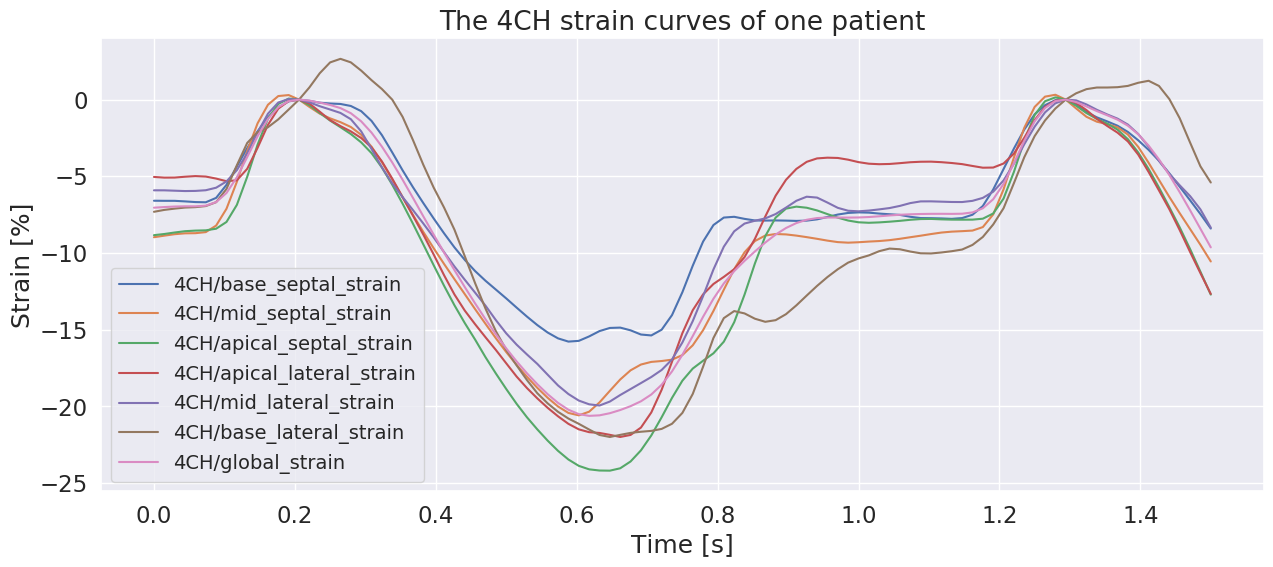
\includegraphics[width=0.95\textwidth]{data-exp/patient_strain_curves_4CH.png}
    %% Creator: Matplotlib, PGF backend
%%
%% To include the figure in your LaTeX document, write
%%   \input{<filename>.pgf}
%%
%% Make sure the required packages are loaded in your preamble
%%   \usepackage{pgf}
%%
%% Figures using additional raster images can only be included by \input if
%% they are in the same directory as the main LaTeX file. For loading figures
%% from other directories you can use the `import` package
%%   \usepackage{import}
%% and then include the figures with
%%   \import{<path to file>}{<filename>.pgf}
%%
%% Matplotlib used the following preamble
%%
\begingroup%
\makeatletter%
\begin{pgfpicture}%
\pgfpathrectangle{\pgfpointorigin}{\pgfqpoint{5.884489in}{2.980388in}}%
\pgfusepath{use as bounding box, clip}%
\begin{pgfscope}%
\pgfsetbuttcap%
\pgfsetmiterjoin%
\definecolor{currentfill}{rgb}{1.000000,1.000000,1.000000}%
\pgfsetfillcolor{currentfill}%
\pgfsetlinewidth{0.000000pt}%
\definecolor{currentstroke}{rgb}{1.000000,1.000000,1.000000}%
\pgfsetstrokecolor{currentstroke}%
\pgfsetdash{}{0pt}%
\pgfpathmoveto{\pgfqpoint{0.000000in}{0.000000in}}%
\pgfpathlineto{\pgfqpoint{5.884489in}{0.000000in}}%
\pgfpathlineto{\pgfqpoint{5.884489in}{2.980388in}}%
\pgfpathlineto{\pgfqpoint{0.000000in}{2.980388in}}%
\pgfpathclose%
\pgfusepath{fill}%
\end{pgfscope}%
\begin{pgfscope}%
\pgfsetbuttcap%
\pgfsetmiterjoin%
\definecolor{currentfill}{rgb}{0.917647,0.917647,0.949020}%
\pgfsetfillcolor{currentfill}%
\pgfsetlinewidth{0.000000pt}%
\definecolor{currentstroke}{rgb}{0.000000,0.000000,0.000000}%
\pgfsetstrokecolor{currentstroke}%
\pgfsetstrokeopacity{0.000000}%
\pgfsetdash{}{0pt}%
\pgfpathmoveto{\pgfqpoint{0.746989in}{0.602314in}}%
\pgfpathlineto{\pgfqpoint{5.784489in}{0.602314in}}%
\pgfpathlineto{\pgfqpoint{5.784489in}{2.681314in}}%
\pgfpathlineto{\pgfqpoint{0.746989in}{2.681314in}}%
\pgfpathclose%
\pgfusepath{fill}%
\end{pgfscope}%
\begin{pgfscope}%
\pgfpathrectangle{\pgfqpoint{0.746989in}{0.602314in}}{\pgfqpoint{5.037500in}{2.079000in}}%
\pgfusepath{clip}%
\pgfsetroundcap%
\pgfsetroundjoin%
\pgfsetlinewidth{1.003750pt}%
\definecolor{currentstroke}{rgb}{1.000000,1.000000,1.000000}%
\pgfsetstrokecolor{currentstroke}%
\pgfsetdash{}{0pt}%
\pgfpathmoveto{\pgfqpoint{0.975967in}{0.602314in}}%
\pgfpathlineto{\pgfqpoint{0.975967in}{2.681314in}}%
\pgfusepath{stroke}%
\end{pgfscope}%
\begin{pgfscope}%
\definecolor{textcolor}{rgb}{0.150000,0.150000,0.150000}%
\pgfsetstrokecolor{textcolor}%
\pgfsetfillcolor{textcolor}%
\pgftext[x=0.975967in,y=0.470370in,,top]{\color{textcolor}\sffamily\fontsize{12.000000}{14.400000}\selectfont \(\displaystyle 0.0\)}%
\end{pgfscope}%
\begin{pgfscope}%
\pgfpathrectangle{\pgfqpoint{0.746989in}{0.602314in}}{\pgfqpoint{5.037500in}{2.079000in}}%
\pgfusepath{clip}%
\pgfsetroundcap%
\pgfsetroundjoin%
\pgfsetlinewidth{1.003750pt}%
\definecolor{currentstroke}{rgb}{1.000000,1.000000,1.000000}%
\pgfsetstrokecolor{currentstroke}%
\pgfsetdash{}{0pt}%
\pgfpathmoveto{\pgfqpoint{1.586573in}{0.602314in}}%
\pgfpathlineto{\pgfqpoint{1.586573in}{2.681314in}}%
\pgfusepath{stroke}%
\end{pgfscope}%
\begin{pgfscope}%
\definecolor{textcolor}{rgb}{0.150000,0.150000,0.150000}%
\pgfsetstrokecolor{textcolor}%
\pgfsetfillcolor{textcolor}%
\pgftext[x=1.586573in,y=0.470370in,,top]{\color{textcolor}\sffamily\fontsize{12.000000}{14.400000}\selectfont \(\displaystyle 0.2\)}%
\end{pgfscope}%
\begin{pgfscope}%
\pgfpathrectangle{\pgfqpoint{0.746989in}{0.602314in}}{\pgfqpoint{5.037500in}{2.079000in}}%
\pgfusepath{clip}%
\pgfsetroundcap%
\pgfsetroundjoin%
\pgfsetlinewidth{1.003750pt}%
\definecolor{currentstroke}{rgb}{1.000000,1.000000,1.000000}%
\pgfsetstrokecolor{currentstroke}%
\pgfsetdash{}{0pt}%
\pgfpathmoveto{\pgfqpoint{2.197179in}{0.602314in}}%
\pgfpathlineto{\pgfqpoint{2.197179in}{2.681314in}}%
\pgfusepath{stroke}%
\end{pgfscope}%
\begin{pgfscope}%
\definecolor{textcolor}{rgb}{0.150000,0.150000,0.150000}%
\pgfsetstrokecolor{textcolor}%
\pgfsetfillcolor{textcolor}%
\pgftext[x=2.197179in,y=0.470370in,,top]{\color{textcolor}\sffamily\fontsize{12.000000}{14.400000}\selectfont \(\displaystyle 0.4\)}%
\end{pgfscope}%
\begin{pgfscope}%
\pgfpathrectangle{\pgfqpoint{0.746989in}{0.602314in}}{\pgfqpoint{5.037500in}{2.079000in}}%
\pgfusepath{clip}%
\pgfsetroundcap%
\pgfsetroundjoin%
\pgfsetlinewidth{1.003750pt}%
\definecolor{currentstroke}{rgb}{1.000000,1.000000,1.000000}%
\pgfsetstrokecolor{currentstroke}%
\pgfsetdash{}{0pt}%
\pgfpathmoveto{\pgfqpoint{2.807785in}{0.602314in}}%
\pgfpathlineto{\pgfqpoint{2.807785in}{2.681314in}}%
\pgfusepath{stroke}%
\end{pgfscope}%
\begin{pgfscope}%
\definecolor{textcolor}{rgb}{0.150000,0.150000,0.150000}%
\pgfsetstrokecolor{textcolor}%
\pgfsetfillcolor{textcolor}%
\pgftext[x=2.807785in,y=0.470370in,,top]{\color{textcolor}\sffamily\fontsize{12.000000}{14.400000}\selectfont \(\displaystyle 0.6\)}%
\end{pgfscope}%
\begin{pgfscope}%
\pgfpathrectangle{\pgfqpoint{0.746989in}{0.602314in}}{\pgfqpoint{5.037500in}{2.079000in}}%
\pgfusepath{clip}%
\pgfsetroundcap%
\pgfsetroundjoin%
\pgfsetlinewidth{1.003750pt}%
\definecolor{currentstroke}{rgb}{1.000000,1.000000,1.000000}%
\pgfsetstrokecolor{currentstroke}%
\pgfsetdash{}{0pt}%
\pgfpathmoveto{\pgfqpoint{3.418391in}{0.602314in}}%
\pgfpathlineto{\pgfqpoint{3.418391in}{2.681314in}}%
\pgfusepath{stroke}%
\end{pgfscope}%
\begin{pgfscope}%
\definecolor{textcolor}{rgb}{0.150000,0.150000,0.150000}%
\pgfsetstrokecolor{textcolor}%
\pgfsetfillcolor{textcolor}%
\pgftext[x=3.418391in,y=0.470370in,,top]{\color{textcolor}\sffamily\fontsize{12.000000}{14.400000}\selectfont \(\displaystyle 0.8\)}%
\end{pgfscope}%
\begin{pgfscope}%
\pgfpathrectangle{\pgfqpoint{0.746989in}{0.602314in}}{\pgfqpoint{5.037500in}{2.079000in}}%
\pgfusepath{clip}%
\pgfsetroundcap%
\pgfsetroundjoin%
\pgfsetlinewidth{1.003750pt}%
\definecolor{currentstroke}{rgb}{1.000000,1.000000,1.000000}%
\pgfsetstrokecolor{currentstroke}%
\pgfsetdash{}{0pt}%
\pgfpathmoveto{\pgfqpoint{4.028997in}{0.602314in}}%
\pgfpathlineto{\pgfqpoint{4.028997in}{2.681314in}}%
\pgfusepath{stroke}%
\end{pgfscope}%
\begin{pgfscope}%
\definecolor{textcolor}{rgb}{0.150000,0.150000,0.150000}%
\pgfsetstrokecolor{textcolor}%
\pgfsetfillcolor{textcolor}%
\pgftext[x=4.028997in,y=0.470370in,,top]{\color{textcolor}\sffamily\fontsize{12.000000}{14.400000}\selectfont \(\displaystyle 1.0\)}%
\end{pgfscope}%
\begin{pgfscope}%
\pgfpathrectangle{\pgfqpoint{0.746989in}{0.602314in}}{\pgfqpoint{5.037500in}{2.079000in}}%
\pgfusepath{clip}%
\pgfsetroundcap%
\pgfsetroundjoin%
\pgfsetlinewidth{1.003750pt}%
\definecolor{currentstroke}{rgb}{1.000000,1.000000,1.000000}%
\pgfsetstrokecolor{currentstroke}%
\pgfsetdash{}{0pt}%
\pgfpathmoveto{\pgfqpoint{4.639603in}{0.602314in}}%
\pgfpathlineto{\pgfqpoint{4.639603in}{2.681314in}}%
\pgfusepath{stroke}%
\end{pgfscope}%
\begin{pgfscope}%
\definecolor{textcolor}{rgb}{0.150000,0.150000,0.150000}%
\pgfsetstrokecolor{textcolor}%
\pgfsetfillcolor{textcolor}%
\pgftext[x=4.639603in,y=0.470370in,,top]{\color{textcolor}\sffamily\fontsize{12.000000}{14.400000}\selectfont \(\displaystyle 1.2\)}%
\end{pgfscope}%
\begin{pgfscope}%
\pgfpathrectangle{\pgfqpoint{0.746989in}{0.602314in}}{\pgfqpoint{5.037500in}{2.079000in}}%
\pgfusepath{clip}%
\pgfsetroundcap%
\pgfsetroundjoin%
\pgfsetlinewidth{1.003750pt}%
\definecolor{currentstroke}{rgb}{1.000000,1.000000,1.000000}%
\pgfsetstrokecolor{currentstroke}%
\pgfsetdash{}{0pt}%
\pgfpathmoveto{\pgfqpoint{5.250209in}{0.602314in}}%
\pgfpathlineto{\pgfqpoint{5.250209in}{2.681314in}}%
\pgfusepath{stroke}%
\end{pgfscope}%
\begin{pgfscope}%
\definecolor{textcolor}{rgb}{0.150000,0.150000,0.150000}%
\pgfsetstrokecolor{textcolor}%
\pgfsetfillcolor{textcolor}%
\pgftext[x=5.250209in,y=0.470370in,,top]{\color{textcolor}\sffamily\fontsize{12.000000}{14.400000}\selectfont \(\displaystyle 1.4\)}%
\end{pgfscope}%
\begin{pgfscope}%
\definecolor{textcolor}{rgb}{0.150000,0.150000,0.150000}%
\pgfsetstrokecolor{textcolor}%
\pgfsetfillcolor{textcolor}%
\pgftext[x=3.265739in,y=0.266667in,,top]{\color{textcolor}\sffamily\fontsize{12.000000}{14.400000}\selectfont Time [s]}%
\end{pgfscope}%
\begin{pgfscope}%
\pgfpathrectangle{\pgfqpoint{0.746989in}{0.602314in}}{\pgfqpoint{5.037500in}{2.079000in}}%
\pgfusepath{clip}%
\pgfsetroundcap%
\pgfsetroundjoin%
\pgfsetlinewidth{1.003750pt}%
\definecolor{currentstroke}{rgb}{1.000000,1.000000,1.000000}%
\pgfsetstrokecolor{currentstroke}%
\pgfsetdash{}{0pt}%
\pgfpathmoveto{\pgfqpoint{0.746989in}{0.639146in}}%
\pgfpathlineto{\pgfqpoint{5.784489in}{0.639146in}}%
\pgfusepath{stroke}%
\end{pgfscope}%
\begin{pgfscope}%
\definecolor{textcolor}{rgb}{0.150000,0.150000,0.150000}%
\pgfsetstrokecolor{textcolor}%
\pgfsetfillcolor{textcolor}%
\pgftext[x=0.322222in,y=0.581275in,left,base]{\color{textcolor}\sffamily\fontsize{12.000000}{14.400000}\selectfont \(\displaystyle -25\)}%
\end{pgfscope}%
\begin{pgfscope}%
\pgfpathrectangle{\pgfqpoint{0.746989in}{0.602314in}}{\pgfqpoint{5.037500in}{2.079000in}}%
\pgfusepath{clip}%
\pgfsetroundcap%
\pgfsetroundjoin%
\pgfsetlinewidth{1.003750pt}%
\definecolor{currentstroke}{rgb}{1.000000,1.000000,1.000000}%
\pgfsetstrokecolor{currentstroke}%
\pgfsetdash{}{0pt}%
\pgfpathmoveto{\pgfqpoint{0.746989in}{0.991268in}}%
\pgfpathlineto{\pgfqpoint{5.784489in}{0.991268in}}%
\pgfusepath{stroke}%
\end{pgfscope}%
\begin{pgfscope}%
\definecolor{textcolor}{rgb}{0.150000,0.150000,0.150000}%
\pgfsetstrokecolor{textcolor}%
\pgfsetfillcolor{textcolor}%
\pgftext[x=0.322222in,y=0.933398in,left,base]{\color{textcolor}\sffamily\fontsize{12.000000}{14.400000}\selectfont \(\displaystyle -20\)}%
\end{pgfscope}%
\begin{pgfscope}%
\pgfpathrectangle{\pgfqpoint{0.746989in}{0.602314in}}{\pgfqpoint{5.037500in}{2.079000in}}%
\pgfusepath{clip}%
\pgfsetroundcap%
\pgfsetroundjoin%
\pgfsetlinewidth{1.003750pt}%
\definecolor{currentstroke}{rgb}{1.000000,1.000000,1.000000}%
\pgfsetstrokecolor{currentstroke}%
\pgfsetdash{}{0pt}%
\pgfpathmoveto{\pgfqpoint{0.746989in}{1.343390in}}%
\pgfpathlineto{\pgfqpoint{5.784489in}{1.343390in}}%
\pgfusepath{stroke}%
\end{pgfscope}%
\begin{pgfscope}%
\definecolor{textcolor}{rgb}{0.150000,0.150000,0.150000}%
\pgfsetstrokecolor{textcolor}%
\pgfsetfillcolor{textcolor}%
\pgftext[x=0.322222in,y=1.285520in,left,base]{\color{textcolor}\sffamily\fontsize{12.000000}{14.400000}\selectfont \(\displaystyle -15\)}%
\end{pgfscope}%
\begin{pgfscope}%
\pgfpathrectangle{\pgfqpoint{0.746989in}{0.602314in}}{\pgfqpoint{5.037500in}{2.079000in}}%
\pgfusepath{clip}%
\pgfsetroundcap%
\pgfsetroundjoin%
\pgfsetlinewidth{1.003750pt}%
\definecolor{currentstroke}{rgb}{1.000000,1.000000,1.000000}%
\pgfsetstrokecolor{currentstroke}%
\pgfsetdash{}{0pt}%
\pgfpathmoveto{\pgfqpoint{0.746989in}{1.695512in}}%
\pgfpathlineto{\pgfqpoint{5.784489in}{1.695512in}}%
\pgfusepath{stroke}%
\end{pgfscope}%
\begin{pgfscope}%
\definecolor{textcolor}{rgb}{0.150000,0.150000,0.150000}%
\pgfsetstrokecolor{textcolor}%
\pgfsetfillcolor{textcolor}%
\pgftext[x=0.322222in,y=1.637642in,left,base]{\color{textcolor}\sffamily\fontsize{12.000000}{14.400000}\selectfont \(\displaystyle -10\)}%
\end{pgfscope}%
\begin{pgfscope}%
\pgfpathrectangle{\pgfqpoint{0.746989in}{0.602314in}}{\pgfqpoint{5.037500in}{2.079000in}}%
\pgfusepath{clip}%
\pgfsetroundcap%
\pgfsetroundjoin%
\pgfsetlinewidth{1.003750pt}%
\definecolor{currentstroke}{rgb}{1.000000,1.000000,1.000000}%
\pgfsetstrokecolor{currentstroke}%
\pgfsetdash{}{0pt}%
\pgfpathmoveto{\pgfqpoint{0.746989in}{2.047635in}}%
\pgfpathlineto{\pgfqpoint{5.784489in}{2.047635in}}%
\pgfusepath{stroke}%
\end{pgfscope}%
\begin{pgfscope}%
\definecolor{textcolor}{rgb}{0.150000,0.150000,0.150000}%
\pgfsetstrokecolor{textcolor}%
\pgfsetfillcolor{textcolor}%
\pgftext[x=0.403819in,y=1.989765in,left,base]{\color{textcolor}\sffamily\fontsize{12.000000}{14.400000}\selectfont \(\displaystyle -5\)}%
\end{pgfscope}%
\begin{pgfscope}%
\pgfpathrectangle{\pgfqpoint{0.746989in}{0.602314in}}{\pgfqpoint{5.037500in}{2.079000in}}%
\pgfusepath{clip}%
\pgfsetroundcap%
\pgfsetroundjoin%
\pgfsetlinewidth{1.003750pt}%
\definecolor{currentstroke}{rgb}{1.000000,1.000000,1.000000}%
\pgfsetstrokecolor{currentstroke}%
\pgfsetdash{}{0pt}%
\pgfpathmoveto{\pgfqpoint{0.746989in}{2.399757in}}%
\pgfpathlineto{\pgfqpoint{5.784489in}{2.399757in}}%
\pgfusepath{stroke}%
\end{pgfscope}%
\begin{pgfscope}%
\definecolor{textcolor}{rgb}{0.150000,0.150000,0.150000}%
\pgfsetstrokecolor{textcolor}%
\pgfsetfillcolor{textcolor}%
\pgftext[x=0.533449in,y=2.341887in,left,base]{\color{textcolor}\sffamily\fontsize{12.000000}{14.400000}\selectfont \(\displaystyle 0\)}%
\end{pgfscope}%
\begin{pgfscope}%
\definecolor{textcolor}{rgb}{0.150000,0.150000,0.150000}%
\pgfsetstrokecolor{textcolor}%
\pgfsetfillcolor{textcolor}%
\pgftext[x=0.266667in,y=1.641814in,,bottom,rotate=90.000000]{\color{textcolor}\sffamily\fontsize{12.000000}{14.400000}\selectfont Strain [\%]}%
\end{pgfscope}%
\begin{pgfscope}%
\pgfpathrectangle{\pgfqpoint{0.746989in}{0.602314in}}{\pgfqpoint{5.037500in}{2.079000in}}%
\pgfusepath{clip}%
\pgfsetroundcap%
\pgfsetroundjoin%
\pgfsetlinewidth{1.505625pt}%
\definecolor{currentstroke}{rgb}{0.298039,0.447059,0.690196}%
\pgfsetstrokecolor{currentstroke}%
\pgfsetdash{}{0pt}%
\pgfpathmoveto{\pgfqpoint{0.975967in}{1.935625in}}%
\pgfpathlineto{\pgfqpoint{1.020864in}{1.935229in}}%
\pgfpathlineto{\pgfqpoint{1.065762in}{1.935147in}}%
\pgfpathlineto{\pgfqpoint{1.110659in}{1.932573in}}%
\pgfpathlineto{\pgfqpoint{1.155557in}{1.929482in}}%
\pgfpathlineto{\pgfqpoint{1.200454in}{1.928507in}}%
\pgfpathlineto{\pgfqpoint{1.245352in}{1.948702in}}%
\pgfpathlineto{\pgfqpoint{1.290249in}{2.008638in}}%
\pgfpathlineto{\pgfqpoint{1.335147in}{2.093095in}}%
\pgfpathlineto{\pgfqpoint{1.380044in}{2.177026in}}%
\pgfpathlineto{\pgfqpoint{1.424942in}{2.254032in}}%
\pgfpathlineto{\pgfqpoint{1.469839in}{2.318606in}}%
\pgfpathlineto{\pgfqpoint{1.514737in}{2.364664in}}%
\pgfpathlineto{\pgfqpoint{1.559634in}{2.391490in}}%
\pgfpathlineto{\pgfqpoint{1.604532in}{2.399757in}}%
\pgfpathlineto{\pgfqpoint{1.649429in}{2.394144in}}%
\pgfpathlineto{\pgfqpoint{1.694327in}{2.385449in}}%
\pgfpathlineto{\pgfqpoint{1.739224in}{2.381812in}}%
\pgfpathlineto{\pgfqpoint{1.784122in}{2.379728in}}%
\pgfpathlineto{\pgfqpoint{1.829019in}{2.370514in}}%
\pgfpathlineto{\pgfqpoint{1.873917in}{2.346759in}}%
\pgfpathlineto{\pgfqpoint{1.918814in}{2.301898in}}%
\pgfpathlineto{\pgfqpoint{1.963712in}{2.236669in}}%
\pgfpathlineto{\pgfqpoint{2.008609in}{2.157149in}}%
\pgfpathlineto{\pgfqpoint{2.053507in}{2.074945in}}%
\pgfpathlineto{\pgfqpoint{2.098404in}{1.997518in}}%
\pgfpathlineto{\pgfqpoint{2.143302in}{1.924584in}}%
\pgfpathlineto{\pgfqpoint{2.188199in}{1.854020in}}%
\pgfpathlineto{\pgfqpoint{2.233097in}{1.786034in}}%
\pgfpathlineto{\pgfqpoint{2.277994in}{1.721663in}}%
\pgfpathlineto{\pgfqpoint{2.322892in}{1.664057in}}%
\pgfpathlineto{\pgfqpoint{2.367789in}{1.612639in}}%
\pgfpathlineto{\pgfqpoint{2.412687in}{1.568255in}}%
\pgfpathlineto{\pgfqpoint{2.457584in}{1.527820in}}%
\pgfpathlineto{\pgfqpoint{2.502482in}{1.487283in}}%
\pgfpathlineto{\pgfqpoint{2.547379in}{1.445193in}}%
\pgfpathlineto{\pgfqpoint{2.592277in}{1.403876in}}%
\pgfpathlineto{\pgfqpoint{2.637174in}{1.364956in}}%
\pgfpathlineto{\pgfqpoint{2.682072in}{1.330708in}}%
\pgfpathlineto{\pgfqpoint{2.726969in}{1.303911in}}%
\pgfpathlineto{\pgfqpoint{2.771867in}{1.289140in}}%
\pgfpathlineto{\pgfqpoint{2.816764in}{1.292481in}}%
\pgfpathlineto{\pgfqpoint{2.861662in}{1.312894in}}%
\pgfpathlineto{\pgfqpoint{2.906559in}{1.337316in}}%
\pgfpathlineto{\pgfqpoint{2.951457in}{1.351786in}}%
\pgfpathlineto{\pgfqpoint{2.996354in}{1.353339in}}%
\pgfpathlineto{\pgfqpoint{3.041252in}{1.340868in}}%
\pgfpathlineto{\pgfqpoint{3.086149in}{1.321614in}}%
\pgfpathlineto{\pgfqpoint{3.131047in}{1.317361in}}%
\pgfpathlineto{\pgfqpoint{3.175944in}{1.343690in}}%
\pgfpathlineto{\pgfqpoint{3.220842in}{1.410790in}}%
\pgfpathlineto{\pgfqpoint{3.265739in}{1.515735in}}%
\pgfpathlineto{\pgfqpoint{3.310637in}{1.637409in}}%
\pgfpathlineto{\pgfqpoint{3.355534in}{1.748329in}}%
\pgfpathlineto{\pgfqpoint{3.400432in}{1.824085in}}%
\pgfpathlineto{\pgfqpoint{3.445329in}{1.858365in}}%
\pgfpathlineto{\pgfqpoint{3.490227in}{1.861883in}}%
\pgfpathlineto{\pgfqpoint{3.535124in}{1.852408in}}%
\pgfpathlineto{\pgfqpoint{3.580022in}{1.845097in}}%
\pgfpathlineto{\pgfqpoint{3.624919in}{1.844525in}}%
\pgfpathlineto{\pgfqpoint{3.669817in}{1.845210in}}%
\pgfpathlineto{\pgfqpoint{3.714714in}{1.844388in}}%
\pgfpathlineto{\pgfqpoint{3.759612in}{1.843039in}}%
\pgfpathlineto{\pgfqpoint{3.804509in}{1.844378in}}%
\pgfpathlineto{\pgfqpoint{3.849407in}{1.850163in}}%
\pgfpathlineto{\pgfqpoint{3.894305in}{1.860944in}}%
\pgfpathlineto{\pgfqpoint{3.939202in}{1.872222in}}%
\pgfpathlineto{\pgfqpoint{3.984100in}{1.879570in}}%
\pgfpathlineto{\pgfqpoint{4.028997in}{1.882184in}}%
\pgfpathlineto{\pgfqpoint{4.073895in}{1.880942in}}%
\pgfpathlineto{\pgfqpoint{4.118792in}{1.876696in}}%
\pgfpathlineto{\pgfqpoint{4.163690in}{1.873561in}}%
\pgfpathlineto{\pgfqpoint{4.208587in}{1.870568in}}%
\pgfpathlineto{\pgfqpoint{4.253485in}{1.861922in}}%
\pgfpathlineto{\pgfqpoint{4.298382in}{1.856067in}}%
\pgfpathlineto{\pgfqpoint{4.343280in}{1.855535in}}%
\pgfpathlineto{\pgfqpoint{4.388177in}{1.854411in}}%
\pgfpathlineto{\pgfqpoint{4.433075in}{1.852485in}}%
\pgfpathlineto{\pgfqpoint{4.477972in}{1.856022in}}%
\pgfpathlineto{\pgfqpoint{4.522870in}{1.871344in}}%
\pgfpathlineto{\pgfqpoint{4.567767in}{1.911442in}}%
\pgfpathlineto{\pgfqpoint{4.612665in}{1.987140in}}%
\pgfpathlineto{\pgfqpoint{4.657562in}{2.081053in}}%
\pgfpathlineto{\pgfqpoint{4.702460in}{2.175020in}}%
\pgfpathlineto{\pgfqpoint{4.747357in}{2.262353in}}%
\pgfpathlineto{\pgfqpoint{4.792255in}{2.331983in}}%
\pgfpathlineto{\pgfqpoint{4.837152in}{2.373975in}}%
\pgfpathlineto{\pgfqpoint{4.882050in}{2.397146in}}%
\pgfpathlineto{\pgfqpoint{4.926947in}{2.399757in}}%
\pgfpathlineto{\pgfqpoint{4.971845in}{2.375906in}}%
\pgfpathlineto{\pgfqpoint{5.016742in}{2.342752in}}%
\pgfpathlineto{\pgfqpoint{5.061640in}{2.318425in}}%
\pgfpathlineto{\pgfqpoint{5.106537in}{2.299775in}}%
\pgfpathlineto{\pgfqpoint{5.151435in}{2.279830in}}%
\pgfpathlineto{\pgfqpoint{5.196332in}{2.251343in}}%
\pgfpathlineto{\pgfqpoint{5.241230in}{2.212886in}}%
\pgfpathlineto{\pgfqpoint{5.286127in}{2.169048in}}%
\pgfpathlineto{\pgfqpoint{5.331025in}{2.119148in}}%
\pgfpathlineto{\pgfqpoint{5.375922in}{2.061213in}}%
\pgfpathlineto{\pgfqpoint{5.420820in}{2.000026in}}%
\pgfpathlineto{\pgfqpoint{5.465717in}{1.937919in}}%
\pgfpathlineto{\pgfqpoint{5.510615in}{1.874453in}}%
\pgfpathlineto{\pgfqpoint{5.555512in}{1.807970in}}%
\pgfusepath{stroke}%
\end{pgfscope}%
\begin{pgfscope}%
\pgfpathrectangle{\pgfqpoint{0.746989in}{0.602314in}}{\pgfqpoint{5.037500in}{2.079000in}}%
\pgfusepath{clip}%
\pgfsetroundcap%
\pgfsetroundjoin%
\pgfsetlinewidth{1.505625pt}%
\definecolor{currentstroke}{rgb}{0.866667,0.517647,0.321569}%
\pgfsetstrokecolor{currentstroke}%
\pgfsetdash{}{0pt}%
\pgfpathmoveto{\pgfqpoint{0.975967in}{1.768078in}}%
\pgfpathlineto{\pgfqpoint{1.020864in}{1.775376in}}%
\pgfpathlineto{\pgfqpoint{1.065762in}{1.782065in}}%
\pgfpathlineto{\pgfqpoint{1.110659in}{1.786045in}}%
\pgfpathlineto{\pgfqpoint{1.155557in}{1.786663in}}%
\pgfpathlineto{\pgfqpoint{1.200454in}{1.791584in}}%
\pgfpathlineto{\pgfqpoint{1.245352in}{1.821525in}}%
\pgfpathlineto{\pgfqpoint{1.290249in}{1.898872in}}%
\pgfpathlineto{\pgfqpoint{1.335147in}{2.022345in}}%
\pgfpathlineto{\pgfqpoint{1.380044in}{2.164183in}}%
\pgfpathlineto{\pgfqpoint{1.424942in}{2.290751in}}%
\pgfpathlineto{\pgfqpoint{1.469839in}{2.376070in}}%
\pgfpathlineto{\pgfqpoint{1.514737in}{2.416061in}}%
\pgfpathlineto{\pgfqpoint{1.559634in}{2.420538in}}%
\pgfpathlineto{\pgfqpoint{1.604532in}{2.399757in}}%
\pgfpathlineto{\pgfqpoint{1.649429in}{2.366409in}}%
\pgfpathlineto{\pgfqpoint{1.694327in}{2.335387in}}%
\pgfpathlineto{\pgfqpoint{1.739224in}{2.313690in}}%
\pgfpathlineto{\pgfqpoint{1.784122in}{2.296164in}}%
\pgfpathlineto{\pgfqpoint{1.829019in}{2.274086in}}%
\pgfpathlineto{\pgfqpoint{1.873917in}{2.238282in}}%
\pgfpathlineto{\pgfqpoint{1.918814in}{2.183621in}}%
\pgfpathlineto{\pgfqpoint{1.963712in}{2.112591in}}%
\pgfpathlineto{\pgfqpoint{2.008609in}{2.032851in}}%
\pgfpathlineto{\pgfqpoint{2.053507in}{1.950950in}}%
\pgfpathlineto{\pgfqpoint{2.098404in}{1.870148in}}%
\pgfpathlineto{\pgfqpoint{2.143302in}{1.792162in}}%
\pgfpathlineto{\pgfqpoint{2.188199in}{1.717453in}}%
\pgfpathlineto{\pgfqpoint{2.233097in}{1.645435in}}%
\pgfpathlineto{\pgfqpoint{2.277994in}{1.575748in}}%
\pgfpathlineto{\pgfqpoint{2.322892in}{1.506857in}}%
\pgfpathlineto{\pgfqpoint{2.367789in}{1.437858in}}%
\pgfpathlineto{\pgfqpoint{2.412687in}{1.370597in}}%
\pgfpathlineto{\pgfqpoint{2.457584in}{1.304557in}}%
\pgfpathlineto{\pgfqpoint{2.502482in}{1.241173in}}%
\pgfpathlineto{\pgfqpoint{2.547379in}{1.182165in}}%
\pgfpathlineto{\pgfqpoint{2.592277in}{1.127723in}}%
\pgfpathlineto{\pgfqpoint{2.637174in}{1.076932in}}%
\pgfpathlineto{\pgfqpoint{2.682072in}{1.031118in}}%
\pgfpathlineto{\pgfqpoint{2.726969in}{0.991362in}}%
\pgfpathlineto{\pgfqpoint{2.771867in}{0.961771in}}%
\pgfpathlineto{\pgfqpoint{2.816764in}{0.950618in}}%
\pgfpathlineto{\pgfqpoint{2.861662in}{0.967423in}}%
\pgfpathlineto{\pgfqpoint{2.906559in}{1.009895in}}%
\pgfpathlineto{\pgfqpoint{2.951457in}{1.063135in}}%
\pgfpathlineto{\pgfqpoint{2.996354in}{1.115178in}}%
\pgfpathlineto{\pgfqpoint{3.041252in}{1.157281in}}%
\pgfpathlineto{\pgfqpoint{3.086149in}{1.183852in}}%
\pgfpathlineto{\pgfqpoint{3.131047in}{1.195966in}}%
\pgfpathlineto{\pgfqpoint{3.175944in}{1.200014in}}%
\pgfpathlineto{\pgfqpoint{3.220842in}{1.206234in}}%
\pgfpathlineto{\pgfqpoint{3.265739in}{1.227142in}}%
\pgfpathlineto{\pgfqpoint{3.310637in}{1.272050in}}%
\pgfpathlineto{\pgfqpoint{3.355534in}{1.341551in}}%
\pgfpathlineto{\pgfqpoint{3.400432in}{1.429948in}}%
\pgfpathlineto{\pgfqpoint{3.445329in}{1.527297in}}%
\pgfpathlineto{\pgfqpoint{3.490227in}{1.621306in}}%
\pgfpathlineto{\pgfqpoint{3.535124in}{1.698940in}}%
\pgfpathlineto{\pgfqpoint{3.580022in}{1.750622in}}%
\pgfpathlineto{\pgfqpoint{3.624919in}{1.775745in}}%
\pgfpathlineto{\pgfqpoint{3.669817in}{1.782912in}}%
\pgfpathlineto{\pgfqpoint{3.714714in}{1.781075in}}%
\pgfpathlineto{\pgfqpoint{3.759612in}{1.775580in}}%
\pgfpathlineto{\pgfqpoint{3.804509in}{1.768555in}}%
\pgfpathlineto{\pgfqpoint{3.849407in}{1.760840in}}%
\pgfpathlineto{\pgfqpoint{3.894305in}{1.752565in}}%
\pgfpathlineto{\pgfqpoint{3.939202in}{1.745741in}}%
\pgfpathlineto{\pgfqpoint{3.984100in}{1.743132in}}%
\pgfpathlineto{\pgfqpoint{4.028997in}{1.745104in}}%
\pgfpathlineto{\pgfqpoint{4.073895in}{1.748186in}}%
\pgfpathlineto{\pgfqpoint{4.118792in}{1.750595in}}%
\pgfpathlineto{\pgfqpoint{4.163690in}{1.754758in}}%
\pgfpathlineto{\pgfqpoint{4.208587in}{1.760944in}}%
\pgfpathlineto{\pgfqpoint{4.253485in}{1.768160in}}%
\pgfpathlineto{\pgfqpoint{4.298382in}{1.775143in}}%
\pgfpathlineto{\pgfqpoint{4.343280in}{1.782677in}}%
\pgfpathlineto{\pgfqpoint{4.388177in}{1.789559in}}%
\pgfpathlineto{\pgfqpoint{4.433075in}{1.793779in}}%
\pgfpathlineto{\pgfqpoint{4.477972in}{1.795986in}}%
\pgfpathlineto{\pgfqpoint{4.522870in}{1.798644in}}%
\pgfpathlineto{\pgfqpoint{4.567767in}{1.814688in}}%
\pgfpathlineto{\pgfqpoint{4.612665in}{1.872763in}}%
\pgfpathlineto{\pgfqpoint{4.657562in}{1.987969in}}%
\pgfpathlineto{\pgfqpoint{4.702460in}{2.133940in}}%
\pgfpathlineto{\pgfqpoint{4.747357in}{2.270343in}}%
\pgfpathlineto{\pgfqpoint{4.792255in}{2.366073in}}%
\pgfpathlineto{\pgfqpoint{4.837152in}{2.413333in}}%
\pgfpathlineto{\pgfqpoint{4.882050in}{2.421957in}}%
\pgfpathlineto{\pgfqpoint{4.926947in}{2.399757in}}%
\pgfpathlineto{\pgfqpoint{4.971845in}{2.359327in}}%
\pgfpathlineto{\pgfqpoint{5.016742in}{2.320833in}}%
\pgfpathlineto{\pgfqpoint{5.061640in}{2.298386in}}%
\pgfpathlineto{\pgfqpoint{5.106537in}{2.287265in}}%
\pgfpathlineto{\pgfqpoint{5.151435in}{2.272619in}}%
\pgfpathlineto{\pgfqpoint{5.196332in}{2.239183in}}%
\pgfpathlineto{\pgfqpoint{5.241230in}{2.182539in}}%
\pgfpathlineto{\pgfqpoint{5.286127in}{2.109745in}}%
\pgfpathlineto{\pgfqpoint{5.331025in}{2.031203in}}%
\pgfpathlineto{\pgfqpoint{5.375922in}{1.953059in}}%
\pgfpathlineto{\pgfqpoint{5.420820in}{1.878505in}}%
\pgfpathlineto{\pgfqpoint{5.465717in}{1.805973in}}%
\pgfpathlineto{\pgfqpoint{5.510615in}{1.733373in}}%
\pgfpathlineto{\pgfqpoint{5.555512in}{1.656878in}}%
\pgfusepath{stroke}%
\end{pgfscope}%
\begin{pgfscope}%
\pgfpathrectangle{\pgfqpoint{0.746989in}{0.602314in}}{\pgfqpoint{5.037500in}{2.079000in}}%
\pgfusepath{clip}%
\pgfsetroundcap%
\pgfsetroundjoin%
\pgfsetlinewidth{1.505625pt}%
\definecolor{currentstroke}{rgb}{0.333333,0.658824,0.407843}%
\pgfsetstrokecolor{currentstroke}%
\pgfsetdash{}{0pt}%
\pgfpathmoveto{\pgfqpoint{0.975967in}{1.777575in}}%
\pgfpathlineto{\pgfqpoint{1.020864in}{1.782909in}}%
\pgfpathlineto{\pgfqpoint{1.065762in}{1.789829in}}%
\pgfpathlineto{\pgfqpoint{1.110659in}{1.795815in}}%
\pgfpathlineto{\pgfqpoint{1.155557in}{1.798520in}}%
\pgfpathlineto{\pgfqpoint{1.200454in}{1.799722in}}%
\pgfpathlineto{\pgfqpoint{1.245352in}{1.807194in}}%
\pgfpathlineto{\pgfqpoint{1.290249in}{1.838204in}}%
\pgfpathlineto{\pgfqpoint{1.335147in}{1.916460in}}%
\pgfpathlineto{\pgfqpoint{1.380044in}{2.045610in}}%
\pgfpathlineto{\pgfqpoint{1.424942in}{2.192851in}}%
\pgfpathlineto{\pgfqpoint{1.469839in}{2.312170in}}%
\pgfpathlineto{\pgfqpoint{1.514737in}{2.379636in}}%
\pgfpathlineto{\pgfqpoint{1.559634in}{2.404446in}}%
\pgfpathlineto{\pgfqpoint{1.604532in}{2.399757in}}%
\pgfpathlineto{\pgfqpoint{1.649429in}{2.373709in}}%
\pgfpathlineto{\pgfqpoint{1.694327in}{2.338215in}}%
\pgfpathlineto{\pgfqpoint{1.739224in}{2.303492in}}%
\pgfpathlineto{\pgfqpoint{1.784122in}{2.273076in}}%
\pgfpathlineto{\pgfqpoint{1.829019in}{2.241677in}}%
\pgfpathlineto{\pgfqpoint{1.873917in}{2.203376in}}%
\pgfpathlineto{\pgfqpoint{1.918814in}{2.154041in}}%
\pgfpathlineto{\pgfqpoint{1.963712in}{2.087931in}}%
\pgfpathlineto{\pgfqpoint{2.008609in}{2.008921in}}%
\pgfpathlineto{\pgfqpoint{2.053507in}{1.921861in}}%
\pgfpathlineto{\pgfqpoint{2.098404in}{1.829956in}}%
\pgfpathlineto{\pgfqpoint{2.143302in}{1.734836in}}%
\pgfpathlineto{\pgfqpoint{2.188199in}{1.639283in}}%
\pgfpathlineto{\pgfqpoint{2.233097in}{1.545378in}}%
\pgfpathlineto{\pgfqpoint{2.277994in}{1.456000in}}%
\pgfpathlineto{\pgfqpoint{2.322892in}{1.374108in}}%
\pgfpathlineto{\pgfqpoint{2.367789in}{1.298008in}}%
\pgfpathlineto{\pgfqpoint{2.412687in}{1.217397in}}%
\pgfpathlineto{\pgfqpoint{2.457584in}{1.142785in}}%
\pgfpathlineto{\pgfqpoint{2.502482in}{1.071553in}}%
\pgfpathlineto{\pgfqpoint{2.547379in}{1.003637in}}%
\pgfpathlineto{\pgfqpoint{2.592277in}{0.941810in}}%
\pgfpathlineto{\pgfqpoint{2.637174in}{0.886199in}}%
\pgfpathlineto{\pgfqpoint{2.682072in}{0.834450in}}%
\pgfpathlineto{\pgfqpoint{2.726969in}{0.787643in}}%
\pgfpathlineto{\pgfqpoint{2.771867in}{0.748030in}}%
\pgfpathlineto{\pgfqpoint{2.816764in}{0.718895in}}%
\pgfpathlineto{\pgfqpoint{2.861662in}{0.702891in}}%
\pgfpathlineto{\pgfqpoint{2.906559in}{0.697461in}}%
\pgfpathlineto{\pgfqpoint{2.951457in}{0.696814in}}%
\pgfpathlineto{\pgfqpoint{2.996354in}{0.707684in}}%
\pgfpathlineto{\pgfqpoint{3.041252in}{0.738936in}}%
\pgfpathlineto{\pgfqpoint{3.086149in}{0.789874in}}%
\pgfpathlineto{\pgfqpoint{3.131047in}{0.858414in}}%
\pgfpathlineto{\pgfqpoint{3.175944in}{0.941952in}}%
\pgfpathlineto{\pgfqpoint{3.220842in}{1.030820in}}%
\pgfpathlineto{\pgfqpoint{3.265739in}{1.109620in}}%
\pgfpathlineto{\pgfqpoint{3.310637in}{1.165347in}}%
\pgfpathlineto{\pgfqpoint{3.355534in}{1.201303in}}%
\pgfpathlineto{\pgfqpoint{3.400432in}{1.235446in}}%
\pgfpathlineto{\pgfqpoint{3.445329in}{1.288738in}}%
\pgfpathlineto{\pgfqpoint{3.490227in}{1.377963in}}%
\pgfpathlineto{\pgfqpoint{3.535124in}{1.504757in}}%
\pgfpathlineto{\pgfqpoint{3.580022in}{1.647656in}}%
\pgfpathlineto{\pgfqpoint{3.624919in}{1.772771in}}%
\pgfpathlineto{\pgfqpoint{3.669817in}{1.858130in}}%
\pgfpathlineto{\pgfqpoint{3.714714in}{1.899425in}}%
\pgfpathlineto{\pgfqpoint{3.759612in}{1.908529in}}%
\pgfpathlineto{\pgfqpoint{3.804509in}{1.903475in}}%
\pgfpathlineto{\pgfqpoint{3.849407in}{1.891114in}}%
\pgfpathlineto{\pgfqpoint{3.894305in}{1.874259in}}%
\pgfpathlineto{\pgfqpoint{3.939202in}{1.857977in}}%
\pgfpathlineto{\pgfqpoint{3.984100in}{1.844677in}}%
\pgfpathlineto{\pgfqpoint{4.028997in}{1.836688in}}%
\pgfpathlineto{\pgfqpoint{4.073895in}{1.834390in}}%
\pgfpathlineto{\pgfqpoint{4.118792in}{1.836198in}}%
\pgfpathlineto{\pgfqpoint{4.163690in}{1.839421in}}%
\pgfpathlineto{\pgfqpoint{4.208587in}{1.843362in}}%
\pgfpathlineto{\pgfqpoint{4.253485in}{1.848145in}}%
\pgfpathlineto{\pgfqpoint{4.298382in}{1.851490in}}%
\pgfpathlineto{\pgfqpoint{4.343280in}{1.852157in}}%
\pgfpathlineto{\pgfqpoint{4.388177in}{1.850153in}}%
\pgfpathlineto{\pgfqpoint{4.433075in}{1.848870in}}%
\pgfpathlineto{\pgfqpoint{4.477972in}{1.848670in}}%
\pgfpathlineto{\pgfqpoint{4.522870in}{1.848865in}}%
\pgfpathlineto{\pgfqpoint{4.567767in}{1.853210in}}%
\pgfpathlineto{\pgfqpoint{4.612665in}{1.876984in}}%
\pgfpathlineto{\pgfqpoint{4.657562in}{1.945648in}}%
\pgfpathlineto{\pgfqpoint{4.702460in}{2.068014in}}%
\pgfpathlineto{\pgfqpoint{4.747357in}{2.211952in}}%
\pgfpathlineto{\pgfqpoint{4.792255in}{2.329182in}}%
\pgfpathlineto{\pgfqpoint{4.837152in}{2.392191in}}%
\pgfpathlineto{\pgfqpoint{4.882050in}{2.409948in}}%
\pgfpathlineto{\pgfqpoint{4.926947in}{2.399757in}}%
\pgfpathlineto{\pgfqpoint{4.971845in}{2.371910in}}%
\pgfpathlineto{\pgfqpoint{5.016742in}{2.338040in}}%
\pgfpathlineto{\pgfqpoint{5.061640in}{2.311135in}}%
\pgfpathlineto{\pgfqpoint{5.106537in}{2.289540in}}%
\pgfpathlineto{\pgfqpoint{5.151435in}{2.261936in}}%
\pgfpathlineto{\pgfqpoint{5.196332in}{2.218103in}}%
\pgfpathlineto{\pgfqpoint{5.241230in}{2.156942in}}%
\pgfpathlineto{\pgfqpoint{5.286127in}{2.081237in}}%
\pgfpathlineto{\pgfqpoint{5.331025in}{1.996106in}}%
\pgfpathlineto{\pgfqpoint{5.375922in}{1.905960in}}%
\pgfpathlineto{\pgfqpoint{5.420820in}{1.813412in}}%
\pgfpathlineto{\pgfqpoint{5.465717in}{1.714193in}}%
\pgfpathlineto{\pgfqpoint{5.510615in}{1.609982in}}%
\pgfpathlineto{\pgfqpoint{5.555512in}{1.504727in}}%
\pgfusepath{stroke}%
\end{pgfscope}%
\begin{pgfscope}%
\pgfpathrectangle{\pgfqpoint{0.746989in}{0.602314in}}{\pgfqpoint{5.037500in}{2.079000in}}%
\pgfusepath{clip}%
\pgfsetroundcap%
\pgfsetroundjoin%
\pgfsetlinewidth{1.505625pt}%
\definecolor{currentstroke}{rgb}{0.768627,0.305882,0.321569}%
\pgfsetstrokecolor{currentstroke}%
\pgfsetdash{}{0pt}%
\pgfpathmoveto{\pgfqpoint{0.975967in}{2.044800in}}%
\pgfpathlineto{\pgfqpoint{1.020864in}{2.041670in}}%
\pgfpathlineto{\pgfqpoint{1.065762in}{2.041950in}}%
\pgfpathlineto{\pgfqpoint{1.110659in}{2.045783in}}%
\pgfpathlineto{\pgfqpoint{1.155557in}{2.048738in}}%
\pgfpathlineto{\pgfqpoint{1.200454in}{2.046520in}}%
\pgfpathlineto{\pgfqpoint{1.245352in}{2.037310in}}%
\pgfpathlineto{\pgfqpoint{1.290249in}{2.025132in}}%
\pgfpathlineto{\pgfqpoint{1.335147in}{2.029400in}}%
\pgfpathlineto{\pgfqpoint{1.380044in}{2.081976in}}%
\pgfpathlineto{\pgfqpoint{1.424942in}{2.178434in}}%
\pgfpathlineto{\pgfqpoint{1.469839in}{2.283771in}}%
\pgfpathlineto{\pgfqpoint{1.514737in}{2.358351in}}%
\pgfpathlineto{\pgfqpoint{1.559634in}{2.393236in}}%
\pgfpathlineto{\pgfqpoint{1.604532in}{2.399757in}}%
\pgfpathlineto{\pgfqpoint{1.649429in}{2.381593in}}%
\pgfpathlineto{\pgfqpoint{1.694327in}{2.344346in}}%
\pgfpathlineto{\pgfqpoint{1.739224in}{2.305493in}}%
\pgfpathlineto{\pgfqpoint{1.784122in}{2.278068in}}%
\pgfpathlineto{\pgfqpoint{1.829019in}{2.253903in}}%
\pgfpathlineto{\pgfqpoint{1.873917in}{2.223496in}}%
\pgfpathlineto{\pgfqpoint{1.918814in}{2.179785in}}%
\pgfpathlineto{\pgfqpoint{1.963712in}{2.115999in}}%
\pgfpathlineto{\pgfqpoint{2.008609in}{2.036917in}}%
\pgfpathlineto{\pgfqpoint{2.053507in}{1.952201in}}%
\pgfpathlineto{\pgfqpoint{2.098404in}{1.866917in}}%
\pgfpathlineto{\pgfqpoint{2.143302in}{1.780015in}}%
\pgfpathlineto{\pgfqpoint{2.188199in}{1.688557in}}%
\pgfpathlineto{\pgfqpoint{2.233097in}{1.593736in}}%
\pgfpathlineto{\pgfqpoint{2.277994in}{1.505452in}}%
\pgfpathlineto{\pgfqpoint{2.322892in}{1.431364in}}%
\pgfpathlineto{\pgfqpoint{2.367789in}{1.368601in}}%
\pgfpathlineto{\pgfqpoint{2.412687in}{1.308953in}}%
\pgfpathlineto{\pgfqpoint{2.457584in}{1.250760in}}%
\pgfpathlineto{\pgfqpoint{2.502482in}{1.189499in}}%
\pgfpathlineto{\pgfqpoint{2.547379in}{1.128751in}}%
\pgfpathlineto{\pgfqpoint{2.592277in}{1.075939in}}%
\pgfpathlineto{\pgfqpoint{2.637174in}{1.028530in}}%
\pgfpathlineto{\pgfqpoint{2.682072in}{0.985195in}}%
\pgfpathlineto{\pgfqpoint{2.726969in}{0.946218in}}%
\pgfpathlineto{\pgfqpoint{2.771867in}{0.911697in}}%
\pgfpathlineto{\pgfqpoint{2.816764in}{0.886483in}}%
\pgfpathlineto{\pgfqpoint{2.861662in}{0.873416in}}%
\pgfpathlineto{\pgfqpoint{2.906559in}{0.869944in}}%
\pgfpathlineto{\pgfqpoint{2.951457in}{0.861236in}}%
\pgfpathlineto{\pgfqpoint{2.996354in}{0.851447in}}%
\pgfpathlineto{\pgfqpoint{3.041252in}{0.860779in}}%
\pgfpathlineto{\pgfqpoint{3.086149in}{0.894515in}}%
\pgfpathlineto{\pgfqpoint{3.131047in}{0.963947in}}%
\pgfpathlineto{\pgfqpoint{3.175944in}{1.068090in}}%
\pgfpathlineto{\pgfqpoint{3.220842in}{1.196997in}}%
\pgfpathlineto{\pgfqpoint{3.265739in}{1.327752in}}%
\pgfpathlineto{\pgfqpoint{3.310637in}{1.433136in}}%
\pgfpathlineto{\pgfqpoint{3.355534in}{1.505930in}}%
\pgfpathlineto{\pgfqpoint{3.400432in}{1.553551in}}%
\pgfpathlineto{\pgfqpoint{3.445329in}{1.586098in}}%
\pgfpathlineto{\pgfqpoint{3.490227in}{1.621457in}}%
\pgfpathlineto{\pgfqpoint{3.535124in}{1.677079in}}%
\pgfpathlineto{\pgfqpoint{3.580022in}{1.760791in}}%
\pgfpathlineto{\pgfqpoint{3.624919in}{1.863037in}}%
\pgfpathlineto{\pgfqpoint{3.669817in}{1.958735in}}%
\pgfpathlineto{\pgfqpoint{3.714714in}{2.031628in}}%
\pgfpathlineto{\pgfqpoint{3.759612in}{2.081597in}}%
\pgfpathlineto{\pgfqpoint{3.804509in}{2.114145in}}%
\pgfpathlineto{\pgfqpoint{3.849407in}{2.129884in}}%
\pgfpathlineto{\pgfqpoint{3.894305in}{2.133209in}}%
\pgfpathlineto{\pgfqpoint{3.939202in}{2.131929in}}%
\pgfpathlineto{\pgfqpoint{3.984100in}{2.123990in}}%
\pgfpathlineto{\pgfqpoint{4.028997in}{2.112771in}}%
\pgfpathlineto{\pgfqpoint{4.073895in}{2.105556in}}%
\pgfpathlineto{\pgfqpoint{4.118792in}{2.103257in}}%
\pgfpathlineto{\pgfqpoint{4.163690in}{2.104373in}}%
\pgfpathlineto{\pgfqpoint{4.208587in}{2.108083in}}%
\pgfpathlineto{\pgfqpoint{4.253485in}{2.112272in}}%
\pgfpathlineto{\pgfqpoint{4.298382in}{2.114548in}}%
\pgfpathlineto{\pgfqpoint{4.343280in}{2.115026in}}%
\pgfpathlineto{\pgfqpoint{4.388177in}{2.112568in}}%
\pgfpathlineto{\pgfqpoint{4.433075in}{2.108745in}}%
\pgfpathlineto{\pgfqpoint{4.477972in}{2.103624in}}%
\pgfpathlineto{\pgfqpoint{4.522870in}{2.095158in}}%
\pgfpathlineto{\pgfqpoint{4.567767in}{2.087192in}}%
\pgfpathlineto{\pgfqpoint{4.612665in}{2.087896in}}%
\pgfpathlineto{\pgfqpoint{4.657562in}{2.106468in}}%
\pgfpathlineto{\pgfqpoint{4.702460in}{2.152026in}}%
\pgfpathlineto{\pgfqpoint{4.747357in}{2.224696in}}%
\pgfpathlineto{\pgfqpoint{4.792255in}{2.305497in}}%
\pgfpathlineto{\pgfqpoint{4.837152in}{2.365705in}}%
\pgfpathlineto{\pgfqpoint{4.882050in}{2.394890in}}%
\pgfpathlineto{\pgfqpoint{4.926947in}{2.399757in}}%
\pgfpathlineto{\pgfqpoint{4.971845in}{2.384724in}}%
\pgfpathlineto{\pgfqpoint{5.016742in}{2.351575in}}%
\pgfpathlineto{\pgfqpoint{5.061640in}{2.311992in}}%
\pgfpathlineto{\pgfqpoint{5.106537in}{2.278847in}}%
\pgfpathlineto{\pgfqpoint{5.151435in}{2.248017in}}%
\pgfpathlineto{\pgfqpoint{5.196332in}{2.207800in}}%
\pgfpathlineto{\pgfqpoint{5.241230in}{2.147093in}}%
\pgfpathlineto{\pgfqpoint{5.286127in}{2.067691in}}%
\pgfpathlineto{\pgfqpoint{5.331025in}{1.982889in}}%
\pgfpathlineto{\pgfqpoint{5.375922in}{1.896694in}}%
\pgfpathlineto{\pgfqpoint{5.420820in}{1.801061in}}%
\pgfpathlineto{\pgfqpoint{5.465717in}{1.700792in}}%
\pgfpathlineto{\pgfqpoint{5.510615in}{1.603379in}}%
\pgfpathlineto{\pgfqpoint{5.555512in}{1.507817in}}%
\pgfusepath{stroke}%
\end{pgfscope}%
\begin{pgfscope}%
\pgfpathrectangle{\pgfqpoint{0.746989in}{0.602314in}}{\pgfqpoint{5.037500in}{2.079000in}}%
\pgfusepath{clip}%
\pgfsetroundcap%
\pgfsetroundjoin%
\pgfsetlinewidth{1.505625pt}%
\definecolor{currentstroke}{rgb}{0.505882,0.447059,0.701961}%
\pgfsetstrokecolor{currentstroke}%
\pgfsetdash{}{0pt}%
\pgfpathmoveto{\pgfqpoint{0.975967in}{1.983403in}}%
\pgfpathlineto{\pgfqpoint{1.020864in}{1.983341in}}%
\pgfpathlineto{\pgfqpoint{1.065762in}{1.981658in}}%
\pgfpathlineto{\pgfqpoint{1.110659in}{1.980023in}}%
\pgfpathlineto{\pgfqpoint{1.155557in}{1.980677in}}%
\pgfpathlineto{\pgfqpoint{1.200454in}{1.983762in}}%
\pgfpathlineto{\pgfqpoint{1.245352in}{1.995403in}}%
\pgfpathlineto{\pgfqpoint{1.290249in}{2.024107in}}%
\pgfpathlineto{\pgfqpoint{1.335147in}{2.075882in}}%
\pgfpathlineto{\pgfqpoint{1.380044in}{2.153445in}}%
\pgfpathlineto{\pgfqpoint{1.424942in}{2.248432in}}%
\pgfpathlineto{\pgfqpoint{1.469839in}{2.334923in}}%
\pgfpathlineto{\pgfqpoint{1.514737in}{2.386375in}}%
\pgfpathlineto{\pgfqpoint{1.559634in}{2.402355in}}%
\pgfpathlineto{\pgfqpoint{1.604532in}{2.399757in}}%
\pgfpathlineto{\pgfqpoint{1.649429in}{2.387298in}}%
\pgfpathlineto{\pgfqpoint{1.694327in}{2.369467in}}%
\pgfpathlineto{\pgfqpoint{1.739224in}{2.354222in}}%
\pgfpathlineto{\pgfqpoint{1.784122in}{2.338514in}}%
\pgfpathlineto{\pgfqpoint{1.829019in}{2.309819in}}%
\pgfpathlineto{\pgfqpoint{1.873917in}{2.253972in}}%
\pgfpathlineto{\pgfqpoint{1.918814in}{2.173027in}}%
\pgfpathlineto{\pgfqpoint{1.963712in}{2.088909in}}%
\pgfpathlineto{\pgfqpoint{2.008609in}{2.014934in}}%
\pgfpathlineto{\pgfqpoint{2.053507in}{1.952063in}}%
\pgfpathlineto{\pgfqpoint{2.098404in}{1.892479in}}%
\pgfpathlineto{\pgfqpoint{2.143302in}{1.830903in}}%
\pgfpathlineto{\pgfqpoint{2.188199in}{1.767035in}}%
\pgfpathlineto{\pgfqpoint{2.233097in}{1.699622in}}%
\pgfpathlineto{\pgfqpoint{2.277994in}{1.633949in}}%
\pgfpathlineto{\pgfqpoint{2.322892in}{1.572944in}}%
\pgfpathlineto{\pgfqpoint{2.367789in}{1.513528in}}%
\pgfpathlineto{\pgfqpoint{2.412687in}{1.453823in}}%
\pgfpathlineto{\pgfqpoint{2.457584in}{1.387758in}}%
\pgfpathlineto{\pgfqpoint{2.502482in}{1.326919in}}%
\pgfpathlineto{\pgfqpoint{2.547379in}{1.275241in}}%
\pgfpathlineto{\pgfqpoint{2.592277in}{1.230145in}}%
\pgfpathlineto{\pgfqpoint{2.637174in}{1.186768in}}%
\pgfpathlineto{\pgfqpoint{2.682072in}{1.137068in}}%
\pgfpathlineto{\pgfqpoint{2.726969in}{1.087856in}}%
\pgfpathlineto{\pgfqpoint{2.771867in}{1.048500in}}%
\pgfpathlineto{\pgfqpoint{2.816764in}{1.018567in}}%
\pgfpathlineto{\pgfqpoint{2.861662in}{1.001368in}}%
\pgfpathlineto{\pgfqpoint{2.906559in}{0.995691in}}%
\pgfpathlineto{\pgfqpoint{2.951457in}{1.013973in}}%
\pgfpathlineto{\pgfqpoint{2.996354in}{1.043908in}}%
\pgfpathlineto{\pgfqpoint{3.041252in}{1.071315in}}%
\pgfpathlineto{\pgfqpoint{3.086149in}{1.098762in}}%
\pgfpathlineto{\pgfqpoint{3.131047in}{1.126537in}}%
\pgfpathlineto{\pgfqpoint{3.175944in}{1.158937in}}%
\pgfpathlineto{\pgfqpoint{3.220842in}{1.207115in}}%
\pgfpathlineto{\pgfqpoint{3.265739in}{1.285146in}}%
\pgfpathlineto{\pgfqpoint{3.310637in}{1.383104in}}%
\pgfpathlineto{\pgfqpoint{3.355534in}{1.498009in}}%
\pgfpathlineto{\pgfqpoint{3.400432in}{1.620311in}}%
\pgfpathlineto{\pgfqpoint{3.445329in}{1.724747in}}%
\pgfpathlineto{\pgfqpoint{3.490227in}{1.795258in}}%
\pgfpathlineto{\pgfqpoint{3.535124in}{1.830777in}}%
\pgfpathlineto{\pgfqpoint{3.580022in}{1.843823in}}%
\pgfpathlineto{\pgfqpoint{3.624919in}{1.854508in}}%
\pgfpathlineto{\pgfqpoint{3.669817in}{1.874444in}}%
\pgfpathlineto{\pgfqpoint{3.714714in}{1.903987in}}%
\pgfpathlineto{\pgfqpoint{3.759612in}{1.935380in}}%
\pgfpathlineto{\pgfqpoint{3.804509in}{1.954104in}}%
\pgfpathlineto{\pgfqpoint{3.849407in}{1.950069in}}%
\pgfpathlineto{\pgfqpoint{3.894305in}{1.927239in}}%
\pgfpathlineto{\pgfqpoint{3.939202in}{1.903003in}}%
\pgfpathlineto{\pgfqpoint{3.984100in}{1.889685in}}%
\pgfpathlineto{\pgfqpoint{4.028997in}{1.887021in}}%
\pgfpathlineto{\pgfqpoint{4.073895in}{1.890497in}}%
\pgfpathlineto{\pgfqpoint{4.118792in}{1.895878in}}%
\pgfpathlineto{\pgfqpoint{4.163690in}{1.902056in}}%
\pgfpathlineto{\pgfqpoint{4.208587in}{1.911952in}}%
\pgfpathlineto{\pgfqpoint{4.253485in}{1.924793in}}%
\pgfpathlineto{\pgfqpoint{4.298382in}{1.932570in}}%
\pgfpathlineto{\pgfqpoint{4.343280in}{1.932798in}}%
\pgfpathlineto{\pgfqpoint{4.388177in}{1.931342in}}%
\pgfpathlineto{\pgfqpoint{4.433075in}{1.929887in}}%
\pgfpathlineto{\pgfqpoint{4.477972in}{1.929601in}}%
\pgfpathlineto{\pgfqpoint{4.522870in}{1.935072in}}%
\pgfpathlineto{\pgfqpoint{4.567767in}{1.948711in}}%
\pgfpathlineto{\pgfqpoint{4.612665in}{1.977025in}}%
\pgfpathlineto{\pgfqpoint{4.657562in}{2.028754in}}%
\pgfpathlineto{\pgfqpoint{4.702460in}{2.105845in}}%
\pgfpathlineto{\pgfqpoint{4.747357in}{2.195030in}}%
\pgfpathlineto{\pgfqpoint{4.792255in}{2.275469in}}%
\pgfpathlineto{\pgfqpoint{4.837152in}{2.340991in}}%
\pgfpathlineto{\pgfqpoint{4.882050in}{2.382860in}}%
\pgfpathlineto{\pgfqpoint{4.926947in}{2.399757in}}%
\pgfpathlineto{\pgfqpoint{4.971845in}{2.396323in}}%
\pgfpathlineto{\pgfqpoint{5.016742in}{2.377551in}}%
\pgfpathlineto{\pgfqpoint{5.061640in}{2.353060in}}%
\pgfpathlineto{\pgfqpoint{5.106537in}{2.331633in}}%
\pgfpathlineto{\pgfqpoint{5.151435in}{2.312387in}}%
\pgfpathlineto{\pgfqpoint{5.196332in}{2.285099in}}%
\pgfpathlineto{\pgfqpoint{5.241230in}{2.241679in}}%
\pgfpathlineto{\pgfqpoint{5.286127in}{2.183607in}}%
\pgfpathlineto{\pgfqpoint{5.331025in}{2.118657in}}%
\pgfpathlineto{\pgfqpoint{5.375922in}{2.058399in}}%
\pgfpathlineto{\pgfqpoint{5.420820in}{2.006489in}}%
\pgfpathlineto{\pgfqpoint{5.465717in}{1.957136in}}%
\pgfpathlineto{\pgfqpoint{5.510615in}{1.895897in}}%
\pgfpathlineto{\pgfqpoint{5.555512in}{1.812257in}}%
\pgfusepath{stroke}%
\end{pgfscope}%
\begin{pgfscope}%
\pgfpathrectangle{\pgfqpoint{0.746989in}{0.602314in}}{\pgfqpoint{5.037500in}{2.079000in}}%
\pgfusepath{clip}%
\pgfsetroundcap%
\pgfsetroundjoin%
\pgfsetlinewidth{1.505625pt}%
\definecolor{currentstroke}{rgb}{0.576471,0.470588,0.376471}%
\pgfsetstrokecolor{currentstroke}%
\pgfsetdash{}{0pt}%
\pgfpathmoveto{\pgfqpoint{0.975967in}{1.884850in}}%
\pgfpathlineto{\pgfqpoint{1.020864in}{1.893536in}}%
\pgfpathlineto{\pgfqpoint{1.065762in}{1.899413in}}%
\pgfpathlineto{\pgfqpoint{1.110659in}{1.904307in}}%
\pgfpathlineto{\pgfqpoint{1.155557in}{1.906158in}}%
\pgfpathlineto{\pgfqpoint{1.200454in}{1.911097in}}%
\pgfpathlineto{\pgfqpoint{1.245352in}{1.928967in}}%
\pgfpathlineto{\pgfqpoint{1.290249in}{1.989709in}}%
\pgfpathlineto{\pgfqpoint{1.335147in}{2.098270in}}%
\pgfpathlineto{\pgfqpoint{1.380044in}{2.200851in}}%
\pgfpathlineto{\pgfqpoint{1.424942in}{2.250610in}}%
\pgfpathlineto{\pgfqpoint{1.469839in}{2.272848in}}%
\pgfpathlineto{\pgfqpoint{1.514737in}{2.309109in}}%
\pgfpathlineto{\pgfqpoint{1.559634in}{2.354089in}}%
\pgfpathlineto{\pgfqpoint{1.604532in}{2.399757in}}%
\pgfpathlineto{\pgfqpoint{1.649429in}{2.455503in}}%
\pgfpathlineto{\pgfqpoint{1.694327in}{2.520734in}}%
\pgfpathlineto{\pgfqpoint{1.739224in}{2.570410in}}%
\pgfpathlineto{\pgfqpoint{1.784122in}{2.586814in}}%
\pgfpathlineto{\pgfqpoint{1.829019in}{2.570630in}}%
\pgfpathlineto{\pgfqpoint{1.873917in}{2.532845in}}%
\pgfpathlineto{\pgfqpoint{1.918814in}{2.488842in}}%
\pgfpathlineto{\pgfqpoint{1.963712in}{2.448245in}}%
\pgfpathlineto{\pgfqpoint{2.008609in}{2.399454in}}%
\pgfpathlineto{\pgfqpoint{2.053507in}{2.320361in}}%
\pgfpathlineto{\pgfqpoint{2.098404in}{2.213800in}}%
\pgfpathlineto{\pgfqpoint{2.143302in}{2.100231in}}%
\pgfpathlineto{\pgfqpoint{2.188199in}{1.995592in}}%
\pgfpathlineto{\pgfqpoint{2.233097in}{1.904172in}}%
\pgfpathlineto{\pgfqpoint{2.277994in}{1.802905in}}%
\pgfpathlineto{\pgfqpoint{2.322892in}{1.680690in}}%
\pgfpathlineto{\pgfqpoint{2.367789in}{1.556721in}}%
\pgfpathlineto{\pgfqpoint{2.412687in}{1.440432in}}%
\pgfpathlineto{\pgfqpoint{2.457584in}{1.336906in}}%
\pgfpathlineto{\pgfqpoint{2.502482in}{1.251105in}}%
\pgfpathlineto{\pgfqpoint{2.547379in}{1.180374in}}%
\pgfpathlineto{\pgfqpoint{2.592277in}{1.112536in}}%
\pgfpathlineto{\pgfqpoint{2.637174in}{1.052208in}}%
\pgfpathlineto{\pgfqpoint{2.682072in}{1.005567in}}%
\pgfpathlineto{\pgfqpoint{2.726969in}{0.966825in}}%
\pgfpathlineto{\pgfqpoint{2.771867in}{0.936036in}}%
\pgfpathlineto{\pgfqpoint{2.816764in}{0.911836in}}%
\pgfpathlineto{\pgfqpoint{2.861662in}{0.885605in}}%
\pgfpathlineto{\pgfqpoint{2.906559in}{0.860635in}}%
\pgfpathlineto{\pgfqpoint{2.951457in}{0.851373in}}%
\pgfpathlineto{\pgfqpoint{2.996354in}{0.861069in}}%
\pgfpathlineto{\pgfqpoint{3.041252in}{0.870177in}}%
\pgfpathlineto{\pgfqpoint{3.086149in}{0.875409in}}%
\pgfpathlineto{\pgfqpoint{3.131047in}{0.879325in}}%
\pgfpathlineto{\pgfqpoint{3.175944in}{0.888443in}}%
\pgfpathlineto{\pgfqpoint{3.220842in}{0.912017in}}%
\pgfpathlineto{\pgfqpoint{3.265739in}{0.961739in}}%
\pgfpathlineto{\pgfqpoint{3.310637in}{1.048765in}}%
\pgfpathlineto{\pgfqpoint{3.355534in}{1.174006in}}%
\pgfpathlineto{\pgfqpoint{3.400432in}{1.305910in}}%
\pgfpathlineto{\pgfqpoint{3.445329in}{1.396792in}}%
\pgfpathlineto{\pgfqpoint{3.490227in}{1.429215in}}%
\pgfpathlineto{\pgfqpoint{3.535124in}{1.418443in}}%
\pgfpathlineto{\pgfqpoint{3.580022in}{1.394162in}}%
\pgfpathlineto{\pgfqpoint{3.624919in}{1.380002in}}%
\pgfpathlineto{\pgfqpoint{3.669817in}{1.387467in}}%
\pgfpathlineto{\pgfqpoint{3.714714in}{1.414953in}}%
\pgfpathlineto{\pgfqpoint{3.759612in}{1.455326in}}%
\pgfpathlineto{\pgfqpoint{3.804509in}{1.500486in}}%
\pgfpathlineto{\pgfqpoint{3.849407in}{1.544760in}}%
\pgfpathlineto{\pgfqpoint{3.894305in}{1.585336in}}%
\pgfpathlineto{\pgfqpoint{3.939202in}{1.621239in}}%
\pgfpathlineto{\pgfqpoint{3.984100in}{1.651635in}}%
\pgfpathlineto{\pgfqpoint{4.028997in}{1.670793in}}%
\pgfpathlineto{\pgfqpoint{4.073895in}{1.684783in}}%
\pgfpathlineto{\pgfqpoint{4.118792in}{1.704177in}}%
\pgfpathlineto{\pgfqpoint{4.163690in}{1.716050in}}%
\pgfpathlineto{\pgfqpoint{4.208587in}{1.712847in}}%
\pgfpathlineto{\pgfqpoint{4.253485in}{1.702383in}}%
\pgfpathlineto{\pgfqpoint{4.298382in}{1.694447in}}%
\pgfpathlineto{\pgfqpoint{4.343280in}{1.693582in}}%
\pgfpathlineto{\pgfqpoint{4.388177in}{1.698148in}}%
\pgfpathlineto{\pgfqpoint{4.433075in}{1.703979in}}%
\pgfpathlineto{\pgfqpoint{4.477972in}{1.711636in}}%
\pgfpathlineto{\pgfqpoint{4.522870in}{1.732823in}}%
\pgfpathlineto{\pgfqpoint{4.567767in}{1.769378in}}%
\pgfpathlineto{\pgfqpoint{4.612665in}{1.826644in}}%
\pgfpathlineto{\pgfqpoint{4.657562in}{1.901228in}}%
\pgfpathlineto{\pgfqpoint{4.702460in}{2.016444in}}%
\pgfpathlineto{\pgfqpoint{4.747357in}{2.135547in}}%
\pgfpathlineto{\pgfqpoint{4.792255in}{2.232241in}}%
\pgfpathlineto{\pgfqpoint{4.837152in}{2.303907in}}%
\pgfpathlineto{\pgfqpoint{4.882050in}{2.358766in}}%
\pgfpathlineto{\pgfqpoint{4.926947in}{2.399757in}}%
\pgfpathlineto{\pgfqpoint{4.971845in}{2.428553in}}%
\pgfpathlineto{\pgfqpoint{5.016742in}{2.447697in}}%
\pgfpathlineto{\pgfqpoint{5.061640in}{2.455169in}}%
\pgfpathlineto{\pgfqpoint{5.106537in}{2.455213in}}%
\pgfpathlineto{\pgfqpoint{5.151435in}{2.456726in}}%
\pgfpathlineto{\pgfqpoint{5.196332in}{2.462612in}}%
\pgfpathlineto{\pgfqpoint{5.241230in}{2.477001in}}%
\pgfpathlineto{\pgfqpoint{5.286127in}{2.486109in}}%
\pgfpathlineto{\pgfqpoint{5.331025in}{2.462394in}}%
\pgfpathlineto{\pgfqpoint{5.375922in}{2.402240in}}%
\pgfpathlineto{\pgfqpoint{5.420820in}{2.314257in}}%
\pgfpathlineto{\pgfqpoint{5.465717in}{2.202898in}}%
\pgfpathlineto{\pgfqpoint{5.510615in}{2.093493in}}%
\pgfpathlineto{\pgfqpoint{5.555512in}{2.019268in}}%
\pgfusepath{stroke}%
\end{pgfscope}%
\begin{pgfscope}%
\pgfpathrectangle{\pgfqpoint{0.746989in}{0.602314in}}{\pgfqpoint{5.037500in}{2.079000in}}%
\pgfusepath{clip}%
\pgfsetroundcap%
\pgfsetroundjoin%
\pgfsetlinewidth{1.505625pt}%
\definecolor{currentstroke}{rgb}{0.854902,0.545098,0.764706}%
\pgfsetstrokecolor{currentstroke}%
\pgfsetdash{}{0pt}%
\pgfpathmoveto{\pgfqpoint{0.975967in}{1.903659in}}%
\pgfpathlineto{\pgfqpoint{1.020864in}{1.906541in}}%
\pgfpathlineto{\pgfqpoint{1.065762in}{1.908948in}}%
\pgfpathlineto{\pgfqpoint{1.110659in}{1.910057in}}%
\pgfpathlineto{\pgfqpoint{1.155557in}{1.910012in}}%
\pgfpathlineto{\pgfqpoint{1.200454in}{1.912996in}}%
\pgfpathlineto{\pgfqpoint{1.245352in}{1.929271in}}%
\pgfpathlineto{\pgfqpoint{1.290249in}{1.971144in}}%
\pgfpathlineto{\pgfqpoint{1.335147in}{2.043091in}}%
\pgfpathlineto{\pgfqpoint{1.380044in}{2.135971in}}%
\pgfpathlineto{\pgfqpoint{1.424942in}{2.231209in}}%
\pgfpathlineto{\pgfqpoint{1.469839in}{2.310875in}}%
\pgfpathlineto{\pgfqpoint{1.514737in}{2.364891in}}%
\pgfpathlineto{\pgfqpoint{1.559634in}{2.392492in}}%
\pgfpathlineto{\pgfqpoint{1.604532in}{2.399757in}}%
\pgfpathlineto{\pgfqpoint{1.649429in}{2.395158in}}%
\pgfpathlineto{\pgfqpoint{1.694327in}{2.385907in}}%
\pgfpathlineto{\pgfqpoint{1.739224in}{2.375126in}}%
\pgfpathlineto{\pgfqpoint{1.784122in}{2.360766in}}%
\pgfpathlineto{\pgfqpoint{1.829019in}{2.337313in}}%
\pgfpathlineto{\pgfqpoint{1.873917in}{2.300033in}}%
\pgfpathlineto{\pgfqpoint{1.918814in}{2.248059in}}%
\pgfpathlineto{\pgfqpoint{1.963712in}{2.183970in}}%
\pgfpathlineto{\pgfqpoint{2.008609in}{2.111055in}}%
\pgfpathlineto{\pgfqpoint{2.053507in}{2.031774in}}%
\pgfpathlineto{\pgfqpoint{2.098404in}{1.948478in}}%
\pgfpathlineto{\pgfqpoint{2.143302in}{1.863787in}}%
\pgfpathlineto{\pgfqpoint{2.188199in}{1.779859in}}%
\pgfpathlineto{\pgfqpoint{2.233097in}{1.697685in}}%
\pgfpathlineto{\pgfqpoint{2.277994in}{1.617398in}}%
\pgfpathlineto{\pgfqpoint{2.322892in}{1.539360in}}%
\pgfpathlineto{\pgfqpoint{2.367789in}{1.464058in}}%
\pgfpathlineto{\pgfqpoint{2.412687in}{1.391552in}}%
\pgfpathlineto{\pgfqpoint{2.457584in}{1.322507in}}%
\pgfpathlineto{\pgfqpoint{2.502482in}{1.257909in}}%
\pgfpathlineto{\pgfqpoint{2.547379in}{1.198370in}}%
\pgfpathlineto{\pgfqpoint{2.592277in}{1.143725in}}%
\pgfpathlineto{\pgfqpoint{2.637174in}{1.093501in}}%
\pgfpathlineto{\pgfqpoint{2.682072in}{1.047750in}}%
\pgfpathlineto{\pgfqpoint{2.726969in}{1.007806in}}%
\pgfpathlineto{\pgfqpoint{2.771867in}{0.976430in}}%
\pgfpathlineto{\pgfqpoint{2.816764in}{0.956356in}}%
\pgfpathlineto{\pgfqpoint{2.861662in}{0.948349in}}%
\pgfpathlineto{\pgfqpoint{2.906559in}{0.950668in}}%
\pgfpathlineto{\pgfqpoint{2.951457in}{0.960454in}}%
\pgfpathlineto{\pgfqpoint{2.996354in}{0.975040in}}%
\pgfpathlineto{\pgfqpoint{3.041252in}{0.992805in}}%
\pgfpathlineto{\pgfqpoint{3.086149in}{1.015130in}}%
\pgfpathlineto{\pgfqpoint{3.131047in}{1.046312in}}%
\pgfpathlineto{\pgfqpoint{3.175944in}{1.091107in}}%
\pgfpathlineto{\pgfqpoint{3.220842in}{1.152290in}}%
\pgfpathlineto{\pgfqpoint{3.265739in}{1.228578in}}%
\pgfpathlineto{\pgfqpoint{3.310637in}{1.314535in}}%
\pgfpathlineto{\pgfqpoint{3.355534in}{1.403062in}}%
\pgfpathlineto{\pgfqpoint{3.400432in}{1.485898in}}%
\pgfpathlineto{\pgfqpoint{3.445329in}{1.556028in}}%
\pgfpathlineto{\pgfqpoint{3.490227in}{1.612438in}}%
\pgfpathlineto{\pgfqpoint{3.535124in}{1.659651in}}%
\pgfpathlineto{\pgfqpoint{3.580022in}{1.702835in}}%
\pgfpathlineto{\pgfqpoint{3.624919in}{1.743655in}}%
\pgfpathlineto{\pgfqpoint{3.669817in}{1.780270in}}%
\pgfpathlineto{\pgfqpoint{3.714714in}{1.810373in}}%
\pgfpathlineto{\pgfqpoint{3.759612in}{1.833064in}}%
\pgfpathlineto{\pgfqpoint{3.804509in}{1.848236in}}%
\pgfpathlineto{\pgfqpoint{3.849407in}{1.856137in}}%
\pgfpathlineto{\pgfqpoint{3.894305in}{1.858547in}}%
\pgfpathlineto{\pgfqpoint{3.939202in}{1.858504in}}%
\pgfpathlineto{\pgfqpoint{3.984100in}{1.858258in}}%
\pgfpathlineto{\pgfqpoint{4.028997in}{1.858796in}}%
\pgfpathlineto{\pgfqpoint{4.073895in}{1.860794in}}%
\pgfpathlineto{\pgfqpoint{4.118792in}{1.864254in}}%
\pgfpathlineto{\pgfqpoint{4.163690in}{1.868075in}}%
\pgfpathlineto{\pgfqpoint{4.208587in}{1.871202in}}%
\pgfpathlineto{\pgfqpoint{4.253485in}{1.873341in}}%
\pgfpathlineto{\pgfqpoint{4.298382in}{1.874714in}}%
\pgfpathlineto{\pgfqpoint{4.343280in}{1.875512in}}%
\pgfpathlineto{\pgfqpoint{4.388177in}{1.875631in}}%
\pgfpathlineto{\pgfqpoint{4.433075in}{1.875282in}}%
\pgfpathlineto{\pgfqpoint{4.477972in}{1.876040in}}%
\pgfpathlineto{\pgfqpoint{4.522870in}{1.882057in}}%
\pgfpathlineto{\pgfqpoint{4.567767in}{1.900931in}}%
\pgfpathlineto{\pgfqpoint{4.612665in}{1.942480in}}%
\pgfpathlineto{\pgfqpoint{4.657562in}{2.012867in}}%
\pgfpathlineto{\pgfqpoint{4.702460in}{2.108067in}}%
\pgfpathlineto{\pgfqpoint{4.747357in}{2.210907in}}%
\pgfpathlineto{\pgfqpoint{4.792255in}{2.299904in}}%
\pgfpathlineto{\pgfqpoint{4.837152in}{2.361313in}}%
\pgfpathlineto{\pgfqpoint{4.882050in}{2.393073in}}%
\pgfpathlineto{\pgfqpoint{4.926947in}{2.399757in}}%
\pgfpathlineto{\pgfqpoint{4.971845in}{2.388510in}}%
\pgfpathlineto{\pgfqpoint{5.016742in}{2.368262in}}%
\pgfpathlineto{\pgfqpoint{5.061640in}{2.347077in}}%
\pgfpathlineto{\pgfqpoint{5.106537in}{2.327945in}}%
\pgfpathlineto{\pgfqpoint{5.151435in}{2.307650in}}%
\pgfpathlineto{\pgfqpoint{5.196332in}{2.279992in}}%
\pgfpathlineto{\pgfqpoint{5.241230in}{2.240629in}}%
\pgfpathlineto{\pgfqpoint{5.286127in}{2.188603in}}%
\pgfpathlineto{\pgfqpoint{5.331025in}{2.125334in}}%
\pgfpathlineto{\pgfqpoint{5.375922in}{2.053385in}}%
\pgfpathlineto{\pgfqpoint{5.420820in}{1.974981in}}%
\pgfpathlineto{\pgfqpoint{5.465717in}{1.891989in}}%
\pgfpathlineto{\pgfqpoint{5.510615in}{1.806901in}}%
\pgfpathlineto{\pgfqpoint{5.555512in}{1.721670in}}%
\pgfusepath{stroke}%
\end{pgfscope}%
\begin{pgfscope}%
\pgfsetrectcap%
\pgfsetmiterjoin%
\pgfsetlinewidth{1.254687pt}%
\definecolor{currentstroke}{rgb}{1.000000,1.000000,1.000000}%
\pgfsetstrokecolor{currentstroke}%
\pgfsetdash{}{0pt}%
\pgfpathmoveto{\pgfqpoint{0.746989in}{0.602314in}}%
\pgfpathlineto{\pgfqpoint{0.746989in}{2.681314in}}%
\pgfusepath{stroke}%
\end{pgfscope}%
\begin{pgfscope}%
\pgfsetrectcap%
\pgfsetmiterjoin%
\pgfsetlinewidth{1.254687pt}%
\definecolor{currentstroke}{rgb}{1.000000,1.000000,1.000000}%
\pgfsetstrokecolor{currentstroke}%
\pgfsetdash{}{0pt}%
\pgfpathmoveto{\pgfqpoint{5.784489in}{0.602314in}}%
\pgfpathlineto{\pgfqpoint{5.784489in}{2.681314in}}%
\pgfusepath{stroke}%
\end{pgfscope}%
\begin{pgfscope}%
\pgfsetrectcap%
\pgfsetmiterjoin%
\pgfsetlinewidth{1.254687pt}%
\definecolor{currentstroke}{rgb}{1.000000,1.000000,1.000000}%
\pgfsetstrokecolor{currentstroke}%
\pgfsetdash{}{0pt}%
\pgfpathmoveto{\pgfqpoint{0.746989in}{0.602314in}}%
\pgfpathlineto{\pgfqpoint{5.784489in}{0.602314in}}%
\pgfusepath{stroke}%
\end{pgfscope}%
\begin{pgfscope}%
\pgfsetrectcap%
\pgfsetmiterjoin%
\pgfsetlinewidth{1.254687pt}%
\definecolor{currentstroke}{rgb}{1.000000,1.000000,1.000000}%
\pgfsetstrokecolor{currentstroke}%
\pgfsetdash{}{0pt}%
\pgfpathmoveto{\pgfqpoint{0.746989in}{2.681314in}}%
\pgfpathlineto{\pgfqpoint{5.784489in}{2.681314in}}%
\pgfusepath{stroke}%
\end{pgfscope}%
\begin{pgfscope}%
\definecolor{textcolor}{rgb}{0.150000,0.150000,0.150000}%
\pgfsetstrokecolor{textcolor}%
\pgfsetfillcolor{textcolor}%
\pgftext[x=3.265739in,y=2.764647in,,base]{\color{textcolor}\sffamily\fontsize{12.000000}{14.400000}\selectfont The 4CH strain curves of one patient}%
\end{pgfscope}%
\begin{pgfscope}%
\pgfsetbuttcap%
\pgfsetmiterjoin%
\definecolor{currentfill}{rgb}{0.917647,0.917647,0.949020}%
\pgfsetfillcolor{currentfill}%
\pgfsetfillopacity{0.800000}%
\pgfsetlinewidth{1.003750pt}%
\definecolor{currentstroke}{rgb}{0.800000,0.800000,0.800000}%
\pgfsetstrokecolor{currentstroke}%
\pgfsetstrokeopacity{0.800000}%
\pgfsetdash{}{0pt}%
\pgfpathmoveto{\pgfqpoint{0.815045in}{0.650925in}}%
\pgfpathlineto{\pgfqpoint{2.197341in}{0.650925in}}%
\pgfpathquadraticcurveto{\pgfqpoint{2.216785in}{0.650925in}}{\pgfqpoint{2.216785in}{0.670370in}}%
\pgfpathlineto{\pgfqpoint{2.216785in}{1.681481in}}%
\pgfpathquadraticcurveto{\pgfqpoint{2.216785in}{1.700925in}}{\pgfqpoint{2.197341in}{1.700925in}}%
\pgfpathlineto{\pgfqpoint{0.815045in}{1.700925in}}%
\pgfpathquadraticcurveto{\pgfqpoint{0.795601in}{1.700925in}}{\pgfqpoint{0.795601in}{1.681481in}}%
\pgfpathlineto{\pgfqpoint{0.795601in}{0.670370in}}%
\pgfpathquadraticcurveto{\pgfqpoint{0.795601in}{0.650925in}}{\pgfqpoint{0.815045in}{0.650925in}}%
\pgfpathclose%
\pgfusepath{stroke,fill}%
\end{pgfscope}%
\begin{pgfscope}%
\pgfsetroundcap%
\pgfsetroundjoin%
\pgfsetlinewidth{1.505625pt}%
\definecolor{currentstroke}{rgb}{0.298039,0.447059,0.690196}%
\pgfsetstrokecolor{currentstroke}%
\pgfsetdash{}{0pt}%
\pgfpathmoveto{\pgfqpoint{0.834489in}{1.623147in}}%
\pgfpathlineto{\pgfqpoint{1.028934in}{1.623147in}}%
\pgfusepath{stroke}%
\end{pgfscope}%
\begin{pgfscope}%
\definecolor{textcolor}{rgb}{0.150000,0.150000,0.150000}%
\pgfsetstrokecolor{textcolor}%
\pgfsetfillcolor{textcolor}%
\pgftext[x=1.106712in,y=1.589120in,left,base]{\color{textcolor}\sffamily\fontsize{7.000000}{8.400000}\selectfont 4CH/base\_septal\_strain}%
\end{pgfscope}%
\begin{pgfscope}%
\pgfsetroundcap%
\pgfsetroundjoin%
\pgfsetlinewidth{1.505625pt}%
\definecolor{currentstroke}{rgb}{0.866667,0.517647,0.321569}%
\pgfsetstrokecolor{currentstroke}%
\pgfsetdash{}{0pt}%
\pgfpathmoveto{\pgfqpoint{0.834489in}{1.477314in}}%
\pgfpathlineto{\pgfqpoint{1.028934in}{1.477314in}}%
\pgfusepath{stroke}%
\end{pgfscope}%
\begin{pgfscope}%
\definecolor{textcolor}{rgb}{0.150000,0.150000,0.150000}%
\pgfsetstrokecolor{textcolor}%
\pgfsetfillcolor{textcolor}%
\pgftext[x=1.106712in,y=1.443286in,left,base]{\color{textcolor}\sffamily\fontsize{7.000000}{8.400000}\selectfont 4CH/mid\_septal\_strain}%
\end{pgfscope}%
\begin{pgfscope}%
\pgfsetroundcap%
\pgfsetroundjoin%
\pgfsetlinewidth{1.505625pt}%
\definecolor{currentstroke}{rgb}{0.333333,0.658824,0.407843}%
\pgfsetstrokecolor{currentstroke}%
\pgfsetdash{}{0pt}%
\pgfpathmoveto{\pgfqpoint{0.834489in}{1.331481in}}%
\pgfpathlineto{\pgfqpoint{1.028934in}{1.331481in}}%
\pgfusepath{stroke}%
\end{pgfscope}%
\begin{pgfscope}%
\definecolor{textcolor}{rgb}{0.150000,0.150000,0.150000}%
\pgfsetstrokecolor{textcolor}%
\pgfsetfillcolor{textcolor}%
\pgftext[x=1.106712in,y=1.297453in,left,base]{\color{textcolor}\sffamily\fontsize{7.000000}{8.400000}\selectfont 4CH/apical\_septal\_strain}%
\end{pgfscope}%
\begin{pgfscope}%
\pgfsetroundcap%
\pgfsetroundjoin%
\pgfsetlinewidth{1.505625pt}%
\definecolor{currentstroke}{rgb}{0.768627,0.305882,0.321569}%
\pgfsetstrokecolor{currentstroke}%
\pgfsetdash{}{0pt}%
\pgfpathmoveto{\pgfqpoint{0.834489in}{1.185647in}}%
\pgfpathlineto{\pgfqpoint{1.028934in}{1.185647in}}%
\pgfusepath{stroke}%
\end{pgfscope}%
\begin{pgfscope}%
\definecolor{textcolor}{rgb}{0.150000,0.150000,0.150000}%
\pgfsetstrokecolor{textcolor}%
\pgfsetfillcolor{textcolor}%
\pgftext[x=1.106712in,y=1.151620in,left,base]{\color{textcolor}\sffamily\fontsize{7.000000}{8.400000}\selectfont 4CH/apical\_lateral\_strain}%
\end{pgfscope}%
\begin{pgfscope}%
\pgfsetroundcap%
\pgfsetroundjoin%
\pgfsetlinewidth{1.505625pt}%
\definecolor{currentstroke}{rgb}{0.505882,0.447059,0.701961}%
\pgfsetstrokecolor{currentstroke}%
\pgfsetdash{}{0pt}%
\pgfpathmoveto{\pgfqpoint{0.834489in}{1.039814in}}%
\pgfpathlineto{\pgfqpoint{1.028934in}{1.039814in}}%
\pgfusepath{stroke}%
\end{pgfscope}%
\begin{pgfscope}%
\definecolor{textcolor}{rgb}{0.150000,0.150000,0.150000}%
\pgfsetstrokecolor{textcolor}%
\pgfsetfillcolor{textcolor}%
\pgftext[x=1.106712in,y=1.005786in,left,base]{\color{textcolor}\sffamily\fontsize{7.000000}{8.400000}\selectfont 4CH/mid\_lateral\_strain}%
\end{pgfscope}%
\begin{pgfscope}%
\pgfsetroundcap%
\pgfsetroundjoin%
\pgfsetlinewidth{1.505625pt}%
\definecolor{currentstroke}{rgb}{0.576471,0.470588,0.376471}%
\pgfsetstrokecolor{currentstroke}%
\pgfsetdash{}{0pt}%
\pgfpathmoveto{\pgfqpoint{0.834489in}{0.893981in}}%
\pgfpathlineto{\pgfqpoint{1.028934in}{0.893981in}}%
\pgfusepath{stroke}%
\end{pgfscope}%
\begin{pgfscope}%
\definecolor{textcolor}{rgb}{0.150000,0.150000,0.150000}%
\pgfsetstrokecolor{textcolor}%
\pgfsetfillcolor{textcolor}%
\pgftext[x=1.106712in,y=0.859953in,left,base]{\color{textcolor}\sffamily\fontsize{7.000000}{8.400000}\selectfont 4CH/base\_lateral\_strain}%
\end{pgfscope}%
\begin{pgfscope}%
\pgfsetroundcap%
\pgfsetroundjoin%
\pgfsetlinewidth{1.505625pt}%
\definecolor{currentstroke}{rgb}{0.854902,0.545098,0.764706}%
\pgfsetstrokecolor{currentstroke}%
\pgfsetdash{}{0pt}%
\pgfpathmoveto{\pgfqpoint{0.834489in}{0.748147in}}%
\pgfpathlineto{\pgfqpoint{1.028934in}{0.748147in}}%
\pgfusepath{stroke}%
\end{pgfscope}%
\begin{pgfscope}%
\definecolor{textcolor}{rgb}{0.150000,0.150000,0.150000}%
\pgfsetstrokecolor{textcolor}%
\pgfsetfillcolor{textcolor}%
\pgftext[x=1.106712in,y=0.714120in,left,base]{\color{textcolor}\sffamily\fontsize{7.000000}{8.400000}\selectfont 4CH/global\_strain}%
\end{pgfscope}%
\end{pgfpicture}%
\makeatother%
\endgroup%

    \caption{Plot of the global and regional longitudinal strain curves of one patient in the 4CH view.}
    \label{fig:strain_curves}
\end{figure}

\begin{figure}
    \centering
    % 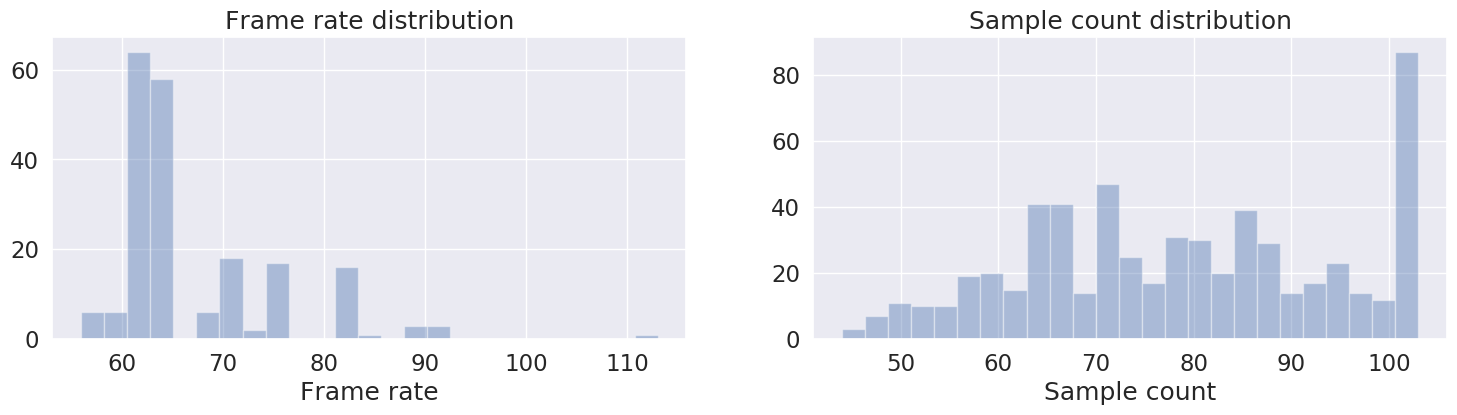
\includegraphics[width=\textwidth]{data-exp/fr_sample_dist.png}
    %% Creator: Matplotlib, PGF backend
%%
%% To include the figure in your LaTeX document, write
%%   \input{<filename>.pgf}
%%
%% Make sure the required packages are loaded in your preamble
%%   \usepackage{pgf}
%%
%% Figures using additional raster images can only be included by \input if
%% they are in the same directory as the main LaTeX file. For loading figures
%% from other directories you can use the `import` package
%%   \usepackage{import}
%% and then include the figures with
%%   \import{<path to file>}{<filename>.pgf}
%%
%% Matplotlib used the following preamble
%%
\begingroup%
\makeatletter%
\begin{pgfpicture}%
\pgfpathrectangle{\pgfpointorigin}{\pgfqpoint{5.532637in}{2.422869in}}%
\pgfusepath{use as bounding box, clip}%
\begin{pgfscope}%
\pgfsetbuttcap%
\pgfsetmiterjoin%
\definecolor{currentfill}{rgb}{1.000000,1.000000,1.000000}%
\pgfsetfillcolor{currentfill}%
\pgfsetlinewidth{0.000000pt}%
\definecolor{currentstroke}{rgb}{1.000000,1.000000,1.000000}%
\pgfsetstrokecolor{currentstroke}%
\pgfsetdash{}{0pt}%
\pgfpathmoveto{\pgfqpoint{0.000000in}{0.000000in}}%
\pgfpathlineto{\pgfqpoint{5.532637in}{0.000000in}}%
\pgfpathlineto{\pgfqpoint{5.532637in}{2.422869in}}%
\pgfpathlineto{\pgfqpoint{0.000000in}{2.422869in}}%
\pgfpathclose%
\pgfusepath{fill}%
\end{pgfscope}%
\begin{pgfscope}%
\pgfsetbuttcap%
\pgfsetmiterjoin%
\definecolor{currentfill}{rgb}{0.917647,0.917647,0.949020}%
\pgfsetfillcolor{currentfill}%
\pgfsetlinewidth{0.000000pt}%
\definecolor{currentstroke}{rgb}{0.000000,0.000000,0.000000}%
\pgfsetstrokecolor{currentstroke}%
\pgfsetstrokeopacity{0.000000}%
\pgfsetdash{}{0pt}%
\pgfpathmoveto{\pgfqpoint{0.395137in}{0.583795in}}%
\pgfpathlineto{\pgfqpoint{2.684910in}{0.583795in}}%
\pgfpathlineto{\pgfqpoint{2.684910in}{2.123795in}}%
\pgfpathlineto{\pgfqpoint{0.395137in}{2.123795in}}%
\pgfpathclose%
\pgfusepath{fill}%
\end{pgfscope}%
\begin{pgfscope}%
\pgfpathrectangle{\pgfqpoint{0.395137in}{0.583795in}}{\pgfqpoint{2.289773in}{1.540000in}}%
\pgfusepath{clip}%
\pgfsetroundcap%
\pgfsetroundjoin%
\pgfsetlinewidth{1.003750pt}%
\definecolor{currentstroke}{rgb}{1.000000,1.000000,1.000000}%
\pgfsetstrokecolor{currentstroke}%
\pgfsetdash{}{0pt}%
\pgfpathmoveto{\pgfqpoint{0.645296in}{0.583795in}}%
\pgfpathlineto{\pgfqpoint{0.645296in}{2.123795in}}%
\pgfusepath{stroke}%
\end{pgfscope}%
\begin{pgfscope}%
\definecolor{textcolor}{rgb}{0.150000,0.150000,0.150000}%
\pgfsetstrokecolor{textcolor}%
\pgfsetfillcolor{textcolor}%
\pgftext[x=0.645296in,y=0.451851in,,top]{\color{textcolor}\sffamily\fontsize{12.000000}{14.400000}\selectfont \(\displaystyle 60\)}%
\end{pgfscope}%
\begin{pgfscope}%
\pgfpathrectangle{\pgfqpoint{0.395137in}{0.583795in}}{\pgfqpoint{2.289773in}{1.540000in}}%
\pgfusepath{clip}%
\pgfsetroundcap%
\pgfsetroundjoin%
\pgfsetlinewidth{1.003750pt}%
\definecolor{currentstroke}{rgb}{1.000000,1.000000,1.000000}%
\pgfsetstrokecolor{currentstroke}%
\pgfsetdash{}{0pt}%
\pgfpathmoveto{\pgfqpoint{1.375686in}{0.583795in}}%
\pgfpathlineto{\pgfqpoint{1.375686in}{2.123795in}}%
\pgfusepath{stroke}%
\end{pgfscope}%
\begin{pgfscope}%
\definecolor{textcolor}{rgb}{0.150000,0.150000,0.150000}%
\pgfsetstrokecolor{textcolor}%
\pgfsetfillcolor{textcolor}%
\pgftext[x=1.375686in,y=0.451851in,,top]{\color{textcolor}\sffamily\fontsize{12.000000}{14.400000}\selectfont \(\displaystyle 80\)}%
\end{pgfscope}%
\begin{pgfscope}%
\pgfpathrectangle{\pgfqpoint{0.395137in}{0.583795in}}{\pgfqpoint{2.289773in}{1.540000in}}%
\pgfusepath{clip}%
\pgfsetroundcap%
\pgfsetroundjoin%
\pgfsetlinewidth{1.003750pt}%
\definecolor{currentstroke}{rgb}{1.000000,1.000000,1.000000}%
\pgfsetstrokecolor{currentstroke}%
\pgfsetdash{}{0pt}%
\pgfpathmoveto{\pgfqpoint{2.106076in}{0.583795in}}%
\pgfpathlineto{\pgfqpoint{2.106076in}{2.123795in}}%
\pgfusepath{stroke}%
\end{pgfscope}%
\begin{pgfscope}%
\definecolor{textcolor}{rgb}{0.150000,0.150000,0.150000}%
\pgfsetstrokecolor{textcolor}%
\pgfsetfillcolor{textcolor}%
\pgftext[x=2.106076in,y=0.451851in,,top]{\color{textcolor}\sffamily\fontsize{12.000000}{14.400000}\selectfont \(\displaystyle 100\)}%
\end{pgfscope}%
\begin{pgfscope}%
\definecolor{textcolor}{rgb}{0.150000,0.150000,0.150000}%
\pgfsetstrokecolor{textcolor}%
\pgfsetfillcolor{textcolor}%
\pgftext[x=1.540024in,y=0.248148in,,top]{\color{textcolor}\sffamily\fontsize{12.000000}{14.400000}\selectfont Frame rate}%
\end{pgfscope}%
\begin{pgfscope}%
\pgfpathrectangle{\pgfqpoint{0.395137in}{0.583795in}}{\pgfqpoint{2.289773in}{1.540000in}}%
\pgfusepath{clip}%
\pgfsetroundcap%
\pgfsetroundjoin%
\pgfsetlinewidth{1.003750pt}%
\definecolor{currentstroke}{rgb}{1.000000,1.000000,1.000000}%
\pgfsetstrokecolor{currentstroke}%
\pgfsetdash{}{0pt}%
\pgfpathmoveto{\pgfqpoint{0.395137in}{0.583795in}}%
\pgfpathlineto{\pgfqpoint{2.684910in}{0.583795in}}%
\pgfusepath{stroke}%
\end{pgfscope}%
\begin{pgfscope}%
\definecolor{textcolor}{rgb}{0.150000,0.150000,0.150000}%
\pgfsetstrokecolor{textcolor}%
\pgfsetfillcolor{textcolor}%
\pgftext[x=0.181596in,y=0.525925in,left,base]{\color{textcolor}\sffamily\fontsize{12.000000}{14.400000}\selectfont \(\displaystyle 0\)}%
\end{pgfscope}%
\begin{pgfscope}%
\pgfpathrectangle{\pgfqpoint{0.395137in}{0.583795in}}{\pgfqpoint{2.289773in}{1.540000in}}%
\pgfusepath{clip}%
\pgfsetroundcap%
\pgfsetroundjoin%
\pgfsetlinewidth{1.003750pt}%
\definecolor{currentstroke}{rgb}{1.000000,1.000000,1.000000}%
\pgfsetstrokecolor{currentstroke}%
\pgfsetdash{}{0pt}%
\pgfpathmoveto{\pgfqpoint{0.395137in}{1.042128in}}%
\pgfpathlineto{\pgfqpoint{2.684910in}{1.042128in}}%
\pgfusepath{stroke}%
\end{pgfscope}%
\begin{pgfscope}%
\definecolor{textcolor}{rgb}{0.150000,0.150000,0.150000}%
\pgfsetstrokecolor{textcolor}%
\pgfsetfillcolor{textcolor}%
\pgftext[x=0.100000in,y=0.984258in,left,base]{\color{textcolor}\sffamily\fontsize{12.000000}{14.400000}\selectfont \(\displaystyle 20\)}%
\end{pgfscope}%
\begin{pgfscope}%
\pgfpathrectangle{\pgfqpoint{0.395137in}{0.583795in}}{\pgfqpoint{2.289773in}{1.540000in}}%
\pgfusepath{clip}%
\pgfsetroundcap%
\pgfsetroundjoin%
\pgfsetlinewidth{1.003750pt}%
\definecolor{currentstroke}{rgb}{1.000000,1.000000,1.000000}%
\pgfsetstrokecolor{currentstroke}%
\pgfsetdash{}{0pt}%
\pgfpathmoveto{\pgfqpoint{0.395137in}{1.500462in}}%
\pgfpathlineto{\pgfqpoint{2.684910in}{1.500462in}}%
\pgfusepath{stroke}%
\end{pgfscope}%
\begin{pgfscope}%
\definecolor{textcolor}{rgb}{0.150000,0.150000,0.150000}%
\pgfsetstrokecolor{textcolor}%
\pgfsetfillcolor{textcolor}%
\pgftext[x=0.100000in,y=1.442591in,left,base]{\color{textcolor}\sffamily\fontsize{12.000000}{14.400000}\selectfont \(\displaystyle 40\)}%
\end{pgfscope}%
\begin{pgfscope}%
\pgfpathrectangle{\pgfqpoint{0.395137in}{0.583795in}}{\pgfqpoint{2.289773in}{1.540000in}}%
\pgfusepath{clip}%
\pgfsetroundcap%
\pgfsetroundjoin%
\pgfsetlinewidth{1.003750pt}%
\definecolor{currentstroke}{rgb}{1.000000,1.000000,1.000000}%
\pgfsetstrokecolor{currentstroke}%
\pgfsetdash{}{0pt}%
\pgfpathmoveto{\pgfqpoint{0.395137in}{1.958795in}}%
\pgfpathlineto{\pgfqpoint{2.684910in}{1.958795in}}%
\pgfusepath{stroke}%
\end{pgfscope}%
\begin{pgfscope}%
\definecolor{textcolor}{rgb}{0.150000,0.150000,0.150000}%
\pgfsetstrokecolor{textcolor}%
\pgfsetfillcolor{textcolor}%
\pgftext[x=0.100000in,y=1.900925in,left,base]{\color{textcolor}\sffamily\fontsize{12.000000}{14.400000}\selectfont \(\displaystyle 60\)}%
\end{pgfscope}%
\begin{pgfscope}%
\pgfpathrectangle{\pgfqpoint{0.395137in}{0.583795in}}{\pgfqpoint{2.289773in}{1.540000in}}%
\pgfusepath{clip}%
\pgfsetbuttcap%
\pgfsetmiterjoin%
\definecolor{currentfill}{rgb}{0.298039,0.447059,0.690196}%
\pgfsetfillcolor{currentfill}%
\pgfsetfillopacity{0.400000}%
\pgfsetlinewidth{1.003750pt}%
\definecolor{currentstroke}{rgb}{1.000000,1.000000,1.000000}%
\pgfsetstrokecolor{currentstroke}%
\pgfsetstrokeopacity{0.400000}%
\pgfsetdash{}{0pt}%
\pgfpathmoveto{\pgfqpoint{0.499218in}{0.583795in}}%
\pgfpathlineto{\pgfqpoint{0.582482in}{0.583795in}}%
\pgfpathlineto{\pgfqpoint{0.582482in}{0.721295in}}%
\pgfpathlineto{\pgfqpoint{0.499218in}{0.721295in}}%
\pgfpathclose%
\pgfusepath{stroke,fill}%
\end{pgfscope}%
\begin{pgfscope}%
\pgfpathrectangle{\pgfqpoint{0.395137in}{0.583795in}}{\pgfqpoint{2.289773in}{1.540000in}}%
\pgfusepath{clip}%
\pgfsetbuttcap%
\pgfsetmiterjoin%
\definecolor{currentfill}{rgb}{0.298039,0.447059,0.690196}%
\pgfsetfillcolor{currentfill}%
\pgfsetfillopacity{0.400000}%
\pgfsetlinewidth{1.003750pt}%
\definecolor{currentstroke}{rgb}{1.000000,1.000000,1.000000}%
\pgfsetstrokecolor{currentstroke}%
\pgfsetstrokeopacity{0.400000}%
\pgfsetdash{}{0pt}%
\pgfpathmoveto{\pgfqpoint{0.582482in}{0.583795in}}%
\pgfpathlineto{\pgfqpoint{0.665747in}{0.583795in}}%
\pgfpathlineto{\pgfqpoint{0.665747in}{0.721295in}}%
\pgfpathlineto{\pgfqpoint{0.582482in}{0.721295in}}%
\pgfpathclose%
\pgfusepath{stroke,fill}%
\end{pgfscope}%
\begin{pgfscope}%
\pgfpathrectangle{\pgfqpoint{0.395137in}{0.583795in}}{\pgfqpoint{2.289773in}{1.540000in}}%
\pgfusepath{clip}%
\pgfsetbuttcap%
\pgfsetmiterjoin%
\definecolor{currentfill}{rgb}{0.298039,0.447059,0.690196}%
\pgfsetfillcolor{currentfill}%
\pgfsetfillopacity{0.400000}%
\pgfsetlinewidth{1.003750pt}%
\definecolor{currentstroke}{rgb}{1.000000,1.000000,1.000000}%
\pgfsetstrokecolor{currentstroke}%
\pgfsetstrokeopacity{0.400000}%
\pgfsetdash{}{0pt}%
\pgfpathmoveto{\pgfqpoint{0.665747in}{0.583795in}}%
\pgfpathlineto{\pgfqpoint{0.749011in}{0.583795in}}%
\pgfpathlineto{\pgfqpoint{0.749011in}{2.050462in}}%
\pgfpathlineto{\pgfqpoint{0.665747in}{2.050462in}}%
\pgfpathclose%
\pgfusepath{stroke,fill}%
\end{pgfscope}%
\begin{pgfscope}%
\pgfpathrectangle{\pgfqpoint{0.395137in}{0.583795in}}{\pgfqpoint{2.289773in}{1.540000in}}%
\pgfusepath{clip}%
\pgfsetbuttcap%
\pgfsetmiterjoin%
\definecolor{currentfill}{rgb}{0.298039,0.447059,0.690196}%
\pgfsetfillcolor{currentfill}%
\pgfsetfillopacity{0.400000}%
\pgfsetlinewidth{1.003750pt}%
\definecolor{currentstroke}{rgb}{1.000000,1.000000,1.000000}%
\pgfsetstrokecolor{currentstroke}%
\pgfsetstrokeopacity{0.400000}%
\pgfsetdash{}{0pt}%
\pgfpathmoveto{\pgfqpoint{0.749011in}{0.583795in}}%
\pgfpathlineto{\pgfqpoint{0.832276in}{0.583795in}}%
\pgfpathlineto{\pgfqpoint{0.832276in}{1.912962in}}%
\pgfpathlineto{\pgfqpoint{0.749011in}{1.912962in}}%
\pgfpathclose%
\pgfusepath{stroke,fill}%
\end{pgfscope}%
\begin{pgfscope}%
\pgfpathrectangle{\pgfqpoint{0.395137in}{0.583795in}}{\pgfqpoint{2.289773in}{1.540000in}}%
\pgfusepath{clip}%
\pgfsetbuttcap%
\pgfsetmiterjoin%
\definecolor{currentfill}{rgb}{0.298039,0.447059,0.690196}%
\pgfsetfillcolor{currentfill}%
\pgfsetfillopacity{0.400000}%
\pgfsetlinewidth{1.003750pt}%
\definecolor{currentstroke}{rgb}{1.000000,1.000000,1.000000}%
\pgfsetstrokecolor{currentstroke}%
\pgfsetstrokeopacity{0.400000}%
\pgfsetdash{}{0pt}%
\pgfpathmoveto{\pgfqpoint{0.832276in}{0.583795in}}%
\pgfpathlineto{\pgfqpoint{0.915540in}{0.583795in}}%
\pgfpathlineto{\pgfqpoint{0.915540in}{0.583795in}}%
\pgfpathlineto{\pgfqpoint{0.832276in}{0.583795in}}%
\pgfpathclose%
\pgfusepath{stroke,fill}%
\end{pgfscope}%
\begin{pgfscope}%
\pgfpathrectangle{\pgfqpoint{0.395137in}{0.583795in}}{\pgfqpoint{2.289773in}{1.540000in}}%
\pgfusepath{clip}%
\pgfsetbuttcap%
\pgfsetmiterjoin%
\definecolor{currentfill}{rgb}{0.298039,0.447059,0.690196}%
\pgfsetfillcolor{currentfill}%
\pgfsetfillopacity{0.400000}%
\pgfsetlinewidth{1.003750pt}%
\definecolor{currentstroke}{rgb}{1.000000,1.000000,1.000000}%
\pgfsetstrokecolor{currentstroke}%
\pgfsetstrokeopacity{0.400000}%
\pgfsetdash{}{0pt}%
\pgfpathmoveto{\pgfqpoint{0.915540in}{0.583795in}}%
\pgfpathlineto{\pgfqpoint{0.998805in}{0.583795in}}%
\pgfpathlineto{\pgfqpoint{0.998805in}{0.721295in}}%
\pgfpathlineto{\pgfqpoint{0.915540in}{0.721295in}}%
\pgfpathclose%
\pgfusepath{stroke,fill}%
\end{pgfscope}%
\begin{pgfscope}%
\pgfpathrectangle{\pgfqpoint{0.395137in}{0.583795in}}{\pgfqpoint{2.289773in}{1.540000in}}%
\pgfusepath{clip}%
\pgfsetbuttcap%
\pgfsetmiterjoin%
\definecolor{currentfill}{rgb}{0.298039,0.447059,0.690196}%
\pgfsetfillcolor{currentfill}%
\pgfsetfillopacity{0.400000}%
\pgfsetlinewidth{1.003750pt}%
\definecolor{currentstroke}{rgb}{1.000000,1.000000,1.000000}%
\pgfsetstrokecolor{currentstroke}%
\pgfsetstrokeopacity{0.400000}%
\pgfsetdash{}{0pt}%
\pgfpathmoveto{\pgfqpoint{0.998805in}{0.583795in}}%
\pgfpathlineto{\pgfqpoint{1.082069in}{0.583795in}}%
\pgfpathlineto{\pgfqpoint{1.082069in}{0.996295in}}%
\pgfpathlineto{\pgfqpoint{0.998805in}{0.996295in}}%
\pgfpathclose%
\pgfusepath{stroke,fill}%
\end{pgfscope}%
\begin{pgfscope}%
\pgfpathrectangle{\pgfqpoint{0.395137in}{0.583795in}}{\pgfqpoint{2.289773in}{1.540000in}}%
\pgfusepath{clip}%
\pgfsetbuttcap%
\pgfsetmiterjoin%
\definecolor{currentfill}{rgb}{0.298039,0.447059,0.690196}%
\pgfsetfillcolor{currentfill}%
\pgfsetfillopacity{0.400000}%
\pgfsetlinewidth{1.003750pt}%
\definecolor{currentstroke}{rgb}{1.000000,1.000000,1.000000}%
\pgfsetstrokecolor{currentstroke}%
\pgfsetstrokeopacity{0.400000}%
\pgfsetdash{}{0pt}%
\pgfpathmoveto{\pgfqpoint{1.082069in}{0.583795in}}%
\pgfpathlineto{\pgfqpoint{1.165334in}{0.583795in}}%
\pgfpathlineto{\pgfqpoint{1.165334in}{0.629628in}}%
\pgfpathlineto{\pgfqpoint{1.082069in}{0.629628in}}%
\pgfpathclose%
\pgfusepath{stroke,fill}%
\end{pgfscope}%
\begin{pgfscope}%
\pgfpathrectangle{\pgfqpoint{0.395137in}{0.583795in}}{\pgfqpoint{2.289773in}{1.540000in}}%
\pgfusepath{clip}%
\pgfsetbuttcap%
\pgfsetmiterjoin%
\definecolor{currentfill}{rgb}{0.298039,0.447059,0.690196}%
\pgfsetfillcolor{currentfill}%
\pgfsetfillopacity{0.400000}%
\pgfsetlinewidth{1.003750pt}%
\definecolor{currentstroke}{rgb}{1.000000,1.000000,1.000000}%
\pgfsetstrokecolor{currentstroke}%
\pgfsetstrokeopacity{0.400000}%
\pgfsetdash{}{0pt}%
\pgfpathmoveto{\pgfqpoint{1.165334in}{0.583795in}}%
\pgfpathlineto{\pgfqpoint{1.248598in}{0.583795in}}%
\pgfpathlineto{\pgfqpoint{1.248598in}{0.973378in}}%
\pgfpathlineto{\pgfqpoint{1.165334in}{0.973378in}}%
\pgfpathclose%
\pgfusepath{stroke,fill}%
\end{pgfscope}%
\begin{pgfscope}%
\pgfpathrectangle{\pgfqpoint{0.395137in}{0.583795in}}{\pgfqpoint{2.289773in}{1.540000in}}%
\pgfusepath{clip}%
\pgfsetbuttcap%
\pgfsetmiterjoin%
\definecolor{currentfill}{rgb}{0.298039,0.447059,0.690196}%
\pgfsetfillcolor{currentfill}%
\pgfsetfillopacity{0.400000}%
\pgfsetlinewidth{1.003750pt}%
\definecolor{currentstroke}{rgb}{1.000000,1.000000,1.000000}%
\pgfsetstrokecolor{currentstroke}%
\pgfsetstrokeopacity{0.400000}%
\pgfsetdash{}{0pt}%
\pgfpathmoveto{\pgfqpoint{1.248598in}{0.583795in}}%
\pgfpathlineto{\pgfqpoint{1.331862in}{0.583795in}}%
\pgfpathlineto{\pgfqpoint{1.331862in}{0.583795in}}%
\pgfpathlineto{\pgfqpoint{1.248598in}{0.583795in}}%
\pgfpathclose%
\pgfusepath{stroke,fill}%
\end{pgfscope}%
\begin{pgfscope}%
\pgfpathrectangle{\pgfqpoint{0.395137in}{0.583795in}}{\pgfqpoint{2.289773in}{1.540000in}}%
\pgfusepath{clip}%
\pgfsetbuttcap%
\pgfsetmiterjoin%
\definecolor{currentfill}{rgb}{0.298039,0.447059,0.690196}%
\pgfsetfillcolor{currentfill}%
\pgfsetfillopacity{0.400000}%
\pgfsetlinewidth{1.003750pt}%
\definecolor{currentstroke}{rgb}{1.000000,1.000000,1.000000}%
\pgfsetstrokecolor{currentstroke}%
\pgfsetstrokeopacity{0.400000}%
\pgfsetdash{}{0pt}%
\pgfpathmoveto{\pgfqpoint{1.331862in}{0.583795in}}%
\pgfpathlineto{\pgfqpoint{1.415127in}{0.583795in}}%
\pgfpathlineto{\pgfqpoint{1.415127in}{0.583795in}}%
\pgfpathlineto{\pgfqpoint{1.331862in}{0.583795in}}%
\pgfpathclose%
\pgfusepath{stroke,fill}%
\end{pgfscope}%
\begin{pgfscope}%
\pgfpathrectangle{\pgfqpoint{0.395137in}{0.583795in}}{\pgfqpoint{2.289773in}{1.540000in}}%
\pgfusepath{clip}%
\pgfsetbuttcap%
\pgfsetmiterjoin%
\definecolor{currentfill}{rgb}{0.298039,0.447059,0.690196}%
\pgfsetfillcolor{currentfill}%
\pgfsetfillopacity{0.400000}%
\pgfsetlinewidth{1.003750pt}%
\definecolor{currentstroke}{rgb}{1.000000,1.000000,1.000000}%
\pgfsetstrokecolor{currentstroke}%
\pgfsetstrokeopacity{0.400000}%
\pgfsetdash{}{0pt}%
\pgfpathmoveto{\pgfqpoint{1.415127in}{0.583795in}}%
\pgfpathlineto{\pgfqpoint{1.498391in}{0.583795in}}%
\pgfpathlineto{\pgfqpoint{1.498391in}{0.950462in}}%
\pgfpathlineto{\pgfqpoint{1.415127in}{0.950462in}}%
\pgfpathclose%
\pgfusepath{stroke,fill}%
\end{pgfscope}%
\begin{pgfscope}%
\pgfpathrectangle{\pgfqpoint{0.395137in}{0.583795in}}{\pgfqpoint{2.289773in}{1.540000in}}%
\pgfusepath{clip}%
\pgfsetbuttcap%
\pgfsetmiterjoin%
\definecolor{currentfill}{rgb}{0.298039,0.447059,0.690196}%
\pgfsetfillcolor{currentfill}%
\pgfsetfillopacity{0.400000}%
\pgfsetlinewidth{1.003750pt}%
\definecolor{currentstroke}{rgb}{1.000000,1.000000,1.000000}%
\pgfsetstrokecolor{currentstroke}%
\pgfsetstrokeopacity{0.400000}%
\pgfsetdash{}{0pt}%
\pgfpathmoveto{\pgfqpoint{1.498391in}{0.583795in}}%
\pgfpathlineto{\pgfqpoint{1.581656in}{0.583795in}}%
\pgfpathlineto{\pgfqpoint{1.581656in}{0.606712in}}%
\pgfpathlineto{\pgfqpoint{1.498391in}{0.606712in}}%
\pgfpathclose%
\pgfusepath{stroke,fill}%
\end{pgfscope}%
\begin{pgfscope}%
\pgfpathrectangle{\pgfqpoint{0.395137in}{0.583795in}}{\pgfqpoint{2.289773in}{1.540000in}}%
\pgfusepath{clip}%
\pgfsetbuttcap%
\pgfsetmiterjoin%
\definecolor{currentfill}{rgb}{0.298039,0.447059,0.690196}%
\pgfsetfillcolor{currentfill}%
\pgfsetfillopacity{0.400000}%
\pgfsetlinewidth{1.003750pt}%
\definecolor{currentstroke}{rgb}{1.000000,1.000000,1.000000}%
\pgfsetstrokecolor{currentstroke}%
\pgfsetstrokeopacity{0.400000}%
\pgfsetdash{}{0pt}%
\pgfpathmoveto{\pgfqpoint{1.581656in}{0.583795in}}%
\pgfpathlineto{\pgfqpoint{1.664920in}{0.583795in}}%
\pgfpathlineto{\pgfqpoint{1.664920in}{0.583795in}}%
\pgfpathlineto{\pgfqpoint{1.581656in}{0.583795in}}%
\pgfpathclose%
\pgfusepath{stroke,fill}%
\end{pgfscope}%
\begin{pgfscope}%
\pgfpathrectangle{\pgfqpoint{0.395137in}{0.583795in}}{\pgfqpoint{2.289773in}{1.540000in}}%
\pgfusepath{clip}%
\pgfsetbuttcap%
\pgfsetmiterjoin%
\definecolor{currentfill}{rgb}{0.298039,0.447059,0.690196}%
\pgfsetfillcolor{currentfill}%
\pgfsetfillopacity{0.400000}%
\pgfsetlinewidth{1.003750pt}%
\definecolor{currentstroke}{rgb}{1.000000,1.000000,1.000000}%
\pgfsetstrokecolor{currentstroke}%
\pgfsetstrokeopacity{0.400000}%
\pgfsetdash{}{0pt}%
\pgfpathmoveto{\pgfqpoint{1.664920in}{0.583795in}}%
\pgfpathlineto{\pgfqpoint{1.748185in}{0.583795in}}%
\pgfpathlineto{\pgfqpoint{1.748185in}{0.652545in}}%
\pgfpathlineto{\pgfqpoint{1.664920in}{0.652545in}}%
\pgfpathclose%
\pgfusepath{stroke,fill}%
\end{pgfscope}%
\begin{pgfscope}%
\pgfpathrectangle{\pgfqpoint{0.395137in}{0.583795in}}{\pgfqpoint{2.289773in}{1.540000in}}%
\pgfusepath{clip}%
\pgfsetbuttcap%
\pgfsetmiterjoin%
\definecolor{currentfill}{rgb}{0.298039,0.447059,0.690196}%
\pgfsetfillcolor{currentfill}%
\pgfsetfillopacity{0.400000}%
\pgfsetlinewidth{1.003750pt}%
\definecolor{currentstroke}{rgb}{1.000000,1.000000,1.000000}%
\pgfsetstrokecolor{currentstroke}%
\pgfsetstrokeopacity{0.400000}%
\pgfsetdash{}{0pt}%
\pgfpathmoveto{\pgfqpoint{1.748185in}{0.583795in}}%
\pgfpathlineto{\pgfqpoint{1.831449in}{0.583795in}}%
\pgfpathlineto{\pgfqpoint{1.831449in}{0.652545in}}%
\pgfpathlineto{\pgfqpoint{1.748185in}{0.652545in}}%
\pgfpathclose%
\pgfusepath{stroke,fill}%
\end{pgfscope}%
\begin{pgfscope}%
\pgfpathrectangle{\pgfqpoint{0.395137in}{0.583795in}}{\pgfqpoint{2.289773in}{1.540000in}}%
\pgfusepath{clip}%
\pgfsetbuttcap%
\pgfsetmiterjoin%
\definecolor{currentfill}{rgb}{0.298039,0.447059,0.690196}%
\pgfsetfillcolor{currentfill}%
\pgfsetfillopacity{0.400000}%
\pgfsetlinewidth{1.003750pt}%
\definecolor{currentstroke}{rgb}{1.000000,1.000000,1.000000}%
\pgfsetstrokecolor{currentstroke}%
\pgfsetstrokeopacity{0.400000}%
\pgfsetdash{}{0pt}%
\pgfpathmoveto{\pgfqpoint{1.831449in}{0.583795in}}%
\pgfpathlineto{\pgfqpoint{1.914714in}{0.583795in}}%
\pgfpathlineto{\pgfqpoint{1.914714in}{0.583795in}}%
\pgfpathlineto{\pgfqpoint{1.831449in}{0.583795in}}%
\pgfpathclose%
\pgfusepath{stroke,fill}%
\end{pgfscope}%
\begin{pgfscope}%
\pgfpathrectangle{\pgfqpoint{0.395137in}{0.583795in}}{\pgfqpoint{2.289773in}{1.540000in}}%
\pgfusepath{clip}%
\pgfsetbuttcap%
\pgfsetmiterjoin%
\definecolor{currentfill}{rgb}{0.298039,0.447059,0.690196}%
\pgfsetfillcolor{currentfill}%
\pgfsetfillopacity{0.400000}%
\pgfsetlinewidth{1.003750pt}%
\definecolor{currentstroke}{rgb}{1.000000,1.000000,1.000000}%
\pgfsetstrokecolor{currentstroke}%
\pgfsetstrokeopacity{0.400000}%
\pgfsetdash{}{0pt}%
\pgfpathmoveto{\pgfqpoint{1.914714in}{0.583795in}}%
\pgfpathlineto{\pgfqpoint{1.997978in}{0.583795in}}%
\pgfpathlineto{\pgfqpoint{1.997978in}{0.583795in}}%
\pgfpathlineto{\pgfqpoint{1.914714in}{0.583795in}}%
\pgfpathclose%
\pgfusepath{stroke,fill}%
\end{pgfscope}%
\begin{pgfscope}%
\pgfpathrectangle{\pgfqpoint{0.395137in}{0.583795in}}{\pgfqpoint{2.289773in}{1.540000in}}%
\pgfusepath{clip}%
\pgfsetbuttcap%
\pgfsetmiterjoin%
\definecolor{currentfill}{rgb}{0.298039,0.447059,0.690196}%
\pgfsetfillcolor{currentfill}%
\pgfsetfillopacity{0.400000}%
\pgfsetlinewidth{1.003750pt}%
\definecolor{currentstroke}{rgb}{1.000000,1.000000,1.000000}%
\pgfsetstrokecolor{currentstroke}%
\pgfsetstrokeopacity{0.400000}%
\pgfsetdash{}{0pt}%
\pgfpathmoveto{\pgfqpoint{1.997978in}{0.583795in}}%
\pgfpathlineto{\pgfqpoint{2.081243in}{0.583795in}}%
\pgfpathlineto{\pgfqpoint{2.081243in}{0.583795in}}%
\pgfpathlineto{\pgfqpoint{1.997978in}{0.583795in}}%
\pgfpathclose%
\pgfusepath{stroke,fill}%
\end{pgfscope}%
\begin{pgfscope}%
\pgfpathrectangle{\pgfqpoint{0.395137in}{0.583795in}}{\pgfqpoint{2.289773in}{1.540000in}}%
\pgfusepath{clip}%
\pgfsetbuttcap%
\pgfsetmiterjoin%
\definecolor{currentfill}{rgb}{0.298039,0.447059,0.690196}%
\pgfsetfillcolor{currentfill}%
\pgfsetfillopacity{0.400000}%
\pgfsetlinewidth{1.003750pt}%
\definecolor{currentstroke}{rgb}{1.000000,1.000000,1.000000}%
\pgfsetstrokecolor{currentstroke}%
\pgfsetstrokeopacity{0.400000}%
\pgfsetdash{}{0pt}%
\pgfpathmoveto{\pgfqpoint{2.081243in}{0.583795in}}%
\pgfpathlineto{\pgfqpoint{2.164507in}{0.583795in}}%
\pgfpathlineto{\pgfqpoint{2.164507in}{0.583795in}}%
\pgfpathlineto{\pgfqpoint{2.081243in}{0.583795in}}%
\pgfpathclose%
\pgfusepath{stroke,fill}%
\end{pgfscope}%
\begin{pgfscope}%
\pgfpathrectangle{\pgfqpoint{0.395137in}{0.583795in}}{\pgfqpoint{2.289773in}{1.540000in}}%
\pgfusepath{clip}%
\pgfsetbuttcap%
\pgfsetmiterjoin%
\definecolor{currentfill}{rgb}{0.298039,0.447059,0.690196}%
\pgfsetfillcolor{currentfill}%
\pgfsetfillopacity{0.400000}%
\pgfsetlinewidth{1.003750pt}%
\definecolor{currentstroke}{rgb}{1.000000,1.000000,1.000000}%
\pgfsetstrokecolor{currentstroke}%
\pgfsetstrokeopacity{0.400000}%
\pgfsetdash{}{0pt}%
\pgfpathmoveto{\pgfqpoint{2.164507in}{0.583795in}}%
\pgfpathlineto{\pgfqpoint{2.247772in}{0.583795in}}%
\pgfpathlineto{\pgfqpoint{2.247772in}{0.583795in}}%
\pgfpathlineto{\pgfqpoint{2.164507in}{0.583795in}}%
\pgfpathclose%
\pgfusepath{stroke,fill}%
\end{pgfscope}%
\begin{pgfscope}%
\pgfpathrectangle{\pgfqpoint{0.395137in}{0.583795in}}{\pgfqpoint{2.289773in}{1.540000in}}%
\pgfusepath{clip}%
\pgfsetbuttcap%
\pgfsetmiterjoin%
\definecolor{currentfill}{rgb}{0.298039,0.447059,0.690196}%
\pgfsetfillcolor{currentfill}%
\pgfsetfillopacity{0.400000}%
\pgfsetlinewidth{1.003750pt}%
\definecolor{currentstroke}{rgb}{1.000000,1.000000,1.000000}%
\pgfsetstrokecolor{currentstroke}%
\pgfsetstrokeopacity{0.400000}%
\pgfsetdash{}{0pt}%
\pgfpathmoveto{\pgfqpoint{2.247772in}{0.583795in}}%
\pgfpathlineto{\pgfqpoint{2.331036in}{0.583795in}}%
\pgfpathlineto{\pgfqpoint{2.331036in}{0.583795in}}%
\pgfpathlineto{\pgfqpoint{2.247772in}{0.583795in}}%
\pgfpathclose%
\pgfusepath{stroke,fill}%
\end{pgfscope}%
\begin{pgfscope}%
\pgfpathrectangle{\pgfqpoint{0.395137in}{0.583795in}}{\pgfqpoint{2.289773in}{1.540000in}}%
\pgfusepath{clip}%
\pgfsetbuttcap%
\pgfsetmiterjoin%
\definecolor{currentfill}{rgb}{0.298039,0.447059,0.690196}%
\pgfsetfillcolor{currentfill}%
\pgfsetfillopacity{0.400000}%
\pgfsetlinewidth{1.003750pt}%
\definecolor{currentstroke}{rgb}{1.000000,1.000000,1.000000}%
\pgfsetstrokecolor{currentstroke}%
\pgfsetstrokeopacity{0.400000}%
\pgfsetdash{}{0pt}%
\pgfpathmoveto{\pgfqpoint{2.331036in}{0.583795in}}%
\pgfpathlineto{\pgfqpoint{2.414300in}{0.583795in}}%
\pgfpathlineto{\pgfqpoint{2.414300in}{0.583795in}}%
\pgfpathlineto{\pgfqpoint{2.331036in}{0.583795in}}%
\pgfpathclose%
\pgfusepath{stroke,fill}%
\end{pgfscope}%
\begin{pgfscope}%
\pgfpathrectangle{\pgfqpoint{0.395137in}{0.583795in}}{\pgfqpoint{2.289773in}{1.540000in}}%
\pgfusepath{clip}%
\pgfsetbuttcap%
\pgfsetmiterjoin%
\definecolor{currentfill}{rgb}{0.298039,0.447059,0.690196}%
\pgfsetfillcolor{currentfill}%
\pgfsetfillopacity{0.400000}%
\pgfsetlinewidth{1.003750pt}%
\definecolor{currentstroke}{rgb}{1.000000,1.000000,1.000000}%
\pgfsetstrokecolor{currentstroke}%
\pgfsetstrokeopacity{0.400000}%
\pgfsetdash{}{0pt}%
\pgfpathmoveto{\pgfqpoint{2.414300in}{0.583795in}}%
\pgfpathlineto{\pgfqpoint{2.497565in}{0.583795in}}%
\pgfpathlineto{\pgfqpoint{2.497565in}{0.583795in}}%
\pgfpathlineto{\pgfqpoint{2.414300in}{0.583795in}}%
\pgfpathclose%
\pgfusepath{stroke,fill}%
\end{pgfscope}%
\begin{pgfscope}%
\pgfpathrectangle{\pgfqpoint{0.395137in}{0.583795in}}{\pgfqpoint{2.289773in}{1.540000in}}%
\pgfusepath{clip}%
\pgfsetbuttcap%
\pgfsetmiterjoin%
\definecolor{currentfill}{rgb}{0.298039,0.447059,0.690196}%
\pgfsetfillcolor{currentfill}%
\pgfsetfillopacity{0.400000}%
\pgfsetlinewidth{1.003750pt}%
\definecolor{currentstroke}{rgb}{1.000000,1.000000,1.000000}%
\pgfsetstrokecolor{currentstroke}%
\pgfsetstrokeopacity{0.400000}%
\pgfsetdash{}{0pt}%
\pgfpathmoveto{\pgfqpoint{2.497565in}{0.583795in}}%
\pgfpathlineto{\pgfqpoint{2.580829in}{0.583795in}}%
\pgfpathlineto{\pgfqpoint{2.580829in}{0.606712in}}%
\pgfpathlineto{\pgfqpoint{2.497565in}{0.606712in}}%
\pgfpathclose%
\pgfusepath{stroke,fill}%
\end{pgfscope}%
\begin{pgfscope}%
\pgfsetrectcap%
\pgfsetmiterjoin%
\pgfsetlinewidth{1.254687pt}%
\definecolor{currentstroke}{rgb}{1.000000,1.000000,1.000000}%
\pgfsetstrokecolor{currentstroke}%
\pgfsetdash{}{0pt}%
\pgfpathmoveto{\pgfqpoint{0.395137in}{0.583795in}}%
\pgfpathlineto{\pgfqpoint{0.395137in}{2.123795in}}%
\pgfusepath{stroke}%
\end{pgfscope}%
\begin{pgfscope}%
\pgfsetrectcap%
\pgfsetmiterjoin%
\pgfsetlinewidth{1.254687pt}%
\definecolor{currentstroke}{rgb}{1.000000,1.000000,1.000000}%
\pgfsetstrokecolor{currentstroke}%
\pgfsetdash{}{0pt}%
\pgfpathmoveto{\pgfqpoint{2.684910in}{0.583795in}}%
\pgfpathlineto{\pgfqpoint{2.684910in}{2.123795in}}%
\pgfusepath{stroke}%
\end{pgfscope}%
\begin{pgfscope}%
\pgfsetrectcap%
\pgfsetmiterjoin%
\pgfsetlinewidth{1.254687pt}%
\definecolor{currentstroke}{rgb}{1.000000,1.000000,1.000000}%
\pgfsetstrokecolor{currentstroke}%
\pgfsetdash{}{0pt}%
\pgfpathmoveto{\pgfqpoint{0.395137in}{0.583795in}}%
\pgfpathlineto{\pgfqpoint{2.684910in}{0.583795in}}%
\pgfusepath{stroke}%
\end{pgfscope}%
\begin{pgfscope}%
\pgfsetrectcap%
\pgfsetmiterjoin%
\pgfsetlinewidth{1.254687pt}%
\definecolor{currentstroke}{rgb}{1.000000,1.000000,1.000000}%
\pgfsetstrokecolor{currentstroke}%
\pgfsetdash{}{0pt}%
\pgfpathmoveto{\pgfqpoint{0.395137in}{2.123795in}}%
\pgfpathlineto{\pgfqpoint{2.684910in}{2.123795in}}%
\pgfusepath{stroke}%
\end{pgfscope}%
\begin{pgfscope}%
\definecolor{textcolor}{rgb}{0.150000,0.150000,0.150000}%
\pgfsetstrokecolor{textcolor}%
\pgfsetfillcolor{textcolor}%
\pgftext[x=1.540024in,y=2.207128in,,base]{\color{textcolor}\sffamily\fontsize{12.000000}{14.400000}\selectfont Frame rate distribution}%
\end{pgfscope}%
\begin{pgfscope}%
\pgfsetbuttcap%
\pgfsetmiterjoin%
\definecolor{currentfill}{rgb}{0.917647,0.917647,0.949020}%
\pgfsetfillcolor{currentfill}%
\pgfsetlinewidth{0.000000pt}%
\definecolor{currentstroke}{rgb}{0.000000,0.000000,0.000000}%
\pgfsetstrokecolor{currentstroke}%
\pgfsetstrokeopacity{0.000000}%
\pgfsetdash{}{0pt}%
\pgfpathmoveto{\pgfqpoint{3.142864in}{0.583795in}}%
\pgfpathlineto{\pgfqpoint{5.432637in}{0.583795in}}%
\pgfpathlineto{\pgfqpoint{5.432637in}{2.123795in}}%
\pgfpathlineto{\pgfqpoint{3.142864in}{2.123795in}}%
\pgfpathclose%
\pgfusepath{fill}%
\end{pgfscope}%
\begin{pgfscope}%
\pgfpathrectangle{\pgfqpoint{3.142864in}{0.583795in}}{\pgfqpoint{2.289773in}{1.540000in}}%
\pgfusepath{clip}%
\pgfsetroundcap%
\pgfsetroundjoin%
\pgfsetlinewidth{1.003750pt}%
\definecolor{currentstroke}{rgb}{1.000000,1.000000,1.000000}%
\pgfsetstrokecolor{currentstroke}%
\pgfsetdash{}{0pt}%
\pgfpathmoveto{\pgfqpoint{3.811450in}{0.583795in}}%
\pgfpathlineto{\pgfqpoint{3.811450in}{2.123795in}}%
\pgfusepath{stroke}%
\end{pgfscope}%
\begin{pgfscope}%
\definecolor{textcolor}{rgb}{0.150000,0.150000,0.150000}%
\pgfsetstrokecolor{textcolor}%
\pgfsetfillcolor{textcolor}%
\pgftext[x=3.811450in,y=0.451851in,,top]{\color{textcolor}\sffamily\fontsize{12.000000}{14.400000}\selectfont \(\displaystyle 60\)}%
\end{pgfscope}%
\begin{pgfscope}%
\pgfpathrectangle{\pgfqpoint{3.142864in}{0.583795in}}{\pgfqpoint{2.289773in}{1.540000in}}%
\pgfusepath{clip}%
\pgfsetroundcap%
\pgfsetroundjoin%
\pgfsetlinewidth{1.003750pt}%
\definecolor{currentstroke}{rgb}{1.000000,1.000000,1.000000}%
\pgfsetstrokecolor{currentstroke}%
\pgfsetdash{}{0pt}%
\pgfpathmoveto{\pgfqpoint{4.517081in}{0.583795in}}%
\pgfpathlineto{\pgfqpoint{4.517081in}{2.123795in}}%
\pgfusepath{stroke}%
\end{pgfscope}%
\begin{pgfscope}%
\definecolor{textcolor}{rgb}{0.150000,0.150000,0.150000}%
\pgfsetstrokecolor{textcolor}%
\pgfsetfillcolor{textcolor}%
\pgftext[x=4.517081in,y=0.451851in,,top]{\color{textcolor}\sffamily\fontsize{12.000000}{14.400000}\selectfont \(\displaystyle 80\)}%
\end{pgfscope}%
\begin{pgfscope}%
\pgfpathrectangle{\pgfqpoint{3.142864in}{0.583795in}}{\pgfqpoint{2.289773in}{1.540000in}}%
\pgfusepath{clip}%
\pgfsetroundcap%
\pgfsetroundjoin%
\pgfsetlinewidth{1.003750pt}%
\definecolor{currentstroke}{rgb}{1.000000,1.000000,1.000000}%
\pgfsetstrokecolor{currentstroke}%
\pgfsetdash{}{0pt}%
\pgfpathmoveto{\pgfqpoint{5.222712in}{0.583795in}}%
\pgfpathlineto{\pgfqpoint{5.222712in}{2.123795in}}%
\pgfusepath{stroke}%
\end{pgfscope}%
\begin{pgfscope}%
\definecolor{textcolor}{rgb}{0.150000,0.150000,0.150000}%
\pgfsetstrokecolor{textcolor}%
\pgfsetfillcolor{textcolor}%
\pgftext[x=5.222712in,y=0.451851in,,top]{\color{textcolor}\sffamily\fontsize{12.000000}{14.400000}\selectfont \(\displaystyle 100\)}%
\end{pgfscope}%
\begin{pgfscope}%
\definecolor{textcolor}{rgb}{0.150000,0.150000,0.150000}%
\pgfsetstrokecolor{textcolor}%
\pgfsetfillcolor{textcolor}%
\pgftext[x=4.287751in,y=0.248148in,,top]{\color{textcolor}\sffamily\fontsize{12.000000}{14.400000}\selectfont Sample count}%
\end{pgfscope}%
\begin{pgfscope}%
\pgfpathrectangle{\pgfqpoint{3.142864in}{0.583795in}}{\pgfqpoint{2.289773in}{1.540000in}}%
\pgfusepath{clip}%
\pgfsetroundcap%
\pgfsetroundjoin%
\pgfsetlinewidth{1.003750pt}%
\definecolor{currentstroke}{rgb}{1.000000,1.000000,1.000000}%
\pgfsetstrokecolor{currentstroke}%
\pgfsetdash{}{0pt}%
\pgfpathmoveto{\pgfqpoint{3.142864in}{0.583795in}}%
\pgfpathlineto{\pgfqpoint{5.432637in}{0.583795in}}%
\pgfusepath{stroke}%
\end{pgfscope}%
\begin{pgfscope}%
\definecolor{textcolor}{rgb}{0.150000,0.150000,0.150000}%
\pgfsetstrokecolor{textcolor}%
\pgfsetfillcolor{textcolor}%
\pgftext[x=2.929324in,y=0.525925in,left,base]{\color{textcolor}\sffamily\fontsize{12.000000}{14.400000}\selectfont \(\displaystyle 0\)}%
\end{pgfscope}%
\begin{pgfscope}%
\pgfpathrectangle{\pgfqpoint{3.142864in}{0.583795in}}{\pgfqpoint{2.289773in}{1.540000in}}%
\pgfusepath{clip}%
\pgfsetroundcap%
\pgfsetroundjoin%
\pgfsetlinewidth{1.003750pt}%
\definecolor{currentstroke}{rgb}{1.000000,1.000000,1.000000}%
\pgfsetstrokecolor{currentstroke}%
\pgfsetdash{}{0pt}%
\pgfpathmoveto{\pgfqpoint{3.142864in}{1.005251in}}%
\pgfpathlineto{\pgfqpoint{5.432637in}{1.005251in}}%
\pgfusepath{stroke}%
\end{pgfscope}%
\begin{pgfscope}%
\definecolor{textcolor}{rgb}{0.150000,0.150000,0.150000}%
\pgfsetstrokecolor{textcolor}%
\pgfsetfillcolor{textcolor}%
\pgftext[x=2.847727in,y=0.947381in,left,base]{\color{textcolor}\sffamily\fontsize{12.000000}{14.400000}\selectfont \(\displaystyle 25\)}%
\end{pgfscope}%
\begin{pgfscope}%
\pgfpathrectangle{\pgfqpoint{3.142864in}{0.583795in}}{\pgfqpoint{2.289773in}{1.540000in}}%
\pgfusepath{clip}%
\pgfsetroundcap%
\pgfsetroundjoin%
\pgfsetlinewidth{1.003750pt}%
\definecolor{currentstroke}{rgb}{1.000000,1.000000,1.000000}%
\pgfsetstrokecolor{currentstroke}%
\pgfsetdash{}{0pt}%
\pgfpathmoveto{\pgfqpoint{3.142864in}{1.426707in}}%
\pgfpathlineto{\pgfqpoint{5.432637in}{1.426707in}}%
\pgfusepath{stroke}%
\end{pgfscope}%
\begin{pgfscope}%
\definecolor{textcolor}{rgb}{0.150000,0.150000,0.150000}%
\pgfsetstrokecolor{textcolor}%
\pgfsetfillcolor{textcolor}%
\pgftext[x=2.847727in,y=1.368837in,left,base]{\color{textcolor}\sffamily\fontsize{12.000000}{14.400000}\selectfont \(\displaystyle 50\)}%
\end{pgfscope}%
\begin{pgfscope}%
\pgfpathrectangle{\pgfqpoint{3.142864in}{0.583795in}}{\pgfqpoint{2.289773in}{1.540000in}}%
\pgfusepath{clip}%
\pgfsetroundcap%
\pgfsetroundjoin%
\pgfsetlinewidth{1.003750pt}%
\definecolor{currentstroke}{rgb}{1.000000,1.000000,1.000000}%
\pgfsetstrokecolor{currentstroke}%
\pgfsetdash{}{0pt}%
\pgfpathmoveto{\pgfqpoint{3.142864in}{1.848163in}}%
\pgfpathlineto{\pgfqpoint{5.432637in}{1.848163in}}%
\pgfusepath{stroke}%
\end{pgfscope}%
\begin{pgfscope}%
\definecolor{textcolor}{rgb}{0.150000,0.150000,0.150000}%
\pgfsetstrokecolor{textcolor}%
\pgfsetfillcolor{textcolor}%
\pgftext[x=2.847727in,y=1.790293in,left,base]{\color{textcolor}\sffamily\fontsize{12.000000}{14.400000}\selectfont \(\displaystyle 75\)}%
\end{pgfscope}%
\begin{pgfscope}%
\pgfpathrectangle{\pgfqpoint{3.142864in}{0.583795in}}{\pgfqpoint{2.289773in}{1.540000in}}%
\pgfusepath{clip}%
\pgfsetbuttcap%
\pgfsetmiterjoin%
\definecolor{currentfill}{rgb}{0.298039,0.447059,0.690196}%
\pgfsetfillcolor{currentfill}%
\pgfsetfillopacity{0.400000}%
\pgfsetlinewidth{1.003750pt}%
\definecolor{currentstroke}{rgb}{1.000000,1.000000,1.000000}%
\pgfsetstrokecolor{currentstroke}%
\pgfsetstrokeopacity{0.400000}%
\pgfsetdash{}{0pt}%
\pgfpathmoveto{\pgfqpoint{3.246945in}{0.583795in}}%
\pgfpathlineto{\pgfqpoint{3.330210in}{0.583795in}}%
\pgfpathlineto{\pgfqpoint{3.330210in}{0.634370in}}%
\pgfpathlineto{\pgfqpoint{3.246945in}{0.634370in}}%
\pgfpathclose%
\pgfusepath{stroke,fill}%
\end{pgfscope}%
\begin{pgfscope}%
\pgfpathrectangle{\pgfqpoint{3.142864in}{0.583795in}}{\pgfqpoint{2.289773in}{1.540000in}}%
\pgfusepath{clip}%
\pgfsetbuttcap%
\pgfsetmiterjoin%
\definecolor{currentfill}{rgb}{0.298039,0.447059,0.690196}%
\pgfsetfillcolor{currentfill}%
\pgfsetfillopacity{0.400000}%
\pgfsetlinewidth{1.003750pt}%
\definecolor{currentstroke}{rgb}{1.000000,1.000000,1.000000}%
\pgfsetstrokecolor{currentstroke}%
\pgfsetstrokeopacity{0.400000}%
\pgfsetdash{}{0pt}%
\pgfpathmoveto{\pgfqpoint{3.330210in}{0.583795in}}%
\pgfpathlineto{\pgfqpoint{3.413474in}{0.583795in}}%
\pgfpathlineto{\pgfqpoint{3.413474in}{0.701803in}}%
\pgfpathlineto{\pgfqpoint{3.330210in}{0.701803in}}%
\pgfpathclose%
\pgfusepath{stroke,fill}%
\end{pgfscope}%
\begin{pgfscope}%
\pgfpathrectangle{\pgfqpoint{3.142864in}{0.583795in}}{\pgfqpoint{2.289773in}{1.540000in}}%
\pgfusepath{clip}%
\pgfsetbuttcap%
\pgfsetmiterjoin%
\definecolor{currentfill}{rgb}{0.298039,0.447059,0.690196}%
\pgfsetfillcolor{currentfill}%
\pgfsetfillopacity{0.400000}%
\pgfsetlinewidth{1.003750pt}%
\definecolor{currentstroke}{rgb}{1.000000,1.000000,1.000000}%
\pgfsetstrokecolor{currentstroke}%
\pgfsetstrokeopacity{0.400000}%
\pgfsetdash{}{0pt}%
\pgfpathmoveto{\pgfqpoint{3.413474in}{0.583795in}}%
\pgfpathlineto{\pgfqpoint{3.496738in}{0.583795in}}%
\pgfpathlineto{\pgfqpoint{3.496738in}{0.769236in}}%
\pgfpathlineto{\pgfqpoint{3.413474in}{0.769236in}}%
\pgfpathclose%
\pgfusepath{stroke,fill}%
\end{pgfscope}%
\begin{pgfscope}%
\pgfpathrectangle{\pgfqpoint{3.142864in}{0.583795in}}{\pgfqpoint{2.289773in}{1.540000in}}%
\pgfusepath{clip}%
\pgfsetbuttcap%
\pgfsetmiterjoin%
\definecolor{currentfill}{rgb}{0.298039,0.447059,0.690196}%
\pgfsetfillcolor{currentfill}%
\pgfsetfillopacity{0.400000}%
\pgfsetlinewidth{1.003750pt}%
\definecolor{currentstroke}{rgb}{1.000000,1.000000,1.000000}%
\pgfsetstrokecolor{currentstroke}%
\pgfsetstrokeopacity{0.400000}%
\pgfsetdash{}{0pt}%
\pgfpathmoveto{\pgfqpoint{3.496738in}{0.583795in}}%
\pgfpathlineto{\pgfqpoint{3.580003in}{0.583795in}}%
\pgfpathlineto{\pgfqpoint{3.580003in}{0.752377in}}%
\pgfpathlineto{\pgfqpoint{3.496738in}{0.752377in}}%
\pgfpathclose%
\pgfusepath{stroke,fill}%
\end{pgfscope}%
\begin{pgfscope}%
\pgfpathrectangle{\pgfqpoint{3.142864in}{0.583795in}}{\pgfqpoint{2.289773in}{1.540000in}}%
\pgfusepath{clip}%
\pgfsetbuttcap%
\pgfsetmiterjoin%
\definecolor{currentfill}{rgb}{0.298039,0.447059,0.690196}%
\pgfsetfillcolor{currentfill}%
\pgfsetfillopacity{0.400000}%
\pgfsetlinewidth{1.003750pt}%
\definecolor{currentstroke}{rgb}{1.000000,1.000000,1.000000}%
\pgfsetstrokecolor{currentstroke}%
\pgfsetstrokeopacity{0.400000}%
\pgfsetdash{}{0pt}%
\pgfpathmoveto{\pgfqpoint{3.580003in}{0.583795in}}%
\pgfpathlineto{\pgfqpoint{3.663267in}{0.583795in}}%
\pgfpathlineto{\pgfqpoint{3.663267in}{0.752377in}}%
\pgfpathlineto{\pgfqpoint{3.580003in}{0.752377in}}%
\pgfpathclose%
\pgfusepath{stroke,fill}%
\end{pgfscope}%
\begin{pgfscope}%
\pgfpathrectangle{\pgfqpoint{3.142864in}{0.583795in}}{\pgfqpoint{2.289773in}{1.540000in}}%
\pgfusepath{clip}%
\pgfsetbuttcap%
\pgfsetmiterjoin%
\definecolor{currentfill}{rgb}{0.298039,0.447059,0.690196}%
\pgfsetfillcolor{currentfill}%
\pgfsetfillopacity{0.400000}%
\pgfsetlinewidth{1.003750pt}%
\definecolor{currentstroke}{rgb}{1.000000,1.000000,1.000000}%
\pgfsetstrokecolor{currentstroke}%
\pgfsetstrokeopacity{0.400000}%
\pgfsetdash{}{0pt}%
\pgfpathmoveto{\pgfqpoint{3.663267in}{0.583795in}}%
\pgfpathlineto{\pgfqpoint{3.746532in}{0.583795in}}%
\pgfpathlineto{\pgfqpoint{3.746532in}{0.904102in}}%
\pgfpathlineto{\pgfqpoint{3.663267in}{0.904102in}}%
\pgfpathclose%
\pgfusepath{stroke,fill}%
\end{pgfscope}%
\begin{pgfscope}%
\pgfpathrectangle{\pgfqpoint{3.142864in}{0.583795in}}{\pgfqpoint{2.289773in}{1.540000in}}%
\pgfusepath{clip}%
\pgfsetbuttcap%
\pgfsetmiterjoin%
\definecolor{currentfill}{rgb}{0.298039,0.447059,0.690196}%
\pgfsetfillcolor{currentfill}%
\pgfsetfillopacity{0.400000}%
\pgfsetlinewidth{1.003750pt}%
\definecolor{currentstroke}{rgb}{1.000000,1.000000,1.000000}%
\pgfsetstrokecolor{currentstroke}%
\pgfsetstrokeopacity{0.400000}%
\pgfsetdash{}{0pt}%
\pgfpathmoveto{\pgfqpoint{3.746532in}{0.583795in}}%
\pgfpathlineto{\pgfqpoint{3.829796in}{0.583795in}}%
\pgfpathlineto{\pgfqpoint{3.829796in}{0.920960in}}%
\pgfpathlineto{\pgfqpoint{3.746532in}{0.920960in}}%
\pgfpathclose%
\pgfusepath{stroke,fill}%
\end{pgfscope}%
\begin{pgfscope}%
\pgfpathrectangle{\pgfqpoint{3.142864in}{0.583795in}}{\pgfqpoint{2.289773in}{1.540000in}}%
\pgfusepath{clip}%
\pgfsetbuttcap%
\pgfsetmiterjoin%
\definecolor{currentfill}{rgb}{0.298039,0.447059,0.690196}%
\pgfsetfillcolor{currentfill}%
\pgfsetfillopacity{0.400000}%
\pgfsetlinewidth{1.003750pt}%
\definecolor{currentstroke}{rgb}{1.000000,1.000000,1.000000}%
\pgfsetstrokecolor{currentstroke}%
\pgfsetstrokeopacity{0.400000}%
\pgfsetdash{}{0pt}%
\pgfpathmoveto{\pgfqpoint{3.829796in}{0.583795in}}%
\pgfpathlineto{\pgfqpoint{3.913061in}{0.583795in}}%
\pgfpathlineto{\pgfqpoint{3.913061in}{0.836669in}}%
\pgfpathlineto{\pgfqpoint{3.829796in}{0.836669in}}%
\pgfpathclose%
\pgfusepath{stroke,fill}%
\end{pgfscope}%
\begin{pgfscope}%
\pgfpathrectangle{\pgfqpoint{3.142864in}{0.583795in}}{\pgfqpoint{2.289773in}{1.540000in}}%
\pgfusepath{clip}%
\pgfsetbuttcap%
\pgfsetmiterjoin%
\definecolor{currentfill}{rgb}{0.298039,0.447059,0.690196}%
\pgfsetfillcolor{currentfill}%
\pgfsetfillopacity{0.400000}%
\pgfsetlinewidth{1.003750pt}%
\definecolor{currentstroke}{rgb}{1.000000,1.000000,1.000000}%
\pgfsetstrokecolor{currentstroke}%
\pgfsetstrokeopacity{0.400000}%
\pgfsetdash{}{0pt}%
\pgfpathmoveto{\pgfqpoint{3.913061in}{0.583795in}}%
\pgfpathlineto{\pgfqpoint{3.996325in}{0.583795in}}%
\pgfpathlineto{\pgfqpoint{3.996325in}{1.274983in}}%
\pgfpathlineto{\pgfqpoint{3.913061in}{1.274983in}}%
\pgfpathclose%
\pgfusepath{stroke,fill}%
\end{pgfscope}%
\begin{pgfscope}%
\pgfpathrectangle{\pgfqpoint{3.142864in}{0.583795in}}{\pgfqpoint{2.289773in}{1.540000in}}%
\pgfusepath{clip}%
\pgfsetbuttcap%
\pgfsetmiterjoin%
\definecolor{currentfill}{rgb}{0.298039,0.447059,0.690196}%
\pgfsetfillcolor{currentfill}%
\pgfsetfillopacity{0.400000}%
\pgfsetlinewidth{1.003750pt}%
\definecolor{currentstroke}{rgb}{1.000000,1.000000,1.000000}%
\pgfsetstrokecolor{currentstroke}%
\pgfsetstrokeopacity{0.400000}%
\pgfsetdash{}{0pt}%
\pgfpathmoveto{\pgfqpoint{3.996325in}{0.583795in}}%
\pgfpathlineto{\pgfqpoint{4.079590in}{0.583795in}}%
\pgfpathlineto{\pgfqpoint{4.079590in}{1.274983in}}%
\pgfpathlineto{\pgfqpoint{3.996325in}{1.274983in}}%
\pgfpathclose%
\pgfusepath{stroke,fill}%
\end{pgfscope}%
\begin{pgfscope}%
\pgfpathrectangle{\pgfqpoint{3.142864in}{0.583795in}}{\pgfqpoint{2.289773in}{1.540000in}}%
\pgfusepath{clip}%
\pgfsetbuttcap%
\pgfsetmiterjoin%
\definecolor{currentfill}{rgb}{0.298039,0.447059,0.690196}%
\pgfsetfillcolor{currentfill}%
\pgfsetfillopacity{0.400000}%
\pgfsetlinewidth{1.003750pt}%
\definecolor{currentstroke}{rgb}{1.000000,1.000000,1.000000}%
\pgfsetstrokecolor{currentstroke}%
\pgfsetstrokeopacity{0.400000}%
\pgfsetdash{}{0pt}%
\pgfpathmoveto{\pgfqpoint{4.079590in}{0.583795in}}%
\pgfpathlineto{\pgfqpoint{4.162854in}{0.583795in}}%
\pgfpathlineto{\pgfqpoint{4.162854in}{0.819810in}}%
\pgfpathlineto{\pgfqpoint{4.079590in}{0.819810in}}%
\pgfpathclose%
\pgfusepath{stroke,fill}%
\end{pgfscope}%
\begin{pgfscope}%
\pgfpathrectangle{\pgfqpoint{3.142864in}{0.583795in}}{\pgfqpoint{2.289773in}{1.540000in}}%
\pgfusepath{clip}%
\pgfsetbuttcap%
\pgfsetmiterjoin%
\definecolor{currentfill}{rgb}{0.298039,0.447059,0.690196}%
\pgfsetfillcolor{currentfill}%
\pgfsetfillopacity{0.400000}%
\pgfsetlinewidth{1.003750pt}%
\definecolor{currentstroke}{rgb}{1.000000,1.000000,1.000000}%
\pgfsetstrokecolor{currentstroke}%
\pgfsetstrokeopacity{0.400000}%
\pgfsetdash{}{0pt}%
\pgfpathmoveto{\pgfqpoint{4.162854in}{0.583795in}}%
\pgfpathlineto{\pgfqpoint{4.246119in}{0.583795in}}%
\pgfpathlineto{\pgfqpoint{4.246119in}{1.376132in}}%
\pgfpathlineto{\pgfqpoint{4.162854in}{1.376132in}}%
\pgfpathclose%
\pgfusepath{stroke,fill}%
\end{pgfscope}%
\begin{pgfscope}%
\pgfpathrectangle{\pgfqpoint{3.142864in}{0.583795in}}{\pgfqpoint{2.289773in}{1.540000in}}%
\pgfusepath{clip}%
\pgfsetbuttcap%
\pgfsetmiterjoin%
\definecolor{currentfill}{rgb}{0.298039,0.447059,0.690196}%
\pgfsetfillcolor{currentfill}%
\pgfsetfillopacity{0.400000}%
\pgfsetlinewidth{1.003750pt}%
\definecolor{currentstroke}{rgb}{1.000000,1.000000,1.000000}%
\pgfsetstrokecolor{currentstroke}%
\pgfsetstrokeopacity{0.400000}%
\pgfsetdash{}{0pt}%
\pgfpathmoveto{\pgfqpoint{4.246119in}{0.583795in}}%
\pgfpathlineto{\pgfqpoint{4.329383in}{0.583795in}}%
\pgfpathlineto{\pgfqpoint{4.329383in}{1.005251in}}%
\pgfpathlineto{\pgfqpoint{4.246119in}{1.005251in}}%
\pgfpathclose%
\pgfusepath{stroke,fill}%
\end{pgfscope}%
\begin{pgfscope}%
\pgfpathrectangle{\pgfqpoint{3.142864in}{0.583795in}}{\pgfqpoint{2.289773in}{1.540000in}}%
\pgfusepath{clip}%
\pgfsetbuttcap%
\pgfsetmiterjoin%
\definecolor{currentfill}{rgb}{0.298039,0.447059,0.690196}%
\pgfsetfillcolor{currentfill}%
\pgfsetfillopacity{0.400000}%
\pgfsetlinewidth{1.003750pt}%
\definecolor{currentstroke}{rgb}{1.000000,1.000000,1.000000}%
\pgfsetstrokecolor{currentstroke}%
\pgfsetstrokeopacity{0.400000}%
\pgfsetdash{}{0pt}%
\pgfpathmoveto{\pgfqpoint{4.329383in}{0.583795in}}%
\pgfpathlineto{\pgfqpoint{4.412648in}{0.583795in}}%
\pgfpathlineto{\pgfqpoint{4.412648in}{0.870385in}}%
\pgfpathlineto{\pgfqpoint{4.329383in}{0.870385in}}%
\pgfpathclose%
\pgfusepath{stroke,fill}%
\end{pgfscope}%
\begin{pgfscope}%
\pgfpathrectangle{\pgfqpoint{3.142864in}{0.583795in}}{\pgfqpoint{2.289773in}{1.540000in}}%
\pgfusepath{clip}%
\pgfsetbuttcap%
\pgfsetmiterjoin%
\definecolor{currentfill}{rgb}{0.298039,0.447059,0.690196}%
\pgfsetfillcolor{currentfill}%
\pgfsetfillopacity{0.400000}%
\pgfsetlinewidth{1.003750pt}%
\definecolor{currentstroke}{rgb}{1.000000,1.000000,1.000000}%
\pgfsetstrokecolor{currentstroke}%
\pgfsetstrokeopacity{0.400000}%
\pgfsetdash{}{0pt}%
\pgfpathmoveto{\pgfqpoint{4.412648in}{0.583795in}}%
\pgfpathlineto{\pgfqpoint{4.495912in}{0.583795in}}%
\pgfpathlineto{\pgfqpoint{4.495912in}{1.106400in}}%
\pgfpathlineto{\pgfqpoint{4.412648in}{1.106400in}}%
\pgfpathclose%
\pgfusepath{stroke,fill}%
\end{pgfscope}%
\begin{pgfscope}%
\pgfpathrectangle{\pgfqpoint{3.142864in}{0.583795in}}{\pgfqpoint{2.289773in}{1.540000in}}%
\pgfusepath{clip}%
\pgfsetbuttcap%
\pgfsetmiterjoin%
\definecolor{currentfill}{rgb}{0.298039,0.447059,0.690196}%
\pgfsetfillcolor{currentfill}%
\pgfsetfillopacity{0.400000}%
\pgfsetlinewidth{1.003750pt}%
\definecolor{currentstroke}{rgb}{1.000000,1.000000,1.000000}%
\pgfsetstrokecolor{currentstroke}%
\pgfsetstrokeopacity{0.400000}%
\pgfsetdash{}{0pt}%
\pgfpathmoveto{\pgfqpoint{4.495912in}{0.583795in}}%
\pgfpathlineto{\pgfqpoint{4.579176in}{0.583795in}}%
\pgfpathlineto{\pgfqpoint{4.579176in}{1.089542in}}%
\pgfpathlineto{\pgfqpoint{4.495912in}{1.089542in}}%
\pgfpathclose%
\pgfusepath{stroke,fill}%
\end{pgfscope}%
\begin{pgfscope}%
\pgfpathrectangle{\pgfqpoint{3.142864in}{0.583795in}}{\pgfqpoint{2.289773in}{1.540000in}}%
\pgfusepath{clip}%
\pgfsetbuttcap%
\pgfsetmiterjoin%
\definecolor{currentfill}{rgb}{0.298039,0.447059,0.690196}%
\pgfsetfillcolor{currentfill}%
\pgfsetfillopacity{0.400000}%
\pgfsetlinewidth{1.003750pt}%
\definecolor{currentstroke}{rgb}{1.000000,1.000000,1.000000}%
\pgfsetstrokecolor{currentstroke}%
\pgfsetstrokeopacity{0.400000}%
\pgfsetdash{}{0pt}%
\pgfpathmoveto{\pgfqpoint{4.579176in}{0.583795in}}%
\pgfpathlineto{\pgfqpoint{4.662441in}{0.583795in}}%
\pgfpathlineto{\pgfqpoint{4.662441in}{0.920960in}}%
\pgfpathlineto{\pgfqpoint{4.579176in}{0.920960in}}%
\pgfpathclose%
\pgfusepath{stroke,fill}%
\end{pgfscope}%
\begin{pgfscope}%
\pgfpathrectangle{\pgfqpoint{3.142864in}{0.583795in}}{\pgfqpoint{2.289773in}{1.540000in}}%
\pgfusepath{clip}%
\pgfsetbuttcap%
\pgfsetmiterjoin%
\definecolor{currentfill}{rgb}{0.298039,0.447059,0.690196}%
\pgfsetfillcolor{currentfill}%
\pgfsetfillopacity{0.400000}%
\pgfsetlinewidth{1.003750pt}%
\definecolor{currentstroke}{rgb}{1.000000,1.000000,1.000000}%
\pgfsetstrokecolor{currentstroke}%
\pgfsetstrokeopacity{0.400000}%
\pgfsetdash{}{0pt}%
\pgfpathmoveto{\pgfqpoint{4.662441in}{0.583795in}}%
\pgfpathlineto{\pgfqpoint{4.745705in}{0.583795in}}%
\pgfpathlineto{\pgfqpoint{4.745705in}{1.241266in}}%
\pgfpathlineto{\pgfqpoint{4.662441in}{1.241266in}}%
\pgfpathclose%
\pgfusepath{stroke,fill}%
\end{pgfscope}%
\begin{pgfscope}%
\pgfpathrectangle{\pgfqpoint{3.142864in}{0.583795in}}{\pgfqpoint{2.289773in}{1.540000in}}%
\pgfusepath{clip}%
\pgfsetbuttcap%
\pgfsetmiterjoin%
\definecolor{currentfill}{rgb}{0.298039,0.447059,0.690196}%
\pgfsetfillcolor{currentfill}%
\pgfsetfillopacity{0.400000}%
\pgfsetlinewidth{1.003750pt}%
\definecolor{currentstroke}{rgb}{1.000000,1.000000,1.000000}%
\pgfsetstrokecolor{currentstroke}%
\pgfsetstrokeopacity{0.400000}%
\pgfsetdash{}{0pt}%
\pgfpathmoveto{\pgfqpoint{4.745705in}{0.583795in}}%
\pgfpathlineto{\pgfqpoint{4.828970in}{0.583795in}}%
\pgfpathlineto{\pgfqpoint{4.828970in}{1.072684in}}%
\pgfpathlineto{\pgfqpoint{4.745705in}{1.072684in}}%
\pgfpathclose%
\pgfusepath{stroke,fill}%
\end{pgfscope}%
\begin{pgfscope}%
\pgfpathrectangle{\pgfqpoint{3.142864in}{0.583795in}}{\pgfqpoint{2.289773in}{1.540000in}}%
\pgfusepath{clip}%
\pgfsetbuttcap%
\pgfsetmiterjoin%
\definecolor{currentfill}{rgb}{0.298039,0.447059,0.690196}%
\pgfsetfillcolor{currentfill}%
\pgfsetfillopacity{0.400000}%
\pgfsetlinewidth{1.003750pt}%
\definecolor{currentstroke}{rgb}{1.000000,1.000000,1.000000}%
\pgfsetstrokecolor{currentstroke}%
\pgfsetstrokeopacity{0.400000}%
\pgfsetdash{}{0pt}%
\pgfpathmoveto{\pgfqpoint{4.828970in}{0.583795in}}%
\pgfpathlineto{\pgfqpoint{4.912234in}{0.583795in}}%
\pgfpathlineto{\pgfqpoint{4.912234in}{0.819810in}}%
\pgfpathlineto{\pgfqpoint{4.828970in}{0.819810in}}%
\pgfpathclose%
\pgfusepath{stroke,fill}%
\end{pgfscope}%
\begin{pgfscope}%
\pgfpathrectangle{\pgfqpoint{3.142864in}{0.583795in}}{\pgfqpoint{2.289773in}{1.540000in}}%
\pgfusepath{clip}%
\pgfsetbuttcap%
\pgfsetmiterjoin%
\definecolor{currentfill}{rgb}{0.298039,0.447059,0.690196}%
\pgfsetfillcolor{currentfill}%
\pgfsetfillopacity{0.400000}%
\pgfsetlinewidth{1.003750pt}%
\definecolor{currentstroke}{rgb}{1.000000,1.000000,1.000000}%
\pgfsetstrokecolor{currentstroke}%
\pgfsetstrokeopacity{0.400000}%
\pgfsetdash{}{0pt}%
\pgfpathmoveto{\pgfqpoint{4.912234in}{0.583795in}}%
\pgfpathlineto{\pgfqpoint{4.995499in}{0.583795in}}%
\pgfpathlineto{\pgfqpoint{4.995499in}{0.870385in}}%
\pgfpathlineto{\pgfqpoint{4.912234in}{0.870385in}}%
\pgfpathclose%
\pgfusepath{stroke,fill}%
\end{pgfscope}%
\begin{pgfscope}%
\pgfpathrectangle{\pgfqpoint{3.142864in}{0.583795in}}{\pgfqpoint{2.289773in}{1.540000in}}%
\pgfusepath{clip}%
\pgfsetbuttcap%
\pgfsetmiterjoin%
\definecolor{currentfill}{rgb}{0.298039,0.447059,0.690196}%
\pgfsetfillcolor{currentfill}%
\pgfsetfillopacity{0.400000}%
\pgfsetlinewidth{1.003750pt}%
\definecolor{currentstroke}{rgb}{1.000000,1.000000,1.000000}%
\pgfsetstrokecolor{currentstroke}%
\pgfsetstrokeopacity{0.400000}%
\pgfsetdash{}{0pt}%
\pgfpathmoveto{\pgfqpoint{4.995499in}{0.583795in}}%
\pgfpathlineto{\pgfqpoint{5.078763in}{0.583795in}}%
\pgfpathlineto{\pgfqpoint{5.078763in}{0.971534in}}%
\pgfpathlineto{\pgfqpoint{4.995499in}{0.971534in}}%
\pgfpathclose%
\pgfusepath{stroke,fill}%
\end{pgfscope}%
\begin{pgfscope}%
\pgfpathrectangle{\pgfqpoint{3.142864in}{0.583795in}}{\pgfqpoint{2.289773in}{1.540000in}}%
\pgfusepath{clip}%
\pgfsetbuttcap%
\pgfsetmiterjoin%
\definecolor{currentfill}{rgb}{0.298039,0.447059,0.690196}%
\pgfsetfillcolor{currentfill}%
\pgfsetfillopacity{0.400000}%
\pgfsetlinewidth{1.003750pt}%
\definecolor{currentstroke}{rgb}{1.000000,1.000000,1.000000}%
\pgfsetstrokecolor{currentstroke}%
\pgfsetstrokeopacity{0.400000}%
\pgfsetdash{}{0pt}%
\pgfpathmoveto{\pgfqpoint{5.078763in}{0.583795in}}%
\pgfpathlineto{\pgfqpoint{5.162028in}{0.583795in}}%
\pgfpathlineto{\pgfqpoint{5.162028in}{0.819810in}}%
\pgfpathlineto{\pgfqpoint{5.078763in}{0.819810in}}%
\pgfpathclose%
\pgfusepath{stroke,fill}%
\end{pgfscope}%
\begin{pgfscope}%
\pgfpathrectangle{\pgfqpoint{3.142864in}{0.583795in}}{\pgfqpoint{2.289773in}{1.540000in}}%
\pgfusepath{clip}%
\pgfsetbuttcap%
\pgfsetmiterjoin%
\definecolor{currentfill}{rgb}{0.298039,0.447059,0.690196}%
\pgfsetfillcolor{currentfill}%
\pgfsetfillopacity{0.400000}%
\pgfsetlinewidth{1.003750pt}%
\definecolor{currentstroke}{rgb}{1.000000,1.000000,1.000000}%
\pgfsetstrokecolor{currentstroke}%
\pgfsetstrokeopacity{0.400000}%
\pgfsetdash{}{0pt}%
\pgfpathmoveto{\pgfqpoint{5.162028in}{0.583795in}}%
\pgfpathlineto{\pgfqpoint{5.245292in}{0.583795in}}%
\pgfpathlineto{\pgfqpoint{5.245292in}{0.786094in}}%
\pgfpathlineto{\pgfqpoint{5.162028in}{0.786094in}}%
\pgfpathclose%
\pgfusepath{stroke,fill}%
\end{pgfscope}%
\begin{pgfscope}%
\pgfpathrectangle{\pgfqpoint{3.142864in}{0.583795in}}{\pgfqpoint{2.289773in}{1.540000in}}%
\pgfusepath{clip}%
\pgfsetbuttcap%
\pgfsetmiterjoin%
\definecolor{currentfill}{rgb}{0.298039,0.447059,0.690196}%
\pgfsetfillcolor{currentfill}%
\pgfsetfillopacity{0.400000}%
\pgfsetlinewidth{1.003750pt}%
\definecolor{currentstroke}{rgb}{1.000000,1.000000,1.000000}%
\pgfsetstrokecolor{currentstroke}%
\pgfsetstrokeopacity{0.400000}%
\pgfsetdash{}{0pt}%
\pgfpathmoveto{\pgfqpoint{5.245292in}{0.583795in}}%
\pgfpathlineto{\pgfqpoint{5.328557in}{0.583795in}}%
\pgfpathlineto{\pgfqpoint{5.328557in}{2.050462in}}%
\pgfpathlineto{\pgfqpoint{5.245292in}{2.050462in}}%
\pgfpathclose%
\pgfusepath{stroke,fill}%
\end{pgfscope}%
\begin{pgfscope}%
\pgfsetrectcap%
\pgfsetmiterjoin%
\pgfsetlinewidth{1.254687pt}%
\definecolor{currentstroke}{rgb}{1.000000,1.000000,1.000000}%
\pgfsetstrokecolor{currentstroke}%
\pgfsetdash{}{0pt}%
\pgfpathmoveto{\pgfqpoint{3.142864in}{0.583795in}}%
\pgfpathlineto{\pgfqpoint{3.142864in}{2.123795in}}%
\pgfusepath{stroke}%
\end{pgfscope}%
\begin{pgfscope}%
\pgfsetrectcap%
\pgfsetmiterjoin%
\pgfsetlinewidth{1.254687pt}%
\definecolor{currentstroke}{rgb}{1.000000,1.000000,1.000000}%
\pgfsetstrokecolor{currentstroke}%
\pgfsetdash{}{0pt}%
\pgfpathmoveto{\pgfqpoint{5.432637in}{0.583795in}}%
\pgfpathlineto{\pgfqpoint{5.432637in}{2.123795in}}%
\pgfusepath{stroke}%
\end{pgfscope}%
\begin{pgfscope}%
\pgfsetrectcap%
\pgfsetmiterjoin%
\pgfsetlinewidth{1.254687pt}%
\definecolor{currentstroke}{rgb}{1.000000,1.000000,1.000000}%
\pgfsetstrokecolor{currentstroke}%
\pgfsetdash{}{0pt}%
\pgfpathmoveto{\pgfqpoint{3.142864in}{0.583795in}}%
\pgfpathlineto{\pgfqpoint{5.432637in}{0.583795in}}%
\pgfusepath{stroke}%
\end{pgfscope}%
\begin{pgfscope}%
\pgfsetrectcap%
\pgfsetmiterjoin%
\pgfsetlinewidth{1.254687pt}%
\definecolor{currentstroke}{rgb}{1.000000,1.000000,1.000000}%
\pgfsetstrokecolor{currentstroke}%
\pgfsetdash{}{0pt}%
\pgfpathmoveto{\pgfqpoint{3.142864in}{2.123795in}}%
\pgfpathlineto{\pgfqpoint{5.432637in}{2.123795in}}%
\pgfusepath{stroke}%
\end{pgfscope}%
\begin{pgfscope}%
\definecolor{textcolor}{rgb}{0.150000,0.150000,0.150000}%
\pgfsetstrokecolor{textcolor}%
\pgfsetfillcolor{textcolor}%
\pgftext[x=4.287751in,y=2.207128in,,base]{\color{textcolor}\sffamily\fontsize{12.000000}{14.400000}\selectfont Sample count distribution}%
\end{pgfscope}%
\end{pgfpicture}%
\makeatother%
\endgroup%

    \caption{Distribution of the frame rate used in the ultrasound imaging used to obtain the strain curves (left), and sample count of the different strain curves (right).}
    \label{fig:fr_sample_dist}
\end{figure}

\newpage

\section{Target variables} \label{sec:target}
Figure \ref{fig:hf_ind_dist} shows the distribution of heart failure among patients (left), and the distribution of different diagnoses (right). Since the dataset has approximately as many patients with a heart failure diagnosis as without, it can be considered balanced in that regard. With regard to the different patient diagnosises, their rate of occurance is not uniform in this dataset. The control group of healthy individuals consists of 30 patients. The groups of patients with STEMI, and NSTEMI diagnoses consist of 60 and 39 patients respectively. Finally, the group of patients with heart failure, but without myocardial infarction (labelled OTHER in left barplot in figure \ref{fig:hf_ind_dist}) consists of 70 patients. To simplify the classification problem this work will only attempt to separate healthy patients from unhealthy patients. All the 169 diagnosed patients are therefore grouped together under the label \textit{unhealthy}. \bigskip

\begin{figure}[h]
    \centering
    %% Creator: Matplotlib, PGF backend
%%
%% To include the figure in your LaTeX document, write
%%   \input{<filename>.pgf}
%%
%% Make sure the required packages are loaded in your preamble
%%   \usepackage{pgf}
%%
%% Figures using additional raster images can only be included by \input if
%% they are in the same directory as the main LaTeX file. For loading figures
%% from other directories you can use the `import` package
%%   \usepackage{import}
%% and then include the figures with
%%   \import{<path to file>}{<filename>.pgf}
%%
%% Matplotlib used the following preamble
%%
\begingroup%
\makeatletter%
\begin{pgfpicture}%
\pgfpathrectangle{\pgfpointorigin}{\pgfqpoint{6.134285in}{2.360000in}}%
\pgfusepath{use as bounding box, clip}%
\begin{pgfscope}%
\pgfsetbuttcap%
\pgfsetmiterjoin%
\definecolor{currentfill}{rgb}{1.000000,1.000000,1.000000}%
\pgfsetfillcolor{currentfill}%
\pgfsetlinewidth{0.000000pt}%
\definecolor{currentstroke}{rgb}{1.000000,1.000000,1.000000}%
\pgfsetstrokecolor{currentstroke}%
\pgfsetdash{}{0pt}%
\pgfpathmoveto{\pgfqpoint{0.000000in}{0.000000in}}%
\pgfpathlineto{\pgfqpoint{6.134285in}{0.000000in}}%
\pgfpathlineto{\pgfqpoint{6.134285in}{2.360000in}}%
\pgfpathlineto{\pgfqpoint{0.000000in}{2.360000in}}%
\pgfpathclose%
\pgfusepath{fill}%
\end{pgfscope}%
\begin{pgfscope}%
\pgfsetbuttcap%
\pgfsetmiterjoin%
\definecolor{currentfill}{rgb}{0.917647,0.917647,0.949020}%
\pgfsetfillcolor{currentfill}%
\pgfsetlinewidth{0.000000pt}%
\definecolor{currentstroke}{rgb}{0.000000,0.000000,0.000000}%
\pgfsetstrokecolor{currentstroke}%
\pgfsetstrokeopacity{0.000000}%
\pgfsetdash{}{0pt}%
\pgfpathmoveto{\pgfqpoint{0.460070in}{0.557870in}}%
\pgfpathlineto{\pgfqpoint{2.955566in}{0.557870in}}%
\pgfpathlineto{\pgfqpoint{2.955566in}{2.071053in}}%
\pgfpathlineto{\pgfqpoint{0.460070in}{2.071053in}}%
\pgfpathclose%
\pgfusepath{fill}%
\end{pgfscope}%
\begin{pgfscope}%
\definecolor{textcolor}{rgb}{0.150000,0.150000,0.150000}%
\pgfsetstrokecolor{textcolor}%
\pgfsetfillcolor{textcolor}%
\pgftext[x=1.083944in,y=0.425926in,,top]{\color{textcolor}\sffamily\fontsize{11.000000}{13.200000}\selectfont 0.0}%
\end{pgfscope}%
\begin{pgfscope}%
\definecolor{textcolor}{rgb}{0.150000,0.150000,0.150000}%
\pgfsetstrokecolor{textcolor}%
\pgfsetfillcolor{textcolor}%
\pgftext[x=2.331692in,y=0.425926in,,top]{\color{textcolor}\sffamily\fontsize{11.000000}{13.200000}\selectfont 1.0}%
\end{pgfscope}%
\begin{pgfscope}%
\definecolor{textcolor}{rgb}{0.150000,0.150000,0.150000}%
\pgfsetstrokecolor{textcolor}%
\pgfsetfillcolor{textcolor}%
\pgftext[x=1.707818in,y=0.235185in,,top]{\color{textcolor}\sffamily\fontsize{11.000000}{13.200000}\selectfont Status}%
\end{pgfscope}%
\begin{pgfscope}%
\pgfpathrectangle{\pgfqpoint{0.460070in}{0.557870in}}{\pgfqpoint{2.495496in}{1.513183in}}%
\pgfusepath{clip}%
\pgfsetroundcap%
\pgfsetroundjoin%
\pgfsetlinewidth{1.003750pt}%
\definecolor{currentstroke}{rgb}{1.000000,1.000000,1.000000}%
\pgfsetstrokecolor{currentstroke}%
\pgfsetdash{}{0pt}%
\pgfpathmoveto{\pgfqpoint{0.460070in}{0.557870in}}%
\pgfpathlineto{\pgfqpoint{2.955566in}{0.557870in}}%
\pgfusepath{stroke}%
\end{pgfscope}%
\begin{pgfscope}%
\definecolor{textcolor}{rgb}{0.150000,0.150000,0.150000}%
\pgfsetstrokecolor{textcolor}%
\pgfsetfillcolor{textcolor}%
\pgftext[x=0.252084in,y=0.505064in,left,base]{\color{textcolor}\sffamily\fontsize{11.000000}{13.200000}\selectfont \(\displaystyle 0\)}%
\end{pgfscope}%
\begin{pgfscope}%
\pgfpathrectangle{\pgfqpoint{0.460070in}{0.557870in}}{\pgfqpoint{2.495496in}{1.513183in}}%
\pgfusepath{clip}%
\pgfsetroundcap%
\pgfsetroundjoin%
\pgfsetlinewidth{1.003750pt}%
\definecolor{currentstroke}{rgb}{1.000000,1.000000,1.000000}%
\pgfsetstrokecolor{currentstroke}%
\pgfsetdash{}{0pt}%
\pgfpathmoveto{\pgfqpoint{0.460070in}{1.278434in}}%
\pgfpathlineto{\pgfqpoint{2.955566in}{1.278434in}}%
\pgfusepath{stroke}%
\end{pgfscope}%
\begin{pgfscope}%
\definecolor{textcolor}{rgb}{0.150000,0.150000,0.150000}%
\pgfsetstrokecolor{textcolor}%
\pgfsetfillcolor{textcolor}%
\pgftext[x=0.176042in,y=1.225627in,left,base]{\color{textcolor}\sffamily\fontsize{11.000000}{13.200000}\selectfont \(\displaystyle 50\)}%
\end{pgfscope}%
\begin{pgfscope}%
\pgfpathrectangle{\pgfqpoint{0.460070in}{0.557870in}}{\pgfqpoint{2.495496in}{1.513183in}}%
\pgfusepath{clip}%
\pgfsetroundcap%
\pgfsetroundjoin%
\pgfsetlinewidth{1.003750pt}%
\definecolor{currentstroke}{rgb}{1.000000,1.000000,1.000000}%
\pgfsetstrokecolor{currentstroke}%
\pgfsetdash{}{0pt}%
\pgfpathmoveto{\pgfqpoint{0.460070in}{1.998997in}}%
\pgfpathlineto{\pgfqpoint{2.955566in}{1.998997in}}%
\pgfusepath{stroke}%
\end{pgfscope}%
\begin{pgfscope}%
\definecolor{textcolor}{rgb}{0.150000,0.150000,0.150000}%
\pgfsetstrokecolor{textcolor}%
\pgfsetfillcolor{textcolor}%
\pgftext[x=0.100000in,y=1.946190in,left,base]{\color{textcolor}\sffamily\fontsize{11.000000}{13.200000}\selectfont \(\displaystyle 100\)}%
\end{pgfscope}%
\begin{pgfscope}%
\pgfpathrectangle{\pgfqpoint{0.460070in}{0.557870in}}{\pgfqpoint{2.495496in}{1.513183in}}%
\pgfusepath{clip}%
\pgfsetbuttcap%
\pgfsetmiterjoin%
\definecolor{currentfill}{rgb}{0.347059,0.458824,0.641176}%
\pgfsetfillcolor{currentfill}%
\pgfsetlinewidth{1.003750pt}%
\definecolor{currentstroke}{rgb}{1.000000,1.000000,1.000000}%
\pgfsetstrokecolor{currentstroke}%
\pgfsetdash{}{0pt}%
\pgfpathmoveto{\pgfqpoint{0.584845in}{0.557870in}}%
\pgfpathlineto{\pgfqpoint{1.583043in}{0.557870in}}%
\pgfpathlineto{\pgfqpoint{1.583043in}{1.984586in}}%
\pgfpathlineto{\pgfqpoint{0.584845in}{1.984586in}}%
\pgfpathclose%
\pgfusepath{stroke,fill}%
\end{pgfscope}%
\begin{pgfscope}%
\pgfpathrectangle{\pgfqpoint{0.460070in}{0.557870in}}{\pgfqpoint{2.495496in}{1.513183in}}%
\pgfusepath{clip}%
\pgfsetbuttcap%
\pgfsetmiterjoin%
\definecolor{currentfill}{rgb}{0.798529,0.536765,0.389706}%
\pgfsetfillcolor{currentfill}%
\pgfsetlinewidth{1.003750pt}%
\definecolor{currentstroke}{rgb}{1.000000,1.000000,1.000000}%
\pgfsetstrokecolor{currentstroke}%
\pgfsetdash{}{0pt}%
\pgfpathmoveto{\pgfqpoint{1.832592in}{0.557870in}}%
\pgfpathlineto{\pgfqpoint{2.830791in}{0.557870in}}%
\pgfpathlineto{\pgfqpoint{2.830791in}{1.998997in}}%
\pgfpathlineto{\pgfqpoint{1.832592in}{1.998997in}}%
\pgfpathclose%
\pgfusepath{stroke,fill}%
\end{pgfscope}%
\begin{pgfscope}%
\pgfsetrectcap%
\pgfsetmiterjoin%
\pgfsetlinewidth{1.254687pt}%
\definecolor{currentstroke}{rgb}{1.000000,1.000000,1.000000}%
\pgfsetstrokecolor{currentstroke}%
\pgfsetdash{}{0pt}%
\pgfpathmoveto{\pgfqpoint{0.460070in}{0.557870in}}%
\pgfpathlineto{\pgfqpoint{0.460070in}{2.071053in}}%
\pgfusepath{stroke}%
\end{pgfscope}%
\begin{pgfscope}%
\pgfsetrectcap%
\pgfsetmiterjoin%
\pgfsetlinewidth{1.254687pt}%
\definecolor{currentstroke}{rgb}{1.000000,1.000000,1.000000}%
\pgfsetstrokecolor{currentstroke}%
\pgfsetdash{}{0pt}%
\pgfpathmoveto{\pgfqpoint{2.955566in}{0.557870in}}%
\pgfpathlineto{\pgfqpoint{2.955566in}{2.071053in}}%
\pgfusepath{stroke}%
\end{pgfscope}%
\begin{pgfscope}%
\pgfsetrectcap%
\pgfsetmiterjoin%
\pgfsetlinewidth{1.254687pt}%
\definecolor{currentstroke}{rgb}{1.000000,1.000000,1.000000}%
\pgfsetstrokecolor{currentstroke}%
\pgfsetdash{}{0pt}%
\pgfpathmoveto{\pgfqpoint{0.460070in}{0.557870in}}%
\pgfpathlineto{\pgfqpoint{2.955566in}{0.557870in}}%
\pgfusepath{stroke}%
\end{pgfscope}%
\begin{pgfscope}%
\pgfsetrectcap%
\pgfsetmiterjoin%
\pgfsetlinewidth{1.254687pt}%
\definecolor{currentstroke}{rgb}{1.000000,1.000000,1.000000}%
\pgfsetstrokecolor{currentstroke}%
\pgfsetdash{}{0pt}%
\pgfpathmoveto{\pgfqpoint{0.460070in}{2.071053in}}%
\pgfpathlineto{\pgfqpoint{2.955566in}{2.071053in}}%
\pgfusepath{stroke}%
\end{pgfscope}%
\begin{pgfscope}%
\definecolor{textcolor}{rgb}{0.150000,0.150000,0.150000}%
\pgfsetstrokecolor{textcolor}%
\pgfsetfillcolor{textcolor}%
\pgftext[x=1.083944in,y=2.042717in,,]{\color{textcolor}\sffamily\fontsize{11.000000}{13.200000}\selectfont 99}%
\end{pgfscope}%
\begin{pgfscope}%
\definecolor{textcolor}{rgb}{0.150000,0.150000,0.150000}%
\pgfsetstrokecolor{textcolor}%
\pgfsetfillcolor{textcolor}%
\pgftext[x=2.331692in,y=2.056313in,,]{\color{textcolor}\sffamily\fontsize{11.000000}{13.200000}\selectfont 100}%
\end{pgfscope}%
\begin{pgfscope}%
\definecolor{textcolor}{rgb}{0.150000,0.150000,0.150000}%
\pgfsetstrokecolor{textcolor}%
\pgfsetfillcolor{textcolor}%
\pgftext[x=1.707818in,y=2.154387in,,base]{\color{textcolor}\sffamily\fontsize{11.000000}{13.200000}\selectfont Heart failure}%
\end{pgfscope}%
\begin{pgfscope}%
\pgfsetbuttcap%
\pgfsetmiterjoin%
\definecolor{currentfill}{rgb}{0.917647,0.917647,0.949020}%
\pgfsetfillcolor{currentfill}%
\pgfsetlinewidth{0.000000pt}%
\definecolor{currentstroke}{rgb}{0.000000,0.000000,0.000000}%
\pgfsetstrokecolor{currentstroke}%
\pgfsetstrokeopacity{0.000000}%
\pgfsetdash{}{0pt}%
\pgfpathmoveto{\pgfqpoint{3.509594in}{0.557870in}}%
\pgfpathlineto{\pgfqpoint{6.005089in}{0.557870in}}%
\pgfpathlineto{\pgfqpoint{6.005089in}{2.071053in}}%
\pgfpathlineto{\pgfqpoint{3.509594in}{2.071053in}}%
\pgfpathclose%
\pgfusepath{fill}%
\end{pgfscope}%
\begin{pgfscope}%
\definecolor{textcolor}{rgb}{0.150000,0.150000,0.150000}%
\pgfsetstrokecolor{textcolor}%
\pgfsetfillcolor{textcolor}%
\pgftext[x=3.821531in,y=0.425926in,,top]{\color{textcolor}\sffamily\fontsize{11.000000}{13.200000}\selectfont NSTEMI}%
\end{pgfscope}%
\begin{pgfscope}%
\definecolor{textcolor}{rgb}{0.150000,0.150000,0.150000}%
\pgfsetstrokecolor{textcolor}%
\pgfsetfillcolor{textcolor}%
\pgftext[x=4.445405in,y=0.425926in,,top]{\color{textcolor}\sffamily\fontsize{11.000000}{13.200000}\selectfont STEMI}%
\end{pgfscope}%
\begin{pgfscope}%
\definecolor{textcolor}{rgb}{0.150000,0.150000,0.150000}%
\pgfsetstrokecolor{textcolor}%
\pgfsetfillcolor{textcolor}%
\pgftext[x=5.069278in,y=0.425926in,,top]{\color{textcolor}\sffamily\fontsize{11.000000}{13.200000}\selectfont OTHER}%
\end{pgfscope}%
\begin{pgfscope}%
\definecolor{textcolor}{rgb}{0.150000,0.150000,0.150000}%
\pgfsetstrokecolor{textcolor}%
\pgfsetfillcolor{textcolor}%
\pgftext[x=5.693152in,y=0.425926in,,top]{\color{textcolor}\sffamily\fontsize{11.000000}{13.200000}\selectfont HEALTHY}%
\end{pgfscope}%
\begin{pgfscope}%
\definecolor{textcolor}{rgb}{0.150000,0.150000,0.150000}%
\pgfsetstrokecolor{textcolor}%
\pgfsetfillcolor{textcolor}%
\pgftext[x=4.757341in,y=0.235185in,,top]{\color{textcolor}\sffamily\fontsize{11.000000}{13.200000}\selectfont Diagnosis}%
\end{pgfscope}%
\begin{pgfscope}%
\pgfpathrectangle{\pgfqpoint{3.509594in}{0.557870in}}{\pgfqpoint{2.495496in}{1.513183in}}%
\pgfusepath{clip}%
\pgfsetroundcap%
\pgfsetroundjoin%
\pgfsetlinewidth{1.003750pt}%
\definecolor{currentstroke}{rgb}{1.000000,1.000000,1.000000}%
\pgfsetstrokecolor{currentstroke}%
\pgfsetdash{}{0pt}%
\pgfpathmoveto{\pgfqpoint{3.509594in}{0.557870in}}%
\pgfpathlineto{\pgfqpoint{6.005089in}{0.557870in}}%
\pgfusepath{stroke}%
\end{pgfscope}%
\begin{pgfscope}%
\definecolor{textcolor}{rgb}{0.150000,0.150000,0.150000}%
\pgfsetstrokecolor{textcolor}%
\pgfsetfillcolor{textcolor}%
\pgftext[x=3.301607in,y=0.505064in,left,base]{\color{textcolor}\sffamily\fontsize{11.000000}{13.200000}\selectfont \(\displaystyle 0\)}%
\end{pgfscope}%
\begin{pgfscope}%
\pgfpathrectangle{\pgfqpoint{3.509594in}{0.557870in}}{\pgfqpoint{2.495496in}{1.513183in}}%
\pgfusepath{clip}%
\pgfsetroundcap%
\pgfsetroundjoin%
\pgfsetlinewidth{1.003750pt}%
\definecolor{currentstroke}{rgb}{1.000000,1.000000,1.000000}%
\pgfsetstrokecolor{currentstroke}%
\pgfsetdash{}{0pt}%
\pgfpathmoveto{\pgfqpoint{3.509594in}{0.969621in}}%
\pgfpathlineto{\pgfqpoint{6.005089in}{0.969621in}}%
\pgfusepath{stroke}%
\end{pgfscope}%
\begin{pgfscope}%
\definecolor{textcolor}{rgb}{0.150000,0.150000,0.150000}%
\pgfsetstrokecolor{textcolor}%
\pgfsetfillcolor{textcolor}%
\pgftext[x=3.225566in,y=0.916814in,left,base]{\color{textcolor}\sffamily\fontsize{11.000000}{13.200000}\selectfont \(\displaystyle 20\)}%
\end{pgfscope}%
\begin{pgfscope}%
\pgfpathrectangle{\pgfqpoint{3.509594in}{0.557870in}}{\pgfqpoint{2.495496in}{1.513183in}}%
\pgfusepath{clip}%
\pgfsetroundcap%
\pgfsetroundjoin%
\pgfsetlinewidth{1.003750pt}%
\definecolor{currentstroke}{rgb}{1.000000,1.000000,1.000000}%
\pgfsetstrokecolor{currentstroke}%
\pgfsetdash{}{0pt}%
\pgfpathmoveto{\pgfqpoint{3.509594in}{1.381371in}}%
\pgfpathlineto{\pgfqpoint{6.005089in}{1.381371in}}%
\pgfusepath{stroke}%
\end{pgfscope}%
\begin{pgfscope}%
\definecolor{textcolor}{rgb}{0.150000,0.150000,0.150000}%
\pgfsetstrokecolor{textcolor}%
\pgfsetfillcolor{textcolor}%
\pgftext[x=3.225566in,y=1.328565in,left,base]{\color{textcolor}\sffamily\fontsize{11.000000}{13.200000}\selectfont \(\displaystyle 40\)}%
\end{pgfscope}%
\begin{pgfscope}%
\pgfpathrectangle{\pgfqpoint{3.509594in}{0.557870in}}{\pgfqpoint{2.495496in}{1.513183in}}%
\pgfusepath{clip}%
\pgfsetroundcap%
\pgfsetroundjoin%
\pgfsetlinewidth{1.003750pt}%
\definecolor{currentstroke}{rgb}{1.000000,1.000000,1.000000}%
\pgfsetstrokecolor{currentstroke}%
\pgfsetdash{}{0pt}%
\pgfpathmoveto{\pgfqpoint{3.509594in}{1.793122in}}%
\pgfpathlineto{\pgfqpoint{6.005089in}{1.793122in}}%
\pgfusepath{stroke}%
\end{pgfscope}%
\begin{pgfscope}%
\definecolor{textcolor}{rgb}{0.150000,0.150000,0.150000}%
\pgfsetstrokecolor{textcolor}%
\pgfsetfillcolor{textcolor}%
\pgftext[x=3.225566in,y=1.740315in,left,base]{\color{textcolor}\sffamily\fontsize{11.000000}{13.200000}\selectfont \(\displaystyle 60\)}%
\end{pgfscope}%
\begin{pgfscope}%
\pgfpathrectangle{\pgfqpoint{3.509594in}{0.557870in}}{\pgfqpoint{2.495496in}{1.513183in}}%
\pgfusepath{clip}%
\pgfsetbuttcap%
\pgfsetmiterjoin%
\definecolor{currentfill}{rgb}{0.347059,0.458824,0.641176}%
\pgfsetfillcolor{currentfill}%
\pgfsetlinewidth{1.003750pt}%
\definecolor{currentstroke}{rgb}{1.000000,1.000000,1.000000}%
\pgfsetstrokecolor{currentstroke}%
\pgfsetdash{}{0pt}%
\pgfpathmoveto{\pgfqpoint{3.571981in}{0.557870in}}%
\pgfpathlineto{\pgfqpoint{4.071080in}{0.557870in}}%
\pgfpathlineto{\pgfqpoint{4.071080in}{1.360784in}}%
\pgfpathlineto{\pgfqpoint{3.571981in}{1.360784in}}%
\pgfpathclose%
\pgfusepath{stroke,fill}%
\end{pgfscope}%
\begin{pgfscope}%
\pgfpathrectangle{\pgfqpoint{3.509594in}{0.557870in}}{\pgfqpoint{2.495496in}{1.513183in}}%
\pgfusepath{clip}%
\pgfsetbuttcap%
\pgfsetmiterjoin%
\definecolor{currentfill}{rgb}{0.798529,0.536765,0.389706}%
\pgfsetfillcolor{currentfill}%
\pgfsetlinewidth{1.003750pt}%
\definecolor{currentstroke}{rgb}{1.000000,1.000000,1.000000}%
\pgfsetstrokecolor{currentstroke}%
\pgfsetdash{}{0pt}%
\pgfpathmoveto{\pgfqpoint{4.195855in}{0.557870in}}%
\pgfpathlineto{\pgfqpoint{4.694954in}{0.557870in}}%
\pgfpathlineto{\pgfqpoint{4.694954in}{1.793122in}}%
\pgfpathlineto{\pgfqpoint{4.195855in}{1.793122in}}%
\pgfpathclose%
\pgfusepath{stroke,fill}%
\end{pgfscope}%
\begin{pgfscope}%
\pgfpathrectangle{\pgfqpoint{3.509594in}{0.557870in}}{\pgfqpoint{2.495496in}{1.513183in}}%
\pgfusepath{clip}%
\pgfsetbuttcap%
\pgfsetmiterjoin%
\definecolor{currentfill}{rgb}{0.374020,0.618137,0.429902}%
\pgfsetfillcolor{currentfill}%
\pgfsetlinewidth{1.003750pt}%
\definecolor{currentstroke}{rgb}{1.000000,1.000000,1.000000}%
\pgfsetstrokecolor{currentstroke}%
\pgfsetdash{}{0pt}%
\pgfpathmoveto{\pgfqpoint{4.819729in}{0.557870in}}%
\pgfpathlineto{\pgfqpoint{5.318828in}{0.557870in}}%
\pgfpathlineto{\pgfqpoint{5.318828in}{1.998997in}}%
\pgfpathlineto{\pgfqpoint{4.819729in}{1.998997in}}%
\pgfpathclose%
\pgfusepath{stroke,fill}%
\end{pgfscope}%
\begin{pgfscope}%
\pgfpathrectangle{\pgfqpoint{3.509594in}{0.557870in}}{\pgfqpoint{2.495496in}{1.513183in}}%
\pgfusepath{clip}%
\pgfsetbuttcap%
\pgfsetmiterjoin%
\definecolor{currentfill}{rgb}{0.710784,0.363725,0.375490}%
\pgfsetfillcolor{currentfill}%
\pgfsetlinewidth{1.003750pt}%
\definecolor{currentstroke}{rgb}{1.000000,1.000000,1.000000}%
\pgfsetstrokecolor{currentstroke}%
\pgfsetdash{}{0pt}%
\pgfpathmoveto{\pgfqpoint{5.443603in}{0.557870in}}%
\pgfpathlineto{\pgfqpoint{5.942702in}{0.557870in}}%
\pgfpathlineto{\pgfqpoint{5.942702in}{1.175496in}}%
\pgfpathlineto{\pgfqpoint{5.443603in}{1.175496in}}%
\pgfpathclose%
\pgfusepath{stroke,fill}%
\end{pgfscope}%
\begin{pgfscope}%
\pgfsetrectcap%
\pgfsetmiterjoin%
\pgfsetlinewidth{1.254687pt}%
\definecolor{currentstroke}{rgb}{1.000000,1.000000,1.000000}%
\pgfsetstrokecolor{currentstroke}%
\pgfsetdash{}{0pt}%
\pgfpathmoveto{\pgfqpoint{3.509594in}{0.557870in}}%
\pgfpathlineto{\pgfqpoint{3.509594in}{2.071053in}}%
\pgfusepath{stroke}%
\end{pgfscope}%
\begin{pgfscope}%
\pgfsetrectcap%
\pgfsetmiterjoin%
\pgfsetlinewidth{1.254687pt}%
\definecolor{currentstroke}{rgb}{1.000000,1.000000,1.000000}%
\pgfsetstrokecolor{currentstroke}%
\pgfsetdash{}{0pt}%
\pgfpathmoveto{\pgfqpoint{6.005089in}{0.557870in}}%
\pgfpathlineto{\pgfqpoint{6.005089in}{2.071053in}}%
\pgfusepath{stroke}%
\end{pgfscope}%
\begin{pgfscope}%
\pgfsetrectcap%
\pgfsetmiterjoin%
\pgfsetlinewidth{1.254687pt}%
\definecolor{currentstroke}{rgb}{1.000000,1.000000,1.000000}%
\pgfsetstrokecolor{currentstroke}%
\pgfsetdash{}{0pt}%
\pgfpathmoveto{\pgfqpoint{3.509594in}{0.557870in}}%
\pgfpathlineto{\pgfqpoint{6.005089in}{0.557870in}}%
\pgfusepath{stroke}%
\end{pgfscope}%
\begin{pgfscope}%
\pgfsetrectcap%
\pgfsetmiterjoin%
\pgfsetlinewidth{1.254687pt}%
\definecolor{currentstroke}{rgb}{1.000000,1.000000,1.000000}%
\pgfsetstrokecolor{currentstroke}%
\pgfsetdash{}{0pt}%
\pgfpathmoveto{\pgfqpoint{3.509594in}{2.071053in}}%
\pgfpathlineto{\pgfqpoint{6.005089in}{2.071053in}}%
\pgfusepath{stroke}%
\end{pgfscope}%
\begin{pgfscope}%
\definecolor{textcolor}{rgb}{0.150000,0.150000,0.150000}%
\pgfsetstrokecolor{textcolor}%
\pgfsetfillcolor{textcolor}%
\pgftext[x=3.821531in,y=1.454225in,,]{\color{textcolor}\sffamily\fontsize{11.000000}{13.200000}\selectfont 39}%
\end{pgfscope}%
\begin{pgfscope}%
\definecolor{textcolor}{rgb}{0.150000,0.150000,0.150000}%
\pgfsetstrokecolor{textcolor}%
\pgfsetfillcolor{textcolor}%
\pgftext[x=4.445405in,y=1.862091in,,]{\color{textcolor}\sffamily\fontsize{11.000000}{13.200000}\selectfont 60}%
\end{pgfscope}%
\begin{pgfscope}%
\definecolor{textcolor}{rgb}{0.150000,0.150000,0.150000}%
\pgfsetstrokecolor{textcolor}%
\pgfsetfillcolor{textcolor}%
\pgftext[x=5.069278in,y=2.056313in,,]{\color{textcolor}\sffamily\fontsize{11.000000}{13.200000}\selectfont 70}%
\end{pgfscope}%
\begin{pgfscope}%
\definecolor{textcolor}{rgb}{0.150000,0.150000,0.150000}%
\pgfsetstrokecolor{textcolor}%
\pgfsetfillcolor{textcolor}%
\pgftext[x=5.693152in,y=1.279425in,,]{\color{textcolor}\sffamily\fontsize{11.000000}{13.200000}\selectfont 30}%
\end{pgfscope}%
\begin{pgfscope}%
\definecolor{textcolor}{rgb}{0.150000,0.150000,0.150000}%
\pgfsetstrokecolor{textcolor}%
\pgfsetfillcolor{textcolor}%
\pgftext[x=4.757341in,y=2.154387in,,base]{\color{textcolor}\sffamily\fontsize{11.000000}{13.200000}\selectfont Patient diagnosis}%
\end{pgfscope}%
\end{pgfpicture}%
\makeatother%
\endgroup%

    \caption{The distribution of heart failure and different diagnoses within patients.}
    \label{fig:hf_ind_dist}
\end{figure}

To illustrate the diagnostic power of \acrshort{ef}, and peak systolic strain \ref{fig:ef_hf_ind_dist} shows the distribution of \acrshort{ef} for patients with and without heart failure (left), and the distribution of \acrshort{ef} for patients with and without a heart disease diagnosis (right). Figure \ref{fig:gls_hf_dist} shows the distribution of peak systolic \acrshort{gls} values for patients with and without heart failure, and figure \ref{fig:gls_ind_dist} shows the distribution of peak systolic \acrshort{gls} values for patients  with and without a heart disease diagnosis. From the samples used to produce the left plot in figure \ref{fig:ef_hf_ind_dist} and figure \ref{fig:gls_hf_dist} it seems as though the heart failure patients are more separable with the \acrshort{ef} values than with the \acrshort{gls} values. With regard to separability of patients with diagnoses and patients in the control group it seems as though the right plot in figure \ref{fig:ef_hf_ind_dist}, and figure \ref{fig:gls_ind_dist} follow the same distribution as the heart failure patients. However, it is hard to make an evaluation on this since the sample size of the control group is much smaller than the group of patients with a heart disease diagnosis.\bigskip

\begin{figure}
    \centering
    %% Creator: Matplotlib, PGF backend
%%
%% To include the figure in your LaTeX document, write
%%   \input{<filename>.pgf}
%%
%% Make sure the required packages are loaded in your preamble
%%   \usepackage{pgf}
%%
%% Figures using additional raster images can only be included by \input if
%% they are in the same directory as the main LaTeX file. For loading figures
%% from other directories you can use the `import` package
%%   \usepackage{import}
%% and then include the figures with
%%   \import{<path to file>}{<filename>.pgf}
%%
%% Matplotlib used the following preamble
%%
\begingroup%
\makeatletter%
\begin{pgfpicture}%
\pgfpathrectangle{\pgfpointorigin}{\pgfqpoint{5.532637in}{2.961869in}}%
\pgfusepath{use as bounding box, clip}%
\begin{pgfscope}%
\pgfsetbuttcap%
\pgfsetmiterjoin%
\definecolor{currentfill}{rgb}{1.000000,1.000000,1.000000}%
\pgfsetfillcolor{currentfill}%
\pgfsetlinewidth{0.000000pt}%
\definecolor{currentstroke}{rgb}{1.000000,1.000000,1.000000}%
\pgfsetstrokecolor{currentstroke}%
\pgfsetdash{}{0pt}%
\pgfpathmoveto{\pgfqpoint{0.000000in}{0.000000in}}%
\pgfpathlineto{\pgfqpoint{5.532637in}{0.000000in}}%
\pgfpathlineto{\pgfqpoint{5.532637in}{2.961869in}}%
\pgfpathlineto{\pgfqpoint{0.000000in}{2.961869in}}%
\pgfpathclose%
\pgfusepath{fill}%
\end{pgfscope}%
\begin{pgfscope}%
\pgfsetbuttcap%
\pgfsetmiterjoin%
\definecolor{currentfill}{rgb}{0.917647,0.917647,0.949020}%
\pgfsetfillcolor{currentfill}%
\pgfsetlinewidth{0.000000pt}%
\definecolor{currentstroke}{rgb}{0.000000,0.000000,0.000000}%
\pgfsetstrokecolor{currentstroke}%
\pgfsetstrokeopacity{0.000000}%
\pgfsetdash{}{0pt}%
\pgfpathmoveto{\pgfqpoint{0.395137in}{0.583795in}}%
\pgfpathlineto{\pgfqpoint{2.684910in}{0.583795in}}%
\pgfpathlineto{\pgfqpoint{2.684910in}{2.662795in}}%
\pgfpathlineto{\pgfqpoint{0.395137in}{2.662795in}}%
\pgfpathclose%
\pgfusepath{fill}%
\end{pgfscope}%
\begin{pgfscope}%
\pgfpathrectangle{\pgfqpoint{0.395137in}{0.583795in}}{\pgfqpoint{2.289773in}{2.079000in}}%
\pgfusepath{clip}%
\pgfsetroundcap%
\pgfsetroundjoin%
\pgfsetlinewidth{1.003750pt}%
\definecolor{currentstroke}{rgb}{1.000000,1.000000,1.000000}%
\pgfsetstrokecolor{currentstroke}%
\pgfsetdash{}{0pt}%
\pgfpathmoveto{\pgfqpoint{0.585952in}{0.583795in}}%
\pgfpathlineto{\pgfqpoint{0.585952in}{2.662795in}}%
\pgfusepath{stroke}%
\end{pgfscope}%
\begin{pgfscope}%
\definecolor{textcolor}{rgb}{0.150000,0.150000,0.150000}%
\pgfsetstrokecolor{textcolor}%
\pgfsetfillcolor{textcolor}%
\pgftext[x=0.585952in,y=0.451851in,,top]{\color{textcolor}\sffamily\fontsize{12.000000}{14.400000}\selectfont \(\displaystyle 20\)}%
\end{pgfscope}%
\begin{pgfscope}%
\pgfpathrectangle{\pgfqpoint{0.395137in}{0.583795in}}{\pgfqpoint{2.289773in}{2.079000in}}%
\pgfusepath{clip}%
\pgfsetroundcap%
\pgfsetroundjoin%
\pgfsetlinewidth{1.003750pt}%
\definecolor{currentstroke}{rgb}{1.000000,1.000000,1.000000}%
\pgfsetstrokecolor{currentstroke}%
\pgfsetdash{}{0pt}%
\pgfpathmoveto{\pgfqpoint{1.453290in}{0.583795in}}%
\pgfpathlineto{\pgfqpoint{1.453290in}{2.662795in}}%
\pgfusepath{stroke}%
\end{pgfscope}%
\begin{pgfscope}%
\definecolor{textcolor}{rgb}{0.150000,0.150000,0.150000}%
\pgfsetstrokecolor{textcolor}%
\pgfsetfillcolor{textcolor}%
\pgftext[x=1.453290in,y=0.451851in,,top]{\color{textcolor}\sffamily\fontsize{12.000000}{14.400000}\selectfont \(\displaystyle 40\)}%
\end{pgfscope}%
\begin{pgfscope}%
\pgfpathrectangle{\pgfqpoint{0.395137in}{0.583795in}}{\pgfqpoint{2.289773in}{2.079000in}}%
\pgfusepath{clip}%
\pgfsetroundcap%
\pgfsetroundjoin%
\pgfsetlinewidth{1.003750pt}%
\definecolor{currentstroke}{rgb}{1.000000,1.000000,1.000000}%
\pgfsetstrokecolor{currentstroke}%
\pgfsetdash{}{0pt}%
\pgfpathmoveto{\pgfqpoint{2.320628in}{0.583795in}}%
\pgfpathlineto{\pgfqpoint{2.320628in}{2.662795in}}%
\pgfusepath{stroke}%
\end{pgfscope}%
\begin{pgfscope}%
\definecolor{textcolor}{rgb}{0.150000,0.150000,0.150000}%
\pgfsetstrokecolor{textcolor}%
\pgfsetfillcolor{textcolor}%
\pgftext[x=2.320628in,y=0.451851in,,top]{\color{textcolor}\sffamily\fontsize{12.000000}{14.400000}\selectfont \(\displaystyle 60\)}%
\end{pgfscope}%
\begin{pgfscope}%
\definecolor{textcolor}{rgb}{0.150000,0.150000,0.150000}%
\pgfsetstrokecolor{textcolor}%
\pgfsetfillcolor{textcolor}%
\pgftext[x=1.540024in,y=0.248148in,,top]{\color{textcolor}\sffamily\fontsize{12.000000}{14.400000}\selectfont EF}%
\end{pgfscope}%
\begin{pgfscope}%
\pgfpathrectangle{\pgfqpoint{0.395137in}{0.583795in}}{\pgfqpoint{2.289773in}{2.079000in}}%
\pgfusepath{clip}%
\pgfsetroundcap%
\pgfsetroundjoin%
\pgfsetlinewidth{1.003750pt}%
\definecolor{currentstroke}{rgb}{1.000000,1.000000,1.000000}%
\pgfsetstrokecolor{currentstroke}%
\pgfsetdash{}{0pt}%
\pgfpathmoveto{\pgfqpoint{0.395137in}{0.583795in}}%
\pgfpathlineto{\pgfqpoint{2.684910in}{0.583795in}}%
\pgfusepath{stroke}%
\end{pgfscope}%
\begin{pgfscope}%
\definecolor{textcolor}{rgb}{0.150000,0.150000,0.150000}%
\pgfsetstrokecolor{textcolor}%
\pgfsetfillcolor{textcolor}%
\pgftext[x=0.181596in,y=0.525925in,left,base]{\color{textcolor}\sffamily\fontsize{12.000000}{14.400000}\selectfont \(\displaystyle 0\)}%
\end{pgfscope}%
\begin{pgfscope}%
\pgfpathrectangle{\pgfqpoint{0.395137in}{0.583795in}}{\pgfqpoint{2.289773in}{2.079000in}}%
\pgfusepath{clip}%
\pgfsetroundcap%
\pgfsetroundjoin%
\pgfsetlinewidth{1.003750pt}%
\definecolor{currentstroke}{rgb}{1.000000,1.000000,1.000000}%
\pgfsetstrokecolor{currentstroke}%
\pgfsetdash{}{0pt}%
\pgfpathmoveto{\pgfqpoint{0.395137in}{0.979795in}}%
\pgfpathlineto{\pgfqpoint{2.684910in}{0.979795in}}%
\pgfusepath{stroke}%
\end{pgfscope}%
\begin{pgfscope}%
\definecolor{textcolor}{rgb}{0.150000,0.150000,0.150000}%
\pgfsetstrokecolor{textcolor}%
\pgfsetfillcolor{textcolor}%
\pgftext[x=0.181596in,y=0.921925in,left,base]{\color{textcolor}\sffamily\fontsize{12.000000}{14.400000}\selectfont \(\displaystyle 2\)}%
\end{pgfscope}%
\begin{pgfscope}%
\pgfpathrectangle{\pgfqpoint{0.395137in}{0.583795in}}{\pgfqpoint{2.289773in}{2.079000in}}%
\pgfusepath{clip}%
\pgfsetroundcap%
\pgfsetroundjoin%
\pgfsetlinewidth{1.003750pt}%
\definecolor{currentstroke}{rgb}{1.000000,1.000000,1.000000}%
\pgfsetstrokecolor{currentstroke}%
\pgfsetdash{}{0pt}%
\pgfpathmoveto{\pgfqpoint{0.395137in}{1.375795in}}%
\pgfpathlineto{\pgfqpoint{2.684910in}{1.375795in}}%
\pgfusepath{stroke}%
\end{pgfscope}%
\begin{pgfscope}%
\definecolor{textcolor}{rgb}{0.150000,0.150000,0.150000}%
\pgfsetstrokecolor{textcolor}%
\pgfsetfillcolor{textcolor}%
\pgftext[x=0.181596in,y=1.317925in,left,base]{\color{textcolor}\sffamily\fontsize{12.000000}{14.400000}\selectfont \(\displaystyle 4\)}%
\end{pgfscope}%
\begin{pgfscope}%
\pgfpathrectangle{\pgfqpoint{0.395137in}{0.583795in}}{\pgfqpoint{2.289773in}{2.079000in}}%
\pgfusepath{clip}%
\pgfsetroundcap%
\pgfsetroundjoin%
\pgfsetlinewidth{1.003750pt}%
\definecolor{currentstroke}{rgb}{1.000000,1.000000,1.000000}%
\pgfsetstrokecolor{currentstroke}%
\pgfsetdash{}{0pt}%
\pgfpathmoveto{\pgfqpoint{0.395137in}{1.771795in}}%
\pgfpathlineto{\pgfqpoint{2.684910in}{1.771795in}}%
\pgfusepath{stroke}%
\end{pgfscope}%
\begin{pgfscope}%
\definecolor{textcolor}{rgb}{0.150000,0.150000,0.150000}%
\pgfsetstrokecolor{textcolor}%
\pgfsetfillcolor{textcolor}%
\pgftext[x=0.181596in,y=1.713925in,left,base]{\color{textcolor}\sffamily\fontsize{12.000000}{14.400000}\selectfont \(\displaystyle 6\)}%
\end{pgfscope}%
\begin{pgfscope}%
\pgfpathrectangle{\pgfqpoint{0.395137in}{0.583795in}}{\pgfqpoint{2.289773in}{2.079000in}}%
\pgfusepath{clip}%
\pgfsetroundcap%
\pgfsetroundjoin%
\pgfsetlinewidth{1.003750pt}%
\definecolor{currentstroke}{rgb}{1.000000,1.000000,1.000000}%
\pgfsetstrokecolor{currentstroke}%
\pgfsetdash{}{0pt}%
\pgfpathmoveto{\pgfqpoint{0.395137in}{2.167795in}}%
\pgfpathlineto{\pgfqpoint{2.684910in}{2.167795in}}%
\pgfusepath{stroke}%
\end{pgfscope}%
\begin{pgfscope}%
\definecolor{textcolor}{rgb}{0.150000,0.150000,0.150000}%
\pgfsetstrokecolor{textcolor}%
\pgfsetfillcolor{textcolor}%
\pgftext[x=0.181596in,y=2.109925in,left,base]{\color{textcolor}\sffamily\fontsize{12.000000}{14.400000}\selectfont \(\displaystyle 8\)}%
\end{pgfscope}%
\begin{pgfscope}%
\pgfpathrectangle{\pgfqpoint{0.395137in}{0.583795in}}{\pgfqpoint{2.289773in}{2.079000in}}%
\pgfusepath{clip}%
\pgfsetroundcap%
\pgfsetroundjoin%
\pgfsetlinewidth{1.003750pt}%
\definecolor{currentstroke}{rgb}{1.000000,1.000000,1.000000}%
\pgfsetstrokecolor{currentstroke}%
\pgfsetdash{}{0pt}%
\pgfpathmoveto{\pgfqpoint{0.395137in}{2.563795in}}%
\pgfpathlineto{\pgfqpoint{2.684910in}{2.563795in}}%
\pgfusepath{stroke}%
\end{pgfscope}%
\begin{pgfscope}%
\definecolor{textcolor}{rgb}{0.150000,0.150000,0.150000}%
\pgfsetstrokecolor{textcolor}%
\pgfsetfillcolor{textcolor}%
\pgftext[x=0.100000in,y=2.505925in,left,base]{\color{textcolor}\sffamily\fontsize{12.000000}{14.400000}\selectfont \(\displaystyle 10\)}%
\end{pgfscope}%
\begin{pgfscope}%
\pgfpathrectangle{\pgfqpoint{0.395137in}{0.583795in}}{\pgfqpoint{2.289773in}{2.079000in}}%
\pgfusepath{clip}%
\pgfsetbuttcap%
\pgfsetmiterjoin%
\definecolor{currentfill}{rgb}{0.839216,0.152941,0.156863}%
\pgfsetfillcolor{currentfill}%
\pgfsetfillopacity{0.600000}%
\pgfsetlinewidth{1.003750pt}%
\definecolor{currentstroke}{rgb}{1.000000,1.000000,1.000000}%
\pgfsetstrokecolor{currentstroke}%
\pgfsetstrokeopacity{0.600000}%
\pgfsetdash{}{0pt}%
\pgfpathmoveto{\pgfqpoint{0.499218in}{0.583795in}}%
\pgfpathlineto{\pgfqpoint{0.568605in}{0.583795in}}%
\pgfpathlineto{\pgfqpoint{0.568605in}{1.177795in}}%
\pgfpathlineto{\pgfqpoint{0.499218in}{1.177795in}}%
\pgfpathclose%
\pgfusepath{stroke,fill}%
\end{pgfscope}%
\begin{pgfscope}%
\pgfpathrectangle{\pgfqpoint{0.395137in}{0.583795in}}{\pgfqpoint{2.289773in}{2.079000in}}%
\pgfusepath{clip}%
\pgfsetbuttcap%
\pgfsetmiterjoin%
\definecolor{currentfill}{rgb}{0.839216,0.152941,0.156863}%
\pgfsetfillcolor{currentfill}%
\pgfsetfillopacity{0.600000}%
\pgfsetlinewidth{1.003750pt}%
\definecolor{currentstroke}{rgb}{1.000000,1.000000,1.000000}%
\pgfsetstrokecolor{currentstroke}%
\pgfsetstrokeopacity{0.600000}%
\pgfsetdash{}{0pt}%
\pgfpathmoveto{\pgfqpoint{0.568605in}{0.583795in}}%
\pgfpathlineto{\pgfqpoint{0.637992in}{0.583795in}}%
\pgfpathlineto{\pgfqpoint{0.637992in}{1.177795in}}%
\pgfpathlineto{\pgfqpoint{0.568605in}{1.177795in}}%
\pgfpathclose%
\pgfusepath{stroke,fill}%
\end{pgfscope}%
\begin{pgfscope}%
\pgfpathrectangle{\pgfqpoint{0.395137in}{0.583795in}}{\pgfqpoint{2.289773in}{2.079000in}}%
\pgfusepath{clip}%
\pgfsetbuttcap%
\pgfsetmiterjoin%
\definecolor{currentfill}{rgb}{0.839216,0.152941,0.156863}%
\pgfsetfillcolor{currentfill}%
\pgfsetfillopacity{0.600000}%
\pgfsetlinewidth{1.003750pt}%
\definecolor{currentstroke}{rgb}{1.000000,1.000000,1.000000}%
\pgfsetstrokecolor{currentstroke}%
\pgfsetstrokeopacity{0.600000}%
\pgfsetdash{}{0pt}%
\pgfpathmoveto{\pgfqpoint{0.637992in}{0.583795in}}%
\pgfpathlineto{\pgfqpoint{0.707379in}{0.583795in}}%
\pgfpathlineto{\pgfqpoint{0.707379in}{0.583795in}}%
\pgfpathlineto{\pgfqpoint{0.637992in}{0.583795in}}%
\pgfpathclose%
\pgfusepath{stroke,fill}%
\end{pgfscope}%
\begin{pgfscope}%
\pgfpathrectangle{\pgfqpoint{0.395137in}{0.583795in}}{\pgfqpoint{2.289773in}{2.079000in}}%
\pgfusepath{clip}%
\pgfsetbuttcap%
\pgfsetmiterjoin%
\definecolor{currentfill}{rgb}{0.839216,0.152941,0.156863}%
\pgfsetfillcolor{currentfill}%
\pgfsetfillopacity{0.600000}%
\pgfsetlinewidth{1.003750pt}%
\definecolor{currentstroke}{rgb}{1.000000,1.000000,1.000000}%
\pgfsetstrokecolor{currentstroke}%
\pgfsetstrokeopacity{0.600000}%
\pgfsetdash{}{0pt}%
\pgfpathmoveto{\pgfqpoint{0.707379in}{0.583795in}}%
\pgfpathlineto{\pgfqpoint{0.776766in}{0.583795in}}%
\pgfpathlineto{\pgfqpoint{0.776766in}{1.375795in}}%
\pgfpathlineto{\pgfqpoint{0.707379in}{1.375795in}}%
\pgfpathclose%
\pgfusepath{stroke,fill}%
\end{pgfscope}%
\begin{pgfscope}%
\pgfpathrectangle{\pgfqpoint{0.395137in}{0.583795in}}{\pgfqpoint{2.289773in}{2.079000in}}%
\pgfusepath{clip}%
\pgfsetbuttcap%
\pgfsetmiterjoin%
\definecolor{currentfill}{rgb}{0.839216,0.152941,0.156863}%
\pgfsetfillcolor{currentfill}%
\pgfsetfillopacity{0.600000}%
\pgfsetlinewidth{1.003750pt}%
\definecolor{currentstroke}{rgb}{1.000000,1.000000,1.000000}%
\pgfsetstrokecolor{currentstroke}%
\pgfsetstrokeopacity{0.600000}%
\pgfsetdash{}{0pt}%
\pgfpathmoveto{\pgfqpoint{0.776766in}{0.583795in}}%
\pgfpathlineto{\pgfqpoint{0.846153in}{0.583795in}}%
\pgfpathlineto{\pgfqpoint{0.846153in}{0.583795in}}%
\pgfpathlineto{\pgfqpoint{0.776766in}{0.583795in}}%
\pgfpathclose%
\pgfusepath{stroke,fill}%
\end{pgfscope}%
\begin{pgfscope}%
\pgfpathrectangle{\pgfqpoint{0.395137in}{0.583795in}}{\pgfqpoint{2.289773in}{2.079000in}}%
\pgfusepath{clip}%
\pgfsetbuttcap%
\pgfsetmiterjoin%
\definecolor{currentfill}{rgb}{0.839216,0.152941,0.156863}%
\pgfsetfillcolor{currentfill}%
\pgfsetfillopacity{0.600000}%
\pgfsetlinewidth{1.003750pt}%
\definecolor{currentstroke}{rgb}{1.000000,1.000000,1.000000}%
\pgfsetstrokecolor{currentstroke}%
\pgfsetstrokeopacity{0.600000}%
\pgfsetdash{}{0pt}%
\pgfpathmoveto{\pgfqpoint{0.846153in}{0.583795in}}%
\pgfpathlineto{\pgfqpoint{0.915540in}{0.583795in}}%
\pgfpathlineto{\pgfqpoint{0.915540in}{1.573795in}}%
\pgfpathlineto{\pgfqpoint{0.846153in}{1.573795in}}%
\pgfpathclose%
\pgfusepath{stroke,fill}%
\end{pgfscope}%
\begin{pgfscope}%
\pgfpathrectangle{\pgfqpoint{0.395137in}{0.583795in}}{\pgfqpoint{2.289773in}{2.079000in}}%
\pgfusepath{clip}%
\pgfsetbuttcap%
\pgfsetmiterjoin%
\definecolor{currentfill}{rgb}{0.839216,0.152941,0.156863}%
\pgfsetfillcolor{currentfill}%
\pgfsetfillopacity{0.600000}%
\pgfsetlinewidth{1.003750pt}%
\definecolor{currentstroke}{rgb}{1.000000,1.000000,1.000000}%
\pgfsetstrokecolor{currentstroke}%
\pgfsetstrokeopacity{0.600000}%
\pgfsetdash{}{0pt}%
\pgfpathmoveto{\pgfqpoint{0.915540in}{0.583795in}}%
\pgfpathlineto{\pgfqpoint{0.984927in}{0.583795in}}%
\pgfpathlineto{\pgfqpoint{0.984927in}{0.979795in}}%
\pgfpathlineto{\pgfqpoint{0.915540in}{0.979795in}}%
\pgfpathclose%
\pgfusepath{stroke,fill}%
\end{pgfscope}%
\begin{pgfscope}%
\pgfpathrectangle{\pgfqpoint{0.395137in}{0.583795in}}{\pgfqpoint{2.289773in}{2.079000in}}%
\pgfusepath{clip}%
\pgfsetbuttcap%
\pgfsetmiterjoin%
\definecolor{currentfill}{rgb}{0.839216,0.152941,0.156863}%
\pgfsetfillcolor{currentfill}%
\pgfsetfillopacity{0.600000}%
\pgfsetlinewidth{1.003750pt}%
\definecolor{currentstroke}{rgb}{1.000000,1.000000,1.000000}%
\pgfsetstrokecolor{currentstroke}%
\pgfsetstrokeopacity{0.600000}%
\pgfsetdash{}{0pt}%
\pgfpathmoveto{\pgfqpoint{0.984927in}{0.583795in}}%
\pgfpathlineto{\pgfqpoint{1.054314in}{0.583795in}}%
\pgfpathlineto{\pgfqpoint{1.054314in}{1.573795in}}%
\pgfpathlineto{\pgfqpoint{0.984927in}{1.573795in}}%
\pgfpathclose%
\pgfusepath{stroke,fill}%
\end{pgfscope}%
\begin{pgfscope}%
\pgfpathrectangle{\pgfqpoint{0.395137in}{0.583795in}}{\pgfqpoint{2.289773in}{2.079000in}}%
\pgfusepath{clip}%
\pgfsetbuttcap%
\pgfsetmiterjoin%
\definecolor{currentfill}{rgb}{0.839216,0.152941,0.156863}%
\pgfsetfillcolor{currentfill}%
\pgfsetfillopacity{0.600000}%
\pgfsetlinewidth{1.003750pt}%
\definecolor{currentstroke}{rgb}{1.000000,1.000000,1.000000}%
\pgfsetstrokecolor{currentstroke}%
\pgfsetstrokeopacity{0.600000}%
\pgfsetdash{}{0pt}%
\pgfpathmoveto{\pgfqpoint{1.054314in}{0.583795in}}%
\pgfpathlineto{\pgfqpoint{1.123701in}{0.583795in}}%
\pgfpathlineto{\pgfqpoint{1.123701in}{1.969795in}}%
\pgfpathlineto{\pgfqpoint{1.054314in}{1.969795in}}%
\pgfpathclose%
\pgfusepath{stroke,fill}%
\end{pgfscope}%
\begin{pgfscope}%
\pgfpathrectangle{\pgfqpoint{0.395137in}{0.583795in}}{\pgfqpoint{2.289773in}{2.079000in}}%
\pgfusepath{clip}%
\pgfsetbuttcap%
\pgfsetmiterjoin%
\definecolor{currentfill}{rgb}{0.839216,0.152941,0.156863}%
\pgfsetfillcolor{currentfill}%
\pgfsetfillopacity{0.600000}%
\pgfsetlinewidth{1.003750pt}%
\definecolor{currentstroke}{rgb}{1.000000,1.000000,1.000000}%
\pgfsetstrokecolor{currentstroke}%
\pgfsetstrokeopacity{0.600000}%
\pgfsetdash{}{0pt}%
\pgfpathmoveto{\pgfqpoint{1.123701in}{0.583795in}}%
\pgfpathlineto{\pgfqpoint{1.193088in}{0.583795in}}%
\pgfpathlineto{\pgfqpoint{1.193088in}{1.375795in}}%
\pgfpathlineto{\pgfqpoint{1.123701in}{1.375795in}}%
\pgfpathclose%
\pgfusepath{stroke,fill}%
\end{pgfscope}%
\begin{pgfscope}%
\pgfpathrectangle{\pgfqpoint{0.395137in}{0.583795in}}{\pgfqpoint{2.289773in}{2.079000in}}%
\pgfusepath{clip}%
\pgfsetbuttcap%
\pgfsetmiterjoin%
\definecolor{currentfill}{rgb}{0.839216,0.152941,0.156863}%
\pgfsetfillcolor{currentfill}%
\pgfsetfillopacity{0.600000}%
\pgfsetlinewidth{1.003750pt}%
\definecolor{currentstroke}{rgb}{1.000000,1.000000,1.000000}%
\pgfsetstrokecolor{currentstroke}%
\pgfsetstrokeopacity{0.600000}%
\pgfsetdash{}{0pt}%
\pgfpathmoveto{\pgfqpoint{1.193088in}{0.583795in}}%
\pgfpathlineto{\pgfqpoint{1.262475in}{0.583795in}}%
\pgfpathlineto{\pgfqpoint{1.262475in}{1.375795in}}%
\pgfpathlineto{\pgfqpoint{1.193088in}{1.375795in}}%
\pgfpathclose%
\pgfusepath{stroke,fill}%
\end{pgfscope}%
\begin{pgfscope}%
\pgfpathrectangle{\pgfqpoint{0.395137in}{0.583795in}}{\pgfqpoint{2.289773in}{2.079000in}}%
\pgfusepath{clip}%
\pgfsetbuttcap%
\pgfsetmiterjoin%
\definecolor{currentfill}{rgb}{0.839216,0.152941,0.156863}%
\pgfsetfillcolor{currentfill}%
\pgfsetfillopacity{0.600000}%
\pgfsetlinewidth{1.003750pt}%
\definecolor{currentstroke}{rgb}{1.000000,1.000000,1.000000}%
\pgfsetstrokecolor{currentstroke}%
\pgfsetstrokeopacity{0.600000}%
\pgfsetdash{}{0pt}%
\pgfpathmoveto{\pgfqpoint{1.262475in}{0.583795in}}%
\pgfpathlineto{\pgfqpoint{1.331862in}{0.583795in}}%
\pgfpathlineto{\pgfqpoint{1.331862in}{2.563795in}}%
\pgfpathlineto{\pgfqpoint{1.262475in}{2.563795in}}%
\pgfpathclose%
\pgfusepath{stroke,fill}%
\end{pgfscope}%
\begin{pgfscope}%
\pgfpathrectangle{\pgfqpoint{0.395137in}{0.583795in}}{\pgfqpoint{2.289773in}{2.079000in}}%
\pgfusepath{clip}%
\pgfsetbuttcap%
\pgfsetmiterjoin%
\definecolor{currentfill}{rgb}{0.839216,0.152941,0.156863}%
\pgfsetfillcolor{currentfill}%
\pgfsetfillopacity{0.600000}%
\pgfsetlinewidth{1.003750pt}%
\definecolor{currentstroke}{rgb}{1.000000,1.000000,1.000000}%
\pgfsetstrokecolor{currentstroke}%
\pgfsetstrokeopacity{0.600000}%
\pgfsetdash{}{0pt}%
\pgfpathmoveto{\pgfqpoint{1.331862in}{0.583795in}}%
\pgfpathlineto{\pgfqpoint{1.401249in}{0.583795in}}%
\pgfpathlineto{\pgfqpoint{1.401249in}{1.573795in}}%
\pgfpathlineto{\pgfqpoint{1.331862in}{1.573795in}}%
\pgfpathclose%
\pgfusepath{stroke,fill}%
\end{pgfscope}%
\begin{pgfscope}%
\pgfpathrectangle{\pgfqpoint{0.395137in}{0.583795in}}{\pgfqpoint{2.289773in}{2.079000in}}%
\pgfusepath{clip}%
\pgfsetbuttcap%
\pgfsetmiterjoin%
\definecolor{currentfill}{rgb}{0.839216,0.152941,0.156863}%
\pgfsetfillcolor{currentfill}%
\pgfsetfillopacity{0.600000}%
\pgfsetlinewidth{1.003750pt}%
\definecolor{currentstroke}{rgb}{1.000000,1.000000,1.000000}%
\pgfsetstrokecolor{currentstroke}%
\pgfsetstrokeopacity{0.600000}%
\pgfsetdash{}{0pt}%
\pgfpathmoveto{\pgfqpoint{1.401249in}{0.583795in}}%
\pgfpathlineto{\pgfqpoint{1.470637in}{0.583795in}}%
\pgfpathlineto{\pgfqpoint{1.470637in}{2.563795in}}%
\pgfpathlineto{\pgfqpoint{1.401249in}{2.563795in}}%
\pgfpathclose%
\pgfusepath{stroke,fill}%
\end{pgfscope}%
\begin{pgfscope}%
\pgfpathrectangle{\pgfqpoint{0.395137in}{0.583795in}}{\pgfqpoint{2.289773in}{2.079000in}}%
\pgfusepath{clip}%
\pgfsetbuttcap%
\pgfsetmiterjoin%
\definecolor{currentfill}{rgb}{0.839216,0.152941,0.156863}%
\pgfsetfillcolor{currentfill}%
\pgfsetfillopacity{0.600000}%
\pgfsetlinewidth{1.003750pt}%
\definecolor{currentstroke}{rgb}{1.000000,1.000000,1.000000}%
\pgfsetstrokecolor{currentstroke}%
\pgfsetstrokeopacity{0.600000}%
\pgfsetdash{}{0pt}%
\pgfpathmoveto{\pgfqpoint{1.470637in}{0.583795in}}%
\pgfpathlineto{\pgfqpoint{1.540024in}{0.583795in}}%
\pgfpathlineto{\pgfqpoint{1.540024in}{1.177795in}}%
\pgfpathlineto{\pgfqpoint{1.470637in}{1.177795in}}%
\pgfpathclose%
\pgfusepath{stroke,fill}%
\end{pgfscope}%
\begin{pgfscope}%
\pgfpathrectangle{\pgfqpoint{0.395137in}{0.583795in}}{\pgfqpoint{2.289773in}{2.079000in}}%
\pgfusepath{clip}%
\pgfsetbuttcap%
\pgfsetmiterjoin%
\definecolor{currentfill}{rgb}{0.839216,0.152941,0.156863}%
\pgfsetfillcolor{currentfill}%
\pgfsetfillopacity{0.600000}%
\pgfsetlinewidth{1.003750pt}%
\definecolor{currentstroke}{rgb}{1.000000,1.000000,1.000000}%
\pgfsetstrokecolor{currentstroke}%
\pgfsetstrokeopacity{0.600000}%
\pgfsetdash{}{0pt}%
\pgfpathmoveto{\pgfqpoint{1.540024in}{0.583795in}}%
\pgfpathlineto{\pgfqpoint{1.609411in}{0.583795in}}%
\pgfpathlineto{\pgfqpoint{1.609411in}{1.771795in}}%
\pgfpathlineto{\pgfqpoint{1.540024in}{1.771795in}}%
\pgfpathclose%
\pgfusepath{stroke,fill}%
\end{pgfscope}%
\begin{pgfscope}%
\pgfpathrectangle{\pgfqpoint{0.395137in}{0.583795in}}{\pgfqpoint{2.289773in}{2.079000in}}%
\pgfusepath{clip}%
\pgfsetbuttcap%
\pgfsetmiterjoin%
\definecolor{currentfill}{rgb}{0.839216,0.152941,0.156863}%
\pgfsetfillcolor{currentfill}%
\pgfsetfillopacity{0.600000}%
\pgfsetlinewidth{1.003750pt}%
\definecolor{currentstroke}{rgb}{1.000000,1.000000,1.000000}%
\pgfsetstrokecolor{currentstroke}%
\pgfsetstrokeopacity{0.600000}%
\pgfsetdash{}{0pt}%
\pgfpathmoveto{\pgfqpoint{1.609411in}{0.583795in}}%
\pgfpathlineto{\pgfqpoint{1.678798in}{0.583795in}}%
\pgfpathlineto{\pgfqpoint{1.678798in}{1.771795in}}%
\pgfpathlineto{\pgfqpoint{1.609411in}{1.771795in}}%
\pgfpathclose%
\pgfusepath{stroke,fill}%
\end{pgfscope}%
\begin{pgfscope}%
\pgfpathrectangle{\pgfqpoint{0.395137in}{0.583795in}}{\pgfqpoint{2.289773in}{2.079000in}}%
\pgfusepath{clip}%
\pgfsetbuttcap%
\pgfsetmiterjoin%
\definecolor{currentfill}{rgb}{0.839216,0.152941,0.156863}%
\pgfsetfillcolor{currentfill}%
\pgfsetfillopacity{0.600000}%
\pgfsetlinewidth{1.003750pt}%
\definecolor{currentstroke}{rgb}{1.000000,1.000000,1.000000}%
\pgfsetstrokecolor{currentstroke}%
\pgfsetstrokeopacity{0.600000}%
\pgfsetdash{}{0pt}%
\pgfpathmoveto{\pgfqpoint{1.678798in}{0.583795in}}%
\pgfpathlineto{\pgfqpoint{1.748185in}{0.583795in}}%
\pgfpathlineto{\pgfqpoint{1.748185in}{0.979795in}}%
\pgfpathlineto{\pgfqpoint{1.678798in}{0.979795in}}%
\pgfpathclose%
\pgfusepath{stroke,fill}%
\end{pgfscope}%
\begin{pgfscope}%
\pgfpathrectangle{\pgfqpoint{0.395137in}{0.583795in}}{\pgfqpoint{2.289773in}{2.079000in}}%
\pgfusepath{clip}%
\pgfsetbuttcap%
\pgfsetmiterjoin%
\definecolor{currentfill}{rgb}{0.839216,0.152941,0.156863}%
\pgfsetfillcolor{currentfill}%
\pgfsetfillopacity{0.600000}%
\pgfsetlinewidth{1.003750pt}%
\definecolor{currentstroke}{rgb}{1.000000,1.000000,1.000000}%
\pgfsetstrokecolor{currentstroke}%
\pgfsetstrokeopacity{0.600000}%
\pgfsetdash{}{0pt}%
\pgfpathmoveto{\pgfqpoint{1.748185in}{0.583795in}}%
\pgfpathlineto{\pgfqpoint{1.817572in}{0.583795in}}%
\pgfpathlineto{\pgfqpoint{1.817572in}{0.781795in}}%
\pgfpathlineto{\pgfqpoint{1.748185in}{0.781795in}}%
\pgfpathclose%
\pgfusepath{stroke,fill}%
\end{pgfscope}%
\begin{pgfscope}%
\pgfpathrectangle{\pgfqpoint{0.395137in}{0.583795in}}{\pgfqpoint{2.289773in}{2.079000in}}%
\pgfusepath{clip}%
\pgfsetbuttcap%
\pgfsetmiterjoin%
\definecolor{currentfill}{rgb}{0.839216,0.152941,0.156863}%
\pgfsetfillcolor{currentfill}%
\pgfsetfillopacity{0.600000}%
\pgfsetlinewidth{1.003750pt}%
\definecolor{currentstroke}{rgb}{1.000000,1.000000,1.000000}%
\pgfsetstrokecolor{currentstroke}%
\pgfsetstrokeopacity{0.600000}%
\pgfsetdash{}{0pt}%
\pgfpathmoveto{\pgfqpoint{1.817572in}{0.583795in}}%
\pgfpathlineto{\pgfqpoint{1.886959in}{0.583795in}}%
\pgfpathlineto{\pgfqpoint{1.886959in}{0.781795in}}%
\pgfpathlineto{\pgfqpoint{1.817572in}{0.781795in}}%
\pgfpathclose%
\pgfusepath{stroke,fill}%
\end{pgfscope}%
\begin{pgfscope}%
\pgfpathrectangle{\pgfqpoint{0.395137in}{0.583795in}}{\pgfqpoint{2.289773in}{2.079000in}}%
\pgfusepath{clip}%
\pgfsetbuttcap%
\pgfsetmiterjoin%
\definecolor{currentfill}{rgb}{0.839216,0.152941,0.156863}%
\pgfsetfillcolor{currentfill}%
\pgfsetfillopacity{0.600000}%
\pgfsetlinewidth{1.003750pt}%
\definecolor{currentstroke}{rgb}{1.000000,1.000000,1.000000}%
\pgfsetstrokecolor{currentstroke}%
\pgfsetstrokeopacity{0.600000}%
\pgfsetdash{}{0pt}%
\pgfpathmoveto{\pgfqpoint{1.886959in}{0.583795in}}%
\pgfpathlineto{\pgfqpoint{1.956346in}{0.583795in}}%
\pgfpathlineto{\pgfqpoint{1.956346in}{0.781795in}}%
\pgfpathlineto{\pgfqpoint{1.886959in}{0.781795in}}%
\pgfpathclose%
\pgfusepath{stroke,fill}%
\end{pgfscope}%
\begin{pgfscope}%
\pgfpathrectangle{\pgfqpoint{0.395137in}{0.583795in}}{\pgfqpoint{2.289773in}{2.079000in}}%
\pgfusepath{clip}%
\pgfsetbuttcap%
\pgfsetmiterjoin%
\definecolor{currentfill}{rgb}{0.839216,0.152941,0.156863}%
\pgfsetfillcolor{currentfill}%
\pgfsetfillopacity{0.600000}%
\pgfsetlinewidth{1.003750pt}%
\definecolor{currentstroke}{rgb}{1.000000,1.000000,1.000000}%
\pgfsetstrokecolor{currentstroke}%
\pgfsetstrokeopacity{0.600000}%
\pgfsetdash{}{0pt}%
\pgfpathmoveto{\pgfqpoint{1.956346in}{0.583795in}}%
\pgfpathlineto{\pgfqpoint{2.025733in}{0.583795in}}%
\pgfpathlineto{\pgfqpoint{2.025733in}{0.979795in}}%
\pgfpathlineto{\pgfqpoint{1.956346in}{0.979795in}}%
\pgfpathclose%
\pgfusepath{stroke,fill}%
\end{pgfscope}%
\begin{pgfscope}%
\pgfpathrectangle{\pgfqpoint{0.395137in}{0.583795in}}{\pgfqpoint{2.289773in}{2.079000in}}%
\pgfusepath{clip}%
\pgfsetbuttcap%
\pgfsetmiterjoin%
\definecolor{currentfill}{rgb}{0.839216,0.152941,0.156863}%
\pgfsetfillcolor{currentfill}%
\pgfsetfillopacity{0.600000}%
\pgfsetlinewidth{1.003750pt}%
\definecolor{currentstroke}{rgb}{1.000000,1.000000,1.000000}%
\pgfsetstrokecolor{currentstroke}%
\pgfsetstrokeopacity{0.600000}%
\pgfsetdash{}{0pt}%
\pgfpathmoveto{\pgfqpoint{2.025733in}{0.583795in}}%
\pgfpathlineto{\pgfqpoint{2.095120in}{0.583795in}}%
\pgfpathlineto{\pgfqpoint{2.095120in}{0.781795in}}%
\pgfpathlineto{\pgfqpoint{2.025733in}{0.781795in}}%
\pgfpathclose%
\pgfusepath{stroke,fill}%
\end{pgfscope}%
\begin{pgfscope}%
\pgfpathrectangle{\pgfqpoint{0.395137in}{0.583795in}}{\pgfqpoint{2.289773in}{2.079000in}}%
\pgfusepath{clip}%
\pgfsetbuttcap%
\pgfsetmiterjoin%
\definecolor{currentfill}{rgb}{0.839216,0.152941,0.156863}%
\pgfsetfillcolor{currentfill}%
\pgfsetfillopacity{0.600000}%
\pgfsetlinewidth{1.003750pt}%
\definecolor{currentstroke}{rgb}{1.000000,1.000000,1.000000}%
\pgfsetstrokecolor{currentstroke}%
\pgfsetstrokeopacity{0.600000}%
\pgfsetdash{}{0pt}%
\pgfpathmoveto{\pgfqpoint{2.095120in}{0.583795in}}%
\pgfpathlineto{\pgfqpoint{2.164507in}{0.583795in}}%
\pgfpathlineto{\pgfqpoint{2.164507in}{0.781795in}}%
\pgfpathlineto{\pgfqpoint{2.095120in}{0.781795in}}%
\pgfpathclose%
\pgfusepath{stroke,fill}%
\end{pgfscope}%
\begin{pgfscope}%
\pgfpathrectangle{\pgfqpoint{0.395137in}{0.583795in}}{\pgfqpoint{2.289773in}{2.079000in}}%
\pgfusepath{clip}%
\pgfsetbuttcap%
\pgfsetmiterjoin%
\definecolor{currentfill}{rgb}{0.839216,0.152941,0.156863}%
\pgfsetfillcolor{currentfill}%
\pgfsetfillopacity{0.600000}%
\pgfsetlinewidth{1.003750pt}%
\definecolor{currentstroke}{rgb}{1.000000,1.000000,1.000000}%
\pgfsetstrokecolor{currentstroke}%
\pgfsetstrokeopacity{0.600000}%
\pgfsetdash{}{0pt}%
\pgfpathmoveto{\pgfqpoint{2.164507in}{0.583795in}}%
\pgfpathlineto{\pgfqpoint{2.233894in}{0.583795in}}%
\pgfpathlineto{\pgfqpoint{2.233894in}{0.583795in}}%
\pgfpathlineto{\pgfqpoint{2.164507in}{0.583795in}}%
\pgfpathclose%
\pgfusepath{stroke,fill}%
\end{pgfscope}%
\begin{pgfscope}%
\pgfpathrectangle{\pgfqpoint{0.395137in}{0.583795in}}{\pgfqpoint{2.289773in}{2.079000in}}%
\pgfusepath{clip}%
\pgfsetbuttcap%
\pgfsetmiterjoin%
\definecolor{currentfill}{rgb}{0.839216,0.152941,0.156863}%
\pgfsetfillcolor{currentfill}%
\pgfsetfillopacity{0.600000}%
\pgfsetlinewidth{1.003750pt}%
\definecolor{currentstroke}{rgb}{1.000000,1.000000,1.000000}%
\pgfsetstrokecolor{currentstroke}%
\pgfsetstrokeopacity{0.600000}%
\pgfsetdash{}{0pt}%
\pgfpathmoveto{\pgfqpoint{2.233894in}{0.583795in}}%
\pgfpathlineto{\pgfqpoint{2.303281in}{0.583795in}}%
\pgfpathlineto{\pgfqpoint{2.303281in}{0.583795in}}%
\pgfpathlineto{\pgfqpoint{2.233894in}{0.583795in}}%
\pgfpathclose%
\pgfusepath{stroke,fill}%
\end{pgfscope}%
\begin{pgfscope}%
\pgfpathrectangle{\pgfqpoint{0.395137in}{0.583795in}}{\pgfqpoint{2.289773in}{2.079000in}}%
\pgfusepath{clip}%
\pgfsetbuttcap%
\pgfsetmiterjoin%
\definecolor{currentfill}{rgb}{0.839216,0.152941,0.156863}%
\pgfsetfillcolor{currentfill}%
\pgfsetfillopacity{0.600000}%
\pgfsetlinewidth{1.003750pt}%
\definecolor{currentstroke}{rgb}{1.000000,1.000000,1.000000}%
\pgfsetstrokecolor{currentstroke}%
\pgfsetstrokeopacity{0.600000}%
\pgfsetdash{}{0pt}%
\pgfpathmoveto{\pgfqpoint{2.303281in}{0.583795in}}%
\pgfpathlineto{\pgfqpoint{2.372668in}{0.583795in}}%
\pgfpathlineto{\pgfqpoint{2.372668in}{0.979795in}}%
\pgfpathlineto{\pgfqpoint{2.303281in}{0.979795in}}%
\pgfpathclose%
\pgfusepath{stroke,fill}%
\end{pgfscope}%
\begin{pgfscope}%
\pgfpathrectangle{\pgfqpoint{0.395137in}{0.583795in}}{\pgfqpoint{2.289773in}{2.079000in}}%
\pgfusepath{clip}%
\pgfsetbuttcap%
\pgfsetmiterjoin%
\definecolor{currentfill}{rgb}{0.839216,0.152941,0.156863}%
\pgfsetfillcolor{currentfill}%
\pgfsetfillopacity{0.600000}%
\pgfsetlinewidth{1.003750pt}%
\definecolor{currentstroke}{rgb}{1.000000,1.000000,1.000000}%
\pgfsetstrokecolor{currentstroke}%
\pgfsetstrokeopacity{0.600000}%
\pgfsetdash{}{0pt}%
\pgfpathmoveto{\pgfqpoint{2.372668in}{0.583795in}}%
\pgfpathlineto{\pgfqpoint{2.442055in}{0.583795in}}%
\pgfpathlineto{\pgfqpoint{2.442055in}{0.781795in}}%
\pgfpathlineto{\pgfqpoint{2.372668in}{0.781795in}}%
\pgfpathclose%
\pgfusepath{stroke,fill}%
\end{pgfscope}%
\begin{pgfscope}%
\pgfpathrectangle{\pgfqpoint{0.395137in}{0.583795in}}{\pgfqpoint{2.289773in}{2.079000in}}%
\pgfusepath{clip}%
\pgfsetbuttcap%
\pgfsetmiterjoin%
\definecolor{currentfill}{rgb}{0.839216,0.152941,0.156863}%
\pgfsetfillcolor{currentfill}%
\pgfsetfillopacity{0.600000}%
\pgfsetlinewidth{1.003750pt}%
\definecolor{currentstroke}{rgb}{1.000000,1.000000,1.000000}%
\pgfsetstrokecolor{currentstroke}%
\pgfsetstrokeopacity{0.600000}%
\pgfsetdash{}{0pt}%
\pgfpathmoveto{\pgfqpoint{2.442055in}{0.583795in}}%
\pgfpathlineto{\pgfqpoint{2.511442in}{0.583795in}}%
\pgfpathlineto{\pgfqpoint{2.511442in}{0.583795in}}%
\pgfpathlineto{\pgfqpoint{2.442055in}{0.583795in}}%
\pgfpathclose%
\pgfusepath{stroke,fill}%
\end{pgfscope}%
\begin{pgfscope}%
\pgfpathrectangle{\pgfqpoint{0.395137in}{0.583795in}}{\pgfqpoint{2.289773in}{2.079000in}}%
\pgfusepath{clip}%
\pgfsetbuttcap%
\pgfsetmiterjoin%
\definecolor{currentfill}{rgb}{0.839216,0.152941,0.156863}%
\pgfsetfillcolor{currentfill}%
\pgfsetfillopacity{0.600000}%
\pgfsetlinewidth{1.003750pt}%
\definecolor{currentstroke}{rgb}{1.000000,1.000000,1.000000}%
\pgfsetstrokecolor{currentstroke}%
\pgfsetstrokeopacity{0.600000}%
\pgfsetdash{}{0pt}%
\pgfpathmoveto{\pgfqpoint{2.511442in}{0.583795in}}%
\pgfpathlineto{\pgfqpoint{2.580829in}{0.583795in}}%
\pgfpathlineto{\pgfqpoint{2.580829in}{0.781795in}}%
\pgfpathlineto{\pgfqpoint{2.511442in}{0.781795in}}%
\pgfpathclose%
\pgfusepath{stroke,fill}%
\end{pgfscope}%
\begin{pgfscope}%
\pgfpathrectangle{\pgfqpoint{0.395137in}{0.583795in}}{\pgfqpoint{2.289773in}{2.079000in}}%
\pgfusepath{clip}%
\pgfsetbuttcap%
\pgfsetmiterjoin%
\definecolor{currentfill}{rgb}{0.121569,0.466667,0.705882}%
\pgfsetfillcolor{currentfill}%
\pgfsetfillopacity{0.600000}%
\pgfsetlinewidth{1.003750pt}%
\definecolor{currentstroke}{rgb}{1.000000,1.000000,1.000000}%
\pgfsetstrokecolor{currentstroke}%
\pgfsetstrokeopacity{0.600000}%
\pgfsetdash{}{0pt}%
\pgfpathmoveto{\pgfqpoint{0.499218in}{0.583795in}}%
\pgfpathlineto{\pgfqpoint{0.565714in}{0.583795in}}%
\pgfpathlineto{\pgfqpoint{0.565714in}{0.781795in}}%
\pgfpathlineto{\pgfqpoint{0.499218in}{0.781795in}}%
\pgfpathclose%
\pgfusepath{stroke,fill}%
\end{pgfscope}%
\begin{pgfscope}%
\pgfpathrectangle{\pgfqpoint{0.395137in}{0.583795in}}{\pgfqpoint{2.289773in}{2.079000in}}%
\pgfusepath{clip}%
\pgfsetbuttcap%
\pgfsetmiterjoin%
\definecolor{currentfill}{rgb}{0.121569,0.466667,0.705882}%
\pgfsetfillcolor{currentfill}%
\pgfsetfillopacity{0.600000}%
\pgfsetlinewidth{1.003750pt}%
\definecolor{currentstroke}{rgb}{1.000000,1.000000,1.000000}%
\pgfsetstrokecolor{currentstroke}%
\pgfsetstrokeopacity{0.600000}%
\pgfsetdash{}{0pt}%
\pgfpathmoveto{\pgfqpoint{0.565714in}{0.583795in}}%
\pgfpathlineto{\pgfqpoint{0.632210in}{0.583795in}}%
\pgfpathlineto{\pgfqpoint{0.632210in}{0.583795in}}%
\pgfpathlineto{\pgfqpoint{0.565714in}{0.583795in}}%
\pgfpathclose%
\pgfusepath{stroke,fill}%
\end{pgfscope}%
\begin{pgfscope}%
\pgfpathrectangle{\pgfqpoint{0.395137in}{0.583795in}}{\pgfqpoint{2.289773in}{2.079000in}}%
\pgfusepath{clip}%
\pgfsetbuttcap%
\pgfsetmiterjoin%
\definecolor{currentfill}{rgb}{0.121569,0.466667,0.705882}%
\pgfsetfillcolor{currentfill}%
\pgfsetfillopacity{0.600000}%
\pgfsetlinewidth{1.003750pt}%
\definecolor{currentstroke}{rgb}{1.000000,1.000000,1.000000}%
\pgfsetstrokecolor{currentstroke}%
\pgfsetstrokeopacity{0.600000}%
\pgfsetdash{}{0pt}%
\pgfpathmoveto{\pgfqpoint{0.632210in}{0.583795in}}%
\pgfpathlineto{\pgfqpoint{0.698706in}{0.583795in}}%
\pgfpathlineto{\pgfqpoint{0.698706in}{0.583795in}}%
\pgfpathlineto{\pgfqpoint{0.632210in}{0.583795in}}%
\pgfpathclose%
\pgfusepath{stroke,fill}%
\end{pgfscope}%
\begin{pgfscope}%
\pgfpathrectangle{\pgfqpoint{0.395137in}{0.583795in}}{\pgfqpoint{2.289773in}{2.079000in}}%
\pgfusepath{clip}%
\pgfsetbuttcap%
\pgfsetmiterjoin%
\definecolor{currentfill}{rgb}{0.121569,0.466667,0.705882}%
\pgfsetfillcolor{currentfill}%
\pgfsetfillopacity{0.600000}%
\pgfsetlinewidth{1.003750pt}%
\definecolor{currentstroke}{rgb}{1.000000,1.000000,1.000000}%
\pgfsetstrokecolor{currentstroke}%
\pgfsetstrokeopacity{0.600000}%
\pgfsetdash{}{0pt}%
\pgfpathmoveto{\pgfqpoint{0.698706in}{0.583795in}}%
\pgfpathlineto{\pgfqpoint{0.765202in}{0.583795in}}%
\pgfpathlineto{\pgfqpoint{0.765202in}{0.583795in}}%
\pgfpathlineto{\pgfqpoint{0.698706in}{0.583795in}}%
\pgfpathclose%
\pgfusepath{stroke,fill}%
\end{pgfscope}%
\begin{pgfscope}%
\pgfpathrectangle{\pgfqpoint{0.395137in}{0.583795in}}{\pgfqpoint{2.289773in}{2.079000in}}%
\pgfusepath{clip}%
\pgfsetbuttcap%
\pgfsetmiterjoin%
\definecolor{currentfill}{rgb}{0.121569,0.466667,0.705882}%
\pgfsetfillcolor{currentfill}%
\pgfsetfillopacity{0.600000}%
\pgfsetlinewidth{1.003750pt}%
\definecolor{currentstroke}{rgb}{1.000000,1.000000,1.000000}%
\pgfsetstrokecolor{currentstroke}%
\pgfsetstrokeopacity{0.600000}%
\pgfsetdash{}{0pt}%
\pgfpathmoveto{\pgfqpoint{0.765202in}{0.583795in}}%
\pgfpathlineto{\pgfqpoint{0.831697in}{0.583795in}}%
\pgfpathlineto{\pgfqpoint{0.831697in}{0.583795in}}%
\pgfpathlineto{\pgfqpoint{0.765202in}{0.583795in}}%
\pgfpathclose%
\pgfusepath{stroke,fill}%
\end{pgfscope}%
\begin{pgfscope}%
\pgfpathrectangle{\pgfqpoint{0.395137in}{0.583795in}}{\pgfqpoint{2.289773in}{2.079000in}}%
\pgfusepath{clip}%
\pgfsetbuttcap%
\pgfsetmiterjoin%
\definecolor{currentfill}{rgb}{0.121569,0.466667,0.705882}%
\pgfsetfillcolor{currentfill}%
\pgfsetfillopacity{0.600000}%
\pgfsetlinewidth{1.003750pt}%
\definecolor{currentstroke}{rgb}{1.000000,1.000000,1.000000}%
\pgfsetstrokecolor{currentstroke}%
\pgfsetstrokeopacity{0.600000}%
\pgfsetdash{}{0pt}%
\pgfpathmoveto{\pgfqpoint{0.831697in}{0.583795in}}%
\pgfpathlineto{\pgfqpoint{0.898193in}{0.583795in}}%
\pgfpathlineto{\pgfqpoint{0.898193in}{0.583795in}}%
\pgfpathlineto{\pgfqpoint{0.831697in}{0.583795in}}%
\pgfpathclose%
\pgfusepath{stroke,fill}%
\end{pgfscope}%
\begin{pgfscope}%
\pgfpathrectangle{\pgfqpoint{0.395137in}{0.583795in}}{\pgfqpoint{2.289773in}{2.079000in}}%
\pgfusepath{clip}%
\pgfsetbuttcap%
\pgfsetmiterjoin%
\definecolor{currentfill}{rgb}{0.121569,0.466667,0.705882}%
\pgfsetfillcolor{currentfill}%
\pgfsetfillopacity{0.600000}%
\pgfsetlinewidth{1.003750pt}%
\definecolor{currentstroke}{rgb}{1.000000,1.000000,1.000000}%
\pgfsetstrokecolor{currentstroke}%
\pgfsetstrokeopacity{0.600000}%
\pgfsetdash{}{0pt}%
\pgfpathmoveto{\pgfqpoint{0.898193in}{0.583795in}}%
\pgfpathlineto{\pgfqpoint{0.964689in}{0.583795in}}%
\pgfpathlineto{\pgfqpoint{0.964689in}{0.781795in}}%
\pgfpathlineto{\pgfqpoint{0.898193in}{0.781795in}}%
\pgfpathclose%
\pgfusepath{stroke,fill}%
\end{pgfscope}%
\begin{pgfscope}%
\pgfpathrectangle{\pgfqpoint{0.395137in}{0.583795in}}{\pgfqpoint{2.289773in}{2.079000in}}%
\pgfusepath{clip}%
\pgfsetbuttcap%
\pgfsetmiterjoin%
\definecolor{currentfill}{rgb}{0.121569,0.466667,0.705882}%
\pgfsetfillcolor{currentfill}%
\pgfsetfillopacity{0.600000}%
\pgfsetlinewidth{1.003750pt}%
\definecolor{currentstroke}{rgb}{1.000000,1.000000,1.000000}%
\pgfsetstrokecolor{currentstroke}%
\pgfsetstrokeopacity{0.600000}%
\pgfsetdash{}{0pt}%
\pgfpathmoveto{\pgfqpoint{0.964689in}{0.583795in}}%
\pgfpathlineto{\pgfqpoint{1.031185in}{0.583795in}}%
\pgfpathlineto{\pgfqpoint{1.031185in}{0.979795in}}%
\pgfpathlineto{\pgfqpoint{0.964689in}{0.979795in}}%
\pgfpathclose%
\pgfusepath{stroke,fill}%
\end{pgfscope}%
\begin{pgfscope}%
\pgfpathrectangle{\pgfqpoint{0.395137in}{0.583795in}}{\pgfqpoint{2.289773in}{2.079000in}}%
\pgfusepath{clip}%
\pgfsetbuttcap%
\pgfsetmiterjoin%
\definecolor{currentfill}{rgb}{0.121569,0.466667,0.705882}%
\pgfsetfillcolor{currentfill}%
\pgfsetfillopacity{0.600000}%
\pgfsetlinewidth{1.003750pt}%
\definecolor{currentstroke}{rgb}{1.000000,1.000000,1.000000}%
\pgfsetstrokecolor{currentstroke}%
\pgfsetstrokeopacity{0.600000}%
\pgfsetdash{}{0pt}%
\pgfpathmoveto{\pgfqpoint{1.031185in}{0.583795in}}%
\pgfpathlineto{\pgfqpoint{1.097681in}{0.583795in}}%
\pgfpathlineto{\pgfqpoint{1.097681in}{0.781795in}}%
\pgfpathlineto{\pgfqpoint{1.031185in}{0.781795in}}%
\pgfpathclose%
\pgfusepath{stroke,fill}%
\end{pgfscope}%
\begin{pgfscope}%
\pgfpathrectangle{\pgfqpoint{0.395137in}{0.583795in}}{\pgfqpoint{2.289773in}{2.079000in}}%
\pgfusepath{clip}%
\pgfsetbuttcap%
\pgfsetmiterjoin%
\definecolor{currentfill}{rgb}{0.121569,0.466667,0.705882}%
\pgfsetfillcolor{currentfill}%
\pgfsetfillopacity{0.600000}%
\pgfsetlinewidth{1.003750pt}%
\definecolor{currentstroke}{rgb}{1.000000,1.000000,1.000000}%
\pgfsetstrokecolor{currentstroke}%
\pgfsetstrokeopacity{0.600000}%
\pgfsetdash{}{0pt}%
\pgfpathmoveto{\pgfqpoint{1.097681in}{0.583795in}}%
\pgfpathlineto{\pgfqpoint{1.164177in}{0.583795in}}%
\pgfpathlineto{\pgfqpoint{1.164177in}{0.979795in}}%
\pgfpathlineto{\pgfqpoint{1.097681in}{0.979795in}}%
\pgfpathclose%
\pgfusepath{stroke,fill}%
\end{pgfscope}%
\begin{pgfscope}%
\pgfpathrectangle{\pgfqpoint{0.395137in}{0.583795in}}{\pgfqpoint{2.289773in}{2.079000in}}%
\pgfusepath{clip}%
\pgfsetbuttcap%
\pgfsetmiterjoin%
\definecolor{currentfill}{rgb}{0.121569,0.466667,0.705882}%
\pgfsetfillcolor{currentfill}%
\pgfsetfillopacity{0.600000}%
\pgfsetlinewidth{1.003750pt}%
\definecolor{currentstroke}{rgb}{1.000000,1.000000,1.000000}%
\pgfsetstrokecolor{currentstroke}%
\pgfsetstrokeopacity{0.600000}%
\pgfsetdash{}{0pt}%
\pgfpathmoveto{\pgfqpoint{1.164177in}{0.583795in}}%
\pgfpathlineto{\pgfqpoint{1.230673in}{0.583795in}}%
\pgfpathlineto{\pgfqpoint{1.230673in}{0.583795in}}%
\pgfpathlineto{\pgfqpoint{1.164177in}{0.583795in}}%
\pgfpathclose%
\pgfusepath{stroke,fill}%
\end{pgfscope}%
\begin{pgfscope}%
\pgfpathrectangle{\pgfqpoint{0.395137in}{0.583795in}}{\pgfqpoint{2.289773in}{2.079000in}}%
\pgfusepath{clip}%
\pgfsetbuttcap%
\pgfsetmiterjoin%
\definecolor{currentfill}{rgb}{0.121569,0.466667,0.705882}%
\pgfsetfillcolor{currentfill}%
\pgfsetfillopacity{0.600000}%
\pgfsetlinewidth{1.003750pt}%
\definecolor{currentstroke}{rgb}{1.000000,1.000000,1.000000}%
\pgfsetstrokecolor{currentstroke}%
\pgfsetstrokeopacity{0.600000}%
\pgfsetdash{}{0pt}%
\pgfpathmoveto{\pgfqpoint{1.230673in}{0.583795in}}%
\pgfpathlineto{\pgfqpoint{1.297169in}{0.583795in}}%
\pgfpathlineto{\pgfqpoint{1.297169in}{1.177795in}}%
\pgfpathlineto{\pgfqpoint{1.230673in}{1.177795in}}%
\pgfpathclose%
\pgfusepath{stroke,fill}%
\end{pgfscope}%
\begin{pgfscope}%
\pgfpathrectangle{\pgfqpoint{0.395137in}{0.583795in}}{\pgfqpoint{2.289773in}{2.079000in}}%
\pgfusepath{clip}%
\pgfsetbuttcap%
\pgfsetmiterjoin%
\definecolor{currentfill}{rgb}{0.121569,0.466667,0.705882}%
\pgfsetfillcolor{currentfill}%
\pgfsetfillopacity{0.600000}%
\pgfsetlinewidth{1.003750pt}%
\definecolor{currentstroke}{rgb}{1.000000,1.000000,1.000000}%
\pgfsetstrokecolor{currentstroke}%
\pgfsetstrokeopacity{0.600000}%
\pgfsetdash{}{0pt}%
\pgfpathmoveto{\pgfqpoint{1.297169in}{0.583795in}}%
\pgfpathlineto{\pgfqpoint{1.363665in}{0.583795in}}%
\pgfpathlineto{\pgfqpoint{1.363665in}{1.375795in}}%
\pgfpathlineto{\pgfqpoint{1.297169in}{1.375795in}}%
\pgfpathclose%
\pgfusepath{stroke,fill}%
\end{pgfscope}%
\begin{pgfscope}%
\pgfpathrectangle{\pgfqpoint{0.395137in}{0.583795in}}{\pgfqpoint{2.289773in}{2.079000in}}%
\pgfusepath{clip}%
\pgfsetbuttcap%
\pgfsetmiterjoin%
\definecolor{currentfill}{rgb}{0.121569,0.466667,0.705882}%
\pgfsetfillcolor{currentfill}%
\pgfsetfillopacity{0.600000}%
\pgfsetlinewidth{1.003750pt}%
\definecolor{currentstroke}{rgb}{1.000000,1.000000,1.000000}%
\pgfsetstrokecolor{currentstroke}%
\pgfsetstrokeopacity{0.600000}%
\pgfsetdash{}{0pt}%
\pgfpathmoveto{\pgfqpoint{1.363665in}{0.583795in}}%
\pgfpathlineto{\pgfqpoint{1.430161in}{0.583795in}}%
\pgfpathlineto{\pgfqpoint{1.430161in}{1.771795in}}%
\pgfpathlineto{\pgfqpoint{1.363665in}{1.771795in}}%
\pgfpathclose%
\pgfusepath{stroke,fill}%
\end{pgfscope}%
\begin{pgfscope}%
\pgfpathrectangle{\pgfqpoint{0.395137in}{0.583795in}}{\pgfqpoint{2.289773in}{2.079000in}}%
\pgfusepath{clip}%
\pgfsetbuttcap%
\pgfsetmiterjoin%
\definecolor{currentfill}{rgb}{0.121569,0.466667,0.705882}%
\pgfsetfillcolor{currentfill}%
\pgfsetfillopacity{0.600000}%
\pgfsetlinewidth{1.003750pt}%
\definecolor{currentstroke}{rgb}{1.000000,1.000000,1.000000}%
\pgfsetstrokecolor{currentstroke}%
\pgfsetstrokeopacity{0.600000}%
\pgfsetdash{}{0pt}%
\pgfpathmoveto{\pgfqpoint{1.430161in}{0.583795in}}%
\pgfpathlineto{\pgfqpoint{1.496657in}{0.583795in}}%
\pgfpathlineto{\pgfqpoint{1.496657in}{0.781795in}}%
\pgfpathlineto{\pgfqpoint{1.430161in}{0.781795in}}%
\pgfpathclose%
\pgfusepath{stroke,fill}%
\end{pgfscope}%
\begin{pgfscope}%
\pgfpathrectangle{\pgfqpoint{0.395137in}{0.583795in}}{\pgfqpoint{2.289773in}{2.079000in}}%
\pgfusepath{clip}%
\pgfsetbuttcap%
\pgfsetmiterjoin%
\definecolor{currentfill}{rgb}{0.121569,0.466667,0.705882}%
\pgfsetfillcolor{currentfill}%
\pgfsetfillopacity{0.600000}%
\pgfsetlinewidth{1.003750pt}%
\definecolor{currentstroke}{rgb}{1.000000,1.000000,1.000000}%
\pgfsetstrokecolor{currentstroke}%
\pgfsetstrokeopacity{0.600000}%
\pgfsetdash{}{0pt}%
\pgfpathmoveto{\pgfqpoint{1.496657in}{0.583795in}}%
\pgfpathlineto{\pgfqpoint{1.563153in}{0.583795in}}%
\pgfpathlineto{\pgfqpoint{1.563153in}{0.583795in}}%
\pgfpathlineto{\pgfqpoint{1.496657in}{0.583795in}}%
\pgfpathclose%
\pgfusepath{stroke,fill}%
\end{pgfscope}%
\begin{pgfscope}%
\pgfpathrectangle{\pgfqpoint{0.395137in}{0.583795in}}{\pgfqpoint{2.289773in}{2.079000in}}%
\pgfusepath{clip}%
\pgfsetbuttcap%
\pgfsetmiterjoin%
\definecolor{currentfill}{rgb}{0.121569,0.466667,0.705882}%
\pgfsetfillcolor{currentfill}%
\pgfsetfillopacity{0.600000}%
\pgfsetlinewidth{1.003750pt}%
\definecolor{currentstroke}{rgb}{1.000000,1.000000,1.000000}%
\pgfsetstrokecolor{currentstroke}%
\pgfsetstrokeopacity{0.600000}%
\pgfsetdash{}{0pt}%
\pgfpathmoveto{\pgfqpoint{1.563153in}{0.583795in}}%
\pgfpathlineto{\pgfqpoint{1.629649in}{0.583795in}}%
\pgfpathlineto{\pgfqpoint{1.629649in}{1.771795in}}%
\pgfpathlineto{\pgfqpoint{1.563153in}{1.771795in}}%
\pgfpathclose%
\pgfusepath{stroke,fill}%
\end{pgfscope}%
\begin{pgfscope}%
\pgfpathrectangle{\pgfqpoint{0.395137in}{0.583795in}}{\pgfqpoint{2.289773in}{2.079000in}}%
\pgfusepath{clip}%
\pgfsetbuttcap%
\pgfsetmiterjoin%
\definecolor{currentfill}{rgb}{0.121569,0.466667,0.705882}%
\pgfsetfillcolor{currentfill}%
\pgfsetfillopacity{0.600000}%
\pgfsetlinewidth{1.003750pt}%
\definecolor{currentstroke}{rgb}{1.000000,1.000000,1.000000}%
\pgfsetstrokecolor{currentstroke}%
\pgfsetstrokeopacity{0.600000}%
\pgfsetdash{}{0pt}%
\pgfpathmoveto{\pgfqpoint{1.629649in}{0.583795in}}%
\pgfpathlineto{\pgfqpoint{1.696144in}{0.583795in}}%
\pgfpathlineto{\pgfqpoint{1.696144in}{1.177795in}}%
\pgfpathlineto{\pgfqpoint{1.629649in}{1.177795in}}%
\pgfpathclose%
\pgfusepath{stroke,fill}%
\end{pgfscope}%
\begin{pgfscope}%
\pgfpathrectangle{\pgfqpoint{0.395137in}{0.583795in}}{\pgfqpoint{2.289773in}{2.079000in}}%
\pgfusepath{clip}%
\pgfsetbuttcap%
\pgfsetmiterjoin%
\definecolor{currentfill}{rgb}{0.121569,0.466667,0.705882}%
\pgfsetfillcolor{currentfill}%
\pgfsetfillopacity{0.600000}%
\pgfsetlinewidth{1.003750pt}%
\definecolor{currentstroke}{rgb}{1.000000,1.000000,1.000000}%
\pgfsetstrokecolor{currentstroke}%
\pgfsetstrokeopacity{0.600000}%
\pgfsetdash{}{0pt}%
\pgfpathmoveto{\pgfqpoint{1.696144in}{0.583795in}}%
\pgfpathlineto{\pgfqpoint{1.762640in}{0.583795in}}%
\pgfpathlineto{\pgfqpoint{1.762640in}{1.573795in}}%
\pgfpathlineto{\pgfqpoint{1.696144in}{1.573795in}}%
\pgfpathclose%
\pgfusepath{stroke,fill}%
\end{pgfscope}%
\begin{pgfscope}%
\pgfpathrectangle{\pgfqpoint{0.395137in}{0.583795in}}{\pgfqpoint{2.289773in}{2.079000in}}%
\pgfusepath{clip}%
\pgfsetbuttcap%
\pgfsetmiterjoin%
\definecolor{currentfill}{rgb}{0.121569,0.466667,0.705882}%
\pgfsetfillcolor{currentfill}%
\pgfsetfillopacity{0.600000}%
\pgfsetlinewidth{1.003750pt}%
\definecolor{currentstroke}{rgb}{1.000000,1.000000,1.000000}%
\pgfsetstrokecolor{currentstroke}%
\pgfsetstrokeopacity{0.600000}%
\pgfsetdash{}{0pt}%
\pgfpathmoveto{\pgfqpoint{1.762640in}{0.583795in}}%
\pgfpathlineto{\pgfqpoint{1.829136in}{0.583795in}}%
\pgfpathlineto{\pgfqpoint{1.829136in}{0.979795in}}%
\pgfpathlineto{\pgfqpoint{1.762640in}{0.979795in}}%
\pgfpathclose%
\pgfusepath{stroke,fill}%
\end{pgfscope}%
\begin{pgfscope}%
\pgfpathrectangle{\pgfqpoint{0.395137in}{0.583795in}}{\pgfqpoint{2.289773in}{2.079000in}}%
\pgfusepath{clip}%
\pgfsetbuttcap%
\pgfsetmiterjoin%
\definecolor{currentfill}{rgb}{0.121569,0.466667,0.705882}%
\pgfsetfillcolor{currentfill}%
\pgfsetfillopacity{0.600000}%
\pgfsetlinewidth{1.003750pt}%
\definecolor{currentstroke}{rgb}{1.000000,1.000000,1.000000}%
\pgfsetstrokecolor{currentstroke}%
\pgfsetstrokeopacity{0.600000}%
\pgfsetdash{}{0pt}%
\pgfpathmoveto{\pgfqpoint{1.829136in}{0.583795in}}%
\pgfpathlineto{\pgfqpoint{1.895632in}{0.583795in}}%
\pgfpathlineto{\pgfqpoint{1.895632in}{1.573795in}}%
\pgfpathlineto{\pgfqpoint{1.829136in}{1.573795in}}%
\pgfpathclose%
\pgfusepath{stroke,fill}%
\end{pgfscope}%
\begin{pgfscope}%
\pgfpathrectangle{\pgfqpoint{0.395137in}{0.583795in}}{\pgfqpoint{2.289773in}{2.079000in}}%
\pgfusepath{clip}%
\pgfsetbuttcap%
\pgfsetmiterjoin%
\definecolor{currentfill}{rgb}{0.121569,0.466667,0.705882}%
\pgfsetfillcolor{currentfill}%
\pgfsetfillopacity{0.600000}%
\pgfsetlinewidth{1.003750pt}%
\definecolor{currentstroke}{rgb}{1.000000,1.000000,1.000000}%
\pgfsetstrokecolor{currentstroke}%
\pgfsetstrokeopacity{0.600000}%
\pgfsetdash{}{0pt}%
\pgfpathmoveto{\pgfqpoint{1.895632in}{0.583795in}}%
\pgfpathlineto{\pgfqpoint{1.962128in}{0.583795in}}%
\pgfpathlineto{\pgfqpoint{1.962128in}{1.969795in}}%
\pgfpathlineto{\pgfqpoint{1.895632in}{1.969795in}}%
\pgfpathclose%
\pgfusepath{stroke,fill}%
\end{pgfscope}%
\begin{pgfscope}%
\pgfpathrectangle{\pgfqpoint{0.395137in}{0.583795in}}{\pgfqpoint{2.289773in}{2.079000in}}%
\pgfusepath{clip}%
\pgfsetbuttcap%
\pgfsetmiterjoin%
\definecolor{currentfill}{rgb}{0.121569,0.466667,0.705882}%
\pgfsetfillcolor{currentfill}%
\pgfsetfillopacity{0.600000}%
\pgfsetlinewidth{1.003750pt}%
\definecolor{currentstroke}{rgb}{1.000000,1.000000,1.000000}%
\pgfsetstrokecolor{currentstroke}%
\pgfsetstrokeopacity{0.600000}%
\pgfsetdash{}{0pt}%
\pgfpathmoveto{\pgfqpoint{1.962128in}{0.583795in}}%
\pgfpathlineto{\pgfqpoint{2.028624in}{0.583795in}}%
\pgfpathlineto{\pgfqpoint{2.028624in}{2.365795in}}%
\pgfpathlineto{\pgfqpoint{1.962128in}{2.365795in}}%
\pgfpathclose%
\pgfusepath{stroke,fill}%
\end{pgfscope}%
\begin{pgfscope}%
\pgfpathrectangle{\pgfqpoint{0.395137in}{0.583795in}}{\pgfqpoint{2.289773in}{2.079000in}}%
\pgfusepath{clip}%
\pgfsetbuttcap%
\pgfsetmiterjoin%
\definecolor{currentfill}{rgb}{0.121569,0.466667,0.705882}%
\pgfsetfillcolor{currentfill}%
\pgfsetfillopacity{0.600000}%
\pgfsetlinewidth{1.003750pt}%
\definecolor{currentstroke}{rgb}{1.000000,1.000000,1.000000}%
\pgfsetstrokecolor{currentstroke}%
\pgfsetstrokeopacity{0.600000}%
\pgfsetdash{}{0pt}%
\pgfpathmoveto{\pgfqpoint{2.028624in}{0.583795in}}%
\pgfpathlineto{\pgfqpoint{2.095120in}{0.583795in}}%
\pgfpathlineto{\pgfqpoint{2.095120in}{2.365795in}}%
\pgfpathlineto{\pgfqpoint{2.028624in}{2.365795in}}%
\pgfpathclose%
\pgfusepath{stroke,fill}%
\end{pgfscope}%
\begin{pgfscope}%
\pgfpathrectangle{\pgfqpoint{0.395137in}{0.583795in}}{\pgfqpoint{2.289773in}{2.079000in}}%
\pgfusepath{clip}%
\pgfsetbuttcap%
\pgfsetmiterjoin%
\definecolor{currentfill}{rgb}{0.121569,0.466667,0.705882}%
\pgfsetfillcolor{currentfill}%
\pgfsetfillopacity{0.600000}%
\pgfsetlinewidth{1.003750pt}%
\definecolor{currentstroke}{rgb}{1.000000,1.000000,1.000000}%
\pgfsetstrokecolor{currentstroke}%
\pgfsetstrokeopacity{0.600000}%
\pgfsetdash{}{0pt}%
\pgfpathmoveto{\pgfqpoint{2.095120in}{0.583795in}}%
\pgfpathlineto{\pgfqpoint{2.161616in}{0.583795in}}%
\pgfpathlineto{\pgfqpoint{2.161616in}{2.563795in}}%
\pgfpathlineto{\pgfqpoint{2.095120in}{2.563795in}}%
\pgfpathclose%
\pgfusepath{stroke,fill}%
\end{pgfscope}%
\begin{pgfscope}%
\pgfpathrectangle{\pgfqpoint{0.395137in}{0.583795in}}{\pgfqpoint{2.289773in}{2.079000in}}%
\pgfusepath{clip}%
\pgfsetbuttcap%
\pgfsetmiterjoin%
\definecolor{currentfill}{rgb}{0.121569,0.466667,0.705882}%
\pgfsetfillcolor{currentfill}%
\pgfsetfillopacity{0.600000}%
\pgfsetlinewidth{1.003750pt}%
\definecolor{currentstroke}{rgb}{1.000000,1.000000,1.000000}%
\pgfsetstrokecolor{currentstroke}%
\pgfsetstrokeopacity{0.600000}%
\pgfsetdash{}{0pt}%
\pgfpathmoveto{\pgfqpoint{2.161616in}{0.583795in}}%
\pgfpathlineto{\pgfqpoint{2.228112in}{0.583795in}}%
\pgfpathlineto{\pgfqpoint{2.228112in}{1.375795in}}%
\pgfpathlineto{\pgfqpoint{2.161616in}{1.375795in}}%
\pgfpathclose%
\pgfusepath{stroke,fill}%
\end{pgfscope}%
\begin{pgfscope}%
\pgfpathrectangle{\pgfqpoint{0.395137in}{0.583795in}}{\pgfqpoint{2.289773in}{2.079000in}}%
\pgfusepath{clip}%
\pgfsetbuttcap%
\pgfsetmiterjoin%
\definecolor{currentfill}{rgb}{0.121569,0.466667,0.705882}%
\pgfsetfillcolor{currentfill}%
\pgfsetfillopacity{0.600000}%
\pgfsetlinewidth{1.003750pt}%
\definecolor{currentstroke}{rgb}{1.000000,1.000000,1.000000}%
\pgfsetstrokecolor{currentstroke}%
\pgfsetstrokeopacity{0.600000}%
\pgfsetdash{}{0pt}%
\pgfpathmoveto{\pgfqpoint{2.228112in}{0.583795in}}%
\pgfpathlineto{\pgfqpoint{2.294608in}{0.583795in}}%
\pgfpathlineto{\pgfqpoint{2.294608in}{1.375795in}}%
\pgfpathlineto{\pgfqpoint{2.228112in}{1.375795in}}%
\pgfpathclose%
\pgfusepath{stroke,fill}%
\end{pgfscope}%
\begin{pgfscope}%
\pgfpathrectangle{\pgfqpoint{0.395137in}{0.583795in}}{\pgfqpoint{2.289773in}{2.079000in}}%
\pgfusepath{clip}%
\pgfsetbuttcap%
\pgfsetmiterjoin%
\definecolor{currentfill}{rgb}{0.121569,0.466667,0.705882}%
\pgfsetfillcolor{currentfill}%
\pgfsetfillopacity{0.600000}%
\pgfsetlinewidth{1.003750pt}%
\definecolor{currentstroke}{rgb}{1.000000,1.000000,1.000000}%
\pgfsetstrokecolor{currentstroke}%
\pgfsetstrokeopacity{0.600000}%
\pgfsetdash{}{0pt}%
\pgfpathmoveto{\pgfqpoint{2.294608in}{0.583795in}}%
\pgfpathlineto{\pgfqpoint{2.361104in}{0.583795in}}%
\pgfpathlineto{\pgfqpoint{2.361104in}{1.177795in}}%
\pgfpathlineto{\pgfqpoint{2.294608in}{1.177795in}}%
\pgfpathclose%
\pgfusepath{stroke,fill}%
\end{pgfscope}%
\begin{pgfscope}%
\pgfpathrectangle{\pgfqpoint{0.395137in}{0.583795in}}{\pgfqpoint{2.289773in}{2.079000in}}%
\pgfusepath{clip}%
\pgfsetbuttcap%
\pgfsetmiterjoin%
\definecolor{currentfill}{rgb}{0.121569,0.466667,0.705882}%
\pgfsetfillcolor{currentfill}%
\pgfsetfillopacity{0.600000}%
\pgfsetlinewidth{1.003750pt}%
\definecolor{currentstroke}{rgb}{1.000000,1.000000,1.000000}%
\pgfsetstrokecolor{currentstroke}%
\pgfsetstrokeopacity{0.600000}%
\pgfsetdash{}{0pt}%
\pgfpathmoveto{\pgfqpoint{2.361104in}{0.583795in}}%
\pgfpathlineto{\pgfqpoint{2.427600in}{0.583795in}}%
\pgfpathlineto{\pgfqpoint{2.427600in}{1.573795in}}%
\pgfpathlineto{\pgfqpoint{2.361104in}{1.573795in}}%
\pgfpathclose%
\pgfusepath{stroke,fill}%
\end{pgfscope}%
\begin{pgfscope}%
\pgfpathrectangle{\pgfqpoint{0.395137in}{0.583795in}}{\pgfqpoint{2.289773in}{2.079000in}}%
\pgfusepath{clip}%
\pgfsetbuttcap%
\pgfsetmiterjoin%
\definecolor{currentfill}{rgb}{0.121569,0.466667,0.705882}%
\pgfsetfillcolor{currentfill}%
\pgfsetfillopacity{0.600000}%
\pgfsetlinewidth{1.003750pt}%
\definecolor{currentstroke}{rgb}{1.000000,1.000000,1.000000}%
\pgfsetstrokecolor{currentstroke}%
\pgfsetstrokeopacity{0.600000}%
\pgfsetdash{}{0pt}%
\pgfpathmoveto{\pgfqpoint{2.427600in}{0.583795in}}%
\pgfpathlineto{\pgfqpoint{2.494096in}{0.583795in}}%
\pgfpathlineto{\pgfqpoint{2.494096in}{1.573795in}}%
\pgfpathlineto{\pgfqpoint{2.427600in}{1.573795in}}%
\pgfpathclose%
\pgfusepath{stroke,fill}%
\end{pgfscope}%
\begin{pgfscope}%
\pgfsetrectcap%
\pgfsetmiterjoin%
\pgfsetlinewidth{1.254687pt}%
\definecolor{currentstroke}{rgb}{1.000000,1.000000,1.000000}%
\pgfsetstrokecolor{currentstroke}%
\pgfsetdash{}{0pt}%
\pgfpathmoveto{\pgfqpoint{0.395137in}{0.583795in}}%
\pgfpathlineto{\pgfqpoint{0.395137in}{2.662795in}}%
\pgfusepath{stroke}%
\end{pgfscope}%
\begin{pgfscope}%
\pgfsetrectcap%
\pgfsetmiterjoin%
\pgfsetlinewidth{1.254687pt}%
\definecolor{currentstroke}{rgb}{1.000000,1.000000,1.000000}%
\pgfsetstrokecolor{currentstroke}%
\pgfsetdash{}{0pt}%
\pgfpathmoveto{\pgfqpoint{2.684910in}{0.583795in}}%
\pgfpathlineto{\pgfqpoint{2.684910in}{2.662795in}}%
\pgfusepath{stroke}%
\end{pgfscope}%
\begin{pgfscope}%
\pgfsetrectcap%
\pgfsetmiterjoin%
\pgfsetlinewidth{1.254687pt}%
\definecolor{currentstroke}{rgb}{1.000000,1.000000,1.000000}%
\pgfsetstrokecolor{currentstroke}%
\pgfsetdash{}{0pt}%
\pgfpathmoveto{\pgfqpoint{0.395137in}{0.583795in}}%
\pgfpathlineto{\pgfqpoint{2.684910in}{0.583795in}}%
\pgfusepath{stroke}%
\end{pgfscope}%
\begin{pgfscope}%
\pgfsetrectcap%
\pgfsetmiterjoin%
\pgfsetlinewidth{1.254687pt}%
\definecolor{currentstroke}{rgb}{1.000000,1.000000,1.000000}%
\pgfsetstrokecolor{currentstroke}%
\pgfsetdash{}{0pt}%
\pgfpathmoveto{\pgfqpoint{0.395137in}{2.662795in}}%
\pgfpathlineto{\pgfqpoint{2.684910in}{2.662795in}}%
\pgfusepath{stroke}%
\end{pgfscope}%
\begin{pgfscope}%
\definecolor{textcolor}{rgb}{0.150000,0.150000,0.150000}%
\pgfsetstrokecolor{textcolor}%
\pgfsetfillcolor{textcolor}%
\pgftext[x=1.540024in,y=2.746128in,,base]{\color{textcolor}\sffamily\fontsize{12.000000}{14.400000}\selectfont EF distribution heart failure}%
\end{pgfscope}%
\begin{pgfscope}%
\pgfsetbuttcap%
\pgfsetmiterjoin%
\definecolor{currentfill}{rgb}{0.917647,0.917647,0.949020}%
\pgfsetfillcolor{currentfill}%
\pgfsetfillopacity{0.800000}%
\pgfsetlinewidth{1.003750pt}%
\definecolor{currentstroke}{rgb}{0.800000,0.800000,0.800000}%
\pgfsetstrokecolor{currentstroke}%
\pgfsetstrokeopacity{0.800000}%
\pgfsetdash{}{0pt}%
\pgfpathmoveto{\pgfqpoint{0.472915in}{2.264029in}}%
\pgfpathlineto{\pgfqpoint{1.672425in}{2.264029in}}%
\pgfpathquadraticcurveto{\pgfqpoint{1.694647in}{2.264029in}}{\pgfqpoint{1.694647in}{2.286252in}}%
\pgfpathlineto{\pgfqpoint{1.694647in}{2.585017in}}%
\pgfpathquadraticcurveto{\pgfqpoint{1.694647in}{2.607239in}}{\pgfqpoint{1.672425in}{2.607239in}}%
\pgfpathlineto{\pgfqpoint{0.472915in}{2.607239in}}%
\pgfpathquadraticcurveto{\pgfqpoint{0.450693in}{2.607239in}}{\pgfqpoint{0.450693in}{2.585017in}}%
\pgfpathlineto{\pgfqpoint{0.450693in}{2.286252in}}%
\pgfpathquadraticcurveto{\pgfqpoint{0.450693in}{2.264029in}}{\pgfqpoint{0.472915in}{2.264029in}}%
\pgfpathclose%
\pgfusepath{stroke,fill}%
\end{pgfscope}%
\begin{pgfscope}%
\pgfsetbuttcap%
\pgfsetmiterjoin%
\definecolor{currentfill}{rgb}{0.839216,0.152941,0.156863}%
\pgfsetfillcolor{currentfill}%
\pgfsetfillopacity{0.600000}%
\pgfsetlinewidth{1.003750pt}%
\definecolor{currentstroke}{rgb}{1.000000,1.000000,1.000000}%
\pgfsetstrokecolor{currentstroke}%
\pgfsetstrokeopacity{0.600000}%
\pgfsetdash{}{0pt}%
\pgfpathmoveto{\pgfqpoint{0.495137in}{2.485017in}}%
\pgfpathlineto{\pgfqpoint{0.717359in}{2.485017in}}%
\pgfpathlineto{\pgfqpoint{0.717359in}{2.562795in}}%
\pgfpathlineto{\pgfqpoint{0.495137in}{2.562795in}}%
\pgfpathclose%
\pgfusepath{stroke,fill}%
\end{pgfscope}%
\begin{pgfscope}%
\definecolor{textcolor}{rgb}{0.150000,0.150000,0.150000}%
\pgfsetstrokecolor{textcolor}%
\pgfsetfillcolor{textcolor}%
\pgftext[x=0.806248in,y=2.485017in,left,base]{\color{textcolor}\sffamily\fontsize{8.000000}{9.600000}\selectfont Heart failure = 1}%
\end{pgfscope}%
\begin{pgfscope}%
\pgfsetbuttcap%
\pgfsetmiterjoin%
\definecolor{currentfill}{rgb}{0.121569,0.466667,0.705882}%
\pgfsetfillcolor{currentfill}%
\pgfsetfillopacity{0.600000}%
\pgfsetlinewidth{1.003750pt}%
\definecolor{currentstroke}{rgb}{1.000000,1.000000,1.000000}%
\pgfsetstrokecolor{currentstroke}%
\pgfsetstrokeopacity{0.600000}%
\pgfsetdash{}{0pt}%
\pgfpathmoveto{\pgfqpoint{0.495137in}{2.330079in}}%
\pgfpathlineto{\pgfqpoint{0.717359in}{2.330079in}}%
\pgfpathlineto{\pgfqpoint{0.717359in}{2.407857in}}%
\pgfpathlineto{\pgfqpoint{0.495137in}{2.407857in}}%
\pgfpathclose%
\pgfusepath{stroke,fill}%
\end{pgfscope}%
\begin{pgfscope}%
\definecolor{textcolor}{rgb}{0.150000,0.150000,0.150000}%
\pgfsetstrokecolor{textcolor}%
\pgfsetfillcolor{textcolor}%
\pgftext[x=0.806248in,y=2.330079in,left,base]{\color{textcolor}\sffamily\fontsize{8.000000}{9.600000}\selectfont Heart failure = 0}%
\end{pgfscope}%
\begin{pgfscope}%
\pgfsetbuttcap%
\pgfsetmiterjoin%
\definecolor{currentfill}{rgb}{0.917647,0.917647,0.949020}%
\pgfsetfillcolor{currentfill}%
\pgfsetlinewidth{0.000000pt}%
\definecolor{currentstroke}{rgb}{0.000000,0.000000,0.000000}%
\pgfsetstrokecolor{currentstroke}%
\pgfsetstrokeopacity{0.000000}%
\pgfsetdash{}{0pt}%
\pgfpathmoveto{\pgfqpoint{3.142864in}{0.583795in}}%
\pgfpathlineto{\pgfqpoint{5.432637in}{0.583795in}}%
\pgfpathlineto{\pgfqpoint{5.432637in}{2.662795in}}%
\pgfpathlineto{\pgfqpoint{3.142864in}{2.662795in}}%
\pgfpathclose%
\pgfusepath{fill}%
\end{pgfscope}%
\begin{pgfscope}%
\pgfpathrectangle{\pgfqpoint{3.142864in}{0.583795in}}{\pgfqpoint{2.289773in}{2.079000in}}%
\pgfusepath{clip}%
\pgfsetroundcap%
\pgfsetroundjoin%
\pgfsetlinewidth{1.003750pt}%
\definecolor{currentstroke}{rgb}{1.000000,1.000000,1.000000}%
\pgfsetstrokecolor{currentstroke}%
\pgfsetdash{}{0pt}%
\pgfpathmoveto{\pgfqpoint{3.333679in}{0.583795in}}%
\pgfpathlineto{\pgfqpoint{3.333679in}{2.662795in}}%
\pgfusepath{stroke}%
\end{pgfscope}%
\begin{pgfscope}%
\definecolor{textcolor}{rgb}{0.150000,0.150000,0.150000}%
\pgfsetstrokecolor{textcolor}%
\pgfsetfillcolor{textcolor}%
\pgftext[x=3.333679in,y=0.451851in,,top]{\color{textcolor}\sffamily\fontsize{12.000000}{14.400000}\selectfont \(\displaystyle 20\)}%
\end{pgfscope}%
\begin{pgfscope}%
\pgfpathrectangle{\pgfqpoint{3.142864in}{0.583795in}}{\pgfqpoint{2.289773in}{2.079000in}}%
\pgfusepath{clip}%
\pgfsetroundcap%
\pgfsetroundjoin%
\pgfsetlinewidth{1.003750pt}%
\definecolor{currentstroke}{rgb}{1.000000,1.000000,1.000000}%
\pgfsetstrokecolor{currentstroke}%
\pgfsetdash{}{0pt}%
\pgfpathmoveto{\pgfqpoint{4.201017in}{0.583795in}}%
\pgfpathlineto{\pgfqpoint{4.201017in}{2.662795in}}%
\pgfusepath{stroke}%
\end{pgfscope}%
\begin{pgfscope}%
\definecolor{textcolor}{rgb}{0.150000,0.150000,0.150000}%
\pgfsetstrokecolor{textcolor}%
\pgfsetfillcolor{textcolor}%
\pgftext[x=4.201017in,y=0.451851in,,top]{\color{textcolor}\sffamily\fontsize{12.000000}{14.400000}\selectfont \(\displaystyle 40\)}%
\end{pgfscope}%
\begin{pgfscope}%
\pgfpathrectangle{\pgfqpoint{3.142864in}{0.583795in}}{\pgfqpoint{2.289773in}{2.079000in}}%
\pgfusepath{clip}%
\pgfsetroundcap%
\pgfsetroundjoin%
\pgfsetlinewidth{1.003750pt}%
\definecolor{currentstroke}{rgb}{1.000000,1.000000,1.000000}%
\pgfsetstrokecolor{currentstroke}%
\pgfsetdash{}{0pt}%
\pgfpathmoveto{\pgfqpoint{5.068355in}{0.583795in}}%
\pgfpathlineto{\pgfqpoint{5.068355in}{2.662795in}}%
\pgfusepath{stroke}%
\end{pgfscope}%
\begin{pgfscope}%
\definecolor{textcolor}{rgb}{0.150000,0.150000,0.150000}%
\pgfsetstrokecolor{textcolor}%
\pgfsetfillcolor{textcolor}%
\pgftext[x=5.068355in,y=0.451851in,,top]{\color{textcolor}\sffamily\fontsize{12.000000}{14.400000}\selectfont \(\displaystyle 60\)}%
\end{pgfscope}%
\begin{pgfscope}%
\definecolor{textcolor}{rgb}{0.150000,0.150000,0.150000}%
\pgfsetstrokecolor{textcolor}%
\pgfsetfillcolor{textcolor}%
\pgftext[x=4.287751in,y=0.248148in,,top]{\color{textcolor}\sffamily\fontsize{12.000000}{14.400000}\selectfont EF}%
\end{pgfscope}%
\begin{pgfscope}%
\pgfpathrectangle{\pgfqpoint{3.142864in}{0.583795in}}{\pgfqpoint{2.289773in}{2.079000in}}%
\pgfusepath{clip}%
\pgfsetroundcap%
\pgfsetroundjoin%
\pgfsetlinewidth{1.003750pt}%
\definecolor{currentstroke}{rgb}{1.000000,1.000000,1.000000}%
\pgfsetstrokecolor{currentstroke}%
\pgfsetdash{}{0pt}%
\pgfpathmoveto{\pgfqpoint{3.142864in}{0.583795in}}%
\pgfpathlineto{\pgfqpoint{5.432637in}{0.583795in}}%
\pgfusepath{stroke}%
\end{pgfscope}%
\begin{pgfscope}%
\definecolor{textcolor}{rgb}{0.150000,0.150000,0.150000}%
\pgfsetstrokecolor{textcolor}%
\pgfsetfillcolor{textcolor}%
\pgftext[x=2.929324in,y=0.525925in,left,base]{\color{textcolor}\sffamily\fontsize{12.000000}{14.400000}\selectfont \(\displaystyle 0\)}%
\end{pgfscope}%
\begin{pgfscope}%
\pgfpathrectangle{\pgfqpoint{3.142864in}{0.583795in}}{\pgfqpoint{2.289773in}{2.079000in}}%
\pgfusepath{clip}%
\pgfsetroundcap%
\pgfsetroundjoin%
\pgfsetlinewidth{1.003750pt}%
\definecolor{currentstroke}{rgb}{1.000000,1.000000,1.000000}%
\pgfsetstrokecolor{currentstroke}%
\pgfsetdash{}{0pt}%
\pgfpathmoveto{\pgfqpoint{3.142864in}{1.202545in}}%
\pgfpathlineto{\pgfqpoint{5.432637in}{1.202545in}}%
\pgfusepath{stroke}%
\end{pgfscope}%
\begin{pgfscope}%
\definecolor{textcolor}{rgb}{0.150000,0.150000,0.150000}%
\pgfsetstrokecolor{textcolor}%
\pgfsetfillcolor{textcolor}%
\pgftext[x=2.929324in,y=1.144675in,left,base]{\color{textcolor}\sffamily\fontsize{12.000000}{14.400000}\selectfont \(\displaystyle 5\)}%
\end{pgfscope}%
\begin{pgfscope}%
\pgfpathrectangle{\pgfqpoint{3.142864in}{0.583795in}}{\pgfqpoint{2.289773in}{2.079000in}}%
\pgfusepath{clip}%
\pgfsetroundcap%
\pgfsetroundjoin%
\pgfsetlinewidth{1.003750pt}%
\definecolor{currentstroke}{rgb}{1.000000,1.000000,1.000000}%
\pgfsetstrokecolor{currentstroke}%
\pgfsetdash{}{0pt}%
\pgfpathmoveto{\pgfqpoint{3.142864in}{1.821295in}}%
\pgfpathlineto{\pgfqpoint{5.432637in}{1.821295in}}%
\pgfusepath{stroke}%
\end{pgfscope}%
\begin{pgfscope}%
\definecolor{textcolor}{rgb}{0.150000,0.150000,0.150000}%
\pgfsetstrokecolor{textcolor}%
\pgfsetfillcolor{textcolor}%
\pgftext[x=2.847727in,y=1.763425in,left,base]{\color{textcolor}\sffamily\fontsize{12.000000}{14.400000}\selectfont \(\displaystyle 10\)}%
\end{pgfscope}%
\begin{pgfscope}%
\pgfpathrectangle{\pgfqpoint{3.142864in}{0.583795in}}{\pgfqpoint{2.289773in}{2.079000in}}%
\pgfusepath{clip}%
\pgfsetroundcap%
\pgfsetroundjoin%
\pgfsetlinewidth{1.003750pt}%
\definecolor{currentstroke}{rgb}{1.000000,1.000000,1.000000}%
\pgfsetstrokecolor{currentstroke}%
\pgfsetdash{}{0pt}%
\pgfpathmoveto{\pgfqpoint{3.142864in}{2.440045in}}%
\pgfpathlineto{\pgfqpoint{5.432637in}{2.440045in}}%
\pgfusepath{stroke}%
\end{pgfscope}%
\begin{pgfscope}%
\definecolor{textcolor}{rgb}{0.150000,0.150000,0.150000}%
\pgfsetstrokecolor{textcolor}%
\pgfsetfillcolor{textcolor}%
\pgftext[x=2.847727in,y=2.382175in,left,base]{\color{textcolor}\sffamily\fontsize{12.000000}{14.400000}\selectfont \(\displaystyle 15\)}%
\end{pgfscope}%
\begin{pgfscope}%
\pgfpathrectangle{\pgfqpoint{3.142864in}{0.583795in}}{\pgfqpoint{2.289773in}{2.079000in}}%
\pgfusepath{clip}%
\pgfsetbuttcap%
\pgfsetmiterjoin%
\definecolor{currentfill}{rgb}{0.839216,0.152941,0.156863}%
\pgfsetfillcolor{currentfill}%
\pgfsetfillopacity{0.600000}%
\pgfsetlinewidth{1.003750pt}%
\definecolor{currentstroke}{rgb}{1.000000,1.000000,1.000000}%
\pgfsetstrokecolor{currentstroke}%
\pgfsetstrokeopacity{0.600000}%
\pgfsetdash{}{0pt}%
\pgfpathmoveto{\pgfqpoint{3.246945in}{0.583795in}}%
\pgfpathlineto{\pgfqpoint{3.316332in}{0.583795in}}%
\pgfpathlineto{\pgfqpoint{3.316332in}{1.078795in}}%
\pgfpathlineto{\pgfqpoint{3.246945in}{1.078795in}}%
\pgfpathclose%
\pgfusepath{stroke,fill}%
\end{pgfscope}%
\begin{pgfscope}%
\pgfpathrectangle{\pgfqpoint{3.142864in}{0.583795in}}{\pgfqpoint{2.289773in}{2.079000in}}%
\pgfusepath{clip}%
\pgfsetbuttcap%
\pgfsetmiterjoin%
\definecolor{currentfill}{rgb}{0.839216,0.152941,0.156863}%
\pgfsetfillcolor{currentfill}%
\pgfsetfillopacity{0.600000}%
\pgfsetlinewidth{1.003750pt}%
\definecolor{currentstroke}{rgb}{1.000000,1.000000,1.000000}%
\pgfsetstrokecolor{currentstroke}%
\pgfsetstrokeopacity{0.600000}%
\pgfsetdash{}{0pt}%
\pgfpathmoveto{\pgfqpoint{3.316332in}{0.583795in}}%
\pgfpathlineto{\pgfqpoint{3.385719in}{0.583795in}}%
\pgfpathlineto{\pgfqpoint{3.385719in}{0.955045in}}%
\pgfpathlineto{\pgfqpoint{3.316332in}{0.955045in}}%
\pgfpathclose%
\pgfusepath{stroke,fill}%
\end{pgfscope}%
\begin{pgfscope}%
\pgfpathrectangle{\pgfqpoint{3.142864in}{0.583795in}}{\pgfqpoint{2.289773in}{2.079000in}}%
\pgfusepath{clip}%
\pgfsetbuttcap%
\pgfsetmiterjoin%
\definecolor{currentfill}{rgb}{0.839216,0.152941,0.156863}%
\pgfsetfillcolor{currentfill}%
\pgfsetfillopacity{0.600000}%
\pgfsetlinewidth{1.003750pt}%
\definecolor{currentstroke}{rgb}{1.000000,1.000000,1.000000}%
\pgfsetstrokecolor{currentstroke}%
\pgfsetstrokeopacity{0.600000}%
\pgfsetdash{}{0pt}%
\pgfpathmoveto{\pgfqpoint{3.385719in}{0.583795in}}%
\pgfpathlineto{\pgfqpoint{3.455106in}{0.583795in}}%
\pgfpathlineto{\pgfqpoint{3.455106in}{0.583795in}}%
\pgfpathlineto{\pgfqpoint{3.385719in}{0.583795in}}%
\pgfpathclose%
\pgfusepath{stroke,fill}%
\end{pgfscope}%
\begin{pgfscope}%
\pgfpathrectangle{\pgfqpoint{3.142864in}{0.583795in}}{\pgfqpoint{2.289773in}{2.079000in}}%
\pgfusepath{clip}%
\pgfsetbuttcap%
\pgfsetmiterjoin%
\definecolor{currentfill}{rgb}{0.839216,0.152941,0.156863}%
\pgfsetfillcolor{currentfill}%
\pgfsetfillopacity{0.600000}%
\pgfsetlinewidth{1.003750pt}%
\definecolor{currentstroke}{rgb}{1.000000,1.000000,1.000000}%
\pgfsetstrokecolor{currentstroke}%
\pgfsetstrokeopacity{0.600000}%
\pgfsetdash{}{0pt}%
\pgfpathmoveto{\pgfqpoint{3.455106in}{0.583795in}}%
\pgfpathlineto{\pgfqpoint{3.524493in}{0.583795in}}%
\pgfpathlineto{\pgfqpoint{3.524493in}{1.078795in}}%
\pgfpathlineto{\pgfqpoint{3.455106in}{1.078795in}}%
\pgfpathclose%
\pgfusepath{stroke,fill}%
\end{pgfscope}%
\begin{pgfscope}%
\pgfpathrectangle{\pgfqpoint{3.142864in}{0.583795in}}{\pgfqpoint{2.289773in}{2.079000in}}%
\pgfusepath{clip}%
\pgfsetbuttcap%
\pgfsetmiterjoin%
\definecolor{currentfill}{rgb}{0.839216,0.152941,0.156863}%
\pgfsetfillcolor{currentfill}%
\pgfsetfillopacity{0.600000}%
\pgfsetlinewidth{1.003750pt}%
\definecolor{currentstroke}{rgb}{1.000000,1.000000,1.000000}%
\pgfsetstrokecolor{currentstroke}%
\pgfsetstrokeopacity{0.600000}%
\pgfsetdash{}{0pt}%
\pgfpathmoveto{\pgfqpoint{3.524493in}{0.583795in}}%
\pgfpathlineto{\pgfqpoint{3.593880in}{0.583795in}}%
\pgfpathlineto{\pgfqpoint{3.593880in}{0.583795in}}%
\pgfpathlineto{\pgfqpoint{3.524493in}{0.583795in}}%
\pgfpathclose%
\pgfusepath{stroke,fill}%
\end{pgfscope}%
\begin{pgfscope}%
\pgfpathrectangle{\pgfqpoint{3.142864in}{0.583795in}}{\pgfqpoint{2.289773in}{2.079000in}}%
\pgfusepath{clip}%
\pgfsetbuttcap%
\pgfsetmiterjoin%
\definecolor{currentfill}{rgb}{0.839216,0.152941,0.156863}%
\pgfsetfillcolor{currentfill}%
\pgfsetfillopacity{0.600000}%
\pgfsetlinewidth{1.003750pt}%
\definecolor{currentstroke}{rgb}{1.000000,1.000000,1.000000}%
\pgfsetstrokecolor{currentstroke}%
\pgfsetstrokeopacity{0.600000}%
\pgfsetdash{}{0pt}%
\pgfpathmoveto{\pgfqpoint{3.593880in}{0.583795in}}%
\pgfpathlineto{\pgfqpoint{3.663267in}{0.583795in}}%
\pgfpathlineto{\pgfqpoint{3.663267in}{1.202545in}}%
\pgfpathlineto{\pgfqpoint{3.593880in}{1.202545in}}%
\pgfpathclose%
\pgfusepath{stroke,fill}%
\end{pgfscope}%
\begin{pgfscope}%
\pgfpathrectangle{\pgfqpoint{3.142864in}{0.583795in}}{\pgfqpoint{2.289773in}{2.079000in}}%
\pgfusepath{clip}%
\pgfsetbuttcap%
\pgfsetmiterjoin%
\definecolor{currentfill}{rgb}{0.839216,0.152941,0.156863}%
\pgfsetfillcolor{currentfill}%
\pgfsetfillopacity{0.600000}%
\pgfsetlinewidth{1.003750pt}%
\definecolor{currentstroke}{rgb}{1.000000,1.000000,1.000000}%
\pgfsetstrokecolor{currentstroke}%
\pgfsetstrokeopacity{0.600000}%
\pgfsetdash{}{0pt}%
\pgfpathmoveto{\pgfqpoint{3.663267in}{0.583795in}}%
\pgfpathlineto{\pgfqpoint{3.732654in}{0.583795in}}%
\pgfpathlineto{\pgfqpoint{3.732654in}{0.955045in}}%
\pgfpathlineto{\pgfqpoint{3.663267in}{0.955045in}}%
\pgfpathclose%
\pgfusepath{stroke,fill}%
\end{pgfscope}%
\begin{pgfscope}%
\pgfpathrectangle{\pgfqpoint{3.142864in}{0.583795in}}{\pgfqpoint{2.289773in}{2.079000in}}%
\pgfusepath{clip}%
\pgfsetbuttcap%
\pgfsetmiterjoin%
\definecolor{currentfill}{rgb}{0.839216,0.152941,0.156863}%
\pgfsetfillcolor{currentfill}%
\pgfsetfillopacity{0.600000}%
\pgfsetlinewidth{1.003750pt}%
\definecolor{currentstroke}{rgb}{1.000000,1.000000,1.000000}%
\pgfsetstrokecolor{currentstroke}%
\pgfsetstrokeopacity{0.600000}%
\pgfsetdash{}{0pt}%
\pgfpathmoveto{\pgfqpoint{3.732654in}{0.583795in}}%
\pgfpathlineto{\pgfqpoint{3.802041in}{0.583795in}}%
\pgfpathlineto{\pgfqpoint{3.802041in}{1.450045in}}%
\pgfpathlineto{\pgfqpoint{3.732654in}{1.450045in}}%
\pgfpathclose%
\pgfusepath{stroke,fill}%
\end{pgfscope}%
\begin{pgfscope}%
\pgfpathrectangle{\pgfqpoint{3.142864in}{0.583795in}}{\pgfqpoint{2.289773in}{2.079000in}}%
\pgfusepath{clip}%
\pgfsetbuttcap%
\pgfsetmiterjoin%
\definecolor{currentfill}{rgb}{0.839216,0.152941,0.156863}%
\pgfsetfillcolor{currentfill}%
\pgfsetfillopacity{0.600000}%
\pgfsetlinewidth{1.003750pt}%
\definecolor{currentstroke}{rgb}{1.000000,1.000000,1.000000}%
\pgfsetstrokecolor{currentstroke}%
\pgfsetstrokeopacity{0.600000}%
\pgfsetdash{}{0pt}%
\pgfpathmoveto{\pgfqpoint{3.802041in}{0.583795in}}%
\pgfpathlineto{\pgfqpoint{3.871429in}{0.583795in}}%
\pgfpathlineto{\pgfqpoint{3.871429in}{1.821295in}}%
\pgfpathlineto{\pgfqpoint{3.802041in}{1.821295in}}%
\pgfpathclose%
\pgfusepath{stroke,fill}%
\end{pgfscope}%
\begin{pgfscope}%
\pgfpathrectangle{\pgfqpoint{3.142864in}{0.583795in}}{\pgfqpoint{2.289773in}{2.079000in}}%
\pgfusepath{clip}%
\pgfsetbuttcap%
\pgfsetmiterjoin%
\definecolor{currentfill}{rgb}{0.839216,0.152941,0.156863}%
\pgfsetfillcolor{currentfill}%
\pgfsetfillopacity{0.600000}%
\pgfsetlinewidth{1.003750pt}%
\definecolor{currentstroke}{rgb}{1.000000,1.000000,1.000000}%
\pgfsetstrokecolor{currentstroke}%
\pgfsetstrokeopacity{0.600000}%
\pgfsetdash{}{0pt}%
\pgfpathmoveto{\pgfqpoint{3.871429in}{0.583795in}}%
\pgfpathlineto{\pgfqpoint{3.940816in}{0.583795in}}%
\pgfpathlineto{\pgfqpoint{3.940816in}{1.078795in}}%
\pgfpathlineto{\pgfqpoint{3.871429in}{1.078795in}}%
\pgfpathclose%
\pgfusepath{stroke,fill}%
\end{pgfscope}%
\begin{pgfscope}%
\pgfpathrectangle{\pgfqpoint{3.142864in}{0.583795in}}{\pgfqpoint{2.289773in}{2.079000in}}%
\pgfusepath{clip}%
\pgfsetbuttcap%
\pgfsetmiterjoin%
\definecolor{currentfill}{rgb}{0.839216,0.152941,0.156863}%
\pgfsetfillcolor{currentfill}%
\pgfsetfillopacity{0.600000}%
\pgfsetlinewidth{1.003750pt}%
\definecolor{currentstroke}{rgb}{1.000000,1.000000,1.000000}%
\pgfsetstrokecolor{currentstroke}%
\pgfsetstrokeopacity{0.600000}%
\pgfsetdash{}{0pt}%
\pgfpathmoveto{\pgfqpoint{3.940816in}{0.583795in}}%
\pgfpathlineto{\pgfqpoint{4.010203in}{0.583795in}}%
\pgfpathlineto{\pgfqpoint{4.010203in}{1.202545in}}%
\pgfpathlineto{\pgfqpoint{3.940816in}{1.202545in}}%
\pgfpathclose%
\pgfusepath{stroke,fill}%
\end{pgfscope}%
\begin{pgfscope}%
\pgfpathrectangle{\pgfqpoint{3.142864in}{0.583795in}}{\pgfqpoint{2.289773in}{2.079000in}}%
\pgfusepath{clip}%
\pgfsetbuttcap%
\pgfsetmiterjoin%
\definecolor{currentfill}{rgb}{0.839216,0.152941,0.156863}%
\pgfsetfillcolor{currentfill}%
\pgfsetfillopacity{0.600000}%
\pgfsetlinewidth{1.003750pt}%
\definecolor{currentstroke}{rgb}{1.000000,1.000000,1.000000}%
\pgfsetstrokecolor{currentstroke}%
\pgfsetstrokeopacity{0.600000}%
\pgfsetdash{}{0pt}%
\pgfpathmoveto{\pgfqpoint{4.010203in}{0.583795in}}%
\pgfpathlineto{\pgfqpoint{4.079590in}{0.583795in}}%
\pgfpathlineto{\pgfqpoint{4.079590in}{2.563795in}}%
\pgfpathlineto{\pgfqpoint{4.010203in}{2.563795in}}%
\pgfpathclose%
\pgfusepath{stroke,fill}%
\end{pgfscope}%
\begin{pgfscope}%
\pgfpathrectangle{\pgfqpoint{3.142864in}{0.583795in}}{\pgfqpoint{2.289773in}{2.079000in}}%
\pgfusepath{clip}%
\pgfsetbuttcap%
\pgfsetmiterjoin%
\definecolor{currentfill}{rgb}{0.839216,0.152941,0.156863}%
\pgfsetfillcolor{currentfill}%
\pgfsetfillopacity{0.600000}%
\pgfsetlinewidth{1.003750pt}%
\definecolor{currentstroke}{rgb}{1.000000,1.000000,1.000000}%
\pgfsetstrokecolor{currentstroke}%
\pgfsetstrokeopacity{0.600000}%
\pgfsetdash{}{0pt}%
\pgfpathmoveto{\pgfqpoint{4.079590in}{0.583795in}}%
\pgfpathlineto{\pgfqpoint{4.148977in}{0.583795in}}%
\pgfpathlineto{\pgfqpoint{4.148977in}{1.821295in}}%
\pgfpathlineto{\pgfqpoint{4.079590in}{1.821295in}}%
\pgfpathclose%
\pgfusepath{stroke,fill}%
\end{pgfscope}%
\begin{pgfscope}%
\pgfpathrectangle{\pgfqpoint{3.142864in}{0.583795in}}{\pgfqpoint{2.289773in}{2.079000in}}%
\pgfusepath{clip}%
\pgfsetbuttcap%
\pgfsetmiterjoin%
\definecolor{currentfill}{rgb}{0.839216,0.152941,0.156863}%
\pgfsetfillcolor{currentfill}%
\pgfsetfillopacity{0.600000}%
\pgfsetlinewidth{1.003750pt}%
\definecolor{currentstroke}{rgb}{1.000000,1.000000,1.000000}%
\pgfsetstrokecolor{currentstroke}%
\pgfsetstrokeopacity{0.600000}%
\pgfsetdash{}{0pt}%
\pgfpathmoveto{\pgfqpoint{4.148977in}{0.583795in}}%
\pgfpathlineto{\pgfqpoint{4.218364in}{0.583795in}}%
\pgfpathlineto{\pgfqpoint{4.218364in}{2.068795in}}%
\pgfpathlineto{\pgfqpoint{4.148977in}{2.068795in}}%
\pgfpathclose%
\pgfusepath{stroke,fill}%
\end{pgfscope}%
\begin{pgfscope}%
\pgfpathrectangle{\pgfqpoint{3.142864in}{0.583795in}}{\pgfqpoint{2.289773in}{2.079000in}}%
\pgfusepath{clip}%
\pgfsetbuttcap%
\pgfsetmiterjoin%
\definecolor{currentfill}{rgb}{0.839216,0.152941,0.156863}%
\pgfsetfillcolor{currentfill}%
\pgfsetfillopacity{0.600000}%
\pgfsetlinewidth{1.003750pt}%
\definecolor{currentstroke}{rgb}{1.000000,1.000000,1.000000}%
\pgfsetstrokecolor{currentstroke}%
\pgfsetstrokeopacity{0.600000}%
\pgfsetdash{}{0pt}%
\pgfpathmoveto{\pgfqpoint{4.218364in}{0.583795in}}%
\pgfpathlineto{\pgfqpoint{4.287751in}{0.583795in}}%
\pgfpathlineto{\pgfqpoint{4.287751in}{0.955045in}}%
\pgfpathlineto{\pgfqpoint{4.218364in}{0.955045in}}%
\pgfpathclose%
\pgfusepath{stroke,fill}%
\end{pgfscope}%
\begin{pgfscope}%
\pgfpathrectangle{\pgfqpoint{3.142864in}{0.583795in}}{\pgfqpoint{2.289773in}{2.079000in}}%
\pgfusepath{clip}%
\pgfsetbuttcap%
\pgfsetmiterjoin%
\definecolor{currentfill}{rgb}{0.839216,0.152941,0.156863}%
\pgfsetfillcolor{currentfill}%
\pgfsetfillopacity{0.600000}%
\pgfsetlinewidth{1.003750pt}%
\definecolor{currentstroke}{rgb}{1.000000,1.000000,1.000000}%
\pgfsetstrokecolor{currentstroke}%
\pgfsetstrokeopacity{0.600000}%
\pgfsetdash{}{0pt}%
\pgfpathmoveto{\pgfqpoint{4.287751in}{0.583795in}}%
\pgfpathlineto{\pgfqpoint{4.357138in}{0.583795in}}%
\pgfpathlineto{\pgfqpoint{4.357138in}{1.450045in}}%
\pgfpathlineto{\pgfqpoint{4.287751in}{1.450045in}}%
\pgfpathclose%
\pgfusepath{stroke,fill}%
\end{pgfscope}%
\begin{pgfscope}%
\pgfpathrectangle{\pgfqpoint{3.142864in}{0.583795in}}{\pgfqpoint{2.289773in}{2.079000in}}%
\pgfusepath{clip}%
\pgfsetbuttcap%
\pgfsetmiterjoin%
\definecolor{currentfill}{rgb}{0.839216,0.152941,0.156863}%
\pgfsetfillcolor{currentfill}%
\pgfsetfillopacity{0.600000}%
\pgfsetlinewidth{1.003750pt}%
\definecolor{currentstroke}{rgb}{1.000000,1.000000,1.000000}%
\pgfsetstrokecolor{currentstroke}%
\pgfsetstrokeopacity{0.600000}%
\pgfsetdash{}{0pt}%
\pgfpathmoveto{\pgfqpoint{4.357138in}{0.583795in}}%
\pgfpathlineto{\pgfqpoint{4.426525in}{0.583795in}}%
\pgfpathlineto{\pgfqpoint{4.426525in}{2.316295in}}%
\pgfpathlineto{\pgfqpoint{4.357138in}{2.316295in}}%
\pgfpathclose%
\pgfusepath{stroke,fill}%
\end{pgfscope}%
\begin{pgfscope}%
\pgfpathrectangle{\pgfqpoint{3.142864in}{0.583795in}}{\pgfqpoint{2.289773in}{2.079000in}}%
\pgfusepath{clip}%
\pgfsetbuttcap%
\pgfsetmiterjoin%
\definecolor{currentfill}{rgb}{0.839216,0.152941,0.156863}%
\pgfsetfillcolor{currentfill}%
\pgfsetfillopacity{0.600000}%
\pgfsetlinewidth{1.003750pt}%
\definecolor{currentstroke}{rgb}{1.000000,1.000000,1.000000}%
\pgfsetstrokecolor{currentstroke}%
\pgfsetstrokeopacity{0.600000}%
\pgfsetdash{}{0pt}%
\pgfpathmoveto{\pgfqpoint{4.426525in}{0.583795in}}%
\pgfpathlineto{\pgfqpoint{4.495912in}{0.583795in}}%
\pgfpathlineto{\pgfqpoint{4.495912in}{1.202545in}}%
\pgfpathlineto{\pgfqpoint{4.426525in}{1.202545in}}%
\pgfpathclose%
\pgfusepath{stroke,fill}%
\end{pgfscope}%
\begin{pgfscope}%
\pgfpathrectangle{\pgfqpoint{3.142864in}{0.583795in}}{\pgfqpoint{2.289773in}{2.079000in}}%
\pgfusepath{clip}%
\pgfsetbuttcap%
\pgfsetmiterjoin%
\definecolor{currentfill}{rgb}{0.839216,0.152941,0.156863}%
\pgfsetfillcolor{currentfill}%
\pgfsetfillopacity{0.600000}%
\pgfsetlinewidth{1.003750pt}%
\definecolor{currentstroke}{rgb}{1.000000,1.000000,1.000000}%
\pgfsetstrokecolor{currentstroke}%
\pgfsetstrokeopacity{0.600000}%
\pgfsetdash{}{0pt}%
\pgfpathmoveto{\pgfqpoint{4.495912in}{0.583795in}}%
\pgfpathlineto{\pgfqpoint{4.565299in}{0.583795in}}%
\pgfpathlineto{\pgfqpoint{4.565299in}{1.202545in}}%
\pgfpathlineto{\pgfqpoint{4.495912in}{1.202545in}}%
\pgfpathclose%
\pgfusepath{stroke,fill}%
\end{pgfscope}%
\begin{pgfscope}%
\pgfpathrectangle{\pgfqpoint{3.142864in}{0.583795in}}{\pgfqpoint{2.289773in}{2.079000in}}%
\pgfusepath{clip}%
\pgfsetbuttcap%
\pgfsetmiterjoin%
\definecolor{currentfill}{rgb}{0.839216,0.152941,0.156863}%
\pgfsetfillcolor{currentfill}%
\pgfsetfillopacity{0.600000}%
\pgfsetlinewidth{1.003750pt}%
\definecolor{currentstroke}{rgb}{1.000000,1.000000,1.000000}%
\pgfsetstrokecolor{currentstroke}%
\pgfsetstrokeopacity{0.600000}%
\pgfsetdash{}{0pt}%
\pgfpathmoveto{\pgfqpoint{4.565299in}{0.583795in}}%
\pgfpathlineto{\pgfqpoint{4.634686in}{0.583795in}}%
\pgfpathlineto{\pgfqpoint{4.634686in}{0.955045in}}%
\pgfpathlineto{\pgfqpoint{4.565299in}{0.955045in}}%
\pgfpathclose%
\pgfusepath{stroke,fill}%
\end{pgfscope}%
\begin{pgfscope}%
\pgfpathrectangle{\pgfqpoint{3.142864in}{0.583795in}}{\pgfqpoint{2.289773in}{2.079000in}}%
\pgfusepath{clip}%
\pgfsetbuttcap%
\pgfsetmiterjoin%
\definecolor{currentfill}{rgb}{0.839216,0.152941,0.156863}%
\pgfsetfillcolor{currentfill}%
\pgfsetfillopacity{0.600000}%
\pgfsetlinewidth{1.003750pt}%
\definecolor{currentstroke}{rgb}{1.000000,1.000000,1.000000}%
\pgfsetstrokecolor{currentstroke}%
\pgfsetstrokeopacity{0.600000}%
\pgfsetdash{}{0pt}%
\pgfpathmoveto{\pgfqpoint{4.634686in}{0.583795in}}%
\pgfpathlineto{\pgfqpoint{4.704073in}{0.583795in}}%
\pgfpathlineto{\pgfqpoint{4.704073in}{1.573795in}}%
\pgfpathlineto{\pgfqpoint{4.634686in}{1.573795in}}%
\pgfpathclose%
\pgfusepath{stroke,fill}%
\end{pgfscope}%
\begin{pgfscope}%
\pgfpathrectangle{\pgfqpoint{3.142864in}{0.583795in}}{\pgfqpoint{2.289773in}{2.079000in}}%
\pgfusepath{clip}%
\pgfsetbuttcap%
\pgfsetmiterjoin%
\definecolor{currentfill}{rgb}{0.839216,0.152941,0.156863}%
\pgfsetfillcolor{currentfill}%
\pgfsetfillopacity{0.600000}%
\pgfsetlinewidth{1.003750pt}%
\definecolor{currentstroke}{rgb}{1.000000,1.000000,1.000000}%
\pgfsetstrokecolor{currentstroke}%
\pgfsetstrokeopacity{0.600000}%
\pgfsetdash{}{0pt}%
\pgfpathmoveto{\pgfqpoint{4.704073in}{0.583795in}}%
\pgfpathlineto{\pgfqpoint{4.773460in}{0.583795in}}%
\pgfpathlineto{\pgfqpoint{4.773460in}{1.821295in}}%
\pgfpathlineto{\pgfqpoint{4.704073in}{1.821295in}}%
\pgfpathclose%
\pgfusepath{stroke,fill}%
\end{pgfscope}%
\begin{pgfscope}%
\pgfpathrectangle{\pgfqpoint{3.142864in}{0.583795in}}{\pgfqpoint{2.289773in}{2.079000in}}%
\pgfusepath{clip}%
\pgfsetbuttcap%
\pgfsetmiterjoin%
\definecolor{currentfill}{rgb}{0.839216,0.152941,0.156863}%
\pgfsetfillcolor{currentfill}%
\pgfsetfillopacity{0.600000}%
\pgfsetlinewidth{1.003750pt}%
\definecolor{currentstroke}{rgb}{1.000000,1.000000,1.000000}%
\pgfsetstrokecolor{currentstroke}%
\pgfsetstrokeopacity{0.600000}%
\pgfsetdash{}{0pt}%
\pgfpathmoveto{\pgfqpoint{4.773460in}{0.583795in}}%
\pgfpathlineto{\pgfqpoint{4.842847in}{0.583795in}}%
\pgfpathlineto{\pgfqpoint{4.842847in}{0.831295in}}%
\pgfpathlineto{\pgfqpoint{4.773460in}{0.831295in}}%
\pgfpathclose%
\pgfusepath{stroke,fill}%
\end{pgfscope}%
\begin{pgfscope}%
\pgfpathrectangle{\pgfqpoint{3.142864in}{0.583795in}}{\pgfqpoint{2.289773in}{2.079000in}}%
\pgfusepath{clip}%
\pgfsetbuttcap%
\pgfsetmiterjoin%
\definecolor{currentfill}{rgb}{0.839216,0.152941,0.156863}%
\pgfsetfillcolor{currentfill}%
\pgfsetfillopacity{0.600000}%
\pgfsetlinewidth{1.003750pt}%
\definecolor{currentstroke}{rgb}{1.000000,1.000000,1.000000}%
\pgfsetstrokecolor{currentstroke}%
\pgfsetstrokeopacity{0.600000}%
\pgfsetdash{}{0pt}%
\pgfpathmoveto{\pgfqpoint{4.842847in}{0.583795in}}%
\pgfpathlineto{\pgfqpoint{4.912234in}{0.583795in}}%
\pgfpathlineto{\pgfqpoint{4.912234in}{1.326295in}}%
\pgfpathlineto{\pgfqpoint{4.842847in}{1.326295in}}%
\pgfpathclose%
\pgfusepath{stroke,fill}%
\end{pgfscope}%
\begin{pgfscope}%
\pgfpathrectangle{\pgfqpoint{3.142864in}{0.583795in}}{\pgfqpoint{2.289773in}{2.079000in}}%
\pgfusepath{clip}%
\pgfsetbuttcap%
\pgfsetmiterjoin%
\definecolor{currentfill}{rgb}{0.839216,0.152941,0.156863}%
\pgfsetfillcolor{currentfill}%
\pgfsetfillopacity{0.600000}%
\pgfsetlinewidth{1.003750pt}%
\definecolor{currentstroke}{rgb}{1.000000,1.000000,1.000000}%
\pgfsetstrokecolor{currentstroke}%
\pgfsetstrokeopacity{0.600000}%
\pgfsetdash{}{0pt}%
\pgfpathmoveto{\pgfqpoint{4.912234in}{0.583795in}}%
\pgfpathlineto{\pgfqpoint{4.981621in}{0.583795in}}%
\pgfpathlineto{\pgfqpoint{4.981621in}{0.955045in}}%
\pgfpathlineto{\pgfqpoint{4.912234in}{0.955045in}}%
\pgfpathclose%
\pgfusepath{stroke,fill}%
\end{pgfscope}%
\begin{pgfscope}%
\pgfpathrectangle{\pgfqpoint{3.142864in}{0.583795in}}{\pgfqpoint{2.289773in}{2.079000in}}%
\pgfusepath{clip}%
\pgfsetbuttcap%
\pgfsetmiterjoin%
\definecolor{currentfill}{rgb}{0.839216,0.152941,0.156863}%
\pgfsetfillcolor{currentfill}%
\pgfsetfillopacity{0.600000}%
\pgfsetlinewidth{1.003750pt}%
\definecolor{currentstroke}{rgb}{1.000000,1.000000,1.000000}%
\pgfsetstrokecolor{currentstroke}%
\pgfsetstrokeopacity{0.600000}%
\pgfsetdash{}{0pt}%
\pgfpathmoveto{\pgfqpoint{4.981621in}{0.583795in}}%
\pgfpathlineto{\pgfqpoint{5.051008in}{0.583795in}}%
\pgfpathlineto{\pgfqpoint{5.051008in}{0.831295in}}%
\pgfpathlineto{\pgfqpoint{4.981621in}{0.831295in}}%
\pgfpathclose%
\pgfusepath{stroke,fill}%
\end{pgfscope}%
\begin{pgfscope}%
\pgfpathrectangle{\pgfqpoint{3.142864in}{0.583795in}}{\pgfqpoint{2.289773in}{2.079000in}}%
\pgfusepath{clip}%
\pgfsetbuttcap%
\pgfsetmiterjoin%
\definecolor{currentfill}{rgb}{0.839216,0.152941,0.156863}%
\pgfsetfillcolor{currentfill}%
\pgfsetfillopacity{0.600000}%
\pgfsetlinewidth{1.003750pt}%
\definecolor{currentstroke}{rgb}{1.000000,1.000000,1.000000}%
\pgfsetstrokecolor{currentstroke}%
\pgfsetstrokeopacity{0.600000}%
\pgfsetdash{}{0pt}%
\pgfpathmoveto{\pgfqpoint{5.051008in}{0.583795in}}%
\pgfpathlineto{\pgfqpoint{5.120395in}{0.583795in}}%
\pgfpathlineto{\pgfqpoint{5.120395in}{1.202545in}}%
\pgfpathlineto{\pgfqpoint{5.051008in}{1.202545in}}%
\pgfpathclose%
\pgfusepath{stroke,fill}%
\end{pgfscope}%
\begin{pgfscope}%
\pgfpathrectangle{\pgfqpoint{3.142864in}{0.583795in}}{\pgfqpoint{2.289773in}{2.079000in}}%
\pgfusepath{clip}%
\pgfsetbuttcap%
\pgfsetmiterjoin%
\definecolor{currentfill}{rgb}{0.839216,0.152941,0.156863}%
\pgfsetfillcolor{currentfill}%
\pgfsetfillopacity{0.600000}%
\pgfsetlinewidth{1.003750pt}%
\definecolor{currentstroke}{rgb}{1.000000,1.000000,1.000000}%
\pgfsetstrokecolor{currentstroke}%
\pgfsetstrokeopacity{0.600000}%
\pgfsetdash{}{0pt}%
\pgfpathmoveto{\pgfqpoint{5.120395in}{0.583795in}}%
\pgfpathlineto{\pgfqpoint{5.189783in}{0.583795in}}%
\pgfpathlineto{\pgfqpoint{5.189783in}{0.707545in}}%
\pgfpathlineto{\pgfqpoint{5.120395in}{0.707545in}}%
\pgfpathclose%
\pgfusepath{stroke,fill}%
\end{pgfscope}%
\begin{pgfscope}%
\pgfpathrectangle{\pgfqpoint{3.142864in}{0.583795in}}{\pgfqpoint{2.289773in}{2.079000in}}%
\pgfusepath{clip}%
\pgfsetbuttcap%
\pgfsetmiterjoin%
\definecolor{currentfill}{rgb}{0.839216,0.152941,0.156863}%
\pgfsetfillcolor{currentfill}%
\pgfsetfillopacity{0.600000}%
\pgfsetlinewidth{1.003750pt}%
\definecolor{currentstroke}{rgb}{1.000000,1.000000,1.000000}%
\pgfsetstrokecolor{currentstroke}%
\pgfsetstrokeopacity{0.600000}%
\pgfsetdash{}{0pt}%
\pgfpathmoveto{\pgfqpoint{5.189783in}{0.583795in}}%
\pgfpathlineto{\pgfqpoint{5.259170in}{0.583795in}}%
\pgfpathlineto{\pgfqpoint{5.259170in}{0.831295in}}%
\pgfpathlineto{\pgfqpoint{5.189783in}{0.831295in}}%
\pgfpathclose%
\pgfusepath{stroke,fill}%
\end{pgfscope}%
\begin{pgfscope}%
\pgfpathrectangle{\pgfqpoint{3.142864in}{0.583795in}}{\pgfqpoint{2.289773in}{2.079000in}}%
\pgfusepath{clip}%
\pgfsetbuttcap%
\pgfsetmiterjoin%
\definecolor{currentfill}{rgb}{0.839216,0.152941,0.156863}%
\pgfsetfillcolor{currentfill}%
\pgfsetfillopacity{0.600000}%
\pgfsetlinewidth{1.003750pt}%
\definecolor{currentstroke}{rgb}{1.000000,1.000000,1.000000}%
\pgfsetstrokecolor{currentstroke}%
\pgfsetstrokeopacity{0.600000}%
\pgfsetdash{}{0pt}%
\pgfpathmoveto{\pgfqpoint{5.259170in}{0.583795in}}%
\pgfpathlineto{\pgfqpoint{5.328557in}{0.583795in}}%
\pgfpathlineto{\pgfqpoint{5.328557in}{0.707545in}}%
\pgfpathlineto{\pgfqpoint{5.259170in}{0.707545in}}%
\pgfpathclose%
\pgfusepath{stroke,fill}%
\end{pgfscope}%
\begin{pgfscope}%
\pgfpathrectangle{\pgfqpoint{3.142864in}{0.583795in}}{\pgfqpoint{2.289773in}{2.079000in}}%
\pgfusepath{clip}%
\pgfsetbuttcap%
\pgfsetmiterjoin%
\definecolor{currentfill}{rgb}{0.121569,0.466667,0.705882}%
\pgfsetfillcolor{currentfill}%
\pgfsetfillopacity{0.600000}%
\pgfsetlinewidth{1.003750pt}%
\definecolor{currentstroke}{rgb}{1.000000,1.000000,1.000000}%
\pgfsetstrokecolor{currentstroke}%
\pgfsetstrokeopacity{0.600000}%
\pgfsetdash{}{0pt}%
\pgfpathmoveto{\pgfqpoint{4.634686in}{0.583795in}}%
\pgfpathlineto{\pgfqpoint{4.654924in}{0.583795in}}%
\pgfpathlineto{\pgfqpoint{4.654924in}{0.707545in}}%
\pgfpathlineto{\pgfqpoint{4.634686in}{0.707545in}}%
\pgfpathclose%
\pgfusepath{stroke,fill}%
\end{pgfscope}%
\begin{pgfscope}%
\pgfpathrectangle{\pgfqpoint{3.142864in}{0.583795in}}{\pgfqpoint{2.289773in}{2.079000in}}%
\pgfusepath{clip}%
\pgfsetbuttcap%
\pgfsetmiterjoin%
\definecolor{currentfill}{rgb}{0.121569,0.466667,0.705882}%
\pgfsetfillcolor{currentfill}%
\pgfsetfillopacity{0.600000}%
\pgfsetlinewidth{1.003750pt}%
\definecolor{currentstroke}{rgb}{1.000000,1.000000,1.000000}%
\pgfsetstrokecolor{currentstroke}%
\pgfsetstrokeopacity{0.600000}%
\pgfsetdash{}{0pt}%
\pgfpathmoveto{\pgfqpoint{4.654924in}{0.583795in}}%
\pgfpathlineto{\pgfqpoint{4.675162in}{0.583795in}}%
\pgfpathlineto{\pgfqpoint{4.675162in}{0.583795in}}%
\pgfpathlineto{\pgfqpoint{4.654924in}{0.583795in}}%
\pgfpathclose%
\pgfusepath{stroke,fill}%
\end{pgfscope}%
\begin{pgfscope}%
\pgfpathrectangle{\pgfqpoint{3.142864in}{0.583795in}}{\pgfqpoint{2.289773in}{2.079000in}}%
\pgfusepath{clip}%
\pgfsetbuttcap%
\pgfsetmiterjoin%
\definecolor{currentfill}{rgb}{0.121569,0.466667,0.705882}%
\pgfsetfillcolor{currentfill}%
\pgfsetfillopacity{0.600000}%
\pgfsetlinewidth{1.003750pt}%
\definecolor{currentstroke}{rgb}{1.000000,1.000000,1.000000}%
\pgfsetstrokecolor{currentstroke}%
\pgfsetstrokeopacity{0.600000}%
\pgfsetdash{}{0pt}%
\pgfpathmoveto{\pgfqpoint{4.675162in}{0.583795in}}%
\pgfpathlineto{\pgfqpoint{4.695400in}{0.583795in}}%
\pgfpathlineto{\pgfqpoint{4.695400in}{0.831295in}}%
\pgfpathlineto{\pgfqpoint{4.675162in}{0.831295in}}%
\pgfpathclose%
\pgfusepath{stroke,fill}%
\end{pgfscope}%
\begin{pgfscope}%
\pgfpathrectangle{\pgfqpoint{3.142864in}{0.583795in}}{\pgfqpoint{2.289773in}{2.079000in}}%
\pgfusepath{clip}%
\pgfsetbuttcap%
\pgfsetmiterjoin%
\definecolor{currentfill}{rgb}{0.121569,0.466667,0.705882}%
\pgfsetfillcolor{currentfill}%
\pgfsetfillopacity{0.600000}%
\pgfsetlinewidth{1.003750pt}%
\definecolor{currentstroke}{rgb}{1.000000,1.000000,1.000000}%
\pgfsetstrokecolor{currentstroke}%
\pgfsetstrokeopacity{0.600000}%
\pgfsetdash{}{0pt}%
\pgfpathmoveto{\pgfqpoint{4.695400in}{0.583795in}}%
\pgfpathlineto{\pgfqpoint{4.715638in}{0.583795in}}%
\pgfpathlineto{\pgfqpoint{4.715638in}{0.583795in}}%
\pgfpathlineto{\pgfqpoint{4.695400in}{0.583795in}}%
\pgfpathclose%
\pgfusepath{stroke,fill}%
\end{pgfscope}%
\begin{pgfscope}%
\pgfpathrectangle{\pgfqpoint{3.142864in}{0.583795in}}{\pgfqpoint{2.289773in}{2.079000in}}%
\pgfusepath{clip}%
\pgfsetbuttcap%
\pgfsetmiterjoin%
\definecolor{currentfill}{rgb}{0.121569,0.466667,0.705882}%
\pgfsetfillcolor{currentfill}%
\pgfsetfillopacity{0.600000}%
\pgfsetlinewidth{1.003750pt}%
\definecolor{currentstroke}{rgb}{1.000000,1.000000,1.000000}%
\pgfsetstrokecolor{currentstroke}%
\pgfsetstrokeopacity{0.600000}%
\pgfsetdash{}{0pt}%
\pgfpathmoveto{\pgfqpoint{4.715638in}{0.583795in}}%
\pgfpathlineto{\pgfqpoint{4.735876in}{0.583795in}}%
\pgfpathlineto{\pgfqpoint{4.735876in}{0.583795in}}%
\pgfpathlineto{\pgfqpoint{4.715638in}{0.583795in}}%
\pgfpathclose%
\pgfusepath{stroke,fill}%
\end{pgfscope}%
\begin{pgfscope}%
\pgfpathrectangle{\pgfqpoint{3.142864in}{0.583795in}}{\pgfqpoint{2.289773in}{2.079000in}}%
\pgfusepath{clip}%
\pgfsetbuttcap%
\pgfsetmiterjoin%
\definecolor{currentfill}{rgb}{0.121569,0.466667,0.705882}%
\pgfsetfillcolor{currentfill}%
\pgfsetfillopacity{0.600000}%
\pgfsetlinewidth{1.003750pt}%
\definecolor{currentstroke}{rgb}{1.000000,1.000000,1.000000}%
\pgfsetstrokecolor{currentstroke}%
\pgfsetstrokeopacity{0.600000}%
\pgfsetdash{}{0pt}%
\pgfpathmoveto{\pgfqpoint{4.735876in}{0.583795in}}%
\pgfpathlineto{\pgfqpoint{4.756113in}{0.583795in}}%
\pgfpathlineto{\pgfqpoint{4.756113in}{0.583795in}}%
\pgfpathlineto{\pgfqpoint{4.735876in}{0.583795in}}%
\pgfpathclose%
\pgfusepath{stroke,fill}%
\end{pgfscope}%
\begin{pgfscope}%
\pgfpathrectangle{\pgfqpoint{3.142864in}{0.583795in}}{\pgfqpoint{2.289773in}{2.079000in}}%
\pgfusepath{clip}%
\pgfsetbuttcap%
\pgfsetmiterjoin%
\definecolor{currentfill}{rgb}{0.121569,0.466667,0.705882}%
\pgfsetfillcolor{currentfill}%
\pgfsetfillopacity{0.600000}%
\pgfsetlinewidth{1.003750pt}%
\definecolor{currentstroke}{rgb}{1.000000,1.000000,1.000000}%
\pgfsetstrokecolor{currentstroke}%
\pgfsetstrokeopacity{0.600000}%
\pgfsetdash{}{0pt}%
\pgfpathmoveto{\pgfqpoint{4.756113in}{0.583795in}}%
\pgfpathlineto{\pgfqpoint{4.776351in}{0.583795in}}%
\pgfpathlineto{\pgfqpoint{4.776351in}{0.707545in}}%
\pgfpathlineto{\pgfqpoint{4.756113in}{0.707545in}}%
\pgfpathclose%
\pgfusepath{stroke,fill}%
\end{pgfscope}%
\begin{pgfscope}%
\pgfpathrectangle{\pgfqpoint{3.142864in}{0.583795in}}{\pgfqpoint{2.289773in}{2.079000in}}%
\pgfusepath{clip}%
\pgfsetbuttcap%
\pgfsetmiterjoin%
\definecolor{currentfill}{rgb}{0.121569,0.466667,0.705882}%
\pgfsetfillcolor{currentfill}%
\pgfsetfillopacity{0.600000}%
\pgfsetlinewidth{1.003750pt}%
\definecolor{currentstroke}{rgb}{1.000000,1.000000,1.000000}%
\pgfsetstrokecolor{currentstroke}%
\pgfsetstrokeopacity{0.600000}%
\pgfsetdash{}{0pt}%
\pgfpathmoveto{\pgfqpoint{4.776351in}{0.583795in}}%
\pgfpathlineto{\pgfqpoint{4.796589in}{0.583795in}}%
\pgfpathlineto{\pgfqpoint{4.796589in}{0.583795in}}%
\pgfpathlineto{\pgfqpoint{4.776351in}{0.583795in}}%
\pgfpathclose%
\pgfusepath{stroke,fill}%
\end{pgfscope}%
\begin{pgfscope}%
\pgfpathrectangle{\pgfqpoint{3.142864in}{0.583795in}}{\pgfqpoint{2.289773in}{2.079000in}}%
\pgfusepath{clip}%
\pgfsetbuttcap%
\pgfsetmiterjoin%
\definecolor{currentfill}{rgb}{0.121569,0.466667,0.705882}%
\pgfsetfillcolor{currentfill}%
\pgfsetfillopacity{0.600000}%
\pgfsetlinewidth{1.003750pt}%
\definecolor{currentstroke}{rgb}{1.000000,1.000000,1.000000}%
\pgfsetstrokecolor{currentstroke}%
\pgfsetstrokeopacity{0.600000}%
\pgfsetdash{}{0pt}%
\pgfpathmoveto{\pgfqpoint{4.796589in}{0.583795in}}%
\pgfpathlineto{\pgfqpoint{4.816827in}{0.583795in}}%
\pgfpathlineto{\pgfqpoint{4.816827in}{1.573795in}}%
\pgfpathlineto{\pgfqpoint{4.796589in}{1.573795in}}%
\pgfpathclose%
\pgfusepath{stroke,fill}%
\end{pgfscope}%
\begin{pgfscope}%
\pgfpathrectangle{\pgfqpoint{3.142864in}{0.583795in}}{\pgfqpoint{2.289773in}{2.079000in}}%
\pgfusepath{clip}%
\pgfsetbuttcap%
\pgfsetmiterjoin%
\definecolor{currentfill}{rgb}{0.121569,0.466667,0.705882}%
\pgfsetfillcolor{currentfill}%
\pgfsetfillopacity{0.600000}%
\pgfsetlinewidth{1.003750pt}%
\definecolor{currentstroke}{rgb}{1.000000,1.000000,1.000000}%
\pgfsetstrokecolor{currentstroke}%
\pgfsetstrokeopacity{0.600000}%
\pgfsetdash{}{0pt}%
\pgfpathmoveto{\pgfqpoint{4.816827in}{0.583795in}}%
\pgfpathlineto{\pgfqpoint{4.837065in}{0.583795in}}%
\pgfpathlineto{\pgfqpoint{4.837065in}{0.583795in}}%
\pgfpathlineto{\pgfqpoint{4.816827in}{0.583795in}}%
\pgfpathclose%
\pgfusepath{stroke,fill}%
\end{pgfscope}%
\begin{pgfscope}%
\pgfpathrectangle{\pgfqpoint{3.142864in}{0.583795in}}{\pgfqpoint{2.289773in}{2.079000in}}%
\pgfusepath{clip}%
\pgfsetbuttcap%
\pgfsetmiterjoin%
\definecolor{currentfill}{rgb}{0.121569,0.466667,0.705882}%
\pgfsetfillcolor{currentfill}%
\pgfsetfillopacity{0.600000}%
\pgfsetlinewidth{1.003750pt}%
\definecolor{currentstroke}{rgb}{1.000000,1.000000,1.000000}%
\pgfsetstrokecolor{currentstroke}%
\pgfsetstrokeopacity{0.600000}%
\pgfsetdash{}{0pt}%
\pgfpathmoveto{\pgfqpoint{4.837065in}{0.583795in}}%
\pgfpathlineto{\pgfqpoint{4.857303in}{0.583795in}}%
\pgfpathlineto{\pgfqpoint{4.857303in}{0.707545in}}%
\pgfpathlineto{\pgfqpoint{4.837065in}{0.707545in}}%
\pgfpathclose%
\pgfusepath{stroke,fill}%
\end{pgfscope}%
\begin{pgfscope}%
\pgfpathrectangle{\pgfqpoint{3.142864in}{0.583795in}}{\pgfqpoint{2.289773in}{2.079000in}}%
\pgfusepath{clip}%
\pgfsetbuttcap%
\pgfsetmiterjoin%
\definecolor{currentfill}{rgb}{0.121569,0.466667,0.705882}%
\pgfsetfillcolor{currentfill}%
\pgfsetfillopacity{0.600000}%
\pgfsetlinewidth{1.003750pt}%
\definecolor{currentstroke}{rgb}{1.000000,1.000000,1.000000}%
\pgfsetstrokecolor{currentstroke}%
\pgfsetstrokeopacity{0.600000}%
\pgfsetdash{}{0pt}%
\pgfpathmoveto{\pgfqpoint{4.857303in}{0.583795in}}%
\pgfpathlineto{\pgfqpoint{4.877541in}{0.583795in}}%
\pgfpathlineto{\pgfqpoint{4.877541in}{0.583795in}}%
\pgfpathlineto{\pgfqpoint{4.857303in}{0.583795in}}%
\pgfpathclose%
\pgfusepath{stroke,fill}%
\end{pgfscope}%
\begin{pgfscope}%
\pgfpathrectangle{\pgfqpoint{3.142864in}{0.583795in}}{\pgfqpoint{2.289773in}{2.079000in}}%
\pgfusepath{clip}%
\pgfsetbuttcap%
\pgfsetmiterjoin%
\definecolor{currentfill}{rgb}{0.121569,0.466667,0.705882}%
\pgfsetfillcolor{currentfill}%
\pgfsetfillopacity{0.600000}%
\pgfsetlinewidth{1.003750pt}%
\definecolor{currentstroke}{rgb}{1.000000,1.000000,1.000000}%
\pgfsetstrokecolor{currentstroke}%
\pgfsetstrokeopacity{0.600000}%
\pgfsetdash{}{0pt}%
\pgfpathmoveto{\pgfqpoint{4.877541in}{0.583795in}}%
\pgfpathlineto{\pgfqpoint{4.897779in}{0.583795in}}%
\pgfpathlineto{\pgfqpoint{4.897779in}{1.078795in}}%
\pgfpathlineto{\pgfqpoint{4.877541in}{1.078795in}}%
\pgfpathclose%
\pgfusepath{stroke,fill}%
\end{pgfscope}%
\begin{pgfscope}%
\pgfpathrectangle{\pgfqpoint{3.142864in}{0.583795in}}{\pgfqpoint{2.289773in}{2.079000in}}%
\pgfusepath{clip}%
\pgfsetbuttcap%
\pgfsetmiterjoin%
\definecolor{currentfill}{rgb}{0.121569,0.466667,0.705882}%
\pgfsetfillcolor{currentfill}%
\pgfsetfillopacity{0.600000}%
\pgfsetlinewidth{1.003750pt}%
\definecolor{currentstroke}{rgb}{1.000000,1.000000,1.000000}%
\pgfsetstrokecolor{currentstroke}%
\pgfsetstrokeopacity{0.600000}%
\pgfsetdash{}{0pt}%
\pgfpathmoveto{\pgfqpoint{4.897779in}{0.583795in}}%
\pgfpathlineto{\pgfqpoint{4.918017in}{0.583795in}}%
\pgfpathlineto{\pgfqpoint{4.918017in}{0.583795in}}%
\pgfpathlineto{\pgfqpoint{4.897779in}{0.583795in}}%
\pgfpathclose%
\pgfusepath{stroke,fill}%
\end{pgfscope}%
\begin{pgfscope}%
\pgfpathrectangle{\pgfqpoint{3.142864in}{0.583795in}}{\pgfqpoint{2.289773in}{2.079000in}}%
\pgfusepath{clip}%
\pgfsetbuttcap%
\pgfsetmiterjoin%
\definecolor{currentfill}{rgb}{0.121569,0.466667,0.705882}%
\pgfsetfillcolor{currentfill}%
\pgfsetfillopacity{0.600000}%
\pgfsetlinewidth{1.003750pt}%
\definecolor{currentstroke}{rgb}{1.000000,1.000000,1.000000}%
\pgfsetstrokecolor{currentstroke}%
\pgfsetstrokeopacity{0.600000}%
\pgfsetdash{}{0pt}%
\pgfpathmoveto{\pgfqpoint{4.918017in}{0.583795in}}%
\pgfpathlineto{\pgfqpoint{4.938254in}{0.583795in}}%
\pgfpathlineto{\pgfqpoint{4.938254in}{0.583795in}}%
\pgfpathlineto{\pgfqpoint{4.918017in}{0.583795in}}%
\pgfpathclose%
\pgfusepath{stroke,fill}%
\end{pgfscope}%
\begin{pgfscope}%
\pgfpathrectangle{\pgfqpoint{3.142864in}{0.583795in}}{\pgfqpoint{2.289773in}{2.079000in}}%
\pgfusepath{clip}%
\pgfsetbuttcap%
\pgfsetmiterjoin%
\definecolor{currentfill}{rgb}{0.121569,0.466667,0.705882}%
\pgfsetfillcolor{currentfill}%
\pgfsetfillopacity{0.600000}%
\pgfsetlinewidth{1.003750pt}%
\definecolor{currentstroke}{rgb}{1.000000,1.000000,1.000000}%
\pgfsetstrokecolor{currentstroke}%
\pgfsetstrokeopacity{0.600000}%
\pgfsetdash{}{0pt}%
\pgfpathmoveto{\pgfqpoint{4.938254in}{0.583795in}}%
\pgfpathlineto{\pgfqpoint{4.958492in}{0.583795in}}%
\pgfpathlineto{\pgfqpoint{4.958492in}{0.707545in}}%
\pgfpathlineto{\pgfqpoint{4.938254in}{0.707545in}}%
\pgfpathclose%
\pgfusepath{stroke,fill}%
\end{pgfscope}%
\begin{pgfscope}%
\pgfpathrectangle{\pgfqpoint{3.142864in}{0.583795in}}{\pgfqpoint{2.289773in}{2.079000in}}%
\pgfusepath{clip}%
\pgfsetbuttcap%
\pgfsetmiterjoin%
\definecolor{currentfill}{rgb}{0.121569,0.466667,0.705882}%
\pgfsetfillcolor{currentfill}%
\pgfsetfillopacity{0.600000}%
\pgfsetlinewidth{1.003750pt}%
\definecolor{currentstroke}{rgb}{1.000000,1.000000,1.000000}%
\pgfsetstrokecolor{currentstroke}%
\pgfsetstrokeopacity{0.600000}%
\pgfsetdash{}{0pt}%
\pgfpathmoveto{\pgfqpoint{4.958492in}{0.583795in}}%
\pgfpathlineto{\pgfqpoint{4.978730in}{0.583795in}}%
\pgfpathlineto{\pgfqpoint{4.978730in}{0.583795in}}%
\pgfpathlineto{\pgfqpoint{4.958492in}{0.583795in}}%
\pgfpathclose%
\pgfusepath{stroke,fill}%
\end{pgfscope}%
\begin{pgfscope}%
\pgfpathrectangle{\pgfqpoint{3.142864in}{0.583795in}}{\pgfqpoint{2.289773in}{2.079000in}}%
\pgfusepath{clip}%
\pgfsetbuttcap%
\pgfsetmiterjoin%
\definecolor{currentfill}{rgb}{0.121569,0.466667,0.705882}%
\pgfsetfillcolor{currentfill}%
\pgfsetfillopacity{0.600000}%
\pgfsetlinewidth{1.003750pt}%
\definecolor{currentstroke}{rgb}{1.000000,1.000000,1.000000}%
\pgfsetstrokecolor{currentstroke}%
\pgfsetstrokeopacity{0.600000}%
\pgfsetdash{}{0pt}%
\pgfpathmoveto{\pgfqpoint{4.978730in}{0.583795in}}%
\pgfpathlineto{\pgfqpoint{4.998968in}{0.583795in}}%
\pgfpathlineto{\pgfqpoint{4.998968in}{0.955045in}}%
\pgfpathlineto{\pgfqpoint{4.978730in}{0.955045in}}%
\pgfpathclose%
\pgfusepath{stroke,fill}%
\end{pgfscope}%
\begin{pgfscope}%
\pgfpathrectangle{\pgfqpoint{3.142864in}{0.583795in}}{\pgfqpoint{2.289773in}{2.079000in}}%
\pgfusepath{clip}%
\pgfsetbuttcap%
\pgfsetmiterjoin%
\definecolor{currentfill}{rgb}{0.121569,0.466667,0.705882}%
\pgfsetfillcolor{currentfill}%
\pgfsetfillopacity{0.600000}%
\pgfsetlinewidth{1.003750pt}%
\definecolor{currentstroke}{rgb}{1.000000,1.000000,1.000000}%
\pgfsetstrokecolor{currentstroke}%
\pgfsetstrokeopacity{0.600000}%
\pgfsetdash{}{0pt}%
\pgfpathmoveto{\pgfqpoint{4.998968in}{0.583795in}}%
\pgfpathlineto{\pgfqpoint{5.019206in}{0.583795in}}%
\pgfpathlineto{\pgfqpoint{5.019206in}{0.583795in}}%
\pgfpathlineto{\pgfqpoint{4.998968in}{0.583795in}}%
\pgfpathclose%
\pgfusepath{stroke,fill}%
\end{pgfscope}%
\begin{pgfscope}%
\pgfpathrectangle{\pgfqpoint{3.142864in}{0.583795in}}{\pgfqpoint{2.289773in}{2.079000in}}%
\pgfusepath{clip}%
\pgfsetbuttcap%
\pgfsetmiterjoin%
\definecolor{currentfill}{rgb}{0.121569,0.466667,0.705882}%
\pgfsetfillcolor{currentfill}%
\pgfsetfillopacity{0.600000}%
\pgfsetlinewidth{1.003750pt}%
\definecolor{currentstroke}{rgb}{1.000000,1.000000,1.000000}%
\pgfsetstrokecolor{currentstroke}%
\pgfsetstrokeopacity{0.600000}%
\pgfsetdash{}{0pt}%
\pgfpathmoveto{\pgfqpoint{5.019206in}{0.583795in}}%
\pgfpathlineto{\pgfqpoint{5.039444in}{0.583795in}}%
\pgfpathlineto{\pgfqpoint{5.039444in}{0.583795in}}%
\pgfpathlineto{\pgfqpoint{5.019206in}{0.583795in}}%
\pgfpathclose%
\pgfusepath{stroke,fill}%
\end{pgfscope}%
\begin{pgfscope}%
\pgfpathrectangle{\pgfqpoint{3.142864in}{0.583795in}}{\pgfqpoint{2.289773in}{2.079000in}}%
\pgfusepath{clip}%
\pgfsetbuttcap%
\pgfsetmiterjoin%
\definecolor{currentfill}{rgb}{0.121569,0.466667,0.705882}%
\pgfsetfillcolor{currentfill}%
\pgfsetfillopacity{0.600000}%
\pgfsetlinewidth{1.003750pt}%
\definecolor{currentstroke}{rgb}{1.000000,1.000000,1.000000}%
\pgfsetstrokecolor{currentstroke}%
\pgfsetstrokeopacity{0.600000}%
\pgfsetdash{}{0pt}%
\pgfpathmoveto{\pgfqpoint{5.039444in}{0.583795in}}%
\pgfpathlineto{\pgfqpoint{5.059682in}{0.583795in}}%
\pgfpathlineto{\pgfqpoint{5.059682in}{0.583795in}}%
\pgfpathlineto{\pgfqpoint{5.039444in}{0.583795in}}%
\pgfpathclose%
\pgfusepath{stroke,fill}%
\end{pgfscope}%
\begin{pgfscope}%
\pgfpathrectangle{\pgfqpoint{3.142864in}{0.583795in}}{\pgfqpoint{2.289773in}{2.079000in}}%
\pgfusepath{clip}%
\pgfsetbuttcap%
\pgfsetmiterjoin%
\definecolor{currentfill}{rgb}{0.121569,0.466667,0.705882}%
\pgfsetfillcolor{currentfill}%
\pgfsetfillopacity{0.600000}%
\pgfsetlinewidth{1.003750pt}%
\definecolor{currentstroke}{rgb}{1.000000,1.000000,1.000000}%
\pgfsetstrokecolor{currentstroke}%
\pgfsetstrokeopacity{0.600000}%
\pgfsetdash{}{0pt}%
\pgfpathmoveto{\pgfqpoint{5.059682in}{0.583795in}}%
\pgfpathlineto{\pgfqpoint{5.079920in}{0.583795in}}%
\pgfpathlineto{\pgfqpoint{5.079920in}{0.831295in}}%
\pgfpathlineto{\pgfqpoint{5.059682in}{0.831295in}}%
\pgfpathclose%
\pgfusepath{stroke,fill}%
\end{pgfscope}%
\begin{pgfscope}%
\pgfpathrectangle{\pgfqpoint{3.142864in}{0.583795in}}{\pgfqpoint{2.289773in}{2.079000in}}%
\pgfusepath{clip}%
\pgfsetbuttcap%
\pgfsetmiterjoin%
\definecolor{currentfill}{rgb}{0.121569,0.466667,0.705882}%
\pgfsetfillcolor{currentfill}%
\pgfsetfillopacity{0.600000}%
\pgfsetlinewidth{1.003750pt}%
\definecolor{currentstroke}{rgb}{1.000000,1.000000,1.000000}%
\pgfsetstrokecolor{currentstroke}%
\pgfsetstrokeopacity{0.600000}%
\pgfsetdash{}{0pt}%
\pgfpathmoveto{\pgfqpoint{5.079920in}{0.583795in}}%
\pgfpathlineto{\pgfqpoint{5.100158in}{0.583795in}}%
\pgfpathlineto{\pgfqpoint{5.100158in}{0.583795in}}%
\pgfpathlineto{\pgfqpoint{5.079920in}{0.583795in}}%
\pgfpathclose%
\pgfusepath{stroke,fill}%
\end{pgfscope}%
\begin{pgfscope}%
\pgfpathrectangle{\pgfqpoint{3.142864in}{0.583795in}}{\pgfqpoint{2.289773in}{2.079000in}}%
\pgfusepath{clip}%
\pgfsetbuttcap%
\pgfsetmiterjoin%
\definecolor{currentfill}{rgb}{0.121569,0.466667,0.705882}%
\pgfsetfillcolor{currentfill}%
\pgfsetfillopacity{0.600000}%
\pgfsetlinewidth{1.003750pt}%
\definecolor{currentstroke}{rgb}{1.000000,1.000000,1.000000}%
\pgfsetstrokecolor{currentstroke}%
\pgfsetstrokeopacity{0.600000}%
\pgfsetdash{}{0pt}%
\pgfpathmoveto{\pgfqpoint{5.100158in}{0.583795in}}%
\pgfpathlineto{\pgfqpoint{5.120395in}{0.583795in}}%
\pgfpathlineto{\pgfqpoint{5.120395in}{0.707545in}}%
\pgfpathlineto{\pgfqpoint{5.100158in}{0.707545in}}%
\pgfpathclose%
\pgfusepath{stroke,fill}%
\end{pgfscope}%
\begin{pgfscope}%
\pgfpathrectangle{\pgfqpoint{3.142864in}{0.583795in}}{\pgfqpoint{2.289773in}{2.079000in}}%
\pgfusepath{clip}%
\pgfsetbuttcap%
\pgfsetmiterjoin%
\definecolor{currentfill}{rgb}{0.121569,0.466667,0.705882}%
\pgfsetfillcolor{currentfill}%
\pgfsetfillopacity{0.600000}%
\pgfsetlinewidth{1.003750pt}%
\definecolor{currentstroke}{rgb}{1.000000,1.000000,1.000000}%
\pgfsetstrokecolor{currentstroke}%
\pgfsetstrokeopacity{0.600000}%
\pgfsetdash{}{0pt}%
\pgfpathmoveto{\pgfqpoint{5.120395in}{0.583795in}}%
\pgfpathlineto{\pgfqpoint{5.140633in}{0.583795in}}%
\pgfpathlineto{\pgfqpoint{5.140633in}{0.583795in}}%
\pgfpathlineto{\pgfqpoint{5.120395in}{0.583795in}}%
\pgfpathclose%
\pgfusepath{stroke,fill}%
\end{pgfscope}%
\begin{pgfscope}%
\pgfpathrectangle{\pgfqpoint{3.142864in}{0.583795in}}{\pgfqpoint{2.289773in}{2.079000in}}%
\pgfusepath{clip}%
\pgfsetbuttcap%
\pgfsetmiterjoin%
\definecolor{currentfill}{rgb}{0.121569,0.466667,0.705882}%
\pgfsetfillcolor{currentfill}%
\pgfsetfillopacity{0.600000}%
\pgfsetlinewidth{1.003750pt}%
\definecolor{currentstroke}{rgb}{1.000000,1.000000,1.000000}%
\pgfsetstrokecolor{currentstroke}%
\pgfsetstrokeopacity{0.600000}%
\pgfsetdash{}{0pt}%
\pgfpathmoveto{\pgfqpoint{5.140633in}{0.583795in}}%
\pgfpathlineto{\pgfqpoint{5.160871in}{0.583795in}}%
\pgfpathlineto{\pgfqpoint{5.160871in}{0.831295in}}%
\pgfpathlineto{\pgfqpoint{5.140633in}{0.831295in}}%
\pgfpathclose%
\pgfusepath{stroke,fill}%
\end{pgfscope}%
\begin{pgfscope}%
\pgfpathrectangle{\pgfqpoint{3.142864in}{0.583795in}}{\pgfqpoint{2.289773in}{2.079000in}}%
\pgfusepath{clip}%
\pgfsetbuttcap%
\pgfsetmiterjoin%
\definecolor{currentfill}{rgb}{0.121569,0.466667,0.705882}%
\pgfsetfillcolor{currentfill}%
\pgfsetfillopacity{0.600000}%
\pgfsetlinewidth{1.003750pt}%
\definecolor{currentstroke}{rgb}{1.000000,1.000000,1.000000}%
\pgfsetstrokecolor{currentstroke}%
\pgfsetstrokeopacity{0.600000}%
\pgfsetdash{}{0pt}%
\pgfpathmoveto{\pgfqpoint{5.160871in}{0.583795in}}%
\pgfpathlineto{\pgfqpoint{5.181109in}{0.583795in}}%
\pgfpathlineto{\pgfqpoint{5.181109in}{0.583795in}}%
\pgfpathlineto{\pgfqpoint{5.160871in}{0.583795in}}%
\pgfpathclose%
\pgfusepath{stroke,fill}%
\end{pgfscope}%
\begin{pgfscope}%
\pgfpathrectangle{\pgfqpoint{3.142864in}{0.583795in}}{\pgfqpoint{2.289773in}{2.079000in}}%
\pgfusepath{clip}%
\pgfsetbuttcap%
\pgfsetmiterjoin%
\definecolor{currentfill}{rgb}{0.121569,0.466667,0.705882}%
\pgfsetfillcolor{currentfill}%
\pgfsetfillopacity{0.600000}%
\pgfsetlinewidth{1.003750pt}%
\definecolor{currentstroke}{rgb}{1.000000,1.000000,1.000000}%
\pgfsetstrokecolor{currentstroke}%
\pgfsetstrokeopacity{0.600000}%
\pgfsetdash{}{0pt}%
\pgfpathmoveto{\pgfqpoint{5.181109in}{0.583795in}}%
\pgfpathlineto{\pgfqpoint{5.201347in}{0.583795in}}%
\pgfpathlineto{\pgfqpoint{5.201347in}{0.707545in}}%
\pgfpathlineto{\pgfqpoint{5.181109in}{0.707545in}}%
\pgfpathclose%
\pgfusepath{stroke,fill}%
\end{pgfscope}%
\begin{pgfscope}%
\pgfpathrectangle{\pgfqpoint{3.142864in}{0.583795in}}{\pgfqpoint{2.289773in}{2.079000in}}%
\pgfusepath{clip}%
\pgfsetbuttcap%
\pgfsetmiterjoin%
\definecolor{currentfill}{rgb}{0.121569,0.466667,0.705882}%
\pgfsetfillcolor{currentfill}%
\pgfsetfillopacity{0.600000}%
\pgfsetlinewidth{1.003750pt}%
\definecolor{currentstroke}{rgb}{1.000000,1.000000,1.000000}%
\pgfsetstrokecolor{currentstroke}%
\pgfsetstrokeopacity{0.600000}%
\pgfsetdash{}{0pt}%
\pgfpathmoveto{\pgfqpoint{5.201347in}{0.583795in}}%
\pgfpathlineto{\pgfqpoint{5.221585in}{0.583795in}}%
\pgfpathlineto{\pgfqpoint{5.221585in}{0.583795in}}%
\pgfpathlineto{\pgfqpoint{5.201347in}{0.583795in}}%
\pgfpathclose%
\pgfusepath{stroke,fill}%
\end{pgfscope}%
\begin{pgfscope}%
\pgfpathrectangle{\pgfqpoint{3.142864in}{0.583795in}}{\pgfqpoint{2.289773in}{2.079000in}}%
\pgfusepath{clip}%
\pgfsetbuttcap%
\pgfsetmiterjoin%
\definecolor{currentfill}{rgb}{0.121569,0.466667,0.705882}%
\pgfsetfillcolor{currentfill}%
\pgfsetfillopacity{0.600000}%
\pgfsetlinewidth{1.003750pt}%
\definecolor{currentstroke}{rgb}{1.000000,1.000000,1.000000}%
\pgfsetstrokecolor{currentstroke}%
\pgfsetstrokeopacity{0.600000}%
\pgfsetdash{}{0pt}%
\pgfpathmoveto{\pgfqpoint{5.221585in}{0.583795in}}%
\pgfpathlineto{\pgfqpoint{5.241823in}{0.583795in}}%
\pgfpathlineto{\pgfqpoint{5.241823in}{0.831295in}}%
\pgfpathlineto{\pgfqpoint{5.221585in}{0.831295in}}%
\pgfpathclose%
\pgfusepath{stroke,fill}%
\end{pgfscope}%
\begin{pgfscope}%
\pgfsetrectcap%
\pgfsetmiterjoin%
\pgfsetlinewidth{1.254687pt}%
\definecolor{currentstroke}{rgb}{1.000000,1.000000,1.000000}%
\pgfsetstrokecolor{currentstroke}%
\pgfsetdash{}{0pt}%
\pgfpathmoveto{\pgfqpoint{3.142864in}{0.583795in}}%
\pgfpathlineto{\pgfqpoint{3.142864in}{2.662795in}}%
\pgfusepath{stroke}%
\end{pgfscope}%
\begin{pgfscope}%
\pgfsetrectcap%
\pgfsetmiterjoin%
\pgfsetlinewidth{1.254687pt}%
\definecolor{currentstroke}{rgb}{1.000000,1.000000,1.000000}%
\pgfsetstrokecolor{currentstroke}%
\pgfsetdash{}{0pt}%
\pgfpathmoveto{\pgfqpoint{5.432637in}{0.583795in}}%
\pgfpathlineto{\pgfqpoint{5.432637in}{2.662795in}}%
\pgfusepath{stroke}%
\end{pgfscope}%
\begin{pgfscope}%
\pgfsetrectcap%
\pgfsetmiterjoin%
\pgfsetlinewidth{1.254687pt}%
\definecolor{currentstroke}{rgb}{1.000000,1.000000,1.000000}%
\pgfsetstrokecolor{currentstroke}%
\pgfsetdash{}{0pt}%
\pgfpathmoveto{\pgfqpoint{3.142864in}{0.583795in}}%
\pgfpathlineto{\pgfqpoint{5.432637in}{0.583795in}}%
\pgfusepath{stroke}%
\end{pgfscope}%
\begin{pgfscope}%
\pgfsetrectcap%
\pgfsetmiterjoin%
\pgfsetlinewidth{1.254687pt}%
\definecolor{currentstroke}{rgb}{1.000000,1.000000,1.000000}%
\pgfsetstrokecolor{currentstroke}%
\pgfsetdash{}{0pt}%
\pgfpathmoveto{\pgfqpoint{3.142864in}{2.662795in}}%
\pgfpathlineto{\pgfqpoint{5.432637in}{2.662795in}}%
\pgfusepath{stroke}%
\end{pgfscope}%
\begin{pgfscope}%
\definecolor{textcolor}{rgb}{0.150000,0.150000,0.150000}%
\pgfsetstrokecolor{textcolor}%
\pgfsetfillcolor{textcolor}%
\pgftext[x=4.287751in,y=2.746128in,,base]{\color{textcolor}\sffamily\fontsize{12.000000}{14.400000}\selectfont EF distribution diagnosis}%
\end{pgfscope}%
\begin{pgfscope}%
\pgfsetbuttcap%
\pgfsetmiterjoin%
\definecolor{currentfill}{rgb}{0.917647,0.917647,0.949020}%
\pgfsetfillcolor{currentfill}%
\pgfsetfillopacity{0.800000}%
\pgfsetlinewidth{1.003750pt}%
\definecolor{currentstroke}{rgb}{0.800000,0.800000,0.800000}%
\pgfsetstrokecolor{currentstroke}%
\pgfsetstrokeopacity{0.800000}%
\pgfsetdash{}{0pt}%
\pgfpathmoveto{\pgfqpoint{3.793616in}{2.264029in}}%
\pgfpathlineto{\pgfqpoint{5.354859in}{2.264029in}}%
\pgfpathquadraticcurveto{\pgfqpoint{5.377082in}{2.264029in}}{\pgfqpoint{5.377082in}{2.286252in}}%
\pgfpathlineto{\pgfqpoint{5.377082in}{2.585017in}}%
\pgfpathquadraticcurveto{\pgfqpoint{5.377082in}{2.607239in}}{\pgfqpoint{5.354859in}{2.607239in}}%
\pgfpathlineto{\pgfqpoint{3.793616in}{2.607239in}}%
\pgfpathquadraticcurveto{\pgfqpoint{3.771393in}{2.607239in}}{\pgfqpoint{3.771393in}{2.585017in}}%
\pgfpathlineto{\pgfqpoint{3.771393in}{2.286252in}}%
\pgfpathquadraticcurveto{\pgfqpoint{3.771393in}{2.264029in}}{\pgfqpoint{3.793616in}{2.264029in}}%
\pgfpathclose%
\pgfusepath{stroke,fill}%
\end{pgfscope}%
\begin{pgfscope}%
\pgfsetbuttcap%
\pgfsetmiterjoin%
\definecolor{currentfill}{rgb}{0.839216,0.152941,0.156863}%
\pgfsetfillcolor{currentfill}%
\pgfsetfillopacity{0.600000}%
\pgfsetlinewidth{1.003750pt}%
\definecolor{currentstroke}{rgb}{1.000000,1.000000,1.000000}%
\pgfsetstrokecolor{currentstroke}%
\pgfsetstrokeopacity{0.600000}%
\pgfsetdash{}{0pt}%
\pgfpathmoveto{\pgfqpoint{3.815838in}{2.485017in}}%
\pgfpathlineto{\pgfqpoint{4.038060in}{2.485017in}}%
\pgfpathlineto{\pgfqpoint{4.038060in}{2.562795in}}%
\pgfpathlineto{\pgfqpoint{3.815838in}{2.562795in}}%
\pgfpathclose%
\pgfusepath{stroke,fill}%
\end{pgfscope}%
\begin{pgfscope}%
\definecolor{textcolor}{rgb}{0.150000,0.150000,0.150000}%
\pgfsetstrokecolor{textcolor}%
\pgfsetfillcolor{textcolor}%
\pgftext[x=4.126949in,y=2.485017in,left,base]{\color{textcolor}\sffamily\fontsize{8.000000}{9.600000}\selectfont Diagnosis != HEALTHY}%
\end{pgfscope}%
\begin{pgfscope}%
\pgfsetbuttcap%
\pgfsetmiterjoin%
\definecolor{currentfill}{rgb}{0.121569,0.466667,0.705882}%
\pgfsetfillcolor{currentfill}%
\pgfsetfillopacity{0.600000}%
\pgfsetlinewidth{1.003750pt}%
\definecolor{currentstroke}{rgb}{1.000000,1.000000,1.000000}%
\pgfsetstrokecolor{currentstroke}%
\pgfsetstrokeopacity{0.600000}%
\pgfsetdash{}{0pt}%
\pgfpathmoveto{\pgfqpoint{3.815838in}{2.330079in}}%
\pgfpathlineto{\pgfqpoint{4.038060in}{2.330079in}}%
\pgfpathlineto{\pgfqpoint{4.038060in}{2.407857in}}%
\pgfpathlineto{\pgfqpoint{3.815838in}{2.407857in}}%
\pgfpathclose%
\pgfusepath{stroke,fill}%
\end{pgfscope}%
\begin{pgfscope}%
\definecolor{textcolor}{rgb}{0.150000,0.150000,0.150000}%
\pgfsetstrokecolor{textcolor}%
\pgfsetfillcolor{textcolor}%
\pgftext[x=4.126949in,y=2.330079in,left,base]{\color{textcolor}\sffamily\fontsize{8.000000}{9.600000}\selectfont Diagnosis = HEALTHY}%
\end{pgfscope}%
\end{pgfpicture}%
\makeatother%
\endgroup%

    \caption{Distribution of \acrshort{ef} for patients with and without heart failure (left), and distribution of \acrshort{ef} for patients in the control group, and patients with a diagnosis.}
    \label{fig:ef_hf_ind_dist}
\end{figure}

\begin{figure}
    \centering
    %% Creator: Matplotlib, PGF backend
%%
%% To include the figure in your LaTeX document, write
%%   \input{<filename>.pgf}
%%
%% Make sure the required packages are loaded in your preamble
%%   \usepackage{pgf}
%%
%% Figures using additional raster images can only be included by \input if
%% they are in the same directory as the main LaTeX file. For loading figures
%% from other directories you can use the `import` package
%%   \usepackage{import}
%% and then include the figures with
%%   \import{<path to file>}{<filename>.pgf}
%%
%% Matplotlib used the following preamble
%%
\begingroup%
\makeatletter%
\begin{pgfpicture}%
\pgfpathrectangle{\pgfpointorigin}{\pgfqpoint{5.451041in}{2.921369in}}%
\pgfusepath{use as bounding box, clip}%
\begin{pgfscope}%
\pgfsetbuttcap%
\pgfsetmiterjoin%
\definecolor{currentfill}{rgb}{1.000000,1.000000,1.000000}%
\pgfsetfillcolor{currentfill}%
\pgfsetlinewidth{0.000000pt}%
\definecolor{currentstroke}{rgb}{1.000000,1.000000,1.000000}%
\pgfsetstrokecolor{currentstroke}%
\pgfsetdash{}{0pt}%
\pgfpathmoveto{\pgfqpoint{0.000000in}{0.000000in}}%
\pgfpathlineto{\pgfqpoint{5.451041in}{0.000000in}}%
\pgfpathlineto{\pgfqpoint{5.451041in}{2.921369in}}%
\pgfpathlineto{\pgfqpoint{0.000000in}{2.921369in}}%
\pgfpathclose%
\pgfusepath{fill}%
\end{pgfscope}%
\begin{pgfscope}%
\pgfsetbuttcap%
\pgfsetmiterjoin%
\definecolor{currentfill}{rgb}{0.917647,0.917647,0.949020}%
\pgfsetfillcolor{currentfill}%
\pgfsetlinewidth{0.000000pt}%
\definecolor{currentstroke}{rgb}{0.000000,0.000000,0.000000}%
\pgfsetstrokecolor{currentstroke}%
\pgfsetstrokeopacity{0.000000}%
\pgfsetdash{}{0pt}%
\pgfpathmoveto{\pgfqpoint{0.313541in}{0.583795in}}%
\pgfpathlineto{\pgfqpoint{1.795158in}{0.583795in}}%
\pgfpathlineto{\pgfqpoint{1.795158in}{2.622295in}}%
\pgfpathlineto{\pgfqpoint{0.313541in}{2.622295in}}%
\pgfpathclose%
\pgfusepath{fill}%
\end{pgfscope}%
\begin{pgfscope}%
\pgfpathrectangle{\pgfqpoint{0.313541in}{0.583795in}}{\pgfqpoint{1.481618in}{2.038500in}}%
\pgfusepath{clip}%
\pgfsetroundcap%
\pgfsetroundjoin%
\pgfsetlinewidth{1.003750pt}%
\definecolor{currentstroke}{rgb}{1.000000,1.000000,1.000000}%
\pgfsetstrokecolor{currentstroke}%
\pgfsetdash{}{0pt}%
\pgfpathmoveto{\pgfqpoint{0.620933in}{0.583795in}}%
\pgfpathlineto{\pgfqpoint{0.620933in}{2.622295in}}%
\pgfusepath{stroke}%
\end{pgfscope}%
\begin{pgfscope}%
\definecolor{textcolor}{rgb}{0.150000,0.150000,0.150000}%
\pgfsetstrokecolor{textcolor}%
\pgfsetfillcolor{textcolor}%
\pgftext[x=0.620933in,y=0.451851in,,top]{\color{textcolor}\sffamily\fontsize{12.000000}{14.400000}\selectfont \(\displaystyle -20\)}%
\end{pgfscope}%
\begin{pgfscope}%
\pgfpathrectangle{\pgfqpoint{0.313541in}{0.583795in}}{\pgfqpoint{1.481618in}{2.038500in}}%
\pgfusepath{clip}%
\pgfsetroundcap%
\pgfsetroundjoin%
\pgfsetlinewidth{1.003750pt}%
\definecolor{currentstroke}{rgb}{1.000000,1.000000,1.000000}%
\pgfsetstrokecolor{currentstroke}%
\pgfsetdash{}{0pt}%
\pgfpathmoveto{\pgfqpoint{1.287728in}{0.583795in}}%
\pgfpathlineto{\pgfqpoint{1.287728in}{2.622295in}}%
\pgfusepath{stroke}%
\end{pgfscope}%
\begin{pgfscope}%
\definecolor{textcolor}{rgb}{0.150000,0.150000,0.150000}%
\pgfsetstrokecolor{textcolor}%
\pgfsetfillcolor{textcolor}%
\pgftext[x=1.287728in,y=0.451851in,,top]{\color{textcolor}\sffamily\fontsize{12.000000}{14.400000}\selectfont \(\displaystyle -10\)}%
\end{pgfscope}%
\begin{pgfscope}%
\definecolor{textcolor}{rgb}{0.150000,0.150000,0.150000}%
\pgfsetstrokecolor{textcolor}%
\pgfsetfillcolor{textcolor}%
\pgftext[x=1.054350in,y=0.248148in,,top]{\color{textcolor}\sffamily\fontsize{12.000000}{14.400000}\selectfont Peak value GLS}%
\end{pgfscope}%
\begin{pgfscope}%
\pgfpathrectangle{\pgfqpoint{0.313541in}{0.583795in}}{\pgfqpoint{1.481618in}{2.038500in}}%
\pgfusepath{clip}%
\pgfsetroundcap%
\pgfsetroundjoin%
\pgfsetlinewidth{1.003750pt}%
\definecolor{currentstroke}{rgb}{1.000000,1.000000,1.000000}%
\pgfsetstrokecolor{currentstroke}%
\pgfsetdash{}{0pt}%
\pgfpathmoveto{\pgfqpoint{0.313541in}{0.583795in}}%
\pgfpathlineto{\pgfqpoint{1.795158in}{0.583795in}}%
\pgfusepath{stroke}%
\end{pgfscope}%
\begin{pgfscope}%
\definecolor{textcolor}{rgb}{0.150000,0.150000,0.150000}%
\pgfsetstrokecolor{textcolor}%
\pgfsetfillcolor{textcolor}%
\pgftext[x=0.100000in,y=0.525925in,left,base]{\color{textcolor}\sffamily\fontsize{12.000000}{14.400000}\selectfont \(\displaystyle 0\)}%
\end{pgfscope}%
\begin{pgfscope}%
\pgfpathrectangle{\pgfqpoint{0.313541in}{0.583795in}}{\pgfqpoint{1.481618in}{2.038500in}}%
\pgfusepath{clip}%
\pgfsetroundcap%
\pgfsetroundjoin%
\pgfsetlinewidth{1.003750pt}%
\definecolor{currentstroke}{rgb}{1.000000,1.000000,1.000000}%
\pgfsetstrokecolor{currentstroke}%
\pgfsetdash{}{0pt}%
\pgfpathmoveto{\pgfqpoint{0.313541in}{1.069152in}}%
\pgfpathlineto{\pgfqpoint{1.795158in}{1.069152in}}%
\pgfusepath{stroke}%
\end{pgfscope}%
\begin{pgfscope}%
\definecolor{textcolor}{rgb}{0.150000,0.150000,0.150000}%
\pgfsetstrokecolor{textcolor}%
\pgfsetfillcolor{textcolor}%
\pgftext[x=0.100000in,y=1.011282in,left,base]{\color{textcolor}\sffamily\fontsize{12.000000}{14.400000}\selectfont \(\displaystyle 2\)}%
\end{pgfscope}%
\begin{pgfscope}%
\pgfpathrectangle{\pgfqpoint{0.313541in}{0.583795in}}{\pgfqpoint{1.481618in}{2.038500in}}%
\pgfusepath{clip}%
\pgfsetroundcap%
\pgfsetroundjoin%
\pgfsetlinewidth{1.003750pt}%
\definecolor{currentstroke}{rgb}{1.000000,1.000000,1.000000}%
\pgfsetstrokecolor{currentstroke}%
\pgfsetdash{}{0pt}%
\pgfpathmoveto{\pgfqpoint{0.313541in}{1.554509in}}%
\pgfpathlineto{\pgfqpoint{1.795158in}{1.554509in}}%
\pgfusepath{stroke}%
\end{pgfscope}%
\begin{pgfscope}%
\definecolor{textcolor}{rgb}{0.150000,0.150000,0.150000}%
\pgfsetstrokecolor{textcolor}%
\pgfsetfillcolor{textcolor}%
\pgftext[x=0.100000in,y=1.496639in,left,base]{\color{textcolor}\sffamily\fontsize{12.000000}{14.400000}\selectfont \(\displaystyle 4\)}%
\end{pgfscope}%
\begin{pgfscope}%
\pgfpathrectangle{\pgfqpoint{0.313541in}{0.583795in}}{\pgfqpoint{1.481618in}{2.038500in}}%
\pgfusepath{clip}%
\pgfsetroundcap%
\pgfsetroundjoin%
\pgfsetlinewidth{1.003750pt}%
\definecolor{currentstroke}{rgb}{1.000000,1.000000,1.000000}%
\pgfsetstrokecolor{currentstroke}%
\pgfsetdash{}{0pt}%
\pgfpathmoveto{\pgfqpoint{0.313541in}{2.039866in}}%
\pgfpathlineto{\pgfqpoint{1.795158in}{2.039866in}}%
\pgfusepath{stroke}%
\end{pgfscope}%
\begin{pgfscope}%
\definecolor{textcolor}{rgb}{0.150000,0.150000,0.150000}%
\pgfsetstrokecolor{textcolor}%
\pgfsetfillcolor{textcolor}%
\pgftext[x=0.100000in,y=1.981996in,left,base]{\color{textcolor}\sffamily\fontsize{12.000000}{14.400000}\selectfont \(\displaystyle 6\)}%
\end{pgfscope}%
\begin{pgfscope}%
\pgfpathrectangle{\pgfqpoint{0.313541in}{0.583795in}}{\pgfqpoint{1.481618in}{2.038500in}}%
\pgfusepath{clip}%
\pgfsetroundcap%
\pgfsetroundjoin%
\pgfsetlinewidth{1.003750pt}%
\definecolor{currentstroke}{rgb}{1.000000,1.000000,1.000000}%
\pgfsetstrokecolor{currentstroke}%
\pgfsetdash{}{0pt}%
\pgfpathmoveto{\pgfqpoint{0.313541in}{2.525224in}}%
\pgfpathlineto{\pgfqpoint{1.795158in}{2.525224in}}%
\pgfusepath{stroke}%
\end{pgfscope}%
\begin{pgfscope}%
\definecolor{textcolor}{rgb}{0.150000,0.150000,0.150000}%
\pgfsetstrokecolor{textcolor}%
\pgfsetfillcolor{textcolor}%
\pgftext[x=0.100000in,y=2.467353in,left,base]{\color{textcolor}\sffamily\fontsize{12.000000}{14.400000}\selectfont \(\displaystyle 8\)}%
\end{pgfscope}%
\begin{pgfscope}%
\pgfpathrectangle{\pgfqpoint{0.313541in}{0.583795in}}{\pgfqpoint{1.481618in}{2.038500in}}%
\pgfusepath{clip}%
\pgfsetbuttcap%
\pgfsetmiterjoin%
\definecolor{currentfill}{rgb}{0.839216,0.152941,0.156863}%
\pgfsetfillcolor{currentfill}%
\pgfsetfillopacity{0.600000}%
\pgfsetlinewidth{1.003750pt}%
\definecolor{currentstroke}{rgb}{1.000000,1.000000,1.000000}%
\pgfsetstrokecolor{currentstroke}%
\pgfsetstrokeopacity{0.600000}%
\pgfsetdash{}{0pt}%
\pgfpathmoveto{\pgfqpoint{0.507578in}{0.583795in}}%
\pgfpathlineto{\pgfqpoint{0.548253in}{0.583795in}}%
\pgfpathlineto{\pgfqpoint{0.548253in}{1.069152in}}%
\pgfpathlineto{\pgfqpoint{0.507578in}{1.069152in}}%
\pgfpathclose%
\pgfusepath{stroke,fill}%
\end{pgfscope}%
\begin{pgfscope}%
\pgfpathrectangle{\pgfqpoint{0.313541in}{0.583795in}}{\pgfqpoint{1.481618in}{2.038500in}}%
\pgfusepath{clip}%
\pgfsetbuttcap%
\pgfsetmiterjoin%
\definecolor{currentfill}{rgb}{0.839216,0.152941,0.156863}%
\pgfsetfillcolor{currentfill}%
\pgfsetfillopacity{0.600000}%
\pgfsetlinewidth{1.003750pt}%
\definecolor{currentstroke}{rgb}{1.000000,1.000000,1.000000}%
\pgfsetstrokecolor{currentstroke}%
\pgfsetstrokeopacity{0.600000}%
\pgfsetdash{}{0pt}%
\pgfpathmoveto{\pgfqpoint{0.548253in}{0.583795in}}%
\pgfpathlineto{\pgfqpoint{0.588927in}{0.583795in}}%
\pgfpathlineto{\pgfqpoint{0.588927in}{0.583795in}}%
\pgfpathlineto{\pgfqpoint{0.548253in}{0.583795in}}%
\pgfpathclose%
\pgfusepath{stroke,fill}%
\end{pgfscope}%
\begin{pgfscope}%
\pgfpathrectangle{\pgfqpoint{0.313541in}{0.583795in}}{\pgfqpoint{1.481618in}{2.038500in}}%
\pgfusepath{clip}%
\pgfsetbuttcap%
\pgfsetmiterjoin%
\definecolor{currentfill}{rgb}{0.839216,0.152941,0.156863}%
\pgfsetfillcolor{currentfill}%
\pgfsetfillopacity{0.600000}%
\pgfsetlinewidth{1.003750pt}%
\definecolor{currentstroke}{rgb}{1.000000,1.000000,1.000000}%
\pgfsetstrokecolor{currentstroke}%
\pgfsetstrokeopacity{0.600000}%
\pgfsetdash{}{0pt}%
\pgfpathmoveto{\pgfqpoint{0.588927in}{0.583795in}}%
\pgfpathlineto{\pgfqpoint{0.629601in}{0.583795in}}%
\pgfpathlineto{\pgfqpoint{0.629601in}{1.069152in}}%
\pgfpathlineto{\pgfqpoint{0.588927in}{1.069152in}}%
\pgfpathclose%
\pgfusepath{stroke,fill}%
\end{pgfscope}%
\begin{pgfscope}%
\pgfpathrectangle{\pgfqpoint{0.313541in}{0.583795in}}{\pgfqpoint{1.481618in}{2.038500in}}%
\pgfusepath{clip}%
\pgfsetbuttcap%
\pgfsetmiterjoin%
\definecolor{currentfill}{rgb}{0.839216,0.152941,0.156863}%
\pgfsetfillcolor{currentfill}%
\pgfsetfillopacity{0.600000}%
\pgfsetlinewidth{1.003750pt}%
\definecolor{currentstroke}{rgb}{1.000000,1.000000,1.000000}%
\pgfsetstrokecolor{currentstroke}%
\pgfsetstrokeopacity{0.600000}%
\pgfsetdash{}{0pt}%
\pgfpathmoveto{\pgfqpoint{0.629601in}{0.583795in}}%
\pgfpathlineto{\pgfqpoint{0.670276in}{0.583795in}}%
\pgfpathlineto{\pgfqpoint{0.670276in}{0.583795in}}%
\pgfpathlineto{\pgfqpoint{0.629601in}{0.583795in}}%
\pgfpathclose%
\pgfusepath{stroke,fill}%
\end{pgfscope}%
\begin{pgfscope}%
\pgfpathrectangle{\pgfqpoint{0.313541in}{0.583795in}}{\pgfqpoint{1.481618in}{2.038500in}}%
\pgfusepath{clip}%
\pgfsetbuttcap%
\pgfsetmiterjoin%
\definecolor{currentfill}{rgb}{0.839216,0.152941,0.156863}%
\pgfsetfillcolor{currentfill}%
\pgfsetfillopacity{0.600000}%
\pgfsetlinewidth{1.003750pt}%
\definecolor{currentstroke}{rgb}{1.000000,1.000000,1.000000}%
\pgfsetstrokecolor{currentstroke}%
\pgfsetstrokeopacity{0.600000}%
\pgfsetdash{}{0pt}%
\pgfpathmoveto{\pgfqpoint{0.670276in}{0.583795in}}%
\pgfpathlineto{\pgfqpoint{0.710950in}{0.583795in}}%
\pgfpathlineto{\pgfqpoint{0.710950in}{0.826474in}}%
\pgfpathlineto{\pgfqpoint{0.670276in}{0.826474in}}%
\pgfpathclose%
\pgfusepath{stroke,fill}%
\end{pgfscope}%
\begin{pgfscope}%
\pgfpathrectangle{\pgfqpoint{0.313541in}{0.583795in}}{\pgfqpoint{1.481618in}{2.038500in}}%
\pgfusepath{clip}%
\pgfsetbuttcap%
\pgfsetmiterjoin%
\definecolor{currentfill}{rgb}{0.839216,0.152941,0.156863}%
\pgfsetfillcolor{currentfill}%
\pgfsetfillopacity{0.600000}%
\pgfsetlinewidth{1.003750pt}%
\definecolor{currentstroke}{rgb}{1.000000,1.000000,1.000000}%
\pgfsetstrokecolor{currentstroke}%
\pgfsetstrokeopacity{0.600000}%
\pgfsetdash{}{0pt}%
\pgfpathmoveto{\pgfqpoint{0.710950in}{0.583795in}}%
\pgfpathlineto{\pgfqpoint{0.751625in}{0.583795in}}%
\pgfpathlineto{\pgfqpoint{0.751625in}{1.069152in}}%
\pgfpathlineto{\pgfqpoint{0.710950in}{1.069152in}}%
\pgfpathclose%
\pgfusepath{stroke,fill}%
\end{pgfscope}%
\begin{pgfscope}%
\pgfpathrectangle{\pgfqpoint{0.313541in}{0.583795in}}{\pgfqpoint{1.481618in}{2.038500in}}%
\pgfusepath{clip}%
\pgfsetbuttcap%
\pgfsetmiterjoin%
\definecolor{currentfill}{rgb}{0.839216,0.152941,0.156863}%
\pgfsetfillcolor{currentfill}%
\pgfsetfillopacity{0.600000}%
\pgfsetlinewidth{1.003750pt}%
\definecolor{currentstroke}{rgb}{1.000000,1.000000,1.000000}%
\pgfsetstrokecolor{currentstroke}%
\pgfsetstrokeopacity{0.600000}%
\pgfsetdash{}{0pt}%
\pgfpathmoveto{\pgfqpoint{0.751625in}{0.583795in}}%
\pgfpathlineto{\pgfqpoint{0.792299in}{0.583795in}}%
\pgfpathlineto{\pgfqpoint{0.792299in}{1.554509in}}%
\pgfpathlineto{\pgfqpoint{0.751625in}{1.554509in}}%
\pgfpathclose%
\pgfusepath{stroke,fill}%
\end{pgfscope}%
\begin{pgfscope}%
\pgfpathrectangle{\pgfqpoint{0.313541in}{0.583795in}}{\pgfqpoint{1.481618in}{2.038500in}}%
\pgfusepath{clip}%
\pgfsetbuttcap%
\pgfsetmiterjoin%
\definecolor{currentfill}{rgb}{0.839216,0.152941,0.156863}%
\pgfsetfillcolor{currentfill}%
\pgfsetfillopacity{0.600000}%
\pgfsetlinewidth{1.003750pt}%
\definecolor{currentstroke}{rgb}{1.000000,1.000000,1.000000}%
\pgfsetstrokecolor{currentstroke}%
\pgfsetstrokeopacity{0.600000}%
\pgfsetdash{}{0pt}%
\pgfpathmoveto{\pgfqpoint{0.792299in}{0.583795in}}%
\pgfpathlineto{\pgfqpoint{0.832974in}{0.583795in}}%
\pgfpathlineto{\pgfqpoint{0.832974in}{0.826474in}}%
\pgfpathlineto{\pgfqpoint{0.792299in}{0.826474in}}%
\pgfpathclose%
\pgfusepath{stroke,fill}%
\end{pgfscope}%
\begin{pgfscope}%
\pgfpathrectangle{\pgfqpoint{0.313541in}{0.583795in}}{\pgfqpoint{1.481618in}{2.038500in}}%
\pgfusepath{clip}%
\pgfsetbuttcap%
\pgfsetmiterjoin%
\definecolor{currentfill}{rgb}{0.839216,0.152941,0.156863}%
\pgfsetfillcolor{currentfill}%
\pgfsetfillopacity{0.600000}%
\pgfsetlinewidth{1.003750pt}%
\definecolor{currentstroke}{rgb}{1.000000,1.000000,1.000000}%
\pgfsetstrokecolor{currentstroke}%
\pgfsetstrokeopacity{0.600000}%
\pgfsetdash{}{0pt}%
\pgfpathmoveto{\pgfqpoint{0.832974in}{0.583795in}}%
\pgfpathlineto{\pgfqpoint{0.873648in}{0.583795in}}%
\pgfpathlineto{\pgfqpoint{0.873648in}{0.826474in}}%
\pgfpathlineto{\pgfqpoint{0.832974in}{0.826474in}}%
\pgfpathclose%
\pgfusepath{stroke,fill}%
\end{pgfscope}%
\begin{pgfscope}%
\pgfpathrectangle{\pgfqpoint{0.313541in}{0.583795in}}{\pgfqpoint{1.481618in}{2.038500in}}%
\pgfusepath{clip}%
\pgfsetbuttcap%
\pgfsetmiterjoin%
\definecolor{currentfill}{rgb}{0.839216,0.152941,0.156863}%
\pgfsetfillcolor{currentfill}%
\pgfsetfillopacity{0.600000}%
\pgfsetlinewidth{1.003750pt}%
\definecolor{currentstroke}{rgb}{1.000000,1.000000,1.000000}%
\pgfsetstrokecolor{currentstroke}%
\pgfsetstrokeopacity{0.600000}%
\pgfsetdash{}{0pt}%
\pgfpathmoveto{\pgfqpoint{0.873648in}{0.583795in}}%
\pgfpathlineto{\pgfqpoint{0.914323in}{0.583795in}}%
\pgfpathlineto{\pgfqpoint{0.914323in}{1.797188in}}%
\pgfpathlineto{\pgfqpoint{0.873648in}{1.797188in}}%
\pgfpathclose%
\pgfusepath{stroke,fill}%
\end{pgfscope}%
\begin{pgfscope}%
\pgfpathrectangle{\pgfqpoint{0.313541in}{0.583795in}}{\pgfqpoint{1.481618in}{2.038500in}}%
\pgfusepath{clip}%
\pgfsetbuttcap%
\pgfsetmiterjoin%
\definecolor{currentfill}{rgb}{0.839216,0.152941,0.156863}%
\pgfsetfillcolor{currentfill}%
\pgfsetfillopacity{0.600000}%
\pgfsetlinewidth{1.003750pt}%
\definecolor{currentstroke}{rgb}{1.000000,1.000000,1.000000}%
\pgfsetstrokecolor{currentstroke}%
\pgfsetstrokeopacity{0.600000}%
\pgfsetdash{}{0pt}%
\pgfpathmoveto{\pgfqpoint{0.914323in}{0.583795in}}%
\pgfpathlineto{\pgfqpoint{0.954997in}{0.583795in}}%
\pgfpathlineto{\pgfqpoint{0.954997in}{0.826474in}}%
\pgfpathlineto{\pgfqpoint{0.914323in}{0.826474in}}%
\pgfpathclose%
\pgfusepath{stroke,fill}%
\end{pgfscope}%
\begin{pgfscope}%
\pgfpathrectangle{\pgfqpoint{0.313541in}{0.583795in}}{\pgfqpoint{1.481618in}{2.038500in}}%
\pgfusepath{clip}%
\pgfsetbuttcap%
\pgfsetmiterjoin%
\definecolor{currentfill}{rgb}{0.839216,0.152941,0.156863}%
\pgfsetfillcolor{currentfill}%
\pgfsetfillopacity{0.600000}%
\pgfsetlinewidth{1.003750pt}%
\definecolor{currentstroke}{rgb}{1.000000,1.000000,1.000000}%
\pgfsetstrokecolor{currentstroke}%
\pgfsetstrokeopacity{0.600000}%
\pgfsetdash{}{0pt}%
\pgfpathmoveto{\pgfqpoint{0.954997in}{0.583795in}}%
\pgfpathlineto{\pgfqpoint{0.995672in}{0.583795in}}%
\pgfpathlineto{\pgfqpoint{0.995672in}{1.069152in}}%
\pgfpathlineto{\pgfqpoint{0.954997in}{1.069152in}}%
\pgfpathclose%
\pgfusepath{stroke,fill}%
\end{pgfscope}%
\begin{pgfscope}%
\pgfpathrectangle{\pgfqpoint{0.313541in}{0.583795in}}{\pgfqpoint{1.481618in}{2.038500in}}%
\pgfusepath{clip}%
\pgfsetbuttcap%
\pgfsetmiterjoin%
\definecolor{currentfill}{rgb}{0.839216,0.152941,0.156863}%
\pgfsetfillcolor{currentfill}%
\pgfsetfillopacity{0.600000}%
\pgfsetlinewidth{1.003750pt}%
\definecolor{currentstroke}{rgb}{1.000000,1.000000,1.000000}%
\pgfsetstrokecolor{currentstroke}%
\pgfsetstrokeopacity{0.600000}%
\pgfsetdash{}{0pt}%
\pgfpathmoveto{\pgfqpoint{0.995672in}{0.583795in}}%
\pgfpathlineto{\pgfqpoint{1.036346in}{0.583795in}}%
\pgfpathlineto{\pgfqpoint{1.036346in}{1.069152in}}%
\pgfpathlineto{\pgfqpoint{0.995672in}{1.069152in}}%
\pgfpathclose%
\pgfusepath{stroke,fill}%
\end{pgfscope}%
\begin{pgfscope}%
\pgfpathrectangle{\pgfqpoint{0.313541in}{0.583795in}}{\pgfqpoint{1.481618in}{2.038500in}}%
\pgfusepath{clip}%
\pgfsetbuttcap%
\pgfsetmiterjoin%
\definecolor{currentfill}{rgb}{0.839216,0.152941,0.156863}%
\pgfsetfillcolor{currentfill}%
\pgfsetfillopacity{0.600000}%
\pgfsetlinewidth{1.003750pt}%
\definecolor{currentstroke}{rgb}{1.000000,1.000000,1.000000}%
\pgfsetstrokecolor{currentstroke}%
\pgfsetstrokeopacity{0.600000}%
\pgfsetdash{}{0pt}%
\pgfpathmoveto{\pgfqpoint{1.036346in}{0.583795in}}%
\pgfpathlineto{\pgfqpoint{1.077021in}{0.583795in}}%
\pgfpathlineto{\pgfqpoint{1.077021in}{2.282545in}}%
\pgfpathlineto{\pgfqpoint{1.036346in}{2.282545in}}%
\pgfpathclose%
\pgfusepath{stroke,fill}%
\end{pgfscope}%
\begin{pgfscope}%
\pgfpathrectangle{\pgfqpoint{0.313541in}{0.583795in}}{\pgfqpoint{1.481618in}{2.038500in}}%
\pgfusepath{clip}%
\pgfsetbuttcap%
\pgfsetmiterjoin%
\definecolor{currentfill}{rgb}{0.839216,0.152941,0.156863}%
\pgfsetfillcolor{currentfill}%
\pgfsetfillopacity{0.600000}%
\pgfsetlinewidth{1.003750pt}%
\definecolor{currentstroke}{rgb}{1.000000,1.000000,1.000000}%
\pgfsetstrokecolor{currentstroke}%
\pgfsetstrokeopacity{0.600000}%
\pgfsetdash{}{0pt}%
\pgfpathmoveto{\pgfqpoint{1.077021in}{0.583795in}}%
\pgfpathlineto{\pgfqpoint{1.117695in}{0.583795in}}%
\pgfpathlineto{\pgfqpoint{1.117695in}{1.311831in}}%
\pgfpathlineto{\pgfqpoint{1.077021in}{1.311831in}}%
\pgfpathclose%
\pgfusepath{stroke,fill}%
\end{pgfscope}%
\begin{pgfscope}%
\pgfpathrectangle{\pgfqpoint{0.313541in}{0.583795in}}{\pgfqpoint{1.481618in}{2.038500in}}%
\pgfusepath{clip}%
\pgfsetbuttcap%
\pgfsetmiterjoin%
\definecolor{currentfill}{rgb}{0.839216,0.152941,0.156863}%
\pgfsetfillcolor{currentfill}%
\pgfsetfillopacity{0.600000}%
\pgfsetlinewidth{1.003750pt}%
\definecolor{currentstroke}{rgb}{1.000000,1.000000,1.000000}%
\pgfsetstrokecolor{currentstroke}%
\pgfsetstrokeopacity{0.600000}%
\pgfsetdash{}{0pt}%
\pgfpathmoveto{\pgfqpoint{1.117695in}{0.583795in}}%
\pgfpathlineto{\pgfqpoint{1.158370in}{0.583795in}}%
\pgfpathlineto{\pgfqpoint{1.158370in}{0.826474in}}%
\pgfpathlineto{\pgfqpoint{1.117695in}{0.826474in}}%
\pgfpathclose%
\pgfusepath{stroke,fill}%
\end{pgfscope}%
\begin{pgfscope}%
\pgfpathrectangle{\pgfqpoint{0.313541in}{0.583795in}}{\pgfqpoint{1.481618in}{2.038500in}}%
\pgfusepath{clip}%
\pgfsetbuttcap%
\pgfsetmiterjoin%
\definecolor{currentfill}{rgb}{0.839216,0.152941,0.156863}%
\pgfsetfillcolor{currentfill}%
\pgfsetfillopacity{0.600000}%
\pgfsetlinewidth{1.003750pt}%
\definecolor{currentstroke}{rgb}{1.000000,1.000000,1.000000}%
\pgfsetstrokecolor{currentstroke}%
\pgfsetstrokeopacity{0.600000}%
\pgfsetdash{}{0pt}%
\pgfpathmoveto{\pgfqpoint{1.158370in}{0.583795in}}%
\pgfpathlineto{\pgfqpoint{1.199044in}{0.583795in}}%
\pgfpathlineto{\pgfqpoint{1.199044in}{1.554509in}}%
\pgfpathlineto{\pgfqpoint{1.158370in}{1.554509in}}%
\pgfpathclose%
\pgfusepath{stroke,fill}%
\end{pgfscope}%
\begin{pgfscope}%
\pgfpathrectangle{\pgfqpoint{0.313541in}{0.583795in}}{\pgfqpoint{1.481618in}{2.038500in}}%
\pgfusepath{clip}%
\pgfsetbuttcap%
\pgfsetmiterjoin%
\definecolor{currentfill}{rgb}{0.839216,0.152941,0.156863}%
\pgfsetfillcolor{currentfill}%
\pgfsetfillopacity{0.600000}%
\pgfsetlinewidth{1.003750pt}%
\definecolor{currentstroke}{rgb}{1.000000,1.000000,1.000000}%
\pgfsetstrokecolor{currentstroke}%
\pgfsetstrokeopacity{0.600000}%
\pgfsetdash{}{0pt}%
\pgfpathmoveto{\pgfqpoint{1.199044in}{0.583795in}}%
\pgfpathlineto{\pgfqpoint{1.239719in}{0.583795in}}%
\pgfpathlineto{\pgfqpoint{1.239719in}{2.282545in}}%
\pgfpathlineto{\pgfqpoint{1.199044in}{2.282545in}}%
\pgfpathclose%
\pgfusepath{stroke,fill}%
\end{pgfscope}%
\begin{pgfscope}%
\pgfpathrectangle{\pgfqpoint{0.313541in}{0.583795in}}{\pgfqpoint{1.481618in}{2.038500in}}%
\pgfusepath{clip}%
\pgfsetbuttcap%
\pgfsetmiterjoin%
\definecolor{currentfill}{rgb}{0.839216,0.152941,0.156863}%
\pgfsetfillcolor{currentfill}%
\pgfsetfillopacity{0.600000}%
\pgfsetlinewidth{1.003750pt}%
\definecolor{currentstroke}{rgb}{1.000000,1.000000,1.000000}%
\pgfsetstrokecolor{currentstroke}%
\pgfsetstrokeopacity{0.600000}%
\pgfsetdash{}{0pt}%
\pgfpathmoveto{\pgfqpoint{1.239719in}{0.583795in}}%
\pgfpathlineto{\pgfqpoint{1.280393in}{0.583795in}}%
\pgfpathlineto{\pgfqpoint{1.280393in}{2.282545in}}%
\pgfpathlineto{\pgfqpoint{1.239719in}{2.282545in}}%
\pgfpathclose%
\pgfusepath{stroke,fill}%
\end{pgfscope}%
\begin{pgfscope}%
\pgfpathrectangle{\pgfqpoint{0.313541in}{0.583795in}}{\pgfqpoint{1.481618in}{2.038500in}}%
\pgfusepath{clip}%
\pgfsetbuttcap%
\pgfsetmiterjoin%
\definecolor{currentfill}{rgb}{0.839216,0.152941,0.156863}%
\pgfsetfillcolor{currentfill}%
\pgfsetfillopacity{0.600000}%
\pgfsetlinewidth{1.003750pt}%
\definecolor{currentstroke}{rgb}{1.000000,1.000000,1.000000}%
\pgfsetstrokecolor{currentstroke}%
\pgfsetstrokeopacity{0.600000}%
\pgfsetdash{}{0pt}%
\pgfpathmoveto{\pgfqpoint{1.280393in}{0.583795in}}%
\pgfpathlineto{\pgfqpoint{1.321068in}{0.583795in}}%
\pgfpathlineto{\pgfqpoint{1.321068in}{2.039866in}}%
\pgfpathlineto{\pgfqpoint{1.280393in}{2.039866in}}%
\pgfpathclose%
\pgfusepath{stroke,fill}%
\end{pgfscope}%
\begin{pgfscope}%
\pgfpathrectangle{\pgfqpoint{0.313541in}{0.583795in}}{\pgfqpoint{1.481618in}{2.038500in}}%
\pgfusepath{clip}%
\pgfsetbuttcap%
\pgfsetmiterjoin%
\definecolor{currentfill}{rgb}{0.839216,0.152941,0.156863}%
\pgfsetfillcolor{currentfill}%
\pgfsetfillopacity{0.600000}%
\pgfsetlinewidth{1.003750pt}%
\definecolor{currentstroke}{rgb}{1.000000,1.000000,1.000000}%
\pgfsetstrokecolor{currentstroke}%
\pgfsetstrokeopacity{0.600000}%
\pgfsetdash{}{0pt}%
\pgfpathmoveto{\pgfqpoint{1.321068in}{0.583795in}}%
\pgfpathlineto{\pgfqpoint{1.361742in}{0.583795in}}%
\pgfpathlineto{\pgfqpoint{1.361742in}{1.554509in}}%
\pgfpathlineto{\pgfqpoint{1.321068in}{1.554509in}}%
\pgfpathclose%
\pgfusepath{stroke,fill}%
\end{pgfscope}%
\begin{pgfscope}%
\pgfpathrectangle{\pgfqpoint{0.313541in}{0.583795in}}{\pgfqpoint{1.481618in}{2.038500in}}%
\pgfusepath{clip}%
\pgfsetbuttcap%
\pgfsetmiterjoin%
\definecolor{currentfill}{rgb}{0.839216,0.152941,0.156863}%
\pgfsetfillcolor{currentfill}%
\pgfsetfillopacity{0.600000}%
\pgfsetlinewidth{1.003750pt}%
\definecolor{currentstroke}{rgb}{1.000000,1.000000,1.000000}%
\pgfsetstrokecolor{currentstroke}%
\pgfsetstrokeopacity{0.600000}%
\pgfsetdash{}{0pt}%
\pgfpathmoveto{\pgfqpoint{1.361742in}{0.583795in}}%
\pgfpathlineto{\pgfqpoint{1.402416in}{0.583795in}}%
\pgfpathlineto{\pgfqpoint{1.402416in}{1.797188in}}%
\pgfpathlineto{\pgfqpoint{1.361742in}{1.797188in}}%
\pgfpathclose%
\pgfusepath{stroke,fill}%
\end{pgfscope}%
\begin{pgfscope}%
\pgfpathrectangle{\pgfqpoint{0.313541in}{0.583795in}}{\pgfqpoint{1.481618in}{2.038500in}}%
\pgfusepath{clip}%
\pgfsetbuttcap%
\pgfsetmiterjoin%
\definecolor{currentfill}{rgb}{0.839216,0.152941,0.156863}%
\pgfsetfillcolor{currentfill}%
\pgfsetfillopacity{0.600000}%
\pgfsetlinewidth{1.003750pt}%
\definecolor{currentstroke}{rgb}{1.000000,1.000000,1.000000}%
\pgfsetstrokecolor{currentstroke}%
\pgfsetstrokeopacity{0.600000}%
\pgfsetdash{}{0pt}%
\pgfpathmoveto{\pgfqpoint{1.402416in}{0.583795in}}%
\pgfpathlineto{\pgfqpoint{1.443091in}{0.583795in}}%
\pgfpathlineto{\pgfqpoint{1.443091in}{2.039866in}}%
\pgfpathlineto{\pgfqpoint{1.402416in}{2.039866in}}%
\pgfpathclose%
\pgfusepath{stroke,fill}%
\end{pgfscope}%
\begin{pgfscope}%
\pgfpathrectangle{\pgfqpoint{0.313541in}{0.583795in}}{\pgfqpoint{1.481618in}{2.038500in}}%
\pgfusepath{clip}%
\pgfsetbuttcap%
\pgfsetmiterjoin%
\definecolor{currentfill}{rgb}{0.839216,0.152941,0.156863}%
\pgfsetfillcolor{currentfill}%
\pgfsetfillopacity{0.600000}%
\pgfsetlinewidth{1.003750pt}%
\definecolor{currentstroke}{rgb}{1.000000,1.000000,1.000000}%
\pgfsetstrokecolor{currentstroke}%
\pgfsetstrokeopacity{0.600000}%
\pgfsetdash{}{0pt}%
\pgfpathmoveto{\pgfqpoint{1.443091in}{0.583795in}}%
\pgfpathlineto{\pgfqpoint{1.483765in}{0.583795in}}%
\pgfpathlineto{\pgfqpoint{1.483765in}{0.826474in}}%
\pgfpathlineto{\pgfqpoint{1.443091in}{0.826474in}}%
\pgfpathclose%
\pgfusepath{stroke,fill}%
\end{pgfscope}%
\begin{pgfscope}%
\pgfpathrectangle{\pgfqpoint{0.313541in}{0.583795in}}{\pgfqpoint{1.481618in}{2.038500in}}%
\pgfusepath{clip}%
\pgfsetbuttcap%
\pgfsetmiterjoin%
\definecolor{currentfill}{rgb}{0.839216,0.152941,0.156863}%
\pgfsetfillcolor{currentfill}%
\pgfsetfillopacity{0.600000}%
\pgfsetlinewidth{1.003750pt}%
\definecolor{currentstroke}{rgb}{1.000000,1.000000,1.000000}%
\pgfsetstrokecolor{currentstroke}%
\pgfsetstrokeopacity{0.600000}%
\pgfsetdash{}{0pt}%
\pgfpathmoveto{\pgfqpoint{1.483765in}{0.583795in}}%
\pgfpathlineto{\pgfqpoint{1.524440in}{0.583795in}}%
\pgfpathlineto{\pgfqpoint{1.524440in}{1.554509in}}%
\pgfpathlineto{\pgfqpoint{1.483765in}{1.554509in}}%
\pgfpathclose%
\pgfusepath{stroke,fill}%
\end{pgfscope}%
\begin{pgfscope}%
\pgfpathrectangle{\pgfqpoint{0.313541in}{0.583795in}}{\pgfqpoint{1.481618in}{2.038500in}}%
\pgfusepath{clip}%
\pgfsetbuttcap%
\pgfsetmiterjoin%
\definecolor{currentfill}{rgb}{0.839216,0.152941,0.156863}%
\pgfsetfillcolor{currentfill}%
\pgfsetfillopacity{0.600000}%
\pgfsetlinewidth{1.003750pt}%
\definecolor{currentstroke}{rgb}{1.000000,1.000000,1.000000}%
\pgfsetstrokecolor{currentstroke}%
\pgfsetstrokeopacity{0.600000}%
\pgfsetdash{}{0pt}%
\pgfpathmoveto{\pgfqpoint{1.524440in}{0.583795in}}%
\pgfpathlineto{\pgfqpoint{1.565114in}{0.583795in}}%
\pgfpathlineto{\pgfqpoint{1.565114in}{2.282545in}}%
\pgfpathlineto{\pgfqpoint{1.524440in}{2.282545in}}%
\pgfpathclose%
\pgfusepath{stroke,fill}%
\end{pgfscope}%
\begin{pgfscope}%
\pgfpathrectangle{\pgfqpoint{0.313541in}{0.583795in}}{\pgfqpoint{1.481618in}{2.038500in}}%
\pgfusepath{clip}%
\pgfsetbuttcap%
\pgfsetmiterjoin%
\definecolor{currentfill}{rgb}{0.839216,0.152941,0.156863}%
\pgfsetfillcolor{currentfill}%
\pgfsetfillopacity{0.600000}%
\pgfsetlinewidth{1.003750pt}%
\definecolor{currentstroke}{rgb}{1.000000,1.000000,1.000000}%
\pgfsetstrokecolor{currentstroke}%
\pgfsetstrokeopacity{0.600000}%
\pgfsetdash{}{0pt}%
\pgfpathmoveto{\pgfqpoint{1.565114in}{0.583795in}}%
\pgfpathlineto{\pgfqpoint{1.605789in}{0.583795in}}%
\pgfpathlineto{\pgfqpoint{1.605789in}{1.554509in}}%
\pgfpathlineto{\pgfqpoint{1.565114in}{1.554509in}}%
\pgfpathclose%
\pgfusepath{stroke,fill}%
\end{pgfscope}%
\begin{pgfscope}%
\pgfpathrectangle{\pgfqpoint{0.313541in}{0.583795in}}{\pgfqpoint{1.481618in}{2.038500in}}%
\pgfusepath{clip}%
\pgfsetbuttcap%
\pgfsetmiterjoin%
\definecolor{currentfill}{rgb}{0.839216,0.152941,0.156863}%
\pgfsetfillcolor{currentfill}%
\pgfsetfillopacity{0.600000}%
\pgfsetlinewidth{1.003750pt}%
\definecolor{currentstroke}{rgb}{1.000000,1.000000,1.000000}%
\pgfsetstrokecolor{currentstroke}%
\pgfsetstrokeopacity{0.600000}%
\pgfsetdash{}{0pt}%
\pgfpathmoveto{\pgfqpoint{1.605789in}{0.583795in}}%
\pgfpathlineto{\pgfqpoint{1.646463in}{0.583795in}}%
\pgfpathlineto{\pgfqpoint{1.646463in}{1.554509in}}%
\pgfpathlineto{\pgfqpoint{1.605789in}{1.554509in}}%
\pgfpathclose%
\pgfusepath{stroke,fill}%
\end{pgfscope}%
\begin{pgfscope}%
\pgfpathrectangle{\pgfqpoint{0.313541in}{0.583795in}}{\pgfqpoint{1.481618in}{2.038500in}}%
\pgfusepath{clip}%
\pgfsetbuttcap%
\pgfsetmiterjoin%
\definecolor{currentfill}{rgb}{0.839216,0.152941,0.156863}%
\pgfsetfillcolor{currentfill}%
\pgfsetfillopacity{0.600000}%
\pgfsetlinewidth{1.003750pt}%
\definecolor{currentstroke}{rgb}{1.000000,1.000000,1.000000}%
\pgfsetstrokecolor{currentstroke}%
\pgfsetstrokeopacity{0.600000}%
\pgfsetdash{}{0pt}%
\pgfpathmoveto{\pgfqpoint{1.646463in}{0.583795in}}%
\pgfpathlineto{\pgfqpoint{1.687138in}{0.583795in}}%
\pgfpathlineto{\pgfqpoint{1.687138in}{1.311831in}}%
\pgfpathlineto{\pgfqpoint{1.646463in}{1.311831in}}%
\pgfpathclose%
\pgfusepath{stroke,fill}%
\end{pgfscope}%
\begin{pgfscope}%
\pgfpathrectangle{\pgfqpoint{0.313541in}{0.583795in}}{\pgfqpoint{1.481618in}{2.038500in}}%
\pgfusepath{clip}%
\pgfsetbuttcap%
\pgfsetmiterjoin%
\definecolor{currentfill}{rgb}{0.839216,0.152941,0.156863}%
\pgfsetfillcolor{currentfill}%
\pgfsetfillopacity{0.600000}%
\pgfsetlinewidth{1.003750pt}%
\definecolor{currentstroke}{rgb}{1.000000,1.000000,1.000000}%
\pgfsetstrokecolor{currentstroke}%
\pgfsetstrokeopacity{0.600000}%
\pgfsetdash{}{0pt}%
\pgfpathmoveto{\pgfqpoint{1.687138in}{0.583795in}}%
\pgfpathlineto{\pgfqpoint{1.727812in}{0.583795in}}%
\pgfpathlineto{\pgfqpoint{1.727812in}{1.069152in}}%
\pgfpathlineto{\pgfqpoint{1.687138in}{1.069152in}}%
\pgfpathclose%
\pgfusepath{stroke,fill}%
\end{pgfscope}%
\begin{pgfscope}%
\pgfpathrectangle{\pgfqpoint{0.313541in}{0.583795in}}{\pgfqpoint{1.481618in}{2.038500in}}%
\pgfusepath{clip}%
\pgfsetbuttcap%
\pgfsetmiterjoin%
\definecolor{currentfill}{rgb}{0.121569,0.466667,0.705882}%
\pgfsetfillcolor{currentfill}%
\pgfsetfillopacity{0.600000}%
\pgfsetlinewidth{1.003750pt}%
\definecolor{currentstroke}{rgb}{1.000000,1.000000,1.000000}%
\pgfsetstrokecolor{currentstroke}%
\pgfsetstrokeopacity{0.600000}%
\pgfsetdash{}{0pt}%
\pgfpathmoveto{\pgfqpoint{0.380887in}{0.583795in}}%
\pgfpathlineto{\pgfqpoint{0.420895in}{0.583795in}}%
\pgfpathlineto{\pgfqpoint{0.420895in}{0.826474in}}%
\pgfpathlineto{\pgfqpoint{0.380887in}{0.826474in}}%
\pgfpathclose%
\pgfusepath{stroke,fill}%
\end{pgfscope}%
\begin{pgfscope}%
\pgfpathrectangle{\pgfqpoint{0.313541in}{0.583795in}}{\pgfqpoint{1.481618in}{2.038500in}}%
\pgfusepath{clip}%
\pgfsetbuttcap%
\pgfsetmiterjoin%
\definecolor{currentfill}{rgb}{0.121569,0.466667,0.705882}%
\pgfsetfillcolor{currentfill}%
\pgfsetfillopacity{0.600000}%
\pgfsetlinewidth{1.003750pt}%
\definecolor{currentstroke}{rgb}{1.000000,1.000000,1.000000}%
\pgfsetstrokecolor{currentstroke}%
\pgfsetstrokeopacity{0.600000}%
\pgfsetdash{}{0pt}%
\pgfpathmoveto{\pgfqpoint{0.420895in}{0.583795in}}%
\pgfpathlineto{\pgfqpoint{0.460902in}{0.583795in}}%
\pgfpathlineto{\pgfqpoint{0.460902in}{2.525224in}}%
\pgfpathlineto{\pgfqpoint{0.420895in}{2.525224in}}%
\pgfpathclose%
\pgfusepath{stroke,fill}%
\end{pgfscope}%
\begin{pgfscope}%
\pgfpathrectangle{\pgfqpoint{0.313541in}{0.583795in}}{\pgfqpoint{1.481618in}{2.038500in}}%
\pgfusepath{clip}%
\pgfsetbuttcap%
\pgfsetmiterjoin%
\definecolor{currentfill}{rgb}{0.121569,0.466667,0.705882}%
\pgfsetfillcolor{currentfill}%
\pgfsetfillopacity{0.600000}%
\pgfsetlinewidth{1.003750pt}%
\definecolor{currentstroke}{rgb}{1.000000,1.000000,1.000000}%
\pgfsetstrokecolor{currentstroke}%
\pgfsetstrokeopacity{0.600000}%
\pgfsetdash{}{0pt}%
\pgfpathmoveto{\pgfqpoint{0.460902in}{0.583795in}}%
\pgfpathlineto{\pgfqpoint{0.500910in}{0.583795in}}%
\pgfpathlineto{\pgfqpoint{0.500910in}{1.069152in}}%
\pgfpathlineto{\pgfqpoint{0.460902in}{1.069152in}}%
\pgfpathclose%
\pgfusepath{stroke,fill}%
\end{pgfscope}%
\begin{pgfscope}%
\pgfpathrectangle{\pgfqpoint{0.313541in}{0.583795in}}{\pgfqpoint{1.481618in}{2.038500in}}%
\pgfusepath{clip}%
\pgfsetbuttcap%
\pgfsetmiterjoin%
\definecolor{currentfill}{rgb}{0.121569,0.466667,0.705882}%
\pgfsetfillcolor{currentfill}%
\pgfsetfillopacity{0.600000}%
\pgfsetlinewidth{1.003750pt}%
\definecolor{currentstroke}{rgb}{1.000000,1.000000,1.000000}%
\pgfsetstrokecolor{currentstroke}%
\pgfsetstrokeopacity{0.600000}%
\pgfsetdash{}{0pt}%
\pgfpathmoveto{\pgfqpoint{0.500910in}{0.583795in}}%
\pgfpathlineto{\pgfqpoint{0.540918in}{0.583795in}}%
\pgfpathlineto{\pgfqpoint{0.540918in}{1.311831in}}%
\pgfpathlineto{\pgfqpoint{0.500910in}{1.311831in}}%
\pgfpathclose%
\pgfusepath{stroke,fill}%
\end{pgfscope}%
\begin{pgfscope}%
\pgfpathrectangle{\pgfqpoint{0.313541in}{0.583795in}}{\pgfqpoint{1.481618in}{2.038500in}}%
\pgfusepath{clip}%
\pgfsetbuttcap%
\pgfsetmiterjoin%
\definecolor{currentfill}{rgb}{0.121569,0.466667,0.705882}%
\pgfsetfillcolor{currentfill}%
\pgfsetfillopacity{0.600000}%
\pgfsetlinewidth{1.003750pt}%
\definecolor{currentstroke}{rgb}{1.000000,1.000000,1.000000}%
\pgfsetstrokecolor{currentstroke}%
\pgfsetstrokeopacity{0.600000}%
\pgfsetdash{}{0pt}%
\pgfpathmoveto{\pgfqpoint{0.540918in}{0.583795in}}%
\pgfpathlineto{\pgfqpoint{0.580925in}{0.583795in}}%
\pgfpathlineto{\pgfqpoint{0.580925in}{1.797188in}}%
\pgfpathlineto{\pgfqpoint{0.540918in}{1.797188in}}%
\pgfpathclose%
\pgfusepath{stroke,fill}%
\end{pgfscope}%
\begin{pgfscope}%
\pgfpathrectangle{\pgfqpoint{0.313541in}{0.583795in}}{\pgfqpoint{1.481618in}{2.038500in}}%
\pgfusepath{clip}%
\pgfsetbuttcap%
\pgfsetmiterjoin%
\definecolor{currentfill}{rgb}{0.121569,0.466667,0.705882}%
\pgfsetfillcolor{currentfill}%
\pgfsetfillopacity{0.600000}%
\pgfsetlinewidth{1.003750pt}%
\definecolor{currentstroke}{rgb}{1.000000,1.000000,1.000000}%
\pgfsetstrokecolor{currentstroke}%
\pgfsetstrokeopacity{0.600000}%
\pgfsetdash{}{0pt}%
\pgfpathmoveto{\pgfqpoint{0.580925in}{0.583795in}}%
\pgfpathlineto{\pgfqpoint{0.620933in}{0.583795in}}%
\pgfpathlineto{\pgfqpoint{0.620933in}{2.039866in}}%
\pgfpathlineto{\pgfqpoint{0.580925in}{2.039866in}}%
\pgfpathclose%
\pgfusepath{stroke,fill}%
\end{pgfscope}%
\begin{pgfscope}%
\pgfpathrectangle{\pgfqpoint{0.313541in}{0.583795in}}{\pgfqpoint{1.481618in}{2.038500in}}%
\pgfusepath{clip}%
\pgfsetbuttcap%
\pgfsetmiterjoin%
\definecolor{currentfill}{rgb}{0.121569,0.466667,0.705882}%
\pgfsetfillcolor{currentfill}%
\pgfsetfillopacity{0.600000}%
\pgfsetlinewidth{1.003750pt}%
\definecolor{currentstroke}{rgb}{1.000000,1.000000,1.000000}%
\pgfsetstrokecolor{currentstroke}%
\pgfsetstrokeopacity{0.600000}%
\pgfsetdash{}{0pt}%
\pgfpathmoveto{\pgfqpoint{0.620933in}{0.583795in}}%
\pgfpathlineto{\pgfqpoint{0.660941in}{0.583795in}}%
\pgfpathlineto{\pgfqpoint{0.660941in}{0.826474in}}%
\pgfpathlineto{\pgfqpoint{0.620933in}{0.826474in}}%
\pgfpathclose%
\pgfusepath{stroke,fill}%
\end{pgfscope}%
\begin{pgfscope}%
\pgfpathrectangle{\pgfqpoint{0.313541in}{0.583795in}}{\pgfqpoint{1.481618in}{2.038500in}}%
\pgfusepath{clip}%
\pgfsetbuttcap%
\pgfsetmiterjoin%
\definecolor{currentfill}{rgb}{0.121569,0.466667,0.705882}%
\pgfsetfillcolor{currentfill}%
\pgfsetfillopacity{0.600000}%
\pgfsetlinewidth{1.003750pt}%
\definecolor{currentstroke}{rgb}{1.000000,1.000000,1.000000}%
\pgfsetstrokecolor{currentstroke}%
\pgfsetstrokeopacity{0.600000}%
\pgfsetdash{}{0pt}%
\pgfpathmoveto{\pgfqpoint{0.660941in}{0.583795in}}%
\pgfpathlineto{\pgfqpoint{0.700949in}{0.583795in}}%
\pgfpathlineto{\pgfqpoint{0.700949in}{1.554509in}}%
\pgfpathlineto{\pgfqpoint{0.660941in}{1.554509in}}%
\pgfpathclose%
\pgfusepath{stroke,fill}%
\end{pgfscope}%
\begin{pgfscope}%
\pgfpathrectangle{\pgfqpoint{0.313541in}{0.583795in}}{\pgfqpoint{1.481618in}{2.038500in}}%
\pgfusepath{clip}%
\pgfsetbuttcap%
\pgfsetmiterjoin%
\definecolor{currentfill}{rgb}{0.121569,0.466667,0.705882}%
\pgfsetfillcolor{currentfill}%
\pgfsetfillopacity{0.600000}%
\pgfsetlinewidth{1.003750pt}%
\definecolor{currentstroke}{rgb}{1.000000,1.000000,1.000000}%
\pgfsetstrokecolor{currentstroke}%
\pgfsetstrokeopacity{0.600000}%
\pgfsetdash{}{0pt}%
\pgfpathmoveto{\pgfqpoint{0.700949in}{0.583795in}}%
\pgfpathlineto{\pgfqpoint{0.740956in}{0.583795in}}%
\pgfpathlineto{\pgfqpoint{0.740956in}{1.797188in}}%
\pgfpathlineto{\pgfqpoint{0.700949in}{1.797188in}}%
\pgfpathclose%
\pgfusepath{stroke,fill}%
\end{pgfscope}%
\begin{pgfscope}%
\pgfpathrectangle{\pgfqpoint{0.313541in}{0.583795in}}{\pgfqpoint{1.481618in}{2.038500in}}%
\pgfusepath{clip}%
\pgfsetbuttcap%
\pgfsetmiterjoin%
\definecolor{currentfill}{rgb}{0.121569,0.466667,0.705882}%
\pgfsetfillcolor{currentfill}%
\pgfsetfillopacity{0.600000}%
\pgfsetlinewidth{1.003750pt}%
\definecolor{currentstroke}{rgb}{1.000000,1.000000,1.000000}%
\pgfsetstrokecolor{currentstroke}%
\pgfsetstrokeopacity{0.600000}%
\pgfsetdash{}{0pt}%
\pgfpathmoveto{\pgfqpoint{0.740956in}{0.583795in}}%
\pgfpathlineto{\pgfqpoint{0.780964in}{0.583795in}}%
\pgfpathlineto{\pgfqpoint{0.780964in}{1.554509in}}%
\pgfpathlineto{\pgfqpoint{0.740956in}{1.554509in}}%
\pgfpathclose%
\pgfusepath{stroke,fill}%
\end{pgfscope}%
\begin{pgfscope}%
\pgfpathrectangle{\pgfqpoint{0.313541in}{0.583795in}}{\pgfqpoint{1.481618in}{2.038500in}}%
\pgfusepath{clip}%
\pgfsetbuttcap%
\pgfsetmiterjoin%
\definecolor{currentfill}{rgb}{0.121569,0.466667,0.705882}%
\pgfsetfillcolor{currentfill}%
\pgfsetfillopacity{0.600000}%
\pgfsetlinewidth{1.003750pt}%
\definecolor{currentstroke}{rgb}{1.000000,1.000000,1.000000}%
\pgfsetstrokecolor{currentstroke}%
\pgfsetstrokeopacity{0.600000}%
\pgfsetdash{}{0pt}%
\pgfpathmoveto{\pgfqpoint{0.780964in}{0.583795in}}%
\pgfpathlineto{\pgfqpoint{0.820972in}{0.583795in}}%
\pgfpathlineto{\pgfqpoint{0.820972in}{1.069152in}}%
\pgfpathlineto{\pgfqpoint{0.780964in}{1.069152in}}%
\pgfpathclose%
\pgfusepath{stroke,fill}%
\end{pgfscope}%
\begin{pgfscope}%
\pgfpathrectangle{\pgfqpoint{0.313541in}{0.583795in}}{\pgfqpoint{1.481618in}{2.038500in}}%
\pgfusepath{clip}%
\pgfsetbuttcap%
\pgfsetmiterjoin%
\definecolor{currentfill}{rgb}{0.121569,0.466667,0.705882}%
\pgfsetfillcolor{currentfill}%
\pgfsetfillopacity{0.600000}%
\pgfsetlinewidth{1.003750pt}%
\definecolor{currentstroke}{rgb}{1.000000,1.000000,1.000000}%
\pgfsetstrokecolor{currentstroke}%
\pgfsetstrokeopacity{0.600000}%
\pgfsetdash{}{0pt}%
\pgfpathmoveto{\pgfqpoint{0.820972in}{0.583795in}}%
\pgfpathlineto{\pgfqpoint{0.860979in}{0.583795in}}%
\pgfpathlineto{\pgfqpoint{0.860979in}{1.311831in}}%
\pgfpathlineto{\pgfqpoint{0.820972in}{1.311831in}}%
\pgfpathclose%
\pgfusepath{stroke,fill}%
\end{pgfscope}%
\begin{pgfscope}%
\pgfpathrectangle{\pgfqpoint{0.313541in}{0.583795in}}{\pgfqpoint{1.481618in}{2.038500in}}%
\pgfusepath{clip}%
\pgfsetbuttcap%
\pgfsetmiterjoin%
\definecolor{currentfill}{rgb}{0.121569,0.466667,0.705882}%
\pgfsetfillcolor{currentfill}%
\pgfsetfillopacity{0.600000}%
\pgfsetlinewidth{1.003750pt}%
\definecolor{currentstroke}{rgb}{1.000000,1.000000,1.000000}%
\pgfsetstrokecolor{currentstroke}%
\pgfsetstrokeopacity{0.600000}%
\pgfsetdash{}{0pt}%
\pgfpathmoveto{\pgfqpoint{0.860979in}{0.583795in}}%
\pgfpathlineto{\pgfqpoint{0.900987in}{0.583795in}}%
\pgfpathlineto{\pgfqpoint{0.900987in}{2.039866in}}%
\pgfpathlineto{\pgfqpoint{0.860979in}{2.039866in}}%
\pgfpathclose%
\pgfusepath{stroke,fill}%
\end{pgfscope}%
\begin{pgfscope}%
\pgfpathrectangle{\pgfqpoint{0.313541in}{0.583795in}}{\pgfqpoint{1.481618in}{2.038500in}}%
\pgfusepath{clip}%
\pgfsetbuttcap%
\pgfsetmiterjoin%
\definecolor{currentfill}{rgb}{0.121569,0.466667,0.705882}%
\pgfsetfillcolor{currentfill}%
\pgfsetfillopacity{0.600000}%
\pgfsetlinewidth{1.003750pt}%
\definecolor{currentstroke}{rgb}{1.000000,1.000000,1.000000}%
\pgfsetstrokecolor{currentstroke}%
\pgfsetstrokeopacity{0.600000}%
\pgfsetdash{}{0pt}%
\pgfpathmoveto{\pgfqpoint{0.900987in}{0.583795in}}%
\pgfpathlineto{\pgfqpoint{0.940995in}{0.583795in}}%
\pgfpathlineto{\pgfqpoint{0.940995in}{1.797188in}}%
\pgfpathlineto{\pgfqpoint{0.900987in}{1.797188in}}%
\pgfpathclose%
\pgfusepath{stroke,fill}%
\end{pgfscope}%
\begin{pgfscope}%
\pgfpathrectangle{\pgfqpoint{0.313541in}{0.583795in}}{\pgfqpoint{1.481618in}{2.038500in}}%
\pgfusepath{clip}%
\pgfsetbuttcap%
\pgfsetmiterjoin%
\definecolor{currentfill}{rgb}{0.121569,0.466667,0.705882}%
\pgfsetfillcolor{currentfill}%
\pgfsetfillopacity{0.600000}%
\pgfsetlinewidth{1.003750pt}%
\definecolor{currentstroke}{rgb}{1.000000,1.000000,1.000000}%
\pgfsetstrokecolor{currentstroke}%
\pgfsetstrokeopacity{0.600000}%
\pgfsetdash{}{0pt}%
\pgfpathmoveto{\pgfqpoint{0.940995in}{0.583795in}}%
\pgfpathlineto{\pgfqpoint{0.981002in}{0.583795in}}%
\pgfpathlineto{\pgfqpoint{0.981002in}{1.311831in}}%
\pgfpathlineto{\pgfqpoint{0.940995in}{1.311831in}}%
\pgfpathclose%
\pgfusepath{stroke,fill}%
\end{pgfscope}%
\begin{pgfscope}%
\pgfpathrectangle{\pgfqpoint{0.313541in}{0.583795in}}{\pgfqpoint{1.481618in}{2.038500in}}%
\pgfusepath{clip}%
\pgfsetbuttcap%
\pgfsetmiterjoin%
\definecolor{currentfill}{rgb}{0.121569,0.466667,0.705882}%
\pgfsetfillcolor{currentfill}%
\pgfsetfillopacity{0.600000}%
\pgfsetlinewidth{1.003750pt}%
\definecolor{currentstroke}{rgb}{1.000000,1.000000,1.000000}%
\pgfsetstrokecolor{currentstroke}%
\pgfsetstrokeopacity{0.600000}%
\pgfsetdash{}{0pt}%
\pgfpathmoveto{\pgfqpoint{0.981002in}{0.583795in}}%
\pgfpathlineto{\pgfqpoint{1.021010in}{0.583795in}}%
\pgfpathlineto{\pgfqpoint{1.021010in}{1.554509in}}%
\pgfpathlineto{\pgfqpoint{0.981002in}{1.554509in}}%
\pgfpathclose%
\pgfusepath{stroke,fill}%
\end{pgfscope}%
\begin{pgfscope}%
\pgfpathrectangle{\pgfqpoint{0.313541in}{0.583795in}}{\pgfqpoint{1.481618in}{2.038500in}}%
\pgfusepath{clip}%
\pgfsetbuttcap%
\pgfsetmiterjoin%
\definecolor{currentfill}{rgb}{0.121569,0.466667,0.705882}%
\pgfsetfillcolor{currentfill}%
\pgfsetfillopacity{0.600000}%
\pgfsetlinewidth{1.003750pt}%
\definecolor{currentstroke}{rgb}{1.000000,1.000000,1.000000}%
\pgfsetstrokecolor{currentstroke}%
\pgfsetstrokeopacity{0.600000}%
\pgfsetdash{}{0pt}%
\pgfpathmoveto{\pgfqpoint{1.021010in}{0.583795in}}%
\pgfpathlineto{\pgfqpoint{1.061018in}{0.583795in}}%
\pgfpathlineto{\pgfqpoint{1.061018in}{1.554509in}}%
\pgfpathlineto{\pgfqpoint{1.021010in}{1.554509in}}%
\pgfpathclose%
\pgfusepath{stroke,fill}%
\end{pgfscope}%
\begin{pgfscope}%
\pgfpathrectangle{\pgfqpoint{0.313541in}{0.583795in}}{\pgfqpoint{1.481618in}{2.038500in}}%
\pgfusepath{clip}%
\pgfsetbuttcap%
\pgfsetmiterjoin%
\definecolor{currentfill}{rgb}{0.121569,0.466667,0.705882}%
\pgfsetfillcolor{currentfill}%
\pgfsetfillopacity{0.600000}%
\pgfsetlinewidth{1.003750pt}%
\definecolor{currentstroke}{rgb}{1.000000,1.000000,1.000000}%
\pgfsetstrokecolor{currentstroke}%
\pgfsetstrokeopacity{0.600000}%
\pgfsetdash{}{0pt}%
\pgfpathmoveto{\pgfqpoint{1.061018in}{0.583795in}}%
\pgfpathlineto{\pgfqpoint{1.101025in}{0.583795in}}%
\pgfpathlineto{\pgfqpoint{1.101025in}{1.797188in}}%
\pgfpathlineto{\pgfqpoint{1.061018in}{1.797188in}}%
\pgfpathclose%
\pgfusepath{stroke,fill}%
\end{pgfscope}%
\begin{pgfscope}%
\pgfpathrectangle{\pgfqpoint{0.313541in}{0.583795in}}{\pgfqpoint{1.481618in}{2.038500in}}%
\pgfusepath{clip}%
\pgfsetbuttcap%
\pgfsetmiterjoin%
\definecolor{currentfill}{rgb}{0.121569,0.466667,0.705882}%
\pgfsetfillcolor{currentfill}%
\pgfsetfillopacity{0.600000}%
\pgfsetlinewidth{1.003750pt}%
\definecolor{currentstroke}{rgb}{1.000000,1.000000,1.000000}%
\pgfsetstrokecolor{currentstroke}%
\pgfsetstrokeopacity{0.600000}%
\pgfsetdash{}{0pt}%
\pgfpathmoveto{\pgfqpoint{1.101025in}{0.583795in}}%
\pgfpathlineto{\pgfqpoint{1.141033in}{0.583795in}}%
\pgfpathlineto{\pgfqpoint{1.141033in}{1.311831in}}%
\pgfpathlineto{\pgfqpoint{1.101025in}{1.311831in}}%
\pgfpathclose%
\pgfusepath{stroke,fill}%
\end{pgfscope}%
\begin{pgfscope}%
\pgfpathrectangle{\pgfqpoint{0.313541in}{0.583795in}}{\pgfqpoint{1.481618in}{2.038500in}}%
\pgfusepath{clip}%
\pgfsetbuttcap%
\pgfsetmiterjoin%
\definecolor{currentfill}{rgb}{0.121569,0.466667,0.705882}%
\pgfsetfillcolor{currentfill}%
\pgfsetfillopacity{0.600000}%
\pgfsetlinewidth{1.003750pt}%
\definecolor{currentstroke}{rgb}{1.000000,1.000000,1.000000}%
\pgfsetstrokecolor{currentstroke}%
\pgfsetstrokeopacity{0.600000}%
\pgfsetdash{}{0pt}%
\pgfpathmoveto{\pgfqpoint{1.141033in}{0.583795in}}%
\pgfpathlineto{\pgfqpoint{1.181041in}{0.583795in}}%
\pgfpathlineto{\pgfqpoint{1.181041in}{1.069152in}}%
\pgfpathlineto{\pgfqpoint{1.141033in}{1.069152in}}%
\pgfpathclose%
\pgfusepath{stroke,fill}%
\end{pgfscope}%
\begin{pgfscope}%
\pgfpathrectangle{\pgfqpoint{0.313541in}{0.583795in}}{\pgfqpoint{1.481618in}{2.038500in}}%
\pgfusepath{clip}%
\pgfsetbuttcap%
\pgfsetmiterjoin%
\definecolor{currentfill}{rgb}{0.121569,0.466667,0.705882}%
\pgfsetfillcolor{currentfill}%
\pgfsetfillopacity{0.600000}%
\pgfsetlinewidth{1.003750pt}%
\definecolor{currentstroke}{rgb}{1.000000,1.000000,1.000000}%
\pgfsetstrokecolor{currentstroke}%
\pgfsetstrokeopacity{0.600000}%
\pgfsetdash{}{0pt}%
\pgfpathmoveto{\pgfqpoint{1.181041in}{0.583795in}}%
\pgfpathlineto{\pgfqpoint{1.221048in}{0.583795in}}%
\pgfpathlineto{\pgfqpoint{1.221048in}{1.069152in}}%
\pgfpathlineto{\pgfqpoint{1.181041in}{1.069152in}}%
\pgfpathclose%
\pgfusepath{stroke,fill}%
\end{pgfscope}%
\begin{pgfscope}%
\pgfpathrectangle{\pgfqpoint{0.313541in}{0.583795in}}{\pgfqpoint{1.481618in}{2.038500in}}%
\pgfusepath{clip}%
\pgfsetbuttcap%
\pgfsetmiterjoin%
\definecolor{currentfill}{rgb}{0.121569,0.466667,0.705882}%
\pgfsetfillcolor{currentfill}%
\pgfsetfillopacity{0.600000}%
\pgfsetlinewidth{1.003750pt}%
\definecolor{currentstroke}{rgb}{1.000000,1.000000,1.000000}%
\pgfsetstrokecolor{currentstroke}%
\pgfsetstrokeopacity{0.600000}%
\pgfsetdash{}{0pt}%
\pgfpathmoveto{\pgfqpoint{1.221048in}{0.583795in}}%
\pgfpathlineto{\pgfqpoint{1.261056in}{0.583795in}}%
\pgfpathlineto{\pgfqpoint{1.261056in}{1.069152in}}%
\pgfpathlineto{\pgfqpoint{1.221048in}{1.069152in}}%
\pgfpathclose%
\pgfusepath{stroke,fill}%
\end{pgfscope}%
\begin{pgfscope}%
\pgfpathrectangle{\pgfqpoint{0.313541in}{0.583795in}}{\pgfqpoint{1.481618in}{2.038500in}}%
\pgfusepath{clip}%
\pgfsetbuttcap%
\pgfsetmiterjoin%
\definecolor{currentfill}{rgb}{0.121569,0.466667,0.705882}%
\pgfsetfillcolor{currentfill}%
\pgfsetfillopacity{0.600000}%
\pgfsetlinewidth{1.003750pt}%
\definecolor{currentstroke}{rgb}{1.000000,1.000000,1.000000}%
\pgfsetstrokecolor{currentstroke}%
\pgfsetstrokeopacity{0.600000}%
\pgfsetdash{}{0pt}%
\pgfpathmoveto{\pgfqpoint{1.261056in}{0.583795in}}%
\pgfpathlineto{\pgfqpoint{1.301064in}{0.583795in}}%
\pgfpathlineto{\pgfqpoint{1.301064in}{1.797188in}}%
\pgfpathlineto{\pgfqpoint{1.261056in}{1.797188in}}%
\pgfpathclose%
\pgfusepath{stroke,fill}%
\end{pgfscope}%
\begin{pgfscope}%
\pgfpathrectangle{\pgfqpoint{0.313541in}{0.583795in}}{\pgfqpoint{1.481618in}{2.038500in}}%
\pgfusepath{clip}%
\pgfsetbuttcap%
\pgfsetmiterjoin%
\definecolor{currentfill}{rgb}{0.121569,0.466667,0.705882}%
\pgfsetfillcolor{currentfill}%
\pgfsetfillopacity{0.600000}%
\pgfsetlinewidth{1.003750pt}%
\definecolor{currentstroke}{rgb}{1.000000,1.000000,1.000000}%
\pgfsetstrokecolor{currentstroke}%
\pgfsetstrokeopacity{0.600000}%
\pgfsetdash{}{0pt}%
\pgfpathmoveto{\pgfqpoint{1.301064in}{0.583795in}}%
\pgfpathlineto{\pgfqpoint{1.341071in}{0.583795in}}%
\pgfpathlineto{\pgfqpoint{1.341071in}{0.583795in}}%
\pgfpathlineto{\pgfqpoint{1.301064in}{0.583795in}}%
\pgfpathclose%
\pgfusepath{stroke,fill}%
\end{pgfscope}%
\begin{pgfscope}%
\pgfpathrectangle{\pgfqpoint{0.313541in}{0.583795in}}{\pgfqpoint{1.481618in}{2.038500in}}%
\pgfusepath{clip}%
\pgfsetbuttcap%
\pgfsetmiterjoin%
\definecolor{currentfill}{rgb}{0.121569,0.466667,0.705882}%
\pgfsetfillcolor{currentfill}%
\pgfsetfillopacity{0.600000}%
\pgfsetlinewidth{1.003750pt}%
\definecolor{currentstroke}{rgb}{1.000000,1.000000,1.000000}%
\pgfsetstrokecolor{currentstroke}%
\pgfsetstrokeopacity{0.600000}%
\pgfsetdash{}{0pt}%
\pgfpathmoveto{\pgfqpoint{1.341071in}{0.583795in}}%
\pgfpathlineto{\pgfqpoint{1.381079in}{0.583795in}}%
\pgfpathlineto{\pgfqpoint{1.381079in}{1.069152in}}%
\pgfpathlineto{\pgfqpoint{1.341071in}{1.069152in}}%
\pgfpathclose%
\pgfusepath{stroke,fill}%
\end{pgfscope}%
\begin{pgfscope}%
\pgfpathrectangle{\pgfqpoint{0.313541in}{0.583795in}}{\pgfqpoint{1.481618in}{2.038500in}}%
\pgfusepath{clip}%
\pgfsetbuttcap%
\pgfsetmiterjoin%
\definecolor{currentfill}{rgb}{0.121569,0.466667,0.705882}%
\pgfsetfillcolor{currentfill}%
\pgfsetfillopacity{0.600000}%
\pgfsetlinewidth{1.003750pt}%
\definecolor{currentstroke}{rgb}{1.000000,1.000000,1.000000}%
\pgfsetstrokecolor{currentstroke}%
\pgfsetstrokeopacity{0.600000}%
\pgfsetdash{}{0pt}%
\pgfpathmoveto{\pgfqpoint{1.381079in}{0.583795in}}%
\pgfpathlineto{\pgfqpoint{1.421087in}{0.583795in}}%
\pgfpathlineto{\pgfqpoint{1.421087in}{1.554509in}}%
\pgfpathlineto{\pgfqpoint{1.381079in}{1.554509in}}%
\pgfpathclose%
\pgfusepath{stroke,fill}%
\end{pgfscope}%
\begin{pgfscope}%
\pgfpathrectangle{\pgfqpoint{0.313541in}{0.583795in}}{\pgfqpoint{1.481618in}{2.038500in}}%
\pgfusepath{clip}%
\pgfsetbuttcap%
\pgfsetmiterjoin%
\definecolor{currentfill}{rgb}{0.121569,0.466667,0.705882}%
\pgfsetfillcolor{currentfill}%
\pgfsetfillopacity{0.600000}%
\pgfsetlinewidth{1.003750pt}%
\definecolor{currentstroke}{rgb}{1.000000,1.000000,1.000000}%
\pgfsetstrokecolor{currentstroke}%
\pgfsetstrokeopacity{0.600000}%
\pgfsetdash{}{0pt}%
\pgfpathmoveto{\pgfqpoint{1.421087in}{0.583795in}}%
\pgfpathlineto{\pgfqpoint{1.461094in}{0.583795in}}%
\pgfpathlineto{\pgfqpoint{1.461094in}{0.826474in}}%
\pgfpathlineto{\pgfqpoint{1.421087in}{0.826474in}}%
\pgfpathclose%
\pgfusepath{stroke,fill}%
\end{pgfscope}%
\begin{pgfscope}%
\pgfpathrectangle{\pgfqpoint{0.313541in}{0.583795in}}{\pgfqpoint{1.481618in}{2.038500in}}%
\pgfusepath{clip}%
\pgfsetbuttcap%
\pgfsetmiterjoin%
\definecolor{currentfill}{rgb}{0.121569,0.466667,0.705882}%
\pgfsetfillcolor{currentfill}%
\pgfsetfillopacity{0.600000}%
\pgfsetlinewidth{1.003750pt}%
\definecolor{currentstroke}{rgb}{1.000000,1.000000,1.000000}%
\pgfsetstrokecolor{currentstroke}%
\pgfsetstrokeopacity{0.600000}%
\pgfsetdash{}{0pt}%
\pgfpathmoveto{\pgfqpoint{1.461094in}{0.583795in}}%
\pgfpathlineto{\pgfqpoint{1.501102in}{0.583795in}}%
\pgfpathlineto{\pgfqpoint{1.501102in}{1.069152in}}%
\pgfpathlineto{\pgfqpoint{1.461094in}{1.069152in}}%
\pgfpathclose%
\pgfusepath{stroke,fill}%
\end{pgfscope}%
\begin{pgfscope}%
\pgfpathrectangle{\pgfqpoint{0.313541in}{0.583795in}}{\pgfqpoint{1.481618in}{2.038500in}}%
\pgfusepath{clip}%
\pgfsetbuttcap%
\pgfsetmiterjoin%
\definecolor{currentfill}{rgb}{0.121569,0.466667,0.705882}%
\pgfsetfillcolor{currentfill}%
\pgfsetfillopacity{0.600000}%
\pgfsetlinewidth{1.003750pt}%
\definecolor{currentstroke}{rgb}{1.000000,1.000000,1.000000}%
\pgfsetstrokecolor{currentstroke}%
\pgfsetstrokeopacity{0.600000}%
\pgfsetdash{}{0pt}%
\pgfpathmoveto{\pgfqpoint{1.501102in}{0.583795in}}%
\pgfpathlineto{\pgfqpoint{1.541110in}{0.583795in}}%
\pgfpathlineto{\pgfqpoint{1.541110in}{1.069152in}}%
\pgfpathlineto{\pgfqpoint{1.501102in}{1.069152in}}%
\pgfpathclose%
\pgfusepath{stroke,fill}%
\end{pgfscope}%
\begin{pgfscope}%
\pgfpathrectangle{\pgfqpoint{0.313541in}{0.583795in}}{\pgfqpoint{1.481618in}{2.038500in}}%
\pgfusepath{clip}%
\pgfsetbuttcap%
\pgfsetmiterjoin%
\definecolor{currentfill}{rgb}{0.121569,0.466667,0.705882}%
\pgfsetfillcolor{currentfill}%
\pgfsetfillopacity{0.600000}%
\pgfsetlinewidth{1.003750pt}%
\definecolor{currentstroke}{rgb}{1.000000,1.000000,1.000000}%
\pgfsetstrokecolor{currentstroke}%
\pgfsetstrokeopacity{0.600000}%
\pgfsetdash{}{0pt}%
\pgfpathmoveto{\pgfqpoint{1.541110in}{0.583795in}}%
\pgfpathlineto{\pgfqpoint{1.581117in}{0.583795in}}%
\pgfpathlineto{\pgfqpoint{1.581117in}{1.311831in}}%
\pgfpathlineto{\pgfqpoint{1.541110in}{1.311831in}}%
\pgfpathclose%
\pgfusepath{stroke,fill}%
\end{pgfscope}%
\begin{pgfscope}%
\pgfsetrectcap%
\pgfsetmiterjoin%
\pgfsetlinewidth{1.254687pt}%
\definecolor{currentstroke}{rgb}{1.000000,1.000000,1.000000}%
\pgfsetstrokecolor{currentstroke}%
\pgfsetdash{}{0pt}%
\pgfpathmoveto{\pgfqpoint{0.313541in}{0.583795in}}%
\pgfpathlineto{\pgfqpoint{0.313541in}{2.622295in}}%
\pgfusepath{stroke}%
\end{pgfscope}%
\begin{pgfscope}%
\pgfsetrectcap%
\pgfsetmiterjoin%
\pgfsetlinewidth{1.254687pt}%
\definecolor{currentstroke}{rgb}{1.000000,1.000000,1.000000}%
\pgfsetstrokecolor{currentstroke}%
\pgfsetdash{}{0pt}%
\pgfpathmoveto{\pgfqpoint{1.795158in}{0.583795in}}%
\pgfpathlineto{\pgfqpoint{1.795158in}{2.622295in}}%
\pgfusepath{stroke}%
\end{pgfscope}%
\begin{pgfscope}%
\pgfsetrectcap%
\pgfsetmiterjoin%
\pgfsetlinewidth{1.254687pt}%
\definecolor{currentstroke}{rgb}{1.000000,1.000000,1.000000}%
\pgfsetstrokecolor{currentstroke}%
\pgfsetdash{}{0pt}%
\pgfpathmoveto{\pgfqpoint{0.313541in}{0.583795in}}%
\pgfpathlineto{\pgfqpoint{1.795158in}{0.583795in}}%
\pgfusepath{stroke}%
\end{pgfscope}%
\begin{pgfscope}%
\pgfsetrectcap%
\pgfsetmiterjoin%
\pgfsetlinewidth{1.254687pt}%
\definecolor{currentstroke}{rgb}{1.000000,1.000000,1.000000}%
\pgfsetstrokecolor{currentstroke}%
\pgfsetdash{}{0pt}%
\pgfpathmoveto{\pgfqpoint{0.313541in}{2.622295in}}%
\pgfpathlineto{\pgfqpoint{1.795158in}{2.622295in}}%
\pgfusepath{stroke}%
\end{pgfscope}%
\begin{pgfscope}%
\definecolor{textcolor}{rgb}{0.150000,0.150000,0.150000}%
\pgfsetstrokecolor{textcolor}%
\pgfsetfillcolor{textcolor}%
\pgftext[x=1.054350in,y=2.705628in,,base]{\color{textcolor}\sffamily\fontsize{12.000000}{14.400000}\selectfont 4CH}%
\end{pgfscope}%
\begin{pgfscope}%
\pgfsetbuttcap%
\pgfsetmiterjoin%
\definecolor{currentfill}{rgb}{0.917647,0.917647,0.949020}%
\pgfsetfillcolor{currentfill}%
\pgfsetfillopacity{0.800000}%
\pgfsetlinewidth{1.003750pt}%
\definecolor{currentstroke}{rgb}{0.800000,0.800000,0.800000}%
\pgfsetstrokecolor{currentstroke}%
\pgfsetstrokeopacity{0.800000}%
\pgfsetdash{}{0pt}%
\pgfpathmoveto{\pgfqpoint{0.837194in}{2.323221in}}%
\pgfpathlineto{\pgfqpoint{1.736825in}{2.323221in}}%
\pgfpathquadraticcurveto{\pgfqpoint{1.753492in}{2.323221in}}{\pgfqpoint{1.753492in}{2.339888in}}%
\pgfpathlineto{\pgfqpoint{1.753492in}{2.563962in}}%
\pgfpathquadraticcurveto{\pgfqpoint{1.753492in}{2.580628in}}{\pgfqpoint{1.736825in}{2.580628in}}%
\pgfpathlineto{\pgfqpoint{0.837194in}{2.580628in}}%
\pgfpathquadraticcurveto{\pgfqpoint{0.820527in}{2.580628in}}{\pgfqpoint{0.820527in}{2.563962in}}%
\pgfpathlineto{\pgfqpoint{0.820527in}{2.339888in}}%
\pgfpathquadraticcurveto{\pgfqpoint{0.820527in}{2.323221in}}{\pgfqpoint{0.837194in}{2.323221in}}%
\pgfpathclose%
\pgfusepath{stroke,fill}%
\end{pgfscope}%
\begin{pgfscope}%
\pgfsetbuttcap%
\pgfsetmiterjoin%
\definecolor{currentfill}{rgb}{0.839216,0.152941,0.156863}%
\pgfsetfillcolor{currentfill}%
\pgfsetfillopacity{0.600000}%
\pgfsetlinewidth{1.003750pt}%
\definecolor{currentstroke}{rgb}{1.000000,1.000000,1.000000}%
\pgfsetstrokecolor{currentstroke}%
\pgfsetstrokeopacity{0.600000}%
\pgfsetdash{}{0pt}%
\pgfpathmoveto{\pgfqpoint{0.853860in}{2.488962in}}%
\pgfpathlineto{\pgfqpoint{1.020527in}{2.488962in}}%
\pgfpathlineto{\pgfqpoint{1.020527in}{2.547295in}}%
\pgfpathlineto{\pgfqpoint{0.853860in}{2.547295in}}%
\pgfpathclose%
\pgfusepath{stroke,fill}%
\end{pgfscope}%
\begin{pgfscope}%
\definecolor{textcolor}{rgb}{0.150000,0.150000,0.150000}%
\pgfsetstrokecolor{textcolor}%
\pgfsetfillcolor{textcolor}%
\pgftext[x=1.087194in,y=2.488962in,left,base]{\color{textcolor}\sffamily\fontsize{6.000000}{7.200000}\selectfont Heart failure = 1}%
\end{pgfscope}%
\begin{pgfscope}%
\pgfsetbuttcap%
\pgfsetmiterjoin%
\definecolor{currentfill}{rgb}{0.121569,0.466667,0.705882}%
\pgfsetfillcolor{currentfill}%
\pgfsetfillopacity{0.600000}%
\pgfsetlinewidth{1.003750pt}%
\definecolor{currentstroke}{rgb}{1.000000,1.000000,1.000000}%
\pgfsetstrokecolor{currentstroke}%
\pgfsetstrokeopacity{0.600000}%
\pgfsetdash{}{0pt}%
\pgfpathmoveto{\pgfqpoint{0.853860in}{2.372758in}}%
\pgfpathlineto{\pgfqpoint{1.020527in}{2.372758in}}%
\pgfpathlineto{\pgfqpoint{1.020527in}{2.431091in}}%
\pgfpathlineto{\pgfqpoint{0.853860in}{2.431091in}}%
\pgfpathclose%
\pgfusepath{stroke,fill}%
\end{pgfscope}%
\begin{pgfscope}%
\definecolor{textcolor}{rgb}{0.150000,0.150000,0.150000}%
\pgfsetstrokecolor{textcolor}%
\pgfsetfillcolor{textcolor}%
\pgftext[x=1.087194in,y=2.372758in,left,base]{\color{textcolor}\sffamily\fontsize{6.000000}{7.200000}\selectfont Heart failure = 0}%
\end{pgfscope}%
\begin{pgfscope}%
\pgfsetbuttcap%
\pgfsetmiterjoin%
\definecolor{currentfill}{rgb}{0.917647,0.917647,0.949020}%
\pgfsetfillcolor{currentfill}%
\pgfsetlinewidth{0.000000pt}%
\definecolor{currentstroke}{rgb}{0.000000,0.000000,0.000000}%
\pgfsetstrokecolor{currentstroke}%
\pgfsetstrokeopacity{0.000000}%
\pgfsetdash{}{0pt}%
\pgfpathmoveto{\pgfqpoint{2.091482in}{0.583795in}}%
\pgfpathlineto{\pgfqpoint{3.573100in}{0.583795in}}%
\pgfpathlineto{\pgfqpoint{3.573100in}{2.622295in}}%
\pgfpathlineto{\pgfqpoint{2.091482in}{2.622295in}}%
\pgfpathclose%
\pgfusepath{fill}%
\end{pgfscope}%
\begin{pgfscope}%
\pgfpathrectangle{\pgfqpoint{2.091482in}{0.583795in}}{\pgfqpoint{1.481618in}{2.038500in}}%
\pgfusepath{clip}%
\pgfsetroundcap%
\pgfsetroundjoin%
\pgfsetlinewidth{1.003750pt}%
\definecolor{currentstroke}{rgb}{1.000000,1.000000,1.000000}%
\pgfsetstrokecolor{currentstroke}%
\pgfsetdash{}{0pt}%
\pgfpathmoveto{\pgfqpoint{2.580427in}{0.583795in}}%
\pgfpathlineto{\pgfqpoint{2.580427in}{2.622295in}}%
\pgfusepath{stroke}%
\end{pgfscope}%
\begin{pgfscope}%
\definecolor{textcolor}{rgb}{0.150000,0.150000,0.150000}%
\pgfsetstrokecolor{textcolor}%
\pgfsetfillcolor{textcolor}%
\pgftext[x=2.580427in,y=0.451851in,,top]{\color{textcolor}\sffamily\fontsize{12.000000}{14.400000}\selectfont \(\displaystyle -20\)}%
\end{pgfscope}%
\begin{pgfscope}%
\pgfpathrectangle{\pgfqpoint{2.091482in}{0.583795in}}{\pgfqpoint{1.481618in}{2.038500in}}%
\pgfusepath{clip}%
\pgfsetroundcap%
\pgfsetroundjoin%
\pgfsetlinewidth{1.003750pt}%
\definecolor{currentstroke}{rgb}{1.000000,1.000000,1.000000}%
\pgfsetstrokecolor{currentstroke}%
\pgfsetdash{}{0pt}%
\pgfpathmoveto{\pgfqpoint{3.127957in}{0.583795in}}%
\pgfpathlineto{\pgfqpoint{3.127957in}{2.622295in}}%
\pgfusepath{stroke}%
\end{pgfscope}%
\begin{pgfscope}%
\definecolor{textcolor}{rgb}{0.150000,0.150000,0.150000}%
\pgfsetstrokecolor{textcolor}%
\pgfsetfillcolor{textcolor}%
\pgftext[x=3.127957in,y=0.451851in,,top]{\color{textcolor}\sffamily\fontsize{12.000000}{14.400000}\selectfont \(\displaystyle -10\)}%
\end{pgfscope}%
\begin{pgfscope}%
\definecolor{textcolor}{rgb}{0.150000,0.150000,0.150000}%
\pgfsetstrokecolor{textcolor}%
\pgfsetfillcolor{textcolor}%
\pgftext[x=2.832291in,y=0.248148in,,top]{\color{textcolor}\sffamily\fontsize{12.000000}{14.400000}\selectfont Peak value GLS}%
\end{pgfscope}%
\begin{pgfscope}%
\pgfpathrectangle{\pgfqpoint{2.091482in}{0.583795in}}{\pgfqpoint{1.481618in}{2.038500in}}%
\pgfusepath{clip}%
\pgfsetroundcap%
\pgfsetroundjoin%
\pgfsetlinewidth{1.003750pt}%
\definecolor{currentstroke}{rgb}{1.000000,1.000000,1.000000}%
\pgfsetstrokecolor{currentstroke}%
\pgfsetdash{}{0pt}%
\pgfpathmoveto{\pgfqpoint{2.091482in}{0.583795in}}%
\pgfpathlineto{\pgfqpoint{3.573100in}{0.583795in}}%
\pgfusepath{stroke}%
\end{pgfscope}%
\begin{pgfscope}%
\definecolor{textcolor}{rgb}{0.150000,0.150000,0.150000}%
\pgfsetstrokecolor{textcolor}%
\pgfsetfillcolor{textcolor}%
\pgftext[x=1.877941in,y=0.525925in,left,base]{\color{textcolor}\sffamily\fontsize{12.000000}{14.400000}\selectfont \(\displaystyle 0\)}%
\end{pgfscope}%
\begin{pgfscope}%
\pgfpathrectangle{\pgfqpoint{2.091482in}{0.583795in}}{\pgfqpoint{1.481618in}{2.038500in}}%
\pgfusepath{clip}%
\pgfsetroundcap%
\pgfsetroundjoin%
\pgfsetlinewidth{1.003750pt}%
\definecolor{currentstroke}{rgb}{1.000000,1.000000,1.000000}%
\pgfsetstrokecolor{currentstroke}%
\pgfsetdash{}{0pt}%
\pgfpathmoveto{\pgfqpoint{2.091482in}{0.972081in}}%
\pgfpathlineto{\pgfqpoint{3.573100in}{0.972081in}}%
\pgfusepath{stroke}%
\end{pgfscope}%
\begin{pgfscope}%
\definecolor{textcolor}{rgb}{0.150000,0.150000,0.150000}%
\pgfsetstrokecolor{textcolor}%
\pgfsetfillcolor{textcolor}%
\pgftext[x=1.877941in,y=0.914211in,left,base]{\color{textcolor}\sffamily\fontsize{12.000000}{14.400000}\selectfont \(\displaystyle 2\)}%
\end{pgfscope}%
\begin{pgfscope}%
\pgfpathrectangle{\pgfqpoint{2.091482in}{0.583795in}}{\pgfqpoint{1.481618in}{2.038500in}}%
\pgfusepath{clip}%
\pgfsetroundcap%
\pgfsetroundjoin%
\pgfsetlinewidth{1.003750pt}%
\definecolor{currentstroke}{rgb}{1.000000,1.000000,1.000000}%
\pgfsetstrokecolor{currentstroke}%
\pgfsetdash{}{0pt}%
\pgfpathmoveto{\pgfqpoint{2.091482in}{1.360366in}}%
\pgfpathlineto{\pgfqpoint{3.573100in}{1.360366in}}%
\pgfusepath{stroke}%
\end{pgfscope}%
\begin{pgfscope}%
\definecolor{textcolor}{rgb}{0.150000,0.150000,0.150000}%
\pgfsetstrokecolor{textcolor}%
\pgfsetfillcolor{textcolor}%
\pgftext[x=1.877941in,y=1.302496in,left,base]{\color{textcolor}\sffamily\fontsize{12.000000}{14.400000}\selectfont \(\displaystyle 4\)}%
\end{pgfscope}%
\begin{pgfscope}%
\pgfpathrectangle{\pgfqpoint{2.091482in}{0.583795in}}{\pgfqpoint{1.481618in}{2.038500in}}%
\pgfusepath{clip}%
\pgfsetroundcap%
\pgfsetroundjoin%
\pgfsetlinewidth{1.003750pt}%
\definecolor{currentstroke}{rgb}{1.000000,1.000000,1.000000}%
\pgfsetstrokecolor{currentstroke}%
\pgfsetdash{}{0pt}%
\pgfpathmoveto{\pgfqpoint{2.091482in}{1.748652in}}%
\pgfpathlineto{\pgfqpoint{3.573100in}{1.748652in}}%
\pgfusepath{stroke}%
\end{pgfscope}%
\begin{pgfscope}%
\definecolor{textcolor}{rgb}{0.150000,0.150000,0.150000}%
\pgfsetstrokecolor{textcolor}%
\pgfsetfillcolor{textcolor}%
\pgftext[x=1.877941in,y=1.690782in,left,base]{\color{textcolor}\sffamily\fontsize{12.000000}{14.400000}\selectfont \(\displaystyle 6\)}%
\end{pgfscope}%
\begin{pgfscope}%
\pgfpathrectangle{\pgfqpoint{2.091482in}{0.583795in}}{\pgfqpoint{1.481618in}{2.038500in}}%
\pgfusepath{clip}%
\pgfsetroundcap%
\pgfsetroundjoin%
\pgfsetlinewidth{1.003750pt}%
\definecolor{currentstroke}{rgb}{1.000000,1.000000,1.000000}%
\pgfsetstrokecolor{currentstroke}%
\pgfsetdash{}{0pt}%
\pgfpathmoveto{\pgfqpoint{2.091482in}{2.136938in}}%
\pgfpathlineto{\pgfqpoint{3.573100in}{2.136938in}}%
\pgfusepath{stroke}%
\end{pgfscope}%
\begin{pgfscope}%
\definecolor{textcolor}{rgb}{0.150000,0.150000,0.150000}%
\pgfsetstrokecolor{textcolor}%
\pgfsetfillcolor{textcolor}%
\pgftext[x=1.877941in,y=2.079068in,left,base]{\color{textcolor}\sffamily\fontsize{12.000000}{14.400000}\selectfont \(\displaystyle 8\)}%
\end{pgfscope}%
\begin{pgfscope}%
\pgfpathrectangle{\pgfqpoint{2.091482in}{0.583795in}}{\pgfqpoint{1.481618in}{2.038500in}}%
\pgfusepath{clip}%
\pgfsetroundcap%
\pgfsetroundjoin%
\pgfsetlinewidth{1.003750pt}%
\definecolor{currentstroke}{rgb}{1.000000,1.000000,1.000000}%
\pgfsetstrokecolor{currentstroke}%
\pgfsetdash{}{0pt}%
\pgfpathmoveto{\pgfqpoint{2.091482in}{2.525224in}}%
\pgfpathlineto{\pgfqpoint{3.573100in}{2.525224in}}%
\pgfusepath{stroke}%
\end{pgfscope}%
\begin{pgfscope}%
\definecolor{textcolor}{rgb}{0.150000,0.150000,0.150000}%
\pgfsetstrokecolor{textcolor}%
\pgfsetfillcolor{textcolor}%
\pgftext[x=1.796345in,y=2.467353in,left,base]{\color{textcolor}\sffamily\fontsize{12.000000}{14.400000}\selectfont \(\displaystyle 10\)}%
\end{pgfscope}%
\begin{pgfscope}%
\pgfpathrectangle{\pgfqpoint{2.091482in}{0.583795in}}{\pgfqpoint{1.481618in}{2.038500in}}%
\pgfusepath{clip}%
\pgfsetbuttcap%
\pgfsetmiterjoin%
\definecolor{currentfill}{rgb}{0.839216,0.152941,0.156863}%
\pgfsetfillcolor{currentfill}%
\pgfsetfillopacity{0.600000}%
\pgfsetlinewidth{1.003750pt}%
\definecolor{currentstroke}{rgb}{1.000000,1.000000,1.000000}%
\pgfsetstrokecolor{currentstroke}%
\pgfsetstrokeopacity{0.600000}%
\pgfsetdash{}{0pt}%
\pgfpathmoveto{\pgfqpoint{2.432594in}{0.583795in}}%
\pgfpathlineto{\pgfqpoint{2.468366in}{0.583795in}}%
\pgfpathlineto{\pgfqpoint{2.468366in}{0.777938in}}%
\pgfpathlineto{\pgfqpoint{2.432594in}{0.777938in}}%
\pgfpathclose%
\pgfusepath{stroke,fill}%
\end{pgfscope}%
\begin{pgfscope}%
\pgfpathrectangle{\pgfqpoint{2.091482in}{0.583795in}}{\pgfqpoint{1.481618in}{2.038500in}}%
\pgfusepath{clip}%
\pgfsetbuttcap%
\pgfsetmiterjoin%
\definecolor{currentfill}{rgb}{0.839216,0.152941,0.156863}%
\pgfsetfillcolor{currentfill}%
\pgfsetfillopacity{0.600000}%
\pgfsetlinewidth{1.003750pt}%
\definecolor{currentstroke}{rgb}{1.000000,1.000000,1.000000}%
\pgfsetstrokecolor{currentstroke}%
\pgfsetstrokeopacity{0.600000}%
\pgfsetdash{}{0pt}%
\pgfpathmoveto{\pgfqpoint{2.468366in}{0.583795in}}%
\pgfpathlineto{\pgfqpoint{2.504138in}{0.583795in}}%
\pgfpathlineto{\pgfqpoint{2.504138in}{0.583795in}}%
\pgfpathlineto{\pgfqpoint{2.468366in}{0.583795in}}%
\pgfpathclose%
\pgfusepath{stroke,fill}%
\end{pgfscope}%
\begin{pgfscope}%
\pgfpathrectangle{\pgfqpoint{2.091482in}{0.583795in}}{\pgfqpoint{1.481618in}{2.038500in}}%
\pgfusepath{clip}%
\pgfsetbuttcap%
\pgfsetmiterjoin%
\definecolor{currentfill}{rgb}{0.839216,0.152941,0.156863}%
\pgfsetfillcolor{currentfill}%
\pgfsetfillopacity{0.600000}%
\pgfsetlinewidth{1.003750pt}%
\definecolor{currentstroke}{rgb}{1.000000,1.000000,1.000000}%
\pgfsetstrokecolor{currentstroke}%
\pgfsetstrokeopacity{0.600000}%
\pgfsetdash{}{0pt}%
\pgfpathmoveto{\pgfqpoint{2.504138in}{0.583795in}}%
\pgfpathlineto{\pgfqpoint{2.539910in}{0.583795in}}%
\pgfpathlineto{\pgfqpoint{2.539910in}{0.972081in}}%
\pgfpathlineto{\pgfqpoint{2.504138in}{0.972081in}}%
\pgfpathclose%
\pgfusepath{stroke,fill}%
\end{pgfscope}%
\begin{pgfscope}%
\pgfpathrectangle{\pgfqpoint{2.091482in}{0.583795in}}{\pgfqpoint{1.481618in}{2.038500in}}%
\pgfusepath{clip}%
\pgfsetbuttcap%
\pgfsetmiterjoin%
\definecolor{currentfill}{rgb}{0.839216,0.152941,0.156863}%
\pgfsetfillcolor{currentfill}%
\pgfsetfillopacity{0.600000}%
\pgfsetlinewidth{1.003750pt}%
\definecolor{currentstroke}{rgb}{1.000000,1.000000,1.000000}%
\pgfsetstrokecolor{currentstroke}%
\pgfsetstrokeopacity{0.600000}%
\pgfsetdash{}{0pt}%
\pgfpathmoveto{\pgfqpoint{2.539910in}{0.583795in}}%
\pgfpathlineto{\pgfqpoint{2.575682in}{0.583795in}}%
\pgfpathlineto{\pgfqpoint{2.575682in}{0.583795in}}%
\pgfpathlineto{\pgfqpoint{2.539910in}{0.583795in}}%
\pgfpathclose%
\pgfusepath{stroke,fill}%
\end{pgfscope}%
\begin{pgfscope}%
\pgfpathrectangle{\pgfqpoint{2.091482in}{0.583795in}}{\pgfqpoint{1.481618in}{2.038500in}}%
\pgfusepath{clip}%
\pgfsetbuttcap%
\pgfsetmiterjoin%
\definecolor{currentfill}{rgb}{0.839216,0.152941,0.156863}%
\pgfsetfillcolor{currentfill}%
\pgfsetfillopacity{0.600000}%
\pgfsetlinewidth{1.003750pt}%
\definecolor{currentstroke}{rgb}{1.000000,1.000000,1.000000}%
\pgfsetstrokecolor{currentstroke}%
\pgfsetstrokeopacity{0.600000}%
\pgfsetdash{}{0pt}%
\pgfpathmoveto{\pgfqpoint{2.575682in}{0.583795in}}%
\pgfpathlineto{\pgfqpoint{2.611454in}{0.583795in}}%
\pgfpathlineto{\pgfqpoint{2.611454in}{0.777938in}}%
\pgfpathlineto{\pgfqpoint{2.575682in}{0.777938in}}%
\pgfpathclose%
\pgfusepath{stroke,fill}%
\end{pgfscope}%
\begin{pgfscope}%
\pgfpathrectangle{\pgfqpoint{2.091482in}{0.583795in}}{\pgfqpoint{1.481618in}{2.038500in}}%
\pgfusepath{clip}%
\pgfsetbuttcap%
\pgfsetmiterjoin%
\definecolor{currentfill}{rgb}{0.839216,0.152941,0.156863}%
\pgfsetfillcolor{currentfill}%
\pgfsetfillopacity{0.600000}%
\pgfsetlinewidth{1.003750pt}%
\definecolor{currentstroke}{rgb}{1.000000,1.000000,1.000000}%
\pgfsetstrokecolor{currentstroke}%
\pgfsetstrokeopacity{0.600000}%
\pgfsetdash{}{0pt}%
\pgfpathmoveto{\pgfqpoint{2.611454in}{0.583795in}}%
\pgfpathlineto{\pgfqpoint{2.647226in}{0.583795in}}%
\pgfpathlineto{\pgfqpoint{2.647226in}{0.777938in}}%
\pgfpathlineto{\pgfqpoint{2.611454in}{0.777938in}}%
\pgfpathclose%
\pgfusepath{stroke,fill}%
\end{pgfscope}%
\begin{pgfscope}%
\pgfpathrectangle{\pgfqpoint{2.091482in}{0.583795in}}{\pgfqpoint{1.481618in}{2.038500in}}%
\pgfusepath{clip}%
\pgfsetbuttcap%
\pgfsetmiterjoin%
\definecolor{currentfill}{rgb}{0.839216,0.152941,0.156863}%
\pgfsetfillcolor{currentfill}%
\pgfsetfillopacity{0.600000}%
\pgfsetlinewidth{1.003750pt}%
\definecolor{currentstroke}{rgb}{1.000000,1.000000,1.000000}%
\pgfsetstrokecolor{currentstroke}%
\pgfsetstrokeopacity{0.600000}%
\pgfsetdash{}{0pt}%
\pgfpathmoveto{\pgfqpoint{2.647226in}{0.583795in}}%
\pgfpathlineto{\pgfqpoint{2.682998in}{0.583795in}}%
\pgfpathlineto{\pgfqpoint{2.682998in}{0.972081in}}%
\pgfpathlineto{\pgfqpoint{2.647226in}{0.972081in}}%
\pgfpathclose%
\pgfusepath{stroke,fill}%
\end{pgfscope}%
\begin{pgfscope}%
\pgfpathrectangle{\pgfqpoint{2.091482in}{0.583795in}}{\pgfqpoint{1.481618in}{2.038500in}}%
\pgfusepath{clip}%
\pgfsetbuttcap%
\pgfsetmiterjoin%
\definecolor{currentfill}{rgb}{0.839216,0.152941,0.156863}%
\pgfsetfillcolor{currentfill}%
\pgfsetfillopacity{0.600000}%
\pgfsetlinewidth{1.003750pt}%
\definecolor{currentstroke}{rgb}{1.000000,1.000000,1.000000}%
\pgfsetstrokecolor{currentstroke}%
\pgfsetstrokeopacity{0.600000}%
\pgfsetdash{}{0pt}%
\pgfpathmoveto{\pgfqpoint{2.682998in}{0.583795in}}%
\pgfpathlineto{\pgfqpoint{2.718770in}{0.583795in}}%
\pgfpathlineto{\pgfqpoint{2.718770in}{1.166224in}}%
\pgfpathlineto{\pgfqpoint{2.682998in}{1.166224in}}%
\pgfpathclose%
\pgfusepath{stroke,fill}%
\end{pgfscope}%
\begin{pgfscope}%
\pgfpathrectangle{\pgfqpoint{2.091482in}{0.583795in}}{\pgfqpoint{1.481618in}{2.038500in}}%
\pgfusepath{clip}%
\pgfsetbuttcap%
\pgfsetmiterjoin%
\definecolor{currentfill}{rgb}{0.839216,0.152941,0.156863}%
\pgfsetfillcolor{currentfill}%
\pgfsetfillopacity{0.600000}%
\pgfsetlinewidth{1.003750pt}%
\definecolor{currentstroke}{rgb}{1.000000,1.000000,1.000000}%
\pgfsetstrokecolor{currentstroke}%
\pgfsetstrokeopacity{0.600000}%
\pgfsetdash{}{0pt}%
\pgfpathmoveto{\pgfqpoint{2.718770in}{0.583795in}}%
\pgfpathlineto{\pgfqpoint{2.754541in}{0.583795in}}%
\pgfpathlineto{\pgfqpoint{2.754541in}{0.777938in}}%
\pgfpathlineto{\pgfqpoint{2.718770in}{0.777938in}}%
\pgfpathclose%
\pgfusepath{stroke,fill}%
\end{pgfscope}%
\begin{pgfscope}%
\pgfpathrectangle{\pgfqpoint{2.091482in}{0.583795in}}{\pgfqpoint{1.481618in}{2.038500in}}%
\pgfusepath{clip}%
\pgfsetbuttcap%
\pgfsetmiterjoin%
\definecolor{currentfill}{rgb}{0.839216,0.152941,0.156863}%
\pgfsetfillcolor{currentfill}%
\pgfsetfillopacity{0.600000}%
\pgfsetlinewidth{1.003750pt}%
\definecolor{currentstroke}{rgb}{1.000000,1.000000,1.000000}%
\pgfsetstrokecolor{currentstroke}%
\pgfsetstrokeopacity{0.600000}%
\pgfsetdash{}{0pt}%
\pgfpathmoveto{\pgfqpoint{2.754541in}{0.583795in}}%
\pgfpathlineto{\pgfqpoint{2.790313in}{0.583795in}}%
\pgfpathlineto{\pgfqpoint{2.790313in}{1.360366in}}%
\pgfpathlineto{\pgfqpoint{2.754541in}{1.360366in}}%
\pgfpathclose%
\pgfusepath{stroke,fill}%
\end{pgfscope}%
\begin{pgfscope}%
\pgfpathrectangle{\pgfqpoint{2.091482in}{0.583795in}}{\pgfqpoint{1.481618in}{2.038500in}}%
\pgfusepath{clip}%
\pgfsetbuttcap%
\pgfsetmiterjoin%
\definecolor{currentfill}{rgb}{0.839216,0.152941,0.156863}%
\pgfsetfillcolor{currentfill}%
\pgfsetfillopacity{0.600000}%
\pgfsetlinewidth{1.003750pt}%
\definecolor{currentstroke}{rgb}{1.000000,1.000000,1.000000}%
\pgfsetstrokecolor{currentstroke}%
\pgfsetstrokeopacity{0.600000}%
\pgfsetdash{}{0pt}%
\pgfpathmoveto{\pgfqpoint{2.790313in}{0.583795in}}%
\pgfpathlineto{\pgfqpoint{2.826085in}{0.583795in}}%
\pgfpathlineto{\pgfqpoint{2.826085in}{0.777938in}}%
\pgfpathlineto{\pgfqpoint{2.790313in}{0.777938in}}%
\pgfpathclose%
\pgfusepath{stroke,fill}%
\end{pgfscope}%
\begin{pgfscope}%
\pgfpathrectangle{\pgfqpoint{2.091482in}{0.583795in}}{\pgfqpoint{1.481618in}{2.038500in}}%
\pgfusepath{clip}%
\pgfsetbuttcap%
\pgfsetmiterjoin%
\definecolor{currentfill}{rgb}{0.839216,0.152941,0.156863}%
\pgfsetfillcolor{currentfill}%
\pgfsetfillopacity{0.600000}%
\pgfsetlinewidth{1.003750pt}%
\definecolor{currentstroke}{rgb}{1.000000,1.000000,1.000000}%
\pgfsetstrokecolor{currentstroke}%
\pgfsetstrokeopacity{0.600000}%
\pgfsetdash{}{0pt}%
\pgfpathmoveto{\pgfqpoint{2.826085in}{0.583795in}}%
\pgfpathlineto{\pgfqpoint{2.861857in}{0.583795in}}%
\pgfpathlineto{\pgfqpoint{2.861857in}{1.360366in}}%
\pgfpathlineto{\pgfqpoint{2.826085in}{1.360366in}}%
\pgfpathclose%
\pgfusepath{stroke,fill}%
\end{pgfscope}%
\begin{pgfscope}%
\pgfpathrectangle{\pgfqpoint{2.091482in}{0.583795in}}{\pgfqpoint{1.481618in}{2.038500in}}%
\pgfusepath{clip}%
\pgfsetbuttcap%
\pgfsetmiterjoin%
\definecolor{currentfill}{rgb}{0.839216,0.152941,0.156863}%
\pgfsetfillcolor{currentfill}%
\pgfsetfillopacity{0.600000}%
\pgfsetlinewidth{1.003750pt}%
\definecolor{currentstroke}{rgb}{1.000000,1.000000,1.000000}%
\pgfsetstrokecolor{currentstroke}%
\pgfsetstrokeopacity{0.600000}%
\pgfsetdash{}{0pt}%
\pgfpathmoveto{\pgfqpoint{2.861857in}{0.583795in}}%
\pgfpathlineto{\pgfqpoint{2.897629in}{0.583795in}}%
\pgfpathlineto{\pgfqpoint{2.897629in}{1.166224in}}%
\pgfpathlineto{\pgfqpoint{2.861857in}{1.166224in}}%
\pgfpathclose%
\pgfusepath{stroke,fill}%
\end{pgfscope}%
\begin{pgfscope}%
\pgfpathrectangle{\pgfqpoint{2.091482in}{0.583795in}}{\pgfqpoint{1.481618in}{2.038500in}}%
\pgfusepath{clip}%
\pgfsetbuttcap%
\pgfsetmiterjoin%
\definecolor{currentfill}{rgb}{0.839216,0.152941,0.156863}%
\pgfsetfillcolor{currentfill}%
\pgfsetfillopacity{0.600000}%
\pgfsetlinewidth{1.003750pt}%
\definecolor{currentstroke}{rgb}{1.000000,1.000000,1.000000}%
\pgfsetstrokecolor{currentstroke}%
\pgfsetstrokeopacity{0.600000}%
\pgfsetdash{}{0pt}%
\pgfpathmoveto{\pgfqpoint{2.897629in}{0.583795in}}%
\pgfpathlineto{\pgfqpoint{2.933401in}{0.583795in}}%
\pgfpathlineto{\pgfqpoint{2.933401in}{1.748652in}}%
\pgfpathlineto{\pgfqpoint{2.897629in}{1.748652in}}%
\pgfpathclose%
\pgfusepath{stroke,fill}%
\end{pgfscope}%
\begin{pgfscope}%
\pgfpathrectangle{\pgfqpoint{2.091482in}{0.583795in}}{\pgfqpoint{1.481618in}{2.038500in}}%
\pgfusepath{clip}%
\pgfsetbuttcap%
\pgfsetmiterjoin%
\definecolor{currentfill}{rgb}{0.839216,0.152941,0.156863}%
\pgfsetfillcolor{currentfill}%
\pgfsetfillopacity{0.600000}%
\pgfsetlinewidth{1.003750pt}%
\definecolor{currentstroke}{rgb}{1.000000,1.000000,1.000000}%
\pgfsetstrokecolor{currentstroke}%
\pgfsetstrokeopacity{0.600000}%
\pgfsetdash{}{0pt}%
\pgfpathmoveto{\pgfqpoint{2.933401in}{0.583795in}}%
\pgfpathlineto{\pgfqpoint{2.969173in}{0.583795in}}%
\pgfpathlineto{\pgfqpoint{2.969173in}{1.360366in}}%
\pgfpathlineto{\pgfqpoint{2.933401in}{1.360366in}}%
\pgfpathclose%
\pgfusepath{stroke,fill}%
\end{pgfscope}%
\begin{pgfscope}%
\pgfpathrectangle{\pgfqpoint{2.091482in}{0.583795in}}{\pgfqpoint{1.481618in}{2.038500in}}%
\pgfusepath{clip}%
\pgfsetbuttcap%
\pgfsetmiterjoin%
\definecolor{currentfill}{rgb}{0.839216,0.152941,0.156863}%
\pgfsetfillcolor{currentfill}%
\pgfsetfillopacity{0.600000}%
\pgfsetlinewidth{1.003750pt}%
\definecolor{currentstroke}{rgb}{1.000000,1.000000,1.000000}%
\pgfsetstrokecolor{currentstroke}%
\pgfsetstrokeopacity{0.600000}%
\pgfsetdash{}{0pt}%
\pgfpathmoveto{\pgfqpoint{2.969173in}{0.583795in}}%
\pgfpathlineto{\pgfqpoint{3.004945in}{0.583795in}}%
\pgfpathlineto{\pgfqpoint{3.004945in}{1.360366in}}%
\pgfpathlineto{\pgfqpoint{2.969173in}{1.360366in}}%
\pgfpathclose%
\pgfusepath{stroke,fill}%
\end{pgfscope}%
\begin{pgfscope}%
\pgfpathrectangle{\pgfqpoint{2.091482in}{0.583795in}}{\pgfqpoint{1.481618in}{2.038500in}}%
\pgfusepath{clip}%
\pgfsetbuttcap%
\pgfsetmiterjoin%
\definecolor{currentfill}{rgb}{0.839216,0.152941,0.156863}%
\pgfsetfillcolor{currentfill}%
\pgfsetfillopacity{0.600000}%
\pgfsetlinewidth{1.003750pt}%
\definecolor{currentstroke}{rgb}{1.000000,1.000000,1.000000}%
\pgfsetstrokecolor{currentstroke}%
\pgfsetstrokeopacity{0.600000}%
\pgfsetdash{}{0pt}%
\pgfpathmoveto{\pgfqpoint{3.004945in}{0.583795in}}%
\pgfpathlineto{\pgfqpoint{3.040717in}{0.583795in}}%
\pgfpathlineto{\pgfqpoint{3.040717in}{2.525224in}}%
\pgfpathlineto{\pgfqpoint{3.004945in}{2.525224in}}%
\pgfpathclose%
\pgfusepath{stroke,fill}%
\end{pgfscope}%
\begin{pgfscope}%
\pgfpathrectangle{\pgfqpoint{2.091482in}{0.583795in}}{\pgfqpoint{1.481618in}{2.038500in}}%
\pgfusepath{clip}%
\pgfsetbuttcap%
\pgfsetmiterjoin%
\definecolor{currentfill}{rgb}{0.839216,0.152941,0.156863}%
\pgfsetfillcolor{currentfill}%
\pgfsetfillopacity{0.600000}%
\pgfsetlinewidth{1.003750pt}%
\definecolor{currentstroke}{rgb}{1.000000,1.000000,1.000000}%
\pgfsetstrokecolor{currentstroke}%
\pgfsetstrokeopacity{0.600000}%
\pgfsetdash{}{0pt}%
\pgfpathmoveto{\pgfqpoint{3.040717in}{0.583795in}}%
\pgfpathlineto{\pgfqpoint{3.076489in}{0.583795in}}%
\pgfpathlineto{\pgfqpoint{3.076489in}{1.360366in}}%
\pgfpathlineto{\pgfqpoint{3.040717in}{1.360366in}}%
\pgfpathclose%
\pgfusepath{stroke,fill}%
\end{pgfscope}%
\begin{pgfscope}%
\pgfpathrectangle{\pgfqpoint{2.091482in}{0.583795in}}{\pgfqpoint{1.481618in}{2.038500in}}%
\pgfusepath{clip}%
\pgfsetbuttcap%
\pgfsetmiterjoin%
\definecolor{currentfill}{rgb}{0.839216,0.152941,0.156863}%
\pgfsetfillcolor{currentfill}%
\pgfsetfillopacity{0.600000}%
\pgfsetlinewidth{1.003750pt}%
\definecolor{currentstroke}{rgb}{1.000000,1.000000,1.000000}%
\pgfsetstrokecolor{currentstroke}%
\pgfsetstrokeopacity{0.600000}%
\pgfsetdash{}{0pt}%
\pgfpathmoveto{\pgfqpoint{3.076489in}{0.583795in}}%
\pgfpathlineto{\pgfqpoint{3.112261in}{0.583795in}}%
\pgfpathlineto{\pgfqpoint{3.112261in}{1.360366in}}%
\pgfpathlineto{\pgfqpoint{3.076489in}{1.360366in}}%
\pgfpathclose%
\pgfusepath{stroke,fill}%
\end{pgfscope}%
\begin{pgfscope}%
\pgfpathrectangle{\pgfqpoint{2.091482in}{0.583795in}}{\pgfqpoint{1.481618in}{2.038500in}}%
\pgfusepath{clip}%
\pgfsetbuttcap%
\pgfsetmiterjoin%
\definecolor{currentfill}{rgb}{0.839216,0.152941,0.156863}%
\pgfsetfillcolor{currentfill}%
\pgfsetfillopacity{0.600000}%
\pgfsetlinewidth{1.003750pt}%
\definecolor{currentstroke}{rgb}{1.000000,1.000000,1.000000}%
\pgfsetstrokecolor{currentstroke}%
\pgfsetstrokeopacity{0.600000}%
\pgfsetdash{}{0pt}%
\pgfpathmoveto{\pgfqpoint{3.112261in}{0.583795in}}%
\pgfpathlineto{\pgfqpoint{3.148033in}{0.583795in}}%
\pgfpathlineto{\pgfqpoint{3.148033in}{2.331081in}}%
\pgfpathlineto{\pgfqpoint{3.112261in}{2.331081in}}%
\pgfpathclose%
\pgfusepath{stroke,fill}%
\end{pgfscope}%
\begin{pgfscope}%
\pgfpathrectangle{\pgfqpoint{2.091482in}{0.583795in}}{\pgfqpoint{1.481618in}{2.038500in}}%
\pgfusepath{clip}%
\pgfsetbuttcap%
\pgfsetmiterjoin%
\definecolor{currentfill}{rgb}{0.839216,0.152941,0.156863}%
\pgfsetfillcolor{currentfill}%
\pgfsetfillopacity{0.600000}%
\pgfsetlinewidth{1.003750pt}%
\definecolor{currentstroke}{rgb}{1.000000,1.000000,1.000000}%
\pgfsetstrokecolor{currentstroke}%
\pgfsetstrokeopacity{0.600000}%
\pgfsetdash{}{0pt}%
\pgfpathmoveto{\pgfqpoint{3.148033in}{0.583795in}}%
\pgfpathlineto{\pgfqpoint{3.183805in}{0.583795in}}%
\pgfpathlineto{\pgfqpoint{3.183805in}{1.360366in}}%
\pgfpathlineto{\pgfqpoint{3.148033in}{1.360366in}}%
\pgfpathclose%
\pgfusepath{stroke,fill}%
\end{pgfscope}%
\begin{pgfscope}%
\pgfpathrectangle{\pgfqpoint{2.091482in}{0.583795in}}{\pgfqpoint{1.481618in}{2.038500in}}%
\pgfusepath{clip}%
\pgfsetbuttcap%
\pgfsetmiterjoin%
\definecolor{currentfill}{rgb}{0.839216,0.152941,0.156863}%
\pgfsetfillcolor{currentfill}%
\pgfsetfillopacity{0.600000}%
\pgfsetlinewidth{1.003750pt}%
\definecolor{currentstroke}{rgb}{1.000000,1.000000,1.000000}%
\pgfsetstrokecolor{currentstroke}%
\pgfsetstrokeopacity{0.600000}%
\pgfsetdash{}{0pt}%
\pgfpathmoveto{\pgfqpoint{3.183805in}{0.583795in}}%
\pgfpathlineto{\pgfqpoint{3.219577in}{0.583795in}}%
\pgfpathlineto{\pgfqpoint{3.219577in}{1.554509in}}%
\pgfpathlineto{\pgfqpoint{3.183805in}{1.554509in}}%
\pgfpathclose%
\pgfusepath{stroke,fill}%
\end{pgfscope}%
\begin{pgfscope}%
\pgfpathrectangle{\pgfqpoint{2.091482in}{0.583795in}}{\pgfqpoint{1.481618in}{2.038500in}}%
\pgfusepath{clip}%
\pgfsetbuttcap%
\pgfsetmiterjoin%
\definecolor{currentfill}{rgb}{0.839216,0.152941,0.156863}%
\pgfsetfillcolor{currentfill}%
\pgfsetfillopacity{0.600000}%
\pgfsetlinewidth{1.003750pt}%
\definecolor{currentstroke}{rgb}{1.000000,1.000000,1.000000}%
\pgfsetstrokecolor{currentstroke}%
\pgfsetstrokeopacity{0.600000}%
\pgfsetdash{}{0pt}%
\pgfpathmoveto{\pgfqpoint{3.219577in}{0.583795in}}%
\pgfpathlineto{\pgfqpoint{3.255349in}{0.583795in}}%
\pgfpathlineto{\pgfqpoint{3.255349in}{1.166224in}}%
\pgfpathlineto{\pgfqpoint{3.219577in}{1.166224in}}%
\pgfpathclose%
\pgfusepath{stroke,fill}%
\end{pgfscope}%
\begin{pgfscope}%
\pgfpathrectangle{\pgfqpoint{2.091482in}{0.583795in}}{\pgfqpoint{1.481618in}{2.038500in}}%
\pgfusepath{clip}%
\pgfsetbuttcap%
\pgfsetmiterjoin%
\definecolor{currentfill}{rgb}{0.839216,0.152941,0.156863}%
\pgfsetfillcolor{currentfill}%
\pgfsetfillopacity{0.600000}%
\pgfsetlinewidth{1.003750pt}%
\definecolor{currentstroke}{rgb}{1.000000,1.000000,1.000000}%
\pgfsetstrokecolor{currentstroke}%
\pgfsetstrokeopacity{0.600000}%
\pgfsetdash{}{0pt}%
\pgfpathmoveto{\pgfqpoint{3.255349in}{0.583795in}}%
\pgfpathlineto{\pgfqpoint{3.291121in}{0.583795in}}%
\pgfpathlineto{\pgfqpoint{3.291121in}{1.942795in}}%
\pgfpathlineto{\pgfqpoint{3.255349in}{1.942795in}}%
\pgfpathclose%
\pgfusepath{stroke,fill}%
\end{pgfscope}%
\begin{pgfscope}%
\pgfpathrectangle{\pgfqpoint{2.091482in}{0.583795in}}{\pgfqpoint{1.481618in}{2.038500in}}%
\pgfusepath{clip}%
\pgfsetbuttcap%
\pgfsetmiterjoin%
\definecolor{currentfill}{rgb}{0.839216,0.152941,0.156863}%
\pgfsetfillcolor{currentfill}%
\pgfsetfillopacity{0.600000}%
\pgfsetlinewidth{1.003750pt}%
\definecolor{currentstroke}{rgb}{1.000000,1.000000,1.000000}%
\pgfsetstrokecolor{currentstroke}%
\pgfsetstrokeopacity{0.600000}%
\pgfsetdash{}{0pt}%
\pgfpathmoveto{\pgfqpoint{3.291121in}{0.583795in}}%
\pgfpathlineto{\pgfqpoint{3.326893in}{0.583795in}}%
\pgfpathlineto{\pgfqpoint{3.326893in}{1.748652in}}%
\pgfpathlineto{\pgfqpoint{3.291121in}{1.748652in}}%
\pgfpathclose%
\pgfusepath{stroke,fill}%
\end{pgfscope}%
\begin{pgfscope}%
\pgfpathrectangle{\pgfqpoint{2.091482in}{0.583795in}}{\pgfqpoint{1.481618in}{2.038500in}}%
\pgfusepath{clip}%
\pgfsetbuttcap%
\pgfsetmiterjoin%
\definecolor{currentfill}{rgb}{0.839216,0.152941,0.156863}%
\pgfsetfillcolor{currentfill}%
\pgfsetfillopacity{0.600000}%
\pgfsetlinewidth{1.003750pt}%
\definecolor{currentstroke}{rgb}{1.000000,1.000000,1.000000}%
\pgfsetstrokecolor{currentstroke}%
\pgfsetstrokeopacity{0.600000}%
\pgfsetdash{}{0pt}%
\pgfpathmoveto{\pgfqpoint{3.326893in}{0.583795in}}%
\pgfpathlineto{\pgfqpoint{3.362665in}{0.583795in}}%
\pgfpathlineto{\pgfqpoint{3.362665in}{0.972081in}}%
\pgfpathlineto{\pgfqpoint{3.326893in}{0.972081in}}%
\pgfpathclose%
\pgfusepath{stroke,fill}%
\end{pgfscope}%
\begin{pgfscope}%
\pgfpathrectangle{\pgfqpoint{2.091482in}{0.583795in}}{\pgfqpoint{1.481618in}{2.038500in}}%
\pgfusepath{clip}%
\pgfsetbuttcap%
\pgfsetmiterjoin%
\definecolor{currentfill}{rgb}{0.839216,0.152941,0.156863}%
\pgfsetfillcolor{currentfill}%
\pgfsetfillopacity{0.600000}%
\pgfsetlinewidth{1.003750pt}%
\definecolor{currentstroke}{rgb}{1.000000,1.000000,1.000000}%
\pgfsetstrokecolor{currentstroke}%
\pgfsetstrokeopacity{0.600000}%
\pgfsetdash{}{0pt}%
\pgfpathmoveto{\pgfqpoint{3.362665in}{0.583795in}}%
\pgfpathlineto{\pgfqpoint{3.398437in}{0.583795in}}%
\pgfpathlineto{\pgfqpoint{3.398437in}{0.777938in}}%
\pgfpathlineto{\pgfqpoint{3.362665in}{0.777938in}}%
\pgfpathclose%
\pgfusepath{stroke,fill}%
\end{pgfscope}%
\begin{pgfscope}%
\pgfpathrectangle{\pgfqpoint{2.091482in}{0.583795in}}{\pgfqpoint{1.481618in}{2.038500in}}%
\pgfusepath{clip}%
\pgfsetbuttcap%
\pgfsetmiterjoin%
\definecolor{currentfill}{rgb}{0.839216,0.152941,0.156863}%
\pgfsetfillcolor{currentfill}%
\pgfsetfillopacity{0.600000}%
\pgfsetlinewidth{1.003750pt}%
\definecolor{currentstroke}{rgb}{1.000000,1.000000,1.000000}%
\pgfsetstrokecolor{currentstroke}%
\pgfsetstrokeopacity{0.600000}%
\pgfsetdash{}{0pt}%
\pgfpathmoveto{\pgfqpoint{3.398437in}{0.583795in}}%
\pgfpathlineto{\pgfqpoint{3.434209in}{0.583795in}}%
\pgfpathlineto{\pgfqpoint{3.434209in}{0.777938in}}%
\pgfpathlineto{\pgfqpoint{3.398437in}{0.777938in}}%
\pgfpathclose%
\pgfusepath{stroke,fill}%
\end{pgfscope}%
\begin{pgfscope}%
\pgfpathrectangle{\pgfqpoint{2.091482in}{0.583795in}}{\pgfqpoint{1.481618in}{2.038500in}}%
\pgfusepath{clip}%
\pgfsetbuttcap%
\pgfsetmiterjoin%
\definecolor{currentfill}{rgb}{0.839216,0.152941,0.156863}%
\pgfsetfillcolor{currentfill}%
\pgfsetfillopacity{0.600000}%
\pgfsetlinewidth{1.003750pt}%
\definecolor{currentstroke}{rgb}{1.000000,1.000000,1.000000}%
\pgfsetstrokecolor{currentstroke}%
\pgfsetstrokeopacity{0.600000}%
\pgfsetdash{}{0pt}%
\pgfpathmoveto{\pgfqpoint{3.434209in}{0.583795in}}%
\pgfpathlineto{\pgfqpoint{3.469981in}{0.583795in}}%
\pgfpathlineto{\pgfqpoint{3.469981in}{0.777938in}}%
\pgfpathlineto{\pgfqpoint{3.434209in}{0.777938in}}%
\pgfpathclose%
\pgfusepath{stroke,fill}%
\end{pgfscope}%
\begin{pgfscope}%
\pgfpathrectangle{\pgfqpoint{2.091482in}{0.583795in}}{\pgfqpoint{1.481618in}{2.038500in}}%
\pgfusepath{clip}%
\pgfsetbuttcap%
\pgfsetmiterjoin%
\definecolor{currentfill}{rgb}{0.839216,0.152941,0.156863}%
\pgfsetfillcolor{currentfill}%
\pgfsetfillopacity{0.600000}%
\pgfsetlinewidth{1.003750pt}%
\definecolor{currentstroke}{rgb}{1.000000,1.000000,1.000000}%
\pgfsetstrokecolor{currentstroke}%
\pgfsetstrokeopacity{0.600000}%
\pgfsetdash{}{0pt}%
\pgfpathmoveto{\pgfqpoint{3.469981in}{0.583795in}}%
\pgfpathlineto{\pgfqpoint{3.505753in}{0.583795in}}%
\pgfpathlineto{\pgfqpoint{3.505753in}{1.166224in}}%
\pgfpathlineto{\pgfqpoint{3.469981in}{1.166224in}}%
\pgfpathclose%
\pgfusepath{stroke,fill}%
\end{pgfscope}%
\begin{pgfscope}%
\pgfpathrectangle{\pgfqpoint{2.091482in}{0.583795in}}{\pgfqpoint{1.481618in}{2.038500in}}%
\pgfusepath{clip}%
\pgfsetbuttcap%
\pgfsetmiterjoin%
\definecolor{currentfill}{rgb}{0.121569,0.466667,0.705882}%
\pgfsetfillcolor{currentfill}%
\pgfsetfillopacity{0.600000}%
\pgfsetlinewidth{1.003750pt}%
\definecolor{currentstroke}{rgb}{1.000000,1.000000,1.000000}%
\pgfsetstrokecolor{currentstroke}%
\pgfsetstrokeopacity{0.600000}%
\pgfsetdash{}{0pt}%
\pgfpathmoveto{\pgfqpoint{2.158828in}{0.583795in}}%
\pgfpathlineto{\pgfqpoint{2.201901in}{0.583795in}}%
\pgfpathlineto{\pgfqpoint{2.201901in}{0.972081in}}%
\pgfpathlineto{\pgfqpoint{2.158828in}{0.972081in}}%
\pgfpathclose%
\pgfusepath{stroke,fill}%
\end{pgfscope}%
\begin{pgfscope}%
\pgfpathrectangle{\pgfqpoint{2.091482in}{0.583795in}}{\pgfqpoint{1.481618in}{2.038500in}}%
\pgfusepath{clip}%
\pgfsetbuttcap%
\pgfsetmiterjoin%
\definecolor{currentfill}{rgb}{0.121569,0.466667,0.705882}%
\pgfsetfillcolor{currentfill}%
\pgfsetfillopacity{0.600000}%
\pgfsetlinewidth{1.003750pt}%
\definecolor{currentstroke}{rgb}{1.000000,1.000000,1.000000}%
\pgfsetstrokecolor{currentstroke}%
\pgfsetstrokeopacity{0.600000}%
\pgfsetdash{}{0pt}%
\pgfpathmoveto{\pgfqpoint{2.201901in}{0.583795in}}%
\pgfpathlineto{\pgfqpoint{2.244973in}{0.583795in}}%
\pgfpathlineto{\pgfqpoint{2.244973in}{0.583795in}}%
\pgfpathlineto{\pgfqpoint{2.201901in}{0.583795in}}%
\pgfpathclose%
\pgfusepath{stroke,fill}%
\end{pgfscope}%
\begin{pgfscope}%
\pgfpathrectangle{\pgfqpoint{2.091482in}{0.583795in}}{\pgfqpoint{1.481618in}{2.038500in}}%
\pgfusepath{clip}%
\pgfsetbuttcap%
\pgfsetmiterjoin%
\definecolor{currentfill}{rgb}{0.121569,0.466667,0.705882}%
\pgfsetfillcolor{currentfill}%
\pgfsetfillopacity{0.600000}%
\pgfsetlinewidth{1.003750pt}%
\definecolor{currentstroke}{rgb}{1.000000,1.000000,1.000000}%
\pgfsetstrokecolor{currentstroke}%
\pgfsetstrokeopacity{0.600000}%
\pgfsetdash{}{0pt}%
\pgfpathmoveto{\pgfqpoint{2.244973in}{0.583795in}}%
\pgfpathlineto{\pgfqpoint{2.288045in}{0.583795in}}%
\pgfpathlineto{\pgfqpoint{2.288045in}{0.777938in}}%
\pgfpathlineto{\pgfqpoint{2.244973in}{0.777938in}}%
\pgfpathclose%
\pgfusepath{stroke,fill}%
\end{pgfscope}%
\begin{pgfscope}%
\pgfpathrectangle{\pgfqpoint{2.091482in}{0.583795in}}{\pgfqpoint{1.481618in}{2.038500in}}%
\pgfusepath{clip}%
\pgfsetbuttcap%
\pgfsetmiterjoin%
\definecolor{currentfill}{rgb}{0.121569,0.466667,0.705882}%
\pgfsetfillcolor{currentfill}%
\pgfsetfillopacity{0.600000}%
\pgfsetlinewidth{1.003750pt}%
\definecolor{currentstroke}{rgb}{1.000000,1.000000,1.000000}%
\pgfsetstrokecolor{currentstroke}%
\pgfsetstrokeopacity{0.600000}%
\pgfsetdash{}{0pt}%
\pgfpathmoveto{\pgfqpoint{2.288045in}{0.583795in}}%
\pgfpathlineto{\pgfqpoint{2.331118in}{0.583795in}}%
\pgfpathlineto{\pgfqpoint{2.331118in}{0.583795in}}%
\pgfpathlineto{\pgfqpoint{2.288045in}{0.583795in}}%
\pgfpathclose%
\pgfusepath{stroke,fill}%
\end{pgfscope}%
\begin{pgfscope}%
\pgfpathrectangle{\pgfqpoint{2.091482in}{0.583795in}}{\pgfqpoint{1.481618in}{2.038500in}}%
\pgfusepath{clip}%
\pgfsetbuttcap%
\pgfsetmiterjoin%
\definecolor{currentfill}{rgb}{0.121569,0.466667,0.705882}%
\pgfsetfillcolor{currentfill}%
\pgfsetfillopacity{0.600000}%
\pgfsetlinewidth{1.003750pt}%
\definecolor{currentstroke}{rgb}{1.000000,1.000000,1.000000}%
\pgfsetstrokecolor{currentstroke}%
\pgfsetstrokeopacity{0.600000}%
\pgfsetdash{}{0pt}%
\pgfpathmoveto{\pgfqpoint{2.331118in}{0.583795in}}%
\pgfpathlineto{\pgfqpoint{2.374190in}{0.583795in}}%
\pgfpathlineto{\pgfqpoint{2.374190in}{0.583795in}}%
\pgfpathlineto{\pgfqpoint{2.331118in}{0.583795in}}%
\pgfpathclose%
\pgfusepath{stroke,fill}%
\end{pgfscope}%
\begin{pgfscope}%
\pgfpathrectangle{\pgfqpoint{2.091482in}{0.583795in}}{\pgfqpoint{1.481618in}{2.038500in}}%
\pgfusepath{clip}%
\pgfsetbuttcap%
\pgfsetmiterjoin%
\definecolor{currentfill}{rgb}{0.121569,0.466667,0.705882}%
\pgfsetfillcolor{currentfill}%
\pgfsetfillopacity{0.600000}%
\pgfsetlinewidth{1.003750pt}%
\definecolor{currentstroke}{rgb}{1.000000,1.000000,1.000000}%
\pgfsetstrokecolor{currentstroke}%
\pgfsetstrokeopacity{0.600000}%
\pgfsetdash{}{0pt}%
\pgfpathmoveto{\pgfqpoint{2.374190in}{0.583795in}}%
\pgfpathlineto{\pgfqpoint{2.417263in}{0.583795in}}%
\pgfpathlineto{\pgfqpoint{2.417263in}{1.166224in}}%
\pgfpathlineto{\pgfqpoint{2.374190in}{1.166224in}}%
\pgfpathclose%
\pgfusepath{stroke,fill}%
\end{pgfscope}%
\begin{pgfscope}%
\pgfpathrectangle{\pgfqpoint{2.091482in}{0.583795in}}{\pgfqpoint{1.481618in}{2.038500in}}%
\pgfusepath{clip}%
\pgfsetbuttcap%
\pgfsetmiterjoin%
\definecolor{currentfill}{rgb}{0.121569,0.466667,0.705882}%
\pgfsetfillcolor{currentfill}%
\pgfsetfillopacity{0.600000}%
\pgfsetlinewidth{1.003750pt}%
\definecolor{currentstroke}{rgb}{1.000000,1.000000,1.000000}%
\pgfsetstrokecolor{currentstroke}%
\pgfsetstrokeopacity{0.600000}%
\pgfsetdash{}{0pt}%
\pgfpathmoveto{\pgfqpoint{2.417263in}{0.583795in}}%
\pgfpathlineto{\pgfqpoint{2.460335in}{0.583795in}}%
\pgfpathlineto{\pgfqpoint{2.460335in}{0.972081in}}%
\pgfpathlineto{\pgfqpoint{2.417263in}{0.972081in}}%
\pgfpathclose%
\pgfusepath{stroke,fill}%
\end{pgfscope}%
\begin{pgfscope}%
\pgfpathrectangle{\pgfqpoint{2.091482in}{0.583795in}}{\pgfqpoint{1.481618in}{2.038500in}}%
\pgfusepath{clip}%
\pgfsetbuttcap%
\pgfsetmiterjoin%
\definecolor{currentfill}{rgb}{0.121569,0.466667,0.705882}%
\pgfsetfillcolor{currentfill}%
\pgfsetfillopacity{0.600000}%
\pgfsetlinewidth{1.003750pt}%
\definecolor{currentstroke}{rgb}{1.000000,1.000000,1.000000}%
\pgfsetstrokecolor{currentstroke}%
\pgfsetstrokeopacity{0.600000}%
\pgfsetdash{}{0pt}%
\pgfpathmoveto{\pgfqpoint{2.460335in}{0.583795in}}%
\pgfpathlineto{\pgfqpoint{2.503407in}{0.583795in}}%
\pgfpathlineto{\pgfqpoint{2.503407in}{1.554509in}}%
\pgfpathlineto{\pgfqpoint{2.460335in}{1.554509in}}%
\pgfpathclose%
\pgfusepath{stroke,fill}%
\end{pgfscope}%
\begin{pgfscope}%
\pgfpathrectangle{\pgfqpoint{2.091482in}{0.583795in}}{\pgfqpoint{1.481618in}{2.038500in}}%
\pgfusepath{clip}%
\pgfsetbuttcap%
\pgfsetmiterjoin%
\definecolor{currentfill}{rgb}{0.121569,0.466667,0.705882}%
\pgfsetfillcolor{currentfill}%
\pgfsetfillopacity{0.600000}%
\pgfsetlinewidth{1.003750pt}%
\definecolor{currentstroke}{rgb}{1.000000,1.000000,1.000000}%
\pgfsetstrokecolor{currentstroke}%
\pgfsetstrokeopacity{0.600000}%
\pgfsetdash{}{0pt}%
\pgfpathmoveto{\pgfqpoint{2.503407in}{0.583795in}}%
\pgfpathlineto{\pgfqpoint{2.546480in}{0.583795in}}%
\pgfpathlineto{\pgfqpoint{2.546480in}{2.136938in}}%
\pgfpathlineto{\pgfqpoint{2.503407in}{2.136938in}}%
\pgfpathclose%
\pgfusepath{stroke,fill}%
\end{pgfscope}%
\begin{pgfscope}%
\pgfpathrectangle{\pgfqpoint{2.091482in}{0.583795in}}{\pgfqpoint{1.481618in}{2.038500in}}%
\pgfusepath{clip}%
\pgfsetbuttcap%
\pgfsetmiterjoin%
\definecolor{currentfill}{rgb}{0.121569,0.466667,0.705882}%
\pgfsetfillcolor{currentfill}%
\pgfsetfillopacity{0.600000}%
\pgfsetlinewidth{1.003750pt}%
\definecolor{currentstroke}{rgb}{1.000000,1.000000,1.000000}%
\pgfsetstrokecolor{currentstroke}%
\pgfsetstrokeopacity{0.600000}%
\pgfsetdash{}{0pt}%
\pgfpathmoveto{\pgfqpoint{2.546480in}{0.583795in}}%
\pgfpathlineto{\pgfqpoint{2.589552in}{0.583795in}}%
\pgfpathlineto{\pgfqpoint{2.589552in}{2.136938in}}%
\pgfpathlineto{\pgfqpoint{2.546480in}{2.136938in}}%
\pgfpathclose%
\pgfusepath{stroke,fill}%
\end{pgfscope}%
\begin{pgfscope}%
\pgfpathrectangle{\pgfqpoint{2.091482in}{0.583795in}}{\pgfqpoint{1.481618in}{2.038500in}}%
\pgfusepath{clip}%
\pgfsetbuttcap%
\pgfsetmiterjoin%
\definecolor{currentfill}{rgb}{0.121569,0.466667,0.705882}%
\pgfsetfillcolor{currentfill}%
\pgfsetfillopacity{0.600000}%
\pgfsetlinewidth{1.003750pt}%
\definecolor{currentstroke}{rgb}{1.000000,1.000000,1.000000}%
\pgfsetstrokecolor{currentstroke}%
\pgfsetstrokeopacity{0.600000}%
\pgfsetdash{}{0pt}%
\pgfpathmoveto{\pgfqpoint{2.589552in}{0.583795in}}%
\pgfpathlineto{\pgfqpoint{2.632625in}{0.583795in}}%
\pgfpathlineto{\pgfqpoint{2.632625in}{1.748652in}}%
\pgfpathlineto{\pgfqpoint{2.589552in}{1.748652in}}%
\pgfpathclose%
\pgfusepath{stroke,fill}%
\end{pgfscope}%
\begin{pgfscope}%
\pgfpathrectangle{\pgfqpoint{2.091482in}{0.583795in}}{\pgfqpoint{1.481618in}{2.038500in}}%
\pgfusepath{clip}%
\pgfsetbuttcap%
\pgfsetmiterjoin%
\definecolor{currentfill}{rgb}{0.121569,0.466667,0.705882}%
\pgfsetfillcolor{currentfill}%
\pgfsetfillopacity{0.600000}%
\pgfsetlinewidth{1.003750pt}%
\definecolor{currentstroke}{rgb}{1.000000,1.000000,1.000000}%
\pgfsetstrokecolor{currentstroke}%
\pgfsetstrokeopacity{0.600000}%
\pgfsetdash{}{0pt}%
\pgfpathmoveto{\pgfqpoint{2.632625in}{0.583795in}}%
\pgfpathlineto{\pgfqpoint{2.675697in}{0.583795in}}%
\pgfpathlineto{\pgfqpoint{2.675697in}{1.942795in}}%
\pgfpathlineto{\pgfqpoint{2.632625in}{1.942795in}}%
\pgfpathclose%
\pgfusepath{stroke,fill}%
\end{pgfscope}%
\begin{pgfscope}%
\pgfpathrectangle{\pgfqpoint{2.091482in}{0.583795in}}{\pgfqpoint{1.481618in}{2.038500in}}%
\pgfusepath{clip}%
\pgfsetbuttcap%
\pgfsetmiterjoin%
\definecolor{currentfill}{rgb}{0.121569,0.466667,0.705882}%
\pgfsetfillcolor{currentfill}%
\pgfsetfillopacity{0.600000}%
\pgfsetlinewidth{1.003750pt}%
\definecolor{currentstroke}{rgb}{1.000000,1.000000,1.000000}%
\pgfsetstrokecolor{currentstroke}%
\pgfsetstrokeopacity{0.600000}%
\pgfsetdash{}{0pt}%
\pgfpathmoveto{\pgfqpoint{2.675697in}{0.583795in}}%
\pgfpathlineto{\pgfqpoint{2.718770in}{0.583795in}}%
\pgfpathlineto{\pgfqpoint{2.718770in}{2.331081in}}%
\pgfpathlineto{\pgfqpoint{2.675697in}{2.331081in}}%
\pgfpathclose%
\pgfusepath{stroke,fill}%
\end{pgfscope}%
\begin{pgfscope}%
\pgfpathrectangle{\pgfqpoint{2.091482in}{0.583795in}}{\pgfqpoint{1.481618in}{2.038500in}}%
\pgfusepath{clip}%
\pgfsetbuttcap%
\pgfsetmiterjoin%
\definecolor{currentfill}{rgb}{0.121569,0.466667,0.705882}%
\pgfsetfillcolor{currentfill}%
\pgfsetfillopacity{0.600000}%
\pgfsetlinewidth{1.003750pt}%
\definecolor{currentstroke}{rgb}{1.000000,1.000000,1.000000}%
\pgfsetstrokecolor{currentstroke}%
\pgfsetstrokeopacity{0.600000}%
\pgfsetdash{}{0pt}%
\pgfpathmoveto{\pgfqpoint{2.718770in}{0.583795in}}%
\pgfpathlineto{\pgfqpoint{2.761842in}{0.583795in}}%
\pgfpathlineto{\pgfqpoint{2.761842in}{1.748652in}}%
\pgfpathlineto{\pgfqpoint{2.718770in}{1.748652in}}%
\pgfpathclose%
\pgfusepath{stroke,fill}%
\end{pgfscope}%
\begin{pgfscope}%
\pgfpathrectangle{\pgfqpoint{2.091482in}{0.583795in}}{\pgfqpoint{1.481618in}{2.038500in}}%
\pgfusepath{clip}%
\pgfsetbuttcap%
\pgfsetmiterjoin%
\definecolor{currentfill}{rgb}{0.121569,0.466667,0.705882}%
\pgfsetfillcolor{currentfill}%
\pgfsetfillopacity{0.600000}%
\pgfsetlinewidth{1.003750pt}%
\definecolor{currentstroke}{rgb}{1.000000,1.000000,1.000000}%
\pgfsetstrokecolor{currentstroke}%
\pgfsetstrokeopacity{0.600000}%
\pgfsetdash{}{0pt}%
\pgfpathmoveto{\pgfqpoint{2.761842in}{0.583795in}}%
\pgfpathlineto{\pgfqpoint{2.804914in}{0.583795in}}%
\pgfpathlineto{\pgfqpoint{2.804914in}{1.748652in}}%
\pgfpathlineto{\pgfqpoint{2.761842in}{1.748652in}}%
\pgfpathclose%
\pgfusepath{stroke,fill}%
\end{pgfscope}%
\begin{pgfscope}%
\pgfpathrectangle{\pgfqpoint{2.091482in}{0.583795in}}{\pgfqpoint{1.481618in}{2.038500in}}%
\pgfusepath{clip}%
\pgfsetbuttcap%
\pgfsetmiterjoin%
\definecolor{currentfill}{rgb}{0.121569,0.466667,0.705882}%
\pgfsetfillcolor{currentfill}%
\pgfsetfillopacity{0.600000}%
\pgfsetlinewidth{1.003750pt}%
\definecolor{currentstroke}{rgb}{1.000000,1.000000,1.000000}%
\pgfsetstrokecolor{currentstroke}%
\pgfsetstrokeopacity{0.600000}%
\pgfsetdash{}{0pt}%
\pgfpathmoveto{\pgfqpoint{2.804914in}{0.583795in}}%
\pgfpathlineto{\pgfqpoint{2.847987in}{0.583795in}}%
\pgfpathlineto{\pgfqpoint{2.847987in}{1.166224in}}%
\pgfpathlineto{\pgfqpoint{2.804914in}{1.166224in}}%
\pgfpathclose%
\pgfusepath{stroke,fill}%
\end{pgfscope}%
\begin{pgfscope}%
\pgfpathrectangle{\pgfqpoint{2.091482in}{0.583795in}}{\pgfqpoint{1.481618in}{2.038500in}}%
\pgfusepath{clip}%
\pgfsetbuttcap%
\pgfsetmiterjoin%
\definecolor{currentfill}{rgb}{0.121569,0.466667,0.705882}%
\pgfsetfillcolor{currentfill}%
\pgfsetfillopacity{0.600000}%
\pgfsetlinewidth{1.003750pt}%
\definecolor{currentstroke}{rgb}{1.000000,1.000000,1.000000}%
\pgfsetstrokecolor{currentstroke}%
\pgfsetstrokeopacity{0.600000}%
\pgfsetdash{}{0pt}%
\pgfpathmoveto{\pgfqpoint{2.847987in}{0.583795in}}%
\pgfpathlineto{\pgfqpoint{2.891059in}{0.583795in}}%
\pgfpathlineto{\pgfqpoint{2.891059in}{0.972081in}}%
\pgfpathlineto{\pgfqpoint{2.847987in}{0.972081in}}%
\pgfpathclose%
\pgfusepath{stroke,fill}%
\end{pgfscope}%
\begin{pgfscope}%
\pgfpathrectangle{\pgfqpoint{2.091482in}{0.583795in}}{\pgfqpoint{1.481618in}{2.038500in}}%
\pgfusepath{clip}%
\pgfsetbuttcap%
\pgfsetmiterjoin%
\definecolor{currentfill}{rgb}{0.121569,0.466667,0.705882}%
\pgfsetfillcolor{currentfill}%
\pgfsetfillopacity{0.600000}%
\pgfsetlinewidth{1.003750pt}%
\definecolor{currentstroke}{rgb}{1.000000,1.000000,1.000000}%
\pgfsetstrokecolor{currentstroke}%
\pgfsetstrokeopacity{0.600000}%
\pgfsetdash{}{0pt}%
\pgfpathmoveto{\pgfqpoint{2.891059in}{0.583795in}}%
\pgfpathlineto{\pgfqpoint{2.934132in}{0.583795in}}%
\pgfpathlineto{\pgfqpoint{2.934132in}{0.972081in}}%
\pgfpathlineto{\pgfqpoint{2.891059in}{0.972081in}}%
\pgfpathclose%
\pgfusepath{stroke,fill}%
\end{pgfscope}%
\begin{pgfscope}%
\pgfpathrectangle{\pgfqpoint{2.091482in}{0.583795in}}{\pgfqpoint{1.481618in}{2.038500in}}%
\pgfusepath{clip}%
\pgfsetbuttcap%
\pgfsetmiterjoin%
\definecolor{currentfill}{rgb}{0.121569,0.466667,0.705882}%
\pgfsetfillcolor{currentfill}%
\pgfsetfillopacity{0.600000}%
\pgfsetlinewidth{1.003750pt}%
\definecolor{currentstroke}{rgb}{1.000000,1.000000,1.000000}%
\pgfsetstrokecolor{currentstroke}%
\pgfsetstrokeopacity{0.600000}%
\pgfsetdash{}{0pt}%
\pgfpathmoveto{\pgfqpoint{2.934132in}{0.583795in}}%
\pgfpathlineto{\pgfqpoint{2.977204in}{0.583795in}}%
\pgfpathlineto{\pgfqpoint{2.977204in}{1.554509in}}%
\pgfpathlineto{\pgfqpoint{2.934132in}{1.554509in}}%
\pgfpathclose%
\pgfusepath{stroke,fill}%
\end{pgfscope}%
\begin{pgfscope}%
\pgfpathrectangle{\pgfqpoint{2.091482in}{0.583795in}}{\pgfqpoint{1.481618in}{2.038500in}}%
\pgfusepath{clip}%
\pgfsetbuttcap%
\pgfsetmiterjoin%
\definecolor{currentfill}{rgb}{0.121569,0.466667,0.705882}%
\pgfsetfillcolor{currentfill}%
\pgfsetfillopacity{0.600000}%
\pgfsetlinewidth{1.003750pt}%
\definecolor{currentstroke}{rgb}{1.000000,1.000000,1.000000}%
\pgfsetstrokecolor{currentstroke}%
\pgfsetstrokeopacity{0.600000}%
\pgfsetdash{}{0pt}%
\pgfpathmoveto{\pgfqpoint{2.977204in}{0.583795in}}%
\pgfpathlineto{\pgfqpoint{3.020276in}{0.583795in}}%
\pgfpathlineto{\pgfqpoint{3.020276in}{1.360366in}}%
\pgfpathlineto{\pgfqpoint{2.977204in}{1.360366in}}%
\pgfpathclose%
\pgfusepath{stroke,fill}%
\end{pgfscope}%
\begin{pgfscope}%
\pgfpathrectangle{\pgfqpoint{2.091482in}{0.583795in}}{\pgfqpoint{1.481618in}{2.038500in}}%
\pgfusepath{clip}%
\pgfsetbuttcap%
\pgfsetmiterjoin%
\definecolor{currentfill}{rgb}{0.121569,0.466667,0.705882}%
\pgfsetfillcolor{currentfill}%
\pgfsetfillopacity{0.600000}%
\pgfsetlinewidth{1.003750pt}%
\definecolor{currentstroke}{rgb}{1.000000,1.000000,1.000000}%
\pgfsetstrokecolor{currentstroke}%
\pgfsetstrokeopacity{0.600000}%
\pgfsetdash{}{0pt}%
\pgfpathmoveto{\pgfqpoint{3.020276in}{0.583795in}}%
\pgfpathlineto{\pgfqpoint{3.063349in}{0.583795in}}%
\pgfpathlineto{\pgfqpoint{3.063349in}{0.972081in}}%
\pgfpathlineto{\pgfqpoint{3.020276in}{0.972081in}}%
\pgfpathclose%
\pgfusepath{stroke,fill}%
\end{pgfscope}%
\begin{pgfscope}%
\pgfpathrectangle{\pgfqpoint{2.091482in}{0.583795in}}{\pgfqpoint{1.481618in}{2.038500in}}%
\pgfusepath{clip}%
\pgfsetbuttcap%
\pgfsetmiterjoin%
\definecolor{currentfill}{rgb}{0.121569,0.466667,0.705882}%
\pgfsetfillcolor{currentfill}%
\pgfsetfillopacity{0.600000}%
\pgfsetlinewidth{1.003750pt}%
\definecolor{currentstroke}{rgb}{1.000000,1.000000,1.000000}%
\pgfsetstrokecolor{currentstroke}%
\pgfsetstrokeopacity{0.600000}%
\pgfsetdash{}{0pt}%
\pgfpathmoveto{\pgfqpoint{3.063349in}{0.583795in}}%
\pgfpathlineto{\pgfqpoint{3.106421in}{0.583795in}}%
\pgfpathlineto{\pgfqpoint{3.106421in}{0.777938in}}%
\pgfpathlineto{\pgfqpoint{3.063349in}{0.777938in}}%
\pgfpathclose%
\pgfusepath{stroke,fill}%
\end{pgfscope}%
\begin{pgfscope}%
\pgfpathrectangle{\pgfqpoint{2.091482in}{0.583795in}}{\pgfqpoint{1.481618in}{2.038500in}}%
\pgfusepath{clip}%
\pgfsetbuttcap%
\pgfsetmiterjoin%
\definecolor{currentfill}{rgb}{0.121569,0.466667,0.705882}%
\pgfsetfillcolor{currentfill}%
\pgfsetfillopacity{0.600000}%
\pgfsetlinewidth{1.003750pt}%
\definecolor{currentstroke}{rgb}{1.000000,1.000000,1.000000}%
\pgfsetstrokecolor{currentstroke}%
\pgfsetstrokeopacity{0.600000}%
\pgfsetdash{}{0pt}%
\pgfpathmoveto{\pgfqpoint{3.106421in}{0.583795in}}%
\pgfpathlineto{\pgfqpoint{3.149494in}{0.583795in}}%
\pgfpathlineto{\pgfqpoint{3.149494in}{1.554509in}}%
\pgfpathlineto{\pgfqpoint{3.106421in}{1.554509in}}%
\pgfpathclose%
\pgfusepath{stroke,fill}%
\end{pgfscope}%
\begin{pgfscope}%
\pgfpathrectangle{\pgfqpoint{2.091482in}{0.583795in}}{\pgfqpoint{1.481618in}{2.038500in}}%
\pgfusepath{clip}%
\pgfsetbuttcap%
\pgfsetmiterjoin%
\definecolor{currentfill}{rgb}{0.121569,0.466667,0.705882}%
\pgfsetfillcolor{currentfill}%
\pgfsetfillopacity{0.600000}%
\pgfsetlinewidth{1.003750pt}%
\definecolor{currentstroke}{rgb}{1.000000,1.000000,1.000000}%
\pgfsetstrokecolor{currentstroke}%
\pgfsetstrokeopacity{0.600000}%
\pgfsetdash{}{0pt}%
\pgfpathmoveto{\pgfqpoint{3.149494in}{0.583795in}}%
\pgfpathlineto{\pgfqpoint{3.192566in}{0.583795in}}%
\pgfpathlineto{\pgfqpoint{3.192566in}{0.583795in}}%
\pgfpathlineto{\pgfqpoint{3.149494in}{0.583795in}}%
\pgfpathclose%
\pgfusepath{stroke,fill}%
\end{pgfscope}%
\begin{pgfscope}%
\pgfpathrectangle{\pgfqpoint{2.091482in}{0.583795in}}{\pgfqpoint{1.481618in}{2.038500in}}%
\pgfusepath{clip}%
\pgfsetbuttcap%
\pgfsetmiterjoin%
\definecolor{currentfill}{rgb}{0.121569,0.466667,0.705882}%
\pgfsetfillcolor{currentfill}%
\pgfsetfillopacity{0.600000}%
\pgfsetlinewidth{1.003750pt}%
\definecolor{currentstroke}{rgb}{1.000000,1.000000,1.000000}%
\pgfsetstrokecolor{currentstroke}%
\pgfsetstrokeopacity{0.600000}%
\pgfsetdash{}{0pt}%
\pgfpathmoveto{\pgfqpoint{3.192566in}{0.583795in}}%
\pgfpathlineto{\pgfqpoint{3.235638in}{0.583795in}}%
\pgfpathlineto{\pgfqpoint{3.235638in}{1.748652in}}%
\pgfpathlineto{\pgfqpoint{3.192566in}{1.748652in}}%
\pgfpathclose%
\pgfusepath{stroke,fill}%
\end{pgfscope}%
\begin{pgfscope}%
\pgfpathrectangle{\pgfqpoint{2.091482in}{0.583795in}}{\pgfqpoint{1.481618in}{2.038500in}}%
\pgfusepath{clip}%
\pgfsetbuttcap%
\pgfsetmiterjoin%
\definecolor{currentfill}{rgb}{0.121569,0.466667,0.705882}%
\pgfsetfillcolor{currentfill}%
\pgfsetfillopacity{0.600000}%
\pgfsetlinewidth{1.003750pt}%
\definecolor{currentstroke}{rgb}{1.000000,1.000000,1.000000}%
\pgfsetstrokecolor{currentstroke}%
\pgfsetstrokeopacity{0.600000}%
\pgfsetdash{}{0pt}%
\pgfpathmoveto{\pgfqpoint{3.235638in}{0.583795in}}%
\pgfpathlineto{\pgfqpoint{3.278711in}{0.583795in}}%
\pgfpathlineto{\pgfqpoint{3.278711in}{0.777938in}}%
\pgfpathlineto{\pgfqpoint{3.235638in}{0.777938in}}%
\pgfpathclose%
\pgfusepath{stroke,fill}%
\end{pgfscope}%
\begin{pgfscope}%
\pgfpathrectangle{\pgfqpoint{2.091482in}{0.583795in}}{\pgfqpoint{1.481618in}{2.038500in}}%
\pgfusepath{clip}%
\pgfsetbuttcap%
\pgfsetmiterjoin%
\definecolor{currentfill}{rgb}{0.121569,0.466667,0.705882}%
\pgfsetfillcolor{currentfill}%
\pgfsetfillopacity{0.600000}%
\pgfsetlinewidth{1.003750pt}%
\definecolor{currentstroke}{rgb}{1.000000,1.000000,1.000000}%
\pgfsetstrokecolor{currentstroke}%
\pgfsetstrokeopacity{0.600000}%
\pgfsetdash{}{0pt}%
\pgfpathmoveto{\pgfqpoint{3.278711in}{0.583795in}}%
\pgfpathlineto{\pgfqpoint{3.321783in}{0.583795in}}%
\pgfpathlineto{\pgfqpoint{3.321783in}{0.972081in}}%
\pgfpathlineto{\pgfqpoint{3.278711in}{0.972081in}}%
\pgfpathclose%
\pgfusepath{stroke,fill}%
\end{pgfscope}%
\begin{pgfscope}%
\pgfpathrectangle{\pgfqpoint{2.091482in}{0.583795in}}{\pgfqpoint{1.481618in}{2.038500in}}%
\pgfusepath{clip}%
\pgfsetbuttcap%
\pgfsetmiterjoin%
\definecolor{currentfill}{rgb}{0.121569,0.466667,0.705882}%
\pgfsetfillcolor{currentfill}%
\pgfsetfillopacity{0.600000}%
\pgfsetlinewidth{1.003750pt}%
\definecolor{currentstroke}{rgb}{1.000000,1.000000,1.000000}%
\pgfsetstrokecolor{currentstroke}%
\pgfsetstrokeopacity{0.600000}%
\pgfsetdash{}{0pt}%
\pgfpathmoveto{\pgfqpoint{3.321783in}{0.583795in}}%
\pgfpathlineto{\pgfqpoint{3.364856in}{0.583795in}}%
\pgfpathlineto{\pgfqpoint{3.364856in}{0.777938in}}%
\pgfpathlineto{\pgfqpoint{3.321783in}{0.777938in}}%
\pgfpathclose%
\pgfusepath{stroke,fill}%
\end{pgfscope}%
\begin{pgfscope}%
\pgfpathrectangle{\pgfqpoint{2.091482in}{0.583795in}}{\pgfqpoint{1.481618in}{2.038500in}}%
\pgfusepath{clip}%
\pgfsetbuttcap%
\pgfsetmiterjoin%
\definecolor{currentfill}{rgb}{0.121569,0.466667,0.705882}%
\pgfsetfillcolor{currentfill}%
\pgfsetfillopacity{0.600000}%
\pgfsetlinewidth{1.003750pt}%
\definecolor{currentstroke}{rgb}{1.000000,1.000000,1.000000}%
\pgfsetstrokecolor{currentstroke}%
\pgfsetstrokeopacity{0.600000}%
\pgfsetdash{}{0pt}%
\pgfpathmoveto{\pgfqpoint{3.364856in}{0.583795in}}%
\pgfpathlineto{\pgfqpoint{3.407928in}{0.583795in}}%
\pgfpathlineto{\pgfqpoint{3.407928in}{0.583795in}}%
\pgfpathlineto{\pgfqpoint{3.364856in}{0.583795in}}%
\pgfpathclose%
\pgfusepath{stroke,fill}%
\end{pgfscope}%
\begin{pgfscope}%
\pgfpathrectangle{\pgfqpoint{2.091482in}{0.583795in}}{\pgfqpoint{1.481618in}{2.038500in}}%
\pgfusepath{clip}%
\pgfsetbuttcap%
\pgfsetmiterjoin%
\definecolor{currentfill}{rgb}{0.121569,0.466667,0.705882}%
\pgfsetfillcolor{currentfill}%
\pgfsetfillopacity{0.600000}%
\pgfsetlinewidth{1.003750pt}%
\definecolor{currentstroke}{rgb}{1.000000,1.000000,1.000000}%
\pgfsetstrokecolor{currentstroke}%
\pgfsetstrokeopacity{0.600000}%
\pgfsetdash{}{0pt}%
\pgfpathmoveto{\pgfqpoint{3.407928in}{0.583795in}}%
\pgfpathlineto{\pgfqpoint{3.451000in}{0.583795in}}%
\pgfpathlineto{\pgfqpoint{3.451000in}{0.972081in}}%
\pgfpathlineto{\pgfqpoint{3.407928in}{0.972081in}}%
\pgfpathclose%
\pgfusepath{stroke,fill}%
\end{pgfscope}%
\begin{pgfscope}%
\pgfsetrectcap%
\pgfsetmiterjoin%
\pgfsetlinewidth{1.254687pt}%
\definecolor{currentstroke}{rgb}{1.000000,1.000000,1.000000}%
\pgfsetstrokecolor{currentstroke}%
\pgfsetdash{}{0pt}%
\pgfpathmoveto{\pgfqpoint{2.091482in}{0.583795in}}%
\pgfpathlineto{\pgfqpoint{2.091482in}{2.622295in}}%
\pgfusepath{stroke}%
\end{pgfscope}%
\begin{pgfscope}%
\pgfsetrectcap%
\pgfsetmiterjoin%
\pgfsetlinewidth{1.254687pt}%
\definecolor{currentstroke}{rgb}{1.000000,1.000000,1.000000}%
\pgfsetstrokecolor{currentstroke}%
\pgfsetdash{}{0pt}%
\pgfpathmoveto{\pgfqpoint{3.573100in}{0.583795in}}%
\pgfpathlineto{\pgfqpoint{3.573100in}{2.622295in}}%
\pgfusepath{stroke}%
\end{pgfscope}%
\begin{pgfscope}%
\pgfsetrectcap%
\pgfsetmiterjoin%
\pgfsetlinewidth{1.254687pt}%
\definecolor{currentstroke}{rgb}{1.000000,1.000000,1.000000}%
\pgfsetstrokecolor{currentstroke}%
\pgfsetdash{}{0pt}%
\pgfpathmoveto{\pgfqpoint{2.091482in}{0.583795in}}%
\pgfpathlineto{\pgfqpoint{3.573100in}{0.583795in}}%
\pgfusepath{stroke}%
\end{pgfscope}%
\begin{pgfscope}%
\pgfsetrectcap%
\pgfsetmiterjoin%
\pgfsetlinewidth{1.254687pt}%
\definecolor{currentstroke}{rgb}{1.000000,1.000000,1.000000}%
\pgfsetstrokecolor{currentstroke}%
\pgfsetdash{}{0pt}%
\pgfpathmoveto{\pgfqpoint{2.091482in}{2.622295in}}%
\pgfpathlineto{\pgfqpoint{3.573100in}{2.622295in}}%
\pgfusepath{stroke}%
\end{pgfscope}%
\begin{pgfscope}%
\definecolor{textcolor}{rgb}{0.150000,0.150000,0.150000}%
\pgfsetstrokecolor{textcolor}%
\pgfsetfillcolor{textcolor}%
\pgftext[x=2.832291in,y=2.705628in,,base]{\color{textcolor}\sffamily\fontsize{12.000000}{14.400000}\selectfont 2CH}%
\end{pgfscope}%
\begin{pgfscope}%
\pgfsetbuttcap%
\pgfsetmiterjoin%
\definecolor{currentfill}{rgb}{0.917647,0.917647,0.949020}%
\pgfsetfillcolor{currentfill}%
\pgfsetfillopacity{0.800000}%
\pgfsetlinewidth{1.003750pt}%
\definecolor{currentstroke}{rgb}{0.800000,0.800000,0.800000}%
\pgfsetstrokecolor{currentstroke}%
\pgfsetstrokeopacity{0.800000}%
\pgfsetdash{}{0pt}%
\pgfpathmoveto{\pgfqpoint{2.149815in}{2.323221in}}%
\pgfpathlineto{\pgfqpoint{3.049447in}{2.323221in}}%
\pgfpathquadraticcurveto{\pgfqpoint{3.066113in}{2.323221in}}{\pgfqpoint{3.066113in}{2.339888in}}%
\pgfpathlineto{\pgfqpoint{3.066113in}{2.563962in}}%
\pgfpathquadraticcurveto{\pgfqpoint{3.066113in}{2.580628in}}{\pgfqpoint{3.049447in}{2.580628in}}%
\pgfpathlineto{\pgfqpoint{2.149815in}{2.580628in}}%
\pgfpathquadraticcurveto{\pgfqpoint{2.133149in}{2.580628in}}{\pgfqpoint{2.133149in}{2.563962in}}%
\pgfpathlineto{\pgfqpoint{2.133149in}{2.339888in}}%
\pgfpathquadraticcurveto{\pgfqpoint{2.133149in}{2.323221in}}{\pgfqpoint{2.149815in}{2.323221in}}%
\pgfpathclose%
\pgfusepath{stroke,fill}%
\end{pgfscope}%
\begin{pgfscope}%
\pgfsetbuttcap%
\pgfsetmiterjoin%
\definecolor{currentfill}{rgb}{0.839216,0.152941,0.156863}%
\pgfsetfillcolor{currentfill}%
\pgfsetfillopacity{0.600000}%
\pgfsetlinewidth{1.003750pt}%
\definecolor{currentstroke}{rgb}{1.000000,1.000000,1.000000}%
\pgfsetstrokecolor{currentstroke}%
\pgfsetstrokeopacity{0.600000}%
\pgfsetdash{}{0pt}%
\pgfpathmoveto{\pgfqpoint{2.166482in}{2.488962in}}%
\pgfpathlineto{\pgfqpoint{2.333149in}{2.488962in}}%
\pgfpathlineto{\pgfqpoint{2.333149in}{2.547295in}}%
\pgfpathlineto{\pgfqpoint{2.166482in}{2.547295in}}%
\pgfpathclose%
\pgfusepath{stroke,fill}%
\end{pgfscope}%
\begin{pgfscope}%
\definecolor{textcolor}{rgb}{0.150000,0.150000,0.150000}%
\pgfsetstrokecolor{textcolor}%
\pgfsetfillcolor{textcolor}%
\pgftext[x=2.399815in,y=2.488962in,left,base]{\color{textcolor}\sffamily\fontsize{6.000000}{7.200000}\selectfont Heart failure = 1}%
\end{pgfscope}%
\begin{pgfscope}%
\pgfsetbuttcap%
\pgfsetmiterjoin%
\definecolor{currentfill}{rgb}{0.121569,0.466667,0.705882}%
\pgfsetfillcolor{currentfill}%
\pgfsetfillopacity{0.600000}%
\pgfsetlinewidth{1.003750pt}%
\definecolor{currentstroke}{rgb}{1.000000,1.000000,1.000000}%
\pgfsetstrokecolor{currentstroke}%
\pgfsetstrokeopacity{0.600000}%
\pgfsetdash{}{0pt}%
\pgfpathmoveto{\pgfqpoint{2.166482in}{2.372758in}}%
\pgfpathlineto{\pgfqpoint{2.333149in}{2.372758in}}%
\pgfpathlineto{\pgfqpoint{2.333149in}{2.431091in}}%
\pgfpathlineto{\pgfqpoint{2.166482in}{2.431091in}}%
\pgfpathclose%
\pgfusepath{stroke,fill}%
\end{pgfscope}%
\begin{pgfscope}%
\definecolor{textcolor}{rgb}{0.150000,0.150000,0.150000}%
\pgfsetstrokecolor{textcolor}%
\pgfsetfillcolor{textcolor}%
\pgftext[x=2.399815in,y=2.372758in,left,base]{\color{textcolor}\sffamily\fontsize{6.000000}{7.200000}\selectfont Heart failure = 0}%
\end{pgfscope}%
\begin{pgfscope}%
\pgfsetbuttcap%
\pgfsetmiterjoin%
\definecolor{currentfill}{rgb}{0.917647,0.917647,0.949020}%
\pgfsetfillcolor{currentfill}%
\pgfsetlinewidth{0.000000pt}%
\definecolor{currentstroke}{rgb}{0.000000,0.000000,0.000000}%
\pgfsetstrokecolor{currentstroke}%
\pgfsetstrokeopacity{0.000000}%
\pgfsetdash{}{0pt}%
\pgfpathmoveto{\pgfqpoint{3.869423in}{0.583795in}}%
\pgfpathlineto{\pgfqpoint{5.351041in}{0.583795in}}%
\pgfpathlineto{\pgfqpoint{5.351041in}{2.622295in}}%
\pgfpathlineto{\pgfqpoint{3.869423in}{2.622295in}}%
\pgfpathclose%
\pgfusepath{fill}%
\end{pgfscope}%
\begin{pgfscope}%
\pgfpathrectangle{\pgfqpoint{3.869423in}{0.583795in}}{\pgfqpoint{1.481618in}{2.038500in}}%
\pgfusepath{clip}%
\pgfsetroundcap%
\pgfsetroundjoin%
\pgfsetlinewidth{1.003750pt}%
\definecolor{currentstroke}{rgb}{1.000000,1.000000,1.000000}%
\pgfsetstrokecolor{currentstroke}%
\pgfsetdash{}{0pt}%
\pgfpathmoveto{\pgfqpoint{4.238136in}{0.583795in}}%
\pgfpathlineto{\pgfqpoint{4.238136in}{2.622295in}}%
\pgfusepath{stroke}%
\end{pgfscope}%
\begin{pgfscope}%
\definecolor{textcolor}{rgb}{0.150000,0.150000,0.150000}%
\pgfsetstrokecolor{textcolor}%
\pgfsetfillcolor{textcolor}%
\pgftext[x=4.238136in,y=0.451851in,,top]{\color{textcolor}\sffamily\fontsize{12.000000}{14.400000}\selectfont \(\displaystyle -20\)}%
\end{pgfscope}%
\begin{pgfscope}%
\pgfpathrectangle{\pgfqpoint{3.869423in}{0.583795in}}{\pgfqpoint{1.481618in}{2.038500in}}%
\pgfusepath{clip}%
\pgfsetroundcap%
\pgfsetroundjoin%
\pgfsetlinewidth{1.003750pt}%
\definecolor{currentstroke}{rgb}{1.000000,1.000000,1.000000}%
\pgfsetstrokecolor{currentstroke}%
\pgfsetdash{}{0pt}%
\pgfpathmoveto{\pgfqpoint{4.853171in}{0.583795in}}%
\pgfpathlineto{\pgfqpoint{4.853171in}{2.622295in}}%
\pgfusepath{stroke}%
\end{pgfscope}%
\begin{pgfscope}%
\definecolor{textcolor}{rgb}{0.150000,0.150000,0.150000}%
\pgfsetstrokecolor{textcolor}%
\pgfsetfillcolor{textcolor}%
\pgftext[x=4.853171in,y=0.451851in,,top]{\color{textcolor}\sffamily\fontsize{12.000000}{14.400000}\selectfont \(\displaystyle -10\)}%
\end{pgfscope}%
\begin{pgfscope}%
\definecolor{textcolor}{rgb}{0.150000,0.150000,0.150000}%
\pgfsetstrokecolor{textcolor}%
\pgfsetfillcolor{textcolor}%
\pgftext[x=4.610232in,y=0.248148in,,top]{\color{textcolor}\sffamily\fontsize{12.000000}{14.400000}\selectfont Peak value GLS}%
\end{pgfscope}%
\begin{pgfscope}%
\pgfpathrectangle{\pgfqpoint{3.869423in}{0.583795in}}{\pgfqpoint{1.481618in}{2.038500in}}%
\pgfusepath{clip}%
\pgfsetroundcap%
\pgfsetroundjoin%
\pgfsetlinewidth{1.003750pt}%
\definecolor{currentstroke}{rgb}{1.000000,1.000000,1.000000}%
\pgfsetstrokecolor{currentstroke}%
\pgfsetdash{}{0pt}%
\pgfpathmoveto{\pgfqpoint{3.869423in}{0.583795in}}%
\pgfpathlineto{\pgfqpoint{5.351041in}{0.583795in}}%
\pgfusepath{stroke}%
\end{pgfscope}%
\begin{pgfscope}%
\definecolor{textcolor}{rgb}{0.150000,0.150000,0.150000}%
\pgfsetstrokecolor{textcolor}%
\pgfsetfillcolor{textcolor}%
\pgftext[x=3.655882in,y=0.525925in,left,base]{\color{textcolor}\sffamily\fontsize{12.000000}{14.400000}\selectfont \(\displaystyle 0\)}%
\end{pgfscope}%
\begin{pgfscope}%
\pgfpathrectangle{\pgfqpoint{3.869423in}{0.583795in}}{\pgfqpoint{1.481618in}{2.038500in}}%
\pgfusepath{clip}%
\pgfsetroundcap%
\pgfsetroundjoin%
\pgfsetlinewidth{1.003750pt}%
\definecolor{currentstroke}{rgb}{1.000000,1.000000,1.000000}%
\pgfsetstrokecolor{currentstroke}%
\pgfsetdash{}{0pt}%
\pgfpathmoveto{\pgfqpoint{3.869423in}{0.972081in}}%
\pgfpathlineto{\pgfqpoint{5.351041in}{0.972081in}}%
\pgfusepath{stroke}%
\end{pgfscope}%
\begin{pgfscope}%
\definecolor{textcolor}{rgb}{0.150000,0.150000,0.150000}%
\pgfsetstrokecolor{textcolor}%
\pgfsetfillcolor{textcolor}%
\pgftext[x=3.655882in,y=0.914211in,left,base]{\color{textcolor}\sffamily\fontsize{12.000000}{14.400000}\selectfont \(\displaystyle 2\)}%
\end{pgfscope}%
\begin{pgfscope}%
\pgfpathrectangle{\pgfqpoint{3.869423in}{0.583795in}}{\pgfqpoint{1.481618in}{2.038500in}}%
\pgfusepath{clip}%
\pgfsetroundcap%
\pgfsetroundjoin%
\pgfsetlinewidth{1.003750pt}%
\definecolor{currentstroke}{rgb}{1.000000,1.000000,1.000000}%
\pgfsetstrokecolor{currentstroke}%
\pgfsetdash{}{0pt}%
\pgfpathmoveto{\pgfqpoint{3.869423in}{1.360366in}}%
\pgfpathlineto{\pgfqpoint{5.351041in}{1.360366in}}%
\pgfusepath{stroke}%
\end{pgfscope}%
\begin{pgfscope}%
\definecolor{textcolor}{rgb}{0.150000,0.150000,0.150000}%
\pgfsetstrokecolor{textcolor}%
\pgfsetfillcolor{textcolor}%
\pgftext[x=3.655882in,y=1.302496in,left,base]{\color{textcolor}\sffamily\fontsize{12.000000}{14.400000}\selectfont \(\displaystyle 4\)}%
\end{pgfscope}%
\begin{pgfscope}%
\pgfpathrectangle{\pgfqpoint{3.869423in}{0.583795in}}{\pgfqpoint{1.481618in}{2.038500in}}%
\pgfusepath{clip}%
\pgfsetroundcap%
\pgfsetroundjoin%
\pgfsetlinewidth{1.003750pt}%
\definecolor{currentstroke}{rgb}{1.000000,1.000000,1.000000}%
\pgfsetstrokecolor{currentstroke}%
\pgfsetdash{}{0pt}%
\pgfpathmoveto{\pgfqpoint{3.869423in}{1.748652in}}%
\pgfpathlineto{\pgfqpoint{5.351041in}{1.748652in}}%
\pgfusepath{stroke}%
\end{pgfscope}%
\begin{pgfscope}%
\definecolor{textcolor}{rgb}{0.150000,0.150000,0.150000}%
\pgfsetstrokecolor{textcolor}%
\pgfsetfillcolor{textcolor}%
\pgftext[x=3.655882in,y=1.690782in,left,base]{\color{textcolor}\sffamily\fontsize{12.000000}{14.400000}\selectfont \(\displaystyle 6\)}%
\end{pgfscope}%
\begin{pgfscope}%
\pgfpathrectangle{\pgfqpoint{3.869423in}{0.583795in}}{\pgfqpoint{1.481618in}{2.038500in}}%
\pgfusepath{clip}%
\pgfsetroundcap%
\pgfsetroundjoin%
\pgfsetlinewidth{1.003750pt}%
\definecolor{currentstroke}{rgb}{1.000000,1.000000,1.000000}%
\pgfsetstrokecolor{currentstroke}%
\pgfsetdash{}{0pt}%
\pgfpathmoveto{\pgfqpoint{3.869423in}{2.136938in}}%
\pgfpathlineto{\pgfqpoint{5.351041in}{2.136938in}}%
\pgfusepath{stroke}%
\end{pgfscope}%
\begin{pgfscope}%
\definecolor{textcolor}{rgb}{0.150000,0.150000,0.150000}%
\pgfsetstrokecolor{textcolor}%
\pgfsetfillcolor{textcolor}%
\pgftext[x=3.655882in,y=2.079068in,left,base]{\color{textcolor}\sffamily\fontsize{12.000000}{14.400000}\selectfont \(\displaystyle 8\)}%
\end{pgfscope}%
\begin{pgfscope}%
\pgfpathrectangle{\pgfqpoint{3.869423in}{0.583795in}}{\pgfqpoint{1.481618in}{2.038500in}}%
\pgfusepath{clip}%
\pgfsetroundcap%
\pgfsetroundjoin%
\pgfsetlinewidth{1.003750pt}%
\definecolor{currentstroke}{rgb}{1.000000,1.000000,1.000000}%
\pgfsetstrokecolor{currentstroke}%
\pgfsetdash{}{0pt}%
\pgfpathmoveto{\pgfqpoint{3.869423in}{2.525224in}}%
\pgfpathlineto{\pgfqpoint{5.351041in}{2.525224in}}%
\pgfusepath{stroke}%
\end{pgfscope}%
\begin{pgfscope}%
\definecolor{textcolor}{rgb}{0.150000,0.150000,0.150000}%
\pgfsetstrokecolor{textcolor}%
\pgfsetfillcolor{textcolor}%
\pgftext[x=3.574286in,y=2.467353in,left,base]{\color{textcolor}\sffamily\fontsize{12.000000}{14.400000}\selectfont \(\displaystyle 10\)}%
\end{pgfscope}%
\begin{pgfscope}%
\pgfpathrectangle{\pgfqpoint{3.869423in}{0.583795in}}{\pgfqpoint{1.481618in}{2.038500in}}%
\pgfusepath{clip}%
\pgfsetbuttcap%
\pgfsetmiterjoin%
\definecolor{currentfill}{rgb}{0.839216,0.152941,0.156863}%
\pgfsetfillcolor{currentfill}%
\pgfsetfillopacity{0.600000}%
\pgfsetlinewidth{1.003750pt}%
\definecolor{currentstroke}{rgb}{1.000000,1.000000,1.000000}%
\pgfsetstrokecolor{currentstroke}%
\pgfsetstrokeopacity{0.600000}%
\pgfsetdash{}{0pt}%
\pgfpathmoveto{\pgfqpoint{4.102829in}{0.583795in}}%
\pgfpathlineto{\pgfqpoint{4.141576in}{0.583795in}}%
\pgfpathlineto{\pgfqpoint{4.141576in}{0.972081in}}%
\pgfpathlineto{\pgfqpoint{4.102829in}{0.972081in}}%
\pgfpathclose%
\pgfusepath{stroke,fill}%
\end{pgfscope}%
\begin{pgfscope}%
\pgfpathrectangle{\pgfqpoint{3.869423in}{0.583795in}}{\pgfqpoint{1.481618in}{2.038500in}}%
\pgfusepath{clip}%
\pgfsetbuttcap%
\pgfsetmiterjoin%
\definecolor{currentfill}{rgb}{0.839216,0.152941,0.156863}%
\pgfsetfillcolor{currentfill}%
\pgfsetfillopacity{0.600000}%
\pgfsetlinewidth{1.003750pt}%
\definecolor{currentstroke}{rgb}{1.000000,1.000000,1.000000}%
\pgfsetstrokecolor{currentstroke}%
\pgfsetstrokeopacity{0.600000}%
\pgfsetdash{}{0pt}%
\pgfpathmoveto{\pgfqpoint{4.141576in}{0.583795in}}%
\pgfpathlineto{\pgfqpoint{4.180323in}{0.583795in}}%
\pgfpathlineto{\pgfqpoint{4.180323in}{0.583795in}}%
\pgfpathlineto{\pgfqpoint{4.141576in}{0.583795in}}%
\pgfpathclose%
\pgfusepath{stroke,fill}%
\end{pgfscope}%
\begin{pgfscope}%
\pgfpathrectangle{\pgfqpoint{3.869423in}{0.583795in}}{\pgfqpoint{1.481618in}{2.038500in}}%
\pgfusepath{clip}%
\pgfsetbuttcap%
\pgfsetmiterjoin%
\definecolor{currentfill}{rgb}{0.839216,0.152941,0.156863}%
\pgfsetfillcolor{currentfill}%
\pgfsetfillopacity{0.600000}%
\pgfsetlinewidth{1.003750pt}%
\definecolor{currentstroke}{rgb}{1.000000,1.000000,1.000000}%
\pgfsetstrokecolor{currentstroke}%
\pgfsetstrokeopacity{0.600000}%
\pgfsetdash{}{0pt}%
\pgfpathmoveto{\pgfqpoint{4.180323in}{0.583795in}}%
\pgfpathlineto{\pgfqpoint{4.219070in}{0.583795in}}%
\pgfpathlineto{\pgfqpoint{4.219070in}{0.972081in}}%
\pgfpathlineto{\pgfqpoint{4.180323in}{0.972081in}}%
\pgfpathclose%
\pgfusepath{stroke,fill}%
\end{pgfscope}%
\begin{pgfscope}%
\pgfpathrectangle{\pgfqpoint{3.869423in}{0.583795in}}{\pgfqpoint{1.481618in}{2.038500in}}%
\pgfusepath{clip}%
\pgfsetbuttcap%
\pgfsetmiterjoin%
\definecolor{currentfill}{rgb}{0.839216,0.152941,0.156863}%
\pgfsetfillcolor{currentfill}%
\pgfsetfillopacity{0.600000}%
\pgfsetlinewidth{1.003750pt}%
\definecolor{currentstroke}{rgb}{1.000000,1.000000,1.000000}%
\pgfsetstrokecolor{currentstroke}%
\pgfsetstrokeopacity{0.600000}%
\pgfsetdash{}{0pt}%
\pgfpathmoveto{\pgfqpoint{4.219070in}{0.583795in}}%
\pgfpathlineto{\pgfqpoint{4.257817in}{0.583795in}}%
\pgfpathlineto{\pgfqpoint{4.257817in}{0.583795in}}%
\pgfpathlineto{\pgfqpoint{4.219070in}{0.583795in}}%
\pgfpathclose%
\pgfusepath{stroke,fill}%
\end{pgfscope}%
\begin{pgfscope}%
\pgfpathrectangle{\pgfqpoint{3.869423in}{0.583795in}}{\pgfqpoint{1.481618in}{2.038500in}}%
\pgfusepath{clip}%
\pgfsetbuttcap%
\pgfsetmiterjoin%
\definecolor{currentfill}{rgb}{0.839216,0.152941,0.156863}%
\pgfsetfillcolor{currentfill}%
\pgfsetfillopacity{0.600000}%
\pgfsetlinewidth{1.003750pt}%
\definecolor{currentstroke}{rgb}{1.000000,1.000000,1.000000}%
\pgfsetstrokecolor{currentstroke}%
\pgfsetstrokeopacity{0.600000}%
\pgfsetdash{}{0pt}%
\pgfpathmoveto{\pgfqpoint{4.257817in}{0.583795in}}%
\pgfpathlineto{\pgfqpoint{4.296565in}{0.583795in}}%
\pgfpathlineto{\pgfqpoint{4.296565in}{0.972081in}}%
\pgfpathlineto{\pgfqpoint{4.257817in}{0.972081in}}%
\pgfpathclose%
\pgfusepath{stroke,fill}%
\end{pgfscope}%
\begin{pgfscope}%
\pgfpathrectangle{\pgfqpoint{3.869423in}{0.583795in}}{\pgfqpoint{1.481618in}{2.038500in}}%
\pgfusepath{clip}%
\pgfsetbuttcap%
\pgfsetmiterjoin%
\definecolor{currentfill}{rgb}{0.839216,0.152941,0.156863}%
\pgfsetfillcolor{currentfill}%
\pgfsetfillopacity{0.600000}%
\pgfsetlinewidth{1.003750pt}%
\definecolor{currentstroke}{rgb}{1.000000,1.000000,1.000000}%
\pgfsetstrokecolor{currentstroke}%
\pgfsetstrokeopacity{0.600000}%
\pgfsetdash{}{0pt}%
\pgfpathmoveto{\pgfqpoint{4.296565in}{0.583795in}}%
\pgfpathlineto{\pgfqpoint{4.335312in}{0.583795in}}%
\pgfpathlineto{\pgfqpoint{4.335312in}{0.972081in}}%
\pgfpathlineto{\pgfqpoint{4.296565in}{0.972081in}}%
\pgfpathclose%
\pgfusepath{stroke,fill}%
\end{pgfscope}%
\begin{pgfscope}%
\pgfpathrectangle{\pgfqpoint{3.869423in}{0.583795in}}{\pgfqpoint{1.481618in}{2.038500in}}%
\pgfusepath{clip}%
\pgfsetbuttcap%
\pgfsetmiterjoin%
\definecolor{currentfill}{rgb}{0.839216,0.152941,0.156863}%
\pgfsetfillcolor{currentfill}%
\pgfsetfillopacity{0.600000}%
\pgfsetlinewidth{1.003750pt}%
\definecolor{currentstroke}{rgb}{1.000000,1.000000,1.000000}%
\pgfsetstrokecolor{currentstroke}%
\pgfsetstrokeopacity{0.600000}%
\pgfsetdash{}{0pt}%
\pgfpathmoveto{\pgfqpoint{4.335312in}{0.583795in}}%
\pgfpathlineto{\pgfqpoint{4.374059in}{0.583795in}}%
\pgfpathlineto{\pgfqpoint{4.374059in}{1.166224in}}%
\pgfpathlineto{\pgfqpoint{4.335312in}{1.166224in}}%
\pgfpathclose%
\pgfusepath{stroke,fill}%
\end{pgfscope}%
\begin{pgfscope}%
\pgfpathrectangle{\pgfqpoint{3.869423in}{0.583795in}}{\pgfqpoint{1.481618in}{2.038500in}}%
\pgfusepath{clip}%
\pgfsetbuttcap%
\pgfsetmiterjoin%
\definecolor{currentfill}{rgb}{0.839216,0.152941,0.156863}%
\pgfsetfillcolor{currentfill}%
\pgfsetfillopacity{0.600000}%
\pgfsetlinewidth{1.003750pt}%
\definecolor{currentstroke}{rgb}{1.000000,1.000000,1.000000}%
\pgfsetstrokecolor{currentstroke}%
\pgfsetstrokeopacity{0.600000}%
\pgfsetdash{}{0pt}%
\pgfpathmoveto{\pgfqpoint{4.374059in}{0.583795in}}%
\pgfpathlineto{\pgfqpoint{4.412806in}{0.583795in}}%
\pgfpathlineto{\pgfqpoint{4.412806in}{0.972081in}}%
\pgfpathlineto{\pgfqpoint{4.374059in}{0.972081in}}%
\pgfpathclose%
\pgfusepath{stroke,fill}%
\end{pgfscope}%
\begin{pgfscope}%
\pgfpathrectangle{\pgfqpoint{3.869423in}{0.583795in}}{\pgfqpoint{1.481618in}{2.038500in}}%
\pgfusepath{clip}%
\pgfsetbuttcap%
\pgfsetmiterjoin%
\definecolor{currentfill}{rgb}{0.839216,0.152941,0.156863}%
\pgfsetfillcolor{currentfill}%
\pgfsetfillopacity{0.600000}%
\pgfsetlinewidth{1.003750pt}%
\definecolor{currentstroke}{rgb}{1.000000,1.000000,1.000000}%
\pgfsetstrokecolor{currentstroke}%
\pgfsetstrokeopacity{0.600000}%
\pgfsetdash{}{0pt}%
\pgfpathmoveto{\pgfqpoint{4.412806in}{0.583795in}}%
\pgfpathlineto{\pgfqpoint{4.451553in}{0.583795in}}%
\pgfpathlineto{\pgfqpoint{4.451553in}{0.777938in}}%
\pgfpathlineto{\pgfqpoint{4.412806in}{0.777938in}}%
\pgfpathclose%
\pgfusepath{stroke,fill}%
\end{pgfscope}%
\begin{pgfscope}%
\pgfpathrectangle{\pgfqpoint{3.869423in}{0.583795in}}{\pgfqpoint{1.481618in}{2.038500in}}%
\pgfusepath{clip}%
\pgfsetbuttcap%
\pgfsetmiterjoin%
\definecolor{currentfill}{rgb}{0.839216,0.152941,0.156863}%
\pgfsetfillcolor{currentfill}%
\pgfsetfillopacity{0.600000}%
\pgfsetlinewidth{1.003750pt}%
\definecolor{currentstroke}{rgb}{1.000000,1.000000,1.000000}%
\pgfsetstrokecolor{currentstroke}%
\pgfsetstrokeopacity{0.600000}%
\pgfsetdash{}{0pt}%
\pgfpathmoveto{\pgfqpoint{4.451553in}{0.583795in}}%
\pgfpathlineto{\pgfqpoint{4.490300in}{0.583795in}}%
\pgfpathlineto{\pgfqpoint{4.490300in}{0.777938in}}%
\pgfpathlineto{\pgfqpoint{4.451553in}{0.777938in}}%
\pgfpathclose%
\pgfusepath{stroke,fill}%
\end{pgfscope}%
\begin{pgfscope}%
\pgfpathrectangle{\pgfqpoint{3.869423in}{0.583795in}}{\pgfqpoint{1.481618in}{2.038500in}}%
\pgfusepath{clip}%
\pgfsetbuttcap%
\pgfsetmiterjoin%
\definecolor{currentfill}{rgb}{0.839216,0.152941,0.156863}%
\pgfsetfillcolor{currentfill}%
\pgfsetfillopacity{0.600000}%
\pgfsetlinewidth{1.003750pt}%
\definecolor{currentstroke}{rgb}{1.000000,1.000000,1.000000}%
\pgfsetstrokecolor{currentstroke}%
\pgfsetstrokeopacity{0.600000}%
\pgfsetdash{}{0pt}%
\pgfpathmoveto{\pgfqpoint{4.490300in}{0.583795in}}%
\pgfpathlineto{\pgfqpoint{4.529047in}{0.583795in}}%
\pgfpathlineto{\pgfqpoint{4.529047in}{1.554509in}}%
\pgfpathlineto{\pgfqpoint{4.490300in}{1.554509in}}%
\pgfpathclose%
\pgfusepath{stroke,fill}%
\end{pgfscope}%
\begin{pgfscope}%
\pgfpathrectangle{\pgfqpoint{3.869423in}{0.583795in}}{\pgfqpoint{1.481618in}{2.038500in}}%
\pgfusepath{clip}%
\pgfsetbuttcap%
\pgfsetmiterjoin%
\definecolor{currentfill}{rgb}{0.839216,0.152941,0.156863}%
\pgfsetfillcolor{currentfill}%
\pgfsetfillopacity{0.600000}%
\pgfsetlinewidth{1.003750pt}%
\definecolor{currentstroke}{rgb}{1.000000,1.000000,1.000000}%
\pgfsetstrokecolor{currentstroke}%
\pgfsetstrokeopacity{0.600000}%
\pgfsetdash{}{0pt}%
\pgfpathmoveto{\pgfqpoint{4.529047in}{0.583795in}}%
\pgfpathlineto{\pgfqpoint{4.567795in}{0.583795in}}%
\pgfpathlineto{\pgfqpoint{4.567795in}{1.554509in}}%
\pgfpathlineto{\pgfqpoint{4.529047in}{1.554509in}}%
\pgfpathclose%
\pgfusepath{stroke,fill}%
\end{pgfscope}%
\begin{pgfscope}%
\pgfpathrectangle{\pgfqpoint{3.869423in}{0.583795in}}{\pgfqpoint{1.481618in}{2.038500in}}%
\pgfusepath{clip}%
\pgfsetbuttcap%
\pgfsetmiterjoin%
\definecolor{currentfill}{rgb}{0.839216,0.152941,0.156863}%
\pgfsetfillcolor{currentfill}%
\pgfsetfillopacity{0.600000}%
\pgfsetlinewidth{1.003750pt}%
\definecolor{currentstroke}{rgb}{1.000000,1.000000,1.000000}%
\pgfsetstrokecolor{currentstroke}%
\pgfsetstrokeopacity{0.600000}%
\pgfsetdash{}{0pt}%
\pgfpathmoveto{\pgfqpoint{4.567795in}{0.583795in}}%
\pgfpathlineto{\pgfqpoint{4.606542in}{0.583795in}}%
\pgfpathlineto{\pgfqpoint{4.606542in}{1.166224in}}%
\pgfpathlineto{\pgfqpoint{4.567795in}{1.166224in}}%
\pgfpathclose%
\pgfusepath{stroke,fill}%
\end{pgfscope}%
\begin{pgfscope}%
\pgfpathrectangle{\pgfqpoint{3.869423in}{0.583795in}}{\pgfqpoint{1.481618in}{2.038500in}}%
\pgfusepath{clip}%
\pgfsetbuttcap%
\pgfsetmiterjoin%
\definecolor{currentfill}{rgb}{0.839216,0.152941,0.156863}%
\pgfsetfillcolor{currentfill}%
\pgfsetfillopacity{0.600000}%
\pgfsetlinewidth{1.003750pt}%
\definecolor{currentstroke}{rgb}{1.000000,1.000000,1.000000}%
\pgfsetstrokecolor{currentstroke}%
\pgfsetstrokeopacity{0.600000}%
\pgfsetdash{}{0pt}%
\pgfpathmoveto{\pgfqpoint{4.606542in}{0.583795in}}%
\pgfpathlineto{\pgfqpoint{4.645289in}{0.583795in}}%
\pgfpathlineto{\pgfqpoint{4.645289in}{1.166224in}}%
\pgfpathlineto{\pgfqpoint{4.606542in}{1.166224in}}%
\pgfpathclose%
\pgfusepath{stroke,fill}%
\end{pgfscope}%
\begin{pgfscope}%
\pgfpathrectangle{\pgfqpoint{3.869423in}{0.583795in}}{\pgfqpoint{1.481618in}{2.038500in}}%
\pgfusepath{clip}%
\pgfsetbuttcap%
\pgfsetmiterjoin%
\definecolor{currentfill}{rgb}{0.839216,0.152941,0.156863}%
\pgfsetfillcolor{currentfill}%
\pgfsetfillopacity{0.600000}%
\pgfsetlinewidth{1.003750pt}%
\definecolor{currentstroke}{rgb}{1.000000,1.000000,1.000000}%
\pgfsetstrokecolor{currentstroke}%
\pgfsetstrokeopacity{0.600000}%
\pgfsetdash{}{0pt}%
\pgfpathmoveto{\pgfqpoint{4.645289in}{0.583795in}}%
\pgfpathlineto{\pgfqpoint{4.684036in}{0.583795in}}%
\pgfpathlineto{\pgfqpoint{4.684036in}{1.166224in}}%
\pgfpathlineto{\pgfqpoint{4.645289in}{1.166224in}}%
\pgfpathclose%
\pgfusepath{stroke,fill}%
\end{pgfscope}%
\begin{pgfscope}%
\pgfpathrectangle{\pgfqpoint{3.869423in}{0.583795in}}{\pgfqpoint{1.481618in}{2.038500in}}%
\pgfusepath{clip}%
\pgfsetbuttcap%
\pgfsetmiterjoin%
\definecolor{currentfill}{rgb}{0.839216,0.152941,0.156863}%
\pgfsetfillcolor{currentfill}%
\pgfsetfillopacity{0.600000}%
\pgfsetlinewidth{1.003750pt}%
\definecolor{currentstroke}{rgb}{1.000000,1.000000,1.000000}%
\pgfsetstrokecolor{currentstroke}%
\pgfsetstrokeopacity{0.600000}%
\pgfsetdash{}{0pt}%
\pgfpathmoveto{\pgfqpoint{4.684036in}{0.583795in}}%
\pgfpathlineto{\pgfqpoint{4.722783in}{0.583795in}}%
\pgfpathlineto{\pgfqpoint{4.722783in}{0.583795in}}%
\pgfpathlineto{\pgfqpoint{4.684036in}{0.583795in}}%
\pgfpathclose%
\pgfusepath{stroke,fill}%
\end{pgfscope}%
\begin{pgfscope}%
\pgfpathrectangle{\pgfqpoint{3.869423in}{0.583795in}}{\pgfqpoint{1.481618in}{2.038500in}}%
\pgfusepath{clip}%
\pgfsetbuttcap%
\pgfsetmiterjoin%
\definecolor{currentfill}{rgb}{0.839216,0.152941,0.156863}%
\pgfsetfillcolor{currentfill}%
\pgfsetfillopacity{0.600000}%
\pgfsetlinewidth{1.003750pt}%
\definecolor{currentstroke}{rgb}{1.000000,1.000000,1.000000}%
\pgfsetstrokecolor{currentstroke}%
\pgfsetstrokeopacity{0.600000}%
\pgfsetdash{}{0pt}%
\pgfpathmoveto{\pgfqpoint{4.722783in}{0.583795in}}%
\pgfpathlineto{\pgfqpoint{4.761530in}{0.583795in}}%
\pgfpathlineto{\pgfqpoint{4.761530in}{1.942795in}}%
\pgfpathlineto{\pgfqpoint{4.722783in}{1.942795in}}%
\pgfpathclose%
\pgfusepath{stroke,fill}%
\end{pgfscope}%
\begin{pgfscope}%
\pgfpathrectangle{\pgfqpoint{3.869423in}{0.583795in}}{\pgfqpoint{1.481618in}{2.038500in}}%
\pgfusepath{clip}%
\pgfsetbuttcap%
\pgfsetmiterjoin%
\definecolor{currentfill}{rgb}{0.839216,0.152941,0.156863}%
\pgfsetfillcolor{currentfill}%
\pgfsetfillopacity{0.600000}%
\pgfsetlinewidth{1.003750pt}%
\definecolor{currentstroke}{rgb}{1.000000,1.000000,1.000000}%
\pgfsetstrokecolor{currentstroke}%
\pgfsetstrokeopacity{0.600000}%
\pgfsetdash{}{0pt}%
\pgfpathmoveto{\pgfqpoint{4.761530in}{0.583795in}}%
\pgfpathlineto{\pgfqpoint{4.800278in}{0.583795in}}%
\pgfpathlineto{\pgfqpoint{4.800278in}{0.777938in}}%
\pgfpathlineto{\pgfqpoint{4.761530in}{0.777938in}}%
\pgfpathclose%
\pgfusepath{stroke,fill}%
\end{pgfscope}%
\begin{pgfscope}%
\pgfpathrectangle{\pgfqpoint{3.869423in}{0.583795in}}{\pgfqpoint{1.481618in}{2.038500in}}%
\pgfusepath{clip}%
\pgfsetbuttcap%
\pgfsetmiterjoin%
\definecolor{currentfill}{rgb}{0.839216,0.152941,0.156863}%
\pgfsetfillcolor{currentfill}%
\pgfsetfillopacity{0.600000}%
\pgfsetlinewidth{1.003750pt}%
\definecolor{currentstroke}{rgb}{1.000000,1.000000,1.000000}%
\pgfsetstrokecolor{currentstroke}%
\pgfsetstrokeopacity{0.600000}%
\pgfsetdash{}{0pt}%
\pgfpathmoveto{\pgfqpoint{4.800278in}{0.583795in}}%
\pgfpathlineto{\pgfqpoint{4.839025in}{0.583795in}}%
\pgfpathlineto{\pgfqpoint{4.839025in}{1.942795in}}%
\pgfpathlineto{\pgfqpoint{4.800278in}{1.942795in}}%
\pgfpathclose%
\pgfusepath{stroke,fill}%
\end{pgfscope}%
\begin{pgfscope}%
\pgfpathrectangle{\pgfqpoint{3.869423in}{0.583795in}}{\pgfqpoint{1.481618in}{2.038500in}}%
\pgfusepath{clip}%
\pgfsetbuttcap%
\pgfsetmiterjoin%
\definecolor{currentfill}{rgb}{0.839216,0.152941,0.156863}%
\pgfsetfillcolor{currentfill}%
\pgfsetfillopacity{0.600000}%
\pgfsetlinewidth{1.003750pt}%
\definecolor{currentstroke}{rgb}{1.000000,1.000000,1.000000}%
\pgfsetstrokecolor{currentstroke}%
\pgfsetstrokeopacity{0.600000}%
\pgfsetdash{}{0pt}%
\pgfpathmoveto{\pgfqpoint{4.839025in}{0.583795in}}%
\pgfpathlineto{\pgfqpoint{4.877772in}{0.583795in}}%
\pgfpathlineto{\pgfqpoint{4.877772in}{0.972081in}}%
\pgfpathlineto{\pgfqpoint{4.839025in}{0.972081in}}%
\pgfpathclose%
\pgfusepath{stroke,fill}%
\end{pgfscope}%
\begin{pgfscope}%
\pgfpathrectangle{\pgfqpoint{3.869423in}{0.583795in}}{\pgfqpoint{1.481618in}{2.038500in}}%
\pgfusepath{clip}%
\pgfsetbuttcap%
\pgfsetmiterjoin%
\definecolor{currentfill}{rgb}{0.839216,0.152941,0.156863}%
\pgfsetfillcolor{currentfill}%
\pgfsetfillopacity{0.600000}%
\pgfsetlinewidth{1.003750pt}%
\definecolor{currentstroke}{rgb}{1.000000,1.000000,1.000000}%
\pgfsetstrokecolor{currentstroke}%
\pgfsetstrokeopacity{0.600000}%
\pgfsetdash{}{0pt}%
\pgfpathmoveto{\pgfqpoint{4.877772in}{0.583795in}}%
\pgfpathlineto{\pgfqpoint{4.916519in}{0.583795in}}%
\pgfpathlineto{\pgfqpoint{4.916519in}{2.525224in}}%
\pgfpathlineto{\pgfqpoint{4.877772in}{2.525224in}}%
\pgfpathclose%
\pgfusepath{stroke,fill}%
\end{pgfscope}%
\begin{pgfscope}%
\pgfpathrectangle{\pgfqpoint{3.869423in}{0.583795in}}{\pgfqpoint{1.481618in}{2.038500in}}%
\pgfusepath{clip}%
\pgfsetbuttcap%
\pgfsetmiterjoin%
\definecolor{currentfill}{rgb}{0.839216,0.152941,0.156863}%
\pgfsetfillcolor{currentfill}%
\pgfsetfillopacity{0.600000}%
\pgfsetlinewidth{1.003750pt}%
\definecolor{currentstroke}{rgb}{1.000000,1.000000,1.000000}%
\pgfsetstrokecolor{currentstroke}%
\pgfsetstrokeopacity{0.600000}%
\pgfsetdash{}{0pt}%
\pgfpathmoveto{\pgfqpoint{4.916519in}{0.583795in}}%
\pgfpathlineto{\pgfqpoint{4.955266in}{0.583795in}}%
\pgfpathlineto{\pgfqpoint{4.955266in}{1.360366in}}%
\pgfpathlineto{\pgfqpoint{4.916519in}{1.360366in}}%
\pgfpathclose%
\pgfusepath{stroke,fill}%
\end{pgfscope}%
\begin{pgfscope}%
\pgfpathrectangle{\pgfqpoint{3.869423in}{0.583795in}}{\pgfqpoint{1.481618in}{2.038500in}}%
\pgfusepath{clip}%
\pgfsetbuttcap%
\pgfsetmiterjoin%
\definecolor{currentfill}{rgb}{0.839216,0.152941,0.156863}%
\pgfsetfillcolor{currentfill}%
\pgfsetfillopacity{0.600000}%
\pgfsetlinewidth{1.003750pt}%
\definecolor{currentstroke}{rgb}{1.000000,1.000000,1.000000}%
\pgfsetstrokecolor{currentstroke}%
\pgfsetstrokeopacity{0.600000}%
\pgfsetdash{}{0pt}%
\pgfpathmoveto{\pgfqpoint{4.955266in}{0.583795in}}%
\pgfpathlineto{\pgfqpoint{4.994013in}{0.583795in}}%
\pgfpathlineto{\pgfqpoint{4.994013in}{1.554509in}}%
\pgfpathlineto{\pgfqpoint{4.955266in}{1.554509in}}%
\pgfpathclose%
\pgfusepath{stroke,fill}%
\end{pgfscope}%
\begin{pgfscope}%
\pgfpathrectangle{\pgfqpoint{3.869423in}{0.583795in}}{\pgfqpoint{1.481618in}{2.038500in}}%
\pgfusepath{clip}%
\pgfsetbuttcap%
\pgfsetmiterjoin%
\definecolor{currentfill}{rgb}{0.839216,0.152941,0.156863}%
\pgfsetfillcolor{currentfill}%
\pgfsetfillopacity{0.600000}%
\pgfsetlinewidth{1.003750pt}%
\definecolor{currentstroke}{rgb}{1.000000,1.000000,1.000000}%
\pgfsetstrokecolor{currentstroke}%
\pgfsetstrokeopacity{0.600000}%
\pgfsetdash{}{0pt}%
\pgfpathmoveto{\pgfqpoint{4.994013in}{0.583795in}}%
\pgfpathlineto{\pgfqpoint{5.032761in}{0.583795in}}%
\pgfpathlineto{\pgfqpoint{5.032761in}{1.360366in}}%
\pgfpathlineto{\pgfqpoint{4.994013in}{1.360366in}}%
\pgfpathclose%
\pgfusepath{stroke,fill}%
\end{pgfscope}%
\begin{pgfscope}%
\pgfpathrectangle{\pgfqpoint{3.869423in}{0.583795in}}{\pgfqpoint{1.481618in}{2.038500in}}%
\pgfusepath{clip}%
\pgfsetbuttcap%
\pgfsetmiterjoin%
\definecolor{currentfill}{rgb}{0.839216,0.152941,0.156863}%
\pgfsetfillcolor{currentfill}%
\pgfsetfillopacity{0.600000}%
\pgfsetlinewidth{1.003750pt}%
\definecolor{currentstroke}{rgb}{1.000000,1.000000,1.000000}%
\pgfsetstrokecolor{currentstroke}%
\pgfsetstrokeopacity{0.600000}%
\pgfsetdash{}{0pt}%
\pgfpathmoveto{\pgfqpoint{5.032761in}{0.583795in}}%
\pgfpathlineto{\pgfqpoint{5.071508in}{0.583795in}}%
\pgfpathlineto{\pgfqpoint{5.071508in}{1.360366in}}%
\pgfpathlineto{\pgfqpoint{5.032761in}{1.360366in}}%
\pgfpathclose%
\pgfusepath{stroke,fill}%
\end{pgfscope}%
\begin{pgfscope}%
\pgfpathrectangle{\pgfqpoint{3.869423in}{0.583795in}}{\pgfqpoint{1.481618in}{2.038500in}}%
\pgfusepath{clip}%
\pgfsetbuttcap%
\pgfsetmiterjoin%
\definecolor{currentfill}{rgb}{0.839216,0.152941,0.156863}%
\pgfsetfillcolor{currentfill}%
\pgfsetfillopacity{0.600000}%
\pgfsetlinewidth{1.003750pt}%
\definecolor{currentstroke}{rgb}{1.000000,1.000000,1.000000}%
\pgfsetstrokecolor{currentstroke}%
\pgfsetstrokeopacity{0.600000}%
\pgfsetdash{}{0pt}%
\pgfpathmoveto{\pgfqpoint{5.071508in}{0.583795in}}%
\pgfpathlineto{\pgfqpoint{5.110255in}{0.583795in}}%
\pgfpathlineto{\pgfqpoint{5.110255in}{1.166224in}}%
\pgfpathlineto{\pgfqpoint{5.071508in}{1.166224in}}%
\pgfpathclose%
\pgfusepath{stroke,fill}%
\end{pgfscope}%
\begin{pgfscope}%
\pgfpathrectangle{\pgfqpoint{3.869423in}{0.583795in}}{\pgfqpoint{1.481618in}{2.038500in}}%
\pgfusepath{clip}%
\pgfsetbuttcap%
\pgfsetmiterjoin%
\definecolor{currentfill}{rgb}{0.839216,0.152941,0.156863}%
\pgfsetfillcolor{currentfill}%
\pgfsetfillopacity{0.600000}%
\pgfsetlinewidth{1.003750pt}%
\definecolor{currentstroke}{rgb}{1.000000,1.000000,1.000000}%
\pgfsetstrokecolor{currentstroke}%
\pgfsetstrokeopacity{0.600000}%
\pgfsetdash{}{0pt}%
\pgfpathmoveto{\pgfqpoint{5.110255in}{0.583795in}}%
\pgfpathlineto{\pgfqpoint{5.149002in}{0.583795in}}%
\pgfpathlineto{\pgfqpoint{5.149002in}{1.360366in}}%
\pgfpathlineto{\pgfqpoint{5.110255in}{1.360366in}}%
\pgfpathclose%
\pgfusepath{stroke,fill}%
\end{pgfscope}%
\begin{pgfscope}%
\pgfpathrectangle{\pgfqpoint{3.869423in}{0.583795in}}{\pgfqpoint{1.481618in}{2.038500in}}%
\pgfusepath{clip}%
\pgfsetbuttcap%
\pgfsetmiterjoin%
\definecolor{currentfill}{rgb}{0.839216,0.152941,0.156863}%
\pgfsetfillcolor{currentfill}%
\pgfsetfillopacity{0.600000}%
\pgfsetlinewidth{1.003750pt}%
\definecolor{currentstroke}{rgb}{1.000000,1.000000,1.000000}%
\pgfsetstrokecolor{currentstroke}%
\pgfsetstrokeopacity{0.600000}%
\pgfsetdash{}{0pt}%
\pgfpathmoveto{\pgfqpoint{5.149002in}{0.583795in}}%
\pgfpathlineto{\pgfqpoint{5.187749in}{0.583795in}}%
\pgfpathlineto{\pgfqpoint{5.187749in}{1.166224in}}%
\pgfpathlineto{\pgfqpoint{5.149002in}{1.166224in}}%
\pgfpathclose%
\pgfusepath{stroke,fill}%
\end{pgfscope}%
\begin{pgfscope}%
\pgfpathrectangle{\pgfqpoint{3.869423in}{0.583795in}}{\pgfqpoint{1.481618in}{2.038500in}}%
\pgfusepath{clip}%
\pgfsetbuttcap%
\pgfsetmiterjoin%
\definecolor{currentfill}{rgb}{0.839216,0.152941,0.156863}%
\pgfsetfillcolor{currentfill}%
\pgfsetfillopacity{0.600000}%
\pgfsetlinewidth{1.003750pt}%
\definecolor{currentstroke}{rgb}{1.000000,1.000000,1.000000}%
\pgfsetstrokecolor{currentstroke}%
\pgfsetstrokeopacity{0.600000}%
\pgfsetdash{}{0pt}%
\pgfpathmoveto{\pgfqpoint{5.187749in}{0.583795in}}%
\pgfpathlineto{\pgfqpoint{5.226496in}{0.583795in}}%
\pgfpathlineto{\pgfqpoint{5.226496in}{1.748652in}}%
\pgfpathlineto{\pgfqpoint{5.187749in}{1.748652in}}%
\pgfpathclose%
\pgfusepath{stroke,fill}%
\end{pgfscope}%
\begin{pgfscope}%
\pgfpathrectangle{\pgfqpoint{3.869423in}{0.583795in}}{\pgfqpoint{1.481618in}{2.038500in}}%
\pgfusepath{clip}%
\pgfsetbuttcap%
\pgfsetmiterjoin%
\definecolor{currentfill}{rgb}{0.839216,0.152941,0.156863}%
\pgfsetfillcolor{currentfill}%
\pgfsetfillopacity{0.600000}%
\pgfsetlinewidth{1.003750pt}%
\definecolor{currentstroke}{rgb}{1.000000,1.000000,1.000000}%
\pgfsetstrokecolor{currentstroke}%
\pgfsetstrokeopacity{0.600000}%
\pgfsetdash{}{0pt}%
\pgfpathmoveto{\pgfqpoint{5.226496in}{0.583795in}}%
\pgfpathlineto{\pgfqpoint{5.265244in}{0.583795in}}%
\pgfpathlineto{\pgfqpoint{5.265244in}{1.166224in}}%
\pgfpathlineto{\pgfqpoint{5.226496in}{1.166224in}}%
\pgfpathclose%
\pgfusepath{stroke,fill}%
\end{pgfscope}%
\begin{pgfscope}%
\pgfpathrectangle{\pgfqpoint{3.869423in}{0.583795in}}{\pgfqpoint{1.481618in}{2.038500in}}%
\pgfusepath{clip}%
\pgfsetbuttcap%
\pgfsetmiterjoin%
\definecolor{currentfill}{rgb}{0.121569,0.466667,0.705882}%
\pgfsetfillcolor{currentfill}%
\pgfsetfillopacity{0.600000}%
\pgfsetlinewidth{1.003750pt}%
\definecolor{currentstroke}{rgb}{1.000000,1.000000,1.000000}%
\pgfsetstrokecolor{currentstroke}%
\pgfsetstrokeopacity{0.600000}%
\pgfsetdash{}{0pt}%
\pgfpathmoveto{\pgfqpoint{3.936769in}{0.583795in}}%
\pgfpathlineto{\pgfqpoint{3.981667in}{0.583795in}}%
\pgfpathlineto{\pgfqpoint{3.981667in}{1.360366in}}%
\pgfpathlineto{\pgfqpoint{3.936769in}{1.360366in}}%
\pgfpathclose%
\pgfusepath{stroke,fill}%
\end{pgfscope}%
\begin{pgfscope}%
\pgfpathrectangle{\pgfqpoint{3.869423in}{0.583795in}}{\pgfqpoint{1.481618in}{2.038500in}}%
\pgfusepath{clip}%
\pgfsetbuttcap%
\pgfsetmiterjoin%
\definecolor{currentfill}{rgb}{0.121569,0.466667,0.705882}%
\pgfsetfillcolor{currentfill}%
\pgfsetfillopacity{0.600000}%
\pgfsetlinewidth{1.003750pt}%
\definecolor{currentstroke}{rgb}{1.000000,1.000000,1.000000}%
\pgfsetstrokecolor{currentstroke}%
\pgfsetstrokeopacity{0.600000}%
\pgfsetdash{}{0pt}%
\pgfpathmoveto{\pgfqpoint{3.981667in}{0.583795in}}%
\pgfpathlineto{\pgfqpoint{4.026564in}{0.583795in}}%
\pgfpathlineto{\pgfqpoint{4.026564in}{0.972081in}}%
\pgfpathlineto{\pgfqpoint{3.981667in}{0.972081in}}%
\pgfpathclose%
\pgfusepath{stroke,fill}%
\end{pgfscope}%
\begin{pgfscope}%
\pgfpathrectangle{\pgfqpoint{3.869423in}{0.583795in}}{\pgfqpoint{1.481618in}{2.038500in}}%
\pgfusepath{clip}%
\pgfsetbuttcap%
\pgfsetmiterjoin%
\definecolor{currentfill}{rgb}{0.121569,0.466667,0.705882}%
\pgfsetfillcolor{currentfill}%
\pgfsetfillopacity{0.600000}%
\pgfsetlinewidth{1.003750pt}%
\definecolor{currentstroke}{rgb}{1.000000,1.000000,1.000000}%
\pgfsetstrokecolor{currentstroke}%
\pgfsetstrokeopacity{0.600000}%
\pgfsetdash{}{0pt}%
\pgfpathmoveto{\pgfqpoint{4.026564in}{0.583795in}}%
\pgfpathlineto{\pgfqpoint{4.071462in}{0.583795in}}%
\pgfpathlineto{\pgfqpoint{4.071462in}{1.166224in}}%
\pgfpathlineto{\pgfqpoint{4.026564in}{1.166224in}}%
\pgfpathclose%
\pgfusepath{stroke,fill}%
\end{pgfscope}%
\begin{pgfscope}%
\pgfpathrectangle{\pgfqpoint{3.869423in}{0.583795in}}{\pgfqpoint{1.481618in}{2.038500in}}%
\pgfusepath{clip}%
\pgfsetbuttcap%
\pgfsetmiterjoin%
\definecolor{currentfill}{rgb}{0.121569,0.466667,0.705882}%
\pgfsetfillcolor{currentfill}%
\pgfsetfillopacity{0.600000}%
\pgfsetlinewidth{1.003750pt}%
\definecolor{currentstroke}{rgb}{1.000000,1.000000,1.000000}%
\pgfsetstrokecolor{currentstroke}%
\pgfsetstrokeopacity{0.600000}%
\pgfsetdash{}{0pt}%
\pgfpathmoveto{\pgfqpoint{4.071462in}{0.583795in}}%
\pgfpathlineto{\pgfqpoint{4.116359in}{0.583795in}}%
\pgfpathlineto{\pgfqpoint{4.116359in}{1.748652in}}%
\pgfpathlineto{\pgfqpoint{4.071462in}{1.748652in}}%
\pgfpathclose%
\pgfusepath{stroke,fill}%
\end{pgfscope}%
\begin{pgfscope}%
\pgfpathrectangle{\pgfqpoint{3.869423in}{0.583795in}}{\pgfqpoint{1.481618in}{2.038500in}}%
\pgfusepath{clip}%
\pgfsetbuttcap%
\pgfsetmiterjoin%
\definecolor{currentfill}{rgb}{0.121569,0.466667,0.705882}%
\pgfsetfillcolor{currentfill}%
\pgfsetfillopacity{0.600000}%
\pgfsetlinewidth{1.003750pt}%
\definecolor{currentstroke}{rgb}{1.000000,1.000000,1.000000}%
\pgfsetstrokecolor{currentstroke}%
\pgfsetstrokeopacity{0.600000}%
\pgfsetdash{}{0pt}%
\pgfpathmoveto{\pgfqpoint{4.116359in}{0.583795in}}%
\pgfpathlineto{\pgfqpoint{4.161257in}{0.583795in}}%
\pgfpathlineto{\pgfqpoint{4.161257in}{0.972081in}}%
\pgfpathlineto{\pgfqpoint{4.116359in}{0.972081in}}%
\pgfpathclose%
\pgfusepath{stroke,fill}%
\end{pgfscope}%
\begin{pgfscope}%
\pgfpathrectangle{\pgfqpoint{3.869423in}{0.583795in}}{\pgfqpoint{1.481618in}{2.038500in}}%
\pgfusepath{clip}%
\pgfsetbuttcap%
\pgfsetmiterjoin%
\definecolor{currentfill}{rgb}{0.121569,0.466667,0.705882}%
\pgfsetfillcolor{currentfill}%
\pgfsetfillopacity{0.600000}%
\pgfsetlinewidth{1.003750pt}%
\definecolor{currentstroke}{rgb}{1.000000,1.000000,1.000000}%
\pgfsetstrokecolor{currentstroke}%
\pgfsetstrokeopacity{0.600000}%
\pgfsetdash{}{0pt}%
\pgfpathmoveto{\pgfqpoint{4.161257in}{0.583795in}}%
\pgfpathlineto{\pgfqpoint{4.206154in}{0.583795in}}%
\pgfpathlineto{\pgfqpoint{4.206154in}{0.972081in}}%
\pgfpathlineto{\pgfqpoint{4.161257in}{0.972081in}}%
\pgfpathclose%
\pgfusepath{stroke,fill}%
\end{pgfscope}%
\begin{pgfscope}%
\pgfpathrectangle{\pgfqpoint{3.869423in}{0.583795in}}{\pgfqpoint{1.481618in}{2.038500in}}%
\pgfusepath{clip}%
\pgfsetbuttcap%
\pgfsetmiterjoin%
\definecolor{currentfill}{rgb}{0.121569,0.466667,0.705882}%
\pgfsetfillcolor{currentfill}%
\pgfsetfillopacity{0.600000}%
\pgfsetlinewidth{1.003750pt}%
\definecolor{currentstroke}{rgb}{1.000000,1.000000,1.000000}%
\pgfsetstrokecolor{currentstroke}%
\pgfsetstrokeopacity{0.600000}%
\pgfsetdash{}{0pt}%
\pgfpathmoveto{\pgfqpoint{4.206154in}{0.583795in}}%
\pgfpathlineto{\pgfqpoint{4.251052in}{0.583795in}}%
\pgfpathlineto{\pgfqpoint{4.251052in}{2.136938in}}%
\pgfpathlineto{\pgfqpoint{4.206154in}{2.136938in}}%
\pgfpathclose%
\pgfusepath{stroke,fill}%
\end{pgfscope}%
\begin{pgfscope}%
\pgfpathrectangle{\pgfqpoint{3.869423in}{0.583795in}}{\pgfqpoint{1.481618in}{2.038500in}}%
\pgfusepath{clip}%
\pgfsetbuttcap%
\pgfsetmiterjoin%
\definecolor{currentfill}{rgb}{0.121569,0.466667,0.705882}%
\pgfsetfillcolor{currentfill}%
\pgfsetfillopacity{0.600000}%
\pgfsetlinewidth{1.003750pt}%
\definecolor{currentstroke}{rgb}{1.000000,1.000000,1.000000}%
\pgfsetstrokecolor{currentstroke}%
\pgfsetstrokeopacity{0.600000}%
\pgfsetdash{}{0pt}%
\pgfpathmoveto{\pgfqpoint{4.251052in}{0.583795in}}%
\pgfpathlineto{\pgfqpoint{4.295949in}{0.583795in}}%
\pgfpathlineto{\pgfqpoint{4.295949in}{1.166224in}}%
\pgfpathlineto{\pgfqpoint{4.251052in}{1.166224in}}%
\pgfpathclose%
\pgfusepath{stroke,fill}%
\end{pgfscope}%
\begin{pgfscope}%
\pgfpathrectangle{\pgfqpoint{3.869423in}{0.583795in}}{\pgfqpoint{1.481618in}{2.038500in}}%
\pgfusepath{clip}%
\pgfsetbuttcap%
\pgfsetmiterjoin%
\definecolor{currentfill}{rgb}{0.121569,0.466667,0.705882}%
\pgfsetfillcolor{currentfill}%
\pgfsetfillopacity{0.600000}%
\pgfsetlinewidth{1.003750pt}%
\definecolor{currentstroke}{rgb}{1.000000,1.000000,1.000000}%
\pgfsetstrokecolor{currentstroke}%
\pgfsetstrokeopacity{0.600000}%
\pgfsetdash{}{0pt}%
\pgfpathmoveto{\pgfqpoint{4.295949in}{0.583795in}}%
\pgfpathlineto{\pgfqpoint{4.340847in}{0.583795in}}%
\pgfpathlineto{\pgfqpoint{4.340847in}{2.136938in}}%
\pgfpathlineto{\pgfqpoint{4.295949in}{2.136938in}}%
\pgfpathclose%
\pgfusepath{stroke,fill}%
\end{pgfscope}%
\begin{pgfscope}%
\pgfpathrectangle{\pgfqpoint{3.869423in}{0.583795in}}{\pgfqpoint{1.481618in}{2.038500in}}%
\pgfusepath{clip}%
\pgfsetbuttcap%
\pgfsetmiterjoin%
\definecolor{currentfill}{rgb}{0.121569,0.466667,0.705882}%
\pgfsetfillcolor{currentfill}%
\pgfsetfillopacity{0.600000}%
\pgfsetlinewidth{1.003750pt}%
\definecolor{currentstroke}{rgb}{1.000000,1.000000,1.000000}%
\pgfsetstrokecolor{currentstroke}%
\pgfsetstrokeopacity{0.600000}%
\pgfsetdash{}{0pt}%
\pgfpathmoveto{\pgfqpoint{4.340847in}{0.583795in}}%
\pgfpathlineto{\pgfqpoint{4.385744in}{0.583795in}}%
\pgfpathlineto{\pgfqpoint{4.385744in}{2.331081in}}%
\pgfpathlineto{\pgfqpoint{4.340847in}{2.331081in}}%
\pgfpathclose%
\pgfusepath{stroke,fill}%
\end{pgfscope}%
\begin{pgfscope}%
\pgfpathrectangle{\pgfqpoint{3.869423in}{0.583795in}}{\pgfqpoint{1.481618in}{2.038500in}}%
\pgfusepath{clip}%
\pgfsetbuttcap%
\pgfsetmiterjoin%
\definecolor{currentfill}{rgb}{0.121569,0.466667,0.705882}%
\pgfsetfillcolor{currentfill}%
\pgfsetfillopacity{0.600000}%
\pgfsetlinewidth{1.003750pt}%
\definecolor{currentstroke}{rgb}{1.000000,1.000000,1.000000}%
\pgfsetstrokecolor{currentstroke}%
\pgfsetstrokeopacity{0.600000}%
\pgfsetdash{}{0pt}%
\pgfpathmoveto{\pgfqpoint{4.385744in}{0.583795in}}%
\pgfpathlineto{\pgfqpoint{4.430642in}{0.583795in}}%
\pgfpathlineto{\pgfqpoint{4.430642in}{1.360366in}}%
\pgfpathlineto{\pgfqpoint{4.385744in}{1.360366in}}%
\pgfpathclose%
\pgfusepath{stroke,fill}%
\end{pgfscope}%
\begin{pgfscope}%
\pgfpathrectangle{\pgfqpoint{3.869423in}{0.583795in}}{\pgfqpoint{1.481618in}{2.038500in}}%
\pgfusepath{clip}%
\pgfsetbuttcap%
\pgfsetmiterjoin%
\definecolor{currentfill}{rgb}{0.121569,0.466667,0.705882}%
\pgfsetfillcolor{currentfill}%
\pgfsetfillopacity{0.600000}%
\pgfsetlinewidth{1.003750pt}%
\definecolor{currentstroke}{rgb}{1.000000,1.000000,1.000000}%
\pgfsetstrokecolor{currentstroke}%
\pgfsetstrokeopacity{0.600000}%
\pgfsetdash{}{0pt}%
\pgfpathmoveto{\pgfqpoint{4.430642in}{0.583795in}}%
\pgfpathlineto{\pgfqpoint{4.475539in}{0.583795in}}%
\pgfpathlineto{\pgfqpoint{4.475539in}{0.972081in}}%
\pgfpathlineto{\pgfqpoint{4.430642in}{0.972081in}}%
\pgfpathclose%
\pgfusepath{stroke,fill}%
\end{pgfscope}%
\begin{pgfscope}%
\pgfpathrectangle{\pgfqpoint{3.869423in}{0.583795in}}{\pgfqpoint{1.481618in}{2.038500in}}%
\pgfusepath{clip}%
\pgfsetbuttcap%
\pgfsetmiterjoin%
\definecolor{currentfill}{rgb}{0.121569,0.466667,0.705882}%
\pgfsetfillcolor{currentfill}%
\pgfsetfillopacity{0.600000}%
\pgfsetlinewidth{1.003750pt}%
\definecolor{currentstroke}{rgb}{1.000000,1.000000,1.000000}%
\pgfsetstrokecolor{currentstroke}%
\pgfsetstrokeopacity{0.600000}%
\pgfsetdash{}{0pt}%
\pgfpathmoveto{\pgfqpoint{4.475539in}{0.583795in}}%
\pgfpathlineto{\pgfqpoint{4.520437in}{0.583795in}}%
\pgfpathlineto{\pgfqpoint{4.520437in}{1.360366in}}%
\pgfpathlineto{\pgfqpoint{4.475539in}{1.360366in}}%
\pgfpathclose%
\pgfusepath{stroke,fill}%
\end{pgfscope}%
\begin{pgfscope}%
\pgfpathrectangle{\pgfqpoint{3.869423in}{0.583795in}}{\pgfqpoint{1.481618in}{2.038500in}}%
\pgfusepath{clip}%
\pgfsetbuttcap%
\pgfsetmiterjoin%
\definecolor{currentfill}{rgb}{0.121569,0.466667,0.705882}%
\pgfsetfillcolor{currentfill}%
\pgfsetfillopacity{0.600000}%
\pgfsetlinewidth{1.003750pt}%
\definecolor{currentstroke}{rgb}{1.000000,1.000000,1.000000}%
\pgfsetstrokecolor{currentstroke}%
\pgfsetstrokeopacity{0.600000}%
\pgfsetdash{}{0pt}%
\pgfpathmoveto{\pgfqpoint{4.520437in}{0.583795in}}%
\pgfpathlineto{\pgfqpoint{4.565335in}{0.583795in}}%
\pgfpathlineto{\pgfqpoint{4.565335in}{1.942795in}}%
\pgfpathlineto{\pgfqpoint{4.520437in}{1.942795in}}%
\pgfpathclose%
\pgfusepath{stroke,fill}%
\end{pgfscope}%
\begin{pgfscope}%
\pgfpathrectangle{\pgfqpoint{3.869423in}{0.583795in}}{\pgfqpoint{1.481618in}{2.038500in}}%
\pgfusepath{clip}%
\pgfsetbuttcap%
\pgfsetmiterjoin%
\definecolor{currentfill}{rgb}{0.121569,0.466667,0.705882}%
\pgfsetfillcolor{currentfill}%
\pgfsetfillopacity{0.600000}%
\pgfsetlinewidth{1.003750pt}%
\definecolor{currentstroke}{rgb}{1.000000,1.000000,1.000000}%
\pgfsetstrokecolor{currentstroke}%
\pgfsetstrokeopacity{0.600000}%
\pgfsetdash{}{0pt}%
\pgfpathmoveto{\pgfqpoint{4.565335in}{0.583795in}}%
\pgfpathlineto{\pgfqpoint{4.610232in}{0.583795in}}%
\pgfpathlineto{\pgfqpoint{4.610232in}{1.166224in}}%
\pgfpathlineto{\pgfqpoint{4.565335in}{1.166224in}}%
\pgfpathclose%
\pgfusepath{stroke,fill}%
\end{pgfscope}%
\begin{pgfscope}%
\pgfpathrectangle{\pgfqpoint{3.869423in}{0.583795in}}{\pgfqpoint{1.481618in}{2.038500in}}%
\pgfusepath{clip}%
\pgfsetbuttcap%
\pgfsetmiterjoin%
\definecolor{currentfill}{rgb}{0.121569,0.466667,0.705882}%
\pgfsetfillcolor{currentfill}%
\pgfsetfillopacity{0.600000}%
\pgfsetlinewidth{1.003750pt}%
\definecolor{currentstroke}{rgb}{1.000000,1.000000,1.000000}%
\pgfsetstrokecolor{currentstroke}%
\pgfsetstrokeopacity{0.600000}%
\pgfsetdash{}{0pt}%
\pgfpathmoveto{\pgfqpoint{4.610232in}{0.583795in}}%
\pgfpathlineto{\pgfqpoint{4.655130in}{0.583795in}}%
\pgfpathlineto{\pgfqpoint{4.655130in}{1.166224in}}%
\pgfpathlineto{\pgfqpoint{4.610232in}{1.166224in}}%
\pgfpathclose%
\pgfusepath{stroke,fill}%
\end{pgfscope}%
\begin{pgfscope}%
\pgfpathrectangle{\pgfqpoint{3.869423in}{0.583795in}}{\pgfqpoint{1.481618in}{2.038500in}}%
\pgfusepath{clip}%
\pgfsetbuttcap%
\pgfsetmiterjoin%
\definecolor{currentfill}{rgb}{0.121569,0.466667,0.705882}%
\pgfsetfillcolor{currentfill}%
\pgfsetfillopacity{0.600000}%
\pgfsetlinewidth{1.003750pt}%
\definecolor{currentstroke}{rgb}{1.000000,1.000000,1.000000}%
\pgfsetstrokecolor{currentstroke}%
\pgfsetstrokeopacity{0.600000}%
\pgfsetdash{}{0pt}%
\pgfpathmoveto{\pgfqpoint{4.655130in}{0.583795in}}%
\pgfpathlineto{\pgfqpoint{4.700027in}{0.583795in}}%
\pgfpathlineto{\pgfqpoint{4.700027in}{1.360366in}}%
\pgfpathlineto{\pgfqpoint{4.655130in}{1.360366in}}%
\pgfpathclose%
\pgfusepath{stroke,fill}%
\end{pgfscope}%
\begin{pgfscope}%
\pgfpathrectangle{\pgfqpoint{3.869423in}{0.583795in}}{\pgfqpoint{1.481618in}{2.038500in}}%
\pgfusepath{clip}%
\pgfsetbuttcap%
\pgfsetmiterjoin%
\definecolor{currentfill}{rgb}{0.121569,0.466667,0.705882}%
\pgfsetfillcolor{currentfill}%
\pgfsetfillopacity{0.600000}%
\pgfsetlinewidth{1.003750pt}%
\definecolor{currentstroke}{rgb}{1.000000,1.000000,1.000000}%
\pgfsetstrokecolor{currentstroke}%
\pgfsetstrokeopacity{0.600000}%
\pgfsetdash{}{0pt}%
\pgfpathmoveto{\pgfqpoint{4.700027in}{0.583795in}}%
\pgfpathlineto{\pgfqpoint{4.744925in}{0.583795in}}%
\pgfpathlineto{\pgfqpoint{4.744925in}{1.166224in}}%
\pgfpathlineto{\pgfqpoint{4.700027in}{1.166224in}}%
\pgfpathclose%
\pgfusepath{stroke,fill}%
\end{pgfscope}%
\begin{pgfscope}%
\pgfpathrectangle{\pgfqpoint{3.869423in}{0.583795in}}{\pgfqpoint{1.481618in}{2.038500in}}%
\pgfusepath{clip}%
\pgfsetbuttcap%
\pgfsetmiterjoin%
\definecolor{currentfill}{rgb}{0.121569,0.466667,0.705882}%
\pgfsetfillcolor{currentfill}%
\pgfsetfillopacity{0.600000}%
\pgfsetlinewidth{1.003750pt}%
\definecolor{currentstroke}{rgb}{1.000000,1.000000,1.000000}%
\pgfsetstrokecolor{currentstroke}%
\pgfsetstrokeopacity{0.600000}%
\pgfsetdash{}{0pt}%
\pgfpathmoveto{\pgfqpoint{4.744925in}{0.583795in}}%
\pgfpathlineto{\pgfqpoint{4.789822in}{0.583795in}}%
\pgfpathlineto{\pgfqpoint{4.789822in}{1.166224in}}%
\pgfpathlineto{\pgfqpoint{4.744925in}{1.166224in}}%
\pgfpathclose%
\pgfusepath{stroke,fill}%
\end{pgfscope}%
\begin{pgfscope}%
\pgfpathrectangle{\pgfqpoint{3.869423in}{0.583795in}}{\pgfqpoint{1.481618in}{2.038500in}}%
\pgfusepath{clip}%
\pgfsetbuttcap%
\pgfsetmiterjoin%
\definecolor{currentfill}{rgb}{0.121569,0.466667,0.705882}%
\pgfsetfillcolor{currentfill}%
\pgfsetfillopacity{0.600000}%
\pgfsetlinewidth{1.003750pt}%
\definecolor{currentstroke}{rgb}{1.000000,1.000000,1.000000}%
\pgfsetstrokecolor{currentstroke}%
\pgfsetstrokeopacity{0.600000}%
\pgfsetdash{}{0pt}%
\pgfpathmoveto{\pgfqpoint{4.789822in}{0.583795in}}%
\pgfpathlineto{\pgfqpoint{4.834720in}{0.583795in}}%
\pgfpathlineto{\pgfqpoint{4.834720in}{1.166224in}}%
\pgfpathlineto{\pgfqpoint{4.789822in}{1.166224in}}%
\pgfpathclose%
\pgfusepath{stroke,fill}%
\end{pgfscope}%
\begin{pgfscope}%
\pgfpathrectangle{\pgfqpoint{3.869423in}{0.583795in}}{\pgfqpoint{1.481618in}{2.038500in}}%
\pgfusepath{clip}%
\pgfsetbuttcap%
\pgfsetmiterjoin%
\definecolor{currentfill}{rgb}{0.121569,0.466667,0.705882}%
\pgfsetfillcolor{currentfill}%
\pgfsetfillopacity{0.600000}%
\pgfsetlinewidth{1.003750pt}%
\definecolor{currentstroke}{rgb}{1.000000,1.000000,1.000000}%
\pgfsetstrokecolor{currentstroke}%
\pgfsetstrokeopacity{0.600000}%
\pgfsetdash{}{0pt}%
\pgfpathmoveto{\pgfqpoint{4.834720in}{0.583795in}}%
\pgfpathlineto{\pgfqpoint{4.879617in}{0.583795in}}%
\pgfpathlineto{\pgfqpoint{4.879617in}{0.972081in}}%
\pgfpathlineto{\pgfqpoint{4.834720in}{0.972081in}}%
\pgfpathclose%
\pgfusepath{stroke,fill}%
\end{pgfscope}%
\begin{pgfscope}%
\pgfpathrectangle{\pgfqpoint{3.869423in}{0.583795in}}{\pgfqpoint{1.481618in}{2.038500in}}%
\pgfusepath{clip}%
\pgfsetbuttcap%
\pgfsetmiterjoin%
\definecolor{currentfill}{rgb}{0.121569,0.466667,0.705882}%
\pgfsetfillcolor{currentfill}%
\pgfsetfillopacity{0.600000}%
\pgfsetlinewidth{1.003750pt}%
\definecolor{currentstroke}{rgb}{1.000000,1.000000,1.000000}%
\pgfsetstrokecolor{currentstroke}%
\pgfsetstrokeopacity{0.600000}%
\pgfsetdash{}{0pt}%
\pgfpathmoveto{\pgfqpoint{4.879617in}{0.583795in}}%
\pgfpathlineto{\pgfqpoint{4.924515in}{0.583795in}}%
\pgfpathlineto{\pgfqpoint{4.924515in}{0.972081in}}%
\pgfpathlineto{\pgfqpoint{4.879617in}{0.972081in}}%
\pgfpathclose%
\pgfusepath{stroke,fill}%
\end{pgfscope}%
\begin{pgfscope}%
\pgfpathrectangle{\pgfqpoint{3.869423in}{0.583795in}}{\pgfqpoint{1.481618in}{2.038500in}}%
\pgfusepath{clip}%
\pgfsetbuttcap%
\pgfsetmiterjoin%
\definecolor{currentfill}{rgb}{0.121569,0.466667,0.705882}%
\pgfsetfillcolor{currentfill}%
\pgfsetfillopacity{0.600000}%
\pgfsetlinewidth{1.003750pt}%
\definecolor{currentstroke}{rgb}{1.000000,1.000000,1.000000}%
\pgfsetstrokecolor{currentstroke}%
\pgfsetstrokeopacity{0.600000}%
\pgfsetdash{}{0pt}%
\pgfpathmoveto{\pgfqpoint{4.924515in}{0.583795in}}%
\pgfpathlineto{\pgfqpoint{4.969412in}{0.583795in}}%
\pgfpathlineto{\pgfqpoint{4.969412in}{1.554509in}}%
\pgfpathlineto{\pgfqpoint{4.924515in}{1.554509in}}%
\pgfpathclose%
\pgfusepath{stroke,fill}%
\end{pgfscope}%
\begin{pgfscope}%
\pgfpathrectangle{\pgfqpoint{3.869423in}{0.583795in}}{\pgfqpoint{1.481618in}{2.038500in}}%
\pgfusepath{clip}%
\pgfsetbuttcap%
\pgfsetmiterjoin%
\definecolor{currentfill}{rgb}{0.121569,0.466667,0.705882}%
\pgfsetfillcolor{currentfill}%
\pgfsetfillopacity{0.600000}%
\pgfsetlinewidth{1.003750pt}%
\definecolor{currentstroke}{rgb}{1.000000,1.000000,1.000000}%
\pgfsetstrokecolor{currentstroke}%
\pgfsetstrokeopacity{0.600000}%
\pgfsetdash{}{0pt}%
\pgfpathmoveto{\pgfqpoint{4.969412in}{0.583795in}}%
\pgfpathlineto{\pgfqpoint{5.014310in}{0.583795in}}%
\pgfpathlineto{\pgfqpoint{5.014310in}{1.360366in}}%
\pgfpathlineto{\pgfqpoint{4.969412in}{1.360366in}}%
\pgfpathclose%
\pgfusepath{stroke,fill}%
\end{pgfscope}%
\begin{pgfscope}%
\pgfpathrectangle{\pgfqpoint{3.869423in}{0.583795in}}{\pgfqpoint{1.481618in}{2.038500in}}%
\pgfusepath{clip}%
\pgfsetbuttcap%
\pgfsetmiterjoin%
\definecolor{currentfill}{rgb}{0.121569,0.466667,0.705882}%
\pgfsetfillcolor{currentfill}%
\pgfsetfillopacity{0.600000}%
\pgfsetlinewidth{1.003750pt}%
\definecolor{currentstroke}{rgb}{1.000000,1.000000,1.000000}%
\pgfsetstrokecolor{currentstroke}%
\pgfsetstrokeopacity{0.600000}%
\pgfsetdash{}{0pt}%
\pgfpathmoveto{\pgfqpoint{5.014310in}{0.583795in}}%
\pgfpathlineto{\pgfqpoint{5.059207in}{0.583795in}}%
\pgfpathlineto{\pgfqpoint{5.059207in}{0.777938in}}%
\pgfpathlineto{\pgfqpoint{5.014310in}{0.777938in}}%
\pgfpathclose%
\pgfusepath{stroke,fill}%
\end{pgfscope}%
\begin{pgfscope}%
\pgfpathrectangle{\pgfqpoint{3.869423in}{0.583795in}}{\pgfqpoint{1.481618in}{2.038500in}}%
\pgfusepath{clip}%
\pgfsetbuttcap%
\pgfsetmiterjoin%
\definecolor{currentfill}{rgb}{0.121569,0.466667,0.705882}%
\pgfsetfillcolor{currentfill}%
\pgfsetfillopacity{0.600000}%
\pgfsetlinewidth{1.003750pt}%
\definecolor{currentstroke}{rgb}{1.000000,1.000000,1.000000}%
\pgfsetstrokecolor{currentstroke}%
\pgfsetstrokeopacity{0.600000}%
\pgfsetdash{}{0pt}%
\pgfpathmoveto{\pgfqpoint{5.059207in}{0.583795in}}%
\pgfpathlineto{\pgfqpoint{5.104105in}{0.583795in}}%
\pgfpathlineto{\pgfqpoint{5.104105in}{0.583795in}}%
\pgfpathlineto{\pgfqpoint{5.059207in}{0.583795in}}%
\pgfpathclose%
\pgfusepath{stroke,fill}%
\end{pgfscope}%
\begin{pgfscope}%
\pgfpathrectangle{\pgfqpoint{3.869423in}{0.583795in}}{\pgfqpoint{1.481618in}{2.038500in}}%
\pgfusepath{clip}%
\pgfsetbuttcap%
\pgfsetmiterjoin%
\definecolor{currentfill}{rgb}{0.121569,0.466667,0.705882}%
\pgfsetfillcolor{currentfill}%
\pgfsetfillopacity{0.600000}%
\pgfsetlinewidth{1.003750pt}%
\definecolor{currentstroke}{rgb}{1.000000,1.000000,1.000000}%
\pgfsetstrokecolor{currentstroke}%
\pgfsetstrokeopacity{0.600000}%
\pgfsetdash{}{0pt}%
\pgfpathmoveto{\pgfqpoint{5.104105in}{0.583795in}}%
\pgfpathlineto{\pgfqpoint{5.149002in}{0.583795in}}%
\pgfpathlineto{\pgfqpoint{5.149002in}{0.583795in}}%
\pgfpathlineto{\pgfqpoint{5.104105in}{0.583795in}}%
\pgfpathclose%
\pgfusepath{stroke,fill}%
\end{pgfscope}%
\begin{pgfscope}%
\pgfpathrectangle{\pgfqpoint{3.869423in}{0.583795in}}{\pgfqpoint{1.481618in}{2.038500in}}%
\pgfusepath{clip}%
\pgfsetbuttcap%
\pgfsetmiterjoin%
\definecolor{currentfill}{rgb}{0.121569,0.466667,0.705882}%
\pgfsetfillcolor{currentfill}%
\pgfsetfillopacity{0.600000}%
\pgfsetlinewidth{1.003750pt}%
\definecolor{currentstroke}{rgb}{1.000000,1.000000,1.000000}%
\pgfsetstrokecolor{currentstroke}%
\pgfsetstrokeopacity{0.600000}%
\pgfsetdash{}{0pt}%
\pgfpathmoveto{\pgfqpoint{5.149002in}{0.583795in}}%
\pgfpathlineto{\pgfqpoint{5.193900in}{0.583795in}}%
\pgfpathlineto{\pgfqpoint{5.193900in}{0.583795in}}%
\pgfpathlineto{\pgfqpoint{5.149002in}{0.583795in}}%
\pgfpathclose%
\pgfusepath{stroke,fill}%
\end{pgfscope}%
\begin{pgfscope}%
\pgfpathrectangle{\pgfqpoint{3.869423in}{0.583795in}}{\pgfqpoint{1.481618in}{2.038500in}}%
\pgfusepath{clip}%
\pgfsetbuttcap%
\pgfsetmiterjoin%
\definecolor{currentfill}{rgb}{0.121569,0.466667,0.705882}%
\pgfsetfillcolor{currentfill}%
\pgfsetfillopacity{0.600000}%
\pgfsetlinewidth{1.003750pt}%
\definecolor{currentstroke}{rgb}{1.000000,1.000000,1.000000}%
\pgfsetstrokecolor{currentstroke}%
\pgfsetstrokeopacity{0.600000}%
\pgfsetdash{}{0pt}%
\pgfpathmoveto{\pgfqpoint{5.193900in}{0.583795in}}%
\pgfpathlineto{\pgfqpoint{5.238797in}{0.583795in}}%
\pgfpathlineto{\pgfqpoint{5.238797in}{0.777938in}}%
\pgfpathlineto{\pgfqpoint{5.193900in}{0.777938in}}%
\pgfpathclose%
\pgfusepath{stroke,fill}%
\end{pgfscope}%
\begin{pgfscope}%
\pgfpathrectangle{\pgfqpoint{3.869423in}{0.583795in}}{\pgfqpoint{1.481618in}{2.038500in}}%
\pgfusepath{clip}%
\pgfsetbuttcap%
\pgfsetmiterjoin%
\definecolor{currentfill}{rgb}{0.121569,0.466667,0.705882}%
\pgfsetfillcolor{currentfill}%
\pgfsetfillopacity{0.600000}%
\pgfsetlinewidth{1.003750pt}%
\definecolor{currentstroke}{rgb}{1.000000,1.000000,1.000000}%
\pgfsetstrokecolor{currentstroke}%
\pgfsetstrokeopacity{0.600000}%
\pgfsetdash{}{0pt}%
\pgfpathmoveto{\pgfqpoint{5.238797in}{0.583795in}}%
\pgfpathlineto{\pgfqpoint{5.283695in}{0.583795in}}%
\pgfpathlineto{\pgfqpoint{5.283695in}{0.777938in}}%
\pgfpathlineto{\pgfqpoint{5.238797in}{0.777938in}}%
\pgfpathclose%
\pgfusepath{stroke,fill}%
\end{pgfscope}%
\begin{pgfscope}%
\pgfsetrectcap%
\pgfsetmiterjoin%
\pgfsetlinewidth{1.254687pt}%
\definecolor{currentstroke}{rgb}{1.000000,1.000000,1.000000}%
\pgfsetstrokecolor{currentstroke}%
\pgfsetdash{}{0pt}%
\pgfpathmoveto{\pgfqpoint{3.869423in}{0.583795in}}%
\pgfpathlineto{\pgfqpoint{3.869423in}{2.622295in}}%
\pgfusepath{stroke}%
\end{pgfscope}%
\begin{pgfscope}%
\pgfsetrectcap%
\pgfsetmiterjoin%
\pgfsetlinewidth{1.254687pt}%
\definecolor{currentstroke}{rgb}{1.000000,1.000000,1.000000}%
\pgfsetstrokecolor{currentstroke}%
\pgfsetdash{}{0pt}%
\pgfpathmoveto{\pgfqpoint{5.351041in}{0.583795in}}%
\pgfpathlineto{\pgfqpoint{5.351041in}{2.622295in}}%
\pgfusepath{stroke}%
\end{pgfscope}%
\begin{pgfscope}%
\pgfsetrectcap%
\pgfsetmiterjoin%
\pgfsetlinewidth{1.254687pt}%
\definecolor{currentstroke}{rgb}{1.000000,1.000000,1.000000}%
\pgfsetstrokecolor{currentstroke}%
\pgfsetdash{}{0pt}%
\pgfpathmoveto{\pgfqpoint{3.869423in}{0.583795in}}%
\pgfpathlineto{\pgfqpoint{5.351041in}{0.583795in}}%
\pgfusepath{stroke}%
\end{pgfscope}%
\begin{pgfscope}%
\pgfsetrectcap%
\pgfsetmiterjoin%
\pgfsetlinewidth{1.254687pt}%
\definecolor{currentstroke}{rgb}{1.000000,1.000000,1.000000}%
\pgfsetstrokecolor{currentstroke}%
\pgfsetdash{}{0pt}%
\pgfpathmoveto{\pgfqpoint{3.869423in}{2.622295in}}%
\pgfpathlineto{\pgfqpoint{5.351041in}{2.622295in}}%
\pgfusepath{stroke}%
\end{pgfscope}%
\begin{pgfscope}%
\definecolor{textcolor}{rgb}{0.150000,0.150000,0.150000}%
\pgfsetstrokecolor{textcolor}%
\pgfsetfillcolor{textcolor}%
\pgftext[x=4.610232in,y=2.705628in,,base]{\color{textcolor}\sffamily\fontsize{12.000000}{14.400000}\selectfont APLAX}%
\end{pgfscope}%
\begin{pgfscope}%
\pgfsetbuttcap%
\pgfsetmiterjoin%
\definecolor{currentfill}{rgb}{0.917647,0.917647,0.949020}%
\pgfsetfillcolor{currentfill}%
\pgfsetfillopacity{0.800000}%
\pgfsetlinewidth{1.003750pt}%
\definecolor{currentstroke}{rgb}{0.800000,0.800000,0.800000}%
\pgfsetstrokecolor{currentstroke}%
\pgfsetstrokeopacity{0.800000}%
\pgfsetdash{}{0pt}%
\pgfpathmoveto{\pgfqpoint{3.927757in}{2.323221in}}%
\pgfpathlineto{\pgfqpoint{4.827388in}{2.323221in}}%
\pgfpathquadraticcurveto{\pgfqpoint{4.844055in}{2.323221in}}{\pgfqpoint{4.844055in}{2.339888in}}%
\pgfpathlineto{\pgfqpoint{4.844055in}{2.563962in}}%
\pgfpathquadraticcurveto{\pgfqpoint{4.844055in}{2.580628in}}{\pgfqpoint{4.827388in}{2.580628in}}%
\pgfpathlineto{\pgfqpoint{3.927757in}{2.580628in}}%
\pgfpathquadraticcurveto{\pgfqpoint{3.911090in}{2.580628in}}{\pgfqpoint{3.911090in}{2.563962in}}%
\pgfpathlineto{\pgfqpoint{3.911090in}{2.339888in}}%
\pgfpathquadraticcurveto{\pgfqpoint{3.911090in}{2.323221in}}{\pgfqpoint{3.927757in}{2.323221in}}%
\pgfpathclose%
\pgfusepath{stroke,fill}%
\end{pgfscope}%
\begin{pgfscope}%
\pgfsetbuttcap%
\pgfsetmiterjoin%
\definecolor{currentfill}{rgb}{0.839216,0.152941,0.156863}%
\pgfsetfillcolor{currentfill}%
\pgfsetfillopacity{0.600000}%
\pgfsetlinewidth{1.003750pt}%
\definecolor{currentstroke}{rgb}{1.000000,1.000000,1.000000}%
\pgfsetstrokecolor{currentstroke}%
\pgfsetstrokeopacity{0.600000}%
\pgfsetdash{}{0pt}%
\pgfpathmoveto{\pgfqpoint{3.944423in}{2.488962in}}%
\pgfpathlineto{\pgfqpoint{4.111090in}{2.488962in}}%
\pgfpathlineto{\pgfqpoint{4.111090in}{2.547295in}}%
\pgfpathlineto{\pgfqpoint{3.944423in}{2.547295in}}%
\pgfpathclose%
\pgfusepath{stroke,fill}%
\end{pgfscope}%
\begin{pgfscope}%
\definecolor{textcolor}{rgb}{0.150000,0.150000,0.150000}%
\pgfsetstrokecolor{textcolor}%
\pgfsetfillcolor{textcolor}%
\pgftext[x=4.177757in,y=2.488962in,left,base]{\color{textcolor}\sffamily\fontsize{6.000000}{7.200000}\selectfont Heart failure = 1}%
\end{pgfscope}%
\begin{pgfscope}%
\pgfsetbuttcap%
\pgfsetmiterjoin%
\definecolor{currentfill}{rgb}{0.121569,0.466667,0.705882}%
\pgfsetfillcolor{currentfill}%
\pgfsetfillopacity{0.600000}%
\pgfsetlinewidth{1.003750pt}%
\definecolor{currentstroke}{rgb}{1.000000,1.000000,1.000000}%
\pgfsetstrokecolor{currentstroke}%
\pgfsetstrokeopacity{0.600000}%
\pgfsetdash{}{0pt}%
\pgfpathmoveto{\pgfqpoint{3.944423in}{2.372758in}}%
\pgfpathlineto{\pgfqpoint{4.111090in}{2.372758in}}%
\pgfpathlineto{\pgfqpoint{4.111090in}{2.431091in}}%
\pgfpathlineto{\pgfqpoint{3.944423in}{2.431091in}}%
\pgfpathclose%
\pgfusepath{stroke,fill}%
\end{pgfscope}%
\begin{pgfscope}%
\definecolor{textcolor}{rgb}{0.150000,0.150000,0.150000}%
\pgfsetstrokecolor{textcolor}%
\pgfsetfillcolor{textcolor}%
\pgftext[x=4.177757in,y=2.372758in,left,base]{\color{textcolor}\sffamily\fontsize{6.000000}{7.200000}\selectfont Heart failure = 0}%
\end{pgfscope}%
\end{pgfpicture}%
\makeatother%
\endgroup%

    \caption{Distribution of \acrshort{gls} for patients with and without heart failure.}
    \label{fig:gls_hf_dist}
\end{figure}

\begin{figure}
    \centering
    %% Creator: Matplotlib, PGF backend
%%
%% To include the figure in your LaTeX document, write
%%   \input{<filename>.pgf}
%%
%% Make sure the required packages are loaded in your preamble
%%   \usepackage{pgf}
%%
%% Figures using additional raster images can only be included by \input if
%% they are in the same directory as the main LaTeX file. For loading figures
%% from other directories you can use the `import` package
%%   \usepackage{import}
%% and then include the figures with
%%   \import{<path to file>}{<filename>.pgf}
%%
%% Matplotlib used the following preamble
%%
\begingroup%
\makeatletter%
\begin{pgfpicture}%
\pgfpathrectangle{\pgfpointorigin}{\pgfqpoint{5.659565in}{2.961869in}}%
\pgfusepath{use as bounding box, clip}%
\begin{pgfscope}%
\pgfsetbuttcap%
\pgfsetmiterjoin%
\definecolor{currentfill}{rgb}{1.000000,1.000000,1.000000}%
\pgfsetfillcolor{currentfill}%
\pgfsetlinewidth{0.000000pt}%
\definecolor{currentstroke}{rgb}{1.000000,1.000000,1.000000}%
\pgfsetstrokecolor{currentstroke}%
\pgfsetdash{}{0pt}%
\pgfpathmoveto{\pgfqpoint{0.000000in}{0.000000in}}%
\pgfpathlineto{\pgfqpoint{5.659565in}{0.000000in}}%
\pgfpathlineto{\pgfqpoint{5.659565in}{2.961869in}}%
\pgfpathlineto{\pgfqpoint{0.000000in}{2.961869in}}%
\pgfpathclose%
\pgfusepath{fill}%
\end{pgfscope}%
\begin{pgfscope}%
\pgfsetbuttcap%
\pgfsetmiterjoin%
\definecolor{currentfill}{rgb}{0.917647,0.917647,0.949020}%
\pgfsetfillcolor{currentfill}%
\pgfsetlinewidth{0.000000pt}%
\definecolor{currentstroke}{rgb}{0.000000,0.000000,0.000000}%
\pgfsetstrokecolor{currentstroke}%
\pgfsetstrokeopacity{0.000000}%
\pgfsetdash{}{0pt}%
\pgfpathmoveto{\pgfqpoint{0.522065in}{0.583795in}}%
\pgfpathlineto{\pgfqpoint{2.003683in}{0.583795in}}%
\pgfpathlineto{\pgfqpoint{2.003683in}{2.662795in}}%
\pgfpathlineto{\pgfqpoint{0.522065in}{2.662795in}}%
\pgfpathclose%
\pgfusepath{fill}%
\end{pgfscope}%
\begin{pgfscope}%
\pgfpathrectangle{\pgfqpoint{0.522065in}{0.583795in}}{\pgfqpoint{1.481618in}{2.079000in}}%
\pgfusepath{clip}%
\pgfsetroundcap%
\pgfsetroundjoin%
\pgfsetlinewidth{1.003750pt}%
\definecolor{currentstroke}{rgb}{1.000000,1.000000,1.000000}%
\pgfsetstrokecolor{currentstroke}%
\pgfsetdash{}{0pt}%
\pgfpathmoveto{\pgfqpoint{0.829457in}{0.583795in}}%
\pgfpathlineto{\pgfqpoint{0.829457in}{2.662795in}}%
\pgfusepath{stroke}%
\end{pgfscope}%
\begin{pgfscope}%
\definecolor{textcolor}{rgb}{0.150000,0.150000,0.150000}%
\pgfsetstrokecolor{textcolor}%
\pgfsetfillcolor{textcolor}%
\pgftext[x=0.829457in,y=0.451851in,,top]{\color{textcolor}\sffamily\fontsize{12.000000}{14.400000}\selectfont \(\displaystyle -20\)}%
\end{pgfscope}%
\begin{pgfscope}%
\pgfpathrectangle{\pgfqpoint{0.522065in}{0.583795in}}{\pgfqpoint{1.481618in}{2.079000in}}%
\pgfusepath{clip}%
\pgfsetroundcap%
\pgfsetroundjoin%
\pgfsetlinewidth{1.003750pt}%
\definecolor{currentstroke}{rgb}{1.000000,1.000000,1.000000}%
\pgfsetstrokecolor{currentstroke}%
\pgfsetdash{}{0pt}%
\pgfpathmoveto{\pgfqpoint{1.496252in}{0.583795in}}%
\pgfpathlineto{\pgfqpoint{1.496252in}{2.662795in}}%
\pgfusepath{stroke}%
\end{pgfscope}%
\begin{pgfscope}%
\definecolor{textcolor}{rgb}{0.150000,0.150000,0.150000}%
\pgfsetstrokecolor{textcolor}%
\pgfsetfillcolor{textcolor}%
\pgftext[x=1.496252in,y=0.451851in,,top]{\color{textcolor}\sffamily\fontsize{12.000000}{14.400000}\selectfont \(\displaystyle -10\)}%
\end{pgfscope}%
\begin{pgfscope}%
\definecolor{textcolor}{rgb}{0.150000,0.150000,0.150000}%
\pgfsetstrokecolor{textcolor}%
\pgfsetfillcolor{textcolor}%
\pgftext[x=1.262874in,y=0.248148in,,top]{\color{textcolor}\sffamily\fontsize{12.000000}{14.400000}\selectfont Peak value GLS}%
\end{pgfscope}%
\begin{pgfscope}%
\pgfpathrectangle{\pgfqpoint{0.522065in}{0.583795in}}{\pgfqpoint{1.481618in}{2.079000in}}%
\pgfusepath{clip}%
\pgfsetroundcap%
\pgfsetroundjoin%
\pgfsetlinewidth{1.003750pt}%
\definecolor{currentstroke}{rgb}{1.000000,1.000000,1.000000}%
\pgfsetstrokecolor{currentstroke}%
\pgfsetdash{}{0pt}%
\pgfpathmoveto{\pgfqpoint{0.522065in}{0.583795in}}%
\pgfpathlineto{\pgfqpoint{2.003683in}{0.583795in}}%
\pgfusepath{stroke}%
\end{pgfscope}%
\begin{pgfscope}%
\definecolor{textcolor}{rgb}{0.150000,0.150000,0.150000}%
\pgfsetstrokecolor{textcolor}%
\pgfsetfillcolor{textcolor}%
\pgftext[x=0.181596in,y=0.525925in,left,base]{\color{textcolor}\sffamily\fontsize{12.000000}{14.400000}\selectfont \(\displaystyle 0.0\)}%
\end{pgfscope}%
\begin{pgfscope}%
\pgfpathrectangle{\pgfqpoint{0.522065in}{0.583795in}}{\pgfqpoint{1.481618in}{2.079000in}}%
\pgfusepath{clip}%
\pgfsetroundcap%
\pgfsetroundjoin%
\pgfsetlinewidth{1.003750pt}%
\definecolor{currentstroke}{rgb}{1.000000,1.000000,1.000000}%
\pgfsetstrokecolor{currentstroke}%
\pgfsetdash{}{0pt}%
\pgfpathmoveto{\pgfqpoint{0.522065in}{0.964564in}}%
\pgfpathlineto{\pgfqpoint{2.003683in}{0.964564in}}%
\pgfusepath{stroke}%
\end{pgfscope}%
\begin{pgfscope}%
\definecolor{textcolor}{rgb}{0.150000,0.150000,0.150000}%
\pgfsetstrokecolor{textcolor}%
\pgfsetfillcolor{textcolor}%
\pgftext[x=0.181596in,y=0.906694in,left,base]{\color{textcolor}\sffamily\fontsize{12.000000}{14.400000}\selectfont \(\displaystyle 2.5\)}%
\end{pgfscope}%
\begin{pgfscope}%
\pgfpathrectangle{\pgfqpoint{0.522065in}{0.583795in}}{\pgfqpoint{1.481618in}{2.079000in}}%
\pgfusepath{clip}%
\pgfsetroundcap%
\pgfsetroundjoin%
\pgfsetlinewidth{1.003750pt}%
\definecolor{currentstroke}{rgb}{1.000000,1.000000,1.000000}%
\pgfsetstrokecolor{currentstroke}%
\pgfsetdash{}{0pt}%
\pgfpathmoveto{\pgfqpoint{0.522065in}{1.345333in}}%
\pgfpathlineto{\pgfqpoint{2.003683in}{1.345333in}}%
\pgfusepath{stroke}%
\end{pgfscope}%
\begin{pgfscope}%
\definecolor{textcolor}{rgb}{0.150000,0.150000,0.150000}%
\pgfsetstrokecolor{textcolor}%
\pgfsetfillcolor{textcolor}%
\pgftext[x=0.181596in,y=1.287463in,left,base]{\color{textcolor}\sffamily\fontsize{12.000000}{14.400000}\selectfont \(\displaystyle 5.0\)}%
\end{pgfscope}%
\begin{pgfscope}%
\pgfpathrectangle{\pgfqpoint{0.522065in}{0.583795in}}{\pgfqpoint{1.481618in}{2.079000in}}%
\pgfusepath{clip}%
\pgfsetroundcap%
\pgfsetroundjoin%
\pgfsetlinewidth{1.003750pt}%
\definecolor{currentstroke}{rgb}{1.000000,1.000000,1.000000}%
\pgfsetstrokecolor{currentstroke}%
\pgfsetdash{}{0pt}%
\pgfpathmoveto{\pgfqpoint{0.522065in}{1.726103in}}%
\pgfpathlineto{\pgfqpoint{2.003683in}{1.726103in}}%
\pgfusepath{stroke}%
\end{pgfscope}%
\begin{pgfscope}%
\definecolor{textcolor}{rgb}{0.150000,0.150000,0.150000}%
\pgfsetstrokecolor{textcolor}%
\pgfsetfillcolor{textcolor}%
\pgftext[x=0.181596in,y=1.668232in,left,base]{\color{textcolor}\sffamily\fontsize{12.000000}{14.400000}\selectfont \(\displaystyle 7.5\)}%
\end{pgfscope}%
\begin{pgfscope}%
\pgfpathrectangle{\pgfqpoint{0.522065in}{0.583795in}}{\pgfqpoint{1.481618in}{2.079000in}}%
\pgfusepath{clip}%
\pgfsetroundcap%
\pgfsetroundjoin%
\pgfsetlinewidth{1.003750pt}%
\definecolor{currentstroke}{rgb}{1.000000,1.000000,1.000000}%
\pgfsetstrokecolor{currentstroke}%
\pgfsetdash{}{0pt}%
\pgfpathmoveto{\pgfqpoint{0.522065in}{2.106872in}}%
\pgfpathlineto{\pgfqpoint{2.003683in}{2.106872in}}%
\pgfusepath{stroke}%
\end{pgfscope}%
\begin{pgfscope}%
\definecolor{textcolor}{rgb}{0.150000,0.150000,0.150000}%
\pgfsetstrokecolor{textcolor}%
\pgfsetfillcolor{textcolor}%
\pgftext[x=0.100000in,y=2.049002in,left,base]{\color{textcolor}\sffamily\fontsize{12.000000}{14.400000}\selectfont \(\displaystyle 10.0\)}%
\end{pgfscope}%
\begin{pgfscope}%
\pgfpathrectangle{\pgfqpoint{0.522065in}{0.583795in}}{\pgfqpoint{1.481618in}{2.079000in}}%
\pgfusepath{clip}%
\pgfsetroundcap%
\pgfsetroundjoin%
\pgfsetlinewidth{1.003750pt}%
\definecolor{currentstroke}{rgb}{1.000000,1.000000,1.000000}%
\pgfsetstrokecolor{currentstroke}%
\pgfsetdash{}{0pt}%
\pgfpathmoveto{\pgfqpoint{0.522065in}{2.487641in}}%
\pgfpathlineto{\pgfqpoint{2.003683in}{2.487641in}}%
\pgfusepath{stroke}%
\end{pgfscope}%
\begin{pgfscope}%
\definecolor{textcolor}{rgb}{0.150000,0.150000,0.150000}%
\pgfsetstrokecolor{textcolor}%
\pgfsetfillcolor{textcolor}%
\pgftext[x=0.100000in,y=2.429771in,left,base]{\color{textcolor}\sffamily\fontsize{12.000000}{14.400000}\selectfont \(\displaystyle 12.5\)}%
\end{pgfscope}%
\begin{pgfscope}%
\pgfpathrectangle{\pgfqpoint{0.522065in}{0.583795in}}{\pgfqpoint{1.481618in}{2.079000in}}%
\pgfusepath{clip}%
\pgfsetbuttcap%
\pgfsetmiterjoin%
\definecolor{currentfill}{rgb}{0.839216,0.152941,0.156863}%
\pgfsetfillcolor{currentfill}%
\pgfsetfillopacity{0.600000}%
\pgfsetlinewidth{1.003750pt}%
\definecolor{currentstroke}{rgb}{1.000000,1.000000,1.000000}%
\pgfsetstrokecolor{currentstroke}%
\pgfsetstrokeopacity{0.600000}%
\pgfsetdash{}{0pt}%
\pgfpathmoveto{\pgfqpoint{0.589411in}{0.583795in}}%
\pgfpathlineto{\pgfqpoint{0.634309in}{0.583795in}}%
\pgfpathlineto{\pgfqpoint{0.634309in}{0.736103in}}%
\pgfpathlineto{\pgfqpoint{0.589411in}{0.736103in}}%
\pgfpathclose%
\pgfusepath{stroke,fill}%
\end{pgfscope}%
\begin{pgfscope}%
\pgfpathrectangle{\pgfqpoint{0.522065in}{0.583795in}}{\pgfqpoint{1.481618in}{2.079000in}}%
\pgfusepath{clip}%
\pgfsetbuttcap%
\pgfsetmiterjoin%
\definecolor{currentfill}{rgb}{0.839216,0.152941,0.156863}%
\pgfsetfillcolor{currentfill}%
\pgfsetfillopacity{0.600000}%
\pgfsetlinewidth{1.003750pt}%
\definecolor{currentstroke}{rgb}{1.000000,1.000000,1.000000}%
\pgfsetstrokecolor{currentstroke}%
\pgfsetstrokeopacity{0.600000}%
\pgfsetdash{}{0pt}%
\pgfpathmoveto{\pgfqpoint{0.634309in}{0.583795in}}%
\pgfpathlineto{\pgfqpoint{0.679206in}{0.583795in}}%
\pgfpathlineto{\pgfqpoint{0.679206in}{0.583795in}}%
\pgfpathlineto{\pgfqpoint{0.634309in}{0.583795in}}%
\pgfpathclose%
\pgfusepath{stroke,fill}%
\end{pgfscope}%
\begin{pgfscope}%
\pgfpathrectangle{\pgfqpoint{0.522065in}{0.583795in}}{\pgfqpoint{1.481618in}{2.079000in}}%
\pgfusepath{clip}%
\pgfsetbuttcap%
\pgfsetmiterjoin%
\definecolor{currentfill}{rgb}{0.839216,0.152941,0.156863}%
\pgfsetfillcolor{currentfill}%
\pgfsetfillopacity{0.600000}%
\pgfsetlinewidth{1.003750pt}%
\definecolor{currentstroke}{rgb}{1.000000,1.000000,1.000000}%
\pgfsetstrokecolor{currentstroke}%
\pgfsetstrokeopacity{0.600000}%
\pgfsetdash{}{0pt}%
\pgfpathmoveto{\pgfqpoint{0.679206in}{0.583795in}}%
\pgfpathlineto{\pgfqpoint{0.724104in}{0.583795in}}%
\pgfpathlineto{\pgfqpoint{0.724104in}{1.040718in}}%
\pgfpathlineto{\pgfqpoint{0.679206in}{1.040718in}}%
\pgfpathclose%
\pgfusepath{stroke,fill}%
\end{pgfscope}%
\begin{pgfscope}%
\pgfpathrectangle{\pgfqpoint{0.522065in}{0.583795in}}{\pgfqpoint{1.481618in}{2.079000in}}%
\pgfusepath{clip}%
\pgfsetbuttcap%
\pgfsetmiterjoin%
\definecolor{currentfill}{rgb}{0.839216,0.152941,0.156863}%
\pgfsetfillcolor{currentfill}%
\pgfsetfillopacity{0.600000}%
\pgfsetlinewidth{1.003750pt}%
\definecolor{currentstroke}{rgb}{1.000000,1.000000,1.000000}%
\pgfsetstrokecolor{currentstroke}%
\pgfsetstrokeopacity{0.600000}%
\pgfsetdash{}{0pt}%
\pgfpathmoveto{\pgfqpoint{0.724104in}{0.583795in}}%
\pgfpathlineto{\pgfqpoint{0.769001in}{0.583795in}}%
\pgfpathlineto{\pgfqpoint{0.769001in}{1.040718in}}%
\pgfpathlineto{\pgfqpoint{0.724104in}{1.040718in}}%
\pgfpathclose%
\pgfusepath{stroke,fill}%
\end{pgfscope}%
\begin{pgfscope}%
\pgfpathrectangle{\pgfqpoint{0.522065in}{0.583795in}}{\pgfqpoint{1.481618in}{2.079000in}}%
\pgfusepath{clip}%
\pgfsetbuttcap%
\pgfsetmiterjoin%
\definecolor{currentfill}{rgb}{0.839216,0.152941,0.156863}%
\pgfsetfillcolor{currentfill}%
\pgfsetfillopacity{0.600000}%
\pgfsetlinewidth{1.003750pt}%
\definecolor{currentstroke}{rgb}{1.000000,1.000000,1.000000}%
\pgfsetstrokecolor{currentstroke}%
\pgfsetstrokeopacity{0.600000}%
\pgfsetdash{}{0pt}%
\pgfpathmoveto{\pgfqpoint{0.769001in}{0.583795in}}%
\pgfpathlineto{\pgfqpoint{0.813899in}{0.583795in}}%
\pgfpathlineto{\pgfqpoint{0.813899in}{1.345333in}}%
\pgfpathlineto{\pgfqpoint{0.769001in}{1.345333in}}%
\pgfpathclose%
\pgfusepath{stroke,fill}%
\end{pgfscope}%
\begin{pgfscope}%
\pgfpathrectangle{\pgfqpoint{0.522065in}{0.583795in}}{\pgfqpoint{1.481618in}{2.079000in}}%
\pgfusepath{clip}%
\pgfsetbuttcap%
\pgfsetmiterjoin%
\definecolor{currentfill}{rgb}{0.839216,0.152941,0.156863}%
\pgfsetfillcolor{currentfill}%
\pgfsetfillopacity{0.600000}%
\pgfsetlinewidth{1.003750pt}%
\definecolor{currentstroke}{rgb}{1.000000,1.000000,1.000000}%
\pgfsetstrokecolor{currentstroke}%
\pgfsetstrokeopacity{0.600000}%
\pgfsetdash{}{0pt}%
\pgfpathmoveto{\pgfqpoint{0.813899in}{0.583795in}}%
\pgfpathlineto{\pgfqpoint{0.858796in}{0.583795in}}%
\pgfpathlineto{\pgfqpoint{0.858796in}{1.040718in}}%
\pgfpathlineto{\pgfqpoint{0.813899in}{1.040718in}}%
\pgfpathclose%
\pgfusepath{stroke,fill}%
\end{pgfscope}%
\begin{pgfscope}%
\pgfpathrectangle{\pgfqpoint{0.522065in}{0.583795in}}{\pgfqpoint{1.481618in}{2.079000in}}%
\pgfusepath{clip}%
\pgfsetbuttcap%
\pgfsetmiterjoin%
\definecolor{currentfill}{rgb}{0.839216,0.152941,0.156863}%
\pgfsetfillcolor{currentfill}%
\pgfsetfillopacity{0.600000}%
\pgfsetlinewidth{1.003750pt}%
\definecolor{currentstroke}{rgb}{1.000000,1.000000,1.000000}%
\pgfsetstrokecolor{currentstroke}%
\pgfsetstrokeopacity{0.600000}%
\pgfsetdash{}{0pt}%
\pgfpathmoveto{\pgfqpoint{0.858796in}{0.583795in}}%
\pgfpathlineto{\pgfqpoint{0.903694in}{0.583795in}}%
\pgfpathlineto{\pgfqpoint{0.903694in}{1.040718in}}%
\pgfpathlineto{\pgfqpoint{0.858796in}{1.040718in}}%
\pgfpathclose%
\pgfusepath{stroke,fill}%
\end{pgfscope}%
\begin{pgfscope}%
\pgfpathrectangle{\pgfqpoint{0.522065in}{0.583795in}}{\pgfqpoint{1.481618in}{2.079000in}}%
\pgfusepath{clip}%
\pgfsetbuttcap%
\pgfsetmiterjoin%
\definecolor{currentfill}{rgb}{0.839216,0.152941,0.156863}%
\pgfsetfillcolor{currentfill}%
\pgfsetfillopacity{0.600000}%
\pgfsetlinewidth{1.003750pt}%
\definecolor{currentstroke}{rgb}{1.000000,1.000000,1.000000}%
\pgfsetstrokecolor{currentstroke}%
\pgfsetstrokeopacity{0.600000}%
\pgfsetdash{}{0pt}%
\pgfpathmoveto{\pgfqpoint{0.903694in}{0.583795in}}%
\pgfpathlineto{\pgfqpoint{0.948591in}{0.583795in}}%
\pgfpathlineto{\pgfqpoint{0.948591in}{1.193026in}}%
\pgfpathlineto{\pgfqpoint{0.903694in}{1.193026in}}%
\pgfpathclose%
\pgfusepath{stroke,fill}%
\end{pgfscope}%
\begin{pgfscope}%
\pgfpathrectangle{\pgfqpoint{0.522065in}{0.583795in}}{\pgfqpoint{1.481618in}{2.079000in}}%
\pgfusepath{clip}%
\pgfsetbuttcap%
\pgfsetmiterjoin%
\definecolor{currentfill}{rgb}{0.839216,0.152941,0.156863}%
\pgfsetfillcolor{currentfill}%
\pgfsetfillopacity{0.600000}%
\pgfsetlinewidth{1.003750pt}%
\definecolor{currentstroke}{rgb}{1.000000,1.000000,1.000000}%
\pgfsetstrokecolor{currentstroke}%
\pgfsetstrokeopacity{0.600000}%
\pgfsetdash{}{0pt}%
\pgfpathmoveto{\pgfqpoint{0.948591in}{0.583795in}}%
\pgfpathlineto{\pgfqpoint{0.993489in}{0.583795in}}%
\pgfpathlineto{\pgfqpoint{0.993489in}{1.497641in}}%
\pgfpathlineto{\pgfqpoint{0.948591in}{1.497641in}}%
\pgfpathclose%
\pgfusepath{stroke,fill}%
\end{pgfscope}%
\begin{pgfscope}%
\pgfpathrectangle{\pgfqpoint{0.522065in}{0.583795in}}{\pgfqpoint{1.481618in}{2.079000in}}%
\pgfusepath{clip}%
\pgfsetbuttcap%
\pgfsetmiterjoin%
\definecolor{currentfill}{rgb}{0.839216,0.152941,0.156863}%
\pgfsetfillcolor{currentfill}%
\pgfsetfillopacity{0.600000}%
\pgfsetlinewidth{1.003750pt}%
\definecolor{currentstroke}{rgb}{1.000000,1.000000,1.000000}%
\pgfsetstrokecolor{currentstroke}%
\pgfsetstrokeopacity{0.600000}%
\pgfsetdash{}{0pt}%
\pgfpathmoveto{\pgfqpoint{0.993489in}{0.583795in}}%
\pgfpathlineto{\pgfqpoint{1.038386in}{0.583795in}}%
\pgfpathlineto{\pgfqpoint{1.038386in}{1.345333in}}%
\pgfpathlineto{\pgfqpoint{0.993489in}{1.345333in}}%
\pgfpathclose%
\pgfusepath{stroke,fill}%
\end{pgfscope}%
\begin{pgfscope}%
\pgfpathrectangle{\pgfqpoint{0.522065in}{0.583795in}}{\pgfqpoint{1.481618in}{2.079000in}}%
\pgfusepath{clip}%
\pgfsetbuttcap%
\pgfsetmiterjoin%
\definecolor{currentfill}{rgb}{0.839216,0.152941,0.156863}%
\pgfsetfillcolor{currentfill}%
\pgfsetfillopacity{0.600000}%
\pgfsetlinewidth{1.003750pt}%
\definecolor{currentstroke}{rgb}{1.000000,1.000000,1.000000}%
\pgfsetstrokecolor{currentstroke}%
\pgfsetstrokeopacity{0.600000}%
\pgfsetdash{}{0pt}%
\pgfpathmoveto{\pgfqpoint{1.038386in}{0.583795in}}%
\pgfpathlineto{\pgfqpoint{1.083284in}{0.583795in}}%
\pgfpathlineto{\pgfqpoint{1.083284in}{1.193026in}}%
\pgfpathlineto{\pgfqpoint{1.038386in}{1.193026in}}%
\pgfpathclose%
\pgfusepath{stroke,fill}%
\end{pgfscope}%
\begin{pgfscope}%
\pgfpathrectangle{\pgfqpoint{0.522065in}{0.583795in}}{\pgfqpoint{1.481618in}{2.079000in}}%
\pgfusepath{clip}%
\pgfsetbuttcap%
\pgfsetmiterjoin%
\definecolor{currentfill}{rgb}{0.839216,0.152941,0.156863}%
\pgfsetfillcolor{currentfill}%
\pgfsetfillopacity{0.600000}%
\pgfsetlinewidth{1.003750pt}%
\definecolor{currentstroke}{rgb}{1.000000,1.000000,1.000000}%
\pgfsetstrokecolor{currentstroke}%
\pgfsetstrokeopacity{0.600000}%
\pgfsetdash{}{0pt}%
\pgfpathmoveto{\pgfqpoint{1.083284in}{0.583795in}}%
\pgfpathlineto{\pgfqpoint{1.128181in}{0.583795in}}%
\pgfpathlineto{\pgfqpoint{1.128181in}{1.954564in}}%
\pgfpathlineto{\pgfqpoint{1.083284in}{1.954564in}}%
\pgfpathclose%
\pgfusepath{stroke,fill}%
\end{pgfscope}%
\begin{pgfscope}%
\pgfpathrectangle{\pgfqpoint{0.522065in}{0.583795in}}{\pgfqpoint{1.481618in}{2.079000in}}%
\pgfusepath{clip}%
\pgfsetbuttcap%
\pgfsetmiterjoin%
\definecolor{currentfill}{rgb}{0.839216,0.152941,0.156863}%
\pgfsetfillcolor{currentfill}%
\pgfsetfillopacity{0.600000}%
\pgfsetlinewidth{1.003750pt}%
\definecolor{currentstroke}{rgb}{1.000000,1.000000,1.000000}%
\pgfsetstrokecolor{currentstroke}%
\pgfsetstrokeopacity{0.600000}%
\pgfsetdash{}{0pt}%
\pgfpathmoveto{\pgfqpoint{1.128181in}{0.583795in}}%
\pgfpathlineto{\pgfqpoint{1.173079in}{0.583795in}}%
\pgfpathlineto{\pgfqpoint{1.173079in}{1.649949in}}%
\pgfpathlineto{\pgfqpoint{1.128181in}{1.649949in}}%
\pgfpathclose%
\pgfusepath{stroke,fill}%
\end{pgfscope}%
\begin{pgfscope}%
\pgfpathrectangle{\pgfqpoint{0.522065in}{0.583795in}}{\pgfqpoint{1.481618in}{2.079000in}}%
\pgfusepath{clip}%
\pgfsetbuttcap%
\pgfsetmiterjoin%
\definecolor{currentfill}{rgb}{0.839216,0.152941,0.156863}%
\pgfsetfillcolor{currentfill}%
\pgfsetfillopacity{0.600000}%
\pgfsetlinewidth{1.003750pt}%
\definecolor{currentstroke}{rgb}{1.000000,1.000000,1.000000}%
\pgfsetstrokecolor{currentstroke}%
\pgfsetstrokeopacity{0.600000}%
\pgfsetdash{}{0pt}%
\pgfpathmoveto{\pgfqpoint{1.173079in}{0.583795in}}%
\pgfpathlineto{\pgfqpoint{1.217976in}{0.583795in}}%
\pgfpathlineto{\pgfqpoint{1.217976in}{1.497641in}}%
\pgfpathlineto{\pgfqpoint{1.173079in}{1.497641in}}%
\pgfpathclose%
\pgfusepath{stroke,fill}%
\end{pgfscope}%
\begin{pgfscope}%
\pgfpathrectangle{\pgfqpoint{0.522065in}{0.583795in}}{\pgfqpoint{1.481618in}{2.079000in}}%
\pgfusepath{clip}%
\pgfsetbuttcap%
\pgfsetmiterjoin%
\definecolor{currentfill}{rgb}{0.839216,0.152941,0.156863}%
\pgfsetfillcolor{currentfill}%
\pgfsetfillopacity{0.600000}%
\pgfsetlinewidth{1.003750pt}%
\definecolor{currentstroke}{rgb}{1.000000,1.000000,1.000000}%
\pgfsetstrokecolor{currentstroke}%
\pgfsetstrokeopacity{0.600000}%
\pgfsetdash{}{0pt}%
\pgfpathmoveto{\pgfqpoint{1.217976in}{0.583795in}}%
\pgfpathlineto{\pgfqpoint{1.262874in}{0.583795in}}%
\pgfpathlineto{\pgfqpoint{1.262874in}{1.497641in}}%
\pgfpathlineto{\pgfqpoint{1.217976in}{1.497641in}}%
\pgfpathclose%
\pgfusepath{stroke,fill}%
\end{pgfscope}%
\begin{pgfscope}%
\pgfpathrectangle{\pgfqpoint{0.522065in}{0.583795in}}{\pgfqpoint{1.481618in}{2.079000in}}%
\pgfusepath{clip}%
\pgfsetbuttcap%
\pgfsetmiterjoin%
\definecolor{currentfill}{rgb}{0.839216,0.152941,0.156863}%
\pgfsetfillcolor{currentfill}%
\pgfsetfillopacity{0.600000}%
\pgfsetlinewidth{1.003750pt}%
\definecolor{currentstroke}{rgb}{1.000000,1.000000,1.000000}%
\pgfsetstrokecolor{currentstroke}%
\pgfsetstrokeopacity{0.600000}%
\pgfsetdash{}{0pt}%
\pgfpathmoveto{\pgfqpoint{1.262874in}{0.583795in}}%
\pgfpathlineto{\pgfqpoint{1.307771in}{0.583795in}}%
\pgfpathlineto{\pgfqpoint{1.307771in}{2.563795in}}%
\pgfpathlineto{\pgfqpoint{1.262874in}{2.563795in}}%
\pgfpathclose%
\pgfusepath{stroke,fill}%
\end{pgfscope}%
\begin{pgfscope}%
\pgfpathrectangle{\pgfqpoint{0.522065in}{0.583795in}}{\pgfqpoint{1.481618in}{2.079000in}}%
\pgfusepath{clip}%
\pgfsetbuttcap%
\pgfsetmiterjoin%
\definecolor{currentfill}{rgb}{0.839216,0.152941,0.156863}%
\pgfsetfillcolor{currentfill}%
\pgfsetfillopacity{0.600000}%
\pgfsetlinewidth{1.003750pt}%
\definecolor{currentstroke}{rgb}{1.000000,1.000000,1.000000}%
\pgfsetstrokecolor{currentstroke}%
\pgfsetstrokeopacity{0.600000}%
\pgfsetdash{}{0pt}%
\pgfpathmoveto{\pgfqpoint{1.307771in}{0.583795in}}%
\pgfpathlineto{\pgfqpoint{1.352669in}{0.583795in}}%
\pgfpathlineto{\pgfqpoint{1.352669in}{1.193026in}}%
\pgfpathlineto{\pgfqpoint{1.307771in}{1.193026in}}%
\pgfpathclose%
\pgfusepath{stroke,fill}%
\end{pgfscope}%
\begin{pgfscope}%
\pgfpathrectangle{\pgfqpoint{0.522065in}{0.583795in}}{\pgfqpoint{1.481618in}{2.079000in}}%
\pgfusepath{clip}%
\pgfsetbuttcap%
\pgfsetmiterjoin%
\definecolor{currentfill}{rgb}{0.839216,0.152941,0.156863}%
\pgfsetfillcolor{currentfill}%
\pgfsetfillopacity{0.600000}%
\pgfsetlinewidth{1.003750pt}%
\definecolor{currentstroke}{rgb}{1.000000,1.000000,1.000000}%
\pgfsetstrokecolor{currentstroke}%
\pgfsetstrokeopacity{0.600000}%
\pgfsetdash{}{0pt}%
\pgfpathmoveto{\pgfqpoint{1.352669in}{0.583795in}}%
\pgfpathlineto{\pgfqpoint{1.397566in}{0.583795in}}%
\pgfpathlineto{\pgfqpoint{1.397566in}{1.497641in}}%
\pgfpathlineto{\pgfqpoint{1.352669in}{1.497641in}}%
\pgfpathclose%
\pgfusepath{stroke,fill}%
\end{pgfscope}%
\begin{pgfscope}%
\pgfpathrectangle{\pgfqpoint{0.522065in}{0.583795in}}{\pgfqpoint{1.481618in}{2.079000in}}%
\pgfusepath{clip}%
\pgfsetbuttcap%
\pgfsetmiterjoin%
\definecolor{currentfill}{rgb}{0.839216,0.152941,0.156863}%
\pgfsetfillcolor{currentfill}%
\pgfsetfillopacity{0.600000}%
\pgfsetlinewidth{1.003750pt}%
\definecolor{currentstroke}{rgb}{1.000000,1.000000,1.000000}%
\pgfsetstrokecolor{currentstroke}%
\pgfsetstrokeopacity{0.600000}%
\pgfsetdash{}{0pt}%
\pgfpathmoveto{\pgfqpoint{1.397566in}{0.583795in}}%
\pgfpathlineto{\pgfqpoint{1.442464in}{0.583795in}}%
\pgfpathlineto{\pgfqpoint{1.442464in}{1.802257in}}%
\pgfpathlineto{\pgfqpoint{1.397566in}{1.802257in}}%
\pgfpathclose%
\pgfusepath{stroke,fill}%
\end{pgfscope}%
\begin{pgfscope}%
\pgfpathrectangle{\pgfqpoint{0.522065in}{0.583795in}}{\pgfqpoint{1.481618in}{2.079000in}}%
\pgfusepath{clip}%
\pgfsetbuttcap%
\pgfsetmiterjoin%
\definecolor{currentfill}{rgb}{0.839216,0.152941,0.156863}%
\pgfsetfillcolor{currentfill}%
\pgfsetfillopacity{0.600000}%
\pgfsetlinewidth{1.003750pt}%
\definecolor{currentstroke}{rgb}{1.000000,1.000000,1.000000}%
\pgfsetstrokecolor{currentstroke}%
\pgfsetstrokeopacity{0.600000}%
\pgfsetdash{}{0pt}%
\pgfpathmoveto{\pgfqpoint{1.442464in}{0.583795in}}%
\pgfpathlineto{\pgfqpoint{1.487361in}{0.583795in}}%
\pgfpathlineto{\pgfqpoint{1.487361in}{2.411487in}}%
\pgfpathlineto{\pgfqpoint{1.442464in}{2.411487in}}%
\pgfpathclose%
\pgfusepath{stroke,fill}%
\end{pgfscope}%
\begin{pgfscope}%
\pgfpathrectangle{\pgfqpoint{0.522065in}{0.583795in}}{\pgfqpoint{1.481618in}{2.079000in}}%
\pgfusepath{clip}%
\pgfsetbuttcap%
\pgfsetmiterjoin%
\definecolor{currentfill}{rgb}{0.839216,0.152941,0.156863}%
\pgfsetfillcolor{currentfill}%
\pgfsetfillopacity{0.600000}%
\pgfsetlinewidth{1.003750pt}%
\definecolor{currentstroke}{rgb}{1.000000,1.000000,1.000000}%
\pgfsetstrokecolor{currentstroke}%
\pgfsetstrokeopacity{0.600000}%
\pgfsetdash{}{0pt}%
\pgfpathmoveto{\pgfqpoint{1.487361in}{0.583795in}}%
\pgfpathlineto{\pgfqpoint{1.532259in}{0.583795in}}%
\pgfpathlineto{\pgfqpoint{1.532259in}{2.106872in}}%
\pgfpathlineto{\pgfqpoint{1.487361in}{2.106872in}}%
\pgfpathclose%
\pgfusepath{stroke,fill}%
\end{pgfscope}%
\begin{pgfscope}%
\pgfpathrectangle{\pgfqpoint{0.522065in}{0.583795in}}{\pgfqpoint{1.481618in}{2.079000in}}%
\pgfusepath{clip}%
\pgfsetbuttcap%
\pgfsetmiterjoin%
\definecolor{currentfill}{rgb}{0.839216,0.152941,0.156863}%
\pgfsetfillcolor{currentfill}%
\pgfsetfillopacity{0.600000}%
\pgfsetlinewidth{1.003750pt}%
\definecolor{currentstroke}{rgb}{1.000000,1.000000,1.000000}%
\pgfsetstrokecolor{currentstroke}%
\pgfsetstrokeopacity{0.600000}%
\pgfsetdash{}{0pt}%
\pgfpathmoveto{\pgfqpoint{1.532259in}{0.583795in}}%
\pgfpathlineto{\pgfqpoint{1.577156in}{0.583795in}}%
\pgfpathlineto{\pgfqpoint{1.577156in}{1.345333in}}%
\pgfpathlineto{\pgfqpoint{1.532259in}{1.345333in}}%
\pgfpathclose%
\pgfusepath{stroke,fill}%
\end{pgfscope}%
\begin{pgfscope}%
\pgfpathrectangle{\pgfqpoint{0.522065in}{0.583795in}}{\pgfqpoint{1.481618in}{2.079000in}}%
\pgfusepath{clip}%
\pgfsetbuttcap%
\pgfsetmiterjoin%
\definecolor{currentfill}{rgb}{0.839216,0.152941,0.156863}%
\pgfsetfillcolor{currentfill}%
\pgfsetfillopacity{0.600000}%
\pgfsetlinewidth{1.003750pt}%
\definecolor{currentstroke}{rgb}{1.000000,1.000000,1.000000}%
\pgfsetstrokecolor{currentstroke}%
\pgfsetstrokeopacity{0.600000}%
\pgfsetdash{}{0pt}%
\pgfpathmoveto{\pgfqpoint{1.577156in}{0.583795in}}%
\pgfpathlineto{\pgfqpoint{1.622054in}{0.583795in}}%
\pgfpathlineto{\pgfqpoint{1.622054in}{1.954564in}}%
\pgfpathlineto{\pgfqpoint{1.577156in}{1.954564in}}%
\pgfpathclose%
\pgfusepath{stroke,fill}%
\end{pgfscope}%
\begin{pgfscope}%
\pgfpathrectangle{\pgfqpoint{0.522065in}{0.583795in}}{\pgfqpoint{1.481618in}{2.079000in}}%
\pgfusepath{clip}%
\pgfsetbuttcap%
\pgfsetmiterjoin%
\definecolor{currentfill}{rgb}{0.839216,0.152941,0.156863}%
\pgfsetfillcolor{currentfill}%
\pgfsetfillopacity{0.600000}%
\pgfsetlinewidth{1.003750pt}%
\definecolor{currentstroke}{rgb}{1.000000,1.000000,1.000000}%
\pgfsetstrokecolor{currentstroke}%
\pgfsetstrokeopacity{0.600000}%
\pgfsetdash{}{0pt}%
\pgfpathmoveto{\pgfqpoint{1.622054in}{0.583795in}}%
\pgfpathlineto{\pgfqpoint{1.666951in}{0.583795in}}%
\pgfpathlineto{\pgfqpoint{1.666951in}{1.649949in}}%
\pgfpathlineto{\pgfqpoint{1.622054in}{1.649949in}}%
\pgfpathclose%
\pgfusepath{stroke,fill}%
\end{pgfscope}%
\begin{pgfscope}%
\pgfpathrectangle{\pgfqpoint{0.522065in}{0.583795in}}{\pgfqpoint{1.481618in}{2.079000in}}%
\pgfusepath{clip}%
\pgfsetbuttcap%
\pgfsetmiterjoin%
\definecolor{currentfill}{rgb}{0.839216,0.152941,0.156863}%
\pgfsetfillcolor{currentfill}%
\pgfsetfillopacity{0.600000}%
\pgfsetlinewidth{1.003750pt}%
\definecolor{currentstroke}{rgb}{1.000000,1.000000,1.000000}%
\pgfsetstrokecolor{currentstroke}%
\pgfsetstrokeopacity{0.600000}%
\pgfsetdash{}{0pt}%
\pgfpathmoveto{\pgfqpoint{1.666951in}{0.583795in}}%
\pgfpathlineto{\pgfqpoint{1.711849in}{0.583795in}}%
\pgfpathlineto{\pgfqpoint{1.711849in}{1.649949in}}%
\pgfpathlineto{\pgfqpoint{1.666951in}{1.649949in}}%
\pgfpathclose%
\pgfusepath{stroke,fill}%
\end{pgfscope}%
\begin{pgfscope}%
\pgfpathrectangle{\pgfqpoint{0.522065in}{0.583795in}}{\pgfqpoint{1.481618in}{2.079000in}}%
\pgfusepath{clip}%
\pgfsetbuttcap%
\pgfsetmiterjoin%
\definecolor{currentfill}{rgb}{0.839216,0.152941,0.156863}%
\pgfsetfillcolor{currentfill}%
\pgfsetfillopacity{0.600000}%
\pgfsetlinewidth{1.003750pt}%
\definecolor{currentstroke}{rgb}{1.000000,1.000000,1.000000}%
\pgfsetstrokecolor{currentstroke}%
\pgfsetstrokeopacity{0.600000}%
\pgfsetdash{}{0pt}%
\pgfpathmoveto{\pgfqpoint{1.711849in}{0.583795in}}%
\pgfpathlineto{\pgfqpoint{1.756746in}{0.583795in}}%
\pgfpathlineto{\pgfqpoint{1.756746in}{1.497641in}}%
\pgfpathlineto{\pgfqpoint{1.711849in}{1.497641in}}%
\pgfpathclose%
\pgfusepath{stroke,fill}%
\end{pgfscope}%
\begin{pgfscope}%
\pgfpathrectangle{\pgfqpoint{0.522065in}{0.583795in}}{\pgfqpoint{1.481618in}{2.079000in}}%
\pgfusepath{clip}%
\pgfsetbuttcap%
\pgfsetmiterjoin%
\definecolor{currentfill}{rgb}{0.839216,0.152941,0.156863}%
\pgfsetfillcolor{currentfill}%
\pgfsetfillopacity{0.600000}%
\pgfsetlinewidth{1.003750pt}%
\definecolor{currentstroke}{rgb}{1.000000,1.000000,1.000000}%
\pgfsetstrokecolor{currentstroke}%
\pgfsetstrokeopacity{0.600000}%
\pgfsetdash{}{0pt}%
\pgfpathmoveto{\pgfqpoint{1.756746in}{0.583795in}}%
\pgfpathlineto{\pgfqpoint{1.801644in}{0.583795in}}%
\pgfpathlineto{\pgfqpoint{1.801644in}{1.802257in}}%
\pgfpathlineto{\pgfqpoint{1.756746in}{1.802257in}}%
\pgfpathclose%
\pgfusepath{stroke,fill}%
\end{pgfscope}%
\begin{pgfscope}%
\pgfpathrectangle{\pgfqpoint{0.522065in}{0.583795in}}{\pgfqpoint{1.481618in}{2.079000in}}%
\pgfusepath{clip}%
\pgfsetbuttcap%
\pgfsetmiterjoin%
\definecolor{currentfill}{rgb}{0.839216,0.152941,0.156863}%
\pgfsetfillcolor{currentfill}%
\pgfsetfillopacity{0.600000}%
\pgfsetlinewidth{1.003750pt}%
\definecolor{currentstroke}{rgb}{1.000000,1.000000,1.000000}%
\pgfsetstrokecolor{currentstroke}%
\pgfsetstrokeopacity{0.600000}%
\pgfsetdash{}{0pt}%
\pgfpathmoveto{\pgfqpoint{1.801644in}{0.583795in}}%
\pgfpathlineto{\pgfqpoint{1.846541in}{0.583795in}}%
\pgfpathlineto{\pgfqpoint{1.846541in}{1.040718in}}%
\pgfpathlineto{\pgfqpoint{1.801644in}{1.040718in}}%
\pgfpathclose%
\pgfusepath{stroke,fill}%
\end{pgfscope}%
\begin{pgfscope}%
\pgfpathrectangle{\pgfqpoint{0.522065in}{0.583795in}}{\pgfqpoint{1.481618in}{2.079000in}}%
\pgfusepath{clip}%
\pgfsetbuttcap%
\pgfsetmiterjoin%
\definecolor{currentfill}{rgb}{0.839216,0.152941,0.156863}%
\pgfsetfillcolor{currentfill}%
\pgfsetfillopacity{0.600000}%
\pgfsetlinewidth{1.003750pt}%
\definecolor{currentstroke}{rgb}{1.000000,1.000000,1.000000}%
\pgfsetstrokecolor{currentstroke}%
\pgfsetstrokeopacity{0.600000}%
\pgfsetdash{}{0pt}%
\pgfpathmoveto{\pgfqpoint{1.846541in}{0.583795in}}%
\pgfpathlineto{\pgfqpoint{1.891439in}{0.583795in}}%
\pgfpathlineto{\pgfqpoint{1.891439in}{1.345333in}}%
\pgfpathlineto{\pgfqpoint{1.846541in}{1.345333in}}%
\pgfpathclose%
\pgfusepath{stroke,fill}%
\end{pgfscope}%
\begin{pgfscope}%
\pgfpathrectangle{\pgfqpoint{0.522065in}{0.583795in}}{\pgfqpoint{1.481618in}{2.079000in}}%
\pgfusepath{clip}%
\pgfsetbuttcap%
\pgfsetmiterjoin%
\definecolor{currentfill}{rgb}{0.839216,0.152941,0.156863}%
\pgfsetfillcolor{currentfill}%
\pgfsetfillopacity{0.600000}%
\pgfsetlinewidth{1.003750pt}%
\definecolor{currentstroke}{rgb}{1.000000,1.000000,1.000000}%
\pgfsetstrokecolor{currentstroke}%
\pgfsetstrokeopacity{0.600000}%
\pgfsetdash{}{0pt}%
\pgfpathmoveto{\pgfqpoint{1.891439in}{0.583795in}}%
\pgfpathlineto{\pgfqpoint{1.936336in}{0.583795in}}%
\pgfpathlineto{\pgfqpoint{1.936336in}{0.888410in}}%
\pgfpathlineto{\pgfqpoint{1.891439in}{0.888410in}}%
\pgfpathclose%
\pgfusepath{stroke,fill}%
\end{pgfscope}%
\begin{pgfscope}%
\pgfpathrectangle{\pgfqpoint{0.522065in}{0.583795in}}{\pgfqpoint{1.481618in}{2.079000in}}%
\pgfusepath{clip}%
\pgfsetbuttcap%
\pgfsetmiterjoin%
\definecolor{currentfill}{rgb}{0.121569,0.466667,0.705882}%
\pgfsetfillcolor{currentfill}%
\pgfsetfillopacity{0.600000}%
\pgfsetlinewidth{1.003750pt}%
\definecolor{currentstroke}{rgb}{1.000000,1.000000,1.000000}%
\pgfsetstrokecolor{currentstroke}%
\pgfsetstrokeopacity{0.600000}%
\pgfsetdash{}{0pt}%
\pgfpathmoveto{\pgfqpoint{0.589411in}{0.583795in}}%
\pgfpathlineto{\pgfqpoint{0.628530in}{0.583795in}}%
\pgfpathlineto{\pgfqpoint{0.628530in}{0.736103in}}%
\pgfpathlineto{\pgfqpoint{0.589411in}{0.736103in}}%
\pgfpathclose%
\pgfusepath{stroke,fill}%
\end{pgfscope}%
\begin{pgfscope}%
\pgfpathrectangle{\pgfqpoint{0.522065in}{0.583795in}}{\pgfqpoint{1.481618in}{2.079000in}}%
\pgfusepath{clip}%
\pgfsetbuttcap%
\pgfsetmiterjoin%
\definecolor{currentfill}{rgb}{0.121569,0.466667,0.705882}%
\pgfsetfillcolor{currentfill}%
\pgfsetfillopacity{0.600000}%
\pgfsetlinewidth{1.003750pt}%
\definecolor{currentstroke}{rgb}{1.000000,1.000000,1.000000}%
\pgfsetstrokecolor{currentstroke}%
\pgfsetstrokeopacity{0.600000}%
\pgfsetdash{}{0pt}%
\pgfpathmoveto{\pgfqpoint{0.628530in}{0.583795in}}%
\pgfpathlineto{\pgfqpoint{0.667648in}{0.583795in}}%
\pgfpathlineto{\pgfqpoint{0.667648in}{1.802257in}}%
\pgfpathlineto{\pgfqpoint{0.628530in}{1.802257in}}%
\pgfpathclose%
\pgfusepath{stroke,fill}%
\end{pgfscope}%
\begin{pgfscope}%
\pgfpathrectangle{\pgfqpoint{0.522065in}{0.583795in}}{\pgfqpoint{1.481618in}{2.079000in}}%
\pgfusepath{clip}%
\pgfsetbuttcap%
\pgfsetmiterjoin%
\definecolor{currentfill}{rgb}{0.121569,0.466667,0.705882}%
\pgfsetfillcolor{currentfill}%
\pgfsetfillopacity{0.600000}%
\pgfsetlinewidth{1.003750pt}%
\definecolor{currentstroke}{rgb}{1.000000,1.000000,1.000000}%
\pgfsetstrokecolor{currentstroke}%
\pgfsetstrokeopacity{0.600000}%
\pgfsetdash{}{0pt}%
\pgfpathmoveto{\pgfqpoint{0.667648in}{0.583795in}}%
\pgfpathlineto{\pgfqpoint{0.706767in}{0.583795in}}%
\pgfpathlineto{\pgfqpoint{0.706767in}{0.736103in}}%
\pgfpathlineto{\pgfqpoint{0.667648in}{0.736103in}}%
\pgfpathclose%
\pgfusepath{stroke,fill}%
\end{pgfscope}%
\begin{pgfscope}%
\pgfpathrectangle{\pgfqpoint{0.522065in}{0.583795in}}{\pgfqpoint{1.481618in}{2.079000in}}%
\pgfusepath{clip}%
\pgfsetbuttcap%
\pgfsetmiterjoin%
\definecolor{currentfill}{rgb}{0.121569,0.466667,0.705882}%
\pgfsetfillcolor{currentfill}%
\pgfsetfillopacity{0.600000}%
\pgfsetlinewidth{1.003750pt}%
\definecolor{currentstroke}{rgb}{1.000000,1.000000,1.000000}%
\pgfsetstrokecolor{currentstroke}%
\pgfsetstrokeopacity{0.600000}%
\pgfsetdash{}{0pt}%
\pgfpathmoveto{\pgfqpoint{0.706767in}{0.583795in}}%
\pgfpathlineto{\pgfqpoint{0.745886in}{0.583795in}}%
\pgfpathlineto{\pgfqpoint{0.745886in}{0.888410in}}%
\pgfpathlineto{\pgfqpoint{0.706767in}{0.888410in}}%
\pgfpathclose%
\pgfusepath{stroke,fill}%
\end{pgfscope}%
\begin{pgfscope}%
\pgfpathrectangle{\pgfqpoint{0.522065in}{0.583795in}}{\pgfqpoint{1.481618in}{2.079000in}}%
\pgfusepath{clip}%
\pgfsetbuttcap%
\pgfsetmiterjoin%
\definecolor{currentfill}{rgb}{0.121569,0.466667,0.705882}%
\pgfsetfillcolor{currentfill}%
\pgfsetfillopacity{0.600000}%
\pgfsetlinewidth{1.003750pt}%
\definecolor{currentstroke}{rgb}{1.000000,1.000000,1.000000}%
\pgfsetstrokecolor{currentstroke}%
\pgfsetstrokeopacity{0.600000}%
\pgfsetdash{}{0pt}%
\pgfpathmoveto{\pgfqpoint{0.745886in}{0.583795in}}%
\pgfpathlineto{\pgfqpoint{0.785004in}{0.583795in}}%
\pgfpathlineto{\pgfqpoint{0.785004in}{0.888410in}}%
\pgfpathlineto{\pgfqpoint{0.745886in}{0.888410in}}%
\pgfpathclose%
\pgfusepath{stroke,fill}%
\end{pgfscope}%
\begin{pgfscope}%
\pgfpathrectangle{\pgfqpoint{0.522065in}{0.583795in}}{\pgfqpoint{1.481618in}{2.079000in}}%
\pgfusepath{clip}%
\pgfsetbuttcap%
\pgfsetmiterjoin%
\definecolor{currentfill}{rgb}{0.121569,0.466667,0.705882}%
\pgfsetfillcolor{currentfill}%
\pgfsetfillopacity{0.600000}%
\pgfsetlinewidth{1.003750pt}%
\definecolor{currentstroke}{rgb}{1.000000,1.000000,1.000000}%
\pgfsetstrokecolor{currentstroke}%
\pgfsetstrokeopacity{0.600000}%
\pgfsetdash{}{0pt}%
\pgfpathmoveto{\pgfqpoint{0.785004in}{0.583795in}}%
\pgfpathlineto{\pgfqpoint{0.824123in}{0.583795in}}%
\pgfpathlineto{\pgfqpoint{0.824123in}{0.888410in}}%
\pgfpathlineto{\pgfqpoint{0.785004in}{0.888410in}}%
\pgfpathclose%
\pgfusepath{stroke,fill}%
\end{pgfscope}%
\begin{pgfscope}%
\pgfpathrectangle{\pgfqpoint{0.522065in}{0.583795in}}{\pgfqpoint{1.481618in}{2.079000in}}%
\pgfusepath{clip}%
\pgfsetbuttcap%
\pgfsetmiterjoin%
\definecolor{currentfill}{rgb}{0.121569,0.466667,0.705882}%
\pgfsetfillcolor{currentfill}%
\pgfsetfillopacity{0.600000}%
\pgfsetlinewidth{1.003750pt}%
\definecolor{currentstroke}{rgb}{1.000000,1.000000,1.000000}%
\pgfsetstrokecolor{currentstroke}%
\pgfsetstrokeopacity{0.600000}%
\pgfsetdash{}{0pt}%
\pgfpathmoveto{\pgfqpoint{0.824123in}{0.583795in}}%
\pgfpathlineto{\pgfqpoint{0.863241in}{0.583795in}}%
\pgfpathlineto{\pgfqpoint{0.863241in}{0.736103in}}%
\pgfpathlineto{\pgfqpoint{0.824123in}{0.736103in}}%
\pgfpathclose%
\pgfusepath{stroke,fill}%
\end{pgfscope}%
\begin{pgfscope}%
\pgfpathrectangle{\pgfqpoint{0.522065in}{0.583795in}}{\pgfqpoint{1.481618in}{2.079000in}}%
\pgfusepath{clip}%
\pgfsetbuttcap%
\pgfsetmiterjoin%
\definecolor{currentfill}{rgb}{0.121569,0.466667,0.705882}%
\pgfsetfillcolor{currentfill}%
\pgfsetfillopacity{0.600000}%
\pgfsetlinewidth{1.003750pt}%
\definecolor{currentstroke}{rgb}{1.000000,1.000000,1.000000}%
\pgfsetstrokecolor{currentstroke}%
\pgfsetstrokeopacity{0.600000}%
\pgfsetdash{}{0pt}%
\pgfpathmoveto{\pgfqpoint{0.863241in}{0.583795in}}%
\pgfpathlineto{\pgfqpoint{0.902360in}{0.583795in}}%
\pgfpathlineto{\pgfqpoint{0.902360in}{0.736103in}}%
\pgfpathlineto{\pgfqpoint{0.863241in}{0.736103in}}%
\pgfpathclose%
\pgfusepath{stroke,fill}%
\end{pgfscope}%
\begin{pgfscope}%
\pgfpathrectangle{\pgfqpoint{0.522065in}{0.583795in}}{\pgfqpoint{1.481618in}{2.079000in}}%
\pgfusepath{clip}%
\pgfsetbuttcap%
\pgfsetmiterjoin%
\definecolor{currentfill}{rgb}{0.121569,0.466667,0.705882}%
\pgfsetfillcolor{currentfill}%
\pgfsetfillopacity{0.600000}%
\pgfsetlinewidth{1.003750pt}%
\definecolor{currentstroke}{rgb}{1.000000,1.000000,1.000000}%
\pgfsetstrokecolor{currentstroke}%
\pgfsetstrokeopacity{0.600000}%
\pgfsetdash{}{0pt}%
\pgfpathmoveto{\pgfqpoint{0.902360in}{0.583795in}}%
\pgfpathlineto{\pgfqpoint{0.941479in}{0.583795in}}%
\pgfpathlineto{\pgfqpoint{0.941479in}{0.888410in}}%
\pgfpathlineto{\pgfqpoint{0.902360in}{0.888410in}}%
\pgfpathclose%
\pgfusepath{stroke,fill}%
\end{pgfscope}%
\begin{pgfscope}%
\pgfpathrectangle{\pgfqpoint{0.522065in}{0.583795in}}{\pgfqpoint{1.481618in}{2.079000in}}%
\pgfusepath{clip}%
\pgfsetbuttcap%
\pgfsetmiterjoin%
\definecolor{currentfill}{rgb}{0.121569,0.466667,0.705882}%
\pgfsetfillcolor{currentfill}%
\pgfsetfillopacity{0.600000}%
\pgfsetlinewidth{1.003750pt}%
\definecolor{currentstroke}{rgb}{1.000000,1.000000,1.000000}%
\pgfsetstrokecolor{currentstroke}%
\pgfsetstrokeopacity{0.600000}%
\pgfsetdash{}{0pt}%
\pgfpathmoveto{\pgfqpoint{0.941479in}{0.583795in}}%
\pgfpathlineto{\pgfqpoint{0.980597in}{0.583795in}}%
\pgfpathlineto{\pgfqpoint{0.980597in}{1.193026in}}%
\pgfpathlineto{\pgfqpoint{0.941479in}{1.193026in}}%
\pgfpathclose%
\pgfusepath{stroke,fill}%
\end{pgfscope}%
\begin{pgfscope}%
\pgfpathrectangle{\pgfqpoint{0.522065in}{0.583795in}}{\pgfqpoint{1.481618in}{2.079000in}}%
\pgfusepath{clip}%
\pgfsetbuttcap%
\pgfsetmiterjoin%
\definecolor{currentfill}{rgb}{0.121569,0.466667,0.705882}%
\pgfsetfillcolor{currentfill}%
\pgfsetfillopacity{0.600000}%
\pgfsetlinewidth{1.003750pt}%
\definecolor{currentstroke}{rgb}{1.000000,1.000000,1.000000}%
\pgfsetstrokecolor{currentstroke}%
\pgfsetstrokeopacity{0.600000}%
\pgfsetdash{}{0pt}%
\pgfpathmoveto{\pgfqpoint{0.980597in}{0.583795in}}%
\pgfpathlineto{\pgfqpoint{1.019716in}{0.583795in}}%
\pgfpathlineto{\pgfqpoint{1.019716in}{0.583795in}}%
\pgfpathlineto{\pgfqpoint{0.980597in}{0.583795in}}%
\pgfpathclose%
\pgfusepath{stroke,fill}%
\end{pgfscope}%
\begin{pgfscope}%
\pgfpathrectangle{\pgfqpoint{0.522065in}{0.583795in}}{\pgfqpoint{1.481618in}{2.079000in}}%
\pgfusepath{clip}%
\pgfsetbuttcap%
\pgfsetmiterjoin%
\definecolor{currentfill}{rgb}{0.121569,0.466667,0.705882}%
\pgfsetfillcolor{currentfill}%
\pgfsetfillopacity{0.600000}%
\pgfsetlinewidth{1.003750pt}%
\definecolor{currentstroke}{rgb}{1.000000,1.000000,1.000000}%
\pgfsetstrokecolor{currentstroke}%
\pgfsetstrokeopacity{0.600000}%
\pgfsetdash{}{0pt}%
\pgfpathmoveto{\pgfqpoint{1.019716in}{0.583795in}}%
\pgfpathlineto{\pgfqpoint{1.058835in}{0.583795in}}%
\pgfpathlineto{\pgfqpoint{1.058835in}{0.736103in}}%
\pgfpathlineto{\pgfqpoint{1.019716in}{0.736103in}}%
\pgfpathclose%
\pgfusepath{stroke,fill}%
\end{pgfscope}%
\begin{pgfscope}%
\pgfpathrectangle{\pgfqpoint{0.522065in}{0.583795in}}{\pgfqpoint{1.481618in}{2.079000in}}%
\pgfusepath{clip}%
\pgfsetbuttcap%
\pgfsetmiterjoin%
\definecolor{currentfill}{rgb}{0.121569,0.466667,0.705882}%
\pgfsetfillcolor{currentfill}%
\pgfsetfillopacity{0.600000}%
\pgfsetlinewidth{1.003750pt}%
\definecolor{currentstroke}{rgb}{1.000000,1.000000,1.000000}%
\pgfsetstrokecolor{currentstroke}%
\pgfsetstrokeopacity{0.600000}%
\pgfsetdash{}{0pt}%
\pgfpathmoveto{\pgfqpoint{1.058835in}{0.583795in}}%
\pgfpathlineto{\pgfqpoint{1.097953in}{0.583795in}}%
\pgfpathlineto{\pgfqpoint{1.097953in}{0.736103in}}%
\pgfpathlineto{\pgfqpoint{1.058835in}{0.736103in}}%
\pgfpathclose%
\pgfusepath{stroke,fill}%
\end{pgfscope}%
\begin{pgfscope}%
\pgfpathrectangle{\pgfqpoint{0.522065in}{0.583795in}}{\pgfqpoint{1.481618in}{2.079000in}}%
\pgfusepath{clip}%
\pgfsetbuttcap%
\pgfsetmiterjoin%
\definecolor{currentfill}{rgb}{0.121569,0.466667,0.705882}%
\pgfsetfillcolor{currentfill}%
\pgfsetfillopacity{0.600000}%
\pgfsetlinewidth{1.003750pt}%
\definecolor{currentstroke}{rgb}{1.000000,1.000000,1.000000}%
\pgfsetstrokecolor{currentstroke}%
\pgfsetstrokeopacity{0.600000}%
\pgfsetdash{}{0pt}%
\pgfpathmoveto{\pgfqpoint{1.097953in}{0.583795in}}%
\pgfpathlineto{\pgfqpoint{1.137072in}{0.583795in}}%
\pgfpathlineto{\pgfqpoint{1.137072in}{0.583795in}}%
\pgfpathlineto{\pgfqpoint{1.097953in}{0.583795in}}%
\pgfpathclose%
\pgfusepath{stroke,fill}%
\end{pgfscope}%
\begin{pgfscope}%
\pgfpathrectangle{\pgfqpoint{0.522065in}{0.583795in}}{\pgfqpoint{1.481618in}{2.079000in}}%
\pgfusepath{clip}%
\pgfsetbuttcap%
\pgfsetmiterjoin%
\definecolor{currentfill}{rgb}{0.121569,0.466667,0.705882}%
\pgfsetfillcolor{currentfill}%
\pgfsetfillopacity{0.600000}%
\pgfsetlinewidth{1.003750pt}%
\definecolor{currentstroke}{rgb}{1.000000,1.000000,1.000000}%
\pgfsetstrokecolor{currentstroke}%
\pgfsetstrokeopacity{0.600000}%
\pgfsetdash{}{0pt}%
\pgfpathmoveto{\pgfqpoint{1.137072in}{0.583795in}}%
\pgfpathlineto{\pgfqpoint{1.176190in}{0.583795in}}%
\pgfpathlineto{\pgfqpoint{1.176190in}{0.583795in}}%
\pgfpathlineto{\pgfqpoint{1.137072in}{0.583795in}}%
\pgfpathclose%
\pgfusepath{stroke,fill}%
\end{pgfscope}%
\begin{pgfscope}%
\pgfpathrectangle{\pgfqpoint{0.522065in}{0.583795in}}{\pgfqpoint{1.481618in}{2.079000in}}%
\pgfusepath{clip}%
\pgfsetbuttcap%
\pgfsetmiterjoin%
\definecolor{currentfill}{rgb}{0.121569,0.466667,0.705882}%
\pgfsetfillcolor{currentfill}%
\pgfsetfillopacity{0.600000}%
\pgfsetlinewidth{1.003750pt}%
\definecolor{currentstroke}{rgb}{1.000000,1.000000,1.000000}%
\pgfsetstrokecolor{currentstroke}%
\pgfsetstrokeopacity{0.600000}%
\pgfsetdash{}{0pt}%
\pgfpathmoveto{\pgfqpoint{1.176190in}{0.583795in}}%
\pgfpathlineto{\pgfqpoint{1.215309in}{0.583795in}}%
\pgfpathlineto{\pgfqpoint{1.215309in}{0.583795in}}%
\pgfpathlineto{\pgfqpoint{1.176190in}{0.583795in}}%
\pgfpathclose%
\pgfusepath{stroke,fill}%
\end{pgfscope}%
\begin{pgfscope}%
\pgfpathrectangle{\pgfqpoint{0.522065in}{0.583795in}}{\pgfqpoint{1.481618in}{2.079000in}}%
\pgfusepath{clip}%
\pgfsetbuttcap%
\pgfsetmiterjoin%
\definecolor{currentfill}{rgb}{0.121569,0.466667,0.705882}%
\pgfsetfillcolor{currentfill}%
\pgfsetfillopacity{0.600000}%
\pgfsetlinewidth{1.003750pt}%
\definecolor{currentstroke}{rgb}{1.000000,1.000000,1.000000}%
\pgfsetstrokecolor{currentstroke}%
\pgfsetstrokeopacity{0.600000}%
\pgfsetdash{}{0pt}%
\pgfpathmoveto{\pgfqpoint{1.215309in}{0.583795in}}%
\pgfpathlineto{\pgfqpoint{1.254428in}{0.583795in}}%
\pgfpathlineto{\pgfqpoint{1.254428in}{0.736103in}}%
\pgfpathlineto{\pgfqpoint{1.215309in}{0.736103in}}%
\pgfpathclose%
\pgfusepath{stroke,fill}%
\end{pgfscope}%
\begin{pgfscope}%
\pgfpathrectangle{\pgfqpoint{0.522065in}{0.583795in}}{\pgfqpoint{1.481618in}{2.079000in}}%
\pgfusepath{clip}%
\pgfsetbuttcap%
\pgfsetmiterjoin%
\definecolor{currentfill}{rgb}{0.121569,0.466667,0.705882}%
\pgfsetfillcolor{currentfill}%
\pgfsetfillopacity{0.600000}%
\pgfsetlinewidth{1.003750pt}%
\definecolor{currentstroke}{rgb}{1.000000,1.000000,1.000000}%
\pgfsetstrokecolor{currentstroke}%
\pgfsetstrokeopacity{0.600000}%
\pgfsetdash{}{0pt}%
\pgfpathmoveto{\pgfqpoint{1.254428in}{0.583795in}}%
\pgfpathlineto{\pgfqpoint{1.293546in}{0.583795in}}%
\pgfpathlineto{\pgfqpoint{1.293546in}{0.736103in}}%
\pgfpathlineto{\pgfqpoint{1.254428in}{0.736103in}}%
\pgfpathclose%
\pgfusepath{stroke,fill}%
\end{pgfscope}%
\begin{pgfscope}%
\pgfpathrectangle{\pgfqpoint{0.522065in}{0.583795in}}{\pgfqpoint{1.481618in}{2.079000in}}%
\pgfusepath{clip}%
\pgfsetbuttcap%
\pgfsetmiterjoin%
\definecolor{currentfill}{rgb}{0.121569,0.466667,0.705882}%
\pgfsetfillcolor{currentfill}%
\pgfsetfillopacity{0.600000}%
\pgfsetlinewidth{1.003750pt}%
\definecolor{currentstroke}{rgb}{1.000000,1.000000,1.000000}%
\pgfsetstrokecolor{currentstroke}%
\pgfsetstrokeopacity{0.600000}%
\pgfsetdash{}{0pt}%
\pgfpathmoveto{\pgfqpoint{1.293546in}{0.583795in}}%
\pgfpathlineto{\pgfqpoint{1.332665in}{0.583795in}}%
\pgfpathlineto{\pgfqpoint{1.332665in}{0.736103in}}%
\pgfpathlineto{\pgfqpoint{1.293546in}{0.736103in}}%
\pgfpathclose%
\pgfusepath{stroke,fill}%
\end{pgfscope}%
\begin{pgfscope}%
\pgfpathrectangle{\pgfqpoint{0.522065in}{0.583795in}}{\pgfqpoint{1.481618in}{2.079000in}}%
\pgfusepath{clip}%
\pgfsetbuttcap%
\pgfsetmiterjoin%
\definecolor{currentfill}{rgb}{0.121569,0.466667,0.705882}%
\pgfsetfillcolor{currentfill}%
\pgfsetfillopacity{0.600000}%
\pgfsetlinewidth{1.003750pt}%
\definecolor{currentstroke}{rgb}{1.000000,1.000000,1.000000}%
\pgfsetstrokecolor{currentstroke}%
\pgfsetstrokeopacity{0.600000}%
\pgfsetdash{}{0pt}%
\pgfpathmoveto{\pgfqpoint{1.332665in}{0.583795in}}%
\pgfpathlineto{\pgfqpoint{1.371783in}{0.583795in}}%
\pgfpathlineto{\pgfqpoint{1.371783in}{0.583795in}}%
\pgfpathlineto{\pgfqpoint{1.332665in}{0.583795in}}%
\pgfpathclose%
\pgfusepath{stroke,fill}%
\end{pgfscope}%
\begin{pgfscope}%
\pgfpathrectangle{\pgfqpoint{0.522065in}{0.583795in}}{\pgfqpoint{1.481618in}{2.079000in}}%
\pgfusepath{clip}%
\pgfsetbuttcap%
\pgfsetmiterjoin%
\definecolor{currentfill}{rgb}{0.121569,0.466667,0.705882}%
\pgfsetfillcolor{currentfill}%
\pgfsetfillopacity{0.600000}%
\pgfsetlinewidth{1.003750pt}%
\definecolor{currentstroke}{rgb}{1.000000,1.000000,1.000000}%
\pgfsetstrokecolor{currentstroke}%
\pgfsetstrokeopacity{0.600000}%
\pgfsetdash{}{0pt}%
\pgfpathmoveto{\pgfqpoint{1.371783in}{0.583795in}}%
\pgfpathlineto{\pgfqpoint{1.410902in}{0.583795in}}%
\pgfpathlineto{\pgfqpoint{1.410902in}{0.583795in}}%
\pgfpathlineto{\pgfqpoint{1.371783in}{0.583795in}}%
\pgfpathclose%
\pgfusepath{stroke,fill}%
\end{pgfscope}%
\begin{pgfscope}%
\pgfpathrectangle{\pgfqpoint{0.522065in}{0.583795in}}{\pgfqpoint{1.481618in}{2.079000in}}%
\pgfusepath{clip}%
\pgfsetbuttcap%
\pgfsetmiterjoin%
\definecolor{currentfill}{rgb}{0.121569,0.466667,0.705882}%
\pgfsetfillcolor{currentfill}%
\pgfsetfillopacity{0.600000}%
\pgfsetlinewidth{1.003750pt}%
\definecolor{currentstroke}{rgb}{1.000000,1.000000,1.000000}%
\pgfsetstrokecolor{currentstroke}%
\pgfsetstrokeopacity{0.600000}%
\pgfsetdash{}{0pt}%
\pgfpathmoveto{\pgfqpoint{1.410902in}{0.583795in}}%
\pgfpathlineto{\pgfqpoint{1.450021in}{0.583795in}}%
\pgfpathlineto{\pgfqpoint{1.450021in}{0.583795in}}%
\pgfpathlineto{\pgfqpoint{1.410902in}{0.583795in}}%
\pgfpathclose%
\pgfusepath{stroke,fill}%
\end{pgfscope}%
\begin{pgfscope}%
\pgfpathrectangle{\pgfqpoint{0.522065in}{0.583795in}}{\pgfqpoint{1.481618in}{2.079000in}}%
\pgfusepath{clip}%
\pgfsetbuttcap%
\pgfsetmiterjoin%
\definecolor{currentfill}{rgb}{0.121569,0.466667,0.705882}%
\pgfsetfillcolor{currentfill}%
\pgfsetfillopacity{0.600000}%
\pgfsetlinewidth{1.003750pt}%
\definecolor{currentstroke}{rgb}{1.000000,1.000000,1.000000}%
\pgfsetstrokecolor{currentstroke}%
\pgfsetstrokeopacity{0.600000}%
\pgfsetdash{}{0pt}%
\pgfpathmoveto{\pgfqpoint{1.450021in}{0.583795in}}%
\pgfpathlineto{\pgfqpoint{1.489139in}{0.583795in}}%
\pgfpathlineto{\pgfqpoint{1.489139in}{0.583795in}}%
\pgfpathlineto{\pgfqpoint{1.450021in}{0.583795in}}%
\pgfpathclose%
\pgfusepath{stroke,fill}%
\end{pgfscope}%
\begin{pgfscope}%
\pgfpathrectangle{\pgfqpoint{0.522065in}{0.583795in}}{\pgfqpoint{1.481618in}{2.079000in}}%
\pgfusepath{clip}%
\pgfsetbuttcap%
\pgfsetmiterjoin%
\definecolor{currentfill}{rgb}{0.121569,0.466667,0.705882}%
\pgfsetfillcolor{currentfill}%
\pgfsetfillopacity{0.600000}%
\pgfsetlinewidth{1.003750pt}%
\definecolor{currentstroke}{rgb}{1.000000,1.000000,1.000000}%
\pgfsetstrokecolor{currentstroke}%
\pgfsetstrokeopacity{0.600000}%
\pgfsetdash{}{0pt}%
\pgfpathmoveto{\pgfqpoint{1.489139in}{0.583795in}}%
\pgfpathlineto{\pgfqpoint{1.528258in}{0.583795in}}%
\pgfpathlineto{\pgfqpoint{1.528258in}{0.583795in}}%
\pgfpathlineto{\pgfqpoint{1.489139in}{0.583795in}}%
\pgfpathclose%
\pgfusepath{stroke,fill}%
\end{pgfscope}%
\begin{pgfscope}%
\pgfpathrectangle{\pgfqpoint{0.522065in}{0.583795in}}{\pgfqpoint{1.481618in}{2.079000in}}%
\pgfusepath{clip}%
\pgfsetbuttcap%
\pgfsetmiterjoin%
\definecolor{currentfill}{rgb}{0.121569,0.466667,0.705882}%
\pgfsetfillcolor{currentfill}%
\pgfsetfillopacity{0.600000}%
\pgfsetlinewidth{1.003750pt}%
\definecolor{currentstroke}{rgb}{1.000000,1.000000,1.000000}%
\pgfsetstrokecolor{currentstroke}%
\pgfsetstrokeopacity{0.600000}%
\pgfsetdash{}{0pt}%
\pgfpathmoveto{\pgfqpoint{1.528258in}{0.583795in}}%
\pgfpathlineto{\pgfqpoint{1.567377in}{0.583795in}}%
\pgfpathlineto{\pgfqpoint{1.567377in}{0.583795in}}%
\pgfpathlineto{\pgfqpoint{1.528258in}{0.583795in}}%
\pgfpathclose%
\pgfusepath{stroke,fill}%
\end{pgfscope}%
\begin{pgfscope}%
\pgfpathrectangle{\pgfqpoint{0.522065in}{0.583795in}}{\pgfqpoint{1.481618in}{2.079000in}}%
\pgfusepath{clip}%
\pgfsetbuttcap%
\pgfsetmiterjoin%
\definecolor{currentfill}{rgb}{0.121569,0.466667,0.705882}%
\pgfsetfillcolor{currentfill}%
\pgfsetfillopacity{0.600000}%
\pgfsetlinewidth{1.003750pt}%
\definecolor{currentstroke}{rgb}{1.000000,1.000000,1.000000}%
\pgfsetstrokecolor{currentstroke}%
\pgfsetstrokeopacity{0.600000}%
\pgfsetdash{}{0pt}%
\pgfpathmoveto{\pgfqpoint{1.567377in}{0.583795in}}%
\pgfpathlineto{\pgfqpoint{1.606495in}{0.583795in}}%
\pgfpathlineto{\pgfqpoint{1.606495in}{0.583795in}}%
\pgfpathlineto{\pgfqpoint{1.567377in}{0.583795in}}%
\pgfpathclose%
\pgfusepath{stroke,fill}%
\end{pgfscope}%
\begin{pgfscope}%
\pgfpathrectangle{\pgfqpoint{0.522065in}{0.583795in}}{\pgfqpoint{1.481618in}{2.079000in}}%
\pgfusepath{clip}%
\pgfsetbuttcap%
\pgfsetmiterjoin%
\definecolor{currentfill}{rgb}{0.121569,0.466667,0.705882}%
\pgfsetfillcolor{currentfill}%
\pgfsetfillopacity{0.600000}%
\pgfsetlinewidth{1.003750pt}%
\definecolor{currentstroke}{rgb}{1.000000,1.000000,1.000000}%
\pgfsetstrokecolor{currentstroke}%
\pgfsetstrokeopacity{0.600000}%
\pgfsetdash{}{0pt}%
\pgfpathmoveto{\pgfqpoint{1.606495in}{0.583795in}}%
\pgfpathlineto{\pgfqpoint{1.645614in}{0.583795in}}%
\pgfpathlineto{\pgfqpoint{1.645614in}{0.583795in}}%
\pgfpathlineto{\pgfqpoint{1.606495in}{0.583795in}}%
\pgfpathclose%
\pgfusepath{stroke,fill}%
\end{pgfscope}%
\begin{pgfscope}%
\pgfpathrectangle{\pgfqpoint{0.522065in}{0.583795in}}{\pgfqpoint{1.481618in}{2.079000in}}%
\pgfusepath{clip}%
\pgfsetbuttcap%
\pgfsetmiterjoin%
\definecolor{currentfill}{rgb}{0.121569,0.466667,0.705882}%
\pgfsetfillcolor{currentfill}%
\pgfsetfillopacity{0.600000}%
\pgfsetlinewidth{1.003750pt}%
\definecolor{currentstroke}{rgb}{1.000000,1.000000,1.000000}%
\pgfsetstrokecolor{currentstroke}%
\pgfsetstrokeopacity{0.600000}%
\pgfsetdash{}{0pt}%
\pgfpathmoveto{\pgfqpoint{1.645614in}{0.583795in}}%
\pgfpathlineto{\pgfqpoint{1.684732in}{0.583795in}}%
\pgfpathlineto{\pgfqpoint{1.684732in}{0.583795in}}%
\pgfpathlineto{\pgfqpoint{1.645614in}{0.583795in}}%
\pgfpathclose%
\pgfusepath{stroke,fill}%
\end{pgfscope}%
\begin{pgfscope}%
\pgfpathrectangle{\pgfqpoint{0.522065in}{0.583795in}}{\pgfqpoint{1.481618in}{2.079000in}}%
\pgfusepath{clip}%
\pgfsetbuttcap%
\pgfsetmiterjoin%
\definecolor{currentfill}{rgb}{0.121569,0.466667,0.705882}%
\pgfsetfillcolor{currentfill}%
\pgfsetfillopacity{0.600000}%
\pgfsetlinewidth{1.003750pt}%
\definecolor{currentstroke}{rgb}{1.000000,1.000000,1.000000}%
\pgfsetstrokecolor{currentstroke}%
\pgfsetstrokeopacity{0.600000}%
\pgfsetdash{}{0pt}%
\pgfpathmoveto{\pgfqpoint{1.684732in}{0.583795in}}%
\pgfpathlineto{\pgfqpoint{1.723851in}{0.583795in}}%
\pgfpathlineto{\pgfqpoint{1.723851in}{0.583795in}}%
\pgfpathlineto{\pgfqpoint{1.684732in}{0.583795in}}%
\pgfpathclose%
\pgfusepath{stroke,fill}%
\end{pgfscope}%
\begin{pgfscope}%
\pgfpathrectangle{\pgfqpoint{0.522065in}{0.583795in}}{\pgfqpoint{1.481618in}{2.079000in}}%
\pgfusepath{clip}%
\pgfsetbuttcap%
\pgfsetmiterjoin%
\definecolor{currentfill}{rgb}{0.121569,0.466667,0.705882}%
\pgfsetfillcolor{currentfill}%
\pgfsetfillopacity{0.600000}%
\pgfsetlinewidth{1.003750pt}%
\definecolor{currentstroke}{rgb}{1.000000,1.000000,1.000000}%
\pgfsetstrokecolor{currentstroke}%
\pgfsetstrokeopacity{0.600000}%
\pgfsetdash{}{0pt}%
\pgfpathmoveto{\pgfqpoint{1.723851in}{0.583795in}}%
\pgfpathlineto{\pgfqpoint{1.762970in}{0.583795in}}%
\pgfpathlineto{\pgfqpoint{1.762970in}{0.736103in}}%
\pgfpathlineto{\pgfqpoint{1.723851in}{0.736103in}}%
\pgfpathclose%
\pgfusepath{stroke,fill}%
\end{pgfscope}%
\begin{pgfscope}%
\pgfsetrectcap%
\pgfsetmiterjoin%
\pgfsetlinewidth{1.254687pt}%
\definecolor{currentstroke}{rgb}{1.000000,1.000000,1.000000}%
\pgfsetstrokecolor{currentstroke}%
\pgfsetdash{}{0pt}%
\pgfpathmoveto{\pgfqpoint{0.522065in}{0.583795in}}%
\pgfpathlineto{\pgfqpoint{0.522065in}{2.662795in}}%
\pgfusepath{stroke}%
\end{pgfscope}%
\begin{pgfscope}%
\pgfsetrectcap%
\pgfsetmiterjoin%
\pgfsetlinewidth{1.254687pt}%
\definecolor{currentstroke}{rgb}{1.000000,1.000000,1.000000}%
\pgfsetstrokecolor{currentstroke}%
\pgfsetdash{}{0pt}%
\pgfpathmoveto{\pgfqpoint{2.003683in}{0.583795in}}%
\pgfpathlineto{\pgfqpoint{2.003683in}{2.662795in}}%
\pgfusepath{stroke}%
\end{pgfscope}%
\begin{pgfscope}%
\pgfsetrectcap%
\pgfsetmiterjoin%
\pgfsetlinewidth{1.254687pt}%
\definecolor{currentstroke}{rgb}{1.000000,1.000000,1.000000}%
\pgfsetstrokecolor{currentstroke}%
\pgfsetdash{}{0pt}%
\pgfpathmoveto{\pgfqpoint{0.522065in}{0.583795in}}%
\pgfpathlineto{\pgfqpoint{2.003683in}{0.583795in}}%
\pgfusepath{stroke}%
\end{pgfscope}%
\begin{pgfscope}%
\pgfsetrectcap%
\pgfsetmiterjoin%
\pgfsetlinewidth{1.254687pt}%
\definecolor{currentstroke}{rgb}{1.000000,1.000000,1.000000}%
\pgfsetstrokecolor{currentstroke}%
\pgfsetdash{}{0pt}%
\pgfpathmoveto{\pgfqpoint{0.522065in}{2.662795in}}%
\pgfpathlineto{\pgfqpoint{2.003683in}{2.662795in}}%
\pgfusepath{stroke}%
\end{pgfscope}%
\begin{pgfscope}%
\definecolor{textcolor}{rgb}{0.150000,0.150000,0.150000}%
\pgfsetstrokecolor{textcolor}%
\pgfsetfillcolor{textcolor}%
\pgftext[x=1.262874in,y=2.746128in,,base]{\color{textcolor}\sffamily\fontsize{12.000000}{14.400000}\selectfont 4CH}%
\end{pgfscope}%
\begin{pgfscope}%
\pgfsetbuttcap%
\pgfsetmiterjoin%
\definecolor{currentfill}{rgb}{0.917647,0.917647,0.949020}%
\pgfsetfillcolor{currentfill}%
\pgfsetfillopacity{0.800000}%
\pgfsetlinewidth{1.003750pt}%
\definecolor{currentstroke}{rgb}{0.800000,0.800000,0.800000}%
\pgfsetstrokecolor{currentstroke}%
\pgfsetstrokeopacity{0.800000}%
\pgfsetdash{}{0pt}%
\pgfpathmoveto{\pgfqpoint{0.774418in}{2.363721in}}%
\pgfpathlineto{\pgfqpoint{1.945349in}{2.363721in}}%
\pgfpathquadraticcurveto{\pgfqpoint{1.962016in}{2.363721in}}{\pgfqpoint{1.962016in}{2.380388in}}%
\pgfpathlineto{\pgfqpoint{1.962016in}{2.604462in}}%
\pgfpathquadraticcurveto{\pgfqpoint{1.962016in}{2.621128in}}{\pgfqpoint{1.945349in}{2.621128in}}%
\pgfpathlineto{\pgfqpoint{0.774418in}{2.621128in}}%
\pgfpathquadraticcurveto{\pgfqpoint{0.757751in}{2.621128in}}{\pgfqpoint{0.757751in}{2.604462in}}%
\pgfpathlineto{\pgfqpoint{0.757751in}{2.380388in}}%
\pgfpathquadraticcurveto{\pgfqpoint{0.757751in}{2.363721in}}{\pgfqpoint{0.774418in}{2.363721in}}%
\pgfpathclose%
\pgfusepath{stroke,fill}%
\end{pgfscope}%
\begin{pgfscope}%
\pgfsetbuttcap%
\pgfsetmiterjoin%
\definecolor{currentfill}{rgb}{0.839216,0.152941,0.156863}%
\pgfsetfillcolor{currentfill}%
\pgfsetfillopacity{0.600000}%
\pgfsetlinewidth{1.003750pt}%
\definecolor{currentstroke}{rgb}{1.000000,1.000000,1.000000}%
\pgfsetstrokecolor{currentstroke}%
\pgfsetstrokeopacity{0.600000}%
\pgfsetdash{}{0pt}%
\pgfpathmoveto{\pgfqpoint{0.791085in}{2.529462in}}%
\pgfpathlineto{\pgfqpoint{0.957751in}{2.529462in}}%
\pgfpathlineto{\pgfqpoint{0.957751in}{2.587795in}}%
\pgfpathlineto{\pgfqpoint{0.791085in}{2.587795in}}%
\pgfpathclose%
\pgfusepath{stroke,fill}%
\end{pgfscope}%
\begin{pgfscope}%
\definecolor{textcolor}{rgb}{0.150000,0.150000,0.150000}%
\pgfsetstrokecolor{textcolor}%
\pgfsetfillcolor{textcolor}%
\pgftext[x=1.024418in,y=2.529462in,left,base]{\color{textcolor}\sffamily\fontsize{6.000000}{7.200000}\selectfont Diagnosis != HEALTHY}%
\end{pgfscope}%
\begin{pgfscope}%
\pgfsetbuttcap%
\pgfsetmiterjoin%
\definecolor{currentfill}{rgb}{0.121569,0.466667,0.705882}%
\pgfsetfillcolor{currentfill}%
\pgfsetfillopacity{0.600000}%
\pgfsetlinewidth{1.003750pt}%
\definecolor{currentstroke}{rgb}{1.000000,1.000000,1.000000}%
\pgfsetstrokecolor{currentstroke}%
\pgfsetstrokeopacity{0.600000}%
\pgfsetdash{}{0pt}%
\pgfpathmoveto{\pgfqpoint{0.791085in}{2.413258in}}%
\pgfpathlineto{\pgfqpoint{0.957751in}{2.413258in}}%
\pgfpathlineto{\pgfqpoint{0.957751in}{2.471591in}}%
\pgfpathlineto{\pgfqpoint{0.791085in}{2.471591in}}%
\pgfpathclose%
\pgfusepath{stroke,fill}%
\end{pgfscope}%
\begin{pgfscope}%
\definecolor{textcolor}{rgb}{0.150000,0.150000,0.150000}%
\pgfsetstrokecolor{textcolor}%
\pgfsetfillcolor{textcolor}%
\pgftext[x=1.024418in,y=2.413258in,left,base]{\color{textcolor}\sffamily\fontsize{6.000000}{7.200000}\selectfont Diagnosis = HEALTHY}%
\end{pgfscope}%
\begin{pgfscope}%
\pgfsetbuttcap%
\pgfsetmiterjoin%
\definecolor{currentfill}{rgb}{0.917647,0.917647,0.949020}%
\pgfsetfillcolor{currentfill}%
\pgfsetlinewidth{0.000000pt}%
\definecolor{currentstroke}{rgb}{0.000000,0.000000,0.000000}%
\pgfsetstrokecolor{currentstroke}%
\pgfsetstrokeopacity{0.000000}%
\pgfsetdash{}{0pt}%
\pgfpathmoveto{\pgfqpoint{2.300006in}{0.583795in}}%
\pgfpathlineto{\pgfqpoint{3.781624in}{0.583795in}}%
\pgfpathlineto{\pgfqpoint{3.781624in}{2.662795in}}%
\pgfpathlineto{\pgfqpoint{2.300006in}{2.662795in}}%
\pgfpathclose%
\pgfusepath{fill}%
\end{pgfscope}%
\begin{pgfscope}%
\pgfpathrectangle{\pgfqpoint{2.300006in}{0.583795in}}{\pgfqpoint{1.481618in}{2.079000in}}%
\pgfusepath{clip}%
\pgfsetroundcap%
\pgfsetroundjoin%
\pgfsetlinewidth{1.003750pt}%
\definecolor{currentstroke}{rgb}{1.000000,1.000000,1.000000}%
\pgfsetstrokecolor{currentstroke}%
\pgfsetdash{}{0pt}%
\pgfpathmoveto{\pgfqpoint{2.788951in}{0.583795in}}%
\pgfpathlineto{\pgfqpoint{2.788951in}{2.662795in}}%
\pgfusepath{stroke}%
\end{pgfscope}%
\begin{pgfscope}%
\definecolor{textcolor}{rgb}{0.150000,0.150000,0.150000}%
\pgfsetstrokecolor{textcolor}%
\pgfsetfillcolor{textcolor}%
\pgftext[x=2.788951in,y=0.451851in,,top]{\color{textcolor}\sffamily\fontsize{12.000000}{14.400000}\selectfont \(\displaystyle -20\)}%
\end{pgfscope}%
\begin{pgfscope}%
\pgfpathrectangle{\pgfqpoint{2.300006in}{0.583795in}}{\pgfqpoint{1.481618in}{2.079000in}}%
\pgfusepath{clip}%
\pgfsetroundcap%
\pgfsetroundjoin%
\pgfsetlinewidth{1.003750pt}%
\definecolor{currentstroke}{rgb}{1.000000,1.000000,1.000000}%
\pgfsetstrokecolor{currentstroke}%
\pgfsetdash{}{0pt}%
\pgfpathmoveto{\pgfqpoint{3.336481in}{0.583795in}}%
\pgfpathlineto{\pgfqpoint{3.336481in}{2.662795in}}%
\pgfusepath{stroke}%
\end{pgfscope}%
\begin{pgfscope}%
\definecolor{textcolor}{rgb}{0.150000,0.150000,0.150000}%
\pgfsetstrokecolor{textcolor}%
\pgfsetfillcolor{textcolor}%
\pgftext[x=3.336481in,y=0.451851in,,top]{\color{textcolor}\sffamily\fontsize{12.000000}{14.400000}\selectfont \(\displaystyle -10\)}%
\end{pgfscope}%
\begin{pgfscope}%
\definecolor{textcolor}{rgb}{0.150000,0.150000,0.150000}%
\pgfsetstrokecolor{textcolor}%
\pgfsetfillcolor{textcolor}%
\pgftext[x=3.040815in,y=0.248148in,,top]{\color{textcolor}\sffamily\fontsize{12.000000}{14.400000}\selectfont Peak value GLS}%
\end{pgfscope}%
\begin{pgfscope}%
\pgfpathrectangle{\pgfqpoint{2.300006in}{0.583795in}}{\pgfqpoint{1.481618in}{2.079000in}}%
\pgfusepath{clip}%
\pgfsetroundcap%
\pgfsetroundjoin%
\pgfsetlinewidth{1.003750pt}%
\definecolor{currentstroke}{rgb}{1.000000,1.000000,1.000000}%
\pgfsetstrokecolor{currentstroke}%
\pgfsetdash{}{0pt}%
\pgfpathmoveto{\pgfqpoint{2.300006in}{0.583795in}}%
\pgfpathlineto{\pgfqpoint{3.781624in}{0.583795in}}%
\pgfusepath{stroke}%
\end{pgfscope}%
\begin{pgfscope}%
\definecolor{textcolor}{rgb}{0.150000,0.150000,0.150000}%
\pgfsetstrokecolor{textcolor}%
\pgfsetfillcolor{textcolor}%
\pgftext[x=1.959538in,y=0.525925in,left,base]{\color{textcolor}\sffamily\fontsize{12.000000}{14.400000}\selectfont \(\displaystyle 0.0\)}%
\end{pgfscope}%
\begin{pgfscope}%
\pgfpathrectangle{\pgfqpoint{2.300006in}{0.583795in}}{\pgfqpoint{1.481618in}{2.079000in}}%
\pgfusepath{clip}%
\pgfsetroundcap%
\pgfsetroundjoin%
\pgfsetlinewidth{1.003750pt}%
\definecolor{currentstroke}{rgb}{1.000000,1.000000,1.000000}%
\pgfsetstrokecolor{currentstroke}%
\pgfsetdash{}{0pt}%
\pgfpathmoveto{\pgfqpoint{2.300006in}{0.964564in}}%
\pgfpathlineto{\pgfqpoint{3.781624in}{0.964564in}}%
\pgfusepath{stroke}%
\end{pgfscope}%
\begin{pgfscope}%
\definecolor{textcolor}{rgb}{0.150000,0.150000,0.150000}%
\pgfsetstrokecolor{textcolor}%
\pgfsetfillcolor{textcolor}%
\pgftext[x=1.959538in,y=0.906694in,left,base]{\color{textcolor}\sffamily\fontsize{12.000000}{14.400000}\selectfont \(\displaystyle 2.5\)}%
\end{pgfscope}%
\begin{pgfscope}%
\pgfpathrectangle{\pgfqpoint{2.300006in}{0.583795in}}{\pgfqpoint{1.481618in}{2.079000in}}%
\pgfusepath{clip}%
\pgfsetroundcap%
\pgfsetroundjoin%
\pgfsetlinewidth{1.003750pt}%
\definecolor{currentstroke}{rgb}{1.000000,1.000000,1.000000}%
\pgfsetstrokecolor{currentstroke}%
\pgfsetdash{}{0pt}%
\pgfpathmoveto{\pgfqpoint{2.300006in}{1.345333in}}%
\pgfpathlineto{\pgfqpoint{3.781624in}{1.345333in}}%
\pgfusepath{stroke}%
\end{pgfscope}%
\begin{pgfscope}%
\definecolor{textcolor}{rgb}{0.150000,0.150000,0.150000}%
\pgfsetstrokecolor{textcolor}%
\pgfsetfillcolor{textcolor}%
\pgftext[x=1.959538in,y=1.287463in,left,base]{\color{textcolor}\sffamily\fontsize{12.000000}{14.400000}\selectfont \(\displaystyle 5.0\)}%
\end{pgfscope}%
\begin{pgfscope}%
\pgfpathrectangle{\pgfqpoint{2.300006in}{0.583795in}}{\pgfqpoint{1.481618in}{2.079000in}}%
\pgfusepath{clip}%
\pgfsetroundcap%
\pgfsetroundjoin%
\pgfsetlinewidth{1.003750pt}%
\definecolor{currentstroke}{rgb}{1.000000,1.000000,1.000000}%
\pgfsetstrokecolor{currentstroke}%
\pgfsetdash{}{0pt}%
\pgfpathmoveto{\pgfqpoint{2.300006in}{1.726103in}}%
\pgfpathlineto{\pgfqpoint{3.781624in}{1.726103in}}%
\pgfusepath{stroke}%
\end{pgfscope}%
\begin{pgfscope}%
\definecolor{textcolor}{rgb}{0.150000,0.150000,0.150000}%
\pgfsetstrokecolor{textcolor}%
\pgfsetfillcolor{textcolor}%
\pgftext[x=1.959538in,y=1.668232in,left,base]{\color{textcolor}\sffamily\fontsize{12.000000}{14.400000}\selectfont \(\displaystyle 7.5\)}%
\end{pgfscope}%
\begin{pgfscope}%
\pgfpathrectangle{\pgfqpoint{2.300006in}{0.583795in}}{\pgfqpoint{1.481618in}{2.079000in}}%
\pgfusepath{clip}%
\pgfsetroundcap%
\pgfsetroundjoin%
\pgfsetlinewidth{1.003750pt}%
\definecolor{currentstroke}{rgb}{1.000000,1.000000,1.000000}%
\pgfsetstrokecolor{currentstroke}%
\pgfsetdash{}{0pt}%
\pgfpathmoveto{\pgfqpoint{2.300006in}{2.106872in}}%
\pgfpathlineto{\pgfqpoint{3.781624in}{2.106872in}}%
\pgfusepath{stroke}%
\end{pgfscope}%
\begin{pgfscope}%
\definecolor{textcolor}{rgb}{0.150000,0.150000,0.150000}%
\pgfsetstrokecolor{textcolor}%
\pgfsetfillcolor{textcolor}%
\pgftext[x=1.877941in,y=2.049002in,left,base]{\color{textcolor}\sffamily\fontsize{12.000000}{14.400000}\selectfont \(\displaystyle 10.0\)}%
\end{pgfscope}%
\begin{pgfscope}%
\pgfpathrectangle{\pgfqpoint{2.300006in}{0.583795in}}{\pgfqpoint{1.481618in}{2.079000in}}%
\pgfusepath{clip}%
\pgfsetroundcap%
\pgfsetroundjoin%
\pgfsetlinewidth{1.003750pt}%
\definecolor{currentstroke}{rgb}{1.000000,1.000000,1.000000}%
\pgfsetstrokecolor{currentstroke}%
\pgfsetdash{}{0pt}%
\pgfpathmoveto{\pgfqpoint{2.300006in}{2.487641in}}%
\pgfpathlineto{\pgfqpoint{3.781624in}{2.487641in}}%
\pgfusepath{stroke}%
\end{pgfscope}%
\begin{pgfscope}%
\definecolor{textcolor}{rgb}{0.150000,0.150000,0.150000}%
\pgfsetstrokecolor{textcolor}%
\pgfsetfillcolor{textcolor}%
\pgftext[x=1.877941in,y=2.429771in,left,base]{\color{textcolor}\sffamily\fontsize{12.000000}{14.400000}\selectfont \(\displaystyle 12.5\)}%
\end{pgfscope}%
\begin{pgfscope}%
\pgfpathrectangle{\pgfqpoint{2.300006in}{0.583795in}}{\pgfqpoint{1.481618in}{2.079000in}}%
\pgfusepath{clip}%
\pgfsetbuttcap%
\pgfsetmiterjoin%
\definecolor{currentfill}{rgb}{0.839216,0.152941,0.156863}%
\pgfsetfillcolor{currentfill}%
\pgfsetfillopacity{0.600000}%
\pgfsetlinewidth{1.003750pt}%
\definecolor{currentstroke}{rgb}{1.000000,1.000000,1.000000}%
\pgfsetstrokecolor{currentstroke}%
\pgfsetstrokeopacity{0.600000}%
\pgfsetdash{}{0pt}%
\pgfpathmoveto{\pgfqpoint{2.465908in}{0.583795in}}%
\pgfpathlineto{\pgfqpoint{2.507520in}{0.583795in}}%
\pgfpathlineto{\pgfqpoint{2.507520in}{0.736103in}}%
\pgfpathlineto{\pgfqpoint{2.465908in}{0.736103in}}%
\pgfpathclose%
\pgfusepath{stroke,fill}%
\end{pgfscope}%
\begin{pgfscope}%
\pgfpathrectangle{\pgfqpoint{2.300006in}{0.583795in}}{\pgfqpoint{1.481618in}{2.079000in}}%
\pgfusepath{clip}%
\pgfsetbuttcap%
\pgfsetmiterjoin%
\definecolor{currentfill}{rgb}{0.839216,0.152941,0.156863}%
\pgfsetfillcolor{currentfill}%
\pgfsetfillopacity{0.600000}%
\pgfsetlinewidth{1.003750pt}%
\definecolor{currentstroke}{rgb}{1.000000,1.000000,1.000000}%
\pgfsetstrokecolor{currentstroke}%
\pgfsetstrokeopacity{0.600000}%
\pgfsetdash{}{0pt}%
\pgfpathmoveto{\pgfqpoint{2.507520in}{0.583795in}}%
\pgfpathlineto{\pgfqpoint{2.549132in}{0.583795in}}%
\pgfpathlineto{\pgfqpoint{2.549132in}{0.583795in}}%
\pgfpathlineto{\pgfqpoint{2.507520in}{0.583795in}}%
\pgfpathclose%
\pgfusepath{stroke,fill}%
\end{pgfscope}%
\begin{pgfscope}%
\pgfpathrectangle{\pgfqpoint{2.300006in}{0.583795in}}{\pgfqpoint{1.481618in}{2.079000in}}%
\pgfusepath{clip}%
\pgfsetbuttcap%
\pgfsetmiterjoin%
\definecolor{currentfill}{rgb}{0.839216,0.152941,0.156863}%
\pgfsetfillcolor{currentfill}%
\pgfsetfillopacity{0.600000}%
\pgfsetlinewidth{1.003750pt}%
\definecolor{currentstroke}{rgb}{1.000000,1.000000,1.000000}%
\pgfsetstrokecolor{currentstroke}%
\pgfsetstrokeopacity{0.600000}%
\pgfsetdash{}{0pt}%
\pgfpathmoveto{\pgfqpoint{2.549132in}{0.583795in}}%
\pgfpathlineto{\pgfqpoint{2.590745in}{0.583795in}}%
\pgfpathlineto{\pgfqpoint{2.590745in}{0.583795in}}%
\pgfpathlineto{\pgfqpoint{2.549132in}{0.583795in}}%
\pgfpathclose%
\pgfusepath{stroke,fill}%
\end{pgfscope}%
\begin{pgfscope}%
\pgfpathrectangle{\pgfqpoint{2.300006in}{0.583795in}}{\pgfqpoint{1.481618in}{2.079000in}}%
\pgfusepath{clip}%
\pgfsetbuttcap%
\pgfsetmiterjoin%
\definecolor{currentfill}{rgb}{0.839216,0.152941,0.156863}%
\pgfsetfillcolor{currentfill}%
\pgfsetfillopacity{0.600000}%
\pgfsetlinewidth{1.003750pt}%
\definecolor{currentstroke}{rgb}{1.000000,1.000000,1.000000}%
\pgfsetstrokecolor{currentstroke}%
\pgfsetstrokeopacity{0.600000}%
\pgfsetdash{}{0pt}%
\pgfpathmoveto{\pgfqpoint{2.590745in}{0.583795in}}%
\pgfpathlineto{\pgfqpoint{2.632357in}{0.583795in}}%
\pgfpathlineto{\pgfqpoint{2.632357in}{0.888410in}}%
\pgfpathlineto{\pgfqpoint{2.590745in}{0.888410in}}%
\pgfpathclose%
\pgfusepath{stroke,fill}%
\end{pgfscope}%
\begin{pgfscope}%
\pgfpathrectangle{\pgfqpoint{2.300006in}{0.583795in}}{\pgfqpoint{1.481618in}{2.079000in}}%
\pgfusepath{clip}%
\pgfsetbuttcap%
\pgfsetmiterjoin%
\definecolor{currentfill}{rgb}{0.839216,0.152941,0.156863}%
\pgfsetfillcolor{currentfill}%
\pgfsetfillopacity{0.600000}%
\pgfsetlinewidth{1.003750pt}%
\definecolor{currentstroke}{rgb}{1.000000,1.000000,1.000000}%
\pgfsetstrokecolor{currentstroke}%
\pgfsetstrokeopacity{0.600000}%
\pgfsetdash{}{0pt}%
\pgfpathmoveto{\pgfqpoint{2.632357in}{0.583795in}}%
\pgfpathlineto{\pgfqpoint{2.673969in}{0.583795in}}%
\pgfpathlineto{\pgfqpoint{2.673969in}{1.040718in}}%
\pgfpathlineto{\pgfqpoint{2.632357in}{1.040718in}}%
\pgfpathclose%
\pgfusepath{stroke,fill}%
\end{pgfscope}%
\begin{pgfscope}%
\pgfpathrectangle{\pgfqpoint{2.300006in}{0.583795in}}{\pgfqpoint{1.481618in}{2.079000in}}%
\pgfusepath{clip}%
\pgfsetbuttcap%
\pgfsetmiterjoin%
\definecolor{currentfill}{rgb}{0.839216,0.152941,0.156863}%
\pgfsetfillcolor{currentfill}%
\pgfsetfillopacity{0.600000}%
\pgfsetlinewidth{1.003750pt}%
\definecolor{currentstroke}{rgb}{1.000000,1.000000,1.000000}%
\pgfsetstrokecolor{currentstroke}%
\pgfsetstrokeopacity{0.600000}%
\pgfsetdash{}{0pt}%
\pgfpathmoveto{\pgfqpoint{2.673969in}{0.583795in}}%
\pgfpathlineto{\pgfqpoint{2.715582in}{0.583795in}}%
\pgfpathlineto{\pgfqpoint{2.715582in}{0.736103in}}%
\pgfpathlineto{\pgfqpoint{2.673969in}{0.736103in}}%
\pgfpathclose%
\pgfusepath{stroke,fill}%
\end{pgfscope}%
\begin{pgfscope}%
\pgfpathrectangle{\pgfqpoint{2.300006in}{0.583795in}}{\pgfqpoint{1.481618in}{2.079000in}}%
\pgfusepath{clip}%
\pgfsetbuttcap%
\pgfsetmiterjoin%
\definecolor{currentfill}{rgb}{0.839216,0.152941,0.156863}%
\pgfsetfillcolor{currentfill}%
\pgfsetfillopacity{0.600000}%
\pgfsetlinewidth{1.003750pt}%
\definecolor{currentstroke}{rgb}{1.000000,1.000000,1.000000}%
\pgfsetstrokecolor{currentstroke}%
\pgfsetstrokeopacity{0.600000}%
\pgfsetdash{}{0pt}%
\pgfpathmoveto{\pgfqpoint{2.715582in}{0.583795in}}%
\pgfpathlineto{\pgfqpoint{2.757194in}{0.583795in}}%
\pgfpathlineto{\pgfqpoint{2.757194in}{1.345333in}}%
\pgfpathlineto{\pgfqpoint{2.715582in}{1.345333in}}%
\pgfpathclose%
\pgfusepath{stroke,fill}%
\end{pgfscope}%
\begin{pgfscope}%
\pgfpathrectangle{\pgfqpoint{2.300006in}{0.583795in}}{\pgfqpoint{1.481618in}{2.079000in}}%
\pgfusepath{clip}%
\pgfsetbuttcap%
\pgfsetmiterjoin%
\definecolor{currentfill}{rgb}{0.839216,0.152941,0.156863}%
\pgfsetfillcolor{currentfill}%
\pgfsetfillopacity{0.600000}%
\pgfsetlinewidth{1.003750pt}%
\definecolor{currentstroke}{rgb}{1.000000,1.000000,1.000000}%
\pgfsetstrokecolor{currentstroke}%
\pgfsetstrokeopacity{0.600000}%
\pgfsetdash{}{0pt}%
\pgfpathmoveto{\pgfqpoint{2.757194in}{0.583795in}}%
\pgfpathlineto{\pgfqpoint{2.798806in}{0.583795in}}%
\pgfpathlineto{\pgfqpoint{2.798806in}{1.193026in}}%
\pgfpathlineto{\pgfqpoint{2.757194in}{1.193026in}}%
\pgfpathclose%
\pgfusepath{stroke,fill}%
\end{pgfscope}%
\begin{pgfscope}%
\pgfpathrectangle{\pgfqpoint{2.300006in}{0.583795in}}{\pgfqpoint{1.481618in}{2.079000in}}%
\pgfusepath{clip}%
\pgfsetbuttcap%
\pgfsetmiterjoin%
\definecolor{currentfill}{rgb}{0.839216,0.152941,0.156863}%
\pgfsetfillcolor{currentfill}%
\pgfsetfillopacity{0.600000}%
\pgfsetlinewidth{1.003750pt}%
\definecolor{currentstroke}{rgb}{1.000000,1.000000,1.000000}%
\pgfsetstrokecolor{currentstroke}%
\pgfsetstrokeopacity{0.600000}%
\pgfsetdash{}{0pt}%
\pgfpathmoveto{\pgfqpoint{2.798806in}{0.583795in}}%
\pgfpathlineto{\pgfqpoint{2.840419in}{0.583795in}}%
\pgfpathlineto{\pgfqpoint{2.840419in}{1.345333in}}%
\pgfpathlineto{\pgfqpoint{2.798806in}{1.345333in}}%
\pgfpathclose%
\pgfusepath{stroke,fill}%
\end{pgfscope}%
\begin{pgfscope}%
\pgfpathrectangle{\pgfqpoint{2.300006in}{0.583795in}}{\pgfqpoint{1.481618in}{2.079000in}}%
\pgfusepath{clip}%
\pgfsetbuttcap%
\pgfsetmiterjoin%
\definecolor{currentfill}{rgb}{0.839216,0.152941,0.156863}%
\pgfsetfillcolor{currentfill}%
\pgfsetfillopacity{0.600000}%
\pgfsetlinewidth{1.003750pt}%
\definecolor{currentstroke}{rgb}{1.000000,1.000000,1.000000}%
\pgfsetstrokecolor{currentstroke}%
\pgfsetstrokeopacity{0.600000}%
\pgfsetdash{}{0pt}%
\pgfpathmoveto{\pgfqpoint{2.840419in}{0.583795in}}%
\pgfpathlineto{\pgfqpoint{2.882031in}{0.583795in}}%
\pgfpathlineto{\pgfqpoint{2.882031in}{1.345333in}}%
\pgfpathlineto{\pgfqpoint{2.840419in}{1.345333in}}%
\pgfpathclose%
\pgfusepath{stroke,fill}%
\end{pgfscope}%
\begin{pgfscope}%
\pgfpathrectangle{\pgfqpoint{2.300006in}{0.583795in}}{\pgfqpoint{1.481618in}{2.079000in}}%
\pgfusepath{clip}%
\pgfsetbuttcap%
\pgfsetmiterjoin%
\definecolor{currentfill}{rgb}{0.839216,0.152941,0.156863}%
\pgfsetfillcolor{currentfill}%
\pgfsetfillopacity{0.600000}%
\pgfsetlinewidth{1.003750pt}%
\definecolor{currentstroke}{rgb}{1.000000,1.000000,1.000000}%
\pgfsetstrokecolor{currentstroke}%
\pgfsetstrokeopacity{0.600000}%
\pgfsetdash{}{0pt}%
\pgfpathmoveto{\pgfqpoint{2.882031in}{0.583795in}}%
\pgfpathlineto{\pgfqpoint{2.923643in}{0.583795in}}%
\pgfpathlineto{\pgfqpoint{2.923643in}{1.954564in}}%
\pgfpathlineto{\pgfqpoint{2.882031in}{1.954564in}}%
\pgfpathclose%
\pgfusepath{stroke,fill}%
\end{pgfscope}%
\begin{pgfscope}%
\pgfpathrectangle{\pgfqpoint{2.300006in}{0.583795in}}{\pgfqpoint{1.481618in}{2.079000in}}%
\pgfusepath{clip}%
\pgfsetbuttcap%
\pgfsetmiterjoin%
\definecolor{currentfill}{rgb}{0.839216,0.152941,0.156863}%
\pgfsetfillcolor{currentfill}%
\pgfsetfillopacity{0.600000}%
\pgfsetlinewidth{1.003750pt}%
\definecolor{currentstroke}{rgb}{1.000000,1.000000,1.000000}%
\pgfsetstrokecolor{currentstroke}%
\pgfsetstrokeopacity{0.600000}%
\pgfsetdash{}{0pt}%
\pgfpathmoveto{\pgfqpoint{2.923643in}{0.583795in}}%
\pgfpathlineto{\pgfqpoint{2.965256in}{0.583795in}}%
\pgfpathlineto{\pgfqpoint{2.965256in}{1.802257in}}%
\pgfpathlineto{\pgfqpoint{2.923643in}{1.802257in}}%
\pgfpathclose%
\pgfusepath{stroke,fill}%
\end{pgfscope}%
\begin{pgfscope}%
\pgfpathrectangle{\pgfqpoint{2.300006in}{0.583795in}}{\pgfqpoint{1.481618in}{2.079000in}}%
\pgfusepath{clip}%
\pgfsetbuttcap%
\pgfsetmiterjoin%
\definecolor{currentfill}{rgb}{0.839216,0.152941,0.156863}%
\pgfsetfillcolor{currentfill}%
\pgfsetfillopacity{0.600000}%
\pgfsetlinewidth{1.003750pt}%
\definecolor{currentstroke}{rgb}{1.000000,1.000000,1.000000}%
\pgfsetstrokecolor{currentstroke}%
\pgfsetstrokeopacity{0.600000}%
\pgfsetdash{}{0pt}%
\pgfpathmoveto{\pgfqpoint{2.965256in}{0.583795in}}%
\pgfpathlineto{\pgfqpoint{3.006868in}{0.583795in}}%
\pgfpathlineto{\pgfqpoint{3.006868in}{1.954564in}}%
\pgfpathlineto{\pgfqpoint{2.965256in}{1.954564in}}%
\pgfpathclose%
\pgfusepath{stroke,fill}%
\end{pgfscope}%
\begin{pgfscope}%
\pgfpathrectangle{\pgfqpoint{2.300006in}{0.583795in}}{\pgfqpoint{1.481618in}{2.079000in}}%
\pgfusepath{clip}%
\pgfsetbuttcap%
\pgfsetmiterjoin%
\definecolor{currentfill}{rgb}{0.839216,0.152941,0.156863}%
\pgfsetfillcolor{currentfill}%
\pgfsetfillopacity{0.600000}%
\pgfsetlinewidth{1.003750pt}%
\definecolor{currentstroke}{rgb}{1.000000,1.000000,1.000000}%
\pgfsetstrokecolor{currentstroke}%
\pgfsetstrokeopacity{0.600000}%
\pgfsetdash{}{0pt}%
\pgfpathmoveto{\pgfqpoint{3.006868in}{0.583795in}}%
\pgfpathlineto{\pgfqpoint{3.048480in}{0.583795in}}%
\pgfpathlineto{\pgfqpoint{3.048480in}{1.802257in}}%
\pgfpathlineto{\pgfqpoint{3.006868in}{1.802257in}}%
\pgfpathclose%
\pgfusepath{stroke,fill}%
\end{pgfscope}%
\begin{pgfscope}%
\pgfpathrectangle{\pgfqpoint{2.300006in}{0.583795in}}{\pgfqpoint{1.481618in}{2.079000in}}%
\pgfusepath{clip}%
\pgfsetbuttcap%
\pgfsetmiterjoin%
\definecolor{currentfill}{rgb}{0.839216,0.152941,0.156863}%
\pgfsetfillcolor{currentfill}%
\pgfsetfillopacity{0.600000}%
\pgfsetlinewidth{1.003750pt}%
\definecolor{currentstroke}{rgb}{1.000000,1.000000,1.000000}%
\pgfsetstrokecolor{currentstroke}%
\pgfsetstrokeopacity{0.600000}%
\pgfsetdash{}{0pt}%
\pgfpathmoveto{\pgfqpoint{3.048480in}{0.583795in}}%
\pgfpathlineto{\pgfqpoint{3.090093in}{0.583795in}}%
\pgfpathlineto{\pgfqpoint{3.090093in}{1.040718in}}%
\pgfpathlineto{\pgfqpoint{3.048480in}{1.040718in}}%
\pgfpathclose%
\pgfusepath{stroke,fill}%
\end{pgfscope}%
\begin{pgfscope}%
\pgfpathrectangle{\pgfqpoint{2.300006in}{0.583795in}}{\pgfqpoint{1.481618in}{2.079000in}}%
\pgfusepath{clip}%
\pgfsetbuttcap%
\pgfsetmiterjoin%
\definecolor{currentfill}{rgb}{0.839216,0.152941,0.156863}%
\pgfsetfillcolor{currentfill}%
\pgfsetfillopacity{0.600000}%
\pgfsetlinewidth{1.003750pt}%
\definecolor{currentstroke}{rgb}{1.000000,1.000000,1.000000}%
\pgfsetstrokecolor{currentstroke}%
\pgfsetstrokeopacity{0.600000}%
\pgfsetdash{}{0pt}%
\pgfpathmoveto{\pgfqpoint{3.090093in}{0.583795in}}%
\pgfpathlineto{\pgfqpoint{3.131705in}{0.583795in}}%
\pgfpathlineto{\pgfqpoint{3.131705in}{2.259180in}}%
\pgfpathlineto{\pgfqpoint{3.090093in}{2.259180in}}%
\pgfpathclose%
\pgfusepath{stroke,fill}%
\end{pgfscope}%
\begin{pgfscope}%
\pgfpathrectangle{\pgfqpoint{2.300006in}{0.583795in}}{\pgfqpoint{1.481618in}{2.079000in}}%
\pgfusepath{clip}%
\pgfsetbuttcap%
\pgfsetmiterjoin%
\definecolor{currentfill}{rgb}{0.839216,0.152941,0.156863}%
\pgfsetfillcolor{currentfill}%
\pgfsetfillopacity{0.600000}%
\pgfsetlinewidth{1.003750pt}%
\definecolor{currentstroke}{rgb}{1.000000,1.000000,1.000000}%
\pgfsetstrokecolor{currentstroke}%
\pgfsetstrokeopacity{0.600000}%
\pgfsetdash{}{0pt}%
\pgfpathmoveto{\pgfqpoint{3.131705in}{0.583795in}}%
\pgfpathlineto{\pgfqpoint{3.173317in}{0.583795in}}%
\pgfpathlineto{\pgfqpoint{3.173317in}{1.802257in}}%
\pgfpathlineto{\pgfqpoint{3.131705in}{1.802257in}}%
\pgfpathclose%
\pgfusepath{stroke,fill}%
\end{pgfscope}%
\begin{pgfscope}%
\pgfpathrectangle{\pgfqpoint{2.300006in}{0.583795in}}{\pgfqpoint{1.481618in}{2.079000in}}%
\pgfusepath{clip}%
\pgfsetbuttcap%
\pgfsetmiterjoin%
\definecolor{currentfill}{rgb}{0.839216,0.152941,0.156863}%
\pgfsetfillcolor{currentfill}%
\pgfsetfillopacity{0.600000}%
\pgfsetlinewidth{1.003750pt}%
\definecolor{currentstroke}{rgb}{1.000000,1.000000,1.000000}%
\pgfsetstrokecolor{currentstroke}%
\pgfsetstrokeopacity{0.600000}%
\pgfsetdash{}{0pt}%
\pgfpathmoveto{\pgfqpoint{3.173317in}{0.583795in}}%
\pgfpathlineto{\pgfqpoint{3.214930in}{0.583795in}}%
\pgfpathlineto{\pgfqpoint{3.214930in}{1.497641in}}%
\pgfpathlineto{\pgfqpoint{3.173317in}{1.497641in}}%
\pgfpathclose%
\pgfusepath{stroke,fill}%
\end{pgfscope}%
\begin{pgfscope}%
\pgfpathrectangle{\pgfqpoint{2.300006in}{0.583795in}}{\pgfqpoint{1.481618in}{2.079000in}}%
\pgfusepath{clip}%
\pgfsetbuttcap%
\pgfsetmiterjoin%
\definecolor{currentfill}{rgb}{0.839216,0.152941,0.156863}%
\pgfsetfillcolor{currentfill}%
\pgfsetfillopacity{0.600000}%
\pgfsetlinewidth{1.003750pt}%
\definecolor{currentstroke}{rgb}{1.000000,1.000000,1.000000}%
\pgfsetstrokecolor{currentstroke}%
\pgfsetstrokeopacity{0.600000}%
\pgfsetdash{}{0pt}%
\pgfpathmoveto{\pgfqpoint{3.214930in}{0.583795in}}%
\pgfpathlineto{\pgfqpoint{3.256542in}{0.583795in}}%
\pgfpathlineto{\pgfqpoint{3.256542in}{2.563795in}}%
\pgfpathlineto{\pgfqpoint{3.214930in}{2.563795in}}%
\pgfpathclose%
\pgfusepath{stroke,fill}%
\end{pgfscope}%
\begin{pgfscope}%
\pgfpathrectangle{\pgfqpoint{2.300006in}{0.583795in}}{\pgfqpoint{1.481618in}{2.079000in}}%
\pgfusepath{clip}%
\pgfsetbuttcap%
\pgfsetmiterjoin%
\definecolor{currentfill}{rgb}{0.839216,0.152941,0.156863}%
\pgfsetfillcolor{currentfill}%
\pgfsetfillopacity{0.600000}%
\pgfsetlinewidth{1.003750pt}%
\definecolor{currentstroke}{rgb}{1.000000,1.000000,1.000000}%
\pgfsetstrokecolor{currentstroke}%
\pgfsetstrokeopacity{0.600000}%
\pgfsetdash{}{0pt}%
\pgfpathmoveto{\pgfqpoint{3.256542in}{0.583795in}}%
\pgfpathlineto{\pgfqpoint{3.298154in}{0.583795in}}%
\pgfpathlineto{\pgfqpoint{3.298154in}{1.497641in}}%
\pgfpathlineto{\pgfqpoint{3.256542in}{1.497641in}}%
\pgfpathclose%
\pgfusepath{stroke,fill}%
\end{pgfscope}%
\begin{pgfscope}%
\pgfpathrectangle{\pgfqpoint{2.300006in}{0.583795in}}{\pgfqpoint{1.481618in}{2.079000in}}%
\pgfusepath{clip}%
\pgfsetbuttcap%
\pgfsetmiterjoin%
\definecolor{currentfill}{rgb}{0.839216,0.152941,0.156863}%
\pgfsetfillcolor{currentfill}%
\pgfsetfillopacity{0.600000}%
\pgfsetlinewidth{1.003750pt}%
\definecolor{currentstroke}{rgb}{1.000000,1.000000,1.000000}%
\pgfsetstrokecolor{currentstroke}%
\pgfsetstrokeopacity{0.600000}%
\pgfsetdash{}{0pt}%
\pgfpathmoveto{\pgfqpoint{3.298154in}{0.583795in}}%
\pgfpathlineto{\pgfqpoint{3.339767in}{0.583795in}}%
\pgfpathlineto{\pgfqpoint{3.339767in}{2.259180in}}%
\pgfpathlineto{\pgfqpoint{3.298154in}{2.259180in}}%
\pgfpathclose%
\pgfusepath{stroke,fill}%
\end{pgfscope}%
\begin{pgfscope}%
\pgfpathrectangle{\pgfqpoint{2.300006in}{0.583795in}}{\pgfqpoint{1.481618in}{2.079000in}}%
\pgfusepath{clip}%
\pgfsetbuttcap%
\pgfsetmiterjoin%
\definecolor{currentfill}{rgb}{0.839216,0.152941,0.156863}%
\pgfsetfillcolor{currentfill}%
\pgfsetfillopacity{0.600000}%
\pgfsetlinewidth{1.003750pt}%
\definecolor{currentstroke}{rgb}{1.000000,1.000000,1.000000}%
\pgfsetstrokecolor{currentstroke}%
\pgfsetstrokeopacity{0.600000}%
\pgfsetdash{}{0pt}%
\pgfpathmoveto{\pgfqpoint{3.339767in}{0.583795in}}%
\pgfpathlineto{\pgfqpoint{3.381379in}{0.583795in}}%
\pgfpathlineto{\pgfqpoint{3.381379in}{2.259180in}}%
\pgfpathlineto{\pgfqpoint{3.339767in}{2.259180in}}%
\pgfpathclose%
\pgfusepath{stroke,fill}%
\end{pgfscope}%
\begin{pgfscope}%
\pgfpathrectangle{\pgfqpoint{2.300006in}{0.583795in}}{\pgfqpoint{1.481618in}{2.079000in}}%
\pgfusepath{clip}%
\pgfsetbuttcap%
\pgfsetmiterjoin%
\definecolor{currentfill}{rgb}{0.839216,0.152941,0.156863}%
\pgfsetfillcolor{currentfill}%
\pgfsetfillopacity{0.600000}%
\pgfsetlinewidth{1.003750pt}%
\definecolor{currentstroke}{rgb}{1.000000,1.000000,1.000000}%
\pgfsetstrokecolor{currentstroke}%
\pgfsetstrokeopacity{0.600000}%
\pgfsetdash{}{0pt}%
\pgfpathmoveto{\pgfqpoint{3.381379in}{0.583795in}}%
\pgfpathlineto{\pgfqpoint{3.422991in}{0.583795in}}%
\pgfpathlineto{\pgfqpoint{3.422991in}{1.649949in}}%
\pgfpathlineto{\pgfqpoint{3.381379in}{1.649949in}}%
\pgfpathclose%
\pgfusepath{stroke,fill}%
\end{pgfscope}%
\begin{pgfscope}%
\pgfpathrectangle{\pgfqpoint{2.300006in}{0.583795in}}{\pgfqpoint{1.481618in}{2.079000in}}%
\pgfusepath{clip}%
\pgfsetbuttcap%
\pgfsetmiterjoin%
\definecolor{currentfill}{rgb}{0.839216,0.152941,0.156863}%
\pgfsetfillcolor{currentfill}%
\pgfsetfillopacity{0.600000}%
\pgfsetlinewidth{1.003750pt}%
\definecolor{currentstroke}{rgb}{1.000000,1.000000,1.000000}%
\pgfsetstrokecolor{currentstroke}%
\pgfsetstrokeopacity{0.600000}%
\pgfsetdash{}{0pt}%
\pgfpathmoveto{\pgfqpoint{3.422991in}{0.583795in}}%
\pgfpathlineto{\pgfqpoint{3.464604in}{0.583795in}}%
\pgfpathlineto{\pgfqpoint{3.464604in}{1.802257in}}%
\pgfpathlineto{\pgfqpoint{3.422991in}{1.802257in}}%
\pgfpathclose%
\pgfusepath{stroke,fill}%
\end{pgfscope}%
\begin{pgfscope}%
\pgfpathrectangle{\pgfqpoint{2.300006in}{0.583795in}}{\pgfqpoint{1.481618in}{2.079000in}}%
\pgfusepath{clip}%
\pgfsetbuttcap%
\pgfsetmiterjoin%
\definecolor{currentfill}{rgb}{0.839216,0.152941,0.156863}%
\pgfsetfillcolor{currentfill}%
\pgfsetfillopacity{0.600000}%
\pgfsetlinewidth{1.003750pt}%
\definecolor{currentstroke}{rgb}{1.000000,1.000000,1.000000}%
\pgfsetstrokecolor{currentstroke}%
\pgfsetstrokeopacity{0.600000}%
\pgfsetdash{}{0pt}%
\pgfpathmoveto{\pgfqpoint{3.464604in}{0.583795in}}%
\pgfpathlineto{\pgfqpoint{3.506216in}{0.583795in}}%
\pgfpathlineto{\pgfqpoint{3.506216in}{1.954564in}}%
\pgfpathlineto{\pgfqpoint{3.464604in}{1.954564in}}%
\pgfpathclose%
\pgfusepath{stroke,fill}%
\end{pgfscope}%
\begin{pgfscope}%
\pgfpathrectangle{\pgfqpoint{2.300006in}{0.583795in}}{\pgfqpoint{1.481618in}{2.079000in}}%
\pgfusepath{clip}%
\pgfsetbuttcap%
\pgfsetmiterjoin%
\definecolor{currentfill}{rgb}{0.839216,0.152941,0.156863}%
\pgfsetfillcolor{currentfill}%
\pgfsetfillopacity{0.600000}%
\pgfsetlinewidth{1.003750pt}%
\definecolor{currentstroke}{rgb}{1.000000,1.000000,1.000000}%
\pgfsetstrokecolor{currentstroke}%
\pgfsetstrokeopacity{0.600000}%
\pgfsetdash{}{0pt}%
\pgfpathmoveto{\pgfqpoint{3.506216in}{0.583795in}}%
\pgfpathlineto{\pgfqpoint{3.547828in}{0.583795in}}%
\pgfpathlineto{\pgfqpoint{3.547828in}{1.497641in}}%
\pgfpathlineto{\pgfqpoint{3.506216in}{1.497641in}}%
\pgfpathclose%
\pgfusepath{stroke,fill}%
\end{pgfscope}%
\begin{pgfscope}%
\pgfpathrectangle{\pgfqpoint{2.300006in}{0.583795in}}{\pgfqpoint{1.481618in}{2.079000in}}%
\pgfusepath{clip}%
\pgfsetbuttcap%
\pgfsetmiterjoin%
\definecolor{currentfill}{rgb}{0.839216,0.152941,0.156863}%
\pgfsetfillcolor{currentfill}%
\pgfsetfillopacity{0.600000}%
\pgfsetlinewidth{1.003750pt}%
\definecolor{currentstroke}{rgb}{1.000000,1.000000,1.000000}%
\pgfsetstrokecolor{currentstroke}%
\pgfsetstrokeopacity{0.600000}%
\pgfsetdash{}{0pt}%
\pgfpathmoveto{\pgfqpoint{3.547828in}{0.583795in}}%
\pgfpathlineto{\pgfqpoint{3.589440in}{0.583795in}}%
\pgfpathlineto{\pgfqpoint{3.589440in}{1.193026in}}%
\pgfpathlineto{\pgfqpoint{3.547828in}{1.193026in}}%
\pgfpathclose%
\pgfusepath{stroke,fill}%
\end{pgfscope}%
\begin{pgfscope}%
\pgfpathrectangle{\pgfqpoint{2.300006in}{0.583795in}}{\pgfqpoint{1.481618in}{2.079000in}}%
\pgfusepath{clip}%
\pgfsetbuttcap%
\pgfsetmiterjoin%
\definecolor{currentfill}{rgb}{0.839216,0.152941,0.156863}%
\pgfsetfillcolor{currentfill}%
\pgfsetfillopacity{0.600000}%
\pgfsetlinewidth{1.003750pt}%
\definecolor{currentstroke}{rgb}{1.000000,1.000000,1.000000}%
\pgfsetstrokecolor{currentstroke}%
\pgfsetstrokeopacity{0.600000}%
\pgfsetdash{}{0pt}%
\pgfpathmoveto{\pgfqpoint{3.589440in}{0.583795in}}%
\pgfpathlineto{\pgfqpoint{3.631053in}{0.583795in}}%
\pgfpathlineto{\pgfqpoint{3.631053in}{0.736103in}}%
\pgfpathlineto{\pgfqpoint{3.589440in}{0.736103in}}%
\pgfpathclose%
\pgfusepath{stroke,fill}%
\end{pgfscope}%
\begin{pgfscope}%
\pgfpathrectangle{\pgfqpoint{2.300006in}{0.583795in}}{\pgfqpoint{1.481618in}{2.079000in}}%
\pgfusepath{clip}%
\pgfsetbuttcap%
\pgfsetmiterjoin%
\definecolor{currentfill}{rgb}{0.839216,0.152941,0.156863}%
\pgfsetfillcolor{currentfill}%
\pgfsetfillopacity{0.600000}%
\pgfsetlinewidth{1.003750pt}%
\definecolor{currentstroke}{rgb}{1.000000,1.000000,1.000000}%
\pgfsetstrokecolor{currentstroke}%
\pgfsetstrokeopacity{0.600000}%
\pgfsetdash{}{0pt}%
\pgfpathmoveto{\pgfqpoint{3.631053in}{0.583795in}}%
\pgfpathlineto{\pgfqpoint{3.672665in}{0.583795in}}%
\pgfpathlineto{\pgfqpoint{3.672665in}{0.888410in}}%
\pgfpathlineto{\pgfqpoint{3.631053in}{0.888410in}}%
\pgfpathclose%
\pgfusepath{stroke,fill}%
\end{pgfscope}%
\begin{pgfscope}%
\pgfpathrectangle{\pgfqpoint{2.300006in}{0.583795in}}{\pgfqpoint{1.481618in}{2.079000in}}%
\pgfusepath{clip}%
\pgfsetbuttcap%
\pgfsetmiterjoin%
\definecolor{currentfill}{rgb}{0.839216,0.152941,0.156863}%
\pgfsetfillcolor{currentfill}%
\pgfsetfillopacity{0.600000}%
\pgfsetlinewidth{1.003750pt}%
\definecolor{currentstroke}{rgb}{1.000000,1.000000,1.000000}%
\pgfsetstrokecolor{currentstroke}%
\pgfsetstrokeopacity{0.600000}%
\pgfsetdash{}{0pt}%
\pgfpathmoveto{\pgfqpoint{3.672665in}{0.583795in}}%
\pgfpathlineto{\pgfqpoint{3.714277in}{0.583795in}}%
\pgfpathlineto{\pgfqpoint{3.714277in}{1.040718in}}%
\pgfpathlineto{\pgfqpoint{3.672665in}{1.040718in}}%
\pgfpathclose%
\pgfusepath{stroke,fill}%
\end{pgfscope}%
\begin{pgfscope}%
\pgfpathrectangle{\pgfqpoint{2.300006in}{0.583795in}}{\pgfqpoint{1.481618in}{2.079000in}}%
\pgfusepath{clip}%
\pgfsetbuttcap%
\pgfsetmiterjoin%
\definecolor{currentfill}{rgb}{0.121569,0.466667,0.705882}%
\pgfsetfillcolor{currentfill}%
\pgfsetfillopacity{0.600000}%
\pgfsetlinewidth{1.003750pt}%
\definecolor{currentstroke}{rgb}{1.000000,1.000000,1.000000}%
\pgfsetstrokecolor{currentstroke}%
\pgfsetstrokeopacity{0.600000}%
\pgfsetdash{}{0pt}%
\pgfpathmoveto{\pgfqpoint{2.367352in}{0.583795in}}%
\pgfpathlineto{\pgfqpoint{2.410425in}{0.583795in}}%
\pgfpathlineto{\pgfqpoint{2.410425in}{0.888410in}}%
\pgfpathlineto{\pgfqpoint{2.367352in}{0.888410in}}%
\pgfpathclose%
\pgfusepath{stroke,fill}%
\end{pgfscope}%
\begin{pgfscope}%
\pgfpathrectangle{\pgfqpoint{2.300006in}{0.583795in}}{\pgfqpoint{1.481618in}{2.079000in}}%
\pgfusepath{clip}%
\pgfsetbuttcap%
\pgfsetmiterjoin%
\definecolor{currentfill}{rgb}{0.121569,0.466667,0.705882}%
\pgfsetfillcolor{currentfill}%
\pgfsetfillopacity{0.600000}%
\pgfsetlinewidth{1.003750pt}%
\definecolor{currentstroke}{rgb}{1.000000,1.000000,1.000000}%
\pgfsetstrokecolor{currentstroke}%
\pgfsetstrokeopacity{0.600000}%
\pgfsetdash{}{0pt}%
\pgfpathmoveto{\pgfqpoint{2.410425in}{0.583795in}}%
\pgfpathlineto{\pgfqpoint{2.453497in}{0.583795in}}%
\pgfpathlineto{\pgfqpoint{2.453497in}{0.583795in}}%
\pgfpathlineto{\pgfqpoint{2.410425in}{0.583795in}}%
\pgfpathclose%
\pgfusepath{stroke,fill}%
\end{pgfscope}%
\begin{pgfscope}%
\pgfpathrectangle{\pgfqpoint{2.300006in}{0.583795in}}{\pgfqpoint{1.481618in}{2.079000in}}%
\pgfusepath{clip}%
\pgfsetbuttcap%
\pgfsetmiterjoin%
\definecolor{currentfill}{rgb}{0.121569,0.466667,0.705882}%
\pgfsetfillcolor{currentfill}%
\pgfsetfillopacity{0.600000}%
\pgfsetlinewidth{1.003750pt}%
\definecolor{currentstroke}{rgb}{1.000000,1.000000,1.000000}%
\pgfsetstrokecolor{currentstroke}%
\pgfsetstrokeopacity{0.600000}%
\pgfsetdash{}{0pt}%
\pgfpathmoveto{\pgfqpoint{2.453497in}{0.583795in}}%
\pgfpathlineto{\pgfqpoint{2.496570in}{0.583795in}}%
\pgfpathlineto{\pgfqpoint{2.496570in}{0.583795in}}%
\pgfpathlineto{\pgfqpoint{2.453497in}{0.583795in}}%
\pgfpathclose%
\pgfusepath{stroke,fill}%
\end{pgfscope}%
\begin{pgfscope}%
\pgfpathrectangle{\pgfqpoint{2.300006in}{0.583795in}}{\pgfqpoint{1.481618in}{2.079000in}}%
\pgfusepath{clip}%
\pgfsetbuttcap%
\pgfsetmiterjoin%
\definecolor{currentfill}{rgb}{0.121569,0.466667,0.705882}%
\pgfsetfillcolor{currentfill}%
\pgfsetfillopacity{0.600000}%
\pgfsetlinewidth{1.003750pt}%
\definecolor{currentstroke}{rgb}{1.000000,1.000000,1.000000}%
\pgfsetstrokecolor{currentstroke}%
\pgfsetstrokeopacity{0.600000}%
\pgfsetdash{}{0pt}%
\pgfpathmoveto{\pgfqpoint{2.496570in}{0.583795in}}%
\pgfpathlineto{\pgfqpoint{2.539642in}{0.583795in}}%
\pgfpathlineto{\pgfqpoint{2.539642in}{0.583795in}}%
\pgfpathlineto{\pgfqpoint{2.496570in}{0.583795in}}%
\pgfpathclose%
\pgfusepath{stroke,fill}%
\end{pgfscope}%
\begin{pgfscope}%
\pgfpathrectangle{\pgfqpoint{2.300006in}{0.583795in}}{\pgfqpoint{1.481618in}{2.079000in}}%
\pgfusepath{clip}%
\pgfsetbuttcap%
\pgfsetmiterjoin%
\definecolor{currentfill}{rgb}{0.121569,0.466667,0.705882}%
\pgfsetfillcolor{currentfill}%
\pgfsetfillopacity{0.600000}%
\pgfsetlinewidth{1.003750pt}%
\definecolor{currentstroke}{rgb}{1.000000,1.000000,1.000000}%
\pgfsetstrokecolor{currentstroke}%
\pgfsetstrokeopacity{0.600000}%
\pgfsetdash{}{0pt}%
\pgfpathmoveto{\pgfqpoint{2.539642in}{0.583795in}}%
\pgfpathlineto{\pgfqpoint{2.582714in}{0.583795in}}%
\pgfpathlineto{\pgfqpoint{2.582714in}{0.583795in}}%
\pgfpathlineto{\pgfqpoint{2.539642in}{0.583795in}}%
\pgfpathclose%
\pgfusepath{stroke,fill}%
\end{pgfscope}%
\begin{pgfscope}%
\pgfpathrectangle{\pgfqpoint{2.300006in}{0.583795in}}{\pgfqpoint{1.481618in}{2.079000in}}%
\pgfusepath{clip}%
\pgfsetbuttcap%
\pgfsetmiterjoin%
\definecolor{currentfill}{rgb}{0.121569,0.466667,0.705882}%
\pgfsetfillcolor{currentfill}%
\pgfsetfillopacity{0.600000}%
\pgfsetlinewidth{1.003750pt}%
\definecolor{currentstroke}{rgb}{1.000000,1.000000,1.000000}%
\pgfsetstrokecolor{currentstroke}%
\pgfsetstrokeopacity{0.600000}%
\pgfsetdash{}{0pt}%
\pgfpathmoveto{\pgfqpoint{2.582714in}{0.583795in}}%
\pgfpathlineto{\pgfqpoint{2.625787in}{0.583795in}}%
\pgfpathlineto{\pgfqpoint{2.625787in}{0.888410in}}%
\pgfpathlineto{\pgfqpoint{2.582714in}{0.888410in}}%
\pgfpathclose%
\pgfusepath{stroke,fill}%
\end{pgfscope}%
\begin{pgfscope}%
\pgfpathrectangle{\pgfqpoint{2.300006in}{0.583795in}}{\pgfqpoint{1.481618in}{2.079000in}}%
\pgfusepath{clip}%
\pgfsetbuttcap%
\pgfsetmiterjoin%
\definecolor{currentfill}{rgb}{0.121569,0.466667,0.705882}%
\pgfsetfillcolor{currentfill}%
\pgfsetfillopacity{0.600000}%
\pgfsetlinewidth{1.003750pt}%
\definecolor{currentstroke}{rgb}{1.000000,1.000000,1.000000}%
\pgfsetstrokecolor{currentstroke}%
\pgfsetstrokeopacity{0.600000}%
\pgfsetdash{}{0pt}%
\pgfpathmoveto{\pgfqpoint{2.625787in}{0.583795in}}%
\pgfpathlineto{\pgfqpoint{2.668859in}{0.583795in}}%
\pgfpathlineto{\pgfqpoint{2.668859in}{0.736103in}}%
\pgfpathlineto{\pgfqpoint{2.625787in}{0.736103in}}%
\pgfpathclose%
\pgfusepath{stroke,fill}%
\end{pgfscope}%
\begin{pgfscope}%
\pgfpathrectangle{\pgfqpoint{2.300006in}{0.583795in}}{\pgfqpoint{1.481618in}{2.079000in}}%
\pgfusepath{clip}%
\pgfsetbuttcap%
\pgfsetmiterjoin%
\definecolor{currentfill}{rgb}{0.121569,0.466667,0.705882}%
\pgfsetfillcolor{currentfill}%
\pgfsetfillopacity{0.600000}%
\pgfsetlinewidth{1.003750pt}%
\definecolor{currentstroke}{rgb}{1.000000,1.000000,1.000000}%
\pgfsetstrokecolor{currentstroke}%
\pgfsetstrokeopacity{0.600000}%
\pgfsetdash{}{0pt}%
\pgfpathmoveto{\pgfqpoint{2.668859in}{0.583795in}}%
\pgfpathlineto{\pgfqpoint{2.711932in}{0.583795in}}%
\pgfpathlineto{\pgfqpoint{2.711932in}{1.040718in}}%
\pgfpathlineto{\pgfqpoint{2.668859in}{1.040718in}}%
\pgfpathclose%
\pgfusepath{stroke,fill}%
\end{pgfscope}%
\begin{pgfscope}%
\pgfpathrectangle{\pgfqpoint{2.300006in}{0.583795in}}{\pgfqpoint{1.481618in}{2.079000in}}%
\pgfusepath{clip}%
\pgfsetbuttcap%
\pgfsetmiterjoin%
\definecolor{currentfill}{rgb}{0.121569,0.466667,0.705882}%
\pgfsetfillcolor{currentfill}%
\pgfsetfillopacity{0.600000}%
\pgfsetlinewidth{1.003750pt}%
\definecolor{currentstroke}{rgb}{1.000000,1.000000,1.000000}%
\pgfsetstrokecolor{currentstroke}%
\pgfsetstrokeopacity{0.600000}%
\pgfsetdash{}{0pt}%
\pgfpathmoveto{\pgfqpoint{2.711932in}{0.583795in}}%
\pgfpathlineto{\pgfqpoint{2.755004in}{0.583795in}}%
\pgfpathlineto{\pgfqpoint{2.755004in}{1.345333in}}%
\pgfpathlineto{\pgfqpoint{2.711932in}{1.345333in}}%
\pgfpathclose%
\pgfusepath{stroke,fill}%
\end{pgfscope}%
\begin{pgfscope}%
\pgfpathrectangle{\pgfqpoint{2.300006in}{0.583795in}}{\pgfqpoint{1.481618in}{2.079000in}}%
\pgfusepath{clip}%
\pgfsetbuttcap%
\pgfsetmiterjoin%
\definecolor{currentfill}{rgb}{0.121569,0.466667,0.705882}%
\pgfsetfillcolor{currentfill}%
\pgfsetfillopacity{0.600000}%
\pgfsetlinewidth{1.003750pt}%
\definecolor{currentstroke}{rgb}{1.000000,1.000000,1.000000}%
\pgfsetstrokecolor{currentstroke}%
\pgfsetstrokeopacity{0.600000}%
\pgfsetdash{}{0pt}%
\pgfpathmoveto{\pgfqpoint{2.755004in}{0.583795in}}%
\pgfpathlineto{\pgfqpoint{2.798076in}{0.583795in}}%
\pgfpathlineto{\pgfqpoint{2.798076in}{1.193026in}}%
\pgfpathlineto{\pgfqpoint{2.755004in}{1.193026in}}%
\pgfpathclose%
\pgfusepath{stroke,fill}%
\end{pgfscope}%
\begin{pgfscope}%
\pgfpathrectangle{\pgfqpoint{2.300006in}{0.583795in}}{\pgfqpoint{1.481618in}{2.079000in}}%
\pgfusepath{clip}%
\pgfsetbuttcap%
\pgfsetmiterjoin%
\definecolor{currentfill}{rgb}{0.121569,0.466667,0.705882}%
\pgfsetfillcolor{currentfill}%
\pgfsetfillopacity{0.600000}%
\pgfsetlinewidth{1.003750pt}%
\definecolor{currentstroke}{rgb}{1.000000,1.000000,1.000000}%
\pgfsetstrokecolor{currentstroke}%
\pgfsetstrokeopacity{0.600000}%
\pgfsetdash{}{0pt}%
\pgfpathmoveto{\pgfqpoint{2.798076in}{0.583795in}}%
\pgfpathlineto{\pgfqpoint{2.841149in}{0.583795in}}%
\pgfpathlineto{\pgfqpoint{2.841149in}{1.040718in}}%
\pgfpathlineto{\pgfqpoint{2.798076in}{1.040718in}}%
\pgfpathclose%
\pgfusepath{stroke,fill}%
\end{pgfscope}%
\begin{pgfscope}%
\pgfpathrectangle{\pgfqpoint{2.300006in}{0.583795in}}{\pgfqpoint{1.481618in}{2.079000in}}%
\pgfusepath{clip}%
\pgfsetbuttcap%
\pgfsetmiterjoin%
\definecolor{currentfill}{rgb}{0.121569,0.466667,0.705882}%
\pgfsetfillcolor{currentfill}%
\pgfsetfillopacity{0.600000}%
\pgfsetlinewidth{1.003750pt}%
\definecolor{currentstroke}{rgb}{1.000000,1.000000,1.000000}%
\pgfsetstrokecolor{currentstroke}%
\pgfsetstrokeopacity{0.600000}%
\pgfsetdash{}{0pt}%
\pgfpathmoveto{\pgfqpoint{2.841149in}{0.583795in}}%
\pgfpathlineto{\pgfqpoint{2.884221in}{0.583795in}}%
\pgfpathlineto{\pgfqpoint{2.884221in}{1.345333in}}%
\pgfpathlineto{\pgfqpoint{2.841149in}{1.345333in}}%
\pgfpathclose%
\pgfusepath{stroke,fill}%
\end{pgfscope}%
\begin{pgfscope}%
\pgfpathrectangle{\pgfqpoint{2.300006in}{0.583795in}}{\pgfqpoint{1.481618in}{2.079000in}}%
\pgfusepath{clip}%
\pgfsetbuttcap%
\pgfsetmiterjoin%
\definecolor{currentfill}{rgb}{0.121569,0.466667,0.705882}%
\pgfsetfillcolor{currentfill}%
\pgfsetfillopacity{0.600000}%
\pgfsetlinewidth{1.003750pt}%
\definecolor{currentstroke}{rgb}{1.000000,1.000000,1.000000}%
\pgfsetstrokecolor{currentstroke}%
\pgfsetstrokeopacity{0.600000}%
\pgfsetdash{}{0pt}%
\pgfpathmoveto{\pgfqpoint{2.884221in}{0.583795in}}%
\pgfpathlineto{\pgfqpoint{2.927294in}{0.583795in}}%
\pgfpathlineto{\pgfqpoint{2.927294in}{0.736103in}}%
\pgfpathlineto{\pgfqpoint{2.884221in}{0.736103in}}%
\pgfpathclose%
\pgfusepath{stroke,fill}%
\end{pgfscope}%
\begin{pgfscope}%
\pgfpathrectangle{\pgfqpoint{2.300006in}{0.583795in}}{\pgfqpoint{1.481618in}{2.079000in}}%
\pgfusepath{clip}%
\pgfsetbuttcap%
\pgfsetmiterjoin%
\definecolor{currentfill}{rgb}{0.121569,0.466667,0.705882}%
\pgfsetfillcolor{currentfill}%
\pgfsetfillopacity{0.600000}%
\pgfsetlinewidth{1.003750pt}%
\definecolor{currentstroke}{rgb}{1.000000,1.000000,1.000000}%
\pgfsetstrokecolor{currentstroke}%
\pgfsetstrokeopacity{0.600000}%
\pgfsetdash{}{0pt}%
\pgfpathmoveto{\pgfqpoint{2.927294in}{0.583795in}}%
\pgfpathlineto{\pgfqpoint{2.970366in}{0.583795in}}%
\pgfpathlineto{\pgfqpoint{2.970366in}{0.736103in}}%
\pgfpathlineto{\pgfqpoint{2.927294in}{0.736103in}}%
\pgfpathclose%
\pgfusepath{stroke,fill}%
\end{pgfscope}%
\begin{pgfscope}%
\pgfpathrectangle{\pgfqpoint{2.300006in}{0.583795in}}{\pgfqpoint{1.481618in}{2.079000in}}%
\pgfusepath{clip}%
\pgfsetbuttcap%
\pgfsetmiterjoin%
\definecolor{currentfill}{rgb}{0.121569,0.466667,0.705882}%
\pgfsetfillcolor{currentfill}%
\pgfsetfillopacity{0.600000}%
\pgfsetlinewidth{1.003750pt}%
\definecolor{currentstroke}{rgb}{1.000000,1.000000,1.000000}%
\pgfsetstrokecolor{currentstroke}%
\pgfsetstrokeopacity{0.600000}%
\pgfsetdash{}{0pt}%
\pgfpathmoveto{\pgfqpoint{2.970366in}{0.583795in}}%
\pgfpathlineto{\pgfqpoint{3.013438in}{0.583795in}}%
\pgfpathlineto{\pgfqpoint{3.013438in}{0.583795in}}%
\pgfpathlineto{\pgfqpoint{2.970366in}{0.583795in}}%
\pgfpathclose%
\pgfusepath{stroke,fill}%
\end{pgfscope}%
\begin{pgfscope}%
\pgfpathrectangle{\pgfqpoint{2.300006in}{0.583795in}}{\pgfqpoint{1.481618in}{2.079000in}}%
\pgfusepath{clip}%
\pgfsetbuttcap%
\pgfsetmiterjoin%
\definecolor{currentfill}{rgb}{0.121569,0.466667,0.705882}%
\pgfsetfillcolor{currentfill}%
\pgfsetfillopacity{0.600000}%
\pgfsetlinewidth{1.003750pt}%
\definecolor{currentstroke}{rgb}{1.000000,1.000000,1.000000}%
\pgfsetstrokecolor{currentstroke}%
\pgfsetstrokeopacity{0.600000}%
\pgfsetdash{}{0pt}%
\pgfpathmoveto{\pgfqpoint{3.013438in}{0.583795in}}%
\pgfpathlineto{\pgfqpoint{3.056511in}{0.583795in}}%
\pgfpathlineto{\pgfqpoint{3.056511in}{0.736103in}}%
\pgfpathlineto{\pgfqpoint{3.013438in}{0.736103in}}%
\pgfpathclose%
\pgfusepath{stroke,fill}%
\end{pgfscope}%
\begin{pgfscope}%
\pgfpathrectangle{\pgfqpoint{2.300006in}{0.583795in}}{\pgfqpoint{1.481618in}{2.079000in}}%
\pgfusepath{clip}%
\pgfsetbuttcap%
\pgfsetmiterjoin%
\definecolor{currentfill}{rgb}{0.121569,0.466667,0.705882}%
\pgfsetfillcolor{currentfill}%
\pgfsetfillopacity{0.600000}%
\pgfsetlinewidth{1.003750pt}%
\definecolor{currentstroke}{rgb}{1.000000,1.000000,1.000000}%
\pgfsetstrokecolor{currentstroke}%
\pgfsetstrokeopacity{0.600000}%
\pgfsetdash{}{0pt}%
\pgfpathmoveto{\pgfqpoint{3.056511in}{0.583795in}}%
\pgfpathlineto{\pgfqpoint{3.099583in}{0.583795in}}%
\pgfpathlineto{\pgfqpoint{3.099583in}{0.583795in}}%
\pgfpathlineto{\pgfqpoint{3.056511in}{0.583795in}}%
\pgfpathclose%
\pgfusepath{stroke,fill}%
\end{pgfscope}%
\begin{pgfscope}%
\pgfpathrectangle{\pgfqpoint{2.300006in}{0.583795in}}{\pgfqpoint{1.481618in}{2.079000in}}%
\pgfusepath{clip}%
\pgfsetbuttcap%
\pgfsetmiterjoin%
\definecolor{currentfill}{rgb}{0.121569,0.466667,0.705882}%
\pgfsetfillcolor{currentfill}%
\pgfsetfillopacity{0.600000}%
\pgfsetlinewidth{1.003750pt}%
\definecolor{currentstroke}{rgb}{1.000000,1.000000,1.000000}%
\pgfsetstrokecolor{currentstroke}%
\pgfsetstrokeopacity{0.600000}%
\pgfsetdash{}{0pt}%
\pgfpathmoveto{\pgfqpoint{3.099583in}{0.583795in}}%
\pgfpathlineto{\pgfqpoint{3.142656in}{0.583795in}}%
\pgfpathlineto{\pgfqpoint{3.142656in}{0.583795in}}%
\pgfpathlineto{\pgfqpoint{3.099583in}{0.583795in}}%
\pgfpathclose%
\pgfusepath{stroke,fill}%
\end{pgfscope}%
\begin{pgfscope}%
\pgfpathrectangle{\pgfqpoint{2.300006in}{0.583795in}}{\pgfqpoint{1.481618in}{2.079000in}}%
\pgfusepath{clip}%
\pgfsetbuttcap%
\pgfsetmiterjoin%
\definecolor{currentfill}{rgb}{0.121569,0.466667,0.705882}%
\pgfsetfillcolor{currentfill}%
\pgfsetfillopacity{0.600000}%
\pgfsetlinewidth{1.003750pt}%
\definecolor{currentstroke}{rgb}{1.000000,1.000000,1.000000}%
\pgfsetstrokecolor{currentstroke}%
\pgfsetstrokeopacity{0.600000}%
\pgfsetdash{}{0pt}%
\pgfpathmoveto{\pgfqpoint{3.142656in}{0.583795in}}%
\pgfpathlineto{\pgfqpoint{3.185728in}{0.583795in}}%
\pgfpathlineto{\pgfqpoint{3.185728in}{0.736103in}}%
\pgfpathlineto{\pgfqpoint{3.142656in}{0.736103in}}%
\pgfpathclose%
\pgfusepath{stroke,fill}%
\end{pgfscope}%
\begin{pgfscope}%
\pgfpathrectangle{\pgfqpoint{2.300006in}{0.583795in}}{\pgfqpoint{1.481618in}{2.079000in}}%
\pgfusepath{clip}%
\pgfsetbuttcap%
\pgfsetmiterjoin%
\definecolor{currentfill}{rgb}{0.121569,0.466667,0.705882}%
\pgfsetfillcolor{currentfill}%
\pgfsetfillopacity{0.600000}%
\pgfsetlinewidth{1.003750pt}%
\definecolor{currentstroke}{rgb}{1.000000,1.000000,1.000000}%
\pgfsetstrokecolor{currentstroke}%
\pgfsetstrokeopacity{0.600000}%
\pgfsetdash{}{0pt}%
\pgfpathmoveto{\pgfqpoint{3.185728in}{0.583795in}}%
\pgfpathlineto{\pgfqpoint{3.228800in}{0.583795in}}%
\pgfpathlineto{\pgfqpoint{3.228800in}{0.583795in}}%
\pgfpathlineto{\pgfqpoint{3.185728in}{0.583795in}}%
\pgfpathclose%
\pgfusepath{stroke,fill}%
\end{pgfscope}%
\begin{pgfscope}%
\pgfpathrectangle{\pgfqpoint{2.300006in}{0.583795in}}{\pgfqpoint{1.481618in}{2.079000in}}%
\pgfusepath{clip}%
\pgfsetbuttcap%
\pgfsetmiterjoin%
\definecolor{currentfill}{rgb}{0.121569,0.466667,0.705882}%
\pgfsetfillcolor{currentfill}%
\pgfsetfillopacity{0.600000}%
\pgfsetlinewidth{1.003750pt}%
\definecolor{currentstroke}{rgb}{1.000000,1.000000,1.000000}%
\pgfsetstrokecolor{currentstroke}%
\pgfsetstrokeopacity{0.600000}%
\pgfsetdash{}{0pt}%
\pgfpathmoveto{\pgfqpoint{3.228800in}{0.583795in}}%
\pgfpathlineto{\pgfqpoint{3.271873in}{0.583795in}}%
\pgfpathlineto{\pgfqpoint{3.271873in}{0.583795in}}%
\pgfpathlineto{\pgfqpoint{3.228800in}{0.583795in}}%
\pgfpathclose%
\pgfusepath{stroke,fill}%
\end{pgfscope}%
\begin{pgfscope}%
\pgfpathrectangle{\pgfqpoint{2.300006in}{0.583795in}}{\pgfqpoint{1.481618in}{2.079000in}}%
\pgfusepath{clip}%
\pgfsetbuttcap%
\pgfsetmiterjoin%
\definecolor{currentfill}{rgb}{0.121569,0.466667,0.705882}%
\pgfsetfillcolor{currentfill}%
\pgfsetfillopacity{0.600000}%
\pgfsetlinewidth{1.003750pt}%
\definecolor{currentstroke}{rgb}{1.000000,1.000000,1.000000}%
\pgfsetstrokecolor{currentstroke}%
\pgfsetstrokeopacity{0.600000}%
\pgfsetdash{}{0pt}%
\pgfpathmoveto{\pgfqpoint{3.271873in}{0.583795in}}%
\pgfpathlineto{\pgfqpoint{3.314945in}{0.583795in}}%
\pgfpathlineto{\pgfqpoint{3.314945in}{0.583795in}}%
\pgfpathlineto{\pgfqpoint{3.271873in}{0.583795in}}%
\pgfpathclose%
\pgfusepath{stroke,fill}%
\end{pgfscope}%
\begin{pgfscope}%
\pgfpathrectangle{\pgfqpoint{2.300006in}{0.583795in}}{\pgfqpoint{1.481618in}{2.079000in}}%
\pgfusepath{clip}%
\pgfsetbuttcap%
\pgfsetmiterjoin%
\definecolor{currentfill}{rgb}{0.121569,0.466667,0.705882}%
\pgfsetfillcolor{currentfill}%
\pgfsetfillopacity{0.600000}%
\pgfsetlinewidth{1.003750pt}%
\definecolor{currentstroke}{rgb}{1.000000,1.000000,1.000000}%
\pgfsetstrokecolor{currentstroke}%
\pgfsetstrokeopacity{0.600000}%
\pgfsetdash{}{0pt}%
\pgfpathmoveto{\pgfqpoint{3.314945in}{0.583795in}}%
\pgfpathlineto{\pgfqpoint{3.358018in}{0.583795in}}%
\pgfpathlineto{\pgfqpoint{3.358018in}{0.583795in}}%
\pgfpathlineto{\pgfqpoint{3.314945in}{0.583795in}}%
\pgfpathclose%
\pgfusepath{stroke,fill}%
\end{pgfscope}%
\begin{pgfscope}%
\pgfpathrectangle{\pgfqpoint{2.300006in}{0.583795in}}{\pgfqpoint{1.481618in}{2.079000in}}%
\pgfusepath{clip}%
\pgfsetbuttcap%
\pgfsetmiterjoin%
\definecolor{currentfill}{rgb}{0.121569,0.466667,0.705882}%
\pgfsetfillcolor{currentfill}%
\pgfsetfillopacity{0.600000}%
\pgfsetlinewidth{1.003750pt}%
\definecolor{currentstroke}{rgb}{1.000000,1.000000,1.000000}%
\pgfsetstrokecolor{currentstroke}%
\pgfsetstrokeopacity{0.600000}%
\pgfsetdash{}{0pt}%
\pgfpathmoveto{\pgfqpoint{3.358018in}{0.583795in}}%
\pgfpathlineto{\pgfqpoint{3.401090in}{0.583795in}}%
\pgfpathlineto{\pgfqpoint{3.401090in}{0.583795in}}%
\pgfpathlineto{\pgfqpoint{3.358018in}{0.583795in}}%
\pgfpathclose%
\pgfusepath{stroke,fill}%
\end{pgfscope}%
\begin{pgfscope}%
\pgfpathrectangle{\pgfqpoint{2.300006in}{0.583795in}}{\pgfqpoint{1.481618in}{2.079000in}}%
\pgfusepath{clip}%
\pgfsetbuttcap%
\pgfsetmiterjoin%
\definecolor{currentfill}{rgb}{0.121569,0.466667,0.705882}%
\pgfsetfillcolor{currentfill}%
\pgfsetfillopacity{0.600000}%
\pgfsetlinewidth{1.003750pt}%
\definecolor{currentstroke}{rgb}{1.000000,1.000000,1.000000}%
\pgfsetstrokecolor{currentstroke}%
\pgfsetstrokeopacity{0.600000}%
\pgfsetdash{}{0pt}%
\pgfpathmoveto{\pgfqpoint{3.401090in}{0.583795in}}%
\pgfpathlineto{\pgfqpoint{3.444162in}{0.583795in}}%
\pgfpathlineto{\pgfqpoint{3.444162in}{0.583795in}}%
\pgfpathlineto{\pgfqpoint{3.401090in}{0.583795in}}%
\pgfpathclose%
\pgfusepath{stroke,fill}%
\end{pgfscope}%
\begin{pgfscope}%
\pgfpathrectangle{\pgfqpoint{2.300006in}{0.583795in}}{\pgfqpoint{1.481618in}{2.079000in}}%
\pgfusepath{clip}%
\pgfsetbuttcap%
\pgfsetmiterjoin%
\definecolor{currentfill}{rgb}{0.121569,0.466667,0.705882}%
\pgfsetfillcolor{currentfill}%
\pgfsetfillopacity{0.600000}%
\pgfsetlinewidth{1.003750pt}%
\definecolor{currentstroke}{rgb}{1.000000,1.000000,1.000000}%
\pgfsetstrokecolor{currentstroke}%
\pgfsetstrokeopacity{0.600000}%
\pgfsetdash{}{0pt}%
\pgfpathmoveto{\pgfqpoint{3.444162in}{0.583795in}}%
\pgfpathlineto{\pgfqpoint{3.487235in}{0.583795in}}%
\pgfpathlineto{\pgfqpoint{3.487235in}{0.583795in}}%
\pgfpathlineto{\pgfqpoint{3.444162in}{0.583795in}}%
\pgfpathclose%
\pgfusepath{stroke,fill}%
\end{pgfscope}%
\begin{pgfscope}%
\pgfpathrectangle{\pgfqpoint{2.300006in}{0.583795in}}{\pgfqpoint{1.481618in}{2.079000in}}%
\pgfusepath{clip}%
\pgfsetbuttcap%
\pgfsetmiterjoin%
\definecolor{currentfill}{rgb}{0.121569,0.466667,0.705882}%
\pgfsetfillcolor{currentfill}%
\pgfsetfillopacity{0.600000}%
\pgfsetlinewidth{1.003750pt}%
\definecolor{currentstroke}{rgb}{1.000000,1.000000,1.000000}%
\pgfsetstrokecolor{currentstroke}%
\pgfsetstrokeopacity{0.600000}%
\pgfsetdash{}{0pt}%
\pgfpathmoveto{\pgfqpoint{3.487235in}{0.583795in}}%
\pgfpathlineto{\pgfqpoint{3.530307in}{0.583795in}}%
\pgfpathlineto{\pgfqpoint{3.530307in}{0.583795in}}%
\pgfpathlineto{\pgfqpoint{3.487235in}{0.583795in}}%
\pgfpathclose%
\pgfusepath{stroke,fill}%
\end{pgfscope}%
\begin{pgfscope}%
\pgfpathrectangle{\pgfqpoint{2.300006in}{0.583795in}}{\pgfqpoint{1.481618in}{2.079000in}}%
\pgfusepath{clip}%
\pgfsetbuttcap%
\pgfsetmiterjoin%
\definecolor{currentfill}{rgb}{0.121569,0.466667,0.705882}%
\pgfsetfillcolor{currentfill}%
\pgfsetfillopacity{0.600000}%
\pgfsetlinewidth{1.003750pt}%
\definecolor{currentstroke}{rgb}{1.000000,1.000000,1.000000}%
\pgfsetstrokecolor{currentstroke}%
\pgfsetstrokeopacity{0.600000}%
\pgfsetdash{}{0pt}%
\pgfpathmoveto{\pgfqpoint{3.530307in}{0.583795in}}%
\pgfpathlineto{\pgfqpoint{3.573380in}{0.583795in}}%
\pgfpathlineto{\pgfqpoint{3.573380in}{0.583795in}}%
\pgfpathlineto{\pgfqpoint{3.530307in}{0.583795in}}%
\pgfpathclose%
\pgfusepath{stroke,fill}%
\end{pgfscope}%
\begin{pgfscope}%
\pgfpathrectangle{\pgfqpoint{2.300006in}{0.583795in}}{\pgfqpoint{1.481618in}{2.079000in}}%
\pgfusepath{clip}%
\pgfsetbuttcap%
\pgfsetmiterjoin%
\definecolor{currentfill}{rgb}{0.121569,0.466667,0.705882}%
\pgfsetfillcolor{currentfill}%
\pgfsetfillopacity{0.600000}%
\pgfsetlinewidth{1.003750pt}%
\definecolor{currentstroke}{rgb}{1.000000,1.000000,1.000000}%
\pgfsetstrokecolor{currentstroke}%
\pgfsetstrokeopacity{0.600000}%
\pgfsetdash{}{0pt}%
\pgfpathmoveto{\pgfqpoint{3.573380in}{0.583795in}}%
\pgfpathlineto{\pgfqpoint{3.616452in}{0.583795in}}%
\pgfpathlineto{\pgfqpoint{3.616452in}{0.583795in}}%
\pgfpathlineto{\pgfqpoint{3.573380in}{0.583795in}}%
\pgfpathclose%
\pgfusepath{stroke,fill}%
\end{pgfscope}%
\begin{pgfscope}%
\pgfpathrectangle{\pgfqpoint{2.300006in}{0.583795in}}{\pgfqpoint{1.481618in}{2.079000in}}%
\pgfusepath{clip}%
\pgfsetbuttcap%
\pgfsetmiterjoin%
\definecolor{currentfill}{rgb}{0.121569,0.466667,0.705882}%
\pgfsetfillcolor{currentfill}%
\pgfsetfillopacity{0.600000}%
\pgfsetlinewidth{1.003750pt}%
\definecolor{currentstroke}{rgb}{1.000000,1.000000,1.000000}%
\pgfsetstrokecolor{currentstroke}%
\pgfsetstrokeopacity{0.600000}%
\pgfsetdash{}{0pt}%
\pgfpathmoveto{\pgfqpoint{3.616452in}{0.583795in}}%
\pgfpathlineto{\pgfqpoint{3.659524in}{0.583795in}}%
\pgfpathlineto{\pgfqpoint{3.659524in}{0.736103in}}%
\pgfpathlineto{\pgfqpoint{3.616452in}{0.736103in}}%
\pgfpathclose%
\pgfusepath{stroke,fill}%
\end{pgfscope}%
\begin{pgfscope}%
\pgfsetrectcap%
\pgfsetmiterjoin%
\pgfsetlinewidth{1.254687pt}%
\definecolor{currentstroke}{rgb}{1.000000,1.000000,1.000000}%
\pgfsetstrokecolor{currentstroke}%
\pgfsetdash{}{0pt}%
\pgfpathmoveto{\pgfqpoint{2.300006in}{0.583795in}}%
\pgfpathlineto{\pgfqpoint{2.300006in}{2.662795in}}%
\pgfusepath{stroke}%
\end{pgfscope}%
\begin{pgfscope}%
\pgfsetrectcap%
\pgfsetmiterjoin%
\pgfsetlinewidth{1.254687pt}%
\definecolor{currentstroke}{rgb}{1.000000,1.000000,1.000000}%
\pgfsetstrokecolor{currentstroke}%
\pgfsetdash{}{0pt}%
\pgfpathmoveto{\pgfqpoint{3.781624in}{0.583795in}}%
\pgfpathlineto{\pgfqpoint{3.781624in}{2.662795in}}%
\pgfusepath{stroke}%
\end{pgfscope}%
\begin{pgfscope}%
\pgfsetrectcap%
\pgfsetmiterjoin%
\pgfsetlinewidth{1.254687pt}%
\definecolor{currentstroke}{rgb}{1.000000,1.000000,1.000000}%
\pgfsetstrokecolor{currentstroke}%
\pgfsetdash{}{0pt}%
\pgfpathmoveto{\pgfqpoint{2.300006in}{0.583795in}}%
\pgfpathlineto{\pgfqpoint{3.781624in}{0.583795in}}%
\pgfusepath{stroke}%
\end{pgfscope}%
\begin{pgfscope}%
\pgfsetrectcap%
\pgfsetmiterjoin%
\pgfsetlinewidth{1.254687pt}%
\definecolor{currentstroke}{rgb}{1.000000,1.000000,1.000000}%
\pgfsetstrokecolor{currentstroke}%
\pgfsetdash{}{0pt}%
\pgfpathmoveto{\pgfqpoint{2.300006in}{2.662795in}}%
\pgfpathlineto{\pgfqpoint{3.781624in}{2.662795in}}%
\pgfusepath{stroke}%
\end{pgfscope}%
\begin{pgfscope}%
\definecolor{textcolor}{rgb}{0.150000,0.150000,0.150000}%
\pgfsetstrokecolor{textcolor}%
\pgfsetfillcolor{textcolor}%
\pgftext[x=3.040815in,y=2.746128in,,base]{\color{textcolor}\sffamily\fontsize{12.000000}{14.400000}\selectfont 2CH}%
\end{pgfscope}%
\begin{pgfscope}%
\pgfsetbuttcap%
\pgfsetmiterjoin%
\definecolor{currentfill}{rgb}{0.917647,0.917647,0.949020}%
\pgfsetfillcolor{currentfill}%
\pgfsetfillopacity{0.800000}%
\pgfsetlinewidth{1.003750pt}%
\definecolor{currentstroke}{rgb}{0.800000,0.800000,0.800000}%
\pgfsetstrokecolor{currentstroke}%
\pgfsetstrokeopacity{0.800000}%
\pgfsetdash{}{0pt}%
\pgfpathmoveto{\pgfqpoint{2.552359in}{2.363721in}}%
\pgfpathlineto{\pgfqpoint{3.723290in}{2.363721in}}%
\pgfpathquadraticcurveto{\pgfqpoint{3.739957in}{2.363721in}}{\pgfqpoint{3.739957in}{2.380388in}}%
\pgfpathlineto{\pgfqpoint{3.739957in}{2.604462in}}%
\pgfpathquadraticcurveto{\pgfqpoint{3.739957in}{2.621128in}}{\pgfqpoint{3.723290in}{2.621128in}}%
\pgfpathlineto{\pgfqpoint{2.552359in}{2.621128in}}%
\pgfpathquadraticcurveto{\pgfqpoint{2.535693in}{2.621128in}}{\pgfqpoint{2.535693in}{2.604462in}}%
\pgfpathlineto{\pgfqpoint{2.535693in}{2.380388in}}%
\pgfpathquadraticcurveto{\pgfqpoint{2.535693in}{2.363721in}}{\pgfqpoint{2.552359in}{2.363721in}}%
\pgfpathclose%
\pgfusepath{stroke,fill}%
\end{pgfscope}%
\begin{pgfscope}%
\pgfsetbuttcap%
\pgfsetmiterjoin%
\definecolor{currentfill}{rgb}{0.839216,0.152941,0.156863}%
\pgfsetfillcolor{currentfill}%
\pgfsetfillopacity{0.600000}%
\pgfsetlinewidth{1.003750pt}%
\definecolor{currentstroke}{rgb}{1.000000,1.000000,1.000000}%
\pgfsetstrokecolor{currentstroke}%
\pgfsetstrokeopacity{0.600000}%
\pgfsetdash{}{0pt}%
\pgfpathmoveto{\pgfqpoint{2.569026in}{2.529462in}}%
\pgfpathlineto{\pgfqpoint{2.735693in}{2.529462in}}%
\pgfpathlineto{\pgfqpoint{2.735693in}{2.587795in}}%
\pgfpathlineto{\pgfqpoint{2.569026in}{2.587795in}}%
\pgfpathclose%
\pgfusepath{stroke,fill}%
\end{pgfscope}%
\begin{pgfscope}%
\definecolor{textcolor}{rgb}{0.150000,0.150000,0.150000}%
\pgfsetstrokecolor{textcolor}%
\pgfsetfillcolor{textcolor}%
\pgftext[x=2.802359in,y=2.529462in,left,base]{\color{textcolor}\sffamily\fontsize{6.000000}{7.200000}\selectfont Diagnosis != HEALTHY}%
\end{pgfscope}%
\begin{pgfscope}%
\pgfsetbuttcap%
\pgfsetmiterjoin%
\definecolor{currentfill}{rgb}{0.121569,0.466667,0.705882}%
\pgfsetfillcolor{currentfill}%
\pgfsetfillopacity{0.600000}%
\pgfsetlinewidth{1.003750pt}%
\definecolor{currentstroke}{rgb}{1.000000,1.000000,1.000000}%
\pgfsetstrokecolor{currentstroke}%
\pgfsetstrokeopacity{0.600000}%
\pgfsetdash{}{0pt}%
\pgfpathmoveto{\pgfqpoint{2.569026in}{2.413258in}}%
\pgfpathlineto{\pgfqpoint{2.735693in}{2.413258in}}%
\pgfpathlineto{\pgfqpoint{2.735693in}{2.471591in}}%
\pgfpathlineto{\pgfqpoint{2.569026in}{2.471591in}}%
\pgfpathclose%
\pgfusepath{stroke,fill}%
\end{pgfscope}%
\begin{pgfscope}%
\definecolor{textcolor}{rgb}{0.150000,0.150000,0.150000}%
\pgfsetstrokecolor{textcolor}%
\pgfsetfillcolor{textcolor}%
\pgftext[x=2.802359in,y=2.413258in,left,base]{\color{textcolor}\sffamily\fontsize{6.000000}{7.200000}\selectfont Diagnosis = HEALTHY}%
\end{pgfscope}%
\begin{pgfscope}%
\pgfsetbuttcap%
\pgfsetmiterjoin%
\definecolor{currentfill}{rgb}{0.917647,0.917647,0.949020}%
\pgfsetfillcolor{currentfill}%
\pgfsetlinewidth{0.000000pt}%
\definecolor{currentstroke}{rgb}{0.000000,0.000000,0.000000}%
\pgfsetstrokecolor{currentstroke}%
\pgfsetstrokeopacity{0.000000}%
\pgfsetdash{}{0pt}%
\pgfpathmoveto{\pgfqpoint{4.077947in}{0.583795in}}%
\pgfpathlineto{\pgfqpoint{5.559565in}{0.583795in}}%
\pgfpathlineto{\pgfqpoint{5.559565in}{2.662795in}}%
\pgfpathlineto{\pgfqpoint{4.077947in}{2.662795in}}%
\pgfpathclose%
\pgfusepath{fill}%
\end{pgfscope}%
\begin{pgfscope}%
\pgfpathrectangle{\pgfqpoint{4.077947in}{0.583795in}}{\pgfqpoint{1.481618in}{2.079000in}}%
\pgfusepath{clip}%
\pgfsetroundcap%
\pgfsetroundjoin%
\pgfsetlinewidth{1.003750pt}%
\definecolor{currentstroke}{rgb}{1.000000,1.000000,1.000000}%
\pgfsetstrokecolor{currentstroke}%
\pgfsetdash{}{0pt}%
\pgfpathmoveto{\pgfqpoint{4.446660in}{0.583795in}}%
\pgfpathlineto{\pgfqpoint{4.446660in}{2.662795in}}%
\pgfusepath{stroke}%
\end{pgfscope}%
\begin{pgfscope}%
\definecolor{textcolor}{rgb}{0.150000,0.150000,0.150000}%
\pgfsetstrokecolor{textcolor}%
\pgfsetfillcolor{textcolor}%
\pgftext[x=4.446660in,y=0.451851in,,top]{\color{textcolor}\sffamily\fontsize{12.000000}{14.400000}\selectfont \(\displaystyle -20\)}%
\end{pgfscope}%
\begin{pgfscope}%
\pgfpathrectangle{\pgfqpoint{4.077947in}{0.583795in}}{\pgfqpoint{1.481618in}{2.079000in}}%
\pgfusepath{clip}%
\pgfsetroundcap%
\pgfsetroundjoin%
\pgfsetlinewidth{1.003750pt}%
\definecolor{currentstroke}{rgb}{1.000000,1.000000,1.000000}%
\pgfsetstrokecolor{currentstroke}%
\pgfsetdash{}{0pt}%
\pgfpathmoveto{\pgfqpoint{5.061695in}{0.583795in}}%
\pgfpathlineto{\pgfqpoint{5.061695in}{2.662795in}}%
\pgfusepath{stroke}%
\end{pgfscope}%
\begin{pgfscope}%
\definecolor{textcolor}{rgb}{0.150000,0.150000,0.150000}%
\pgfsetstrokecolor{textcolor}%
\pgfsetfillcolor{textcolor}%
\pgftext[x=5.061695in,y=0.451851in,,top]{\color{textcolor}\sffamily\fontsize{12.000000}{14.400000}\selectfont \(\displaystyle -10\)}%
\end{pgfscope}%
\begin{pgfscope}%
\definecolor{textcolor}{rgb}{0.150000,0.150000,0.150000}%
\pgfsetstrokecolor{textcolor}%
\pgfsetfillcolor{textcolor}%
\pgftext[x=4.818756in,y=0.248148in,,top]{\color{textcolor}\sffamily\fontsize{12.000000}{14.400000}\selectfont Peak value GLS}%
\end{pgfscope}%
\begin{pgfscope}%
\pgfpathrectangle{\pgfqpoint{4.077947in}{0.583795in}}{\pgfqpoint{1.481618in}{2.079000in}}%
\pgfusepath{clip}%
\pgfsetroundcap%
\pgfsetroundjoin%
\pgfsetlinewidth{1.003750pt}%
\definecolor{currentstroke}{rgb}{1.000000,1.000000,1.000000}%
\pgfsetstrokecolor{currentstroke}%
\pgfsetdash{}{0pt}%
\pgfpathmoveto{\pgfqpoint{4.077947in}{0.583795in}}%
\pgfpathlineto{\pgfqpoint{5.559565in}{0.583795in}}%
\pgfusepath{stroke}%
\end{pgfscope}%
\begin{pgfscope}%
\definecolor{textcolor}{rgb}{0.150000,0.150000,0.150000}%
\pgfsetstrokecolor{textcolor}%
\pgfsetfillcolor{textcolor}%
\pgftext[x=3.864406in,y=0.525925in,left,base]{\color{textcolor}\sffamily\fontsize{12.000000}{14.400000}\selectfont \(\displaystyle 0\)}%
\end{pgfscope}%
\begin{pgfscope}%
\pgfpathrectangle{\pgfqpoint{4.077947in}{0.583795in}}{\pgfqpoint{1.481618in}{2.079000in}}%
\pgfusepath{clip}%
\pgfsetroundcap%
\pgfsetroundjoin%
\pgfsetlinewidth{1.003750pt}%
\definecolor{currentstroke}{rgb}{1.000000,1.000000,1.000000}%
\pgfsetstrokecolor{currentstroke}%
\pgfsetdash{}{0pt}%
\pgfpathmoveto{\pgfqpoint{4.077947in}{1.243795in}}%
\pgfpathlineto{\pgfqpoint{5.559565in}{1.243795in}}%
\pgfusepath{stroke}%
\end{pgfscope}%
\begin{pgfscope}%
\definecolor{textcolor}{rgb}{0.150000,0.150000,0.150000}%
\pgfsetstrokecolor{textcolor}%
\pgfsetfillcolor{textcolor}%
\pgftext[x=3.864406in,y=1.185925in,left,base]{\color{textcolor}\sffamily\fontsize{12.000000}{14.400000}\selectfont \(\displaystyle 5\)}%
\end{pgfscope}%
\begin{pgfscope}%
\pgfpathrectangle{\pgfqpoint{4.077947in}{0.583795in}}{\pgfqpoint{1.481618in}{2.079000in}}%
\pgfusepath{clip}%
\pgfsetroundcap%
\pgfsetroundjoin%
\pgfsetlinewidth{1.003750pt}%
\definecolor{currentstroke}{rgb}{1.000000,1.000000,1.000000}%
\pgfsetstrokecolor{currentstroke}%
\pgfsetdash{}{0pt}%
\pgfpathmoveto{\pgfqpoint{4.077947in}{1.903795in}}%
\pgfpathlineto{\pgfqpoint{5.559565in}{1.903795in}}%
\pgfusepath{stroke}%
\end{pgfscope}%
\begin{pgfscope}%
\definecolor{textcolor}{rgb}{0.150000,0.150000,0.150000}%
\pgfsetstrokecolor{textcolor}%
\pgfsetfillcolor{textcolor}%
\pgftext[x=3.782810in,y=1.845925in,left,base]{\color{textcolor}\sffamily\fontsize{12.000000}{14.400000}\selectfont \(\displaystyle 10\)}%
\end{pgfscope}%
\begin{pgfscope}%
\pgfpathrectangle{\pgfqpoint{4.077947in}{0.583795in}}{\pgfqpoint{1.481618in}{2.079000in}}%
\pgfusepath{clip}%
\pgfsetroundcap%
\pgfsetroundjoin%
\pgfsetlinewidth{1.003750pt}%
\definecolor{currentstroke}{rgb}{1.000000,1.000000,1.000000}%
\pgfsetstrokecolor{currentstroke}%
\pgfsetdash{}{0pt}%
\pgfpathmoveto{\pgfqpoint{4.077947in}{2.563795in}}%
\pgfpathlineto{\pgfqpoint{5.559565in}{2.563795in}}%
\pgfusepath{stroke}%
\end{pgfscope}%
\begin{pgfscope}%
\definecolor{textcolor}{rgb}{0.150000,0.150000,0.150000}%
\pgfsetstrokecolor{textcolor}%
\pgfsetfillcolor{textcolor}%
\pgftext[x=3.782810in,y=2.505925in,left,base]{\color{textcolor}\sffamily\fontsize{12.000000}{14.400000}\selectfont \(\displaystyle 15\)}%
\end{pgfscope}%
\begin{pgfscope}%
\pgfpathrectangle{\pgfqpoint{4.077947in}{0.583795in}}{\pgfqpoint{1.481618in}{2.079000in}}%
\pgfusepath{clip}%
\pgfsetbuttcap%
\pgfsetmiterjoin%
\definecolor{currentfill}{rgb}{0.839216,0.152941,0.156863}%
\pgfsetfillcolor{currentfill}%
\pgfsetfillopacity{0.600000}%
\pgfsetlinewidth{1.003750pt}%
\definecolor{currentstroke}{rgb}{1.000000,1.000000,1.000000}%
\pgfsetstrokecolor{currentstroke}%
\pgfsetstrokeopacity{0.600000}%
\pgfsetdash{}{0pt}%
\pgfpathmoveto{\pgfqpoint{4.145293in}{0.583795in}}%
\pgfpathlineto{\pgfqpoint{4.190191in}{0.583795in}}%
\pgfpathlineto{\pgfqpoint{4.190191in}{0.847795in}}%
\pgfpathlineto{\pgfqpoint{4.145293in}{0.847795in}}%
\pgfpathclose%
\pgfusepath{stroke,fill}%
\end{pgfscope}%
\begin{pgfscope}%
\pgfpathrectangle{\pgfqpoint{4.077947in}{0.583795in}}{\pgfqpoint{1.481618in}{2.079000in}}%
\pgfusepath{clip}%
\pgfsetbuttcap%
\pgfsetmiterjoin%
\definecolor{currentfill}{rgb}{0.839216,0.152941,0.156863}%
\pgfsetfillcolor{currentfill}%
\pgfsetfillopacity{0.600000}%
\pgfsetlinewidth{1.003750pt}%
\definecolor{currentstroke}{rgb}{1.000000,1.000000,1.000000}%
\pgfsetstrokecolor{currentstroke}%
\pgfsetstrokeopacity{0.600000}%
\pgfsetdash{}{0pt}%
\pgfpathmoveto{\pgfqpoint{4.190191in}{0.583795in}}%
\pgfpathlineto{\pgfqpoint{4.235088in}{0.583795in}}%
\pgfpathlineto{\pgfqpoint{4.235088in}{0.715795in}}%
\pgfpathlineto{\pgfqpoint{4.190191in}{0.715795in}}%
\pgfpathclose%
\pgfusepath{stroke,fill}%
\end{pgfscope}%
\begin{pgfscope}%
\pgfpathrectangle{\pgfqpoint{4.077947in}{0.583795in}}{\pgfqpoint{1.481618in}{2.079000in}}%
\pgfusepath{clip}%
\pgfsetbuttcap%
\pgfsetmiterjoin%
\definecolor{currentfill}{rgb}{0.839216,0.152941,0.156863}%
\pgfsetfillcolor{currentfill}%
\pgfsetfillopacity{0.600000}%
\pgfsetlinewidth{1.003750pt}%
\definecolor{currentstroke}{rgb}{1.000000,1.000000,1.000000}%
\pgfsetstrokecolor{currentstroke}%
\pgfsetstrokeopacity{0.600000}%
\pgfsetdash{}{0pt}%
\pgfpathmoveto{\pgfqpoint{4.235088in}{0.583795in}}%
\pgfpathlineto{\pgfqpoint{4.279986in}{0.583795in}}%
\pgfpathlineto{\pgfqpoint{4.279986in}{0.715795in}}%
\pgfpathlineto{\pgfqpoint{4.235088in}{0.715795in}}%
\pgfpathclose%
\pgfusepath{stroke,fill}%
\end{pgfscope}%
\begin{pgfscope}%
\pgfpathrectangle{\pgfqpoint{4.077947in}{0.583795in}}{\pgfqpoint{1.481618in}{2.079000in}}%
\pgfusepath{clip}%
\pgfsetbuttcap%
\pgfsetmiterjoin%
\definecolor{currentfill}{rgb}{0.839216,0.152941,0.156863}%
\pgfsetfillcolor{currentfill}%
\pgfsetfillopacity{0.600000}%
\pgfsetlinewidth{1.003750pt}%
\definecolor{currentstroke}{rgb}{1.000000,1.000000,1.000000}%
\pgfsetstrokecolor{currentstroke}%
\pgfsetstrokeopacity{0.600000}%
\pgfsetdash{}{0pt}%
\pgfpathmoveto{\pgfqpoint{4.279986in}{0.583795in}}%
\pgfpathlineto{\pgfqpoint{4.324883in}{0.583795in}}%
\pgfpathlineto{\pgfqpoint{4.324883in}{0.979795in}}%
\pgfpathlineto{\pgfqpoint{4.279986in}{0.979795in}}%
\pgfpathclose%
\pgfusepath{stroke,fill}%
\end{pgfscope}%
\begin{pgfscope}%
\pgfpathrectangle{\pgfqpoint{4.077947in}{0.583795in}}{\pgfqpoint{1.481618in}{2.079000in}}%
\pgfusepath{clip}%
\pgfsetbuttcap%
\pgfsetmiterjoin%
\definecolor{currentfill}{rgb}{0.839216,0.152941,0.156863}%
\pgfsetfillcolor{currentfill}%
\pgfsetfillopacity{0.600000}%
\pgfsetlinewidth{1.003750pt}%
\definecolor{currentstroke}{rgb}{1.000000,1.000000,1.000000}%
\pgfsetstrokecolor{currentstroke}%
\pgfsetstrokeopacity{0.600000}%
\pgfsetdash{}{0pt}%
\pgfpathmoveto{\pgfqpoint{4.324883in}{0.583795in}}%
\pgfpathlineto{\pgfqpoint{4.369781in}{0.583795in}}%
\pgfpathlineto{\pgfqpoint{4.369781in}{0.715795in}}%
\pgfpathlineto{\pgfqpoint{4.324883in}{0.715795in}}%
\pgfpathclose%
\pgfusepath{stroke,fill}%
\end{pgfscope}%
\begin{pgfscope}%
\pgfpathrectangle{\pgfqpoint{4.077947in}{0.583795in}}{\pgfqpoint{1.481618in}{2.079000in}}%
\pgfusepath{clip}%
\pgfsetbuttcap%
\pgfsetmiterjoin%
\definecolor{currentfill}{rgb}{0.839216,0.152941,0.156863}%
\pgfsetfillcolor{currentfill}%
\pgfsetfillopacity{0.600000}%
\pgfsetlinewidth{1.003750pt}%
\definecolor{currentstroke}{rgb}{1.000000,1.000000,1.000000}%
\pgfsetstrokecolor{currentstroke}%
\pgfsetstrokeopacity{0.600000}%
\pgfsetdash{}{0pt}%
\pgfpathmoveto{\pgfqpoint{4.369781in}{0.583795in}}%
\pgfpathlineto{\pgfqpoint{4.414678in}{0.583795in}}%
\pgfpathlineto{\pgfqpoint{4.414678in}{0.847795in}}%
\pgfpathlineto{\pgfqpoint{4.369781in}{0.847795in}}%
\pgfpathclose%
\pgfusepath{stroke,fill}%
\end{pgfscope}%
\begin{pgfscope}%
\pgfpathrectangle{\pgfqpoint{4.077947in}{0.583795in}}{\pgfqpoint{1.481618in}{2.079000in}}%
\pgfusepath{clip}%
\pgfsetbuttcap%
\pgfsetmiterjoin%
\definecolor{currentfill}{rgb}{0.839216,0.152941,0.156863}%
\pgfsetfillcolor{currentfill}%
\pgfsetfillopacity{0.600000}%
\pgfsetlinewidth{1.003750pt}%
\definecolor{currentstroke}{rgb}{1.000000,1.000000,1.000000}%
\pgfsetstrokecolor{currentstroke}%
\pgfsetstrokeopacity{0.600000}%
\pgfsetdash{}{0pt}%
\pgfpathmoveto{\pgfqpoint{4.414678in}{0.583795in}}%
\pgfpathlineto{\pgfqpoint{4.459576in}{0.583795in}}%
\pgfpathlineto{\pgfqpoint{4.459576in}{0.979795in}}%
\pgfpathlineto{\pgfqpoint{4.414678in}{0.979795in}}%
\pgfpathclose%
\pgfusepath{stroke,fill}%
\end{pgfscope}%
\begin{pgfscope}%
\pgfpathrectangle{\pgfqpoint{4.077947in}{0.583795in}}{\pgfqpoint{1.481618in}{2.079000in}}%
\pgfusepath{clip}%
\pgfsetbuttcap%
\pgfsetmiterjoin%
\definecolor{currentfill}{rgb}{0.839216,0.152941,0.156863}%
\pgfsetfillcolor{currentfill}%
\pgfsetfillopacity{0.600000}%
\pgfsetlinewidth{1.003750pt}%
\definecolor{currentstroke}{rgb}{1.000000,1.000000,1.000000}%
\pgfsetstrokecolor{currentstroke}%
\pgfsetstrokeopacity{0.600000}%
\pgfsetdash{}{0pt}%
\pgfpathmoveto{\pgfqpoint{4.459576in}{0.583795in}}%
\pgfpathlineto{\pgfqpoint{4.504474in}{0.583795in}}%
\pgfpathlineto{\pgfqpoint{4.504474in}{1.111795in}}%
\pgfpathlineto{\pgfqpoint{4.459576in}{1.111795in}}%
\pgfpathclose%
\pgfusepath{stroke,fill}%
\end{pgfscope}%
\begin{pgfscope}%
\pgfpathrectangle{\pgfqpoint{4.077947in}{0.583795in}}{\pgfqpoint{1.481618in}{2.079000in}}%
\pgfusepath{clip}%
\pgfsetbuttcap%
\pgfsetmiterjoin%
\definecolor{currentfill}{rgb}{0.839216,0.152941,0.156863}%
\pgfsetfillcolor{currentfill}%
\pgfsetfillopacity{0.600000}%
\pgfsetlinewidth{1.003750pt}%
\definecolor{currentstroke}{rgb}{1.000000,1.000000,1.000000}%
\pgfsetstrokecolor{currentstroke}%
\pgfsetstrokeopacity{0.600000}%
\pgfsetdash{}{0pt}%
\pgfpathmoveto{\pgfqpoint{4.504474in}{0.583795in}}%
\pgfpathlineto{\pgfqpoint{4.549371in}{0.583795in}}%
\pgfpathlineto{\pgfqpoint{4.549371in}{1.507795in}}%
\pgfpathlineto{\pgfqpoint{4.504474in}{1.507795in}}%
\pgfpathclose%
\pgfusepath{stroke,fill}%
\end{pgfscope}%
\begin{pgfscope}%
\pgfpathrectangle{\pgfqpoint{4.077947in}{0.583795in}}{\pgfqpoint{1.481618in}{2.079000in}}%
\pgfusepath{clip}%
\pgfsetbuttcap%
\pgfsetmiterjoin%
\definecolor{currentfill}{rgb}{0.839216,0.152941,0.156863}%
\pgfsetfillcolor{currentfill}%
\pgfsetfillopacity{0.600000}%
\pgfsetlinewidth{1.003750pt}%
\definecolor{currentstroke}{rgb}{1.000000,1.000000,1.000000}%
\pgfsetstrokecolor{currentstroke}%
\pgfsetstrokeopacity{0.600000}%
\pgfsetdash{}{0pt}%
\pgfpathmoveto{\pgfqpoint{4.549371in}{0.583795in}}%
\pgfpathlineto{\pgfqpoint{4.594269in}{0.583795in}}%
\pgfpathlineto{\pgfqpoint{4.594269in}{2.035795in}}%
\pgfpathlineto{\pgfqpoint{4.549371in}{2.035795in}}%
\pgfpathclose%
\pgfusepath{stroke,fill}%
\end{pgfscope}%
\begin{pgfscope}%
\pgfpathrectangle{\pgfqpoint{4.077947in}{0.583795in}}{\pgfqpoint{1.481618in}{2.079000in}}%
\pgfusepath{clip}%
\pgfsetbuttcap%
\pgfsetmiterjoin%
\definecolor{currentfill}{rgb}{0.839216,0.152941,0.156863}%
\pgfsetfillcolor{currentfill}%
\pgfsetfillopacity{0.600000}%
\pgfsetlinewidth{1.003750pt}%
\definecolor{currentstroke}{rgb}{1.000000,1.000000,1.000000}%
\pgfsetstrokecolor{currentstroke}%
\pgfsetstrokeopacity{0.600000}%
\pgfsetdash{}{0pt}%
\pgfpathmoveto{\pgfqpoint{4.594269in}{0.583795in}}%
\pgfpathlineto{\pgfqpoint{4.639166in}{0.583795in}}%
\pgfpathlineto{\pgfqpoint{4.639166in}{1.243795in}}%
\pgfpathlineto{\pgfqpoint{4.594269in}{1.243795in}}%
\pgfpathclose%
\pgfusepath{stroke,fill}%
\end{pgfscope}%
\begin{pgfscope}%
\pgfpathrectangle{\pgfqpoint{4.077947in}{0.583795in}}{\pgfqpoint{1.481618in}{2.079000in}}%
\pgfusepath{clip}%
\pgfsetbuttcap%
\pgfsetmiterjoin%
\definecolor{currentfill}{rgb}{0.839216,0.152941,0.156863}%
\pgfsetfillcolor{currentfill}%
\pgfsetfillopacity{0.600000}%
\pgfsetlinewidth{1.003750pt}%
\definecolor{currentstroke}{rgb}{1.000000,1.000000,1.000000}%
\pgfsetstrokecolor{currentstroke}%
\pgfsetstrokeopacity{0.600000}%
\pgfsetdash{}{0pt}%
\pgfpathmoveto{\pgfqpoint{4.639166in}{0.583795in}}%
\pgfpathlineto{\pgfqpoint{4.684064in}{0.583795in}}%
\pgfpathlineto{\pgfqpoint{4.684064in}{1.111795in}}%
\pgfpathlineto{\pgfqpoint{4.639166in}{1.111795in}}%
\pgfpathclose%
\pgfusepath{stroke,fill}%
\end{pgfscope}%
\begin{pgfscope}%
\pgfpathrectangle{\pgfqpoint{4.077947in}{0.583795in}}{\pgfqpoint{1.481618in}{2.079000in}}%
\pgfusepath{clip}%
\pgfsetbuttcap%
\pgfsetmiterjoin%
\definecolor{currentfill}{rgb}{0.839216,0.152941,0.156863}%
\pgfsetfillcolor{currentfill}%
\pgfsetfillopacity{0.600000}%
\pgfsetlinewidth{1.003750pt}%
\definecolor{currentstroke}{rgb}{1.000000,1.000000,1.000000}%
\pgfsetstrokecolor{currentstroke}%
\pgfsetstrokeopacity{0.600000}%
\pgfsetdash{}{0pt}%
\pgfpathmoveto{\pgfqpoint{4.684064in}{0.583795in}}%
\pgfpathlineto{\pgfqpoint{4.728961in}{0.583795in}}%
\pgfpathlineto{\pgfqpoint{4.728961in}{1.375795in}}%
\pgfpathlineto{\pgfqpoint{4.684064in}{1.375795in}}%
\pgfpathclose%
\pgfusepath{stroke,fill}%
\end{pgfscope}%
\begin{pgfscope}%
\pgfpathrectangle{\pgfqpoint{4.077947in}{0.583795in}}{\pgfqpoint{1.481618in}{2.079000in}}%
\pgfusepath{clip}%
\pgfsetbuttcap%
\pgfsetmiterjoin%
\definecolor{currentfill}{rgb}{0.839216,0.152941,0.156863}%
\pgfsetfillcolor{currentfill}%
\pgfsetfillopacity{0.600000}%
\pgfsetlinewidth{1.003750pt}%
\definecolor{currentstroke}{rgb}{1.000000,1.000000,1.000000}%
\pgfsetstrokecolor{currentstroke}%
\pgfsetstrokeopacity{0.600000}%
\pgfsetdash{}{0pt}%
\pgfpathmoveto{\pgfqpoint{4.728961in}{0.583795in}}%
\pgfpathlineto{\pgfqpoint{4.773859in}{0.583795in}}%
\pgfpathlineto{\pgfqpoint{4.773859in}{2.299795in}}%
\pgfpathlineto{\pgfqpoint{4.728961in}{2.299795in}}%
\pgfpathclose%
\pgfusepath{stroke,fill}%
\end{pgfscope}%
\begin{pgfscope}%
\pgfpathrectangle{\pgfqpoint{4.077947in}{0.583795in}}{\pgfqpoint{1.481618in}{2.079000in}}%
\pgfusepath{clip}%
\pgfsetbuttcap%
\pgfsetmiterjoin%
\definecolor{currentfill}{rgb}{0.839216,0.152941,0.156863}%
\pgfsetfillcolor{currentfill}%
\pgfsetfillopacity{0.600000}%
\pgfsetlinewidth{1.003750pt}%
\definecolor{currentstroke}{rgb}{1.000000,1.000000,1.000000}%
\pgfsetstrokecolor{currentstroke}%
\pgfsetstrokeopacity{0.600000}%
\pgfsetdash{}{0pt}%
\pgfpathmoveto{\pgfqpoint{4.773859in}{0.583795in}}%
\pgfpathlineto{\pgfqpoint{4.818756in}{0.583795in}}%
\pgfpathlineto{\pgfqpoint{4.818756in}{1.243795in}}%
\pgfpathlineto{\pgfqpoint{4.773859in}{1.243795in}}%
\pgfpathclose%
\pgfusepath{stroke,fill}%
\end{pgfscope}%
\begin{pgfscope}%
\pgfpathrectangle{\pgfqpoint{4.077947in}{0.583795in}}{\pgfqpoint{1.481618in}{2.079000in}}%
\pgfusepath{clip}%
\pgfsetbuttcap%
\pgfsetmiterjoin%
\definecolor{currentfill}{rgb}{0.839216,0.152941,0.156863}%
\pgfsetfillcolor{currentfill}%
\pgfsetfillopacity{0.600000}%
\pgfsetlinewidth{1.003750pt}%
\definecolor{currentstroke}{rgb}{1.000000,1.000000,1.000000}%
\pgfsetstrokecolor{currentstroke}%
\pgfsetstrokeopacity{0.600000}%
\pgfsetdash{}{0pt}%
\pgfpathmoveto{\pgfqpoint{4.818756in}{0.583795in}}%
\pgfpathlineto{\pgfqpoint{4.863654in}{0.583795in}}%
\pgfpathlineto{\pgfqpoint{4.863654in}{1.507795in}}%
\pgfpathlineto{\pgfqpoint{4.818756in}{1.507795in}}%
\pgfpathclose%
\pgfusepath{stroke,fill}%
\end{pgfscope}%
\begin{pgfscope}%
\pgfpathrectangle{\pgfqpoint{4.077947in}{0.583795in}}{\pgfqpoint{1.481618in}{2.079000in}}%
\pgfusepath{clip}%
\pgfsetbuttcap%
\pgfsetmiterjoin%
\definecolor{currentfill}{rgb}{0.839216,0.152941,0.156863}%
\pgfsetfillcolor{currentfill}%
\pgfsetfillopacity{0.600000}%
\pgfsetlinewidth{1.003750pt}%
\definecolor{currentstroke}{rgb}{1.000000,1.000000,1.000000}%
\pgfsetstrokecolor{currentstroke}%
\pgfsetstrokeopacity{0.600000}%
\pgfsetdash{}{0pt}%
\pgfpathmoveto{\pgfqpoint{4.863654in}{0.583795in}}%
\pgfpathlineto{\pgfqpoint{4.908551in}{0.583795in}}%
\pgfpathlineto{\pgfqpoint{4.908551in}{1.507795in}}%
\pgfpathlineto{\pgfqpoint{4.863654in}{1.507795in}}%
\pgfpathclose%
\pgfusepath{stroke,fill}%
\end{pgfscope}%
\begin{pgfscope}%
\pgfpathrectangle{\pgfqpoint{4.077947in}{0.583795in}}{\pgfqpoint{1.481618in}{2.079000in}}%
\pgfusepath{clip}%
\pgfsetbuttcap%
\pgfsetmiterjoin%
\definecolor{currentfill}{rgb}{0.839216,0.152941,0.156863}%
\pgfsetfillcolor{currentfill}%
\pgfsetfillopacity{0.600000}%
\pgfsetlinewidth{1.003750pt}%
\definecolor{currentstroke}{rgb}{1.000000,1.000000,1.000000}%
\pgfsetstrokecolor{currentstroke}%
\pgfsetstrokeopacity{0.600000}%
\pgfsetdash{}{0pt}%
\pgfpathmoveto{\pgfqpoint{4.908551in}{0.583795in}}%
\pgfpathlineto{\pgfqpoint{4.953449in}{0.583795in}}%
\pgfpathlineto{\pgfqpoint{4.953449in}{1.771795in}}%
\pgfpathlineto{\pgfqpoint{4.908551in}{1.771795in}}%
\pgfpathclose%
\pgfusepath{stroke,fill}%
\end{pgfscope}%
\begin{pgfscope}%
\pgfpathrectangle{\pgfqpoint{4.077947in}{0.583795in}}{\pgfqpoint{1.481618in}{2.079000in}}%
\pgfusepath{clip}%
\pgfsetbuttcap%
\pgfsetmiterjoin%
\definecolor{currentfill}{rgb}{0.839216,0.152941,0.156863}%
\pgfsetfillcolor{currentfill}%
\pgfsetfillopacity{0.600000}%
\pgfsetlinewidth{1.003750pt}%
\definecolor{currentstroke}{rgb}{1.000000,1.000000,1.000000}%
\pgfsetstrokecolor{currentstroke}%
\pgfsetstrokeopacity{0.600000}%
\pgfsetdash{}{0pt}%
\pgfpathmoveto{\pgfqpoint{4.953449in}{0.583795in}}%
\pgfpathlineto{\pgfqpoint{4.998346in}{0.583795in}}%
\pgfpathlineto{\pgfqpoint{4.998346in}{1.243795in}}%
\pgfpathlineto{\pgfqpoint{4.953449in}{1.243795in}}%
\pgfpathclose%
\pgfusepath{stroke,fill}%
\end{pgfscope}%
\begin{pgfscope}%
\pgfpathrectangle{\pgfqpoint{4.077947in}{0.583795in}}{\pgfqpoint{1.481618in}{2.079000in}}%
\pgfusepath{clip}%
\pgfsetbuttcap%
\pgfsetmiterjoin%
\definecolor{currentfill}{rgb}{0.839216,0.152941,0.156863}%
\pgfsetfillcolor{currentfill}%
\pgfsetfillopacity{0.600000}%
\pgfsetlinewidth{1.003750pt}%
\definecolor{currentstroke}{rgb}{1.000000,1.000000,1.000000}%
\pgfsetstrokecolor{currentstroke}%
\pgfsetstrokeopacity{0.600000}%
\pgfsetdash{}{0pt}%
\pgfpathmoveto{\pgfqpoint{4.998346in}{0.583795in}}%
\pgfpathlineto{\pgfqpoint{5.043244in}{0.583795in}}%
\pgfpathlineto{\pgfqpoint{5.043244in}{1.903795in}}%
\pgfpathlineto{\pgfqpoint{4.998346in}{1.903795in}}%
\pgfpathclose%
\pgfusepath{stroke,fill}%
\end{pgfscope}%
\begin{pgfscope}%
\pgfpathrectangle{\pgfqpoint{4.077947in}{0.583795in}}{\pgfqpoint{1.481618in}{2.079000in}}%
\pgfusepath{clip}%
\pgfsetbuttcap%
\pgfsetmiterjoin%
\definecolor{currentfill}{rgb}{0.839216,0.152941,0.156863}%
\pgfsetfillcolor{currentfill}%
\pgfsetfillopacity{0.600000}%
\pgfsetlinewidth{1.003750pt}%
\definecolor{currentstroke}{rgb}{1.000000,1.000000,1.000000}%
\pgfsetstrokecolor{currentstroke}%
\pgfsetstrokeopacity{0.600000}%
\pgfsetdash{}{0pt}%
\pgfpathmoveto{\pgfqpoint{5.043244in}{0.583795in}}%
\pgfpathlineto{\pgfqpoint{5.088141in}{0.583795in}}%
\pgfpathlineto{\pgfqpoint{5.088141in}{1.111795in}}%
\pgfpathlineto{\pgfqpoint{5.043244in}{1.111795in}}%
\pgfpathclose%
\pgfusepath{stroke,fill}%
\end{pgfscope}%
\begin{pgfscope}%
\pgfpathrectangle{\pgfqpoint{4.077947in}{0.583795in}}{\pgfqpoint{1.481618in}{2.079000in}}%
\pgfusepath{clip}%
\pgfsetbuttcap%
\pgfsetmiterjoin%
\definecolor{currentfill}{rgb}{0.839216,0.152941,0.156863}%
\pgfsetfillcolor{currentfill}%
\pgfsetfillopacity{0.600000}%
\pgfsetlinewidth{1.003750pt}%
\definecolor{currentstroke}{rgb}{1.000000,1.000000,1.000000}%
\pgfsetstrokecolor{currentstroke}%
\pgfsetstrokeopacity{0.600000}%
\pgfsetdash{}{0pt}%
\pgfpathmoveto{\pgfqpoint{5.088141in}{0.583795in}}%
\pgfpathlineto{\pgfqpoint{5.133039in}{0.583795in}}%
\pgfpathlineto{\pgfqpoint{5.133039in}{2.563795in}}%
\pgfpathlineto{\pgfqpoint{5.088141in}{2.563795in}}%
\pgfpathclose%
\pgfusepath{stroke,fill}%
\end{pgfscope}%
\begin{pgfscope}%
\pgfpathrectangle{\pgfqpoint{4.077947in}{0.583795in}}{\pgfqpoint{1.481618in}{2.079000in}}%
\pgfusepath{clip}%
\pgfsetbuttcap%
\pgfsetmiterjoin%
\definecolor{currentfill}{rgb}{0.839216,0.152941,0.156863}%
\pgfsetfillcolor{currentfill}%
\pgfsetfillopacity{0.600000}%
\pgfsetlinewidth{1.003750pt}%
\definecolor{currentstroke}{rgb}{1.000000,1.000000,1.000000}%
\pgfsetstrokecolor{currentstroke}%
\pgfsetstrokeopacity{0.600000}%
\pgfsetdash{}{0pt}%
\pgfpathmoveto{\pgfqpoint{5.133039in}{0.583795in}}%
\pgfpathlineto{\pgfqpoint{5.177936in}{0.583795in}}%
\pgfpathlineto{\pgfqpoint{5.177936in}{1.771795in}}%
\pgfpathlineto{\pgfqpoint{5.133039in}{1.771795in}}%
\pgfpathclose%
\pgfusepath{stroke,fill}%
\end{pgfscope}%
\begin{pgfscope}%
\pgfpathrectangle{\pgfqpoint{4.077947in}{0.583795in}}{\pgfqpoint{1.481618in}{2.079000in}}%
\pgfusepath{clip}%
\pgfsetbuttcap%
\pgfsetmiterjoin%
\definecolor{currentfill}{rgb}{0.839216,0.152941,0.156863}%
\pgfsetfillcolor{currentfill}%
\pgfsetfillopacity{0.600000}%
\pgfsetlinewidth{1.003750pt}%
\definecolor{currentstroke}{rgb}{1.000000,1.000000,1.000000}%
\pgfsetstrokecolor{currentstroke}%
\pgfsetstrokeopacity{0.600000}%
\pgfsetdash{}{0pt}%
\pgfpathmoveto{\pgfqpoint{5.177936in}{0.583795in}}%
\pgfpathlineto{\pgfqpoint{5.222834in}{0.583795in}}%
\pgfpathlineto{\pgfqpoint{5.222834in}{1.507795in}}%
\pgfpathlineto{\pgfqpoint{5.177936in}{1.507795in}}%
\pgfpathclose%
\pgfusepath{stroke,fill}%
\end{pgfscope}%
\begin{pgfscope}%
\pgfpathrectangle{\pgfqpoint{4.077947in}{0.583795in}}{\pgfqpoint{1.481618in}{2.079000in}}%
\pgfusepath{clip}%
\pgfsetbuttcap%
\pgfsetmiterjoin%
\definecolor{currentfill}{rgb}{0.839216,0.152941,0.156863}%
\pgfsetfillcolor{currentfill}%
\pgfsetfillopacity{0.600000}%
\pgfsetlinewidth{1.003750pt}%
\definecolor{currentstroke}{rgb}{1.000000,1.000000,1.000000}%
\pgfsetstrokecolor{currentstroke}%
\pgfsetstrokeopacity{0.600000}%
\pgfsetdash{}{0pt}%
\pgfpathmoveto{\pgfqpoint{5.222834in}{0.583795in}}%
\pgfpathlineto{\pgfqpoint{5.267731in}{0.583795in}}%
\pgfpathlineto{\pgfqpoint{5.267731in}{1.507795in}}%
\pgfpathlineto{\pgfqpoint{5.222834in}{1.507795in}}%
\pgfpathclose%
\pgfusepath{stroke,fill}%
\end{pgfscope}%
\begin{pgfscope}%
\pgfpathrectangle{\pgfqpoint{4.077947in}{0.583795in}}{\pgfqpoint{1.481618in}{2.079000in}}%
\pgfusepath{clip}%
\pgfsetbuttcap%
\pgfsetmiterjoin%
\definecolor{currentfill}{rgb}{0.839216,0.152941,0.156863}%
\pgfsetfillcolor{currentfill}%
\pgfsetfillopacity{0.600000}%
\pgfsetlinewidth{1.003750pt}%
\definecolor{currentstroke}{rgb}{1.000000,1.000000,1.000000}%
\pgfsetstrokecolor{currentstroke}%
\pgfsetstrokeopacity{0.600000}%
\pgfsetdash{}{0pt}%
\pgfpathmoveto{\pgfqpoint{5.267731in}{0.583795in}}%
\pgfpathlineto{\pgfqpoint{5.312629in}{0.583795in}}%
\pgfpathlineto{\pgfqpoint{5.312629in}{0.979795in}}%
\pgfpathlineto{\pgfqpoint{5.267731in}{0.979795in}}%
\pgfpathclose%
\pgfusepath{stroke,fill}%
\end{pgfscope}%
\begin{pgfscope}%
\pgfpathrectangle{\pgfqpoint{4.077947in}{0.583795in}}{\pgfqpoint{1.481618in}{2.079000in}}%
\pgfusepath{clip}%
\pgfsetbuttcap%
\pgfsetmiterjoin%
\definecolor{currentfill}{rgb}{0.839216,0.152941,0.156863}%
\pgfsetfillcolor{currentfill}%
\pgfsetfillopacity{0.600000}%
\pgfsetlinewidth{1.003750pt}%
\definecolor{currentstroke}{rgb}{1.000000,1.000000,1.000000}%
\pgfsetstrokecolor{currentstroke}%
\pgfsetstrokeopacity{0.600000}%
\pgfsetdash{}{0pt}%
\pgfpathmoveto{\pgfqpoint{5.312629in}{0.583795in}}%
\pgfpathlineto{\pgfqpoint{5.357526in}{0.583795in}}%
\pgfpathlineto{\pgfqpoint{5.357526in}{1.111795in}}%
\pgfpathlineto{\pgfqpoint{5.312629in}{1.111795in}}%
\pgfpathclose%
\pgfusepath{stroke,fill}%
\end{pgfscope}%
\begin{pgfscope}%
\pgfpathrectangle{\pgfqpoint{4.077947in}{0.583795in}}{\pgfqpoint{1.481618in}{2.079000in}}%
\pgfusepath{clip}%
\pgfsetbuttcap%
\pgfsetmiterjoin%
\definecolor{currentfill}{rgb}{0.839216,0.152941,0.156863}%
\pgfsetfillcolor{currentfill}%
\pgfsetfillopacity{0.600000}%
\pgfsetlinewidth{1.003750pt}%
\definecolor{currentstroke}{rgb}{1.000000,1.000000,1.000000}%
\pgfsetstrokecolor{currentstroke}%
\pgfsetstrokeopacity{0.600000}%
\pgfsetdash{}{0pt}%
\pgfpathmoveto{\pgfqpoint{5.357526in}{0.583795in}}%
\pgfpathlineto{\pgfqpoint{5.402424in}{0.583795in}}%
\pgfpathlineto{\pgfqpoint{5.402424in}{1.111795in}}%
\pgfpathlineto{\pgfqpoint{5.357526in}{1.111795in}}%
\pgfpathclose%
\pgfusepath{stroke,fill}%
\end{pgfscope}%
\begin{pgfscope}%
\pgfpathrectangle{\pgfqpoint{4.077947in}{0.583795in}}{\pgfqpoint{1.481618in}{2.079000in}}%
\pgfusepath{clip}%
\pgfsetbuttcap%
\pgfsetmiterjoin%
\definecolor{currentfill}{rgb}{0.839216,0.152941,0.156863}%
\pgfsetfillcolor{currentfill}%
\pgfsetfillopacity{0.600000}%
\pgfsetlinewidth{1.003750pt}%
\definecolor{currentstroke}{rgb}{1.000000,1.000000,1.000000}%
\pgfsetstrokecolor{currentstroke}%
\pgfsetstrokeopacity{0.600000}%
\pgfsetdash{}{0pt}%
\pgfpathmoveto{\pgfqpoint{5.402424in}{0.583795in}}%
\pgfpathlineto{\pgfqpoint{5.447321in}{0.583795in}}%
\pgfpathlineto{\pgfqpoint{5.447321in}{1.639795in}}%
\pgfpathlineto{\pgfqpoint{5.402424in}{1.639795in}}%
\pgfpathclose%
\pgfusepath{stroke,fill}%
\end{pgfscope}%
\begin{pgfscope}%
\pgfpathrectangle{\pgfqpoint{4.077947in}{0.583795in}}{\pgfqpoint{1.481618in}{2.079000in}}%
\pgfusepath{clip}%
\pgfsetbuttcap%
\pgfsetmiterjoin%
\definecolor{currentfill}{rgb}{0.839216,0.152941,0.156863}%
\pgfsetfillcolor{currentfill}%
\pgfsetfillopacity{0.600000}%
\pgfsetlinewidth{1.003750pt}%
\definecolor{currentstroke}{rgb}{1.000000,1.000000,1.000000}%
\pgfsetstrokecolor{currentstroke}%
\pgfsetstrokeopacity{0.600000}%
\pgfsetdash{}{0pt}%
\pgfpathmoveto{\pgfqpoint{5.447321in}{0.583795in}}%
\pgfpathlineto{\pgfqpoint{5.492219in}{0.583795in}}%
\pgfpathlineto{\pgfqpoint{5.492219in}{0.847795in}}%
\pgfpathlineto{\pgfqpoint{5.447321in}{0.847795in}}%
\pgfpathclose%
\pgfusepath{stroke,fill}%
\end{pgfscope}%
\begin{pgfscope}%
\pgfpathrectangle{\pgfqpoint{4.077947in}{0.583795in}}{\pgfqpoint{1.481618in}{2.079000in}}%
\pgfusepath{clip}%
\pgfsetbuttcap%
\pgfsetmiterjoin%
\definecolor{currentfill}{rgb}{0.121569,0.466667,0.705882}%
\pgfsetfillcolor{currentfill}%
\pgfsetfillopacity{0.600000}%
\pgfsetlinewidth{1.003750pt}%
\definecolor{currentstroke}{rgb}{1.000000,1.000000,1.000000}%
\pgfsetstrokecolor{currentstroke}%
\pgfsetstrokeopacity{0.600000}%
\pgfsetdash{}{0pt}%
\pgfpathmoveto{\pgfqpoint{4.157594in}{0.583795in}}%
\pgfpathlineto{\pgfqpoint{4.191011in}{0.583795in}}%
\pgfpathlineto{\pgfqpoint{4.191011in}{0.847795in}}%
\pgfpathlineto{\pgfqpoint{4.157594in}{0.847795in}}%
\pgfpathclose%
\pgfusepath{stroke,fill}%
\end{pgfscope}%
\begin{pgfscope}%
\pgfpathrectangle{\pgfqpoint{4.077947in}{0.583795in}}{\pgfqpoint{1.481618in}{2.079000in}}%
\pgfusepath{clip}%
\pgfsetbuttcap%
\pgfsetmiterjoin%
\definecolor{currentfill}{rgb}{0.121569,0.466667,0.705882}%
\pgfsetfillcolor{currentfill}%
\pgfsetfillopacity{0.600000}%
\pgfsetlinewidth{1.003750pt}%
\definecolor{currentstroke}{rgb}{1.000000,1.000000,1.000000}%
\pgfsetstrokecolor{currentstroke}%
\pgfsetstrokeopacity{0.600000}%
\pgfsetdash{}{0pt}%
\pgfpathmoveto{\pgfqpoint{4.191011in}{0.583795in}}%
\pgfpathlineto{\pgfqpoint{4.224428in}{0.583795in}}%
\pgfpathlineto{\pgfqpoint{4.224428in}{0.715795in}}%
\pgfpathlineto{\pgfqpoint{4.191011in}{0.715795in}}%
\pgfpathclose%
\pgfusepath{stroke,fill}%
\end{pgfscope}%
\begin{pgfscope}%
\pgfpathrectangle{\pgfqpoint{4.077947in}{0.583795in}}{\pgfqpoint{1.481618in}{2.079000in}}%
\pgfusepath{clip}%
\pgfsetbuttcap%
\pgfsetmiterjoin%
\definecolor{currentfill}{rgb}{0.121569,0.466667,0.705882}%
\pgfsetfillcolor{currentfill}%
\pgfsetfillopacity{0.600000}%
\pgfsetlinewidth{1.003750pt}%
\definecolor{currentstroke}{rgb}{1.000000,1.000000,1.000000}%
\pgfsetstrokecolor{currentstroke}%
\pgfsetstrokeopacity{0.600000}%
\pgfsetdash{}{0pt}%
\pgfpathmoveto{\pgfqpoint{4.224428in}{0.583795in}}%
\pgfpathlineto{\pgfqpoint{4.257845in}{0.583795in}}%
\pgfpathlineto{\pgfqpoint{4.257845in}{0.847795in}}%
\pgfpathlineto{\pgfqpoint{4.224428in}{0.847795in}}%
\pgfpathclose%
\pgfusepath{stroke,fill}%
\end{pgfscope}%
\begin{pgfscope}%
\pgfpathrectangle{\pgfqpoint{4.077947in}{0.583795in}}{\pgfqpoint{1.481618in}{2.079000in}}%
\pgfusepath{clip}%
\pgfsetbuttcap%
\pgfsetmiterjoin%
\definecolor{currentfill}{rgb}{0.121569,0.466667,0.705882}%
\pgfsetfillcolor{currentfill}%
\pgfsetfillopacity{0.600000}%
\pgfsetlinewidth{1.003750pt}%
\definecolor{currentstroke}{rgb}{1.000000,1.000000,1.000000}%
\pgfsetstrokecolor{currentstroke}%
\pgfsetstrokeopacity{0.600000}%
\pgfsetdash{}{0pt}%
\pgfpathmoveto{\pgfqpoint{4.257845in}{0.583795in}}%
\pgfpathlineto{\pgfqpoint{4.291262in}{0.583795in}}%
\pgfpathlineto{\pgfqpoint{4.291262in}{0.847795in}}%
\pgfpathlineto{\pgfqpoint{4.257845in}{0.847795in}}%
\pgfpathclose%
\pgfusepath{stroke,fill}%
\end{pgfscope}%
\begin{pgfscope}%
\pgfpathrectangle{\pgfqpoint{4.077947in}{0.583795in}}{\pgfqpoint{1.481618in}{2.079000in}}%
\pgfusepath{clip}%
\pgfsetbuttcap%
\pgfsetmiterjoin%
\definecolor{currentfill}{rgb}{0.121569,0.466667,0.705882}%
\pgfsetfillcolor{currentfill}%
\pgfsetfillopacity{0.600000}%
\pgfsetlinewidth{1.003750pt}%
\definecolor{currentstroke}{rgb}{1.000000,1.000000,1.000000}%
\pgfsetstrokecolor{currentstroke}%
\pgfsetstrokeopacity{0.600000}%
\pgfsetdash{}{0pt}%
\pgfpathmoveto{\pgfqpoint{4.291262in}{0.583795in}}%
\pgfpathlineto{\pgfqpoint{4.324678in}{0.583795in}}%
\pgfpathlineto{\pgfqpoint{4.324678in}{0.979795in}}%
\pgfpathlineto{\pgfqpoint{4.291262in}{0.979795in}}%
\pgfpathclose%
\pgfusepath{stroke,fill}%
\end{pgfscope}%
\begin{pgfscope}%
\pgfpathrectangle{\pgfqpoint{4.077947in}{0.583795in}}{\pgfqpoint{1.481618in}{2.079000in}}%
\pgfusepath{clip}%
\pgfsetbuttcap%
\pgfsetmiterjoin%
\definecolor{currentfill}{rgb}{0.121569,0.466667,0.705882}%
\pgfsetfillcolor{currentfill}%
\pgfsetfillopacity{0.600000}%
\pgfsetlinewidth{1.003750pt}%
\definecolor{currentstroke}{rgb}{1.000000,1.000000,1.000000}%
\pgfsetstrokecolor{currentstroke}%
\pgfsetstrokeopacity{0.600000}%
\pgfsetdash{}{0pt}%
\pgfpathmoveto{\pgfqpoint{4.324678in}{0.583795in}}%
\pgfpathlineto{\pgfqpoint{4.358095in}{0.583795in}}%
\pgfpathlineto{\pgfqpoint{4.358095in}{0.583795in}}%
\pgfpathlineto{\pgfqpoint{4.324678in}{0.583795in}}%
\pgfpathclose%
\pgfusepath{stroke,fill}%
\end{pgfscope}%
\begin{pgfscope}%
\pgfpathrectangle{\pgfqpoint{4.077947in}{0.583795in}}{\pgfqpoint{1.481618in}{2.079000in}}%
\pgfusepath{clip}%
\pgfsetbuttcap%
\pgfsetmiterjoin%
\definecolor{currentfill}{rgb}{0.121569,0.466667,0.705882}%
\pgfsetfillcolor{currentfill}%
\pgfsetfillopacity{0.600000}%
\pgfsetlinewidth{1.003750pt}%
\definecolor{currentstroke}{rgb}{1.000000,1.000000,1.000000}%
\pgfsetstrokecolor{currentstroke}%
\pgfsetstrokeopacity{0.600000}%
\pgfsetdash{}{0pt}%
\pgfpathmoveto{\pgfqpoint{4.358095in}{0.583795in}}%
\pgfpathlineto{\pgfqpoint{4.391512in}{0.583795in}}%
\pgfpathlineto{\pgfqpoint{4.391512in}{0.847795in}}%
\pgfpathlineto{\pgfqpoint{4.358095in}{0.847795in}}%
\pgfpathclose%
\pgfusepath{stroke,fill}%
\end{pgfscope}%
\begin{pgfscope}%
\pgfpathrectangle{\pgfqpoint{4.077947in}{0.583795in}}{\pgfqpoint{1.481618in}{2.079000in}}%
\pgfusepath{clip}%
\pgfsetbuttcap%
\pgfsetmiterjoin%
\definecolor{currentfill}{rgb}{0.121569,0.466667,0.705882}%
\pgfsetfillcolor{currentfill}%
\pgfsetfillopacity{0.600000}%
\pgfsetlinewidth{1.003750pt}%
\definecolor{currentstroke}{rgb}{1.000000,1.000000,1.000000}%
\pgfsetstrokecolor{currentstroke}%
\pgfsetstrokeopacity{0.600000}%
\pgfsetdash{}{0pt}%
\pgfpathmoveto{\pgfqpoint{4.391512in}{0.583795in}}%
\pgfpathlineto{\pgfqpoint{4.424929in}{0.583795in}}%
\pgfpathlineto{\pgfqpoint{4.424929in}{0.979795in}}%
\pgfpathlineto{\pgfqpoint{4.391512in}{0.979795in}}%
\pgfpathclose%
\pgfusepath{stroke,fill}%
\end{pgfscope}%
\begin{pgfscope}%
\pgfpathrectangle{\pgfqpoint{4.077947in}{0.583795in}}{\pgfqpoint{1.481618in}{2.079000in}}%
\pgfusepath{clip}%
\pgfsetbuttcap%
\pgfsetmiterjoin%
\definecolor{currentfill}{rgb}{0.121569,0.466667,0.705882}%
\pgfsetfillcolor{currentfill}%
\pgfsetfillopacity{0.600000}%
\pgfsetlinewidth{1.003750pt}%
\definecolor{currentstroke}{rgb}{1.000000,1.000000,1.000000}%
\pgfsetstrokecolor{currentstroke}%
\pgfsetstrokeopacity{0.600000}%
\pgfsetdash{}{0pt}%
\pgfpathmoveto{\pgfqpoint{4.424929in}{0.583795in}}%
\pgfpathlineto{\pgfqpoint{4.458346in}{0.583795in}}%
\pgfpathlineto{\pgfqpoint{4.458346in}{0.847795in}}%
\pgfpathlineto{\pgfqpoint{4.424929in}{0.847795in}}%
\pgfpathclose%
\pgfusepath{stroke,fill}%
\end{pgfscope}%
\begin{pgfscope}%
\pgfpathrectangle{\pgfqpoint{4.077947in}{0.583795in}}{\pgfqpoint{1.481618in}{2.079000in}}%
\pgfusepath{clip}%
\pgfsetbuttcap%
\pgfsetmiterjoin%
\definecolor{currentfill}{rgb}{0.121569,0.466667,0.705882}%
\pgfsetfillcolor{currentfill}%
\pgfsetfillopacity{0.600000}%
\pgfsetlinewidth{1.003750pt}%
\definecolor{currentstroke}{rgb}{1.000000,1.000000,1.000000}%
\pgfsetstrokecolor{currentstroke}%
\pgfsetstrokeopacity{0.600000}%
\pgfsetdash{}{0pt}%
\pgfpathmoveto{\pgfqpoint{4.458346in}{0.583795in}}%
\pgfpathlineto{\pgfqpoint{4.491763in}{0.583795in}}%
\pgfpathlineto{\pgfqpoint{4.491763in}{0.847795in}}%
\pgfpathlineto{\pgfqpoint{4.458346in}{0.847795in}}%
\pgfpathclose%
\pgfusepath{stroke,fill}%
\end{pgfscope}%
\begin{pgfscope}%
\pgfpathrectangle{\pgfqpoint{4.077947in}{0.583795in}}{\pgfqpoint{1.481618in}{2.079000in}}%
\pgfusepath{clip}%
\pgfsetbuttcap%
\pgfsetmiterjoin%
\definecolor{currentfill}{rgb}{0.121569,0.466667,0.705882}%
\pgfsetfillcolor{currentfill}%
\pgfsetfillopacity{0.600000}%
\pgfsetlinewidth{1.003750pt}%
\definecolor{currentstroke}{rgb}{1.000000,1.000000,1.000000}%
\pgfsetstrokecolor{currentstroke}%
\pgfsetstrokeopacity{0.600000}%
\pgfsetdash{}{0pt}%
\pgfpathmoveto{\pgfqpoint{4.491763in}{0.583795in}}%
\pgfpathlineto{\pgfqpoint{4.525180in}{0.583795in}}%
\pgfpathlineto{\pgfqpoint{4.525180in}{0.847795in}}%
\pgfpathlineto{\pgfqpoint{4.491763in}{0.847795in}}%
\pgfpathclose%
\pgfusepath{stroke,fill}%
\end{pgfscope}%
\begin{pgfscope}%
\pgfpathrectangle{\pgfqpoint{4.077947in}{0.583795in}}{\pgfqpoint{1.481618in}{2.079000in}}%
\pgfusepath{clip}%
\pgfsetbuttcap%
\pgfsetmiterjoin%
\definecolor{currentfill}{rgb}{0.121569,0.466667,0.705882}%
\pgfsetfillcolor{currentfill}%
\pgfsetfillopacity{0.600000}%
\pgfsetlinewidth{1.003750pt}%
\definecolor{currentstroke}{rgb}{1.000000,1.000000,1.000000}%
\pgfsetstrokecolor{currentstroke}%
\pgfsetstrokeopacity{0.600000}%
\pgfsetdash{}{0pt}%
\pgfpathmoveto{\pgfqpoint{4.525180in}{0.583795in}}%
\pgfpathlineto{\pgfqpoint{4.558597in}{0.583795in}}%
\pgfpathlineto{\pgfqpoint{4.558597in}{0.847795in}}%
\pgfpathlineto{\pgfqpoint{4.525180in}{0.847795in}}%
\pgfpathclose%
\pgfusepath{stroke,fill}%
\end{pgfscope}%
\begin{pgfscope}%
\pgfpathrectangle{\pgfqpoint{4.077947in}{0.583795in}}{\pgfqpoint{1.481618in}{2.079000in}}%
\pgfusepath{clip}%
\pgfsetbuttcap%
\pgfsetmiterjoin%
\definecolor{currentfill}{rgb}{0.121569,0.466667,0.705882}%
\pgfsetfillcolor{currentfill}%
\pgfsetfillopacity{0.600000}%
\pgfsetlinewidth{1.003750pt}%
\definecolor{currentstroke}{rgb}{1.000000,1.000000,1.000000}%
\pgfsetstrokecolor{currentstroke}%
\pgfsetstrokeopacity{0.600000}%
\pgfsetdash{}{0pt}%
\pgfpathmoveto{\pgfqpoint{4.558597in}{0.583795in}}%
\pgfpathlineto{\pgfqpoint{4.592013in}{0.583795in}}%
\pgfpathlineto{\pgfqpoint{4.592013in}{0.715795in}}%
\pgfpathlineto{\pgfqpoint{4.558597in}{0.715795in}}%
\pgfpathclose%
\pgfusepath{stroke,fill}%
\end{pgfscope}%
\begin{pgfscope}%
\pgfpathrectangle{\pgfqpoint{4.077947in}{0.583795in}}{\pgfqpoint{1.481618in}{2.079000in}}%
\pgfusepath{clip}%
\pgfsetbuttcap%
\pgfsetmiterjoin%
\definecolor{currentfill}{rgb}{0.121569,0.466667,0.705882}%
\pgfsetfillcolor{currentfill}%
\pgfsetfillopacity{0.600000}%
\pgfsetlinewidth{1.003750pt}%
\definecolor{currentstroke}{rgb}{1.000000,1.000000,1.000000}%
\pgfsetstrokecolor{currentstroke}%
\pgfsetstrokeopacity{0.600000}%
\pgfsetdash{}{0pt}%
\pgfpathmoveto{\pgfqpoint{4.592013in}{0.583795in}}%
\pgfpathlineto{\pgfqpoint{4.625430in}{0.583795in}}%
\pgfpathlineto{\pgfqpoint{4.625430in}{0.715795in}}%
\pgfpathlineto{\pgfqpoint{4.592013in}{0.715795in}}%
\pgfpathclose%
\pgfusepath{stroke,fill}%
\end{pgfscope}%
\begin{pgfscope}%
\pgfpathrectangle{\pgfqpoint{4.077947in}{0.583795in}}{\pgfqpoint{1.481618in}{2.079000in}}%
\pgfusepath{clip}%
\pgfsetbuttcap%
\pgfsetmiterjoin%
\definecolor{currentfill}{rgb}{0.121569,0.466667,0.705882}%
\pgfsetfillcolor{currentfill}%
\pgfsetfillopacity{0.600000}%
\pgfsetlinewidth{1.003750pt}%
\definecolor{currentstroke}{rgb}{1.000000,1.000000,1.000000}%
\pgfsetstrokecolor{currentstroke}%
\pgfsetstrokeopacity{0.600000}%
\pgfsetdash{}{0pt}%
\pgfpathmoveto{\pgfqpoint{4.625430in}{0.583795in}}%
\pgfpathlineto{\pgfqpoint{4.658847in}{0.583795in}}%
\pgfpathlineto{\pgfqpoint{4.658847in}{0.715795in}}%
\pgfpathlineto{\pgfqpoint{4.625430in}{0.715795in}}%
\pgfpathclose%
\pgfusepath{stroke,fill}%
\end{pgfscope}%
\begin{pgfscope}%
\pgfpathrectangle{\pgfqpoint{4.077947in}{0.583795in}}{\pgfqpoint{1.481618in}{2.079000in}}%
\pgfusepath{clip}%
\pgfsetbuttcap%
\pgfsetmiterjoin%
\definecolor{currentfill}{rgb}{0.121569,0.466667,0.705882}%
\pgfsetfillcolor{currentfill}%
\pgfsetfillopacity{0.600000}%
\pgfsetlinewidth{1.003750pt}%
\definecolor{currentstroke}{rgb}{1.000000,1.000000,1.000000}%
\pgfsetstrokecolor{currentstroke}%
\pgfsetstrokeopacity{0.600000}%
\pgfsetdash{}{0pt}%
\pgfpathmoveto{\pgfqpoint{4.658847in}{0.583795in}}%
\pgfpathlineto{\pgfqpoint{4.692264in}{0.583795in}}%
\pgfpathlineto{\pgfqpoint{4.692264in}{0.583795in}}%
\pgfpathlineto{\pgfqpoint{4.658847in}{0.583795in}}%
\pgfpathclose%
\pgfusepath{stroke,fill}%
\end{pgfscope}%
\begin{pgfscope}%
\pgfpathrectangle{\pgfqpoint{4.077947in}{0.583795in}}{\pgfqpoint{1.481618in}{2.079000in}}%
\pgfusepath{clip}%
\pgfsetbuttcap%
\pgfsetmiterjoin%
\definecolor{currentfill}{rgb}{0.121569,0.466667,0.705882}%
\pgfsetfillcolor{currentfill}%
\pgfsetfillopacity{0.600000}%
\pgfsetlinewidth{1.003750pt}%
\definecolor{currentstroke}{rgb}{1.000000,1.000000,1.000000}%
\pgfsetstrokecolor{currentstroke}%
\pgfsetstrokeopacity{0.600000}%
\pgfsetdash{}{0pt}%
\pgfpathmoveto{\pgfqpoint{4.692264in}{0.583795in}}%
\pgfpathlineto{\pgfqpoint{4.725681in}{0.583795in}}%
\pgfpathlineto{\pgfqpoint{4.725681in}{0.715795in}}%
\pgfpathlineto{\pgfqpoint{4.692264in}{0.715795in}}%
\pgfpathclose%
\pgfusepath{stroke,fill}%
\end{pgfscope}%
\begin{pgfscope}%
\pgfpathrectangle{\pgfqpoint{4.077947in}{0.583795in}}{\pgfqpoint{1.481618in}{2.079000in}}%
\pgfusepath{clip}%
\pgfsetbuttcap%
\pgfsetmiterjoin%
\definecolor{currentfill}{rgb}{0.121569,0.466667,0.705882}%
\pgfsetfillcolor{currentfill}%
\pgfsetfillopacity{0.600000}%
\pgfsetlinewidth{1.003750pt}%
\definecolor{currentstroke}{rgb}{1.000000,1.000000,1.000000}%
\pgfsetstrokecolor{currentstroke}%
\pgfsetstrokeopacity{0.600000}%
\pgfsetdash{}{0pt}%
\pgfpathmoveto{\pgfqpoint{4.725681in}{0.583795in}}%
\pgfpathlineto{\pgfqpoint{4.759098in}{0.583795in}}%
\pgfpathlineto{\pgfqpoint{4.759098in}{0.715795in}}%
\pgfpathlineto{\pgfqpoint{4.725681in}{0.715795in}}%
\pgfpathclose%
\pgfusepath{stroke,fill}%
\end{pgfscope}%
\begin{pgfscope}%
\pgfpathrectangle{\pgfqpoint{4.077947in}{0.583795in}}{\pgfqpoint{1.481618in}{2.079000in}}%
\pgfusepath{clip}%
\pgfsetbuttcap%
\pgfsetmiterjoin%
\definecolor{currentfill}{rgb}{0.121569,0.466667,0.705882}%
\pgfsetfillcolor{currentfill}%
\pgfsetfillopacity{0.600000}%
\pgfsetlinewidth{1.003750pt}%
\definecolor{currentstroke}{rgb}{1.000000,1.000000,1.000000}%
\pgfsetstrokecolor{currentstroke}%
\pgfsetstrokeopacity{0.600000}%
\pgfsetdash{}{0pt}%
\pgfpathmoveto{\pgfqpoint{4.759098in}{0.583795in}}%
\pgfpathlineto{\pgfqpoint{4.792515in}{0.583795in}}%
\pgfpathlineto{\pgfqpoint{4.792515in}{0.583795in}}%
\pgfpathlineto{\pgfqpoint{4.759098in}{0.583795in}}%
\pgfpathclose%
\pgfusepath{stroke,fill}%
\end{pgfscope}%
\begin{pgfscope}%
\pgfpathrectangle{\pgfqpoint{4.077947in}{0.583795in}}{\pgfqpoint{1.481618in}{2.079000in}}%
\pgfusepath{clip}%
\pgfsetbuttcap%
\pgfsetmiterjoin%
\definecolor{currentfill}{rgb}{0.121569,0.466667,0.705882}%
\pgfsetfillcolor{currentfill}%
\pgfsetfillopacity{0.600000}%
\pgfsetlinewidth{1.003750pt}%
\definecolor{currentstroke}{rgb}{1.000000,1.000000,1.000000}%
\pgfsetstrokecolor{currentstroke}%
\pgfsetstrokeopacity{0.600000}%
\pgfsetdash{}{0pt}%
\pgfpathmoveto{\pgfqpoint{4.792515in}{0.583795in}}%
\pgfpathlineto{\pgfqpoint{4.825931in}{0.583795in}}%
\pgfpathlineto{\pgfqpoint{4.825931in}{0.715795in}}%
\pgfpathlineto{\pgfqpoint{4.792515in}{0.715795in}}%
\pgfpathclose%
\pgfusepath{stroke,fill}%
\end{pgfscope}%
\begin{pgfscope}%
\pgfpathrectangle{\pgfqpoint{4.077947in}{0.583795in}}{\pgfqpoint{1.481618in}{2.079000in}}%
\pgfusepath{clip}%
\pgfsetbuttcap%
\pgfsetmiterjoin%
\definecolor{currentfill}{rgb}{0.121569,0.466667,0.705882}%
\pgfsetfillcolor{currentfill}%
\pgfsetfillopacity{0.600000}%
\pgfsetlinewidth{1.003750pt}%
\definecolor{currentstroke}{rgb}{1.000000,1.000000,1.000000}%
\pgfsetstrokecolor{currentstroke}%
\pgfsetstrokeopacity{0.600000}%
\pgfsetdash{}{0pt}%
\pgfpathmoveto{\pgfqpoint{4.825931in}{0.583795in}}%
\pgfpathlineto{\pgfqpoint{4.859348in}{0.583795in}}%
\pgfpathlineto{\pgfqpoint{4.859348in}{0.583795in}}%
\pgfpathlineto{\pgfqpoint{4.825931in}{0.583795in}}%
\pgfpathclose%
\pgfusepath{stroke,fill}%
\end{pgfscope}%
\begin{pgfscope}%
\pgfpathrectangle{\pgfqpoint{4.077947in}{0.583795in}}{\pgfqpoint{1.481618in}{2.079000in}}%
\pgfusepath{clip}%
\pgfsetbuttcap%
\pgfsetmiterjoin%
\definecolor{currentfill}{rgb}{0.121569,0.466667,0.705882}%
\pgfsetfillcolor{currentfill}%
\pgfsetfillopacity{0.600000}%
\pgfsetlinewidth{1.003750pt}%
\definecolor{currentstroke}{rgb}{1.000000,1.000000,1.000000}%
\pgfsetstrokecolor{currentstroke}%
\pgfsetstrokeopacity{0.600000}%
\pgfsetdash{}{0pt}%
\pgfpathmoveto{\pgfqpoint{4.859348in}{0.583795in}}%
\pgfpathlineto{\pgfqpoint{4.892765in}{0.583795in}}%
\pgfpathlineto{\pgfqpoint{4.892765in}{0.583795in}}%
\pgfpathlineto{\pgfqpoint{4.859348in}{0.583795in}}%
\pgfpathclose%
\pgfusepath{stroke,fill}%
\end{pgfscope}%
\begin{pgfscope}%
\pgfpathrectangle{\pgfqpoint{4.077947in}{0.583795in}}{\pgfqpoint{1.481618in}{2.079000in}}%
\pgfusepath{clip}%
\pgfsetbuttcap%
\pgfsetmiterjoin%
\definecolor{currentfill}{rgb}{0.121569,0.466667,0.705882}%
\pgfsetfillcolor{currentfill}%
\pgfsetfillopacity{0.600000}%
\pgfsetlinewidth{1.003750pt}%
\definecolor{currentstroke}{rgb}{1.000000,1.000000,1.000000}%
\pgfsetstrokecolor{currentstroke}%
\pgfsetstrokeopacity{0.600000}%
\pgfsetdash{}{0pt}%
\pgfpathmoveto{\pgfqpoint{4.892765in}{0.583795in}}%
\pgfpathlineto{\pgfqpoint{4.926182in}{0.583795in}}%
\pgfpathlineto{\pgfqpoint{4.926182in}{0.583795in}}%
\pgfpathlineto{\pgfqpoint{4.892765in}{0.583795in}}%
\pgfpathclose%
\pgfusepath{stroke,fill}%
\end{pgfscope}%
\begin{pgfscope}%
\pgfpathrectangle{\pgfqpoint{4.077947in}{0.583795in}}{\pgfqpoint{1.481618in}{2.079000in}}%
\pgfusepath{clip}%
\pgfsetbuttcap%
\pgfsetmiterjoin%
\definecolor{currentfill}{rgb}{0.121569,0.466667,0.705882}%
\pgfsetfillcolor{currentfill}%
\pgfsetfillopacity{0.600000}%
\pgfsetlinewidth{1.003750pt}%
\definecolor{currentstroke}{rgb}{1.000000,1.000000,1.000000}%
\pgfsetstrokecolor{currentstroke}%
\pgfsetstrokeopacity{0.600000}%
\pgfsetdash{}{0pt}%
\pgfpathmoveto{\pgfqpoint{4.926182in}{0.583795in}}%
\pgfpathlineto{\pgfqpoint{4.959599in}{0.583795in}}%
\pgfpathlineto{\pgfqpoint{4.959599in}{0.583795in}}%
\pgfpathlineto{\pgfqpoint{4.926182in}{0.583795in}}%
\pgfpathclose%
\pgfusepath{stroke,fill}%
\end{pgfscope}%
\begin{pgfscope}%
\pgfpathrectangle{\pgfqpoint{4.077947in}{0.583795in}}{\pgfqpoint{1.481618in}{2.079000in}}%
\pgfusepath{clip}%
\pgfsetbuttcap%
\pgfsetmiterjoin%
\definecolor{currentfill}{rgb}{0.121569,0.466667,0.705882}%
\pgfsetfillcolor{currentfill}%
\pgfsetfillopacity{0.600000}%
\pgfsetlinewidth{1.003750pt}%
\definecolor{currentstroke}{rgb}{1.000000,1.000000,1.000000}%
\pgfsetstrokecolor{currentstroke}%
\pgfsetstrokeopacity{0.600000}%
\pgfsetdash{}{0pt}%
\pgfpathmoveto{\pgfqpoint{4.959599in}{0.583795in}}%
\pgfpathlineto{\pgfqpoint{4.993016in}{0.583795in}}%
\pgfpathlineto{\pgfqpoint{4.993016in}{0.583795in}}%
\pgfpathlineto{\pgfqpoint{4.959599in}{0.583795in}}%
\pgfpathclose%
\pgfusepath{stroke,fill}%
\end{pgfscope}%
\begin{pgfscope}%
\pgfpathrectangle{\pgfqpoint{4.077947in}{0.583795in}}{\pgfqpoint{1.481618in}{2.079000in}}%
\pgfusepath{clip}%
\pgfsetbuttcap%
\pgfsetmiterjoin%
\definecolor{currentfill}{rgb}{0.121569,0.466667,0.705882}%
\pgfsetfillcolor{currentfill}%
\pgfsetfillopacity{0.600000}%
\pgfsetlinewidth{1.003750pt}%
\definecolor{currentstroke}{rgb}{1.000000,1.000000,1.000000}%
\pgfsetstrokecolor{currentstroke}%
\pgfsetstrokeopacity{0.600000}%
\pgfsetdash{}{0pt}%
\pgfpathmoveto{\pgfqpoint{4.993016in}{0.583795in}}%
\pgfpathlineto{\pgfqpoint{5.026433in}{0.583795in}}%
\pgfpathlineto{\pgfqpoint{5.026433in}{0.583795in}}%
\pgfpathlineto{\pgfqpoint{4.993016in}{0.583795in}}%
\pgfpathclose%
\pgfusepath{stroke,fill}%
\end{pgfscope}%
\begin{pgfscope}%
\pgfpathrectangle{\pgfqpoint{4.077947in}{0.583795in}}{\pgfqpoint{1.481618in}{2.079000in}}%
\pgfusepath{clip}%
\pgfsetbuttcap%
\pgfsetmiterjoin%
\definecolor{currentfill}{rgb}{0.121569,0.466667,0.705882}%
\pgfsetfillcolor{currentfill}%
\pgfsetfillopacity{0.600000}%
\pgfsetlinewidth{1.003750pt}%
\definecolor{currentstroke}{rgb}{1.000000,1.000000,1.000000}%
\pgfsetstrokecolor{currentstroke}%
\pgfsetstrokeopacity{0.600000}%
\pgfsetdash{}{0pt}%
\pgfpathmoveto{\pgfqpoint{5.026433in}{0.583795in}}%
\pgfpathlineto{\pgfqpoint{5.059849in}{0.583795in}}%
\pgfpathlineto{\pgfqpoint{5.059849in}{0.583795in}}%
\pgfpathlineto{\pgfqpoint{5.026433in}{0.583795in}}%
\pgfpathclose%
\pgfusepath{stroke,fill}%
\end{pgfscope}%
\begin{pgfscope}%
\pgfpathrectangle{\pgfqpoint{4.077947in}{0.583795in}}{\pgfqpoint{1.481618in}{2.079000in}}%
\pgfusepath{clip}%
\pgfsetbuttcap%
\pgfsetmiterjoin%
\definecolor{currentfill}{rgb}{0.121569,0.466667,0.705882}%
\pgfsetfillcolor{currentfill}%
\pgfsetfillopacity{0.600000}%
\pgfsetlinewidth{1.003750pt}%
\definecolor{currentstroke}{rgb}{1.000000,1.000000,1.000000}%
\pgfsetstrokecolor{currentstroke}%
\pgfsetstrokeopacity{0.600000}%
\pgfsetdash{}{0pt}%
\pgfpathmoveto{\pgfqpoint{5.059849in}{0.583795in}}%
\pgfpathlineto{\pgfqpoint{5.093266in}{0.583795in}}%
\pgfpathlineto{\pgfqpoint{5.093266in}{0.583795in}}%
\pgfpathlineto{\pgfqpoint{5.059849in}{0.583795in}}%
\pgfpathclose%
\pgfusepath{stroke,fill}%
\end{pgfscope}%
\begin{pgfscope}%
\pgfpathrectangle{\pgfqpoint{4.077947in}{0.583795in}}{\pgfqpoint{1.481618in}{2.079000in}}%
\pgfusepath{clip}%
\pgfsetbuttcap%
\pgfsetmiterjoin%
\definecolor{currentfill}{rgb}{0.121569,0.466667,0.705882}%
\pgfsetfillcolor{currentfill}%
\pgfsetfillopacity{0.600000}%
\pgfsetlinewidth{1.003750pt}%
\definecolor{currentstroke}{rgb}{1.000000,1.000000,1.000000}%
\pgfsetstrokecolor{currentstroke}%
\pgfsetstrokeopacity{0.600000}%
\pgfsetdash{}{0pt}%
\pgfpathmoveto{\pgfqpoint{5.093266in}{0.583795in}}%
\pgfpathlineto{\pgfqpoint{5.126683in}{0.583795in}}%
\pgfpathlineto{\pgfqpoint{5.126683in}{0.583795in}}%
\pgfpathlineto{\pgfqpoint{5.093266in}{0.583795in}}%
\pgfpathclose%
\pgfusepath{stroke,fill}%
\end{pgfscope}%
\begin{pgfscope}%
\pgfpathrectangle{\pgfqpoint{4.077947in}{0.583795in}}{\pgfqpoint{1.481618in}{2.079000in}}%
\pgfusepath{clip}%
\pgfsetbuttcap%
\pgfsetmiterjoin%
\definecolor{currentfill}{rgb}{0.121569,0.466667,0.705882}%
\pgfsetfillcolor{currentfill}%
\pgfsetfillopacity{0.600000}%
\pgfsetlinewidth{1.003750pt}%
\definecolor{currentstroke}{rgb}{1.000000,1.000000,1.000000}%
\pgfsetstrokecolor{currentstroke}%
\pgfsetstrokeopacity{0.600000}%
\pgfsetdash{}{0pt}%
\pgfpathmoveto{\pgfqpoint{5.126683in}{0.583795in}}%
\pgfpathlineto{\pgfqpoint{5.160100in}{0.583795in}}%
\pgfpathlineto{\pgfqpoint{5.160100in}{0.715795in}}%
\pgfpathlineto{\pgfqpoint{5.126683in}{0.715795in}}%
\pgfpathclose%
\pgfusepath{stroke,fill}%
\end{pgfscope}%
\begin{pgfscope}%
\pgfsetrectcap%
\pgfsetmiterjoin%
\pgfsetlinewidth{1.254687pt}%
\definecolor{currentstroke}{rgb}{1.000000,1.000000,1.000000}%
\pgfsetstrokecolor{currentstroke}%
\pgfsetdash{}{0pt}%
\pgfpathmoveto{\pgfqpoint{4.077947in}{0.583795in}}%
\pgfpathlineto{\pgfqpoint{4.077947in}{2.662795in}}%
\pgfusepath{stroke}%
\end{pgfscope}%
\begin{pgfscope}%
\pgfsetrectcap%
\pgfsetmiterjoin%
\pgfsetlinewidth{1.254687pt}%
\definecolor{currentstroke}{rgb}{1.000000,1.000000,1.000000}%
\pgfsetstrokecolor{currentstroke}%
\pgfsetdash{}{0pt}%
\pgfpathmoveto{\pgfqpoint{5.559565in}{0.583795in}}%
\pgfpathlineto{\pgfqpoint{5.559565in}{2.662795in}}%
\pgfusepath{stroke}%
\end{pgfscope}%
\begin{pgfscope}%
\pgfsetrectcap%
\pgfsetmiterjoin%
\pgfsetlinewidth{1.254687pt}%
\definecolor{currentstroke}{rgb}{1.000000,1.000000,1.000000}%
\pgfsetstrokecolor{currentstroke}%
\pgfsetdash{}{0pt}%
\pgfpathmoveto{\pgfqpoint{4.077947in}{0.583795in}}%
\pgfpathlineto{\pgfqpoint{5.559565in}{0.583795in}}%
\pgfusepath{stroke}%
\end{pgfscope}%
\begin{pgfscope}%
\pgfsetrectcap%
\pgfsetmiterjoin%
\pgfsetlinewidth{1.254687pt}%
\definecolor{currentstroke}{rgb}{1.000000,1.000000,1.000000}%
\pgfsetstrokecolor{currentstroke}%
\pgfsetdash{}{0pt}%
\pgfpathmoveto{\pgfqpoint{4.077947in}{2.662795in}}%
\pgfpathlineto{\pgfqpoint{5.559565in}{2.662795in}}%
\pgfusepath{stroke}%
\end{pgfscope}%
\begin{pgfscope}%
\definecolor{textcolor}{rgb}{0.150000,0.150000,0.150000}%
\pgfsetstrokecolor{textcolor}%
\pgfsetfillcolor{textcolor}%
\pgftext[x=4.818756in,y=2.746128in,,base]{\color{textcolor}\sffamily\fontsize{12.000000}{14.400000}\selectfont APLAX}%
\end{pgfscope}%
\begin{pgfscope}%
\pgfsetbuttcap%
\pgfsetmiterjoin%
\definecolor{currentfill}{rgb}{0.917647,0.917647,0.949020}%
\pgfsetfillcolor{currentfill}%
\pgfsetfillopacity{0.800000}%
\pgfsetlinewidth{1.003750pt}%
\definecolor{currentstroke}{rgb}{0.800000,0.800000,0.800000}%
\pgfsetstrokecolor{currentstroke}%
\pgfsetstrokeopacity{0.800000}%
\pgfsetdash{}{0pt}%
\pgfpathmoveto{\pgfqpoint{4.330300in}{2.363721in}}%
\pgfpathlineto{\pgfqpoint{5.501232in}{2.363721in}}%
\pgfpathquadraticcurveto{\pgfqpoint{5.517898in}{2.363721in}}{\pgfqpoint{5.517898in}{2.380388in}}%
\pgfpathlineto{\pgfqpoint{5.517898in}{2.604462in}}%
\pgfpathquadraticcurveto{\pgfqpoint{5.517898in}{2.621128in}}{\pgfqpoint{5.501232in}{2.621128in}}%
\pgfpathlineto{\pgfqpoint{4.330300in}{2.621128in}}%
\pgfpathquadraticcurveto{\pgfqpoint{4.313634in}{2.621128in}}{\pgfqpoint{4.313634in}{2.604462in}}%
\pgfpathlineto{\pgfqpoint{4.313634in}{2.380388in}}%
\pgfpathquadraticcurveto{\pgfqpoint{4.313634in}{2.363721in}}{\pgfqpoint{4.330300in}{2.363721in}}%
\pgfpathclose%
\pgfusepath{stroke,fill}%
\end{pgfscope}%
\begin{pgfscope}%
\pgfsetbuttcap%
\pgfsetmiterjoin%
\definecolor{currentfill}{rgb}{0.839216,0.152941,0.156863}%
\pgfsetfillcolor{currentfill}%
\pgfsetfillopacity{0.600000}%
\pgfsetlinewidth{1.003750pt}%
\definecolor{currentstroke}{rgb}{1.000000,1.000000,1.000000}%
\pgfsetstrokecolor{currentstroke}%
\pgfsetstrokeopacity{0.600000}%
\pgfsetdash{}{0pt}%
\pgfpathmoveto{\pgfqpoint{4.346967in}{2.529462in}}%
\pgfpathlineto{\pgfqpoint{4.513634in}{2.529462in}}%
\pgfpathlineto{\pgfqpoint{4.513634in}{2.587795in}}%
\pgfpathlineto{\pgfqpoint{4.346967in}{2.587795in}}%
\pgfpathclose%
\pgfusepath{stroke,fill}%
\end{pgfscope}%
\begin{pgfscope}%
\definecolor{textcolor}{rgb}{0.150000,0.150000,0.150000}%
\pgfsetstrokecolor{textcolor}%
\pgfsetfillcolor{textcolor}%
\pgftext[x=4.580300in,y=2.529462in,left,base]{\color{textcolor}\sffamily\fontsize{6.000000}{7.200000}\selectfont Diagnosis != HEALTHY}%
\end{pgfscope}%
\begin{pgfscope}%
\pgfsetbuttcap%
\pgfsetmiterjoin%
\definecolor{currentfill}{rgb}{0.121569,0.466667,0.705882}%
\pgfsetfillcolor{currentfill}%
\pgfsetfillopacity{0.600000}%
\pgfsetlinewidth{1.003750pt}%
\definecolor{currentstroke}{rgb}{1.000000,1.000000,1.000000}%
\pgfsetstrokecolor{currentstroke}%
\pgfsetstrokeopacity{0.600000}%
\pgfsetdash{}{0pt}%
\pgfpathmoveto{\pgfqpoint{4.346967in}{2.413258in}}%
\pgfpathlineto{\pgfqpoint{4.513634in}{2.413258in}}%
\pgfpathlineto{\pgfqpoint{4.513634in}{2.471591in}}%
\pgfpathlineto{\pgfqpoint{4.346967in}{2.471591in}}%
\pgfpathclose%
\pgfusepath{stroke,fill}%
\end{pgfscope}%
\begin{pgfscope}%
\definecolor{textcolor}{rgb}{0.150000,0.150000,0.150000}%
\pgfsetstrokecolor{textcolor}%
\pgfsetfillcolor{textcolor}%
\pgftext[x=4.580300in,y=2.413258in,left,base]{\color{textcolor}\sffamily\fontsize{6.000000}{7.200000}\selectfont Diagnosis = HEALTHY}%
\end{pgfscope}%
\end{pgfpicture}%
\makeatother%
\endgroup%

    \caption{Distribution of \acrshort{gls} for patients in the healthy control group, and the other patients.}
    \label{fig:gls_ind_dist}
\end{figure}

\clearpage

Figure \ref{fig:gls_curves_vs_hf_and_ind} shows five random sample \acrshort{gls} curves from all views for patients with different conditions. \acrshort{gls} curves for patients with, and without heart failure is illustrated on the column to the left, and patients with and without a heart disease diagnosis is illustrated to the right. For the curves it is not easy to visually discern the difference between heart failure patients, and diseased patients based on the shape.

\begin{figure}
    \centering
    %% Creator: Matplotlib, PGF backend
%%
%% To include the figure in your LaTeX document, write
%%   \input{<filename>.pgf}
%%
%% Make sure the required packages are loaded in your preamble
%%   \usepackage{pgf}
%%
%% Figures using additional raster images can only be included by \input if
%% they are in the same directory as the main LaTeX file. For loading figures
%% from other directories you can use the `import` package
%%   \usepackage{import}
%% and then include the figures with
%%   \import{<path to file>}{<filename>.pgf}
%%
%% Matplotlib used the following preamble
%%
\begingroup%
\makeatletter%
\begin{pgfpicture}%
\pgfpathrectangle{\pgfpointorigin}{\pgfqpoint{6.159597in}{5.060000in}}%
\pgfusepath{use as bounding box, clip}%
\begin{pgfscope}%
\pgfsetbuttcap%
\pgfsetmiterjoin%
\definecolor{currentfill}{rgb}{1.000000,1.000000,1.000000}%
\pgfsetfillcolor{currentfill}%
\pgfsetlinewidth{0.000000pt}%
\definecolor{currentstroke}{rgb}{1.000000,1.000000,1.000000}%
\pgfsetstrokecolor{currentstroke}%
\pgfsetdash{}{0pt}%
\pgfpathmoveto{\pgfqpoint{0.000000in}{0.000000in}}%
\pgfpathlineto{\pgfqpoint{6.159597in}{0.000000in}}%
\pgfpathlineto{\pgfqpoint{6.159597in}{5.060000in}}%
\pgfpathlineto{\pgfqpoint{0.000000in}{5.060000in}}%
\pgfpathclose%
\pgfusepath{fill}%
\end{pgfscope}%
\begin{pgfscope}%
\pgfsetbuttcap%
\pgfsetmiterjoin%
\definecolor{currentfill}{rgb}{0.917647,0.917647,0.949020}%
\pgfsetfillcolor{currentfill}%
\pgfsetlinewidth{0.000000pt}%
\definecolor{currentstroke}{rgb}{0.000000,0.000000,0.000000}%
\pgfsetstrokecolor{currentstroke}%
\pgfsetstrokeopacity{0.000000}%
\pgfsetdash{}{0pt}%
\pgfpathmoveto{\pgfqpoint{0.638748in}{3.010293in}}%
\pgfpathlineto{\pgfqpoint{2.934897in}{3.010293in}}%
\pgfpathlineto{\pgfqpoint{2.934897in}{4.760926in}}%
\pgfpathlineto{\pgfqpoint{0.638748in}{4.760926in}}%
\pgfpathclose%
\pgfusepath{fill}%
\end{pgfscope}%
\begin{pgfscope}%
\pgfpathrectangle{\pgfqpoint{0.638748in}{3.010293in}}{\pgfqpoint{2.296149in}{1.750633in}}%
\pgfusepath{clip}%
\pgfsetroundcap%
\pgfsetroundjoin%
\pgfsetlinewidth{1.003750pt}%
\definecolor{currentstroke}{rgb}{1.000000,1.000000,1.000000}%
\pgfsetstrokecolor{currentstroke}%
\pgfsetdash{}{0pt}%
\pgfpathmoveto{\pgfqpoint{0.743118in}{3.010293in}}%
\pgfpathlineto{\pgfqpoint{0.743118in}{4.760926in}}%
\pgfusepath{stroke}%
\end{pgfscope}%
\begin{pgfscope}%
\definecolor{textcolor}{rgb}{0.150000,0.150000,0.150000}%
\pgfsetstrokecolor{textcolor}%
\pgfsetfillcolor{textcolor}%
\pgftext[x=0.743118in,y=2.878349in,,top]{\color{textcolor}\sffamily\fontsize{16.500000}{19.800000}\selectfont \(\displaystyle 0\)}%
\end{pgfscope}%
\begin{pgfscope}%
\pgfpathrectangle{\pgfqpoint{0.638748in}{3.010293in}}{\pgfqpoint{2.296149in}{1.750633in}}%
\pgfusepath{clip}%
\pgfsetroundcap%
\pgfsetroundjoin%
\pgfsetlinewidth{1.003750pt}%
\definecolor{currentstroke}{rgb}{1.000000,1.000000,1.000000}%
\pgfsetstrokecolor{currentstroke}%
\pgfsetdash{}{0pt}%
\pgfpathmoveto{\pgfqpoint{2.192708in}{3.010293in}}%
\pgfpathlineto{\pgfqpoint{2.192708in}{4.760926in}}%
\pgfusepath{stroke}%
\end{pgfscope}%
\begin{pgfscope}%
\definecolor{textcolor}{rgb}{0.150000,0.150000,0.150000}%
\pgfsetstrokecolor{textcolor}%
\pgfsetfillcolor{textcolor}%
\pgftext[x=2.192708in,y=2.878349in,,top]{\color{textcolor}\sffamily\fontsize{16.500000}{19.800000}\selectfont \(\displaystyle 50\)}%
\end{pgfscope}%
\begin{pgfscope}%
\pgfpathrectangle{\pgfqpoint{0.638748in}{3.010293in}}{\pgfqpoint{2.296149in}{1.750633in}}%
\pgfusepath{clip}%
\pgfsetroundcap%
\pgfsetroundjoin%
\pgfsetlinewidth{1.003750pt}%
\definecolor{currentstroke}{rgb}{1.000000,1.000000,1.000000}%
\pgfsetstrokecolor{currentstroke}%
\pgfsetdash{}{0pt}%
\pgfpathmoveto{\pgfqpoint{0.638748in}{3.552877in}}%
\pgfpathlineto{\pgfqpoint{2.934897in}{3.552877in}}%
\pgfusepath{stroke}%
\end{pgfscope}%
\begin{pgfscope}%
\definecolor{textcolor}{rgb}{0.150000,0.150000,0.150000}%
\pgfsetstrokecolor{textcolor}%
\pgfsetfillcolor{textcolor}%
\pgftext[x=0.100000in,y=3.469544in,left,base]{\color{textcolor}\sffamily\fontsize{16.500000}{19.800000}\selectfont \(\displaystyle -10\)}%
\end{pgfscope}%
\begin{pgfscope}%
\pgfpathrectangle{\pgfqpoint{0.638748in}{3.010293in}}{\pgfqpoint{2.296149in}{1.750633in}}%
\pgfusepath{clip}%
\pgfsetroundcap%
\pgfsetroundjoin%
\pgfsetlinewidth{1.003750pt}%
\definecolor{currentstroke}{rgb}{1.000000,1.000000,1.000000}%
\pgfsetstrokecolor{currentstroke}%
\pgfsetdash{}{0pt}%
\pgfpathmoveto{\pgfqpoint{0.638748in}{4.612679in}}%
\pgfpathlineto{\pgfqpoint{2.934897in}{4.612679in}}%
\pgfusepath{stroke}%
\end{pgfscope}%
\begin{pgfscope}%
\definecolor{textcolor}{rgb}{0.150000,0.150000,0.150000}%
\pgfsetstrokecolor{textcolor}%
\pgfsetfillcolor{textcolor}%
\pgftext[x=0.396735in,y=4.529345in,left,base]{\color{textcolor}\sffamily\fontsize{16.500000}{19.800000}\selectfont \(\displaystyle 0\)}%
\end{pgfscope}%
\begin{pgfscope}%
\pgfpathrectangle{\pgfqpoint{0.638748in}{3.010293in}}{\pgfqpoint{2.296149in}{1.750633in}}%
\pgfusepath{clip}%
\pgfsetroundcap%
\pgfsetroundjoin%
\pgfsetlinewidth{1.505625pt}%
\definecolor{currentstroke}{rgb}{0.298039,0.447059,0.690196}%
\pgfsetstrokecolor{currentstroke}%
\pgfsetdash{}{0pt}%
\pgfpathmoveto{\pgfqpoint{0.743118in}{4.507924in}}%
\pgfpathlineto{\pgfqpoint{0.772110in}{4.538272in}}%
\pgfpathlineto{\pgfqpoint{0.801102in}{4.566975in}}%
\pgfpathlineto{\pgfqpoint{0.830094in}{4.591130in}}%
\pgfpathlineto{\pgfqpoint{0.859086in}{4.609361in}}%
\pgfpathlineto{\pgfqpoint{0.888077in}{4.622261in}}%
\pgfpathlineto{\pgfqpoint{0.917069in}{4.629874in}}%
\pgfpathlineto{\pgfqpoint{0.946061in}{4.631000in}}%
\pgfpathlineto{\pgfqpoint{0.975053in}{4.624761in}}%
\pgfpathlineto{\pgfqpoint{1.004044in}{4.612679in}}%
\pgfpathlineto{\pgfqpoint{1.033036in}{4.598802in}}%
\pgfpathlineto{\pgfqpoint{1.062028in}{4.587128in}}%
\pgfpathlineto{\pgfqpoint{1.091020in}{4.579404in}}%
\pgfpathlineto{\pgfqpoint{1.120012in}{4.573731in}}%
\pgfpathlineto{\pgfqpoint{1.149003in}{4.568257in}}%
\pgfpathlineto{\pgfqpoint{1.177995in}{4.564067in}}%
\pgfpathlineto{\pgfqpoint{1.206987in}{4.560925in}}%
\pgfpathlineto{\pgfqpoint{1.235979in}{4.554463in}}%
\pgfpathlineto{\pgfqpoint{1.264971in}{4.538548in}}%
\pgfpathlineto{\pgfqpoint{1.293962in}{4.511291in}}%
\pgfpathlineto{\pgfqpoint{1.322954in}{4.475680in}}%
\pgfpathlineto{\pgfqpoint{1.351946in}{4.436519in}}%
\pgfpathlineto{\pgfqpoint{1.380938in}{4.396709in}}%
\pgfpathlineto{\pgfqpoint{1.409929in}{4.357097in}}%
\pgfpathlineto{\pgfqpoint{1.438921in}{4.320343in}}%
\pgfpathlineto{\pgfqpoint{1.467913in}{4.292394in}}%
\pgfpathlineto{\pgfqpoint{1.496905in}{4.278400in}}%
\pgfpathlineto{\pgfqpoint{1.525897in}{4.279080in}}%
\pgfpathlineto{\pgfqpoint{1.554888in}{4.290075in}}%
\pgfpathlineto{\pgfqpoint{1.583880in}{4.303426in}}%
\pgfpathlineto{\pgfqpoint{1.612872in}{4.311093in}}%
\pgfpathlineto{\pgfqpoint{1.641864in}{4.309693in}}%
\pgfpathlineto{\pgfqpoint{1.670855in}{4.303157in}}%
\pgfpathlineto{\pgfqpoint{1.699847in}{4.300795in}}%
\pgfpathlineto{\pgfqpoint{1.728839in}{4.311115in}}%
\pgfpathlineto{\pgfqpoint{1.757831in}{4.339313in}}%
\pgfpathlineto{\pgfqpoint{1.786823in}{4.383643in}}%
\pgfpathlineto{\pgfqpoint{1.815814in}{4.433792in}}%
\pgfpathlineto{\pgfqpoint{1.844806in}{4.476750in}}%
\pgfpathlineto{\pgfqpoint{1.873798in}{4.505155in}}%
\pgfpathlineto{\pgfqpoint{1.902790in}{4.519846in}}%
\pgfpathlineto{\pgfqpoint{1.931781in}{4.524765in}}%
\pgfpathlineto{\pgfqpoint{1.960773in}{4.523201in}}%
\pgfpathlineto{\pgfqpoint{1.989765in}{4.518404in}}%
\pgfpathlineto{\pgfqpoint{2.018757in}{4.514995in}}%
\pgfpathlineto{\pgfqpoint{2.047749in}{4.518494in}}%
\pgfpathlineto{\pgfqpoint{2.076740in}{4.531519in}}%
\pgfpathlineto{\pgfqpoint{2.105732in}{4.551175in}}%
\pgfpathlineto{\pgfqpoint{2.134724in}{4.572368in}}%
\pgfpathlineto{\pgfqpoint{2.163716in}{4.591874in}}%
\pgfpathlineto{\pgfqpoint{2.192708in}{4.608029in}}%
\pgfpathlineto{\pgfqpoint{2.221699in}{4.619906in}}%
\pgfpathlineto{\pgfqpoint{2.250691in}{4.625929in}}%
\pgfpathlineto{\pgfqpoint{2.279683in}{4.624063in}}%
\pgfpathlineto{\pgfqpoint{2.308675in}{4.612679in}}%
\pgfpathlineto{\pgfqpoint{2.337666in}{4.592590in}}%
\pgfpathlineto{\pgfqpoint{2.366658in}{4.568949in}}%
\pgfpathlineto{\pgfqpoint{2.395650in}{4.550456in}}%
\pgfpathlineto{\pgfqpoint{2.424642in}{4.543451in}}%
\pgfpathlineto{\pgfqpoint{2.453634in}{4.545534in}}%
\pgfpathlineto{\pgfqpoint{2.482625in}{4.546751in}}%
\pgfpathlineto{\pgfqpoint{2.511617in}{4.538169in}}%
\pgfpathlineto{\pgfqpoint{2.540609in}{4.519095in}}%
\pgfpathlineto{\pgfqpoint{2.569601in}{4.494570in}}%
\pgfusepath{stroke}%
\end{pgfscope}%
\begin{pgfscope}%
\pgfpathrectangle{\pgfqpoint{0.638748in}{3.010293in}}{\pgfqpoint{2.296149in}{1.750633in}}%
\pgfusepath{clip}%
\pgfsetroundcap%
\pgfsetroundjoin%
\pgfsetlinewidth{1.505625pt}%
\definecolor{currentstroke}{rgb}{0.866667,0.517647,0.321569}%
\pgfsetstrokecolor{currentstroke}%
\pgfsetdash{}{0pt}%
\pgfpathmoveto{\pgfqpoint{0.743118in}{3.953676in}}%
\pgfpathlineto{\pgfqpoint{0.772110in}{3.982684in}}%
\pgfpathlineto{\pgfqpoint{0.801102in}{4.039497in}}%
\pgfpathlineto{\pgfqpoint{0.830094in}{4.140832in}}%
\pgfpathlineto{\pgfqpoint{0.859086in}{4.277224in}}%
\pgfpathlineto{\pgfqpoint{0.888077in}{4.415669in}}%
\pgfpathlineto{\pgfqpoint{0.917069in}{4.520736in}}%
\pgfpathlineto{\pgfqpoint{0.946061in}{4.578492in}}%
\pgfpathlineto{\pgfqpoint{0.975053in}{4.599978in}}%
\pgfpathlineto{\pgfqpoint{1.004044in}{4.606413in}}%
\pgfpathlineto{\pgfqpoint{1.033036in}{4.612679in}}%
\pgfpathlineto{\pgfqpoint{1.062028in}{4.621697in}}%
\pgfpathlineto{\pgfqpoint{1.091020in}{4.628826in}}%
\pgfpathlineto{\pgfqpoint{1.120012in}{4.627983in}}%
\pgfpathlineto{\pgfqpoint{1.149003in}{4.612820in}}%
\pgfpathlineto{\pgfqpoint{1.177995in}{4.576422in}}%
\pgfpathlineto{\pgfqpoint{1.206987in}{4.514414in}}%
\pgfpathlineto{\pgfqpoint{1.235979in}{4.428304in}}%
\pgfpathlineto{\pgfqpoint{1.264971in}{4.324707in}}%
\pgfpathlineto{\pgfqpoint{1.293962in}{4.211735in}}%
\pgfpathlineto{\pgfqpoint{1.322954in}{4.094256in}}%
\pgfpathlineto{\pgfqpoint{1.351946in}{3.972654in}}%
\pgfpathlineto{\pgfqpoint{1.380938in}{3.846349in}}%
\pgfpathlineto{\pgfqpoint{1.409929in}{3.717598in}}%
\pgfpathlineto{\pgfqpoint{1.438921in}{3.591369in}}%
\pgfpathlineto{\pgfqpoint{1.467913in}{3.472423in}}%
\pgfpathlineto{\pgfqpoint{1.496905in}{3.364313in}}%
\pgfpathlineto{\pgfqpoint{1.525897in}{3.270251in}}%
\pgfpathlineto{\pgfqpoint{1.554888in}{3.192281in}}%
\pgfpathlineto{\pgfqpoint{1.583880in}{3.133110in}}%
\pgfpathlineto{\pgfqpoint{1.612872in}{3.097535in}}%
\pgfpathlineto{\pgfqpoint{1.641864in}{3.089867in}}%
\pgfpathlineto{\pgfqpoint{1.670855in}{3.108569in}}%
\pgfpathlineto{\pgfqpoint{1.699847in}{3.144077in}}%
\pgfpathlineto{\pgfqpoint{1.728839in}{3.183074in}}%
\pgfpathlineto{\pgfqpoint{1.757831in}{3.213654in}}%
\pgfpathlineto{\pgfqpoint{1.786823in}{3.229437in}}%
\pgfpathlineto{\pgfqpoint{1.815814in}{3.234000in}}%
\pgfpathlineto{\pgfqpoint{1.844806in}{3.241338in}}%
\pgfpathlineto{\pgfqpoint{1.873798in}{3.266921in}}%
\pgfpathlineto{\pgfqpoint{1.902790in}{3.320155in}}%
\pgfpathlineto{\pgfqpoint{1.931781in}{3.399407in}}%
\pgfpathlineto{\pgfqpoint{1.960773in}{3.493394in}}%
\pgfpathlineto{\pgfqpoint{1.989765in}{3.587456in}}%
\pgfpathlineto{\pgfqpoint{2.018757in}{3.671081in}}%
\pgfpathlineto{\pgfqpoint{2.047749in}{3.740526in}}%
\pgfpathlineto{\pgfqpoint{2.076740in}{3.796873in}}%
\pgfpathlineto{\pgfqpoint{2.105732in}{3.842731in}}%
\pgfpathlineto{\pgfqpoint{2.134724in}{3.879822in}}%
\pgfpathlineto{\pgfqpoint{2.163716in}{3.908537in}}%
\pgfpathlineto{\pgfqpoint{2.192708in}{3.928084in}}%
\pgfpathlineto{\pgfqpoint{2.221699in}{3.938580in}}%
\pgfpathlineto{\pgfqpoint{2.250691in}{3.945642in}}%
\pgfpathlineto{\pgfqpoint{2.279683in}{3.963515in}}%
\pgfpathlineto{\pgfqpoint{2.308675in}{4.013257in}}%
\pgfpathlineto{\pgfqpoint{2.337666in}{4.111066in}}%
\pgfpathlineto{\pgfqpoint{2.366658in}{4.250136in}}%
\pgfpathlineto{\pgfqpoint{2.395650in}{4.396616in}}%
\pgfpathlineto{\pgfqpoint{2.424642in}{4.511324in}}%
\pgfpathlineto{\pgfqpoint{2.453634in}{4.576423in}}%
\pgfpathlineto{\pgfqpoint{2.482625in}{4.601656in}}%
\pgfpathlineto{\pgfqpoint{2.511617in}{4.608295in}}%
\pgfpathlineto{\pgfqpoint{2.540609in}{4.612679in}}%
\pgfpathlineto{\pgfqpoint{2.569601in}{4.621749in}}%
\pgfpathlineto{\pgfqpoint{2.598592in}{4.633282in}}%
\pgfpathlineto{\pgfqpoint{2.627584in}{4.637838in}}%
\pgfpathlineto{\pgfqpoint{2.656576in}{4.623639in}}%
\pgfpathlineto{\pgfqpoint{2.685568in}{4.582388in}}%
\pgfpathlineto{\pgfqpoint{2.714560in}{4.515125in}}%
\pgfpathlineto{\pgfqpoint{2.743551in}{4.429428in}}%
\pgfpathlineto{\pgfqpoint{2.772543in}{4.331955in}}%
\pgfpathlineto{\pgfqpoint{2.801535in}{4.228139in}}%
\pgfpathlineto{\pgfqpoint{2.830527in}{4.122103in}}%
\pgfusepath{stroke}%
\end{pgfscope}%
\begin{pgfscope}%
\pgfpathrectangle{\pgfqpoint{0.638748in}{3.010293in}}{\pgfqpoint{2.296149in}{1.750633in}}%
\pgfusepath{clip}%
\pgfsetroundcap%
\pgfsetroundjoin%
\pgfsetlinewidth{1.505625pt}%
\definecolor{currentstroke}{rgb}{0.333333,0.658824,0.407843}%
\pgfsetstrokecolor{currentstroke}%
\pgfsetdash{}{0pt}%
\pgfpathmoveto{\pgfqpoint{0.743118in}{4.066956in}}%
\pgfpathlineto{\pgfqpoint{0.772110in}{4.073110in}}%
\pgfpathlineto{\pgfqpoint{0.801102in}{4.079434in}}%
\pgfpathlineto{\pgfqpoint{0.830094in}{4.094279in}}%
\pgfpathlineto{\pgfqpoint{0.859086in}{4.135222in}}%
\pgfpathlineto{\pgfqpoint{0.888077in}{4.215933in}}%
\pgfpathlineto{\pgfqpoint{0.917069in}{4.325981in}}%
\pgfpathlineto{\pgfqpoint{0.946061in}{4.434979in}}%
\pgfpathlineto{\pgfqpoint{0.975053in}{4.519609in}}%
\pgfpathlineto{\pgfqpoint{1.004044in}{4.575720in}}%
\pgfpathlineto{\pgfqpoint{1.033036in}{4.612679in}}%
\pgfpathlineto{\pgfqpoint{1.062028in}{4.641320in}}%
\pgfpathlineto{\pgfqpoint{1.091020in}{4.665718in}}%
\pgfpathlineto{\pgfqpoint{1.120012in}{4.680971in}}%
\pgfpathlineto{\pgfqpoint{1.149003in}{4.677194in}}%
\pgfpathlineto{\pgfqpoint{1.177995in}{4.646868in}}%
\pgfpathlineto{\pgfqpoint{1.206987in}{4.589752in}}%
\pgfpathlineto{\pgfqpoint{1.235979in}{4.512833in}}%
\pgfpathlineto{\pgfqpoint{1.264971in}{4.426666in}}%
\pgfpathlineto{\pgfqpoint{1.293962in}{4.340632in}}%
\pgfpathlineto{\pgfqpoint{1.322954in}{4.258682in}}%
\pgfpathlineto{\pgfqpoint{1.351946in}{4.177886in}}%
\pgfpathlineto{\pgfqpoint{1.380938in}{4.092762in}}%
\pgfpathlineto{\pgfqpoint{1.409929in}{4.002443in}}%
\pgfpathlineto{\pgfqpoint{1.438921in}{3.911755in}}%
\pgfpathlineto{\pgfqpoint{1.467913in}{3.826820in}}%
\pgfpathlineto{\pgfqpoint{1.496905in}{3.750150in}}%
\pgfpathlineto{\pgfqpoint{1.525897in}{3.683288in}}%
\pgfpathlineto{\pgfqpoint{1.554888in}{3.630500in}}%
\pgfpathlineto{\pgfqpoint{1.583880in}{3.593051in}}%
\pgfpathlineto{\pgfqpoint{1.612872in}{3.562770in}}%
\pgfpathlineto{\pgfqpoint{1.641864in}{3.524362in}}%
\pgfpathlineto{\pgfqpoint{1.670855in}{3.468059in}}%
\pgfpathlineto{\pgfqpoint{1.699847in}{3.402190in}}%
\pgfpathlineto{\pgfqpoint{1.728839in}{3.348798in}}%
\pgfpathlineto{\pgfqpoint{1.757831in}{3.330879in}}%
\pgfpathlineto{\pgfqpoint{1.786823in}{3.363610in}}%
\pgfpathlineto{\pgfqpoint{1.815814in}{3.450050in}}%
\pgfpathlineto{\pgfqpoint{1.844806in}{3.575661in}}%
\pgfpathlineto{\pgfqpoint{1.873798in}{3.709743in}}%
\pgfpathlineto{\pgfqpoint{1.902790in}{3.820677in}}%
\pgfpathlineto{\pgfqpoint{1.931781in}{3.895397in}}%
\pgfpathlineto{\pgfqpoint{1.960773in}{3.942844in}}%
\pgfpathlineto{\pgfqpoint{1.989765in}{3.978538in}}%
\pgfpathlineto{\pgfqpoint{2.018757in}{4.009872in}}%
\pgfpathlineto{\pgfqpoint{2.047749in}{4.037268in}}%
\pgfpathlineto{\pgfqpoint{2.076740in}{4.061074in}}%
\pgfpathlineto{\pgfqpoint{2.105732in}{4.083446in}}%
\pgfpathlineto{\pgfqpoint{2.134724in}{4.105724in}}%
\pgfpathlineto{\pgfqpoint{2.163716in}{4.127394in}}%
\pgfpathlineto{\pgfqpoint{2.192708in}{4.146836in}}%
\pgfpathlineto{\pgfqpoint{2.221699in}{4.162105in}}%
\pgfpathlineto{\pgfqpoint{2.250691in}{4.172047in}}%
\pgfpathlineto{\pgfqpoint{2.279683in}{4.177614in}}%
\pgfpathlineto{\pgfqpoint{2.308675in}{4.183785in}}%
\pgfpathlineto{\pgfqpoint{2.337666in}{4.202383in}}%
\pgfpathlineto{\pgfqpoint{2.366658in}{4.249392in}}%
\pgfpathlineto{\pgfqpoint{2.395650in}{4.330563in}}%
\pgfpathlineto{\pgfqpoint{2.424642in}{4.428970in}}%
\pgfpathlineto{\pgfqpoint{2.453634in}{4.515392in}}%
\pgfpathlineto{\pgfqpoint{2.482625in}{4.571206in}}%
\pgfpathlineto{\pgfqpoint{2.511617in}{4.598306in}}%
\pgfpathlineto{\pgfqpoint{2.540609in}{4.612679in}}%
\pgfpathlineto{\pgfqpoint{2.569601in}{4.629575in}}%
\pgfpathlineto{\pgfqpoint{2.598592in}{4.650839in}}%
\pgfpathlineto{\pgfqpoint{2.627584in}{4.662345in}}%
\pgfpathlineto{\pgfqpoint{2.656576in}{4.644254in}}%
\pgfpathlineto{\pgfqpoint{2.685568in}{4.587169in}}%
\pgfpathlineto{\pgfqpoint{2.714560in}{4.499539in}}%
\pgfpathlineto{\pgfqpoint{2.743551in}{4.400203in}}%
\pgfpathlineto{\pgfqpoint{2.772543in}{4.304048in}}%
\pgfpathlineto{\pgfqpoint{2.801535in}{4.215118in}}%
\pgfpathlineto{\pgfqpoint{2.830527in}{4.130793in}}%
\pgfusepath{stroke}%
\end{pgfscope}%
\begin{pgfscope}%
\pgfpathrectangle{\pgfqpoint{0.638748in}{3.010293in}}{\pgfqpoint{2.296149in}{1.750633in}}%
\pgfusepath{clip}%
\pgfsetroundcap%
\pgfsetroundjoin%
\pgfsetlinewidth{1.505625pt}%
\definecolor{currentstroke}{rgb}{0.768627,0.305882,0.321569}%
\pgfsetstrokecolor{currentstroke}%
\pgfsetdash{}{0pt}%
\pgfpathmoveto{\pgfqpoint{0.743118in}{4.096337in}}%
\pgfpathlineto{\pgfqpoint{0.772110in}{4.137509in}}%
\pgfpathlineto{\pgfqpoint{0.801102in}{4.188253in}}%
\pgfpathlineto{\pgfqpoint{0.830094in}{4.256141in}}%
\pgfpathlineto{\pgfqpoint{0.859086in}{4.340875in}}%
\pgfpathlineto{\pgfqpoint{0.888077in}{4.432010in}}%
\pgfpathlineto{\pgfqpoint{0.917069in}{4.514453in}}%
\pgfpathlineto{\pgfqpoint{0.946061in}{4.575955in}}%
\pgfpathlineto{\pgfqpoint{0.975053in}{4.612679in}}%
\pgfpathlineto{\pgfqpoint{1.004044in}{4.630195in}}%
\pgfpathlineto{\pgfqpoint{1.033036in}{4.641423in}}%
\pgfpathlineto{\pgfqpoint{1.062028in}{4.656673in}}%
\pgfpathlineto{\pgfqpoint{1.091020in}{4.673400in}}%
\pgfpathlineto{\pgfqpoint{1.120012in}{4.681352in}}%
\pgfpathlineto{\pgfqpoint{1.149003in}{4.674564in}}%
\pgfpathlineto{\pgfqpoint{1.177995in}{4.651195in}}%
\pgfpathlineto{\pgfqpoint{1.206987in}{4.607339in}}%
\pgfpathlineto{\pgfqpoint{1.235979in}{4.540382in}}%
\pgfpathlineto{\pgfqpoint{1.264971in}{4.456017in}}%
\pgfpathlineto{\pgfqpoint{1.293962in}{4.368056in}}%
\pgfpathlineto{\pgfqpoint{1.322954in}{4.288611in}}%
\pgfpathlineto{\pgfqpoint{1.351946in}{4.219653in}}%
\pgfpathlineto{\pgfqpoint{1.380938in}{4.155811in}}%
\pgfpathlineto{\pgfqpoint{1.409929in}{4.094615in}}%
\pgfpathlineto{\pgfqpoint{1.438921in}{4.040305in}}%
\pgfpathlineto{\pgfqpoint{1.467913in}{4.000562in}}%
\pgfpathlineto{\pgfqpoint{1.496905in}{3.980849in}}%
\pgfpathlineto{\pgfqpoint{1.525897in}{3.979918in}}%
\pgfpathlineto{\pgfqpoint{1.554888in}{3.989586in}}%
\pgfpathlineto{\pgfqpoint{1.583880in}{3.999961in}}%
\pgfpathlineto{\pgfqpoint{1.612872in}{4.005003in}}%
\pgfpathlineto{\pgfqpoint{1.641864in}{4.003459in}}%
\pgfpathlineto{\pgfqpoint{1.670855in}{3.996943in}}%
\pgfpathlineto{\pgfqpoint{1.699847in}{3.987681in}}%
\pgfpathlineto{\pgfqpoint{1.728839in}{3.979049in}}%
\pgfpathlineto{\pgfqpoint{1.757831in}{3.978751in}}%
\pgfpathlineto{\pgfqpoint{1.786823in}{3.996269in}}%
\pgfpathlineto{\pgfqpoint{1.815814in}{4.030552in}}%
\pgfpathlineto{\pgfqpoint{1.844806in}{4.070352in}}%
\pgfpathlineto{\pgfqpoint{1.873798in}{4.107117in}}%
\pgfpathlineto{\pgfqpoint{1.902790in}{4.142817in}}%
\pgfpathlineto{\pgfqpoint{1.931781in}{4.185182in}}%
\pgfpathlineto{\pgfqpoint{1.960773in}{4.239093in}}%
\pgfpathlineto{\pgfqpoint{1.989765in}{4.305116in}}%
\pgfpathlineto{\pgfqpoint{2.018757in}{4.381706in}}%
\pgfpathlineto{\pgfqpoint{2.047749in}{4.462340in}}%
\pgfpathlineto{\pgfqpoint{2.076740in}{4.534210in}}%
\pgfpathlineto{\pgfqpoint{2.105732in}{4.585909in}}%
\pgfpathlineto{\pgfqpoint{2.134724in}{4.612679in}}%
\pgfpathlineto{\pgfqpoint{2.163716in}{4.616517in}}%
\pgfpathlineto{\pgfqpoint{2.192708in}{4.606128in}}%
\pgfpathlineto{\pgfqpoint{2.221699in}{4.592438in}}%
\pgfpathlineto{\pgfqpoint{2.250691in}{4.581052in}}%
\pgfpathlineto{\pgfqpoint{2.279683in}{4.571456in}}%
\pgfpathlineto{\pgfqpoint{2.308675in}{4.559330in}}%
\pgfpathlineto{\pgfqpoint{2.337666in}{4.536753in}}%
\pgfpathlineto{\pgfqpoint{2.366658in}{4.501902in}}%
\pgfusepath{stroke}%
\end{pgfscope}%
\begin{pgfscope}%
\pgfpathrectangle{\pgfqpoint{0.638748in}{3.010293in}}{\pgfqpoint{2.296149in}{1.750633in}}%
\pgfusepath{clip}%
\pgfsetroundcap%
\pgfsetroundjoin%
\pgfsetlinewidth{1.505625pt}%
\definecolor{currentstroke}{rgb}{0.505882,0.447059,0.701961}%
\pgfsetstrokecolor{currentstroke}%
\pgfsetdash{}{0pt}%
\pgfpathmoveto{\pgfqpoint{0.743118in}{4.114873in}}%
\pgfpathlineto{\pgfqpoint{0.772110in}{4.147630in}}%
\pgfpathlineto{\pgfqpoint{0.801102in}{4.193606in}}%
\pgfpathlineto{\pgfqpoint{0.830094in}{4.262702in}}%
\pgfpathlineto{\pgfqpoint{0.859086in}{4.352941in}}%
\pgfpathlineto{\pgfqpoint{0.888077in}{4.450471in}}%
\pgfpathlineto{\pgfqpoint{0.917069in}{4.535952in}}%
\pgfpathlineto{\pgfqpoint{0.946061in}{4.594815in}}%
\pgfpathlineto{\pgfqpoint{0.975053in}{4.619830in}}%
\pgfpathlineto{\pgfqpoint{1.004044in}{4.612679in}}%
\pgfpathlineto{\pgfqpoint{1.033036in}{4.581511in}}%
\pgfpathlineto{\pgfqpoint{1.062028in}{4.536108in}}%
\pgfpathlineto{\pgfqpoint{1.091020in}{4.480212in}}%
\pgfpathlineto{\pgfqpoint{1.120012in}{4.412133in}}%
\pgfpathlineto{\pgfqpoint{1.149003in}{4.328328in}}%
\pgfpathlineto{\pgfqpoint{1.177995in}{4.228158in}}%
\pgfpathlineto{\pgfqpoint{1.206987in}{4.114240in}}%
\pgfpathlineto{\pgfqpoint{1.235979in}{3.993203in}}%
\pgfpathlineto{\pgfqpoint{1.264971in}{3.875415in}}%
\pgfpathlineto{\pgfqpoint{1.293962in}{3.767561in}}%
\pgfpathlineto{\pgfqpoint{1.322954in}{3.671379in}}%
\pgfpathlineto{\pgfqpoint{1.351946in}{3.587170in}}%
\pgfpathlineto{\pgfqpoint{1.380938in}{3.513551in}}%
\pgfpathlineto{\pgfqpoint{1.409929in}{3.447475in}}%
\pgfpathlineto{\pgfqpoint{1.438921in}{3.386062in}}%
\pgfpathlineto{\pgfqpoint{1.467913in}{3.329794in}}%
\pgfpathlineto{\pgfqpoint{1.496905in}{3.284632in}}%
\pgfpathlineto{\pgfqpoint{1.525897in}{3.259062in}}%
\pgfpathlineto{\pgfqpoint{1.554888in}{3.258486in}}%
\pgfpathlineto{\pgfqpoint{1.583880in}{3.282313in}}%
\pgfpathlineto{\pgfqpoint{1.612872in}{3.327023in}}%
\pgfpathlineto{\pgfqpoint{1.641864in}{3.387293in}}%
\pgfpathlineto{\pgfqpoint{1.670855in}{3.453468in}}%
\pgfpathlineto{\pgfqpoint{1.699847in}{3.516202in}}%
\pgfpathlineto{\pgfqpoint{1.728839in}{3.573316in}}%
\pgfpathlineto{\pgfqpoint{1.757831in}{3.628293in}}%
\pgfpathlineto{\pgfqpoint{1.786823in}{3.683621in}}%
\pgfpathlineto{\pgfqpoint{1.815814in}{3.740975in}}%
\pgfpathlineto{\pgfqpoint{1.844806in}{3.806476in}}%
\pgfpathlineto{\pgfqpoint{1.873798in}{3.885127in}}%
\pgfpathlineto{\pgfqpoint{1.902790in}{3.969513in}}%
\pgfpathlineto{\pgfqpoint{1.931781in}{4.043776in}}%
\pgfpathlineto{\pgfqpoint{1.960773in}{4.096911in}}%
\pgfpathlineto{\pgfqpoint{1.989765in}{4.129481in}}%
\pgfpathlineto{\pgfqpoint{2.018757in}{4.148873in}}%
\pgfpathlineto{\pgfqpoint{2.047749in}{4.161887in}}%
\pgfpathlineto{\pgfqpoint{2.076740in}{4.173929in}}%
\pgfpathlineto{\pgfqpoint{2.105732in}{4.189105in}}%
\pgfpathlineto{\pgfqpoint{2.134724in}{4.210026in}}%
\pgfpathlineto{\pgfqpoint{2.163716in}{4.240140in}}%
\pgfpathlineto{\pgfqpoint{2.192708in}{4.285300in}}%
\pgfpathlineto{\pgfqpoint{2.221699in}{4.348803in}}%
\pgfpathlineto{\pgfqpoint{2.250691in}{4.425416in}}%
\pgfpathlineto{\pgfqpoint{2.279683in}{4.503699in}}%
\pgfpathlineto{\pgfqpoint{2.308675in}{4.571084in}}%
\pgfpathlineto{\pgfqpoint{2.337666in}{4.615903in}}%
\pgfpathlineto{\pgfqpoint{2.366658in}{4.629921in}}%
\pgfpathlineto{\pgfqpoint{2.395650in}{4.612679in}}%
\pgfpathlineto{\pgfqpoint{2.424642in}{4.572848in}}%
\pgfpathlineto{\pgfqpoint{2.453634in}{4.521604in}}%
\pgfpathlineto{\pgfqpoint{2.482625in}{4.462414in}}%
\pgfpathlineto{\pgfqpoint{2.511617in}{4.390262in}}%
\pgfpathlineto{\pgfqpoint{2.540609in}{4.304033in}}%
\pgfpathlineto{\pgfqpoint{2.569601in}{4.207982in}}%
\pgfpathlineto{\pgfqpoint{2.598592in}{4.104892in}}%
\pgfpathlineto{\pgfqpoint{2.627584in}{3.995079in}}%
\pgfpathlineto{\pgfqpoint{2.656576in}{3.880394in}}%
\pgfusepath{stroke}%
\end{pgfscope}%
\begin{pgfscope}%
\pgfsetrectcap%
\pgfsetmiterjoin%
\pgfsetlinewidth{1.254687pt}%
\definecolor{currentstroke}{rgb}{1.000000,1.000000,1.000000}%
\pgfsetstrokecolor{currentstroke}%
\pgfsetdash{}{0pt}%
\pgfpathmoveto{\pgfqpoint{0.638748in}{3.010293in}}%
\pgfpathlineto{\pgfqpoint{0.638748in}{4.760926in}}%
\pgfusepath{stroke}%
\end{pgfscope}%
\begin{pgfscope}%
\pgfsetrectcap%
\pgfsetmiterjoin%
\pgfsetlinewidth{1.254687pt}%
\definecolor{currentstroke}{rgb}{1.000000,1.000000,1.000000}%
\pgfsetstrokecolor{currentstroke}%
\pgfsetdash{}{0pt}%
\pgfpathmoveto{\pgfqpoint{2.934897in}{3.010293in}}%
\pgfpathlineto{\pgfqpoint{2.934897in}{4.760926in}}%
\pgfusepath{stroke}%
\end{pgfscope}%
\begin{pgfscope}%
\pgfsetrectcap%
\pgfsetmiterjoin%
\pgfsetlinewidth{1.254687pt}%
\definecolor{currentstroke}{rgb}{1.000000,1.000000,1.000000}%
\pgfsetstrokecolor{currentstroke}%
\pgfsetdash{}{0pt}%
\pgfpathmoveto{\pgfqpoint{0.638748in}{3.010293in}}%
\pgfpathlineto{\pgfqpoint{2.934897in}{3.010293in}}%
\pgfusepath{stroke}%
\end{pgfscope}%
\begin{pgfscope}%
\pgfsetrectcap%
\pgfsetmiterjoin%
\pgfsetlinewidth{1.254687pt}%
\definecolor{currentstroke}{rgb}{1.000000,1.000000,1.000000}%
\pgfsetstrokecolor{currentstroke}%
\pgfsetdash{}{0pt}%
\pgfpathmoveto{\pgfqpoint{0.638748in}{4.760926in}}%
\pgfpathlineto{\pgfqpoint{2.934897in}{4.760926in}}%
\pgfusepath{stroke}%
\end{pgfscope}%
\begin{pgfscope}%
\definecolor{textcolor}{rgb}{0.150000,0.150000,0.150000}%
\pgfsetstrokecolor{textcolor}%
\pgfsetfillcolor{textcolor}%
\pgftext[x=1.786823in,y=4.844260in,,base]{\color{textcolor}\sffamily\fontsize{12.000000}{14.400000}\selectfont Heart failure = 1}%
\end{pgfscope}%
\begin{pgfscope}%
\pgfsetbuttcap%
\pgfsetmiterjoin%
\definecolor{currentfill}{rgb}{0.917647,0.917647,0.949020}%
\pgfsetfillcolor{currentfill}%
\pgfsetlinewidth{0.000000pt}%
\definecolor{currentstroke}{rgb}{0.000000,0.000000,0.000000}%
\pgfsetstrokecolor{currentstroke}%
\pgfsetstrokeopacity{0.000000}%
\pgfsetdash{}{0pt}%
\pgfpathmoveto{\pgfqpoint{3.743645in}{3.010293in}}%
\pgfpathlineto{\pgfqpoint{6.039794in}{3.010293in}}%
\pgfpathlineto{\pgfqpoint{6.039794in}{4.760926in}}%
\pgfpathlineto{\pgfqpoint{3.743645in}{4.760926in}}%
\pgfpathclose%
\pgfusepath{fill}%
\end{pgfscope}%
\begin{pgfscope}%
\pgfpathrectangle{\pgfqpoint{3.743645in}{3.010293in}}{\pgfqpoint{2.296149in}{1.750633in}}%
\pgfusepath{clip}%
\pgfsetroundcap%
\pgfsetroundjoin%
\pgfsetlinewidth{1.003750pt}%
\definecolor{currentstroke}{rgb}{1.000000,1.000000,1.000000}%
\pgfsetstrokecolor{currentstroke}%
\pgfsetdash{}{0pt}%
\pgfpathmoveto{\pgfqpoint{3.848016in}{3.010293in}}%
\pgfpathlineto{\pgfqpoint{3.848016in}{4.760926in}}%
\pgfusepath{stroke}%
\end{pgfscope}%
\begin{pgfscope}%
\definecolor{textcolor}{rgb}{0.150000,0.150000,0.150000}%
\pgfsetstrokecolor{textcolor}%
\pgfsetfillcolor{textcolor}%
\pgftext[x=3.848016in,y=2.878349in,,top]{\color{textcolor}\sffamily\fontsize{16.500000}{19.800000}\selectfont \(\displaystyle 0\)}%
\end{pgfscope}%
\begin{pgfscope}%
\pgfpathrectangle{\pgfqpoint{3.743645in}{3.010293in}}{\pgfqpoint{2.296149in}{1.750633in}}%
\pgfusepath{clip}%
\pgfsetroundcap%
\pgfsetroundjoin%
\pgfsetlinewidth{1.003750pt}%
\definecolor{currentstroke}{rgb}{1.000000,1.000000,1.000000}%
\pgfsetstrokecolor{currentstroke}%
\pgfsetdash{}{0pt}%
\pgfpathmoveto{\pgfqpoint{5.047675in}{3.010293in}}%
\pgfpathlineto{\pgfqpoint{5.047675in}{4.760926in}}%
\pgfusepath{stroke}%
\end{pgfscope}%
\begin{pgfscope}%
\definecolor{textcolor}{rgb}{0.150000,0.150000,0.150000}%
\pgfsetstrokecolor{textcolor}%
\pgfsetfillcolor{textcolor}%
\pgftext[x=5.047675in,y=2.878349in,,top]{\color{textcolor}\sffamily\fontsize{16.500000}{19.800000}\selectfont \(\displaystyle 50\)}%
\end{pgfscope}%
\begin{pgfscope}%
\pgfpathrectangle{\pgfqpoint{3.743645in}{3.010293in}}{\pgfqpoint{2.296149in}{1.750633in}}%
\pgfusepath{clip}%
\pgfsetroundcap%
\pgfsetroundjoin%
\pgfsetlinewidth{1.003750pt}%
\definecolor{currentstroke}{rgb}{1.000000,1.000000,1.000000}%
\pgfsetstrokecolor{currentstroke}%
\pgfsetdash{}{0pt}%
\pgfpathmoveto{\pgfqpoint{3.743645in}{3.744495in}}%
\pgfpathlineto{\pgfqpoint{6.039794in}{3.744495in}}%
\pgfusepath{stroke}%
\end{pgfscope}%
\begin{pgfscope}%
\definecolor{textcolor}{rgb}{0.150000,0.150000,0.150000}%
\pgfsetstrokecolor{textcolor}%
\pgfsetfillcolor{textcolor}%
\pgftext[x=3.204897in,y=3.661162in,left,base]{\color{textcolor}\sffamily\fontsize{16.500000}{19.800000}\selectfont \(\displaystyle -10\)}%
\end{pgfscope}%
\begin{pgfscope}%
\pgfpathrectangle{\pgfqpoint{3.743645in}{3.010293in}}{\pgfqpoint{2.296149in}{1.750633in}}%
\pgfusepath{clip}%
\pgfsetroundcap%
\pgfsetroundjoin%
\pgfsetlinewidth{1.003750pt}%
\definecolor{currentstroke}{rgb}{1.000000,1.000000,1.000000}%
\pgfsetstrokecolor{currentstroke}%
\pgfsetdash{}{0pt}%
\pgfpathmoveto{\pgfqpoint{3.743645in}{4.600903in}}%
\pgfpathlineto{\pgfqpoint{6.039794in}{4.600903in}}%
\pgfusepath{stroke}%
\end{pgfscope}%
\begin{pgfscope}%
\definecolor{textcolor}{rgb}{0.150000,0.150000,0.150000}%
\pgfsetstrokecolor{textcolor}%
\pgfsetfillcolor{textcolor}%
\pgftext[x=3.501633in,y=4.517569in,left,base]{\color{textcolor}\sffamily\fontsize{16.500000}{19.800000}\selectfont \(\displaystyle 0\)}%
\end{pgfscope}%
\begin{pgfscope}%
\pgfpathrectangle{\pgfqpoint{3.743645in}{3.010293in}}{\pgfqpoint{2.296149in}{1.750633in}}%
\pgfusepath{clip}%
\pgfsetroundcap%
\pgfsetroundjoin%
\pgfsetlinewidth{1.505625pt}%
\definecolor{currentstroke}{rgb}{0.298039,0.447059,0.690196}%
\pgfsetstrokecolor{currentstroke}%
\pgfsetdash{}{0pt}%
\pgfpathmoveto{\pgfqpoint{3.848016in}{4.516252in}}%
\pgfpathlineto{\pgfqpoint{3.872009in}{4.540775in}}%
\pgfpathlineto{\pgfqpoint{3.896002in}{4.563970in}}%
\pgfpathlineto{\pgfqpoint{3.919995in}{4.583489in}}%
\pgfpathlineto{\pgfqpoint{3.943988in}{4.598222in}}%
\pgfpathlineto{\pgfqpoint{3.967982in}{4.608646in}}%
\pgfpathlineto{\pgfqpoint{3.991975in}{4.614797in}}%
\pgfpathlineto{\pgfqpoint{4.015968in}{4.615708in}}%
\pgfpathlineto{\pgfqpoint{4.039961in}{4.610666in}}%
\pgfpathlineto{\pgfqpoint{4.063954in}{4.600903in}}%
\pgfpathlineto{\pgfqpoint{4.087948in}{4.589689in}}%
\pgfpathlineto{\pgfqpoint{4.111941in}{4.580256in}}%
\pgfpathlineto{\pgfqpoint{4.135934in}{4.574014in}}%
\pgfpathlineto{\pgfqpoint{4.159927in}{4.569429in}}%
\pgfpathlineto{\pgfqpoint{4.183920in}{4.565006in}}%
\pgfpathlineto{\pgfqpoint{4.207914in}{4.561620in}}%
\pgfpathlineto{\pgfqpoint{4.231907in}{4.559081in}}%
\pgfpathlineto{\pgfqpoint{4.255900in}{4.553860in}}%
\pgfpathlineto{\pgfqpoint{4.279893in}{4.540999in}}%
\pgfpathlineto{\pgfqpoint{4.303886in}{4.518973in}}%
\pgfpathlineto{\pgfqpoint{4.327880in}{4.490196in}}%
\pgfpathlineto{\pgfqpoint{4.351873in}{4.458551in}}%
\pgfpathlineto{\pgfqpoint{4.375866in}{4.426381in}}%
\pgfpathlineto{\pgfqpoint{4.399859in}{4.394371in}}%
\pgfpathlineto{\pgfqpoint{4.423852in}{4.364671in}}%
\pgfpathlineto{\pgfqpoint{4.447846in}{4.342086in}}%
\pgfpathlineto{\pgfqpoint{4.471839in}{4.330778in}}%
\pgfpathlineto{\pgfqpoint{4.495832in}{4.331327in}}%
\pgfpathlineto{\pgfqpoint{4.519825in}{4.340212in}}%
\pgfpathlineto{\pgfqpoint{4.543818in}{4.351000in}}%
\pgfpathlineto{\pgfqpoint{4.567812in}{4.357196in}}%
\pgfpathlineto{\pgfqpoint{4.591805in}{4.356065in}}%
\pgfpathlineto{\pgfqpoint{4.615798in}{4.350783in}}%
\pgfpathlineto{\pgfqpoint{4.639791in}{4.348875in}}%
\pgfpathlineto{\pgfqpoint{4.663784in}{4.357214in}}%
\pgfpathlineto{\pgfqpoint{4.687777in}{4.380000in}}%
\pgfpathlineto{\pgfqpoint{4.711771in}{4.415823in}}%
\pgfpathlineto{\pgfqpoint{4.735764in}{4.456347in}}%
\pgfpathlineto{\pgfqpoint{4.759757in}{4.491061in}}%
\pgfpathlineto{\pgfqpoint{4.783750in}{4.514014in}}%
\pgfpathlineto{\pgfqpoint{4.807743in}{4.525886in}}%
\pgfpathlineto{\pgfqpoint{4.831737in}{4.529861in}}%
\pgfpathlineto{\pgfqpoint{4.855730in}{4.528597in}}%
\pgfpathlineto{\pgfqpoint{4.879723in}{4.524721in}}%
\pgfpathlineto{\pgfqpoint{4.903716in}{4.521966in}}%
\pgfpathlineto{\pgfqpoint{4.927709in}{4.524793in}}%
\pgfpathlineto{\pgfqpoint{4.951703in}{4.535319in}}%
\pgfpathlineto{\pgfqpoint{4.975696in}{4.551202in}}%
\pgfpathlineto{\pgfqpoint{4.999689in}{4.568328in}}%
\pgfpathlineto{\pgfqpoint{5.023682in}{4.584091in}}%
\pgfpathlineto{\pgfqpoint{5.047675in}{4.597145in}}%
\pgfpathlineto{\pgfqpoint{5.071669in}{4.606743in}}%
\pgfpathlineto{\pgfqpoint{5.095662in}{4.611610in}}%
\pgfpathlineto{\pgfqpoint{5.119655in}{4.610102in}}%
\pgfpathlineto{\pgfqpoint{5.143648in}{4.600903in}}%
\pgfpathlineto{\pgfqpoint{5.167641in}{4.584670in}}%
\pgfpathlineto{\pgfqpoint{5.191635in}{4.565565in}}%
\pgfpathlineto{\pgfqpoint{5.215628in}{4.550621in}}%
\pgfpathlineto{\pgfqpoint{5.239621in}{4.544961in}}%
\pgfpathlineto{\pgfqpoint{5.263614in}{4.546644in}}%
\pgfpathlineto{\pgfqpoint{5.287607in}{4.547628in}}%
\pgfpathlineto{\pgfqpoint{5.311601in}{4.540692in}}%
\pgfpathlineto{\pgfqpoint{5.335594in}{4.525279in}}%
\pgfpathlineto{\pgfqpoint{5.359587in}{4.505461in}}%
\pgfusepath{stroke}%
\end{pgfscope}%
\begin{pgfscope}%
\pgfpathrectangle{\pgfqpoint{3.743645in}{3.010293in}}{\pgfqpoint{2.296149in}{1.750633in}}%
\pgfusepath{clip}%
\pgfsetroundcap%
\pgfsetroundjoin%
\pgfsetlinewidth{1.505625pt}%
\definecolor{currentstroke}{rgb}{0.866667,0.517647,0.321569}%
\pgfsetstrokecolor{currentstroke}%
\pgfsetdash{}{0pt}%
\pgfpathmoveto{\pgfqpoint{3.848016in}{4.073152in}}%
\pgfpathlineto{\pgfqpoint{3.872009in}{4.117716in}}%
\pgfpathlineto{\pgfqpoint{3.896002in}{4.178783in}}%
\pgfpathlineto{\pgfqpoint{3.919995in}{4.267371in}}%
\pgfpathlineto{\pgfqpoint{3.943988in}{4.378941in}}%
\pgfpathlineto{\pgfqpoint{3.967982in}{4.492494in}}%
\pgfpathlineto{\pgfqpoint{3.991975in}{4.583149in}}%
\pgfpathlineto{\pgfqpoint{4.015968in}{4.636780in}}%
\pgfpathlineto{\pgfqpoint{4.039961in}{4.652096in}}%
\pgfpathlineto{\pgfqpoint{4.063954in}{4.635587in}}%
\pgfpathlineto{\pgfqpoint{4.087948in}{4.600903in}}%
\pgfpathlineto{\pgfqpoint{4.111941in}{4.564947in}}%
\pgfpathlineto{\pgfqpoint{4.135934in}{4.539567in}}%
\pgfpathlineto{\pgfqpoint{4.159927in}{4.526316in}}%
\pgfpathlineto{\pgfqpoint{4.183920in}{4.515273in}}%
\pgfpathlineto{\pgfqpoint{4.207914in}{4.487899in}}%
\pgfpathlineto{\pgfqpoint{4.231907in}{4.427594in}}%
\pgfpathlineto{\pgfqpoint{4.255900in}{4.328864in}}%
\pgfpathlineto{\pgfqpoint{4.279893in}{4.198686in}}%
\pgfpathlineto{\pgfqpoint{4.303886in}{4.052965in}}%
\pgfpathlineto{\pgfqpoint{4.327880in}{3.906428in}}%
\pgfpathlineto{\pgfqpoint{4.351873in}{3.767891in}}%
\pgfpathlineto{\pgfqpoint{4.375866in}{3.638414in}}%
\pgfpathlineto{\pgfqpoint{4.399859in}{3.516854in}}%
\pgfpathlineto{\pgfqpoint{4.423852in}{3.403602in}}%
\pgfpathlineto{\pgfqpoint{4.447846in}{3.300291in}}%
\pgfpathlineto{\pgfqpoint{4.471839in}{3.210193in}}%
\pgfpathlineto{\pgfqpoint{4.495832in}{3.141528in}}%
\pgfpathlineto{\pgfqpoint{4.519825in}{3.100881in}}%
\pgfpathlineto{\pgfqpoint{4.543818in}{3.089867in}}%
\pgfpathlineto{\pgfqpoint{4.567812in}{3.102277in}}%
\pgfpathlineto{\pgfqpoint{4.591805in}{3.125614in}}%
\pgfpathlineto{\pgfqpoint{4.615798in}{3.149906in}}%
\pgfpathlineto{\pgfqpoint{4.639791in}{3.173355in}}%
\pgfpathlineto{\pgfqpoint{4.663784in}{3.197949in}}%
\pgfpathlineto{\pgfqpoint{4.687777in}{3.224060in}}%
\pgfpathlineto{\pgfqpoint{4.711771in}{3.251942in}}%
\pgfpathlineto{\pgfqpoint{4.735764in}{3.281844in}}%
\pgfpathlineto{\pgfqpoint{4.759757in}{3.315258in}}%
\pgfpathlineto{\pgfqpoint{4.783750in}{3.357034in}}%
\pgfpathlineto{\pgfqpoint{4.807743in}{3.414349in}}%
\pgfpathlineto{\pgfqpoint{4.831737in}{3.491434in}}%
\pgfpathlineto{\pgfqpoint{4.855730in}{3.587999in}}%
\pgfpathlineto{\pgfqpoint{4.879723in}{3.700360in}}%
\pgfpathlineto{\pgfqpoint{4.903716in}{3.820402in}}%
\pgfpathlineto{\pgfqpoint{4.927709in}{3.935219in}}%
\pgfpathlineto{\pgfqpoint{4.951703in}{4.031971in}}%
\pgfpathlineto{\pgfqpoint{4.975696in}{4.105398in}}%
\pgfpathlineto{\pgfqpoint{4.999689in}{4.158772in}}%
\pgfpathlineto{\pgfqpoint{5.023682in}{4.199887in}}%
\pgfpathlineto{\pgfqpoint{5.047675in}{4.235190in}}%
\pgfpathlineto{\pgfqpoint{5.071669in}{4.268217in}}%
\pgfpathlineto{\pgfqpoint{5.095662in}{4.302024in}}%
\pgfpathlineto{\pgfqpoint{5.119655in}{4.343094in}}%
\pgfpathlineto{\pgfqpoint{5.143648in}{4.401809in}}%
\pgfpathlineto{\pgfqpoint{5.167641in}{4.480639in}}%
\pgfpathlineto{\pgfqpoint{5.191635in}{4.563913in}}%
\pgfpathlineto{\pgfqpoint{5.215628in}{4.628161in}}%
\pgfpathlineto{\pgfqpoint{5.239621in}{4.660260in}}%
\pgfpathlineto{\pgfqpoint{5.263614in}{4.660130in}}%
\pgfpathlineto{\pgfqpoint{5.287607in}{4.635987in}}%
\pgfpathlineto{\pgfqpoint{5.311601in}{4.600903in}}%
\pgfpathlineto{\pgfqpoint{5.335594in}{4.567934in}}%
\pgfpathlineto{\pgfqpoint{5.359587in}{4.543734in}}%
\pgfpathlineto{\pgfqpoint{5.383580in}{4.524264in}}%
\pgfpathlineto{\pgfqpoint{5.407573in}{4.496783in}}%
\pgfpathlineto{\pgfqpoint{5.431567in}{4.447315in}}%
\pgfpathlineto{\pgfqpoint{5.455560in}{4.368194in}}%
\pgfpathlineto{\pgfqpoint{5.479553in}{4.261176in}}%
\pgfpathlineto{\pgfqpoint{5.503546in}{4.134685in}}%
\pgfpathlineto{\pgfqpoint{5.527539in}{3.999028in}}%
\pgfpathlineto{\pgfqpoint{5.551533in}{3.861183in}}%
\pgfusepath{stroke}%
\end{pgfscope}%
\begin{pgfscope}%
\pgfpathrectangle{\pgfqpoint{3.743645in}{3.010293in}}{\pgfqpoint{2.296149in}{1.750633in}}%
\pgfusepath{clip}%
\pgfsetroundcap%
\pgfsetroundjoin%
\pgfsetlinewidth{1.505625pt}%
\definecolor{currentstroke}{rgb}{0.333333,0.658824,0.407843}%
\pgfsetstrokecolor{currentstroke}%
\pgfsetdash{}{0pt}%
\pgfpathmoveto{\pgfqpoint{3.848016in}{4.425860in}}%
\pgfpathlineto{\pgfqpoint{3.872009in}{4.426796in}}%
\pgfpathlineto{\pgfqpoint{3.896002in}{4.429904in}}%
\pgfpathlineto{\pgfqpoint{3.919995in}{4.439848in}}%
\pgfpathlineto{\pgfqpoint{3.943988in}{4.464295in}}%
\pgfpathlineto{\pgfqpoint{3.967982in}{4.507102in}}%
\pgfpathlineto{\pgfqpoint{3.991975in}{4.560277in}}%
\pgfpathlineto{\pgfqpoint{4.015968in}{4.605849in}}%
\pgfpathlineto{\pgfqpoint{4.039961in}{4.626907in}}%
\pgfpathlineto{\pgfqpoint{4.063954in}{4.622936in}}%
\pgfpathlineto{\pgfqpoint{4.087948in}{4.608470in}}%
\pgfpathlineto{\pgfqpoint{4.111941in}{4.600903in}}%
\pgfpathlineto{\pgfqpoint{4.135934in}{4.607647in}}%
\pgfpathlineto{\pgfqpoint{4.159927in}{4.623790in}}%
\pgfpathlineto{\pgfqpoint{4.183920in}{4.638527in}}%
\pgfpathlineto{\pgfqpoint{4.207914in}{4.642774in}}%
\pgfpathlineto{\pgfqpoint{4.231907in}{4.631257in}}%
\pgfpathlineto{\pgfqpoint{4.255900in}{4.599467in}}%
\pgfpathlineto{\pgfqpoint{4.279893in}{4.544244in}}%
\pgfpathlineto{\pgfqpoint{4.303886in}{4.465749in}}%
\pgfpathlineto{\pgfqpoint{4.327880in}{4.367210in}}%
\pgfpathlineto{\pgfqpoint{4.351873in}{4.253331in}}%
\pgfpathlineto{\pgfqpoint{4.375866in}{4.130585in}}%
\pgfpathlineto{\pgfqpoint{4.399859in}{4.007056in}}%
\pgfpathlineto{\pgfqpoint{4.423852in}{3.890370in}}%
\pgfpathlineto{\pgfqpoint{4.447846in}{3.784980in}}%
\pgfpathlineto{\pgfqpoint{4.471839in}{3.691593in}}%
\pgfpathlineto{\pgfqpoint{4.495832in}{3.608601in}}%
\pgfpathlineto{\pgfqpoint{4.519825in}{3.533830in}}%
\pgfpathlineto{\pgfqpoint{4.543818in}{3.464833in}}%
\pgfpathlineto{\pgfqpoint{4.567812in}{3.401059in}}%
\pgfpathlineto{\pgfqpoint{4.591805in}{3.345858in}}%
\pgfpathlineto{\pgfqpoint{4.615798in}{3.306501in}}%
\pgfpathlineto{\pgfqpoint{4.639791in}{3.288322in}}%
\pgfpathlineto{\pgfqpoint{4.663784in}{3.288756in}}%
\pgfpathlineto{\pgfqpoint{4.687777in}{3.297502in}}%
\pgfpathlineto{\pgfqpoint{4.711771in}{3.302148in}}%
\pgfpathlineto{\pgfqpoint{4.735764in}{3.297532in}}%
\pgfpathlineto{\pgfqpoint{4.759757in}{3.293538in}}%
\pgfpathlineto{\pgfqpoint{4.783750in}{3.307629in}}%
\pgfpathlineto{\pgfqpoint{4.807743in}{3.348856in}}%
\pgfpathlineto{\pgfqpoint{4.831737in}{3.416518in}}%
\pgfpathlineto{\pgfqpoint{4.855730in}{3.504480in}}%
\pgfpathlineto{\pgfqpoint{4.879723in}{3.605236in}}%
\pgfpathlineto{\pgfqpoint{4.903716in}{3.711617in}}%
\pgfpathlineto{\pgfqpoint{4.927709in}{3.816369in}}%
\pgfpathlineto{\pgfqpoint{4.951703in}{3.910259in}}%
\pgfpathlineto{\pgfqpoint{4.975696in}{3.987607in}}%
\pgfpathlineto{\pgfqpoint{4.999689in}{4.048128in}}%
\pgfpathlineto{\pgfqpoint{5.023682in}{4.094865in}}%
\pgfpathlineto{\pgfqpoint{5.047675in}{4.132074in}}%
\pgfpathlineto{\pgfqpoint{5.071669in}{4.163559in}}%
\pgfpathlineto{\pgfqpoint{5.095662in}{4.188820in}}%
\pgfpathlineto{\pgfqpoint{5.119655in}{4.203021in}}%
\pgfpathlineto{\pgfqpoint{5.143648in}{4.205418in}}%
\pgfpathlineto{\pgfqpoint{5.167641in}{4.204968in}}%
\pgfpathlineto{\pgfqpoint{5.191635in}{4.214572in}}%
\pgfpathlineto{\pgfqpoint{5.215628in}{4.237965in}}%
\pgfpathlineto{\pgfqpoint{5.239621in}{4.267844in}}%
\pgfpathlineto{\pgfqpoint{5.263614in}{4.295137in}}%
\pgfpathlineto{\pgfqpoint{5.287607in}{4.317513in}}%
\pgfpathlineto{\pgfqpoint{5.311601in}{4.339034in}}%
\pgfpathlineto{\pgfqpoint{5.335594in}{4.364965in}}%
\pgfpathlineto{\pgfqpoint{5.359587in}{4.398005in}}%
\pgfpathlineto{\pgfqpoint{5.383580in}{4.437359in}}%
\pgfpathlineto{\pgfqpoint{5.407573in}{4.479587in}}%
\pgfpathlineto{\pgfqpoint{5.431567in}{4.520090in}}%
\pgfpathlineto{\pgfqpoint{5.455560in}{4.553752in}}%
\pgfpathlineto{\pgfqpoint{5.479553in}{4.579387in}}%
\pgfpathlineto{\pgfqpoint{5.503546in}{4.600903in}}%
\pgfpathlineto{\pgfqpoint{5.527539in}{4.623413in}}%
\pgfpathlineto{\pgfqpoint{5.551533in}{4.648170in}}%
\pgfpathlineto{\pgfqpoint{5.575526in}{4.671114in}}%
\pgfpathlineto{\pgfqpoint{5.599519in}{4.681352in}}%
\pgfpathlineto{\pgfqpoint{5.623512in}{4.668138in}}%
\pgfpathlineto{\pgfqpoint{5.647505in}{4.627331in}}%
\pgfpathlineto{\pgfqpoint{5.671499in}{4.561649in}}%
\pgfpathlineto{\pgfqpoint{5.695492in}{4.477434in}}%
\pgfpathlineto{\pgfqpoint{5.719485in}{4.383665in}}%
\pgfpathlineto{\pgfqpoint{5.743478in}{4.291709in}}%
\pgfpathlineto{\pgfqpoint{5.767471in}{4.206733in}}%
\pgfusepath{stroke}%
\end{pgfscope}%
\begin{pgfscope}%
\pgfpathrectangle{\pgfqpoint{3.743645in}{3.010293in}}{\pgfqpoint{2.296149in}{1.750633in}}%
\pgfusepath{clip}%
\pgfsetroundcap%
\pgfsetroundjoin%
\pgfsetlinewidth{1.505625pt}%
\definecolor{currentstroke}{rgb}{0.768627,0.305882,0.321569}%
\pgfsetstrokecolor{currentstroke}%
\pgfsetdash{}{0pt}%
\pgfpathmoveto{\pgfqpoint{3.848016in}{4.054228in}}%
\pgfpathlineto{\pgfqpoint{3.872009in}{4.057217in}}%
\pgfpathlineto{\pgfqpoint{3.896002in}{4.070028in}}%
\pgfpathlineto{\pgfqpoint{3.919995in}{4.105631in}}%
\pgfpathlineto{\pgfqpoint{3.943988in}{4.176346in}}%
\pgfpathlineto{\pgfqpoint{3.967982in}{4.284259in}}%
\pgfpathlineto{\pgfqpoint{3.991975in}{4.412731in}}%
\pgfpathlineto{\pgfqpoint{4.015968in}{4.530488in}}%
\pgfpathlineto{\pgfqpoint{4.039961in}{4.609630in}}%
\pgfpathlineto{\pgfqpoint{4.063954in}{4.643195in}}%
\pgfpathlineto{\pgfqpoint{4.087948in}{4.642868in}}%
\pgfpathlineto{\pgfqpoint{4.111941in}{4.624211in}}%
\pgfpathlineto{\pgfqpoint{4.135934in}{4.600903in}}%
\pgfpathlineto{\pgfqpoint{4.159927in}{4.583702in}}%
\pgfpathlineto{\pgfqpoint{4.183920in}{4.575752in}}%
\pgfpathlineto{\pgfqpoint{4.207914in}{4.572090in}}%
\pgfpathlineto{\pgfqpoint{4.231907in}{4.566807in}}%
\pgfpathlineto{\pgfqpoint{4.255900in}{4.555905in}}%
\pgfpathlineto{\pgfqpoint{4.279893in}{4.534347in}}%
\pgfpathlineto{\pgfqpoint{4.303886in}{4.497821in}}%
\pgfpathlineto{\pgfqpoint{4.327880in}{4.448545in}}%
\pgfpathlineto{\pgfqpoint{4.351873in}{4.394403in}}%
\pgfpathlineto{\pgfqpoint{4.375866in}{4.342415in}}%
\pgfpathlineto{\pgfqpoint{4.399859in}{4.295767in}}%
\pgfpathlineto{\pgfqpoint{4.423852in}{4.254455in}}%
\pgfpathlineto{\pgfqpoint{4.447846in}{4.215823in}}%
\pgfpathlineto{\pgfqpoint{4.471839in}{4.176118in}}%
\pgfpathlineto{\pgfqpoint{4.495832in}{4.133275in}}%
\pgfpathlineto{\pgfqpoint{4.519825in}{4.087885in}}%
\pgfpathlineto{\pgfqpoint{4.543818in}{4.042504in}}%
\pgfpathlineto{\pgfqpoint{4.567812in}{3.998915in}}%
\pgfpathlineto{\pgfqpoint{4.591805in}{3.958575in}}%
\pgfpathlineto{\pgfqpoint{4.615798in}{3.921255in}}%
\pgfpathlineto{\pgfqpoint{4.639791in}{3.885820in}}%
\pgfpathlineto{\pgfqpoint{4.663784in}{3.853076in}}%
\pgfpathlineto{\pgfqpoint{4.687777in}{3.826452in}}%
\pgfpathlineto{\pgfqpoint{4.711771in}{3.808474in}}%
\pgfpathlineto{\pgfqpoint{4.735764in}{3.796988in}}%
\pgfpathlineto{\pgfqpoint{4.759757in}{3.786744in}}%
\pgfpathlineto{\pgfqpoint{4.783750in}{3.773940in}}%
\pgfpathlineto{\pgfqpoint{4.807743in}{3.757902in}}%
\pgfpathlineto{\pgfqpoint{4.831737in}{3.741394in}}%
\pgfpathlineto{\pgfqpoint{4.855730in}{3.729049in}}%
\pgfpathlineto{\pgfqpoint{4.879723in}{3.725815in}}%
\pgfpathlineto{\pgfqpoint{4.903716in}{3.735991in}}%
\pgfpathlineto{\pgfqpoint{4.927709in}{3.762116in}}%
\pgfpathlineto{\pgfqpoint{4.951703in}{3.804314in}}%
\pgfpathlineto{\pgfqpoint{4.975696in}{3.859533in}}%
\pgfpathlineto{\pgfqpoint{4.999689in}{3.922002in}}%
\pgfpathlineto{\pgfqpoint{5.023682in}{3.983917in}}%
\pgfpathlineto{\pgfqpoint{5.047675in}{4.038517in}}%
\pgfpathlineto{\pgfqpoint{5.071669in}{4.082228in}}%
\pgfpathlineto{\pgfqpoint{5.095662in}{4.113170in}}%
\pgfpathlineto{\pgfqpoint{5.119655in}{4.131143in}}%
\pgfpathlineto{\pgfqpoint{5.143648in}{4.138462in}}%
\pgfpathlineto{\pgfqpoint{5.167641in}{4.138111in}}%
\pgfpathlineto{\pgfqpoint{5.191635in}{4.132596in}}%
\pgfpathlineto{\pgfqpoint{5.215628in}{4.124834in}}%
\pgfpathlineto{\pgfqpoint{5.239621in}{4.117286in}}%
\pgfpathlineto{\pgfqpoint{5.263614in}{4.111213in}}%
\pgfpathlineto{\pgfqpoint{5.287607in}{4.106961in}}%
\pgfpathlineto{\pgfqpoint{5.311601in}{4.104684in}}%
\pgfpathlineto{\pgfqpoint{5.335594in}{4.104508in}}%
\pgfpathlineto{\pgfqpoint{5.359587in}{4.108308in}}%
\pgfpathlineto{\pgfqpoint{5.383580in}{4.121791in}}%
\pgfpathlineto{\pgfqpoint{5.407573in}{4.154530in}}%
\pgfpathlineto{\pgfqpoint{5.431567in}{4.216874in}}%
\pgfpathlineto{\pgfqpoint{5.455560in}{4.312339in}}%
\pgfpathlineto{\pgfqpoint{5.479553in}{4.427723in}}%
\pgfpathlineto{\pgfqpoint{5.503546in}{4.535260in}}%
\pgfpathlineto{\pgfqpoint{5.527539in}{4.610143in}}%
\pgfpathlineto{\pgfqpoint{5.551533in}{4.644465in}}%
\pgfpathlineto{\pgfqpoint{5.575526in}{4.645117in}}%
\pgfpathlineto{\pgfqpoint{5.599519in}{4.625628in}}%
\pgfpathlineto{\pgfqpoint{5.623512in}{4.600903in}}%
\pgfpathlineto{\pgfqpoint{5.647505in}{4.582734in}}%
\pgfpathlineto{\pgfqpoint{5.671499in}{4.575824in}}%
\pgfpathlineto{\pgfqpoint{5.695492in}{4.578389in}}%
\pgfpathlineto{\pgfqpoint{5.719485in}{4.584325in}}%
\pgfpathlineto{\pgfqpoint{5.743478in}{4.583818in}}%
\pgfpathlineto{\pgfqpoint{5.767471in}{4.570265in}}%
\pgfpathlineto{\pgfqpoint{5.791465in}{4.547151in}}%
\pgfusepath{stroke}%
\end{pgfscope}%
\begin{pgfscope}%
\pgfpathrectangle{\pgfqpoint{3.743645in}{3.010293in}}{\pgfqpoint{2.296149in}{1.750633in}}%
\pgfusepath{clip}%
\pgfsetroundcap%
\pgfsetroundjoin%
\pgfsetlinewidth{1.505625pt}%
\definecolor{currentstroke}{rgb}{0.505882,0.447059,0.701961}%
\pgfsetstrokecolor{currentstroke}%
\pgfsetdash{}{0pt}%
\pgfpathmoveto{\pgfqpoint{3.848016in}{4.104089in}}%
\pgfpathlineto{\pgfqpoint{3.872009in}{4.106652in}}%
\pgfpathlineto{\pgfqpoint{3.896002in}{4.108171in}}%
\pgfpathlineto{\pgfqpoint{3.919995in}{4.108666in}}%
\pgfpathlineto{\pgfqpoint{3.943988in}{4.111476in}}%
\pgfpathlineto{\pgfqpoint{3.967982in}{4.124519in}}%
\pgfpathlineto{\pgfqpoint{3.991975in}{4.157376in}}%
\pgfpathlineto{\pgfqpoint{4.015968in}{4.214454in}}%
\pgfpathlineto{\pgfqpoint{4.039961in}{4.291356in}}%
\pgfpathlineto{\pgfqpoint{4.063954in}{4.379028in}}%
\pgfpathlineto{\pgfqpoint{4.087948in}{4.467854in}}%
\pgfpathlineto{\pgfqpoint{4.111941in}{4.546335in}}%
\pgfpathlineto{\pgfqpoint{4.135934in}{4.600903in}}%
\pgfpathlineto{\pgfqpoint{4.159927in}{4.621120in}}%
\pgfpathlineto{\pgfqpoint{4.183920in}{4.607390in}}%
\pgfpathlineto{\pgfqpoint{4.207914in}{4.571541in}}%
\pgfpathlineto{\pgfqpoint{4.231907in}{4.530233in}}%
\pgfpathlineto{\pgfqpoint{4.255900in}{4.493098in}}%
\pgfpathlineto{\pgfqpoint{4.279893in}{4.458124in}}%
\pgfpathlineto{\pgfqpoint{4.303886in}{4.420268in}}%
\pgfpathlineto{\pgfqpoint{4.327880in}{4.375841in}}%
\pgfpathlineto{\pgfqpoint{4.351873in}{4.321528in}}%
\pgfpathlineto{\pgfqpoint{4.375866in}{4.254854in}}%
\pgfpathlineto{\pgfqpoint{4.399859in}{4.175919in}}%
\pgfpathlineto{\pgfqpoint{4.423852in}{4.088621in}}%
\pgfpathlineto{\pgfqpoint{4.447846in}{3.997857in}}%
\pgfpathlineto{\pgfqpoint{4.471839in}{3.907692in}}%
\pgfpathlineto{\pgfqpoint{4.495832in}{3.821639in}}%
\pgfpathlineto{\pgfqpoint{4.519825in}{3.742106in}}%
\pgfpathlineto{\pgfqpoint{4.543818in}{3.669921in}}%
\pgfpathlineto{\pgfqpoint{4.567812in}{3.605071in}}%
\pgfpathlineto{\pgfqpoint{4.591805in}{3.547503in}}%
\pgfpathlineto{\pgfqpoint{4.615798in}{3.497735in}}%
\pgfpathlineto{\pgfqpoint{4.639791in}{3.457200in}}%
\pgfpathlineto{\pgfqpoint{4.663784in}{3.428928in}}%
\pgfpathlineto{\pgfqpoint{4.687777in}{3.418115in}}%
\pgfpathlineto{\pgfqpoint{4.711771in}{3.431689in}}%
\pgfpathlineto{\pgfqpoint{4.735764in}{3.477155in}}%
\pgfpathlineto{\pgfqpoint{4.759757in}{3.558618in}}%
\pgfpathlineto{\pgfqpoint{4.783750in}{3.669072in}}%
\pgfpathlineto{\pgfqpoint{4.807743in}{3.786153in}}%
\pgfpathlineto{\pgfqpoint{4.831737in}{3.882803in}}%
\pgfpathlineto{\pgfqpoint{4.855730in}{3.945686in}}%
\pgfpathlineto{\pgfqpoint{4.879723in}{3.980483in}}%
\pgfpathlineto{\pgfqpoint{4.903716in}{4.000651in}}%
\pgfpathlineto{\pgfqpoint{4.927709in}{4.016162in}}%
\pgfpathlineto{\pgfqpoint{4.951703in}{4.031489in}}%
\pgfpathlineto{\pgfqpoint{4.975696in}{4.047131in}}%
\pgfpathlineto{\pgfqpoint{4.999689in}{4.062927in}}%
\pgfpathlineto{\pgfqpoint{5.023682in}{4.079217in}}%
\pgfpathlineto{\pgfqpoint{5.047675in}{4.096352in}}%
\pgfpathlineto{\pgfqpoint{5.071669in}{4.114003in}}%
\pgfpathlineto{\pgfqpoint{5.095662in}{4.131152in}}%
\pgfpathlineto{\pgfqpoint{5.119655in}{4.146192in}}%
\pgfpathlineto{\pgfqpoint{5.143648in}{4.157655in}}%
\pgfpathlineto{\pgfqpoint{5.167641in}{4.165507in}}%
\pgfpathlineto{\pgfqpoint{5.191635in}{4.171135in}}%
\pgfpathlineto{\pgfqpoint{5.215628in}{4.176306in}}%
\pgfpathlineto{\pgfqpoint{5.239621in}{4.182318in}}%
\pgfpathlineto{\pgfqpoint{5.263614in}{4.189068in}}%
\pgfpathlineto{\pgfqpoint{5.287607in}{4.195706in}}%
\pgfpathlineto{\pgfqpoint{5.311601in}{4.201488in}}%
\pgfpathlineto{\pgfqpoint{5.335594in}{4.206007in}}%
\pgfpathlineto{\pgfqpoint{5.359587in}{4.208991in}}%
\pgfpathlineto{\pgfqpoint{5.383580in}{4.210224in}}%
\pgfpathlineto{\pgfqpoint{5.407573in}{4.209827in}}%
\pgfpathlineto{\pgfqpoint{5.431567in}{4.209095in}}%
\pgfpathlineto{\pgfqpoint{5.455560in}{4.211792in}}%
\pgfpathlineto{\pgfqpoint{5.479553in}{4.224321in}}%
\pgfpathlineto{\pgfqpoint{5.503546in}{4.254079in}}%
\pgfpathlineto{\pgfqpoint{5.527539in}{4.306252in}}%
\pgfpathlineto{\pgfqpoint{5.551533in}{4.379977in}}%
\pgfpathlineto{\pgfqpoint{5.575526in}{4.464690in}}%
\pgfpathlineto{\pgfqpoint{5.599519in}{4.541372in}}%
\pgfpathlineto{\pgfqpoint{5.623512in}{4.590421in}}%
\pgfpathlineto{\pgfqpoint{5.647505in}{4.600903in}}%
\pgfpathlineto{\pgfqpoint{5.671499in}{4.574956in}}%
\pgfpathlineto{\pgfqpoint{5.695492in}{4.526218in}}%
\pgfpathlineto{\pgfqpoint{5.719485in}{4.471657in}}%
\pgfpathlineto{\pgfqpoint{5.743478in}{4.423401in}}%
\pgfpathlineto{\pgfqpoint{5.767471in}{4.383851in}}%
\pgfpathlineto{\pgfqpoint{5.791465in}{4.348099in}}%
\pgfpathlineto{\pgfqpoint{5.815458in}{4.309192in}}%
\pgfpathlineto{\pgfqpoint{5.839451in}{4.260522in}}%
\pgfpathlineto{\pgfqpoint{5.863444in}{4.197627in}}%
\pgfpathlineto{\pgfqpoint{5.887437in}{4.119180in}}%
\pgfpathlineto{\pgfqpoint{5.911431in}{4.027158in}}%
\pgfpathlineto{\pgfqpoint{5.935424in}{3.927247in}}%
\pgfusepath{stroke}%
\end{pgfscope}%
\begin{pgfscope}%
\pgfsetrectcap%
\pgfsetmiterjoin%
\pgfsetlinewidth{1.254687pt}%
\definecolor{currentstroke}{rgb}{1.000000,1.000000,1.000000}%
\pgfsetstrokecolor{currentstroke}%
\pgfsetdash{}{0pt}%
\pgfpathmoveto{\pgfqpoint{3.743645in}{3.010293in}}%
\pgfpathlineto{\pgfqpoint{3.743645in}{4.760926in}}%
\pgfusepath{stroke}%
\end{pgfscope}%
\begin{pgfscope}%
\pgfsetrectcap%
\pgfsetmiterjoin%
\pgfsetlinewidth{1.254687pt}%
\definecolor{currentstroke}{rgb}{1.000000,1.000000,1.000000}%
\pgfsetstrokecolor{currentstroke}%
\pgfsetdash{}{0pt}%
\pgfpathmoveto{\pgfqpoint{6.039794in}{3.010293in}}%
\pgfpathlineto{\pgfqpoint{6.039794in}{4.760926in}}%
\pgfusepath{stroke}%
\end{pgfscope}%
\begin{pgfscope}%
\pgfsetrectcap%
\pgfsetmiterjoin%
\pgfsetlinewidth{1.254687pt}%
\definecolor{currentstroke}{rgb}{1.000000,1.000000,1.000000}%
\pgfsetstrokecolor{currentstroke}%
\pgfsetdash{}{0pt}%
\pgfpathmoveto{\pgfqpoint{3.743645in}{3.010293in}}%
\pgfpathlineto{\pgfqpoint{6.039794in}{3.010293in}}%
\pgfusepath{stroke}%
\end{pgfscope}%
\begin{pgfscope}%
\pgfsetrectcap%
\pgfsetmiterjoin%
\pgfsetlinewidth{1.254687pt}%
\definecolor{currentstroke}{rgb}{1.000000,1.000000,1.000000}%
\pgfsetstrokecolor{currentstroke}%
\pgfsetdash{}{0pt}%
\pgfpathmoveto{\pgfqpoint{3.743645in}{4.760926in}}%
\pgfpathlineto{\pgfqpoint{6.039794in}{4.760926in}}%
\pgfusepath{stroke}%
\end{pgfscope}%
\begin{pgfscope}%
\definecolor{textcolor}{rgb}{0.150000,0.150000,0.150000}%
\pgfsetstrokecolor{textcolor}%
\pgfsetfillcolor{textcolor}%
\pgftext[x=4.891720in,y=4.844260in,,base]{\color{textcolor}\sffamily\fontsize{12.000000}{14.400000}\selectfont Diagnosis = Unealthy}%
\end{pgfscope}%
\begin{pgfscope}%
\pgfsetbuttcap%
\pgfsetmiterjoin%
\definecolor{currentfill}{rgb}{0.917647,0.917647,0.949020}%
\pgfsetfillcolor{currentfill}%
\pgfsetlinewidth{0.000000pt}%
\definecolor{currentstroke}{rgb}{0.000000,0.000000,0.000000}%
\pgfsetstrokecolor{currentstroke}%
\pgfsetstrokeopacity{0.000000}%
\pgfsetdash{}{0pt}%
\pgfpathmoveto{\pgfqpoint{0.638748in}{0.445293in}}%
\pgfpathlineto{\pgfqpoint{2.934897in}{0.445293in}}%
\pgfpathlineto{\pgfqpoint{2.934897in}{2.195926in}}%
\pgfpathlineto{\pgfqpoint{0.638748in}{2.195926in}}%
\pgfpathclose%
\pgfusepath{fill}%
\end{pgfscope}%
\begin{pgfscope}%
\pgfpathrectangle{\pgfqpoint{0.638748in}{0.445293in}}{\pgfqpoint{2.296149in}{1.750633in}}%
\pgfusepath{clip}%
\pgfsetroundcap%
\pgfsetroundjoin%
\pgfsetlinewidth{1.003750pt}%
\definecolor{currentstroke}{rgb}{1.000000,1.000000,1.000000}%
\pgfsetstrokecolor{currentstroke}%
\pgfsetdash{}{0pt}%
\pgfpathmoveto{\pgfqpoint{0.743118in}{0.445293in}}%
\pgfpathlineto{\pgfqpoint{0.743118in}{2.195926in}}%
\pgfusepath{stroke}%
\end{pgfscope}%
\begin{pgfscope}%
\definecolor{textcolor}{rgb}{0.150000,0.150000,0.150000}%
\pgfsetstrokecolor{textcolor}%
\pgfsetfillcolor{textcolor}%
\pgftext[x=0.743118in,y=0.313349in,,top]{\color{textcolor}\sffamily\fontsize{16.500000}{19.800000}\selectfont \(\displaystyle 0\)}%
\end{pgfscope}%
\begin{pgfscope}%
\pgfpathrectangle{\pgfqpoint{0.638748in}{0.445293in}}{\pgfqpoint{2.296149in}{1.750633in}}%
\pgfusepath{clip}%
\pgfsetroundcap%
\pgfsetroundjoin%
\pgfsetlinewidth{1.003750pt}%
\definecolor{currentstroke}{rgb}{1.000000,1.000000,1.000000}%
\pgfsetstrokecolor{currentstroke}%
\pgfsetdash{}{0pt}%
\pgfpathmoveto{\pgfqpoint{1.971006in}{0.445293in}}%
\pgfpathlineto{\pgfqpoint{1.971006in}{2.195926in}}%
\pgfusepath{stroke}%
\end{pgfscope}%
\begin{pgfscope}%
\definecolor{textcolor}{rgb}{0.150000,0.150000,0.150000}%
\pgfsetstrokecolor{textcolor}%
\pgfsetfillcolor{textcolor}%
\pgftext[x=1.971006in,y=0.313349in,,top]{\color{textcolor}\sffamily\fontsize{16.500000}{19.800000}\selectfont \(\displaystyle 50\)}%
\end{pgfscope}%
\begin{pgfscope}%
\pgfpathrectangle{\pgfqpoint{0.638748in}{0.445293in}}{\pgfqpoint{2.296149in}{1.750633in}}%
\pgfusepath{clip}%
\pgfsetroundcap%
\pgfsetroundjoin%
\pgfsetlinewidth{1.003750pt}%
\definecolor{currentstroke}{rgb}{1.000000,1.000000,1.000000}%
\pgfsetstrokecolor{currentstroke}%
\pgfsetdash{}{0pt}%
\pgfpathmoveto{\pgfqpoint{0.638748in}{0.565503in}}%
\pgfpathlineto{\pgfqpoint{2.934897in}{0.565503in}}%
\pgfusepath{stroke}%
\end{pgfscope}%
\begin{pgfscope}%
\definecolor{textcolor}{rgb}{0.150000,0.150000,0.150000}%
\pgfsetstrokecolor{textcolor}%
\pgfsetfillcolor{textcolor}%
\pgftext[x=0.100000in,y=0.482170in,left,base]{\color{textcolor}\sffamily\fontsize{16.500000}{19.800000}\selectfont \(\displaystyle -20\)}%
\end{pgfscope}%
\begin{pgfscope}%
\pgfpathrectangle{\pgfqpoint{0.638748in}{0.445293in}}{\pgfqpoint{2.296149in}{1.750633in}}%
\pgfusepath{clip}%
\pgfsetroundcap%
\pgfsetroundjoin%
\pgfsetlinewidth{1.003750pt}%
\definecolor{currentstroke}{rgb}{1.000000,1.000000,1.000000}%
\pgfsetstrokecolor{currentstroke}%
\pgfsetdash{}{0pt}%
\pgfpathmoveto{\pgfqpoint{0.638748in}{1.311784in}}%
\pgfpathlineto{\pgfqpoint{2.934897in}{1.311784in}}%
\pgfusepath{stroke}%
\end{pgfscope}%
\begin{pgfscope}%
\definecolor{textcolor}{rgb}{0.150000,0.150000,0.150000}%
\pgfsetstrokecolor{textcolor}%
\pgfsetfillcolor{textcolor}%
\pgftext[x=0.100000in,y=1.228451in,left,base]{\color{textcolor}\sffamily\fontsize{16.500000}{19.800000}\selectfont \(\displaystyle -10\)}%
\end{pgfscope}%
\begin{pgfscope}%
\pgfpathrectangle{\pgfqpoint{0.638748in}{0.445293in}}{\pgfqpoint{2.296149in}{1.750633in}}%
\pgfusepath{clip}%
\pgfsetroundcap%
\pgfsetroundjoin%
\pgfsetlinewidth{1.003750pt}%
\definecolor{currentstroke}{rgb}{1.000000,1.000000,1.000000}%
\pgfsetstrokecolor{currentstroke}%
\pgfsetdash{}{0pt}%
\pgfpathmoveto{\pgfqpoint{0.638748in}{2.058065in}}%
\pgfpathlineto{\pgfqpoint{2.934897in}{2.058065in}}%
\pgfusepath{stroke}%
\end{pgfscope}%
\begin{pgfscope}%
\definecolor{textcolor}{rgb}{0.150000,0.150000,0.150000}%
\pgfsetstrokecolor{textcolor}%
\pgfsetfillcolor{textcolor}%
\pgftext[x=0.396735in,y=1.974731in,left,base]{\color{textcolor}\sffamily\fontsize{16.500000}{19.800000}\selectfont \(\displaystyle 0\)}%
\end{pgfscope}%
\begin{pgfscope}%
\pgfpathrectangle{\pgfqpoint{0.638748in}{0.445293in}}{\pgfqpoint{2.296149in}{1.750633in}}%
\pgfusepath{clip}%
\pgfsetroundcap%
\pgfsetroundjoin%
\pgfsetlinewidth{1.505625pt}%
\definecolor{currentstroke}{rgb}{0.298039,0.447059,0.690196}%
\pgfsetstrokecolor{currentstroke}%
\pgfsetdash{}{0pt}%
\pgfpathmoveto{\pgfqpoint{0.743118in}{2.073678in}}%
\pgfpathlineto{\pgfqpoint{0.767676in}{2.059012in}}%
\pgfpathlineto{\pgfqpoint{0.792234in}{2.044639in}}%
\pgfpathlineto{\pgfqpoint{0.816792in}{2.031250in}}%
\pgfpathlineto{\pgfqpoint{0.841349in}{2.019499in}}%
\pgfpathlineto{\pgfqpoint{0.865907in}{2.009835in}}%
\pgfpathlineto{\pgfqpoint{0.890465in}{2.003859in}}%
\pgfpathlineto{\pgfqpoint{0.915023in}{2.002695in}}%
\pgfpathlineto{\pgfqpoint{0.939580in}{2.006792in}}%
\pgfpathlineto{\pgfqpoint{0.964138in}{2.017802in}}%
\pgfpathlineto{\pgfqpoint{0.988696in}{2.036364in}}%
\pgfpathlineto{\pgfqpoint{1.013254in}{2.058065in}}%
\pgfpathlineto{\pgfqpoint{1.037811in}{2.075878in}}%
\pgfpathlineto{\pgfqpoint{1.062369in}{2.086871in}}%
\pgfpathlineto{\pgfqpoint{1.086927in}{2.091936in}}%
\pgfpathlineto{\pgfqpoint{1.111485in}{2.090665in}}%
\pgfpathlineto{\pgfqpoint{1.136042in}{2.079845in}}%
\pgfpathlineto{\pgfqpoint{1.160600in}{2.056972in}}%
\pgfpathlineto{\pgfqpoint{1.185158in}{2.022113in}}%
\pgfpathlineto{\pgfqpoint{1.209716in}{1.977063in}}%
\pgfpathlineto{\pgfqpoint{1.234273in}{1.923884in}}%
\pgfpathlineto{\pgfqpoint{1.258831in}{1.866095in}}%
\pgfpathlineto{\pgfqpoint{1.283389in}{1.808502in}}%
\pgfpathlineto{\pgfqpoint{1.307947in}{1.755263in}}%
\pgfpathlineto{\pgfqpoint{1.332504in}{1.707870in}}%
\pgfpathlineto{\pgfqpoint{1.357062in}{1.665314in}}%
\pgfpathlineto{\pgfqpoint{1.381620in}{1.625231in}}%
\pgfpathlineto{\pgfqpoint{1.406178in}{1.586831in}}%
\pgfpathlineto{\pgfqpoint{1.430735in}{1.552485in}}%
\pgfpathlineto{\pgfqpoint{1.455293in}{1.523497in}}%
\pgfpathlineto{\pgfqpoint{1.479851in}{1.499949in}}%
\pgfpathlineto{\pgfqpoint{1.504409in}{1.481359in}}%
\pgfpathlineto{\pgfqpoint{1.528966in}{1.467612in}}%
\pgfpathlineto{\pgfqpoint{1.553524in}{1.459862in}}%
\pgfpathlineto{\pgfqpoint{1.578082in}{1.457124in}}%
\pgfpathlineto{\pgfqpoint{1.602639in}{1.453533in}}%
\pgfpathlineto{\pgfqpoint{1.627197in}{1.442460in}}%
\pgfpathlineto{\pgfqpoint{1.651755in}{1.421903in}}%
\pgfpathlineto{\pgfqpoint{1.676313in}{1.395894in}}%
\pgfpathlineto{\pgfqpoint{1.700870in}{1.373378in}}%
\pgfpathlineto{\pgfqpoint{1.725428in}{1.363920in}}%
\pgfpathlineto{\pgfqpoint{1.749986in}{1.375605in}}%
\pgfpathlineto{\pgfqpoint{1.774544in}{1.410013in}}%
\pgfpathlineto{\pgfqpoint{1.799101in}{1.459850in}}%
\pgfpathlineto{\pgfqpoint{1.823659in}{1.515610in}}%
\pgfpathlineto{\pgfqpoint{1.848217in}{1.569718in}}%
\pgfpathlineto{\pgfqpoint{1.872775in}{1.613744in}}%
\pgfpathlineto{\pgfqpoint{1.897332in}{1.641615in}}%
\pgfpathlineto{\pgfqpoint{1.921890in}{1.654340in}}%
\pgfpathlineto{\pgfqpoint{1.946448in}{1.658504in}}%
\pgfpathlineto{\pgfqpoint{1.971006in}{1.661313in}}%
\pgfpathlineto{\pgfqpoint{1.995563in}{1.666016in}}%
\pgfpathlineto{\pgfqpoint{2.020121in}{1.672575in}}%
\pgfpathlineto{\pgfqpoint{2.044679in}{1.681967in}}%
\pgfpathlineto{\pgfqpoint{2.069237in}{1.696422in}}%
\pgfpathlineto{\pgfqpoint{2.093794in}{1.714956in}}%
\pgfpathlineto{\pgfqpoint{2.118352in}{1.733473in}}%
\pgfpathlineto{\pgfqpoint{2.142910in}{1.749358in}}%
\pgfpathlineto{\pgfqpoint{2.167468in}{1.763314in}}%
\pgfpathlineto{\pgfqpoint{2.192025in}{1.777218in}}%
\pgfpathlineto{\pgfqpoint{2.216583in}{1.791306in}}%
\pgfpathlineto{\pgfqpoint{2.241141in}{1.805291in}}%
\pgfpathlineto{\pgfqpoint{2.265699in}{1.820714in}}%
\pgfpathlineto{\pgfqpoint{2.290256in}{1.841035in}}%
\pgfpathlineto{\pgfqpoint{2.314814in}{1.868599in}}%
\pgfpathlineto{\pgfqpoint{2.339372in}{1.903425in}}%
\pgfpathlineto{\pgfqpoint{2.363930in}{1.944113in}}%
\pgfpathlineto{\pgfqpoint{2.388487in}{1.987871in}}%
\pgfpathlineto{\pgfqpoint{2.413045in}{2.028348in}}%
\pgfpathlineto{\pgfqpoint{2.437603in}{2.058065in}}%
\pgfpathlineto{\pgfqpoint{2.462161in}{2.074766in}}%
\pgfpathlineto{\pgfqpoint{2.486718in}{2.082454in}}%
\pgfpathlineto{\pgfqpoint{2.511276in}{2.084711in}}%
\pgfpathlineto{\pgfqpoint{2.535834in}{2.078035in}}%
\pgfpathlineto{\pgfqpoint{2.560392in}{2.055048in}}%
\pgfpathlineto{\pgfqpoint{2.584949in}{2.013007in}}%
\pgfpathlineto{\pgfqpoint{2.609507in}{1.956090in}}%
\pgfpathlineto{\pgfqpoint{2.634065in}{1.890590in}}%
\pgfpathlineto{\pgfqpoint{2.658622in}{1.823166in}}%
\pgfpathlineto{\pgfqpoint{2.683180in}{1.760053in}}%
\pgfpathlineto{\pgfqpoint{2.707738in}{1.701849in}}%
\pgfusepath{stroke}%
\end{pgfscope}%
\begin{pgfscope}%
\pgfpathrectangle{\pgfqpoint{0.638748in}{0.445293in}}{\pgfqpoint{2.296149in}{1.750633in}}%
\pgfusepath{clip}%
\pgfsetroundcap%
\pgfsetroundjoin%
\pgfsetlinewidth{1.505625pt}%
\definecolor{currentstroke}{rgb}{0.866667,0.517647,0.321569}%
\pgfsetstrokecolor{currentstroke}%
\pgfsetdash{}{0pt}%
\pgfpathmoveto{\pgfqpoint{0.743118in}{1.692104in}}%
\pgfpathlineto{\pgfqpoint{0.767676in}{1.699284in}}%
\pgfpathlineto{\pgfqpoint{0.792234in}{1.703898in}}%
\pgfpathlineto{\pgfqpoint{0.816792in}{1.707249in}}%
\pgfpathlineto{\pgfqpoint{0.841349in}{1.712278in}}%
\pgfpathlineto{\pgfqpoint{0.865907in}{1.723095in}}%
\pgfpathlineto{\pgfqpoint{0.890465in}{1.745840in}}%
\pgfpathlineto{\pgfqpoint{0.915023in}{1.786457in}}%
\pgfpathlineto{\pgfqpoint{0.939580in}{1.846057in}}%
\pgfpathlineto{\pgfqpoint{0.964138in}{1.918371in}}%
\pgfpathlineto{\pgfqpoint{0.988696in}{1.993080in}}%
\pgfpathlineto{\pgfqpoint{1.013254in}{2.058065in}}%
\pgfpathlineto{\pgfqpoint{1.037811in}{2.098562in}}%
\pgfpathlineto{\pgfqpoint{1.062369in}{2.104848in}}%
\pgfpathlineto{\pgfqpoint{1.086927in}{2.083984in}}%
\pgfpathlineto{\pgfqpoint{1.111485in}{2.053847in}}%
\pgfpathlineto{\pgfqpoint{1.136042in}{2.021658in}}%
\pgfpathlineto{\pgfqpoint{1.160600in}{1.975270in}}%
\pgfpathlineto{\pgfqpoint{1.185158in}{1.898722in}}%
\pgfpathlineto{\pgfqpoint{1.209716in}{1.790951in}}%
\pgfpathlineto{\pgfqpoint{1.234273in}{1.667416in}}%
\pgfpathlineto{\pgfqpoint{1.258831in}{1.544784in}}%
\pgfpathlineto{\pgfqpoint{1.283389in}{1.433573in}}%
\pgfpathlineto{\pgfqpoint{1.307947in}{1.341523in}}%
\pgfpathlineto{\pgfqpoint{1.332504in}{1.269763in}}%
\pgfpathlineto{\pgfqpoint{1.357062in}{1.209899in}}%
\pgfpathlineto{\pgfqpoint{1.381620in}{1.158693in}}%
\pgfpathlineto{\pgfqpoint{1.406178in}{1.122430in}}%
\pgfpathlineto{\pgfqpoint{1.430735in}{1.105684in}}%
\pgfpathlineto{\pgfqpoint{1.455293in}{1.102501in}}%
\pgfpathlineto{\pgfqpoint{1.479851in}{1.108744in}}%
\pgfpathlineto{\pgfqpoint{1.504409in}{1.126831in}}%
\pgfpathlineto{\pgfqpoint{1.528966in}{1.152892in}}%
\pgfpathlineto{\pgfqpoint{1.553524in}{1.175423in}}%
\pgfpathlineto{\pgfqpoint{1.578082in}{1.186873in}}%
\pgfpathlineto{\pgfqpoint{1.602639in}{1.189529in}}%
\pgfpathlineto{\pgfqpoint{1.627197in}{1.192585in}}%
\pgfpathlineto{\pgfqpoint{1.651755in}{1.201782in}}%
\pgfpathlineto{\pgfqpoint{1.676313in}{1.215196in}}%
\pgfpathlineto{\pgfqpoint{1.700870in}{1.232579in}}%
\pgfpathlineto{\pgfqpoint{1.725428in}{1.258121in}}%
\pgfpathlineto{\pgfqpoint{1.749986in}{1.289179in}}%
\pgfpathlineto{\pgfqpoint{1.774544in}{1.317501in}}%
\pgfpathlineto{\pgfqpoint{1.799101in}{1.338693in}}%
\pgfpathlineto{\pgfqpoint{1.823659in}{1.356850in}}%
\pgfpathlineto{\pgfqpoint{1.848217in}{1.382408in}}%
\pgfpathlineto{\pgfqpoint{1.872775in}{1.422854in}}%
\pgfpathlineto{\pgfqpoint{1.897332in}{1.472663in}}%
\pgfpathlineto{\pgfqpoint{1.921890in}{1.520133in}}%
\pgfpathlineto{\pgfqpoint{1.946448in}{1.558864in}}%
\pgfpathlineto{\pgfqpoint{1.971006in}{1.588900in}}%
\pgfpathlineto{\pgfqpoint{1.995563in}{1.612978in}}%
\pgfpathlineto{\pgfqpoint{2.020121in}{1.633924in}}%
\pgfpathlineto{\pgfqpoint{2.044679in}{1.652876in}}%
\pgfpathlineto{\pgfqpoint{2.069237in}{1.669445in}}%
\pgfpathlineto{\pgfqpoint{2.093794in}{1.682429in}}%
\pgfpathlineto{\pgfqpoint{2.118352in}{1.690526in}}%
\pgfpathlineto{\pgfqpoint{2.142910in}{1.694064in}}%
\pgfpathlineto{\pgfqpoint{2.167468in}{1.695940in}}%
\pgfpathlineto{\pgfqpoint{2.192025in}{1.701338in}}%
\pgfpathlineto{\pgfqpoint{2.216583in}{1.716553in}}%
\pgfpathlineto{\pgfqpoint{2.241141in}{1.746265in}}%
\pgfpathlineto{\pgfqpoint{2.265699in}{1.791873in}}%
\pgfpathlineto{\pgfqpoint{2.290256in}{1.850355in}}%
\pgfpathlineto{\pgfqpoint{2.314814in}{1.915196in}}%
\pgfpathlineto{\pgfqpoint{2.339372in}{1.978603in}}%
\pgfpathlineto{\pgfqpoint{2.363930in}{2.030364in}}%
\pgfpathlineto{\pgfqpoint{2.388487in}{2.058065in}}%
\pgfpathlineto{\pgfqpoint{2.413045in}{2.053718in}}%
\pgfpathlineto{\pgfqpoint{2.437603in}{2.021406in}}%
\pgfpathlineto{\pgfqpoint{2.462161in}{1.973357in}}%
\pgfpathlineto{\pgfqpoint{2.486718in}{1.913182in}}%
\pgfpathlineto{\pgfqpoint{2.511276in}{1.831909in}}%
\pgfpathlineto{\pgfqpoint{2.535834in}{1.722164in}}%
\pgfpathlineto{\pgfqpoint{2.560392in}{1.592260in}}%
\pgfpathlineto{\pgfqpoint{2.584949in}{1.459822in}}%
\pgfpathlineto{\pgfqpoint{2.609507in}{1.334587in}}%
\pgfpathlineto{\pgfqpoint{2.634065in}{1.212875in}}%
\pgfpathlineto{\pgfqpoint{2.658622in}{1.088932in}}%
\pgfusepath{stroke}%
\end{pgfscope}%
\begin{pgfscope}%
\pgfpathrectangle{\pgfqpoint{0.638748in}{0.445293in}}{\pgfqpoint{2.296149in}{1.750633in}}%
\pgfusepath{clip}%
\pgfsetroundcap%
\pgfsetroundjoin%
\pgfsetlinewidth{1.505625pt}%
\definecolor{currentstroke}{rgb}{0.333333,0.658824,0.407843}%
\pgfsetstrokecolor{currentstroke}%
\pgfsetdash{}{0pt}%
\pgfpathmoveto{\pgfqpoint{0.743118in}{1.644341in}}%
\pgfpathlineto{\pgfqpoint{0.767676in}{1.647691in}}%
\pgfpathlineto{\pgfqpoint{0.792234in}{1.650268in}}%
\pgfpathlineto{\pgfqpoint{0.816792in}{1.652765in}}%
\pgfpathlineto{\pgfqpoint{0.841349in}{1.660906in}}%
\pgfpathlineto{\pgfqpoint{0.865907in}{1.685169in}}%
\pgfpathlineto{\pgfqpoint{0.890465in}{1.734440in}}%
\pgfpathlineto{\pgfqpoint{0.915023in}{1.807658in}}%
\pgfpathlineto{\pgfqpoint{0.939580in}{1.891696in}}%
\pgfpathlineto{\pgfqpoint{0.964138in}{1.967490in}}%
\pgfpathlineto{\pgfqpoint{0.988696in}{2.020310in}}%
\pgfpathlineto{\pgfqpoint{1.013254in}{2.047755in}}%
\pgfpathlineto{\pgfqpoint{1.037811in}{2.058065in}}%
\pgfpathlineto{\pgfqpoint{1.062369in}{2.060686in}}%
\pgfpathlineto{\pgfqpoint{1.086927in}{2.057678in}}%
\pgfpathlineto{\pgfqpoint{1.111485in}{2.042568in}}%
\pgfpathlineto{\pgfqpoint{1.136042in}{2.006174in}}%
\pgfpathlineto{\pgfqpoint{1.160600in}{1.945112in}}%
\pgfpathlineto{\pgfqpoint{1.185158in}{1.864660in}}%
\pgfpathlineto{\pgfqpoint{1.209716in}{1.773341in}}%
\pgfpathlineto{\pgfqpoint{1.234273in}{1.678180in}}%
\pgfpathlineto{\pgfqpoint{1.258831in}{1.585642in}}%
\pgfpathlineto{\pgfqpoint{1.283389in}{1.500090in}}%
\pgfpathlineto{\pgfqpoint{1.307947in}{1.421048in}}%
\pgfpathlineto{\pgfqpoint{1.332504in}{1.345595in}}%
\pgfpathlineto{\pgfqpoint{1.357062in}{1.273074in}}%
\pgfpathlineto{\pgfqpoint{1.381620in}{1.204548in}}%
\pgfpathlineto{\pgfqpoint{1.406178in}{1.140710in}}%
\pgfpathlineto{\pgfqpoint{1.430735in}{1.081508in}}%
\pgfpathlineto{\pgfqpoint{1.455293in}{1.027873in}}%
\pgfpathlineto{\pgfqpoint{1.479851in}{0.981294in}}%
\pgfpathlineto{\pgfqpoint{1.504409in}{0.942747in}}%
\pgfpathlineto{\pgfqpoint{1.528966in}{0.915004in}}%
\pgfpathlineto{\pgfqpoint{1.553524in}{0.901639in}}%
\pgfpathlineto{\pgfqpoint{1.578082in}{0.900517in}}%
\pgfpathlineto{\pgfqpoint{1.602639in}{0.902966in}}%
\pgfpathlineto{\pgfqpoint{1.627197in}{0.902421in}}%
\pgfpathlineto{\pgfqpoint{1.651755in}{0.898600in}}%
\pgfpathlineto{\pgfqpoint{1.676313in}{0.894849in}}%
\pgfpathlineto{\pgfqpoint{1.700870in}{0.896387in}}%
\pgfpathlineto{\pgfqpoint{1.725428in}{0.912622in}}%
\pgfpathlineto{\pgfqpoint{1.749986in}{0.958436in}}%
\pgfpathlineto{\pgfqpoint{1.774544in}{1.043500in}}%
\pgfpathlineto{\pgfqpoint{1.799101in}{1.161181in}}%
\pgfpathlineto{\pgfqpoint{1.823659in}{1.289082in}}%
\pgfpathlineto{\pgfqpoint{1.848217in}{1.402545in}}%
\pgfpathlineto{\pgfqpoint{1.872775in}{1.485441in}}%
\pgfpathlineto{\pgfqpoint{1.897332in}{1.534239in}}%
\pgfpathlineto{\pgfqpoint{1.921890in}{1.554959in}}%
\pgfpathlineto{\pgfqpoint{1.946448in}{1.558448in}}%
\pgfpathlineto{\pgfqpoint{1.971006in}{1.556822in}}%
\pgfpathlineto{\pgfqpoint{1.995563in}{1.558364in}}%
\pgfpathlineto{\pgfqpoint{2.020121in}{1.564243in}}%
\pgfpathlineto{\pgfqpoint{2.044679in}{1.571511in}}%
\pgfpathlineto{\pgfqpoint{2.069237in}{1.578276in}}%
\pgfpathlineto{\pgfqpoint{2.093794in}{1.584858in}}%
\pgfpathlineto{\pgfqpoint{2.118352in}{1.591673in}}%
\pgfpathlineto{\pgfqpoint{2.142910in}{1.598483in}}%
\pgfpathlineto{\pgfqpoint{2.167468in}{1.604845in}}%
\pgfpathlineto{\pgfqpoint{2.192025in}{1.609916in}}%
\pgfpathlineto{\pgfqpoint{2.216583in}{1.613484in}}%
\pgfpathlineto{\pgfqpoint{2.241141in}{1.615923in}}%
\pgfpathlineto{\pgfqpoint{2.265699in}{1.617457in}}%
\pgfpathlineto{\pgfqpoint{2.290256in}{1.617900in}}%
\pgfpathlineto{\pgfqpoint{2.314814in}{1.618127in}}%
\pgfpathlineto{\pgfqpoint{2.339372in}{1.623727in}}%
\pgfpathlineto{\pgfqpoint{2.363930in}{1.645565in}}%
\pgfpathlineto{\pgfqpoint{2.388487in}{1.692115in}}%
\pgfpathlineto{\pgfqpoint{2.413045in}{1.761437in}}%
\pgfpathlineto{\pgfqpoint{2.437603in}{1.842967in}}%
\pgfpathlineto{\pgfqpoint{2.462161in}{1.923297in}}%
\pgfpathlineto{\pgfqpoint{2.486718in}{1.989542in}}%
\pgfpathlineto{\pgfqpoint{2.511276in}{2.034326in}}%
\pgfpathlineto{\pgfqpoint{2.535834in}{2.058065in}}%
\pgfpathlineto{\pgfqpoint{2.560392in}{2.064762in}}%
\pgfpathlineto{\pgfqpoint{2.584949in}{2.055640in}}%
\pgfpathlineto{\pgfqpoint{2.609507in}{2.027678in}}%
\pgfpathlineto{\pgfqpoint{2.634065in}{1.977681in}}%
\pgfpathlineto{\pgfqpoint{2.658622in}{1.905512in}}%
\pgfpathlineto{\pgfqpoint{2.683180in}{1.814463in}}%
\pgfpathlineto{\pgfqpoint{2.707738in}{1.711560in}}%
\pgfpathlineto{\pgfqpoint{2.732296in}{1.606217in}}%
\pgfpathlineto{\pgfqpoint{2.756853in}{1.506362in}}%
\pgfpathlineto{\pgfqpoint{2.781411in}{1.414785in}}%
\pgfpathlineto{\pgfqpoint{2.805969in}{1.330782in}}%
\pgfpathlineto{\pgfqpoint{2.830527in}{1.251174in}}%
\pgfusepath{stroke}%
\end{pgfscope}%
\begin{pgfscope}%
\pgfpathrectangle{\pgfqpoint{0.638748in}{0.445293in}}{\pgfqpoint{2.296149in}{1.750633in}}%
\pgfusepath{clip}%
\pgfsetroundcap%
\pgfsetroundjoin%
\pgfsetlinewidth{1.505625pt}%
\definecolor{currentstroke}{rgb}{0.768627,0.305882,0.321569}%
\pgfsetstrokecolor{currentstroke}%
\pgfsetdash{}{0pt}%
\pgfpathmoveto{\pgfqpoint{0.743118in}{1.541286in}}%
\pgfpathlineto{\pgfqpoint{0.767676in}{1.538096in}}%
\pgfpathlineto{\pgfqpoint{0.792234in}{1.548263in}}%
\pgfpathlineto{\pgfqpoint{0.816792in}{1.585355in}}%
\pgfpathlineto{\pgfqpoint{0.841349in}{1.656229in}}%
\pgfpathlineto{\pgfqpoint{0.865907in}{1.753771in}}%
\pgfpathlineto{\pgfqpoint{0.890465in}{1.857543in}}%
\pgfpathlineto{\pgfqpoint{0.915023in}{1.946776in}}%
\pgfpathlineto{\pgfqpoint{0.939580in}{2.011170in}}%
\pgfpathlineto{\pgfqpoint{0.964138in}{2.049480in}}%
\pgfpathlineto{\pgfqpoint{0.988696in}{2.063536in}}%
\pgfpathlineto{\pgfqpoint{1.013254in}{2.058065in}}%
\pgfpathlineto{\pgfqpoint{1.037811in}{2.042673in}}%
\pgfpathlineto{\pgfqpoint{1.062369in}{2.027626in}}%
\pgfpathlineto{\pgfqpoint{1.086927in}{2.014048in}}%
\pgfpathlineto{\pgfqpoint{1.111485in}{1.991128in}}%
\pgfpathlineto{\pgfqpoint{1.136042in}{1.944490in}}%
\pgfpathlineto{\pgfqpoint{1.160600in}{1.866744in}}%
\pgfpathlineto{\pgfqpoint{1.185158in}{1.762736in}}%
\pgfpathlineto{\pgfqpoint{1.209716in}{1.646437in}}%
\pgfpathlineto{\pgfqpoint{1.234273in}{1.532756in}}%
\pgfpathlineto{\pgfqpoint{1.258831in}{1.431150in}}%
\pgfpathlineto{\pgfqpoint{1.283389in}{1.343087in}}%
\pgfpathlineto{\pgfqpoint{1.307947in}{1.264811in}}%
\pgfpathlineto{\pgfqpoint{1.332504in}{1.190785in}}%
\pgfpathlineto{\pgfqpoint{1.357062in}{1.118012in}}%
\pgfpathlineto{\pgfqpoint{1.381620in}{1.047693in}}%
\pgfpathlineto{\pgfqpoint{1.406178in}{0.980111in}}%
\pgfpathlineto{\pgfqpoint{1.430735in}{0.912271in}}%
\pgfpathlineto{\pgfqpoint{1.455293in}{0.842171in}}%
\pgfpathlineto{\pgfqpoint{1.479851in}{0.774592in}}%
\pgfpathlineto{\pgfqpoint{1.504409in}{0.710858in}}%
\pgfpathlineto{\pgfqpoint{1.528966in}{0.649404in}}%
\pgfpathlineto{\pgfqpoint{1.553524in}{0.592219in}}%
\pgfpathlineto{\pgfqpoint{1.578082in}{0.547118in}}%
\pgfpathlineto{\pgfqpoint{1.602639in}{0.524867in}}%
\pgfpathlineto{\pgfqpoint{1.627197in}{0.531345in}}%
\pgfpathlineto{\pgfqpoint{1.651755in}{0.560301in}}%
\pgfpathlineto{\pgfqpoint{1.676313in}{0.599120in}}%
\pgfpathlineto{\pgfqpoint{1.700870in}{0.640118in}}%
\pgfpathlineto{\pgfqpoint{1.725428in}{0.680739in}}%
\pgfpathlineto{\pgfqpoint{1.749986in}{0.719181in}}%
\pgfpathlineto{\pgfqpoint{1.774544in}{0.756729in}}%
\pgfpathlineto{\pgfqpoint{1.799101in}{0.801200in}}%
\pgfpathlineto{\pgfqpoint{1.823659in}{0.864919in}}%
\pgfpathlineto{\pgfqpoint{1.848217in}{0.959643in}}%
\pgfpathlineto{\pgfqpoint{1.872775in}{1.090907in}}%
\pgfpathlineto{\pgfqpoint{1.897332in}{1.251272in}}%
\pgfpathlineto{\pgfqpoint{1.921890in}{1.418188in}}%
\pgfpathlineto{\pgfqpoint{1.946448in}{1.563515in}}%
\pgfpathlineto{\pgfqpoint{1.971006in}{1.668784in}}%
\pgfpathlineto{\pgfqpoint{1.995563in}{1.730495in}}%
\pgfpathlineto{\pgfqpoint{2.020121in}{1.753957in}}%
\pgfpathlineto{\pgfqpoint{2.044679in}{1.749143in}}%
\pgfpathlineto{\pgfqpoint{2.069237in}{1.727901in}}%
\pgfpathlineto{\pgfqpoint{2.093794in}{1.701705in}}%
\pgfpathlineto{\pgfqpoint{2.118352in}{1.679982in}}%
\pgfpathlineto{\pgfqpoint{2.142910in}{1.671061in}}%
\pgfpathlineto{\pgfqpoint{2.167468in}{1.683244in}}%
\pgfpathlineto{\pgfqpoint{2.192025in}{1.722622in}}%
\pgfpathlineto{\pgfqpoint{2.216583in}{1.789090in}}%
\pgfpathlineto{\pgfqpoint{2.241141in}{1.873032in}}%
\pgfpathlineto{\pgfqpoint{2.265699in}{1.956981in}}%
\pgfpathlineto{\pgfqpoint{2.290256in}{2.023850in}}%
\pgfpathlineto{\pgfqpoint{2.314814in}{2.065321in}}%
\pgfpathlineto{\pgfqpoint{2.339372in}{2.081194in}}%
\pgfpathlineto{\pgfqpoint{2.363930in}{2.075928in}}%
\pgfpathlineto{\pgfqpoint{2.388487in}{2.058065in}}%
\pgfpathlineto{\pgfqpoint{2.413045in}{2.038205in}}%
\pgfpathlineto{\pgfqpoint{2.437603in}{2.020638in}}%
\pgfpathlineto{\pgfqpoint{2.462161in}{1.996705in}}%
\pgfpathlineto{\pgfqpoint{2.486718in}{1.950166in}}%
\pgfpathlineto{\pgfqpoint{2.511276in}{1.870336in}}%
\pgfpathlineto{\pgfqpoint{2.535834in}{1.760543in}}%
\pgfpathlineto{\pgfqpoint{2.560392in}{1.636719in}}%
\pgfpathlineto{\pgfqpoint{2.584949in}{1.516084in}}%
\pgfpathlineto{\pgfqpoint{2.609507in}{1.407264in}}%
\pgfpathlineto{\pgfqpoint{2.634065in}{1.309440in}}%
\pgfpathlineto{\pgfqpoint{2.658622in}{1.216849in}}%
\pgfusepath{stroke}%
\end{pgfscope}%
\begin{pgfscope}%
\pgfpathrectangle{\pgfqpoint{0.638748in}{0.445293in}}{\pgfqpoint{2.296149in}{1.750633in}}%
\pgfusepath{clip}%
\pgfsetroundcap%
\pgfsetroundjoin%
\pgfsetlinewidth{1.505625pt}%
\definecolor{currentstroke}{rgb}{0.505882,0.447059,0.701961}%
\pgfsetstrokecolor{currentstroke}%
\pgfsetdash{}{0pt}%
\pgfpathmoveto{\pgfqpoint{0.743118in}{2.100045in}}%
\pgfpathlineto{\pgfqpoint{0.767676in}{2.098501in}}%
\pgfpathlineto{\pgfqpoint{0.792234in}{2.096162in}}%
\pgfpathlineto{\pgfqpoint{0.816792in}{2.093717in}}%
\pgfpathlineto{\pgfqpoint{0.841349in}{2.091003in}}%
\pgfpathlineto{\pgfqpoint{0.865907in}{2.087235in}}%
\pgfpathlineto{\pgfqpoint{0.890465in}{2.081716in}}%
\pgfpathlineto{\pgfqpoint{0.915023in}{2.074236in}}%
\pgfpathlineto{\pgfqpoint{0.939580in}{2.065684in}}%
\pgfpathlineto{\pgfqpoint{0.964138in}{2.058065in}}%
\pgfpathlineto{\pgfqpoint{0.988696in}{2.052174in}}%
\pgfpathlineto{\pgfqpoint{1.013254in}{2.045425in}}%
\pgfpathlineto{\pgfqpoint{1.037811in}{2.032646in}}%
\pgfpathlineto{\pgfqpoint{1.062369in}{2.010389in}}%
\pgfpathlineto{\pgfqpoint{1.086927in}{1.978069in}}%
\pgfpathlineto{\pgfqpoint{1.111485in}{1.935651in}}%
\pgfpathlineto{\pgfqpoint{1.136042in}{1.883453in}}%
\pgfpathlineto{\pgfqpoint{1.160600in}{1.823352in}}%
\pgfpathlineto{\pgfqpoint{1.185158in}{1.757093in}}%
\pgfpathlineto{\pgfqpoint{1.209716in}{1.684639in}}%
\pgfpathlineto{\pgfqpoint{1.234273in}{1.607885in}}%
\pgfpathlineto{\pgfqpoint{1.258831in}{1.529930in}}%
\pgfpathlineto{\pgfqpoint{1.283389in}{1.451501in}}%
\pgfpathlineto{\pgfqpoint{1.307947in}{1.371058in}}%
\pgfpathlineto{\pgfqpoint{1.332504in}{1.287434in}}%
\pgfpathlineto{\pgfqpoint{1.357062in}{1.202577in}}%
\pgfpathlineto{\pgfqpoint{1.381620in}{1.120611in}}%
\pgfpathlineto{\pgfqpoint{1.406178in}{1.043978in}}%
\pgfpathlineto{\pgfqpoint{1.430735in}{0.973459in}}%
\pgfpathlineto{\pgfqpoint{1.455293in}{0.909831in}}%
\pgfpathlineto{\pgfqpoint{1.479851in}{0.853493in}}%
\pgfpathlineto{\pgfqpoint{1.504409in}{0.803766in}}%
\pgfpathlineto{\pgfqpoint{1.528966in}{0.759421in}}%
\pgfpathlineto{\pgfqpoint{1.553524in}{0.719953in}}%
\pgfpathlineto{\pgfqpoint{1.578082in}{0.689773in}}%
\pgfpathlineto{\pgfqpoint{1.602639in}{0.680134in}}%
\pgfpathlineto{\pgfqpoint{1.627197in}{0.703123in}}%
\pgfpathlineto{\pgfqpoint{1.651755in}{0.763944in}}%
\pgfpathlineto{\pgfqpoint{1.676313in}{0.859128in}}%
\pgfpathlineto{\pgfqpoint{1.700870in}{0.980567in}}%
\pgfpathlineto{\pgfqpoint{1.725428in}{1.120407in}}%
\pgfpathlineto{\pgfqpoint{1.749986in}{1.274713in}}%
\pgfpathlineto{\pgfqpoint{1.774544in}{1.439868in}}%
\pgfpathlineto{\pgfqpoint{1.799101in}{1.604224in}}%
\pgfpathlineto{\pgfqpoint{1.823659in}{1.752524in}}%
\pgfpathlineto{\pgfqpoint{1.848217in}{1.878293in}}%
\pgfpathlineto{\pgfqpoint{1.872775in}{1.978909in}}%
\pgfpathlineto{\pgfqpoint{1.897332in}{2.049424in}}%
\pgfpathlineto{\pgfqpoint{1.921890in}{2.090755in}}%
\pgfpathlineto{\pgfqpoint{1.946448in}{2.110379in}}%
\pgfpathlineto{\pgfqpoint{1.971006in}{2.116352in}}%
\pgfpathlineto{\pgfqpoint{1.995563in}{2.113885in}}%
\pgfpathlineto{\pgfqpoint{2.020121in}{2.104776in}}%
\pgfpathlineto{\pgfqpoint{2.044679in}{2.090608in}}%
\pgfpathlineto{\pgfqpoint{2.069237in}{2.075407in}}%
\pgfpathlineto{\pgfqpoint{2.093794in}{2.063441in}}%
\pgfpathlineto{\pgfqpoint{2.118352in}{2.057470in}}%
\pgfpathlineto{\pgfqpoint{2.142910in}{2.058065in}}%
\pgfpathlineto{\pgfqpoint{2.167468in}{2.062095in}}%
\pgfusepath{stroke}%
\end{pgfscope}%
\begin{pgfscope}%
\pgfsetrectcap%
\pgfsetmiterjoin%
\pgfsetlinewidth{1.254687pt}%
\definecolor{currentstroke}{rgb}{1.000000,1.000000,1.000000}%
\pgfsetstrokecolor{currentstroke}%
\pgfsetdash{}{0pt}%
\pgfpathmoveto{\pgfqpoint{0.638748in}{0.445293in}}%
\pgfpathlineto{\pgfqpoint{0.638748in}{2.195926in}}%
\pgfusepath{stroke}%
\end{pgfscope}%
\begin{pgfscope}%
\pgfsetrectcap%
\pgfsetmiterjoin%
\pgfsetlinewidth{1.254687pt}%
\definecolor{currentstroke}{rgb}{1.000000,1.000000,1.000000}%
\pgfsetstrokecolor{currentstroke}%
\pgfsetdash{}{0pt}%
\pgfpathmoveto{\pgfqpoint{2.934897in}{0.445293in}}%
\pgfpathlineto{\pgfqpoint{2.934897in}{2.195926in}}%
\pgfusepath{stroke}%
\end{pgfscope}%
\begin{pgfscope}%
\pgfsetrectcap%
\pgfsetmiterjoin%
\pgfsetlinewidth{1.254687pt}%
\definecolor{currentstroke}{rgb}{1.000000,1.000000,1.000000}%
\pgfsetstrokecolor{currentstroke}%
\pgfsetdash{}{0pt}%
\pgfpathmoveto{\pgfqpoint{0.638748in}{0.445293in}}%
\pgfpathlineto{\pgfqpoint{2.934897in}{0.445293in}}%
\pgfusepath{stroke}%
\end{pgfscope}%
\begin{pgfscope}%
\pgfsetrectcap%
\pgfsetmiterjoin%
\pgfsetlinewidth{1.254687pt}%
\definecolor{currentstroke}{rgb}{1.000000,1.000000,1.000000}%
\pgfsetstrokecolor{currentstroke}%
\pgfsetdash{}{0pt}%
\pgfpathmoveto{\pgfqpoint{0.638748in}{2.195926in}}%
\pgfpathlineto{\pgfqpoint{2.934897in}{2.195926in}}%
\pgfusepath{stroke}%
\end{pgfscope}%
\begin{pgfscope}%
\definecolor{textcolor}{rgb}{0.150000,0.150000,0.150000}%
\pgfsetstrokecolor{textcolor}%
\pgfsetfillcolor{textcolor}%
\pgftext[x=1.786823in,y=2.279260in,,base]{\color{textcolor}\sffamily\fontsize{12.000000}{14.400000}\selectfont Heart failure = 0}%
\end{pgfscope}%
\begin{pgfscope}%
\pgfsetbuttcap%
\pgfsetmiterjoin%
\definecolor{currentfill}{rgb}{0.917647,0.917647,0.949020}%
\pgfsetfillcolor{currentfill}%
\pgfsetlinewidth{0.000000pt}%
\definecolor{currentstroke}{rgb}{0.000000,0.000000,0.000000}%
\pgfsetstrokecolor{currentstroke}%
\pgfsetstrokeopacity{0.000000}%
\pgfsetdash{}{0pt}%
\pgfpathmoveto{\pgfqpoint{3.743645in}{0.445293in}}%
\pgfpathlineto{\pgfqpoint{6.039794in}{0.445293in}}%
\pgfpathlineto{\pgfqpoint{6.039794in}{2.195926in}}%
\pgfpathlineto{\pgfqpoint{3.743645in}{2.195926in}}%
\pgfpathclose%
\pgfusepath{fill}%
\end{pgfscope}%
\begin{pgfscope}%
\pgfpathrectangle{\pgfqpoint{3.743645in}{0.445293in}}{\pgfqpoint{2.296149in}{1.750633in}}%
\pgfusepath{clip}%
\pgfsetroundcap%
\pgfsetroundjoin%
\pgfsetlinewidth{1.003750pt}%
\definecolor{currentstroke}{rgb}{1.000000,1.000000,1.000000}%
\pgfsetstrokecolor{currentstroke}%
\pgfsetdash{}{0pt}%
\pgfpathmoveto{\pgfqpoint{3.848016in}{0.445293in}}%
\pgfpathlineto{\pgfqpoint{3.848016in}{2.195926in}}%
\pgfusepath{stroke}%
\end{pgfscope}%
\begin{pgfscope}%
\definecolor{textcolor}{rgb}{0.150000,0.150000,0.150000}%
\pgfsetstrokecolor{textcolor}%
\pgfsetfillcolor{textcolor}%
\pgftext[x=3.848016in,y=0.313349in,,top]{\color{textcolor}\sffamily\fontsize{16.500000}{19.800000}\selectfont \(\displaystyle 0\)}%
\end{pgfscope}%
\begin{pgfscope}%
\pgfpathrectangle{\pgfqpoint{3.743645in}{0.445293in}}{\pgfqpoint{2.296149in}{1.750633in}}%
\pgfusepath{clip}%
\pgfsetroundcap%
\pgfsetroundjoin%
\pgfsetlinewidth{1.003750pt}%
\definecolor{currentstroke}{rgb}{1.000000,1.000000,1.000000}%
\pgfsetstrokecolor{currentstroke}%
\pgfsetdash{}{0pt}%
\pgfpathmoveto{\pgfqpoint{4.871255in}{0.445293in}}%
\pgfpathlineto{\pgfqpoint{4.871255in}{2.195926in}}%
\pgfusepath{stroke}%
\end{pgfscope}%
\begin{pgfscope}%
\definecolor{textcolor}{rgb}{0.150000,0.150000,0.150000}%
\pgfsetstrokecolor{textcolor}%
\pgfsetfillcolor{textcolor}%
\pgftext[x=4.871255in,y=0.313349in,,top]{\color{textcolor}\sffamily\fontsize{16.500000}{19.800000}\selectfont \(\displaystyle 50\)}%
\end{pgfscope}%
\begin{pgfscope}%
\pgfpathrectangle{\pgfqpoint{3.743645in}{0.445293in}}{\pgfqpoint{2.296149in}{1.750633in}}%
\pgfusepath{clip}%
\pgfsetroundcap%
\pgfsetroundjoin%
\pgfsetlinewidth{1.003750pt}%
\definecolor{currentstroke}{rgb}{1.000000,1.000000,1.000000}%
\pgfsetstrokecolor{currentstroke}%
\pgfsetdash{}{0pt}%
\pgfpathmoveto{\pgfqpoint{5.894494in}{0.445293in}}%
\pgfpathlineto{\pgfqpoint{5.894494in}{2.195926in}}%
\pgfusepath{stroke}%
\end{pgfscope}%
\begin{pgfscope}%
\definecolor{textcolor}{rgb}{0.150000,0.150000,0.150000}%
\pgfsetstrokecolor{textcolor}%
\pgfsetfillcolor{textcolor}%
\pgftext[x=5.894494in,y=0.313349in,,top]{\color{textcolor}\sffamily\fontsize{16.500000}{19.800000}\selectfont \(\displaystyle 100\)}%
\end{pgfscope}%
\begin{pgfscope}%
\pgfpathrectangle{\pgfqpoint{3.743645in}{0.445293in}}{\pgfqpoint{2.296149in}{1.750633in}}%
\pgfusepath{clip}%
\pgfsetroundcap%
\pgfsetroundjoin%
\pgfsetlinewidth{1.003750pt}%
\definecolor{currentstroke}{rgb}{1.000000,1.000000,1.000000}%
\pgfsetstrokecolor{currentstroke}%
\pgfsetdash{}{0pt}%
\pgfpathmoveto{\pgfqpoint{3.743645in}{0.699395in}}%
\pgfpathlineto{\pgfqpoint{6.039794in}{0.699395in}}%
\pgfusepath{stroke}%
\end{pgfscope}%
\begin{pgfscope}%
\definecolor{textcolor}{rgb}{0.150000,0.150000,0.150000}%
\pgfsetstrokecolor{textcolor}%
\pgfsetfillcolor{textcolor}%
\pgftext[x=3.204897in,y=0.616061in,left,base]{\color{textcolor}\sffamily\fontsize{16.500000}{19.800000}\selectfont \(\displaystyle -20\)}%
\end{pgfscope}%
\begin{pgfscope}%
\pgfpathrectangle{\pgfqpoint{3.743645in}{0.445293in}}{\pgfqpoint{2.296149in}{1.750633in}}%
\pgfusepath{clip}%
\pgfsetroundcap%
\pgfsetroundjoin%
\pgfsetlinewidth{1.003750pt}%
\definecolor{currentstroke}{rgb}{1.000000,1.000000,1.000000}%
\pgfsetstrokecolor{currentstroke}%
\pgfsetdash{}{0pt}%
\pgfpathmoveto{\pgfqpoint{3.743645in}{1.384601in}}%
\pgfpathlineto{\pgfqpoint{6.039794in}{1.384601in}}%
\pgfusepath{stroke}%
\end{pgfscope}%
\begin{pgfscope}%
\definecolor{textcolor}{rgb}{0.150000,0.150000,0.150000}%
\pgfsetstrokecolor{textcolor}%
\pgfsetfillcolor{textcolor}%
\pgftext[x=3.204897in,y=1.301268in,left,base]{\color{textcolor}\sffamily\fontsize{16.500000}{19.800000}\selectfont \(\displaystyle -10\)}%
\end{pgfscope}%
\begin{pgfscope}%
\pgfpathrectangle{\pgfqpoint{3.743645in}{0.445293in}}{\pgfqpoint{2.296149in}{1.750633in}}%
\pgfusepath{clip}%
\pgfsetroundcap%
\pgfsetroundjoin%
\pgfsetlinewidth{1.003750pt}%
\definecolor{currentstroke}{rgb}{1.000000,1.000000,1.000000}%
\pgfsetstrokecolor{currentstroke}%
\pgfsetdash{}{0pt}%
\pgfpathmoveto{\pgfqpoint{3.743645in}{2.069807in}}%
\pgfpathlineto{\pgfqpoint{6.039794in}{2.069807in}}%
\pgfusepath{stroke}%
\end{pgfscope}%
\begin{pgfscope}%
\definecolor{textcolor}{rgb}{0.150000,0.150000,0.150000}%
\pgfsetstrokecolor{textcolor}%
\pgfsetfillcolor{textcolor}%
\pgftext[x=3.501633in,y=1.986474in,left,base]{\color{textcolor}\sffamily\fontsize{16.500000}{19.800000}\selectfont \(\displaystyle 0\)}%
\end{pgfscope}%
\begin{pgfscope}%
\pgfpathrectangle{\pgfqpoint{3.743645in}{0.445293in}}{\pgfqpoint{2.296149in}{1.750633in}}%
\pgfusepath{clip}%
\pgfsetroundcap%
\pgfsetroundjoin%
\pgfsetlinewidth{1.505625pt}%
\definecolor{currentstroke}{rgb}{0.298039,0.447059,0.690196}%
\pgfsetstrokecolor{currentstroke}%
\pgfsetdash{}{0pt}%
\pgfpathmoveto{\pgfqpoint{3.848016in}{1.568625in}}%
\pgfpathlineto{\pgfqpoint{3.868480in}{1.587790in}}%
\pgfpathlineto{\pgfqpoint{3.888945in}{1.614564in}}%
\pgfpathlineto{\pgfqpoint{3.909410in}{1.656354in}}%
\pgfpathlineto{\pgfqpoint{3.929875in}{1.716077in}}%
\pgfpathlineto{\pgfqpoint{3.950339in}{1.789022in}}%
\pgfpathlineto{\pgfqpoint{3.970804in}{1.864806in}}%
\pgfpathlineto{\pgfqpoint{3.991269in}{1.932700in}}%
\pgfpathlineto{\pgfqpoint{4.011734in}{1.987140in}}%
\pgfpathlineto{\pgfqpoint{4.032199in}{2.027582in}}%
\pgfpathlineto{\pgfqpoint{4.052663in}{2.054498in}}%
\pgfpathlineto{\pgfqpoint{4.073128in}{2.068052in}}%
\pgfpathlineto{\pgfqpoint{4.093593in}{2.069807in}}%
\pgfpathlineto{\pgfqpoint{4.114058in}{2.064598in}}%
\pgfpathlineto{\pgfqpoint{4.134523in}{2.059284in}}%
\pgfpathlineto{\pgfqpoint{4.154987in}{2.057024in}}%
\pgfpathlineto{\pgfqpoint{4.175452in}{2.054004in}}%
\pgfpathlineto{\pgfqpoint{4.195917in}{2.043747in}}%
\pgfpathlineto{\pgfqpoint{4.216382in}{2.021632in}}%
\pgfpathlineto{\pgfqpoint{4.236847in}{1.985421in}}%
\pgfpathlineto{\pgfqpoint{4.257311in}{1.935029in}}%
\pgfpathlineto{\pgfqpoint{4.277776in}{1.872190in}}%
\pgfpathlineto{\pgfqpoint{4.298241in}{1.799542in}}%
\pgfpathlineto{\pgfqpoint{4.318706in}{1.719522in}}%
\pgfpathlineto{\pgfqpoint{4.339170in}{1.634726in}}%
\pgfpathlineto{\pgfqpoint{4.359635in}{1.547369in}}%
\pgfpathlineto{\pgfqpoint{4.380100in}{1.458835in}}%
\pgfpathlineto{\pgfqpoint{4.400565in}{1.370933in}}%
\pgfpathlineto{\pgfqpoint{4.421030in}{1.285787in}}%
\pgfpathlineto{\pgfqpoint{4.441494in}{1.204154in}}%
\pgfpathlineto{\pgfqpoint{4.461959in}{1.123883in}}%
\pgfpathlineto{\pgfqpoint{4.482424in}{1.042042in}}%
\pgfpathlineto{\pgfqpoint{4.502889in}{0.961583in}}%
\pgfpathlineto{\pgfqpoint{4.523354in}{0.885832in}}%
\pgfpathlineto{\pgfqpoint{4.543818in}{0.815561in}}%
\pgfpathlineto{\pgfqpoint{4.564283in}{0.750984in}}%
\pgfpathlineto{\pgfqpoint{4.584748in}{0.692558in}}%
\pgfpathlineto{\pgfqpoint{4.605213in}{0.640996in}}%
\pgfpathlineto{\pgfqpoint{4.625677in}{0.598103in}}%
\pgfpathlineto{\pgfqpoint{4.646142in}{0.566523in}}%
\pgfpathlineto{\pgfqpoint{4.666607in}{0.547435in}}%
\pgfpathlineto{\pgfqpoint{4.687072in}{0.538410in}}%
\pgfpathlineto{\pgfqpoint{4.707537in}{0.535117in}}%
\pgfpathlineto{\pgfqpoint{4.728001in}{0.535389in}}%
\pgfpathlineto{\pgfqpoint{4.748466in}{0.542356in}}%
\pgfpathlineto{\pgfqpoint{4.768931in}{0.564815in}}%
\pgfpathlineto{\pgfqpoint{4.789396in}{0.613447in}}%
\pgfpathlineto{\pgfqpoint{4.809861in}{0.695918in}}%
\pgfpathlineto{\pgfqpoint{4.830325in}{0.812506in}}%
\pgfpathlineto{\pgfqpoint{4.850790in}{0.955077in}}%
\pgfpathlineto{\pgfqpoint{4.871255in}{1.110024in}}%
\pgfpathlineto{\pgfqpoint{4.891720in}{1.263919in}}%
\pgfpathlineto{\pgfqpoint{4.912184in}{1.403805in}}%
\pgfpathlineto{\pgfqpoint{4.932649in}{1.516002in}}%
\pgfpathlineto{\pgfqpoint{4.953114in}{1.588657in}}%
\pgfpathlineto{\pgfqpoint{4.973579in}{1.620571in}}%
\pgfpathlineto{\pgfqpoint{4.994044in}{1.624857in}}%
\pgfpathlineto{\pgfqpoint{5.014508in}{1.619963in}}%
\pgfpathlineto{\pgfqpoint{5.034973in}{1.618398in}}%
\pgfpathlineto{\pgfqpoint{5.055438in}{1.623400in}}%
\pgfpathlineto{\pgfqpoint{5.075903in}{1.632371in}}%
\pgfpathlineto{\pgfqpoint{5.096368in}{1.641993in}}%
\pgfpathlineto{\pgfqpoint{5.116832in}{1.650443in}}%
\pgfpathlineto{\pgfqpoint{5.137297in}{1.656724in}}%
\pgfpathlineto{\pgfqpoint{5.157762in}{1.661824in}}%
\pgfpathlineto{\pgfqpoint{5.178227in}{1.670999in}}%
\pgfpathlineto{\pgfqpoint{5.198691in}{1.692690in}}%
\pgfpathlineto{\pgfqpoint{5.219156in}{1.733667in}}%
\pgfpathlineto{\pgfqpoint{5.239621in}{1.794172in}}%
\pgfpathlineto{\pgfqpoint{5.260086in}{1.867135in}}%
\pgfpathlineto{\pgfqpoint{5.280551in}{1.940928in}}%
\pgfpathlineto{\pgfqpoint{5.301015in}{2.005025in}}%
\pgfpathlineto{\pgfqpoint{5.321480in}{2.052000in}}%
\pgfpathlineto{\pgfqpoint{5.341945in}{2.078659in}}%
\pgfpathlineto{\pgfqpoint{5.362410in}{2.086698in}}%
\pgfpathlineto{\pgfqpoint{5.382875in}{2.081429in}}%
\pgfpathlineto{\pgfqpoint{5.403339in}{2.069807in}}%
\pgfpathlineto{\pgfqpoint{5.423804in}{2.058576in}}%
\pgfpathlineto{\pgfqpoint{5.444269in}{2.051056in}}%
\pgfpathlineto{\pgfqpoint{5.464734in}{2.044059in}}%
\pgfpathlineto{\pgfqpoint{5.485198in}{2.029307in}}%
\pgfpathlineto{\pgfqpoint{5.505663in}{1.999195in}}%
\pgfpathlineto{\pgfqpoint{5.526128in}{1.950794in}}%
\pgfpathlineto{\pgfqpoint{5.546593in}{1.886837in}}%
\pgfpathlineto{\pgfqpoint{5.567058in}{1.813673in}}%
\pgfpathlineto{\pgfqpoint{5.587522in}{1.736842in}}%
\pgfpathlineto{\pgfqpoint{5.607987in}{1.657372in}}%
\pgfpathlineto{\pgfqpoint{5.628452in}{1.574037in}}%
\pgfpathlineto{\pgfqpoint{5.648917in}{1.487869in}}%
\pgfusepath{stroke}%
\end{pgfscope}%
\begin{pgfscope}%
\pgfpathrectangle{\pgfqpoint{3.743645in}{0.445293in}}{\pgfqpoint{2.296149in}{1.750633in}}%
\pgfusepath{clip}%
\pgfsetroundcap%
\pgfsetroundjoin%
\pgfsetlinewidth{1.505625pt}%
\definecolor{currentstroke}{rgb}{0.866667,0.517647,0.321569}%
\pgfsetstrokecolor{currentstroke}%
\pgfsetdash{}{0pt}%
\pgfpathmoveto{\pgfqpoint{3.848016in}{1.520459in}}%
\pgfpathlineto{\pgfqpoint{3.868480in}{1.525395in}}%
\pgfpathlineto{\pgfqpoint{3.888945in}{1.534561in}}%
\pgfpathlineto{\pgfqpoint{3.909410in}{1.557469in}}%
\pgfpathlineto{\pgfqpoint{3.929875in}{1.605369in}}%
\pgfpathlineto{\pgfqpoint{3.950339in}{1.682526in}}%
\pgfpathlineto{\pgfqpoint{3.970804in}{1.780120in}}%
\pgfpathlineto{\pgfqpoint{3.991269in}{1.879956in}}%
\pgfpathlineto{\pgfqpoint{4.011734in}{1.964755in}}%
\pgfpathlineto{\pgfqpoint{4.032199in}{2.025945in}}%
\pgfpathlineto{\pgfqpoint{4.052663in}{2.063940in}}%
\pgfpathlineto{\pgfqpoint{4.073128in}{2.084795in}}%
\pgfpathlineto{\pgfqpoint{4.093593in}{2.094772in}}%
\pgfpathlineto{\pgfqpoint{4.114058in}{2.097004in}}%
\pgfpathlineto{\pgfqpoint{4.134523in}{2.092274in}}%
\pgfpathlineto{\pgfqpoint{4.154987in}{2.082191in}}%
\pgfpathlineto{\pgfqpoint{4.175452in}{2.069807in}}%
\pgfpathlineto{\pgfqpoint{4.195917in}{2.057479in}}%
\pgfpathlineto{\pgfqpoint{4.216382in}{2.045183in}}%
\pgfpathlineto{\pgfqpoint{4.236847in}{2.032270in}}%
\pgfpathlineto{\pgfqpoint{4.257311in}{2.017781in}}%
\pgfpathlineto{\pgfqpoint{4.277776in}{1.997930in}}%
\pgfpathlineto{\pgfqpoint{4.298241in}{1.966900in}}%
\pgfpathlineto{\pgfqpoint{4.318706in}{1.920686in}}%
\pgfpathlineto{\pgfqpoint{4.339170in}{1.859820in}}%
\pgfpathlineto{\pgfqpoint{4.359635in}{1.789375in}}%
\pgfpathlineto{\pgfqpoint{4.380100in}{1.715079in}}%
\pgfpathlineto{\pgfqpoint{4.400565in}{1.638439in}}%
\pgfpathlineto{\pgfqpoint{4.421030in}{1.558062in}}%
\pgfpathlineto{\pgfqpoint{4.441494in}{1.474738in}}%
\pgfpathlineto{\pgfqpoint{4.461959in}{1.391661in}}%
\pgfpathlineto{\pgfqpoint{4.482424in}{1.311768in}}%
\pgfpathlineto{\pgfqpoint{4.502889in}{1.237347in}}%
\pgfpathlineto{\pgfqpoint{4.523354in}{1.169426in}}%
\pgfpathlineto{\pgfqpoint{4.543818in}{1.108366in}}%
\pgfpathlineto{\pgfqpoint{4.564283in}{1.052884in}}%
\pgfpathlineto{\pgfqpoint{4.584748in}{0.997794in}}%
\pgfpathlineto{\pgfqpoint{4.605213in}{0.937544in}}%
\pgfpathlineto{\pgfqpoint{4.625677in}{0.874507in}}%
\pgfpathlineto{\pgfqpoint{4.646142in}{0.814152in}}%
\pgfpathlineto{\pgfqpoint{4.666607in}{0.760218in}}%
\pgfpathlineto{\pgfqpoint{4.687072in}{0.713690in}}%
\pgfpathlineto{\pgfqpoint{4.707537in}{0.674140in}}%
\pgfpathlineto{\pgfqpoint{4.728001in}{0.641781in}}%
\pgfpathlineto{\pgfqpoint{4.748466in}{0.618178in}}%
\pgfpathlineto{\pgfqpoint{4.768931in}{0.606773in}}%
\pgfpathlineto{\pgfqpoint{4.789396in}{0.611747in}}%
\pgfpathlineto{\pgfqpoint{4.809861in}{0.633990in}}%
\pgfpathlineto{\pgfqpoint{4.830325in}{0.667870in}}%
\pgfpathlineto{\pgfqpoint{4.850790in}{0.704384in}}%
\pgfpathlineto{\pgfqpoint{4.871255in}{0.737978in}}%
\pgfpathlineto{\pgfqpoint{4.891720in}{0.767637in}}%
\pgfpathlineto{\pgfqpoint{4.912184in}{0.795202in}}%
\pgfpathlineto{\pgfqpoint{4.932649in}{0.823892in}}%
\pgfpathlineto{\pgfqpoint{4.953114in}{0.857331in}}%
\pgfpathlineto{\pgfqpoint{4.973579in}{0.898544in}}%
\pgfpathlineto{\pgfqpoint{4.994044in}{0.949881in}}%
\pgfpathlineto{\pgfqpoint{5.014508in}{1.012576in}}%
\pgfpathlineto{\pgfqpoint{5.034973in}{1.084093in}}%
\pgfpathlineto{\pgfqpoint{5.055438in}{1.159141in}}%
\pgfpathlineto{\pgfqpoint{5.075903in}{1.233605in}}%
\pgfpathlineto{\pgfqpoint{5.096368in}{1.305597in}}%
\pgfpathlineto{\pgfqpoint{5.116832in}{1.373584in}}%
\pgfpathlineto{\pgfqpoint{5.137297in}{1.434428in}}%
\pgfpathlineto{\pgfqpoint{5.157762in}{1.483523in}}%
\pgfpathlineto{\pgfqpoint{5.178227in}{1.516626in}}%
\pgfpathlineto{\pgfqpoint{5.198691in}{1.532390in}}%
\pgfpathlineto{\pgfqpoint{5.219156in}{1.533056in}}%
\pgfpathlineto{\pgfqpoint{5.239621in}{1.524625in}}%
\pgfpathlineto{\pgfqpoint{5.260086in}{1.515628in}}%
\pgfpathlineto{\pgfqpoint{5.280551in}{1.512770in}}%
\pgfpathlineto{\pgfqpoint{5.301015in}{1.517198in}}%
\pgfpathlineto{\pgfqpoint{5.321480in}{1.525875in}}%
\pgfpathlineto{\pgfqpoint{5.341945in}{1.534702in}}%
\pgfpathlineto{\pgfqpoint{5.362410in}{1.541337in}}%
\pgfpathlineto{\pgfqpoint{5.382875in}{1.546266in}}%
\pgfpathlineto{\pgfqpoint{5.403339in}{1.550912in}}%
\pgfpathlineto{\pgfqpoint{5.423804in}{1.555985in}}%
\pgfpathlineto{\pgfqpoint{5.444269in}{1.561442in}}%
\pgfpathlineto{\pgfqpoint{5.464734in}{1.567004in}}%
\pgfpathlineto{\pgfqpoint{5.485198in}{1.572209in}}%
\pgfpathlineto{\pgfqpoint{5.505663in}{1.576334in}}%
\pgfpathlineto{\pgfqpoint{5.526128in}{1.578899in}}%
\pgfpathlineto{\pgfqpoint{5.546593in}{1.581915in}}%
\pgfpathlineto{\pgfqpoint{5.567058in}{1.591819in}}%
\pgfpathlineto{\pgfqpoint{5.587522in}{1.618914in}}%
\pgfpathlineto{\pgfqpoint{5.607987in}{1.672863in}}%
\pgfpathlineto{\pgfqpoint{5.628452in}{1.754666in}}%
\pgfpathlineto{\pgfqpoint{5.648917in}{1.852032in}}%
\pgfpathlineto{\pgfqpoint{5.669382in}{1.945220in}}%
\pgfpathlineto{\pgfqpoint{5.689846in}{2.018095in}}%
\pgfpathlineto{\pgfqpoint{5.710311in}{2.065971in}}%
\pgfpathlineto{\pgfqpoint{5.730776in}{2.093970in}}%
\pgfpathlineto{\pgfqpoint{5.751241in}{2.109553in}}%
\pgfpathlineto{\pgfqpoint{5.771705in}{2.116352in}}%
\pgfpathlineto{\pgfqpoint{5.792170in}{2.114524in}}%
\pgfpathlineto{\pgfqpoint{5.812635in}{2.104022in}}%
\pgfpathlineto{\pgfqpoint{5.833100in}{2.087472in}}%
\pgfpathlineto{\pgfqpoint{5.853565in}{2.069807in}}%
\pgfpathlineto{\pgfqpoint{5.874029in}{2.055264in}}%
\pgfpathlineto{\pgfqpoint{5.894494in}{2.044859in}}%
\pgfpathlineto{\pgfqpoint{5.914959in}{2.035133in}}%
\pgfpathlineto{\pgfqpoint{5.935424in}{2.019499in}}%
\pgfusepath{stroke}%
\end{pgfscope}%
\begin{pgfscope}%
\pgfpathrectangle{\pgfqpoint{3.743645in}{0.445293in}}{\pgfqpoint{2.296149in}{1.750633in}}%
\pgfusepath{clip}%
\pgfsetroundcap%
\pgfsetroundjoin%
\pgfsetlinewidth{1.505625pt}%
\definecolor{currentstroke}{rgb}{0.333333,0.658824,0.407843}%
\pgfsetstrokecolor{currentstroke}%
\pgfsetdash{}{0pt}%
\pgfpathmoveto{\pgfqpoint{3.848016in}{1.615416in}}%
\pgfpathlineto{\pgfqpoint{3.868480in}{1.620440in}}%
\pgfpathlineto{\pgfqpoint{3.888945in}{1.625517in}}%
\pgfpathlineto{\pgfqpoint{3.909410in}{1.630088in}}%
\pgfpathlineto{\pgfqpoint{3.929875in}{1.633534in}}%
\pgfpathlineto{\pgfqpoint{3.950339in}{1.636430in}}%
\pgfpathlineto{\pgfqpoint{3.970804in}{1.641381in}}%
\pgfpathlineto{\pgfqpoint{3.991269in}{1.652908in}}%
\pgfpathlineto{\pgfqpoint{4.011734in}{1.675829in}}%
\pgfpathlineto{\pgfqpoint{4.032199in}{1.712613in}}%
\pgfpathlineto{\pgfqpoint{4.052663in}{1.762152in}}%
\pgfpathlineto{\pgfqpoint{4.073128in}{1.821053in}}%
\pgfpathlineto{\pgfqpoint{4.093593in}{1.884330in}}%
\pgfpathlineto{\pgfqpoint{4.114058in}{1.945214in}}%
\pgfpathlineto{\pgfqpoint{4.134523in}{1.997426in}}%
\pgfpathlineto{\pgfqpoint{4.154987in}{2.037514in}}%
\pgfpathlineto{\pgfqpoint{4.175452in}{2.062640in}}%
\pgfpathlineto{\pgfqpoint{4.195917in}{2.069807in}}%
\pgfpathlineto{\pgfqpoint{4.216382in}{2.058292in}}%
\pgfpathlineto{\pgfqpoint{4.236847in}{2.032237in}}%
\pgfpathlineto{\pgfqpoint{4.257311in}{1.999995in}}%
\pgfpathlineto{\pgfqpoint{4.277776in}{1.970179in}}%
\pgfpathlineto{\pgfqpoint{4.298241in}{1.946832in}}%
\pgfpathlineto{\pgfqpoint{4.318706in}{1.926431in}}%
\pgfpathlineto{\pgfqpoint{4.339170in}{1.900261in}}%
\pgfpathlineto{\pgfqpoint{4.359635in}{1.860173in}}%
\pgfpathlineto{\pgfqpoint{4.380100in}{1.804118in}}%
\pgfpathlineto{\pgfqpoint{4.400565in}{1.737725in}}%
\pgfpathlineto{\pgfqpoint{4.421030in}{1.669981in}}%
\pgfpathlineto{\pgfqpoint{4.441494in}{1.606680in}}%
\pgfpathlineto{\pgfqpoint{4.461959in}{1.547141in}}%
\pgfpathlineto{\pgfqpoint{4.482424in}{1.486528in}}%
\pgfpathlineto{\pgfqpoint{4.502889in}{1.422498in}}%
\pgfpathlineto{\pgfqpoint{4.523354in}{1.359120in}}%
\pgfpathlineto{\pgfqpoint{4.543818in}{1.303118in}}%
\pgfpathlineto{\pgfqpoint{4.564283in}{1.255998in}}%
\pgfpathlineto{\pgfqpoint{4.584748in}{1.212266in}}%
\pgfpathlineto{\pgfqpoint{4.605213in}{1.162634in}}%
\pgfpathlineto{\pgfqpoint{4.625677in}{1.099657in}}%
\pgfpathlineto{\pgfqpoint{4.646142in}{1.031285in}}%
\pgfpathlineto{\pgfqpoint{4.666607in}{0.966387in}}%
\pgfpathlineto{\pgfqpoint{4.687072in}{0.910418in}}%
\pgfpathlineto{\pgfqpoint{4.707537in}{0.865298in}}%
\pgfpathlineto{\pgfqpoint{4.728001in}{0.830211in}}%
\pgfpathlineto{\pgfqpoint{4.748466in}{0.803367in}}%
\pgfpathlineto{\pgfqpoint{4.768931in}{0.783777in}}%
\pgfpathlineto{\pgfqpoint{4.789396in}{0.772538in}}%
\pgfpathlineto{\pgfqpoint{4.809861in}{0.772536in}}%
\pgfpathlineto{\pgfqpoint{4.830325in}{0.786401in}}%
\pgfpathlineto{\pgfqpoint{4.850790in}{0.814021in}}%
\pgfpathlineto{\pgfqpoint{4.871255in}{0.850849in}}%
\pgfpathlineto{\pgfqpoint{4.891720in}{0.889986in}}%
\pgfpathlineto{\pgfqpoint{4.912184in}{0.926801in}}%
\pgfpathlineto{\pgfqpoint{4.932649in}{0.961773in}}%
\pgfpathlineto{\pgfqpoint{4.953114in}{0.999582in}}%
\pgfpathlineto{\pgfqpoint{4.973579in}{1.043770in}}%
\pgfpathlineto{\pgfqpoint{4.994044in}{1.092957in}}%
\pgfpathlineto{\pgfqpoint{5.014508in}{1.143826in}}%
\pgfpathlineto{\pgfqpoint{5.034973in}{1.195677in}}%
\pgfpathlineto{\pgfqpoint{5.055438in}{1.250242in}}%
\pgfpathlineto{\pgfqpoint{5.075903in}{1.309506in}}%
\pgfpathlineto{\pgfqpoint{5.096368in}{1.373975in}}%
\pgfpathlineto{\pgfqpoint{5.116832in}{1.440427in}}%
\pgfpathlineto{\pgfqpoint{5.137297in}{1.503189in}}%
\pgfpathlineto{\pgfqpoint{5.157762in}{1.557226in}}%
\pgfpathlineto{\pgfqpoint{5.178227in}{1.600928in}}%
\pgfpathlineto{\pgfqpoint{5.198691in}{1.635996in}}%
\pgfpathlineto{\pgfqpoint{5.219156in}{1.664382in}}%
\pgfpathlineto{\pgfqpoint{5.239621in}{1.685710in}}%
\pgfpathlineto{\pgfqpoint{5.260086in}{1.698738in}}%
\pgfpathlineto{\pgfqpoint{5.280551in}{1.703435in}}%
\pgfpathlineto{\pgfqpoint{5.301015in}{1.700347in}}%
\pgfpathlineto{\pgfqpoint{5.321480in}{1.690864in}}%
\pgfpathlineto{\pgfqpoint{5.341945in}{1.677291in}}%
\pgfpathlineto{\pgfqpoint{5.362410in}{1.661700in}}%
\pgfpathlineto{\pgfqpoint{5.382875in}{1.645843in}}%
\pgfpathlineto{\pgfqpoint{5.403339in}{1.631662in}}%
\pgfpathlineto{\pgfqpoint{5.423804in}{1.621080in}}%
\pgfpathlineto{\pgfqpoint{5.444269in}{1.614891in}}%
\pgfpathlineto{\pgfqpoint{5.464734in}{1.612544in}}%
\pgfpathlineto{\pgfqpoint{5.485198in}{1.613222in}}%
\pgfpathlineto{\pgfqpoint{5.505663in}{1.616310in}}%
\pgfpathlineto{\pgfqpoint{5.526128in}{1.621197in}}%
\pgfpathlineto{\pgfqpoint{5.546593in}{1.627248in}}%
\pgfpathlineto{\pgfqpoint{5.567058in}{1.634039in}}%
\pgfpathlineto{\pgfqpoint{5.587522in}{1.641050in}}%
\pgfpathlineto{\pgfqpoint{5.607987in}{1.647225in}}%
\pgfpathlineto{\pgfqpoint{5.628452in}{1.651801in}}%
\pgfpathlineto{\pgfqpoint{5.648917in}{1.654999in}}%
\pgfpathlineto{\pgfqpoint{5.669382in}{1.657445in}}%
\pgfpathlineto{\pgfqpoint{5.689846in}{1.659887in}}%
\pgfpathlineto{\pgfqpoint{5.710311in}{1.663034in}}%
\pgfpathlineto{\pgfqpoint{5.730776in}{1.667077in}}%
\pgfpathlineto{\pgfqpoint{5.751241in}{1.673194in}}%
\pgfpathlineto{\pgfqpoint{5.771705in}{1.685053in}}%
\pgfpathlineto{\pgfqpoint{5.792170in}{1.707095in}}%
\pgfpathlineto{\pgfqpoint{5.812635in}{1.741662in}}%
\pgfpathlineto{\pgfqpoint{5.833100in}{1.787500in}}%
\pgfpathlineto{\pgfqpoint{5.853565in}{1.840778in}}%
\pgfpathlineto{\pgfqpoint{5.874029in}{1.897089in}}%
\pgfpathlineto{\pgfqpoint{5.894494in}{1.951415in}}%
\pgfpathlineto{\pgfqpoint{5.914959in}{1.999103in}}%
\pgfpathlineto{\pgfqpoint{5.935424in}{2.036907in}}%
\pgfusepath{stroke}%
\end{pgfscope}%
\begin{pgfscope}%
\pgfpathrectangle{\pgfqpoint{3.743645in}{0.445293in}}{\pgfqpoint{2.296149in}{1.750633in}}%
\pgfusepath{clip}%
\pgfsetroundcap%
\pgfsetroundjoin%
\pgfsetlinewidth{1.505625pt}%
\definecolor{currentstroke}{rgb}{0.768627,0.305882,0.321569}%
\pgfsetstrokecolor{currentstroke}%
\pgfsetdash{}{0pt}%
\pgfpathmoveto{\pgfqpoint{3.848016in}{1.594440in}}%
\pgfpathlineto{\pgfqpoint{3.868480in}{1.591743in}}%
\pgfpathlineto{\pgfqpoint{3.888945in}{1.590925in}}%
\pgfpathlineto{\pgfqpoint{3.909410in}{1.594134in}}%
\pgfpathlineto{\pgfqpoint{3.929875in}{1.605420in}}%
\pgfpathlineto{\pgfqpoint{3.950339in}{1.630500in}}%
\pgfpathlineto{\pgfqpoint{3.970804in}{1.675240in}}%
\pgfpathlineto{\pgfqpoint{3.991269in}{1.741862in}}%
\pgfpathlineto{\pgfqpoint{4.011734in}{1.825697in}}%
\pgfpathlineto{\pgfqpoint{4.032199in}{1.915282in}}%
\pgfpathlineto{\pgfqpoint{4.052663in}{1.995841in}}%
\pgfpathlineto{\pgfqpoint{4.073128in}{2.053011in}}%
\pgfpathlineto{\pgfqpoint{4.093593in}{2.077678in}}%
\pgfpathlineto{\pgfqpoint{4.114058in}{2.069807in}}%
\pgfpathlineto{\pgfqpoint{4.134523in}{2.039512in}}%
\pgfpathlineto{\pgfqpoint{4.154987in}{2.002643in}}%
\pgfpathlineto{\pgfqpoint{4.175452in}{1.970493in}}%
\pgfpathlineto{\pgfqpoint{4.195917in}{1.943068in}}%
\pgfpathlineto{\pgfqpoint{4.216382in}{1.912815in}}%
\pgfpathlineto{\pgfqpoint{4.236847in}{1.870437in}}%
\pgfpathlineto{\pgfqpoint{4.257311in}{1.810194in}}%
\pgfpathlineto{\pgfqpoint{4.277776in}{1.734119in}}%
\pgfpathlineto{\pgfqpoint{4.298241in}{1.650143in}}%
\pgfpathlineto{\pgfqpoint{4.318706in}{1.565457in}}%
\pgfpathlineto{\pgfqpoint{4.339170in}{1.482579in}}%
\pgfpathlineto{\pgfqpoint{4.359635in}{1.401058in}}%
\pgfpathlineto{\pgfqpoint{4.380100in}{1.320078in}}%
\pgfpathlineto{\pgfqpoint{4.400565in}{1.238505in}}%
\pgfpathlineto{\pgfqpoint{4.421030in}{1.156856in}}%
\pgfpathlineto{\pgfqpoint{4.441494in}{1.077100in}}%
\pgfpathlineto{\pgfqpoint{4.461959in}{1.001084in}}%
\pgfpathlineto{\pgfqpoint{4.482424in}{0.931843in}}%
\pgfpathlineto{\pgfqpoint{4.502889in}{0.869353in}}%
\pgfpathlineto{\pgfqpoint{4.523354in}{0.809246in}}%
\pgfpathlineto{\pgfqpoint{4.543818in}{0.749053in}}%
\pgfpathlineto{\pgfqpoint{4.564283in}{0.690473in}}%
\pgfpathlineto{\pgfqpoint{4.584748in}{0.636696in}}%
\pgfpathlineto{\pgfqpoint{4.605213in}{0.591344in}}%
\pgfpathlineto{\pgfqpoint{4.625677in}{0.556989in}}%
\pgfpathlineto{\pgfqpoint{4.646142in}{0.534555in}}%
\pgfpathlineto{\pgfqpoint{4.666607in}{0.524867in}}%
\pgfpathlineto{\pgfqpoint{4.687072in}{0.526639in}}%
\pgfpathlineto{\pgfqpoint{4.707537in}{0.534392in}}%
\pgfpathlineto{\pgfqpoint{4.728001in}{0.542007in}}%
\pgfpathlineto{\pgfqpoint{4.748466in}{0.548219in}}%
\pgfpathlineto{\pgfqpoint{4.768931in}{0.557159in}}%
\pgfpathlineto{\pgfqpoint{4.789396in}{0.574516in}}%
\pgfpathlineto{\pgfqpoint{4.809861in}{0.604083in}}%
\pgfpathlineto{\pgfqpoint{4.830325in}{0.648590in}}%
\pgfpathlineto{\pgfqpoint{4.850790in}{0.712568in}}%
\pgfpathlineto{\pgfqpoint{4.871255in}{0.801253in}}%
\pgfpathlineto{\pgfqpoint{4.891720in}{0.913871in}}%
\pgfpathlineto{\pgfqpoint{4.912184in}{1.039781in}}%
\pgfpathlineto{\pgfqpoint{4.932649in}{1.164415in}}%
\pgfpathlineto{\pgfqpoint{4.953114in}{1.275308in}}%
\pgfpathlineto{\pgfqpoint{4.973579in}{1.367750in}}%
\pgfpathlineto{\pgfqpoint{4.994044in}{1.442313in}}%
\pgfpathlineto{\pgfqpoint{5.014508in}{1.497685in}}%
\pgfpathlineto{\pgfqpoint{5.034973in}{1.533057in}}%
\pgfpathlineto{\pgfqpoint{5.055438in}{1.553072in}}%
\pgfpathlineto{\pgfqpoint{5.075903in}{1.565610in}}%
\pgfpathlineto{\pgfqpoint{5.096368in}{1.575288in}}%
\pgfpathlineto{\pgfqpoint{5.116832in}{1.581852in}}%
\pgfpathlineto{\pgfqpoint{5.137297in}{1.584862in}}%
\pgfpathlineto{\pgfqpoint{5.157762in}{1.585652in}}%
\pgfpathlineto{\pgfqpoint{5.178227in}{1.585857in}}%
\pgfpathlineto{\pgfqpoint{5.198691in}{1.586325in}}%
\pgfpathlineto{\pgfqpoint{5.219156in}{1.586958in}}%
\pgfpathlineto{\pgfqpoint{5.239621in}{1.587347in}}%
\pgfpathlineto{\pgfqpoint{5.260086in}{1.588394in}}%
\pgfpathlineto{\pgfqpoint{5.280551in}{1.594281in}}%
\pgfpathlineto{\pgfqpoint{5.301015in}{1.611631in}}%
\pgfpathlineto{\pgfqpoint{5.321480in}{1.646880in}}%
\pgfpathlineto{\pgfqpoint{5.341945in}{1.703472in}}%
\pgfpathlineto{\pgfqpoint{5.362410in}{1.779861in}}%
\pgfpathlineto{\pgfqpoint{5.382875in}{1.868960in}}%
\pgfpathlineto{\pgfqpoint{5.403339in}{1.957744in}}%
\pgfpathlineto{\pgfqpoint{5.423804in}{2.028321in}}%
\pgfpathlineto{\pgfqpoint{5.444269in}{2.066180in}}%
\pgfpathlineto{\pgfqpoint{5.464734in}{2.069807in}}%
\pgfpathlineto{\pgfqpoint{5.485198in}{2.047516in}}%
\pgfpathlineto{\pgfqpoint{5.505663in}{2.011023in}}%
\pgfpathlineto{\pgfqpoint{5.526128in}{1.970048in}}%
\pgfpathlineto{\pgfqpoint{5.546593in}{1.927639in}}%
\pgfpathlineto{\pgfqpoint{5.567058in}{1.880166in}}%
\pgfpathlineto{\pgfqpoint{5.587522in}{1.822672in}}%
\pgfpathlineto{\pgfqpoint{5.607987in}{1.753555in}}%
\pgfpathlineto{\pgfqpoint{5.628452in}{1.675122in}}%
\pgfpathlineto{\pgfqpoint{5.648917in}{1.591728in}}%
\pgfpathlineto{\pgfqpoint{5.669382in}{1.506803in}}%
\pgfpathlineto{\pgfqpoint{5.689846in}{1.420934in}}%
\pgfpathlineto{\pgfqpoint{5.710311in}{1.333135in}}%
\pgfpathlineto{\pgfqpoint{5.730776in}{1.243473in}}%
\pgfusepath{stroke}%
\end{pgfscope}%
\begin{pgfscope}%
\pgfpathrectangle{\pgfqpoint{3.743645in}{0.445293in}}{\pgfqpoint{2.296149in}{1.750633in}}%
\pgfusepath{clip}%
\pgfsetroundcap%
\pgfsetroundjoin%
\pgfsetlinewidth{1.505625pt}%
\definecolor{currentstroke}{rgb}{0.505882,0.447059,0.701961}%
\pgfsetstrokecolor{currentstroke}%
\pgfsetdash{}{0pt}%
\pgfpathmoveto{\pgfqpoint{3.848016in}{1.533284in}}%
\pgfpathlineto{\pgfqpoint{3.868480in}{1.546835in}}%
\pgfpathlineto{\pgfqpoint{3.888945in}{1.559873in}}%
\pgfpathlineto{\pgfqpoint{3.909410in}{1.572509in}}%
\pgfpathlineto{\pgfqpoint{3.929875in}{1.586348in}}%
\pgfpathlineto{\pgfqpoint{3.950339in}{1.606949in}}%
\pgfpathlineto{\pgfqpoint{3.970804in}{1.644871in}}%
\pgfpathlineto{\pgfqpoint{3.991269in}{1.709565in}}%
\pgfpathlineto{\pgfqpoint{4.011734in}{1.798508in}}%
\pgfpathlineto{\pgfqpoint{4.032199in}{1.894741in}}%
\pgfpathlineto{\pgfqpoint{4.052663in}{1.977951in}}%
\pgfpathlineto{\pgfqpoint{4.073128in}{2.036089in}}%
\pgfpathlineto{\pgfqpoint{4.093593in}{2.067521in}}%
\pgfpathlineto{\pgfqpoint{4.114058in}{2.076314in}}%
\pgfpathlineto{\pgfqpoint{4.134523in}{2.069807in}}%
\pgfpathlineto{\pgfqpoint{4.154987in}{2.058434in}}%
\pgfpathlineto{\pgfqpoint{4.175452in}{2.052186in}}%
\pgfpathlineto{\pgfqpoint{4.195917in}{2.053514in}}%
\pgfpathlineto{\pgfqpoint{4.216382in}{2.052694in}}%
\pgfpathlineto{\pgfqpoint{4.236847in}{2.032240in}}%
\pgfpathlineto{\pgfqpoint{4.257311in}{1.980332in}}%
\pgfpathlineto{\pgfqpoint{4.277776in}{1.900281in}}%
\pgfpathlineto{\pgfqpoint{4.298241in}{1.806170in}}%
\pgfpathlineto{\pgfqpoint{4.318706in}{1.710620in}}%
\pgfpathlineto{\pgfqpoint{4.339170in}{1.619383in}}%
\pgfpathlineto{\pgfqpoint{4.359635in}{1.532995in}}%
\pgfpathlineto{\pgfqpoint{4.380100in}{1.450089in}}%
\pgfpathlineto{\pgfqpoint{4.400565in}{1.369739in}}%
\pgfpathlineto{\pgfqpoint{4.421030in}{1.292948in}}%
\pgfpathlineto{\pgfqpoint{4.441494in}{1.220071in}}%
\pgfpathlineto{\pgfqpoint{4.461959in}{1.149563in}}%
\pgfpathlineto{\pgfqpoint{4.482424in}{1.081159in}}%
\pgfpathlineto{\pgfqpoint{4.502889in}{1.015267in}}%
\pgfpathlineto{\pgfqpoint{4.523354in}{0.952594in}}%
\pgfpathlineto{\pgfqpoint{4.543818in}{0.896855in}}%
\pgfpathlineto{\pgfqpoint{4.564283in}{0.849057in}}%
\pgfpathlineto{\pgfqpoint{4.584748in}{0.806681in}}%
\pgfpathlineto{\pgfqpoint{4.605213in}{0.768353in}}%
\pgfpathlineto{\pgfqpoint{4.625677in}{0.735870in}}%
\pgfpathlineto{\pgfqpoint{4.646142in}{0.713132in}}%
\pgfpathlineto{\pgfqpoint{4.666607in}{0.704434in}}%
\pgfpathlineto{\pgfqpoint{4.687072in}{0.711226in}}%
\pgfpathlineto{\pgfqpoint{4.707537in}{0.729714in}}%
\pgfpathlineto{\pgfqpoint{4.728001in}{0.753883in}}%
\pgfpathlineto{\pgfqpoint{4.748466in}{0.779539in}}%
\pgfpathlineto{\pgfqpoint{4.768931in}{0.804901in}}%
\pgfpathlineto{\pgfqpoint{4.789396in}{0.830229in}}%
\pgfpathlineto{\pgfqpoint{4.809861in}{0.858733in}}%
\pgfpathlineto{\pgfqpoint{4.830325in}{0.896810in}}%
\pgfpathlineto{\pgfqpoint{4.850790in}{0.954063in}}%
\pgfpathlineto{\pgfqpoint{4.871255in}{1.038041in}}%
\pgfpathlineto{\pgfqpoint{4.891720in}{1.146656in}}%
\pgfpathlineto{\pgfqpoint{4.912184in}{1.265493in}}%
\pgfpathlineto{\pgfqpoint{4.932649in}{1.373701in}}%
\pgfpathlineto{\pgfqpoint{4.953114in}{1.456065in}}%
\pgfpathlineto{\pgfqpoint{4.973579in}{1.509322in}}%
\pgfpathlineto{\pgfqpoint{4.994044in}{1.538460in}}%
\pgfpathlineto{\pgfqpoint{5.014508in}{1.550807in}}%
\pgfpathlineto{\pgfqpoint{5.034973in}{1.551844in}}%
\pgfpathlineto{\pgfqpoint{5.055438in}{1.545613in}}%
\pgfpathlineto{\pgfqpoint{5.075903in}{1.536523in}}%
\pgfpathlineto{\pgfqpoint{5.096368in}{1.528359in}}%
\pgfpathlineto{\pgfqpoint{5.116832in}{1.523267in}}%
\pgfpathlineto{\pgfqpoint{5.137297in}{1.521725in}}%
\pgfpathlineto{\pgfqpoint{5.157762in}{1.523008in}}%
\pgfpathlineto{\pgfqpoint{5.178227in}{1.526422in}}%
\pgfpathlineto{\pgfqpoint{5.198691in}{1.532235in}}%
\pgfpathlineto{\pgfqpoint{5.219156in}{1.540947in}}%
\pgfpathlineto{\pgfqpoint{5.239621in}{1.552093in}}%
\pgfpathlineto{\pgfqpoint{5.260086in}{1.564093in}}%
\pgfpathlineto{\pgfqpoint{5.280551in}{1.575030in}}%
\pgfpathlineto{\pgfqpoint{5.301015in}{1.583878in}}%
\pgfpathlineto{\pgfqpoint{5.321480in}{1.590249in}}%
\pgfpathlineto{\pgfqpoint{5.341945in}{1.594453in}}%
\pgfpathlineto{\pgfqpoint{5.362410in}{1.597186in}}%
\pgfpathlineto{\pgfqpoint{5.382875in}{1.598185in}}%
\pgfpathlineto{\pgfqpoint{5.403339in}{1.597643in}}%
\pgfpathlineto{\pgfqpoint{5.423804in}{1.598079in}}%
\pgfpathlineto{\pgfqpoint{5.444269in}{1.606551in}}%
\pgfpathlineto{\pgfqpoint{5.464734in}{1.634255in}}%
\pgfpathlineto{\pgfqpoint{5.485198in}{1.689758in}}%
\pgfpathlineto{\pgfqpoint{5.505663in}{1.769781in}}%
\pgfpathlineto{\pgfqpoint{5.526128in}{1.860353in}}%
\pgfpathlineto{\pgfqpoint{5.546593in}{1.945726in}}%
\pgfpathlineto{\pgfqpoint{5.567058in}{2.013205in}}%
\pgfpathlineto{\pgfqpoint{5.587522in}{2.056345in}}%
\pgfpathlineto{\pgfqpoint{5.607987in}{2.074373in}}%
\pgfpathlineto{\pgfqpoint{5.628452in}{2.069807in}}%
\pgfpathlineto{\pgfqpoint{5.648917in}{2.049811in}}%
\pgfpathlineto{\pgfqpoint{5.669382in}{2.026664in}}%
\pgfpathlineto{\pgfqpoint{5.689846in}{2.010177in}}%
\pgfpathlineto{\pgfqpoint{5.710311in}{1.997374in}}%
\pgfpathlineto{\pgfqpoint{5.730776in}{1.972672in}}%
\pgfpathlineto{\pgfqpoint{5.751241in}{1.920544in}}%
\pgfpathlineto{\pgfqpoint{5.771705in}{1.840156in}}%
\pgfpathlineto{\pgfqpoint{5.792170in}{1.744440in}}%
\pgfpathlineto{\pgfqpoint{5.812635in}{1.645812in}}%
\pgfpathlineto{\pgfqpoint{5.833100in}{1.548424in}}%
\pgfpathlineto{\pgfqpoint{5.853565in}{1.452179in}}%
\pgfpathlineto{\pgfqpoint{5.874029in}{1.357968in}}%
\pgfpathlineto{\pgfqpoint{5.894494in}{1.267142in}}%
\pgfpathlineto{\pgfqpoint{5.914959in}{1.179613in}}%
\pgfusepath{stroke}%
\end{pgfscope}%
\begin{pgfscope}%
\pgfsetrectcap%
\pgfsetmiterjoin%
\pgfsetlinewidth{1.254687pt}%
\definecolor{currentstroke}{rgb}{1.000000,1.000000,1.000000}%
\pgfsetstrokecolor{currentstroke}%
\pgfsetdash{}{0pt}%
\pgfpathmoveto{\pgfqpoint{3.743645in}{0.445293in}}%
\pgfpathlineto{\pgfqpoint{3.743645in}{2.195926in}}%
\pgfusepath{stroke}%
\end{pgfscope}%
\begin{pgfscope}%
\pgfsetrectcap%
\pgfsetmiterjoin%
\pgfsetlinewidth{1.254687pt}%
\definecolor{currentstroke}{rgb}{1.000000,1.000000,1.000000}%
\pgfsetstrokecolor{currentstroke}%
\pgfsetdash{}{0pt}%
\pgfpathmoveto{\pgfqpoint{6.039794in}{0.445293in}}%
\pgfpathlineto{\pgfqpoint{6.039794in}{2.195926in}}%
\pgfusepath{stroke}%
\end{pgfscope}%
\begin{pgfscope}%
\pgfsetrectcap%
\pgfsetmiterjoin%
\pgfsetlinewidth{1.254687pt}%
\definecolor{currentstroke}{rgb}{1.000000,1.000000,1.000000}%
\pgfsetstrokecolor{currentstroke}%
\pgfsetdash{}{0pt}%
\pgfpathmoveto{\pgfqpoint{3.743645in}{0.445293in}}%
\pgfpathlineto{\pgfqpoint{6.039794in}{0.445293in}}%
\pgfusepath{stroke}%
\end{pgfscope}%
\begin{pgfscope}%
\pgfsetrectcap%
\pgfsetmiterjoin%
\pgfsetlinewidth{1.254687pt}%
\definecolor{currentstroke}{rgb}{1.000000,1.000000,1.000000}%
\pgfsetstrokecolor{currentstroke}%
\pgfsetdash{}{0pt}%
\pgfpathmoveto{\pgfqpoint{3.743645in}{2.195926in}}%
\pgfpathlineto{\pgfqpoint{6.039794in}{2.195926in}}%
\pgfusepath{stroke}%
\end{pgfscope}%
\begin{pgfscope}%
\definecolor{textcolor}{rgb}{0.150000,0.150000,0.150000}%
\pgfsetstrokecolor{textcolor}%
\pgfsetfillcolor{textcolor}%
\pgftext[x=4.891720in,y=2.279260in,,base]{\color{textcolor}\sffamily\fontsize{12.000000}{14.400000}\selectfont Diagnosis = Healthy}%
\end{pgfscope}%
\end{pgfpicture}%
\makeatother%
\endgroup%

    \caption{The left column shows five sample \acrshort{gls} curves for patients with (top), and without (bottom) heart failure. The right column shows five sample \acrshort{gls} curves for unhealthy (top) and healthy (bottom) patients.}
    \label{fig:gls_curves_vs_hf_and_ind}
\end{figure}

\clearpage

Figure \ref{fig:segm_label_dist} shows the distribution of the different segment indications, for all the left ventricle segments of all the patients in the dataset. Since the occurance of indications other that ''normal'' and ''hypokinetic'' are very rare, the occurance axis has been represented logarithmicly. The imbalance of segment-indication labels illustrated in figure \ref{fig:segm_label_dist} means that it will challenging for any statistical model to perform well in the classes with low occurance. To counteract this the taxonomy of the labels is changed such that the classification problem becomes binary with the labels \textit{Normal} and \textit{Not normal}, similarily as was done with the patient diagnoses. The dataset is then fairly evenly distributed with 1695 \textit{Normal} labels and 1818 \textit{Not normal} labels. Figure \ref{fig:rls_curves_vs_segm_labels} shows five random sample \acrshort{rls} curves that represent the different segment indication labels. Figure \ref{fig:rls_curves_vs_segm_labels} shows five random sample \acrshort{rls} curves that represent the different labels. In this case, it is easier to see the difference between the different segmental labels. For the \acrshort{rls} curves that are labelled as hyperkinetic, one can see that compared to the curves regarded as normal these curves in general have troughs in strain that go further down than the normal curves. The \acrshort{rls} curves regarded as normal rarely go below -20, whereas the hyperkinetic curves regularily pass -20 and some of them go as low as -30. This observation is consistent with the label ''hyperkinetic'' indicating that the segment has a larger range of motion than normal.  The curves with the hypokinetic, akinetic and dyskinetic all show similar characteristics of various degrees, the curves within these three categories have peaks, and troughs that are smaller in magnitude than the curves that are considered normal. The \acrshort{rls} curves regarded as akinetic, and dyskinetic are also smaller than the curves with the hypokinetic label. These observations also agree with the label names, as segments labelled hypokinetic, dyskinetic and akinetic all indicate that the segments have different degrees of reduced range of motion. The \acrshort{rls} curves that are labelled aneurysmal have significantly more positive strain than the curves with any other label. Two curves have peaks as high as 20, whereas the curves with the other labels rarely pass 5.

\begin{figure}
    \centering
    %% Creator: Matplotlib, PGF backend
%%
%% To include the figure in your LaTeX document, write
%%   \input{<filename>.pgf}
%%
%% Make sure the required packages are loaded in your preamble
%%   \usepackage{pgf}
%%
%% Figures using additional raster images can only be included by \input if
%% they are in the same directory as the main LaTeX file. For loading figures
%% from other directories you can use the `import` package
%%   \usepackage{import}
%% and then include the figures with
%%   \import{<path to file>}{<filename>.pgf}
%%
%% Matplotlib used the following preamble
%%
\begingroup%
\makeatletter%
\begin{pgfpicture}%
\pgfpathrectangle{\pgfpointorigin}{\pgfqpoint{6.340000in}{2.540000in}}%
\pgfusepath{use as bounding box, clip}%
\begin{pgfscope}%
\pgfsetbuttcap%
\pgfsetmiterjoin%
\definecolor{currentfill}{rgb}{1.000000,1.000000,1.000000}%
\pgfsetfillcolor{currentfill}%
\pgfsetlinewidth{0.000000pt}%
\definecolor{currentstroke}{rgb}{1.000000,1.000000,1.000000}%
\pgfsetstrokecolor{currentstroke}%
\pgfsetdash{}{0pt}%
\pgfpathmoveto{\pgfqpoint{0.000000in}{0.000000in}}%
\pgfpathlineto{\pgfqpoint{6.340000in}{0.000000in}}%
\pgfpathlineto{\pgfqpoint{6.340000in}{2.540000in}}%
\pgfpathlineto{\pgfqpoint{0.000000in}{2.540000in}}%
\pgfpathclose%
\pgfusepath{fill}%
\end{pgfscope}%
\begin{pgfscope}%
\pgfsetbuttcap%
\pgfsetmiterjoin%
\definecolor{currentfill}{rgb}{0.917647,0.917647,0.949020}%
\pgfsetfillcolor{currentfill}%
\pgfsetlinewidth{0.000000pt}%
\definecolor{currentstroke}{rgb}{0.000000,0.000000,0.000000}%
\pgfsetstrokecolor{currentstroke}%
\pgfsetstrokeopacity{0.000000}%
\pgfsetdash{}{0pt}%
\pgfpathmoveto{\pgfqpoint{0.535763in}{0.559104in}}%
\pgfpathlineto{\pgfqpoint{6.240000in}{0.559104in}}%
\pgfpathlineto{\pgfqpoint{6.240000in}{2.240926in}}%
\pgfpathlineto{\pgfqpoint{0.535763in}{2.240926in}}%
\pgfpathclose%
\pgfusepath{fill}%
\end{pgfscope}%
\begin{pgfscope}%
\definecolor{textcolor}{rgb}{0.150000,0.150000,0.150000}%
\pgfsetstrokecolor{textcolor}%
\pgfsetfillcolor{textcolor}%
\pgftext[x=1.011116in,y=0.427160in,,top]{\color{textcolor}\sffamily\fontsize{10.000000}{12.000000}\selectfont normal}%
\end{pgfscope}%
\begin{pgfscope}%
\definecolor{textcolor}{rgb}{0.150000,0.150000,0.150000}%
\pgfsetstrokecolor{textcolor}%
\pgfsetfillcolor{textcolor}%
\pgftext[x=1.961822in,y=0.427160in,,top]{\color{textcolor}\sffamily\fontsize{10.000000}{12.000000}\selectfont hypokinetic}%
\end{pgfscope}%
\begin{pgfscope}%
\definecolor{textcolor}{rgb}{0.150000,0.150000,0.150000}%
\pgfsetstrokecolor{textcolor}%
\pgfsetfillcolor{textcolor}%
\pgftext[x=2.912528in,y=0.427160in,,top]{\color{textcolor}\sffamily\fontsize{10.000000}{12.000000}\selectfont akinetic}%
\end{pgfscope}%
\begin{pgfscope}%
\definecolor{textcolor}{rgb}{0.150000,0.150000,0.150000}%
\pgfsetstrokecolor{textcolor}%
\pgfsetfillcolor{textcolor}%
\pgftext[x=3.863235in,y=0.427160in,,top]{\color{textcolor}\sffamily\fontsize{10.000000}{12.000000}\selectfont dyskinetic}%
\end{pgfscope}%
\begin{pgfscope}%
\definecolor{textcolor}{rgb}{0.150000,0.150000,0.150000}%
\pgfsetstrokecolor{textcolor}%
\pgfsetfillcolor{textcolor}%
\pgftext[x=4.813941in,y=0.427160in,,top]{\color{textcolor}\sffamily\fontsize{10.000000}{12.000000}\selectfont aneurysmal}%
\end{pgfscope}%
\begin{pgfscope}%
\definecolor{textcolor}{rgb}{0.150000,0.150000,0.150000}%
\pgfsetstrokecolor{textcolor}%
\pgfsetfillcolor{textcolor}%
\pgftext[x=5.764647in,y=0.427160in,,top]{\color{textcolor}\sffamily\fontsize{10.000000}{12.000000}\selectfont hyperkinetic}%
\end{pgfscope}%
\begin{pgfscope}%
\definecolor{textcolor}{rgb}{0.150000,0.150000,0.150000}%
\pgfsetstrokecolor{textcolor}%
\pgfsetfillcolor{textcolor}%
\pgftext[x=3.387882in,y=0.248148in,,top]{\color{textcolor}\sffamily\fontsize{12.000000}{14.400000}\selectfont Unique segment labels}%
\end{pgfscope}%
\begin{pgfscope}%
\pgfpathrectangle{\pgfqpoint{0.535763in}{0.559104in}}{\pgfqpoint{5.704237in}{1.681822in}}%
\pgfusepath{clip}%
\pgfsetroundcap%
\pgfsetroundjoin%
\pgfsetlinewidth{1.003750pt}%
\definecolor{currentstroke}{rgb}{1.000000,1.000000,1.000000}%
\pgfsetstrokecolor{currentstroke}%
\pgfsetdash{}{0pt}%
\pgfpathmoveto{\pgfqpoint{0.535763in}{0.559104in}}%
\pgfpathlineto{\pgfqpoint{6.240000in}{0.559104in}}%
\pgfusepath{stroke}%
\end{pgfscope}%
\begin{pgfscope}%
\definecolor{textcolor}{rgb}{0.150000,0.150000,0.150000}%
\pgfsetstrokecolor{textcolor}%
\pgfsetfillcolor{textcolor}%
\pgftext[x=0.322222in,y=0.501234in,left,base]{\color{textcolor}\sffamily\fontsize{12.000000}{14.400000}\selectfont \(\displaystyle 0\)}%
\end{pgfscope}%
\begin{pgfscope}%
\pgfpathrectangle{\pgfqpoint{0.535763in}{0.559104in}}{\pgfqpoint{5.704237in}{1.681822in}}%
\pgfusepath{clip}%
\pgfsetroundcap%
\pgfsetroundjoin%
\pgfsetlinewidth{1.003750pt}%
\definecolor{currentstroke}{rgb}{1.000000,1.000000,1.000000}%
\pgfsetstrokecolor{currentstroke}%
\pgfsetdash{}{0pt}%
\pgfpathmoveto{\pgfqpoint{0.535763in}{1.055125in}}%
\pgfpathlineto{\pgfqpoint{6.240000in}{1.055125in}}%
\pgfusepath{stroke}%
\end{pgfscope}%
\begin{pgfscope}%
\definecolor{textcolor}{rgb}{0.150000,0.150000,0.150000}%
\pgfsetstrokecolor{textcolor}%
\pgfsetfillcolor{textcolor}%
\pgftext[x=0.322222in,y=0.997255in,left,base]{\color{textcolor}\sffamily\fontsize{12.000000}{14.400000}\selectfont \(\displaystyle 1\)}%
\end{pgfscope}%
\begin{pgfscope}%
\pgfpathrectangle{\pgfqpoint{0.535763in}{0.559104in}}{\pgfqpoint{5.704237in}{1.681822in}}%
\pgfusepath{clip}%
\pgfsetroundcap%
\pgfsetroundjoin%
\pgfsetlinewidth{1.003750pt}%
\definecolor{currentstroke}{rgb}{1.000000,1.000000,1.000000}%
\pgfsetstrokecolor{currentstroke}%
\pgfsetdash{}{0pt}%
\pgfpathmoveto{\pgfqpoint{0.535763in}{1.551146in}}%
\pgfpathlineto{\pgfqpoint{6.240000in}{1.551146in}}%
\pgfusepath{stroke}%
\end{pgfscope}%
\begin{pgfscope}%
\definecolor{textcolor}{rgb}{0.150000,0.150000,0.150000}%
\pgfsetstrokecolor{textcolor}%
\pgfsetfillcolor{textcolor}%
\pgftext[x=0.322222in,y=1.493276in,left,base]{\color{textcolor}\sffamily\fontsize{12.000000}{14.400000}\selectfont \(\displaystyle 2\)}%
\end{pgfscope}%
\begin{pgfscope}%
\pgfpathrectangle{\pgfqpoint{0.535763in}{0.559104in}}{\pgfqpoint{5.704237in}{1.681822in}}%
\pgfusepath{clip}%
\pgfsetroundcap%
\pgfsetroundjoin%
\pgfsetlinewidth{1.003750pt}%
\definecolor{currentstroke}{rgb}{1.000000,1.000000,1.000000}%
\pgfsetstrokecolor{currentstroke}%
\pgfsetdash{}{0pt}%
\pgfpathmoveto{\pgfqpoint{0.535763in}{2.047167in}}%
\pgfpathlineto{\pgfqpoint{6.240000in}{2.047167in}}%
\pgfusepath{stroke}%
\end{pgfscope}%
\begin{pgfscope}%
\definecolor{textcolor}{rgb}{0.150000,0.150000,0.150000}%
\pgfsetstrokecolor{textcolor}%
\pgfsetfillcolor{textcolor}%
\pgftext[x=0.322222in,y=1.989296in,left,base]{\color{textcolor}\sffamily\fontsize{12.000000}{14.400000}\selectfont \(\displaystyle 3\)}%
\end{pgfscope}%
\begin{pgfscope}%
\definecolor{textcolor}{rgb}{0.150000,0.150000,0.150000}%
\pgfsetstrokecolor{textcolor}%
\pgfsetfillcolor{textcolor}%
\pgftext[x=0.266667in,y=1.400015in,,bottom,rotate=90.000000]{\color{textcolor}\sffamily\fontsize{12.000000}{14.400000}\selectfont log(Nr. of occurances)}%
\end{pgfscope}%
\begin{pgfscope}%
\pgfpathrectangle{\pgfqpoint{0.535763in}{0.559104in}}{\pgfqpoint{5.704237in}{1.681822in}}%
\pgfusepath{clip}%
\pgfsetbuttcap%
\pgfsetmiterjoin%
\definecolor{currentfill}{rgb}{0.347059,0.458824,0.641176}%
\pgfsetfillcolor{currentfill}%
\pgfsetlinewidth{1.003750pt}%
\definecolor{currentstroke}{rgb}{1.000000,1.000000,1.000000}%
\pgfsetstrokecolor{currentstroke}%
\pgfsetdash{}{0pt}%
\pgfpathmoveto{\pgfqpoint{0.630834in}{0.559104in}}%
\pgfpathlineto{\pgfqpoint{1.391399in}{0.559104in}}%
\pgfpathlineto{\pgfqpoint{1.391399in}{2.160839in}}%
\pgfpathlineto{\pgfqpoint{0.630834in}{2.160839in}}%
\pgfpathclose%
\pgfusepath{stroke,fill}%
\end{pgfscope}%
\begin{pgfscope}%
\pgfpathrectangle{\pgfqpoint{0.535763in}{0.559104in}}{\pgfqpoint{5.704237in}{1.681822in}}%
\pgfusepath{clip}%
\pgfsetbuttcap%
\pgfsetmiterjoin%
\definecolor{currentfill}{rgb}{0.798529,0.536765,0.389706}%
\pgfsetfillcolor{currentfill}%
\pgfsetlinewidth{1.003750pt}%
\definecolor{currentstroke}{rgb}{1.000000,1.000000,1.000000}%
\pgfsetstrokecolor{currentstroke}%
\pgfsetdash{}{0pt}%
\pgfpathmoveto{\pgfqpoint{1.581540in}{0.559104in}}%
\pgfpathlineto{\pgfqpoint{2.342105in}{0.559104in}}%
\pgfpathlineto{\pgfqpoint{2.342105in}{2.155174in}}%
\pgfpathlineto{\pgfqpoint{1.581540in}{2.155174in}}%
\pgfpathclose%
\pgfusepath{stroke,fill}%
\end{pgfscope}%
\begin{pgfscope}%
\pgfpathrectangle{\pgfqpoint{0.535763in}{0.559104in}}{\pgfqpoint{5.704237in}{1.681822in}}%
\pgfusepath{clip}%
\pgfsetbuttcap%
\pgfsetmiterjoin%
\definecolor{currentfill}{rgb}{0.374020,0.618137,0.429902}%
\pgfsetfillcolor{currentfill}%
\pgfsetlinewidth{1.003750pt}%
\definecolor{currentstroke}{rgb}{1.000000,1.000000,1.000000}%
\pgfsetstrokecolor{currentstroke}%
\pgfsetdash{}{0pt}%
\pgfpathmoveto{\pgfqpoint{2.532246in}{0.559104in}}%
\pgfpathlineto{\pgfqpoint{3.292811in}{0.559104in}}%
\pgfpathlineto{\pgfqpoint{3.292811in}{1.617384in}}%
\pgfpathlineto{\pgfqpoint{2.532246in}{1.617384in}}%
\pgfpathclose%
\pgfusepath{stroke,fill}%
\end{pgfscope}%
\begin{pgfscope}%
\pgfpathrectangle{\pgfqpoint{0.535763in}{0.559104in}}{\pgfqpoint{5.704237in}{1.681822in}}%
\pgfusepath{clip}%
\pgfsetbuttcap%
\pgfsetmiterjoin%
\definecolor{currentfill}{rgb}{0.710784,0.363725,0.375490}%
\pgfsetfillcolor{currentfill}%
\pgfsetlinewidth{1.003750pt}%
\definecolor{currentstroke}{rgb}{1.000000,1.000000,1.000000}%
\pgfsetstrokecolor{currentstroke}%
\pgfsetdash{}{0pt}%
\pgfpathmoveto{\pgfqpoint{3.482952in}{0.559104in}}%
\pgfpathlineto{\pgfqpoint{4.243517in}{0.559104in}}%
\pgfpathlineto{\pgfqpoint{4.243517in}{1.142470in}}%
\pgfpathlineto{\pgfqpoint{3.482952in}{1.142470in}}%
\pgfpathclose%
\pgfusepath{stroke,fill}%
\end{pgfscope}%
\begin{pgfscope}%
\pgfpathrectangle{\pgfqpoint{0.535763in}{0.559104in}}{\pgfqpoint{5.704237in}{1.681822in}}%
\pgfusepath{clip}%
\pgfsetbuttcap%
\pgfsetmiterjoin%
\definecolor{currentfill}{rgb}{0.523039,0.478922,0.670098}%
\pgfsetfillcolor{currentfill}%
\pgfsetlinewidth{1.003750pt}%
\definecolor{currentstroke}{rgb}{1.000000,1.000000,1.000000}%
\pgfsetstrokecolor{currentstroke}%
\pgfsetdash{}{0pt}%
\pgfpathmoveto{\pgfqpoint{4.433658in}{0.559104in}}%
\pgfpathlineto{\pgfqpoint{5.194223in}{0.559104in}}%
\pgfpathlineto{\pgfqpoint{5.194223in}{1.032428in}}%
\pgfpathlineto{\pgfqpoint{4.433658in}{1.032428in}}%
\pgfpathclose%
\pgfusepath{stroke,fill}%
\end{pgfscope}%
\begin{pgfscope}%
\pgfpathrectangle{\pgfqpoint{0.535763in}{0.559104in}}{\pgfqpoint{5.704237in}{1.681822in}}%
\pgfusepath{clip}%
\pgfsetbuttcap%
\pgfsetmiterjoin%
\definecolor{currentfill}{rgb}{0.551471,0.472059,0.401471}%
\pgfsetfillcolor{currentfill}%
\pgfsetlinewidth{1.003750pt}%
\definecolor{currentstroke}{rgb}{1.000000,1.000000,1.000000}%
\pgfsetstrokecolor{currentstroke}%
\pgfsetdash{}{0pt}%
\pgfpathmoveto{\pgfqpoint{5.384364in}{0.559104in}}%
\pgfpathlineto{\pgfqpoint{6.144929in}{0.559104in}}%
\pgfpathlineto{\pgfqpoint{6.144929in}{0.978290in}}%
\pgfpathlineto{\pgfqpoint{5.384364in}{0.978290in}}%
\pgfpathclose%
\pgfusepath{stroke,fill}%
\end{pgfscope}%
\begin{pgfscope}%
\pgfpathrectangle{\pgfqpoint{0.535763in}{0.559104in}}{\pgfqpoint{5.704237in}{1.681822in}}%
\pgfusepath{clip}%
\pgfsetroundcap%
\pgfsetroundjoin%
\pgfsetlinewidth{2.710125pt}%
\definecolor{currentstroke}{rgb}{0.260000,0.260000,0.260000}%
\pgfsetstrokecolor{currentstroke}%
\pgfsetdash{}{0pt}%
\pgfusepath{stroke}%
\end{pgfscope}%
\begin{pgfscope}%
\pgfpathrectangle{\pgfqpoint{0.535763in}{0.559104in}}{\pgfqpoint{5.704237in}{1.681822in}}%
\pgfusepath{clip}%
\pgfsetroundcap%
\pgfsetroundjoin%
\pgfsetlinewidth{2.710125pt}%
\definecolor{currentstroke}{rgb}{0.260000,0.260000,0.260000}%
\pgfsetstrokecolor{currentstroke}%
\pgfsetdash{}{0pt}%
\pgfusepath{stroke}%
\end{pgfscope}%
\begin{pgfscope}%
\pgfpathrectangle{\pgfqpoint{0.535763in}{0.559104in}}{\pgfqpoint{5.704237in}{1.681822in}}%
\pgfusepath{clip}%
\pgfsetroundcap%
\pgfsetroundjoin%
\pgfsetlinewidth{2.710125pt}%
\definecolor{currentstroke}{rgb}{0.260000,0.260000,0.260000}%
\pgfsetstrokecolor{currentstroke}%
\pgfsetdash{}{0pt}%
\pgfusepath{stroke}%
\end{pgfscope}%
\begin{pgfscope}%
\pgfpathrectangle{\pgfqpoint{0.535763in}{0.559104in}}{\pgfqpoint{5.704237in}{1.681822in}}%
\pgfusepath{clip}%
\pgfsetroundcap%
\pgfsetroundjoin%
\pgfsetlinewidth{2.710125pt}%
\definecolor{currentstroke}{rgb}{0.260000,0.260000,0.260000}%
\pgfsetstrokecolor{currentstroke}%
\pgfsetdash{}{0pt}%
\pgfusepath{stroke}%
\end{pgfscope}%
\begin{pgfscope}%
\pgfpathrectangle{\pgfqpoint{0.535763in}{0.559104in}}{\pgfqpoint{5.704237in}{1.681822in}}%
\pgfusepath{clip}%
\pgfsetroundcap%
\pgfsetroundjoin%
\pgfsetlinewidth{2.710125pt}%
\definecolor{currentstroke}{rgb}{0.260000,0.260000,0.260000}%
\pgfsetstrokecolor{currentstroke}%
\pgfsetdash{}{0pt}%
\pgfusepath{stroke}%
\end{pgfscope}%
\begin{pgfscope}%
\pgfpathrectangle{\pgfqpoint{0.535763in}{0.559104in}}{\pgfqpoint{5.704237in}{1.681822in}}%
\pgfusepath{clip}%
\pgfsetroundcap%
\pgfsetroundjoin%
\pgfsetlinewidth{2.710125pt}%
\definecolor{currentstroke}{rgb}{0.260000,0.260000,0.260000}%
\pgfsetstrokecolor{currentstroke}%
\pgfsetdash{}{0pt}%
\pgfusepath{stroke}%
\end{pgfscope}%
\begin{pgfscope}%
\pgfsetrectcap%
\pgfsetmiterjoin%
\pgfsetlinewidth{1.254687pt}%
\definecolor{currentstroke}{rgb}{1.000000,1.000000,1.000000}%
\pgfsetstrokecolor{currentstroke}%
\pgfsetdash{}{0pt}%
\pgfpathmoveto{\pgfqpoint{0.535763in}{0.559104in}}%
\pgfpathlineto{\pgfqpoint{0.535763in}{2.240926in}}%
\pgfusepath{stroke}%
\end{pgfscope}%
\begin{pgfscope}%
\pgfsetrectcap%
\pgfsetmiterjoin%
\pgfsetlinewidth{1.254687pt}%
\definecolor{currentstroke}{rgb}{1.000000,1.000000,1.000000}%
\pgfsetstrokecolor{currentstroke}%
\pgfsetdash{}{0pt}%
\pgfpathmoveto{\pgfqpoint{6.240000in}{0.559104in}}%
\pgfpathlineto{\pgfqpoint{6.240000in}{2.240926in}}%
\pgfusepath{stroke}%
\end{pgfscope}%
\begin{pgfscope}%
\pgfsetrectcap%
\pgfsetmiterjoin%
\pgfsetlinewidth{1.254687pt}%
\definecolor{currentstroke}{rgb}{1.000000,1.000000,1.000000}%
\pgfsetstrokecolor{currentstroke}%
\pgfsetdash{}{0pt}%
\pgfpathmoveto{\pgfqpoint{0.535763in}{0.559104in}}%
\pgfpathlineto{\pgfqpoint{6.240000in}{0.559104in}}%
\pgfusepath{stroke}%
\end{pgfscope}%
\begin{pgfscope}%
\pgfsetrectcap%
\pgfsetmiterjoin%
\pgfsetlinewidth{1.254687pt}%
\definecolor{currentstroke}{rgb}{1.000000,1.000000,1.000000}%
\pgfsetstrokecolor{currentstroke}%
\pgfsetdash{}{0pt}%
\pgfpathmoveto{\pgfqpoint{0.535763in}{2.240926in}}%
\pgfpathlineto{\pgfqpoint{6.240000in}{2.240926in}}%
\pgfusepath{stroke}%
\end{pgfscope}%
\begin{pgfscope}%
\definecolor{textcolor}{rgb}{0.150000,0.150000,0.150000}%
\pgfsetstrokecolor{textcolor}%
\pgfsetfillcolor{textcolor}%
\pgftext[x=1.011116in,y=2.299728in,,]{\color{textcolor}\sffamily\fontsize{10.000000}{12.000000}\selectfont 1695}%
\end{pgfscope}%
\begin{pgfscope}%
\definecolor{textcolor}{rgb}{0.150000,0.150000,0.150000}%
\pgfsetstrokecolor{textcolor}%
\pgfsetfillcolor{textcolor}%
\pgftext[x=1.961822in,y=2.294063in,,]{\color{textcolor}\sffamily\fontsize{10.000000}{12.000000}\selectfont 1651}%
\end{pgfscope}%
\begin{pgfscope}%
\definecolor{textcolor}{rgb}{0.150000,0.150000,0.150000}%
\pgfsetstrokecolor{textcolor}%
\pgfsetfillcolor{textcolor}%
\pgftext[x=2.912528in,y=1.756273in,,]{\color{textcolor}\sffamily\fontsize{10.000000}{12.000000}\selectfont 136}%
\end{pgfscope}%
\begin{pgfscope}%
\definecolor{textcolor}{rgb}{0.150000,0.150000,0.150000}%
\pgfsetstrokecolor{textcolor}%
\pgfsetfillcolor{textcolor}%
\pgftext[x=3.863235in,y=1.281359in,,]{\color{textcolor}\sffamily\fontsize{10.000000}{12.000000}\selectfont 15}%
\end{pgfscope}%
\begin{pgfscope}%
\definecolor{textcolor}{rgb}{0.150000,0.150000,0.150000}%
\pgfsetstrokecolor{textcolor}%
\pgfsetfillcolor{textcolor}%
\pgftext[x=4.813941in,y=1.171317in,,]{\color{textcolor}\sffamily\fontsize{10.000000}{12.000000}\selectfont 9}%
\end{pgfscope}%
\begin{pgfscope}%
\definecolor{textcolor}{rgb}{0.150000,0.150000,0.150000}%
\pgfsetstrokecolor{textcolor}%
\pgfsetfillcolor{textcolor}%
\pgftext[x=5.764647in,y=1.117179in,,]{\color{textcolor}\sffamily\fontsize{10.000000}{12.000000}\selectfont 7}%
\end{pgfscope}%
\begin{pgfscope}%
\definecolor{textcolor}{rgb}{0.150000,0.150000,0.150000}%
\pgfsetstrokecolor{textcolor}%
\pgfsetfillcolor{textcolor}%
\pgftext[x=3.387882in,y=2.324260in,,base]{\color{textcolor}\sffamily\fontsize{12.000000}{14.400000}\selectfont Occurance of segment labels}%
\end{pgfscope}%
\end{pgfpicture}%
\makeatother%
\endgroup%

    \caption{Distribution segment indication labels.}
    \label{fig:segm_label_dist}
\end{figure}

\begin{figure}
    \centering
    %% Creator: Matplotlib, PGF backend
%%
%% To include the figure in your LaTeX document, write
%%   \input{<filename>.pgf}
%%
%% Make sure the required packages are loaded in your preamble
%%   \usepackage{pgf}
%%
%% Figures using additional raster images can only be included by \input if
%% they are in the same directory as the main LaTeX file. For loading figures
%% from other directories you can use the `import` package
%%   \usepackage{import}
%% and then include the figures with
%%   \import{<path to file>}{<filename>.pgf}
%%
%% Matplotlib used the following preamble
%%
\begingroup%
\makeatletter%
\begin{pgfpicture}%
\pgfpathrectangle{\pgfpointorigin}{\pgfqpoint{6.334667in}{7.940000in}}%
\pgfusepath{use as bounding box, clip}%
\begin{pgfscope}%
\pgfsetbuttcap%
\pgfsetmiterjoin%
\definecolor{currentfill}{rgb}{1.000000,1.000000,1.000000}%
\pgfsetfillcolor{currentfill}%
\pgfsetlinewidth{0.000000pt}%
\definecolor{currentstroke}{rgb}{1.000000,1.000000,1.000000}%
\pgfsetstrokecolor{currentstroke}%
\pgfsetdash{}{0pt}%
\pgfpathmoveto{\pgfqpoint{0.000000in}{0.000000in}}%
\pgfpathlineto{\pgfqpoint{6.334667in}{0.000000in}}%
\pgfpathlineto{\pgfqpoint{6.334667in}{7.940000in}}%
\pgfpathlineto{\pgfqpoint{0.000000in}{7.940000in}}%
\pgfpathclose%
\pgfusepath{fill}%
\end{pgfscope}%
\begin{pgfscope}%
\pgfsetbuttcap%
\pgfsetmiterjoin%
\definecolor{currentfill}{rgb}{0.917647,0.917647,0.949020}%
\pgfsetfillcolor{currentfill}%
\pgfsetlinewidth{0.000000pt}%
\definecolor{currentstroke}{rgb}{0.000000,0.000000,0.000000}%
\pgfsetstrokecolor{currentstroke}%
\pgfsetstrokeopacity{0.000000}%
\pgfsetdash{}{0pt}%
\pgfpathmoveto{\pgfqpoint{0.728470in}{5.727993in}}%
\pgfpathlineto{\pgfqpoint{3.179029in}{5.727993in}}%
\pgfpathlineto{\pgfqpoint{3.179029in}{7.640926in}}%
\pgfpathlineto{\pgfqpoint{0.728470in}{7.640926in}}%
\pgfpathclose%
\pgfusepath{fill}%
\end{pgfscope}%
\begin{pgfscope}%
\pgfpathrectangle{\pgfqpoint{0.728470in}{5.727993in}}{\pgfqpoint{2.450558in}{1.912933in}}%
\pgfusepath{clip}%
\pgfsetroundcap%
\pgfsetroundjoin%
\pgfsetlinewidth{1.003750pt}%
\definecolor{currentstroke}{rgb}{1.000000,1.000000,1.000000}%
\pgfsetstrokecolor{currentstroke}%
\pgfsetdash{}{0pt}%
\pgfpathmoveto{\pgfqpoint{0.839859in}{5.727993in}}%
\pgfpathlineto{\pgfqpoint{0.839859in}{7.640926in}}%
\pgfusepath{stroke}%
\end{pgfscope}%
\begin{pgfscope}%
\definecolor{textcolor}{rgb}{0.150000,0.150000,0.150000}%
\pgfsetstrokecolor{textcolor}%
\pgfsetfillcolor{textcolor}%
\pgftext[x=0.839859in,y=5.596049in,,top]{\color{textcolor}\sffamily\fontsize{12.000000}{14.400000}\selectfont \(\displaystyle 0\)}%
\end{pgfscope}%
\begin{pgfscope}%
\pgfpathrectangle{\pgfqpoint{0.728470in}{5.727993in}}{\pgfqpoint{2.450558in}{1.912933in}}%
\pgfusepath{clip}%
\pgfsetroundcap%
\pgfsetroundjoin%
\pgfsetlinewidth{1.003750pt}%
\definecolor{currentstroke}{rgb}{1.000000,1.000000,1.000000}%
\pgfsetstrokecolor{currentstroke}%
\pgfsetdash{}{0pt}%
\pgfpathmoveto{\pgfqpoint{1.931908in}{5.727993in}}%
\pgfpathlineto{\pgfqpoint{1.931908in}{7.640926in}}%
\pgfusepath{stroke}%
\end{pgfscope}%
\begin{pgfscope}%
\definecolor{textcolor}{rgb}{0.150000,0.150000,0.150000}%
\pgfsetstrokecolor{textcolor}%
\pgfsetfillcolor{textcolor}%
\pgftext[x=1.931908in,y=5.596049in,,top]{\color{textcolor}\sffamily\fontsize{12.000000}{14.400000}\selectfont \(\displaystyle 50\)}%
\end{pgfscope}%
\begin{pgfscope}%
\pgfpathrectangle{\pgfqpoint{0.728470in}{5.727993in}}{\pgfqpoint{2.450558in}{1.912933in}}%
\pgfusepath{clip}%
\pgfsetroundcap%
\pgfsetroundjoin%
\pgfsetlinewidth{1.003750pt}%
\definecolor{currentstroke}{rgb}{1.000000,1.000000,1.000000}%
\pgfsetstrokecolor{currentstroke}%
\pgfsetdash{}{0pt}%
\pgfpathmoveto{\pgfqpoint{3.023958in}{5.727993in}}%
\pgfpathlineto{\pgfqpoint{3.023958in}{7.640926in}}%
\pgfusepath{stroke}%
\end{pgfscope}%
\begin{pgfscope}%
\definecolor{textcolor}{rgb}{0.150000,0.150000,0.150000}%
\pgfsetstrokecolor{textcolor}%
\pgfsetfillcolor{textcolor}%
\pgftext[x=3.023958in,y=5.596049in,,top]{\color{textcolor}\sffamily\fontsize{12.000000}{14.400000}\selectfont \(\displaystyle 100\)}%
\end{pgfscope}%
\begin{pgfscope}%
\pgfpathrectangle{\pgfqpoint{0.728470in}{5.727993in}}{\pgfqpoint{2.450558in}{1.912933in}}%
\pgfusepath{clip}%
\pgfsetroundcap%
\pgfsetroundjoin%
\pgfsetlinewidth{1.003750pt}%
\definecolor{currentstroke}{rgb}{1.000000,1.000000,1.000000}%
\pgfsetstrokecolor{currentstroke}%
\pgfsetdash{}{0pt}%
\pgfpathmoveto{\pgfqpoint{0.728470in}{6.153089in}}%
\pgfpathlineto{\pgfqpoint{3.179029in}{6.153089in}}%
\pgfusepath{stroke}%
\end{pgfscope}%
\begin{pgfscope}%
\definecolor{textcolor}{rgb}{0.150000,0.150000,0.150000}%
\pgfsetstrokecolor{textcolor}%
\pgfsetfillcolor{textcolor}%
\pgftext[x=0.303703in,y=6.095219in,left,base]{\color{textcolor}\sffamily\fontsize{12.000000}{14.400000}\selectfont \(\displaystyle -20\)}%
\end{pgfscope}%
\begin{pgfscope}%
\pgfpathrectangle{\pgfqpoint{0.728470in}{5.727993in}}{\pgfqpoint{2.450558in}{1.912933in}}%
\pgfusepath{clip}%
\pgfsetroundcap%
\pgfsetroundjoin%
\pgfsetlinewidth{1.003750pt}%
\definecolor{currentstroke}{rgb}{1.000000,1.000000,1.000000}%
\pgfsetstrokecolor{currentstroke}%
\pgfsetdash{}{0pt}%
\pgfpathmoveto{\pgfqpoint{0.728470in}{6.861583in}}%
\pgfpathlineto{\pgfqpoint{3.179029in}{6.861583in}}%
\pgfusepath{stroke}%
\end{pgfscope}%
\begin{pgfscope}%
\definecolor{textcolor}{rgb}{0.150000,0.150000,0.150000}%
\pgfsetstrokecolor{textcolor}%
\pgfsetfillcolor{textcolor}%
\pgftext[x=0.514929in,y=6.803713in,left,base]{\color{textcolor}\sffamily\fontsize{12.000000}{14.400000}\selectfont \(\displaystyle 0\)}%
\end{pgfscope}%
\begin{pgfscope}%
\pgfpathrectangle{\pgfqpoint{0.728470in}{5.727993in}}{\pgfqpoint{2.450558in}{1.912933in}}%
\pgfusepath{clip}%
\pgfsetroundcap%
\pgfsetroundjoin%
\pgfsetlinewidth{1.003750pt}%
\definecolor{currentstroke}{rgb}{1.000000,1.000000,1.000000}%
\pgfsetstrokecolor{currentstroke}%
\pgfsetdash{}{0pt}%
\pgfpathmoveto{\pgfqpoint{0.728470in}{7.570077in}}%
\pgfpathlineto{\pgfqpoint{3.179029in}{7.570077in}}%
\pgfusepath{stroke}%
\end{pgfscope}%
\begin{pgfscope}%
\definecolor{textcolor}{rgb}{0.150000,0.150000,0.150000}%
\pgfsetstrokecolor{textcolor}%
\pgfsetfillcolor{textcolor}%
\pgftext[x=0.433333in,y=7.512207in,left,base]{\color{textcolor}\sffamily\fontsize{12.000000}{14.400000}\selectfont \(\displaystyle 20\)}%
\end{pgfscope}%
\begin{pgfscope}%
\definecolor{textcolor}{rgb}{0.150000,0.150000,0.150000}%
\pgfsetstrokecolor{textcolor}%
\pgfsetfillcolor{textcolor}%
\pgftext[x=0.248148in,y=6.684460in,,bottom,rotate=90.000000]{\color{textcolor}\sffamily\fontsize{12.000000}{14.400000}\selectfont Strain}%
\end{pgfscope}%
\begin{pgfscope}%
\pgfpathrectangle{\pgfqpoint{0.728470in}{5.727993in}}{\pgfqpoint{2.450558in}{1.912933in}}%
\pgfusepath{clip}%
\pgfsetroundcap%
\pgfsetroundjoin%
\pgfsetlinewidth{1.505625pt}%
\definecolor{currentstroke}{rgb}{0.298039,0.447059,0.690196}%
\pgfsetstrokecolor{currentstroke}%
\pgfsetdash{}{0pt}%
\pgfpathmoveto{\pgfqpoint{0.839859in}{6.771381in}}%
\pgfpathlineto{\pgfqpoint{0.861700in}{6.768165in}}%
\pgfpathlineto{\pgfqpoint{0.883541in}{6.764088in}}%
\pgfpathlineto{\pgfqpoint{0.905382in}{6.759851in}}%
\pgfpathlineto{\pgfqpoint{0.927223in}{6.757057in}}%
\pgfpathlineto{\pgfqpoint{0.949064in}{6.758989in}}%
\pgfpathlineto{\pgfqpoint{0.970905in}{6.769283in}}%
\pgfpathlineto{\pgfqpoint{0.992746in}{6.793164in}}%
\pgfpathlineto{\pgfqpoint{1.014587in}{6.822340in}}%
\pgfpathlineto{\pgfqpoint{1.036428in}{6.844279in}}%
\pgfpathlineto{\pgfqpoint{1.058269in}{6.855871in}}%
\pgfpathlineto{\pgfqpoint{1.080110in}{6.861583in}}%
\pgfpathlineto{\pgfqpoint{1.101951in}{6.868272in}}%
\pgfpathlineto{\pgfqpoint{1.123792in}{6.878599in}}%
\pgfpathlineto{\pgfqpoint{1.145633in}{6.887407in}}%
\pgfpathlineto{\pgfqpoint{1.167474in}{6.879905in}}%
\pgfpathlineto{\pgfqpoint{1.189315in}{6.853608in}}%
\pgfpathlineto{\pgfqpoint{1.211156in}{6.822970in}}%
\pgfpathlineto{\pgfqpoint{1.232997in}{6.801681in}}%
\pgfpathlineto{\pgfqpoint{1.254838in}{6.795853in}}%
\pgfpathlineto{\pgfqpoint{1.276679in}{6.794196in}}%
\pgfpathlineto{\pgfqpoint{1.298520in}{6.786407in}}%
\pgfpathlineto{\pgfqpoint{1.320361in}{6.770291in}}%
\pgfpathlineto{\pgfqpoint{1.342202in}{6.744845in}}%
\pgfpathlineto{\pgfqpoint{1.364043in}{6.715634in}}%
\pgfpathlineto{\pgfqpoint{1.385884in}{6.690191in}}%
\pgfpathlineto{\pgfqpoint{1.407725in}{6.672286in}}%
\pgfpathlineto{\pgfqpoint{1.429566in}{6.622264in}}%
\pgfpathlineto{\pgfqpoint{1.451407in}{6.588937in}}%
\pgfpathlineto{\pgfqpoint{1.473248in}{6.565063in}}%
\pgfpathlineto{\pgfqpoint{1.495089in}{6.545990in}}%
\pgfpathlineto{\pgfqpoint{1.516930in}{6.531425in}}%
\pgfpathlineto{\pgfqpoint{1.538771in}{6.519758in}}%
\pgfpathlineto{\pgfqpoint{1.560612in}{6.506692in}}%
\pgfpathlineto{\pgfqpoint{1.582453in}{6.495327in}}%
\pgfpathlineto{\pgfqpoint{1.604294in}{6.484406in}}%
\pgfpathlineto{\pgfqpoint{1.626135in}{6.471213in}}%
\pgfpathlineto{\pgfqpoint{1.647976in}{6.456933in}}%
\pgfpathlineto{\pgfqpoint{1.669817in}{6.461206in}}%
\pgfpathlineto{\pgfqpoint{1.691658in}{6.507460in}}%
\pgfpathlineto{\pgfqpoint{1.713499in}{6.594754in}}%
\pgfpathlineto{\pgfqpoint{1.735340in}{6.696675in}}%
\pgfpathlineto{\pgfqpoint{1.757181in}{6.776217in}}%
\pgfpathlineto{\pgfqpoint{1.779022in}{6.802103in}}%
\pgfpathlineto{\pgfqpoint{1.800863in}{6.780645in}}%
\pgfpathlineto{\pgfqpoint{1.822704in}{6.750609in}}%
\pgfpathlineto{\pgfqpoint{1.844545in}{6.736849in}}%
\pgfpathlineto{\pgfqpoint{1.866386in}{6.739385in}}%
\pgfpathlineto{\pgfqpoint{1.888227in}{6.748975in}}%
\pgfpathlineto{\pgfqpoint{1.910068in}{6.757306in}}%
\pgfpathlineto{\pgfqpoint{1.931908in}{6.764699in}}%
\pgfpathlineto{\pgfqpoint{1.953749in}{6.776288in}}%
\pgfpathlineto{\pgfqpoint{1.975590in}{6.792958in}}%
\pgfpathlineto{\pgfqpoint{1.997431in}{6.805852in}}%
\pgfpathlineto{\pgfqpoint{2.019272in}{6.809172in}}%
\pgfpathlineto{\pgfqpoint{2.041113in}{6.809217in}}%
\pgfpathlineto{\pgfqpoint{2.062954in}{6.809093in}}%
\pgfpathlineto{\pgfqpoint{2.084795in}{6.805502in}}%
\pgfpathlineto{\pgfqpoint{2.106636in}{6.799598in}}%
\pgfpathlineto{\pgfqpoint{2.128477in}{6.795478in}}%
\pgfpathlineto{\pgfqpoint{2.150318in}{6.797618in}}%
\pgfpathlineto{\pgfqpoint{2.172159in}{6.811392in}}%
\pgfpathlineto{\pgfqpoint{2.194000in}{6.835816in}}%
\pgfpathlineto{\pgfqpoint{2.215841in}{6.862184in}}%
\pgfpathlineto{\pgfqpoint{2.237682in}{6.875028in}}%
\pgfpathlineto{\pgfqpoint{2.259523in}{6.873518in}}%
\pgfpathlineto{\pgfqpoint{2.281364in}{6.861583in}}%
\pgfpathlineto{\pgfqpoint{2.303205in}{6.841465in}}%
\pgfpathlineto{\pgfqpoint{2.325046in}{6.817892in}}%
\pgfpathlineto{\pgfqpoint{2.346887in}{6.790418in}}%
\pgfpathlineto{\pgfqpoint{2.368728in}{6.746263in}}%
\pgfpathlineto{\pgfqpoint{2.390569in}{6.685258in}}%
\pgfpathlineto{\pgfqpoint{2.412410in}{6.616512in}}%
\pgfpathlineto{\pgfqpoint{2.434251in}{6.559537in}}%
\pgfpathlineto{\pgfqpoint{2.456092in}{6.521779in}}%
\pgfpathlineto{\pgfqpoint{2.477933in}{6.496419in}}%
\pgfpathlineto{\pgfqpoint{2.499774in}{6.469124in}}%
\pgfpathlineto{\pgfqpoint{2.521615in}{6.428579in}}%
\pgfusepath{stroke}%
\end{pgfscope}%
\begin{pgfscope}%
\pgfpathrectangle{\pgfqpoint{0.728470in}{5.727993in}}{\pgfqpoint{2.450558in}{1.912933in}}%
\pgfusepath{clip}%
\pgfsetroundcap%
\pgfsetroundjoin%
\pgfsetlinewidth{1.505625pt}%
\definecolor{currentstroke}{rgb}{0.866667,0.517647,0.321569}%
\pgfsetstrokecolor{currentstroke}%
\pgfsetdash{}{0pt}%
\pgfpathmoveto{\pgfqpoint{0.839859in}{6.511223in}}%
\pgfpathlineto{\pgfqpoint{0.861700in}{6.510947in}}%
\pgfpathlineto{\pgfqpoint{0.883541in}{6.512319in}}%
\pgfpathlineto{\pgfqpoint{0.905382in}{6.514533in}}%
\pgfpathlineto{\pgfqpoint{0.927223in}{6.516363in}}%
\pgfpathlineto{\pgfqpoint{0.949064in}{6.518559in}}%
\pgfpathlineto{\pgfqpoint{0.970905in}{6.521359in}}%
\pgfpathlineto{\pgfqpoint{0.992746in}{6.523830in}}%
\pgfpathlineto{\pgfqpoint{1.014587in}{6.526907in}}%
\pgfpathlineto{\pgfqpoint{1.036428in}{6.532947in}}%
\pgfpathlineto{\pgfqpoint{1.058269in}{6.549753in}}%
\pgfpathlineto{\pgfqpoint{1.080110in}{6.589074in}}%
\pgfpathlineto{\pgfqpoint{1.101951in}{6.651898in}}%
\pgfpathlineto{\pgfqpoint{1.123792in}{6.720433in}}%
\pgfpathlineto{\pgfqpoint{1.145633in}{6.774709in}}%
\pgfpathlineto{\pgfqpoint{1.167474in}{6.813257in}}%
\pgfpathlineto{\pgfqpoint{1.189315in}{6.841560in}}%
\pgfpathlineto{\pgfqpoint{1.211156in}{6.861583in}}%
\pgfpathlineto{\pgfqpoint{1.232997in}{6.872606in}}%
\pgfpathlineto{\pgfqpoint{1.254838in}{6.872871in}}%
\pgfpathlineto{\pgfqpoint{1.276679in}{6.868553in}}%
\pgfpathlineto{\pgfqpoint{1.298520in}{6.872886in}}%
\pgfpathlineto{\pgfqpoint{1.320361in}{6.883995in}}%
\pgfpathlineto{\pgfqpoint{1.342202in}{6.882636in}}%
\pgfpathlineto{\pgfqpoint{1.364043in}{6.858705in}}%
\pgfpathlineto{\pgfqpoint{1.385884in}{6.816830in}}%
\pgfpathlineto{\pgfqpoint{1.407725in}{6.767502in}}%
\pgfpathlineto{\pgfqpoint{1.429566in}{6.718531in}}%
\pgfpathlineto{\pgfqpoint{1.451407in}{6.673673in}}%
\pgfpathlineto{\pgfqpoint{1.473248in}{6.631850in}}%
\pgfpathlineto{\pgfqpoint{1.495089in}{6.589300in}}%
\pgfpathlineto{\pgfqpoint{1.516930in}{6.544714in}}%
\pgfpathlineto{\pgfqpoint{1.538771in}{6.499668in}}%
\pgfpathlineto{\pgfqpoint{1.560612in}{6.458578in}}%
\pgfpathlineto{\pgfqpoint{1.582453in}{6.424829in}}%
\pgfpathlineto{\pgfqpoint{1.604294in}{6.393837in}}%
\pgfpathlineto{\pgfqpoint{1.626135in}{6.361443in}}%
\pgfpathlineto{\pgfqpoint{1.647976in}{6.331667in}}%
\pgfpathlineto{\pgfqpoint{1.669817in}{6.303902in}}%
\pgfpathlineto{\pgfqpoint{1.691658in}{6.279449in}}%
\pgfpathlineto{\pgfqpoint{1.713499in}{6.261334in}}%
\pgfpathlineto{\pgfqpoint{1.735340in}{6.248182in}}%
\pgfpathlineto{\pgfqpoint{1.757181in}{6.237356in}}%
\pgfpathlineto{\pgfqpoint{1.779022in}{6.227318in}}%
\pgfpathlineto{\pgfqpoint{1.800863in}{6.219569in}}%
\pgfpathlineto{\pgfqpoint{1.822704in}{6.219430in}}%
\pgfpathlineto{\pgfqpoint{1.844545in}{6.235495in}}%
\pgfpathlineto{\pgfqpoint{1.866386in}{6.269079in}}%
\pgfpathlineto{\pgfqpoint{1.888227in}{6.307514in}}%
\pgfpathlineto{\pgfqpoint{1.910068in}{6.337334in}}%
\pgfpathlineto{\pgfqpoint{1.931908in}{6.359100in}}%
\pgfpathlineto{\pgfqpoint{1.953749in}{6.372118in}}%
\pgfpathlineto{\pgfqpoint{1.975590in}{6.372111in}}%
\pgfpathlineto{\pgfqpoint{1.997431in}{6.354506in}}%
\pgfpathlineto{\pgfqpoint{2.019272in}{6.320697in}}%
\pgfpathlineto{\pgfqpoint{2.041113in}{6.279097in}}%
\pgfpathlineto{\pgfqpoint{2.062954in}{6.243921in}}%
\pgfpathlineto{\pgfqpoint{2.084795in}{6.228204in}}%
\pgfpathlineto{\pgfqpoint{2.106636in}{6.232338in}}%
\pgfpathlineto{\pgfqpoint{2.128477in}{6.246464in}}%
\pgfpathlineto{\pgfqpoint{2.150318in}{6.262464in}}%
\pgfpathlineto{\pgfqpoint{2.172159in}{6.280178in}}%
\pgfpathlineto{\pgfqpoint{2.194000in}{6.300571in}}%
\pgfpathlineto{\pgfqpoint{2.215841in}{6.322704in}}%
\pgfpathlineto{\pgfqpoint{2.237682in}{6.345059in}}%
\pgfpathlineto{\pgfqpoint{2.259523in}{6.369280in}}%
\pgfpathlineto{\pgfqpoint{2.281364in}{6.398576in}}%
\pgfpathlineto{\pgfqpoint{2.303205in}{6.428823in}}%
\pgfpathlineto{\pgfqpoint{2.325046in}{6.454264in}}%
\pgfpathlineto{\pgfqpoint{2.346887in}{6.474679in}}%
\pgfpathlineto{\pgfqpoint{2.368728in}{6.491048in}}%
\pgfpathlineto{\pgfqpoint{2.390569in}{6.501345in}}%
\pgfpathlineto{\pgfqpoint{2.412410in}{6.504532in}}%
\pgfpathlineto{\pgfqpoint{2.434251in}{6.501600in}}%
\pgfpathlineto{\pgfqpoint{2.456092in}{6.493996in}}%
\pgfpathlineto{\pgfqpoint{2.477933in}{6.484961in}}%
\pgfpathlineto{\pgfqpoint{2.499774in}{6.478364in}}%
\pgfpathlineto{\pgfqpoint{2.521615in}{6.476000in}}%
\pgfpathlineto{\pgfqpoint{2.543456in}{6.477661in}}%
\pgfpathlineto{\pgfqpoint{2.565297in}{6.482111in}}%
\pgfpathlineto{\pgfqpoint{2.587138in}{6.488413in}}%
\pgfpathlineto{\pgfqpoint{2.608979in}{6.495766in}}%
\pgfpathlineto{\pgfqpoint{2.630820in}{6.502240in}}%
\pgfpathlineto{\pgfqpoint{2.652661in}{6.506375in}}%
\pgfpathlineto{\pgfqpoint{2.674502in}{6.508434in}}%
\pgfpathlineto{\pgfqpoint{2.696343in}{6.510335in}}%
\pgfpathlineto{\pgfqpoint{2.718184in}{6.513763in}}%
\pgfpathlineto{\pgfqpoint{2.740025in}{6.518367in}}%
\pgfpathlineto{\pgfqpoint{2.761866in}{6.523600in}}%
\pgfpathlineto{\pgfqpoint{2.783707in}{6.528448in}}%
\pgfpathlineto{\pgfqpoint{2.805548in}{6.531371in}}%
\pgfpathlineto{\pgfqpoint{2.827389in}{6.532238in}}%
\pgfpathlineto{\pgfqpoint{2.849230in}{6.532046in}}%
\pgfpathlineto{\pgfqpoint{2.871071in}{6.533301in}}%
\pgfpathlineto{\pgfqpoint{2.892912in}{6.541566in}}%
\pgfpathlineto{\pgfqpoint{2.914753in}{6.565931in}}%
\pgfpathlineto{\pgfqpoint{2.936594in}{6.613940in}}%
\pgfpathlineto{\pgfqpoint{2.958435in}{6.679600in}}%
\pgfpathlineto{\pgfqpoint{2.980276in}{6.744320in}}%
\pgfpathlineto{\pgfqpoint{3.002117in}{6.792105in}}%
\pgfpathlineto{\pgfqpoint{3.023958in}{6.823296in}}%
\pgfpathlineto{\pgfqpoint{3.045799in}{6.846235in}}%
\pgfpathlineto{\pgfqpoint{3.067640in}{6.860169in}}%
\pgfusepath{stroke}%
\end{pgfscope}%
\begin{pgfscope}%
\pgfpathrectangle{\pgfqpoint{0.728470in}{5.727993in}}{\pgfqpoint{2.450558in}{1.912933in}}%
\pgfusepath{clip}%
\pgfsetroundcap%
\pgfsetroundjoin%
\pgfsetlinewidth{1.505625pt}%
\definecolor{currentstroke}{rgb}{0.333333,0.658824,0.407843}%
\pgfsetstrokecolor{currentstroke}%
\pgfsetdash{}{0pt}%
\pgfpathmoveto{\pgfqpoint{0.839859in}{6.472270in}}%
\pgfpathlineto{\pgfqpoint{0.861700in}{6.482032in}}%
\pgfpathlineto{\pgfqpoint{0.883541in}{6.505108in}}%
\pgfpathlineto{\pgfqpoint{0.905382in}{6.546676in}}%
\pgfpathlineto{\pgfqpoint{0.927223in}{6.613977in}}%
\pgfpathlineto{\pgfqpoint{0.949064in}{6.699891in}}%
\pgfpathlineto{\pgfqpoint{0.970905in}{6.782381in}}%
\pgfpathlineto{\pgfqpoint{0.992746in}{6.842025in}}%
\pgfpathlineto{\pgfqpoint{1.014587in}{6.871619in}}%
\pgfpathlineto{\pgfqpoint{1.036428in}{6.861583in}}%
\pgfpathlineto{\pgfqpoint{1.058269in}{6.815355in}}%
\pgfpathlineto{\pgfqpoint{1.080110in}{6.746723in}}%
\pgfpathlineto{\pgfqpoint{1.101951in}{6.674077in}}%
\pgfpathlineto{\pgfqpoint{1.123792in}{6.594585in}}%
\pgfpathlineto{\pgfqpoint{1.145633in}{6.501826in}}%
\pgfpathlineto{\pgfqpoint{1.167474in}{6.407298in}}%
\pgfpathlineto{\pgfqpoint{1.189315in}{6.317198in}}%
\pgfpathlineto{\pgfqpoint{1.211156in}{6.235380in}}%
\pgfpathlineto{\pgfqpoint{1.232997in}{6.163406in}}%
\pgfpathlineto{\pgfqpoint{1.254838in}{6.097347in}}%
\pgfpathlineto{\pgfqpoint{1.276679in}{6.038280in}}%
\pgfpathlineto{\pgfqpoint{1.298520in}{5.991861in}}%
\pgfpathlineto{\pgfqpoint{1.320361in}{5.957666in}}%
\pgfpathlineto{\pgfqpoint{1.342202in}{5.916528in}}%
\pgfpathlineto{\pgfqpoint{1.364043in}{5.887070in}}%
\pgfpathlineto{\pgfqpoint{1.385884in}{5.870187in}}%
\pgfpathlineto{\pgfqpoint{1.407725in}{5.871488in}}%
\pgfpathlineto{\pgfqpoint{1.429566in}{5.894241in}}%
\pgfpathlineto{\pgfqpoint{1.451407in}{5.932521in}}%
\pgfpathlineto{\pgfqpoint{1.473248in}{5.980886in}}%
\pgfpathlineto{\pgfqpoint{1.495089in}{6.042805in}}%
\pgfpathlineto{\pgfqpoint{1.516930in}{6.112326in}}%
\pgfpathlineto{\pgfqpoint{1.538771in}{6.173617in}}%
\pgfpathlineto{\pgfqpoint{1.560612in}{6.214846in}}%
\pgfpathlineto{\pgfqpoint{1.582453in}{6.233371in}}%
\pgfpathlineto{\pgfqpoint{1.604294in}{6.232642in}}%
\pgfpathlineto{\pgfqpoint{1.626135in}{6.227845in}}%
\pgfpathlineto{\pgfqpoint{1.647976in}{6.230247in}}%
\pgfpathlineto{\pgfqpoint{1.669817in}{6.246561in}}%
\pgfpathlineto{\pgfqpoint{1.691658in}{6.282962in}}%
\pgfpathlineto{\pgfqpoint{1.713499in}{6.335162in}}%
\pgfpathlineto{\pgfqpoint{1.735340in}{6.392131in}}%
\pgfpathlineto{\pgfqpoint{1.757181in}{6.443617in}}%
\pgfpathlineto{\pgfqpoint{1.779022in}{6.483675in}}%
\pgfpathlineto{\pgfqpoint{1.800863in}{6.511899in}}%
\pgfpathlineto{\pgfqpoint{1.822704in}{6.531431in}}%
\pgfpathlineto{\pgfqpoint{1.844545in}{6.549265in}}%
\pgfpathlineto{\pgfqpoint{1.866386in}{6.571477in}}%
\pgfpathlineto{\pgfqpoint{1.888227in}{6.612092in}}%
\pgfpathlineto{\pgfqpoint{1.910068in}{6.678917in}}%
\pgfpathlineto{\pgfqpoint{1.931908in}{6.762806in}}%
\pgfpathlineto{\pgfqpoint{1.953749in}{6.837654in}}%
\pgfpathlineto{\pgfqpoint{1.975590in}{6.883633in}}%
\pgfpathlineto{\pgfqpoint{1.997431in}{6.895144in}}%
\pgfpathlineto{\pgfqpoint{2.019272in}{6.861583in}}%
\pgfpathlineto{\pgfqpoint{2.041113in}{6.785800in}}%
\pgfpathlineto{\pgfqpoint{2.062954in}{6.690101in}}%
\pgfpathlineto{\pgfqpoint{2.084795in}{6.589756in}}%
\pgfpathlineto{\pgfqpoint{2.106636in}{6.491319in}}%
\pgfpathlineto{\pgfqpoint{2.128477in}{6.394936in}}%
\pgfpathlineto{\pgfqpoint{2.150318in}{6.303415in}}%
\pgfpathlineto{\pgfqpoint{2.172159in}{6.216542in}}%
\pgfpathlineto{\pgfqpoint{2.194000in}{6.133269in}}%
\pgfpathlineto{\pgfqpoint{2.215841in}{6.067712in}}%
\pgfusepath{stroke}%
\end{pgfscope}%
\begin{pgfscope}%
\pgfpathrectangle{\pgfqpoint{0.728470in}{5.727993in}}{\pgfqpoint{2.450558in}{1.912933in}}%
\pgfusepath{clip}%
\pgfsetroundcap%
\pgfsetroundjoin%
\pgfsetlinewidth{1.505625pt}%
\definecolor{currentstroke}{rgb}{0.768627,0.305882,0.321569}%
\pgfsetstrokecolor{currentstroke}%
\pgfsetdash{}{0pt}%
\pgfpathmoveto{\pgfqpoint{0.839859in}{6.743397in}}%
\pgfpathlineto{\pgfqpoint{0.861700in}{6.732910in}}%
\pgfpathlineto{\pgfqpoint{0.883541in}{6.732137in}}%
\pgfpathlineto{\pgfqpoint{0.905382in}{6.737029in}}%
\pgfpathlineto{\pgfqpoint{0.927223in}{6.747194in}}%
\pgfpathlineto{\pgfqpoint{0.949064in}{6.760093in}}%
\pgfpathlineto{\pgfqpoint{0.970905in}{6.777404in}}%
\pgfpathlineto{\pgfqpoint{0.992746in}{6.803053in}}%
\pgfpathlineto{\pgfqpoint{1.014587in}{6.824617in}}%
\pgfpathlineto{\pgfqpoint{1.036428in}{6.841212in}}%
\pgfpathlineto{\pgfqpoint{1.058269in}{6.861583in}}%
\pgfpathlineto{\pgfqpoint{1.080110in}{6.884732in}}%
\pgfpathlineto{\pgfqpoint{1.101951in}{6.913222in}}%
\pgfpathlineto{\pgfqpoint{1.123792in}{6.952820in}}%
\pgfpathlineto{\pgfqpoint{1.145633in}{7.001711in}}%
\pgfpathlineto{\pgfqpoint{1.167474in}{7.033209in}}%
\pgfpathlineto{\pgfqpoint{1.189315in}{7.034714in}}%
\pgfpathlineto{\pgfqpoint{1.211156in}{7.028682in}}%
\pgfpathlineto{\pgfqpoint{1.232997in}{7.021344in}}%
\pgfpathlineto{\pgfqpoint{1.254838in}{7.004598in}}%
\pgfpathlineto{\pgfqpoint{1.276679in}{6.971204in}}%
\pgfpathlineto{\pgfqpoint{1.298520in}{6.929253in}}%
\pgfpathlineto{\pgfqpoint{1.320361in}{6.885656in}}%
\pgfpathlineto{\pgfqpoint{1.342202in}{6.840678in}}%
\pgfpathlineto{\pgfqpoint{1.364043in}{6.791063in}}%
\pgfpathlineto{\pgfqpoint{1.385884in}{6.753962in}}%
\pgfpathlineto{\pgfqpoint{1.407725in}{6.727123in}}%
\pgfpathlineto{\pgfqpoint{1.429566in}{6.717884in}}%
\pgfpathlineto{\pgfqpoint{1.451407in}{6.712572in}}%
\pgfpathlineto{\pgfqpoint{1.473248in}{6.689290in}}%
\pgfpathlineto{\pgfqpoint{1.495089in}{6.635074in}}%
\pgfpathlineto{\pgfqpoint{1.516930in}{6.573669in}}%
\pgfpathlineto{\pgfqpoint{1.538771in}{6.529245in}}%
\pgfpathlineto{\pgfqpoint{1.560612in}{6.510536in}}%
\pgfpathlineto{\pgfqpoint{1.582453in}{6.508553in}}%
\pgfpathlineto{\pgfqpoint{1.604294in}{6.503473in}}%
\pgfpathlineto{\pgfqpoint{1.626135in}{6.491396in}}%
\pgfpathlineto{\pgfqpoint{1.647976in}{6.492596in}}%
\pgfpathlineto{\pgfqpoint{1.669817in}{6.512277in}}%
\pgfpathlineto{\pgfqpoint{1.691658in}{6.540664in}}%
\pgfpathlineto{\pgfqpoint{1.713499in}{6.549272in}}%
\pgfpathlineto{\pgfqpoint{1.735340in}{6.540903in}}%
\pgfpathlineto{\pgfqpoint{1.757181in}{6.533236in}}%
\pgfpathlineto{\pgfqpoint{1.779022in}{6.533140in}}%
\pgfpathlineto{\pgfqpoint{1.800863in}{6.544740in}}%
\pgfpathlineto{\pgfqpoint{1.822704in}{6.560947in}}%
\pgfpathlineto{\pgfqpoint{1.844545in}{6.578761in}}%
\pgfpathlineto{\pgfqpoint{1.866386in}{6.593943in}}%
\pgfpathlineto{\pgfqpoint{1.888227in}{6.598277in}}%
\pgfpathlineto{\pgfqpoint{1.910068in}{6.598560in}}%
\pgfpathlineto{\pgfqpoint{1.931908in}{6.599915in}}%
\pgfpathlineto{\pgfqpoint{1.953749in}{6.603806in}}%
\pgfpathlineto{\pgfqpoint{1.975590in}{6.608779in}}%
\pgfpathlineto{\pgfqpoint{1.997431in}{6.610554in}}%
\pgfpathlineto{\pgfqpoint{2.019272in}{6.617381in}}%
\pgfpathlineto{\pgfqpoint{2.041113in}{6.655303in}}%
\pgfpathlineto{\pgfqpoint{2.062954in}{6.725577in}}%
\pgfpathlineto{\pgfqpoint{2.084795in}{6.791799in}}%
\pgfpathlineto{\pgfqpoint{2.106636in}{6.826175in}}%
\pgfpathlineto{\pgfqpoint{2.128477in}{6.843212in}}%
\pgfpathlineto{\pgfqpoint{2.150318in}{6.861583in}}%
\pgfpathlineto{\pgfqpoint{2.172159in}{6.886318in}}%
\pgfpathlineto{\pgfqpoint{2.194000in}{6.907524in}}%
\pgfpathlineto{\pgfqpoint{2.215841in}{6.904476in}}%
\pgfpathlineto{\pgfqpoint{2.237682in}{6.876273in}}%
\pgfpathlineto{\pgfqpoint{2.259523in}{6.838696in}}%
\pgfpathlineto{\pgfqpoint{2.281364in}{6.799397in}}%
\pgfpathlineto{\pgfqpoint{2.303205in}{6.760412in}}%
\pgfpathlineto{\pgfqpoint{2.325046in}{6.732972in}}%
\pgfpathlineto{\pgfqpoint{2.346887in}{6.730767in}}%
\pgfpathlineto{\pgfqpoint{2.368728in}{6.768008in}}%
\pgfusepath{stroke}%
\end{pgfscope}%
\begin{pgfscope}%
\pgfpathrectangle{\pgfqpoint{0.728470in}{5.727993in}}{\pgfqpoint{2.450558in}{1.912933in}}%
\pgfusepath{clip}%
\pgfsetroundcap%
\pgfsetroundjoin%
\pgfsetlinewidth{1.505625pt}%
\definecolor{currentstroke}{rgb}{0.505882,0.447059,0.701961}%
\pgfsetstrokecolor{currentstroke}%
\pgfsetdash{}{0pt}%
\pgfpathmoveto{\pgfqpoint{0.839859in}{6.388897in}}%
\pgfpathlineto{\pgfqpoint{0.861700in}{6.423193in}}%
\pgfpathlineto{\pgfqpoint{0.883541in}{6.465788in}}%
\pgfpathlineto{\pgfqpoint{0.905382in}{6.536081in}}%
\pgfpathlineto{\pgfqpoint{0.927223in}{6.645031in}}%
\pgfpathlineto{\pgfqpoint{0.949064in}{6.755066in}}%
\pgfpathlineto{\pgfqpoint{0.970905in}{6.826616in}}%
\pgfpathlineto{\pgfqpoint{0.992746in}{6.859431in}}%
\pgfpathlineto{\pgfqpoint{1.014587in}{6.868478in}}%
\pgfpathlineto{\pgfqpoint{1.036428in}{6.870529in}}%
\pgfpathlineto{\pgfqpoint{1.058269in}{6.867776in}}%
\pgfpathlineto{\pgfqpoint{1.080110in}{6.865038in}}%
\pgfpathlineto{\pgfqpoint{1.101951in}{6.864927in}}%
\pgfpathlineto{\pgfqpoint{1.123792in}{6.861583in}}%
\pgfpathlineto{\pgfqpoint{1.145633in}{6.848716in}}%
\pgfpathlineto{\pgfqpoint{1.167474in}{6.832875in}}%
\pgfpathlineto{\pgfqpoint{1.189315in}{6.817110in}}%
\pgfpathlineto{\pgfqpoint{1.211156in}{6.796036in}}%
\pgfpathlineto{\pgfqpoint{1.232997in}{6.765873in}}%
\pgfpathlineto{\pgfqpoint{1.254838in}{6.724382in}}%
\pgfpathlineto{\pgfqpoint{1.276679in}{6.671076in}}%
\pgfpathlineto{\pgfqpoint{1.298520in}{6.610877in}}%
\pgfpathlineto{\pgfqpoint{1.320361in}{6.546435in}}%
\pgfpathlineto{\pgfqpoint{1.342202in}{6.475983in}}%
\pgfpathlineto{\pgfqpoint{1.364043in}{6.397468in}}%
\pgfpathlineto{\pgfqpoint{1.385884in}{6.319523in}}%
\pgfpathlineto{\pgfqpoint{1.407725in}{6.255030in}}%
\pgfpathlineto{\pgfqpoint{1.429566in}{6.207155in}}%
\pgfpathlineto{\pgfqpoint{1.451407in}{6.169946in}}%
\pgfpathlineto{\pgfqpoint{1.473248in}{6.134504in}}%
\pgfpathlineto{\pgfqpoint{1.495089in}{6.099882in}}%
\pgfpathlineto{\pgfqpoint{1.516930in}{6.067199in}}%
\pgfpathlineto{\pgfqpoint{1.538771in}{6.033488in}}%
\pgfpathlineto{\pgfqpoint{1.560612in}{6.001521in}}%
\pgfpathlineto{\pgfqpoint{1.582453in}{5.970889in}}%
\pgfpathlineto{\pgfqpoint{1.604294in}{5.942782in}}%
\pgfpathlineto{\pgfqpoint{1.626135in}{5.919146in}}%
\pgfpathlineto{\pgfqpoint{1.647976in}{5.898536in}}%
\pgfpathlineto{\pgfqpoint{1.669817in}{5.884032in}}%
\pgfpathlineto{\pgfqpoint{1.691658in}{5.879412in}}%
\pgfpathlineto{\pgfqpoint{1.713499in}{5.888406in}}%
\pgfpathlineto{\pgfqpoint{1.735340in}{5.910622in}}%
\pgfpathlineto{\pgfqpoint{1.757181in}{5.940109in}}%
\pgfpathlineto{\pgfqpoint{1.779022in}{5.972876in}}%
\pgfpathlineto{\pgfqpoint{1.800863in}{6.011258in}}%
\pgfpathlineto{\pgfqpoint{1.822704in}{6.058655in}}%
\pgfpathlineto{\pgfqpoint{1.844545in}{6.111906in}}%
\pgfpathlineto{\pgfqpoint{1.866386in}{6.157252in}}%
\pgfpathlineto{\pgfqpoint{1.888227in}{6.193218in}}%
\pgfpathlineto{\pgfqpoint{1.910068in}{6.222051in}}%
\pgfpathlineto{\pgfqpoint{1.931908in}{6.240086in}}%
\pgfpathlineto{\pgfqpoint{1.953749in}{6.248937in}}%
\pgfpathlineto{\pgfqpoint{1.975590in}{6.253623in}}%
\pgfpathlineto{\pgfqpoint{1.997431in}{6.267325in}}%
\pgfpathlineto{\pgfqpoint{2.019272in}{6.291165in}}%
\pgfpathlineto{\pgfqpoint{2.041113in}{6.323373in}}%
\pgfpathlineto{\pgfqpoint{2.062954in}{6.365243in}}%
\pgfpathlineto{\pgfqpoint{2.084795in}{6.414557in}}%
\pgfpathlineto{\pgfqpoint{2.106636in}{6.463719in}}%
\pgfpathlineto{\pgfqpoint{2.128477in}{6.507539in}}%
\pgfpathlineto{\pgfqpoint{2.150318in}{6.545895in}}%
\pgfpathlineto{\pgfqpoint{2.172159in}{6.576596in}}%
\pgfpathlineto{\pgfqpoint{2.194000in}{6.595899in}}%
\pgfpathlineto{\pgfqpoint{2.215841in}{6.604585in}}%
\pgfpathlineto{\pgfqpoint{2.237682in}{6.599812in}}%
\pgfpathlineto{\pgfqpoint{2.259523in}{6.587244in}}%
\pgfpathlineto{\pgfqpoint{2.281364in}{6.578033in}}%
\pgfpathlineto{\pgfqpoint{2.303205in}{6.578722in}}%
\pgfpathlineto{\pgfqpoint{2.325046in}{6.599881in}}%
\pgfpathlineto{\pgfqpoint{2.346887in}{6.649668in}}%
\pgfpathlineto{\pgfqpoint{2.368728in}{6.724375in}}%
\pgfpathlineto{\pgfqpoint{2.390569in}{6.807586in}}%
\pgfpathlineto{\pgfqpoint{2.412410in}{6.871626in}}%
\pgfpathlineto{\pgfqpoint{2.434251in}{6.901810in}}%
\pgfpathlineto{\pgfqpoint{2.456092in}{6.905488in}}%
\pgfpathlineto{\pgfqpoint{2.477933in}{6.897690in}}%
\pgfpathlineto{\pgfqpoint{2.499774in}{6.885775in}}%
\pgfpathlineto{\pgfqpoint{2.521615in}{6.874510in}}%
\pgfpathlineto{\pgfqpoint{2.543456in}{6.866952in}}%
\pgfpathlineto{\pgfqpoint{2.565297in}{6.861583in}}%
\pgfpathlineto{\pgfqpoint{2.587138in}{6.852317in}}%
\pgfpathlineto{\pgfqpoint{2.608979in}{6.833866in}}%
\pgfpathlineto{\pgfqpoint{2.630820in}{6.810010in}}%
\pgfpathlineto{\pgfqpoint{2.652661in}{6.785395in}}%
\pgfpathlineto{\pgfqpoint{2.674502in}{6.757507in}}%
\pgfpathlineto{\pgfqpoint{2.696343in}{6.719966in}}%
\pgfpathlineto{\pgfqpoint{2.718184in}{6.664513in}}%
\pgfpathlineto{\pgfqpoint{2.740025in}{6.602884in}}%
\pgfpathlineto{\pgfqpoint{2.761866in}{6.539199in}}%
\pgfpathlineto{\pgfqpoint{2.783707in}{6.480377in}}%
\pgfpathlineto{\pgfqpoint{2.805548in}{6.426233in}}%
\pgfpathlineto{\pgfqpoint{2.827389in}{6.380667in}}%
\pgfpathlineto{\pgfqpoint{2.849230in}{6.340975in}}%
\pgfusepath{stroke}%
\end{pgfscope}%
\begin{pgfscope}%
\pgfsetrectcap%
\pgfsetmiterjoin%
\pgfsetlinewidth{1.254687pt}%
\definecolor{currentstroke}{rgb}{1.000000,1.000000,1.000000}%
\pgfsetstrokecolor{currentstroke}%
\pgfsetdash{}{0pt}%
\pgfpathmoveto{\pgfqpoint{0.728470in}{5.727993in}}%
\pgfpathlineto{\pgfqpoint{0.728470in}{7.640926in}}%
\pgfusepath{stroke}%
\end{pgfscope}%
\begin{pgfscope}%
\pgfsetrectcap%
\pgfsetmiterjoin%
\pgfsetlinewidth{1.254687pt}%
\definecolor{currentstroke}{rgb}{1.000000,1.000000,1.000000}%
\pgfsetstrokecolor{currentstroke}%
\pgfsetdash{}{0pt}%
\pgfpathmoveto{\pgfqpoint{3.179029in}{5.727993in}}%
\pgfpathlineto{\pgfqpoint{3.179029in}{7.640926in}}%
\pgfusepath{stroke}%
\end{pgfscope}%
\begin{pgfscope}%
\pgfsetrectcap%
\pgfsetmiterjoin%
\pgfsetlinewidth{1.254687pt}%
\definecolor{currentstroke}{rgb}{1.000000,1.000000,1.000000}%
\pgfsetstrokecolor{currentstroke}%
\pgfsetdash{}{0pt}%
\pgfpathmoveto{\pgfqpoint{0.728470in}{5.727993in}}%
\pgfpathlineto{\pgfqpoint{3.179029in}{5.727993in}}%
\pgfusepath{stroke}%
\end{pgfscope}%
\begin{pgfscope}%
\pgfsetrectcap%
\pgfsetmiterjoin%
\pgfsetlinewidth{1.254687pt}%
\definecolor{currentstroke}{rgb}{1.000000,1.000000,1.000000}%
\pgfsetstrokecolor{currentstroke}%
\pgfsetdash{}{0pt}%
\pgfpathmoveto{\pgfqpoint{0.728470in}{7.640926in}}%
\pgfpathlineto{\pgfqpoint{3.179029in}{7.640926in}}%
\pgfusepath{stroke}%
\end{pgfscope}%
\begin{pgfscope}%
\definecolor{textcolor}{rgb}{0.150000,0.150000,0.150000}%
\pgfsetstrokecolor{textcolor}%
\pgfsetfillcolor{textcolor}%
\pgftext[x=1.953749in,y=7.724260in,,base]{\color{textcolor}\sffamily\fontsize{12.000000}{14.400000}\selectfont Normal}%
\end{pgfscope}%
\begin{pgfscope}%
\pgfsetbuttcap%
\pgfsetmiterjoin%
\definecolor{currentfill}{rgb}{0.917647,0.917647,0.949020}%
\pgfsetfillcolor{currentfill}%
\pgfsetlinewidth{0.000000pt}%
\definecolor{currentstroke}{rgb}{0.000000,0.000000,0.000000}%
\pgfsetstrokecolor{currentstroke}%
\pgfsetstrokeopacity{0.000000}%
\pgfsetdash{}{0pt}%
\pgfpathmoveto{\pgfqpoint{3.783796in}{5.727993in}}%
\pgfpathlineto{\pgfqpoint{6.234354in}{5.727993in}}%
\pgfpathlineto{\pgfqpoint{6.234354in}{7.640926in}}%
\pgfpathlineto{\pgfqpoint{3.783796in}{7.640926in}}%
\pgfpathclose%
\pgfusepath{fill}%
\end{pgfscope}%
\begin{pgfscope}%
\pgfpathrectangle{\pgfqpoint{3.783796in}{5.727993in}}{\pgfqpoint{2.450558in}{1.912933in}}%
\pgfusepath{clip}%
\pgfsetroundcap%
\pgfsetroundjoin%
\pgfsetlinewidth{1.003750pt}%
\definecolor{currentstroke}{rgb}{1.000000,1.000000,1.000000}%
\pgfsetstrokecolor{currentstroke}%
\pgfsetdash{}{0pt}%
\pgfpathmoveto{\pgfqpoint{3.895185in}{5.727993in}}%
\pgfpathlineto{\pgfqpoint{3.895185in}{7.640926in}}%
\pgfusepath{stroke}%
\end{pgfscope}%
\begin{pgfscope}%
\definecolor{textcolor}{rgb}{0.150000,0.150000,0.150000}%
\pgfsetstrokecolor{textcolor}%
\pgfsetfillcolor{textcolor}%
\pgftext[x=3.895185in,y=5.596049in,,top]{\color{textcolor}\sffamily\fontsize{12.000000}{14.400000}\selectfont \(\displaystyle 0\)}%
\end{pgfscope}%
\begin{pgfscope}%
\pgfpathrectangle{\pgfqpoint{3.783796in}{5.727993in}}{\pgfqpoint{2.450558in}{1.912933in}}%
\pgfusepath{clip}%
\pgfsetroundcap%
\pgfsetroundjoin%
\pgfsetlinewidth{1.003750pt}%
\definecolor{currentstroke}{rgb}{1.000000,1.000000,1.000000}%
\pgfsetstrokecolor{currentstroke}%
\pgfsetdash{}{0pt}%
\pgfpathmoveto{\pgfqpoint{4.676862in}{5.727993in}}%
\pgfpathlineto{\pgfqpoint{4.676862in}{7.640926in}}%
\pgfusepath{stroke}%
\end{pgfscope}%
\begin{pgfscope}%
\definecolor{textcolor}{rgb}{0.150000,0.150000,0.150000}%
\pgfsetstrokecolor{textcolor}%
\pgfsetfillcolor{textcolor}%
\pgftext[x=4.676862in,y=5.596049in,,top]{\color{textcolor}\sffamily\fontsize{12.000000}{14.400000}\selectfont \(\displaystyle 20\)}%
\end{pgfscope}%
\begin{pgfscope}%
\pgfpathrectangle{\pgfqpoint{3.783796in}{5.727993in}}{\pgfqpoint{2.450558in}{1.912933in}}%
\pgfusepath{clip}%
\pgfsetroundcap%
\pgfsetroundjoin%
\pgfsetlinewidth{1.003750pt}%
\definecolor{currentstroke}{rgb}{1.000000,1.000000,1.000000}%
\pgfsetstrokecolor{currentstroke}%
\pgfsetdash{}{0pt}%
\pgfpathmoveto{\pgfqpoint{5.458540in}{5.727993in}}%
\pgfpathlineto{\pgfqpoint{5.458540in}{7.640926in}}%
\pgfusepath{stroke}%
\end{pgfscope}%
\begin{pgfscope}%
\definecolor{textcolor}{rgb}{0.150000,0.150000,0.150000}%
\pgfsetstrokecolor{textcolor}%
\pgfsetfillcolor{textcolor}%
\pgftext[x=5.458540in,y=5.596049in,,top]{\color{textcolor}\sffamily\fontsize{12.000000}{14.400000}\selectfont \(\displaystyle 40\)}%
\end{pgfscope}%
\begin{pgfscope}%
\pgfpathrectangle{\pgfqpoint{3.783796in}{5.727993in}}{\pgfqpoint{2.450558in}{1.912933in}}%
\pgfusepath{clip}%
\pgfsetroundcap%
\pgfsetroundjoin%
\pgfsetlinewidth{1.003750pt}%
\definecolor{currentstroke}{rgb}{1.000000,1.000000,1.000000}%
\pgfsetstrokecolor{currentstroke}%
\pgfsetdash{}{0pt}%
\pgfpathmoveto{\pgfqpoint{3.783796in}{6.153089in}}%
\pgfpathlineto{\pgfqpoint{6.234354in}{6.153089in}}%
\pgfusepath{stroke}%
\end{pgfscope}%
\begin{pgfscope}%
\definecolor{textcolor}{rgb}{0.150000,0.150000,0.150000}%
\pgfsetstrokecolor{textcolor}%
\pgfsetfillcolor{textcolor}%
\pgftext[x=3.359029in,y=6.095219in,left,base]{\color{textcolor}\sffamily\fontsize{12.000000}{14.400000}\selectfont \(\displaystyle -20\)}%
\end{pgfscope}%
\begin{pgfscope}%
\pgfpathrectangle{\pgfqpoint{3.783796in}{5.727993in}}{\pgfqpoint{2.450558in}{1.912933in}}%
\pgfusepath{clip}%
\pgfsetroundcap%
\pgfsetroundjoin%
\pgfsetlinewidth{1.003750pt}%
\definecolor{currentstroke}{rgb}{1.000000,1.000000,1.000000}%
\pgfsetstrokecolor{currentstroke}%
\pgfsetdash{}{0pt}%
\pgfpathmoveto{\pgfqpoint{3.783796in}{6.861583in}}%
\pgfpathlineto{\pgfqpoint{6.234354in}{6.861583in}}%
\pgfusepath{stroke}%
\end{pgfscope}%
\begin{pgfscope}%
\definecolor{textcolor}{rgb}{0.150000,0.150000,0.150000}%
\pgfsetstrokecolor{textcolor}%
\pgfsetfillcolor{textcolor}%
\pgftext[x=3.570255in,y=6.803713in,left,base]{\color{textcolor}\sffamily\fontsize{12.000000}{14.400000}\selectfont \(\displaystyle 0\)}%
\end{pgfscope}%
\begin{pgfscope}%
\pgfpathrectangle{\pgfqpoint{3.783796in}{5.727993in}}{\pgfqpoint{2.450558in}{1.912933in}}%
\pgfusepath{clip}%
\pgfsetroundcap%
\pgfsetroundjoin%
\pgfsetlinewidth{1.003750pt}%
\definecolor{currentstroke}{rgb}{1.000000,1.000000,1.000000}%
\pgfsetstrokecolor{currentstroke}%
\pgfsetdash{}{0pt}%
\pgfpathmoveto{\pgfqpoint{3.783796in}{7.570077in}}%
\pgfpathlineto{\pgfqpoint{6.234354in}{7.570077in}}%
\pgfusepath{stroke}%
\end{pgfscope}%
\begin{pgfscope}%
\definecolor{textcolor}{rgb}{0.150000,0.150000,0.150000}%
\pgfsetstrokecolor{textcolor}%
\pgfsetfillcolor{textcolor}%
\pgftext[x=3.488659in,y=7.512207in,left,base]{\color{textcolor}\sffamily\fontsize{12.000000}{14.400000}\selectfont \(\displaystyle 20\)}%
\end{pgfscope}%
\begin{pgfscope}%
\pgfpathrectangle{\pgfqpoint{3.783796in}{5.727993in}}{\pgfqpoint{2.450558in}{1.912933in}}%
\pgfusepath{clip}%
\pgfsetroundcap%
\pgfsetroundjoin%
\pgfsetlinewidth{1.505625pt}%
\definecolor{currentstroke}{rgb}{0.298039,0.447059,0.690196}%
\pgfsetstrokecolor{currentstroke}%
\pgfsetdash{}{0pt}%
\pgfpathmoveto{\pgfqpoint{3.895185in}{6.539618in}}%
\pgfpathlineto{\pgfqpoint{3.934269in}{6.606745in}}%
\pgfpathlineto{\pgfqpoint{3.973353in}{6.677387in}}%
\pgfpathlineto{\pgfqpoint{4.012437in}{6.746320in}}%
\pgfpathlineto{\pgfqpoint{4.051520in}{6.807818in}}%
\pgfpathlineto{\pgfqpoint{4.090604in}{6.852471in}}%
\pgfpathlineto{\pgfqpoint{4.129688in}{6.871212in}}%
\pgfpathlineto{\pgfqpoint{4.168772in}{6.861583in}}%
\pgfpathlineto{\pgfqpoint{4.207856in}{6.824334in}}%
\pgfpathlineto{\pgfqpoint{4.246940in}{6.768441in}}%
\pgfpathlineto{\pgfqpoint{4.286024in}{6.704616in}}%
\pgfpathlineto{\pgfqpoint{4.325107in}{6.638137in}}%
\pgfpathlineto{\pgfqpoint{4.364191in}{6.571154in}}%
\pgfpathlineto{\pgfqpoint{4.403275in}{6.504369in}}%
\pgfpathlineto{\pgfqpoint{4.442359in}{6.440039in}}%
\pgfpathlineto{\pgfqpoint{4.481443in}{6.374356in}}%
\pgfpathlineto{\pgfqpoint{4.520527in}{6.296754in}}%
\pgfpathlineto{\pgfqpoint{4.559611in}{6.212656in}}%
\pgfpathlineto{\pgfqpoint{4.598695in}{6.132932in}}%
\pgfpathlineto{\pgfqpoint{4.637778in}{6.066900in}}%
\pgfpathlineto{\pgfqpoint{4.676862in}{6.006346in}}%
\pgfpathlineto{\pgfqpoint{4.715946in}{5.952720in}}%
\pgfpathlineto{\pgfqpoint{4.755030in}{5.906674in}}%
\pgfpathlineto{\pgfqpoint{4.794114in}{5.865451in}}%
\pgfpathlineto{\pgfqpoint{4.833198in}{5.832132in}}%
\pgfpathlineto{\pgfqpoint{4.872282in}{5.811157in}}%
\pgfpathlineto{\pgfqpoint{4.911365in}{5.815647in}}%
\pgfpathlineto{\pgfqpoint{4.950449in}{5.862633in}}%
\pgfpathlineto{\pgfqpoint{4.989533in}{5.959477in}}%
\pgfpathlineto{\pgfqpoint{5.028617in}{6.100752in}}%
\pgfpathlineto{\pgfqpoint{5.067701in}{6.289689in}}%
\pgfpathlineto{\pgfqpoint{5.106785in}{6.488532in}}%
\pgfpathlineto{\pgfqpoint{5.145869in}{6.615042in}}%
\pgfpathlineto{\pgfqpoint{5.184952in}{6.645201in}}%
\pgfpathlineto{\pgfqpoint{5.224036in}{6.629371in}}%
\pgfpathlineto{\pgfqpoint{5.263120in}{6.629061in}}%
\pgfpathlineto{\pgfqpoint{5.302204in}{6.669527in}}%
\pgfpathlineto{\pgfqpoint{5.341288in}{6.732518in}}%
\pgfpathlineto{\pgfqpoint{5.380372in}{6.793025in}}%
\pgfpathlineto{\pgfqpoint{5.419456in}{6.840454in}}%
\pgfpathlineto{\pgfqpoint{5.458540in}{6.870537in}}%
\pgfpathlineto{\pgfqpoint{5.497623in}{6.878727in}}%
\pgfpathlineto{\pgfqpoint{5.536707in}{6.861583in}}%
\pgfpathlineto{\pgfqpoint{5.575791in}{6.817459in}}%
\pgfpathlineto{\pgfqpoint{5.614875in}{6.752151in}}%
\pgfpathlineto{\pgfqpoint{5.653959in}{6.677385in}}%
\pgfpathlineto{\pgfqpoint{5.693043in}{6.597780in}}%
\pgfpathlineto{\pgfqpoint{5.732127in}{6.518198in}}%
\pgfpathlineto{\pgfqpoint{5.771210in}{6.440345in}}%
\pgfpathlineto{\pgfqpoint{5.810294in}{6.365677in}}%
\pgfusepath{stroke}%
\end{pgfscope}%
\begin{pgfscope}%
\pgfpathrectangle{\pgfqpoint{3.783796in}{5.727993in}}{\pgfqpoint{2.450558in}{1.912933in}}%
\pgfusepath{clip}%
\pgfsetroundcap%
\pgfsetroundjoin%
\pgfsetlinewidth{1.505625pt}%
\definecolor{currentstroke}{rgb}{0.866667,0.517647,0.321569}%
\pgfsetstrokecolor{currentstroke}%
\pgfsetdash{}{0pt}%
\pgfpathmoveto{\pgfqpoint{3.895185in}{6.519917in}}%
\pgfpathlineto{\pgfqpoint{3.934269in}{6.594189in}}%
\pgfpathlineto{\pgfqpoint{3.973353in}{6.660663in}}%
\pgfpathlineto{\pgfqpoint{4.012437in}{6.720692in}}%
\pgfpathlineto{\pgfqpoint{4.051520in}{6.775862in}}%
\pgfpathlineto{\pgfqpoint{4.090604in}{6.823551in}}%
\pgfpathlineto{\pgfqpoint{4.129688in}{6.853797in}}%
\pgfpathlineto{\pgfqpoint{4.168772in}{6.861583in}}%
\pgfpathlineto{\pgfqpoint{4.207856in}{6.843707in}}%
\pgfpathlineto{\pgfqpoint{4.246940in}{6.804609in}}%
\pgfpathlineto{\pgfqpoint{4.286024in}{6.763452in}}%
\pgfpathlineto{\pgfqpoint{4.325107in}{6.722097in}}%
\pgfpathlineto{\pgfqpoint{4.364191in}{6.667363in}}%
\pgfpathlineto{\pgfqpoint{4.403275in}{6.596500in}}%
\pgfpathlineto{\pgfqpoint{4.442359in}{6.518916in}}%
\pgfpathlineto{\pgfqpoint{4.481443in}{6.442934in}}%
\pgfpathlineto{\pgfqpoint{4.520527in}{6.372005in}}%
\pgfpathlineto{\pgfqpoint{4.559611in}{6.300848in}}%
\pgfpathlineto{\pgfqpoint{4.598695in}{6.230632in}}%
\pgfpathlineto{\pgfqpoint{4.637778in}{6.164442in}}%
\pgfpathlineto{\pgfqpoint{4.676862in}{6.084725in}}%
\pgfpathlineto{\pgfqpoint{4.715946in}{6.011238in}}%
\pgfpathlineto{\pgfqpoint{4.755030in}{5.943768in}}%
\pgfpathlineto{\pgfqpoint{4.794114in}{5.882180in}}%
\pgfpathlineto{\pgfqpoint{4.833198in}{5.831331in}}%
\pgfpathlineto{\pgfqpoint{4.872282in}{5.798488in}}%
\pgfpathlineto{\pgfqpoint{4.911365in}{5.791028in}}%
\pgfpathlineto{\pgfqpoint{4.950449in}{5.813986in}}%
\pgfpathlineto{\pgfqpoint{4.989533in}{5.868846in}}%
\pgfpathlineto{\pgfqpoint{5.028617in}{5.962086in}}%
\pgfpathlineto{\pgfqpoint{5.067701in}{6.098134in}}%
\pgfpathlineto{\pgfqpoint{5.106785in}{6.260383in}}%
\pgfpathlineto{\pgfqpoint{5.145869in}{6.406917in}}%
\pgfpathlineto{\pgfqpoint{5.184952in}{6.503966in}}%
\pgfpathlineto{\pgfqpoint{5.224036in}{6.566296in}}%
\pgfpathlineto{\pgfqpoint{5.263120in}{6.616847in}}%
\pgfpathlineto{\pgfqpoint{5.302204in}{6.668111in}}%
\pgfpathlineto{\pgfqpoint{5.341288in}{6.714690in}}%
\pgfpathlineto{\pgfqpoint{5.380372in}{6.753285in}}%
\pgfpathlineto{\pgfqpoint{5.419456in}{6.788295in}}%
\pgfpathlineto{\pgfqpoint{5.458540in}{6.829563in}}%
\pgfpathlineto{\pgfqpoint{5.497623in}{6.864331in}}%
\pgfpathlineto{\pgfqpoint{5.536707in}{6.885061in}}%
\pgfpathlineto{\pgfqpoint{5.575791in}{6.886867in}}%
\pgfpathlineto{\pgfqpoint{5.614875in}{6.861583in}}%
\pgfpathlineto{\pgfqpoint{5.653959in}{6.804942in}}%
\pgfpathlineto{\pgfqpoint{5.693043in}{6.733022in}}%
\pgfpathlineto{\pgfqpoint{5.732127in}{6.660301in}}%
\pgfpathlineto{\pgfqpoint{5.771210in}{6.590007in}}%
\pgfpathlineto{\pgfqpoint{5.810294in}{6.517509in}}%
\pgfpathlineto{\pgfqpoint{5.849378in}{6.436774in}}%
\pgfpathlineto{\pgfqpoint{5.888462in}{6.347480in}}%
\pgfusepath{stroke}%
\end{pgfscope}%
\begin{pgfscope}%
\pgfpathrectangle{\pgfqpoint{3.783796in}{5.727993in}}{\pgfqpoint{2.450558in}{1.912933in}}%
\pgfusepath{clip}%
\pgfsetroundcap%
\pgfsetroundjoin%
\pgfsetlinewidth{1.505625pt}%
\definecolor{currentstroke}{rgb}{0.333333,0.658824,0.407843}%
\pgfsetstrokecolor{currentstroke}%
\pgfsetdash{}{0pt}%
\pgfpathmoveto{\pgfqpoint{3.895185in}{6.683869in}}%
\pgfpathlineto{\pgfqpoint{3.934269in}{6.730659in}}%
\pgfpathlineto{\pgfqpoint{3.973353in}{6.762459in}}%
\pgfpathlineto{\pgfqpoint{4.012437in}{6.783142in}}%
\pgfpathlineto{\pgfqpoint{4.051520in}{6.804985in}}%
\pgfpathlineto{\pgfqpoint{4.090604in}{6.828491in}}%
\pgfpathlineto{\pgfqpoint{4.129688in}{6.846812in}}%
\pgfpathlineto{\pgfqpoint{4.168772in}{6.857537in}}%
\pgfpathlineto{\pgfqpoint{4.207856in}{6.861583in}}%
\pgfpathlineto{\pgfqpoint{4.246940in}{6.863292in}}%
\pgfpathlineto{\pgfqpoint{4.286024in}{6.867874in}}%
\pgfpathlineto{\pgfqpoint{4.325107in}{6.879052in}}%
\pgfpathlineto{\pgfqpoint{4.364191in}{6.896233in}}%
\pgfpathlineto{\pgfqpoint{4.403275in}{6.918339in}}%
\pgfpathlineto{\pgfqpoint{4.442359in}{6.944541in}}%
\pgfpathlineto{\pgfqpoint{4.481443in}{6.974514in}}%
\pgfpathlineto{\pgfqpoint{4.520527in}{7.004782in}}%
\pgfpathlineto{\pgfqpoint{4.559611in}{7.029132in}}%
\pgfpathlineto{\pgfqpoint{4.598695in}{7.043073in}}%
\pgfpathlineto{\pgfqpoint{4.637778in}{7.041078in}}%
\pgfpathlineto{\pgfqpoint{4.676862in}{7.024785in}}%
\pgfpathlineto{\pgfqpoint{4.715946in}{6.996842in}}%
\pgfpathlineto{\pgfqpoint{4.755030in}{6.963876in}}%
\pgfpathlineto{\pgfqpoint{4.794114in}{6.928468in}}%
\pgfpathlineto{\pgfqpoint{4.833198in}{6.893168in}}%
\pgfpathlineto{\pgfqpoint{4.872282in}{6.862172in}}%
\pgfpathlineto{\pgfqpoint{4.911365in}{6.833769in}}%
\pgfpathlineto{\pgfqpoint{4.950449in}{6.803706in}}%
\pgfpathlineto{\pgfqpoint{4.989533in}{6.773248in}}%
\pgfpathlineto{\pgfqpoint{5.028617in}{6.740105in}}%
\pgfpathlineto{\pgfqpoint{5.067701in}{6.702742in}}%
\pgfpathlineto{\pgfqpoint{5.106785in}{6.664416in}}%
\pgfpathlineto{\pgfqpoint{5.145869in}{6.626124in}}%
\pgfpathlineto{\pgfqpoint{5.184952in}{6.593619in}}%
\pgfpathlineto{\pgfqpoint{5.224036in}{6.574257in}}%
\pgfpathlineto{\pgfqpoint{5.263120in}{6.581883in}}%
\pgfpathlineto{\pgfqpoint{5.302204in}{6.621012in}}%
\pgfpathlineto{\pgfqpoint{5.341288in}{6.670190in}}%
\pgfpathlineto{\pgfqpoint{5.380372in}{6.706726in}}%
\pgfpathlineto{\pgfqpoint{5.419456in}{6.730585in}}%
\pgfpathlineto{\pgfqpoint{5.458540in}{6.753359in}}%
\pgfpathlineto{\pgfqpoint{5.497623in}{6.776523in}}%
\pgfpathlineto{\pgfqpoint{5.536707in}{6.793912in}}%
\pgfpathlineto{\pgfqpoint{5.575791in}{6.806241in}}%
\pgfpathlineto{\pgfqpoint{5.614875in}{6.822613in}}%
\pgfpathlineto{\pgfqpoint{5.653959in}{6.842467in}}%
\pgfpathlineto{\pgfqpoint{5.693043in}{6.858406in}}%
\pgfpathlineto{\pgfqpoint{5.732127in}{6.863900in}}%
\pgfpathlineto{\pgfqpoint{5.771210in}{6.863035in}}%
\pgfpathlineto{\pgfqpoint{5.810294in}{6.861583in}}%
\pgfpathlineto{\pgfqpoint{5.849378in}{6.860760in}}%
\pgfpathlineto{\pgfqpoint{5.888462in}{6.863054in}}%
\pgfpathlineto{\pgfqpoint{5.927546in}{6.872984in}}%
\pgfpathlineto{\pgfqpoint{5.966630in}{6.892640in}}%
\pgfpathlineto{\pgfqpoint{6.005714in}{6.920298in}}%
\pgfpathlineto{\pgfqpoint{6.044798in}{6.952736in}}%
\pgfpathlineto{\pgfqpoint{6.083881in}{6.982537in}}%
\pgfpathlineto{\pgfqpoint{6.122965in}{7.000885in}}%
\pgfusepath{stroke}%
\end{pgfscope}%
\begin{pgfscope}%
\pgfpathrectangle{\pgfqpoint{3.783796in}{5.727993in}}{\pgfqpoint{2.450558in}{1.912933in}}%
\pgfusepath{clip}%
\pgfsetroundcap%
\pgfsetroundjoin%
\pgfsetlinewidth{1.505625pt}%
\definecolor{currentstroke}{rgb}{0.768627,0.305882,0.321569}%
\pgfsetstrokecolor{currentstroke}%
\pgfsetdash{}{0pt}%
\pgfpathmoveto{\pgfqpoint{3.895185in}{6.529354in}}%
\pgfpathlineto{\pgfqpoint{3.934269in}{6.623743in}}%
\pgfpathlineto{\pgfqpoint{3.973353in}{6.714487in}}%
\pgfpathlineto{\pgfqpoint{4.012437in}{6.787086in}}%
\pgfpathlineto{\pgfqpoint{4.051520in}{6.834578in}}%
\pgfpathlineto{\pgfqpoint{4.090604in}{6.859218in}}%
\pgfpathlineto{\pgfqpoint{4.129688in}{6.867360in}}%
\pgfpathlineto{\pgfqpoint{4.168772in}{6.861583in}}%
\pgfpathlineto{\pgfqpoint{4.207856in}{6.837140in}}%
\pgfpathlineto{\pgfqpoint{4.246940in}{6.792162in}}%
\pgfpathlineto{\pgfqpoint{4.286024in}{6.731708in}}%
\pgfpathlineto{\pgfqpoint{4.325107in}{6.662409in}}%
\pgfpathlineto{\pgfqpoint{4.364191in}{6.587479in}}%
\pgfpathlineto{\pgfqpoint{4.403275in}{6.510914in}}%
\pgfpathlineto{\pgfqpoint{4.442359in}{6.434398in}}%
\pgfpathlineto{\pgfqpoint{4.481443in}{6.361018in}}%
\pgfpathlineto{\pgfqpoint{4.520527in}{6.292319in}}%
\pgfpathlineto{\pgfqpoint{4.559611in}{6.226073in}}%
\pgfpathlineto{\pgfqpoint{4.598695in}{6.165822in}}%
\pgfpathlineto{\pgfqpoint{4.637778in}{6.112309in}}%
\pgfpathlineto{\pgfqpoint{4.676862in}{6.051936in}}%
\pgfpathlineto{\pgfqpoint{4.715946in}{5.999767in}}%
\pgfpathlineto{\pgfqpoint{4.755030in}{5.954193in}}%
\pgfpathlineto{\pgfqpoint{4.794114in}{5.911087in}}%
\pgfpathlineto{\pgfqpoint{4.833198in}{5.875058in}}%
\pgfpathlineto{\pgfqpoint{4.872282in}{5.852183in}}%
\pgfpathlineto{\pgfqpoint{4.911365in}{5.850350in}}%
\pgfpathlineto{\pgfqpoint{4.950449in}{5.873549in}}%
\pgfpathlineto{\pgfqpoint{4.989533in}{5.922132in}}%
\pgfpathlineto{\pgfqpoint{5.028617in}{5.995732in}}%
\pgfpathlineto{\pgfqpoint{5.067701in}{6.106333in}}%
\pgfpathlineto{\pgfqpoint{5.106785in}{6.252866in}}%
\pgfpathlineto{\pgfqpoint{5.145869in}{6.402455in}}%
\pgfpathlineto{\pgfqpoint{5.184952in}{6.511277in}}%
\pgfpathlineto{\pgfqpoint{5.224036in}{6.566509in}}%
\pgfpathlineto{\pgfqpoint{5.263120in}{6.595861in}}%
\pgfpathlineto{\pgfqpoint{5.302204in}{6.630120in}}%
\pgfpathlineto{\pgfqpoint{5.341288in}{6.683375in}}%
\pgfpathlineto{\pgfqpoint{5.380372in}{6.752897in}}%
\pgfpathlineto{\pgfqpoint{5.419456in}{6.825605in}}%
\pgfpathlineto{\pgfqpoint{5.458540in}{6.882386in}}%
\pgfpathlineto{\pgfqpoint{5.497623in}{6.907582in}}%
\pgfpathlineto{\pgfqpoint{5.536707in}{6.905714in}}%
\pgfpathlineto{\pgfqpoint{5.575791in}{6.889419in}}%
\pgfpathlineto{\pgfqpoint{5.614875in}{6.861583in}}%
\pgfpathlineto{\pgfqpoint{5.653959in}{6.816127in}}%
\pgfpathlineto{\pgfqpoint{5.693043in}{6.758872in}}%
\pgfpathlineto{\pgfqpoint{5.732127in}{6.693735in}}%
\pgfpathlineto{\pgfqpoint{5.771210in}{6.623851in}}%
\pgfpathlineto{\pgfqpoint{5.810294in}{6.554789in}}%
\pgfpathlineto{\pgfqpoint{5.849378in}{6.484112in}}%
\pgfpathlineto{\pgfqpoint{5.888462in}{6.407927in}}%
\pgfusepath{stroke}%
\end{pgfscope}%
\begin{pgfscope}%
\pgfpathrectangle{\pgfqpoint{3.783796in}{5.727993in}}{\pgfqpoint{2.450558in}{1.912933in}}%
\pgfusepath{clip}%
\pgfsetroundcap%
\pgfsetroundjoin%
\pgfsetlinewidth{1.505625pt}%
\definecolor{currentstroke}{rgb}{0.505882,0.447059,0.701961}%
\pgfsetstrokecolor{currentstroke}%
\pgfsetdash{}{0pt}%
\pgfpathmoveto{\pgfqpoint{3.895185in}{6.567660in}}%
\pgfpathlineto{\pgfqpoint{3.934269in}{6.622880in}}%
\pgfpathlineto{\pgfqpoint{3.973353in}{6.685958in}}%
\pgfpathlineto{\pgfqpoint{4.012437in}{6.748961in}}%
\pgfpathlineto{\pgfqpoint{4.051520in}{6.801400in}}%
\pgfpathlineto{\pgfqpoint{4.090604in}{6.837501in}}%
\pgfpathlineto{\pgfqpoint{4.129688in}{6.858025in}}%
\pgfpathlineto{\pgfqpoint{4.168772in}{6.861583in}}%
\pgfpathlineto{\pgfqpoint{4.207856in}{6.843165in}}%
\pgfpathlineto{\pgfqpoint{4.246940in}{6.803981in}}%
\pgfpathlineto{\pgfqpoint{4.286024in}{6.753131in}}%
\pgfpathlineto{\pgfqpoint{4.325107in}{6.695957in}}%
\pgfpathlineto{\pgfqpoint{4.364191in}{6.629850in}}%
\pgfpathlineto{\pgfqpoint{4.403275in}{6.552367in}}%
\pgfpathlineto{\pgfqpoint{4.442359in}{6.469311in}}%
\pgfpathlineto{\pgfqpoint{4.481443in}{6.386127in}}%
\pgfpathlineto{\pgfqpoint{4.520527in}{6.305170in}}%
\pgfpathlineto{\pgfqpoint{4.559611in}{6.228650in}}%
\pgfpathlineto{\pgfqpoint{4.598695in}{6.155775in}}%
\pgfpathlineto{\pgfqpoint{4.637778in}{6.091228in}}%
\pgfpathlineto{\pgfqpoint{4.676862in}{6.031763in}}%
\pgfpathlineto{\pgfqpoint{4.715946in}{5.979490in}}%
\pgfpathlineto{\pgfqpoint{4.755030in}{5.932721in}}%
\pgfpathlineto{\pgfqpoint{4.794114in}{5.890009in}}%
\pgfpathlineto{\pgfqpoint{4.833198in}{5.850055in}}%
\pgfpathlineto{\pgfqpoint{4.872282in}{5.815020in}}%
\pgfpathlineto{\pgfqpoint{4.911365in}{5.801931in}}%
\pgfpathlineto{\pgfqpoint{4.950449in}{5.827630in}}%
\pgfpathlineto{\pgfqpoint{4.989533in}{5.893480in}}%
\pgfpathlineto{\pgfqpoint{5.028617in}{6.001310in}}%
\pgfpathlineto{\pgfqpoint{5.067701in}{6.167481in}}%
\pgfpathlineto{\pgfqpoint{5.106785in}{6.374285in}}%
\pgfpathlineto{\pgfqpoint{5.145869in}{6.545489in}}%
\pgfpathlineto{\pgfqpoint{5.184952in}{6.628985in}}%
\pgfpathlineto{\pgfqpoint{5.224036in}{6.640318in}}%
\pgfpathlineto{\pgfqpoint{5.263120in}{6.633300in}}%
\pgfpathlineto{\pgfqpoint{5.302204in}{6.649658in}}%
\pgfpathlineto{\pgfqpoint{5.341288in}{6.695525in}}%
\pgfpathlineto{\pgfqpoint{5.380372in}{6.753693in}}%
\pgfpathlineto{\pgfqpoint{5.419456in}{6.805560in}}%
\pgfpathlineto{\pgfqpoint{5.458540in}{6.842488in}}%
\pgfpathlineto{\pgfqpoint{5.497623in}{6.862606in}}%
\pgfpathlineto{\pgfqpoint{5.536707in}{6.861583in}}%
\pgfpathlineto{\pgfqpoint{5.575791in}{6.833117in}}%
\pgfpathlineto{\pgfqpoint{5.614875in}{6.783020in}}%
\pgfpathlineto{\pgfqpoint{5.653959in}{6.728313in}}%
\pgfpathlineto{\pgfqpoint{5.693043in}{6.671788in}}%
\pgfpathlineto{\pgfqpoint{5.732127in}{6.607428in}}%
\pgfpathlineto{\pgfqpoint{5.771210in}{6.531971in}}%
\pgfpathlineto{\pgfqpoint{5.810294in}{6.443042in}}%
\pgfusepath{stroke}%
\end{pgfscope}%
\begin{pgfscope}%
\pgfsetrectcap%
\pgfsetmiterjoin%
\pgfsetlinewidth{1.254687pt}%
\definecolor{currentstroke}{rgb}{1.000000,1.000000,1.000000}%
\pgfsetstrokecolor{currentstroke}%
\pgfsetdash{}{0pt}%
\pgfpathmoveto{\pgfqpoint{3.783796in}{5.727993in}}%
\pgfpathlineto{\pgfqpoint{3.783796in}{7.640926in}}%
\pgfusepath{stroke}%
\end{pgfscope}%
\begin{pgfscope}%
\pgfsetrectcap%
\pgfsetmiterjoin%
\pgfsetlinewidth{1.254687pt}%
\definecolor{currentstroke}{rgb}{1.000000,1.000000,1.000000}%
\pgfsetstrokecolor{currentstroke}%
\pgfsetdash{}{0pt}%
\pgfpathmoveto{\pgfqpoint{6.234354in}{5.727993in}}%
\pgfpathlineto{\pgfqpoint{6.234354in}{7.640926in}}%
\pgfusepath{stroke}%
\end{pgfscope}%
\begin{pgfscope}%
\pgfsetrectcap%
\pgfsetmiterjoin%
\pgfsetlinewidth{1.254687pt}%
\definecolor{currentstroke}{rgb}{1.000000,1.000000,1.000000}%
\pgfsetstrokecolor{currentstroke}%
\pgfsetdash{}{0pt}%
\pgfpathmoveto{\pgfqpoint{3.783796in}{5.727993in}}%
\pgfpathlineto{\pgfqpoint{6.234354in}{5.727993in}}%
\pgfusepath{stroke}%
\end{pgfscope}%
\begin{pgfscope}%
\pgfsetrectcap%
\pgfsetmiterjoin%
\pgfsetlinewidth{1.254687pt}%
\definecolor{currentstroke}{rgb}{1.000000,1.000000,1.000000}%
\pgfsetstrokecolor{currentstroke}%
\pgfsetdash{}{0pt}%
\pgfpathmoveto{\pgfqpoint{3.783796in}{7.640926in}}%
\pgfpathlineto{\pgfqpoint{6.234354in}{7.640926in}}%
\pgfusepath{stroke}%
\end{pgfscope}%
\begin{pgfscope}%
\definecolor{textcolor}{rgb}{0.150000,0.150000,0.150000}%
\pgfsetstrokecolor{textcolor}%
\pgfsetfillcolor{textcolor}%
\pgftext[x=5.009075in,y=7.724260in,,base]{\color{textcolor}\sffamily\fontsize{12.000000}{14.400000}\selectfont Hyperkinetic}%
\end{pgfscope}%
\begin{pgfscope}%
\pgfsetbuttcap%
\pgfsetmiterjoin%
\definecolor{currentfill}{rgb}{0.917647,0.917647,0.949020}%
\pgfsetfillcolor{currentfill}%
\pgfsetlinewidth{0.000000pt}%
\definecolor{currentstroke}{rgb}{0.000000,0.000000,0.000000}%
\pgfsetstrokecolor{currentstroke}%
\pgfsetstrokeopacity{0.000000}%
\pgfsetdash{}{0pt}%
\pgfpathmoveto{\pgfqpoint{0.728470in}{3.155894in}}%
\pgfpathlineto{\pgfqpoint{3.179029in}{3.155894in}}%
\pgfpathlineto{\pgfqpoint{3.179029in}{5.068827in}}%
\pgfpathlineto{\pgfqpoint{0.728470in}{5.068827in}}%
\pgfpathclose%
\pgfusepath{fill}%
\end{pgfscope}%
\begin{pgfscope}%
\pgfpathrectangle{\pgfqpoint{0.728470in}{3.155894in}}{\pgfqpoint{2.450558in}{1.912933in}}%
\pgfusepath{clip}%
\pgfsetroundcap%
\pgfsetroundjoin%
\pgfsetlinewidth{1.003750pt}%
\definecolor{currentstroke}{rgb}{1.000000,1.000000,1.000000}%
\pgfsetstrokecolor{currentstroke}%
\pgfsetdash{}{0pt}%
\pgfpathmoveto{\pgfqpoint{0.839859in}{3.155894in}}%
\pgfpathlineto{\pgfqpoint{0.839859in}{5.068827in}}%
\pgfusepath{stroke}%
\end{pgfscope}%
\begin{pgfscope}%
\definecolor{textcolor}{rgb}{0.150000,0.150000,0.150000}%
\pgfsetstrokecolor{textcolor}%
\pgfsetfillcolor{textcolor}%
\pgftext[x=0.839859in,y=3.023950in,,top]{\color{textcolor}\sffamily\fontsize{12.000000}{14.400000}\selectfont \(\displaystyle 0\)}%
\end{pgfscope}%
\begin{pgfscope}%
\pgfpathrectangle{\pgfqpoint{0.728470in}{3.155894in}}{\pgfqpoint{2.450558in}{1.912933in}}%
\pgfusepath{clip}%
\pgfsetroundcap%
\pgfsetroundjoin%
\pgfsetlinewidth{1.003750pt}%
\definecolor{currentstroke}{rgb}{1.000000,1.000000,1.000000}%
\pgfsetstrokecolor{currentstroke}%
\pgfsetdash{}{0pt}%
\pgfpathmoveto{\pgfqpoint{1.931908in}{3.155894in}}%
\pgfpathlineto{\pgfqpoint{1.931908in}{5.068827in}}%
\pgfusepath{stroke}%
\end{pgfscope}%
\begin{pgfscope}%
\definecolor{textcolor}{rgb}{0.150000,0.150000,0.150000}%
\pgfsetstrokecolor{textcolor}%
\pgfsetfillcolor{textcolor}%
\pgftext[x=1.931908in,y=3.023950in,,top]{\color{textcolor}\sffamily\fontsize{12.000000}{14.400000}\selectfont \(\displaystyle 50\)}%
\end{pgfscope}%
\begin{pgfscope}%
\pgfpathrectangle{\pgfqpoint{0.728470in}{3.155894in}}{\pgfqpoint{2.450558in}{1.912933in}}%
\pgfusepath{clip}%
\pgfsetroundcap%
\pgfsetroundjoin%
\pgfsetlinewidth{1.003750pt}%
\definecolor{currentstroke}{rgb}{1.000000,1.000000,1.000000}%
\pgfsetstrokecolor{currentstroke}%
\pgfsetdash{}{0pt}%
\pgfpathmoveto{\pgfqpoint{3.023958in}{3.155894in}}%
\pgfpathlineto{\pgfqpoint{3.023958in}{5.068827in}}%
\pgfusepath{stroke}%
\end{pgfscope}%
\begin{pgfscope}%
\definecolor{textcolor}{rgb}{0.150000,0.150000,0.150000}%
\pgfsetstrokecolor{textcolor}%
\pgfsetfillcolor{textcolor}%
\pgftext[x=3.023958in,y=3.023950in,,top]{\color{textcolor}\sffamily\fontsize{12.000000}{14.400000}\selectfont \(\displaystyle 100\)}%
\end{pgfscope}%
\begin{pgfscope}%
\pgfpathrectangle{\pgfqpoint{0.728470in}{3.155894in}}{\pgfqpoint{2.450558in}{1.912933in}}%
\pgfusepath{clip}%
\pgfsetroundcap%
\pgfsetroundjoin%
\pgfsetlinewidth{1.003750pt}%
\definecolor{currentstroke}{rgb}{1.000000,1.000000,1.000000}%
\pgfsetstrokecolor{currentstroke}%
\pgfsetdash{}{0pt}%
\pgfpathmoveto{\pgfqpoint{0.728470in}{3.580990in}}%
\pgfpathlineto{\pgfqpoint{3.179029in}{3.580990in}}%
\pgfusepath{stroke}%
\end{pgfscope}%
\begin{pgfscope}%
\definecolor{textcolor}{rgb}{0.150000,0.150000,0.150000}%
\pgfsetstrokecolor{textcolor}%
\pgfsetfillcolor{textcolor}%
\pgftext[x=0.303703in,y=3.523120in,left,base]{\color{textcolor}\sffamily\fontsize{12.000000}{14.400000}\selectfont \(\displaystyle -20\)}%
\end{pgfscope}%
\begin{pgfscope}%
\pgfpathrectangle{\pgfqpoint{0.728470in}{3.155894in}}{\pgfqpoint{2.450558in}{1.912933in}}%
\pgfusepath{clip}%
\pgfsetroundcap%
\pgfsetroundjoin%
\pgfsetlinewidth{1.003750pt}%
\definecolor{currentstroke}{rgb}{1.000000,1.000000,1.000000}%
\pgfsetstrokecolor{currentstroke}%
\pgfsetdash{}{0pt}%
\pgfpathmoveto{\pgfqpoint{0.728470in}{4.289484in}}%
\pgfpathlineto{\pgfqpoint{3.179029in}{4.289484in}}%
\pgfusepath{stroke}%
\end{pgfscope}%
\begin{pgfscope}%
\definecolor{textcolor}{rgb}{0.150000,0.150000,0.150000}%
\pgfsetstrokecolor{textcolor}%
\pgfsetfillcolor{textcolor}%
\pgftext[x=0.514929in,y=4.231614in,left,base]{\color{textcolor}\sffamily\fontsize{12.000000}{14.400000}\selectfont \(\displaystyle 0\)}%
\end{pgfscope}%
\begin{pgfscope}%
\pgfpathrectangle{\pgfqpoint{0.728470in}{3.155894in}}{\pgfqpoint{2.450558in}{1.912933in}}%
\pgfusepath{clip}%
\pgfsetroundcap%
\pgfsetroundjoin%
\pgfsetlinewidth{1.003750pt}%
\definecolor{currentstroke}{rgb}{1.000000,1.000000,1.000000}%
\pgfsetstrokecolor{currentstroke}%
\pgfsetdash{}{0pt}%
\pgfpathmoveto{\pgfqpoint{0.728470in}{4.997978in}}%
\pgfpathlineto{\pgfqpoint{3.179029in}{4.997978in}}%
\pgfusepath{stroke}%
\end{pgfscope}%
\begin{pgfscope}%
\definecolor{textcolor}{rgb}{0.150000,0.150000,0.150000}%
\pgfsetstrokecolor{textcolor}%
\pgfsetfillcolor{textcolor}%
\pgftext[x=0.433333in,y=4.940108in,left,base]{\color{textcolor}\sffamily\fontsize{12.000000}{14.400000}\selectfont \(\displaystyle 20\)}%
\end{pgfscope}%
\begin{pgfscope}%
\definecolor{textcolor}{rgb}{0.150000,0.150000,0.150000}%
\pgfsetstrokecolor{textcolor}%
\pgfsetfillcolor{textcolor}%
\pgftext[x=0.248148in,y=4.112361in,,bottom,rotate=90.000000]{\color{textcolor}\sffamily\fontsize{12.000000}{14.400000}\selectfont Strain}%
\end{pgfscope}%
\begin{pgfscope}%
\pgfpathrectangle{\pgfqpoint{0.728470in}{3.155894in}}{\pgfqpoint{2.450558in}{1.912933in}}%
\pgfusepath{clip}%
\pgfsetroundcap%
\pgfsetroundjoin%
\pgfsetlinewidth{1.505625pt}%
\definecolor{currentstroke}{rgb}{0.298039,0.447059,0.690196}%
\pgfsetstrokecolor{currentstroke}%
\pgfsetdash{}{0pt}%
\pgfpathmoveto{\pgfqpoint{0.839859in}{4.162260in}}%
\pgfpathlineto{\pgfqpoint{0.861700in}{4.166110in}}%
\pgfpathlineto{\pgfqpoint{0.883541in}{4.170778in}}%
\pgfpathlineto{\pgfqpoint{0.905382in}{4.175272in}}%
\pgfpathlineto{\pgfqpoint{0.927223in}{4.179042in}}%
\pgfpathlineto{\pgfqpoint{0.949064in}{4.183286in}}%
\pgfpathlineto{\pgfqpoint{0.970905in}{4.191131in}}%
\pgfpathlineto{\pgfqpoint{0.992746in}{4.206029in}}%
\pgfpathlineto{\pgfqpoint{1.014587in}{4.233174in}}%
\pgfpathlineto{\pgfqpoint{1.036428in}{4.261271in}}%
\pgfpathlineto{\pgfqpoint{1.058269in}{4.279928in}}%
\pgfpathlineto{\pgfqpoint{1.080110in}{4.290650in}}%
\pgfpathlineto{\pgfqpoint{1.101951in}{4.295426in}}%
\pgfpathlineto{\pgfqpoint{1.123792in}{4.296811in}}%
\pgfpathlineto{\pgfqpoint{1.145633in}{4.295102in}}%
\pgfpathlineto{\pgfqpoint{1.167474in}{4.289484in}}%
\pgfpathlineto{\pgfqpoint{1.189315in}{4.280014in}}%
\pgfpathlineto{\pgfqpoint{1.211156in}{4.268079in}}%
\pgfpathlineto{\pgfqpoint{1.232997in}{4.253435in}}%
\pgfpathlineto{\pgfqpoint{1.254838in}{4.234132in}}%
\pgfpathlineto{\pgfqpoint{1.276679in}{4.208169in}}%
\pgfpathlineto{\pgfqpoint{1.298520in}{4.175435in}}%
\pgfpathlineto{\pgfqpoint{1.320361in}{4.137843in}}%
\pgfpathlineto{\pgfqpoint{1.342202in}{4.098150in}}%
\pgfpathlineto{\pgfqpoint{1.364043in}{4.059056in}}%
\pgfpathlineto{\pgfqpoint{1.385884in}{4.022370in}}%
\pgfpathlineto{\pgfqpoint{1.407725in}{3.988793in}}%
\pgfpathlineto{\pgfqpoint{1.429566in}{3.958171in}}%
\pgfpathlineto{\pgfqpoint{1.451407in}{3.929718in}}%
\pgfpathlineto{\pgfqpoint{1.473248in}{3.902825in}}%
\pgfpathlineto{\pgfqpoint{1.495089in}{3.877629in}}%
\pgfpathlineto{\pgfqpoint{1.516930in}{3.854649in}}%
\pgfpathlineto{\pgfqpoint{1.538771in}{3.834253in}}%
\pgfpathlineto{\pgfqpoint{1.560612in}{3.817112in}}%
\pgfpathlineto{\pgfqpoint{1.582453in}{3.805201in}}%
\pgfpathlineto{\pgfqpoint{1.604294in}{3.800830in}}%
\pgfpathlineto{\pgfqpoint{1.626135in}{3.804860in}}%
\pgfpathlineto{\pgfqpoint{1.647976in}{3.815283in}}%
\pgfpathlineto{\pgfqpoint{1.669817in}{3.827737in}}%
\pgfpathlineto{\pgfqpoint{1.691658in}{3.838361in}}%
\pgfpathlineto{\pgfqpoint{1.713499in}{3.845475in}}%
\pgfpathlineto{\pgfqpoint{1.735340in}{3.849052in}}%
\pgfpathlineto{\pgfqpoint{1.757181in}{3.849215in}}%
\pgfpathlineto{\pgfqpoint{1.779022in}{3.847110in}}%
\pgfpathlineto{\pgfqpoint{1.800863in}{3.847420in}}%
\pgfpathlineto{\pgfqpoint{1.822704in}{3.855224in}}%
\pgfpathlineto{\pgfqpoint{1.844545in}{3.872866in}}%
\pgfpathlineto{\pgfqpoint{1.866386in}{3.899387in}}%
\pgfpathlineto{\pgfqpoint{1.888227in}{3.931904in}}%
\pgfpathlineto{\pgfqpoint{1.910068in}{3.967099in}}%
\pgfpathlineto{\pgfqpoint{1.931908in}{4.004737in}}%
\pgfpathlineto{\pgfqpoint{1.953749in}{4.045850in}}%
\pgfpathlineto{\pgfqpoint{1.975590in}{4.085997in}}%
\pgfpathlineto{\pgfqpoint{1.997431in}{4.119143in}}%
\pgfpathlineto{\pgfqpoint{2.019272in}{4.139477in}}%
\pgfpathlineto{\pgfqpoint{2.041113in}{4.146698in}}%
\pgfpathlineto{\pgfqpoint{2.062954in}{4.147477in}}%
\pgfpathlineto{\pgfqpoint{2.084795in}{4.147988in}}%
\pgfpathlineto{\pgfqpoint{2.106636in}{4.150335in}}%
\pgfpathlineto{\pgfqpoint{2.128477in}{4.152875in}}%
\pgfpathlineto{\pgfqpoint{2.150318in}{4.156420in}}%
\pgfpathlineto{\pgfqpoint{2.172159in}{4.161837in}}%
\pgfpathlineto{\pgfqpoint{2.194000in}{4.167321in}}%
\pgfpathlineto{\pgfqpoint{2.215841in}{4.172213in}}%
\pgfpathlineto{\pgfqpoint{2.237682in}{4.175865in}}%
\pgfpathlineto{\pgfqpoint{2.259523in}{4.178330in}}%
\pgfpathlineto{\pgfqpoint{2.281364in}{4.180377in}}%
\pgfpathlineto{\pgfqpoint{2.303205in}{4.182954in}}%
\pgfpathlineto{\pgfqpoint{2.325046in}{4.186198in}}%
\pgfpathlineto{\pgfqpoint{2.346887in}{4.189081in}}%
\pgfpathlineto{\pgfqpoint{2.368728in}{4.190663in}}%
\pgfpathlineto{\pgfqpoint{2.390569in}{4.191114in}}%
\pgfpathlineto{\pgfqpoint{2.412410in}{4.190344in}}%
\pgfpathlineto{\pgfqpoint{2.434251in}{4.189251in}}%
\pgfpathlineto{\pgfqpoint{2.456092in}{4.188594in}}%
\pgfpathlineto{\pgfqpoint{2.477933in}{4.188761in}}%
\pgfpathlineto{\pgfqpoint{2.499774in}{4.189720in}}%
\pgfpathlineto{\pgfqpoint{2.521615in}{4.191011in}}%
\pgfpathlineto{\pgfqpoint{2.543456in}{4.192671in}}%
\pgfpathlineto{\pgfqpoint{2.565297in}{4.194519in}}%
\pgfpathlineto{\pgfqpoint{2.587138in}{4.198655in}}%
\pgfpathlineto{\pgfqpoint{2.608979in}{4.207853in}}%
\pgfpathlineto{\pgfqpoint{2.630820in}{4.224336in}}%
\pgfpathlineto{\pgfqpoint{2.652661in}{4.248007in}}%
\pgfpathlineto{\pgfqpoint{2.674502in}{4.271994in}}%
\pgfpathlineto{\pgfqpoint{2.696343in}{4.287924in}}%
\pgfpathlineto{\pgfqpoint{2.718184in}{4.296195in}}%
\pgfpathlineto{\pgfqpoint{2.740025in}{4.300661in}}%
\pgfpathlineto{\pgfqpoint{2.761866in}{4.302402in}}%
\pgfpathlineto{\pgfqpoint{2.783707in}{4.299469in}}%
\pgfpathlineto{\pgfqpoint{2.805548in}{4.289484in}}%
\pgfpathlineto{\pgfqpoint{2.827389in}{4.273860in}}%
\pgfpathlineto{\pgfqpoint{2.849230in}{4.255396in}}%
\pgfpathlineto{\pgfqpoint{2.871071in}{4.231723in}}%
\pgfpathlineto{\pgfqpoint{2.892912in}{4.198524in}}%
\pgfpathlineto{\pgfqpoint{2.914753in}{4.157797in}}%
\pgfpathlineto{\pgfqpoint{2.936594in}{4.118098in}}%
\pgfpathlineto{\pgfqpoint{2.958435in}{4.083670in}}%
\pgfpathlineto{\pgfqpoint{2.980276in}{4.053657in}}%
\pgfpathlineto{\pgfqpoint{3.002117in}{4.024862in}}%
\pgfpathlineto{\pgfqpoint{3.023958in}{3.994914in}}%
\pgfpathlineto{\pgfqpoint{3.045799in}{3.964704in}}%
\pgfpathlineto{\pgfqpoint{3.067640in}{3.936662in}}%
\pgfusepath{stroke}%
\end{pgfscope}%
\begin{pgfscope}%
\pgfpathrectangle{\pgfqpoint{0.728470in}{3.155894in}}{\pgfqpoint{2.450558in}{1.912933in}}%
\pgfusepath{clip}%
\pgfsetroundcap%
\pgfsetroundjoin%
\pgfsetlinewidth{1.505625pt}%
\definecolor{currentstroke}{rgb}{0.866667,0.517647,0.321569}%
\pgfsetstrokecolor{currentstroke}%
\pgfsetdash{}{0pt}%
\pgfpathmoveto{\pgfqpoint{0.839859in}{4.156313in}}%
\pgfpathlineto{\pgfqpoint{0.861700in}{4.155250in}}%
\pgfpathlineto{\pgfqpoint{0.883541in}{4.157762in}}%
\pgfpathlineto{\pgfqpoint{0.905382in}{4.166704in}}%
\pgfpathlineto{\pgfqpoint{0.927223in}{4.182627in}}%
\pgfpathlineto{\pgfqpoint{0.949064in}{4.204081in}}%
\pgfpathlineto{\pgfqpoint{0.970905in}{4.229444in}}%
\pgfpathlineto{\pgfqpoint{0.992746in}{4.255161in}}%
\pgfpathlineto{\pgfqpoint{1.014587in}{4.275661in}}%
\pgfpathlineto{\pgfqpoint{1.036428in}{4.287708in}}%
\pgfpathlineto{\pgfqpoint{1.058269in}{4.292067in}}%
\pgfpathlineto{\pgfqpoint{1.080110in}{4.289484in}}%
\pgfpathlineto{\pgfqpoint{1.101951in}{4.282649in}}%
\pgfpathlineto{\pgfqpoint{1.123792in}{4.276467in}}%
\pgfpathlineto{\pgfqpoint{1.145633in}{4.274088in}}%
\pgfpathlineto{\pgfqpoint{1.167474in}{4.271464in}}%
\pgfpathlineto{\pgfqpoint{1.189315in}{4.261378in}}%
\pgfpathlineto{\pgfqpoint{1.211156in}{4.237011in}}%
\pgfpathlineto{\pgfqpoint{1.232997in}{4.195522in}}%
\pgfpathlineto{\pgfqpoint{1.254838in}{4.143486in}}%
\pgfpathlineto{\pgfqpoint{1.276679in}{4.091606in}}%
\pgfpathlineto{\pgfqpoint{1.298520in}{4.044636in}}%
\pgfpathlineto{\pgfqpoint{1.320361in}{4.001017in}}%
\pgfpathlineto{\pgfqpoint{1.342202in}{3.958891in}}%
\pgfpathlineto{\pgfqpoint{1.364043in}{3.916971in}}%
\pgfpathlineto{\pgfqpoint{1.385884in}{3.875312in}}%
\pgfpathlineto{\pgfqpoint{1.407725in}{3.835671in}}%
\pgfpathlineto{\pgfqpoint{1.429566in}{3.796637in}}%
\pgfpathlineto{\pgfqpoint{1.451407in}{3.762225in}}%
\pgfpathlineto{\pgfqpoint{1.473248in}{3.732148in}}%
\pgfpathlineto{\pgfqpoint{1.495089in}{3.709869in}}%
\pgfpathlineto{\pgfqpoint{1.516930in}{3.700655in}}%
\pgfpathlineto{\pgfqpoint{1.538771in}{3.704817in}}%
\pgfpathlineto{\pgfqpoint{1.560612in}{3.731664in}}%
\pgfpathlineto{\pgfqpoint{1.582453in}{3.773095in}}%
\pgfpathlineto{\pgfqpoint{1.604294in}{3.806381in}}%
\pgfpathlineto{\pgfqpoint{1.626135in}{3.828833in}}%
\pgfpathlineto{\pgfqpoint{1.647976in}{3.840436in}}%
\pgfpathlineto{\pgfqpoint{1.669817in}{3.849751in}}%
\pgfpathlineto{\pgfqpoint{1.691658in}{3.874092in}}%
\pgfpathlineto{\pgfqpoint{1.713499in}{3.928660in}}%
\pgfpathlineto{\pgfqpoint{1.735340in}{4.016401in}}%
\pgfpathlineto{\pgfqpoint{1.757181in}{4.115658in}}%
\pgfpathlineto{\pgfqpoint{1.779022in}{4.199604in}}%
\pgfpathlineto{\pgfqpoint{1.800863in}{4.249621in}}%
\pgfpathlineto{\pgfqpoint{1.822704in}{4.261232in}}%
\pgfpathlineto{\pgfqpoint{1.844545in}{4.252166in}}%
\pgfpathlineto{\pgfqpoint{1.866386in}{4.243019in}}%
\pgfpathlineto{\pgfqpoint{1.888227in}{4.239586in}}%
\pgfpathlineto{\pgfqpoint{1.910068in}{4.238632in}}%
\pgfpathlineto{\pgfqpoint{1.931908in}{4.237887in}}%
\pgfpathlineto{\pgfqpoint{1.953749in}{4.236244in}}%
\pgfpathlineto{\pgfqpoint{1.975590in}{4.232036in}}%
\pgfpathlineto{\pgfqpoint{1.997431in}{4.227190in}}%
\pgfpathlineto{\pgfqpoint{2.019272in}{4.224158in}}%
\pgfpathlineto{\pgfqpoint{2.041113in}{4.222623in}}%
\pgfpathlineto{\pgfqpoint{2.062954in}{4.220557in}}%
\pgfpathlineto{\pgfqpoint{2.084795in}{4.217706in}}%
\pgfpathlineto{\pgfqpoint{2.106636in}{4.215160in}}%
\pgfpathlineto{\pgfqpoint{2.128477in}{4.214487in}}%
\pgfpathlineto{\pgfqpoint{2.150318in}{4.217739in}}%
\pgfpathlineto{\pgfqpoint{2.172159in}{4.226264in}}%
\pgfpathlineto{\pgfqpoint{2.194000in}{4.241265in}}%
\pgfpathlineto{\pgfqpoint{2.215841in}{4.262345in}}%
\pgfpathlineto{\pgfqpoint{2.237682in}{4.285851in}}%
\pgfpathlineto{\pgfqpoint{2.259523in}{4.308608in}}%
\pgfpathlineto{\pgfqpoint{2.281364in}{4.325189in}}%
\pgfpathlineto{\pgfqpoint{2.303205in}{4.331192in}}%
\pgfpathlineto{\pgfqpoint{2.325046in}{4.326664in}}%
\pgfpathlineto{\pgfqpoint{2.346887in}{4.311061in}}%
\pgfpathlineto{\pgfqpoint{2.368728in}{4.289484in}}%
\pgfpathlineto{\pgfqpoint{2.390569in}{4.269281in}}%
\pgfpathlineto{\pgfqpoint{2.412410in}{4.251199in}}%
\pgfpathlineto{\pgfqpoint{2.434251in}{4.231832in}}%
\pgfpathlineto{\pgfqpoint{2.456092in}{4.208739in}}%
\pgfpathlineto{\pgfqpoint{2.477933in}{4.175741in}}%
\pgfpathlineto{\pgfqpoint{2.499774in}{4.128449in}}%
\pgfpathlineto{\pgfqpoint{2.521615in}{4.073261in}}%
\pgfpathlineto{\pgfqpoint{2.543456in}{4.018102in}}%
\pgfpathlineto{\pgfqpoint{2.565297in}{3.966958in}}%
\pgfpathlineto{\pgfqpoint{2.587138in}{3.918857in}}%
\pgfpathlineto{\pgfqpoint{2.608979in}{3.873893in}}%
\pgfusepath{stroke}%
\end{pgfscope}%
\begin{pgfscope}%
\pgfpathrectangle{\pgfqpoint{0.728470in}{3.155894in}}{\pgfqpoint{2.450558in}{1.912933in}}%
\pgfusepath{clip}%
\pgfsetroundcap%
\pgfsetroundjoin%
\pgfsetlinewidth{1.505625pt}%
\definecolor{currentstroke}{rgb}{0.333333,0.658824,0.407843}%
\pgfsetstrokecolor{currentstroke}%
\pgfsetdash{}{0pt}%
\pgfpathmoveto{\pgfqpoint{0.839859in}{4.124280in}}%
\pgfpathlineto{\pgfqpoint{0.861700in}{4.253080in}}%
\pgfpathlineto{\pgfqpoint{0.883541in}{4.315689in}}%
\pgfpathlineto{\pgfqpoint{0.905382in}{4.335312in}}%
\pgfpathlineto{\pgfqpoint{0.927223in}{4.337194in}}%
\pgfpathlineto{\pgfqpoint{0.949064in}{4.328312in}}%
\pgfpathlineto{\pgfqpoint{0.970905in}{4.310650in}}%
\pgfpathlineto{\pgfqpoint{0.992746in}{4.289484in}}%
\pgfpathlineto{\pgfqpoint{1.014587in}{4.272743in}}%
\pgfpathlineto{\pgfqpoint{1.036428in}{4.265172in}}%
\pgfpathlineto{\pgfqpoint{1.058269in}{4.261346in}}%
\pgfpathlineto{\pgfqpoint{1.080110in}{4.251492in}}%
\pgfpathlineto{\pgfqpoint{1.101951in}{4.233972in}}%
\pgfpathlineto{\pgfqpoint{1.123792in}{4.214977in}}%
\pgfpathlineto{\pgfqpoint{1.145633in}{4.196800in}}%
\pgfpathlineto{\pgfqpoint{1.167474in}{4.171233in}}%
\pgfpathlineto{\pgfqpoint{1.189315in}{4.129428in}}%
\pgfpathlineto{\pgfqpoint{1.211156in}{4.082327in}}%
\pgfpathlineto{\pgfqpoint{1.232997in}{4.048236in}}%
\pgfpathlineto{\pgfqpoint{1.254838in}{4.022890in}}%
\pgfpathlineto{\pgfqpoint{1.276679in}{4.003684in}}%
\pgfpathlineto{\pgfqpoint{1.298520in}{3.997398in}}%
\pgfpathlineto{\pgfqpoint{1.320361in}{3.997752in}}%
\pgfpathlineto{\pgfqpoint{1.342202in}{4.005273in}}%
\pgfpathlineto{\pgfqpoint{1.364043in}{4.013544in}}%
\pgfpathlineto{\pgfqpoint{1.385884in}{4.011016in}}%
\pgfpathlineto{\pgfqpoint{1.407725in}{4.006156in}}%
\pgfpathlineto{\pgfqpoint{1.429566in}{4.002867in}}%
\pgfpathlineto{\pgfqpoint{1.451407in}{4.001575in}}%
\pgfpathlineto{\pgfqpoint{1.473248in}{4.008183in}}%
\pgfpathlineto{\pgfqpoint{1.495089in}{4.034406in}}%
\pgfpathlineto{\pgfqpoint{1.516930in}{4.089968in}}%
\pgfpathlineto{\pgfqpoint{1.538771in}{4.158485in}}%
\pgfpathlineto{\pgfqpoint{1.560612in}{4.221318in}}%
\pgfpathlineto{\pgfqpoint{1.582453in}{4.267524in}}%
\pgfpathlineto{\pgfqpoint{1.604294in}{4.294876in}}%
\pgfpathlineto{\pgfqpoint{1.626135in}{4.306299in}}%
\pgfpathlineto{\pgfqpoint{1.647976in}{4.301790in}}%
\pgfpathlineto{\pgfqpoint{1.669817in}{4.295746in}}%
\pgfpathlineto{\pgfqpoint{1.691658in}{4.289484in}}%
\pgfpathlineto{\pgfqpoint{1.713499in}{4.282336in}}%
\pgfpathlineto{\pgfqpoint{1.735340in}{4.279305in}}%
\pgfpathlineto{\pgfqpoint{1.757181in}{4.277156in}}%
\pgfpathlineto{\pgfqpoint{1.779022in}{4.266661in}}%
\pgfpathlineto{\pgfqpoint{1.800863in}{4.248320in}}%
\pgfpathlineto{\pgfqpoint{1.822704in}{4.222882in}}%
\pgfpathlineto{\pgfqpoint{1.844545in}{4.187911in}}%
\pgfusepath{stroke}%
\end{pgfscope}%
\begin{pgfscope}%
\pgfpathrectangle{\pgfqpoint{0.728470in}{3.155894in}}{\pgfqpoint{2.450558in}{1.912933in}}%
\pgfusepath{clip}%
\pgfsetroundcap%
\pgfsetroundjoin%
\pgfsetlinewidth{1.505625pt}%
\definecolor{currentstroke}{rgb}{0.768627,0.305882,0.321569}%
\pgfsetstrokecolor{currentstroke}%
\pgfsetdash{}{0pt}%
\pgfpathmoveto{\pgfqpoint{0.839859in}{4.243722in}}%
\pgfpathlineto{\pgfqpoint{0.861700in}{4.242928in}}%
\pgfpathlineto{\pgfqpoint{0.883541in}{4.242646in}}%
\pgfpathlineto{\pgfqpoint{0.905382in}{4.249382in}}%
\pgfpathlineto{\pgfqpoint{0.927223in}{4.268518in}}%
\pgfpathlineto{\pgfqpoint{0.949064in}{4.289473in}}%
\pgfpathlineto{\pgfqpoint{0.970905in}{4.292812in}}%
\pgfpathlineto{\pgfqpoint{0.992746in}{4.284905in}}%
\pgfpathlineto{\pgfqpoint{1.014587in}{4.277070in}}%
\pgfpathlineto{\pgfqpoint{1.036428in}{4.279384in}}%
\pgfpathlineto{\pgfqpoint{1.058269in}{4.289484in}}%
\pgfpathlineto{\pgfqpoint{1.080110in}{4.300924in}}%
\pgfpathlineto{\pgfqpoint{1.101951in}{4.307749in}}%
\pgfpathlineto{\pgfqpoint{1.123792in}{4.306776in}}%
\pgfpathlineto{\pgfqpoint{1.145633in}{4.299298in}}%
\pgfpathlineto{\pgfqpoint{1.167474in}{4.290162in}}%
\pgfpathlineto{\pgfqpoint{1.189315in}{4.279968in}}%
\pgfpathlineto{\pgfqpoint{1.211156in}{4.264043in}}%
\pgfpathlineto{\pgfqpoint{1.232997in}{4.235523in}}%
\pgfpathlineto{\pgfqpoint{1.254838in}{4.192500in}}%
\pgfpathlineto{\pgfqpoint{1.276679in}{4.142468in}}%
\pgfpathlineto{\pgfqpoint{1.298520in}{4.098037in}}%
\pgfpathlineto{\pgfqpoint{1.320361in}{4.064325in}}%
\pgfpathlineto{\pgfqpoint{1.342202in}{4.037999in}}%
\pgfpathlineto{\pgfqpoint{1.364043in}{4.012176in}}%
\pgfpathlineto{\pgfqpoint{1.385884in}{3.983249in}}%
\pgfpathlineto{\pgfqpoint{1.407725in}{3.951822in}}%
\pgfpathlineto{\pgfqpoint{1.429566in}{3.918178in}}%
\pgfpathlineto{\pgfqpoint{1.451407in}{3.883451in}}%
\pgfpathlineto{\pgfqpoint{1.473248in}{3.848713in}}%
\pgfpathlineto{\pgfqpoint{1.495089in}{3.816248in}}%
\pgfpathlineto{\pgfqpoint{1.516930in}{3.786954in}}%
\pgfpathlineto{\pgfqpoint{1.538771in}{3.764725in}}%
\pgfpathlineto{\pgfqpoint{1.560612in}{3.753551in}}%
\pgfpathlineto{\pgfqpoint{1.582453in}{3.751143in}}%
\pgfpathlineto{\pgfqpoint{1.604294in}{3.759108in}}%
\pgfpathlineto{\pgfqpoint{1.626135in}{3.787129in}}%
\pgfpathlineto{\pgfqpoint{1.647976in}{3.840867in}}%
\pgfpathlineto{\pgfqpoint{1.669817in}{3.918987in}}%
\pgfpathlineto{\pgfqpoint{1.691658in}{4.009836in}}%
\pgfpathlineto{\pgfqpoint{1.713499in}{4.088926in}}%
\pgfpathlineto{\pgfqpoint{1.735340in}{4.138178in}}%
\pgfpathlineto{\pgfqpoint{1.757181in}{4.161982in}}%
\pgfpathlineto{\pgfqpoint{1.779022in}{4.171254in}}%
\pgfpathlineto{\pgfqpoint{1.800863in}{4.175075in}}%
\pgfpathlineto{\pgfqpoint{1.822704in}{4.179776in}}%
\pgfpathlineto{\pgfqpoint{1.844545in}{4.186734in}}%
\pgfpathlineto{\pgfqpoint{1.866386in}{4.193092in}}%
\pgfpathlineto{\pgfqpoint{1.888227in}{4.195024in}}%
\pgfpathlineto{\pgfqpoint{1.910068in}{4.190922in}}%
\pgfpathlineto{\pgfqpoint{1.931908in}{4.184974in}}%
\pgfpathlineto{\pgfqpoint{1.953749in}{4.181224in}}%
\pgfpathlineto{\pgfqpoint{1.975590in}{4.179105in}}%
\pgfpathlineto{\pgfqpoint{1.997431in}{4.184741in}}%
\pgfpathlineto{\pgfqpoint{2.019272in}{4.203560in}}%
\pgfpathlineto{\pgfqpoint{2.041113in}{4.230730in}}%
\pgfpathlineto{\pgfqpoint{2.062954in}{4.256599in}}%
\pgfpathlineto{\pgfqpoint{2.084795in}{4.270943in}}%
\pgfpathlineto{\pgfqpoint{2.106636in}{4.277884in}}%
\pgfpathlineto{\pgfqpoint{2.128477in}{4.283354in}}%
\pgfpathlineto{\pgfqpoint{2.150318in}{4.289484in}}%
\pgfpathlineto{\pgfqpoint{2.172159in}{4.301128in}}%
\pgfpathlineto{\pgfqpoint{2.194000in}{4.313268in}}%
\pgfpathlineto{\pgfqpoint{2.215841in}{4.315329in}}%
\pgfpathlineto{\pgfqpoint{2.237682in}{4.308392in}}%
\pgfpathlineto{\pgfqpoint{2.259523in}{4.298020in}}%
\pgfpathlineto{\pgfqpoint{2.281364in}{4.281711in}}%
\pgfpathlineto{\pgfqpoint{2.303205in}{4.253587in}}%
\pgfpathlineto{\pgfqpoint{2.325046in}{4.212297in}}%
\pgfpathlineto{\pgfqpoint{2.346887in}{4.157588in}}%
\pgfpathlineto{\pgfqpoint{2.368728in}{4.093493in}}%
\pgfusepath{stroke}%
\end{pgfscope}%
\begin{pgfscope}%
\pgfpathrectangle{\pgfqpoint{0.728470in}{3.155894in}}{\pgfqpoint{2.450558in}{1.912933in}}%
\pgfusepath{clip}%
\pgfsetroundcap%
\pgfsetroundjoin%
\pgfsetlinewidth{1.505625pt}%
\definecolor{currentstroke}{rgb}{0.505882,0.447059,0.701961}%
\pgfsetstrokecolor{currentstroke}%
\pgfsetdash{}{0pt}%
\pgfpathmoveto{\pgfqpoint{0.839859in}{4.138224in}}%
\pgfpathlineto{\pgfqpoint{0.861700in}{4.139526in}}%
\pgfpathlineto{\pgfqpoint{0.883541in}{4.143035in}}%
\pgfpathlineto{\pgfqpoint{0.905382in}{4.150486in}}%
\pgfpathlineto{\pgfqpoint{0.927223in}{4.163124in}}%
\pgfpathlineto{\pgfqpoint{0.949064in}{4.184497in}}%
\pgfpathlineto{\pgfqpoint{0.970905in}{4.215946in}}%
\pgfpathlineto{\pgfqpoint{0.992746in}{4.251591in}}%
\pgfpathlineto{\pgfqpoint{1.014587in}{4.279598in}}%
\pgfpathlineto{\pgfqpoint{1.036428in}{4.289484in}}%
\pgfpathlineto{\pgfqpoint{1.058269in}{4.280407in}}%
\pgfpathlineto{\pgfqpoint{1.080110in}{4.261405in}}%
\pgfpathlineto{\pgfqpoint{1.101951in}{4.242701in}}%
\pgfpathlineto{\pgfqpoint{1.123792in}{4.231194in}}%
\pgfpathlineto{\pgfqpoint{1.145633in}{4.226656in}}%
\pgfpathlineto{\pgfqpoint{1.167474in}{4.222874in}}%
\pgfpathlineto{\pgfqpoint{1.189315in}{4.212941in}}%
\pgfpathlineto{\pgfqpoint{1.211156in}{4.195079in}}%
\pgfpathlineto{\pgfqpoint{1.232997in}{4.173342in}}%
\pgfpathlineto{\pgfqpoint{1.254838in}{4.151750in}}%
\pgfpathlineto{\pgfqpoint{1.276679in}{4.129876in}}%
\pgfpathlineto{\pgfqpoint{1.298520in}{4.106758in}}%
\pgfpathlineto{\pgfqpoint{1.320361in}{4.082406in}}%
\pgfpathlineto{\pgfqpoint{1.342202in}{4.057442in}}%
\pgfpathlineto{\pgfqpoint{1.364043in}{4.031450in}}%
\pgfpathlineto{\pgfqpoint{1.385884in}{4.004492in}}%
\pgfpathlineto{\pgfqpoint{1.407725in}{3.977402in}}%
\pgfpathlineto{\pgfqpoint{1.429566in}{3.951797in}}%
\pgfpathlineto{\pgfqpoint{1.451407in}{3.926000in}}%
\pgfpathlineto{\pgfqpoint{1.473248in}{3.899983in}}%
\pgfpathlineto{\pgfqpoint{1.495089in}{3.878946in}}%
\pgfpathlineto{\pgfqpoint{1.516930in}{3.869237in}}%
\pgfpathlineto{\pgfqpoint{1.538771in}{3.873095in}}%
\pgfpathlineto{\pgfqpoint{1.560612in}{3.886412in}}%
\pgfpathlineto{\pgfqpoint{1.582453in}{3.903101in}}%
\pgfpathlineto{\pgfqpoint{1.604294in}{3.918151in}}%
\pgfpathlineto{\pgfqpoint{1.626135in}{3.927421in}}%
\pgfpathlineto{\pgfqpoint{1.647976in}{3.932403in}}%
\pgfpathlineto{\pgfqpoint{1.669817in}{3.938867in}}%
\pgfpathlineto{\pgfqpoint{1.691658in}{3.953556in}}%
\pgfpathlineto{\pgfqpoint{1.713499in}{3.977308in}}%
\pgfpathlineto{\pgfqpoint{1.735340in}{4.007630in}}%
\pgfpathlineto{\pgfqpoint{1.757181in}{4.041443in}}%
\pgfpathlineto{\pgfqpoint{1.779022in}{4.075429in}}%
\pgfpathlineto{\pgfqpoint{1.800863in}{4.106123in}}%
\pgfpathlineto{\pgfqpoint{1.822704in}{4.129392in}}%
\pgfpathlineto{\pgfqpoint{1.844545in}{4.144924in}}%
\pgfpathlineto{\pgfqpoint{1.866386in}{4.155739in}}%
\pgfpathlineto{\pgfqpoint{1.888227in}{4.163959in}}%
\pgfpathlineto{\pgfqpoint{1.910068in}{4.172209in}}%
\pgfpathlineto{\pgfqpoint{1.931908in}{4.185569in}}%
\pgfpathlineto{\pgfqpoint{1.953749in}{4.208090in}}%
\pgfpathlineto{\pgfqpoint{1.975590in}{4.240154in}}%
\pgfpathlineto{\pgfqpoint{1.997431in}{4.273436in}}%
\pgfpathlineto{\pgfqpoint{2.019272in}{4.292848in}}%
\pgfpathlineto{\pgfqpoint{2.041113in}{4.289484in}}%
\pgfpathlineto{\pgfqpoint{2.062954in}{4.271000in}}%
\pgfpathlineto{\pgfqpoint{2.084795in}{4.252182in}}%
\pgfpathlineto{\pgfqpoint{2.106636in}{4.242157in}}%
\pgfpathlineto{\pgfqpoint{2.128477in}{4.240081in}}%
\pgfpathlineto{\pgfqpoint{2.150318in}{4.239559in}}%
\pgfpathlineto{\pgfqpoint{2.172159in}{4.236183in}}%
\pgfpathlineto{\pgfqpoint{2.194000in}{4.228171in}}%
\pgfpathlineto{\pgfqpoint{2.215841in}{4.215353in}}%
\pgfpathlineto{\pgfqpoint{2.237682in}{4.198849in}}%
\pgfusepath{stroke}%
\end{pgfscope}%
\begin{pgfscope}%
\pgfsetrectcap%
\pgfsetmiterjoin%
\pgfsetlinewidth{1.254687pt}%
\definecolor{currentstroke}{rgb}{1.000000,1.000000,1.000000}%
\pgfsetstrokecolor{currentstroke}%
\pgfsetdash{}{0pt}%
\pgfpathmoveto{\pgfqpoint{0.728470in}{3.155894in}}%
\pgfpathlineto{\pgfqpoint{0.728470in}{5.068827in}}%
\pgfusepath{stroke}%
\end{pgfscope}%
\begin{pgfscope}%
\pgfsetrectcap%
\pgfsetmiterjoin%
\pgfsetlinewidth{1.254687pt}%
\definecolor{currentstroke}{rgb}{1.000000,1.000000,1.000000}%
\pgfsetstrokecolor{currentstroke}%
\pgfsetdash{}{0pt}%
\pgfpathmoveto{\pgfqpoint{3.179029in}{3.155894in}}%
\pgfpathlineto{\pgfqpoint{3.179029in}{5.068827in}}%
\pgfusepath{stroke}%
\end{pgfscope}%
\begin{pgfscope}%
\pgfsetrectcap%
\pgfsetmiterjoin%
\pgfsetlinewidth{1.254687pt}%
\definecolor{currentstroke}{rgb}{1.000000,1.000000,1.000000}%
\pgfsetstrokecolor{currentstroke}%
\pgfsetdash{}{0pt}%
\pgfpathmoveto{\pgfqpoint{0.728470in}{3.155894in}}%
\pgfpathlineto{\pgfqpoint{3.179029in}{3.155894in}}%
\pgfusepath{stroke}%
\end{pgfscope}%
\begin{pgfscope}%
\pgfsetrectcap%
\pgfsetmiterjoin%
\pgfsetlinewidth{1.254687pt}%
\definecolor{currentstroke}{rgb}{1.000000,1.000000,1.000000}%
\pgfsetstrokecolor{currentstroke}%
\pgfsetdash{}{0pt}%
\pgfpathmoveto{\pgfqpoint{0.728470in}{5.068827in}}%
\pgfpathlineto{\pgfqpoint{3.179029in}{5.068827in}}%
\pgfusepath{stroke}%
\end{pgfscope}%
\begin{pgfscope}%
\definecolor{textcolor}{rgb}{0.150000,0.150000,0.150000}%
\pgfsetstrokecolor{textcolor}%
\pgfsetfillcolor{textcolor}%
\pgftext[x=1.953749in,y=5.152161in,,base]{\color{textcolor}\sffamily\fontsize{12.000000}{14.400000}\selectfont Hypokinetic}%
\end{pgfscope}%
\begin{pgfscope}%
\pgfsetbuttcap%
\pgfsetmiterjoin%
\definecolor{currentfill}{rgb}{0.917647,0.917647,0.949020}%
\pgfsetfillcolor{currentfill}%
\pgfsetlinewidth{0.000000pt}%
\definecolor{currentstroke}{rgb}{0.000000,0.000000,0.000000}%
\pgfsetstrokecolor{currentstroke}%
\pgfsetstrokeopacity{0.000000}%
\pgfsetdash{}{0pt}%
\pgfpathmoveto{\pgfqpoint{3.783796in}{3.155894in}}%
\pgfpathlineto{\pgfqpoint{6.234354in}{3.155894in}}%
\pgfpathlineto{\pgfqpoint{6.234354in}{5.068827in}}%
\pgfpathlineto{\pgfqpoint{3.783796in}{5.068827in}}%
\pgfpathclose%
\pgfusepath{fill}%
\end{pgfscope}%
\begin{pgfscope}%
\pgfpathrectangle{\pgfqpoint{3.783796in}{3.155894in}}{\pgfqpoint{2.450558in}{1.912933in}}%
\pgfusepath{clip}%
\pgfsetroundcap%
\pgfsetroundjoin%
\pgfsetlinewidth{1.003750pt}%
\definecolor{currentstroke}{rgb}{1.000000,1.000000,1.000000}%
\pgfsetstrokecolor{currentstroke}%
\pgfsetdash{}{0pt}%
\pgfpathmoveto{\pgfqpoint{3.895185in}{3.155894in}}%
\pgfpathlineto{\pgfqpoint{3.895185in}{5.068827in}}%
\pgfusepath{stroke}%
\end{pgfscope}%
\begin{pgfscope}%
\definecolor{textcolor}{rgb}{0.150000,0.150000,0.150000}%
\pgfsetstrokecolor{textcolor}%
\pgfsetfillcolor{textcolor}%
\pgftext[x=3.895185in,y=3.023950in,,top]{\color{textcolor}\sffamily\fontsize{12.000000}{14.400000}\selectfont \(\displaystyle 0\)}%
\end{pgfscope}%
\begin{pgfscope}%
\pgfpathrectangle{\pgfqpoint{3.783796in}{3.155894in}}{\pgfqpoint{2.450558in}{1.912933in}}%
\pgfusepath{clip}%
\pgfsetroundcap%
\pgfsetroundjoin%
\pgfsetlinewidth{1.003750pt}%
\definecolor{currentstroke}{rgb}{1.000000,1.000000,1.000000}%
\pgfsetstrokecolor{currentstroke}%
\pgfsetdash{}{0pt}%
\pgfpathmoveto{\pgfqpoint{4.570270in}{3.155894in}}%
\pgfpathlineto{\pgfqpoint{4.570270in}{5.068827in}}%
\pgfusepath{stroke}%
\end{pgfscope}%
\begin{pgfscope}%
\definecolor{textcolor}{rgb}{0.150000,0.150000,0.150000}%
\pgfsetstrokecolor{textcolor}%
\pgfsetfillcolor{textcolor}%
\pgftext[x=4.570270in,y=3.023950in,,top]{\color{textcolor}\sffamily\fontsize{12.000000}{14.400000}\selectfont \(\displaystyle 20\)}%
\end{pgfscope}%
\begin{pgfscope}%
\pgfpathrectangle{\pgfqpoint{3.783796in}{3.155894in}}{\pgfqpoint{2.450558in}{1.912933in}}%
\pgfusepath{clip}%
\pgfsetroundcap%
\pgfsetroundjoin%
\pgfsetlinewidth{1.003750pt}%
\definecolor{currentstroke}{rgb}{1.000000,1.000000,1.000000}%
\pgfsetstrokecolor{currentstroke}%
\pgfsetdash{}{0pt}%
\pgfpathmoveto{\pgfqpoint{5.245355in}{3.155894in}}%
\pgfpathlineto{\pgfqpoint{5.245355in}{5.068827in}}%
\pgfusepath{stroke}%
\end{pgfscope}%
\begin{pgfscope}%
\definecolor{textcolor}{rgb}{0.150000,0.150000,0.150000}%
\pgfsetstrokecolor{textcolor}%
\pgfsetfillcolor{textcolor}%
\pgftext[x=5.245355in,y=3.023950in,,top]{\color{textcolor}\sffamily\fontsize{12.000000}{14.400000}\selectfont \(\displaystyle 40\)}%
\end{pgfscope}%
\begin{pgfscope}%
\pgfpathrectangle{\pgfqpoint{3.783796in}{3.155894in}}{\pgfqpoint{2.450558in}{1.912933in}}%
\pgfusepath{clip}%
\pgfsetroundcap%
\pgfsetroundjoin%
\pgfsetlinewidth{1.003750pt}%
\definecolor{currentstroke}{rgb}{1.000000,1.000000,1.000000}%
\pgfsetstrokecolor{currentstroke}%
\pgfsetdash{}{0pt}%
\pgfpathmoveto{\pgfqpoint{5.920440in}{3.155894in}}%
\pgfpathlineto{\pgfqpoint{5.920440in}{5.068827in}}%
\pgfusepath{stroke}%
\end{pgfscope}%
\begin{pgfscope}%
\definecolor{textcolor}{rgb}{0.150000,0.150000,0.150000}%
\pgfsetstrokecolor{textcolor}%
\pgfsetfillcolor{textcolor}%
\pgftext[x=5.920440in,y=3.023950in,,top]{\color{textcolor}\sffamily\fontsize{12.000000}{14.400000}\selectfont \(\displaystyle 60\)}%
\end{pgfscope}%
\begin{pgfscope}%
\pgfpathrectangle{\pgfqpoint{3.783796in}{3.155894in}}{\pgfqpoint{2.450558in}{1.912933in}}%
\pgfusepath{clip}%
\pgfsetroundcap%
\pgfsetroundjoin%
\pgfsetlinewidth{1.003750pt}%
\definecolor{currentstroke}{rgb}{1.000000,1.000000,1.000000}%
\pgfsetstrokecolor{currentstroke}%
\pgfsetdash{}{0pt}%
\pgfpathmoveto{\pgfqpoint{3.783796in}{3.580990in}}%
\pgfpathlineto{\pgfqpoint{6.234354in}{3.580990in}}%
\pgfusepath{stroke}%
\end{pgfscope}%
\begin{pgfscope}%
\definecolor{textcolor}{rgb}{0.150000,0.150000,0.150000}%
\pgfsetstrokecolor{textcolor}%
\pgfsetfillcolor{textcolor}%
\pgftext[x=3.359029in,y=3.523120in,left,base]{\color{textcolor}\sffamily\fontsize{12.000000}{14.400000}\selectfont \(\displaystyle -20\)}%
\end{pgfscope}%
\begin{pgfscope}%
\pgfpathrectangle{\pgfqpoint{3.783796in}{3.155894in}}{\pgfqpoint{2.450558in}{1.912933in}}%
\pgfusepath{clip}%
\pgfsetroundcap%
\pgfsetroundjoin%
\pgfsetlinewidth{1.003750pt}%
\definecolor{currentstroke}{rgb}{1.000000,1.000000,1.000000}%
\pgfsetstrokecolor{currentstroke}%
\pgfsetdash{}{0pt}%
\pgfpathmoveto{\pgfqpoint{3.783796in}{4.289484in}}%
\pgfpathlineto{\pgfqpoint{6.234354in}{4.289484in}}%
\pgfusepath{stroke}%
\end{pgfscope}%
\begin{pgfscope}%
\definecolor{textcolor}{rgb}{0.150000,0.150000,0.150000}%
\pgfsetstrokecolor{textcolor}%
\pgfsetfillcolor{textcolor}%
\pgftext[x=3.570255in,y=4.231614in,left,base]{\color{textcolor}\sffamily\fontsize{12.000000}{14.400000}\selectfont \(\displaystyle 0\)}%
\end{pgfscope}%
\begin{pgfscope}%
\pgfpathrectangle{\pgfqpoint{3.783796in}{3.155894in}}{\pgfqpoint{2.450558in}{1.912933in}}%
\pgfusepath{clip}%
\pgfsetroundcap%
\pgfsetroundjoin%
\pgfsetlinewidth{1.003750pt}%
\definecolor{currentstroke}{rgb}{1.000000,1.000000,1.000000}%
\pgfsetstrokecolor{currentstroke}%
\pgfsetdash{}{0pt}%
\pgfpathmoveto{\pgfqpoint{3.783796in}{4.997978in}}%
\pgfpathlineto{\pgfqpoint{6.234354in}{4.997978in}}%
\pgfusepath{stroke}%
\end{pgfscope}%
\begin{pgfscope}%
\definecolor{textcolor}{rgb}{0.150000,0.150000,0.150000}%
\pgfsetstrokecolor{textcolor}%
\pgfsetfillcolor{textcolor}%
\pgftext[x=3.488659in,y=4.940108in,left,base]{\color{textcolor}\sffamily\fontsize{12.000000}{14.400000}\selectfont \(\displaystyle 20\)}%
\end{pgfscope}%
\begin{pgfscope}%
\pgfpathrectangle{\pgfqpoint{3.783796in}{3.155894in}}{\pgfqpoint{2.450558in}{1.912933in}}%
\pgfusepath{clip}%
\pgfsetroundcap%
\pgfsetroundjoin%
\pgfsetlinewidth{1.505625pt}%
\definecolor{currentstroke}{rgb}{0.298039,0.447059,0.690196}%
\pgfsetstrokecolor{currentstroke}%
\pgfsetdash{}{0pt}%
\pgfpathmoveto{\pgfqpoint{3.895185in}{4.173591in}}%
\pgfpathlineto{\pgfqpoint{3.928939in}{4.208901in}}%
\pgfpathlineto{\pgfqpoint{3.962693in}{4.230181in}}%
\pgfpathlineto{\pgfqpoint{3.996448in}{4.237133in}}%
\pgfpathlineto{\pgfqpoint{4.030202in}{4.236103in}}%
\pgfpathlineto{\pgfqpoint{4.063956in}{4.236239in}}%
\pgfpathlineto{\pgfqpoint{4.097710in}{4.239298in}}%
\pgfpathlineto{\pgfqpoint{4.131465in}{4.248755in}}%
\pgfpathlineto{\pgfqpoint{4.165219in}{4.266785in}}%
\pgfpathlineto{\pgfqpoint{4.198973in}{4.289484in}}%
\pgfpathlineto{\pgfqpoint{4.232727in}{4.305306in}}%
\pgfpathlineto{\pgfqpoint{4.266482in}{4.304941in}}%
\pgfpathlineto{\pgfqpoint{4.300236in}{4.292526in}}%
\pgfpathlineto{\pgfqpoint{4.333990in}{4.278893in}}%
\pgfpathlineto{\pgfqpoint{4.367744in}{4.272072in}}%
\pgfpathlineto{\pgfqpoint{4.401499in}{4.275154in}}%
\pgfpathlineto{\pgfqpoint{4.435253in}{4.281370in}}%
\pgfpathlineto{\pgfqpoint{4.469007in}{4.284377in}}%
\pgfpathlineto{\pgfqpoint{4.502761in}{4.277864in}}%
\pgfpathlineto{\pgfqpoint{4.536516in}{4.266571in}}%
\pgfpathlineto{\pgfqpoint{4.570270in}{4.250773in}}%
\pgfpathlineto{\pgfqpoint{4.604024in}{4.229732in}}%
\pgfpathlineto{\pgfqpoint{4.637778in}{4.194103in}}%
\pgfpathlineto{\pgfqpoint{4.671533in}{4.148721in}}%
\pgfpathlineto{\pgfqpoint{4.705287in}{4.107701in}}%
\pgfpathlineto{\pgfqpoint{4.739041in}{4.074343in}}%
\pgfpathlineto{\pgfqpoint{4.772795in}{4.042718in}}%
\pgfpathlineto{\pgfqpoint{4.806550in}{4.013345in}}%
\pgfpathlineto{\pgfqpoint{4.840304in}{3.986488in}}%
\pgfpathlineto{\pgfqpoint{4.874058in}{3.960946in}}%
\pgfpathlineto{\pgfqpoint{4.907812in}{3.938593in}}%
\pgfpathlineto{\pgfqpoint{4.941567in}{3.922489in}}%
\pgfpathlineto{\pgfqpoint{4.975321in}{3.915308in}}%
\pgfpathlineto{\pgfqpoint{5.009075in}{3.910503in}}%
\pgfpathlineto{\pgfqpoint{5.042829in}{3.899575in}}%
\pgfpathlineto{\pgfqpoint{5.076584in}{3.882778in}}%
\pgfpathlineto{\pgfqpoint{5.110338in}{3.861738in}}%
\pgfpathlineto{\pgfqpoint{5.144092in}{3.845017in}}%
\pgfpathlineto{\pgfqpoint{5.177846in}{3.843046in}}%
\pgfpathlineto{\pgfqpoint{5.211601in}{3.858743in}}%
\pgfpathlineto{\pgfqpoint{5.245355in}{3.890103in}}%
\pgfpathlineto{\pgfqpoint{5.279109in}{3.930117in}}%
\pgfpathlineto{\pgfqpoint{5.312863in}{3.977326in}}%
\pgfpathlineto{\pgfqpoint{5.346618in}{4.025483in}}%
\pgfpathlineto{\pgfqpoint{5.380372in}{4.073398in}}%
\pgfpathlineto{\pgfqpoint{5.414126in}{4.119035in}}%
\pgfpathlineto{\pgfqpoint{5.447880in}{4.159596in}}%
\pgfpathlineto{\pgfqpoint{5.481635in}{4.193347in}}%
\pgfpathlineto{\pgfqpoint{5.515389in}{4.217952in}}%
\pgfpathlineto{\pgfqpoint{5.549143in}{4.232879in}}%
\pgfpathlineto{\pgfqpoint{5.582897in}{4.240210in}}%
\pgfpathlineto{\pgfqpoint{5.616652in}{4.244777in}}%
\pgfpathlineto{\pgfqpoint{5.650406in}{4.246062in}}%
\pgfpathlineto{\pgfqpoint{5.684160in}{4.245477in}}%
\pgfpathlineto{\pgfqpoint{5.717914in}{4.245370in}}%
\pgfpathlineto{\pgfqpoint{5.751669in}{4.250592in}}%
\pgfpathlineto{\pgfqpoint{5.785423in}{4.265351in}}%
\pgfpathlineto{\pgfqpoint{5.819177in}{4.289484in}}%
\pgfpathlineto{\pgfqpoint{5.852931in}{4.304641in}}%
\pgfpathlineto{\pgfqpoint{5.886686in}{4.303611in}}%
\pgfpathlineto{\pgfqpoint{5.920440in}{4.286395in}}%
\pgfpathlineto{\pgfqpoint{5.954194in}{4.260793in}}%
\pgfpathlineto{\pgfqpoint{5.987948in}{4.236689in}}%
\pgfpathlineto{\pgfqpoint{6.021703in}{4.224147in}}%
\pgfpathlineto{\pgfqpoint{6.055457in}{4.224877in}}%
\pgfusepath{stroke}%
\end{pgfscope}%
\begin{pgfscope}%
\pgfpathrectangle{\pgfqpoint{3.783796in}{3.155894in}}{\pgfqpoint{2.450558in}{1.912933in}}%
\pgfusepath{clip}%
\pgfsetroundcap%
\pgfsetroundjoin%
\pgfsetlinewidth{1.505625pt}%
\definecolor{currentstroke}{rgb}{0.866667,0.517647,0.321569}%
\pgfsetstrokecolor{currentstroke}%
\pgfsetdash{}{0pt}%
\pgfpathmoveto{\pgfqpoint{3.895185in}{4.207210in}}%
\pgfpathlineto{\pgfqpoint{3.928939in}{4.189837in}}%
\pgfpathlineto{\pgfqpoint{3.962693in}{4.171168in}}%
\pgfpathlineto{\pgfqpoint{3.996448in}{4.166010in}}%
\pgfpathlineto{\pgfqpoint{4.030202in}{4.172497in}}%
\pgfpathlineto{\pgfqpoint{4.063956in}{4.177276in}}%
\pgfpathlineto{\pgfqpoint{4.097710in}{4.193044in}}%
\pgfpathlineto{\pgfqpoint{4.131465in}{4.223738in}}%
\pgfpathlineto{\pgfqpoint{4.165219in}{4.258668in}}%
\pgfpathlineto{\pgfqpoint{4.198973in}{4.289484in}}%
\pgfpathlineto{\pgfqpoint{4.232727in}{4.306163in}}%
\pgfpathlineto{\pgfqpoint{4.266482in}{4.300901in}}%
\pgfpathlineto{\pgfqpoint{4.300236in}{4.279384in}}%
\pgfpathlineto{\pgfqpoint{4.333990in}{4.261329in}}%
\pgfpathlineto{\pgfqpoint{4.367744in}{4.246322in}}%
\pgfpathlineto{\pgfqpoint{4.401499in}{4.232061in}}%
\pgfpathlineto{\pgfqpoint{4.435253in}{4.222825in}}%
\pgfpathlineto{\pgfqpoint{4.469007in}{4.212457in}}%
\pgfpathlineto{\pgfqpoint{4.502761in}{4.199929in}}%
\pgfpathlineto{\pgfqpoint{4.536516in}{4.188961in}}%
\pgfpathlineto{\pgfqpoint{4.570270in}{4.174720in}}%
\pgfpathlineto{\pgfqpoint{4.604024in}{4.152388in}}%
\pgfpathlineto{\pgfqpoint{4.637778in}{4.123761in}}%
\pgfpathlineto{\pgfqpoint{4.671533in}{4.094649in}}%
\pgfpathlineto{\pgfqpoint{4.705287in}{4.059234in}}%
\pgfpathlineto{\pgfqpoint{4.739041in}{4.024173in}}%
\pgfpathlineto{\pgfqpoint{4.772795in}{3.990923in}}%
\pgfpathlineto{\pgfqpoint{4.806550in}{3.960891in}}%
\pgfpathlineto{\pgfqpoint{4.840304in}{3.937637in}}%
\pgfpathlineto{\pgfqpoint{4.874058in}{3.921739in}}%
\pgfpathlineto{\pgfqpoint{4.907812in}{3.908448in}}%
\pgfpathlineto{\pgfqpoint{4.941567in}{3.888986in}}%
\pgfpathlineto{\pgfqpoint{4.975321in}{3.859072in}}%
\pgfpathlineto{\pgfqpoint{5.009075in}{3.821911in}}%
\pgfpathlineto{\pgfqpoint{5.042829in}{3.786299in}}%
\pgfpathlineto{\pgfqpoint{5.076584in}{3.764539in}}%
\pgfpathlineto{\pgfqpoint{5.110338in}{3.762736in}}%
\pgfpathlineto{\pgfqpoint{5.144092in}{3.767611in}}%
\pgfpathlineto{\pgfqpoint{5.177846in}{3.786506in}}%
\pgfpathlineto{\pgfqpoint{5.211601in}{3.828881in}}%
\pgfpathlineto{\pgfqpoint{5.245355in}{3.897935in}}%
\pgfpathlineto{\pgfqpoint{5.279109in}{3.982593in}}%
\pgfpathlineto{\pgfqpoint{5.312863in}{4.063051in}}%
\pgfpathlineto{\pgfqpoint{5.346618in}{4.123462in}}%
\pgfpathlineto{\pgfqpoint{5.380372in}{4.161560in}}%
\pgfpathlineto{\pgfqpoint{5.414126in}{4.183229in}}%
\pgfpathlineto{\pgfqpoint{5.447880in}{4.194641in}}%
\pgfpathlineto{\pgfqpoint{5.481635in}{4.207331in}}%
\pgfpathlineto{\pgfqpoint{5.515389in}{4.222210in}}%
\pgfpathlineto{\pgfqpoint{5.549143in}{4.232317in}}%
\pgfpathlineto{\pgfqpoint{5.582897in}{4.240448in}}%
\pgfpathlineto{\pgfqpoint{5.616652in}{4.245504in}}%
\pgfpathlineto{\pgfqpoint{5.650406in}{4.252762in}}%
\pgfpathlineto{\pgfqpoint{5.684160in}{4.264825in}}%
\pgfpathlineto{\pgfqpoint{5.717914in}{4.273283in}}%
\pgfpathlineto{\pgfqpoint{5.751669in}{4.275405in}}%
\pgfpathlineto{\pgfqpoint{5.785423in}{4.279656in}}%
\pgfpathlineto{\pgfqpoint{5.819177in}{4.289484in}}%
\pgfpathlineto{\pgfqpoint{5.852931in}{4.303532in}}%
\pgfpathlineto{\pgfqpoint{5.886686in}{4.320318in}}%
\pgfpathlineto{\pgfqpoint{5.920440in}{4.335394in}}%
\pgfpathlineto{\pgfqpoint{5.954194in}{4.351895in}}%
\pgfpathlineto{\pgfqpoint{5.987948in}{4.361424in}}%
\pgfpathlineto{\pgfqpoint{6.021703in}{4.362125in}}%
\pgfpathlineto{\pgfqpoint{6.055457in}{4.349326in}}%
\pgfpathlineto{\pgfqpoint{6.089211in}{4.321303in}}%
\pgfpathlineto{\pgfqpoint{6.122965in}{4.281333in}}%
\pgfusepath{stroke}%
\end{pgfscope}%
\begin{pgfscope}%
\pgfpathrectangle{\pgfqpoint{3.783796in}{3.155894in}}{\pgfqpoint{2.450558in}{1.912933in}}%
\pgfusepath{clip}%
\pgfsetroundcap%
\pgfsetroundjoin%
\pgfsetlinewidth{1.505625pt}%
\definecolor{currentstroke}{rgb}{0.333333,0.658824,0.407843}%
\pgfsetstrokecolor{currentstroke}%
\pgfsetdash{}{0pt}%
\pgfpathmoveto{\pgfqpoint{3.895185in}{4.193915in}}%
\pgfpathlineto{\pgfqpoint{3.928939in}{4.179088in}}%
\pgfpathlineto{\pgfqpoint{3.962693in}{4.176102in}}%
\pgfpathlineto{\pgfqpoint{3.996448in}{4.188723in}}%
\pgfpathlineto{\pgfqpoint{4.030202in}{4.212012in}}%
\pgfpathlineto{\pgfqpoint{4.063956in}{4.234881in}}%
\pgfpathlineto{\pgfqpoint{4.097710in}{4.253311in}}%
\pgfpathlineto{\pgfqpoint{4.131465in}{4.269286in}}%
\pgfpathlineto{\pgfqpoint{4.165219in}{4.283096in}}%
\pgfpathlineto{\pgfqpoint{4.198973in}{4.289484in}}%
\pgfpathlineto{\pgfqpoint{4.232727in}{4.289128in}}%
\pgfpathlineto{\pgfqpoint{4.266482in}{4.287507in}}%
\pgfpathlineto{\pgfqpoint{4.300236in}{4.287787in}}%
\pgfpathlineto{\pgfqpoint{4.333990in}{4.294844in}}%
\pgfpathlineto{\pgfqpoint{4.367744in}{4.314140in}}%
\pgfpathlineto{\pgfqpoint{4.401499in}{4.337432in}}%
\pgfpathlineto{\pgfqpoint{4.435253in}{4.355455in}}%
\pgfpathlineto{\pgfqpoint{4.469007in}{4.366434in}}%
\pgfpathlineto{\pgfqpoint{4.502761in}{4.373398in}}%
\pgfpathlineto{\pgfqpoint{4.536516in}{4.378056in}}%
\pgfpathlineto{\pgfqpoint{4.570270in}{4.376475in}}%
\pgfpathlineto{\pgfqpoint{4.604024in}{4.360851in}}%
\pgfpathlineto{\pgfqpoint{4.637778in}{4.333215in}}%
\pgfpathlineto{\pgfqpoint{4.671533in}{4.303927in}}%
\pgfpathlineto{\pgfqpoint{4.705287in}{4.276765in}}%
\pgfpathlineto{\pgfqpoint{4.739041in}{4.250294in}}%
\pgfpathlineto{\pgfqpoint{4.772795in}{4.221618in}}%
\pgfpathlineto{\pgfqpoint{4.806550in}{4.190814in}}%
\pgfpathlineto{\pgfqpoint{4.840304in}{4.158531in}}%
\pgfpathlineto{\pgfqpoint{4.874058in}{4.129253in}}%
\pgfpathlineto{\pgfqpoint{4.907812in}{4.107383in}}%
\pgfpathlineto{\pgfqpoint{4.941567in}{4.095272in}}%
\pgfpathlineto{\pgfqpoint{4.975321in}{4.078827in}}%
\pgfpathlineto{\pgfqpoint{5.009075in}{4.048421in}}%
\pgfpathlineto{\pgfqpoint{5.042829in}{4.006081in}}%
\pgfpathlineto{\pgfqpoint{5.076584in}{3.961556in}}%
\pgfpathlineto{\pgfqpoint{5.110338in}{3.925816in}}%
\pgfpathlineto{\pgfqpoint{5.144092in}{3.897429in}}%
\pgfpathlineto{\pgfqpoint{5.177846in}{3.883389in}}%
\pgfpathlineto{\pgfqpoint{5.211601in}{3.892331in}}%
\pgfpathlineto{\pgfqpoint{5.245355in}{3.922924in}}%
\pgfpathlineto{\pgfqpoint{5.279109in}{3.977245in}}%
\pgfpathlineto{\pgfqpoint{5.312863in}{4.045061in}}%
\pgfpathlineto{\pgfqpoint{5.346618in}{4.110855in}}%
\pgfpathlineto{\pgfqpoint{5.380372in}{4.161451in}}%
\pgfpathlineto{\pgfqpoint{5.414126in}{4.196454in}}%
\pgfpathlineto{\pgfqpoint{5.447880in}{4.215775in}}%
\pgfpathlineto{\pgfqpoint{5.481635in}{4.219432in}}%
\pgfpathlineto{\pgfqpoint{5.515389in}{4.214205in}}%
\pgfpathlineto{\pgfqpoint{5.549143in}{4.208298in}}%
\pgfpathlineto{\pgfqpoint{5.582897in}{4.209261in}}%
\pgfpathlineto{\pgfqpoint{5.616652in}{4.218315in}}%
\pgfpathlineto{\pgfqpoint{5.650406in}{4.233478in}}%
\pgfpathlineto{\pgfqpoint{5.684160in}{4.252586in}}%
\pgfpathlineto{\pgfqpoint{5.717914in}{4.270608in}}%
\pgfpathlineto{\pgfqpoint{5.751669in}{4.284148in}}%
\pgfpathlineto{\pgfqpoint{5.785423in}{4.291689in}}%
\pgfpathlineto{\pgfqpoint{5.819177in}{4.289484in}}%
\pgfpathlineto{\pgfqpoint{5.852931in}{4.272289in}}%
\pgfpathlineto{\pgfqpoint{5.886686in}{4.251652in}}%
\pgfpathlineto{\pgfqpoint{5.920440in}{4.239824in}}%
\pgfpathlineto{\pgfqpoint{5.954194in}{4.240816in}}%
\pgfpathlineto{\pgfqpoint{5.987948in}{4.254626in}}%
\pgfpathlineto{\pgfqpoint{6.021703in}{4.268692in}}%
\pgfpathlineto{\pgfqpoint{6.055457in}{4.274022in}}%
\pgfusepath{stroke}%
\end{pgfscope}%
\begin{pgfscope}%
\pgfpathrectangle{\pgfqpoint{3.783796in}{3.155894in}}{\pgfqpoint{2.450558in}{1.912933in}}%
\pgfusepath{clip}%
\pgfsetroundcap%
\pgfsetroundjoin%
\pgfsetlinewidth{1.505625pt}%
\definecolor{currentstroke}{rgb}{0.768627,0.305882,0.321569}%
\pgfsetstrokecolor{currentstroke}%
\pgfsetdash{}{0pt}%
\pgfpathmoveto{\pgfqpoint{3.895185in}{3.965218in}}%
\pgfpathlineto{\pgfqpoint{3.928939in}{4.035233in}}%
\pgfpathlineto{\pgfqpoint{3.962693in}{4.089329in}}%
\pgfpathlineto{\pgfqpoint{3.996448in}{4.115920in}}%
\pgfpathlineto{\pgfqpoint{4.030202in}{4.132235in}}%
\pgfpathlineto{\pgfqpoint{4.063956in}{4.164166in}}%
\pgfpathlineto{\pgfqpoint{4.097710in}{4.213827in}}%
\pgfpathlineto{\pgfqpoint{4.131465in}{4.261776in}}%
\pgfpathlineto{\pgfqpoint{4.165219in}{4.287468in}}%
\pgfpathlineto{\pgfqpoint{4.198973in}{4.289484in}}%
\pgfpathlineto{\pgfqpoint{4.232727in}{4.272539in}}%
\pgfpathlineto{\pgfqpoint{4.266482in}{4.255274in}}%
\pgfpathlineto{\pgfqpoint{4.300236in}{4.251664in}}%
\pgfpathlineto{\pgfqpoint{4.333990in}{4.245977in}}%
\pgfpathlineto{\pgfqpoint{4.367744in}{4.245601in}}%
\pgfpathlineto{\pgfqpoint{4.401499in}{4.276956in}}%
\pgfpathlineto{\pgfqpoint{4.435253in}{4.353011in}}%
\pgfpathlineto{\pgfqpoint{4.469007in}{4.427063in}}%
\pgfpathlineto{\pgfqpoint{4.502761in}{4.439247in}}%
\pgfpathlineto{\pgfqpoint{4.536516in}{4.407345in}}%
\pgfpathlineto{\pgfqpoint{4.570270in}{4.359996in}}%
\pgfpathlineto{\pgfqpoint{4.604024in}{4.324074in}}%
\pgfpathlineto{\pgfqpoint{4.637778in}{4.300908in}}%
\pgfpathlineto{\pgfqpoint{4.671533in}{4.288568in}}%
\pgfpathlineto{\pgfqpoint{4.705287in}{4.279121in}}%
\pgfpathlineto{\pgfqpoint{4.739041in}{4.270500in}}%
\pgfpathlineto{\pgfqpoint{4.772795in}{4.258249in}}%
\pgfpathlineto{\pgfqpoint{4.806550in}{4.244048in}}%
\pgfpathlineto{\pgfqpoint{4.840304in}{4.233258in}}%
\pgfpathlineto{\pgfqpoint{4.874058in}{4.235539in}}%
\pgfpathlineto{\pgfqpoint{4.907812in}{4.246197in}}%
\pgfpathlineto{\pgfqpoint{4.941567in}{4.245472in}}%
\pgfpathlineto{\pgfqpoint{4.975321in}{4.217883in}}%
\pgfpathlineto{\pgfqpoint{5.009075in}{4.175926in}}%
\pgfpathlineto{\pgfqpoint{5.042829in}{4.133818in}}%
\pgfpathlineto{\pgfqpoint{5.076584in}{4.086210in}}%
\pgfpathlineto{\pgfqpoint{5.110338in}{4.031431in}}%
\pgfpathlineto{\pgfqpoint{5.144092in}{3.988459in}}%
\pgfpathlineto{\pgfqpoint{5.177846in}{3.978109in}}%
\pgfpathlineto{\pgfqpoint{5.211601in}{4.002649in}}%
\pgfpathlineto{\pgfqpoint{5.245355in}{4.053611in}}%
\pgfpathlineto{\pgfqpoint{5.279109in}{4.108321in}}%
\pgfpathlineto{\pgfqpoint{5.312863in}{4.154505in}}%
\pgfpathlineto{\pgfqpoint{5.346618in}{4.186406in}}%
\pgfpathlineto{\pgfqpoint{5.380372in}{4.201913in}}%
\pgfpathlineto{\pgfqpoint{5.414126in}{4.205211in}}%
\pgfpathlineto{\pgfqpoint{5.447880in}{4.193307in}}%
\pgfpathlineto{\pgfqpoint{5.481635in}{4.161369in}}%
\pgfpathlineto{\pgfqpoint{5.515389in}{4.136401in}}%
\pgfpathlineto{\pgfqpoint{5.549143in}{4.131714in}}%
\pgfpathlineto{\pgfqpoint{5.582897in}{4.138294in}}%
\pgfpathlineto{\pgfqpoint{5.616652in}{4.151170in}}%
\pgfpathlineto{\pgfqpoint{5.650406in}{4.168969in}}%
\pgfpathlineto{\pgfqpoint{5.684160in}{4.198338in}}%
\pgfpathlineto{\pgfqpoint{5.717914in}{4.238226in}}%
\pgfpathlineto{\pgfqpoint{5.751669in}{4.273861in}}%
\pgfpathlineto{\pgfqpoint{5.785423in}{4.291421in}}%
\pgfpathlineto{\pgfqpoint{5.819177in}{4.289484in}}%
\pgfpathlineto{\pgfqpoint{5.852931in}{4.276377in}}%
\pgfpathlineto{\pgfqpoint{5.886686in}{4.260985in}}%
\pgfpathlineto{\pgfqpoint{5.920440in}{4.252679in}}%
\pgfpathlineto{\pgfqpoint{5.954194in}{4.253188in}}%
\pgfpathlineto{\pgfqpoint{5.987948in}{4.260142in}}%
\pgfpathlineto{\pgfqpoint{6.021703in}{4.264123in}}%
\pgfpathlineto{\pgfqpoint{6.055457in}{4.258576in}}%
\pgfpathlineto{\pgfqpoint{6.089211in}{4.257828in}}%
\pgfpathlineto{\pgfqpoint{6.122965in}{4.265034in}}%
\pgfusepath{stroke}%
\end{pgfscope}%
\begin{pgfscope}%
\pgfpathrectangle{\pgfqpoint{3.783796in}{3.155894in}}{\pgfqpoint{2.450558in}{1.912933in}}%
\pgfusepath{clip}%
\pgfsetroundcap%
\pgfsetroundjoin%
\pgfsetlinewidth{1.505625pt}%
\definecolor{currentstroke}{rgb}{0.505882,0.447059,0.701961}%
\pgfsetstrokecolor{currentstroke}%
\pgfsetdash{}{0pt}%
\pgfpathmoveto{\pgfqpoint{3.895185in}{4.053735in}}%
\pgfpathlineto{\pgfqpoint{3.928939in}{4.154042in}}%
\pgfpathlineto{\pgfqpoint{3.962693in}{4.215453in}}%
\pgfpathlineto{\pgfqpoint{3.996448in}{4.243853in}}%
\pgfpathlineto{\pgfqpoint{4.030202in}{4.249020in}}%
\pgfpathlineto{\pgfqpoint{4.063956in}{4.248891in}}%
\pgfpathlineto{\pgfqpoint{4.097710in}{4.254779in}}%
\pgfpathlineto{\pgfqpoint{4.131465in}{4.268574in}}%
\pgfpathlineto{\pgfqpoint{4.165219in}{4.289484in}}%
\pgfpathlineto{\pgfqpoint{4.198973in}{4.306132in}}%
\pgfpathlineto{\pgfqpoint{4.232727in}{4.304524in}}%
\pgfpathlineto{\pgfqpoint{4.266482in}{4.291914in}}%
\pgfpathlineto{\pgfqpoint{4.300236in}{4.282703in}}%
\pgfpathlineto{\pgfqpoint{4.333990in}{4.274779in}}%
\pgfpathlineto{\pgfqpoint{4.367744in}{4.262894in}}%
\pgfpathlineto{\pgfqpoint{4.401499in}{4.243770in}}%
\pgfpathlineto{\pgfqpoint{4.435253in}{4.219651in}}%
\pgfpathlineto{\pgfqpoint{4.469007in}{4.197101in}}%
\pgfpathlineto{\pgfqpoint{4.502761in}{4.175209in}}%
\pgfpathlineto{\pgfqpoint{4.536516in}{4.150619in}}%
\pgfpathlineto{\pgfqpoint{4.570270in}{4.126454in}}%
\pgfpathlineto{\pgfqpoint{4.604024in}{4.106819in}}%
\pgfpathlineto{\pgfqpoint{4.637778in}{4.094703in}}%
\pgfpathlineto{\pgfqpoint{4.671533in}{4.081801in}}%
\pgfpathlineto{\pgfqpoint{4.705287in}{4.065001in}}%
\pgfpathlineto{\pgfqpoint{4.739041in}{4.048159in}}%
\pgfpathlineto{\pgfqpoint{4.772795in}{4.035801in}}%
\pgfpathlineto{\pgfqpoint{4.806550in}{4.027901in}}%
\pgfpathlineto{\pgfqpoint{4.840304in}{4.017959in}}%
\pgfpathlineto{\pgfqpoint{4.874058in}{4.006914in}}%
\pgfpathlineto{\pgfqpoint{4.907812in}{3.991743in}}%
\pgfpathlineto{\pgfqpoint{4.941567in}{3.963729in}}%
\pgfpathlineto{\pgfqpoint{4.975321in}{3.932575in}}%
\pgfpathlineto{\pgfqpoint{5.009075in}{3.905444in}}%
\pgfpathlineto{\pgfqpoint{5.042829in}{3.886065in}}%
\pgfpathlineto{\pgfqpoint{5.076584in}{3.861928in}}%
\pgfpathlineto{\pgfqpoint{5.110338in}{3.830295in}}%
\pgfpathlineto{\pgfqpoint{5.144092in}{3.825244in}}%
\pgfpathlineto{\pgfqpoint{5.177846in}{3.870583in}}%
\pgfpathlineto{\pgfqpoint{5.211601in}{3.954524in}}%
\pgfpathlineto{\pgfqpoint{5.245355in}{4.041221in}}%
\pgfpathlineto{\pgfqpoint{5.279109in}{4.110078in}}%
\pgfpathlineto{\pgfqpoint{5.312863in}{4.153381in}}%
\pgfpathlineto{\pgfqpoint{5.346618in}{4.179652in}}%
\pgfpathlineto{\pgfqpoint{5.380372in}{4.195229in}}%
\pgfpathlineto{\pgfqpoint{5.414126in}{4.205374in}}%
\pgfpathlineto{\pgfqpoint{5.447880in}{4.215611in}}%
\pgfpathlineto{\pgfqpoint{5.481635in}{4.227474in}}%
\pgfpathlineto{\pgfqpoint{5.515389in}{4.250270in}}%
\pgfpathlineto{\pgfqpoint{5.549143in}{4.289484in}}%
\pgfpathlineto{\pgfqpoint{5.582897in}{4.336542in}}%
\pgfpathlineto{\pgfqpoint{5.616652in}{4.371986in}}%
\pgfpathlineto{\pgfqpoint{5.650406in}{4.391269in}}%
\pgfpathlineto{\pgfqpoint{5.684160in}{4.398291in}}%
\pgfpathlineto{\pgfqpoint{5.717914in}{4.390795in}}%
\pgfpathlineto{\pgfqpoint{5.751669in}{4.370691in}}%
\pgfpathlineto{\pgfqpoint{5.785423in}{4.344759in}}%
\pgfpathlineto{\pgfqpoint{5.819177in}{4.310369in}}%
\pgfusepath{stroke}%
\end{pgfscope}%
\begin{pgfscope}%
\pgfsetrectcap%
\pgfsetmiterjoin%
\pgfsetlinewidth{1.254687pt}%
\definecolor{currentstroke}{rgb}{1.000000,1.000000,1.000000}%
\pgfsetstrokecolor{currentstroke}%
\pgfsetdash{}{0pt}%
\pgfpathmoveto{\pgfqpoint{3.783796in}{3.155894in}}%
\pgfpathlineto{\pgfqpoint{3.783796in}{5.068827in}}%
\pgfusepath{stroke}%
\end{pgfscope}%
\begin{pgfscope}%
\pgfsetrectcap%
\pgfsetmiterjoin%
\pgfsetlinewidth{1.254687pt}%
\definecolor{currentstroke}{rgb}{1.000000,1.000000,1.000000}%
\pgfsetstrokecolor{currentstroke}%
\pgfsetdash{}{0pt}%
\pgfpathmoveto{\pgfqpoint{6.234354in}{3.155894in}}%
\pgfpathlineto{\pgfqpoint{6.234354in}{5.068827in}}%
\pgfusepath{stroke}%
\end{pgfscope}%
\begin{pgfscope}%
\pgfsetrectcap%
\pgfsetmiterjoin%
\pgfsetlinewidth{1.254687pt}%
\definecolor{currentstroke}{rgb}{1.000000,1.000000,1.000000}%
\pgfsetstrokecolor{currentstroke}%
\pgfsetdash{}{0pt}%
\pgfpathmoveto{\pgfqpoint{3.783796in}{3.155894in}}%
\pgfpathlineto{\pgfqpoint{6.234354in}{3.155894in}}%
\pgfusepath{stroke}%
\end{pgfscope}%
\begin{pgfscope}%
\pgfsetrectcap%
\pgfsetmiterjoin%
\pgfsetlinewidth{1.254687pt}%
\definecolor{currentstroke}{rgb}{1.000000,1.000000,1.000000}%
\pgfsetstrokecolor{currentstroke}%
\pgfsetdash{}{0pt}%
\pgfpathmoveto{\pgfqpoint{3.783796in}{5.068827in}}%
\pgfpathlineto{\pgfqpoint{6.234354in}{5.068827in}}%
\pgfusepath{stroke}%
\end{pgfscope}%
\begin{pgfscope}%
\definecolor{textcolor}{rgb}{0.150000,0.150000,0.150000}%
\pgfsetstrokecolor{textcolor}%
\pgfsetfillcolor{textcolor}%
\pgftext[x=5.009075in,y=5.152161in,,base]{\color{textcolor}\sffamily\fontsize{12.000000}{14.400000}\selectfont Aneurysmal}%
\end{pgfscope}%
\begin{pgfscope}%
\pgfsetbuttcap%
\pgfsetmiterjoin%
\definecolor{currentfill}{rgb}{0.917647,0.917647,0.949020}%
\pgfsetfillcolor{currentfill}%
\pgfsetlinewidth{0.000000pt}%
\definecolor{currentstroke}{rgb}{0.000000,0.000000,0.000000}%
\pgfsetstrokecolor{currentstroke}%
\pgfsetstrokeopacity{0.000000}%
\pgfsetdash{}{0pt}%
\pgfpathmoveto{\pgfqpoint{0.728470in}{0.583795in}}%
\pgfpathlineto{\pgfqpoint{3.179029in}{0.583795in}}%
\pgfpathlineto{\pgfqpoint{3.179029in}{2.496728in}}%
\pgfpathlineto{\pgfqpoint{0.728470in}{2.496728in}}%
\pgfpathclose%
\pgfusepath{fill}%
\end{pgfscope}%
\begin{pgfscope}%
\pgfpathrectangle{\pgfqpoint{0.728470in}{0.583795in}}{\pgfqpoint{2.450558in}{1.912933in}}%
\pgfusepath{clip}%
\pgfsetroundcap%
\pgfsetroundjoin%
\pgfsetlinewidth{1.003750pt}%
\definecolor{currentstroke}{rgb}{1.000000,1.000000,1.000000}%
\pgfsetstrokecolor{currentstroke}%
\pgfsetdash{}{0pt}%
\pgfpathmoveto{\pgfqpoint{0.839859in}{0.583795in}}%
\pgfpathlineto{\pgfqpoint{0.839859in}{2.496728in}}%
\pgfusepath{stroke}%
\end{pgfscope}%
\begin{pgfscope}%
\definecolor{textcolor}{rgb}{0.150000,0.150000,0.150000}%
\pgfsetstrokecolor{textcolor}%
\pgfsetfillcolor{textcolor}%
\pgftext[x=0.839859in,y=0.451851in,,top]{\color{textcolor}\sffamily\fontsize{12.000000}{14.400000}\selectfont \(\displaystyle 0\)}%
\end{pgfscope}%
\begin{pgfscope}%
\pgfpathrectangle{\pgfqpoint{0.728470in}{0.583795in}}{\pgfqpoint{2.450558in}{1.912933in}}%
\pgfusepath{clip}%
\pgfsetroundcap%
\pgfsetroundjoin%
\pgfsetlinewidth{1.003750pt}%
\definecolor{currentstroke}{rgb}{1.000000,1.000000,1.000000}%
\pgfsetstrokecolor{currentstroke}%
\pgfsetdash{}{0pt}%
\pgfpathmoveto{\pgfqpoint{1.527446in}{0.583795in}}%
\pgfpathlineto{\pgfqpoint{1.527446in}{2.496728in}}%
\pgfusepath{stroke}%
\end{pgfscope}%
\begin{pgfscope}%
\definecolor{textcolor}{rgb}{0.150000,0.150000,0.150000}%
\pgfsetstrokecolor{textcolor}%
\pgfsetfillcolor{textcolor}%
\pgftext[x=1.527446in,y=0.451851in,,top]{\color{textcolor}\sffamily\fontsize{12.000000}{14.400000}\selectfont \(\displaystyle 25\)}%
\end{pgfscope}%
\begin{pgfscope}%
\pgfpathrectangle{\pgfqpoint{0.728470in}{0.583795in}}{\pgfqpoint{2.450558in}{1.912933in}}%
\pgfusepath{clip}%
\pgfsetroundcap%
\pgfsetroundjoin%
\pgfsetlinewidth{1.003750pt}%
\definecolor{currentstroke}{rgb}{1.000000,1.000000,1.000000}%
\pgfsetstrokecolor{currentstroke}%
\pgfsetdash{}{0pt}%
\pgfpathmoveto{\pgfqpoint{2.215032in}{0.583795in}}%
\pgfpathlineto{\pgfqpoint{2.215032in}{2.496728in}}%
\pgfusepath{stroke}%
\end{pgfscope}%
\begin{pgfscope}%
\definecolor{textcolor}{rgb}{0.150000,0.150000,0.150000}%
\pgfsetstrokecolor{textcolor}%
\pgfsetfillcolor{textcolor}%
\pgftext[x=2.215032in,y=0.451851in,,top]{\color{textcolor}\sffamily\fontsize{12.000000}{14.400000}\selectfont \(\displaystyle 50\)}%
\end{pgfscope}%
\begin{pgfscope}%
\pgfpathrectangle{\pgfqpoint{0.728470in}{0.583795in}}{\pgfqpoint{2.450558in}{1.912933in}}%
\pgfusepath{clip}%
\pgfsetroundcap%
\pgfsetroundjoin%
\pgfsetlinewidth{1.003750pt}%
\definecolor{currentstroke}{rgb}{1.000000,1.000000,1.000000}%
\pgfsetstrokecolor{currentstroke}%
\pgfsetdash{}{0pt}%
\pgfpathmoveto{\pgfqpoint{2.902619in}{0.583795in}}%
\pgfpathlineto{\pgfqpoint{2.902619in}{2.496728in}}%
\pgfusepath{stroke}%
\end{pgfscope}%
\begin{pgfscope}%
\definecolor{textcolor}{rgb}{0.150000,0.150000,0.150000}%
\pgfsetstrokecolor{textcolor}%
\pgfsetfillcolor{textcolor}%
\pgftext[x=2.902619in,y=0.451851in,,top]{\color{textcolor}\sffamily\fontsize{12.000000}{14.400000}\selectfont \(\displaystyle 75\)}%
\end{pgfscope}%
\begin{pgfscope}%
\definecolor{textcolor}{rgb}{0.150000,0.150000,0.150000}%
\pgfsetstrokecolor{textcolor}%
\pgfsetfillcolor{textcolor}%
\pgftext[x=1.953749in,y=0.248148in,,top]{\color{textcolor}\sffamily\fontsize{12.000000}{14.400000}\selectfont Time}%
\end{pgfscope}%
\begin{pgfscope}%
\pgfpathrectangle{\pgfqpoint{0.728470in}{0.583795in}}{\pgfqpoint{2.450558in}{1.912933in}}%
\pgfusepath{clip}%
\pgfsetroundcap%
\pgfsetroundjoin%
\pgfsetlinewidth{1.003750pt}%
\definecolor{currentstroke}{rgb}{1.000000,1.000000,1.000000}%
\pgfsetstrokecolor{currentstroke}%
\pgfsetdash{}{0pt}%
\pgfpathmoveto{\pgfqpoint{0.728470in}{1.008891in}}%
\pgfpathlineto{\pgfqpoint{3.179029in}{1.008891in}}%
\pgfusepath{stroke}%
\end{pgfscope}%
\begin{pgfscope}%
\definecolor{textcolor}{rgb}{0.150000,0.150000,0.150000}%
\pgfsetstrokecolor{textcolor}%
\pgfsetfillcolor{textcolor}%
\pgftext[x=0.303703in,y=0.951021in,left,base]{\color{textcolor}\sffamily\fontsize{12.000000}{14.400000}\selectfont \(\displaystyle -20\)}%
\end{pgfscope}%
\begin{pgfscope}%
\pgfpathrectangle{\pgfqpoint{0.728470in}{0.583795in}}{\pgfqpoint{2.450558in}{1.912933in}}%
\pgfusepath{clip}%
\pgfsetroundcap%
\pgfsetroundjoin%
\pgfsetlinewidth{1.003750pt}%
\definecolor{currentstroke}{rgb}{1.000000,1.000000,1.000000}%
\pgfsetstrokecolor{currentstroke}%
\pgfsetdash{}{0pt}%
\pgfpathmoveto{\pgfqpoint{0.728470in}{1.717385in}}%
\pgfpathlineto{\pgfqpoint{3.179029in}{1.717385in}}%
\pgfusepath{stroke}%
\end{pgfscope}%
\begin{pgfscope}%
\definecolor{textcolor}{rgb}{0.150000,0.150000,0.150000}%
\pgfsetstrokecolor{textcolor}%
\pgfsetfillcolor{textcolor}%
\pgftext[x=0.514929in,y=1.659515in,left,base]{\color{textcolor}\sffamily\fontsize{12.000000}{14.400000}\selectfont \(\displaystyle 0\)}%
\end{pgfscope}%
\begin{pgfscope}%
\pgfpathrectangle{\pgfqpoint{0.728470in}{0.583795in}}{\pgfqpoint{2.450558in}{1.912933in}}%
\pgfusepath{clip}%
\pgfsetroundcap%
\pgfsetroundjoin%
\pgfsetlinewidth{1.003750pt}%
\definecolor{currentstroke}{rgb}{1.000000,1.000000,1.000000}%
\pgfsetstrokecolor{currentstroke}%
\pgfsetdash{}{0pt}%
\pgfpathmoveto{\pgfqpoint{0.728470in}{2.425879in}}%
\pgfpathlineto{\pgfqpoint{3.179029in}{2.425879in}}%
\pgfusepath{stroke}%
\end{pgfscope}%
\begin{pgfscope}%
\definecolor{textcolor}{rgb}{0.150000,0.150000,0.150000}%
\pgfsetstrokecolor{textcolor}%
\pgfsetfillcolor{textcolor}%
\pgftext[x=0.433333in,y=2.368009in,left,base]{\color{textcolor}\sffamily\fontsize{12.000000}{14.400000}\selectfont \(\displaystyle 20\)}%
\end{pgfscope}%
\begin{pgfscope}%
\definecolor{textcolor}{rgb}{0.150000,0.150000,0.150000}%
\pgfsetstrokecolor{textcolor}%
\pgfsetfillcolor{textcolor}%
\pgftext[x=0.248148in,y=1.540262in,,bottom,rotate=90.000000]{\color{textcolor}\sffamily\fontsize{12.000000}{14.400000}\selectfont Strain}%
\end{pgfscope}%
\begin{pgfscope}%
\pgfpathrectangle{\pgfqpoint{0.728470in}{0.583795in}}{\pgfqpoint{2.450558in}{1.912933in}}%
\pgfusepath{clip}%
\pgfsetroundcap%
\pgfsetroundjoin%
\pgfsetlinewidth{1.505625pt}%
\definecolor{currentstroke}{rgb}{0.298039,0.447059,0.690196}%
\pgfsetstrokecolor{currentstroke}%
\pgfsetdash{}{0pt}%
\pgfpathmoveto{\pgfqpoint{0.839859in}{1.642242in}}%
\pgfpathlineto{\pgfqpoint{0.867363in}{1.633757in}}%
\pgfpathlineto{\pgfqpoint{0.894866in}{1.626468in}}%
\pgfpathlineto{\pgfqpoint{0.922370in}{1.625617in}}%
\pgfpathlineto{\pgfqpoint{0.949873in}{1.635426in}}%
\pgfpathlineto{\pgfqpoint{0.977377in}{1.645441in}}%
\pgfpathlineto{\pgfqpoint{1.004880in}{1.649971in}}%
\pgfpathlineto{\pgfqpoint{1.032384in}{1.660403in}}%
\pgfpathlineto{\pgfqpoint{1.059887in}{1.674098in}}%
\pgfpathlineto{\pgfqpoint{1.087390in}{1.683735in}}%
\pgfpathlineto{\pgfqpoint{1.114894in}{1.696167in}}%
\pgfpathlineto{\pgfqpoint{1.142397in}{1.717385in}}%
\pgfpathlineto{\pgfqpoint{1.169901in}{1.740347in}}%
\pgfpathlineto{\pgfqpoint{1.197404in}{1.754166in}}%
\pgfpathlineto{\pgfqpoint{1.224908in}{1.769915in}}%
\pgfpathlineto{\pgfqpoint{1.252411in}{1.791021in}}%
\pgfpathlineto{\pgfqpoint{1.279915in}{1.807835in}}%
\pgfpathlineto{\pgfqpoint{1.307418in}{1.829164in}}%
\pgfpathlineto{\pgfqpoint{1.334922in}{1.861955in}}%
\pgfpathlineto{\pgfqpoint{1.362425in}{1.891250in}}%
\pgfpathlineto{\pgfqpoint{1.389929in}{1.903445in}}%
\pgfpathlineto{\pgfqpoint{1.417432in}{1.893098in}}%
\pgfpathlineto{\pgfqpoint{1.444935in}{1.876804in}}%
\pgfpathlineto{\pgfqpoint{1.472439in}{1.864556in}}%
\pgfpathlineto{\pgfqpoint{1.499942in}{1.857382in}}%
\pgfpathlineto{\pgfqpoint{1.527446in}{1.854248in}}%
\pgfpathlineto{\pgfqpoint{1.554949in}{1.860757in}}%
\pgfpathlineto{\pgfqpoint{1.582453in}{1.865754in}}%
\pgfpathlineto{\pgfqpoint{1.609956in}{1.861273in}}%
\pgfpathlineto{\pgfqpoint{1.637460in}{1.849027in}}%
\pgfpathlineto{\pgfqpoint{1.664963in}{1.834235in}}%
\pgfpathlineto{\pgfqpoint{1.692467in}{1.816560in}}%
\pgfpathlineto{\pgfqpoint{1.719970in}{1.792636in}}%
\pgfpathlineto{\pgfqpoint{1.747474in}{1.756991in}}%
\pgfpathlineto{\pgfqpoint{1.774977in}{1.717137in}}%
\pgfpathlineto{\pgfqpoint{1.802480in}{1.689897in}}%
\pgfpathlineto{\pgfqpoint{1.829984in}{1.676374in}}%
\pgfpathlineto{\pgfqpoint{1.857487in}{1.667441in}}%
\pgfpathlineto{\pgfqpoint{1.884991in}{1.655655in}}%
\pgfpathlineto{\pgfqpoint{1.912494in}{1.650084in}}%
\pgfpathlineto{\pgfqpoint{1.939998in}{1.664027in}}%
\pgfpathlineto{\pgfqpoint{1.967501in}{1.692881in}}%
\pgfpathlineto{\pgfqpoint{1.995005in}{1.711566in}}%
\pgfpathlineto{\pgfqpoint{2.022508in}{1.711134in}}%
\pgfpathlineto{\pgfqpoint{2.050012in}{1.708952in}}%
\pgfpathlineto{\pgfqpoint{2.077515in}{1.715622in}}%
\pgfpathlineto{\pgfqpoint{2.105019in}{1.728367in}}%
\pgfpathlineto{\pgfqpoint{2.132522in}{1.742901in}}%
\pgfpathlineto{\pgfqpoint{2.160025in}{1.757290in}}%
\pgfpathlineto{\pgfqpoint{2.187529in}{1.766791in}}%
\pgfpathlineto{\pgfqpoint{2.215032in}{1.763884in}}%
\pgfpathlineto{\pgfqpoint{2.242536in}{1.749340in}}%
\pgfpathlineto{\pgfqpoint{2.270039in}{1.725562in}}%
\pgfpathlineto{\pgfqpoint{2.297543in}{1.700480in}}%
\pgfpathlineto{\pgfqpoint{2.325046in}{1.684287in}}%
\pgfpathlineto{\pgfqpoint{2.352550in}{1.680467in}}%
\pgfpathlineto{\pgfqpoint{2.380053in}{1.682123in}}%
\pgfpathlineto{\pgfqpoint{2.407557in}{1.681055in}}%
\pgfpathlineto{\pgfqpoint{2.435060in}{1.675831in}}%
\pgfpathlineto{\pgfqpoint{2.462564in}{1.668981in}}%
\pgfpathlineto{\pgfqpoint{2.490067in}{1.660136in}}%
\pgfpathlineto{\pgfqpoint{2.517570in}{1.647199in}}%
\pgfpathlineto{\pgfqpoint{2.545074in}{1.637165in}}%
\pgfpathlineto{\pgfqpoint{2.572577in}{1.638475in}}%
\pgfpathlineto{\pgfqpoint{2.600081in}{1.637798in}}%
\pgfpathlineto{\pgfqpoint{2.627584in}{1.625053in}}%
\pgfpathlineto{\pgfqpoint{2.655088in}{1.622547in}}%
\pgfpathlineto{\pgfqpoint{2.682591in}{1.639596in}}%
\pgfpathlineto{\pgfqpoint{2.710095in}{1.673556in}}%
\pgfpathlineto{\pgfqpoint{2.737598in}{1.700114in}}%
\pgfpathlineto{\pgfqpoint{2.765102in}{1.717385in}}%
\pgfpathlineto{\pgfqpoint{2.792605in}{1.728532in}}%
\pgfpathlineto{\pgfqpoint{2.820109in}{1.732316in}}%
\pgfpathlineto{\pgfqpoint{2.847612in}{1.729117in}}%
\pgfpathlineto{\pgfqpoint{2.875115in}{1.725050in}}%
\pgfpathlineto{\pgfqpoint{2.902619in}{1.728725in}}%
\pgfpathlineto{\pgfqpoint{2.930122in}{1.748064in}}%
\pgfpathlineto{\pgfqpoint{2.957626in}{1.770323in}}%
\pgfpathlineto{\pgfqpoint{2.985129in}{1.783720in}}%
\pgfpathlineto{\pgfqpoint{3.012633in}{1.797718in}}%
\pgfpathlineto{\pgfqpoint{3.040136in}{1.809562in}}%
\pgfpathlineto{\pgfqpoint{3.067640in}{1.821061in}}%
\pgfusepath{stroke}%
\end{pgfscope}%
\begin{pgfscope}%
\pgfpathrectangle{\pgfqpoint{0.728470in}{0.583795in}}{\pgfqpoint{2.450558in}{1.912933in}}%
\pgfusepath{clip}%
\pgfsetroundcap%
\pgfsetroundjoin%
\pgfsetlinewidth{1.505625pt}%
\definecolor{currentstroke}{rgb}{0.866667,0.517647,0.321569}%
\pgfsetstrokecolor{currentstroke}%
\pgfsetdash{}{0pt}%
\pgfpathmoveto{\pgfqpoint{0.839859in}{1.620235in}}%
\pgfpathlineto{\pgfqpoint{0.867363in}{1.624877in}}%
\pgfpathlineto{\pgfqpoint{0.894866in}{1.642984in}}%
\pgfpathlineto{\pgfqpoint{0.922370in}{1.664558in}}%
\pgfpathlineto{\pgfqpoint{0.949873in}{1.683789in}}%
\pgfpathlineto{\pgfqpoint{0.977377in}{1.702707in}}%
\pgfpathlineto{\pgfqpoint{1.004880in}{1.713468in}}%
\pgfpathlineto{\pgfqpoint{1.032384in}{1.716957in}}%
\pgfpathlineto{\pgfqpoint{1.059887in}{1.717385in}}%
\pgfpathlineto{\pgfqpoint{1.087390in}{1.717464in}}%
\pgfpathlineto{\pgfqpoint{1.114894in}{1.716775in}}%
\pgfpathlineto{\pgfqpoint{1.142397in}{1.717316in}}%
\pgfpathlineto{\pgfqpoint{1.169901in}{1.720500in}}%
\pgfpathlineto{\pgfqpoint{1.197404in}{1.721533in}}%
\pgfpathlineto{\pgfqpoint{1.224908in}{1.714890in}}%
\pgfpathlineto{\pgfqpoint{1.252411in}{1.706116in}}%
\pgfpathlineto{\pgfqpoint{1.279915in}{1.697572in}}%
\pgfpathlineto{\pgfqpoint{1.307418in}{1.688824in}}%
\pgfpathlineto{\pgfqpoint{1.334922in}{1.680211in}}%
\pgfpathlineto{\pgfqpoint{1.362425in}{1.669525in}}%
\pgfpathlineto{\pgfqpoint{1.389929in}{1.654954in}}%
\pgfpathlineto{\pgfqpoint{1.417432in}{1.636810in}}%
\pgfpathlineto{\pgfqpoint{1.444935in}{1.616178in}}%
\pgfpathlineto{\pgfqpoint{1.472439in}{1.594076in}}%
\pgfpathlineto{\pgfqpoint{1.499942in}{1.569998in}}%
\pgfpathlineto{\pgfqpoint{1.527446in}{1.545576in}}%
\pgfpathlineto{\pgfqpoint{1.554949in}{1.527769in}}%
\pgfpathlineto{\pgfqpoint{1.582453in}{1.516927in}}%
\pgfpathlineto{\pgfqpoint{1.609956in}{1.510036in}}%
\pgfpathlineto{\pgfqpoint{1.637460in}{1.508234in}}%
\pgfpathlineto{\pgfqpoint{1.664963in}{1.515083in}}%
\pgfpathlineto{\pgfqpoint{1.692467in}{1.534105in}}%
\pgfpathlineto{\pgfqpoint{1.719970in}{1.555277in}}%
\pgfpathlineto{\pgfqpoint{1.747474in}{1.572414in}}%
\pgfpathlineto{\pgfqpoint{1.774977in}{1.581609in}}%
\pgfpathlineto{\pgfqpoint{1.802480in}{1.588609in}}%
\pgfpathlineto{\pgfqpoint{1.829984in}{1.605837in}}%
\pgfpathlineto{\pgfqpoint{1.857487in}{1.633863in}}%
\pgfpathlineto{\pgfqpoint{1.884991in}{1.655915in}}%
\pgfpathlineto{\pgfqpoint{1.912494in}{1.661669in}}%
\pgfpathlineto{\pgfqpoint{1.939998in}{1.656179in}}%
\pgfpathlineto{\pgfqpoint{1.967501in}{1.648468in}}%
\pgfpathlineto{\pgfqpoint{1.995005in}{1.649085in}}%
\pgfpathlineto{\pgfqpoint{2.022508in}{1.667881in}}%
\pgfpathlineto{\pgfqpoint{2.050012in}{1.697344in}}%
\pgfpathlineto{\pgfqpoint{2.077515in}{1.720447in}}%
\pgfpathlineto{\pgfqpoint{2.105019in}{1.728969in}}%
\pgfpathlineto{\pgfqpoint{2.132522in}{1.728544in}}%
\pgfpathlineto{\pgfqpoint{2.160025in}{1.724051in}}%
\pgfpathlineto{\pgfqpoint{2.187529in}{1.719923in}}%
\pgfpathlineto{\pgfqpoint{2.215032in}{1.717385in}}%
\pgfpathlineto{\pgfqpoint{2.242536in}{1.714446in}}%
\pgfpathlineto{\pgfqpoint{2.270039in}{1.713385in}}%
\pgfpathlineto{\pgfqpoint{2.297543in}{1.715711in}}%
\pgfpathlineto{\pgfqpoint{2.325046in}{1.717915in}}%
\pgfpathlineto{\pgfqpoint{2.352550in}{1.718679in}}%
\pgfpathlineto{\pgfqpoint{2.380053in}{1.717871in}}%
\pgfpathlineto{\pgfqpoint{2.407557in}{1.710272in}}%
\pgfpathlineto{\pgfqpoint{2.435060in}{1.690458in}}%
\pgfusepath{stroke}%
\end{pgfscope}%
\begin{pgfscope}%
\pgfpathrectangle{\pgfqpoint{0.728470in}{0.583795in}}{\pgfqpoint{2.450558in}{1.912933in}}%
\pgfusepath{clip}%
\pgfsetroundcap%
\pgfsetroundjoin%
\pgfsetlinewidth{1.505625pt}%
\definecolor{currentstroke}{rgb}{0.333333,0.658824,0.407843}%
\pgfsetstrokecolor{currentstroke}%
\pgfsetdash{}{0pt}%
\pgfpathmoveto{\pgfqpoint{0.839859in}{1.724513in}}%
\pgfpathlineto{\pgfqpoint{0.867363in}{1.732202in}}%
\pgfpathlineto{\pgfqpoint{0.894866in}{1.740187in}}%
\pgfpathlineto{\pgfqpoint{0.922370in}{1.744124in}}%
\pgfpathlineto{\pgfqpoint{0.949873in}{1.741221in}}%
\pgfpathlineto{\pgfqpoint{0.977377in}{1.733473in}}%
\pgfpathlineto{\pgfqpoint{1.004880in}{1.728636in}}%
\pgfpathlineto{\pgfqpoint{1.032384in}{1.727442in}}%
\pgfpathlineto{\pgfqpoint{1.059887in}{1.724999in}}%
\pgfpathlineto{\pgfqpoint{1.087390in}{1.720892in}}%
\pgfpathlineto{\pgfqpoint{1.114894in}{1.717385in}}%
\pgfpathlineto{\pgfqpoint{1.142397in}{1.717185in}}%
\pgfpathlineto{\pgfqpoint{1.169901in}{1.719941in}}%
\pgfpathlineto{\pgfqpoint{1.197404in}{1.726215in}}%
\pgfpathlineto{\pgfqpoint{1.224908in}{1.730647in}}%
\pgfpathlineto{\pgfqpoint{1.252411in}{1.728253in}}%
\pgfpathlineto{\pgfqpoint{1.279915in}{1.719699in}}%
\pgfpathlineto{\pgfqpoint{1.307418in}{1.709539in}}%
\pgfpathlineto{\pgfqpoint{1.334922in}{1.702710in}}%
\pgfpathlineto{\pgfqpoint{1.362425in}{1.695408in}}%
\pgfpathlineto{\pgfqpoint{1.389929in}{1.687500in}}%
\pgfpathlineto{\pgfqpoint{1.417432in}{1.672910in}}%
\pgfpathlineto{\pgfqpoint{1.444935in}{1.647285in}}%
\pgfpathlineto{\pgfqpoint{1.472439in}{1.623688in}}%
\pgfpathlineto{\pgfqpoint{1.499942in}{1.610336in}}%
\pgfpathlineto{\pgfqpoint{1.527446in}{1.604582in}}%
\pgfpathlineto{\pgfqpoint{1.554949in}{1.605800in}}%
\pgfpathlineto{\pgfqpoint{1.582453in}{1.607368in}}%
\pgfpathlineto{\pgfqpoint{1.609956in}{1.606625in}}%
\pgfpathlineto{\pgfqpoint{1.637460in}{1.603936in}}%
\pgfpathlineto{\pgfqpoint{1.664963in}{1.599191in}}%
\pgfpathlineto{\pgfqpoint{1.692467in}{1.590930in}}%
\pgfpathlineto{\pgfqpoint{1.719970in}{1.579823in}}%
\pgfpathlineto{\pgfqpoint{1.747474in}{1.570490in}}%
\pgfpathlineto{\pgfqpoint{1.774977in}{1.569108in}}%
\pgfpathlineto{\pgfqpoint{1.802480in}{1.575506in}}%
\pgfpathlineto{\pgfqpoint{1.829984in}{1.585419in}}%
\pgfpathlineto{\pgfqpoint{1.857487in}{1.593186in}}%
\pgfpathlineto{\pgfqpoint{1.884991in}{1.596137in}}%
\pgfpathlineto{\pgfqpoint{1.912494in}{1.596517in}}%
\pgfpathlineto{\pgfqpoint{1.939998in}{1.606052in}}%
\pgfpathlineto{\pgfqpoint{1.967501in}{1.622205in}}%
\pgfpathlineto{\pgfqpoint{1.995005in}{1.635653in}}%
\pgfpathlineto{\pgfqpoint{2.022508in}{1.641011in}}%
\pgfpathlineto{\pgfqpoint{2.050012in}{1.640784in}}%
\pgfpathlineto{\pgfqpoint{2.077515in}{1.638583in}}%
\pgfpathlineto{\pgfqpoint{2.105019in}{1.636491in}}%
\pgfpathlineto{\pgfqpoint{2.132522in}{1.633943in}}%
\pgfpathlineto{\pgfqpoint{2.160025in}{1.630354in}}%
\pgfpathlineto{\pgfqpoint{2.187529in}{1.627857in}}%
\pgfpathlineto{\pgfqpoint{2.215032in}{1.629050in}}%
\pgfpathlineto{\pgfqpoint{2.242536in}{1.637719in}}%
\pgfpathlineto{\pgfqpoint{2.270039in}{1.655992in}}%
\pgfpathlineto{\pgfqpoint{2.297543in}{1.681606in}}%
\pgfpathlineto{\pgfqpoint{2.325046in}{1.705679in}}%
\pgfpathlineto{\pgfqpoint{2.352550in}{1.719557in}}%
\pgfpathlineto{\pgfqpoint{2.380053in}{1.723963in}}%
\pgfpathlineto{\pgfqpoint{2.407557in}{1.723825in}}%
\pgfpathlineto{\pgfqpoint{2.435060in}{1.720994in}}%
\pgfpathlineto{\pgfqpoint{2.462564in}{1.717702in}}%
\pgfpathlineto{\pgfqpoint{2.490067in}{1.717238in}}%
\pgfpathlineto{\pgfqpoint{2.517570in}{1.717385in}}%
\pgfpathlineto{\pgfqpoint{2.545074in}{1.717496in}}%
\pgfpathlineto{\pgfqpoint{2.572577in}{1.720441in}}%
\pgfpathlineto{\pgfqpoint{2.600081in}{1.725833in}}%
\pgfpathlineto{\pgfqpoint{2.627584in}{1.729723in}}%
\pgfpathlineto{\pgfqpoint{2.655088in}{1.729958in}}%
\pgfpathlineto{\pgfqpoint{2.682591in}{1.722437in}}%
\pgfpathlineto{\pgfqpoint{2.710095in}{1.707088in}}%
\pgfpathlineto{\pgfqpoint{2.737598in}{1.689285in}}%
\pgfpathlineto{\pgfqpoint{2.765102in}{1.673446in}}%
\pgfpathlineto{\pgfqpoint{2.792605in}{1.659987in}}%
\pgfusepath{stroke}%
\end{pgfscope}%
\begin{pgfscope}%
\pgfpathrectangle{\pgfqpoint{0.728470in}{0.583795in}}{\pgfqpoint{2.450558in}{1.912933in}}%
\pgfusepath{clip}%
\pgfsetroundcap%
\pgfsetroundjoin%
\pgfsetlinewidth{1.505625pt}%
\definecolor{currentstroke}{rgb}{0.768627,0.305882,0.321569}%
\pgfsetstrokecolor{currentstroke}%
\pgfsetdash{}{0pt}%
\pgfpathmoveto{\pgfqpoint{0.839859in}{1.731113in}}%
\pgfpathlineto{\pgfqpoint{0.867363in}{1.726652in}}%
\pgfpathlineto{\pgfqpoint{0.894866in}{1.720790in}}%
\pgfpathlineto{\pgfqpoint{0.922370in}{1.715516in}}%
\pgfpathlineto{\pgfqpoint{0.949873in}{1.711899in}}%
\pgfpathlineto{\pgfqpoint{0.977377in}{1.710207in}}%
\pgfpathlineto{\pgfqpoint{1.004880in}{1.712533in}}%
\pgfpathlineto{\pgfqpoint{1.032384in}{1.717385in}}%
\pgfpathlineto{\pgfqpoint{1.059887in}{1.725171in}}%
\pgfpathlineto{\pgfqpoint{1.087390in}{1.738384in}}%
\pgfpathlineto{\pgfqpoint{1.114894in}{1.757282in}}%
\pgfpathlineto{\pgfqpoint{1.142397in}{1.778960in}}%
\pgfpathlineto{\pgfqpoint{1.169901in}{1.800785in}}%
\pgfpathlineto{\pgfqpoint{1.197404in}{1.815678in}}%
\pgfpathlineto{\pgfqpoint{1.224908in}{1.822469in}}%
\pgfpathlineto{\pgfqpoint{1.252411in}{1.827934in}}%
\pgfpathlineto{\pgfqpoint{1.279915in}{1.835585in}}%
\pgfpathlineto{\pgfqpoint{1.307418in}{1.844895in}}%
\pgfpathlineto{\pgfqpoint{1.334922in}{1.856012in}}%
\pgfpathlineto{\pgfqpoint{1.362425in}{1.868952in}}%
\pgfpathlineto{\pgfqpoint{1.389929in}{1.881224in}}%
\pgfpathlineto{\pgfqpoint{1.417432in}{1.879770in}}%
\pgfpathlineto{\pgfqpoint{1.444935in}{1.873947in}}%
\pgfpathlineto{\pgfqpoint{1.472439in}{1.866410in}}%
\pgfpathlineto{\pgfqpoint{1.499942in}{1.857811in}}%
\pgfpathlineto{\pgfqpoint{1.527446in}{1.847016in}}%
\pgfpathlineto{\pgfqpoint{1.554949in}{1.835785in}}%
\pgfpathlineto{\pgfqpoint{1.582453in}{1.826045in}}%
\pgfpathlineto{\pgfqpoint{1.609956in}{1.811810in}}%
\pgfpathlineto{\pgfqpoint{1.637460in}{1.785837in}}%
\pgfpathlineto{\pgfqpoint{1.664963in}{1.744764in}}%
\pgfpathlineto{\pgfqpoint{1.692467in}{1.697253in}}%
\pgfpathlineto{\pgfqpoint{1.719970in}{1.666284in}}%
\pgfpathlineto{\pgfqpoint{1.747474in}{1.665073in}}%
\pgfpathlineto{\pgfqpoint{1.774977in}{1.679203in}}%
\pgfpathlineto{\pgfqpoint{1.802480in}{1.695645in}}%
\pgfpathlineto{\pgfqpoint{1.829984in}{1.709347in}}%
\pgfpathlineto{\pgfqpoint{1.857487in}{1.717212in}}%
\pgfpathlineto{\pgfqpoint{1.884991in}{1.718768in}}%
\pgfpathlineto{\pgfqpoint{1.912494in}{1.716098in}}%
\pgfpathlineto{\pgfqpoint{1.939998in}{1.711721in}}%
\pgfpathlineto{\pgfqpoint{1.967501in}{1.706511in}}%
\pgfpathlineto{\pgfqpoint{1.995005in}{1.700922in}}%
\pgfpathlineto{\pgfqpoint{2.022508in}{1.698189in}}%
\pgfpathlineto{\pgfqpoint{2.050012in}{1.703354in}}%
\pgfpathlineto{\pgfqpoint{2.077515in}{1.717385in}}%
\pgfpathlineto{\pgfqpoint{2.105019in}{1.737607in}}%
\pgfpathlineto{\pgfqpoint{2.132522in}{1.760191in}}%
\pgfpathlineto{\pgfqpoint{2.160025in}{1.785872in}}%
\pgfpathlineto{\pgfqpoint{2.187529in}{1.814538in}}%
\pgfpathlineto{\pgfqpoint{2.215032in}{1.841240in}}%
\pgfpathlineto{\pgfqpoint{2.242536in}{1.856491in}}%
\pgfpathlineto{\pgfqpoint{2.270039in}{1.855931in}}%
\pgfusepath{stroke}%
\end{pgfscope}%
\begin{pgfscope}%
\pgfpathrectangle{\pgfqpoint{0.728470in}{0.583795in}}{\pgfqpoint{2.450558in}{1.912933in}}%
\pgfusepath{clip}%
\pgfsetroundcap%
\pgfsetroundjoin%
\pgfsetlinewidth{1.505625pt}%
\definecolor{currentstroke}{rgb}{0.505882,0.447059,0.701961}%
\pgfsetstrokecolor{currentstroke}%
\pgfsetdash{}{0pt}%
\pgfpathmoveto{\pgfqpoint{0.839859in}{1.526324in}}%
\pgfpathlineto{\pgfqpoint{0.867363in}{1.555137in}}%
\pgfpathlineto{\pgfqpoint{0.894866in}{1.597561in}}%
\pgfpathlineto{\pgfqpoint{0.922370in}{1.651151in}}%
\pgfpathlineto{\pgfqpoint{0.949873in}{1.697657in}}%
\pgfpathlineto{\pgfqpoint{0.977377in}{1.720547in}}%
\pgfpathlineto{\pgfqpoint{1.004880in}{1.722290in}}%
\pgfpathlineto{\pgfqpoint{1.032384in}{1.717385in}}%
\pgfpathlineto{\pgfqpoint{1.059887in}{1.724099in}}%
\pgfpathlineto{\pgfqpoint{1.087390in}{1.756522in}}%
\pgfpathlineto{\pgfqpoint{1.114894in}{1.808675in}}%
\pgfpathlineto{\pgfqpoint{1.142397in}{1.861328in}}%
\pgfpathlineto{\pgfqpoint{1.169901in}{1.895054in}}%
\pgfpathlineto{\pgfqpoint{1.197404in}{1.907819in}}%
\pgfpathlineto{\pgfqpoint{1.224908in}{1.914106in}}%
\pgfpathlineto{\pgfqpoint{1.252411in}{1.921454in}}%
\pgfpathlineto{\pgfqpoint{1.279915in}{1.925103in}}%
\pgfpathlineto{\pgfqpoint{1.307418in}{1.922593in}}%
\pgfpathlineto{\pgfqpoint{1.334922in}{1.918542in}}%
\pgfpathlineto{\pgfqpoint{1.362425in}{1.918145in}}%
\pgfpathlineto{\pgfqpoint{1.389929in}{1.920170in}}%
\pgfpathlineto{\pgfqpoint{1.417432in}{1.920663in}}%
\pgfpathlineto{\pgfqpoint{1.444935in}{1.919021in}}%
\pgfpathlineto{\pgfqpoint{1.472439in}{1.915542in}}%
\pgfpathlineto{\pgfqpoint{1.499942in}{1.911632in}}%
\pgfpathlineto{\pgfqpoint{1.527446in}{1.905648in}}%
\pgfpathlineto{\pgfqpoint{1.554949in}{1.891621in}}%
\pgfpathlineto{\pgfqpoint{1.582453in}{1.865882in}}%
\pgfpathlineto{\pgfqpoint{1.609956in}{1.820365in}}%
\pgfpathlineto{\pgfqpoint{1.637460in}{1.749716in}}%
\pgfpathlineto{\pgfqpoint{1.664963in}{1.660846in}}%
\pgfpathlineto{\pgfqpoint{1.692467in}{1.567440in}}%
\pgfpathlineto{\pgfqpoint{1.719970in}{1.489970in}}%
\pgfpathlineto{\pgfqpoint{1.747474in}{1.446176in}}%
\pgfpathlineto{\pgfqpoint{1.774977in}{1.432194in}}%
\pgfpathlineto{\pgfqpoint{1.802480in}{1.435056in}}%
\pgfpathlineto{\pgfqpoint{1.829984in}{1.450108in}}%
\pgfpathlineto{\pgfqpoint{1.857487in}{1.474420in}}%
\pgfpathlineto{\pgfqpoint{1.884991in}{1.502571in}}%
\pgfpathlineto{\pgfqpoint{1.912494in}{1.529443in}}%
\pgfpathlineto{\pgfqpoint{1.939998in}{1.557238in}}%
\pgfpathlineto{\pgfqpoint{1.967501in}{1.594251in}}%
\pgfpathlineto{\pgfqpoint{1.995005in}{1.643106in}}%
\pgfpathlineto{\pgfqpoint{2.022508in}{1.689805in}}%
\pgfpathlineto{\pgfqpoint{2.050012in}{1.716014in}}%
\pgfpathlineto{\pgfqpoint{2.077515in}{1.720089in}}%
\pgfpathlineto{\pgfqpoint{2.105019in}{1.717385in}}%
\pgfpathlineto{\pgfqpoint{2.132522in}{1.726173in}}%
\pgfpathlineto{\pgfqpoint{2.160025in}{1.757706in}}%
\pgfpathlineto{\pgfqpoint{2.187529in}{1.806953in}}%
\pgfpathlineto{\pgfqpoint{2.215032in}{1.856426in}}%
\pgfpathlineto{\pgfqpoint{2.242536in}{1.890202in}}%
\pgfpathlineto{\pgfqpoint{2.270039in}{1.907224in}}%
\pgfpathlineto{\pgfqpoint{2.297543in}{1.914769in}}%
\pgfusepath{stroke}%
\end{pgfscope}%
\begin{pgfscope}%
\pgfsetrectcap%
\pgfsetmiterjoin%
\pgfsetlinewidth{1.254687pt}%
\definecolor{currentstroke}{rgb}{1.000000,1.000000,1.000000}%
\pgfsetstrokecolor{currentstroke}%
\pgfsetdash{}{0pt}%
\pgfpathmoveto{\pgfqpoint{0.728470in}{0.583795in}}%
\pgfpathlineto{\pgfqpoint{0.728470in}{2.496728in}}%
\pgfusepath{stroke}%
\end{pgfscope}%
\begin{pgfscope}%
\pgfsetrectcap%
\pgfsetmiterjoin%
\pgfsetlinewidth{1.254687pt}%
\definecolor{currentstroke}{rgb}{1.000000,1.000000,1.000000}%
\pgfsetstrokecolor{currentstroke}%
\pgfsetdash{}{0pt}%
\pgfpathmoveto{\pgfqpoint{3.179029in}{0.583795in}}%
\pgfpathlineto{\pgfqpoint{3.179029in}{2.496728in}}%
\pgfusepath{stroke}%
\end{pgfscope}%
\begin{pgfscope}%
\pgfsetrectcap%
\pgfsetmiterjoin%
\pgfsetlinewidth{1.254687pt}%
\definecolor{currentstroke}{rgb}{1.000000,1.000000,1.000000}%
\pgfsetstrokecolor{currentstroke}%
\pgfsetdash{}{0pt}%
\pgfpathmoveto{\pgfqpoint{0.728470in}{0.583795in}}%
\pgfpathlineto{\pgfqpoint{3.179029in}{0.583795in}}%
\pgfusepath{stroke}%
\end{pgfscope}%
\begin{pgfscope}%
\pgfsetrectcap%
\pgfsetmiterjoin%
\pgfsetlinewidth{1.254687pt}%
\definecolor{currentstroke}{rgb}{1.000000,1.000000,1.000000}%
\pgfsetstrokecolor{currentstroke}%
\pgfsetdash{}{0pt}%
\pgfpathmoveto{\pgfqpoint{0.728470in}{2.496728in}}%
\pgfpathlineto{\pgfqpoint{3.179029in}{2.496728in}}%
\pgfusepath{stroke}%
\end{pgfscope}%
\begin{pgfscope}%
\definecolor{textcolor}{rgb}{0.150000,0.150000,0.150000}%
\pgfsetstrokecolor{textcolor}%
\pgfsetfillcolor{textcolor}%
\pgftext[x=1.953749in,y=2.580062in,,base]{\color{textcolor}\sffamily\fontsize{12.000000}{14.400000}\selectfont Akinetic}%
\end{pgfscope}%
\begin{pgfscope}%
\pgfsetbuttcap%
\pgfsetmiterjoin%
\definecolor{currentfill}{rgb}{0.917647,0.917647,0.949020}%
\pgfsetfillcolor{currentfill}%
\pgfsetlinewidth{0.000000pt}%
\definecolor{currentstroke}{rgb}{0.000000,0.000000,0.000000}%
\pgfsetstrokecolor{currentstroke}%
\pgfsetstrokeopacity{0.000000}%
\pgfsetdash{}{0pt}%
\pgfpathmoveto{\pgfqpoint{3.783796in}{0.583795in}}%
\pgfpathlineto{\pgfqpoint{6.234354in}{0.583795in}}%
\pgfpathlineto{\pgfqpoint{6.234354in}{2.496728in}}%
\pgfpathlineto{\pgfqpoint{3.783796in}{2.496728in}}%
\pgfpathclose%
\pgfusepath{fill}%
\end{pgfscope}%
\begin{pgfscope}%
\pgfpathrectangle{\pgfqpoint{3.783796in}{0.583795in}}{\pgfqpoint{2.450558in}{1.912933in}}%
\pgfusepath{clip}%
\pgfsetroundcap%
\pgfsetroundjoin%
\pgfsetlinewidth{1.003750pt}%
\definecolor{currentstroke}{rgb}{1.000000,1.000000,1.000000}%
\pgfsetstrokecolor{currentstroke}%
\pgfsetdash{}{0pt}%
\pgfpathmoveto{\pgfqpoint{3.895185in}{0.583795in}}%
\pgfpathlineto{\pgfqpoint{3.895185in}{2.496728in}}%
\pgfusepath{stroke}%
\end{pgfscope}%
\begin{pgfscope}%
\definecolor{textcolor}{rgb}{0.150000,0.150000,0.150000}%
\pgfsetstrokecolor{textcolor}%
\pgfsetfillcolor{textcolor}%
\pgftext[x=3.895185in,y=0.451851in,,top]{\color{textcolor}\sffamily\fontsize{12.000000}{14.400000}\selectfont \(\displaystyle 0\)}%
\end{pgfscope}%
\begin{pgfscope}%
\pgfpathrectangle{\pgfqpoint{3.783796in}{0.583795in}}{\pgfqpoint{2.450558in}{1.912933in}}%
\pgfusepath{clip}%
\pgfsetroundcap%
\pgfsetroundjoin%
\pgfsetlinewidth{1.003750pt}%
\definecolor{currentstroke}{rgb}{1.000000,1.000000,1.000000}%
\pgfsetstrokecolor{currentstroke}%
\pgfsetdash{}{0pt}%
\pgfpathmoveto{\pgfqpoint{4.647813in}{0.583795in}}%
\pgfpathlineto{\pgfqpoint{4.647813in}{2.496728in}}%
\pgfusepath{stroke}%
\end{pgfscope}%
\begin{pgfscope}%
\definecolor{textcolor}{rgb}{0.150000,0.150000,0.150000}%
\pgfsetstrokecolor{textcolor}%
\pgfsetfillcolor{textcolor}%
\pgftext[x=4.647813in,y=0.451851in,,top]{\color{textcolor}\sffamily\fontsize{12.000000}{14.400000}\selectfont \(\displaystyle 25\)}%
\end{pgfscope}%
\begin{pgfscope}%
\pgfpathrectangle{\pgfqpoint{3.783796in}{0.583795in}}{\pgfqpoint{2.450558in}{1.912933in}}%
\pgfusepath{clip}%
\pgfsetroundcap%
\pgfsetroundjoin%
\pgfsetlinewidth{1.003750pt}%
\definecolor{currentstroke}{rgb}{1.000000,1.000000,1.000000}%
\pgfsetstrokecolor{currentstroke}%
\pgfsetdash{}{0pt}%
\pgfpathmoveto{\pgfqpoint{5.400442in}{0.583795in}}%
\pgfpathlineto{\pgfqpoint{5.400442in}{2.496728in}}%
\pgfusepath{stroke}%
\end{pgfscope}%
\begin{pgfscope}%
\definecolor{textcolor}{rgb}{0.150000,0.150000,0.150000}%
\pgfsetstrokecolor{textcolor}%
\pgfsetfillcolor{textcolor}%
\pgftext[x=5.400442in,y=0.451851in,,top]{\color{textcolor}\sffamily\fontsize{12.000000}{14.400000}\selectfont \(\displaystyle 50\)}%
\end{pgfscope}%
\begin{pgfscope}%
\pgfpathrectangle{\pgfqpoint{3.783796in}{0.583795in}}{\pgfqpoint{2.450558in}{1.912933in}}%
\pgfusepath{clip}%
\pgfsetroundcap%
\pgfsetroundjoin%
\pgfsetlinewidth{1.003750pt}%
\definecolor{currentstroke}{rgb}{1.000000,1.000000,1.000000}%
\pgfsetstrokecolor{currentstroke}%
\pgfsetdash{}{0pt}%
\pgfpathmoveto{\pgfqpoint{6.153070in}{0.583795in}}%
\pgfpathlineto{\pgfqpoint{6.153070in}{2.496728in}}%
\pgfusepath{stroke}%
\end{pgfscope}%
\begin{pgfscope}%
\definecolor{textcolor}{rgb}{0.150000,0.150000,0.150000}%
\pgfsetstrokecolor{textcolor}%
\pgfsetfillcolor{textcolor}%
\pgftext[x=6.153070in,y=0.451851in,,top]{\color{textcolor}\sffamily\fontsize{12.000000}{14.400000}\selectfont \(\displaystyle 75\)}%
\end{pgfscope}%
\begin{pgfscope}%
\definecolor{textcolor}{rgb}{0.150000,0.150000,0.150000}%
\pgfsetstrokecolor{textcolor}%
\pgfsetfillcolor{textcolor}%
\pgftext[x=5.009075in,y=0.248148in,,top]{\color{textcolor}\sffamily\fontsize{12.000000}{14.400000}\selectfont Time}%
\end{pgfscope}%
\begin{pgfscope}%
\pgfpathrectangle{\pgfqpoint{3.783796in}{0.583795in}}{\pgfqpoint{2.450558in}{1.912933in}}%
\pgfusepath{clip}%
\pgfsetroundcap%
\pgfsetroundjoin%
\pgfsetlinewidth{1.003750pt}%
\definecolor{currentstroke}{rgb}{1.000000,1.000000,1.000000}%
\pgfsetstrokecolor{currentstroke}%
\pgfsetdash{}{0pt}%
\pgfpathmoveto{\pgfqpoint{3.783796in}{1.008891in}}%
\pgfpathlineto{\pgfqpoint{6.234354in}{1.008891in}}%
\pgfusepath{stroke}%
\end{pgfscope}%
\begin{pgfscope}%
\definecolor{textcolor}{rgb}{0.150000,0.150000,0.150000}%
\pgfsetstrokecolor{textcolor}%
\pgfsetfillcolor{textcolor}%
\pgftext[x=3.359029in,y=0.951021in,left,base]{\color{textcolor}\sffamily\fontsize{12.000000}{14.400000}\selectfont \(\displaystyle -20\)}%
\end{pgfscope}%
\begin{pgfscope}%
\pgfpathrectangle{\pgfqpoint{3.783796in}{0.583795in}}{\pgfqpoint{2.450558in}{1.912933in}}%
\pgfusepath{clip}%
\pgfsetroundcap%
\pgfsetroundjoin%
\pgfsetlinewidth{1.003750pt}%
\definecolor{currentstroke}{rgb}{1.000000,1.000000,1.000000}%
\pgfsetstrokecolor{currentstroke}%
\pgfsetdash{}{0pt}%
\pgfpathmoveto{\pgfqpoint{3.783796in}{1.717385in}}%
\pgfpathlineto{\pgfqpoint{6.234354in}{1.717385in}}%
\pgfusepath{stroke}%
\end{pgfscope}%
\begin{pgfscope}%
\definecolor{textcolor}{rgb}{0.150000,0.150000,0.150000}%
\pgfsetstrokecolor{textcolor}%
\pgfsetfillcolor{textcolor}%
\pgftext[x=3.570255in,y=1.659515in,left,base]{\color{textcolor}\sffamily\fontsize{12.000000}{14.400000}\selectfont \(\displaystyle 0\)}%
\end{pgfscope}%
\begin{pgfscope}%
\pgfpathrectangle{\pgfqpoint{3.783796in}{0.583795in}}{\pgfqpoint{2.450558in}{1.912933in}}%
\pgfusepath{clip}%
\pgfsetroundcap%
\pgfsetroundjoin%
\pgfsetlinewidth{1.003750pt}%
\definecolor{currentstroke}{rgb}{1.000000,1.000000,1.000000}%
\pgfsetstrokecolor{currentstroke}%
\pgfsetdash{}{0pt}%
\pgfpathmoveto{\pgfqpoint{3.783796in}{2.425879in}}%
\pgfpathlineto{\pgfqpoint{6.234354in}{2.425879in}}%
\pgfusepath{stroke}%
\end{pgfscope}%
\begin{pgfscope}%
\definecolor{textcolor}{rgb}{0.150000,0.150000,0.150000}%
\pgfsetstrokecolor{textcolor}%
\pgfsetfillcolor{textcolor}%
\pgftext[x=3.488659in,y=2.368009in,left,base]{\color{textcolor}\sffamily\fontsize{12.000000}{14.400000}\selectfont \(\displaystyle 20\)}%
\end{pgfscope}%
\begin{pgfscope}%
\pgfpathrectangle{\pgfqpoint{3.783796in}{0.583795in}}{\pgfqpoint{2.450558in}{1.912933in}}%
\pgfusepath{clip}%
\pgfsetroundcap%
\pgfsetroundjoin%
\pgfsetlinewidth{1.505625pt}%
\definecolor{currentstroke}{rgb}{0.298039,0.447059,0.690196}%
\pgfsetstrokecolor{currentstroke}%
\pgfsetdash{}{0pt}%
\pgfpathmoveto{\pgfqpoint{3.895185in}{1.541552in}}%
\pgfpathlineto{\pgfqpoint{3.925290in}{1.543904in}}%
\pgfpathlineto{\pgfqpoint{3.955395in}{1.546929in}}%
\pgfpathlineto{\pgfqpoint{3.985500in}{1.550823in}}%
\pgfpathlineto{\pgfqpoint{4.015605in}{1.559907in}}%
\pgfpathlineto{\pgfqpoint{4.045711in}{1.584153in}}%
\pgfpathlineto{\pgfqpoint{4.075816in}{1.630114in}}%
\pgfpathlineto{\pgfqpoint{4.105921in}{1.680604in}}%
\pgfpathlineto{\pgfqpoint{4.136026in}{1.717385in}}%
\pgfpathlineto{\pgfqpoint{4.166131in}{1.741199in}}%
\pgfpathlineto{\pgfqpoint{4.196236in}{1.763421in}}%
\pgfpathlineto{\pgfqpoint{4.226341in}{1.792314in}}%
\pgfpathlineto{\pgfqpoint{4.256447in}{1.828758in}}%
\pgfpathlineto{\pgfqpoint{4.286552in}{1.861072in}}%
\pgfpathlineto{\pgfqpoint{4.316657in}{1.879604in}}%
\pgfpathlineto{\pgfqpoint{4.346762in}{1.884623in}}%
\pgfpathlineto{\pgfqpoint{4.376867in}{1.879588in}}%
\pgfpathlineto{\pgfqpoint{4.406972in}{1.875314in}}%
\pgfpathlineto{\pgfqpoint{4.437077in}{1.877096in}}%
\pgfpathlineto{\pgfqpoint{4.467183in}{1.886536in}}%
\pgfpathlineto{\pgfqpoint{4.497288in}{1.899893in}}%
\pgfpathlineto{\pgfqpoint{4.527393in}{1.911840in}}%
\pgfpathlineto{\pgfqpoint{4.557498in}{1.912337in}}%
\pgfpathlineto{\pgfqpoint{4.587603in}{1.907276in}}%
\pgfpathlineto{\pgfqpoint{4.617708in}{1.899508in}}%
\pgfpathlineto{\pgfqpoint{4.647813in}{1.891242in}}%
\pgfpathlineto{\pgfqpoint{4.677919in}{1.880844in}}%
\pgfpathlineto{\pgfqpoint{4.708024in}{1.866442in}}%
\pgfpathlineto{\pgfqpoint{4.738129in}{1.849835in}}%
\pgfpathlineto{\pgfqpoint{4.768234in}{1.831808in}}%
\pgfpathlineto{\pgfqpoint{4.798339in}{1.810609in}}%
\pgfpathlineto{\pgfqpoint{4.828444in}{1.783119in}}%
\pgfpathlineto{\pgfqpoint{4.858549in}{1.739978in}}%
\pgfpathlineto{\pgfqpoint{4.888655in}{1.682698in}}%
\pgfpathlineto{\pgfqpoint{4.918760in}{1.627054in}}%
\pgfpathlineto{\pgfqpoint{4.948865in}{1.589881in}}%
\pgfpathlineto{\pgfqpoint{4.978970in}{1.577835in}}%
\pgfpathlineto{\pgfqpoint{5.009075in}{1.580868in}}%
\pgfpathlineto{\pgfqpoint{5.039180in}{1.586073in}}%
\pgfpathlineto{\pgfqpoint{5.069285in}{1.587284in}}%
\pgfpathlineto{\pgfqpoint{5.099391in}{1.580355in}}%
\pgfpathlineto{\pgfqpoint{5.129496in}{1.568703in}}%
\pgfpathlineto{\pgfqpoint{5.159601in}{1.559778in}}%
\pgfpathlineto{\pgfqpoint{5.189706in}{1.554978in}}%
\pgfpathlineto{\pgfqpoint{5.219811in}{1.552602in}}%
\pgfpathlineto{\pgfqpoint{5.249916in}{1.550581in}}%
\pgfpathlineto{\pgfqpoint{5.280021in}{1.549131in}}%
\pgfpathlineto{\pgfqpoint{5.310127in}{1.548705in}}%
\pgfpathlineto{\pgfqpoint{5.340232in}{1.555452in}}%
\pgfpathlineto{\pgfqpoint{5.370337in}{1.581972in}}%
\pgfpathlineto{\pgfqpoint{5.400442in}{1.630239in}}%
\pgfpathlineto{\pgfqpoint{5.430547in}{1.680661in}}%
\pgfpathlineto{\pgfqpoint{5.460652in}{1.717385in}}%
\pgfpathlineto{\pgfqpoint{5.490757in}{1.739755in}}%
\pgfpathlineto{\pgfqpoint{5.520862in}{1.758277in}}%
\pgfpathlineto{\pgfqpoint{5.550968in}{1.781428in}}%
\pgfpathlineto{\pgfqpoint{5.581073in}{1.810804in}}%
\pgfpathlineto{\pgfqpoint{5.611178in}{1.838134in}}%
\pgfpathlineto{\pgfqpoint{5.641283in}{1.848611in}}%
\pgfpathlineto{\pgfqpoint{5.671388in}{1.836298in}}%
\pgfpathlineto{\pgfqpoint{5.701493in}{1.811773in}}%
\pgfusepath{stroke}%
\end{pgfscope}%
\begin{pgfscope}%
\pgfpathrectangle{\pgfqpoint{3.783796in}{0.583795in}}{\pgfqpoint{2.450558in}{1.912933in}}%
\pgfusepath{clip}%
\pgfsetroundcap%
\pgfsetroundjoin%
\pgfsetlinewidth{1.505625pt}%
\definecolor{currentstroke}{rgb}{0.866667,0.517647,0.321569}%
\pgfsetstrokecolor{currentstroke}%
\pgfsetdash{}{0pt}%
\pgfpathmoveto{\pgfqpoint{3.895185in}{1.623456in}}%
\pgfpathlineto{\pgfqpoint{3.925290in}{1.629257in}}%
\pgfpathlineto{\pgfqpoint{3.955395in}{1.631719in}}%
\pgfpathlineto{\pgfqpoint{3.985500in}{1.630330in}}%
\pgfpathlineto{\pgfqpoint{4.015605in}{1.628206in}}%
\pgfpathlineto{\pgfqpoint{4.045711in}{1.627760in}}%
\pgfpathlineto{\pgfqpoint{4.075816in}{1.631915in}}%
\pgfpathlineto{\pgfqpoint{4.105921in}{1.642561in}}%
\pgfpathlineto{\pgfqpoint{4.136026in}{1.661319in}}%
\pgfpathlineto{\pgfqpoint{4.166131in}{1.687486in}}%
\pgfpathlineto{\pgfqpoint{4.196236in}{1.717385in}}%
\pgfpathlineto{\pgfqpoint{4.226341in}{1.753352in}}%
\pgfpathlineto{\pgfqpoint{4.256447in}{1.790478in}}%
\pgfpathlineto{\pgfqpoint{4.286552in}{1.822913in}}%
\pgfpathlineto{\pgfqpoint{4.316657in}{1.845502in}}%
\pgfpathlineto{\pgfqpoint{4.346762in}{1.850612in}}%
\pgfpathlineto{\pgfqpoint{4.376867in}{1.838967in}}%
\pgfpathlineto{\pgfqpoint{4.406972in}{1.817157in}}%
\pgfpathlineto{\pgfqpoint{4.437077in}{1.790594in}}%
\pgfpathlineto{\pgfqpoint{4.467183in}{1.764247in}}%
\pgfpathlineto{\pgfqpoint{4.497288in}{1.743771in}}%
\pgfpathlineto{\pgfqpoint{4.527393in}{1.728190in}}%
\pgfpathlineto{\pgfqpoint{4.557498in}{1.716787in}}%
\pgfpathlineto{\pgfqpoint{4.587603in}{1.712825in}}%
\pgfpathlineto{\pgfqpoint{4.617708in}{1.716015in}}%
\pgfpathlineto{\pgfqpoint{4.647813in}{1.719175in}}%
\pgfpathlineto{\pgfqpoint{4.677919in}{1.715016in}}%
\pgfpathlineto{\pgfqpoint{4.708024in}{1.706984in}}%
\pgfpathlineto{\pgfqpoint{4.738129in}{1.698525in}}%
\pgfpathlineto{\pgfqpoint{4.768234in}{1.689017in}}%
\pgfpathlineto{\pgfqpoint{4.798339in}{1.677131in}}%
\pgfpathlineto{\pgfqpoint{4.828444in}{1.662932in}}%
\pgfpathlineto{\pgfqpoint{4.858549in}{1.644219in}}%
\pgfpathlineto{\pgfqpoint{4.888655in}{1.622552in}}%
\pgfpathlineto{\pgfqpoint{4.918760in}{1.599373in}}%
\pgfpathlineto{\pgfqpoint{4.948865in}{1.579255in}}%
\pgfpathlineto{\pgfqpoint{4.978970in}{1.564922in}}%
\pgfpathlineto{\pgfqpoint{5.009075in}{1.557098in}}%
\pgfpathlineto{\pgfqpoint{5.039180in}{1.552226in}}%
\pgfpathlineto{\pgfqpoint{5.069285in}{1.550460in}}%
\pgfpathlineto{\pgfqpoint{5.099391in}{1.555400in}}%
\pgfpathlineto{\pgfqpoint{5.129496in}{1.567738in}}%
\pgfpathlineto{\pgfqpoint{5.159601in}{1.584299in}}%
\pgfpathlineto{\pgfqpoint{5.189706in}{1.597106in}}%
\pgfpathlineto{\pgfqpoint{5.219811in}{1.602535in}}%
\pgfpathlineto{\pgfqpoint{5.249916in}{1.601455in}}%
\pgfpathlineto{\pgfqpoint{5.280021in}{1.597908in}}%
\pgfpathlineto{\pgfqpoint{5.310127in}{1.595164in}}%
\pgfpathlineto{\pgfqpoint{5.340232in}{1.593261in}}%
\pgfpathlineto{\pgfqpoint{5.370337in}{1.590435in}}%
\pgfpathlineto{\pgfqpoint{5.400442in}{1.586867in}}%
\pgfpathlineto{\pgfqpoint{5.430547in}{1.585913in}}%
\pgfpathlineto{\pgfqpoint{5.460652in}{1.587882in}}%
\pgfpathlineto{\pgfqpoint{5.490757in}{1.590093in}}%
\pgfpathlineto{\pgfqpoint{5.520862in}{1.590780in}}%
\pgfpathlineto{\pgfqpoint{5.550968in}{1.593012in}}%
\pgfpathlineto{\pgfqpoint{5.581073in}{1.598662in}}%
\pgfpathlineto{\pgfqpoint{5.611178in}{1.603312in}}%
\pgfpathlineto{\pgfqpoint{5.641283in}{1.606301in}}%
\pgfpathlineto{\pgfqpoint{5.671388in}{1.611436in}}%
\pgfpathlineto{\pgfqpoint{5.701493in}{1.625034in}}%
\pgfpathlineto{\pgfqpoint{5.731598in}{1.649964in}}%
\pgfpathlineto{\pgfqpoint{5.761704in}{1.675219in}}%
\pgfpathlineto{\pgfqpoint{5.791809in}{1.695111in}}%
\pgfpathlineto{\pgfqpoint{5.821914in}{1.717385in}}%
\pgfpathlineto{\pgfqpoint{5.852019in}{1.746149in}}%
\pgfpathlineto{\pgfqpoint{5.882124in}{1.779120in}}%
\pgfpathlineto{\pgfqpoint{5.912229in}{1.810982in}}%
\pgfpathlineto{\pgfqpoint{5.942334in}{1.831603in}}%
\pgfpathlineto{\pgfqpoint{5.972440in}{1.836295in}}%
\pgfpathlineto{\pgfqpoint{6.002545in}{1.826657in}}%
\pgfpathlineto{\pgfqpoint{6.032650in}{1.806910in}}%
\pgfpathlineto{\pgfqpoint{6.062755in}{1.785543in}}%
\pgfpathlineto{\pgfqpoint{6.092860in}{1.771446in}}%
\pgfpathlineto{\pgfqpoint{6.122965in}{1.764827in}}%
\pgfusepath{stroke}%
\end{pgfscope}%
\begin{pgfscope}%
\pgfpathrectangle{\pgfqpoint{3.783796in}{0.583795in}}{\pgfqpoint{2.450558in}{1.912933in}}%
\pgfusepath{clip}%
\pgfsetroundcap%
\pgfsetroundjoin%
\pgfsetlinewidth{1.505625pt}%
\definecolor{currentstroke}{rgb}{0.333333,0.658824,0.407843}%
\pgfsetstrokecolor{currentstroke}%
\pgfsetdash{}{0pt}%
\pgfpathmoveto{\pgfqpoint{3.895185in}{1.579090in}}%
\pgfpathlineto{\pgfqpoint{3.925290in}{1.581870in}}%
\pgfpathlineto{\pgfqpoint{3.955395in}{1.587143in}}%
\pgfpathlineto{\pgfqpoint{3.985500in}{1.591950in}}%
\pgfpathlineto{\pgfqpoint{4.015605in}{1.596293in}}%
\pgfpathlineto{\pgfqpoint{4.045711in}{1.605631in}}%
\pgfpathlineto{\pgfqpoint{4.075816in}{1.624999in}}%
\pgfpathlineto{\pgfqpoint{4.105921in}{1.656885in}}%
\pgfpathlineto{\pgfqpoint{4.136026in}{1.693130in}}%
\pgfpathlineto{\pgfqpoint{4.166131in}{1.717385in}}%
\pgfpathlineto{\pgfqpoint{4.196236in}{1.724430in}}%
\pgfpathlineto{\pgfqpoint{4.226341in}{1.720615in}}%
\pgfpathlineto{\pgfqpoint{4.256447in}{1.713272in}}%
\pgfpathlineto{\pgfqpoint{4.286552in}{1.704542in}}%
\pgfpathlineto{\pgfqpoint{4.316657in}{1.692477in}}%
\pgfpathlineto{\pgfqpoint{4.346762in}{1.675258in}}%
\pgfpathlineto{\pgfqpoint{4.376867in}{1.658105in}}%
\pgfpathlineto{\pgfqpoint{4.406972in}{1.641858in}}%
\pgfpathlineto{\pgfqpoint{4.437077in}{1.635852in}}%
\pgfpathlineto{\pgfqpoint{4.467183in}{1.644034in}}%
\pgfpathlineto{\pgfqpoint{4.497288in}{1.665433in}}%
\pgfpathlineto{\pgfqpoint{4.527393in}{1.689048in}}%
\pgfpathlineto{\pgfqpoint{4.557498in}{1.707765in}}%
\pgfpathlineto{\pgfqpoint{4.587603in}{1.717073in}}%
\pgfpathlineto{\pgfqpoint{4.617708in}{1.719357in}}%
\pgfpathlineto{\pgfqpoint{4.647813in}{1.716617in}}%
\pgfpathlineto{\pgfqpoint{4.677919in}{1.711446in}}%
\pgfpathlineto{\pgfqpoint{4.708024in}{1.705739in}}%
\pgfpathlineto{\pgfqpoint{4.738129in}{1.701405in}}%
\pgfpathlineto{\pgfqpoint{4.768234in}{1.698490in}}%
\pgfpathlineto{\pgfqpoint{4.798339in}{1.694767in}}%
\pgfpathlineto{\pgfqpoint{4.828444in}{1.685769in}}%
\pgfpathlineto{\pgfqpoint{4.858549in}{1.674331in}}%
\pgfpathlineto{\pgfqpoint{4.888655in}{1.668382in}}%
\pgfpathlineto{\pgfqpoint{4.918760in}{1.667249in}}%
\pgfpathlineto{\pgfqpoint{4.948865in}{1.661679in}}%
\pgfpathlineto{\pgfqpoint{4.978970in}{1.648894in}}%
\pgfpathlineto{\pgfqpoint{5.009075in}{1.633420in}}%
\pgfpathlineto{\pgfqpoint{5.039180in}{1.622178in}}%
\pgfpathlineto{\pgfqpoint{5.069285in}{1.615709in}}%
\pgfpathlineto{\pgfqpoint{5.099391in}{1.611001in}}%
\pgfpathlineto{\pgfqpoint{5.129496in}{1.606706in}}%
\pgfpathlineto{\pgfqpoint{5.159601in}{1.601754in}}%
\pgfpathlineto{\pgfqpoint{5.189706in}{1.597798in}}%
\pgfpathlineto{\pgfqpoint{5.219811in}{1.596985in}}%
\pgfpathlineto{\pgfqpoint{5.249916in}{1.598125in}}%
\pgfpathlineto{\pgfqpoint{5.280021in}{1.596300in}}%
\pgfpathlineto{\pgfqpoint{5.310127in}{1.593706in}}%
\pgfpathlineto{\pgfqpoint{5.340232in}{1.594928in}}%
\pgfpathlineto{\pgfqpoint{5.370337in}{1.600195in}}%
\pgfpathlineto{\pgfqpoint{5.400442in}{1.608996in}}%
\pgfpathlineto{\pgfqpoint{5.430547in}{1.624592in}}%
\pgfpathlineto{\pgfqpoint{5.460652in}{1.650208in}}%
\pgfpathlineto{\pgfqpoint{5.490757in}{1.681270in}}%
\pgfpathlineto{\pgfqpoint{5.520862in}{1.706492in}}%
\pgfpathlineto{\pgfqpoint{5.550968in}{1.717385in}}%
\pgfpathlineto{\pgfqpoint{5.581073in}{1.719309in}}%
\pgfpathlineto{\pgfqpoint{5.611178in}{1.719131in}}%
\pgfpathlineto{\pgfqpoint{5.641283in}{1.719342in}}%
\pgfpathlineto{\pgfqpoint{5.671388in}{1.715517in}}%
\pgfpathlineto{\pgfqpoint{5.701493in}{1.701578in}}%
\pgfpathlineto{\pgfqpoint{5.731598in}{1.683343in}}%
\pgfpathlineto{\pgfqpoint{5.761704in}{1.664833in}}%
\pgfpathlineto{\pgfqpoint{5.791809in}{1.651127in}}%
\pgfpathlineto{\pgfqpoint{5.821914in}{1.644149in}}%
\pgfusepath{stroke}%
\end{pgfscope}%
\begin{pgfscope}%
\pgfpathrectangle{\pgfqpoint{3.783796in}{0.583795in}}{\pgfqpoint{2.450558in}{1.912933in}}%
\pgfusepath{clip}%
\pgfsetroundcap%
\pgfsetroundjoin%
\pgfsetlinewidth{1.505625pt}%
\definecolor{currentstroke}{rgb}{0.768627,0.305882,0.321569}%
\pgfsetstrokecolor{currentstroke}%
\pgfsetdash{}{0pt}%
\pgfpathmoveto{\pgfqpoint{3.895185in}{1.571921in}}%
\pgfpathlineto{\pgfqpoint{3.925290in}{1.577583in}}%
\pgfpathlineto{\pgfqpoint{3.955395in}{1.582063in}}%
\pgfpathlineto{\pgfqpoint{3.985500in}{1.585779in}}%
\pgfpathlineto{\pgfqpoint{4.015605in}{1.593634in}}%
\pgfpathlineto{\pgfqpoint{4.045711in}{1.611074in}}%
\pgfpathlineto{\pgfqpoint{4.075816in}{1.637675in}}%
\pgfpathlineto{\pgfqpoint{4.105921in}{1.668662in}}%
\pgfpathlineto{\pgfqpoint{4.136026in}{1.698322in}}%
\pgfpathlineto{\pgfqpoint{4.166131in}{1.717385in}}%
\pgfpathlineto{\pgfqpoint{4.196236in}{1.720500in}}%
\pgfpathlineto{\pgfqpoint{4.226341in}{1.715573in}}%
\pgfpathlineto{\pgfqpoint{4.256447in}{1.714053in}}%
\pgfpathlineto{\pgfqpoint{4.286552in}{1.717573in}}%
\pgfpathlineto{\pgfqpoint{4.316657in}{1.721869in}}%
\pgfpathlineto{\pgfqpoint{4.346762in}{1.720006in}}%
\pgfpathlineto{\pgfqpoint{4.376867in}{1.707600in}}%
\pgfpathlineto{\pgfqpoint{4.406972in}{1.685443in}}%
\pgfpathlineto{\pgfqpoint{4.437077in}{1.666676in}}%
\pgfpathlineto{\pgfqpoint{4.467183in}{1.657676in}}%
\pgfpathlineto{\pgfqpoint{4.497288in}{1.658916in}}%
\pgfpathlineto{\pgfqpoint{4.527393in}{1.666449in}}%
\pgfpathlineto{\pgfqpoint{4.557498in}{1.674625in}}%
\pgfpathlineto{\pgfqpoint{4.587603in}{1.679790in}}%
\pgfpathlineto{\pgfqpoint{4.617708in}{1.681780in}}%
\pgfpathlineto{\pgfqpoint{4.647813in}{1.682333in}}%
\pgfpathlineto{\pgfqpoint{4.677919in}{1.681621in}}%
\pgfpathlineto{\pgfqpoint{4.708024in}{1.679714in}}%
\pgfpathlineto{\pgfqpoint{4.738129in}{1.676634in}}%
\pgfpathlineto{\pgfqpoint{4.768234in}{1.673082in}}%
\pgfpathlineto{\pgfqpoint{4.798339in}{1.669382in}}%
\pgfpathlineto{\pgfqpoint{4.828444in}{1.663023in}}%
\pgfpathlineto{\pgfqpoint{4.858549in}{1.650479in}}%
\pgfpathlineto{\pgfqpoint{4.888655in}{1.633343in}}%
\pgfpathlineto{\pgfqpoint{4.918760in}{1.617107in}}%
\pgfpathlineto{\pgfqpoint{4.948865in}{1.602714in}}%
\pgfpathlineto{\pgfqpoint{4.978970in}{1.589165in}}%
\pgfpathlineto{\pgfqpoint{5.009075in}{1.578812in}}%
\pgfpathlineto{\pgfqpoint{5.039180in}{1.576023in}}%
\pgfpathlineto{\pgfqpoint{5.069285in}{1.578597in}}%
\pgfpathlineto{\pgfqpoint{5.099391in}{1.578314in}}%
\pgfpathlineto{\pgfqpoint{5.129496in}{1.573301in}}%
\pgfpathlineto{\pgfqpoint{5.159601in}{1.568953in}}%
\pgfpathlineto{\pgfqpoint{5.189706in}{1.567973in}}%
\pgfpathlineto{\pgfqpoint{5.219811in}{1.569380in}}%
\pgfpathlineto{\pgfqpoint{5.249916in}{1.571268in}}%
\pgfpathlineto{\pgfqpoint{5.280021in}{1.573203in}}%
\pgfpathlineto{\pgfqpoint{5.310127in}{1.576411in}}%
\pgfpathlineto{\pgfqpoint{5.340232in}{1.580673in}}%
\pgfpathlineto{\pgfqpoint{5.370337in}{1.588289in}}%
\pgfpathlineto{\pgfqpoint{5.400442in}{1.604280in}}%
\pgfpathlineto{\pgfqpoint{5.430547in}{1.630774in}}%
\pgfpathlineto{\pgfqpoint{5.460652in}{1.662002in}}%
\pgfpathlineto{\pgfqpoint{5.490757in}{1.689256in}}%
\pgfpathlineto{\pgfqpoint{5.520862in}{1.707721in}}%
\pgfpathlineto{\pgfqpoint{5.550968in}{1.717385in}}%
\pgfpathlineto{\pgfqpoint{5.581073in}{1.722613in}}%
\pgfpathlineto{\pgfqpoint{5.611178in}{1.728153in}}%
\pgfpathlineto{\pgfqpoint{5.641283in}{1.737630in}}%
\pgfpathlineto{\pgfqpoint{5.671388in}{1.747421in}}%
\pgfpathlineto{\pgfqpoint{5.701493in}{1.749247in}}%
\pgfpathlineto{\pgfqpoint{5.731598in}{1.740024in}}%
\pgfpathlineto{\pgfqpoint{5.761704in}{1.722349in}}%
\pgfpathlineto{\pgfqpoint{5.791809in}{1.708445in}}%
\pgfpathlineto{\pgfqpoint{5.821914in}{1.704081in}}%
\pgfusepath{stroke}%
\end{pgfscope}%
\begin{pgfscope}%
\pgfpathrectangle{\pgfqpoint{3.783796in}{0.583795in}}{\pgfqpoint{2.450558in}{1.912933in}}%
\pgfusepath{clip}%
\pgfsetroundcap%
\pgfsetroundjoin%
\pgfsetlinewidth{1.505625pt}%
\definecolor{currentstroke}{rgb}{0.505882,0.447059,0.701961}%
\pgfsetstrokecolor{currentstroke}%
\pgfsetdash{}{0pt}%
\pgfpathmoveto{\pgfqpoint{3.895185in}{1.635439in}}%
\pgfpathlineto{\pgfqpoint{3.925290in}{1.638685in}}%
\pgfpathlineto{\pgfqpoint{3.955395in}{1.643715in}}%
\pgfpathlineto{\pgfqpoint{3.985500in}{1.649357in}}%
\pgfpathlineto{\pgfqpoint{4.015605in}{1.655539in}}%
\pgfpathlineto{\pgfqpoint{4.045711in}{1.662266in}}%
\pgfpathlineto{\pgfqpoint{4.075816in}{1.673926in}}%
\pgfpathlineto{\pgfqpoint{4.105921in}{1.693559in}}%
\pgfpathlineto{\pgfqpoint{4.136026in}{1.717385in}}%
\pgfpathlineto{\pgfqpoint{4.166131in}{1.742038in}}%
\pgfpathlineto{\pgfqpoint{4.196236in}{1.772868in}}%
\pgfpathlineto{\pgfqpoint{4.226341in}{1.816142in}}%
\pgfpathlineto{\pgfqpoint{4.256447in}{1.872084in}}%
\pgfpathlineto{\pgfqpoint{4.286552in}{1.935918in}}%
\pgfpathlineto{\pgfqpoint{4.316657in}{1.996462in}}%
\pgfpathlineto{\pgfqpoint{4.346762in}{2.036640in}}%
\pgfpathlineto{\pgfqpoint{4.376867in}{2.057804in}}%
\pgfpathlineto{\pgfqpoint{4.406972in}{2.065191in}}%
\pgfpathlineto{\pgfqpoint{4.437077in}{2.069460in}}%
\pgfpathlineto{\pgfqpoint{4.467183in}{2.069790in}}%
\pgfpathlineto{\pgfqpoint{4.497288in}{2.067308in}}%
\pgfpathlineto{\pgfqpoint{4.527393in}{2.059294in}}%
\pgfpathlineto{\pgfqpoint{4.557498in}{2.045130in}}%
\pgfpathlineto{\pgfqpoint{4.587603in}{2.027288in}}%
\pgfpathlineto{\pgfqpoint{4.617708in}{2.013265in}}%
\pgfpathlineto{\pgfqpoint{4.647813in}{2.004670in}}%
\pgfpathlineto{\pgfqpoint{4.677919in}{1.997079in}}%
\pgfpathlineto{\pgfqpoint{4.708024in}{1.986747in}}%
\pgfpathlineto{\pgfqpoint{4.738129in}{1.971811in}}%
\pgfpathlineto{\pgfqpoint{4.768234in}{1.948076in}}%
\pgfpathlineto{\pgfqpoint{4.798339in}{1.919137in}}%
\pgfpathlineto{\pgfqpoint{4.828444in}{1.884070in}}%
\pgfpathlineto{\pgfqpoint{4.858549in}{1.844551in}}%
\pgfpathlineto{\pgfqpoint{4.888655in}{1.796708in}}%
\pgfpathlineto{\pgfqpoint{4.918760in}{1.736963in}}%
\pgfpathlineto{\pgfqpoint{4.948865in}{1.674889in}}%
\pgfpathlineto{\pgfqpoint{4.978970in}{1.626787in}}%
\pgfpathlineto{\pgfqpoint{5.009075in}{1.606056in}}%
\pgfpathlineto{\pgfqpoint{5.039180in}{1.610923in}}%
\pgfpathlineto{\pgfqpoint{5.069285in}{1.627225in}}%
\pgfpathlineto{\pgfqpoint{5.099391in}{1.642271in}}%
\pgfpathlineto{\pgfqpoint{5.129496in}{1.652080in}}%
\pgfpathlineto{\pgfqpoint{5.159601in}{1.660517in}}%
\pgfpathlineto{\pgfqpoint{5.189706in}{1.667177in}}%
\pgfpathlineto{\pgfqpoint{5.219811in}{1.673312in}}%
\pgfpathlineto{\pgfqpoint{5.249916in}{1.678610in}}%
\pgfpathlineto{\pgfqpoint{5.280021in}{1.682404in}}%
\pgfpathlineto{\pgfqpoint{5.310127in}{1.682479in}}%
\pgfpathlineto{\pgfqpoint{5.340232in}{1.681881in}}%
\pgfpathlineto{\pgfqpoint{5.370337in}{1.686014in}}%
\pgfpathlineto{\pgfqpoint{5.400442in}{1.692137in}}%
\pgfpathlineto{\pgfqpoint{5.430547in}{1.703260in}}%
\pgfpathlineto{\pgfqpoint{5.460652in}{1.717385in}}%
\pgfpathlineto{\pgfqpoint{5.490757in}{1.733865in}}%
\pgfpathlineto{\pgfqpoint{5.520862in}{1.755229in}}%
\pgfpathlineto{\pgfqpoint{5.550968in}{1.780994in}}%
\pgfpathlineto{\pgfqpoint{5.581073in}{1.806965in}}%
\pgfpathlineto{\pgfqpoint{5.611178in}{1.828964in}}%
\pgfpathlineto{\pgfqpoint{5.641283in}{1.847278in}}%
\pgfpathlineto{\pgfqpoint{5.671388in}{1.864693in}}%
\pgfpathlineto{\pgfqpoint{5.701493in}{1.880021in}}%
\pgfusepath{stroke}%
\end{pgfscope}%
\begin{pgfscope}%
\pgfsetrectcap%
\pgfsetmiterjoin%
\pgfsetlinewidth{1.254687pt}%
\definecolor{currentstroke}{rgb}{1.000000,1.000000,1.000000}%
\pgfsetstrokecolor{currentstroke}%
\pgfsetdash{}{0pt}%
\pgfpathmoveto{\pgfqpoint{3.783796in}{0.583795in}}%
\pgfpathlineto{\pgfqpoint{3.783796in}{2.496728in}}%
\pgfusepath{stroke}%
\end{pgfscope}%
\begin{pgfscope}%
\pgfsetrectcap%
\pgfsetmiterjoin%
\pgfsetlinewidth{1.254687pt}%
\definecolor{currentstroke}{rgb}{1.000000,1.000000,1.000000}%
\pgfsetstrokecolor{currentstroke}%
\pgfsetdash{}{0pt}%
\pgfpathmoveto{\pgfqpoint{6.234354in}{0.583795in}}%
\pgfpathlineto{\pgfqpoint{6.234354in}{2.496728in}}%
\pgfusepath{stroke}%
\end{pgfscope}%
\begin{pgfscope}%
\pgfsetrectcap%
\pgfsetmiterjoin%
\pgfsetlinewidth{1.254687pt}%
\definecolor{currentstroke}{rgb}{1.000000,1.000000,1.000000}%
\pgfsetstrokecolor{currentstroke}%
\pgfsetdash{}{0pt}%
\pgfpathmoveto{\pgfqpoint{3.783796in}{0.583795in}}%
\pgfpathlineto{\pgfqpoint{6.234354in}{0.583795in}}%
\pgfusepath{stroke}%
\end{pgfscope}%
\begin{pgfscope}%
\pgfsetrectcap%
\pgfsetmiterjoin%
\pgfsetlinewidth{1.254687pt}%
\definecolor{currentstroke}{rgb}{1.000000,1.000000,1.000000}%
\pgfsetstrokecolor{currentstroke}%
\pgfsetdash{}{0pt}%
\pgfpathmoveto{\pgfqpoint{3.783796in}{2.496728in}}%
\pgfpathlineto{\pgfqpoint{6.234354in}{2.496728in}}%
\pgfusepath{stroke}%
\end{pgfscope}%
\begin{pgfscope}%
\definecolor{textcolor}{rgb}{0.150000,0.150000,0.150000}%
\pgfsetstrokecolor{textcolor}%
\pgfsetfillcolor{textcolor}%
\pgftext[x=5.009075in,y=2.580062in,,base]{\color{textcolor}\sffamily\fontsize{12.000000}{14.400000}\selectfont Dyskinetic}%
\end{pgfscope}%
\end{pgfpicture}%
\makeatother%
\endgroup%

    \caption{Each plot in this figure shows five random sample \acrshort{rls} curves that are labelled with the indication in the title of the plot.}
    \label{fig:rls_curves_vs_segm_labels}
\end{figure}